\documentclass[9pt,twoside]{book}
\setlength{\parindent}{1cm}
\setcounter{secnumdepth}{0}

%Use these packages.
\usepackage{extsizes}
\usepackage{multicol}
\usepackage{fancyhdr}
\usepackage{color}
\usepackage{array}
\usepackage{capt-of}
\usepackage{colortbl}
\usepackage{longtable}
\usepackage{mathtools}
\usepackage{multirow}
\usepackage{pifont}
\usepackage{makeidx}
\usepackage{pdfpages}
\usepackage[paperwidth=8.25in, paperheight=10.75in, left=.5in, right=.5in, top=.7in, bottom=.62in]{geometry}
%\usepackage[paperwidth=8.5in, paperheight=11in, left=.865in, right=.865in, top=.97in, bottom=.74in]{geometry}
\usepackage[hidelinks]{hyperref}

\makeindex

%Change margin size.
%\addtolength{\oddsidemargin}{-.725in} %1.535
%\addtolength{\evensidemargin}{-1.475in} %2.375
%\addtolength{\textwidth}{2.2in}
%\addtolength{\topmargin}{-.875in}
%\addtolength{\textheight}{1.75in}
\linespread{0.81}

%Change position of page numbers.
\fancyhf{}
\fancyfoot[LE,RO]{\thepage}
\pagestyle{fancy}

%Add chapter title to header.
\fancyhead[LE,RO]{\leftmark}
\fancyhead[LO,RE]{FOR GOLD \& GLORY\texttrademark}

%Start chapter count from zero.
\setcounter{chapter}{-1}

\begin{document}

\frontmatter

\setcounter{page}{0}

\thispagestyle{empty} \includepdf[fitpaper=true]{front.pdf}\pagebreak

%\thispagestyle{empty} \includepdf[fitpaper=true]{newfront.pdf}\pagebreak

\thispagestyle{empty}\mbox{}\pagebreak

\thispagestyle{empty}\mbox{}\pagebreak

%Add title page.
\thispagestyle{empty} \begin{center}

\vspace*{1cm}

\Huge The Adventurer's Compendium: \\
A Comprehensive Guide to Adventuring 

\vspace{1cm}

\Huge \underline{\textsc{For Gold And Glory}}\texttrademark{}
%\Huge \underline{\textbf{\textsc{For Gold And Glory}}}\textbf{\texttrademark} 

\vspace{1cm}

\Huge and \\
How to Survive \\
Long Enough to Enjoy It

\vspace{2cm}

\begin{minipage}{0.38\textwidth}
\begin{flushleft} \large
For Gold \& Glory\texttrademark \\
\textsc{Advanced Fantasy}\\
\textsc{Role Playing Game}\\
\textsc{2\textsuperscript{nd} Edition} (v2.0 beta: 1 April 2014)
\end{flushleft}
\end{minipage}
\begin{minipage}{0.6\textwidth}
\begin{flushright} \large
\textit{Created by Justen Brown} \\
\textit{Edited by: } \\
\textit{Core, Magic \& Spells, and Magical Items: Moses Wildermuth} \\
\textit{Bestiary: Moses Wildermuth, Chris Knowles, and Dan Hyland} \\
\textit{Proofread by: } \\
\textit{Core: Warren E. Raper III} \\
\textit{Magic \& Spells: Adam Delvay} \\
\textit{Magical Items and  General  Cleanup: Dan Hyland} \\
\textit{Bestiary: Moses Wildermuth and Chris Knowles}
\end{flushright}
\end{minipage}


\vspace{2cm}

\begin{minipage}{0.85\textwidth}

\begin{center}

\noindent\includegraphics[scale=0.6]{OSR.pdf}

\end{center}

\noindent \begin{tabular}{|p{\textwidth}|}

\hline
\normalsize This rulebook is \textbf{OSR Compatible} and can be used with any old school RPG or modern clones. It was designed with the \textbf{advanced} version of the game in mind but with minimal changes can be used with \textbf{original} or \textbf{classic} rules or their clones. \\
\normalsize Encounters are listed in the following format: \\
\normalsize \hspace{2em} \textbf{Orcs} (4) -- \textbf{AC} 6, \textbf{MV} 9, \textbf{HD} 1, \textbf{THACO} 19, \textbf{\#AT} 1, \textbf{Dmg} 1d6, \textbf{SZ} M, \textbf{ML} 12, \textbf{XP} 15 \\
\normalsize \textbf{Armor Class} is given descending values. An unarmored character is AC 10 and chainmail gives AC 5. \\
\hline
\end{tabular}

\end{minipage}

\end{center} 

\newpage

\thispagestyle{empty}

\label{insidecover}\includepdf[scale=1.007]{insidecover.pdf}

%Write the table of contents.
\begin{multicols}{2}

\tableofcontents

\listoftables

\end{multicols}


\mainmatter

%Include chapters and appendices.
%\thispagestyle{plain}

%\section{Foreword}

%I was introduced to role-playing through video games.  Early PC titles like Ultima, Wizardry, and Might \& Magic brought me into fantastical worlds where monsters lurked in every wire frame dungeon waiting to kill your faceless avatars who sought fantastic, randomly generated treasure.  I made my own maps, poorly scribbled on graph paper, complete with locations of traps, merchants, and ambushes.  I named my characters after friends and family -- their victories and failures felt like my own.  With every death or secret trove discovered, I felt like I had accomplished something.  No play session, whether five minutes or five hours, went without its pleasant (or not) surprises.

%Unwittingly I was being prepared for a richer and more in depth experience that transcended the digital world.  I remember checking out the 2\textsuperscript{nd} Edition Advanced rules at my local library.  I knew a little about the license from video games but nothing could prepare me for the wealth of opportunities within those books.  

%Cracking open the original 1989 player's guide, the first illustration you're drawn to is a full-page oil painting by Larry Elmore.  Entitled ``Dragon slayers, and proud of it!" the painting depicts five adventurers triumphantly posing before the body of a very young green dragon dangling from a tree as a fisherman would present his prized catch.  A small wooden box at their feet held gold coins, a few glittering gems poking out here and there.  The adventurers weren't wearing ridiculously exaggerated armor, bikini-mail with bare midriffs and massive cleavage, or wielding fifty-foot long paper-thin swords.  Our heroes were a lightly armored elf archer, a cleric with a hammer and a holy symbol etched on his belt buckle, a massive bearded warrior with rusty chain mail, a smaller raven haired female warrior, and a mysterious looking magic user cloaked in red.

%To me, this picture is how I imagine the quintessential adventurers.  These allies had braved some distant lair, defeated a mighty monster (as even newborn dragons are not to be trifled with), collected a modest treasure, and escaped with treasure (and a few scars) that tell entire stories.  These heroes were the invisible men and women I created in my fantasy video games.  I knew that I held in my hand a gateway into majestic worlds yet to be told and I quickly met many people whose vision we all shared.  These dragon slayers have made a hobbyist out of me and I'm proud of it.

%\vspace{1em}

%\noindent Justen Brown

%\newpage

%\thispagestyle{plain}
 
%\section{Editor's Foreword}

%``Wow!"  That's the sound that I make every time I think about the last year and a half that I labored on this massive compendium of rules and suggestions.  Since February of 2010, \underline{For Gold \& Glory} has consumed most of my spare time.  Though I have done smaller projects in recent years, I haven't been this consumed by a game system since I published my own OGL inspired \underline{Mutazoids3e} back in 2003.  While that project used the (then) new open gaming system and a post apocalyptic setting, as you know by now, \underline{FG\&G} uses the open gaming license to simulate old school rules in a straight fantasy setting.  I felt as if I had come home to a much more familiar territory. 

%Even though I didn't know it at the time, my first gaming experiences were in hybrid games.  Thirty years later, I can now see how my first GM had intricately woven rules from the (then) new, ``Advanced" version of the game with his favorite house rules pulled from the ``Basic" games that came before it and the now infamous RPG magazines of the day: the Dragon, Dungeon, Polyhedron, etc.

%\underline{For Gold \& Glory} pays homage to this hybrid style of gaming.  My primary concern when I took over as editor of \underline{FG\&G} was to lay nothing less than a solid, old school foundation similar in style to the second ``Advanced" version of the game.  My next concern then became to fix any obvious errors and fill in any obviously missing rules.  Whenever possible, the most official sources (such as erratum, official second edition handbooks, ``\textit{Dispel Illusion}", and www.d20srd.org) were consulted.  Next, either the first ``Advanced" version or even one of the ``Basic" versions was consulted.  If no official source could be found, unofficial sources, such as ``\textit{Sage Advice}" was checked, and finally if no source of information could be found, I would consult the forums at www.dragonsfoot.com and attempt to form a consensus.  Justen and I dropped sections of his original manuscript, other sections previously considered optional were added, and all sections were completely reworked.  I attempted to leave stubs in place for many of the optional rules that have not yet been devised.  While my stepson Warren and others found several issues in the core, Adam was of utmost assistance when working with the spells.  He devoured them, and researched dozens of issues I never would have considered.  Lessons learned while working on spells paid off while working on magical items.  Dan came on to the project at this time, checked over the magical items, corrected my punctuation over the entire document, and forced me to be more careful with my run-on sentences.  

%This book is the result.  Despite its size, I certainly don't think it's perfect or complete.  I also don't think everyone will agree with every decision that Justen or I made.  Even so, I am rather pleased with it, not because it represents the way you or I actually play the game, but because it lays a solid foundation for either of us to turn it into the game we will love to play.

%\vspace{1em}

%\hfill Moses Wildermuth

%\hfill July 12, 2012

%\vspace{1em}

%\noindent PS---Always remember that magic is not an exact science but any sufficiently advanced science is indistinguishable from magic, and never forget that it's only a game- HawkWolf

%\newpage

\chapter{}

\begin{multicols}{2}
 
\section{INTRODUCTION TO THE GAME}

In the early 1970s, a number of wargamers began to modify and elaborate on the rules of the miniatures games that they were playing. Among these people were Dave Arneson and Gary Gygax, and between them, they developed the first roleplaying game. Whereas previous games focused on armies, their game focused on individual characters. This individual focus, and the recurring characters and settings that it implied, led to the creation of the roleplaying concept. Together, Arneson and Gygax published the resulting game in 1974.

The original roleplaying game was soon expanded upon with a number of supplemental rules. Drawing upon these, Gygax created the ``advanced" version of the game as a reference for tournament play and as a seperate game in which Arneson's influence was legally diminished. This ``advanced" game was a huge success, spawning hundreds of tie-in products. In the late 1980s, a second edition of the ``advanced" game was developed by David Cook, Steve Winter, and Jon Pickens in order to streamline and clarify the presentation of the rules, as well as to consolidate into the core game some of the new rules published since the debut of the first edition of the ``advanced" game.

The second edition of the ``advanced" game was retired in 2000 and went out of print, but this book seeks to recover from that loss. \textit{For Gold \& Glory}\texttrademark{} uses the Open Gaming License to emulate the rules of that game, free for use in play and as a basis to publish additional material upon, under the terms of the OGL. As it is free to distribute and copy, it can never go out of print. 

%In 1974, E. Gary Gygax and Dave Arneson created the rules to the world's first published Role Playing Game.  Combining improvisational character acting with modified war-gaming rules to support single players, ``The Fantasy Medieval War game" became a major success among tabletop gamers and young adults alike.  Gygax continued to expand on his original concept and in 1977 he released the first edition ``Advanced" rules based on the original TFMW.  

%Gygax billed his new rules as ``neither an expansion nor a revision of the old game, it is a new game".  For ten years the Advanced product line remained strong, seeing many published adventures, a monthly magazine, and supplemental material that expanded the rules.  Having left the company, TSR built upon Gygax's Advanced line to create a ``2\textsuperscript{nd} Edition" in 1989 designed by David ``Zeb" Cook and developed by Steve Winter and Jon Pickens.  

%For Gold \& Glory is an Open Game License interpretation of Zeb Cook's 2\textsuperscript{nd} Edition rules.  All material contained within is free for use, distribution, copying, and updating within the confines of the OGL.  The rules remain mostly intact but the descriptions have changed for the sake of brevity, clarity, and ease of reference. For Gold \& Glory gives role players a complete reference to 2\textsuperscript{nd} Edition ``core material" and allows publishers to release original or new material using 2\textsuperscript{nd} Edition rules.

\subsection{WHAT IS A ROLE-PLAYING GAME?}
A role playing game combines the rules aspects of a board game with the free form acting found in traditional role-play.  Players assume the role of intrepid heroes (or dastardly villains) and their interactions with the world they live in.  Players act as their avatars would with a fictional background and personality.  

What separates role-playing from all other games is the variable nature.  Heroes win and lose as the result of good planning, experience, and sharp skills or lack thereof.  However, just like real life, circumstances can get the better of you as events can sway in either direction at the drop of a hat (or dice, in the game's case).  

The players shape the world and the Game Master creates the world.  The rules remain the same, but unlike most games the playing field constantly changes.  Role-playing is unique because every choice has a reaction.  Sometimes it's blatant but often subtle.  You can play the game for years and never recreate the same experience twice.  

 
\subsection{THE GOLDEN RULE}
Have fun.  Role-playing is a shared experience that relies on the teamwork of everyone at the table.  If people aren't having fun then the problem needs to be identified quickly, whether it's a problem player or noticeable distraction.  If a single person is ruining the enjoyment for everyone else, they should be politely notified of their behavior and the situation corrected without detracting from the game.  Arguments naturally devolve from interpretations of the rules but regardless of any situation the GM has the final say in all matters.  The only important thing at the table is the game and the enjoyment of everyone.

\subsection{A WORD ON METAGAMING}
Metagaming is a term referring to a character that has knowledge that only the player could obtain.  This is usually knowledge regarding monsters, spells, or item functions.  The challenge of role-playing is feigning ignorance.  Players are discouraged from acting upon knowledge their characters wouldn't have.  Remember that \textit{FG\&G}\texttrademark{} is a game of high fantasy and magic where literally anything is possible from exploring the stars to time travel.  This is a game where gods can walk the earth\ldots or not.  The GM is ``God" but should be impartial in his rulings.

\subsection{REQUIRED MATERIALS}
To play this game you need a player willing to be the Game Master (GM) and at least one player to run a character.  The Game Master creates and runs the world while the players create characters to experience the world.  Four to five characters are optimal---the more players, the slower the game plays.  In addition to a copy of this rule set you'll also need some paper, graphing paper for maps although combat relies very little on exact placement, some miniatures or character markers if you prefer, pencils, and a set of funny dice (d4, d6, d8, d10, d12, and d20).  

\subsection{CORE MECHANIC}
The basis on which the game runs is ``If it's not covered by the rules, roll d20 and add or subtract modifiers."  There are numerous situations that cannot be covered in a single document.  In cases where an action seems probable, a player is encouraged to roll a d20; high numbers favor their character.  Positive modifiers can be applied for easy situations such as masterwork tools and negative modifiers can be applied for difficult situations such as poor visibility.  As a rule of thumb, situational modifiers should be applied in even numbers such as $-2$ ($-10$\%) or +4 (+20\%).  The higher the bonus means the easier the task and vice versa for penalties.

 
\subsection{A NOTE ABOUT PRONOUNS}
The male pronoun (he, him, his) is used regularly throughout this document for ease of use.  It does not reflect gender exclusivity.

\section{AN EXAMPLE OF PLAY}
This example is to ease new players into how a typical game of \textit{For Gold \& Glory}\texttrademark{} is played.  A fighter, ranger, thief, and wizard (the four players) have been tasked by a nearby village to clear out the evil infesting a nearby moat house.  The PCs easily dispatched the giant frogs that ambushed them in the marshes and are now approaching the ruined drawbridge.

\paragraph{GM:} Wiping the frog blood from your weapons, you approach a drawbridge.  Half of it has been battered through and the holes patched with wooden planks, the wood having long rotten.  The chains have fallen and are completely rusted.

\paragraph{Wizard:} I'm not setting foot on that!

\paragraph{Thief:} Let me prod it with my 10' pole!

\paragraph{Fighter:} Forget it.  I'm the heaviest.  Attach this rope around my waist, hand it to Ranger, and walk across testing each plank.

\paragraph{Ranger:} A sound plan.

\paragraph{GM:} The wood has rotted but it holds up easily under your weight.  The rest of the party crosses with no problems.  Before you are massive wooden doors serving as gates -- one hanging open on a great hinge and the other is splintered and shored closed from the inside.  Boot prints are visible leading out from the gates.

\paragraph{Thief:} Where there are tracks, there's bound to be treasure.

\paragraph{Ranger:} Or, more accurately, trouble.  Fighter, cover me.  Stooping low, I follow the tracks in.  What do I see?

\paragraph{GM:} (Secretly rolls dice.  He determines that two brigands keeping watch spot the party and stealthily run off to warn their leader.) The tracks lead into a ruined courtyard.  Great stone steps lead up to the moat house's main keep, the large oak doors rotten and ajar.  The remains of a watchtower looms behind you, its wooden doors closed.

\paragraph{Ranger:} About how many tracks are there? (Ranger rolls a skill check for his tracking ability)

\paragraph{GM:} Six or seven distinct tracks.  It's hard to tell because the tracks slide about on the wet surface.  Two tracks are fresh, though, only a minute or two old.

\paragraph{Ranger:} Weapons out, everyone. Proceed in formation to the keep.

\paragraph{Wizard:} I don't like being out in the open.  I cast shield on myself.  What do we hear?

\paragraph{GM:} Aside from your own chanting, strange sounds from inside the keep echo out and reverberate along the walls.

\paragraph{Thief:} Hmm, that watchtower shouldn't go unchecked.  I peek inside.

\paragraph{Ranger:} Hey! Stay in formation!

\paragraph{GM:} Creeping over to the doors, you push them open.  A few bones are scattered among the dirt but the gleam of many coins catches your eye.

\paragraph{Thief:} Jackpot!  I rush in and scoop up some coins.

\paragraph{Fighter:} Stop you idiot!
 
\paragraph{GM:} Thief runs in with his coin purse open ready to snatch up some gold.  There's a hissing sound and a rush of air as a huge spider, the size of a bull mastiff, drops down.  (Rolls d6 to see if Thief is surprised on a 1-5 -- GM rolls a 6 meaning Thief isn't surprised.) Your keen senses are enough to keep you alert but the spider presses in to attack.

\paragraph{Thief:} Help me!

\paragraph{Wizard:} Argh!  I hate spiders!!

\paragraph{Fighter:} Attack!

\paragraph{GM:} Hold it, I'm not done yet.  As the spider drops down you guys immediately hear multiple footsteps echo out the keep.  Eight rough and tumble men wearing studded leather armor and wielding flails come rushing out followed by a larger, meaner looking man wearing chain armor, a shield, and wielding a long sword.  He speaks ``More adventurers?!  Your heads will line my trophy wall, Haha!"

\paragraph{Ranger:} I'll see to it this land is cleansed of your evil, brigand!  Charge!!

\subparagraph{} The game continues as the PCs fight out this encounter.  Thief is in a bad spot, fighting a huge spider alone, but he could gain the advantage by striking first.  The other three PCs must contend with triple their numbers but Fighter and Ranger can hold their own in melee, the brigands are poorly equipped, and Wizard can cast sleep which may be the key to winning the battle.  

The events could've been different depending on the party's actions.  The two brigands standing watch could've been surprised and likely would have run off screaming or surrendered.  The PCs could've investigated the watchtower first, fighting the spider alone and likely making quick work of it.  The brigand leader, a coward at heart, could've ordered a retreat while taking with all their treasure with them but instead he pressed on after seeing the party was only three strong (he can't see Thief who is in the watchtower).  

Every game is different and the party's actions shape the world around them.  This is the key to good roleplaying.
 
\section{GLOSSARY}

\paragraph{Ability:} \index{Ability Scores}One of six attributes that determine the basic strong points and weak points of a character.  These attributes are strength, dexterity, constitution, intelligence, wisdom, and charisma.  

\paragraph{Ability Check:} \index{Ability Check}A roll of 1d20, plus modifiers, against a relevant ability score.  If the result is equal to or less than your character's ability score the action succeeds.  As a general rule, any action not covered by the rules should be handled with an ability check.  For example, use a dexterity check to swing off a chandelier or an intelligence check to navigate a difficult maze.  The GM may apply penalties based on the situation such as $-8$ for a fighter trying to pick a lock ($-2$ for not having tools and $-6$ for not being a trained thief).   If an action takes longer than a few seconds, assume a person can perform that action on a successful check for one round (one minute) before having to re-roll.

\paragraph{Alignment:} \index{Alignment}Reflects the characters attitude and personality.  Alignment is a guideline, not an all-encompassing rule.  A good character may lie to protect an innocent ally, while an evil person's lie is likely to be entirely self-serving and harmful.

\paragraph{Armor Class (``AC"):} \index{Armor Class}The defensive rating of a character, or how difficult they are to hit.  AC begins at base 10 (unarmored, no modifiers) and caps at $-10$ (highest armor value regardless of modifiers).  Penalties increase AC and bonuses reduce it.  AC is an abstraction; failing to hit an opponent's AC doesn't necessarily mean a ‘miss' but rather the weapon scraped across armor harmlessly, or the blow was deflected.

\paragraph{Attack Roll:} \index{Attack Roll}1d20 plus modifiers.  Any bonus ``to hit" is added to the attack roll.  The attack roll is cross-referenced with THACO to determine a successful hit.

\paragraph{Common:} The generic, universal language that all player characters know how to speak, read, and write.  Often, all civilized races and societies that interact with one another share this language.  

\paragraph{Creature:} A collective term for PCs and NPCs.  Sometimes used interchangeably with ``character" or ``monster".

\paragraph{d\#:}  Abbreviation for die or dice.  By itself, it means a single die while a number preceding indicates the number of die or dice to roll (E.G. 3d6 means roll three sets of six dice).

\paragraph{d3:}  Roll 1d6; a result of 1-2 is considered a 1, 3-4 is considered a 2, and 5-6 is considered a 3.

\paragraph{d100 or d\%:}  Either an actual 100 sided dice or roll 2d10 and denote which is the 10s die and which is the 1s die.  A roll of 10 on either die is considered a 0.  Rolling two 0s is equal to 100.

\index{Damage}\paragraph{Damage:} The effect of a successful attack subtracted from a creature's hit points.

\index{Demi-human}\paragraph{Demi-human:} Any non-human player character race.  

\paragraph{Dual-class Character:} \index{Dual-class Characters}A human who stops advancing in their current class to advance in another. Demi-humans cannot dual class.

\paragraph{Effective Area:} The area in which a device, creature or character's power works.  Unless stated otherwise, all creatures caught in the area are subject to the effects, regardless of disposition.

\paragraph{Energy drain:} \index{Energy Drain}A special power that allows a creature to drain the life energy in the form of class levels from a character.

\paragraph{Experience points (``XP"):} \index{Experience}Points characters earn from the GM.  When XP reaches a certain level, their character advances learning new abilities and becoming more powerful.

\paragraph{Game Master (``GM"):} The player who controls the flow of the game, creates encounters, and adjudicates the rules.

\paragraph{Henchman:} \index{Henchmen}Non-player character that is loyal to a specific PC.  The PC in question usually controls the henchman's actions but is expected to treat the henchman fairly. In cases of abuse, a henchman should be role-played by the GM.  The total number of henchmen a PC can ever have is based on the PC's charisma score.

\paragraph{Hireling:} \index{Hirelings}Non-player characters hired for a particular task and that usually stay under control of the GM.  Hirelings are loyal, so long as the pay is good, and the job in question isn't against their nature.

\index{Hit Dice}\paragraph{Hit dice:} Dice rolled to determine a character's hit points.  After a certain level, hit dice are no longer obtained.  Hit point modifiers gained from constitution are only added to hit dice, never levels.

\index{Hit Points}\paragraph{Hit points (``HP"):} A number representing the overall health of a character.  Hit points are an abstraction; higher-level characters are capable of shrugging off blows that would have killed weaker characters.  An attack that deals 1 HP against a creature with 2 HP is a vicious blow but the same attack against a creature with 20 HP is hardly a scratch.  

\paragraph{Infravision:} \index{Infravision}The ability to see in non-magical darkness.  Infravision is black and white only; color must be discerned in natural light.

\paragraph{Initiative:} \index{Initiative}A 1d10 roll made by opposing parties in combat.  Lower initiatives go before higher initiatives.  All actions a party makes happen simultaneously before proceeding to the next party in the initiative order.

\paragraph{Level:} Generally used as a measure of power for characters, dungeons, or spells.  The higher the level, the stronger the aspect is.

\paragraph{Melee:} Combat made through direct contact, either through natural or manufactured weapons.

\paragraph{Missile combat:} Attacking using a ranged weapon, either powered by a weapon or thrown.

\paragraph{Movement Value/Speed (``MV"):} \index{Speed}A number representing the distance a character can cover in a single round.  Movement value (or sometimes referred to as ‘speed') is represented in miles, yards, or feet depending on whether the characters are traveling overland, exploring open terrain, navigating enclosed areas, or fighting.

\paragraph{Multi-class character:} \index{Multi-class Characters}A demi-human with more than one class.  Humans cannot multi-class.

\paragraph{Non-player Character (``NPC"):} All characters controlled by the GM.

\paragraph{Object:} Any inanimate, unintelligent item, organic or not.  Some objects are magically intelligent and can be treated as creatures.

\index{Races}\paragraph{Race:} A player character's species. These include human, elf, half-elf, dwarf, halfling, and gnome.

\paragraph{Rate of fire (``ROF"):} The number of times a ranged weapon can be used to attack, represented as (\# of attacks)/(per round).  An ROF of 3/1 means three attacks per round.  An ROF of 1/2 means one attack every other round.

\paragraph{Round:} Measurement of in-game time equal to 1 minute.  In combat, characters can generally perform one action.  Rounds are an abstraction and in combat encompass more than simple attacking and moving.  Attackers feint, dodge blows, and move into favorable positions.

\paragraph{Saving Throw:} \index{Saving Throws}A character's ability to resist the effects of special attacks such as magic, poison, or a dragon's breath.  Success is determined by rolling 1d20 and meeting or beating the character's modified save.  Penalties increase saving throws, while bonuses decrease it.
 
\paragraph{Size Category:} \index{Size}All creatures have a size category that can affect the type of equipment they need, the amount of damage done to them and the types of spells cast against them.  Most humanoids are man-sized, thus equipment is sized for them.

\noindent
%\rowcolors{2}{gray}{white}
\begin{tabular}{|p{.45\columnwidth}|p{.45\columnwidth}|}
\hline
Size	& Examples \\
\hline\hline
\rowcolor[gray]{.9}Tiny-sized or smaller 	& Pixie, frog \\
Small-sized	& Halfling, large spider \\
\rowcolor[gray]{.9}Man-sized	& Human, riding dog \\
Large-sized 	& Ogre, bear \\
\rowcolor[gray]{.9}Huge-sized	& Giant, behir \\
Gigantic-sized	& Titan, tarrasque \\
\hline
\end{tabular}

\paragraph{Surprise:} \index{Surprise}The chance a party may be surprised before an encounter.  When two or more parties may be surprised, the GM rolls a surprise check of 1d10.  On a 1-3, that character or group is surprised.  It's possible for all parties to be surprised at the same time.

\paragraph{To Hit A Combat Opponent (``THACO"):} \index{THACO}This number represents a character's ability to successfully hit a target.  Subtract the defender's AC from the attacker's THACO -- the attack roll must equal or exceed this modified number in order to successfully hit.  Remember that double negatives (subtracting a negative from a positive) add to the number, making it more difficult to hit.  

Bonuses to hit decrease THACO and penalties increase it.  Under no circumstances can THACO be reduced below 1.  If a bonus would reduce it below 1, discard the remainder.

\paragraph{Turn:} Measurement of in-game time equal to 10 minutes.

\paragraph{Turn Undead:} \index{Turn Undead}The magical ability to channel divine power to turn away or destroy undead.
 
\section{CHARACTER GENERATION BASICS}

To create a character to play in \textit{For Gold \& Glory}\texttrademark{}, read through Chapters 1-6.  These cover all aspects of the player character.  If there's a term you don't understand, check the glossary or keep reading.  Some terms are explained in more detail during later chapters.

You'll keep your character recorded on a sheet of paper.  Some people prefer fancy, pre-made character sheets but a simple index card or lined notebook paper will do.

\subsubsection*{Chapter 1: Roll Ability Scores}
Your character's six ability scores are his ``backbone" and determine his strong points and weak points.

\subsubsection*{Chapter 2: Choose Race}
Each race has its own advantages and disadvantages, special abilities, and movement value.

\subsubsection*{Chapter 3: Choose Class}
Your character's class is like his job.  Class determines combat skills (THACO), health (hit points), endurance (saving throws), and special abilities like stealth or magic.

\subsubsection*{Chapter 4: Choose Alignment}
Your character's alignment is his moral compass, or complete lack thereof, that influences his personality and choices.  Alignment isn't a straight jacket that limits role-play but rather a tool to help guide the decisions you make for your character.  

\subsubsection*{Chapter 5 \& 6: Choose Skills}
This is where your character's previous life experience and training shape a future hero, and you determine his favored or signature weapon(s) and other attack methods that he employs in battle.  If your character is a single class fighter, he will now gain his greatest advantages over the other classes, with the most number of options and interesting combinations.  This is due to a single class fighter's uniquely singular focus on combat.

\subsubsection*{Chapter 7: Purchase Equipment}
With your character finished, it's time to outfit him.  His starting gear could spell the difference between life and death, so choose affordable equipment that will help your character survive long enough to collect more treasure and find better gear.

\noindent\includegraphics[width=\columnwidth]{drothanthenovice.pdf}\label{drothanthenovice}


\end{multicols}


\chapter{ABILITY SCORES}

\begin{multicols}{2}

\index{Ability Scores}All characters are represented by six ability scores; three physical and three mental.  The method \index{Ability Scores!Generation}for generating ability scores is determined by the GM.  

\paragraph{Method I - Traditional:}  Roll 3d6 in order of attributes: strength, dexterity, constitution, intelligence, wisdom, and charisma.

\paragraph{Method II - Contemporary:}  Roll 4d6 six times, dropping the lowest number, and assign as the player chooses.

\paragraph{Method III - New Age:}  Roll 4d4~+~2 six times and assign as the player chooses.

\paragraph{Method IV - Points System:}  Characters have 60~+~4d4 points to assign to their abilities (minimum 3 and maximum 18).  Each 10\% of exceptional strength costs 1 point.

\subparagraph{}Human characters will typically have a score between 3--18 with 9--11 being the typical average.  Non-human races have ability requirements; if the ability scores do not meet the requirement, the character cannot be that race.  A starting character won't have a single ability score above 18 with the exception of racial bonuses or exceptional strength provided the character is a warrior.

\section{STRENGTH}

\index{Strength}Strength (Str) represents raw muscle mass and is the most important ability score for warriors.  A warrior with strength of 18 can roll a d\% for exceptional strength.  An 18/61 is stronger than an 18/35.

\index{Melee Attack Modifier}\paragraph{Melee Attack Modifier:}  Modifies the character's ability to hit with a melee weapon or bow.  Refer to Weapons and Armor: Bows, for more information.

\index{Damage Modifier}\paragraph{Damage Modifier:}  This bonus is applied to the damage of melee weapons, hurled weapons, and bows, but never crossbows.  Refer to Weapons and Armor: Bows, for more information.

\index{Non-encumbered Weight}\paragraph{Non-Encumbered:} How much weight a character can carry on his person without feeling the effects of encumbrance (Refer to Encumbrance).

\index{Maximum Weight}\paragraph{Max Weight:}  The maximum amount of weight the character can carry on his person.  If a character carries more weight than they're allowed, they cannot move or act.

\index{Force Doors}\paragraph{Force Doors:}  The chance to force open a large or stuck door on a roll of 1d20.  If the number is equal to or less than the number the door is forced open.  Each attempt takes an amount of time determined by the GM and creates considerable noise.  The number in parentheses is the chance to force open a locked (magical or mundane) or barred door.  Retrying a failed roll is not possible.

\index{Bend Bars/Lift Portcullis}\paragraph{Bend Bars/Lift Portcullis:}  The chance to physically bend strong metal bars or lift a heavy portcullis.  Retrying a failed roll is not possible.

Bonuses and Penalties to Exceptional Strength Scores: If a character with exceptional strength receives a bonus or penalty to his strength score, whether permanent or temporary, from a spell, magic item or some other magical means, each point of bonus or penalty equates to one category increase or decrease in the character's exceptional strength, placing them in the middle of the next lowest or highest category.  This does not include racial modifiers for strength given while the character is created.

For each +1 bonus or $-1$ penalty, the results for exceptional strength are shown here:
18/01--50 will rise to 18/64 or drop to standard 18; 18/51--75 will rise to 18/83 or drop to 18/25; 18/76--90 will rise to 18/95 or drop to 18/64; 18/91--99 will rise to 18/00 or drop to 18/83; and 18/00 will rise to 19 or drop to 18/95. 

\end{multicols}

\noindent
\begin{minipage}{\columnwidth}

\captionof{table}{Strength}\label{strengthscores}
\noindent
\begin{tabular}{|m{.12\textwidth}|m{.12\textwidth}|m{.12\textwidth}|m{.12\textwidth}|m{.12\textwidth}|m{.12\textwidth}|m{.12\textwidth}|}
\hline
Ability Score &	Melee Attack Modifier &	Damage Modifier	& Non-Encum	& Max Weight	& Force Doors &	Bend Bars/Lift Portcullis \\
\hline\hline
\rowcolor[gray]{.9}1		& $-5$	& $-4$	& ¼ 	& 3		& 1		& 0\% \\
2		& $-3$	& $-2$	& 1		& 5		& 1		& 0\% \\
\rowcolor[gray]{.9}3		& $-3$	& $-1$	& 5		& 10	& 2		& 0\% \\
4--5		& $-2$	& $-1$	& 10	& 20	& 3		& 0\% \\
\rowcolor[gray]{.9}6--7		& $-1$	& 0		& 20	& 55	& 4		& 0\% \\
8--9		& 0		& 0		& 35	& 90	& 5		& 1\% \\
\rowcolor[gray]{.9}10--11	& 0		& 0		& 40	& 115	& 6		& 2\% \\
12--13	& 0		& 0		& 45	& 135	& 7		& 4\% \\
\rowcolor[gray]{.9}14--15	& 0		& 0		& 55	& 165	& 8		& 7\% \\
16		& 0		& +1	& 70	& 180	& 9		& 10\% \\
\rowcolor[gray]{.9}17		& +1	& +1	& 85	& 220	& 10	& 13\% \\
18		& +1	& +2	& 110	& 255	& 11	& 16\% \\
\rowcolor[gray]{.9}18/01--50	& +1	& +3	& 135	& 280	& 12	& 20\% \\
18/51--75	& +2	& +3	& 160	& 315	& 13	& 25\% \\
\rowcolor[gray]{.9}18/76--90	& +2	& +4	& 185	& 330	& 14	& 30\% \\
18/91--99	& +2	& +5	& 235	& 380	& 15(3)	& 35\% \\
\rowcolor[gray]{.9}18/00	& +3	& +6	& 335	& 480	& 16(6)		& 40\% \\
19		& +3	& +7	& 485	& 640	& 16(8)		& 50\% \\
\rowcolor[gray]{.9}20		& +3	& +8	& 535	& 700	& 17(10)	& 60\% \\
21		& +4	& +9	& 635	& 810	& 17(12)	& 70\% \\
\rowcolor[gray]{.9}22		& +4	& +10	& 785	& 970	& 18(14)	& 80\% \\
23		& +5	& +11	& 935	& 1,130	& 18(16)	& 90\% \\
\rowcolor[gray]{.9}24		& +6	& +12	& 1,235	& 1,440	& 19(17)	& 95\% \\
25		& +7	& +14	& 1,535	& 1,750	& 19(18)	& 99\% \\
\hline
\end{tabular}

\end{minipage}

\begin{multicols}{2}

\section{DEXTERITY}

\index{Dexterity}Dexterity (Dex) represents reflexes and hand eye coordination.  It is the most important ability score for rogues.  

\noindent
\begin{minipage}{\columnwidth}

\captionof{table}{Dexterity}\label{dexterityscores}
\noindent
\begin{tabular}{|m{0.18\columnwidth}|m{0.18\columnwidth}|m{0.26\columnwidth}|m{0.18\columnwidth}|}
\hline
Ability Score	& Surprise Modifer	& Missile Attack Modifier		& AC Modifier \\
\hline\hline
\rowcolor[gray]{.9}1	& $-6$	& $-6$	& +5 \\
2	& $-4$	& $-4$	& +5 \\
\rowcolor[gray]{.9}3	& $-3$	& $-3$	& +4 \\
4	& $-2$	& $-2$	& +3 \\
\rowcolor[gray]{.9}5	& $-1$	& $-1$	& +2 \\
6	& 0		& 0		& +1 \\
\rowcolor[gray]{.9}7--14	& 0	& 0		& 0 \\
15	& 0		& 0		& $-1$ \\
\rowcolor[gray]{.9}16	& +1	& +1	& $-2$ \\
17	& +2	& +2	& $-3$ \\
\rowcolor[gray]{.9}18	& +2	& +2	& $-4$ \\
19	& +3	& +3	& $-4$ \\
\rowcolor[gray]{.9}20	& +3	& +3	& $-4$ \\
21	& +4	& +4	& $-5$ \\
\rowcolor[gray]{.9}22	& +4	& +4	& $-5$ \\
23	& +4	& +4	& $-5$ \\
\rowcolor[gray]{.9}24	& +5	& +5	& $-6$ \\
25	& +5	& +5	& $-6$ \\
\hline
\end{tabular}

\end{minipage}

\index{Surprise Modifier}\index{Surprise!Effects of Dexterity}\paragraph{Surprise Modifier:}  Modifier added to your character's surprise roll.  This bonus is also applied to saving throws vs. attacks that can be avoided by quick movement like \textit{fireballs} and breath weapons

\index{Missile Attack Modifier}\index{Attack Roll!Effects of Dexterity}\paragraph{Missile Attack Modifier:}  Modifies the attack roll for all ranged attacks, and reduces the penalties for two-weapon attacks.

\index{Armor Class Modifier}\index{Armor Class!Effects of Dexterity}\paragraph{AC Modifier:}  Modifies the character's AC.  A beneficial modifier can be ignored in cases where character's cannot react to a situation such as when surprised, prone, paralyzed, sleeping or tied up.  A positive number is a penalty and a negative number is a bonus whenever calculating AC.

\noindent\includegraphics[width=\columnwidth, height=5.75in]{testblock.pdf}  

\end{multicols}

\noindent
\begin{minipage}{\columnwidth}

\captionof{table}{Constitution}\label{constitutionscore}
\noindent
\begin{tabular}{|m{.14\textwidth}|m{.14\textwidth}|m{.14\textwidth}|m{.14\textwidth}|m{.14\textwidth}|m{.16\textwidth}|}
\hline
Ability Score	& HP Modifier	& System Shock	& Resur\-rection Chance	& Poison Resistance	& Regeneration \\
\hline\hline
\rowcolor[gray]{.9}1	& $-3$		& 25\%	& 30\%	& $-2$		& N/A \\
2	& $-2$		& 30\%	& 35\%	& $-1$		& N/A \\
\rowcolor[gray]{.9}3	& $-2$		& 35\%	& 40\%	& 0		& N/A \\
4	& $-1$		& 40\%	& 45\%	& 0		& N/A \\
\rowcolor[gray]{.9}5	& $-1$		& 45\%	& 50\%	& 0		& N/A \\
6	& $-1$		& 50\%	& 55\%	& 0		& N/A \\
\rowcolor[gray]{.9}7	& 0			& 55\%	& 60\%	& 0		& N/A \\
8	& 0			& 60\%	& 65\%	& 0		& N/A \\
\rowcolor[gray]{.9}9	& 0			& 65\%	& 70\%	& 0		& N/A \\
10	& 0			& 70\%	& 75\%	& 0		& N/A \\
\rowcolor[gray]{.9}11	& 0			& 75\%	& 80\%	& 0		& N/A \\
12	& 0			& 80\%	& 85\%	& 0		& N/A \\
\rowcolor[gray]{.9}13	& 0			& 85\%	& 90\%	& 0		& N/A \\
14	& 0			& 88\%	& 92\%	& 0		& N/A \\
\rowcolor[gray]{.9}15	& +1		& 90\%	& 94\%	& 0		& N/A \\
16	& +2*		& 95\%	& 96\%	& 0		& N/A \\
\rowcolor[gray]{.9}17	& +3		& 97\%	& 98\%	& 0		& N/A \\
18	& +4		& 99\%	& 100\%	& 0		& N/A \\
\rowcolor[gray]{.9}19	& +5		& 99\%	& 100\%	& +1	& N/A \\
20	& +5**		& 99\%	& 100\%	& +1	& 1/6 turns \\
\rowcolor[gray]{.9}21	& +6***		& 99\%	& 100\%	& +2	& 1/5 turns \\
22	& +6***		& 99\%	& 100\%	& +2	& 1/4 turns \\
\rowcolor[gray]{.9}23	& +6***		& 99\%	& 100\%	& +3	& 1/3 turns \\
24	& +7****	& 99\%	& 100\%	& +3	& 1/2 turns \\
\rowcolor[gray]{.9}25	& +7****	& 100\%	& 100\%	& +4	& 1/1 turn \\
\hline
\end{tabular}
\noindent
\begin{tabular}{p{\textwidth}}
*Maximum HP bonus for non-warrior classes regardless of actual constitution score. \\
**1s rolled for hit dice are considered 2. \\
***1s and 2s rolled for hit dice are considered 3. \\
****1s, 2s, and 3s rolled for hit dice are considered 4s. \\
\end{tabular}\vspace{.5em}

\end{minipage}

\begin{multicols}{2}

\section{CONSTITUTION}

\index{Constitution}Constitution (Con) represents a character's physical endurance and is important to all classes.  A character's base constitution is also the maximum number of times they can be resurrected.

\index{Hit Point Modifier}\paragraph{HP Modifier:}  Modifies the hit die rolled to determine HP.  Regardless of modifiers, the hit dice always yield at least 1 HP (treat anything less than 0 as 1).  A character may gain extra HP if their constitution changes, by multiplying the new value with the character's current hit dice and adding if their new constitution is higher or subtracting it if their new constitution is lower.  For example, an 11\textsuperscript{th} level fighter who goes from 17 constitution to 18 would gain 9 hit points (1~$\times$~9 hit dice), but if he went down to 16 constitution he would lose 9 hit points.  It is possible to die through hit point loss as a result of reduced constitution.

\index{System Shock}\paragraph{System Shock:}  Modifies a character's chance to survive against magical changes to their body such as petrification and polymorph.  If the character fails a system shock check when they return to their original form they die.

\index{Resurrection Chance}\paragraph{Resurrection Chance:}  Defines a character's chance to survive \textit{resurrection}.  If the character fails they can no longer be \textit{raised} short of divine intervention.

\index{Poison Resistance}\paragraph{Poison Resistance:}  Modifies a character's bonus to saving throws vs. poison.  Dwarves and halflings do not benefit from this.

\index{Regeneration}\paragraph{Regeneration:}  Characters with exceptionally high constitution regenerate hit points at a rate equal to 1 per number of turns listed after the slash.  Regeneration is a supernatural ability.  Acid and fire damage cannot be regenerated and must be healed naturally or magically. 

\noindent\includegraphics[width=\columnwidth, height=5.5in]{testblock.pdf}  

\end{multicols}

%\pagebreak

\noindent
\begin{minipage}{\columnwidth}

\captionof{table}{Intelligence}\label{intelligencescores}
\noindent
\begin{tabular}{|m{0.13\textwidth}|m{0.13\textwidth}|m{0.13\textwidth}|m{0.13\textwidth}|m{0.13\textwidth}|m{0.2\textwidth}|}
\hline
Ability Score	& Languages Known	& Max Spell Level	& Max Number	& Learn Spell	& Illusion Immunity \\
\hline\hline
\rowcolor[gray]{.9}1	& 0		& 0		& 0		& 0\%	& -- \\ 
2--8	& 1		& 0		& 0		& 0\%	& -- \\
\rowcolor[gray]{.9}9	& 2		& 4\textsuperscript{th}	& 6		& 35\%	& -- \\
10	& 2		& 5\textsuperscript{th}	& 7		& 40\%	& -- \\
\rowcolor[gray]{.9}11	& 2		& 5\textsuperscript{th}	& 7		& 45\%	& -- \\
12	& 3		& 6\textsuperscript{th}	& 7		& 50\%	& -- \\
\rowcolor[gray]{.9}13	& 3		& 6\textsuperscript{th}	& 9		& 55\%	& -- \\
14	& 4		& 7\textsuperscript{th}	& 9		& 60\%	& -- \\
\rowcolor[gray]{.9}15	& 4		& 7\textsuperscript{th}	& 11	& 65\%	& -- \\
16	& 5		& 8\textsuperscript{th}	& 11	& 70\%	& -- \\
\rowcolor[gray]{.9}17	& 6		& 8\textsuperscript{th}	& 14	& 75\%	& -- \\
18	& 7		& 9\textsuperscript{th}	& 18	& 85\%	& -- \\
\rowcolor[gray]{.9}19	& 8		& 9\textsuperscript{th}	& 24	& 95\%	& 1\textsuperscript{st} level Illusions \\
20	& 9		& 9\textsuperscript{th}	& 30	& 96\%	& 2\textsuperscript{nd} Level Illusions \\
\rowcolor[gray]{.9}21	& 10	& 9\textsuperscript{th}	& 30	& 97\%	& 3\textsuperscript{rd} Level Illusions \\
22	& 11	& 9\textsuperscript{th}	& 30	& 98\%	& 4\textsuperscript{th} Level Illusions \\
\rowcolor[gray]{.9}23	& 12	& 9\textsuperscript{th}	& 30	& 99\%	& 5\textsuperscript{th} Level Illusions \\
24	& 15	& 9\textsuperscript{th}	& 30	& 100\%	& 6\textsuperscript{th} Level Illusions \\
\rowcolor[gray]{.9}25	& 20	& 9\textsuperscript{th}	& 30	& 100\%	& 7\textsuperscript{th} Level Illusions \\
\hline
\end{tabular}

\end{minipage}

\begin{multicols}{2}

\noindent\includegraphics[width=\columnwidth, height=5.75in]{testblock.pdf}  

\section{INTELLIGENCE}

\index{Intelligence}Intelligence (Int) represents a character's cognitive reasoning and thought.  It is the most important ability score for wizards. 

\index{Langauages Known}\paragraph{Languages Known:}  All player character races know how to speak, and if the GM allows, read and write, common.  Demi-humans can also speak, read and write their native languages.  This indicates the number of extra languages a character can learn.  If the character's intelligence is 1, he only communicates through grunts and gestures.  

\index{Maximum Spell Level}\paragraph{Max Spell Level:}  The highest spell level a wizard with this intelligence score can cast.

\index{Maximum Number of Spells Learned}\paragraph{Max Number:} The maximum number of spells per spell level that a wizard may learn.  For mortals, 30 per spell level is the maximum, but beings of demigod or higher status, with an intelligence of 21+, have no upper limit to the number of spells they may learn.

\index{Chance to Learn Spell}\paragraph{Learn Spell:}  If this roll fails, the wizard cannot retry until gaining an experience level.

\index{Illusion Immunity}\paragraph{Illusion Immunity:}  Indicates the cumulative power of magical illusions a character is immune to.  Illusions have no effect on characters with high intelligence and they recognize and disbelieve them as soon as they see them.
 
\section{WISDOM}

\index{Wisdom}Wisdom (Wis) represents a character's will power, comprehension, and common sense.  It is the most important ability score for priests.

\index{Mental Defense Modifier}\paragraph{Mental Defense Modifier:}  Modifies a character's saving throw vs. spell effects that affect the mind such as charm and fear.  

\index{Bonus Spells for High Wisdom}\index{Bonus Spells for Wisdom}\paragraph{Bonus Spells:}  Allows additional spells per day to be cast by a priest only.  Each entry in the block grants the priest one bonus spell per listed spell level.  The effects are cumulative.

\index{Spell Failure Percentage}\paragraph{Spell Failure:}  The chance a priest's spell may fail when cast.

\index{Spell Immunity}\paragraph{Spell Immunity:}  Character's with high wisdom are immune to all the effects given in this list.  The effects are cumulative.

\end{multicols}

%\newpage

\noindent
\begin{minipage}{\columnwidth}

\captionof{table}{Wisdom}\label{wisdomscores}
\noindent
\begin{tabular}{|m{0.09\textwidth}|m{0.09\textwidth}|m{0.09\textwidth}|m{0.09\textwidth}|m{0.52\textwidth}|}
\hline
Ability Score	& Mental Defense Modifier	& Bonus Spells	& Spell Failure	& Spell Immunity \\
\hline\hline
\rowcolor[gray]{.9}1	& $-6$	& 0			& 80\%	& -- \\
2	& $-4$	& 0			& 60\%	& -- \\
\rowcolor[gray]{.9}3	& $-3$	& 0			& 50\%	& -- \\
4	& $-2$	& 0			& 45\%	& -- \\
\rowcolor[gray]{.9}5	& $-1$	& 0			& 40\%	& -- \\
6	& $-1$	& 0			& 35\%	& -- \\
\rowcolor[gray]{.9}7	& $-1$	& 0			& 30\%	& -- \\
8	& 0		& 0			& 25\%	& -- \\
\rowcolor[gray]{.9}9	& 0		& 0			& 20\%	& -- \\
10	& 0		& 0			& 15\%	& -- \\
\rowcolor[gray]{.9}11	& 0		& 0			& 10\%	& -- \\
12	& 0		& 0			& 5\%	& -- \\
\rowcolor[gray]{.9}13	& 0		& 1\textsuperscript{st}		& 0\%	& -- \\
14	& 0		& 1\textsuperscript{st}		& 0\%	& -- \\
\rowcolor[gray]{.9}15	& +1	& 2\textsuperscript{nd}		& 0\%	& -- \\
16	& +2	& 2\textsuperscript{nd}		& 0\%	& -- \\
\rowcolor[gray]{.9}17	& +3	& 3\textsuperscript{rd}		& 0\%	& -- \\
18	& +4	& 4\textsuperscript{th}		& 0\%	& -- \\
\rowcolor[gray]{.9}19	& +4	& 1\textsuperscript{st}, 4\textsuperscript{th}	& 0\%	& \textit{Cause Fear}, \textit{Charm}, \textit{Command}, \textit{Friends}, \textit{Hypnotism} \\
20	& +4	& 2\textsuperscript{nd}, 4\textsuperscript{th}	& 0\%	& \textit{Forget}, \textit{Hold Person}, \textit{Ray of Enfeeblement}, \textit{Scare} \\
\rowcolor[gray]{.9}21	& +4	& 3\textsuperscript{rd}, 5\textsuperscript{th}	& 0\%	& \textit{Fear} \\
22	& +4	& 4\textsuperscript{th}, 5\textsuperscript{th}	& 0\%	& \textit{Charm Monster}, \textit{Confusion}, \textit{Emotion}, \textit{Fumble}, \textit{Suggestion} \\
\rowcolor[gray]{.9}23	& +4	& 5\textsuperscript{th}, 5\textsuperscript{th}	& 0\%	& \textit{Chaos}, \textit{Feeble mind}, \textit{Hold Monster}, \textit{Magic Jar}, \textit{Quest} \\
24	& +4	& 6\textsuperscript{th}, 6\textsuperscript{th}	& 0\%	& \textit{Geas}, \textit{Mass Suggestion}, \textit{Rod of Rulership} \\
\rowcolor[gray]{.9}25	& +4	& 6\textsuperscript{th}, 7\textsuperscript{th}	& 0\%	& \textit{Antipathy/Sympathy}, \textit{Death Spell}, \textit{Mass Charm} \\
\hline
\end{tabular}

\end{minipage}

\begin{multicols}{2}

\noindent\includegraphics[width=\columnwidth, height=4.5in]{testblock.pdf}  
 
\section{CHARISMA}

\index{Charisma}Charisma (Cha) represents a character's personal magnetism and presence.  It becomes important whenever any character expect to deal with NPCs.  Charisma does not necessarily represent physical appearance, although this may play a role.  A horrific monster could have a high charisma, commanding fear through his appearance.  A beautiful princess could have a low charisma because she's shy and introverted.


\index{Maximum Number of Henchmen}\paragraph{Maximum Henchmen:}  The number of NPCs that may act as permanent retainers to the character.  This has no effect on hirelings.

\index{Loyalty Modifier}\paragraph{Loyalty Modifier:}  Modifies a henchman's loyalty to the character.  

\index{Reaction Modifier}\paragraph{Reaction Modifier:}  Modifies random reaction rolls during an encounter.

%\newpage

\noindent
\begin{minipage}{\columnwidth}

\captionof{table}{Charisma}\label{charismascores}
\noindent
\begin{tabular}{|m{0.2\columnwidth}|m{0.2\columnwidth}|m{0.2\columnwidth}|m{0.2\columnwidth}|}
\hline
Ability Score	& Maximum Henchmen	& Loyalty Modifier	& Reaction Modifier \\
\hline\hline
\rowcolor[gray]{.9}1	& 0	& $-8$	& $-7$ \\
2	& 1	& $-7$	& $-6$ \\
\rowcolor[gray]{.9}3	& 1	& $-6$	& $-5$ \\
4	& 1	& $-5$	& $-4$ \\
\rowcolor[gray]{.9}5	& 2	& $-4$	& $-3$ \\
6	& 2	& $-3$	& $-2$ \\
\rowcolor[gray]{.9}7	& 3	& $-2$	& $-1$ \\
8	& 3	& $-1$	& 0 \\
\rowcolor[gray]{.9}9--11	& 4	& 0	& 0 \\
12	& 5	& 0	& 0 \\
\rowcolor[gray]{.9}13	& 5	& 0	& +1 \\
14	& 6	& +1	& +2 \\
\rowcolor[gray]{.9}15	& 7	& +3	& +3 \\
16	& 8	& +4	& +5 \\
\rowcolor[gray]{.9}17	& 10	& +6	& +6 \\
18	& 15	& +8	& +7 \\
\rowcolor[gray]{.9}19	& 20	& +10	& +8 \\
20	& 25	& +12	& +9 \\
\rowcolor[gray]{.9}21	& 30	& +14	& +10 \\
22	& 35	& +16	& +11 \\
\rowcolor[gray]{.9}23	& 40	& +18	& +12 \\
24	& 45	& +20	& +13 \\
\rowcolor[gray]{.9}25	& 50	& +20	& +14 \\
\hline
\end{tabular}

\end{minipage}

\end{multicols}

\pagebreak

\thispagestyle{empty}

\label{truedaemon}\includepdf[scale=1.007]{truedaemon.pdf}


\chapter{PLAYER CHARACTER RACES}

\begin{multicols}{2}

\index{Races}All player characters are members of one of six fantasy races including human.  Each race possesses advantages and disadvantages as well as advancement restrictions and ability requirements.  The description for each race is a general description.  Players should not feel bound by the assumptions made in a race's description.

\section{ABILITY SCORE REQUIREMENTS}

All non-human or demi-human races have \index{Ability Scores!Racial Requirements}ability score requirements and maximum limits.  In order for a character to qualify for the race they must meet the base requirement on their ability score rolls.  If the base score is below or above the requirement, the character does not qualify for the race.

\section{ABILITY SCORE ADJUSTMENTS}

Demi-humans have \index{Ability Scores!Racial Adjustments}racial modifiers to their base ability scores.  Even if the adjusted score puts a character below or above their requirement, the player does not have to select a new race.  These adjustments could possibly reduce a score as low as 2 or increase it as high as 19.

\noindent
\begin{minipage}{\columnwidth}

\captionof{table}{Racial Ability Score Adjustments}\label{scoreadjustments}
\noindent
\begin{tabular}{|m{0.45\columnwidth}|m{0.45\columnwidth}|}
\hline
Race			& Adjustments \\
\hline\hline
\rowcolor[gray]{.9}Dwarf		& +1 Con, $-1$ Dex \\
Elf			& +1 Dex, $-1$ Con \\
\rowcolor[gray]{.9}Gnome		& +1 Int, $-1$ Wis \\
Halfling	& +1 Dex, $-1$ Str \\
\hline
\end{tabular}

\end{minipage}

\vspace{10pt}

\section{CLASS RESTRICTIONS AND CLASS LEVEL LIMITS}

\index{Class Restrictions}\index{Level Limits}Demi-humans are restricted in what class they may choose and their maximum level.  This reflects the natural tendencies of a demi-human race and their additional powers.  Humans can choose any class and advance to any level.

\end{multicols}

\noindent
\begin{minipage}{\columnwidth}

\captionof{table}{Demi-human Ability Score Requirements}\label{abilityscorereqs}
\noindent
\begin{tabular}{|m{0.142\textwidth}|m{0.142\textwidth}|m{0.142\textwidth}|m{0.142\textwidth}|m{0.142\textwidth}|m{0.142\textwidth}|}
\hline
Ability			& Dwarf	& Elf	& Gnome	& Half-Elf	& Halfling \\
\hline\hline
\rowcolor[gray]{.9}Strength		& 8/18	& 3/18	& 6/18	& 3/18		& 7/18* \\
Dexterity		& 2/17	& 6/19	& 3/18	& 6/18		& 7/19 \\
\rowcolor[gray]{.9}Constitution	& 11/19	& 7/18	& 8/18	& 6/18		& 10/18 \\
Intelligence	& 3/18	& 8/18	& 6/19	& 4/18		& 6/18 \\
\rowcolor[gray]{.9}Wisdom			& 3/18	& 3/18	& 2/18	& 3/18		& 3/17 \\
Charisma		& 3/17	& 8/18	& 3/18	& 3/18		& 3/18 \\
\hline
\end{tabular}
\noindent
\begin{tabular}{p{\textwidth}}
*Halfling fighters do not gain exceptional strength. \\
\end{tabular}\vspace{.5em}

\end{minipage}

\noindent
\begin{minipage}{\columnwidth}

\captionof{table}{Racial Class Restriction}\label{classrestrictions}
\noindent
\begin{tabular}{|m{0.11\textwidth}|m{0.11\textwidth}|m{0.11\textwidth}|m{0.11\textwidth}|m{0.11\textwidth}|m{0.11\textwidth}|m{0.17\textwidth}|}
\hline
Class		& Human	& Dwarf		& Elf	& Gnome	& Half-Elf	& Halfling \\
\hline\hline
\rowcolor[gray]{.9}Bard		& U		& No		& No	& No	& U			& No \\
Cleric		& U		& 10		& 12	& 9		& 14		& 8 \\
\rowcolor[gray]{.9}Druid		& U		& No		& No	& No	& 9			& No \\
Fighter		& U		& 15		& 12	& 11	& 14		& 9 \\
\rowcolor[gray]{.9}Illusionist	& U		& No		& No	& 15	& No		& No \\
Mage		& U		& No		& 15	& No	& 12		& No \\
\rowcolor[gray]{.9}Paladin		& U		& No		& No	& No	& No		& No \\
Ranger		& U		& No		& 15	& No	& 16		& No \\
\rowcolor[gray]{.9}Thief		& U		& 12		& 12	& 13	& 12		& 15 \\
\hline
\end{tabular}
\noindent
\begin{tabular}{p{\textwidth}}
U Unrestricted advancement. \\
No This race can never advance in the class. \\
\end{tabular}\vspace{.5em}

\end{minipage}

\pagebreak

\begin{multicols}{2}

\section{LANGUAGES}

\index{Languages}Demi-humans begin play knowing common and their native language.  Demi-humans may also know additional bonus languages based on their intelligence but are restricted to the languages listed in their description.  Humans begin play knowing common but are not restricted to their choice of bonus languages.

\noindent
\begin{minipage}{\columnwidth}

\captionof{table}{Player Character Languages}\label{languages}
\noindent
\begin{tabular}{|p{0.3\columnwidth}|p{0.6\columnwidth}|}
\hline
Player Character Languages			& Typical Speakers \\
\hline\hline
\rowcolor[gray]{.9}Common			& Most civilized races \\
Burrow speak*	& Foxes, rabbits, moles, squirrels, burrowing mammals \\
\rowcolor[gray]{.9}Druidic**		& Druids \\
Dwarven			& Dwarves \\
\rowcolor[gray]{.9}Elven			& Elves \\
Giant			& Ogres, giants, trolls \\
\rowcolor[gray]{.9}Goblin			& Goblins, bugbears \\
Gnoll			& Gnolls \\
\rowcolor[gray]{.9}Gnome			& Gnomes \\
Halfling		& Halflings \\
\rowcolor[gray]{.9}Hobgoblin		& Hobgoblins \\
Kobold			& Kobolds \\
\rowcolor[gray]{.9}Orc				& Orcs \\
\hline
\end{tabular}
\noindent
\begin{tabular}{p{\columnwidth}}
* Gnomes only **Druids only \\
\end{tabular}\vspace{.5em}

\end{minipage}

\section{DWARVES}

\index{Dwarf}Dwarves are short, stocky mountain dwelling folk.  They stand on average 4 feet tall with broad shoulders and live to be about 350 years old.  Dwarves have black, brown, red, and platinum blonde hair, dark eyes, and earth tone skin.  Male dwarves pride themselves on their long beards, sometimes styled in braids with decorative features like skulls and gems.  Female dwarves can grow beards but most prefer prominent sideburns or smooth faces.  

Dwarves are typically miners, engineers, warriors and craftsmen that build mighty fortresses in the hills and mountains.  They have a love for metal, gems, and fine drink, often sealing deals with their powerful brews.  Most dwarves are orderly, hierarchal, and believe in strong family bonds with large clans gathering together for mutual protection.  Dwarves are extremely proud of their heritage, quick to anger, wary of strangers, loyal to friends, and slow to forget grudges.

Because of their homes, dwarves are constantly in combat with evil mountain dwelling races including goblinoids, orcs, and some giants.  Dwarves are suspicious of half-orcs who share heritage with their hated enemy orcs.  Elves tend to annoy dwarves, as their aloof and flippant nature is the dwarves' direct opposite.  Dwarves are generally friendly to their distant cousin gnomes who share a love of the earth as well as humans who tend to be dedicated in their work.

\paragraph{Size:} Man-sized.  Although short and stocky, a dwarf's upper body physically resembles a normal man.
 
\paragraph{Classes:} Dwarves can be a cleric, fighter, thief, and multi-class as a fighter/cleric or fighter/thief.

\paragraph{Languages:} Dwarves know common and dwarven.  They may learn gnome, goblin, kobold, orc, and giant.

\end{multicols}

\noindent\includegraphics[width=\columnwidth]{treasurefind.pdf}\label{dwarfnelf}

\begin{multicols}{2}

\index{Magic Resistance!Dwarves}\paragraph{Magic Resistant:} Dwarves' non-magical nature gives them a +1 bonus for every 3.5 points of constitution to saving throws vs. wands, staves, rods, and spells.

\index{Poison Resistance!Dwarves}\paragraph{Poison Resistance:} Dwarves receive a +1 bonus for every 3.5 points in constitution to saving throws vs. poison.

\index{Magical Item Malfunction Chance!Dwarves}\paragraph{Magical Item Malfunction:} All magical items used by a dwarf that aren't specific to their class have a 20\% chance of failure.  The dwarf may try again, but that specific activation fails and a charge is spent if applicable.

\index{Favored Enemy!Dwarves}\paragraph{Favored Enemy:} Dwarves receive a +1 bonus on attack rolls against orcs, half-orcs, goblins, and hobgoblins.  

\index{Combat Training!Dwarves}\paragraph{Combat Training:} Ogres, trolls, ogre magi, giants, and titans that attack a dwarf suffer a $-4$ penalty to their attack.  
 
\paragraph{Infravision:} Dwarves have 60-foot infravision.

\index{Stone Cutting!Dwarves}\paragraph{Stone cunning:} Dwarves are naturally cunning when faced with natural stone.  When actively searching within 10 feet of natural stone they may make a special check to detect the following:

Grade or slope in passage: 1--5 on 1d6

New tunnel or passage: 1--5 on 1d6

Sliding/shifting walls or rooms: 1--4 on 1d6

Stone traps and pits: 1--3 on 1d6

Approx. depth underground: 1--3 on 1d6

\paragraph{Ability Score Adjustments:} Dwarves add +1 to their constitution and $-1$ to their charisma.  

\paragraph{Movement Value:} 9

\section{ELVES}

\index{Elf}Elves are a fair, long-lived race standing a foot shorter than the average human and living well over 500 years.  They physically resemble shorter humans with fair skin, pointed ears, smooth faces, black, brown or blonde hair and eyes that range from blue, green, or brown.  Elves grow their hair long and decorate it in intricate designs.  They love loose fitting clothing made of fine silks and fabrics with forest colors like green and red.

Other races view elves as being aloof and apathetic.  Elves are simple folk who care little for the events outside their homes.  They love nature, building their small communes high in the trees or in groves.  Elves value beauty, seeing the artistic intricacies in even the most mundane aspect of nature, and enjoy good music, fine foods, and poetry.

Elves find dwarves boorish and humans impulsive.  Elves get along well with halflings who live peacefully among nature and gnomes who share the elves' love of art and magic.  Despite their attitude, elves are fierce fighters with sword, bow, and magic.  They're forever loyal to friends and wrathful against the evil denizens of nature.  

\paragraph{Classes:} Elves can be a cleric, fighter, mage, thief, or ranger and multi-class as fighter/mage, fighter/thief, fighter/mage/thief, or mage/thief.

\paragraph{Languages:} Elves know elven and common.  They may learn gnome, halfling, goblin, hobgoblin, orc, and gnoll. 

\index{Enchantment Resistance!Elves}\paragraph{Enchantment Resistant:} Elves have 90\% resistance against all sleep and charm spells. 

\index{Expert Pull!Elves}\paragraph{Expert Pull:} When using bows (but not crossbows), elves get a +1 bonus to attack rolls.

\index{Sword Expertise!Elves}\paragraph{Sword Expertise:} When using short or long swords, elves get a +1 bonus to attack rolls.

\index{Stealth!Elves}\paragraph{Stealthy:} An elf imposes a $-4$ penalty to surprise rolls against opponents.  This bonus only applies if the elf isn't wearing metal armor, is alone or with a group entirely composed of elves and/or halflings, or the elf is further than 90 feet from his traveling group.  When performing a complicated physical task such as opening a door or climbing, the applied penalty is $-2$. 

\paragraph{Infravision:} Elves have infravision out to 60 feet.

\index{Keen Senses!Elves}\paragraph{Keen Senses:} Elves have a natural tendency to notice secret or concealed door merely by passing within 10 feet.

Secret or concealed door: 1 on 1d6

Secret door (searching): 1--2 on 1d6

Concealed door (searching): 1--3 on 1d6

\paragraph{Ability Score Adjustments:} Elves receive a +1 bonus to dexterity and a $-1$ penalty to constitution.  

\paragraph{Movement Value:} 12

\section{GNOMES}

\index{Gnome}Gnomes are distant cousins of dwarves that live in remote regions far from civilization.  They're smaller, thinner in frame, with darker earth colored skin and bulbous noses.  Gnomes wear their hair short and males keep their beards short and stylized.  Gnomes wear simple garb and are fond of gems of all sorts.

Gnomes live in hilly or heavily forested areas untouched by man.  They live in small communities where they fish, weave, and cultivate herbs.  Gnomes are expert gem cutters, love good music, and enjoy harmless practical jokes.  Being less reserved than dwarves, gnomes are highly inquisitive and curious to a fault.   

Gnomes are indifferent yet inviting to all peaceful races but are friendly with their dwarven cousins.  Gnomes are friendly with woodland creatures, pixies, brownies, and other fey.  A gnomish adventurer seeks to experience the wide and wondrous world outside his burrow.

\paragraph{Size:} Small.  Small creatures must wear specially crafted armor and require two hands to wield man-sized weapons.

\paragraph{Classes:} Gnomes can be a fighter, thief, cleric, or illusionist.  Gnomes can multi-class as fighter/thief, fighter/cleric, fighter/illusionist, thief/cleric, thief/illusionist, and cleric/illusionist.  

\paragraph{Languages:} Gnomes know common and gnome.  They may learn dwarf, halfling, goblin, kobold, and burrow speak, a language of chirps, clicks, and body motion used to speak with burrowing mammals such as badgers, moles, foxes, groundhogs, weasels, and rabbits.  Because animals have limited intelligence, only basic things like emotion, simple objects, and locations can be communicated clearly.

\index{Magic Resistance!Gnomes}\paragraph{Magic Resistant:} Gnomes receive a +1 bonus for every 3.5 points of constitution on saving throws vs. wands, staves, rods, and spells.

\index{Magic Item Malfunction Chance!Gnomes}\paragraph{Magic Item Malfunction:} Gnomes have a 20\% malfunction chance when activating any magical item that's not a weapon, armor, shield, illusionist item, or if the gnome is also a thief, items that duplicate thieving abilities.  Failure indicates the item doesn't activate but a charge is spent.

\index{Favored Enemy!Gnomes}\paragraph{Favored Enemy:} Gnomes gain a +1 bonus to attack rolls against kobolds and goblins. 

\columnbreak

\noindent\includegraphics[width=\columnwidth, height=9.25in]{testblock.pdf}  
 
\index{Combat Training!Gnomes}\paragraph{Combat Training:} Gnomes apply a $-4$ penalty to attack rolls when attacked by gnolls, bugbears, ogres, trolls, ogre magi, giants, and titans.  

\paragraph{Infravision:} Gnomes have 60-foot infravision.

\index{Stone Cutting!Gnomes}\paragraph{Stone cunning:} Gnomes can detect special properties of natural underground spaces whenever they're within 10 feet.  Gnomes must actively concentrate to detect the following:

Incline or slope: 1--5 on 1d6

Unstable walls, ceiling, or floor: 1--7 on 1d10

Approx. depth underground: 1--4 on 1d6

Direction underground: 1--3 on 1d6

\paragraph{Ability Score Adjustment:} Gnomes receive a +1 bonus to intelligence and a $-1$ penalty to wisdom.

\paragraph{Movement Value:} 6

\section{HALF-ELVES}

\index{Half-elf}Half-elves are an interspecies mix of human and elf, combining aspects of both races and living about twice as long as a human.  Physically they resemble elves although taller, heavier and with a less exaggerated taper in their ears.  Male half-elves can grow beards like a human but they prefer short, trimmed facial hair and neatly styled hair.  Half-elves adopt the clothing, culture, and personality of the community they live in.

Half-elves form no specific communities of their own; rather, they're found among humans or elves, and generally accepted into society.  In less civilized areas, humans and elves treat half-elves with racism and bigotry.  In some areas, a half-elf is viewed as a mediator between races.  Because of their openness, charisma, and willingness to feel accepted, half-elves make ideal diplomats and bards.

\paragraph{Classes:} Half-elves can be a cleric, druid, fighter, ranger, mage, wizard, thief, or bard.  A half-elf can multi-class as cleric/fighter, druid/fighter, cleric/fighter/mage, druid/fighter/mage, cleric/ranger, druid/ranger, cleric/mage, druid/mage, fighter/mage, fighter/thief, fighter/mage/thief, or mage/thief.  

\paragraph{Languages:} Half-elves know common and elven.  They may learn gnome, halfling, goblin, hobgoblin, orc, and gnoll.  

\index{Enchantment Resistance!Half-elves}\paragraph{Enchantment Resistance:} Half-elves have a 30\% resistance to sleep and charm related spells.

\paragraph{Infravision:} Half-elves have 60-foot infravision.

\index{Keen Senses!Half-elves}\paragraph{Keen Senses:} Half-elves have a natural tendency to notice secret or concealed door merely by passing within 10 feet.

Secret or concealed door: 1 on 1d6

Secret door (searching): 1--2 on 1d6

Concealed door (searching): 1--3 on 1d6

\paragraph{Movement Value:} 12

\section{HALFLINGS}

\index{Halfling}Halflings are a small, slightly rotund people physically looking like short humans.  They have human hair and eye tones, plump faces, rosy complexion, and rarely grow facial hair.  Halflings have large, powerful feet (males grow coarse hair on top) and usually avoid wearing boots as constructing them for their size is difficult.  

Halflings live in simple towns, are industrious, but not overly dedicated, and enjoy the company of others.  Halflings prefer the comforts of home to adventuring and value tales of the outside world over leaving their well-furnished burrows.  Halflings aren't apathetic, but they're motivated by anything that makes their life more comfortable.  They're not cowardly, but they would sooner avoid a fight than engage in one.

Halflings get along well with all races.  Elves view them as cheerful simpletons.  Dwarves tolerate their good nature.  Gnomes prefer halfling company and hospitality.  The taller races tend to be suspicious of halflings as their short size makes them quintessential pickpockets.  

\paragraph{Size:} Small.  Small creatures must wear specially crafted armor and require two hands to wield man-sized weapons.

\paragraph{Classes:} Halflings may be a cleric, fighter, thief, or multi-class as a fighter/thief.  

\paragraph{Languages:} Halflings know common and halfling.  They may learn dwarf, elf, gnome, goblin, and orc.

\index{Magic Resistance!Halflings}\paragraph{Magic Resistance:} Halflings receive a +1 bonus for every 3.5 points in constitution on saving throws against wands, staves, rods, and spells.

\index{Poison Resistance!Halflings}\paragraph{Poison Resistance:} Halflings gain a bonus to saving throws vs. poison equal to +1 for every 3.5 points in constitution.

\index{Sling Training!Halflings}\paragraph{Sling Training:} Halflings receive a +1 bonus on attack rolls when using a hurled weapon or sling.

\index{Stealth!Halflings}\paragraph{Stealthy:} Halflings impose a $-4$ penalty to surprise rolls against opponents.  This bonus only applies if the halfling isn't wearing metal armor, is alone or with a group entirely composed of halflings and/or elves, or the halfling is further than 90 feet from his traveling group.  When performing a complicated physical task such as opening a door or climbing, the applied penalty is $-2$.

\paragraph{Infravision:} Halflings have 60-foot infravision.

\index{Nature Cunning!Halflings}\paragraph{Nature Cunning:} Halflings can assess information about their natural surroundings.  The halfling must concentrate for at least one round before making a check.

Detect up or down slope: 1--3 on 1d4

Discern direction: 1--3 on 1d6

\paragraph{Ability Score Adjustments:} Halflings receive a +1 bonus to dexterity and a $-1$ penalty to strength.

\paragraph{Movement Value:} 6

\section{HUMANS}

\index{Human}In game terms, human is an all-encompassing race; however they're as diverse and varied as the humans in the real world.  Because humans are more dedicated and driven than other races, humans have no class restrictions.  Humans in general are more tolerant of other races and humans are found among any race that accepts them.  Because of their high birth rate, quick maturation compared to other races, industrious attitude, tenacity, and ingenuity, humans have created vast empires and spread their influence to every corner of the world.

\paragraph{Classes:} Any

\paragraph{Languages:} Common.  Humans may learn any language they would reasonably have access to.

\paragraph{Movement Value:} 12

\end{multicols}

\noindent\includegraphics[width=\columnwidth, height=4.5in]{testblock.pdf}  

\begin{multicols}{2}

\section{HEIGHT, WEIGHT, AND AGE}

\index{Age}\index{Height and Weight}After assigning ability scores and choosing a race and gender, the player should choose his character's height, weight, and age or roll for them randomly.  \index{Ability Scores!Aging Effects}Age has effects on a character's ability scores.  There are three steps to aging; middle, old, and venerable.  Each step provides a cumulative penalty to physical ability scores and a bonus to mental scores.  The GM secretly rolls a variable to determine the maximum age of a specific character.

Some effects magically age a character.  Characters do not gain the mental bonuses of magical aging but do gain the penalties applied.  Effects that reduce a characters age likewise removes the physical penalties but not the mental bonuses.

\end{multicols}

%\newpage

\noindent
\begin{minipage}{\columnwidth}

\captionof{table}{Height and Weight}\label{heightweight}
\noindent
\begin{tabular}{|m{0.176\textwidth}|m{0.176\textwidth}|m{0.176\textwidth}|m{0.176\textwidth}|m{0.176\textwidth}|}
\hline
Race		& Base Height		& Modifier	& Base Weight	& Modifier \\
\hline\hline
\rowcolor[gray]{.9}Dwarf		& 43"/41"			& 1d10		& 130 lbs./105 lbs.		& 4d10 \\
Elf			& 55"/50"			& 1d10		& 90 lbs./70 lbs.		& 3d10 \\
\rowcolor[gray]{.9}Gnome		& 38"/36"			& 1d6		& 72 lbs./68 lbs.		& 5d4 \\
Half-elf	& 60"/58"			& 2d6		& 110 lbs./85 lbs.		& 3d12 \\
\rowcolor[gray]{.9}Halfling	& 32"/30"			& 2d8		& 52 lbs./48 lbs.		& 5d4 \\
Human		& 60"/59"			& 2d10		& 140 lbs./100 lbs.		& 6d10 \\
\hline
\end{tabular}

\end{minipage}

\noindent
\begin{minipage}{\columnwidth}

\captionof{table}{Age}\label{age}
\noindent
\begin{tabular}{|m{0.11\textwidth}|m{0.11\textwidth}|m{0.11\textwidth}|m{0.11\textwidth}|m{0.11\textwidth}|m{0.11\textwidth}|m{0.17\textwidth}|}
\hline
Race	& Starting Age	& Variable	& Max Age	& Middle Age*	& Old Age** & Venerable*** \\
\hline\hline
\rowcolor[gray]{.9}Dwarf		& 40	& 5d6	& 250~+~2d100	& 125	& 167	& 250 \\
Elf			& 100	& 5d6	& 350~+~4d100	& 175	& 233	& 350 \\
\rowcolor[gray]{.9}Gnome		& 60	& 3d12	& 200~+~3d100	& 100	& 133	& 200 \\
Half-elf	& 15	& 1d6	& 125~+~3d20	& 62	& 83	& 125 \\
\rowcolor[gray]{.9}Halfling	& 20	& 3d4	& 100~+~1d100	& 50	& 67	& 100 \\
Human		& 15		& 1d4	& 90~+~2d20	& 45	& 60	& 90 \\
\hline
\end{tabular}
\noindent
\begin{tabular}{p{\textwidth}}
*$-1$ Str/Con; +1 Int/Wis \\
** $-2$ Str/Dex, $-1$ Con; +1 Wis \\
*** $-1$ Str/Dex/Con; +1 Int/Wis \\
\end{tabular}\vspace{.5em}

\end{minipage}



\chapter{PLAYER CHARACTER CLASSES}

\begin{multicols}{2}

All player characters are members of a specific class.  Their class embodies their special training before they became an adventurer.  \index{Class Groups}There are four class groups; warrior, wizard, priest, and rogue.  Each group bestows the same hit dice progression, attack bonus, and saving throw progression.

\section{ABILITY SCORE REQUIREMENTS}

All classes require a \index{Ability Scores!Class Requirements}minimum ability score to qualify for them.  If a character does not qualify for any class the GM should allow the player to re-roll their ability scores or increase a score to match a minimum.

\noindent
\begin{minipage}{\columnwidth}

\captionof{table}{Class Ability Score Requirements}\label{classreqs}
\noindent
\begin{tabular}{|p{0.206\columnwidth}|m{0.074\columnwidth}|m{0.074\columnwidth}|m{0.074\columnwidth}|m{0.074\columnwidth}|m{0.074\columnwidth}|m{0.074\columnwidth}|}
\hline
Character Class		& Str	& Dex	& Con	& Int	& Wis	& Cha \\
\hline\hline
\rowcolor[gray]{.9}Fighter				& 9		& --	& --	& --	& --	& -- \\
Paladin				& 12	& --	& 9		& --	& 13	& 17 \\
\rowcolor[gray]{.9}Ranger				& 13	& 13	& 14	& --	& 14	& -- \\
Mage				& --	& --	& --	& 9		& --	& -- \\
\rowcolor[gray]{.9}Specialist Mage*	& Var	& Var	& Var	& Var	& Var	& Var \\
Cleric				& --	& --	& --	& --	& 9		& -- \\
\rowcolor[gray]{.9}Druid				& --	& --	& --	& --	& 12	& 15 \\
Thief				& --	& 9		& --	& --	& --	& -- \\
\rowcolor[gray]{.9}Bard				& --	& 12	& --	& 13	& --	& 15 \\
\hline
\end{tabular}
\noindent
\begin{tabular}{p{\columnwidth}}
*Specialist mage ability score requirements vary \\
\end{tabular}\vspace{.5em}

\end{minipage}

\section{CLASS DESCRIPTIONS}

Each class group includes a basic description followed by their defining features and abilities.  A table lists their hit dice, combat rating, and saving throws followed by any other special abilities directly related to the class in question.  After a certain level a class stops gaining hit dice and constitution bonuses to hit dice.  From then on they receive a fixed rate of hit points.  

Each individual class lists the racial, ability, and alignment restrictions.  \index{Prime Requisite}Characters who meet their prime requisite receive a +10\% bonus to earned experience points.  Weapons and armor list the restrictions the class has for equipment. 

 
\index{Warriors}\section{WARRIOR}

Warriors are combatants that rely on strength, weapons training, and tactics to dominate the battlefield.  Warriors charge into battle with sword and shield or fire accurate shots from the sidelines.  

\noindent\includegraphics[width=\columnwidth, height=1.75in]{testblock.pdf}  

\end{multicols}

%\newpage

\noindent
\begin{minipage}{\columnwidth}

\captionof{table}{Warrior Advancement}\label{warrioradvancement}
\noindent
\begin{tabular}{|m{0.176\columnwidth}|m{0.176\columnwidth}|m{0.176\columnwidth}|m{0.176\columnwidth}|m{0.176\columnwidth}|}
\hline
Level	& Fighter	& Paladin/ Ranger	& Hit Dice (d10)	& THACO \\
\hline\hline
\rowcolor[gray]{.9}1		& 0			& 0			& 1		& 20 \\
2		& 2,000		& 2,250		& 2		& 19 \\
\rowcolor[gray]{.9}3		& 4,000		& 4,500		& 3		& 18 \\
4		& 8,000		& 9,000		& 4		& 17 \\
\rowcolor[gray]{.9}5		& 16,000	& 18,000	& 5		& 16 \\
6		& 32,000	& 36,000	& 6		& 15 \\
\rowcolor[gray]{.9}7		& 64,000	& 75,000	& 7		& 14 \\
8		& 125,000	& 150,000	& 8		& 13 \\
\rowcolor[gray]{.9}9		& 250,000	& 300,000	& 9		& 12 \\
10		& 500,000	& 600,000	& 9~+~3	& 11 \\
\rowcolor[gray]{.9}11		& 750,000	& 900,000	& 9~+~6	& 10 \\
12		& 1,000,000	& 1,200,000	& 9~+~9	& 9 \\
\rowcolor[gray]{.9}13		& 1,250,000	& 1,500,000	& 9~+~12	& 8 \\
14		& 1,500,000	& 1,800,000	& 9~+~15	& 7 \\
\rowcolor[gray]{.9}15		& 1,750,000	& 2,100,000	& 9~+~18	& 6 \\
16		& 2,000,000	& 2,400,000	& 9~+~21	& 5 \\
\rowcolor[gray]{.9}17		& 2,250,000	& 2,700,000	& 9~+~24	& 4 \\
18		& 2,500,000	& 3,000,000	& 9~+~27	& 3 \\
\rowcolor[gray]{.9}19		& 2,750,000	& 3,300,000	& 9~+~30	& 2 \\
20		& 3,000,000	& 3,600,000	& 9~+~33	& 1 \\
\hline
\end{tabular}

\end{minipage}

\noindent
\begin{minipage}{\columnwidth}

\captionof{table}{Warrior Saving Throws}\label{warriorsaves}
\noindent
\begin{tabular}{|m{0.12\columnwidth}|m{0.148\columnwidth}|m{0.148\columnwidth}|m{0.148\columnwidth}|m{0.148\columnwidth}|m{0.148\columnwidth}|}
\hline
Level	& Paralyzation, Poison, or Death	& Rod, Staff, or Wand	& Petrification or Polymorph	& Breath Weapon	& Spell \\
\hline\hline
\rowcolor[gray]{.9}1--2		& 14	& 16	& 15	& 17	& 17 \\
3--4		& 13	& 15	& 14	& 16	& 16 \\
\rowcolor[gray]{.9}5--6		& 11	& 13	& 12	& 13	& 14 \\
7--8		& 10	& 12	& 11	& 12	& 13 \\
\rowcolor[gray]{.9}9--10	& 8		& 10	& 9		& 9		& 11 \\
11--12	& 7		& 9		& 8		& 8		& 10 \\
\rowcolor[gray]{.9}13--14	& 5		& 7		& 6		& 5		& 8 \\
15--16	& 4		& 6		& 5		& 4		& 7 \\
\rowcolor[gray]{.9}17+		& 3		& 5		& 4		& 4		& 6 \\
\hline
\end{tabular}

\end{minipage}

\begin{multicols}{2}

\noindent
\begin{minipage}{\columnwidth}

\captionof{table}{Warrior Attacks per Round}\label{warriorattacks}
\noindent
\begin{tabular}{|m{0.45\textwidth}|m{0.45\textwidth}|}
\hline
Warrior Level	& Attacks per Round \\
\hline\hline
\rowcolor[gray]{.9}1--6		& 1/round \\
7--12	& 3/2 rounds \\
\rowcolor[gray]{.9}13+		& 2/round \\
\hline
\end{tabular}

\end{minipage}

\subsection{FIGHTER}

\index{Fighters}Fighters are men-at-arms and experts at weapon combat.  They're the frontlines of every battle, the archers that soften targets from afar, the charging cavalry, and with a little luck, skill in arms, and a lot of determination, they eventually become warrior-lords that lead entire armies.

\paragraph{Ability Requirements:} Str 9

\paragraph{Race:} Any

\paragraph{Prime Requisite:} Str 16+

\paragraph{Alignment:} Any

\paragraph{Weapons:} All

\paragraph{Armor:} All + shields

\index{Combat Skill Aptitude!Fighters}\paragraph{Combat Skill Aptitude:} When choosing combat skills, a single class fighter is at a distinct advantage over all others.  They alone are able to specialize with specific weapons and unarmed combat methods, as well as become skilled in more than one combat method (Refer to Combat Skills).

\index{Lordship!Fighters}\paragraph{Lord:} At 9\textsuperscript{th} level, a fighter becomes a ``Lord" or gains some other special title.  A lord's reputation is enough that they're entitled to land or the right to build a stronghold.  With a stronghold, a lord attracts a small army of men-at-arms as well as an elite guard that enforce his rule.  While the loyalty of these troops is greater than the average hireling, the lord is still expected to pay their wages and treat them fairly.  

The GM is in charge of assigning the lord's men.  A good rule of thumb is one leader half the lord's level, eighty 0-level soldiers (pike men, archers, and mace men), and an elite guard of twelve 1\textsuperscript{st} level knights.   

 
\subsection{PALADIN}

\index{Paladins}Paladins are the quintessential knights-in-shining-armor.  They're noble warriors of unwavering good who protect the innocent, crusade against evil, and uphold the law while challenging those who abuse the rules for their own benefit.  Because of their strict code of conduct, few achieve paladin-hood and fewer still walk the path their whole lives without falling.

\paragraph{Ability Requirements:} Str 12, Con 9, Wis 13, and Cha 17

\paragraph{Race:} Human

\paragraph{Prime Requisite:} Str and Cha 16+

\paragraph{Alignment:} Lawful Good

\paragraph{Weapons:} All

\paragraph{Armor:} All + shields

\index{Detect Evil!Paladins}\paragraph{Detect Evil:} Paladins can cast a \textit{detect evil} with a 60' range by concentrating for 1 round.  They can only detect evil monsters and characters, not magic.

\index{Divine Grace!Paladins}\paragraph{Divine Grace:} Paladins receive a +2 bonus on all saving throws.

\index{Divine Health!Paladins}\paragraph{Divine Health:} Paladins are immune to all diseases but not curses such as lycanthropy.
  
\index{Lay on Hands!Paladins}\paragraph{Lay on Hands:} Paladins can heal by the laying on of hands.  1/day, a paladin can heal 2 HP per experience level on himself or someone else.  

\index{Cure Disease!Paladins}\paragraph{Cure Disease:} Paladins can cast \textit{cure disease} once per week per 5 experience levels.

\index{Aura of Protection!Paladins}\paragraph{Aura of Protection:} Paladins emit an aura of protection in a 10' radius.  All summoned and evil creatures suffer a $-1$ penalty to attack rolls within the aura.

\index{Circle of Power!Paladins}\paragraph{Circle of Power:} A paladin wielding a holy sword projects power in a 15' radius when the sword is unsheathed and wielded.  This ability dispels enemy magic up to the experience level of the paladin.

\index{Turn Undead!Paladins}\paragraph{Turn Undead:} A paladin can turn undead, devils, and demons at 3\textsuperscript{rd} level as if he were a 1\textsuperscript{st} level cleric.  The paladin's turning level increases to 2\textsuperscript{nd} at 4\textsuperscript{th} level, 3\textsuperscript{rd} at 5\textsuperscript{th}, etc.

\index{Special Mount!Paladins}\paragraph{Special Mount:} A paladin gains a special mount at 4\textsuperscript{th} level.  The paladin's mount appears as fast as possible when called.  It is then magically bound and always loyal to the paladin.  The paladin can communicate simple commands to his mount without fail.  The GM should determine the nature of the paladin's mount and the mount should be obtained as part of an adventure.

\index{Priest Spells!Paladins}\paragraph{Priest Spells:} Paladins can cast priest spells beginning at 9\textsuperscript{th} level.  He can only cast spells in the Combat, Divination, Healing, and Protection spheres.  Paladins do not gain bonus spells for high wisdom.  Paladins cannot cast cleric or druid spells from scrolls nor use priest items unless also allowed to warriors.

\noindent
\begin{minipage}{\columnwidth}

\captionof{table}{Priest Spells per Level}\label{paladinspells}
\noindent
\begin{tabular}{|m{0.181\columnwidth}|m{0.181\columnwidth}|m{0.084\columnwidth}|m{0.085\columnwidth}|m{0.084\columnwidth}|m{0.085\columnwidth}|}
\hline
Paladin Level	& Caster Level	& 1	& 2	& 3	& 4 \\
\hline\hline
\rowcolor[gray]{.9}9	& 1	 	& 1	& --	& --	& -- \\
10	& 2	 	& 2	& --	& --	& -- \\
\rowcolor[gray]{.9}11	& 3	 	& 2	& 1		& --	& -- \\
12	& 4	 	& 2	& 2		& --	& -- \\
\rowcolor[gray]{.9}13	& 5	 	& 2	& 2		& 1		& -- \\
14	& 6	 	& 3	& 2		& 1		& -- \\
\rowcolor[gray]{.9}15	& 7	 	& 3	& 2		& 1		& 1 \\
16	& 8		& 3	& 3		& 2		& 1 \\
\rowcolor[gray]{.9}17	& 9*	& 3	& 3		& 3		& 1 \\
18	& 9		& 3	& 3		& 3		& 1 \\
\rowcolor[gray]{.9}19	& 9		& 3	& 3		& 3		& 2 \\
20	& 9		& 3	& 3		& 3		& 3 \\
\hline
\end{tabular}
\noindent
\begin{tabular}{p{\columnwidth}}
*Maximum caster level for a paladin \\
\end{tabular}\vspace{.5em}

\end{minipage}

\index{Code of Conduct!Paladins}\paragraph{The Paladin's Code of Conduct:}

\begin{itemize}

\item Paladins are lawful good.  If a paladin knowingly commits a chaotic act, he must confess as soon as possible to a 7\textsuperscript{th} level or higher priest and seek penance.  If a paladin knowingly and willfully commits an evil act, his status and powers are stripped permanently.  A fallen paladin becomes a fighter of the same level, losing any excess experience points he may have.  A paladin that commits an evil act against his will (through magic or possession) loses his status and functions as a fighter of the same experience point value until he atones for his deed.

\item Paladins are humble.  They may not carry more than 10 magical items, restricted to one suit of armor, one shield, four weapons (ammunition does not count), and four miscellaneous items.  Paladins can haul and transport magical items such as in saddlebags or a cart, but as an act of humility they cannot have on their person more than their restriction.  If a paladin encounters an opponent while carrying magical items that exceed his limit, he must drop them before fighting.

\item Paladins are charitable.  Paladins must tithe at least 10\% of their total income to a charitable or lawful good organization every month. They may only keep enough treasure to modestly support themselves, pay servitors a reasonable rate, and maintain a stronghold, although a fraction of the funds may be set aside for construction, repair, and emergencies.  All excess wealth must be donated to a charitable cause (usually the paladin's church) and may never be given to PCs or NPCs.

\item Paladins are righteous.  Paladins only employ lawful good henchmen or those who act in a noble manner.  Paladins tolerate characters of any alignment so long as they do no evil in their presences; however, paladins try to convert non-good followers by setting good examples and through virtuous actions.  

\end{itemize}

\subsection{RANGER}

\index{Rangers}Rangers are warriors, hunters of evil, protectors of nature, and defenders of mankind from the nastier parts of nature.  Rangers scout their area for encroaching armies, track criminals, protect the land from evil interlopers, and lead small bands against strong resistance.  Although rangers have the same abilities as fighters, they prefer to wear light armor and assault enemies from afar or from the shadows before closing in.

\paragraph{Ability Requirements:} Str 13, Dex 13, Con 14, and Wis 14

\paragraph{Race:} Human, Elf, or Half-elf

\paragraph{Prime Requisite:} Str, Dex, and Wis 16+

\paragraph{Alignment:} Lawful, neutral, or chaotic good.

\paragraph{Weapons:} All

\paragraph{Armor:} All + shields

\index{Tracking!Rangers}\paragraph{Tracking:} Rangers are expert trackers.  To track a creature, the ranger rolls a 1d20 against his wisdom score.  If the result is equal to or lower than his ability score, the ranger successfully follows the trail.  Cumulative modifiers may apply to the ranger's wisdom score, further modifying his chance at success.  If the modifiers reduce the tracker's wisdom score to 0, the trail is impossible to follow.

\noindent
\begin{minipage}{\columnwidth}

\captionof{table}{Ranger Tracking Modifiers}\label{trackingmods}
\noindent
\begin{tabular}{|m{0.72\columnwidth}|m{0.18\columnwidth}|}
\hline
Terrain	& Modifier \\
\hline\hline
\rowcolor[gray]{.9}Soft or muddy ground	& +4 \\
Thick brush or vines	& +3 \\
\rowcolor[gray]{.9}Obvious signs of passage (muddy footprints, dust, etc.)	& +2 \\
Hard earth, wood floor	& 0 \\
\rowcolor[gray]{.9}Rocky ground or shallow water	& $-10$ \\
Every two creatures in group	& +1 \\
\rowcolor[gray]{.9}Every 12 hours since trail was made	& $-1$ \\
Every hour of rain or snow	& $-5$ \\
\rowcolor[gray]{.9}Moonlight or candlelight	& $-6$ \\
Tracked party hides trail	& $-5$ \\
\hline
\end{tabular}

\end{minipage}

In order to track a creature, there must be evidence of a trail or witnesses to point the way.  Additional checks are made under specific circumstances:

\begin{itemize}

\item The trail becomes more difficult to track (splitting direction, difficult terrain, environmental hazards)

\item Tracks of a similar nature cross the trail.

\item Resume tracking after a rest.

\end{itemize}

If the tracker fails, he may retry after an hour of searching.  If the second roll fails the trail is lost.  If multiple trackers are present, each additional tracker adds +1 to the wisdom score of the most expert tracker.  If the expert tracker loses the trail, it is lost for all trackers aiding him. 

Every time the tracker rolls a check, he may roll a second check to determine the type of creatures and an approximation of their numbers as determined by the GM.

\index{Expert Tracking!Rangers}\paragraph{Expert Tracking:} Every third level, a ranger receives a +1 bonus to his tracking (+1 at 3\textsuperscript{rd}, +2 at 6\textsuperscript{th}, etc.).  

\index{Hide in Shadow!Rangers}\index{Move Stealthily!Rangers}\index{Ranger Abilities}\paragraph{Ranger Abilities:} Rangers are experts at stealth and can hide and move stealthily.  These abilities are modified by dexterity and race, but not armor, and otherwise function exactly like thieving skills of the same name.  Rangers cannot hide or move stealthily in armor heavier than studded leather.  When attempting these skills in artificial settings (city streets, inside buildings, crypts), his chance of success is halved. 

\noindent
\begin{minipage}{\columnwidth}

\captionof{table}{Ranger Abilities}\label{rangerabilities}
\noindent
\begin{tabular}{|m{0.123\columnwidth}|m{0.147\columnwidth}|m{0.147\columnwidth}|m{.098\columnwidth}|m{.049\columnwidth}|m{.049\columnwidth}|m{.049\columnwidth}|}
\hline
 & & & & \multicolumn{3}{c|}{Spells}\\
Ranger Level	& Hide in Shadow*	& Move Stealth\-ily*	& Caster Level	& 1	& 2	& 3 \\
\hline\hline
\rowcolor[gray]{.9}1	& 10\%	& 15\%	& --	& --	& --	& -- \\
2	& 15\%	& 21\%	& --	& --	& --	& -- \\
\rowcolor[gray]{.9}3	& 20\%	& 27\%	& --	& --	& --	& -- \\
4	& 25\%	& 33\%	& --	& --	& --	& -- \\
\rowcolor[gray]{.9}5	& 31\%	& 40\%	& --	& --	& --	& -- \\
6	& 37\%	& 47\%	& --	& --	& --	& -- \\
\rowcolor[gray]{.9}7	& 43\%	& 55\%	& --	& --	& --	& -- \\
8	& 49\%	& 62\%	& 1	& 1	& --	& -- \\
\rowcolor[gray]{.9}9	& 56\%	& 70\%	& 2	& 2	& --	& -- \\
10	& 63\%	& 78\%	& 3	& 2	& 1	& -- \\
\rowcolor[gray]{.9}11	& 70\%	& 86\%	& 4	& 2	& 2	& -- \\
12	& 77\%	& 94\%	& 5	& 2	& 2	& 1 \\
\rowcolor[gray]{.9}13	& 85\%	& 99\%	& 6	& 3	& 2	& 1 \\
14	& 93\%	& 99\%	& 7	& 3	& 2	& 2 \\
\rowcolor[gray]{.9}15	& 99\%	& 99\%	& 8	& 3	& 2	& 2 \\
16	& 99\%	& 99\%	& 9	& 3	& 3	& 3 \\
\hline
\end{tabular}
\noindent
\begin{tabular}{p{.95\columnwidth}}
*See thief's description for abilities. Abilities modified by race and dexterity as a thief. \\
\end{tabular}\vspace{.5em}

\end{minipage}

\index{Two-weapon Method!Rangers}\paragraph{Two Weapon Style:} Rangers can fight with two weapons without penalty, as long as they are wearing studded leather or lighter armors (Refer to Two Weapon Fighting and also Two-Weapon Combat Method).

\index{Favored Enemy!Rangers}\paragraph{Favored Enemy:} At any point before 2\textsuperscript{nd} level, rangers choose a species of creature that represents their chosen enemy.  Typical creatures include those native to the ranger's homeland and are found in natural settings, such as giants, gnolls, goblins, and undead (GM has final say).  The ranger gains a +4 bonus to attack rolls against his favored enemy.  His hatred is hard to mask resulting in a -4 penalty to reaction rolls against the favored enemy.  The ranger will always attack his favored enemy first in combat unless another creature presents a greater threat.

\index{Animal Empathy!Rangers}\paragraph{Animal Empathy:} Rangers can calm and befriend domesticated animals instantly.  Wild animals must roll a saving throw vs. rods to resist a ranger's effect.  The ranger imposes a $-1$ penalty to this saving throw and an additional $-1$ for every 3 levels (-2 at 3\textsuperscript{rd}, $-3$ at 6\textsuperscript{th}, etc.).  If the animal fails, the ranger can shift its reaction one category as he chooses.  

\index{Priest Spells!Rangers}\paragraph{Priest Spells:} Rangers learn priest spells related to the Plant and Animal spheres at 8\textsuperscript{th} level.  Rangers do not gain bonus spells for high wisdom.  The ranger's spells otherwise function exactly like a priest's.  Spell progression is shown on the table above.

\index{Followers!Rangers}\paragraph{Followers:} At 10\textsuperscript{th} level, rangers attract followers of the GM's choice.  These followers tend to be experienced woodsmen, trackers, and semi-intelligent or magical animals appropriate to the terrain.  As a guideline, no more than a dozen followers seek out a particular ranger.

\index{Code of Conduct!Rangers}\paragraph{The Ranger's Code of Conduct:}

\begin{itemize}

\item Rangers are Good: Rangers must always remain good.  A ranger who willingly commits an evil act irrevocably loses his status and becomes a fighter of the same level, losing any excess experience points.  A ranger who unwillingly commits an evil act, through magic or otherwise, cannot gain experience points until he atones through good deeds.  These deeds are determined by the GM and could involve challenging an evil lord, freeing captives from an evil master, or slaying a powerful evil beast.  

\item Rangers are Loners: Rangers can never have henchmen, hirelings, or servants at any time, although they may travel and associate with fellow adventurers.  This restriction is lifted after 8\textsuperscript{th} level.  

\item Rangers are Frugal: Rangers cannot own more treasure than they can carry.  Excess treasure must either be converted to portable form (gems, art, bank notes) or donated to a good NPC-run charitable organization.  

\end{itemize}
 
\index{Wizards}\section{WIZARD}

Wizards are men and women who study the arcane forces of the universe and gain mastery over it.  Wizards pour over dusty tomes and scour ancient ruins for knowledge and lore.  They memorize words of power, imprinting them into their brains, and utter their phrases to cast powerful magic.  Wizards who study all the known schools of magic are called mages.  Some wizards forgo study of certain schools in order to gain a greater mastery over another sacrificing versatility for strength.  These wizards are called by their specialization; a master of illusion is an illusionist and so forth.

\index{Spell Book!Wizards}All wizards begin with a free 100-page spell book.  \index{Starting Spells!Wizards}Beginning wizards know 3d4 level 1 spells, two of which must be \textit{read magic} and \textit{detect magic}, and the other spells of the player's choice.  \index{Gaining Spells!Wizards}Whenever a wizard gains enough levels of experience to cast the next level of spells, they freely add 1 spell of the new spell level to their book.

\index{Preparing Spells!Wizards}Wizards prepare spells by studying their spell book.  Each spell slot per level allows them to memorize one spell.  Wizards can memorize multiple castings of the same spell but are still restricted by the number of spell slots per level they can memorize.  Once a spell is cast, the slot is spent and the wizard must study his spell book again to rememorize it.  Spell slots are not interchangeable; a level 1 spell cannot be stored in a level 2 slot and vice versa.

\noindent
\begin{minipage}{\columnwidth}

\captionof{table}{Wizard Advancement}\label{wizardadvancement}
\noindent
\begin{tabular}{|m{0.185\columnwidth}|m{0.185\columnwidth}|m{0.245\columnwidth}|m{0.185\columnwidth}|}
\hline
Level	& Mage/ Specialist	& Hit Dice (d4)	& THACO \\
\hline\hline
\rowcolor[gray]{.9}1	& 0				& 1		& 20 \\
2	& 2,500			& 2		& 20 \\
\rowcolor[gray]{.9}3	& 5,000			& 3		& 20 \\
4	& 10,000		& 4		& 19 \\
\rowcolor[gray]{.9}5	& 20,000		& 5		& 19 \\
6	& 40,000		& 6		& 19 \\
\rowcolor[gray]{.9}7	& 60,000		& 7		& 18 \\
8	& 90,000		& 8		& 18 \\
\rowcolor[gray]{.9}9	& 135,000		& 9		& 18 \\
10	& 250,000		& 10	& 17 \\
\rowcolor[gray]{.9}11	& 375,000		& 10~+~1	& 17 \\
12	& 750,000		& 10~+~2	& 17 \\
\rowcolor[gray]{.9}13	& 1,125,000		& 10~+~3	& 16 \\
14	& 1,500,000		& 10~+~4	& 16 \\
\rowcolor[gray]{.9}15	& 1,875,000		& 10~+~5	& 16 \\
16	& 2,250,000		& 10~+~6	& 15 \\
\rowcolor[gray]{.9}17	& 2,625,000		& 10~+~7	& 15 \\
18	& 3,000,000		& 10~+~8	& 15 \\
\rowcolor[gray]{.9}19	& 3,375,000		& 10~+~9	& 14 \\
20	& 3,750,000		& 10~+~10	& 14 \\
\hline
\end{tabular}

\end{minipage}

\end{multicols}

\noindent
\begin{minipage}{\columnwidth}

\captionof{table}{Wizard Spells per Level}\label{wizardspells}
\noindent
\begin{tabular}{|m{0.13\textwidth}|m{0.07\textwidth}|m{0.07\textwidth}|m{0.07\textwidth}|m{0.07\textwidth}|m{0.07\textwidth}|m{0.07\textwidth}|m{0.07\textwidth}|m{0.07\textwidth}|m{0.07\textwidth}|}
\hline
Wizard Level	& 1	& 2	& 3	& 4	& 5	& 6	& 7	& 8	& 9 \\
\hline\hline
\rowcolor[gray]{.9}1	& 1	& --	& --	& --	& --	& --	& --	& --	& -- \\
2	& 2	& --	& --	& --	& --	& --	& --	& --	& -- \\
\rowcolor[gray]{.9}3	& 2	& 1		& --	& --	& --	& --	& --	& --	& -- \\
4	& 3	& 2		& --	& --	& --	& --	& --	& --	& -- \\
\rowcolor[gray]{.9}5	& 4	& 2		& 1		& --	& --	& --	& --	& --	& -- \\
6	& 4	& 2		& 2		& --	& --	& --	& --	& --	& -- \\
\rowcolor[gray]{.9}7	& 4	& 3		& 2		& 1		& --	& --	& --	& --	& -- \\
8	& 4	& 3		& 3		& 2		& --	& --	& --	& --	& -- \\
\rowcolor[gray]{.9}9	& 4	& 3		& 3		& 2		& 1		& --	& --	& --	& -- \\
10	& 4	& 4		& 3		& 2		& 2		& --	& --	& --	& -- \\
\rowcolor[gray]{.9}11	& 4	& 4		& 4		& 3		& 3		& --	& --	& --	& -- \\
12	& 4	& 4		& 4		& 4		& 4		& 1		& --	& --	& -- \\
\rowcolor[gray]{.9}13	& 5	& 5		& 5		& 4		& 4 	& 2		& --	& --	& -- \\
14	& 5	& 5		& 5		& 4		& 4		& 2		& 1		& --	& -- \\
\rowcolor[gray]{.9}15	& 5	& 5		& 5		& 5		& 5		& 2		& 1		& --	& -- \\
16	& 5	& 5		& 5		& 5		& 5		& 3		& 2		& 1		& -- \\
\rowcolor[gray]{.9}17	& 5	& 5		& 5		& 5		& 5		& 3		& 3		& 2		& -- \\
18	& 5	& 5		& 5		& 5		& 5		& 3		& 3		& 2		& 1 \\
\rowcolor[gray]{.9}19	& 5	& 5		& 5		& 5		& 5		& 3		& 3		& 3		& 1 \\
20	& 5	& 5		& 5		& 5		& 5		& 4		& 3		& 3		& 2 \\
\hline
\end{tabular}

\end{minipage}

%\newpage

\noindent
\begin{minipage}{\columnwidth}

\captionof{table}{Wizard Saving Throws}\label{wizardsaves}
\noindent
\begin{tabular}{|m{0.12\columnwidth}|m{0.148\columnwidth}|m{0.148\columnwidth}|m{0.148\columnwidth}|m{0.148\columnwidth}|m{0.148\columnwidth}|}
\hline
Level	& Paralyzation, Poison, or Death	& Rod, Staff, or Wand	& Petrification or Polymorph	& Breath Weapon	& Spell \\
\hline\hline
\rowcolor[gray]{.9}1--5		& 14	& 11	& 13	& 15	& 12 \\
6--10	& 13	& 9		& 11	& 13	& 10 \\
\rowcolor[gray]{.9}11--15	& 11	& 7		& 9		& 11	& 8 \\
16--20	& 10	& 5		& 7		& 9		& 6 \\
\rowcolor[gray]{.9}21+		& 8		& 3		& 5		& 7		& 4 \\
\hline
\end{tabular}

\end{minipage}

\noindent
\begin{minipage}{\columnwidth}

\captionof{table}{Specialist Wizard Restrictions}\label{specialistrestrictions}
\noindent
\begin{tabular}{|p{0.12\textwidth}|p{0.20\textwidth}|p{0.09\textwidth}|p{0.49\textwidth}|}
\hline
Specialist	& Race	& Min Score	 & School(s) Allowed \\
\hline\hline
\rowcolor[gray]{.9}Abjurer	& Human	& 15 Wis	& Abjuration, Conjuration, Greater Divination, Enchantment, Evocation, Necromancy \\

Conjurer	& Human, Half-elf	& 15 Con	& Conjuration, Abjuration, Lesser Divination, Enchantment, Illusion, Necromancy, Transmutation \\

\rowcolor[gray]{.9}Diviner	& Human, Elf, Half-elf	& 16 Wis	& Greater Divination, Abjuration, Enchantment, Evocation, Illusion, Necromancy, Transmutation \\

Enchanter	& Human, Elf, Half-elf	& 16 Cha	& Enchantment, Abjuration, Conjuration, Greater Divination, Illusion, Transmutation \\

\rowcolor[gray]{.9}Illusionist	& Human, Gnome	& 16 Dex	& Illusion, Conjuration, Greater Divination, Enchantment, Transmutation \\

Evoker or Invoker	& Human	& 16 Con	& Evocation, Abjuration, Greater Divination, Illusion, Necromancy, Transmutation \\

\rowcolor[gray]{.9}Necromancer	& Human	& 16 Wis	& Necromancy, Abjuration, Conjuration, Greater Divination, Evocation, Transmutation \\

Transmuter	& Human, Half-elf	& 15 Dex	& Transmutation, Conjuration, Greater Divination, Enchantment, Evocation, Illusion \\
\hline
\end{tabular}

\end{minipage}

\begin{multicols}{2}

\subsection{MAGE}

\index{Mages}Mages are versatile wizards, sometimes called generalists, which practice all schools of magic.  Mages are not restricted by school, but gain no special benefits like a specialist.  

\paragraph{Ability Requirements:} Int 9

\paragraph{Race:} Human, Elf, Half-elf

\paragraph{Prime Requisite:} Int 16+

\paragraph{Alignment:} Any

\paragraph{Weapons:} Daggers, staves, darts, knives, and slings.

\paragraph{Armor:} Special (helmet and gauntlets only) 

 
\subsection{SPECIALIST MAGE}

\index{Specialist Mages}Specialists are wizards who practice a specific school of magic at the exclusion of others.  Specialists greatly increase not only their chance to learn spells in their chosen school, but also increase the power and number of spells in their chosen school.  However, this focus means spells of radically different school(s) are impossible to learn or cast.  If the use of a magical item that duplicates spells from these schools is normally restricted to wizards, then a specialist mage cannot use the magical item.  For example, an invoker cannot use a \textit{wand of conjuration}.  Because specialization is intensive, there are ability score and racial requirements to becoming one, in addition to the intelligence required to be a wizard.

\paragraph{Ability Requirements:} Int 9 and one other ability score

\paragraph{Race:} Varies

\paragraph{Prime Requisite:} Int 16+

\paragraph{Alignment:} Any

\paragraph{Weapons:} Daggers, staves, darts, knives, and slings.

\paragraph{Armor:} Special (helmet and gauntlets only)

\paragraph{Multi-class and Dual-class:} Specialist mages cannot be multi-classed characters with the exception of illusionist for gnomes.  Dual-class characters can choose to be a specialist mage, but a character cannot dual-class to a specialist of an opposing school.

\index{Schools Allowed!Specialist Mages}\paragraph{School(s) Allowed:} \index{Schools of Magic}These are the schools that the character has access to.  The first school in the list (underlined and bolded) is the character's chosen school.  Spells from schools not shown in this column cannot be learned by that specialist mage.

\index{Bonus Spells!Specialist Mages}\paragraph{Bonus Spells:} Specialists gain 1 additional spell slot per spell level.  This additional slot may only be used to memorize spells from the specialist's chosen school.

\index{Spell Focus!Specialist Mages}\paragraph{Spell Focus:} Specialists receive a +1 bonus to saving throws vs. spells of their chosen school.  Other characters suffer a $-1$ penalty to saving throws vs. spells cast by the specialist from his chosen school.

\index{Spell Mastery!Specialist Mages}\paragraph{Spell Mastery:} Specialists receive a +15\% bonus to learn spells from their school and a $-15$\% penalty to learn spells from other allowed schools.  

\index{Spell Study!Specialist Mages}\paragraph{Spell Study:} Whenever a specialist gains enough levels of experience to cast a new level of spells, they automatically learn 1 spell within their chosen school of any level they can cast. This is in addition to a free spell of the new spell level.
 
\index{Improved Research!Specialist Mages}\paragraph{Improved Research:} Specialists treat spells of their chosen school as being one level less for determining difficulty of researching new spells.

\noindent\includegraphics[width=\columnwidth, height=3.25in]{testblock.pdf} 

\index{Priests}\section{PRIEST}

The priest is a holy man devoted to a tenet, faith, idea, or philosophy.  Through his staunch belief, he draws powerful divine energy and channels it into miracles.  Priests can be charitable worshipers of a good deity, warmongers that bless troops and curse enemies, or vile believers of diabolic lords.  

\index{Spheres of Influence!Priests}Priests cast spells from 16 spheres of influence: All, Animal, Astral, Charm, Combat, Creation, Divination, Elemental, Guardian, Healing, Necromantic, Plant, Protection, Summoning, Sun, and Weather.  No priest can cast spells from every sphere.

Priests are considered to have major, minor or no access to a sphere.  Major access is unrestricted and minor access is restricted to spell levels 1\textsuperscript{st} through 3\textsuperscript{rd}.

\index{Prayer!Priests}Priests receive spells through prayer to their deity or reflection on their beliefs.  If a priest abandons his deity or belief he can no longer cast spells.  Priests can convert to different deities or beliefs, but the GM must determine the exact methods.

Clerics represent a generic member of a clergy.  The druid is an example of a specialized priest with specific tenants and abilities. 

\end{multicols}

\noindent
\begin{minipage}{\columnwidth}

\captionof{table}{Priest Advancement}\label{priestadvancement}
\noindent
\begin{tabular}{|m{0.176\textwidth}|m{0.176\textwidth}|m{0.176\textwidth}|m{0.176\textwidth}|m{0.176\textwidth}|}
\hline
Level	& Cleric	& Druid	& Hit Dice (d8)	& THACO \\
\hline\hline
\rowcolor[gray]{.9}1	& 0			& 0			& 1		& 20 \\
2	& 1,500		& 2,000		& 2		& 20 \\
\rowcolor[gray]{.9}3	& 3,000		& 4,000		& 3		& 20 \\
4	& 6,000		& 7,500		& 4		& 18 \\
\rowcolor[gray]{.9}5	& 13,000	& 12,500	& 5		& 18 \\
6	& 27,500	& 20,000	& 6		& 18 \\
\rowcolor[gray]{.9}7	& 55,000	& 35,000	& 7		& 16 \\
8	& 110,000	& 60,000	& 8		& 16 \\
\rowcolor[gray]{.9}9	& 225,000	& 90,000	& 9		& 16 \\
10	& 450,000	& 125,000	& 9~+~2	& 14 \\
\rowcolor[gray]{.9}11	& 675,000	& 200,000	& 9~+~4	& 14 \\
12	& 900,000	& 300,000	& 9~+~6	& 14 \\
\rowcolor[gray]{.9}13	& 1,125,000	& 750,000	& 9~+~8	& 12 \\
14	& 1,350,000	& 1,500,000	& 9~+~10	& 12 \\
\rowcolor[gray]{.9}15	& 1,575,000	& 3,000,000	& 9~+~12	& 12 \\
16	& 1,800,000	& 3,500,000	& 9~+~14	& 10 \\
\rowcolor[gray]{.9}17	& 2,025,000	& 500,000	& 9~+~16	& 10 \\
18	& 2,250,000	& 1,000,000	& 9~+~18	& 10 \\
\rowcolor[gray]{.9}19	& 2,475,000	& 1,500,000	& 9~+~20	& 8 \\
20	& 2,700,000	& 2,000,000	& 9~+~22	& 8 \\
\hline
\end{tabular}

\end{minipage}

\noindent
\begin{minipage}{\columnwidth}

\captionof{table}{Priest Spells per Level}\label{priestspells}
\noindent
\begin{tabular}{|m{0.149\textwidth}|m{0.094\textwidth}|m{0.094\textwidth}|m{0.094\textwidth}|m{0.094\textwidth}|m{0.094\textwidth}|m{0.094\textwidth}|m{0.094\textwidth}|}
\hline
Priest Level	& 1	& 2	& 3	& 4	& 5	& 6*	& 7**\\
\hline\hline
\rowcolor[gray]{.9}1		& 1		& --	& --	& --	& --	& --	& -- \\
2		& 2		& --	& --	& --	& --	& --	& -- \\
\rowcolor[gray]{.9}3		& 2		& 1		& --	& --	& --	& --	& -- \\
4		& 3		& 2		& --	& --	& --	& --	& -- \\
\rowcolor[gray]{.9}5		& 3		& 3		& 1		& --	& --	& --	& -- \\
6		& 3		& 3		& 2		& --	& --	& --	& -- \\
\rowcolor[gray]{.9}7		& 3		& 3		& 2		& 1		& --	& --	& -- \\
8		& 3		& 3		& 3		& 2		& --	& --	& -- \\
\rowcolor[gray]{.9}9		& 4		& 4		& 3		& 2		& 1		& --	& -- \\
10		& 4		& 4		& 3		& 3		& 2		& --	& -- \\
\rowcolor[gray]{.9}11		& 5		& 4		& 4		& 3		& 2		& 1		& -- \\
12		& 6		& 5		& 5		& 3		& 2		& 2		& -- \\
\rowcolor[gray]{.9}13		& 6		& 6		& 6		& 4		& 2		& 2		& -- \\
14		& 6		& 6		& 6		& 5		& 3		& 2		& 1 \\
\rowcolor[gray]{.9}15		& 6		& 6		& 6		& 6		& 4		& 2		& 1 \\
16		& 7		& 7		& 7		& 6		& 4		& 3		& 1 \\
\rowcolor[gray]{.9}17		& 7		& 7		& 7		& 7		& 5		& 3		& 2 \\
18		& 8		& 8		& 8		& 8		& 6		& 4		& 2 \\
\rowcolor[gray]{.9}19		& 9		& 9		& 8		& 8		& 6		& 4		& 2 \\
20		& 9		& 9		& 9		& 8		& 7		& 5		& 2 \\
\hline
\end{tabular}
\noindent
\begin{tabular}{p{\textwidth}}
*Requires wisdom 17+ \\
**Requires wisdom 18+ \\
\end{tabular}\vspace{.5em}

\end{minipage}

\noindent
\begin{minipage}{\columnwidth}

\captionof{table}{Priest Saving Throws}\label{priestsaves}
\noindent
\begin{tabular}{|m{0.12\columnwidth}|m{0.148\columnwidth}|m{0.148\columnwidth}|m{0.148\columnwidth}|m{0.148\columnwidth}|m{0.148\columnwidth}|}
\hline
Level	& Paralyzation, Poison, or Death	& Rod, Staff, or Wand	& Petrification or Polymorph	& Breath Weapon	& Spell \\
\hline\hline
\rowcolor[gray]{.9}1--3		& 10	& 14	& 13	& 16	& 15 \\
4--6		& 9		& 13	& 12	& 15	& 14 \\
\rowcolor[gray]{.9}7--9		& 7		& 11	& 10	& 13	& 12 \\
10--12	& 6		& 10	& 9		& 12	& 11 \\
\rowcolor[gray]{.9}13--15	& 5		& 9		& 8		& 11	& 10 \\
16--18	& 4		& 8		& 7		& 10	& 9 \\
\rowcolor[gray]{.9}19+		& 2		& 6		& 5		& 8		& 7 \\
\hline
\end{tabular}

\end{minipage}

\begin{multicols}{2}

\subsection{CLERIC}

\index{Clerics}The cleric is the most common priest.  Whether he works through a church or in the field, a cleric casts divine magic through prayer and faith.  Their holy symbol is their most important object, often used as a spell component and necessary for turning the undead, therefore, clerics start the game with a simple wooden holy symbol. Clerics can be revered, respected, or feared for their powers.  Clerics can be found among even the poorest villages or remote regions.  A cleric's wisdom and prayer is valued by many civilized, and even un-civilized, races over all else.

\paragraph{Ability Requirements:} Wis 9

\paragraph{Race:} All

\paragraph{Prime Requisite:} Wis 16+

\paragraph{Alignment:} Any

\paragraph{Weapons:} Bludgeoning weapons, including blunt hurled weapons, but not missiles.

\paragraph{Armor:} Any plus shields.

\index{Spheres of Influence!Clerics}\paragraph{Spheres of Influence:} Clerics have minor access to the Elemental sphere and major access to spells from all other spheres of influence except Plant, Animal, and Weather.  

\index{Turn Undead!Clerics}\paragraph{Turn Undead:} Clerics can exert divine power against the undead.  Once per encounter, a cleric can turn undead, forcing them to run from his presence or even utterly destroy them.  Rules for turning appear in the combat chapter. 

\index{Followers!Clerics}\paragraph{Followers:} At 8\textsuperscript{th} level, a cleric who has built a place of worship attracts loyal followers.  These followers, decided by the GM, are fanatically devoted to the cleric and remain with him without pay so long as they're treated fairly.  These followers are typically 20d10 0-level soldiers that will seek the cleric's guidance and blessing.

\index{Stronghold!Clerics}\paragraph{Stronghold:} At 9\textsuperscript{th} level, a cleric can construct a religious stronghold devoted to his faith or belief.  The labor is made up of volunteers of his faith and the site is immune to taxes (assuming a civilization that respects his religion), making it 50\% cheaper to build than a normal stronghold.
 
\subsection{DRUID}

\index{Druids}Druids are wardens of nature.  They revere nature, protect her, and unleash her fury against those that cause her undue harm.  Because of their world outlook, druids are neutral.  They believe everything in the world has its place, good and evil, and that all things come to an end regardless.  A druid prefers good over evil, as evil creatures tend to harm nature, but a druid would be more likely to harass poachers than drive off a band of evil giants minding their own business.

\paragraph{Ability Requirements:} Wis 12, Cha 15

\paragraph{Race:} Human, Half-elf

\paragraph{Prime Requisite:} Wis and Cha 16+

\paragraph{Alignment:} True Neutral

\paragraph{Weapons:} Clubs, sickles, darts, spears, daggers, scimitars, slings, and staves.

\paragraph{Armor:} Leather and padded armor plus wooden shields.

\index{Spheres of Influence!Druids}\paragraph{Spheres of Influence:} Druids have major access to the All, Animal, Elemental, Healing, Plant, and Weather spheres of influence.

\index{Elemental Resistance!Druids}\paragraph{Elemental Resistance:} Druids gain a +2 bonus to saving throws vs. fire and electrical attacks.

\index{Druidic Language!Druids}\index{Languages!Druidic}\paragraph{Druidic Language:} All druids speak a secret language.  They can only converse about nature or natural events.  Non-druids can never comprehend this language and all druids jealously guard it.

\index{Detect Nature!Druids}\paragraph{Detect Nature:} At 3\textsuperscript{rd} level, druids can identify and discern details of plants, animals, and water.

\index{Woodland Stride!Druids}\paragraph{Woodland Stride:} At 3\textsuperscript{rd} level, druids can pass through natural overgrown areas without hindrance or damage.

\index{Speak to Woodland Creatures!Druids}\paragraph{Speak to Woodland Creatures:} At 3\textsuperscript{rd} level, druids learn to speak to creatures that live in forests, including centaurs, dryads, elves, fauns, gnomes, dragons, giants, lizard men, manticores, nixies, pixies, sprites, and treants.  A druid can only choose one specific creature to communicate with.  At every level above 3\textsuperscript{rd}, the druid can select another woodland creature to speak with.

\index{Charm Immunity!Druids}\paragraph{Charm Immunity:} At 7\textsuperscript{th} level, druids are immune to \textit{charm} spells cast by woodland creatures (dryads, nixies, nymphs, etc.). 

\index{Wild Shape!Druids}\paragraph{Wild Shape:} At 7\textsuperscript{th} level, druids can \textit{shape change} into a reptile, bird, or mammal, three times per day.  Each individual animal form can only be assumed once per day.  The animal can be as small as a bird or as large as a bear.  The druid heals 1d6~$\times$~10\% of his current damage when he changes.  The druid assumes all the characteristics of the new form but retains his mental ability scores (intelligence, wisdom, charisma).  The druid's clothing or armor and one item held in each hand meld into his new form, but the druid gains no special powers if the items are magical.  Excess items must either be removed in the case of larger forms or are discarded if changed into a smaller form.

\index{Restricted Spell Casting!Druids}\paragraph{Restricted Spell Casting:} After 15\textsuperscript{th} level, druids no longer gain new spells; however, their caster level continues to increase.

\index{Poison Immunity!Druids}\paragraph{Poison Immunity:} At 16\textsuperscript{th} level, the hierophant gains immunity to all natural poisons such as that created by animals or plants.

\index{Timeless Body!Druids}\paragraph{Timeless Body:} At 16\textsuperscript{th} level, the hierophant does not suffer from penalties to ability scores through old age.  Penalties already applied remain.

\index{Alter Self!Druids}\paragraph{Alter Self:} At 16\textsuperscript{th} level, the hierophant can change his appearance to that of any humanoid creature and increase or decrease body height and weight by 50\%.  Changing shape takes at least one round of concentration.

\index{Hibernate!Druids}\paragraph{Hibernate:} At 17\textsuperscript{th} level, the hierophant can hibernate.  He appears dead, his body does not age, and he only wakes up after a preordained time or when the climate changes.

\index{Plane Shift!Druids}\paragraph{Plane Shift:} At 17\textsuperscript{th} level, the hierophant can \textit{plane shift} to the Elemental Plane of Earth.  The hierophant gains the means to survive there and move about without hindrance.  At 18\textsuperscript{th} level, the hierophant can enter and survive in the Elemental Plane of Fire.  At 19\textsuperscript{th} level, the hierophant can enter and survive in the Elemental Plane of Water.  At 20\textsuperscript{th} level, the hierophant can enter and survive in the Elemental Plane of Air.  

Plane shifting can be activated at will and requires at least one round of concentration.  Plane shifting is imprecise and the hierophant is shifted hundreds of miles from his intended target.  The hierophant can only shift from the elemental planes back to the Prime Material Plane, regardless of which plane he shifted from.

\index{Druidic Society!Druids}\paragraph{Druidic Society:} Druids have a strict hierarchy.  Druids of 11\textsuperscript{th} level or below are referred to as ``initiates".  At 12\textsuperscript{th} level, an initiate obtains the official rank of ``druid."  At 13th level, the druid becomes an ``arch-druid."  At 14\textsuperscript{th} level the arch-druid becomes a ``great druid."  At 15\textsuperscript{th} level the druid receives the highest rank of ``Grand Druid."  Grand Druid is both a rank and title.  When a Grand Druid passes on his title and levels up to 16\textsuperscript{th}, he's forever known as a ``hierophant."

Druids are organized by regions, which are divided by geographical features.  An entire forest could be one region while farmlands separated by a river could be another.  In any single region there can only be 9 full druids, 3 arch-druids, and 1 great druid.  

To advance in level past 11\textsuperscript{th}, there needs to be an open position available.  If not, the druid cannot advance into the next level unless he challenges the druid ahead of him.  This challenge should be a test of skill, whether this is combat (lethal or non), a test of might, a game of intellect, or perhaps a race littered with obstacles requiring nimble reflexes to avoid.  If the higher-ranking druid loses he immediately drops to level 11 (200,000xp), and the challenger advances to the next level taking the loser's rank and position.  

Full druids (level 12) gain the loyalty of three initiates who each have 1d10~$-$~1 levels (a roll of a 1 means they have 1 experience level).  An arch-druid's followers are replaced with three level 10 initiates.  A great druid's followers are replaced with three level 11 initiates.

The Grand Druid is unique as he's the only one in the world who can hold the title, has contact with all druids, and doesn't accept challenges.  Grand Druids can pray for six spells of each level they can cast and can cast up to six additional spell levels a day (either a single 6\textsuperscript{th} level spell or multiple weaker spells totaling up to 6 levels).

Nine servants, three of whom are arch-druids, attend the Grand Druid.  Each servant under the Grand Druid can cast four additional spell levels worth of magic per day (either a single 4\textsuperscript{th} level spell or multiple weaker spells totaling up to 4 levels).  Servants under the Grand Druid are hand picked and cannot be challenged for their position.

To become a Grand Druid, the current holder reaches the zenith of 15\textsuperscript{th} level and simply selects a candidate from the world's druids (usually a 14\textsuperscript{th} level PC druid about to advance).  Upon claiming the new Grand Druid, the former titleholder steps down from his position, advances to 16\textsuperscript{th} level, and becomes a \index{Hierophant Druids}hierophant druid.  Hierophants immediately lose all experience points but 1 (although they retain their current level), lose the abilities and followers granted by being a Grand Druid, and are no longer bound to the ranking system of druid society.

\index{Druidic Philosophy!Druids}\paragraph{Druidic Philosophy:}

\begin{itemize}

\item Druids are neutral: Druids see good and evil as two sides of the same coin.  To a druid, all creatures, human and monster alike, are part of the natural balance and deserve equal respect.  Druids staunchly defend and uphold the cycle of nature whether good or evil oppresses her laws.

\item Druids revere nature: Druids defend the natural world against destruction or exploitation.  If an intelligent creature takes beyond their means, a druid sets to right the wrong.

\item Druids use mistletoe: Mistletoe is a potent spell component and holy symbol in the druidic faith.  Druids must cut mistletoe in a special ceremony requiring a golden or silver sickle under the light of the full moon.  Mistletoe picked outside the ceremony halves the damage of all spells and grants opponents a +2 bonus to their saving throws.  1\textsuperscript{st} level druids begin with a single piece of special mistletoe usually used as a permanent holy symbol.

\item Druids care little for civilization: Because of their beliefs, druids do not dwell in man-made cities or towns, as large civilizations rob the area of natural resources.  A druid may reside in a city but stays away from man-made areas, living in parks or outside the walls.

\end{itemize}

\index{Rogues}\section{ROGUE}

A rogue is an opportunist; a thrill seeker, pilferer, acrobat, and charlatan.  They know a bit more knowledge than the average warrior, have the skills to survive on their own, and can fight in a pinch.  Rogues come in a variety of flavors, from honorable to dishonorable, but all are valued for their athletics and nimble fingers.

\noindent
\begin{minipage}{\columnwidth}

\captionof{table}{Rogue Advancement}\label{rogueadvancement}
\noindent
\begin{tabular}{|m{0.14\columnwidth}|m{0.18\columnwidth}|m{0.24\columnwidth}|m{0.24\columnwidth}|}
\hline
Level	& Thief/ Bard	& Hit Dice (d6)	& THACO \\
\hline\hline
\rowcolor[gray]{.9}1	& 0			& 1		& 20 \\
2	& 1,250		& 2		& 20 \\
\rowcolor[gray]{.9}3	& 2,500		& 3		& 19 \\
4	& 5,000		& 4		& 19 \\
\rowcolor[gray]{.9}5	& 10,000	& 5		& 18 \\
6	& 20,000	& 6		& 18 \\
\rowcolor[gray]{.9}7	& 40,000	& 7		& 17 \\
8	& 70,000	& 8		& 17 \\
\rowcolor[gray]{.9}9	& 110,000	& 9		& 16 \\
10	& 160,000	& 10	& 16 \\
\rowcolor[gray]{.9}11	& 220,000	& 10~+~2	& 15 \\
12	& 440,000	& 10~+~4	& 15 \\
\rowcolor[gray]{.9}13	& 660,000	& 10~+~6	& 14 \\
14	& 880,000	& 10~+~8	& 14 \\
\rowcolor[gray]{.9}15	& 1,100,000	& 10~+~10	& 13 \\
16	& 1,320,000	& 10~+~12	& 13 \\
\rowcolor[gray]{.9}17	& 1,540,000	& 10~+~14	& 12 \\
18	& 1,760,000	& 10~+~16	& 12 \\
\rowcolor[gray]{.9}19	& 1,980,000	& 10~+~18	& 11 \\
20	& 2,200,000	& 10~+~20	& 11 \\
\hline
\end{tabular}

\end{minipage}

\subsection{THIEF}

\index{Thieves}Thieves are stealthy adventurers who prefer to fight with subterfuge and stealth to swords and shields.  Thieves sneak into combat, deliver a powerful blow, and then slip away before any is the wiser.  Thieves have a keen eye for traps, can scale the smoothest walls, and step without a sound.  Despite their name, thieves are not necessarily amoral pickpockets.  The life of adventuring requires a good lock pick and sticky fingers, and even noble lords have hired thieves to scout enemy positions and nab artifacts from the fingers of powerful enemies. Thieves start the game with a simple set of thieving tools.

\paragraph{Ability Requirements:} Dex 9

\paragraph{Race:} Any

\paragraph{Prime Requisite:} Dex 16+

\paragraph{Alignment:} Any except lawful good.

\paragraph{Weapons:} Clubs, daggers, darts, hand crossbows, knives, lassos, short bows, slings, broad swords, long swords, short swords, staves.

\paragraph{Armor:} Leather, studded leather, padded leather, elven chain armor.  Thieves suffer penalties to their abilities based on their armor.

\index{Thieving Skills!Thieves}\paragraph{Thieving Skills:} Thieves are trained in special skills.  At level 1, all thieves receive 60 points to add to their skills.  No more than 30 points can be added to a single skill.  At each level, the thief gains an additional 30 points, and no single skill can be raised by more than 15 points.  No skill can be raised above 95\% including adjustments for dexterity, race, and armor.  If a skill is ever reduced below 1\% it cannot be used at all.  

\index{Ability Checks!Thieves}\paragraph{Thieves and Ability Checks:} While anyone can use an ability check to perform an action, thief skills are special, representing years of training and experience.  When a thief performs a skill, he keeps a successful result until conditions arise that would negatively affect him.  For example, a thief hiding in shadows will continue to do so until someone passes a lantern over his position.  Thieves can also roll ability checks to effectively emulate their class skills but doing so applies the normal restrictions.

\end{multicols}

\noindent
\begin{minipage}{\columnwidth}

\captionof{table}{Rogue Saving Throws}\label{roguesaves}
\noindent
\begin{tabular}{|m{0.12\columnwidth}|m{0.148\columnwidth}|m{0.148\columnwidth}|m{0.148\columnwidth}|m{0.148\columnwidth}|m{0.148\columnwidth}|}
\hline
Level	& Paralyzation, Poison, or Death	& Rod, Staff, or Wand	& Petrification or Polymorph	& Breath Weapon	& Spell \\
\hline\hline
\rowcolor[gray]{.9}1--4		& 13	& 14	& 12	& 16	& 15 \\
5--8		& 12	& 12	& 11	& 15	& 13 \\
\rowcolor[gray]{.9}9--12	& 11	& 10	& 10	& 14	& 11 \\
13--16	& 10	& 8		& 9		& 13	& 9 \\
\rowcolor[gray]{.9}17--20	& 9		& 6		& 8		& 12	& 7 \\
21+		& 8		& 4		& 7		& 11	& 5 \\
\hline
\end{tabular}

\end{minipage}

\noindent
\begin{minipage}{\columnwidth}

\captionof{table}{Thieving Skill Base Scores}\label{thiefbase}
\noindent
\begin{tabular}{|m{0.102\textwidth}|m{0.101\textwidth}|m{0.101\textwidth}|m{0.101\textwidth}|m{0.101\textwidth}|m{0.101\textwidth}|m{0.101\textwidth}|m{0.102\textwidth}|}
\hline
Pick Pockets	& Open Locks	& Find/ Remove Traps	& Move Stealthily	& Hide in Shadows	& Detect Noise	& Climb Walls	& Read Languages \\
\hline\hline
\rowcolor[gray]{.9}15\%	& 10\%	& 5\%	& 10\%	& 5\%	& 15\%	& 60\%	& 0\% \\
\hline
\end{tabular}

\end{minipage}

\noindent
\begin{minipage}{\columnwidth}

\captionof{table}{Thieving Skill Racial Modifiers}\label{thiefracemods}
\noindent
\begin{tabular}{|m{0.21\textwidth}|m{0.130\textwidth}|m{0.130\textwidth}|m{0.130\textwidth}|m{0.130\textwidth}|m{0.130\textwidth}|}
\hline
Skill				& Dwarf	& Elf	& Gnome	& Half-elf	& Halfling \\
\hline\hline
\rowcolor[gray]{.9}Pick Pockets		& --		& +5\%	& --		& +10\%	& +5\% \\
Open Locks			& +10\%	& $-5$\%	& +5\%	& --		& +5\% \\
\rowcolor[gray]{.9}Find/Remove Traps	& +15\%	& --		& +10\%	& --		& +5\% \\
Move Stealthily		& --		& +5\%	& +5\%	& --		& +10\% \\
\rowcolor[gray]{.9}Hide in Shadows		& --		& +10\%	& +5\%	& +5\%	& +15\% \\
Detect Noise		& --		& +5\%	& +10\%	& --		& +5\% \\
\rowcolor[gray]{.9}Climb Walls			& $-10$\%	& --		& $-15$\%	& --		& $-15$\% \\
Read Languages		& $-5$\%	& --		& --		& --		& $-5$\% \\
\hline
\end{tabular}

\end{minipage}

\noindent
\begin{minipage}{\columnwidth}

\captionof{table}{Thieving Skill Dexterity Modifiers}\label{thiefdexmods}
\noindent
\begin{tabular}{|m{0.12\textwidth}|m{0.148\textwidth}|m{0.148\textwidth}|m{0.148\textwidth}|m{0.148\textwidth}|m{0.148\textwidth}|}
\hline
Dexterity	& Pick Pockets	& Open Locks	& Find/ Remove Traps	& Move Stealthily	& Hide in Shadows \\
\hline\hline
\rowcolor[gray]{.9}9		& $-15$\%	& $-10$\%	& $-10$\%	& $-20$\%	& $-10$\% \\
10		& $-10$\%	& $-5$\%	& $-10$\%	& $-15$\%	& $-5$\% \\
\rowcolor[gray]{.9}11		& $-5$\%	& --		& $-5$\%	& $-10$\%	& -- \\
12		& --		& --		& --		& $-5$\%	& -- \\
\rowcolor[gray]{.9}13-15	& --		& --		& --		& --		& -- \\
16		& --		& +5\%		& --		& --		& -- \\
\rowcolor[gray]{.9}17		& +5\%		& +10\%		& --		& +5\%		& +5\% \\
18		& +10\%		& +15\%		& +5\%		& +10\%		& +10\% \\
\rowcolor[gray]{.9}19		& +15\%		& +20\%		& +10\%		& +15\%		& +15\% \\
\hline
\end{tabular}

\end{minipage}

\noindent
\begin{minipage}{\columnwidth}

\captionof{table}{Thieving Skill Armor Modifiers}\label{thiefarmormods}
\noindent
\begin{tabular}{|m{0.176\textwidth}|m{0.176\textwidth}|m{0.176\textwidth}|m{0.176\textwidth}|m{0.176\textwidth}|}
\hline
Skill				& No Armor	& Elven Chain	& Chain Mail*	& Padded or Studded Leather \\
\hline\hline
\rowcolor[gray]{.9}Pick Pockets		& +5\%		& $-20$\%	& $-25$\%	& $-30$\% \\
Open Locks			& --		& $-5$\%	& $-10$\%	& $-10$\% \\
\rowcolor[gray]{.9}Find/Remove Traps	& --		& $-5$\%	& $-10$\%	& $-10$\% \\
Move Stealthily		& +10\%		& $-10$\%	& $-15$\%	& $-20$\% \\
\rowcolor[gray]{.9}Hide in Shadows		& +5\%		& $-10$\%	& $-15$\%	& $-20$\% \\
Detect Noise		& --		& $-5$\%	& $-10$\%	& $-10$\% \\
\rowcolor[gray]{.9}Climb Walls			& +10\%		& $-20$\%	& $-25$\%	& $-30$\% \\
Read Languages		& --		& --		& --		& -- \\
\hline
\end{tabular}
\noindent
\begin{tabular}{p{.98\textwidth}}
*Bards, cleric/thieves or fighter/thieves only\\
\end{tabular}\vspace{.5em}

\end{minipage}

\begin{multicols}{2}

\index{Pick Pockets!Thieves}\paragraph{Pick Pockets:} Thieves can snatch small items from pockets, palm unattended objects, and perform simple sleight of hand tricks.  Failure means the thief does not get the item, but does not determine whether the attempt was detected.  To determine detection, multiply the victim's level or hit dice by three and subtract it from 100.  If the thief's roll was equal to or greater than the difference, the thief is detected.  It's possible to pick pockets and be noticed at the same time.

\index{Open Locks!Thieves}\paragraph{Open Locks:} Thieves can pick any mechanical locking mechanism requiring keys and/or finesse to unlock.  Picking a lock takes 1d10 rounds.  Failure indicates the attempt is impossible until the thief increases in experience level.  Picking locks requires suitable tools.  Improvised tools and stressful or awkward positions apply penalties as set by the GM.

\index{Find/Remove Traps!Thieves}\paragraph{Find/Remove Traps:} Thieves are trained in finding and disarming small traps.  Any small mechanical trap, whether natural or artificially made, can be found and disarmed by the thief.  Large traps, such as pitfalls, or traps without accessible mechanics, such as a sliding wall, cannot be found or disarmed using this skill.

To find traps, the thief must visually inspect and touch the object or area containing the trap.  The GM rolls this check in secret to keep the thief from making assumptions about his skill.  Thieves can inspect a single object or 10x10 foot space (walls, floors, and large constructions) once per experience level.  Searching for a trap takes 1d10 rounds.

Found traps can be removed or disarmed requiring 1d10 rounds.  On a success the trap is disarmed or removed.  A failure indicates the trap is too advanced and the thief can try again after gaining a level in thief.  On a dice roll of 96--100 the trap is automatically sprung. Removing or disarming a trap requires suitable tools.  Improvised tools and stressful or awkward positions apply penalties as set by the GM.

Thieves can detect and remove magical traps, but the chance of success is halved. 

\index{Move Stealthily!Thieves}\paragraph{Move Stealthily:} Thieves can attempt to move stealthily at will by reducing their movement value to $^1$/$_3$ normal.  If successful, the thief increases his chance of surprising an enemy, avoiding detection, and setting up a backstab opportunity.  The GM rolls this check secretly as the thief always believes he is moving as stealthily as possible.  A sneaking thief will do what he can to avoid detection (steer clear of squeaky boards, avoid casting shadows, walk on softer surfaces, time movements to coincide with background noises, maintain distance from guards, etc.).  One Move Stealthily check is used for a given situation until conditions change.  For example, if the thief walks into a room with a different kind of floor, lighting or noises, he must roll a new check.

\index{Hide in Shadow!Thieves}\paragraph{Hide in Shadows:} Thieves can attempt to vanish into concealment such as shadows, bushes, curtains, nooks, etc.  A thief can only hide when no one is observing him.  He cannot move without rolling another check but may perform small motions like signaling or drawing items.  Distractions, such as a creature caught in a fight, may allow the thief to hide.  The GM rolls the hide check in secret; thieves always believe they're hiding properly.

Infravision or special sight does not reveal a hidden thief.  Spells or abilities such as \textit{detect invisibility} reveal a hidden thief.

\index{Detect Noise!Thieves}\paragraph{Detect Noise:} A thief can concentrate for one round to listen for minute sounds.  A thief must remove any item covering his head to use this ability.  Sounds heard through thick barriers like walls or doors are unclear or garbled. 

\index{Climb Walls!Thieves}\paragraph{Climb Walls:} Thieves are expert climbers and can climb surfaces, including completely smooth or flat walls, without special gear.  Thieves cannot fight or defend themselves while climbing.  Refer to Climbing and Climb Speed for more information.

\index{Read Languages!Thieves}\paragraph{Read Languages:} At 4\textsuperscript{th} level, thieves can attempt to decipher the meaning of any written language.  Thieves do not have to make a check for a language they know how to read. The check to read a language is rolled every time the thief tries to read a document written in an unknown language.  The entire document (exact size determined by the GM) is checked only once. The check is equal to how much the thief understands; a thief that rolls a 50\% understands approximately half of what he is reading.  Each separate document, even in the same language, requires a new check.  If the thief fails he cannot try again on the same document until he gains a level in thief.

\index{Backstab!Thieves}\paragraph{Backstab:} Thieves are experts in attacking an enemy's weak points.  When attacking a surprised enemy's flank or rear, he gains a +4 bonus to his attack and ignores his opponent's dexterity and shield bonus to AC.  If the attack succeeds, the thief multiplies his weapon damage (before modifiers like strength are applied) by his backstab multiplier.

Enemies must be unaware of the thief.  If an enemy sees or hears the thief this skill cannot be used.  Backstabbing can only be done against living enemies with a discernible anatomy, excluding plants, undead, and constructs from being backstabbed. 

\noindent
\begin{minipage}{\columnwidth}

\captionof{table}{Backstab Damage Multipliers}\label{backstab}
\noindent
\begin{tabular}{|m{0.45\columnwidth}|m{0.45\columnwidth}|}
\hline
Thief's Level	& Damage Multiplier \\
\hline\hline
\rowcolor[gray]{.9}1--4		& $\times$2 \\
5--8		& $\times$3 \\
\rowcolor[gray]{.9}9--12	& $\times$4 \\
13+		& $\times$5 \\
\hline
\end{tabular}

\end{minipage}

\index{Thieves' Cant!Thieves}\index{Languages!Thieves' Cant}\paragraph{Thieves' Cant:} Thieves have a special language used to communicate with each other.  Thieves' cant isn't an actual language but disguised words, body language, and misleading statements that can be worked into any language.  Thieves' cant is limited to subjects pertaining to thieves; hideouts, stolen goods, contacts, black marketers, etc.  Only thieves speaking the same language can use thieves' cant to communicate.  

\index{Use Scrolls!Thieves}\paragraph{Use Scrolls:} At 10\textsuperscript{th} level, thieves can use magical and clerical scrolls.  There is a 25\% chance the attempt misfires, causing the spell to be centered on the thief or cast on a random target.  The GM should choose a scenario that disadvantages the thief and/or his party.

\index{Stronghold!Thieves}\paragraph{Stronghold:} Thieves build a den at 10\textsuperscript{th} level.  Thieves' dens tend to be fronts for illicit or questionable activity regardless of alignment.  A good thief den could be a spy ring monitoring criminals while a dishonorable thief could use his den to fence stolen goods. Thieves then attract a gang of followers appropriate to their alignment.  These men are generally loyal, but not particularly devoted.  

Thieves tend to be territorial and jealous of other powerful thieves.  If another thief builds a den in the area, the two gangs usually battle, either openly or through subterfuge, until one overcomes the other.  Even good thieves are suspicious of each other.  While opposing thief's dens of good alignment won't resort to violence or cruel sabotage, there will always be a competitive rivalry involved.  If a good thief's den is disbanded, the next closest good-aligned den quickly absorbs it.  In contrast, evil thieves seek the destruction of their weakened rivals, so that they may never rise again.

\subsection{BARD}

\index{Bards}Bards are entertainers, taletellers, and lore masters.  Bards are nimble and stealthy like thieves but prefer to be in the spotlight, not out of it.  Through song and poetry, bards can inspire men to great deeds.  Even the weariest armies have stood up against overwhelming odds because a bard was by their side reciting tales of legendary heroes.

Bards by nature are jacks-of-all-trades and masters-of-none.  They make excellent spies and assassins.  Bards are distrusted as much as they are respected.

\paragraph{Ability Requirements:} Dex 12, Int 13, and Cha 15

\paragraph{Race:} Human, Half-elf

\paragraph{Prime Requisite:} Dexterity and Charisma 16+

\paragraph{Alignment:} Neutral Good, Lawful Neutral, Chaotic Neutral, Neutral Evil

\paragraph{Weapons:} Any

\paragraph{Armor:} Chain mail or lighter.  No shields.

\index{Play Instrument!Bards}\paragraph{Play Instrument:} Bards are proficient singers, musicians, and chanters.  A bard is an expert at one type of oratory or instrumental performance of the player's choice.  A bard starts the game with an inexpensive instrument, usually made of wood or at best bronze.

\index{Bardic Skills!Bards}\index{Climb Walls!Bards}\index{Detect Noise!Bards}\index{Pick Pockets!Bards}\index{Read Languages!Bards}\paragraph{Bardic Skills:} Bards are trained in special skills that help them in their adventures.  These skills function exactly like thieving skills of the same name and are similarly modified by race, dexterity, and armor worn.  At 1\textsuperscript{st} level, the bard receives 20 points to distribute among these skills and 15 points every level after 1\textsuperscript{st}. The bard does not have to wait until 4\textsuperscript{th} level to use his Read Languages skill.

\noindent
\begin{minipage}{\columnwidth}

\captionof{table}{Bardic Skill Base Scores}\label{bardbase}
\noindent
\begin{tabular}{|m{0.19\textwidth}|m{0.21\textwidth}|m{0.19\textwidth}|m{0.21\textwidth}|}
\hline
Climb Walls	& Detect Noise	& Pick Pockets	& Read Languages \\
\hline\hline
\rowcolor[gray]{.9}50\%	& 20\%	& 10\%	& 5\% \\
\hline
\end{tabular}

\end{minipage}

\index{Spell Casting!Bards}\paragraph{Spell Casting:}  Bards can cast a limited number of spells.  They learn, memorize, and cast spells as a mage does.  Bards must keep a spell book and are restricted by armor.  Bards can never specialize in a school of magic.  The bard's casting level is equal to his bard level.

Bards learn spells through happenstance and luck.  At 2\textsuperscript{nd} level, the bard may know 1d4 spells selected by the PC or assigned by the GM.  A check is still made to see if the bard knows the spell.  Bards do not learn new spells automatically as they advance in levels.

\noindent
\begin{minipage}{\columnwidth}

\captionof{table}{Bard Spell Progression}\label{bardspells}
\noindent
\begin{tabular}{|m{0.122\textwidth}|m{0.088\textwidth}|m{0.088\textwidth}|m{0.088\textwidth}|m{0.088\textwidth}|m{0.088\textwidth}|m{0.088\textwidth}|}
\hline
Level	& 1	& 2	& 3	& 4	& 5	& 6 \\
\hline\hline
\rowcolor[gray]{.9}1	& --	& --	& --	& --	& --	& -- \\
2	& 1		& --	& --	& --	& --	& -- \\
\rowcolor[gray]{.9}3	& 2		& --	& --	& --	& --	& -- \\
4	& 2		& 1		& --	& --	& --	& -- \\
\rowcolor[gray]{.9}5	& 3		& 1		& --	& --	& --	& -- \\
6	& 3		& 2		& --	& --	& --	& -- \\
\rowcolor[gray]{.9}7	& 3		& 2		& 1		& --	& --	& -- \\
8	& 3		& 3		& 1		& --	& --	& -- \\
\rowcolor[gray]{.9}9	& 3		& 3		& 2		& --	& --	& -- \\
10	& 3		& 3		& 2		& 1		& --	& -- \\
\rowcolor[gray]{.9}11	& 3		& 3		& 3		& 1		& --	& -- \\
12	& 3		& 3		& 3		& 2		& --	& -- \\
\rowcolor[gray]{.9}13	& 3		& 3		& 3		& 2		& 1		& -- \\
14	& 3		& 3		& 3		& 3		& 1		& -- \\
\rowcolor[gray]{.9}15	& 3		& 3		& 3		& 3		& 2		& -- \\
16	& 4		& 3		& 3		& 3		& 2		& 1 \\
\rowcolor[gray]{.9}17	& 4		& 4		& 3		& 3		& 3		& 1 \\
18	& 4		& 4		& 4		& 3		& 3		& 2 \\
\rowcolor[gray]{.9}19	& 4		& 4		& 4		& 4		& 4		& 2 \\
20	& 4		& 4		& 4		& 4		& 4		& 3 \\
\hline
\end{tabular}

\end{minipage}

\index{Incite Emotion!Bards}\paragraph{Incite Emotion:} Bards can perform to inspire the emotions of individuals or groups.  When playing before a crowd, every targeted listener makes a saving throw vs. paralyzation modified by wisdom---mental defense modifier.  If the crowd fails, the bard may shift their reaction by one level positively or negatively.  

A crowd must be non-hostile and focused on the bard.  The saving throw for large groups should be the average of every creature's hit dice.  The method of this ability must reflect the creature it's used against and the bard must be proficient in that method.  A bear could be calmed with music but a joke spoken in common would have no effect on an ogre who does not understand common.  

Bards apply a $-1$ penalty to this saving throw every three levels.

\index{Inspire Courage!Bards}\paragraph{Inspire Courage:} The bard can inspire courage into allies, granting bonuses to their abilities.  The bard can apply either a +1 bonus to attack rolls, a +1 bonus to saving throws, or a +2 bonus to morale  (However, PCs do not roll morale checks and gain no benefit from this morale bonus) for all those that hear him within 10 feet per bard level.  The bard must perform for three full rounds, doing nothing else except performing, and the bonuses are added at the end of the third round.  This effect lasts 1 round per level.  Inspire courage can be used more than once but the bonuses don't stack and the duration resets.  

\index{Counter Song!Bards}\paragraph{Counter Song:} The bard can negate magic or abilities that rely on sound or vocal effects.  The bard rolls a saving throw vs. spell for all characters affected by vocal abilities within 30 feet.  Success means the spell or ability is negated within the effective area.  The bard can walk ¼ his speed while using counter song but is interrupted if he takes damage or fails a saving throw.  

Counter song can be used once per encounter and lasts as long as the bard continues speaking, singing and/or chanting.  Counter song does not interrupt verbal components or command words but does negate verbal aspects of a spell's description such as speaking a person's name or giving orders to a charmed monster.

\index{Read/Write Languages!Bards}\paragraph{Read/Write Languages:}  Bards can read and write all languages they speak.  Ancient or dead languages can be read/written if the GM allows it.

\index{Local History!Bards}\paragraph{Local History:}  The bard picks up esoteric and little known facts about the area he's in.  A bard knows tales and legends about local sites, families, urban legends, terrain, and other mundane local features.  This information is general, never specific.  A bard may know that a black dragon haunted the swamps to the north for the past century but he doesn't know the dragon's hit dice, weaknesses, exact location, and so forth.  If the bard succeeds on a charisma check he can tell a tale granting him a +2 bonus to his charisma to all people who heard him for one hour per bard level.  This check cannot be made against hostile creatures.

\index{Lore!Bards}\paragraph{Lore:} At 1\textsuperscript{st} level, the bard has a 5\% chance to know the general history surrounding a magic item.  A bard never knows the details (specific enchantment, special abilities, etc.) but its background can give clues to its function.  A failure indicates the item is beyond the bard's knowledge but can be rechecked when he gains a level in bard.

The lore percentage increases by an additional 5\% every level after 1\textsuperscript{st}.  

\index{Followers!Bards}\paragraph{Followers:} At 9\textsuperscript{th} level, a bard with a stronghold attracts followers of 0\textsuperscript{th} level.  These are typically soldiers, entertainers, and craftsmen.  Bards can build strongholds before 9\textsuperscript{th} level but don't receive followers.

\index{Use Scrolls!Bards}\paragraph{Use Magic Scrolls:} At 10\textsuperscript{th} level, the bard can cast magic in written form such as scrolls and books.  There's a 15\% chance each casting the item misfires either backfiring on the bard or targeting his enemies (GM's discretion or whatever most inconveniences the party). 

\section{MULTI-CLASS CHARACTERS}

\index{Multi-class Characters}Demi-humans can multi-class: taking more than one class at a time.  Specialist mages (except gnome illusionists) can never multi-class.  Multi-class characters divide experience evenly between classes and share the best abilities of each class.  Each class levels up independently and it's possible for one class to be higher than the others.

To determine hit points at 1\textsuperscript{st} level, roll the appropriate hit dice for each class, total the value, then divide the score by the number of classes (round up).  For example, a half-elf fighter/mage/cleric would roll 1d10, 1d4, and 1d6, total the amount, divide by three, and add his constitution modifier to hit points if any.  

At each level for an individual class, roll the appropriate hit dice and divide by the number of classes (rounding up).  The hit point modifier for high constitution is also divided among classes (round up).  For example, a fighter/thief with a hit point modifier of +3 would get +2 hit points when he advances in fighter and +2 hit points when he advances in thief.  A fighter/mage/thief with a +3 hit point modifier would gain +1 hit point from constitution at every class level.  Hit points gained after a class stops gaining hit dice are never divided.

Multi-class characters retains the best THACO, saving throws, and features of any class with a few exceptions.  

\paragraph{Warrior:} A multi-classed fighter cannot learn weapon specialization.

\paragraph{Priest:} A multi-classed priest must follow his faith's weapon restrictions.

\paragraph{Wizard:} A multi-classed wizard cannot cast spells in armor, except for an elven multi-classed wizard, who can cast spells when wearing elven chain armor.

\paragraph{Rogue:} A multi-classed thief cannot use any abilities other than open locks and detect noise while wearing armor restricted by the thief class.  A thief must remove any helmet to detect noise and remove any gauntlets to open locks.

 
\section{DUAL-CLASS CHARACTERS}

\index{Dual-class Characters}Dual-class is an ability of humans to permanently halt advancement in their current class and advance in another.  The human retains the abilities of his first class but does not gain experience for using them.  There are requirements for ability scores but no restriction on dual-class combinations.

At 2\textsuperscript{nd} level or above, a human may choose to permanently end their advancement in their current class to gain a new one.  This change is irrevocable and the character can never gain experience points in his old class.

\index{Ability Scores!Dual-class Requirements}The character must have a 17 or higher in the prime requisite(s) of his newly chosen class.  The character begins his new class at level 1 with 0 experience points but retains the hit dice and hit points gained from his previous class.  The character's ability scores do not change, but he uses the THACO and saving throw values appropriate to his new class and level.  Finally, a character gains no additional hit dice or hit points while advancing in their new class.

A dual-class character retains all knowledge and abilities of his previous class but using them does not earn class experience points and only gives him half experience points for the encounter.  This restriction applies to using the old class' THACO, saving throws, or abilities that are not also an ability of the new class.

After the new class level exceeds the old class level, the restrictions no longer apply.  The dual-classed character may use the abilities and features of any class without restriction and gains hit points or rolls hit dice for his new class level.  The dual-class character still cannot gain experience in his old class.  

\subsection{ENERGY DRAIN ON DUAL- AND MULTI-CLASS}

\index{Energy Drain!on Dual- and Multi-class Characters}When an energy-draining creature strikes a dual-class or multi-class character, the character loses levels in his highest leveled class.  If all classes are even, he loses levels in the class with the highest experience requirements.  If a dual-class character's new class is reduced to less than their old class, the restrictions to dual-class characters apply.  If a dual-class character's old class levels are drained he must raise them back to the original level when he chose to dual-class, before gaining levels in his new class.

\end{multicols}

\noindent\includegraphics[width=6.75in, height=6.5in]{testblock.pdf} 

\pagebreak

\thispagestyle{empty}

\label{gothron}\includepdf[scale=1.007]{gothron.pdf}


\chapter{ALIGNMENT}

\begin{multicols}{2}

\index{Alignment}Alignment is a guideline that influences a character's personality and outlook on morality, society, and life in general, and the influences of the universe as a whole.  Alignment is both a tool for role-playing and a mechanic for certain spells and abilities.  Alignment is always based on a character's actions, never thoughts; a person is not evil simply for thinking evil thoughts.  Characters are not bound to their alignment; people can act irrationally, perceive they're acting properly, or change beliefs.

Alignment is divided between good vs. evil and law vs. chaos, which defines the universe and its people as a whole.  There are nine alignments as a result; lawful good, neutral good, chaotic good, lawful neutral, neutral, chaotic neutral, lawful evil, neutral evil, chaotic evil.

\section{LAW VS. CHAOS}

Law and chaos reflect a character's outlook towards society and personal relationships.

\index{Law}Lawful creatures respect authority, organizations, and rules as imperative to the proper function of life.  Concepts such as family, tradition, honor, and loyalty are of the highest importance.  The existence between society and government is natural and the foundation of strong organizations such as guilds and churches are necessary to maintain order.  Without law, society has no means to trust or depend on each other and falls prey to encroaching chaos.  While lawful creatures can be pragmatic, they follow rules and tradition even if they're inefficient or draconic.

\index{Chaos}Chaotic creatures believe that nothing in the universe is certain and that individual is responsible for his own lot in life.  Destiny is uncertain, events in the universe aren't correlated, and one must adapt to their current situation to survive.  Chaotic creatures believe rules and tradition stifle progression.  While chaotic creatures aren't necessarily anarchistic, they tend to place the needs of themselves or personal acquaintances over society as a whole.

Neutrality in respect to law and chaos is a belief that all things must have a counterpart.  Neutral creatures believe that, for every action there's an equal and opposite reaction and without this the universe will fall apart.  Neutral creatures do what they think has the most advantageous results whether this means obeying law in one situation then embracing chaos in the next.

Law and chaos are always in respect to society, authority, or the majority.  Following a rigid personal code doesn't make a character lawful.  Chaotic creatures can be honest and mindful of authority.  A barbarian raider who refrains from harming women or children is likely chaotic.  An assassin who follows the creed of his local guild is likely lawful.

\section{GOOD VS. EVIL}

Good and evil reflects a character's outlook on morality; his personal moral compass deciding what's right and wrong.

\index{Good}Good creatures respect the value of life and sacrifice personal resources to help each other.  They believe in protecting the weak, defending the innocent, and promoting these values so that others will do the same.  Good is not absolute, thus few people are good all the time, but good characters reflect on their failings and strive to overcome them.  

\index{Evil}Evil creatures are destructive, self-serving, and sacrifice others to achieve their personal goals.  Evil can be subtle or overt and any obstruction to an evil creature's goals is a hindrance that must be exploited or removed.  Few creatures are consistently evil or even recognize themselves as evil, thus an evil creature can be unaware of the results of their actions.

Neutrality in respect to good and evil reflects a tendency to not judge actions based on the moral outcome.  Neutral creatures aren't particularly cruel or destructive but they feel no obligation to spend personal resources helping others.  As a result, neutral creatures form bonds based on personal relationships not an obligation to serve or force others into service.  \index{Alignment!Animals}Some creatures, particularly instinctual ones like animals, have no moral compass.  Animals kill because they're hungry, not out of cruelty.  

Good and evil are defined by society.  What one society deems to be good another may believe is evil.  As a result, few mortal creatures are truly evil.  Regardless, good is always constructive while evil is always destructive.  Raiding villages for supplies and slaves might be a common practice in one civilization (albeit not a good one) but razing the village to the ground and massacring its residents for personal enjoyment is evil.  

\section{THE NINE ALIGNMENTS}

There are nine alignments that govern all creatures.  Most mortals are born neutral and their personal upbringing influences their final alignment.  Outsiders and creatures from other planes are created from the raw energies of that plane.  While they can change alignment, planar creatures are always born with an alignment that matches their home plane and changing to a different or opposite alignment is rare.

\paragraph{Lawful Good:} The belief that a strong, orderly society can improve life for the majority of people.  The law is designed to protect and guide the people and the people are expected to uphold the law for the mutual good of all.  Lawful good creatures are honest and forthright, upholding the greatest good while causing the least harm.  If restrictions to personal freedom must be made to ensure the greatest good for everyone, then it's a necessary sacrifice so long as no undue harm is wrought.  Considered to be good aligned.

\paragraph{Neutral Good:}  The belief that either societal extreme isn't necessarily the correct path to maintaining the good of all creatures.  If a strong government protects the people then it should be supported.  If abandoning tradition liberates an oppressed group, then it must be done.  Social structure and personal freedom are but tools for achieving goodness and no belief is above another if the end result is the same.  Considered to be good aligned.

\paragraph{Chaotic Good:}  The belief that personal freedom allows unrestricted attempts to achieve the greatest good.  Chaotic good creatures believe that rules, even ones with good intentions, can be abused and that people should follow their own moral compass, not a mandate.  Creatures of this alignment tend to be freedom fighters and detest bullies who hide behind the law.  While benevolent and forthright, this belief clashes with good order and it's quite possible for people with radically different opinions on achieving good to violently clash.  Considered to be good aligned.

\paragraph{Lawful Neutral:} The belief that law and order are paramount to a structured society.  The universe is cruel and moral extremes do nothing but hamper the progression of society as a whole.  Lawful neutral creatures staunchly believe in order, tradition, and a strong government.  Personal freedom and individuality are the price for order and balance.  Considered to be neutrally aligned.

\paragraph{True Neutral:} The belief that the forces of the universe must be kept in balance.  Laws can be restrictive and easily abused while chaos can be uncontrollable and unpredictable.  Goodness can be counter-productive while evil is unnecessarily destructive.  True neutral characters are pragmatic and judge actions, not appearances.  They often side with factions that have the most compelling argument but are prone to defecting when one becomes too powerful.  Most neutral characters lean towards a particular alignment; those who believe in complete neutrality are uncommon.  Considered to be neutrally aligned.

\index{Non-aligned Creatures}Creatures with animal-like intelligence or no intelligence (a construct or ant) are always neutral because they have no understanding of morality.  A dog can be trained to kill but they cannot comprehend the results of their actions.

\paragraph{Chaotic Neutral:}  The belief that there is no order in the universe and that dwelling on moral extremes, good or evil, inhibit personal freedom.  Chaotic neutral characters do whatever they feel like with little thought towards the results but neither are they completely cruel or uncalculating.  A chaotic neutral creature may simply be impulsive to a fault, make sudden decisions, or prefer to live their lives by the flip of a coin.  Considered to be neutrally aligned.

\paragraph{Lawful Evil:} The belief that laws and society can be abused for mutual gain.  Society creates a definitive gap between those with power and those without; the rules should be made to keep those without power from acquiring it.  If a law benefits the creature while hurting someone else, it should be exploited.  Laws are obeyed only out of fear of punishment or reprisal.  Considered to be evil aligned.
 
\paragraph{Neutral Evil:}  The belief that evil is inhibited by the structure of laws and wasted in a truly chaotic system.  Neutral evil creatures are amoral, avaricious, selfish, and untrustworthy.  They'll work with others if it works in their favor and betray allies if the benefits outweigh the risks.  Their allegiance is measured by personal gain and ``friends'' are only kept as close as the reach of their longest weapon.  Considered to be evil aligned.

\paragraph{Chaotic Evil:} The belief that there is no meaning in the universe except personal pleasure.  The weak are to be exploited, and the strong dominate the weak.  Laws are pathetic tools designed to protect those who pretend to have power.  They care not for meaning or reason to their actions except for the end results.  Chaotic evil creatures are nearly impossible to assemble in any group for an extended length of time unless their desires are consistently satiated.  Considered to be evil aligned.

\section{TRACKING AND CHANGING ALIGNMENT}

\index{Alignment!Changing Alignment}After character creation, the player is no longer in charge of their alignment.  Each session, the GM charts a player's decisions and decides where they fall on the alignment scale.  Most minor actions are inconsequential; people act against character all the time.  Major actions should be taken into consideration.  If a character severely acts against alignment then the GM has the right to change it.  It's recommended to tell players about to shift to reflect on their past decisions before ultimately changing their alignment.  Changing a player's alignment requires careful consideration and there's no harm in ignoring the rules for it.

If a person's alignment changes due to conscious, willing decisions they require double the experience points to level up to the next level.  If a person's alignment changes more than once in a single level they lose all experience points gained that level and have to earn double the experience points to level up.  

A character whose alignment changes involuntarily (such as through magic) are not penalized but they gain no further experience points until they revert to their original alignment.  For example, a paladin dominated into doing evil acts must atone back to lawful good in order to gain experience points again.  If a character decides to remain in their new alignment they require double the experience points to level up.

\end{multicols}

\noindent\includegraphics[width=6.75in, height=3.5in]{testblock.pdf} 


\chapter{COMBAT SKILLS}

\begin{multicols}{2}

\index{Combat Skills}Combat skills determine which weaponry a character is able to wield, and in what specific way (if any) he can wield those weapons most effectively.

\section{COMBAT SKILL POINTS}

\index{Combat Skill Points}All characters are given Combat Skill Points at 1\textsuperscript{st} level, which they must immediately exchange for combat skills.  As initial combat skills represent years of training and practice prior to becoming 1\textsuperscript{st} level, those not exchanged during character creation are lost.  Additional Combat Skill Points (CSP) are earned at higher levels.  A character is considered to be unskilled in the use of a weapon or other combat skill, unless they exchange a combat skill point to become skilled.  Once a combat skill has been chosen, the decision is permanent.

\noindent
\begin{minipage}{\columnwidth}

\captionof{table}{Skill Points by Class}\label{classCSP}
\noindent
\begin{tabular}{|p{0.31\columnwidth}|p{0.36\columnwidth}|p{0.18\columnwidth}|}
\hline
Class		& Combat Skill Points	& Unskilled Penalty \\
\hline\hline
\rowcolor[gray]{.9}Warrior			& 4~+~1 per 3 levels	& $-2$/$-1$ \\
Priest or Rogue	& 2~+~1 per 4 levels	& $-3$/$-2$ \\
\rowcolor[gray]{.9}Wizard			& 1~+~1 per 6 levels	& $-5$/$-3$ \\
\hline
\end{tabular}

\end{minipage}

\paragraph{Class:} Each class group is represented.  Multi-classed characters use the most advantageous row for their respective classes, and do not add them together.  A fighter/mage simply uses the warrior row.  Note that priests and rogues have identical combat skill potential.

\paragraph{Combat Skill Points (CSP):} \index{Combat Skills!Combat Skill Points}The formulae in this column indicate how many CSP the character receives at 1\textsuperscript{st} level and the next divisible level that a character will receive one additional CSP.  For example, a fighter has 4 CSP at 1\textsuperscript{st} level and earns 1 additional CSP at 3\textsuperscript{rd} level, another at 6\textsuperscript{th} level, etc.  If the GM allows, a character's Intelligence---Languages Known score may be added (in whole or in part) to the number of CSPs received at 1\textsuperscript{st} level.

\paragraph{Unskilled Penalty:} \index{Combat Skills!Unskilled Penalties}The first number in this column indicates the penalty applied to the character's THACO when using a weapon with which he is completely unskilled.  For example, a mage who is unskilled with daggers suffers a $-5$ penalty to his THACO.  The number following the slash indicates the penalty applied if a character wields a weapon that he is not skilled with, but he is skilled with a weapon in the same weaponry group (See below).  For example, if the mage were to be skilled with a knife, he would only suffer a $-3$ penalty when wielding a dagger.

\section{AMBIDEXTERITY}

\index{Ambidexterity}In exchange for 1 CSP, any character can become ambidextrous, but only warriors and rogues may fight with a weapon in each hand.  

\paragraph{Ambidexterity:} An ambidextrous character suffers no penalty when using his non-dominant hand for any actions.  In combat, this reduces the penalty suffered to attacks with his non-dominant hand by 2 while fighting with two weapons.  This skill stacks with a character's dexterity---missile attack modifier (Refer to Two Weapon Fighting and Attacks with the Non-Dominant Hand).  This skill is not considered a part of any method, and unskilled penalties are, by default, already assumed elsewhere in the rules.

\section{WEAPONRY SKILLS}

\index{Combat Skills!Weaponry Skills}One or more CSPs are usually exchanged for skill with a single weapon, a grouping or even a type of weaponry, but they can also be exchanged to become skilled in certain specific combat expertise and methods.  A character can only become skilled with weapons and methods allowed to his class.  If a character becomes skilled in a group or type of weaponry, they are still unable to wield weaponry in that group or of that type that is not allowed to their class.

\paragraph{Single Weapon:} The character becomes skilled with a single weapon in exchange for 1 CSP and totally negates the unskilled penalty associated with that weapon and partially negates the penalties for related weapons (Refer to Unskilled Penalty). 

\paragraph{Weaponry Group:} \index{Weaponry Groups}A weaponry group consists of weapons of similar design such as swords or pole arms.  By exchanging 2 CSPs to become skilled with a weaponry group, a character becomes skilled in all weapons within that group that are allowed to his class.  When adding new weapons to his world, the GM should consider which, if any, weaponry group that the new weapon belongs.

Note that the arquebus, blowgun and quarterstaff do not belong to any group and must be learned separately.

\noindent
\begin{minipage}{\columnwidth}

\captionof{table}{Weaponry Groups}\label{weapongroups}
\noindent
\begin{tabular}{|p{0.3\columnwidth}|p{0.6\columnwidth}|}
\hline
Group	& Weapons \\
\hline\hline
\rowcolor[gray]{.9}Axe				& Battle axe, hand/throwing axe, Pole axe (all) \\
Bow				& Bow (all) \\
\rowcolor[gray]{.9}Cavalry			& Flail, mace, pick (horseman varieties) \\
Club			& Club, morning star, war hammer \\
\rowcolor[gray]{.9}Crossbow		& Crossbow (all) \\
Infantry		& Flail, mace, pick (footman varieties) \\
\rowcolor[gray]{.9}Lance			& Lance (all) \\
Long blade		& Bastard sword, long sword, scimitar, two-handed sword \\
\rowcolor[gray]{.9}Medium blade	& Broad sword, cutlass, khopesh  \\
Short blade		& Dagger/dirk, knife, sickle, short sword \\
\rowcolor[gray]{.9}Pole arm		& Pole arm (all, including pole axes) \\
Release action	& Lasso, net, scourge, sling, staff sling, whip \\
\rowcolor[gray]{.9}Spear			& Harpoon, javelin, spear, trident \\
\hline
\end{tabular}

\end{minipage}

\index{Weaponry by Type}\paragraph{Weaponry By Type:} Weaponry types provide the character with the most diverse and widest selection.  They reflect those weapons that inflict the same type of damage, either by slashing (S), bludgeoning (B), or piercing (P).  By exchanging 3 CSPs, a character becomes skilled with every melee or hurled weapon of that type which is allowed to their class.  If a weapon inflicts multiple types of damage, it overlaps and is included under each type.  For example, many pole arms are included in both the piercing weaponry type along with short sword and the slashing weaponry type along with long sword (Refer to the Melee Weapon Table).  Non-lethal weaponry and ranged weaponry such as arquebus, blowgun, bow, crossbow are not included.

\section{COMBAT METHODS}

\index{Combat Methods}In addition to the option of weaponry specialization, single class fighters can choose to become skilled in any or all of the following combat methods but only one method may be chosen at 1\textsuperscript{st} level (the GM may make an exception in the case of Unarmed Combat Methods and single class fighters, q.v.).  Other warriors, rogues, priests and any multi-class combination can only become skilled in one combat method, ever.  Single class wizards can only ever become skilled in one of the ranged weaponry or unarmed combat methods.

In exchange for 1 CSP, a character becomes skilled in a method, granting bonuses when using weapon(s) which both meet the requirements of the method and in which he is skilled.  For example, a character skilled in the single-weapon method and with the cutlass but not the long sword gains bonuses for single-weapon method if fighting with a cutlass but not with a long sword (assuming all other conditions of the method have been met).

\index{Melee Weaponry Methods}\subsection{MELEE WEAPONRY METHODS}

There are four melee weaponry combat methods: single-weapon, two-handed, weapon-shield and dual-weapon.  Single class wizards may not exchange CSPs for melee weaponry methods.

\index{Single-weapon Method}\paragraph{Single-Weapon Method:} Often chosen by single class rogues, this method involves defending oneself while fighting with one weapon in the character's dominant hand.  No other weapons or shields can be used in a non-dominant hand although small items (such as a potion) may be held.  \index{Armor Class!Effects of Single-weapon Melee Weaponry Method}A character skilled in this method gains a $-1$ bonus to their AC.  When gaining additional CSP, the character may exchange a second one to gain specialization in this method, increasing the bonus to AC a maximum of $-2$.

\index{Two-handed Method}\paragraph{Two-Handed Method:} Useful whenever a character fights with one weapon in both hands.  Some weapons require both hands to use while others give the option of using both hands (in this case, the bonus is only applied when using them with both hands).  Character's skilled in this method reduce their two-handed weapon's combat speed by 3 (to a minimum of 0).

\index{Weapon/Shield Method}\paragraph{Weapon-Shield Method:} Preferred by many priests and warrior types and colloquially referred to as ``mace and board", ``sword and board", etc., this method involves fighting with a shield in one hand and a weapon in the other.  When used defensively, this method provides a $-1$ bonus to the character's AC.

Alternatively, this method can be used offensively.  Character's skilled in the weapon-shield method can perform a shield bash (See below).  The shield bash can take the place of a standard attack or be used as a secondary weapon, including all penalties and bonuses that apply to using the non-dominant hand, such as dexterity---missile attack modifier and ambidexterity (Refer to Two Weapon Fighting).  

When gaining additional CSP, the character may exchange a second one to gain specialization in this method.  \index{Armor Class!Effects of Weapon/Shield Melee Weaponry Method}When used defensively, specialization provides a maximum of $-2$ bonus to AC and when used offensively, it reduces the non-dominant hand penalty by 2 or eliminates the penalty completely if the character is also ambidextrous.

\index{Shield Bash}\paragraph{Shield Bash:} A shield bash is a normal attack and inflicts 1d3 damage for bucklers and light shields, 1d4 for medium shields, and 1d6 for larger shields.  This is usually bashing (B) type of damage, but a spiked buckler or other specially built shield inflicts Piercing (P) type damage.  Strength modifiers apply to the THACO and damage of shield bash attacks, but magical shields do not provide any enchantment bonuses to the shield bash THACO or damage.  A character does not gain any AC bonus from his shield during a round in which he employs a shield bash attack.

\index{Two-weapon Method}\paragraph{Dual-Weapon Method:} Also popular with rogues and others who shun the use of a shield (A multi-classed fighter/mage, for instance), this method is an improved form of fighting with two weapons, involving a weapon wielded in each hand (Refer to Two Weapon Fighting).  Becoming skilled in this method reduces the penalty to the character's THACO with both the dominant and non-dominant hand by 2 so that if the character is also ambidextrous, they suffer no penalties at all.  A character skilled in this method also gains the ability to wield any combination of two one-handed weapons.

When chosen by a ranger, this method allows him to use any combination of two one-handed weapons, but only provides other bonuses when he is wearing armor that causes him to lose his two-weapon style bonus (Refer to Ranger).
 
\index{Weaponry Specialization}\paragraph{Weaponry Specialization (Fighter only):} Weaponry specialization requires devout focus; therefore only single class fighters can specialize.  Paladins, rangers and multi-class fighters can never specialize with a weapon.  A fighter may specialize with any particular melee weapon, bow or crossbow that he is otherwise skilled with its use.  Specializing with a melee weapon (effectively mastering its use) requires that a character exchange one additional Combat Skill Point (CSP) for skill with that weapon, and specializing in a bow or crossbow requires exchanging 2 additional CSPs.  The fighter is only allowed to specialize in one weapon at 1\textsuperscript{st} level, but is able to specialize in other weapons as he gains additional CSPs (Refer to Combat Skills).

\index{Attack Roll!Effects of Weaponry Specialization}A fighter specialized with a melee weapon gains a +1 bonus to attack rolls and a +2 bonus to damage with that weapon.  A fighter specialized with the bow or crossbow gains a +2 bonus to attack when wielding a bow within 6 to 30 feet of his target or when wielding a crossbow within 6 to 60 feet.  In addition, specialization with a bow or crossbow allows the fighter to fire the weapon before initiative is rolled, so long as the weapon has been previously nocked and trained on a visible target.   Furthermore, specialization gives the fighter extra attacks, as shown on the table below.

\end{multicols}

\noindent
\begin{minipage}{\columnwidth}

\captionof{table}{Fighter Weaponry Specialization}\label{weaponspecialization}
\noindent
\begin{tabular}{|p{0.119\textwidth}|p{0.118\textwidth}|p{0.119\textwidth}|p{0.118\textwidth}|p{0.119\textwidth}|p{0.118\textwidth}|p{0.119\textwidth}|}
\hline
Fighter Level	& Melee Weapon	& Light Crossbow	& Heavy Crossbow	& Thrown Dagger	& Thrown Dart	& Missile Weapons \\
\hline\hline
\rowcolor[gray]{.9}1--6		& 3/2	& 1/1	& 1/2	& 3/1	& 4/1	& 3/2 \\
7--12	& 2/1	& 3/2	& 1/1	& 4/1	& 5/1	& 2/1 \\
\rowcolor[gray]{.9}13+		& 5/2	& 2/1	& 3/2	& 5/1	& 6/1	& 5/2 \\
\hline
\end{tabular}

\end{minipage}

\begin{multicols}{2}

\index{Ranged Weaponry Methods}\subsection{RANGED WEAPONRY METHODS}

There are two ranged weaponry methods: missile-weapon and hurled-weapon.  Skill in each ranged method can only be gained once and with only one weapon.  Only single class fighters are able to become skilled in both missile weapon and hurled weapon methods.  All others, including wizards, may only choose one.

\index{Missile-weapon Method}\paragraph{Missile-Weapon Method:} Open to all, including wizards using the sling, this method involves combat with any single missile weapon requiring ammunition, chosen from among those in which he is already skilled or specialized (Refer to Weaponry Specialization), except the arquebus.  Skill in this method allows the character to move up to half their movement value and retain their full attack rate. (Refer to Movement and Ranged Attacks).  

In addition, if he does not move during the round while making his attack(s), the character gains a bonus of $-1$ to his AC, and a +2 bonus to his THACO when making a called shot with the chosen weapon.  If a fighter character has also gained a point blank range category from specialization in the chosen weapon (and does move while firing), he gains a +2 bonus to THACO when within point blank range.  And finally, a mounted character who has chosen a bow or crossbow method reduces his penalties for attacking with his chosen weapon while riding by 2 (maximum of 0) and if the chosen missile weapon is not a bow or crossbow, the character gains the ability to fire while riding (Refer to Mounted Combat).
 
\index{Hurled-weapon Method}\paragraph{Hurled-Weapon Method:} Open to all, including wizards using the dagger or dart as a hurled weapon, this method involves combat with any single hurled weapon, chosen from among those in which he is already skilled.  Skill in this method allows the character to move up to half their movement value and retain their full attack rate. (Refer to Movement and Ranged Attacks).  

In addition, if he does not move during the round while making his attack(s), the character gains a bonus of $-1$ to his AC, and a +2 bonus to his THACO when making a called shot with the chosen weapon.

And finally, a character gains the ability to hurl the chosen weapon while riding (Refer to Mounted Combat).

\subsection{UNARMED COMBAT METHODS}

\index{Unarmed Combat Methods}There are two unarmed combat methods: brawling-attack and wrestling-attack.  While favored by all members of certain monastic orders, only single class fighters are able to become skilled in both brawling-attack and wrestling-attack methods.  All others, including wizards, may only choose one.  

\index{Brawling-Attack}\paragraph{Brawling-Attack:} Becoming skilled in this method grants a +1 bonus to the character's THACO and +1 to his damage while brawling.  A skilled brawler can choose the next highest or lowest brawling maneuver, and if he is holding nothing in either hand, he also can make an additional brawling attack per round.    

\index{Wrestling}\paragraph{Wrestling:} Becoming skilled in this method grants a +1 bonus to the character's THACO and +1 to his damage while wrestling.  A skilled wrestler can choose the next highest or lowest wrestling maneuver and gains a +2 bonus to his strength while rolling his strength checks to maintain a hold.

\index{Unarmed Combat Specialization}\paragraph{Unarmed Combat Specialization (Fighter Only):} A single class fighter can exchange up to 4 CSP (even at character creation) to specialize, double or triple-specialize in one (or both, as applicable) unarmed combat methods.  For each additional CSP exchanged, all applicable bonuses increase by 1, and the character is able to choose an additional maneuver, higher or lower, from the results table.  For example: a single specialized brawler or wrestler (exchanging 2 CSPs) is able to choose his maneuver from among the two higher or two lower results (a total of 5 optional results).  A double specialized character would be able to choose from among 7 results, and a triple specialist in wrestling or brawling would have 9 results to choose from.  

\end{multicols}

\noindent\includegraphics[width=6.75in, height=4.25in]{testblock.pdf} 

\pagebreak \thispagestyle{empty} \label{instruction}\includepdf[scale=1.007]{instruction.pdf}



\chapter{NON-COMBAT SKILLS}

\begin{multicols}{2}

\index{Non-combat Skills}Skills help define a character's abilities beyond their class.  Skills take the form of either an ``ability score check" or a ``skill check" made when appropriate.  Skills are purchased during character creation and when acquiring levels.  A character can only use skills they're proficient in: a character is either proficient in a skill or they're not (untrained).

\index{Ability Check}A check is a d20 roll plus or minus modifiers against the character's relevant ability score.  If the character's roll is less than or equal to their their ability score they succeed.  Positive modifiers increase the ability score (making things easier) and negative modifiers reduce it (making things more difficult).  A roll of 1 is always a success and a roll of 20 is always a failure regardless of the ability score.  

As a rule, a check is only made when the results are important.  Most tasks are so mundane that the GM should consider it an automatic success.  A check may be requested to see how well the character has succeeded or failed.  A greater margin of success (or failure) should lead to more dramatic results.

\section{LEARNING SKILLS}

\index{Non-combat Skills!Learning Skills}Characters begin with skill points at level 1, including a bonus granted by intelligence, and gain new skills at certain levels.  Skill points at 1\textsuperscript{st} level must be spent during character creation.  Spending the required skill points is enough to become proficient in that skill.  Investing an additional point in a skill gives a character the ``Advanced" status, granting a +3 bonus.  Investing another point gives a character ``Mastery" which grants another +3 bonus (+6 max).  

At further levels, skill points may be saved but skill points can only ever be spent while leveling up.  Learning new skills assumes the players are training in their downtime.  If the GM requires it, characters may need to find a trainer to learn a particularly difficult skill.

\noindent
\begin{minipage}{\columnwidth}

\captionof{table}{Skill Points by Class}\label{classNCSP}
\noindent
\begin{tabular}{|m{0.18\columnwidth}|m{0.30\columnwidth}|m{0.37\columnwidth}|}
\hline
Class	& Starting Skills		& New Skills \\
\hline\hline
\rowcolor[gray]{.9}Warrior	& 3	& 1 every 3\textsuperscript{rd} level \\
Wizard	& 4	& 1 every 3\textsuperscript{rd} level \\
\rowcolor[gray]{.9}Priest	& 4	& 1 every 3\textsuperscript{rd} level \\
Rogue	& 3	& 1 every 4\textsuperscript{th} level \\
\hline
\end{tabular}

\end{minipage}

\index{Non-combat Skills!Additional Skills}\subsection{OPTIONAL: ADDITIONAL SKILLS}

Adventurers receive very few skill points.  Over the course of their entire careers, an adventurer will either become moderately proficient in a handful of skills or a master of few.  The reason is because a player character's primary field of specialization is adventuring and the uniqueness of player classes represents this.  If players need a specialist, there are plenty of opportunities to hire one.

If GMs want players to be more self-sufficient and robust in their skills they may offer additional skill points (perhaps the starting value every 3\textsuperscript{rd} or 4\textsuperscript{th} level).  This means players will rely less on outside help but it also means there will be overlap where characters will share equal proficiency with each other.  The rule that only the most proficient character is tested should still apply.  

\subsection{BEGINNING TRADE OR KNOWLEDGE}

Before a character began adventuring, they likely apprenticed in a trade or specialized in a field of study.  Upon creation a character receives a free trade or knowledge skill of their choice that they're proficient in.  Trade and knowledge skills are detailed in the skill descriptions.

\subsection{WHAT DOES A CHARACTER KNOW?}

Being proficient in a skill is enough to use it but doesn't necessarily represent their experience.  A person with high charisma may be great at persuading people but not exactly because they know psychology or know the right words to say like a more proficient person would.  Think of this as the difference between talent and experience.  A character with advanced or master proficiency in a skill is more knowledgeable than a person without even if their ability score is weaker.  

\section{USING SKILLS}

\index{Non-combat Skills!Using Skills}Unless otherwise noted, using a skill or making a check is a single action that takes a full round.  Sometimes a skill may require more or less time as appropriate. A carpenter building a wooden table may take a full day while building a simple cottage would require a month or more.  

Because player characters are often in a group, the character with the best skill check should be used when group actions are taken.  The results of a skill are either success or failure.  A failed roll may allow a reroll given the situation but generally a failed check carries a dramatic result.  For example, failing on a climb check results in you falling.  Failing to talk down a merchant may allow renegotiations but he's now angry and even more difficult to talk down than before.  

It's assumed the character using the skill has the appropriate tools or means to use the skill.  You can't chop down a tree without a good cutting tool and being blindfolded makes it impossible to see.

\subsection{ABILITY SCORE CHECKS}

\index{Ability Check}Ability score checks (or simply ability checks) are rolls made against the related ability score.  Ability checks are tested in one of two scenarios:

\paragraph{Untrained Skill:} If a character wants to use a skill untrained they must test against their ability score.  The difficulty of performing a check untrained is always at a $-2$ penalty plus any negative penalties resulting from the skill's inherent difficulty.  If a skill has a bonus it is not applied and if a skill allows abilities to be made without a check, an untrained character must instead check for them.

Some skills cannot be used untrained and are designated in their description.

\paragraph{General Use:} Some actions and situations are so general that they do not need to be attributed to a skill.  Trying to spot someone in a crowd or maintain your balance on a slippery floor doesn't require a specific skill: anyone can do it.  Whenever a situation would call for a check but no skill is applicable, the GM should assign an ability check.  

\subsection{AIDING ANOTHER}

\index{Non-combat Skills!Aiding Another}Although the character with the best skill in a group should be checked, other characters may contribute as the situation warrants.  Characters proficient in the skill used may assist with a skill check: a successful check results in a +2 modifier.  Only one character may assist at a time.  If any assisting character rolls a dramatic failure a $-2$ penalty is applied instead: the character gets in the way by accident!  

Some skills can't be assisted (assisting someone in a card game may be cheating) or require specific gear (pitons and rope for climbing).  The GM has final say if a skill allows assists.  You can assist in a general ability check if the situation allows for it but assisting in a skill requires you to be proficient.

\subsection{DIFFICULTY MODIFIERS}

Certain scenarios may call for a penalty or bonus to the skill check.  A rusty hammer and cracked forge makes smithing difficult just as rain will make a rocky surface slippery.  Modifiers should be assigned from $-4$ to +4 being impossibly difficult to incredibly easy.

\section{SKILL DESCRIPTIONS}

\textbf{General} skills are skills that anyone can learn regardless of class.  A skill's difficulty is the modifier applied to the character's check.  This doesn't include any situational modifiers the GM may apply.  

\textbf{Untrained (U)} skills can be used untrained.  If a skill doesn't say it can be used untrained, it cannot be used at all.

\index{Animal Handling}\paragraph{Animal Handling (General, Wisdom, $-1$, 2 skill points)}

Animal handling includes the ability to rear and train animals, magical and mundane.  

\textit{Calm Animal}: A successful check calms a frightened or agitated non-magical animal.  This skill does not stop a hungry predator from attacking but does keep an angry bull from charging or a dog from barking.

\textit{Train Animal}: Animal handling allows a person to train normal animals.  Animals can be taught tasks or tricks.  Tasks are general commands such as ``guard," ``attack," or ``fetch."  Tricks are specific tasks such as training a horse to count with its hooves or a dog to balance a treat on its nose.  A particular animal can know a combination of 2d4 tasks and tricks.  Training for a task requires 1d3 months of uninterrupted training while a trick requires 2d6 weeks.  At the end of this period a skill check is made to see if the training is successful.

Magical creatures and monsters with animal intelligence can be trained with a $-4$ penalty.  Such creatures, including wild predators, must be tamed when they're young.  This taming process requires a month of uninterrupted work followed by a skill check.  A successful check means the creature is tamed and further work allows training.  A failed check means the creature retains its instinctual nature and can never be trained.

Special: Rangers and druids spend only 1 skill point to become trained in this skill.  

\index{Acrobatics}\paragraph{Acrobatics (Rogue, Dexterity, +0, 1 skill point)}

Trained acrobatics are experts at balancing and tumbling.  In addition to its normal uses, an acrobat can use this skill in place of a perform skill to earn money.  A character cannot use this skill if they are more than lightly encumbered. 

\index{Armor Class!Effects of Defensive Roll}\textit{Defensive Roll}: By not attacking in a round, a character can improve their AC by 4 during a round.  

\textit{Quick Attack}: When fighting unarmed, a trained acrobat gains a +2 bonus to their attack roll.

\textit{Tuck-and-Roll}: A character who falls from a height of 60 feet or less can reduce their damage by half on a successful check.  A successful check results in no damage from a height less than 20 feet.

\textit{Balance}: A character can maintain their balance on narrow surfaces not inclined greater than 45 degrees up or down.  A character can move up to 60 feet in a round (not exceeding their maximum movement) and must succeed on a skill check each increment of 60 feet.  A surface that's an inch or less (the width of a rope) imposes a $-10$ penalty, $-5$ if the surface is two-to-six inches, and no penalty if the surface is seven inches or wider.  Advanced proficiency reduces penalties by 2 and mastery reduces penalties by another 2 points.  A balancing rod reduces penalties by 2 although strong winds make balancing difficult.  

A character can fight while balancing at a $-5$ penalty to their attack roll and must immediately make a check at the beginning of the round.  A character loses their AC bonus from dexterity and if damaged they must immediately succeed on a check or fall.

\index{Appraise}\paragraph{Appraise (Rogue, Intelligence, +0, 1 skill point)}

A character can assess the value of a valuable objects (antiques, art, jewels, gems, and other crafted mundane objects) including the ability to tell if an item is a counterfeit or fake.  The character must study the item for a full minute and a successful check gives them an accurate assessment with a 10\% margin of error up or down.  A roll of 20 gives a wildly inaccurate reading.  The GM should roll this check in secret.

\index{Blind-Fight}\paragraph{Blind-Fight (Rogue/Warrior, 2 skill points)}

A character trained in this skill isn't hindered by poor lighting.  They suffer no AC penalty in dark conditions and the attack penalties for dim and no lighting are reduced by half ($-1$ and $-2$ respectively).  The penalty to attack invisible creatures is reduced to $-2$ (although the character cannot pinpoint their exact location) and characters move at one-half speed in total darkness vice one-third.

These benefits only apply to melee combat.  Penalties are not reduced for ranged attacks and the $-4$ AC penalty still applies to ranged attacks.  A character with blind-fight cannot actually see in complete darkness, they can just compensate for poor lighting better than most.  A character can only be trained in this skill: further proficiency doesn't give any extra benefits.

\index{Charioteer}\paragraph{Charioteer (General, Dexterity, +0, 1 skill point)}

A trained charioteer automatically improves the speed of chariots by one-third (up to the mount's maximum value).  This skill is checked to maintain control or perform difficult maneuvers.

\textit{Special}: Warriors gain a +2 bonus while using this skill.

\index{Climbing}\paragraph{Climbing (General, Strength, +0, 1 skill point, Untrained)}

Climb is a skill that is explained in Chapter 9: Adventuring and Exploration.  An untrained character's base climb chance is 40\%.  A proficient climber gains a +10\% bonus for each skill point spent (up to +30\% for mastery).  Thieves do not gain a bonus for their thief skill to climb walls: this special thief ability is used when climbing without equipment.

\index{Cross-country Running}\paragraph{Cross-Country Running (Warrior, Constitution, $-6$, 1 skill point)}

This skill allows techniques that aid in moving swiftly over open terrain.  A trained runner may move at twice their movement rate in a day's march (8 hours) and continue this movement on successive days with a skill check.  At the end of a day spent running, the character must get 8 hours of rest or they're immediately fatigued the next day and cannot run until they rest.  

A character who runs cross-country for more than an hour suffers a $-1$ penalty to attack rolls until they rest for the night.

\index{Disguise}\paragraph{Disguise (Rogue, Charisma, $-1$, 1 skill point, Untrained)}

With the aid of cosmetics and clothing, a character can change their appearance.  A character can change their apparent height, up to a foot shorter or taller, using mundane means.  A character can change their race, sex, and age category at a $-2$ penalty each (penalties are cumulative).  

A disguise is a special skill check rolled in secret. The margin of success or failure is noted by the GM.  In general, a disguise is always successful unless an observer has reason to be suspicious.  Any suspicious observer is allowed a wisdom check to see through the disguise at a penalty/bonus based on the disguiser's margin of success/failure respectively (a successful disguise makes it harder to spot and vice versa).  If the disguiser is dressed as someone specific then their disguise is easier to spot by observers familiar with that person.  An observer who recognizes a person on sight gains a +4 bonus, +6 if they're friends or associates, +8 if they're close friends, and +10 if they're intimate.

\index{Endurance}\paragraph{Endurance (Rogue/Warrior, Constitution, +0, 2 skill points)}

This skill allows a character to exert themselves in strenuous situations (running, swimming, holding breath, and so on) twice as long as normal.  Extremely strenuous activities or further stress requires skill checks to succeed.  A trained character still requires the normal amount of food, water, and sleep and function properly. 

\index{Etiquette}\paragraph{Etiquette (General, Charisma, +0, 1 skill point)}

The character is knowledgable in the proper etiquette of dealing with royalty and nobility.  They know how to address people of rank and the proper manners of their culture.  Distinct or unique situations that occur rarely, such as knowing the proper way to greet an extraplanar being or a visit from the dwarven king, requires a skill check not to flub.  The GM should give characters trained in etiquette hints or overlook minor faux pas in roleplay: the character usually knows more than the player in these situations.  However, this skill shouldn't circumvent roleplay completely; just because you know the rules of socializing doesn't save you from being offensive or rude.

\index{Forgery}\paragraph{Forgery (Rogue, Dexterity, $-1$, 1 skill point)}

This skill allows someone to create duplicates of handwritten documents and detect handwritten forgeries.  A person can forge handwritten documents provided they have a reference available.  It's difficult to forge a person's handwriting and a forger takes a $-2$ penalty to forge an autograph and a $-3$ penalty to forge an entire document written by a specific person.  A single check is made for the entire document or 10 pages, whichever is smaller.

On a successful check, the document passes all observation except by those intimately familiar with the handwriting (usually the original writer themselves).  On a failed check, the document is still passable by most people but anyone familiar with the type of document can detect it if they're suspicious.  A check that results in automatic failure is instantly detectable by anyone who handles these kind of documents.  As an example, an officer is intimately familiar with military orders while a rank-and-file soldier is only familiar with their direct superior's handwriting.

A person trained in forgery can detect forgeries on a successful check.  A failed check reveals no information while an automatic failure results in an incorrect conclusion (a forgery is legit and a legitimate document is a forgery).  The GM rolls forgery checks in secret: a character always believes in their own skill even if they fail the check.

A common method to defeat forgeries is signing documents with wax seals or using special materials.  If a forger doesn't have the special materials to recreate a document, it automatically fails any inspection by someone even remotely familiar with the material.

\index{Healing (Proficiency)}\paragraph{Healing (Priest, Wisdom, $-2$, 2 skill points)}

A trained healer can administer advanced care using natural means.  If a wounded character is tended within 10 minutes of being injured, a healer can restore 1d3 hit points with a successful check.  A character can only be healed once per day in this way and cannot recover more hit points than lost in their injuries within a turn.  

A trained healer can oversee 6 patients during long term care.  A person under a healer's care can recover 1 hit point per day even while making strenuous actions.  A character recovers 2 hit points per day under complete rest and a healer that's also proficient in herbalism can heal 3 hit points per day under complete rest.  

A character poisoned with venom (any poison that afflicts via wounding or enters the bloodstream) can be treated by a healer.  If the healer treats the character within the next round of being poisoned and works with them for five rounds total, the poisoned character gains a +2 bonus to their saving throw (delay the saving throw until after preparations).  The treatment must fully take 5 rounds or else the saving throw is made immediately when the work is disrupted.  A healer that's also trained in herbalism can treat all poisons.

A trained healer can diagnose and cure natural diseases.  A full day of treatment is required followed by a skill check.  Success reduces any variable damage and duration of the disease to its minimum although any damage already inflicted isn't healed.  A healer trained in herbalism can diagnose the cause of magical diseases but magic is still required to cure these.

\index{Jumping}\paragraph{Jumping (Rogue, Strength, +0, 1 skill point, Untrained)}

A trained jumper can perform exceptional leaps and vaults without the use of a skill check.  

\textit{Broad Jump}: With a 20 foot running start, a person can leap 2d6~+~level in feet with a maximum distance of six times their height.  Without a running start, a person can leap 1d6~+~half-level in feet.

\textit{Running Vertical Jump}: With a 20 foot running start, a person can leap straight up 1d3~+~half-level in feet with a maximum height of one-and-a-half times their height.  Without a running start, a person can only jump 3 feet.

\textit{Pole Vault}: A character can attempt to vault with a sufficiently long pole.  A pole vault requires a 30 foot running start and a pole that's four to ten feet longer than the character's height.  A pole vault's maximum distance is equal to one-and-a-half times the length of the pole and ends with the character dropping the pole and ending up prone on the ground.  A character can land on their feet if the distance or height of the vault isn't greater than half the pole's length.

For example, a character with a 20 foot long pole can leap through a vertical opening 20 feet in the air (landing prone), leap into an opening 10 feet in the air (landing on their feet), or clear a distance of 30 feet total (landing prone).

Characters untrained in jumping can only jump half as long as a trained jumper: 1d6~+~level running jump, 1d3~+~half-level standing jump, 1~+~half-level running vertical jump, and 1 foot standing jumps.  An untrained character cannot pole vault.

\end{multicols}

\noindent
\begin{minipage}{\columnwidth}

\captionof{table}{Knowledge Skills}\label{knowledgeskills}
\noindent
\begin{tabular}{|p{0.12\textwidth}|p{0.58\textwidth}|p{0.23\textwidth}|}
\hline
Knowledge	& Description	& Notes \\
\hline\hline
\rowcolor[gray]{.9}Ancient History		& Knowledge about the past history of a specific culture, civilization, or race.  Ancient history is far removed and esoteric from what is commonly taught.	& Priest/Rogue/Wizard, Intelligence, $-1$, 1 skill point \\
Animal Lore	& Knowledge about natural animals and their behaviors.  This skill allows the character to discern an animal's disposition on a successful check.  A failed check reveals no information and a failure of 5 or more gives a false reading.  Magical animals can be observed at a penalty based on how uncommon they are.  A trained person may also make an animal call; only calls that are physically possible are allowed (a bird whistle is possible but a convincing lion's roar is difficult for an adult human).  A successful check means the call is convincing and only magical detection reveals that it's false.  A failed check means the call is still convincing but a wisdom check is allowed to detect that it's false and creatures or animals used to the call can automatically detect it.	& Warrior/Priest, Intelligence, +0, 1 skill point \\
\rowcolor[gray]{.9}Astrology	& Proficiency in the stars, heavenly bodies, and their meaning.  Astrologers can predict future events up to 30 days on a successful check.  Events are general and reveal only their potential result.  Astrology grants a +1 bonus to navigation if the stars are visible.	& Priest/Wizard, Intelligence, +0, 2 skill points. \\
Engineering	& Engineers are trained in the design of complex mechanical things from simple machines like bridges and catapults to large buildings such as dams.  This skill only allows the design, not the actual construction of such machines although engineers can supervise their construction.  Engineers can operate complex machinery, plan sieges, and detect flaws in building structures.	& General, Intelligence, $-3$, 2 skill points \\
\rowcolor[gray]{.9}Gaming	& Knowledge of games of chance common and obscure.  The character has deep knowledge of probabilities, tricks, and techniques.  The character can make a proficiency check to cheat but a roll of 17--20, regardless of success, indicates the character is caught.  Characters on a winning streak may be banned outright or accused of cheating even if it's not true.	& Rogue/Warrior, Charisma, +0, 1 skill point \\
Herbalism	& Knowledge of natural plants and herbs.  An herbalist can identify common plants in the wilderness and apply them to the creation of nonmagical mixtures.  Herbalists can also create poisons from natural substances.	& Priest/Rogue/Wizard, Intelligence, $-2$, 2 skill points \\
\rowcolor[gray]{.9}Local History	& The character has distinct and esoteric knowledge of a specific country or region.  He knows common knowledge and facts thought lost to history.  A trained character can tell a story as part of a performance, gaining a +2 bonus to charisma during a social encounter on a successful check.	& Priest/Rogue, Intelligence, +0, 1 skill point \\
Navigation	& This skill encompasses navigating via the wind, stars, and currents and the proper use of navigation equipment such as sextants and gyroscopes.  The chance of getting lost on land is reduced by $-5$\% and $-20$\% at sea.	& General, Intelligence, $-2$, 1 skill point \\
\rowcolor[gray]{.9}Religion	& Deep knowledge of your own religion and religions of neighboring areas.  Extra skill points grants broader knowledge of religions.	& Priest/Wizard, Wisdom, +0, 1 skill point \\
\hline
\end{tabular}

\end{minipage}

\begin{multicols}{2}

\noindent\includegraphics[width=\columnwidth, height=3.75in]{testblock.pdf} 

\index{Knowledge}\paragraph{Knowledge (Varies)}

Knowledge skills allow a character to recite facts about a broad category of knowledge.  One skill point gives proficiency in a single realm of knowledge.  Knowledge checks should be called when the answer to a question is specific and not well known (for example, most people can point out constellations but few know the individual names like an astronomer would).  The more obscure a question is, the less chance the character actually knows it.  A person either knows the answer to a question or they don't: no rerolls are allowed unless time is spent researching the topic.

\index{Languages!Ancient}\paragraph{Languages, Ancient (Priest/Wizard)}

This skill allows a character to learn obscure languages that few creatures still speak daily.  

\index{Languages!Modern}\paragraph{Languages, Modern (General)}

One skill point allows a character to speak a new language provided a teacher is available.  A character can never learn more languages than their intelligence allows.  This skill does not allow a character to become literate in a language (see read/write language) unless the alphabet is derived from common or a language they already know how to speak.

\index{Perform}\paragraph{Perform (Varies)}

Perform is a broad skill that encompasses performance and showmanship skills.  A street or tavern performer in a modestly sized town can earn copper pieces equal to their margin of success each day or more in a city.  Notable performers will eventually be invited to private gatherings.  Legendary performers are noticed by royalty and even extraplanar beings.  A character must be trained in perform skills individually.  

\end{multicols}

\noindent
\begin{minipage}{\columnwidth}

\captionof{table}{Perform Skills}\label{performskills}
\noindent
\begin{tabular}{|p{0.12\textwidth}|p{0.58\textwidth}|p{0.23\textwidth}|}
\hline
Performance	& Description	& Notes \\
\hline\hline
\rowcolor[gray]{.9}Dance	& Knowledge of a broad category of dance types.  Popular dances are easy to perform but more esoteric or cultural dances are more difficult.  	& General, Dexterity, +0, 1 skill point, Untrained \\
Juggling	& The ability to juggle handheld objects.  No skill check is necessary for a basic performance unless objects larger than small size are used.  Rogues may use juggling to catch small thrown weapons (not missiles) aimed at them or within close range such as daggers or darts.  If they succeed on an attack roll using their base THACO (modify for dexterity but no other bonuses) against AC 0, they successfully catch the object.  A failure automatically causes damage even if the attack would have missed.  The rogue must have a free hand and must be aware of the attack.  	& General, Dexterity, $-1$, 1 skill point \\
\rowcolor[gray]{.9}Instrument	& The character is proficient in a single instrument.  Additional skill points allow mastery of a new instrument.  Skill checks aren't required for most performances.	& General, Dexterity, $-1$, 1 skill point \\
Singing	& The character is proficient in vocal performances.  Training is good enough in most cases but singing in an opera or other taxing performances requires a skill check.	& General, Charisma, +0, 1 skill point, Untrained \\
\hline
\end{tabular}

\end{minipage}

\begin{multicols}{2}

\index{Read Lips}\paragraph{Read Lips (Rogue, Intelligence, $-2$, 2 skill points)}

A trained lip reader can discern a conversation via lip movement and body language.  Proficiency allows a character to know one language they can speak.  They must be within 30 feet of the speaker and be able to see them speak.  A successful skill check allows the character to understand the gist of the conversation with basic details and simple names (about 70\% of a conversation).  A failed check gives no result.

\index{Read/Write Languages}\paragraph{Read/Write Language (Rogue/Wizard)}

This skill allows a person to become literate in a language they can speak.  

\index{Riding}\paragraph{Riding (General, Dexterity, +0, 1 skill point, Untrained)}
A trained rider can handle piloting a mounted creature.  Most actions don't require a check unless the action is dangerous and failure could result in injury.  It's assumed a mount is fitted with saddle and reigns.  Riding barebacked is difficult and gives a $-2$ penalty to all checks and any actions that would normally happen without a check must succeed on a skill check.

This skill assumes normal, four legged land-based mounts are ridden (horses, camels, donkeys, etc.).  Exotic mounts, such as monstrous creatures, flying creatures, and underwater creatures all impose a $-2$ penalty to ride checks due to their difficulty.

\textit{Saddle Vault}: A trained rider can mount the saddle of a stationary creature as part of their movement.  A skill check is necessary to instantly mount a creature without a saddle, to get the creature to move in the same round it was mounted, or to mount a moving creature.

\textit{Jump}: A trained rider can make a mounted creature jump small obstacles or gaps.  With a running start, a four legged creature with a rider can easily leap obstacles no more than half their height or gaps that are less than twice their height in distance.  A successful check can make the creature double its jumping height and triple its jumping length.  A failed check causes the mount to rear and the rider must make another check to remain in the saddle.

\textit{Spur}: On a successful check a rider may increase their mount's speed by 6.  This speed can be maintained for up to four rounds but a successful check is required to maintain it.  If a check fails on a subsequent round the mount's speed is reduced by half for one turn.  A mount's speed is reduced by 6 or half (whichever is less) for one turn after being spurred on.

\textit{Guide with Knees}: A trained rider can automatically guide a mount with their knees, freeing both hands.  A check is needed to stay in the saddle if the rider suffers from damage.  If the rider has at least one hand on the reigns they don't have to make a check if injured.

\textit{Shield}: A trained rider can drop down the side of their mount, using its body as a shield.  The rider cannot attack in the same round while using this action.  The character's armor class is improved by 6 and any attacks that would hit them will hit the mount instead.  No check is required to use this maneuver unless the character is armored or encumbered: a penalty of $-1$ is imposed for every 1 point of AC for the rider's armor and a $-4$ penalty if their movement is reduced by carried weight.

\textit{Leap from Saddle}: A trained rider can leap from their saddle and attack one creature within 10 feet.  The rider can jump at any point during the mount's movement on a successful check at a $-4$ penalty.  A failed check causes the rider to fall, suffering 1d3 points of damage.  Only one melee attack can be used in a round where the rider leaps from the saddle.

\index{Set Snares and Traps}\paragraph{Set Snares and Traps (Rogue/Warrior, Intelligence, $-1$, 1 skill point)}

A trained character can create and setup traps and snares.  A proficiency check is made at the end of the work period.  A successful check means the trap can work although it's not an indicator that anything will actually trigger the trap.  A failed check makes the character believe the trap will work but it's actually faulty in some way (rope fails to snatch, components are broken, etc.). There is no means of checking a failed trap without attempting to spring it which ruins the trap anyway.

\textit{Small Snare}: With 6d10 minutes worth of work, a snare can be set to capture small game (rabbits, stoats, and other vermin).  Animal snares require little components and can be made from natural materials such as vines.  

\textit{Large Snare}: A large snare, designed to catch up to large-sized creatures (stags, bears, tigers, etc.) can be constructed with the help of at least one other person and 2d4 hours of work at a $-4$ penalty to the check.  Large snares include pitfalls and nets and usually require some kind of tool like a shovel.

\textit{Man Traps}: These are cunning traps specifically rigged to kill intelligent humanoids.  These are usually jury rigged traps made from common materials on hand such as a crossbow attached to a tripwire or spiked springboards.  Usually one person can construct man traps at a -4 penalty and setup time is based on their complexity.

\textit{Special Bonus}: Characters proficient in animal lore gain a +2 bonus when setting snares to catch game.

\index{Spellcraft}\paragraph{Spellcraft (Wizard, Intelligence, $-2$, 1 skill point)}

This skill allows an observer to identify magic and magical effects.  If a person observes a spell as it's being cast, a successful check allows them to identify what the spell is.  A person can also identify a spell based on the components used.  This check can be used to identify the school of a spell already in effect (useful for permanent enchantments) if the effect is observable and obvious.  

\textit{Special}: Specialist wizards gain a +3 bonus to identify spells from their school but a $-3$ penalty to identify forbidden spells.

\index{Survival}\paragraph{Survival (General, Wisdom, +0, 1 skill point, Untrained)}

Survival is the basic ability to survive in hostile terrain.  A survivalist reduces the chance of being lost by 5\% per skill point (only the highest trained character counts).  

\textit{Forage}: A survivalist can forage for food and water, finding enough resources to sustain a number of human-sized characters equal to their margin of success.  Foraging requires an hour and a successful skill check.  The terrain affects the difficulty of foraging.  For example, it's very easy to find food and water in a forest (+4 bonus) but nearly impossible in the desert ($-4$ penalty).  Sometimes it's easier to find food than water or vice versa; for example, you can always find fresh snow to melt in a frozen tundra but finding food is more difficult.

\textit{Fire-Building}: A trained survivalist can automatically build a fire in 2d10 minutes without a tinderbox.  If wet tinder is provided, the time is increased to 3d10 minutes and a successful skill check must be made.  

\textit{Sense Direction}: The character must concentrate for 1d6 rounds.  On a successful skill check they know their relative direction.  On a failed check they misread their direction by 90 degrees east or west and an automatic failure makes them believe they're headed in the opposite direction.  Add a +2 bonus if the sun or moon is visible, +2 if a large landmark is visible (mountain or river), $-1$ at night, and $-2$ in fog or reduced visibility. Determining direction underground is nearly impossible for most creatures (flat $-4$ penalty) although dwarves automatically know their direction underground.  
A character always believes their reading is correct (GM rolls in secret).  Further checks cannot be made until conditions change such as a new landmark appearing or the sun/moon becoming visible. 

\textit{Weather Sense}: With a successful check the character can accurately predict weather conditions (humidity, wind, and temperature spikes) for the next 6 hours.  A failed check gives a false reading.  Only one check can be made every 6 hours.  For every 6 hours of observation, a character gains a +1 bonus to their next skill check as they're able to predict weather patterns.  Sleep or other distracting activities negate this bonus.

\index{Swimming}\paragraph{Swimming (General, Strength, +0, 1 skill point)}

A character with this skill is a practiced swimmer and does not have to perform skill checks except in hazardous conditions.  An untrained swimmer can float and hold their breath but will sink in anything but the calmest waters.  This skill is explained fully in Chapter 9: Adventuring and Exploration

\index{Tracking}\paragraph{Tracking (Rogue/Warrior, Wisdom, +0, 2 skill points)}

This skill functions exactly the same as the ranger class skill.  However, non-rangers automatically suffer a $-6$ penalty to their tracking skill due to its extreme difficulty.  

\textit{Special}: Rangers are automatically proficient in this skill.  Further skill points give them the standard +3 bonus on top of the bonus they receive for being a ranger.

\index{Trades}\paragraph{Trade (Varies)}

Trade skills cover the knowledge, application, and practice of a professional trade or craft.  One skill point gives proficiency in a single trade skill.  This skill allows the supervision of assistants allowing untrained people to assist in the skill check.  This list is nowhere near exhaustive but represents common jobs seen in many societies.

\index{Use Rope}\paragraph{Use Rope (General, Dexterity, +0, 1 skill point, Untrained)}

A trained character has extensive knowledge of knots and tying techniques.  A skill check at a $-6$ penalty can be used to slip free of knotted bonds.  A trained character gains a +2 attack bonus with a lasso and a +2 bonus to climb checks when assisted with a rope.  A trained character can bind someone with rope: on a successful check, no human-sized creature can break the binding unless they have strength 20 or greater.  A failed check allows a character with 18 strength or greater to break the binds or slip out with a dexterity check at $-12$ penalty.

\end{multicols}

\captionof{table}{Trade Skills}\label{performskills}
\noindent
\begin{longtable}{|p{0.12\textwidth}|p{0.58\textwidth}|p{0.23\textwidth}|}
\hline
Trade	& Description	& Notes \\
\hline\hline
\endfirsthead
\multicolumn{3}{c}{\textit{\ldots continued from previous page}} \\
\hline
Trade	& Description	& Notes \\
\hline\hline
\endhead
\hline
\multicolumn{3}{r}{\textit{continued on next page \ldots}}\\
\endfoot
\endlastfoot
\rowcolor[gray]{.9}Agriculture	& Planting, harvesting, irrigation, tending of farm animals, herding, preparation of meat and vegetables.	& General, Intelligence, +0, 1 skill point \\
Armorer*	& Creation of metal armors.  A check is made at the end of the crafting period, a failed check resulting in flawed armor which has an AC penalty of 1 (a person wearing flawed armor is usually unaware of this issue).  Proficient armorers can detect flaws by studying a suit of armor.  Field plate or full plate requires the recipient to be present for a week of production.  An armorer can modify plate mail to fit someone else with a week's worth of work.	& Warrior, Intelligence, $-2$, 2 skill points \\
\rowcolor[gray]{.9}Artist (Field)	& Fundamental theories of art including color theory, values, anatomy, perspective, and form.  An artist specializes in a chosen field (painting, sculpting, etc.) when choosing this proficiency.  An artist gains a +1 bonus when appraising other art or making checks related to music or acting.	& General, Intelligence, +0, 1 skill point \\
Blacksmith*	& The creation of metal implements like horseshoes and crowbars.  Blacksmiths also create blunt metal weapons such as maces and flails.  This skill does not include the creation of bladed weapons or armor (those are armorer and weaponsmith appropriately).	& General, Strength, +0, 1 skill point \\
\rowcolor[gray]{.9}Bowyer/ Fletcher*	& Allows the creation of bows and arrows (a weaponsmith is required to make arrowheads).  Successful checks create a bow that lasts for a long time.  A failed check results in a bow that snaps under stress (a roll of a natural 1 on an attack check) or arrows that have a 50\% chance of automatically missing when fired.  A skilled bowyer can detect flaws in bows and arrows. 	& General, Dexterity, $-1$, 1 skill point \\
Brewing	& A proficient brewer has all the knowledge to create alcoholic drinks including setting up a still, selecting the proper ingredients, and determining if an alcoholic drink is pure or watered down.	& General, Intelligence, +0, 1 skill point \\
\rowcolor[gray]{.9}Carpentry	& The character can construct and repair items made from wood.  Complicated constructions require either plans (usually from an engineer) and delicate or detailed work requires a check.	& General, Strength, +0, 1 skill point \\
Cobbler	& Craft, design, and repair of shoes and footwear.	& General, Dexterity, +0, 1 skill point \\
\rowcolor[gray]{.9}Cooking	& Mastery of the science of cooking.  Most people can prepare simple meals but a character proficient in cooking has knowledge of ingredients, the relation of flavors and tastes, and the different methods of cooking to prepare extravagant meals.	& General, Intelligence, +0, 1 skill point \\
Fishing	& Knowledge of fishing with a wide range of tools including hook and line, spear, or net.  With hook, spear, or hand (in shallow water) a character can catch a number of fish equal to their margin of success (minimum 1) per hour or three times this amount with a fishing net.  The GM should adjust the difficulty in areas with few or abundant fish.  	& General, Wisdom, +0, 1 skill point \\
\rowcolor[gray]{.9}Gem Cutting	& Uncut gems aren't as valuable as a finished product.  A proficient character can finish 1d10 stones in a day on a successful check.  Failed checks ruin the quality of a gem and reduce its value by one step lower than it is.  An automatic success increases the value of the gem by one step.	& Wizard/Rogue, Dexterity, $-2$, 2 skill points \\
Hunting	& Proficiency in stalking game.  It typically takes an hour to pick up a trail and a skill check is made by the GM.  A successful check puts the hunter within 100~+~1d100 yards of his prey.  Additional skill checks may be made to close an additional 20 yards although a failed check in this case automatically alerts the prey to the hunter assuming the prey doesn't have special senses (proper hunting includes masking scents and staying downwind).  A hunter can lead an untrained party at a $-1$ penalty for each untrained individual.  A skilled hunter can stalk prey on a horse although they can't close the distance without losing surprise due to the horse's noise.  Hunting dogs can be used to cut down the time spent hunting and chase prey but the barking of dogs automatically alerts prey after they're stalked.	& Warrior/Rogue, Wisdom, $-1$, 1 skill point \\
\rowcolor[gray]{.9}Mining	& Knowledge of surveying and mining.  A character can survey up to 4 square miles of land per week, making a proficiency check at the end of the week.  A successful check (rolled in secret by the GM) determines what minerals (if any) are located in the area.  A failed check reveals nothing while checks that fail by 10 or more reveal a false finding.  A character with mining skills can also supervise unskilled laborers (5 per point spent) and guide a party through constructed mines with a successful check.	& General, Wisdom, $-3$, 2 skill points \\
Pottery	& The ability to craft items made from clay.  A potter can create four small items (cups), two medium sized items (vase), or one large item (gallon jugs) per day on a successful check which includes firing the items in a kiln.  Raw materials cost 1 copper per small item, 3 copper per medium item, and 5 copper for large items.  This skill only covers the creation of clay items.  Additional details, such as paintings and etchings, are handled by artists. 	& General, Dexterity, $-2$, 1 skill point \\
\rowcolor[gray]{.9}Seamanship	& Training in basic seamanship such as rigging lines, hoisting sails, and damage control.  This skill does not cover actual navigation at sea.  	& General, Dexterity, +1, 1 skill point \\
Seamstress/ Tailor	& Covers embroidery, repair, and design of clothing made from threaded materials such as silk, cloth, burlap, and leather.  Most adventurers can make basic repairs with needle and thread but a seamstress can design new clothing from scratch.   	& General, Dexterity, $-1$, 1 skill point \\
\rowcolor[gray]{.9}Stonemason	& Covers the creation of stone structures, cutting, chiseling, and carving stone.  Stonemasons can supervise unskilled laborers (5 per point spent).  Skill checks are necessary for detailed work.  Dwarves are accomplished stonemasons and have an effective +0 difficulty. & 	General, Strength, $-2$, 1 skill point \\
Tanner	& Knowledge in turning hide into leather.  Tanners may also create leather items such as backpacks, tunics, coats, and leather armor.	& General, Intelligence, +0, 1 skill point \\
\rowcolor[gray]{.9}Weapon\-smith*	& This skill covers the construction of bladed weaponry and crossbows.  Blunt weapons are covered by blacksmiths.  Failed checks waste the raw materials and ruin the weapon.	& Warrior, Intelligence, $-3$, 3 skill points \\
Weaving	& Weavers create thread, tapestries, and draperies from wool or cotton.  A weaver can create two square yards of material per day.  Skill checks are necessary when creating detailed work or using delicate materials like silk.	& Weaving, Intelligence, $-1$, 1 skill point \\
\hline
\end{longtable}
\noindent
\begin{tabular}{p{.98\textwidth}}
*These craft skills follow special rules for creation.  First, convert the cost of the item created into silver pieces (1 gp = 10 sp) if necessary.  Raw materials costing a third of the item's value must be spent.  At the end of a week's work, a skill check is made.  Multiply the margin of success (minimum 1) by 50 sp: this is how much work has been accomplished in a week's time.  When the amount of work equals or exceeds the silver value of the item, it has successfully been constructed.  Doubling, tripling, or quadrupling the value of an item results in it being finished in one half, one third, or one fourth of the time. \\
 \\
Sometimes it's necessary to find out how much work is accomplished in a single day.  Convert the items value into copper pieces (1 gp = 10 sp = 100 cp) and instead multiply the margin of success by 50 cp. \\
 \\ 
Unless otherwise noted, a failed check results in no progress made that week and wastes the raw materials. An automatic failure ruins the item wholly. \\
\end{tabular}\vspace{.5em}


\chapter{EQUIPMENT}

\begin{multicols}{2}

\index{Equipment}While each class offers its own unique talents and abilities, a character is nothing without equipment.  Equipment comes in the form of armor to protect him, weapons to strike down his enemies, food to keep him fed, blankets to keep him warm, and the money he uses to purchase it.  This section isn't a detailed description of in-game economy although a working system can be built using it.

\index{Coins}There are five primary currencies, based on the metal they're minted from. They are assumed to be in universal use across the world.  The names are generic and the exchange rates fixed, however, this is merely the information given to the player characters.  It's up to the GM to decide if he should change, rename, or even drop currency altogether.  Copper and silver coins minted in one realm and the corresponding coins of a neighboring realm may be worth drastically different rates, especially when the currency crosses the border.  Generally speaking, though, the price of gold is the same across the world.

The basic coins of the realm are the copper piece (cp) and silver piece (sp).  These are the coins used by ``common folk" in day-to-day exchanges.  More rare is the gold piece (gp), which is used by big businesses such as banks, ranking authority, and adventurers.  The gp is the standardized coin for adventurers and most prices are based on it.  The most rare coins are the electrum piece (ep) and platinum piece (pp).  These coins are no longer being minted, are of dubious value in the open market, and are only found among ancient treasure troves and amongst collectors.  That's not to say a shop won't take them, however, a shopkeeper is more willing to accept a standardized and currently minted gold coin than an ep or pp.

There are other means of exchange and very rarely do the common folk deal with coins alone.  Coins depreciate in value, whereas objects don't.  Coins aren't very portable in large amounts, whereas objects can be worth thousands while maintaining a fraction of the weight.  A flawless emerald, the deed to land, and even a pig or cow make excellent forms of portable wealth and most people are more than willing to trade for them.

\noindent
\begin{minipage}{\columnwidth}

\captionof{table}{Exchange Rates}\label{exchangerates}
\noindent
\begin{tabular}{|p{0.2\columnwidth}|p{0.1\columnwidth}|p{0.1\columnwidth}|p{0.1\columnwidth}|p{0.1\columnwidth}|p{0.1\columnwidth}|}
\hline
Coin	& CP	& SP	& EP	& GP	& PP \\
\hline\hline
\rowcolor[gray]{.9}Copper Piece (CP)	& 1	& 1/10	& 1/50	& 1/100	& 1/500 \\
Silver Piece (SP)	& 10	& 1	& 1/5	& 1/10	& 1/50 \\
\rowcolor[gray]{.9}Electrum Piece (EP)	& 50	& 5	& 1	& 1/5	& 1/10 \\
Gold Piece (GP)		& 100	& 10	& 2	& 1	& 1/5 \\
\rowcolor[gray]{.9}Platinum Piece (PP)	& 500	& 50	& 10	& 5	& 1 \\
\hline
\end{tabular}

\end{minipage}

All coins, regardless of metal, weigh 1 pound per 50 units.  Metal bars also make good, portable currency.  A 1-pound bar of gold, for example, is always worth 50 gp.

\section{STARTING MONEY}

\index{Starting Money}All starting PCs begin with a certain amount of money.  This may reflect a sudden windfall, the character's life savings, gifts from family, or any aspect that would make sense within the game world.  Starting funds should never be shared or lent during character creation even if the characters are family, friends, or acquaintances.  Starting funds are based on class, and multi-class characters pick the most advantageous row.  The number in parenthesis is the average value.

\noindent
\begin{minipage}{\columnwidth}

\captionof{table}{PC Starting Money}\label{exchangerates}
\noindent
\begin{tabular}{|p{0.24\columnwidth}|p{0.66\columnwidth}|}
\hline
Class	& Starting Funds \\
\hline\hline
\rowcolor[gray]{.9}Warrior	& 5d4~$\times$~10 gp (100 gp) \\
Wizard	& (1d4~+~1)~$\times$~10 gp (30 gp) \\
\rowcolor[gray]{.9}Rogue	& 2d6~$\times$~10 gp (60 gp) \\
Priest*	& 3d6~$\times$~10 gp (90 gp) \\
\hline
\end{tabular}
\noindent\begin{tabular}{p{.95\columnwidth}}
*After purchasing their equipment, priests are allowed to keep 1d3 gold pieces.  The rest must be donated to their organization or church. \\
\end{tabular}\vspace{.5em}

\end{minipage}

\section{STANDARD EQUIPMENT LISTS}

The equipment lists show the average value of many items a starting character would commonly have access to.  The lists do not reflect the current state of the economy, supply, or demand.  The prices are guidelines, and they can fluctuate higher or be haggled down to better deals.  The more unusual items include descriptions.

\noindent
\begin{minipage}{\columnwidth}

\captionof{table}{Carrying Capacity}\label{capacity}
\noindent
\begin{tabular}{|p{0.28\columnwidth}|p{0.28\columnwidth}|p{0.29\columnwidth}|}
\hline
Item	& Capacity	& Volume \\
\hline\hline
\rowcolor[gray]{.9}Backpack	& 50 lbs.	& 3'~$\times$~2'~$\times$~1' \\
Basket	& 	& \\
\hspace{1em}Large	& 20 lbs.	& 2'~$\times$~2'~$\times$~2' \\
\rowcolor[gray]{.9}\hspace{1em}Small	& 10 lbs.	& 1'~$\times$~1'~$\times$~1' \\
Belt Pouch	& 	& \\
\hspace{1em}Large	& 8 lbs.	& 6"~$\times$~8"~$\times$~2" \\
\rowcolor[gray]{.9}\hspace{1em}Small	& 5 lbs.	& 4"~$\times$~6"~$\times$~2" \\
Chest	& 	& \\
\hspace{1em}Large	& 100 lbs.	& 3'~$\times$~2'~$\times$~2' \\
\rowcolor[gray]{.9}\hspace{1em}Small	& 40 lbs.		& 2'~$\times$~1'~$\times$~1' \\
Sack	& 	& \\
\hspace{1em}Extra-large*	& 80 lbs.	& 4'~$\times$~2'~$\times$~2' \\
\rowcolor[gray]{.9}\hspace{1em}Large	& 30 lbs.	& 2'~$\times$~2'~$\times$~1' \\
\hspace{1em}Small	& 15 lbs.	& 1'~$\times$~1'~$\times$~8" \\
\rowcolor[gray]{.9}\hspace{1em}Tiny	& 4 lbs.	& 6"~$\times$~6"~$\times$~4" \\
Saddle Bags	& 	& \\
\hspace{1em}Large	& 30 lbs.	& 18"~$\times$~1'~$\times$~6" \\
\rowcolor[gray]{.9}\hspace{1em}Small	& 20 lbs.	& 1'~$\times$~1'~$\times$~6" \\
\hline
\end{tabular}
\noindent\begin{tabular}{p{.95\columnwidth}}
*When filled, these sacks are medium-sized. \\
\end{tabular}\vspace{.5em}

\end{minipage}

\noindent
\begin{minipage}{\columnwidth}

\index{Clothing}\captionof{table}{Clothing}\label{clothing}
\noindent
\begin{tabular}{|p{0.72\columnwidth}|p{0.18\columnwidth}|}
\hline
Item	& Cost \\
\hline\hline
\rowcolor[gray]{.9}Belt	& 3 sp \\
Boots & \\
\hspace{1em}Riding	& 3 gp \\
\rowcolor[gray]{.9}\hspace{1em}Soft	& 1 gp \\
Breeches	& 2 gp \\
\rowcolor[gray]{.9}Cap, hat	& 1 sp \\
Cloak & \\
\hspace{1em}Good cloth	& 8 sp \\
\rowcolor[gray]{.9}\hspace{1em}Common fur	& 50 gp \\
Girdle	& 3 gp \\
\rowcolor[gray]{.9}Gloves	& 1 gp \\
Gown, common	& 12 sp \\
\rowcolor[gray]{.9}Hose	& 2 gp \\
Knife sheath	& 3 cp \\
\rowcolor[gray]{.9}Mittens	& 3 sp \\
Pin	& 6 gp \\
\rowcolor[gray]{.9}Plain brooch	& 10 gp \\
Robe	& \\
\hspace{1em}Common	& 9 sp \\
\rowcolor[gray]{.9}\hspace{1em}Embroidered	& 20 gp \\
Sandals	& 5 cp \\
\rowcolor[gray]{.9}Sash	& 2 sp \\
Shoes	& 1 gp \\
\rowcolor[gray]{.9}Silk jacket	& 80 gp \\
Surcoat	& 6 sp \\
\rowcolor[gray]{.9}Sword scabbard, hanger, baldric	& 4 gp \\
Tabard	& 6 sp \\
\rowcolor[gray]{.9}Toga, coarse	& 8 cp \\
Tunic	& 8 sp \\
\rowcolor[gray]{.9}Vest	& 6 sp \\
\hline
\end{tabular}

\end{minipage}

\noindent
\begin{minipage}{\columnwidth}

\captionof{table}{Miscellaneous Equipment}\label{miscequip}
\noindent
\begin{tabular}{|p{0.55\columnwidth}|p{0.16\columnwidth}|p{0.14\columnwidth}|}
\hline
Item	& Cost	& Weight (in lbs.)\\
\hline\hline
\rowcolor[gray]{.9}Backpack		& 2 gp	& 2 \\
Barrel, Small	& 2 gp	& 30 \\
\rowcolor[gray]{.9}Basket			& 	& \\
\rowcolor[gray]{.9}\hspace{1em}Large			& 3 sp	& 1 \\
\hspace{1em}Small			& 5 cp	& .01 \\
\rowcolor[gray]{.9}Bell			& 1 gp	& -- \\
Belt pouch		& 	& \\
\hspace{1em}Large			& 1 gp	& 1 \\
\rowcolor[gray]{.9}\hspace{1em}Small			& 7 sp	& 0.5 \\
Block and tackle	& 5 gp	& 5 \\
\rowcolor[gray]{.9}Bolt case		& 1 gp	& 1 \\
Bucket			& 5 sp	& 3 \\
\rowcolor[gray]{.9}Chain (per foot)	& 	& \\
\rowcolor[gray]{.9}\hspace{1em}Heavy			& 4 gp	& 3 \\
\hspace{1em}Light			& 3 gp	& 1 \\
\rowcolor[gray]{.9}Chest			& 	& \\
\rowcolor[gray]{.9}\hspace{1em}Large			& 2 gp	& 25 \\
\hspace{1em}Small			& 1 gp	& 10 \\
\rowcolor[gray]{.9}Cloth (per 10 square yards)	& 	& \\
\rowcolor[gray]{.9}\hspace{1em}Common		& 7 gp	& 10 \\
\hspace{1em}Fine			& 50 gp	& 10 \\
\rowcolor[gray]{.9}\hspace{1em}Rich			& 100 gp	& 10 \\
Candle, tallow	& 1 cp	& 0.1 \\
\rowcolor[gray]{.9}Candle, wax		& 1 sp	& 0.1 \\
Canvas (per square yard)	& 4 sp	& 1 \\
\rowcolor[gray]{.9}Chalk			& 1 cp	& 0.1 \\
Crampons			& 4 gp	& 2 \\
\rowcolor[gray]{.9}Fishhook			& 1 sp	& .01 \\
Fishing net, 10 feet square	& 4 gp	& 5 \\
\rowcolor[gray]{.9}Flint and steel		& 5 sp	& 0.1 \\
Glass bottle		& 10 gp	& 0.1 \\
\hline
\end{tabular}
\noindent
\begin{tabular}[r]{p{.95\columnwidth}}
\textit{continued on next column \ldots} \\
\end{tabular}

\end{minipage}

\noindent
\begin{minipage}{\columnwidth}

\noindent
\begin{tabular}[c]{p{.95\columnwidth}}
\textit{\ldots continued from previous column} \\
\end{tabular}

\noindent
\begin{tabular}{|p{0.55\columnwidth}|p{0.16\columnwidth}|p{0.14\columnwidth}|}
\hline
Item	& Cost	& Weight (in lbs.)\\
\hline\hline
\rowcolor[gray]{.9}Grappling hook		& 8 sp	& 4 \\
Holy item 			& 25 gp	& 0.1 \\
\rowcolor[gray]{.9}Hourglass			& 25 gp	& 1 \\
Iron pot			& 5 sp	& 2 \\
\rowcolor[gray]{.9}Ladder, 10 feet		& 5 cp	& 20 \\
Lantern				& 	& \\
\hspace{1em}Beacon			& 150 gp	& 50 \\
\rowcolor[gray]{.9}\hspace{1em}Bull's-eye		& 12 gp	& 3 \\
\hspace{1em}Hooded			& 7 gp	& 2 \\
\rowcolor[gray]{.9}Lock				& 	& \\
\rowcolor[gray]{.9}\hspace{1em}Good				& 100 gp	& 1 \\
\hspace{1em}Poor				& 20 gp	& 1 \\
\rowcolor[gray]{.9}Magnifying Glass	& 100 gp	& 0.1 \\
Map or scroll case 	& 8 sp	& 0.5 \\
\rowcolor[gray]{.9}Merchant's scale	& 2 gp	& 1 \\
Mirror, small metal	& 10 gp	& 0.1 \\
\rowcolor[gray]{.9}Musical instrument	& 5--100 gp	& 0.5--3 \\
Oil (per flask)		& 	& \\
\hspace{1em}Greek fire		& 10 gp	& 2 \\
\rowcolor[gray]{.9}\hspace{1em}Lamp				& 6 cp	& 1 \\
Paper (per sheet)	& 2 gp	& 0.01 \\
\rowcolor[gray]{.9}Papyrus (per sheet)	& 8 sp	& 0.01 \\
Parchment (per sheet)	& 1 gp	& 0.01 \\
\rowcolor[gray]{.9}Perfume (per vial)	& 5 gp	& 0.1 \\
Piton				& 3 cp	& 0.5 \\
\rowcolor[gray]{.9}Quiver				& 8 sp	& 1 \\
Rope (per 50 feet)	& 	& \\
\hspace{1em}Hemp				& 1 gp	& 20 \\
\rowcolor[gray]{.9}\hspace{1em}Silk				& 10 gp	& 8 \\
Sack				& 	& \\
\hspace{1em}Extra-large		& 7 sp	& 1 \\
\rowcolor[gray]{.9}\hspace{1em}Large				& 2 sp	& 0.5 \\
\hspace{1em}Small				& 5 cp	& 0.1 \\
\rowcolor[gray]{.9}\hspace{1em}Tiny				& 2 cp	& 0.01 \\
Sealing/candle wax (per lb.)	& 1 gp	& 1 \\
\rowcolor[gray]{.9}Sewing needle		& 5 sp	& 0.01 \\
Signal whistle		& 8 sp	& 0.1 \\
\rowcolor[gray]{.9}Signet ring or personal seal	& 5 gp	& 0.1 \\
Soap (per lb.)		& 5 sp	& 1 \\
\rowcolor[gray]{.9}Spyglass			& 1,000 gp	& 1 \\
Tent				& 	& \\
\hspace{1em}Large				& 25 gp	& 20 \\
\rowcolor[gray]{.9}\hspace{1em}Pavilion			& 100 gp	& 50 \\
\hspace{1em}Small				& 5 gp	& 10 \\
\rowcolor[gray]{.9}Thieves' picks		& 30 gp	& 1 \\
Torch				& 1 cp	& 1 \\
\rowcolor[gray]{.9}Water clock			& 1,000 gp	& 200 \\
Whetstone			& 2 cp	& 1 \\
\rowcolor[gray]{.9}Wineskin			& 8 sp	& 1 \\
Winter blanket		& 5 sp	& 3 \\
\rowcolor[gray]{.9}Writing ink (per vial)	& 8 gp	& 0.1 \\
\hline
\end{tabular}

\end{minipage}

\index{Holy Items}\paragraph{Holy Item:} Symbols and blessed items revered by a religious organization.  Holy items can include holy water, a symbol like the cross, mistletoe (for druids), sacred scripture, wine, oils, precious metals, etc.  What counts as a holy item is up to the faith itself.  Holy items by themselves are powerless but when blessed by a priest of the faith in a special ceremony they can be used as a component for spells or harming undead.  Any rule that refers to a holy symbol or water applies to all holy items so long as they are blessed or specially prepared.

Holy items usually cannot be purchased.  A priest of the faith can requisition them but religious organizations are protective of their blessed items for fear of being used against their intended purpose.  Non-priests of the faith can requisition holy items only if the need is pressing.

\index{Lanterns}\paragraph{Lanterns:} A hooded lantern has a shutter to dim light and can project light in a 30-foot radius.  Bull's-eye lanterns have a single shutter that project a cone-shaped beam of light, 60-foot cone long and 20 feet wide.  Beacon lanterns are unfit for personal carrying and they're usually mounted to buildings, ships, and wagons.  Beacon lanterns project a cone-shaped beam of light, 240-foot cone long and 90 feet wide.  Hooded and bull's-eye lanterns burn one flask (one pint) of oil every 6 hours.  Beacon lanterns require a flask of oil every 2 hours.

\noindent\includegraphics[width=\columnwidth, height=4in]{testblock.pdf} 

\index{Locks}\paragraph{Locks:}  Locks are large, bulky devices that work with a single key.  Combination locks are relatively unheard of.  The quality of a lock determines how difficult it is to pick or destroy.

Poor and good locks are commonly found in stores.  Higher quality locks can be built at an increased price.  Locks of poorer quality are usually second hand or decrepit because of age.  The quality of the lock can increase or decrease the chance to pick it.  A thief usually cannot tell the quality of a lock simply by study, only by attempting to pick it.

\noindent
\begin{minipage}{\columnwidth}

\captionof{table}{Lock Quality Modifiers}\label{lockqual}
\noindent
\begin{tabular}{|p{0.45\columnwidth}|p{0.45\columnwidth}|}
\hline
Quality		& Modification \\
\hline\hline
\rowcolor[gray]{.9}Wretched	& +30\% \\
Poor		& +15\% \\
\rowcolor[gray]{.9}Good		& 0\% \\
Excellent	& $-20$\% \\
\rowcolor[gray]{.9}Superior	& $-40$\% \\
Masterful	& $-60$\% \\
\hline
\end{tabular}

\end{minipage}

\index{Magnifying Glasses}\paragraph{Magnifying Glass:} A circular prism about 6 inches in diameter and set in a frame with a handle usually made of wood or metal.  It is a novelty more than a true tool.  The technology to craft good ones doesn't exist, making the lens distort and the magnification poor.  Useful for starting fires on a sunny, clear day.

\index{Merchant's Scales}\paragraph{Merchant's Scale:}  A small balance and pans with appropriately sized lead weights.  Merchant's scales are used to measure the weight of coins during transactions.  Scales can be rigged using hollow or heavier weights to cheat unsuspecting victims.  Some civilizations may mandate annual calibration tests.  

\index{Oil}\paragraph{Oil:}  Greek fire uses a sticky, tar-like flammable substance and is thrown at opponents.  Lamp oil is generally used to fill lamps but can also be made into a flammable weapon.

\index{Quivers}\paragraph{Quiver:} Quivers come in hip, back, ground, and bow.  Hip and back quivers are medium size and hold 24 arrows or bolts.  Bow quivers attach directly to the bow or crossbow and hold 6 arrows or bolts.  Ground quivers are simple metal poles or racks that jut out the ground and can hold 2 bows or crossbows and 48 arrows or bolts.  Because of their limited portability, ground quivers are used during war when archers need ready access to massive amounts of ammunition.

\index{Spyglasses}\paragraph{Spyglass:}  More of a novelty than a useful tool.  Only provides about three times magnification and objects are usually distorted.

\noindent
\begin{minipage}{\columnwidth}

\index{Provisions}\captionof{table}{Provisions}\label{provisions}
\noindent
\begin{tabular}{|p{0.72\columnwidth}|p{0.18\columnwidth}|}
\hline
Item					& Cost \\
\hline\hline
\rowcolor[gray]{.9}Barrel of picked fish	& 3 gp \\
Butter (per lb.)		& 2 sp \\
\rowcolor[gray]{.9}Coarse sugar (per lb.)	& 1 gp \\
Dry rations (per week)	& 10 gp \\
\rowcolor[gray]{.9}Eggs (per 100)/ per two dozen	& 8 sp, 2 sp \\
Figs (per lb.)			& 3 sp \\
\rowcolor[gray]{.9}Firewood (per day)		& 1 cp \\
Herbs (per day)			& 5 cp \\
\rowcolor[gray]{.9}Nuts (per lb.)			& 1 gp \\
Raisins (per lb.)		& 2 sp \\
\rowcolor[gray]{.9}Rice (per lb.)			& 2 sp \\
Salt (per lb.)			& 1 sp \\
\rowcolor[gray]{.9}Salted herring (per 100)	& 1 gp \\
Spice, Exotic (saffron, clove, cumin) (per lb.)	& 15 gp \\
\rowcolor[gray]{.9}Spice, Rare (pepper, ginger, basil) (per lb.)	& 2 gp \\
Spice, Uncommon (cinnamon, nutmeg) (per lb.)	& 1 gp \\
\rowcolor[gray]{.9}Tun of cider (250 gal.)	& 8 gp \\
Tun of good wine (250 gal.)	& 20 gp \\
\hline
\end{tabular}

\end{minipage}

\index{Thieves' Picks}\paragraph{Thieves' Picks:} A collection of metal rods, picks, a clamp, wedge, hammer, and a saw.  Allows a thief to pick locks and remove traps without penalty.  

\index{Water Clocks}\paragraph{Water Clock:} Measures time by dripping water into a basin that moves a rod and subsequently calculates the time.  Accurate up to a half-hour, they are large, expensive, and clunky devices, usually owned by the wealthy.

\noindent
\begin{minipage}{\columnwidth}

\captionof{table}{Provisions}\label{provisions}
\noindent
\begin{tabular}{|p{0.72\columnwidth}|p{0.18\columnwidth}|}
\hline
Item				& Cost \\
\hline\hline
\rowcolor[gray]{.9}Ale (per gallon)		& 2 sp \\
Banquet (per person)	& 10 gp \\
\rowcolor[gray]{.9}Bread					& 5 cp \\
Cheese					& 4 sp \\
\rowcolor[gray]{.9}City rooms, Common (per month)		& 20 gp \\
City rooms, Poor (per month)		& 6 sp \\
\rowcolor[gray]{.9}Common wine (pitcher)				& 2 sp \\
Eggs or fresh vegetables			& 1 cp \\
\rowcolor[gray]{.9}Honey					& 5 sp \\
Inn lodging, Common (per day/week)	& 5 sp/3 gp \\
\rowcolor[gray]{.9}Inn lodging, Common (per day/week)	& 5 cp/2 sp \\
Meat (one meal)			& 1 sp \\
\rowcolor[gray]{.9}Meals, Good (per day)	& 5 sp \\
Meals, Common (per day)	& 3 sp \\
\rowcolor[gray]{.9}Meals, Poor (per day)	& 1 sp \\
Separate latrine for rooms (per month)	& 2 gp \\
\rowcolor[gray]{.9}Small beer (per gallon)	& 5 cp \\
Soup					& 5 cp \\
\hline
\end{tabular}

\end{minipage}

\noindent
\begin{minipage}{\columnwidth}

\captionof{table}{Living Conditions}\label{livingconditions}
\noindent
\begin{tabular}{|p{0.6\columnwidth}|p{0.3\columnwidth}|}
\hline
Lifestyle	& Cost/Month \\
\hline\hline
\rowcolor[gray]{.9}Squalid		& 3 gp \\
Poor		& 5 gp \\
\rowcolor[gray]{.9}Middle-Class	& 50 gp/level \\
Wealthy		& 200 gp/level \\
\hline
\end{tabular}

\end{minipage}

\noindent
\begin{minipage}{\columnwidth}

\index{Services}\captionof{table}{Services}\label{livingconditions}
\noindent
\begin{tabular}{|p{0.72\columnwidth}|p{0.18\columnwidth}|}
\hline
Service						& Cost \\
\hline\hline
\rowcolor[gray]{.9}Bath						& 3 cp \\
Clerk (per letter)			& 2 sp \\
\rowcolor[gray]{.9}Doctor, leech, or bleeding	& 3 gp \\
Guide, city (per day)		& 2 sp \\
\rowcolor[gray]{.9}Lantern or torchbearer (per night)	& 1 sp \\
Laundry (by load)			& 1 cp \\
\rowcolor[gray]{.9}Messenger, city (per message)	& 1 sp \\
Minstrel (per performance)	& 3 gp \\
\rowcolor[gray]{.9}Mourner (per funeral)		& 2 sp \\
Teamster w/wagon			& 1 sp/mile \\
\hline
\end{tabular}

\end{minipage}

\noindent
\begin{minipage}{\columnwidth}

\captionof{table}{Animals}\label{animals}
\noindent
\begin{tabular}{|p{0.72\columnwidth}|p{0.18\columnwidth}|}
\hline
Item				& Cost \\
\hline\hline
\rowcolor[gray]{.9}Boar				& 10 gp \\
Bull				& 20 gp \\
\rowcolor[gray]{.9}Calf				& 5 gp \\
Camel				& 50 gp \\
\rowcolor[gray]{.9}Capon				& 3 cp \\
Cat					& 1 sp \\
\rowcolor[gray]{.9}Chicken				& 2 cp \\
Cow					& 10 gp \\
\rowcolor[gray]{.9}Dog					&  \\
\rowcolor[gray]{.9}\hspace{1em}Guard				& 25 gp \\
\hspace{1em}Hunting			& 17 gp \\
\rowcolor[gray]{.9}\hspace{1em}War				& 20 gp \\
Donkey, mule, ass	& 8 gp \\
\rowcolor[gray]{.9}Elephant			&  \\
\rowcolor[gray]{.9}\hspace{1em}Labor				& 200 gp \\
\hspace{1em}War				& 500 gp \\
\rowcolor[gray]{.9}Falcon (trained)	& 1,000 gp \\
Goat				& 1 gp \\
\rowcolor[gray]{.9}Goose				& 5 cp \\
Guinea Hen			& 2 cp \\
\rowcolor[gray]{.9}Horse				&  \\
\rowcolor[gray]{.9}\hspace{1em}Draft				& 200 gp \\
\hspace{1em}Heavy war			& 400 gp \\
\rowcolor[gray]{.9}\hspace{1em}Light war			& 150 gp \\
\hspace{1em}Medium war		& 225 gp \\
\rowcolor[gray]{.9}\hspace{1em}Riding			& 75 gp \\
Hunting cat (jaguar, panther, etc.)	& 5,000 gp \\
\rowcolor[gray]{.9}Ox					& 15 gp \\
Partridge			& 5 cp \\
\rowcolor[gray]{.9}Peacock				& 5 sp \\
Pig					& 3 gp \\
\rowcolor[gray]{.9}Pigeon				& 1 cp \\
Pigeon, messenger	& 100 gp \\
\rowcolor[gray]{.9}Pony				& 30 gp \\
Ram					& 4 gp \\
\rowcolor[gray]{.9}Sheep				& 2 gp \\
Songbird			& 10 sp \\
\rowcolor[gray]{.9}Swan				& 5 sp \\
\hline
\end{tabular}

\end{minipage}

\noindent\includegraphics[width=\columnwidth, height=2.5in]{testblock.pdf} 

\noindent\includegraphics[width=\columnwidth, height=2in]{testblock.pdf} 

\index{Animals}\index{Horses}\paragraph{Horses:} Horses require adequate forage to eat or a bag of good quality grain each day.  Heavy warhorses cannot survive on grazing alone and all horses require water each day.  At night, horses must be tethered on a long strand so they can forage and their saddles or packs must be removed.

The common horse is of average quality with no unique quirks or flaws.  Horses of various qualities can be introduced which may decrease or increase the price.  Unscrupulous merchants can try to pawn off poor quality horses as average.

\noindent
\begin{minipage}{\columnwidth}

\captionof{table}{Horse Quality}\label{horsequality}
\noindent
\begin{tabular}{|p{0.26\columnwidth}|p{0.18\columnwidth}|p{0.18\columnwidth}|p{0.18\columnwidth}|}
\hline
Quality	& Movement Rate Modifier	& Carrying Capacity Modifier	& Cost Modifier \\
\hline\hline
\rowcolor[gray]{.9}Nag				& 50\%	& 25\%	& -- \\
Broken-down		& 75\%	& 50\%	& -- \\
\rowcolor[gray]{.9}Average			& --	& --	& -- \\
High-spirited	& 133\%	& 125\%	& $\times$2 \\
\rowcolor[gray]{.9}Charger			& 150\%	& 133\%	& $\times$4 \\
\hline
\end{tabular}

\end{minipage}

\index{Pony}\index{Donkey}\index{Mule}\paragraph{Ponies, donkeys, and mules:} Hardier than horses, they require adequate food and water each day but can survive on grass and other forage alone.  They gain a +2 bonus on their save vs. death when double moving (but not triple moving).  They can travel through rugged terrain at one less the normal movement value.  Ponies, donkeys, and mules don't wander off like horses thus they don't need to be tethered.

\index{Camel}\paragraph{Camels:} Camels come in two types; Dromedary (sandy desert) and Bactrian (rocky desert).  Dromedaries reduce the movement value in sandy deserts by 1 point.  Bactrians reduce the movement value in rocky deserts by 1 point.  Camels can survive on grazing and must have adequate food each day and water every four days (longer if green food is available).  Camels must be tethered or they wander off.

\index{Dog}\paragraph{Dogs:} Some dogs are trained for carrying small riders, but many more are used to pull sleds by man-sized creatures.  Dogs require water and at least a pound of meat each day.  Dogs are gregarious and thus never wander far from their owner.

\index{Elephant}\paragraph{Elephants:} In thickly forested areas, an elephant has enough food to satisfy its hunger.  In sparsely vegetated areas it can only move at $^1$/$_4$ its normal movement value each day; the rest must be spent eating.  Elephants cannot navigate cliffs with steep slopes.  If it tries to go down a steep decline it must make a save vs. breath weapon or lose footing and tumble to the bottom.  Elephants are unaffected by mud.  Elephants don't wander far and don't need to be tethered.

\index{Yak}\paragraph{Yaks:} Yaks are suited for cold regions.  They reduce the penalty to movement value for mountains by one.  They can survive on small amounts of grass and water each day and can provide milk to travelers.  Yaks cannot survive in warmer climates, as they're prone to heat exhaustion. 

\columnbreak

\noindent
\begin{minipage}{\columnwidth}

\captionof{table}{Tack and Harness}\label{tackharness}
\noindent
\begin{tabular}{|m{0.57\columnwidth}|m{0.13\columnwidth}|m{0.15\columnwidth}|}
\hline
Item	& Cost	& Weight (in lbs.) \\
\hline\hline
\rowcolor[gray]{.9}Barding			& 	&  \\
\rowcolor[gray]{.9}\hspace{1em}Chain			& 500 gp	& 70 \\
\hspace{1em}Full plate	& 2,000 gp	& 85 \\
\rowcolor[gray]{.9}\hspace{1em}Full scale	& 1,000 gp	& 75 \\
\hspace{1em}Half brigandine	& 500 gp	& 45 \\
\rowcolor[gray]{.9}\hspace{1em}Half padded	& 100 gp	& 25 \\
\hspace{1em}Half scale	& 500 gp	& 50 \\
\rowcolor[gray]{.9}\hspace{1em}Leather or padded	& 150 gp	& 60 \\
Bit and bridle	& 15 sp	& 3 \\
\rowcolor[gray]{.9}Cart harness	& 2 gp	& 10 \\
Halter			& 5 cp	& 0.1 \\
\rowcolor[gray]{.9}Horseshoes \& shoeing	& 1 gp	& 10 \\
Saddle			& 	&  \\
\hspace{1em}Pack			& 5 gp	& 15 \\
\rowcolor[gray]{.9}\hspace{1em}Riding		& 10 gp	& 35 \\
Saddle bags		& 	&  \\
\hspace{1em}Large			& 4 gp	& 8 \\
\rowcolor[gray]{.9}\hspace{1em}Small			& 3 gp	& 5 \\
Saddle Blanket	& 3 sp	& 4 \\
\rowcolor[gray]{.9}Yoke			& 	&  \\
\rowcolor[gray]{.9}\hspace{1em}Horse			& 5 gp	& 15 \\
\hspace{1em}Ox			& 3 gp	& 20 \\
\rowcolor[gray]{.9}Stabling for horse (daily)	& 5 sp	& -- \\
\hline
\end{tabular}

\end{minipage}

\index{Animals!Barding}\index{Barding}\paragraph{Barding:} Special armor for mounts that improves their AC at the cost of reduced speed.  Full barding provides the AC bonus listed in the armor section and half barding provides 1-point weaker AC bonus.  To prevent chafing, the barding must be removed in order for the horse to rest.  Donning leather barding takes 30 minutes and metal barding 60.  It takes half the time to remove barding.

Flying mounts can only wear leather or armor with weights lighter than leather.  Aquatic mounts cannot wear normal barding although magical pieces for aquatic creatures may exist.  The GM has final say on what mounts can wear barding but only sturdy animals can wear the heaviest armor; a horse is a strong mount but a riding dog is too physically weak to wear plate armor and be effective.  Barding is only listed for various horses.  Unusual mounts and creatures must be custom fit, which modifies the weight and cost of the barding.

\noindent
\begin{minipage}{\columnwidth}

\captionof{table}{Barding for Unusual Mounts and Creatures}\label{unusualbarding}
\noindent
\begin{tabular}{|m{0.57\columnwidth}|m{0.13\columnwidth}|m{0.15\columnwidth}|}
\hline
Size of Mount or Creature	& Cost	& Weight \\
\hline\hline
\rowcolor[gray]{.9}Tiny or Smaller (frog)	& $\times$1	& $\times$$^1$/$_1$$_0$ \\
Small (large spider)	& $\times$2	& $\times$$^1$/$_2$ \\
\rowcolor[gray]{.9}Medium (riding dog)	& $\times$2	& $\times$1 \\
Large (bear)	& $\times$4	& $\times$2 \\
\rowcolor[gray]{.9}Huge (behir)	& $\times$8	& $\times$5 \\
Gigantic (dragon)	& $\times$16	& $\times$8 \\
\hline
\end{tabular}

\end{minipage}

\index{Saddles}\paragraph{Saddles:} Riding saddles are designed to hold a single rider.  An additional rider may be able to fit in the saddle provided they sit sideways or are small (a child for example) but only a rider in the saddle can guide a mount.  Packsaddles are designed to carry goods, not a rider.  These packs can hold as much equipment as a mount is capable of realistically carrying.

\noindent\includegraphics[width=\columnwidth, height=1.5in]{testblock.pdf} 

\noindent
\begin{minipage}{\columnwidth}

\captionof{table}{Transport}\label{transport}
\noindent
\begin{tabular}{|p{0.72\columnwidth}|p{0.18\columnwidth}|}
\hline
Item				& Cost \\
\hline\hline
\rowcolor[gray]{.9}Barge				& 500 gp \\
Canoe				&  \\
\hspace{1em}Small				& 30 gp \\
\rowcolor[gray]{.9}\hspace{1em}War				& 50 gp \\
Caravel				& 10,000 gp \\
\rowcolor[gray]{.9}Carriage			&  \\
\rowcolor[gray]{.9}\hspace{1em}Common			& 150 gp \\
\hspace{1em}Coach, ornamented	& 7,000 gp \\
\rowcolor[gray]{.9}Chariot				&  \\
\rowcolor[gray]{.9}\hspace{1em}Riding			& 200 gp \\
\hspace{1em}War				& 500 gp \\
\rowcolor[gray]{.9}Coaster				& 5,000 gp \\
Cog					& 10,000 gp \\
\rowcolor[gray]{.9}Curragh				& 500 gp \\
Drakkar				& 25,000 gp \\
\rowcolor[gray]{.9}Dromond				& 15,000 gp \\
Galleon				& 50,000 gp \\
\rowcolor[gray]{.9}Great galley		& 30,000 gp \\
Knarr				& 3,000 gp \\
\rowcolor[gray]{.9}Longship			& 10,000 gp \\
Oar					&  \\
\hspace{1em}Common			& 2 gp \\
\rowcolor[gray]{.9}\hspace{1em}Galley			& 10 gp \\
Raft or small keelboat	& 100 gp \\
\rowcolor[gray]{.9}Sail				& 20 gp \\
Sedan chair			& 100 gp \\
\rowcolor[gray]{.9}Wagon or cart wheel	& 5 gp \\
\hline
\end{tabular}

\end{minipage}

\index{Carts and Carriages}\paragraph{Carts and Carriages:} Carts are simple two-wheeled vehicles used in transporting goods.  Only one or two animals can be hitched to a cart.  Wagons and carriages are four-wheeled vehicles and can be pulled a team of two to twelve.  The speed of a mount is automatically halved when hitched to a cart or carriage.  Each additional mount triples the carrying capacity of the vehicle.  The vehicle is never factored into the max carrying capacity of the mount.

\index{Chariots}\paragraph{Chariots:} Chariots can hitch one to four animals.  A mount can pull its normal load at its normal movement value.  Multiple animals on a chariot are either hitched for speed or carrying capacity.  Each additional animal either increases the carrying capacity of the chariot or increases the speed by 1 point.  The speed of a chariot cannot be increased beyond what an animal is capable of handling.

\index{Sleds}\paragraph{Sleds:} A team of seven to eleven dogs can pull a sled.  A hitched sled dog's movement value is reduced by $^1$/$_2$.  Each additional dog adds one point to the movement value of the sledge up to the maximum movement value of the animal.  Each sled dog can pull 80 lbs. not including the weight of the sled.  Sleds can travel across snow and ice without penalty.
 
\section{MUNDANE WEAPONS \& ARMOR}

\index{Weapons}Characters aren't limited in the number of weapons they can own, but the GM should put a reasonable restriction on what they can realistically carry (Refer to Encumbrance).  Large weapons, sized for the character wielding them, can only be carried by hand and require two hands to attack; an ogre could holster a man-sized pole arm and attack with it using one hand but he wouldn't be able to do the same with a giant-sized pole arm.  A creature can only ever wear one set of armor at a time.

In addition to cost, weight, and size, the table lists type and damage broken into medium and large columns.  

Type refers to how the weapon deals damage; bludgeoning (B), piercing (P), and slashing (S).  Weapon type generally has no effect on damage except in special circumstances.  A weapon can be more than one type; such as a knife doing both piercing and slashing damage.  

\index{Combat Speed}Combat speed is a comparison between weapons indicating which will strike the other first in the event of a tied initiative.  A magical weapon's combat speed is reduced by its lowest enchantment bonus to a minimum of 0.  For example a +3 hand axe has a combat speed of 1, while a +5 hand axe has a combat speed of 0.

\index{Damage!Weapon Damage}Damage is the number of dice rolled in the case of a hit.  The medium (M) column indicates damage dealt to man-sized or smaller creatures.  The large (L) column indicates damage dealt to creatures larger than man-sized.

Missile and ranged weapons include rate of fire (ROF) which are two numbers separated by a forward slash, and range as three numbers separated by forward slashes.  ROF indicates how many attacks can be made and the number of rounds it requires; ROF 1/3 means one attack every three rounds and 2/1 means two attacks each round.  The range indicates the penalties applied to the weapon when it exceeds a certain number of feet represented as short/medium/long; a dagger could be thrown without penalty from 1--30 feet and a sling bullet 1--150 feet.  Ranged weapons can never exceed their maximum.

Some melee weapons, like the knife, can be thrown.  Your character can either attack with them in melee or throw them.  The rate of fire applies only when making a ranged attack, not a melee attack.  

Ranged weapons, except hurled weapons, require ammunition.  The number in parenthesis (\#) represents the quantity of ammunition in a single set.

Cost, weight, size, type, combat speed and damage for hurled weapons are the same as for their non-hurled counterparts.  

\index{Arquebus}\paragraph{Arquebus:}  A muzzle-loaded, smoothbore, chest-fired, matchlock long-gun.  Black powder is poured down the muzzle (called `charging') and a lead ball (called `shot') is packed on top using a detachable ramrod.  A match (usually a 5' piece of slow burning rope lit on both sides in case one side goes out) is then lit and placed on a lever (called a `serpentine') and when the trigger is pressed the serpentine drops the burning match into the flash pan (filled with finely ground gunpowder called `primer').  The primer produces a flash that instantly ignites the gunpowder in the muzzle and propels the lead shot.  It takes three rounds to load the arquebus (pack in gunpowder and shot, prime the flash pan, attach the match to the serpentine) and if the wielder takes damage it takes a cumulative extra round to load.

The arquebus is inaccurate.  It comes with a detachable hooked staff that can quickly be pressed into the ground (provided it's soft) to balance the arquebus.  Firing the arquebus without balancing it on a sturdy object, such as the hook or a stone wall, doubles the penalties for range ($-4$ at medium range, $-10$ at long range).

The arquebus is also dangerous.  If the wielder rolls a 1 or 2 on his attack the weapon backfires causing 1d6 points of damage to the wielder.  In addition, the weapon is jammed and cannot be fired again until it's cleaned, which takes 30 minutes.  The arquebus is an unpredictably potent weapon.  If the damage die rolled is 10 then the die is rolled again with the results added together.  This is repeated until a 10 isn't rolled.

All arquebuses are of the same caliber thus shot designed for them are interchangeable.  Gunpowder is rare, only found among the most powerful armies or richest cities. Gunsmiths and blacksmiths that forge shot are just as rare.  As a result of the weapons unpredictability and rarity, there are very few arquebusiers outside of the largest organized militaries.

\index{Arrows}\paragraph{Arrows:} An arrow that hits its target is destroyed; one that misses has a 50\% chance of being destroyed or lost.

\index{Bows}\paragraph{Bows:} The power and accuracy of a bow is determined by the strength and dexterity of the wielder.  A bow adds or subtracts the wielder's dexterity and strength modifiers to attack and damage rolls.  The maximum pull, or maximum strength bonus, of a generic bow is +1/+2 (strength 18).  A creature, regardless of strength, can never exceed the maximum pull, or else it snaps the string. Conversely, if the creature's strength penalty is below $-2$, it is too weak to draw a bowstring.

Characters with exceptional strength (18/01 and higher) can purchase custom built bows to take advantage of their extra strength. These can be made to increase the chances of hitting, doing more damage, or both.  Only composite bows (which are made of sturdier materials than normal wooden bows) can be made for exceptional strength creatures.  The cost of the bow is multiplied by each +1 added to a bow's bonus.  For example, three composite longbows are built for a strength rating of 18/76--90. One has a maximum pull of +2 attack roll bonus and costs 200 gp. One has a +4 damage bonus and costs 400 gp. Finally, one with a maximum pull of +2/+4 costs 600 gp.

\index{Bend Bars/Lift Portcullis!Using Bows Made for Exceptional Strength}Creatures whose strength is less the exceptional strength rating of the bow for must roll a successful bend bars check to use it.  Strong creatures can utilize weaker bows without penalty as long as they do not exceed the maximum pull.  

\index{Crossbows}\paragraph{Crossbow:} The hand (or pistol style) crossbow is fired one handedly and cocked with the other.  The light crossbow is braced against a sturdy object or the ground and cocked with a built in lever (called a goats-foot).  Due to its exceptional pull, the heavy crossbow (also called arbalest) is braced against the ground and requires the wielder to attach a cranequin or windlass.  Crossbows can only be loaded with the correct bolts and strength modifiers never apply, but those from dexterity do.

\index{Lances}\paragraph{Lance:} Each lance is designed for a particular mount.  Equipping a lance that's larger than the mount can handle will unseat the wielder on a successful strike.  Medium and heavy lances rely on the momentum of the mount and require the rider to break off after engaging his target, taking at least 1 round to resituate himself.  A light lance can be used without having to break off from the target.  Lances are also fragile.  On a successful hit the GM rolls an item saving throw vs. crushing blow for medium and heavy lances.  Light lances are more flexible requiring an item saving throw only when the modified attack roll is equal to the target's AC.

Jousting lances are heavy lances with a blunted tip to reduce injury during tilting.

\index{Mancatchers}\paragraph{Man catcher:} A long pole with a set of spring loaded arms at the end designed to harmlessly capture victims.  Only man-sized or smaller creatures can effectively be caught unless a larger set is made.  The target's AC is treated as 10 (modified by dexterity---AC modifier) for attacking with a man catcher.  Once trapped, the victim is denied shield and dexterity bonus to AC, can only move when the wielder moves, and automatically takes 1d2 points of damage per round and has a 25\% chance of being pulled to the ground.  This damage and knock down chance persists each round the wielder maintains hold of the victim.

The jaws can be removed with a successful bend bars check that deals additional 1d2 points of damage.  The victim can yank the pole out of the wielder's hands with a successful strength check, but anyone can simply pick up the pole on the next round and deal damage as if they struck the victim.

\index{Polearms}\paragraph{Pole arms:} A widespread group of weapons popular for their cheapness, easy design, and effectiveness against infantry and charging troops.  Lightly armored foot soldiers, militia, and simple commoners were armed with pole arms, which gave them the advantage of range and versatility.  Pole arms are usually 9--12 feet long and require ample space for swinging thus making piercing pole arms the only type useful for enclosed spaces.  Because of their clumsiness, pole arms are used to attack charging enemies and are then dropped to wield lighter weapons.

\index{Scourges}\paragraph{Scourge:} A wooden haft with several (three or five) thongs studded with metal barbs.

\end{multicols}

\noindent
\begin{minipage}{\textwidth}

\captionof{table}{Melee Weapons}\label{meleeweapons}
\noindent
\begin{tabular}{|p{0.187\textwidth}|p{0.089\textwidth}|p{0.089\textwidth}|p{0.089\textwidth}|p{0.089\textwidth}|p{0.089\textwidth}|p{0.089\textwidth}|p{0.089\textwidth}|}
\hline
Item	& Cost	& Weight (lb.)	& Size	& Type	& Combat Speed	& Dmg. M	& Dmg. L \\
\hline\hline
\rowcolor[gray]{.9}Battle axe			& 5 gp	& 7		& M	& S		& 7		& 1d8	& 1d8 \\
Club				& 0 cp	& 3		& M	& B		& 4		& 1d6	& 1d3 \\
\rowcolor[gray]{.9}Dagger/ dirk		& 2 gp	& 1		& S	& P		& 2		& 1d4	& 1d3 \\
Footman's flail		& 15 gp	& 15	& M	& B		& 7		& 1d6~+~1	& 2d4 \\
\rowcolor[gray]{.9}Footman's mace		& 8 gp	& 10	& M	& B		& 7		& 1d6~+~1	& 1d6 \\
Footman's pick		& 8 gp	& 6		& M	& P		& 7		& 1d6~+~1	& 2d4 \\
\rowcolor[gray]{.9}Hand axe			& 1 gp	& 5		& M	& S		& 4		& 1d6	& 1d4 \\
Harpoon				& 20 gp	& 6		& L	& P		& 7		& 2d4	& 2d6 \\
\rowcolor[gray]{.9}Horseman's flail	& 8 gp	& 5		& M	& B		& 6		& 1d4~+~1	& 1d4~+~1 \\
Horseman's mace		& 5 gp	& 6		& M	& B		& 6		& 1d6	& 1d4 \\
\rowcolor[gray]{.9}Horseman's pick		& 7 gp	& 4		& M	& P		& 5		& 1d4~+~1	& 1d4 \\
Javelin				& 5 sp	& 2		& M	& P		& 4		& 1d6	& 1d6 \\
\rowcolor[gray]{.9}Knife				& 5 sp	& 0.5	& S	& P/S	& 2		& 1d3	& 1d2 \\
Lance				& 	& 	& 	& 	& 	& 	& \\
\hspace{1em}Heavy@			& 15 gp	& 15	& L	& P		& 8		& 1d8~+~1	& 3d6 \\
\rowcolor[gray]{.9}\hspace{1em}Light@			& 6 gp	& 5		& L	& P		& 6		& 1d6	& 1d8 \\
\hspace{1em}Jousting			& 20 gp	& 20	& L	& P		& 10	& 1d3~$-$~1	& 1d2~$-$~1 \\
\rowcolor[gray]{.9}\hspace{1em}Medium@			& 10 gp	& 10	& L	& P		& 7		& 1d6~+~1	& 2d6 \\
Morning star		& 10 gp	& 12	& M	& B		& 7		& 2d4	& 1d6~+~1 \\
\rowcolor[gray]{.9}Pole arm			& & 	& 	& 	& 	& 	& \\
\rowcolor[gray]{.9}\hspace{1em}Awl pike			& 5 gp	& 12	& L	& P		& 13	& 1d6	& 1d12 \\
\hspace{1em}Bec de corbin		& 8 gp	& 10	& L	& P/B	& 9		& 1d8	& 1d6 \\
\rowcolor[gray]{.9}\hspace{1em}Bill-guisarme		& 7 gp	& 15	& L	& P/S	& 10	& 2d4	& 1d10 \\
\hspace{1em}Fauchard			& 5 gp	& 7		& L	& P/S	& 8		& 1d6	& 1d8 \\
\rowcolor[gray]{.9}\hspace{1em}Fauchard-fork		& 8 gp	& 9		& L	& P/S	& 8		& 1d8	& 1d10 \\
\hspace{1em}Glaive*			& 6 gp	& 8		& L	& S		& 8		& 1d6	& 1d10 \\
\rowcolor[gray]{.9}\hspace{1em}Glaive-guisarme*	& 10 gp	& 10	& L	& P/S	& 9		& 2d4	& 2d6 \\
\hspace{1em}Guisarme			& 5 gp	& 8		& L	& S		& 8		& 2d4	& 1d8 \\
\rowcolor[gray]{.9}\hspace{1em}Guisarme-voulge	& 8 gp	& 15	& L	& P/S	& 10	& 2d4	& 2d4 \\
\hspace{1em}Hook fauchard		& 10 gp	& 8		& L	& P/S	& 9		& 1d4	& 1d4 \\
\rowcolor[gray]{.9}\hspace{1em}Lucern hammer\#	& 7 gp	& 15	& L	& P/B	& 9		& 2d4	& 1d6 \\
\hspace{1em}Man catcher**		& 30 gp	& 8		& L	& --	& 7		& --	& -- \\
\rowcolor[gray]{.9}\hspace{1em}Military fork*	& 5 gp	& 7		& L	& P		& 7		& 1d8	& 2d4 \\
\hspace{1em}Partisan\#			& 10 gp	& 8		& L	& P		& 9		& 1d6	& 1d6~+~1 \\
\rowcolor[gray]{.9}\hspace{1em}Ranseur\#			& 6 gp	& 7		& L	& P		& 8		& 2d4	& 2d4 \\
\hspace{1em}Spetum\#			& 5 gp	& 7		& L	& P		& 8		& 1d6~+~1	& 3d6 \\
\rowcolor[gray]{.9}\hspace{1em}Voulge			& 5 gp	& 12	& L	& S		& 10	& 2d4	& 2d4 \\
Pole axe			& & 	& 		& 	& 	& 	& \\
\hspace{1em}Bardiche			& 7 gp	& 12	& L	& S		& 9		& 2d4	& 2d6 \\
\rowcolor[gray]{.9}\hspace{1em}Halberd			& 10 gp	& 15	& L	& P/S	& 9		& 1d10	& 2d6 \\
Quarterstaff		& 0 cp	& 4		& L	& B		& 4		& 1d6	& 1d6 \\
\rowcolor[gray]{.9}Scourge				& 1 gp	& 2		& S	& --	& 5		& 1d4	& 1d2 \\
Sickle				& 6 sp	& 3		& S	& S		& 4		& 1d4~+~1	& 1d4 \\
\rowcolor[gray]{.9}Spear				& 8 sp	& 5		& M	& P		& 6		& 1d6	& 1d8 \\
Sword				& 	& 	& 	& 	& 	& 	& \\
\hspace{1em}Bastard			& 	& 	& 	& 	& 	& 	& \\
\hspace{1em}\hspace{1em}One-handed	& 25 gp	& 10	& M	& S		& 6		& 1d8	& 1d12 \\
\rowcolor[gray]{.9}\hspace{1em}\hspace{1em}Two-handed	& 25 gp	& 10	& M	& S		& 8		& 2d4	& 2d8 \\
\hspace{1em}Broad				& 10 gp	& 4		& M	& S		& 5		& 2d4	& 1d6~+~1 \\
\rowcolor[gray]{.9}\hspace{1em}Cutlass			& 12 gp	& 4		& M	& S		& 5		& 1d6	& 1d8 \\
\hspace{1em}Khopesh			& 10 gp	& 7		& M	& S		& 9		& 2d4	& 1d6 \\
\rowcolor[gray]{.9}\hspace{1em}Long				& 15 gp	& 4		& M	& S		& 5		& 1d8	& 1d12 \\
\hspace{1em}Scimitar			& 15 gp	& 4		& M	& S		& 5		& 1d8	& 1d8 \\
\rowcolor[gray]{.9}\hspace{1em}Short				& 10 gp	& 3		& S	& P		& 3		& 1d6	& 1d8 \\
\hspace{1em}Two-handed		& 50 gp	& 15	& L	& S		& 10	& 1d10	& 3d6 \\
\rowcolor[gray]{.9}Trident				& 15 gp	& 5		& L	& P		& 7		& 1d6~+~1	& 3d4 \\
War hammer			& 2 gp	& 6		& M	& B		& 4		& 1d4~+~1	& 1d4 \\
\rowcolor[gray]{.9}Whip				& 1 sp	& 2		& M	& -- 	& 8		& 1d2	& 1 \\
\hline
\end{tabular}

\noindent
\begin{tabular}{p{.98\textwidth}}
*Weapon deals double damage against a large or bigger sized creature that charged during the current round roll damage dice twice and add the result) \\
**Weapon can dismount mounted creature on a successful hit \\
@Weapon deals double damage when charging with a mount (roll damage dice twice and add the result) \\
\#Weapon inflicts double damage when set against a charging opponent (roll damage dice twice and add the result) \\
\end{tabular}\vspace{.5em}

\end{minipage}

\noindent
\begin{minipage}{\columnwidth}

\captionof{table}{Hurled Weapons}\label{hurledweapons}
\noindent
\begin{tabular}{|p{0.29\textwidth}|p{0.29\textwidth}|p{0.35\textwidth}|}
\hline
Item			& ROF	& Range (in feet) \\
\hline\hline
\rowcolor[gray]{.9}Club			& 1		& 30/60/90 \\
Dagger/Dirk		& 2/1	& 30/60/90 \\
\rowcolor[gray]{.9}Dart*			& 3/1	& 30/60/120 \\
Throwing axe	& 1		& 30/60/90 \\
\rowcolor[gray]{.9}Harpoon			& 1		& 30/60/90 \\
Javelin			& 1		& 60/120/240 \\
\rowcolor[gray]{.9}Knife			& 2/1	& 30/60/90 \\
Spear			& 1		& 30/60/90 \\
\hline
\end{tabular}
\noindent\begin{tabular}{p{.98\textwidth}}
* Unlike other hurled weapons, this weapon is ineffective for melee combat.  It has a combat speed of 2, and damage potential of 1d3 vs. man-sized or smaller and 1d2 vs. larger or larger creatures.  It costs 5 sp, is small-sized, weighs 0.5 lbs., and inflicts a piercing damage type. \\
\end{tabular}\vspace{.5em}

\end{minipage}

\noindent
\begin{minipage}{\columnwidth}

\captionof{table}{Ranged Weapons}\label{rangedweapons}
\noindent
\begin{tabular}{|p{0.203\textwidth}|p{0.087\textwidth}|p{0.087\textwidth}|p{0.087\textwidth}|p{0.087\textwidth}|p{0.087\textwidth}|p{0.192\textwidth}|}
\hline
Item				& Cost	& Wt (lb.)	& Size	& ROF	& Combat Speed	& Range (in feet)* \\
\hline\hline
\rowcolor[gray]{.9}Arquebus			& 500 gp	& 10		& M		& 1/3	& 15			& 150/450/630 \\
Blowgun				& 5 gp	& 2			& L		& 2/1	& 7				& Any dart: 30/60/90 \\
\rowcolor[gray]{.9}Bow					& 		& 			& 		& 		& 				& \\
\rowcolor[gray]{.9}\hspace{1em}Composite long 	& 100 gp	& 3			& L		& 2/1	& 7				& Flight: 180/360/630 \\
\rowcolor[gray]{.9}					& 		& 			& 		& 		& 				& Sheaf: 120/240/510 \\
\hspace{1em}Composite short	& 75 gp	& 2			& M		& 2/1	& 6				& Flight: 150/300/540 \\
\rowcolor[gray]{.9}\hspace{1em}Long				& 75 gp	& 3			& L		& 2/1	& 8				& Flight: 210/420/630 \\
\rowcolor[gray]{.9}					& 		& 			& 		& 		& 				& Sheaf: 150/300/510 \\
\hspace{1em}Short				& 30 gp	& 2			& M		& 2/1	& 7				& Flight: 150/300/510 \\
\rowcolor[gray]{.9}Crossbow			& 		& 			& 		& 		& 				& \\
\rowcolor[gray]{.9}\hspace{1em}Hand				& 300 gp	& 3			& S		& 1		&5				& 60/120/180 \\
\hspace{1em}Heavy				& 50 gp	& 14		& M		& 1/2	& 10			& 240/480/720 \\
\rowcolor[gray]{.9}\hspace{1em}Light				& 35 gp	& 7			& M		& 1		& 7				& 180/360/540 \\
Sling				& 5 cp	& 0.1		& S		& 1		& 6				& Bullet: 150/300/600 \\
					& 		& 			& 		& 		& 				& Stone: 120/240/480 \\
\rowcolor[gray]{.9}Staff sling**		& 2 sp	& 2			& M		& 1		& 11			& Bullet: 90/360/720 \\
\rowcolor[gray]{.9}					& 		& 			& 		& 		& 				& Stone: 90/300/600 \\
\hline
\end{tabular}
\noindent\begin{tabular}{p{.98\textwidth}}
*Medium range $-2$ to attack rolls, long-range $-5$ to attack rolls \\
**Staff sling's short range is the minimum range necessary to hit a target \\
\end{tabular}\vspace{.5em}

\end{minipage}

\noindent
\begin{minipage}{\columnwidth}

\captionof{table}{Ammunition}\label{ammunition}
\noindent
\begin{tabular}{|p{0.17\textwidth}|p{0.11\textwidth}|p{0.11\textwidth}|p{0.11\textwidth}|p{0.11\textwidth}|p{0.11\textwidth}|p{0.11\textwidth}|}
\hline
Item			& Cost	& Wght. (lb.)	& Size	& Type	& Dmg.M	& Dmg.L \\
\hline\hline
\rowcolor[gray]{.9}Arquebus shot	& *		& 0.1	& S	& P	& 1d10	& 1d10 \\
Blowgun dart	& 		& 		& 	& 	& 		&  \\
\hspace{1em}Barbed (10)	& 1 gp	& 1		& S	& P	& 1d3	& 1d2 \\
\rowcolor[gray]{.9}\hspace{1em}Needle (10)	& 2 sp	& 1		& S	& P	& 1		& 1 \\
Arrow			& 		& 		& 	& 	& 		&  \\
\hspace{1em}Flight (12)	& 3 sp	& 1.2	& S	& P	& 1d6	& 1d6 \\
\rowcolor[gray]{.9}\hspace{1em}Sheaf (6)		& 3 sp	& 0.6	& S	& P	& 1d8	& 1d8 \\
Quarrel			& 		& 		& 	& 	& 		&  \\
\hspace{1em}Hand (10)		& 10 gp	& 1		& S	& P	& 1d3	& 1d2 \\
\rowcolor[gray]{.9}\hspace{1em}Heavy (10)	& 2 gp	& 1		& S	& P	& 1d4~+~1	& 1d6~+~1 \\
\hspace{1em}Light (10)	& 1 gp	& 1		& S	& P	& 1d4	& 1d4 \\
\rowcolor[gray]{.9}Sling shot		& 		& 		& 	& 	& 		&  \\
\rowcolor[gray]{.9}\hspace{1em}Bullet (10)	& 1 sp	& 5		& S	& B	& 1d4~+~1	& 1d6~+~1 \\
\hspace{1em}Stone (--)	& 0 cp	& 0.5	& S	& B	& 1d4	& 1d4 \\
\hline
\end{tabular}
\noindent\begin{tabular}{p{.98\textwidth}}
*The GM must adjudicate the cost and availability of arquebus shot and other related and/or necessary items, such as black powder, match fuses, powder horns, gun oil, etc. \\
\end{tabular}\vspace{.5em}

\end{minipage}

\begin{multicols}{2}
 
\index{Spears}\paragraph{Spears:} A spear can be used as either a melee or missile weapon.  If a hurled spear strikes a huge-sized or larger creature or a creature with at least 18/00 strength, the creature can attempt to break the spear.  An intelligent creature struck by a hurled spear is 75\% likely to pull it out and hurl it back at its attacker and 25\% likely to break the spear unless the spear saves vs. crushing blow.  An unintelligent creature is 25\% likely to break the spear unless it saves vs. crushing blow.  

\index{Staff Slings}\paragraph{Staff Sling:}  A sling attached to a wooden or metal shaft.  The staff sling can be used to fire normal sling bullets, but it can also fire indirect missiles of five pounds or less.  Because of their arc, staff slings have a minimum range and thus always take a penalty when firing.

\noindent\includegraphics[width=\columnwidth]{bastardsword.pdf}\label{bastardsword}

\index{Swords!Bastard}\paragraph{Sword, Bastard:} Similar to a long sword but with a longer haft.  It can be wielded one-handed or two-handed increasing its damage output.

\columnbreak

\noindent
\begin{minipage}{\columnwidth}

\index{Armor}\captionof{table}{Armor}\label{armor}
\noindent
\begin{tabular}{|p{0.32\columnwidth}|p{0.19\columnwidth}|p{0.17\columnwidth}|p{0.12\columnwidth}|}
\hline
Armor			& Cost	& Wt (lb.)	& AC \\
\hline\hline
\rowcolor[gray]{.9}Banded mail		& 200 gp	& 35	& 4 \\
Brigandine		& 120 gp	& 35	& 6 \\
\rowcolor[gray]{.9}Bronze plate mail	& 400 gp	& 45	& 4 \\
Chain mail		& 75 gp	& 40	& 5 \\
\rowcolor[gray]{.9}Field plate		& 2,000 gp	& 60	& 2 \\
Full plate		& (3d3~+~1) $\times$~1,000 gp	& 70	& 1 \\
\rowcolor[gray]{.9}Leather			& 5 gp	& 15	& 8 \\
Padded			& 4 gp	& 10	& 8 \\
\rowcolor[gray]{.9}Plate mail		& 600 gp	& 50	& 3 \\
Scale mail		& 120 gp	& 40	& 6 \\
\rowcolor[gray]{.9}Splint mail		& 80 gp	& 40	& 4 \\
Studded leather	& 20 gp	& 25	& 7 \\
\hline
\end{tabular}

\end{minipage}

\index{Armor Class!from Armor}\index{Armor}Wearing armor sets a character's base AC to the number listed (the lower the number the better).  If, usually through magic, the character's AC is lower than the listed number (before dexterity is counted), the armor doesn't benefit his AC, but any other benefits and penalties still apply.  The armor names are generic.  Specialized names can be used if the GM prefers.  The armor listed is for man-sized humanoids (including dwarves).

\index{Full Plate}\paragraph{Full Plate:} Gothic-style armor made up of interlocking angled plates and ornamental etchings.  The price varies by manufacturer from 4,000--10,000 gp ((3d3~+~1)~$\times$~1,000 gp).  Each suit must be custom crafted for the wearer.  There's a 20\% chance that a particular suit can be refitted to another wearer.  Because of this, there are few buyers of used full plate except collectors.  A blacksmith may buy a suit to melt the metal down but they'll offer a much-reduced price.

\index{Shields}

\noindent
\begin{minipage}{\columnwidth}

\captionof{table}{Shields}\label{shields}
\noindent
\begin{tabular}{|p{0.18\columnwidth}|p{0.12\columnwidth}|p{0.1\columnwidth}|p{0.14\columnwidth}|p{0.21\columnwidth}|}
\hline
Shield			& Cost	& Wt (lb.)	& \# of Attacks	& AC bonus \\
\hline\hline
\rowcolor[gray]{.9}Body or tower	& 10 gp	& 15	& All + cover		& $-1$/ $-2$ v. missiles \\
Buckler			& 1 gp	& 3		& 1					& $-1$ \\
\rowcolor[gray]{.9}Medium			& 7 gp	& 10	& 3					& $-1$ \\
Small			& 3 gp	& 5		& 2					& $-1$ \\
\hline
\end{tabular}

\end{minipage}

\index{Armor Class!from Shields}\paragraph{Shields:}  Shields provide an AC bonus when certain factors are met.  Shields usually only protect against attacks from the front, however, shields (except bucklers) can be slung across the back to protect against attacks from behind.  Shield size is relative to the character's size; a giant's small shield functions as a medium shield for a human and as a body shield for a halfling.

\index{Bucklers}\paragraph{Buckler:} strapped to the forearm, it allows the wielder to use both hands.  It improves the wielder's armor class by 1 against one frontal attack per round (wielder's choice).  

\index{Small Shields}\paragraph{Small shield:} strapped to the forearm and gripped by the hand, it allows the wielder to hold small items (but not wield weapons) and improves armor class by 1 against two frontal attacks per round (wielder's choice).  

\index{Medium Shields}\paragraph{Medium shield:} functions like the small shield, but its weight restricts the shield hand from doing anything except balance the shield.  A medium shield improves armor class by 1 against any 3 frontal attacks.

\index{Body Shields}\paragraph{Body shield (also called a pavise or tower shield):} functions like the medium shield, improving AC by 1 against any number of frontal melee attacks and by 2 against any number of ranged frontal attacks.

\noindent
\begin{minipage}{\columnwidth}

\captionof{table}{Helmets}\label{helmets}
\noindent
\begin{tabular}{|p{0.18\columnwidth}|p{0.08\columnwidth}|p{0.08\columnwidth}|p{0.26\columnwidth}|p{0.15\columnwidth}|}
\hline
Helmet		& Cost	& Wt (lb.)	& Armor type match												& AC Penalty* \\
\hline\hline
\rowcolor[gray]{.9}Great helm	& 30 gp		& 10	& Heavy armor- banded or better									& +1 \\
Cap			& 4 gp		& 2		& Light armor- padded, leather, brigandine or studded leather	& +1 \\
\rowcolor[gray]{.9}Coif		& 8 gp		& 5		& Medium armor- chain or scale									& +1 \\
Basinet or Closed face	& 20 gp	& 10	& Heavy armor- banded or better							& +1 \\
\rowcolor[gray]{.9}Open face	& 15 gp		& 5		& Medium or heavy- chain or better								& +1 \\
\hline
\end{tabular}
\noindent\begin{tabular}{p{.95\textwidth}}
*Apply this penalty to overall AC if a helmet is not worn, since wearing the helmet is required to gain full protection from the armor. \\
\end{tabular}\vspace{.5em}

\end{minipage}

\index{Helmets}\paragraph{Helmets:} Armor type indicates the armor most commonly associated with the helmet. Technically any helmet can be paired with any armor, but the GM may temporarily impose penalties to the character's charisma score if they are mismatched (it would be like wearing a baseball uniform and a football helmet, or maybe the other way around).  ``Banded or better" includes splint and bronze plate, as well as steel plate armors.  Brief descriptions of the various helmets follow:

\paragraph{Cap:} a padded, leather or steel skullcap.

\paragraph{Coif:} a padded chain mail hood made of steel.

\paragraph{Open-face:} made of reinforced leather, steel or bronze, covers most of the head, except the face and neck.  It commonly includes a nose guard.

\paragraph{Basinet (close-faced):} similar to open-faced, but includes a hinged visor/faceplate.

\paragraph{Great helm:} a massive steel or bronze helmet that covers the entire head, neck, and often the upper shoulders.  It has narrow eye slits and small air holes for breathing.  The visor/faceplate is not removable.  Customized great helms can be quite impressive. 

\index{Armor!for Smaller and Larger Humanoids}\paragraph{Armor for Smaller and Larger Humanoids:} Humanoids exceptionally larger or shorter must be custom fit, which modifies the weight and cost of the armor.  

\noindent
\begin{minipage}{\columnwidth}

\captionof{table}{Armor for Smaller and Larger Humanoids}\label{smallerlarger}
\noindent
\begin{tabular}{|p{0.45\columnwidth}|p{0.17\columnwidth}|p{0.23\columnwidth}|}
\hline
Size of Humanoid		& Cost			& Weight \\
\hline\hline
\rowcolor[gray]{.9}Tiny or Smaller (pixie)	& $\times$$^1$/$_2$	& $\times$$^1$/$_1$$_0$ \\
Small (halfling)		& $\times$1			& $\times$$^1$/$_2$ \\
\rowcolor[gray]{.9}Large (ogre)			& $\times$2--$\times$4		& $\times$1$^1$/$_2$--$\times$2 \\
Huge (giant)			& $\times$4--$\times$8		& $\times$2--$\times$6 \\
\rowcolor[gray]{.9}Gigantic (titan)		& $\times$8--$\times$16	& $\times$6--$\times$12 \\
\hline
\end{tabular}

\end{minipage}

\subsection*{DONNING ARMOR}

\index{Armor!Donning Armor}Donning armor takes time.  Brigandine, leather, padded, and studded leather armor can be donned in one round with assistance.  Banded, chain, scale, and splint mail can be donned in two rounds with assistance.  Without assistance, the time is doubled for all cases.  Bronze plate, field plate, full plate, and plate mail can be donned in 1d6~+~4 rounds with assistance.  Without assistance, the time is tripled for donning plate armor.

Characters can don armor hastily.  Donning non-plate armor hastily takes one round but reduces the AC bonus by 1 (the armor bonus can never be worse than 8).  Hastily donning plate armor improves a character's AC by 1 from base 10 for every round spent dressing.  Removing non-plate armor takes one round and 1d4~+~1 rounds for plate.  Removing plate armors can be done in half the time (round up) by cutting straps, but the armor is thereafter useless until repaired (the cost is up to the GM). 

\section{ENCUMBRANCE}

\subsubsection*{Maximum Encumbrance}

\index{Encumbrance}In simplest terms, all creatures, including the characters, are allowed to carry and wear as much gear as desired without exceeding their strength---max carrying weight score in pounds, up to their maximum carrying capacity.  When both maximum carrying capacity and maximum carrying weight are reached, a character is at his maximum encumbrance. 

\subsubsection*{Maximum Carrying Capacity}

A creature's maximum carrying capacity is limited by its physical size and shape, and is determined solely by the number and size of objects carried or worn, regardless of the object's weight.  Reaching one's maximum carrying capacity may inflict penalties.  However, many of these penalties are obvious and are already built into the rules.  For example, one cannot use a shield or wield a weapon if it's carrying a large bag of coins in each hand or a huge treasure chest requiring both hands.  A creature incurs additional penalties to his attack and AC if it is both carrying its maximum capacity and is more than lightly encumbered (See Below). 

\subsubsection*{Maximum Capacity for Human-shaped Creatures}

To determine when a human-shaped creature (or a biped), including humans, demi-humans, as well as most humanoids and giant-kind, is carrying its maximum carrying capacity, use the following examples.  

In addition to normal clothing and armor (if any):

A small-sized biped can carry up to twenty tiny-sized objects (attached to a belt, cloak liner, or bandoleer), four small-sized objects (two on each hip and two slung around its back), and two medium-sized objects (one in each hand).  A smaller than man-sized backpack and two small belt pouches can also be worn to carry extra miscellaneous gear.  

A man-sized biped can carry up to twenty small-sized objects (attached to a belt, cloak liner, or bandoleer), four medium-sized objects (two on each hip and two slung around its back), and two large-sized objects (one in each hand).  A man-sized backpack and two large belt pouches can also be worn.  

A large-sized biped can carry up to twenty medium-sized objects (attached to a belt, cloak liner, or bandoleer), four large-sized objects (two on each hip and two slung around its back), and two huge-sized objects (one in each hand).  A larger than man-sized backpack and two huge belt pouches can also be worn.  

Tiny-sized creatures carry small, tiny and even smaller objects, while huge-sized and larger bipeds can carry ever-larger objects before reaching their maximum carrying capacity.  In addition, two objects of the same size may be exchanged for one object of the next larger size, or vice versa, (within reason) in this way a large number of combinations of gear and equipment are possible even for the smallest character.

Due to these restrictions, a creature may be carrying its maximum capacity before reaching its maximum weight score.  An empty huge-sized treasure chest does not weigh very much but does count as 2 large, 4 medium or 8 small objects toward the creature's maximum carrying capacity.  

Likewise, a creature may be carrying its maximum weight allowed and not yet be at its maximum capacity, as when a character carries a huge chest with nearly all of his other gear and heavy gold treasure inside of it.  A fighter with a low strength score but wearing heavy plate armor, great helm, shield and a two-handed sword, etc. could be overwhelmingly encumbered by the weight of the objects.  In this case, he would suffer movement penalties, but not penalties to his attacks or AC because he has not reached his maximum carrying capacity.

\subsubsection*{Encumbrance for Man-sized Bipeds}

Encumbrance represents the penalties that a creature suffers, associated with number of pounds that it carries and/or wears.  There are seven stages of encumbrance in increasing order of discomfort: non-encumbered, lightly encumbered, moderately, heavily, severely, and overwhelmingly encumbered.  

To determine encumbrance, add together the weight of all of the character's carried or worn possessions (including about 5 lbs. for man-sized clothing).  If the total is less than or equal to the non-encumbrance score, the character suffers no penalties.  If the weight exceeds the non-encumbrance score consult the table below.  

The row across the top reflects the stage of encumbrance the creature suffers if it is at full carrying capacity.  The rows across the bottom determine the creature's modified movement values due to its encumbrance.  The first of these is for bipeds with a normal movement value of 12 (elves, humans, half-elves).  The second row is for bipeds with a normal movement value of 9 (dwarves), and the third is for bipeds with a normal movement value of 6 (gnomes and halflings).

 
\subsubsection*{Effects of Encumbrance}

\index{Armor Class!Effects of Encumbrance}The character's current encumbrance may negatively affect their ability to move and to defend themselves if they are also at their maximum capacity.

\paragraph{Non-Encumbered:} This value is found on the main strength table.  A creature suffers no penalties to movement, AC or attacks, as long as the weight of his gear is equal to or less than this score.

\paragraph{Lightly Encumbered:} This stage of encumbrance, starting at 0.01 pound above the creature's strength---non-encumbered score, indicates only mild movement value penalties.  

\paragraph{Moderately Encumbered:} This stage of encumbrance, starting at 0.01 pound above the creature's highest light encumbrance score, indicates moderate movement value penalties, and if the creature is carrying its maximum capacity, it also suffers a $-1$ penalty to attacks.

\paragraph{Heavily Encumbered:} This stage of encumbrance, starting at 0.01 pound above the creature's highest moderate encumbrance score, indicates significant movement value penalties, and if the creature is carrying its maximum capacity, it also suffers a $-2$ penalty to attacks and +1 penalty to its AC.

\paragraph{Severely Encumbered:} This stage of encumbrance, starting at 0.01 pound above the creature's highest heavy encumbrance score, indicates severe movement value penalties, and if the creature is carrying its maximum capacity, it also suffers a $-4$ penalty to attacks, and a +3 penalty to its AC.

\paragraph{Overwhelmingly Encumbered:} The maximum stage of encumbrance, starting at 0.01 pound above the creature's highest severe encumbrance score and topping out at a character's maximum carry weight as found on the main strength table. This indicates a movement value of only 1, and if the creature is carrying its maximum capacity, it also suffers a $-4$ penalty to attacks, and a +3 penalty to its AC.

\end{multicols}

\noindent
\begin{minipage}{\columnwidth}

\captionof{table}{Encumbrance for Man-sized Bipeds}\label{encbipeds}
\noindent
\begin{tabular}{|p{0.080\textwidth}|p{0.066\textwidth}|p{0.066\textwidth}|p{0.066\textwidth}|p{0.066\textwidth}|p{0.066\textwidth}|p{0.066\textwidth}|p{0.066\textwidth}|p{0.066\textwidth}|p{0.066\textwidth}|p{0.066\textwidth}|}
\hline
 & \multicolumn{10}{c|}{Encumbrance in Pounds} \\
Str	& \multicolumn{3}{c|}{Lightly}	& \multicolumn{3}{c|}{Moderately}	& \multicolumn{3}{c|}{Heavily}	& Sev \\
\hline\hline
\rowcolor[gray]{.9}1		& $^1$/$_2$ 	& $^3$/$_4$		& 1		& 1$^1$/$_4$ 	& 1$^1$/$_2$ 	& 1$^3$/$_4$	& 2		& 2$^1$/$_4$ 	& 2$^1$/$_2$  	& 2$^3$/$_4$  \\
2		& 1$^1$/$_2$ 	& 2		& 2$^1$/$_4$ 	& 2$^3$/$_4$ 	& 3		& 3$^1$/$_4$ 	& 3$^3$/$_4$ 	& 4		& 4$^1$/$_4$  	& 4$^3$/$_4$  \\
\rowcolor[gray]{.9}3		& 5$^1$/$_2$ 	& 6		& 6$^1$/$_2$ 	& 7		& 7$^1$/$_2$ 	& 8		& 8$^1$/$_2$ 	& 9		& 9$^1$/$_4$		& 9$^3$/$_4$  \\
4--5		& 11	& 12	& 13	& 14	& 15	& 16	& 17	& 18	& 19	& 19$^1$/$_2$  \\
\rowcolor[gray]{.9}6--7		& 23	& 26	& 29	& 32	& 35	& 38	& 41	& 44	& 47	& 50 \\
8--9		& 40	& 45	& 50	& 55	& 60	& 65	& 60	& 75	& 80	& 85 \\
\rowcolor[gray]{.9}10-11	& 46	& 52	& 58	& 64	& 70	& 76	& 82	& 88	& 94	& 100 \\
12--13	& 53	& 61	& 69	& 77	& 85	& 93	& 101	& 109	& 117	& 125 \\
\rowcolor[gray]{.9}14--15	& 65	& 75	& 85	& 95	& 105	& 115	& 125	& 135	& 145	& 155 \\
16		& 80	& 90	& 100	& 110	& 120	& 130	& 140	& 150	& 160	& 170 \\
\rowcolor[gray]{.9}17		& 97	& 109	& 121	& 133	& 145	& 157	& 169	& 181	& 193	& 210 \\
18		& 123	& 136	& 149	& 162	& 175	& 188	& 201	& 214	& 227	& 245 \\
\rowcolor[gray]{.9}18/50	& 148	& 161	& 174	& 187	& 200	& 213	& 226	& 239	& 252	& 270 \\
18/75	& 173	& 186	& 199	& 212	& 225	& 238	& 251	& 264	& 277	& 295 \\
\rowcolor[gray]{.9}18/90	& 198	& 211	& 224	& 237	& 250	& 263	& 276	& 289	& 302	& 320 \\
18/99	& 248	& 261	& 274	& 287	& 300	& 313	& 326	& 339	& 352	& 365 \\
\rowcolor[gray]{.9}18/00	& 348	& 361	& 374	& 387	& 400	& 413	& 426	& 439	& 452	& 470 \\
19		& 498	& 511	& 523	& 536	& 549	& 562	& 575	& 588	& 611	& 625 \\
\rowcolor[gray]{.9}20		& 540	& 555	& 570	& 585	& 600	& 615	& 630	& 645	& 670	& 685 \\
21		& 650	& 665	& 680	& 695	& 710	& 725	& 745	& 765	& 780	& 795 \\
\rowcolor[gray]{.9}22		& 802	& 819	& 836	& 853	& 870	& 887	& 904	& 921	& 937	& 954 \\
23		& 952	& 969	& 986	& 1,000	& 1,017	& 1,035	& 1,052	& 1,069	& 1,086	& 1,110 \\
\rowcolor[gray]{.9}24		& 1,255	& 1,275	& 1,295	& 1,315	& 1,335	& 1,355	& 1,375	& 1,395	& 1,415	& 1,430 \\
25		& 1,545	& 1,565	& 1,585	& 1,605	& 1,625	& 1,645	& 1,665	& 1,685	& 1,705	& 1,730 \\
\hline\hline
\rowcolor[gray]{.9}MV 12	& 11	& 10	& 9		& 8		& 7		& 6		& 5		& 4		& 3		& 2 \\
MV 9	& 8	 	& 8		& 7		& 6		& 5		& 5		& 4 	& 3		& 2		& 2 \\
\rowcolor[gray]{.9}MV 6	& 5	 	& 5		& 4		& 4		& 3		& 3		& 2		& 2		& 1		& 1 \\
\hline
\end{tabular}

\end{minipage}

\begin{multicols}{2}

\noindent\includegraphics[width=\columnwidth, height=2in]{testblock.pdf}

\subsubsection*{Encumbrance for Larger and Smaller Bipeds}

Small-sized and smaller creatures can carry less weight than their man-sized counterparts.  For tiny-sized creatures multiply all values by 0.50, and for small-sized creatures multiply all values by 0.75.  

Large-sized and larger creatures can carry more weight than their man-sized counterparts.  For large-sized creatures multiply all values by 2, for huge-sized creatures multiply by 4, and for gigantic-sized creatures multiply all values by 8.  
 
\subsubsection*{Encumbrance for Quadrupeds}

Creatures with four or more legs can also carry more weight than their strength would indicate.  For tiny-sized quadrupeds multiply all values by 0.75, small-sized quadrupeds use the values unchanged, for man-sized quadrupeds multiply all values by 1.5, for large-sized quadrupeds multiply all values by 3, for huge-sized quadrupeds multiply by 6, and for gigantic-sized quadrupeds multiply all values by 12.  

\subsubsection*{Encumbrance for Domestic Animals}

\index{Animals!Encumbrance}A pack animal or mount suffers from encumbrance differently than other creatures.  A mount can be non-encumbered if its total weight, including a rider, is equal to or less than the value shown below, but is either lightly encumbered or heavily encumbered, otherwise.  Movement modifiers and combat penalties are shown at the bottom of the table.  An animal collapses if its heaviest encumbrance value in pounds is exceeded whether carrying a rider or being used as a pack animal.  Whenever a mount carries a man-sized rider and whenever any animal is heavily encumbered, it is always considered to be at its maximum carrying capacity (even though more weight can be added).  While at maximum capacity an animal suffers reduced movement value, and penalties to its attacks and AC, as appropriate.  A lightly encumbered mount without a rider or a lightly encumbered pack animal does not suffer penalties to its attacks or AC, but still suffers the movement penalty.  

The weight a flying mount may carry and still fly may be listed in its description.  If undetermined, assume the average flying mount cannot fly if lightly encumbered or more.

\noindent
\begin{minipage}{\columnwidth}

\captionof{table}{Encumbrance for Domestic Animals}\label{encdomestic}
\noindent
\begin{tabular}{|p{0.19\columnwidth}|p{0.13\columnwidth}|p{0.23\columnwidth}|p{0.25\columnwidth}|}
\hline
	& \multicolumn{3}{c|}{Encumbrance in Pounds} \\
Common Animal	& Non-Enc	& Light	& Heavy \\
\hline\hline
\rowcolor[gray]{.9}Camel			& 330	& 500	& 660 \\
Hunting dog		& 15	& 20	& 30 \\
\rowcolor[gray]{.9}Elephant		& 500	& 750	& 1,000 \\
Horse, draft	& 260	& 390	& 520 \\
\rowcolor[gray]{.9}Horse, heavy	& 260	& 390	& 520 \\
Horse, light	& 170	& 255	& 340 \\
\rowcolor[gray]{.9}Horse, medium	& 220	& 330	& 440 \\
Horse, riding	& 180	& 270	& 360 \\
\rowcolor[gray]{.9}Mule			& 250	& 375	& 50 \\
Ox				& 220	& 330	& 440 \\
\rowcolor[gray]{.9}Yak				& 220	& 330	& 440 \\
\hline\hline
MV	& Normal	& MV $\times$$^2$/$_3$	& MV $\times$$^1$/$_3$ \\
\rowcolor[gray]{.9}Penalties	& None	& $-1$ THACO	& $-2$ THACO/ +1 AC \\
\hline
\end{tabular}

\end{minipage}

\section{EXAMPLE: CREATING A CHARACTER}

Justin, a player, and Tommy, his GM, both sit down to create a new character.  Tommy wants Justin to roll using the traditional method (3d6 for each score).  He comes up with the following scores:

Strength 15

Dexterity 12

Constitution 14

Intelligence 12

Wisdom 11

Charisma 10

The character has above average strength and constitution and would make a good fighter.  Justin decides he wants to be a dwarf, improving his character's constitution by 1 point and reducing his charisma by 1 point.  As a fighter, Justin rolls his d10 hit die and rolls a 2, a poor number.  Tommy allows him to re-roll his hit die but says the re-roll must be taken even if it's lower.  Justin rolls an 8 and adds +1 for his constitution for 9 HP total.  Justin's fighter has 4 combat skill points as a 1\textsuperscript{st} level fighter and exchanges 2 points to gain the axe weaponry group (including battle axes, hand/throwing axes, and pole axes).  He then chooses to exchange one CSP to gain specialization with battle axe, and his last CSP is exchanged for the weapon-shield combat method.

Justin rolls 11 for his fighter's starting currency, giving him 110 gp total.  Justin buys a battle axe, five hand axes, chain mail, a medium shield, and some provisions.  His character is finished and Justin adds some final cosmetic touches; platinum blonde hair, piercing blue eyes, a distinctive scar along the left cheek, and a grating voice.  Justin names his dwarf fighter Tharn Bittermead and writes up a paragraph long back-story to supply Tommy with an idea of how the character fits into his world.  Tharn's final character sheet would look something like this:

\paragraph{Tharn Bittermead,} Dwarven Fighter 1

\noindent MV 6

\noindent HP 9

\noindent Strength 15

\noindent Dexterity 12

\noindent Constitution 15

\noindent Intelligence 12

\noindent Wisdom 11

\noindent Charisma 9

\columnbreak

\noindent THACO 20 (+1 to attack, battle axes)

\noindent AC 4 (Chain mail~+~medium shield)

\noindent Battle Axe (Specialization) M/L 1d8~+~2/1d8~+~2

\noindent Hand Axe (Skilled) M/L 1d6~+~2/1d4~+~2

\noindent Weapon-shield method (Skilled)

\noindent Backpack

\noindent \hspace{2em}Rations (5)

\noindent \hspace{2em}Hooded lantern

\noindent \hspace{2em}Oil (3)

\noindent \hspace{2em}Flint and steel

\vspace{1em}

Justin would probably also add notes about his racial abilities, modifiers granted by his ability scores and combat skills as well as his THACO and saving throws so he won't have to look them up every time.

\noindent\includegraphics[width=\columnwidth]{bittermead.pdf}\label{bittermead}


\end{multicols}


\chapter{COMBAT}

\begin{multicols}{2}

\section{ENCOUNTERS}

\index{Encounters}An encounter is, by definition, any significant event a character may happen upon.  An encounter can be hostile or non-hostile.  If an encounter turns hostile, it escalates into combat.  Combat lasts until one side is defeated, surrenders, retreats or the danger is otherwise no longer present.

\subsection{ENCOUNTER ACTIONS}

\index{Encounter Actions}There are several actions a party can take in an encounter.  Characters aren't limited to these options; these are just the more common choices.

Evade: The party avoids the encounter whether this means they ignore it, ride past it, or sneak around.  Hostile parties may pursue a fleeing party if they're aware of them.

Interact: The party interacts with the encounter by investigating or speaking in the case of intelligent creatures.

Fight: The party draws weapons and attacks.  

Wait: A party can specifically wait for a reaction.  Waiting is an action that increases the waiting party's next initiative roll by +1.  

\section{COMBAT}\index{Combat}

\subsection{TIME IN COMBAT}

\index{Combat!Time in Combat}Time in combat is measured in rounds, which equal a minute.  Ten rounds (or ten minutes) are called a turn.  Actions in combat are rarely simple exchanges.  Participants in combat are expected to defend against attacks, thrust, feint, and parry while trying to score a hit.

In general, characters can perform only one basic action per round.  The rest of their time is spent on smaller actions such as moving and dodging.  Basic actions include attacking, casting one spell, activating an item such as lighting a torch, moving full movement value, stabilizing a character, searching a body, grabbing a dropped item, bashing down a door, and drinking a potion. 

Some actions are so minor they require negligible time.  Examples are: speaking short sentences (rule of thumb is 20 words or less per character per round), drawing a weapon, removing a backpack or belt, falling prone or standing up.

Ultimately the GM has final say in what counts as a basic and minor action.
 
\subsection{COMBAT SEQUENCE}

\index{Combat!Combat Sequence}All combat follows four steps that repeat each round.

GM decides the actions of the monsters.

The PCs declare their actions and begin casting spells.

Initiative is rolled for all opposing parties.

Actions are resolved in order of initiative.

\paragraph{Step 1:}The GM determines, in secret, the actions of the NPCs.  If a spell is to be cast, he chooses it before the players announce their actions.

\paragraph{Step 2:} The players describe the actions their characters want to take including moving, attacking, and casting spells.  Actions can be general.  If a player says, ``I move and attack the nearest enemy" then his character will perform that action to the best of his ability.  If a spell is cast, then it begins in this phase and cannot be changed.  When the players are ready, the GM moves to step 3.

\paragraph{Step 3:} Initiative is rolled which determines which party goes first.

\paragraph{Step 4:} Actions are resolved based on initiative.  Attacks are made and spells with casting time less than 1 round are cast.  If initiative is a tie then all actions are simultaneous.

Some monsters, situations, or abilities may supersede the combat sequence.  

\subsection{COMBAT INITIATIVE}

\index{Initiative}Initiative is rolled each round during step 3.  An initiative roll is 1d10 for each opposing side.  Low initiative beats high and parties act in ascending order.  If the initiative of both sides is the same then compare the weapon's \index{Combat Speed}combat speeds and/or spell \index{Casting Time}casting times between two opponents to determine which attack or actions happen first.  There are also other several factors that may influence initiative rolls.  If the entire party doesn't qualify, then the individual members act on their new, modified initiative.

\noindent
\begin{minipage}{\columnwidth}

\captionof{table}{Initiative Modifiers}\label{initmods}
\noindent
\begin{tabular}{|p{0.72\columnwidth}|p{0.18\columnwidth}|}
\hline
Situation	& Modifier \\
\hline\hline
\rowcolor[gray]{.9}Hasted	& $-2$ \\
Slowed	& +2 \\
\rowcolor[gray]{.9}High ground	& $-1$ \\
Receive charge	& $-2$ \\
\rowcolor[gray]{.9}Knee deep water	&  +2\\
Slippery footing	& +2 \\
\rowcolor[gray]{.9}Waist deep water	& +4 \\
Underwater	& +6 \\
\rowcolor[gray]{.9}Hindered (climbing, tangled, held)	& +3 \\
Waiting	& +1 \\
\hline
\end{tabular}

\end{minipage}

\subsection{THE ATTACK ROLL}

\index{Attack Roll}\index{THACO}The act of attempting to strike a target, whether it's with a weapon or just tossing them an object to catch is considered an attack.  To make an attack your character must be capable of hitting his opponent (this means striking distance with most melee weapons).  The target's AC is subtracted from your character's THACO (giving a modified THACO). Then a d20 is rolled. Add or subtract all attack roll modifiers from the d20 roll, including those from Str and Dex.  If the modified d20 roll is equal to or greater than the modified THACO, the attack hits and \index{Damage}damage is rolled.

\subsection{ATTACK MODIFIERS}

\index{Attack Roll!Modifiers}\index{Combat!Attack Modifiers}Strength applies a modifier to hit with bows (but not crossbows) and melee weapons. Dexterity applies a modifier to hit with all bows and hurled weapons.  There is no limit to the modifiers added to an attack roll.  

Several situations may modify the attack roll.

\noindent
\begin{minipage}{\columnwidth}

\captionof{table}{Attack Roll Modifiers}\label{attackmods}
\noindent
\begin{tabular}{|p{0.66\columnwidth}|p{0.24\columnwidth}|}
\hline
Situation	& Modifier \\
\hline\hline
\rowcolor[gray]{.9}Attacker on higher ground	& +1 \\
Invisible opponent	& $-4$ \\
\rowcolor[gray]{.9}Opponent off-balance	& +2 \\
Helpless opponent (held, sleeping, paralyzed, etc.)	& Automatic* \\
\rowcolor[gray]{.9}Opponent stunned or prone	& +4 \\
Defender surprised	& +1 \\
\rowcolor[gray]{.9}Missile, long range	& $-5$ \\
Missile, medium range	& $-2$ \\
\rowcolor[gray]{.9}Rear attack	& +2 \\
\hline
\end{tabular}
\noindent\begin{tabular}{p{.98\textwidth}}
*In combat, a helpless opponent is struck automatically.  Outside of combat, a helpless opponent can be slain automatically. \\
\end{tabular}\vspace{.5em}

\end{minipage}

\subsection{MULTIPLE ATTACKS}

\index{Combat!Multiple Attacks}When a creature has multiple attacks as the result of multiple weapons (including the \index{Natural Attacks}natural weapons of animals or monsters), all attacks are rolled at the same time.  Multiple attacks using a single weapon, such as a fighter's attacks or firing a bow, are staggered.  The first attack is always made on the creature's initiative and the iterative attacks are made after every creature involved in combat has acted.  

If more than one creature is capable of multiple attacks then their iterative attacks occur according to initiative (but always after every other creature has acted).  Having an odd number of attacks are rolled differently; 3/2 is one attack in the first round and two in the second, 5/2 is two attacks in the first round and three in the second, 7/2 is three attacks in the first round and four in the second, and 9/2 is four attacks in the first round and five in the second.  

\subsection{FACING AND SPACE}

\index{Combat!Facing and Space}All combatants are assumed to have a front, flank, and rear.  Up to six attackers of equal size to the defender can attack.  For each size category larger than the defender, the attacker takes up one extra space.  For each size category smaller than the defender, the attacker takes up half the space.

\noindent
\begin{minipage}{\columnwidth}

\noindent\includegraphics[width=\columnwidth]{facing.pdf}
\captionof{figure}{Facing}

\end{minipage}

Combatants will always keep their attackers in their front sights until they're overwhelmed.  Additional attackers fill up the front, flank, and rear in that order.  New attackers cannot attack a defender who's completely surrounded.  When fighting multiple opponents, the defender can switch his facing as he chooses.  Defenders cannot choose to face opponents they're unaware of.

\index{Armor Class!Effects of Facing}Characters attacked from the rear lose their dexterity bonus to AC and the attacker gains a +2 bonus to attack.

\subsection{WEAPON LENGTH}

The GM must decide if a character has adequate space to wield a weapon.  As a general rule, a combatant requires five-square-feet of space to wield a medium sized slashing or bludgeoning weapon and ten-square-feet of space to wield a large sized slashing or bludgeoning weapon.  Because they have no arcs, piercing weapons require very little space allowing multiple combatants to fight side-by-side.  
 
\subsection{CALLED SHOT}

Normally, characters don't target specific points when attacking their opponents.  The called shot is a maneuver that allows a character to specifically attack a point on a creature or target, such as the potion on their belt or hit a lock on a door latch without damaging the door itself.

\index{Attack Roll!Effects of Called Shots}A character making a called shot must announce their target before initiative is rolled and suffers a +1 penalty to their initiative.  Called shots apply a -4 penalty to the resulting attack roll.  If the attack succeeds, damage is rolled as normal.  Called shots deal the normal damage of the weapon regardless where it hits.  Called shots cannot be used to blind, maim, or cripple targets.  

\subsection{SPELL CASTING}

\index{Spell Casting}\index{Combat!Spell Casting}Casting a spell adds to the caster's initiative, delaying his action.  \index{Casting Time}If the casting time of a spell is less than 1 round (represented by a simple number in the casting time) then that number is added to the caster's initiative.  Spell casters begin casting before initiative is rolled and resolve on the caster's modified initiative (or at the end of the round or turn as the case may be for longer spells).  

Casters cannot move while casting spells and lose their dexterity bonus to AC, if any.  If a caster takes damage or fails a saving throw while casting a spell, his concentration is ruined causing the spell to fail and that casting to be wiped from his mind. 

\subsection{TWO WEAPON FIGHTING}

\index{Two-Weapon Fighting}\index{Combat!Two-Weapon Fighting}Only warriors and rogues may fight with two weapons.  The primary weapon can be any one-handed weapon.  The secondary weapon must be smaller in size and weight than the primary weapon, with the exception of daggers, knives, and dirks.  Any combination of two of these weapons can be used together.  A buckler may be used while fighting with two weapons, but no other shield is allowed, unless it is strapped to the back.  

Two weapon fighting allows a character an extra attack per round (1/1 becomes 2/1, 3/2 becomes 5/2, 5/2 becomes 7/2, etc.).  All characters are dominant in one hand of their choice (if checked randomly, there's a 10\% chance of being left-handed).  Attacking with two weapons applies a $-2$ penalty to attacks made with the weapon in the dominant hand and a $-4$ penalty to attacks made with the weapon in the non-dominant hand.  A positive dexterity---missile attack modifier reduces the penalties of two weapon fighting (to a maximum of +0 before other modifiers), while a negative dexterity---missile attack modifier increases the penalties of two weapon fighting.  Also refer to Combat Skills.

\subsection{ATTACKS WITH THE NON-DOMINANT HAND}

A character is assumed to use their dominant hand for all tasks such as using a weapon, so that if a character loses the ability to use their dominant hand, all actions performed by the non-dominant hand suffer a $-2$ penalty, modified by their dexterity---missile attack adjustment (to a maximum of +0 before other modifiers). 
 
\subsection{MOVEMENT IN COMBAT}

\index{Movement}\index{Combat!Movement}All combatants can move ten times their movement value in feet during a single round.

Combatants engaged in melee will turn to face their opponents if possible (see the section on facing for more details).  Combatants can block the movement of their targets if they both share the same movement type (someone fighting on the ground cannot block the movement of a flying creature).  Combatants cannot move through opponents unless they are able to push or knock them aside.

\subsection{MOVEMENT AND MELEE ATTACKS}

Combatants can move half their movement value in tens of feet and attack during the same round.  Attacking doesn't end the attacker's move unless the defender chooses to block the attacker's path or half of the attacker's movement value is reached.

\subsection{MOVEMENT AND RANGED ATTACKS}

Moving and firing missile weapons at the same time is difficult.  A combatant can move half their movement value in tens of feet and make a ranged attack at half their normal rate of fire rounded down.  If a weapon can only be fired once (such as with crossbows and most hurled weapons), increase the amount of rounds per attack by one.  For example, a person firing a short bow while moving would have an ROF of 1, a light crossbow would have an ROF of 1/2, and a heavy crossbow 1/3.

\subsection{CHARGE}

\index{Charge}A character can charge his opponent, increasing his movement value in tens of feet by 50\% and giving him a +2 bonus to his first melee attack.  \index{Armor Class!Effects of Charging}Charging gives the target a $-2$ bonus to his initiative roll (possibly allowing the target to move before the attacker moves), negates the attacker's dexterity bonus to AC, and inflicts a +1 penalty to the attacker's AC during the round the charge occurs.

\subsection{RETREAT}

\index{Retreat}There are two methods for retreating from combat; a careful withdrawal or haphazard fleeing.

\paragraph{Withdraw:} A character can carefully withdraw from an opponent that he is fighting in melee, while moving his full movement value in tens of feet.

\paragraph{Flee:} Fleeing means that a character drops all defenses to move as far away from his opponent as possible.  A fleeing character moves at his full, normal movement value in tens of yards.  When a character flees, all adjacent enemies can make as many melee attacks as they have in a given round against that fleeing character.  These attacks do not count against their normal limit per round and are made the instant their opponent turns to flee.

\subsection{NON-LETHAL COMBAT}

There are three kinds of non-lethal combat; brawling, wrestling, and overbearing.  Brawling means that a character uses his body to strike blows against the enemy, wrestling is a combination of grappling and holds, and overbearing is an attempt to drag an opponent down in a pin.

\subsection{BRAWLING AND WRESTLING}

\index{Brawling and Wrestling}Brawling occurs when characters attack with their primary appendages such as bare fists or feet.  Wrestling uses the entire body and both hands must be free.  When brawling or wrestling, an attack roll is made against the target's normal AC.  \index{Armor!Brawling and Wrestling}Wearing armor heavier than leather penalizes the attack roll while wrestling.

If the attack roll is successful, check the table for the result.  Brawling and wrestling can succeed on a roll of 1 although a 20 is always an automatic hit.

\paragraph{Brawl:} The type of blow is a descriptor and has no specific game effect.

\index{Damage!Brawling and Wrestling}\paragraph{Damage:} Brawling deals the listed damage per attack.  Metal gauntlets and the like increase damage to 1d3.  Strength applies to brawling damage.  25\% of the damage dealt is lethal and 75\% of damage dealt (minimum 1 point per attack) is non-lethal.  Non-lethal damage is recorded separately and any healing effect removes an equal amount of non-lethal and lethal damage.  If a creature is reduced to 0 HP while having non-lethal damage recorded, he immediately falls unconscious.  A brawler can pull his attacks, dealing no lethal damage, but the \%KO still applies.

\index{Knockout!Brawling and Wrestling}\paragraph{\%KO:} Each successful attack has a chance to KO the victim.  If successful, the victim is stunned for 1d10 rounds.

\paragraph{Wrestle:} Wrestling moves marked with an asterisk are holds that can be maintained until broken (no further attack roll necessary).  A hold is broken by a throw, gouge, or assistance by another character, or attack with a melee weapon.  All wrestling moves inflict 1 point of damage plus strength bonus (attacker's choice to add in strength).  A hold deals a cumulative 1 point of damage per round held.

\noindent
\begin{minipage}{\columnwidth}

\captionof{table}{Brawling and Wrestling}\label{brawlwrestle}
\noindent
\begin{tabular}{|p{0.06\columnwidth}|p{0.24\columnwidth}|p{0.13\columnwidth}|p{0.08\columnwidth}|p{0.24\columnwidth}|}
\hline
Roll	& Brawl	& Damage	& \%KO	& Wrestle \\
\hline\hline
\rowcolor[gray]{.9}20+	& Haymaker		& 2	& 10	& Bear hug* \\
19	& Back kick		& 0	& 1		& Arm twist \\
\rowcolor[gray]{.9}18	& Rabbit punch	& 1	& 3		& Kick \\
17	& Kidney punch	& 1	& 5		& Trip \\
\rowcolor[gray]{.9}16	& Front kick	& 1	& 2		& Elbow smash \\
15	& Jab			& 2	& 6		& Arm lock* \\
\rowcolor[gray]{.9}14	& Uppercut		& 1	& 8		& Leg twist \\
13	& Crescent kick	& 2	& 10	& Leg lock \\
\rowcolor[gray]{.9}12	& Roundhouse	& 1	& 5		& Throw \\
11	& Hook			& 2	& 10	& Gouge \\
\rowcolor[gray]{.9}10	& Back fist		& 1	& 3		& Elbow smash \\
9	& Combination	& 1	& 10	& Leg lock* \\
\rowcolor[gray]{.9}8	& Reverse kick	& 1	& 9		& Headlock* \\
7	& Combination	& 2	& 10	& Throw \\
\rowcolor[gray]{.9}6	& Side kick		& 2	& 8		& Gouge \\
5	& Overhand		& 1	& 3		& Kick \\
\rowcolor[gray]{.9}4	& Cross			& 2	& 5		& Arm lock* \\
3	& Hook			& 2	& 12	& Gouge \\
\rowcolor[gray]{.9}2	& Uppercut		& 2	& 15	& Headlock* \\
1	& Glancing blow	& 0	& 2		& Leg twist \\
\rowcolor[gray]{.9}\textless 1	& Wild swing	& 2	& 25	& Bear hug* \\
\hline
\end{tabular}
\noindent\begin{tabular}{p{.98\textwidth}}
*Holds are maintained each round until broken \\
\end{tabular}\vspace{.5em}

\end{minipage}

\noindent
\begin{minipage}{\columnwidth}

\captionof{table}{Armor Modifiers for Wrestling}\label{wrestlingarmor}
\noindent
\begin{tabular}{|p{0.66\columnwidth}|p{0.24\columnwidth}|}
\hline
Armor	& Mod. \\
\hline\hline
\rowcolor[gray]{.9}Studded leather	& $-1$ \\
Chain, ring, scale mail	& $-2$ \\
\rowcolor[gray]{.9}Banded, splint, plate	& $-5$ \\
Field plate	& $-8$ \\
\rowcolor[gray]{.9}Full plate	& $-10$ \\
\hline
\end{tabular}

\end{minipage}
 
\subsection{OVERBEARING}

\index{Overbearing}Overbearing attempts to drag an opponent and pin them to the ground.  \index{Attack Roll!Overbearing}An attack roll is made against the target.  Each difference in size between the attacker and defender modifies the attack roll by 4 (+4 for each size the attacker is larger than his opponent and $-4$ for each size that the attacker is smaller than his opponent).  An attacker suffers a $-2$ penalty for each number of legs beyond two the defender has.  A defender has no penalty if it has no legs such as with amorphous opponents.

If the attack succeeds, the opponent is pulled down.  A character can be pinned if another successful overbear attack is made.  For each attacker beyond one, a +1 modifier is added.  The weakest attacker in a group makes the actual attack and modifiers are added for the largest attacker in a group.

\subsection{WEAPONS AND NON-LETHAL COMBAT}

\index{Combat!Non-lethal Combat}\paragraph{Weapons in Defense:} Brawling, wrestling, or overbearing an opponent armed with a weapon enables them to one immediate, free attack with a +4 bonus.  When wrestling, characters may attack each other with small weapons.

\paragraph{Non-lethal Weapon Attacks:} Slashing and piercing weapons can be used to deal \index{Damage!Non-lethal}non-lethal damage.  Ranged attacks, thrown or fired, cannot be used to non-lethally.  \index{Attack Roll!Non-lethal Combat}Attacking non-lethally applies a $-4$ penalty to the attack roll and 50\% of the damage dealt is non-lethal.

\subsection{TOUCH SPELLS AND COMBAT}

\index{Combat!Spell Casting}A spell caster can simply touch his target as part of casting their spell.  There are two exceptions to this rule.  Most touch spells are only effective for the round they're cast (a missed attack results in the spell fizzling), however, some allow the caster to make multiple touch attacks.

\index{Armor Class!Touch Spells}\index{Attack Roll!Touch Spells}\paragraph{Unwilling Targets:} The caster must make a successful attack roll against AC 10 modified only by dexterity and magical bonuses.  Wearing +1 plate mail will provide a $-1$ bonus to AC, wearing +3 leather will offer $-3$ bonus to AC, and bracers, rings, cloaks, etc. provide normal bonuses.

\paragraph{Willing Targets:} Touching a willing target is automatic so long as both characters aren't engaged in melee.  To hit a willing target performing any action other than waiting for the spell, the caster must hit an AC of 10.  

\subsection{RANGED ATTACKS}

\index{Missile Combat}Ranged weapon attacks are similar to melee attacks.  Strength modifiers are applied to the damage rolls of hurled weapons, and in some cases strength modifiers can be applied to both damage and attack rolls of bows.  Dexterity modifiers are also applied to the attack roll of all ranged weapons relying on the attacker's aim.  A weapon's rate of fire is handled as a multiple attack.  Most ranged weapons fire in a straight line although they can be fired in an arc.  Calculate the additional range it takes to fire a weapon in an arc.  Some weapons can only be fired in an arc and as such have a minimum range to work.  
 
\subsection{COVER AND CONCEALMENT}

\index{Cover and Concealment}Defenders can use cover and concealment to protect against ranged attacks.  Concealment is any object that hides a character but doesn't block missile attacks such as a bush or tapestry.  Cover is any object that hides and protects a character such as a wall or furniture.  Cover and concealment apply the following penalties to an attacker's ranged attack.

Cover (but not concealment) grants the modifier as a bonus to the defender's saving throw against spells or effects that cause damage like a \textit{fireball} or dragon's breath.  A character with 90\% or more cover suffers one-half normal damage on a failed save and no damage on a successful save.  This assumes the defender's cover blocks the spell's effect; for example, a \textit{fireball} would have full effect if it exploded behind the cover.

\noindent
\begin{minipage}{\columnwidth}

\captionof{table}{Cover/Concealment Modifiers}\label{covermods}
\noindent
\begin{tabular}{|m{0.37\columnwidth}|m{0.24\columnwidth}|m{0.24\columnwidth}|}
\hline
Target's Position	& \multicolumn{2}{c|}{Modifier} \\
&	Cover	& Concealment \\
\hline\hline
\rowcolor[gray]{.9}25\% hidden	& $-2$	& $-1$ \\
50\% hidden	& $-4$	& $-2$ \\
\rowcolor[gray]{.9}75\% hidden	& $-7$	& $-3$ \\
90\% hidden	& $-10$	& $-4$ \\
\hline
\end{tabular}

\end{minipage}

\subsection{FIRING INTO CROWDS}

Firing into crowds has a chance to hit a random target.  Having a clear shot (such as having the high ground) eliminates this chance. 

Under normal circumstances, the character using the missile weapon chooses a target in the crowd and rolls an attack with all normal modifiers. If the modified attack roll is too low to hit the armor class of the chosen target or any creatures or characters (including allies) adjacent to the chosen target, it is simply counted as a miss.  If the attack roll is high enough to be successful versus the armor class of the chosen target or any creatures or characters (including allies) adjacent to the chosen target, the GM must assign a number to the chosen target, and each adjacent creature, based on its size.  Small and smaller creatures count as 1, medium creatures 2, large as 3, huge as 8, gargantuan as 12, and colossal as 16 each.  Add these numbers together. Each creature is then assigned a percentage chance by dividing its numerical rating by the total.  This randomly rolled target's AC is then compared to the original modified attack roll to see if the hit was successful.  Damage is rolled and modified normally whether friend or foe is struck.  

Otherwise, a called shot is required to guarantee that only the chosen target will be struck.  This called shot is made at $-6$ to hit, plus appropriate penalties for cover or concealment that the ``crowd" provides to the target; loyal bodyguards may attempt to block incoming missiles (providing the equivalent of cover), while the character's allies may attempt to dodge at the right moment (providing the equivalent of concealment).  If the called shot misses, assume it misses everyone.

For example, a human worth 2 points and AC 2 and a halfling worth 1 point and AC 7 are in melee combat with a kobold also worth 1 point and AC 7. An elf fires an arrow into the melee and rolls high enough to hit the halfling or kobold, but not the human. The GM adds up the numerical values. In this case, 2~+~1~+~1 =4.  So it follows that the arrow is 50\% likely (2/4) to bounce off the human's heavy armor (thereby missing everyone), 25\% likely (1/4) to hit the halfling and 25\% likely (1/4) to hit the kobold. If the elf tried a called shot against the kobold, the GM would determine the kobold to be under 75\% concealment (since allies are surrounding the target), thus giving a total of $-9$ to hit the kobold.  If, instead of a kobold, the human and halfling were in melee with an ogre, the total would be 2~+~1~+~3 = 6, thus reducing the human's chance to 33\% or 2/6, the halfling's chance is then 17\% or 1/6, and the ogre's chance is 50\% or 3/6.  If the elf tried a called shot against the ogre, the GM would determine the ogre to be under 50\% concealment ($-8$ penalty to hit).  Finally, a kobold spell caster targeted by the elf, but surrounded by three ogre body guards, would have only a 10\% chance of being the actual target, while each of the ogres would have a 30\% chance to be the target instead.  If the elf tried a called shot against this kobold, the GM would determine that the kobold is under 90\% cover and apply a $-16$ penalty.  The GM will have to adjudicate the cover or concealment penalty for called shots in cases where allies and enemies are mixed.

\subsection{INDIRECT MISSILES}

\index{Indirect Missiles}An indirect missile is any ranged weapon that targets a specific point, not a creature.  Indirect missiles generally shatter when they hit their target, but the GM may rule that they receive a saving throw to resist breaking.  Indirect missiles of five pounds or less can be thrown with a short range of 10 feet, medium range of 20 feet, and long range of 30 feet; heavier items have reduced ranges based on the GM's decision.  In general, trying to throw an item heavier than one-third of a character's strength---max weight score requires a successful bend bars check.  Some weapons, like the staff sling and catapult, can be used to fire indirect missiles using the range of the weapon. 

To use an indirect missile, an attack is made against an AC 10 to target a specific point (not a creature).  Penalties may apply especially in situations where the target isn't visible or has cover.  If the attack misses the intended point, it hits in a random location.   Creatures or characters in this random location are now subject to the missiles effects.  An indirect missile attack that fails from short-range falls 1d6 feet away from the intended target, from medium-range, the missile falls 1d10 feet away from the intended target, and from long-range, the missile lands 2d10 feet away from the intended target.  Roll 1d10 and consult the scatter diagram to determine the direction the missile falls.

All creatures standing in the effective area take a direct hit and damage is dealt based on the missile.  Unless noted, all indirect missiles deal splash damage to anything standing within 3' of the effective area.

\noindent
\begin{minipage}{\columnwidth}

\noindent\includegraphics[width=\columnwidth]{scatter.pdf}
\captionof{figure}{Scatter Diagram}

\end{minipage}

\noindent
\begin{minipage}{\columnwidth}

\captionof{table}{Indirect Missile Effects}\label{covermods}
\noindent
\begin{tabular}{|m{0.22\columnwidth}|m{0.21\columnwidth}|m{0.23\columnwidth}|m{0.14\columnwidth}|}
\hline
Type	& Effective Area	& Direct Hit	& Splash \\
\hline\hline
\rowcolor[gray]{.9}Acid	& 1' diameter	& 2d4 HP	& 1 HP \\
Holy water	& 1' diameter	& 2d3 HP	& 2 HP \\
\rowcolor[gray]{.9}Greek fire	& 3' diameter	& 2d6/1d6 HP	& 1d3 HP \\
Poison	& 1' diameter	& special	& special \\
\hline
\end{tabular}

\end{minipage}

\subsection{TYPICAL INDIRECT MISSILES}

\index{Acid}\paragraph{Acid:} Acid damage cannot be healed by regeneration.  For characters that can regenerate, calculate acid damage separately.

\index{Holy Water}\paragraph{Holy Water:} Deals damage to most undead and evil creatures from the lower planes.  Unholy water deals damage to paladins and good creatures from the upper planes.  Holy and unholy water deal damage like acid (cannot be regenerated) and have no affect on gaseous creatures or those otherwise without a material form.

\index{Oil}\paragraph{Oil:} Damages a creature only when lit.  Typical use involves an attack that splashes an area with oil and a second attack that drops a lit torch or other object in the area.  A `Molotov cocktail' (flammable liquid in a fragile container with a cloth attached to the open end) can be constructed in one round, lit in the second round (using flint and steel), and thrown in the third round.  A burning object like a torch allows a cocktail to be lit and thrown in a same round.

\index{Poison}\paragraph{Poison:} Most poisons are liquid or powder and only work on a direct hit. Therefore, they have no effective splash damage.  Poisonous gasses, however, cause the same outcome to those within the area of a direct hit and those receiving only splash damage.

\subsection{HEAVY OBJECTS AS MISSILE WEAPONS}

Heavy objects like hurled boulders or iron balls roll when they strike the ground and do not shatter.  An attack roll is made to hit a location as a normal indirect missile (AC 10), but scatter distance, in the case of a missed attack, is doubled.  Any creature standing where a heavy object hits takes direct damage.  After hitting the ground, heavy objects bounce along their intended path for 3d10 feet before coming to a halt.  This range may be halved if going up hill or doubled going downhill.  

If the heavy object travels through a space occupied by a creature, make an attack roll against that creature with a $-2$ penalty for each 10' the heavy object bounced.  If the targets are in a tight formation or in an area where movement is restricted (GM decides), all targets in the heavy object's path are automatically hit and take direct damage.  To determine scatter damage, subtract the distance the heavy object rolled from the damage dealt on a direct hit.

\section{SAVING THROWS}

\index{Saving Throws}Saving throw represents a chance to avoid or reduce a harmful effect.  Saving throws are instinctive, thus a character that isn't even aware of the danger can react to it.  To make a saving throw, a character rolls 1d20 plus applicable modifiers and succeeds by equaling or exceeding his save score for that type of effect.  Each character has specific saving throws based on their class and level.  

\subsection{SAVING THROW PRIORITY}

\index{Saving Throws!Saving Throw Priorities}Most spells and effects specify which save to make, but in cases where saving throws aren't clear (such as an effect falling under two different kinds of saves), the saving throw is determined in order of priority from `save vs. paralyzation, poison, or death' to `save vs. spell'.  For example, a poison effect from a wand would require a `save vs. poison' because it has the highest priority, despite also being a spell cast from a wand, which would normally require a `save vs. wands' or a `save vs. spell'.

\paragraph{Save vs. Paralyzation, Poison, or Death:} Resists effects caused by poison, a paralyzing attack, spells designed to kill the character outright, and attacks that require great will power or physical fortitude to resist.  

\paragraph{Save vs. Rod, Staff, or Wand:} Resists effects caused by magical implements such as a rod, staff, or wand.  Can also be used to save against unusual sources of magic such as magical terrain.

\paragraph{Save vs. Petrification or Polymorph:} Resists effects that create a permanent or temporary physical change in the subject such as petrification or polymorph.

\paragraph{Save vs. Breath Weapon:} Resists affects that may be avoided by manual dexterity and agility, like a dragon's breath attack, falling objects, or maintaining balance on a slippery floor.

\paragraph{Save vs. Spell:} Resists the magical attacks of a spell caster or item, provided no other type of save is more appropriate.  Save vs. spell is also used to resist any effect that doesn't have a definite classification.

\subsection{CREATURES AND SAVING THROWS}

Creatures and NPCs without ability scores normally use the warrior's saving throw progression based on hit dice.  Creatures who can cast either wizard or cleric spells use the appropriate spell caster's saving throw progression, and those with thief abilities use the thief's saving throw progression.

\subsection{VOLUNTARILY FAILING SAVING THROWS}

By default, a character always attempts to resist potential effects. However, a character can choose to purposefully fail a saving throw.  This is a conscious decision that must be clearly stated.  Voluntarily failing causes the effect to work as normal.

\subsection{ABILITY CHECKS AS SAVING THROWS}

\index{Ability Check!as Saving Throw}When a character can avoid damage through the use of an ability score, an ability check is made instead of a save.  A character that falls down a cliff might be allowed a strength check to jam his pick into the wall or a dexterity check to land properly when he hits the ground to reduce the damage.

\subsection{MODIFYING SAVING THROWS}

Magical items, specific rules, and unusual situations can directly modify the saving throw roll.  Bonuses and penalties modify the die roll, not the saving throw required.  

\index{Ability Scores!Modifying Saving Throws}\paragraph{Ability Scores:} \index{Wisdom!Saving Throw Modifiers}High wisdom gives a bonus to save vs. enchantments, illusions, and other mental effects.  \index{Constitution!Saving Throw Modifiers}Extremely high Constitution provides bonuses to saves versus poison, \index{Dexterity!Saving Throw Modifiers}and high dexterity gives a bonus to save vs. attacks that can be avoided by quick movement like a \textit{fireball} or breath weapon.  Low scores often apply penalties.

\paragraph{Magical items:} Some magical items like cloaks and rings give bonuses to saves as mentioned in their description.

\paragraph{Magical Armor:} The enchantment bonus of magical armor gives a bonus against spells and effects that deal damage to the external parts of the body such as fire, damage-causing spells, disintegration, and falling.  It does not protect against gas, poison, mental abilities or any other effects that don't inflict physical damage.

\paragraph{Specific spells, poisons, or items:} Certain spells or items automatically carry a modifier to the character's save.  Potent spells may carry a penalty, while spells easily resisted carry bonuses.  Some poisons, particularly mild ones like from an insect, grant a bonus to save because they're not particularly deadly.

\paragraph{Special Situations:} In cases where an effect should be easier or more difficult to save against, the GM sets the modifier.  As a general rule, saving throw modifiers should range between $-4$ and +4.  A $-4$ penalty represents an extreme or powerful effect while +4 bonus represents a completely favorable situation or weak effect.
 
\section{MAGIC RESISTANCE}

\index{Magic Resistance}Magic resistance is an innate ability to resist the effects of spells.  It requires no conscious effort from the creature to work and is always considered ``on".  It cannot be imparted to other characters, unless a special power allows it to be.  Magic resistance is given as a percentile; if the roll is equal to or lower than the percentile the magic is resisted.  If the magic resistance fails, then the spell affects the target as normal including rules on saving throws.

Magic resistance protects creatures against direct spells and spell-like powers (including beneficial ones), unless the creature purposely decides to lower it.  It does not protect against magic weapons or the natural results of a spell, such as objects falling on a target as the result of \textit{earthquake}.  

Succeeding against a magic resistance check can have several different results depending on the nature of the spell.

\paragraph{Targeted Spells:} Each individual creature with magic resistance makes a check to resist the effect.  If only a single target is designated and the target makes its check, or all targets make their check, the spell fails completely.

\paragraph{Area Effect Spells:} These spells affect a single point.  The spell effect goes off as normal but the targeted creature is unaffected if they succeed on their check.

\paragraph{Continuous Spells:} These spells affect the target when they pass through such as magical hexes or circles.  Magic resistance only comes into effect if the creature is targeted as a result of the spell.  Normally a continuous spell isn't instantly negated by a successful magic resistance check, however, the GM may rule otherwise.

\paragraph{Permanent Spells:} Magic resistant creatures are unaffected by permanent spells in their effective area for the duration they remain in the spell area.  A magic resistant creature never negates permanent spells.

\section{IMMUNITY TO WEAPONS}

\index{Weapon Immunity}Some monsters are immune to the damage of normal weapons.  A monster immune to weapon damage is visibly wounded but suffers no pain (damage to hit points) from the attack.  Magical effects imparted by the weapon, such as fire or poison, still take effect.

The two most common forms of weapon immunity can be bypassed by magic weapons or silvered weapons.  Magic weapons must have an enchantment bonus that matches or is greater than the creature's listed immunity.  Only weapons forged completely from silver can damage creatures weak against silver.

For the purposes of overcoming weapon immunity, the \index{Natural Attacks}natural attacks of monsters can act as magical weapons. This ability does not extend to NPC or Player Character humans or demi-humans.  Consider a creature's attacks to be a magic weapon based on its HD.  With some exceptions, the attack itself is not actually magical so the creature's attack and damage rolls are not modified.

\noindent
\begin{minipage}{\columnwidth}

\captionof{table}{Monster Hit Dice Overcoming Immunity}\label{overcomingimmunity}
\noindent
\begin{tabular}{|p{0.42\columnwidth}|p{0.48\columnwidth}|}
\hline
Hit Dice	& Overcomes \\
\hline\hline
\rowcolor[gray]{.9}4	& +1 weapon \\
6	& +2 weapon \\
\rowcolor[gray]{.9}8	& +3 weapon \\
10	& +4 weapon \\
\hline
\end{tabular}

\end{minipage}

\end{multicols}

\noindent
\begin{minipage}{\columnwidth}

\captionof{table}{Turn Undead}\label{turnundead}
\noindent
\begin{tabular}{|p{0.116\textwidth}|p{0.048\textwidth}|p{0.048\textwidth}|p{0.048\textwidth}|p{0.048\textwidth}|p{0.048\textwidth}|p{0.042\textwidth}|p{0.042\textwidth}|p{0.042\textwidth}|p{0.042\textwidth}|p{0.060\textwidth}|p{0.060\textwidth}|p{0.049\textwidth}|}
\hline
Undead HD	& 1	& 2	& 3	& 4	& 5	& 6	& 7	& 8	& 9	& 10--11	& 12--13	& 14+ \\
\hline\hline
\rowcolor[gray]{.9}Under 1 HD	& 10	& 7	& 4	& T	& T	& D	& D	& D*	& D*	& D*	& D*	& D* \\
1 HD	& 13	& 10	& 7	& 4	& T	& T	& D	& D	& D*	& D*	& D*	& D* \\
\rowcolor[gray]{.9}2 HD	& 16	& 13	& 10	& 7	& 4	& T	& T	& D	& D	& D*	& D*	& D* \\
3 HD	& 19	& 16	& 13	& 10	& 7	& 4	& T	& T	& D	& D	& D*	& D* \\
\rowcolor[gray]{.9}4 HD	& 20	& 19	& 16	& 13	& 10	& 7	& 4	& T	& T	& D	& D	& D* \\
5 HD	& --	& 20	& 19	& 16	& 13	& 10	& 7	& 4	& T	& T	& D	& D \\
\rowcolor[gray]{.9}6 HD	& --	& --	& 20	& 19	& 16	& 13	& 10	& 7	& 4	& T	& T	& D \\
7 HD	& --	& --	& --	& 20	& 19	& 16	& 13	& 10	& 7	& 4	& T	& T \\
\rowcolor[gray]{.9}8 HD	& --	& --	& --	& --	& 20	& 19	& 16	& 13	& 10	& 7	& 4	& T \\
9 HD	& --	& --	& --	& --	& --	& 20	& 19	& 16	& 13	& 10	& 7	& 4 \\
\rowcolor[gray]{.9}10 HD	& --	& --	& --	& --	& --	& --	& 20	& 19	& 16	& 13	& 10	& 7 \\
11+ HD	& --	& --	& --	& --	& --	& --	& --	& 20	& 19	& 16	& 13	& 10 \\
\rowcolor[gray]{.9}Special**	& --	& --	& --	& --	& --	& --	& --	& --	& 20	& 19	& 16	& 13 \\
\hline
\end{tabular}
\noindent\begin{tabular}{p{.98\textwidth}}
*2d4 additional creatures of this type are turned. \\
**Special undead include unique monsters greater than 11 hit dice, undead on the negative material plane, or undead native to the outer planes regardless of hit dice. \\
\end{tabular}\vspace{.5em}

\end{minipage}

\begin{multicols}{2}

\section{SPECIAL ATTACKS}

\subsection{TURN UNDEAD}

\index{Turn Undead}Priests and paladins can turn undead, however, druids cannot.  Turning is the act of exerting divine power through a holy object to scare away or destroy undead. For the purposes of turning undead, a paladin is considered a priest two levels lower than his actual level.

Turning requires a holy object (usually a symbol of their deity or a blessed object) and can be used once per encounter, although multiple priests can use it at once.  Turning counts as a hostile action and takes effect on the priest's initiative.  Both hands must be free (except for the one holding the holy symbol) and the priest must clearly speak and present his symbol.  All undead able to see the priest are affected. 

Cross check the HD of the undead (down the side) against the priest's level (across the top) and, if a number is listed, roll 1d20.  If the number is greater than or equal to the target number in the column the attempt is successful.  ``T" stands for turned, ``D" stands for dispel (the targeted undead is instantly destroyed), and ``--" means the priest of that level cannot turn the listed undead.  Only one die is rolled regardless of the number of undead and each type is affected individually.

If the turn is successful then it affects 2d6 undead.  If the undead are mixed then the lowest hit dice undead are targeted first.  Turned undead retreat until out of sight of the priest that turned them; the mindless undead remain hiding there, but intelligent undead generally only hide until they're certain the priest has passed and may attempt to attack again.  If they cannot complete this, they circle at a distance no closer than 10 feet.  If the priest forces the undead closer then the turning is immediately broken and the undead behave normally.

Turning lasts as long as the priest maintains his concentration (no rolls are needed).  He can perform complex actions, such as attacking or casting spells, but must remain aware of the undead he turned and maintain a hold on his holy symbol. 

\subsection{DOMINATE UNDEAD}

\index{Turn Undead!Dominate Undead}Evil priests do not turn undead but dominate them.  An evil priest is bound by the same restrictions as a normal priest, but instead of turning an undead, they can command them.  A successful turning check (or a ``T") results in the undead following the first order given until completion, after which point it's no longer beholden to the priest.  A ``D" means the undead is completely subservient to the evil priest.  An evil priest can command up to 12 undead at a time.

Evil priests can also turn paladins, but the attempt is made at three levels lower than their actual level.  For example, an 8\textsuperscript{th} level evil priest would be considered only 5\textsuperscript{th} level.  A turned paladin is filled with negative energy and is forced to flee from the sight of the evil priest.  A result of ``D" is handled as a turn, or ``T".

\subsection{CHARMED CREATURES}

\index{Charmed Creatures}Charmed creatures can be given orders by the caster.  In the event the player characters \textit{charm} a monster, they can direct it to attack.  Charmed monsters will fight with their normal weapons but will not use their special abilities unless directly commanded to do so.  Likewise, if a player character is charmed, the GM must use whatever attack forms the caster knows his target possesses.  

Charming a spell caster is dangerous.  While a charmed spell caster can tell his master what spells he has memorized, there's a 25\% chance that the charmed spell caster will cast a spell that's harmful to himself and his master.

 
Charmed creatures cannot carry out actions requiring personal judgment.  Orders given must be distinct and precise, although charmed creatures do not actively try to circumvent or distort orders.  Charmed creatures refuse to obey self-destructive orders, such as committing suicide, but since combat has many variables, it's not considered self-destructive, even against impossible odds.

Monsters with charm powers (like vampires) require no verbal communication.  All orders are given mentally.  Spells that charm creatures require some means of verbal communication and a shared language, however, hand gestures and body language can be used to convey simple phrases such as ``I'm injured" and ``Go there."

\subsection{GAZE ATTACKS}

\index{Gaze Attacks}Some creatures have the ability to cause effects simply by gazing into their opponent's eyes.  All characters are considered to be looking at their opponent in a fight and suffer the effects of the gaze each round.  Attacking a creature's rear allows the attacker to avoid the creature's gaze.  Creatures with gaze attacks can choose to avoid looking in their opponent's eyes, negating their gaze attack.

Characters can choose to avert their eyes by only looking in the general direction of their target.  There's a 20\% chance each round that a character averting his eyes will still accidentally meet the gaze of his opponent.  Characters can completely avoid the gaze of a creature simply by looking at the ground or closing their eyes, however, they're considered blinded while attacking the opponent.  Finally, characters can fight while looking through a mirror or reflective surface.  Holding a mirror requires an empty hand.  The wielder suffers a $-2$ penalty to attack rolls loses his dexterity bonus to AC.

\end{multicols}

\noindent
\begin{minipage}{\columnwidth}

\captionof{table}{Item Saving Throws}\label{itemsaves}
\noindent
\begin{tabular}{|p{0.120\textwidth}|p{0.053\textwidth}|p{0.072\textwidth}|p{.096\textwidth}|p{0.053\textwidth}|p{0.083\textwidth}|p{0.060\textwidth}|p{0.060\textwidth}|p{0.083\textwidth}|p{0.083\textwidth}|}
\hline
Item	& Acid	& Crush\-ing	& Disin\-tegrate	& Fall	& Magic Fire	& Fire	& Cold	& Lightning	& Electricity \\
\hline\hline
\rowcolor[gray]{.9}Bone, Ivory		& 11	& 16	& 19	& 6	& 9	& 3	& 2	& 8	& 2 \\
Cloth			& 12	& --	& 19	& --	& 16	& 13	& 2	& 18	& 2 \\
\rowcolor[gray]{.9}Glass			& 5	& 20	& 19	& 14	& 7	& 4	& 6	& 17	& 2 \\
Leather			& 10	& 3	& 19	& 2	& 6	& 4	& 3	& 13	& 2 \\
\rowcolor[gray]{.9}Metal			& 13	& 7	& 17	& 3	& 6	& 2	& 2	& 12	& 2 \\
Oils*			& 16**	& --	& 19	& --	& 19	& 17	& 5	& 19	& 16 \\
\rowcolor[gray]{.9}Paper			& 16	& 7	& 19	& --	& 19	& 19	& 2	& 19	& 2 \\
Potions*		& 15**	& --	& 19	& --	& 17	& 14	& 13	& 18	& 15 \\
\rowcolor[gray]{.9}Pottery			& 4	& 18	& 19	& 11	& 3	& 2	& 4	& 2	& 2 \\
Rock, Crystal	& 3	& 17	& 18	& 8	& 3	& 2	& 2	& 14	& 2 \\
\rowcolor[gray]{.9}Rope			& 12	& 2	& 19	& --	& 10	& 6	& 2	& 9	& 2 \\
Wood, thick		& 8	& 10	& 19	& 2	& 7	& 5	& 2	& 12	& 2 \\
\rowcolor[gray]{.9}Wood, thin		& 9	& 13	& 19	& 2	& 11	& 9	& 2	& 10	& 2 \\
\hline
\end{tabular}
\noindent\begin{tabular}{p{.98\textwidth}}
*Save represents the liquid, not the container it's carried in. \hspace{1em} **Item is mixed with the acid even on a successful save. \\
\end{tabular}\vspace{.5em}

\end{minipage}

\begin{multicols}{2}

\subsection{INNATE ABILITIES}

Some creatures have abilities, powers, or spells that they can cast as a basic action.  These are natural abilities that function by mental commands.  Innate spells function normally, but they do not have a casting time or components.  Use a creature's HD to determine an innate spell's variable effects based on level.  If a creature doesn't have the minimum level required to cast the spell, it functions at the lowest possible level.

\subsection{BREATH WEAPONS}

\index{Breath Weapons}Breath weapons begin at a point (usually the creature's mouth) and spread based on their effective area.  Breath weapons do not require an attack roll.  The breath weapon affects all creatures caught in the effective area.

\section{DAMAGING OBJECTS}

\index{Damage!Damaging Objects}It's not necessary to track the damage to objects like weapons, clothing, and armor.  It's assumed the PCs perform minor repairs on their equipment during their downtime.  If a character deliberately tries to destroy an item, it's necessary to track its hit points or call for a saving throw.

To attack an object, the character must first have a weapon capable of damaging it.  For example, blunt weapons are ill suited for cutting, while a piercing weapon is of no use trying to hack down a door.  Hitting a relatively large, immobile object, like a door or an unattended backpack, with a melee attack is automatic, while attempting to hit the doorknob would require a called shot.  

When trying to hit an object with a ranged attack, its size and hardness is taken into consideration when determining AC.  Small or moving objects like a flailing rope further reduce the AC to hit an object.  The table lists common items, their hit points, the type of attack required to deal normal damage, and their AC in regards to ranged attacks.

\noindent
\begin{minipage}{\columnwidth}

\captionof{table}{Damaging Objects}\label{damagingobjects}
\noindent
\begin{tabular}{|p{0.30\columnwidth}|p{0.15\columnwidth}|p{0.25\columnwidth}|p{0.09\columnwidth}|}
\hline
Item	& Hit Points	& Damage Type	& Ranged AC \\
\hline\hline
\rowcolor[gray]{.9}Chair	& 1d8~+~1	& Bludgeon/Slash	& 7 \\
5'~$\times$~5' Strip of leather	& 2d4	& Slash/Pierce	& 6 \\
\rowcolor[gray]{.9}Glass bottle	& 1d2	& Bludgeon	& 3 \\
Glass pane, Mirror	& 1	& All	& 8 \\
\rowcolor[gray]{.9}Rope	& 1d4~+~1	& Slash	& 6 \\
Wooden door	& 10d3~+~20	& Slash	& 9 \\
\rowcolor[gray]{.9}Wooden pole	& 2d6	& Slash	& 7 \\
Metal pole	& 5d6~+~15	& Bludgeon	& 0 \\
\hline
\end{tabular}

\end{minipage}

\subsection{ITEM SAVING THROWS}

\index{Saving Throws!Item Saving Throws}Sometimes items can be subject to general dangers: an explosion, a \textit{fireball}, dragon's breath, submersion in acid, a rockslide, etc.  Whenever an unattended (not carried by anyone) object is subject to danger, a saving throw is made instead of calculating hit points.  If a character fails his saving throw against such attacks then his items are subject to a save.  Items with a reasonable chance of saving (10 or lower) don't normally need to be checked unless the cause of attack is extremely powerful.  Protected or unexposed items don't need to make a save either, such as items in a backpack or tucked in pouches.  For example, a fighter's sword doesn't need to be checked if he fails a saving throw versus fire (saving throw of 2), but the potions in the exposed glass vials strapped around his waist could very well be ruined (saving throw of 17), even if the vials themselves survive (saving throw of 7).  

Items that fail the save are destroyed.  Magical items gain a bonus to save equal to their enchantment bonus. Items with no enchantment bonus like rings or potions get a bonus equal to their power from +1 to +5.  Items designed to protect against certain types of damage get an additional +2 bonus versus that type of attack (for example a \textit{ring of fire resistance} saving against a \textit{fireball}). The GM may allow very powerful items with other special abilities to gain additional bonuses to their saving throws.

\index{Acid!Item Saving Throws}\paragraph{Acid:} An attack with a sizeable quantity of acid or prolonged exposure.

\paragraph{Crushing:} Strikes by blunt weapons of large creatures, against small items from human sized creatures, or breakable items hurled at hard surfaces.

\paragraph{Disintegration:} Applies only to magical effects.

\paragraph{Fall:} Applies to a fall greater than five feet.  If the surface is soft, a +5 bonus is added to the saving throw.  A $-1$ penalty is applied for every five feet in the fall.

\paragraph{Magic Fire:} Includes \textit{fireball}, dragon breath, and any sizeable flame created by spells or effects.  Exceptionally hot fires like magma also apply.

\paragraph{Cold:} Extraordinary, abnormal, magical, or sudden cold applied to an object.  If the change is gradual then apply a +2 bonus to the saving throw.

\paragraph{Lightning:} Applies to magical lightning or natural lightning effects.

\paragraph{Electricity:} Mundane or minor magical electrical attacks such as shocking grasp or magical traps.

\section{MORALE}

\index{Morale}Morale represents a non-player character or creature's willingness to fight.  As a rule, the GM should never dictate the actions of the PCs.  That's up to their individual players.  However, when creating realistic fights between a group of player characters, including their NPC hirelings and henchmen, and various foes, there should be guidelines to determine the characters' allies' and enemies' willingness to continue the fight.

\index{Morale!Animals}Animals rarely fight to the death. They often flee at the first injury, except when defending their lair or young.  Unintelligent creatures like golems, plants, and zombies have little or no concept of self-preservation and always fight to the death if left to their own devices.  Intelligent creatures have various motivations, but none of them are willing to die for little gain save some hive mind creatures and the most fanatically loyal are willing to die for little gain.  

The GM may decide on his own when a creature's morale breaks.  Animals flee and intelligent creatures may do the same or surrender.  Alternatively, the GM can roll for morale.  Rolling shouldn't be made every round as it leads to illogical situations and slows play.  The following list makes a good guideline (but isn't all inclusive) to use when determining when to roll a morale check.

\paragraph{Monster/NPC Morale Check}

\begin{itemize}

\item First round after being surprised
\item Faced with a vastly superior force
\item Ally is slain by magic
\item 25\% of group has fallen
\item 50\% of group has fallen
\item Each companion that dies after 50\% of the group has fallen
\item Leader of a group deserts or falls
\item Fighting creatures that cannot be harmed due to magical protections
\item Ordered to attempt a suicidal task
\item Offered a bribe or tempting but dangerous request*
\item Ordered to cover a withdrawal or act as rearguard
\item Ordered to use a charge from a personal, powerful magic item*
\item Offered a chance to surrender (assuming one or more of the other morale conditions is in effect)
\item Surrounded or completely overwhelmed

\end{itemize}

*A morale check is used to determine if the creature agrees or refuses.

\vspace{1em}

When a condition or conditions arise that call for a morale check, roll 2d10 and cross check it with the creature's morale rating.  If the result is equal to or less than the morale rating, the creature is unaffected.  If the result is greater, the creature retreats, surrenders, or complies.  Certain situations may increase or decrease the morale check.

\noindent
\begin{minipage}{\columnwidth}

\captionof{table}{Base Morale Ratings}\label{basemorale}
\noindent
\begin{tabular}{|p{0.66\columnwidth}|p{0.24\columnwidth}|}
\hline
Creature Type	& Morale \\
\hline\hline
\rowcolor[gray]{.9}Unintelligent	& 18 \\
Animal, docile	& 3 \\
\rowcolor[gray]{.9}Animal, predator	& 7 \\
Intelligent animal	& 12 \\
\rowcolor[gray]{.9}Semi-intelligent	& 11 \\
Low intelligence	& 10 \\
\rowcolor[gray]{.9}Commoner	& 7 \\
Mobs	& 9 \\
\rowcolor[gray]{.9}Militia	& 10 \\
Disorganized troops	& 11 \\
\rowcolor[gray]{.9}Trained soldiers	& 12 \\
Elite soldiers	& 14 \\
\rowcolor[gray]{.9}Hirelings	& 12 \\
Henchmen	& 15 \\
\hline
\end{tabular}

\end{minipage}

\noindent
\begin{minipage}{\columnwidth}

\captionof{table}{Morale Modifiers}\label{moralemods}
\noindent
\begin{tabular}{|p{0.66\columnwidth}|p{0.24\columnwidth}|}
\hline
Situation	& Modifier \\
\hline\hline
\rowcolor[gray]{.9}Abandoned by allies	& $-6$ \\
Creature lost 25\% HP*	& $-2$ \\
\rowcolor[gray]{.9}Creature lost 50\% HP*	& $-4$ \\
Creature is chaotic	& $-1$ \\
\rowcolor[gray]{.9}Creature fighting hated enemy	& +4 \\
Creature is lawful	& +1 \\
\rowcolor[gray]{.9}Creature was surprised	& $-2$ \\
Creatures fighting spell casters	& $-2$ \\
\rowcolor[gray]{.9}Creatures with $^1$/$_2$ HD or less	& $-2$ \\
Creatures with less than 1 HD but greater than $^1$/$_2$ HD & $-1$ \\
\rowcolor[gray]{.9}Creatures with 4--8 HD	& +1 \\
Creatures with 9--14 HD	& +2 \\
\rowcolor[gray]{.9}Creatures with 15+ HD	& +3 \\
Defending lair	& +3 \\
\rowcolor[gray]{.9}Terrain advantage	& +1 \\
Each additional check this round**	& $-1$ \\
\rowcolor[gray]{.9}Leader is of different alignment	& $-1$ \\
Most powerful ally defeated	& $-4$ \\
\rowcolor[gray]{.9}NPC is treated exceptionally well	& +2 \\
NPC treated poorly	& $-4$ \\
\rowcolor[gray]{.9}No opponents defeated	& $-2$ \\
Outnumbered 3-to-1	& $-4$ \\
\rowcolor[gray]{.9}Outnumber opponents 3-to-1	& +2 \\
Unable to affect opponent***	& $-8$ \\
\rowcolor[gray]{.9}Spell caster as an ally	& +2 \\
\hline
\end{tabular}
\noindent\begin{tabular}{p{.95\columnwidth}}
*Also includes if a group has lost a percentage of troops \\
**$-1$ per check \\
***Apply if the enemy is immune to the most prevalent form of damage from the attacking party \\
\end{tabular}\vspace{.5em}

\end{minipage}

\section{EXAMPLE OF COMBAT}

Our heroes from the first example of play, Ranger, Fighter, Wizard, and Thief, are in a bad spot.  Thief is staring down the mandibles of a giant spider while Fighter, Wizard, and Ranger are up against nine armed brigands.  This example shows how combat is typically handled in a game of \textit{For Gold \& Glory}\texttrademark{}.

\paragraph{GM:} (Secretly determines that the giant spider will attack Thief.  The brigands recognize a wizard among the party and all rush him).  The giant spider snaps hungrily at Thief and the brigands begin pointing at Wizard who, in his colorful robes, certainly looks like a spell caster.

\paragraph{Wizard:} Oh great, single me out!

\paragraph{Fighter:}  Do something, wizard!

\paragraph{Wizard:}  Like what?!

\paragraph{Fighter:}  Cast a spell or something!

\paragraph{GM:}  Are you guys discussing your tactics out loud?

\paragraph{Wizard:}  Of course not.  I pull a small cricket from my pouch, toss it in the air, and cast sleep on the brigands.

\paragraph{Ranger:}  Wizard's a target, alright.  I stand on the steps, blocking them off, and engage anyone who gets near Wizard.

\paragraph{Fighter:}  I do the same.

\paragraph{Thief:}  Better part of valor, friends.  I run behind a barrel and hide!

\paragraph{GM:} (Rolls initiative.  Heroes roll 2, brigands roll 3, and the spider rolls 6.  Because sleep has a casting time of 1, Wizard's modified initiative is 3 meaning he acts simultaneously with the bandits).  Wizard begins casting his spell as the brigands rush him.  Fighter and Ranger step in and engage three of them each (because there are three front facings, the GM decides the warriors can safely engage three brigands each).  Roll your attacks.

\paragraph{Ranger:} I rolled 11 plus my strength bonus of +2 for a total of 13 to hit.

\paragraph{GM:} (Ranger's THACO is 20 and the brigand's AC is 7: Ranger must score a 13 or higher to hit and he succeeds.)  Ranger's sword flashes out at the brigand.  Roll damage.

\paragraph{Ranger:} I rolled a 7 plus my strength bonus of +3 to damage for a total of 10.

\paragraph{GM:}  Ranger's sword cuts deep into the brigand's neck and he falls to the ground choking on his blood.  Fighter.

\paragraph{Fighter:}  I rolled a total of 11 to attack and 6 damage if it hits.

\paragraph{GM:}  (Fighter needed a score of 13 or more to hit the opponent and he misses).  Whiff! The brigand pulls back, dodging the blow.  

\paragraph{GM:}  Thief. (GM secretly rolls hide in shadows for Thief and notes a success although Thief doesn't know it)  You leap behind a stack of boxes and duck into the darkness.  The spider actually seems more concerned about the unarmored, chanting Wizard than you.

\paragraph{Wizard:} Oh, c'mon!

\paragraph{GM:}  The two brigands on Ranger and the three on Fighter attack.  (GM rolls for the brigands).  Fighter is too heavily armored for their pathetic swings to penetrate.  Ranger dodges one attack but a flail crushes his forearm for 3 points of damage.

\paragraph{Ranger:}  You'll pay for that!

\paragraph{GM:}  The three brigands on Wizard swing with all their might but his magical shield deflects their blows.

\paragraph{Wizard:}  Always take that extra precaution!

\paragraph{GM:} Wizard's spell goes off as they're mid swing.  

\paragraph{Wizard:}  I affect (rolls 2d4) 6 HD worth of creatures.

\paragraph{GM:}  The two bandits before you collapse, as do the two on Fighter and two of the three facing off against Ranger.  The bandit leader is made of tougher stuff but his angry features immediately soften at the loss of his men.

\paragraph{GM:}  The spider is unable to track Thief so it wheels around and charges Wizard.  It bites wizard along the artery in his thigh for 4 points of damage!  

\paragraph{Wizard:}  Urgh!  I have 1 hit point left!

\paragraph{GM:}  Wizard, roll a saving throw against poison.

\paragraph{Wizard:}  Oh god, oh god\ldots 19!  Phew, I'm safe.

\paragraph{GM:} Round 2.  What do you guys do?

\paragraph{Thief:}  I'm coming to save you, Wizard!  Move stealthily behind the spider and backstab!

\paragraph{Fighter:}  I'll attack the brigand leader.

\paragraph{Ranger:}  I'll keep fighting this guy.

\paragraph{Wizard:}  I'm surrounded on both sides!  I'll fight the spider hoping the other guys handle the brigands.

\paragraph{GM:}  (Rolls initiative: heroes 4, spider 5, brigands 2).  The brigand fighting Ranger is sweating profusely.  (GM rolls a morale check for the brigand and applies a -2 penalty because he's fighting a spell caster: he rolls a 17, which is way above the Brigand's modified 9 morale).  The brigand fighting Ranger drops his weapon and flat out runs.  

\paragraph{Ranger:}  Cut `em down!  I roll a 19 for attack and deal 9 points of damage.

\paragraph{GM:}  He takes a single step before you run him straight through his heart.  The brigand leader tosses aside his weapon and surrenders, begging and sobbing for mercy.

\paragraph{Fighter:}  I attack the spider instead.  Natural 1, damn!

\paragraph{GM:}  (A roll of 1 is automatic failure and usually something inconvenient happens).  The ground is soggy and you step into a sinkhole as you charge the spider.  You spend the entire round trying to get your foot out.

\paragraph{GM:}  (Rolls move stealthily for thief).  Thief, you sneak up behind the spider and whip a dagger out.

\paragraph{Thief:}  21 to hit and 2 points of damage times my backstab multiplier of $\times$2, plus my strength of +1 for 5 points total.

\paragraph{GM:} The spider reels but it still lives.  Wizard, this may be the roll that decides whether you live or die.

\paragraph{Wizard:}  Don't remind me.  Natural 20 to attack and 6 points of damage with my staff!

\paragraph{GM:} (Natural 20 is an automatic hit and the description for it should be good and detailed).  With speed and precision you bring your quarterstaff down on the spider's head, completely smashing its eyes and getting spider goo all over your robe.  The spider flips around, its legs curling into its body.

\paragraph{Wizard:}  I need healing.

\paragraph{Thief:}  I loot the bodies!

\paragraph{Fighter:}  I grab the brigand leader by his armor.  Now what should we do with you, scumbag?  I know one thousand ways to torture a man!

\paragraph{Ranger:}  There will be no torture.  Not while I'm the leader.

\paragraph{Fighter:}  C'mon!  Just a little?

\paragraph{Ranger:}  No.

\paragraph{Wizard:}  Guys?  Healing?

\paragraph{Thief:}  How much gold do I find? Any magical items?!

\paragraph{Wizard:} Healing, please!

\paragraph{Fighter:} Can I take an ear?  Or a tooth?

\paragraph{Ranger:} No means no and I'll punch you if you try!

\paragraph{GM:} *sigh* (GM rolls on his random encounter chart as the party makes too much noise\ldots) You guys hear heavy footsteps from the door opening.  A low moan pierces the sky and is carried off by the wind.  The brigand leader chuckles softly.  ``Ah, it appears you roused our ogre friend\ldots"

\section{ADVANCED COMBAT RULES}

The following rules cover advanced situations such as sieges and mounted combat.

\subsection{SIEGE DAMAGE}

\index{Damage!Siege Damage}Siege weapons like catapults deal damage against structures based on their integrity.  Match the structure's material with the siege weapon striking it and make a special saving throw.  If the roll is lower than the given number, the structure gives way.  For each point below the target number, one cubic foot of material is destroyed.

\noindent
\begin{minipage}{\columnwidth}

\captionof{table}{Structural Saving Throws}\label{structuralsaves}
\noindent
\begin{tabular}{|p{0.2\columnwidth}|p{0.1\columnwidth}|p{0.1\columnwidth}|p{0.1\columnwidth}|p{0.1\columnwidth}|p{0.1\columnwidth}|}
\hline
Siege Weapon	& Hard Stone	& Soft Stone	& Earth	& Thin Wood	& Thick Wood \\
\hline\hline
\rowcolor[gray]{.9}Ballista	& 2	& 3	& 4	& 10	& 5 \\
Giant's fist	& 3	& 4	& 7	& 16	& 9 \\
\rowcolor[gray]{.9}Small catapult	& 4	& 8	& 5	& 17	& 9 \\
Ram	& 5	& 9	& 3	& 20	& 17 \\
\rowcolor[gray]{.9}Screw/drill	& 12	& 15	& 16	& 20	& 12 \\
Large catapult	& 8	& 11	& 10	& 20	& 13 \\
\hline
\end{tabular}

\end{minipage}

\subsection{MOUNTED COMBAT}

\index{Combat!Mounted Combat}Some mounts, such as intelligent animals and warhorses, are bred for combat.  All other mounts, unless specially trained, are skittish in battle.  Fighting while riding an untrained mount results in a $-2$ penalty to the rider's attack rolls.  If an untrained mount takes damage or a startling event happens near it (such as a loud noise), the rider must make a wisdom check with a +3 bonus or the mount panics for 1d4 rounds.  A panicking mount bolts in a random direction at 1.5$\times$ its movement value (usually in the direction it's facing, unless that brings it closer to what startled it).  Each round, the rider can attempt to calm the mount by making a wisdom check with a +3 bonus.

With melee weapons, mounted riders gain a +1 bonus to attack targets smaller than their mount and attackers smaller than the mount suffer a $-1$ penalty to hit the rider.  

Short bows, composite short bows, and light crossbows can be fired while riding a mount.  Heavy crossbows can be fired but not reloaded.  A rider has full ROF while his mount is stationary.  A moving mount reduces the rider's ranged ROF by 1.  Furthermore, the distance moved while riding a mount applies a penalty to attack.

\noindent
\begin{minipage}{\columnwidth}

\captionof{table}{Mounted Missile Fire}\label{mountedmissile}
\noindent
\begin{tabular}{|p{0.66\columnwidth}|p{0.24\columnwidth}|}
\hline
Mount's Movement	& Modifier \\
\hline\hline
\rowcolor[gray]{.9}Stationary	& 0 \\
Less than $^1$/$_2$ normal rate	& $-1$ \\
\rowcolor[gray]{.9}$^1$/$_2$ to $^3$/$_4$ normal rate	& $-3$ \\
Greater than $^3$/$_4$ normal rate	& $-5$ \\
\hline
\end{tabular}

\end{minipage}

\paragraph{Killing the Mount:} A rider whose mount dies is instantly dismounted.  The rider falls prone and suffers 1d3 points of damage unless he makes a wisdom check with a +3 bonus allowing him to land on his feet.  

\paragraph{Lassoing the Rider:} An attacker can attempt to pull a rider off his mount by roping him.  If a lasso attack is successful while the mount is moving, the rider must roll a wisdom check with a +3 bonus causing the mount to immediately halt (ending its movement), or he gets pulled to the ground as the rope goes taut, suffering 1d3 points of damage.  If the rider isn't moving but the attack was successful, the attacker must succeed on a strength check (+3 bonus for every size category larger than the rider or $-3$ penalty for every size category smaller than the rider) to pull the rider down.  Failure indicates the rider pulls the attacker down instead.

\paragraph{Weapon impact:} When an attacking rider wielding a weapon of the same size category or larger as the defender rolls a natural 20 to attack, the defender must succeed on a wisdom check with a +3 bonus or fall off his mount suffering 1d3 points of damage.  Attackers on foot wielding weapons larger than the rider have the same chance.

\paragraph{Flying Tackle:}  Riders or attackers with high ground can dive at mounted opponents by making an attack roll.  If the attack fails, the attacker falls to the ground and suffers 1d3 points of damage (more if he fell farther than 5').  If the attack succeeds, the target must roll a dexterity check to remain seated.  If the dexterity check fails, both rider and attacker fall to the ground, suffering 1d3 points of damage.

\paragraph{Overbearing:} Attackers on foot can pull down a rider using the rules for overbearing.

\section{UNDERWATER COMBAT}

\index{Combat!Underwater Combat}Due to the resistance of the water, only piercing or thrusting weapons can be used effectively underwater unless the weapon is magically enchanted to allow free movement.  Bows and hurled weapons are also useless.  Crossbows can be fired underwater, but their range is halved.  Nets can be used underwater but their range is only 1' for every point of the thrower's strength.

Even given the proper weaponry, surface dwellers and other creatures whose natural habitat isn't aquatic cannot fight very effectively underwater.  When attacking with a melee weapon, they suffer a $-4$ penalty to attack rolls and a +4 penalty to initiative rolls. This does not apply to ranged attacks or spell casting.  

Unless otherwise stated, fire based spells or those requiring oxygen have no effect underwater.  Electrical spells affect all creatures, including the caster, using the spell's range as an effective area with the caster as a point of origin.  Spells that affect forces of nature not native to the water, such as \textit{call lightning}, have no effect (although the lightning may conduct if the target is close to the surface).  

\section{INJURY AND DEATH}

Hit points represent a character's health.  When he takes damage, he loses hit points.  Hit points are an abstraction.  A character that takes 8 points of damage loses the same amount of hit points whether he was hit in the head or the arm.  

Damage is dealt based on the specific weapon, item, spell etc. and is rolled when a successful (or sometimes partially successful) attack is achieved.  Bonuses to damage, such as from magic or high strength, are added after the dice are rolled.  Penalties are likewise subtracted after the dice are rolled, but damage can never be reduced below 1 point.  Damage multipliers multiply the total number of damage dice rolled.  Modifiers are never multiplied, and are only factored in after all of the damage dice are rolled.

\section{SPECIAL CONDITIONS}

Weapon damage isn't the only type of damage creatures can suffer from.

\index{Blindness}\paragraph{Blindness:} Whenever a creature is blinded in any fashion, either temporarily or permanently, it must accept the following penalties.  \index{Armor Class!Effects of Blindness}\index{Attack Roll!Effects of Blindness}A blinded creature suffers a $-4$ penalty to its attack rolls and saving throws that provide a dexterity modifier, a +4 penalty to its AC and a +2 penalty to its initiative rolls.  Additionally, the creature loses any dexterity-based bonuses to these same rolls, but penalties are not removed.

\index{Deafness}\paragraph{Deafness:} A creature that has been deafened by any means, either temporarily or permanently, can only react to what it can feel, see, smell or taste.  Unless these senses are unusually keen, the creature suffers a $-1$ penalty to surprise rolls and a +1 penalty to initiative rolls.  Deafened spell casters have a 20\% chance of spell failure when casting a spell with verbal components.

\index{Energy Drain}\paragraph{Energy Drain:} When a character is hit by an energy-draining attack, he suffers normal damage and loses one or more levels of experience.  For each level lost, roll his class's hit die plus constitution modifier and subtract it from his maximum hit points.  If a level lost was one with a set amount of hit points, that amount is subtracted instead.  A drained character's experience points are dropped to the halfway mark between his new level and the next level.  Multi-class and dual-class characters lose their highest level first; if all levels are equal they lose a level in the class requiring the most experience points to gain the next level.

All powers granted by a drained level are immediately lost.  Spell casters instantly forget spells in excess of those allowed at his new level.  A wizard loses all understanding of spells in his spell book that are of higher level than he can currently cast.  The wizard must make new rolls to determine if he can relearn forgotten spells.  If a character is drained to 0 level but is still alive, he becomes a 0-level character.  He cannot regain lost levels or use abilities from levels he once had.  A 0-level character that takes another energy drain attack, regardless of remaining hit points, is slain instantly.  A \textit{restoration} or \textit{wish} spell restores a 0-level character back to 1\textsuperscript{st} level in his original class.

A character drained to less than 0 levels will typically rise in 2d4 days as a minion of the creature that slew him.  A risen character will have an intense hatred for living creatures and become an undead NPC, of the appropriate type, under the GM's control.  A risen character retains all the abilities of his former class(es) at one half the level of experience he had before encountering his new master.  He will follow his master's orders until his master is killed.  The minion is then freed and acquires the ability to gain one hit dice for each level he successfully drains.  This persists until the risen character reaches full hit dice for the creature of his type, at which point he becomes powerful enough to create his own risen minions.

\index{Falling}\paragraph{Falling:} Falling creatures suffer 1d6 points of damage per 10' fallen, up to a maximum of 20d6.  The GM may reduce damage based on the type of ground or other factors.

\noindent
\begin{minipage}{\columnwidth}

\captionof{table}{Insanity}\label{insanity}
\noindent
\begin{tabular}{|p{0.12\columnwidth}|p{0.78\columnwidth}|}
\hline
1d6	& Result \\
\hline\hline
\rowcolor[gray]{.9}1	& The creature drops to the ground and babbles uncontrollably. \\
2	& The creature violently attacks the perceived cause of their current stressful situation.  It will smash objects or attack people with whatever weapons or other objects it has in hand.  Once the cause of its frustration is destroyed the creature drops to the ground and babbles uncontrollably. \\
\rowcolor[gray]{.9}3	& The creature panics and flees as fast as possible.  If a method of egress is available, it will continue on that path regardless of danger.  If no method of escape is available, it drops to the ground and babbles uncontrollably. \\
4	& The creature acts normally, but the next time its insanity manifests, the duration is doubled.  If this result is rolled more than once consecutively, the duration is tripled, quadrupled, etc. when a different result is finally rolled. \\
\rowcolor[gray]{.9}5	& The creature becomes randomly violent and attacks the closest other creature.  If there are no other creatures in sight, it will attempt to destroy any objects in sight.  When there is nothing else nearby, it will systematically search for something to attack or destroy. \\
6	& The creature throws an uncontrollable tantrum, screaming obscenities and curses at the perceived cause of their current stressful situation.  Even if the cause is removed from its sight, the creature will continue to yell and scream. \\
\hline
\end{tabular}

\end{minipage}

\index{Insanity}\paragraph{Insanity, Permanent:} Some magical effects specify that they cause permanent or long-lasting insanity.  This usually takes the form of a more serious, yet subtle, form of mental illness.  Generally speaking, insane creatures function normally until they encounter a specific stressful situation.  The insane creature must then roll a successful wisdom check to avoid having a psychotic break with reality.  Stressful situations that can cause a creature's insanity to manifest include combat, being surprised, entering a social situation with new or unfamiliar people, or performing a task where success or failure can have life-or-death consequences.  The GM can choose one or more situations that may cause a creature's insanity to manifest.  
 
A successful saving throw indicates the creature remains functioning normally, but suffers a cumulative $-1$ penalty to their wisdom score each time they encounter a stressful situation, until they eventually fail the check.  A failed check indicates the creature's insanity manifests for 2~+~1d4 turns.  This also resets the creature's cumulative wisdom penalty to 0.  The GM should roll a 1d6 to determine the creature's actions.  The GM may use this same result every time that the insane creature fails its save thereafter, or roll for a new result each time.

While their insanity manifests, insane creatures can still defend themselves if someone attacks or tries to subdue them, and they can cast whatever spells they would normally be able to cast.  However, they do not act rationally, so an insane wizard may \textit{teleport} to the first random location that pops into his mind.  Insane creatures make truly illogical decisions and cannot perform intelligent tactics while their insanity manifests.  Insane creatures gain a save vs. enchantment effects that ordinarily do not allow for one and a +4 bonus to their saves vs. other enchantment effects while their insanity manifests.

A well-known ally of the insane creature may be able to cause its insanity to subside.  The insane creature is allowed another wisdom check, modified by its last penalty (if any) and a +1 bonus per round that the ally continuously makes the attempt.  Thus, it may take several rounds before the insane creature finally makes its wisdom check, but when it does the insanity subsides until another stressful situation causes it to manifest again.

\paragraph{Insanity, Temporary:} Some magical effects cause a short circuit in the victim's brain that is considered a temporary form of insanity.  If the insanity lasts for an hour or less, the GM may simply treat the victim as if he is subject to the effects of a \textit{confusion} spell.

\index{Paralysis}\paragraph{Paralysis:} A paralyzed creature is rendered completely immobile, which causes him to drop all held items and negates any and all dexterity bonuses.  A paralyzed creature cannot move his body, nor fly, swim or speak, but can still breathe, think, see, and hear.  Abilities or items can be activated if they're powered by thought.  Paralyzed creatures are otherwise considered helpless, and all melee attacks against them are automatic hits.

\index{Stun}\paragraph{Stunned:} Stunned creatures are staggered and unable to think logically or take coherent actions like using abilities or fleeing from or engaging in combat. In some cases, they may drop whatever they are holding, fall to the ground, or have other additional effects, but they are still vaguely aware of their surroundings.  Opponents gain a +4 bonus to hit a stunned creature. 

\subsection{POISON}

\index{Poison}There are several different types of poison, based on the method used to introduce it to the victim and how it affects the victim.  When affected by poison, a saving throw vs. poison is made to resist its effects.  Some poisons are particularly potent and still affect a character even if he makes his save.  Most poisons require a certain amount of time before they come into effect.

Items, spells, and creatures list the effects of their poisons in their descriptions.  Some spells and items can \textit{neutralize poison}, but they do not restore hit points lost to poison.  \textit{Cure wound} spells or abilities that restore hit points do not \textit{neutralize poison}.

\noindent
\begin{minipage}{\columnwidth}

\captionof{table}{Poison Strength}\label{poisonstrength}
\noindent
\begin{tabular}{|p{0.19\columnwidth}|p{0.19\columnwidth}|p{0.24\columnwidth}|p{0.18\columnwidth}|}
\hline
Class	& Method	& Onset	& Strength \\
\hline\hline
\rowcolor[gray]{.9}A	& Injected	& 1d3~$\times$~10 minutes		& 15/0 \\
B	& Injected	& 2d6 minutes		& 20/1--3 \\
\rowcolor[gray]{.9}C	& Injected	& 1d4~+~1 minutes	& 25/2--8 \\
D	& Injected	& 1d2 minutes		& 30/2--12 \\
\rowcolor[gray]{.9}E	& Injected	& Immediate		& Death/20 \\
F	& Injected	& Immediate		& Death/0 \\
\rowcolor[gray]{.9}G	& Ingested	& 2d6 hours		& 20/10 \\
H	& Ingested	& 1d4 minutes		& 20/10 \\
\rowcolor[gray]{.9}I	& Ingested	& 2d6 minutes		& 30/15 \\
J	& Ingested	& 1d4 minutes		& Death/20 \\
\rowcolor[gray]{.9}K	& Contact	& 2d4 minutes		& 5/0 \\
L	& Contact	& 2d4 minutes		& 10/0 \\
\rowcolor[gray]{.9}M	& Contact	& 1d4 minutes		& 20/5 \\
N	& Contact	& 1 minute		& Death/25 \\
\rowcolor[gray]{.9}O	& Injected	& 2d12 minutes	& Paralytic \\
P	& Injected	& 1d3 hours		& Debilitative \\
\hline
\end{tabular}

\end{minipage}

\paragraph{Method:} The way the poison enters the body.  Injected poisons have to enter the bloodstream by piercing the skin.  Ingested poisons pass through the digestive system.  Contact poisons are deadlier and can take effect simply through skin contact, ingestion, or injection.  

\columnbreak

\paragraph{Onset:} The time required to suffer the effects of the poison.

\paragraph{Strength:} The number before the slash is the amount of damage dealt on a failed saving throw vs. poison and the number after is the damage dealt on a successful save.  If an ingested poison is injected or an injected poison is ingested and the save is successful, no effect or damage is applied. However, if the save is failed in such circumstances, damage and effects are applied as if the save was made.  

Paralytic poisons leave a character paralyzed and limp for 2d6 hours.  Debilitating poisons cause a character to treat all abilities at half score. In addition, an affected character can only move at one-half his normal movement value and cannot heal by normal or magical means until the poison is neutralized or exits his body after 1d3 days.

\subsection{DEATH}

\index{Death}When a character reaches 0 hit points, he dies.  The character is immediately dead and is incapable of any further actions barring specialized magic.

\subsection{DEATH FROM POISON}

\index{Death!from Poison}A character that dies while poisoned still has the venom active in their system.  Poison remains effective in the bloodstream for 2d6 hours after death.  If the character is raised, he must roll a constitution---resurrection chance as normal followed by a save vs. poison or suffer the effect of the poison still in his body.

\subsection{DEATH THROUGH MASSIVE DAMAGE}

\index{Damage!Massive Damage}\index{Death!Death through Massive Damage}A character who suffers 50 points of damage or more must immediately make a save vs. death or instantly drop to 0 hit points and die from shock.  This rule applies only to damage applied from a single source or attack.  

\subsection{RAISING THE DEAD}

\index{Death!Raising the Dead}Curative spells and abilities have no effect on a dead body.  A \textit{raise dead}, \textit{resurrection}, or similar spell can restore life to a dead body.  Each time a character is returned to life he must roll a constitution---resurrection chance, based on his constitution.  Failure indicates the character doesn't survive the shock and is permanently dead.  Each time a character is restored to life he permanently loses 1 point of constitution (this may reduce his hit points based on his total hit dice).  A character reduced to 0 constitution can never be raised, and the character's starting constitution indicates the number of times he can be raised in his lifetime.

\section{HEALING}

\index{Healing}There are two means of healing; natural and magical.  The only limit to a character's healing is his maximum hit points.  A character can never heal more than his hit point total.

\subsection{NATURAL HEALING}

\index{Healing!Natural}Characters heal naturally at a rate of 1 hit point per day of rest.  Rest is defined as simple activities no more strenuous than traveling on foot or horseback.  Physically demanding activities, such as labor of any kind, fighting, or running, prevents natural healing for the rest of the day.  Complete bed rest (doing nothing for an entire day) increases the natural healing to 3 hit points for the day.  The character adds his constitution modifier to hit points regained after a week of complete bed rest (base 21 hit points restored).  

Characters resting are assumed to receive food, water, and proper sleep.  Extremely poor living conditions prevent healing through natural means.

\end{multicols}

\noindent
\begin{minipage}{\columnwidth}

\captionof{table}{Diseases}\label{diseases}
\noindent
\begin{tabular}{|p{0.135\textwidth}|p{0.094\textwidth}|p{0.118\textwidth}|p{0.118\textwidth}|p{0.129\textwidth}|p{0.118\textwidth}|p{0.118\textwidth}|}
\hline
Disease			& Cause		& Infection	& Incubation	& Duration	& Recovery	& Mortality \\
\hline\hline
\rowcolor[gray]{.9}Cholera			& Filth*	& 2\%	& 1d6		& 1d4~+~1		& 4d10		& 25\% \\
Dysentery		& Filth		& 4\%	& 1d6~+~1	& 1d4 weeks		& 1d4		& 1d12\%** \\
\rowcolor[gray]{.9}Influenza		& Any		& 5\%	& 1d6		& 1d10~+~1		& 1d3		& 2\% \\
Lesion			& Heat		& 20\%	& None		& 10d10			& 2d4		& 1\% \\
\rowcolor[gray]{.9}Malaria			& Mosquitos	& 8\%	& 1d8		& 1d4 weeks		& 1d4		& 1d10\% \\
Plague			& Fleas*	& 1\%	& 1d6~+~1	& 1d2			& 1d3~+~1	& 35\%*** \\
\rowcolor[gray]{.9}Small Pox		& Any		& 5\%	& 3 weeks	& 2 weeks		& 4d4~+~20	& 30\% \\
Spotted Fever	& Ticks		& 80\%	& 3d4		& 10d4			& 1d6~+~4	& 30\%*** \\
\rowcolor[gray]{.9}Tuberculosis	& Any		& 2\%	& 1d6~+~1	& 4d8 weeks		& 1d4~+~2	& 4d10~+~40\% \\
Typhoid Fever	& Filth*	& 6\%	& 1d2 weeks	& 1d3~+~1 weeks	& 8d6 		& 10\% \\
\rowcolor[gray]{.9}Typhus			& Lice*		& 4\%	& 1d2 weeks	& 1d4 weeks		& 4			& 10d6\% \\
Yellow Fever	& Mosquitos	& 4\%	& 1d4~+~2	& 3d4			& 1d3~+~1	& 5\%** \\
\hline
\end{tabular}
\noindent\begin{tabular}{p{.98\textwidth}}
*During sieges, increase infection rate by 10\% after the first week and +4\% each week conditions remain. \\
**Ships at sea have a 5\% chance per week of infection.  After four weeks, infection is reduced to 0\%. \\
*** Survivors gain immunity but not if cured magically as the body doesn't have a chance to fight off the disease. \\
\end{tabular}\vspace{.5em}

\end{minipage}

\begin{multicols}{2}

\subsection{MAGICAL HEALING}

\textit{Cure wound} and \textit{heal} spells and \textit{potions of healing} instantly restore lost hit points.  Healing cannot restore more hit points than the target's maximum (excess points are wasted).  Magical healing itself is neither a good or evil act and can be used by a caster regardless of alignment.

\section{DISEASES}

\index{Disease}There are two kinds of diseases; mundane and magical.  Mundane diseases can be spread as poisons and are treated through bed rest, natural or magical healing.  Magical diseases are fantastical in nature and usually cannot be treated short of magical healing.  Listed are some example diseases that may exist in a fantasy world.

The disease's environment is where it thrives.  The infection percentage is the chance a character will be inflicted with a particular disease when they contact an area or creature that could inflict it.  In the case of diseases caused by filth, infection is checked the moment a character comes in contact with the area (in the case of ruins, dungeons, or sewers) or every month they remain in a city.  The effects of diseases don't appear until after an incubation period which is represented in a number of days unless otherwise noted.  

All diseases have a duration listed in days unless otherwise noted.  With the exception of lesions, a character's strength and constitution are halved for the duration of the disease and they must remain at rest while infected.  For each day a character remains out of bed while sick they lose 1 strength and constitution point.  Lost points cannot be recovered while the disease is in effect.

After a disease's duration, the GM rolls a mortality check to see if the character survives.  If the character survives, they must remain at rest until they fully recover their strength and constitution (1 point per day) or until the recovery period ends at which point they regain any lost points immediately.

If diseases are magically cured during incubation, they suffer no debilitating effects.  If a disease is cured after it's set in effect, they are immediately cured but must rest for 24 hours before they recover their lost ability scores.

A character's normal constitution score can reduce or increase the duration and recovery rate of a disease.

Furthermore, the mortality rate is decreased by 1\% for every point of constitution after the disease has set in.  If a character moves about or their constitution is reduced before the recovery rate, they hurt their chances of surviving.

It's possible to be infected by multiple diseases at once.  The mortality and infection rates are cumulative in this case.  Often, deaths occur because a minor disease (like the flu) weakens the immune system and leads to more dangerous complications.

\noindent
\begin{minipage}{\columnwidth}

\captionof{table}{Modified Recovery Times}\label{conrecrate}
\noindent
\begin{tabular}{|p{.45\columnwidth}|p{.45\columnwidth}|}
\hline
Constitution	& Duration/Recovery \\
\hline\hline
\rowcolor[gray]{.9}3-4 (sickly)	& Double time \\
5-6 (weak)		& One-and-a-half times \\
\rowcolor[gray]{.9}16-17 (robust)	& Reduce time one-third \\
18+ (healthy)	& Reduce time one-half \\
\hline
\end{tabular}

\end{minipage}

\paragraph{Cholera:} Bacterial infection resulting in diarrhea and vomiting.  Infection is caused by water or food contaminated by feces of infected person.  In a group with an infected member during the incubation stage, the chance of infection increases by 4\% per day.  An infected person when the disease occurs has a 60\% infection rate to anyone who comes in contact with them.  The mortality rate is increased by 1--10\% up or down based on conditions.  Clean surroundings and quarantine reduces the mortality while squalid conditions increase it.

\paragraph{Dysentery:} Infection of the intestines caused by bacteria, virus, or other contaminations as a result of infected water or food.  

\paragraph{Influenza:}  The flu is a common virus that can be spread in any condition.  

\paragraph{Lesion:} Lesions are painful rashes or dermal (skin) conditions caused by parasites, fungus, or moisture.  They can be minor like athletes foot or painful like jungle rot.  Lesions have no incubation and aren't actually debilitating but they can still be fatal as a result of infection.

\paragraph{Malaria:} Mosquito-borne disease common in tropical environments.  Symptoms are varied but severe symptoms include hallucinations, loss of consciousness, muscle spasms, and shock.  After recovery, there is a 10\% chance of experiencing minor effects for 1d10 days.

\paragraph{Plague:} Infectious diseases carried by vermin and spread by fleas that infect the lymph nodes, lungs, or blood vessels.  The chance to actually catch the plague from fleas is minor however the plague is airborne and easily spread once a human-sized person is infected via contact in the air, fluids, or food.  Once a single person is infected, anyone contacting them or objects they handled have a 90\% chance of infection.  There's a 10\% chance a survivor is completely crippled by the plague.

\paragraph{Small Pox:} Airborne virus that occurs naturally and almost exclusively effects humans.  Severe small pox covers a person's body in painful and disfiguring boils.  Small pox occurs rarely in the environment but once contracted, anyone contacting an infected person has a 70\% chance of being infected.  After recovery, a person suffers permanent marks resulting in a permanent loss of 1d3 charisma.  There's a 20\% chance they're severely disfigured, resulting in an additional 1d6 permanent loss of charisma.  There's a 2\% chance that a survivor is permanently blind.

\paragraph{Spotted Fever:} Also known as “Tick Typhus,” this disease results in fever, joint pain, and rash.  80\% of ticks carry the disease.  There's a 5\% chance after recovery that an extremity (fingers or toes) become gangrene and must be amputated.  

\paragraph{Tuberculosis:} Highly lethal bacterial infection of the lungs spread through the air.  The chance to catch tuberculosis occurs primarily in cities.  Coming into contact with an infected person has a 10\% infection rate.  There's a 45\% chance after recovery that the lungs are scarred resulting in a permanent 1d3 points of constitution loss.

\paragraph{Typhoid Fever:} Bacterial infection caused by contaminated food and water resulting in fever and delirium.  An infected person has a 40\% infection rate if contacting other people.  The mortality rate is reduced to 2\% with good treatment.  Typhoid fever leads to complications with infections.  A person suffering from another disease, even lesions, has a 40\% mortality rate or 10\% with good treatment.

\paragraph{Typhus:} Bacterial infection spread by lice and resulting in fever, delirium, and chills.  The mortality rate is reduced to 1\% if a person is moved to good conditions within 8 days after incubation.

\paragraph{Yellow Fever:}  Mosquito spread disease resulting in chills, fever, and nausea.  Contact with an infected person has a 20\% infection rate.  In squalid conditions, mortality is increased to 20\%.

\subsection{LYCANTHROPY}

\index{Lycanthropy}True lycanthropy isn't a disease (and thus cannot be cured), but a curse inherent to certain creatures.  Carriers that bite others apply a chance to inflict lycanthropy with a 1\% chance per hit point of damage dealt.  The GM makes this check secretly, as the players never know if they've contracted lycanthropy until their first change.

On the night of a full moon and the nights preceding and following, the character changes into a hybrid animal form based on the creature that inflicted him.  His strength temporarily increases to 19, ripping through clothing; his armor class, attacks, movement, and immunities become identical to the creature that inflicted him.  The player becomes an NPC controlled by the GM and has an insatiable bloodlust, stalking and slaying those who were once close to him.  When the moon sets, the character changes back into his human form healing 1d6~$\times$~10\% of his hit points.  He has no recollection of the previous night's events.  

\textit{Cure disease} has no effect on lycanthropy, but if a 12\textsuperscript{th} level or higher caster casts \textit{remove curse} on an afflicted character's animal form, the lycanthrope gains a saving throw vs. spell.  A success indicates that the curse is removed.  If cast during the moment the change is occurring, the lycanthrope instead makes a save vs. polymorph.  If this save fails, the curse is removed.  In either case, a failed attempt to remove the curse prevents the caster from attempting again until he gains a caster level.

\end{multicols}

\noindent\includegraphics[width=6.75in, height=5.25in]{testblock.pdf} 




\chapter{ADVENTURING AND EXPLORATION}

\begin{multicols}{2}

The player characters are typically pioneers and explorers struck with an insatiable wanderlust.  This section covers the inevitable situation when characters decide to travel into unfamiliar territory.

\section{TIME}

\index{Time}The passage of time in the game is based on the GM's choice.  He decides how time flows and how it is calculated in his game world.  Usually time will function exactly like it does in the real world: sixty seconds in a minute, sixty minutes in an hour, twenty-four hours equals a day, seven days to a week, four weeks to a month, and twelve months to a year.

Precise time in the game is measured in rounds and turns.  A round roughly equals a minute, although GMs can modify this.  A turn equals ten rounds or ten minutes.  Long-term time in the game, such as when days or weeks pass, can be skipped ahead if no important events occur.  Three weeks in game time can flash by in a minute of real time.

\section{MOVEMENT}

\index{Movement}The base movement values are listed by race.  The movement value represents the distance a character can move in a single round.  There are four kinds of movement available to characters.

\paragraph{Walking:} The standard walk represents characters moving through wide-open terrain like city streets or the wilderness.  Characters move at a brisk but steady pace and are readily aware of their surroundings.  Characters can walk a number of yards equal to their movement value multiplied by ten.

\paragraph{Cautious Walk:} Cautious movement is used in confined or hostile situations such as underground, in dungeons or buildings, or while fighting in combat.  Characters move slowly and steadily, watching for traps and enemies, and mentally mapping their surroundings.  Characters can cautiously walk a number of feet equal to their movement value multiplied by ten.

\paragraph{Hustle:} In situations where a cautious walk would be required, it's possible to hustle at the expense of awareness.  Characters can choose to move their standard walking movement value but suffer a $-1$ penalty to surprise rolls and a +1 bonus on opponent's surprise rolls.  Hustling characters cannot spot traps, secret doors, or other features that rely on careful study of the terrain.

\index{Running}\paragraph{Run:} When being chased, characters can choose to run to escape from their pursuers.  An initiative roll is made for the pursuers and escaping party.  If the fleeing party wins, they increase the distance from their pursuers by ten times the difference in feet or yards (depending on terrain and circumstance, as above).  The opposite is true if the pursuers win.  Like hustling, running characters suffer a penalty to surprise rolls and cannot spot hidden features.

\subsection{OVERLAND MOVEMENT}

\index{Overland Movement}A day's march lasts for 10 hours.  Under normal conditions, a character can walk twice his movement value in miles within 10 hours.  The slowest character sets the pace for the rest of the party.  Characters can force-march allowing them to cover two-and-a-half times their movement value in 10 hours, but at the end of a forced march, all characters must roll a constitution check (or a save vs. death for monsters or creatures with no known constitution score).  A $-1$ penalty to the check is applied for each consecutive day of forced marching.  Furthermore, forced marching applies a cumulative $-1$ penalty to attack rolls.  If the check fails, the character or party cannot force-march without resting for half a day per day spent forced marching.  Each half-day of rest also restores a lost point to attack rolls.  Characters can still continue overland travel at their normal movement value.  

\subsection{MOUNTED TRAVEL}

\index{Mounted Travel}A mounted rider can move his mount's movement value in miles within a day's march.  The slowest mount sets the pace for the rest of the group.  Mounts can be pushed to move double their movement value but must make a save vs. death with a cumulative $-1$ penalty for each day it was pushed.  On a failure, the mount can only move it's normal movement value until it receives at least one day of rest.  A mount can be forced to triple its movement value but must make a save vs. death at a $-3$ penalty or die from exhaustion.  If successful, the mount is exhausted and cannot be ridden for 1d3 days.

A mount that fails its save doesn't immediately collapse.  The GM decides where and when the mount becomes exhausted.

\subsection{TERRAIN AND VEHICLES}

\index{Vehicles}Vehicles with wheels, like a cart, are usually restricted to flat, open terrain. However, a wheeled vehicle could travel through rough terrain provided a good road is available.  Mountains and hills can be traversed slowly, but thick forests are impossible to navigate with a wheeled vehicle.  Dog sleds can only traverse snow or icy terrains and suffer no penalty to movement on them.  

\subsection{TERRAIN AND OVERLAND MOVEMENT}

Terrain can reduce or increase the distance traveled during overland movement.  First, figure the distance a character travels in a day's march (normally this is twice a character's movement value in miles).  This is the party's travel points for that day.  For each mile traveled in a specific terrain, subtract the listed cost from their travel points.  When travel points reach zero, the party has finished traveling for the day.

For example, a party with a movement value of 12 (24 miles per day) travels across grasslands for eight miles (8 travel points), low mountains for two miles (8 travel points), steep hills for one mile (4 travel points), and farmland for eight miles (4 travel points).  The low mountains and steep hills reduce their travel speed, but they pick up the pace on the farmlands for a total travel distance of 19 miles in that day's march.

\noindent
\begin{minipage}{\columnwidth}

\captionof{table}{Terrain Costs for Overland Movement}\label{overlandcosts}
\noindent
\begin{tabular}{|p{.7\columnwidth}|p{.2\columnwidth}|}
\hline
Terrain				& Cost \\
\hline\hline
\rowcolor[gray]{.9}Barren, wasteland	& 2 \\
Clear, farmland		& $^1$/$_2$ \\
\rowcolor[gray]{.9}Desert, rocky		& 2 \\
Desert, sand		& 3 \\
\rowcolor[gray]{.9}Forest, heavy		& 4 \\
Forest, light		& 2 \\
\rowcolor[gray]{.9}Forest, medium		& 3 \\
Glacier				& 2 \\
\rowcolor[gray]{.9}Hills, rolling		& 2 \\
Hills, steep		& 4 \\
\rowcolor[gray]{.9}Jungle, heavy		& 8 \\
Jungle, medium		& 6 \\
\rowcolor[gray]{.9}Marsh, swamp		& 8 \\
Moor				& 4 \\
\rowcolor[gray]{.9}Mountains, high		& 8 \\
Mountains, low		& 4 \\
\rowcolor[gray]{.9}Mountains, medium	& 6 \\
Grassland, plains	& 1 \\
\rowcolor[gray]{.9}Scrub, brush land	& 2 \\
Tundra				& 3 \\
\hline
\end{tabular}

\end{minipage}

\subsection{ROADS AND TRAILS}

\index{Roads and Trails}Vehicles cannot travel on terrain with a movement modifier greater than 1 unless there's a trail or road.  A trail is a cleared track, the result of natural movement normally along the path of least resistance.  Tracks reduce the movement modifier by half (1 becomes $^1$/$_2$, 4 becomes 2, and so on).  Clear plains or farmlands cannot be improved by a trail. 

Roads are rare and costly, usually existing only in areas with high traffic near cities or other centers of trade.  Roads in areas of level ground reduce the movement value to half-a-point per mile.  Roads reduce movement in mountainous terrain as a trail does.

\subsection{OBSTACLES AND HINDRANCES}

Normal movement assumes favorable conditions, but sometimes obstacles or hindrances can reduce movement speed.  Obstacles add to the movement value of the terrain they appear in.  Hindrances increase the terrain's movement value by the multiplier listed.

The modifiers for obstacles like chasms and cliffs assume there's a means to navigate around them.  If the traveling party doesn't encounter the obstacle in their path, it doesn't affect their movement value.  Extreme temperatures only affect a traveler if it's beyond their capability to withstand (for example, sweltering temperatures in a temperate region or a camel traveling in cold climes).  Streams and rivers don't modify movement if a bridge is available.

\noindent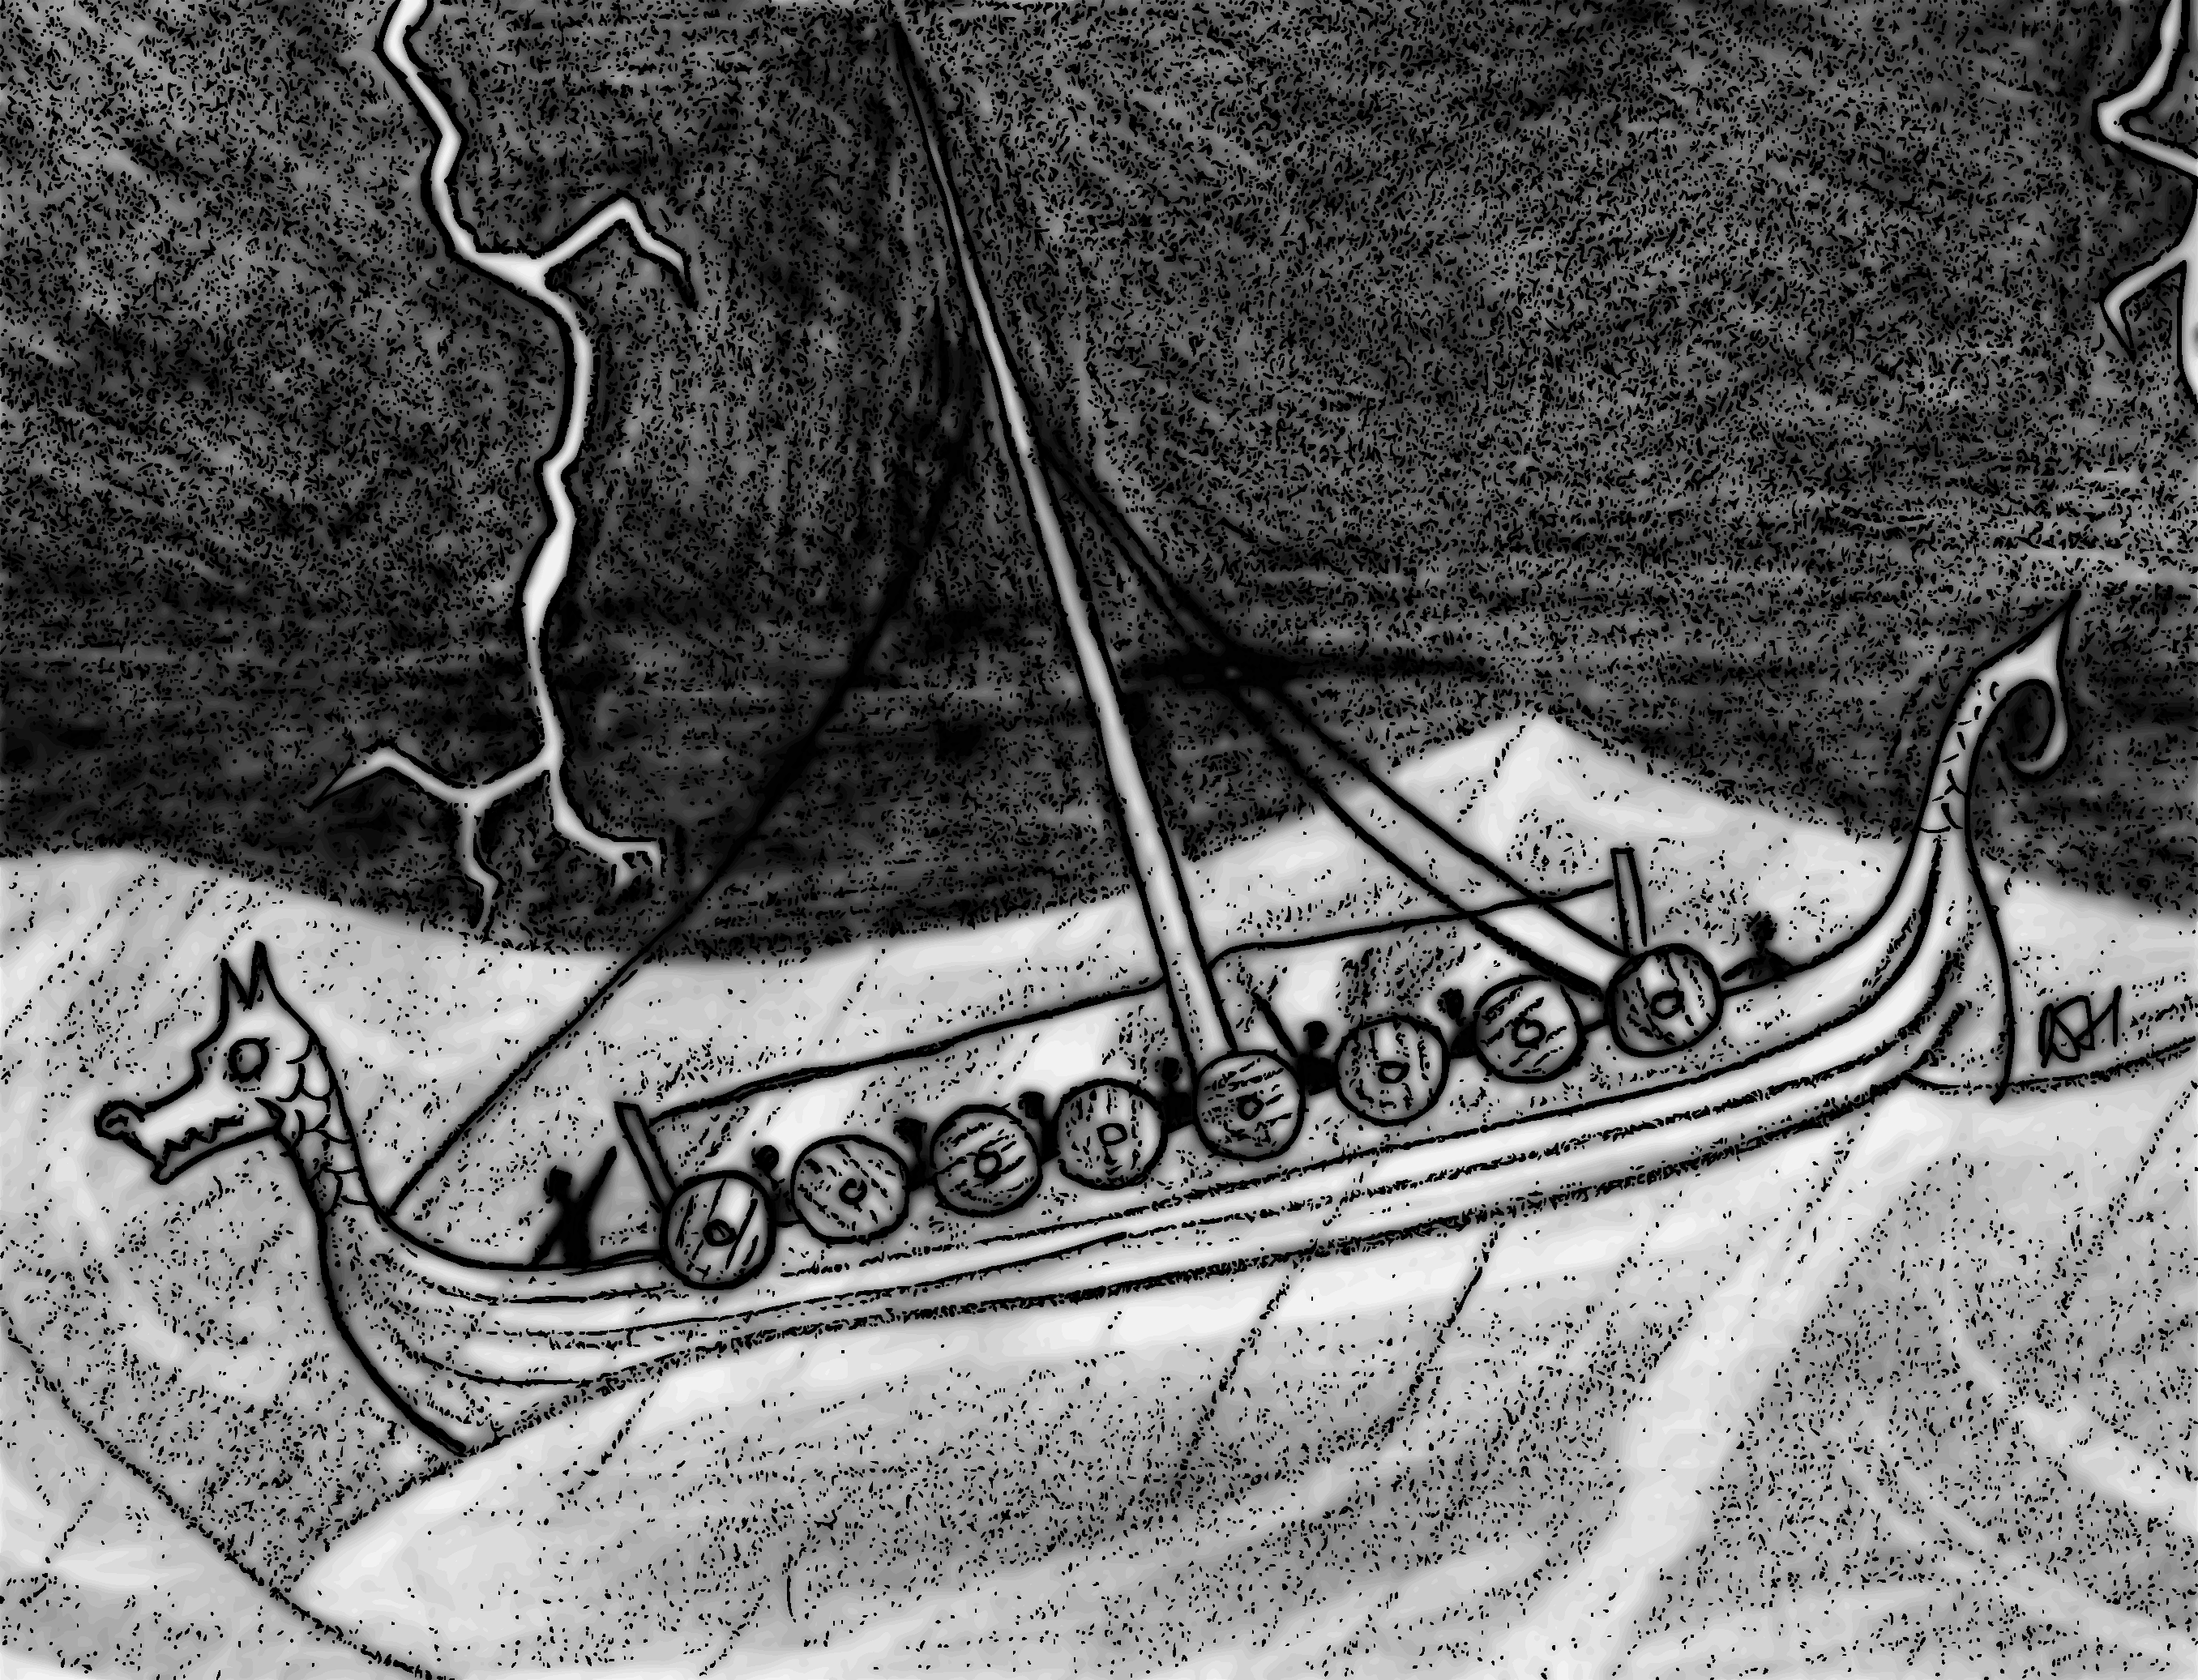
\includegraphics[width=\columnwidth]{vikingship.pdf}\label{vikingship}


\noindent
\begin{minipage}{\columnwidth}

\captionof{table}{Obstacles and Hindrances}\label{obstacles}
\noindent
\begin{tabular}{|p{.7\columnwidth}|p{.2\columnwidth}|}
\hline
Situation				& Modifier \\
\hline\hline
\rowcolor[gray]{.9}Chasm			& +3 \\
Cliff			& +3 \\
\rowcolor[gray]{.9}Dust/Sandstorm	& $\times$3 \\
Freezing		& +1 \\
\rowcolor[gray]{.9}Heavy wind		& +2 \\
Heavy fog		& +1 \\
\rowcolor[gray]{.9}Ice storm		& +2 \\
Mud				& $\times$2 \\
\rowcolor[gray]{.9}Rain, heavy		& $\times$2 \\
Rain, light		& +1 \\
\rowcolor[gray]{.9}Rain, torrential	& $\times$3 \\
Ravine			& +$^1$/$_2$ \\
\rowcolor[gray]{.9}Ridge			& +1 \\
River*			& +1 \\
\rowcolor[gray]{.9}Scorching		& +1 \\
Blizzard		& $\times$4 \\
\rowcolor[gray]{.9}Snow, normal	& $\times$2 \\
Stream			& +$^1$/$_2$ \\
\hline
\end{tabular}
\noindent\begin{tabular}{p{.95\columnwidth}}
*This modifier does not apply if a bridge is present. \\
\end{tabular}\vspace{.5em}

\end{minipage}

\section{WATER TRAVEL}

\index{Water Travel}There are two methods of traveling on water.  Each method assumes the proper craft, gear, and crew.

\subsection{RIVER}

The type of boat and the flow of the current determine movement value on a river.  When traveling downstream, the speed of the current is added to the speed of the boat.  When traveling upstream, the speed of the current is subtracted from the speed of the boat.  

Obstacles can be avoided when going upstream, but going downstream requires a good map or knowledgeable guide.  If placed in a harmful situation, the character piloting the craft must make a wisdom check to prevent capsizing.  Capsized boats are swept downstream and are destroyed by waterfalls or powerful rapids.

\subsection{OCEAN VOYAGE}

Ocean travel is primitive and dangerous.  Deep-sea sailing requires accurate instruments and an adequate crew.  Ships typically use sails but can be powered by oars.  Ships are rated based on their movement and seaworthiness.

\noindent
\begin{minipage}{\columnwidth}

\captionof{table}{Boat Movement}\label{boatmovement}
\noindent
\begin{tabular}{|p{.2\columnwidth}|p{.15\columnwidth}|p{.1\columnwidth}|p{.15\columnwidth}|p{.15\columnwidth}|}
\hline
Vessel	& Feet/ Round	& MPH	& Cargo	& Length \\
\hline\hline
\rowcolor[gray]{.9}Kayak			& 200	& 2		& 250 lbs.		& 8--10 ft. \\
Canoe, small	& 200	& 2		& 550 lbs.		& 10--15 ft. \\
\rowcolor[gray]{.9}Canoe, war		& 180	& 2		& 800 lbs.		& 25--35 ft. \\
Curragh			& 60	& 1*	& 600 lbs.		& 8--10 ft. \\
\rowcolor[gray]{.9}Keelboat, raft	& 60	& 1*	& 2,000 lbs.	& 15--20 ft. \\
Barge			& 60	& 1*	& 4,000 lbs.	& 25--40 ft. \\
\rowcolor[gray]{.9}Rowboat			& 160	& 1.5*	& 600 lbs.		& 8--12 ft. \\
\hline
\end{tabular}
\noindent\begin{tabular}{p{.95\columnwidth}}
*These vessels can triple their movement when the sail is raised and wind is favorable. \\
\end{tabular}\vspace{.5em}

\end{minipage}

A base mile per hour (MPH) is the distance a boat moves per hour.  If the number is separated by a slash, the first number is the sail speed and the second is the rowing speed.  Per round, a ship moves a number of yards equal to its MPH multiplied by 10.  Emergency move is the top speed a ship can move.  Emergency move strains the ship's resources severely and can only be sustained for a short amount of time before it starts to cause damage to the ship and her crew.  Seaworthiness is the chance a ship may sink during a dangerous situation like a storm, an extended voyage, being rammed, or an encounter with hidden obstacles.  If a d\% roll is higher than the seaworthiness rating, the ship sinks.  Anchored vessels have a +50\% bonus to their seaworthiness.

\noindent
\begin{minipage}{\columnwidth}

\captionof{table}{Ship Movement}\label{shipmovement}
\noindent
\begin{tabular}{|p{.25\columnwidth}|p{.1\columnwidth}|p{.2\columnwidth}|p{.25\columnwidth}|}
\hline
Ship	& MPH	& Emergency Move	& Seaworthiness \\
\hline\hline
\rowcolor[gray]{.9}Caravel		& 4		& 5		& 70\% \\
\rowcolor[gray]{.9}Coaster		& 3		& 4		& 50\% \\
Cog			& 3		& 4		& 65\% \\
\rowcolor[gray]{.9}Curragh		& 2/3	& 10	& 55\% \\
Drakkar		& 2/4	& 12	& 50\% \\
\rowcolor[gray]{.9}Dromond		& 2/9	& 12	& 40\% \\
Galleon		& 3		& 6		& 75\% \\
\rowcolor[gray]{.9}Great galley	& 3/6	& 11	& 45\% \\
Knarr		& 4/2	& 12	& 65\% \\
\rowcolor[gray]{.9}Longship	& 5/2	& 13	& 60\% \\
\hline
\end{tabular}

\end{minipage}

\subsection{WEATHER CONDITIONS}

\index{Weather}The weather can affect the movement value of ships.  Use the multipliers from the table to determine the final movement value of the ship. 

Weather is fairly consistent for the entire day.  The GM can decide the weather conditions for each day or roll for it randomly based on the current season.

Generally winds are favorable but sometimes can be adverse.  If winds are determined then roll 1d6; on a 5 or 6, the winds are adverse.  Adverse winds, storms and even worse weather blow a ship off course by half its movement modified by the wind ($\times$2 or more).

A strong wind applies a $-2$ penalty to all ranged attacks and affects movement.  Storms make it impossible to fire normal missiles and can knock creatures back.  Gale force winds make it impossible to fire any missile, including siege missiles, can uproot small trees, knock down weak structures, and endanger ships.  Hurricane force winds can destroy sturdier buildings and tear ships apart.

\noindent
\begin{minipage}{\columnwidth}

\captionof{table}{Weather Movement Modifiers for Ships}\label{weathershipmods}
\noindent
\begin{tabular}{|p{.27\columnwidth}|p{.3\columnwidth}|p{.28\columnwidth}|}
\hline
Weather			& Sailing Modifier	& Rowing Modifier \\
\hline\hline
\rowcolor[gray]{.9}Adverse			& $\times$$^1$/$_2$		& $\times$1 \\
Windless/Calm	& $\times$0*		& $\times$1 \\
\rowcolor[gray]{.9}Favorable wind	& 			&  \\
\rowcolor[gray]{.9}\hspace{2em}Average		& $\times$2		& $\times$1 \\
\hspace{2em}Strong		& $\times$3		& $\times$1** \\
\rowcolor[gray]{.9}Gale			& $\times$4**		& $\times$$^1$/$_2$** \\
Hurricane		& $\times$5***	& $\times$$^1$/$_2$*** \\
\rowcolor[gray]{.9}Light breeze	& $\times$1		& $\times$1 \\
Storm			& $\times$3**		& $\times$$^1$/$_2$** \\
\hline
\end{tabular}
\noindent\begin{tabular}{p{.95\columnwidth}}
*A ship cannot move using sails in calm winds or less. \\
**Seaworthiness check is required. \\
***Seaworthiness check at $-45$\% penalty is required. \\
\end{tabular}\vspace{.5em}

\end{minipage}

\noindent
\begin{minipage}{\columnwidth}

\captionof{table}{Random Wind}\label{randomwind}
\noindent
\begin{tabular}{|p{.05\columnwidth}|p{.25\columnwidth}|p{.25\columnwidth}|p{.25\columnwidth}|}
\hline
2d6	& Spring/Fall			& Summer			& Winter \\
\hline\hline
\rowcolor[gray]{.9}2	& Windless/calm		& Windless/calm		& Windless/calm \\
3	& Windless/calm		& Windless/calm		& Light breeze \\
\rowcolor[gray]{.9}4	& Light breeze		& Windless/calm		& Light breeze \\
5	& Moderate winds	& Light breeze		& Moderate winds \\
\rowcolor[gray]{.9}6	& Moderate winds	& Light breeze		& Strong winds \\
7	& Strong winds		& Moderate winds	& Strong winds \\
\rowcolor[gray]{.9}8	& Storm				& Moderate winds	& Storm \\
9	& Storm				& Strong winds		& Storm \\
\rowcolor[gray]{.9}10	& Gale				& Storm				& Gale \\
11	& Gale				& Gale				& Gale \\
\rowcolor[gray]{.9}12	& Hurricane*		& Hurricane*		& Hurricane* \\
\hline
\end{tabular}
\noindent\begin{tabular}{p{.95\textwidth}}
*Hurricanes occur only if the previous day's weather was gale.  Otherwise, treat hurricane as gale. \\
\end{tabular}\vspace{.5em}

\end{minipage}

\section{AERIAL MOVEMENT}

\index{Movement!Aerial}Aerial movement is handled under normal movement rules.  Weather modifies aerial movement and is essentially the sky's ``terrain."  Clear skies, with no more than moderate winds, are considered clear terrain for aerial movement.  The GM may choose the weather or determine it randomly.  To determine randomly, the GM rolls for wind conditions as above, using Table \ref{randomwind}.  If precipitation is not automatically indicated (such as storm, gale, etc.), the GM must roll 1d6.  In summer and winter, a roll of 6 on this die indicates rain or snow.  In spring and fall, a roll of 5 or 6 indicates rain.  Drier regions need not be checked, while wetter regions may have greater chance for precipitation.

Tiny flyers (the size of an eagle or smaller) are driven from the sky in a strong wind.  Man-sized flyers are buffeted out of the skies in gale force winds and large flyers cannot fly in storms.  Nothing can fly in a hurricane without magical protection.

The modifiers from this table are cumulative.  For example: gale force winds with rain applies a modifier of $^1$/$_2$~$\times$~$^1$/$_4$ = $^1$/$_8$, and strong winds with rain applies a modifier of $^1$/$_4$.

\noindent
\begin{minipage}{\columnwidth}

\captionof{table}{Aerial Movement Modifiers}\label{aerialmods}
\noindent
\begin{tabular}{|p{.45\columnwidth}|p{.45\columnwidth}|}
\hline
Condition		& Modifier \\
\hline\hline
\rowcolor[gray]{.9}Hurricane		& Impossible \\
Gale			& $\times$$^1$/$_4$ \\
\rowcolor[gray]{.9}Storm			& $\times$$^1$/$_4$ \\
Rain, snow		& $\times$$^1$/$_2$ \\
\rowcolor[gray]{.9}Strong wind		& $\times$$^1$/$_2$ \\
\hline
\end{tabular}

\end{minipage}

\subsection{Aerial Combat}

\index{Combat!Aerial}For the most part, aerial combat is treated the same as ground combat, with a few differences.  Most flyers (flying creatures, magical items and vehicles) cannot stop in place; they must keep moving forward to remain airborne, and since combat takes place in three dimensions, attacks can come from any direction, including above and below.  Aerial combat takes more game time.  Essentially, aerial combat consists of combatants maneuvering into position, taking dives and passes, and maneuvering back into a favorable position to attack again.  Rounds go by where combatants can do nothing except circle around, rolling initiative.  During these ``pass" rounds, combatants can escape, climb or dive as part of their movement.

The GM may treat flying movement values the same as ground movement. However, in purely aerial combat scenarios, precise distance measurements are not really necessary.   If using scale figurines, the GM may change the scale of the aerial battles and use the flying movement value as analogous to actual inches on a playing surface.  It is important to modify all combatants' movement values by any applicable weather or other modifiers before beginning the combat.

\paragraph{Altitude:} The GM must have a rough estimate of the number of feet of altitude at which the combatants are flying (see also Damage, Stalling, and Crashing).  It is assumed that most aerial combat is conducted at the same relative altitude; however, a flyer can attempt to change its altitude to gain a combat advantage.  For simplicity sake, while ascending (climbing) movement value is halved, and while descending (diving) movement value is doubled.  

A flyer above another can dive upon an opponent to gain a charge bonus to their attack.  During a successful dive attack, natural talons and claws as well as lances and spears cause double damage.  Flying creatures require natural weaponry and mounted flyers (including those using a fly spell, device or vehicle) require a large weapon to attack a flyer directly below them.  Because of the difficult angle, attacks made against a flyer directly above a flying combatant suffer a $-2$ penalty.

\index{Initiative!Flying}\paragraph{Initiative:} Flyers with better maneuver classes and better speed classes receive distinct advantages (see tables below).  At the beginning of combat, note the numerical values of the maneuver classes and speed classes of all combatants (ranging from 1 to 5).  The more agile combatant receives a bonus to his initiative rolls, between 0 and $-4$, equal to the difference between their maneuver class and the maneuver class of their opponent.  A 1-point bonus is also awarded to the faster opponent for every 2 points of difference between their speed classes, rounded up (maximum of $-2$ bonus when it's fast or god-like vs. slow).  Both bonuses may go to the same combatant for a total possible bonus of $-6$, or may be split between them.  Initiative is rolled (and modified) each round, whether any attacks occur during that round or not (Refer to Escaping, and see also Passes, Engagements and Dogfights).

\index{Speed Classes}\paragraph{Speed Class:} Flyers can be divided into 5 speed classes based upon their flying movement value.  A flyer can intentionally fly at a slower speed class, but unless this is expressly stated, speed class is always considered to be at the flyer's normal movement value.  Movement modifiers from diving or climbing do not affect the flyer's speed class.

\noindent
\begin{minipage}{\columnwidth}

\captionof{table}{Speed Classes}\label{speedclasses}
\noindent
\begin{tabular}{|p{.45\columnwidth}|p{.45\columnwidth}|}
\hline
Speed Class		& Movement Value \\
\hline\hline
\rowcolor[gray]{.9}1---Slow		& 12 or less \\
2---Average		& 13--24 \\
\rowcolor[gray]{.9}3---Quick		& 25--36 \\
4---Fast		& 37--48 \\
\rowcolor[gray]{.9}5---God-like*	& 49 or higher \\
\hline
\end{tabular}
\noindent\begin{tabular}{p{.95\textwidth}}
*God-like may include some hasted flyers. \\
\end{tabular}\vspace{.5em}

\end{minipage}

\index{Maneuver Classes}\paragraph{Maneuver Class:} Creatures, magical items and other vehicles that can fly will have a maneuver class listed alongside their movement value. Among other things, this value describes how tight of a turn the creature or object can make, ranging from 1---perfect (magical flight) to 5---clumsy (large, heavy fliers).   A flyer can intentionally fly with less agility, but unless this is expressly stated, maneuver class is always considered to be at the flyer's normal rating.

\noindent
\begin{minipage}{\columnwidth}

\captionof{table}{Maneuver Classes}\label{maneuverclasses}
\noindent
\begin{tabular}{|p{.18\columnwidth}|p{.08\columnwidth}|p{.22\columnwidth}|p{.08\columnwidth}|p{.19\columnwidth}|}
\hline
Maneuver Class 	& Turns	& Passes			& Hover & Momen\-tum \\
\hline\hline
\rowcolor[gray]{.9}1---Perfect		& 12	& Normal			& Yes 	& None \\
2---Good		& 6		& 1 per round		& Yes		& None \\
\rowcolor[gray]{.9}3---Average		& 3		& 1 per 2 rounds	& No		& $^1$/$_2$ Move \\
4---Poor		& 2		& 1 per 3 rounds	& No	& $^1$/$_2$ Move \\
\rowcolor[gray]{.9}5---Clumsy		& 1		& 1 per 6 rounds	& No		& $^1$/$_2$ Move \\
\hline
\end{tabular}

\end{minipage}

\paragraph{Hover:} Perfect and good flyers can hover.  Flyers that can hover don't have to maintain momentum each round.  This allows them to maintain their altitude, or climb and dive without moving forward.

\paragraph{Momentum:} Indicates the minimum distance a flyer must travel during a round.  With the exception of perfect and good flyers, all other creatures must maintain forward momentum or else they stall in the air and fall.  Momentum can be maintained in any direction and a flyer can turn if they wish.  For example, a flyer with average maneuver class and a movement value of 12 must fly at least 6 and can make up to 3 turns while doing so.

\paragraph{Turns:} Flyers are limited to the number of direction changes (or turns) they can make in a single round.  In general, a single turn is a 30-degree angle, and 12 turns equal 360 degrees (a full circle).

\paragraph{Passes, Engagements and Dogfights:} Aerial combat is concerned with two things: maneuver class and speed class.  Unlike ground combat, aerial combat is about positioning and maneuvering.  Attackers position themselves to catch up with and strike their opponents who are likewise trying to evade attacks and intercept them.  Fast, agile flyers always have an advantage over slow, clumsier flyers.  

Passes represent the number of rounds it takes for a flyer to perform one melee or non-magical ranged attack (such as a breath weapon) upon a relatively stationary opponent.  Stationary opponents include those on the ground, those using a \textit{levitate} spell (or hovering in place) and those flyers with the same speed class as the attacker.  Passes can also represent the nature of aerial combat where flyers must break off, reposition, and then prepare for another attack, but this abstraction can be ignored if miniatures and scale measurements are used.

In aerial combat, the combatants will engage each other as they do in ground combat and enter a dogfight.  In addition to the initiative bonuses given to faster and more maneuverable flyers, the number of rounds between attacks can be increased or decreased based on the relative speed class.  Add or subtract the difference between the opponents' speed classes to the number of rounds per attack.  Only perfect flyers are able to treat aerial combat the same as ground combat.  They can attack their normal number of times each round, unless their opponent is faster.   All other maneuver classes are limited to 1 attack per round, regardless of bonuses.
 
In the following examples, MC is Maneuver Class and SC is Speed Class.
 
\paragraph{Example 1:} A flyer with an MC5/SC3 (clumsy but quick) versus a flyer with an MC3/SC1 (average and slow).  If the speed classes had been equal, the flyer with MC5 would attack once every six rounds, and the flyer with MC3 would attack once every two rounds, but there is a 2-point difference in speed class.  So, the flyer with MC5 would attack once per four rounds (6~$-$~2 = 4), and the flyer with MC3 would also attack once every four rounds (2~+~2 = 4).  The speed difference put them on even footing.
 
\paragraph{Example 2:} MC5/SC1 (clumsy and slow) vs. MC3/SC3 (average and quick).  MC5 would attack 1/8 rounds and the MC3 would attack once every round (the maximum).

\paragraph{Example 3:} MC5/SC1 (clumsy and slow) vs. MC2/SC5 (good and godlike).  There is now a 4-point difference, so MC5 would attack 1/10 rounds and MC2 still attacks only once per round.

\paragraph{Example 4:} MC5/SC5 (clumsy but godlike) vs. MC2/SC1 (good but slow).  MC5 attacks 1/2 rounds, due to its god-like speed, while MC2 is reduced to only 1/5 rounds.
 
\paragraph{Example 5:} MC5/SC1 (clumsy and slow) vs. MC1/SC4 (perfect and fast). MC5 attacks 1/9 rounds and MC1 gets its normal attacks each round (no change).
 
\paragraph{Example 6:} MC5/SC4 (clumsy but fast) vs. MC1/SC1 (perfect but slow).  MC5 attacks 1/3 rounds and MC1 is reduced to 1 normal attack every 4 rounds.

\paragraph{Escaping:} A flyer that is both faster and more maneuverable than its opponent can break off and escape during its initiative, with no free attack against it.  A flyer that is faster but equally or less maneuverable can escape during their initiative, but suffers the free attack against it.  A flyer that is slower but more maneuverable, must win the initiative roll to escape without a free attack against it, but can escape during a lost initiative by accepting a free attack against it.   A flyer that is slower and equally or less maneuverable than its opponent must win the initiative roll to escape, but still suffers the free attack against it.  Ground based opponents may attempt to escape normally.

\paragraph{Breath Weapons \& Spells:} It's easier to employ a breath weapon or cast a spell with an effective area on the ground than it is in the air.  When using a breath weapon, a 60-degree arc in front of the creature is the blast area.  When a spell with an effective area is cast, the blast area is half the size of the effective area starting from the center.  Creatures inside the blast area roll normal saving throws.  Any creatures caught inside the effective area, but outside the blast area, receive a +2 bonus to applicable saves.

\paragraph{Missile Fire:} Mounted flyers that are in motion (including those using a \textit{fly} spell, a device or vehicle), suffer the same penalty while firing a ranged weapon as if they were mounted on the ground.  A hovering creature, even if mounted or using a \textit{fly} spell, doesn't suffer this penalty.
 
\paragraph{Damage, Stalling, and Crashing:} With the exception of perfect flyers, those that sustain damage equal to or greater than 50\% of their maximum hit points are reduced to half movement value and must immediately land.  These flyers can usually glide safely to the ground but cannot climb until healed to above 50\%.  Good flyers also lose their ability to hover until healed to above 50\%.  If the GM determines that no safe landing spot is available, the result is a crash landing.  The GM must adjudicate crash landings based on factors, such as the altitude and ground terrain, as well as the speed, size and type of flyer, but the damage should be no less than 2d6 and no more than 10d6. 

In general, the faster a flyer is moving when it crashes, the more damage it takes.  If a flyer strikes a solid object in mid-air, it crashes, suffering damage equal to 2d6 per its current speed class (10d6 maximum).  A flyer that has crashed into an obstacle immediately stalls and falls.  Flyers that stall in mid-air (see also Momentum), or those whose fly spell suddenly ends, fall straight down a number of feet equal to five times their momentum requirement.  A flyer that hits the ground before the end of the fall crashes; taking 1d6 damage per current speed class (1--5) for every 10 feet of fall completed.  The minimum damage is 2d6 and the maximum damage is 20d6.  A stalled flyer that doesn't crash by the end of its fall, assuming it is still conscious and less than 50\% damaged, can regain its composure and begin to fly normally again.  The faster the flyer is moving when it stalls the farther it falls. For this reason, fast flyers (movement value of 48) prefer combat at altitudes in excess of 120 feet (48~$\div$~2 = 24~$\times$~5 = 120').  Slower flyers (movement value of 12) often attempt to conduct combat at lower altitudes of 30 feet (12~$\div$~2 = 6~$\times$~5 = 30') or around tree top level, to discourage a faster opponent from taking full advantage of its speed.

\section{BECOMING LOST}

\index{Becoming Lost}It's possible to become lost while traveling.  Characters are either lost or hopelessly lost.

\subsection{LOST}

Becoming lost occurs when the travelers don't know the route to their destination but know how to return to the starting point.  Finding the right direction or returning to the starting point is simply a matter of time.  This generally occurs when following unfamiliar paths or poorly marked trails, or when consulting poorly drawn maps or badly worded directions.  Becoming lost is a setback but is rarely dangerous.

\subsection{HOPELESSLY LOST}

Becoming hopelessly lost happens when characters don't know where they are, which way to go, or how to get back where they started.  A check should be made whenever the characters move overland without following a road, river, or well-traveled trail, and whenever a river they are following empties into a swamp, estuary, or delta.  One check should be made each day these conditions persist.  If the die roll is less than the modified percentage, the characters are hopelessly lost.

If a party is hopelessly lost, they make no further checks until they find a way to regain their bearings (they get directions, find a road, etc.).  The GM should refrain from telling players that their characters are lost.  The GM should randomly determine the general direction the party travels per day while they're lost by rolling 1d8; 1 is north, 2 is north-east, 3 is east, 4 is south-east, 5 is south, 6 is south-west, 7 is west, 8 is north-west.

\noindent
\begin{minipage}{\columnwidth}

\captionof{table}{Chance of Becoming Hopelessly Lost}\label{lostchance}
\noindent
\begin{tabular}{|p{.7\columnwidth}|p{.2\columnwidth}|}
\hline
Surroundings			& \% Chance \\
\hline\hline
\rowcolor[gray]{.9}Level, open ground		& 10\% \\
Rolling ground			& 20\% \\
\rowcolor[gray]{.9}Lightly wooded			& 30\% \\
Rough, wooded and hilly	& 40\% \\
\rowcolor[gray]{.9}Swamp					& 60\% \\
Mountainous				& 50\% \\
\rowcolor[gray]{.9}Open sea				& 20\% \\
Thick forest			& 70\% \\
\rowcolor[gray]{.9}Jungle					& 80\% \\
\hline
\end{tabular}

\end{minipage}

\noindent
\begin{minipage}{\columnwidth}

\captionof{table}{Lost Modifiers}\label{lostmods}
\noindent
\begin{tabular}{|p{.7\columnwidth}|p{.2\columnwidth}|}
\hline
Condition				& Modifier \\
\hline\hline
\rowcolor[gray]{.9}No landmarks*			& +50\% \\
Darkness				& +70\% \\
\rowcolor[gray]{.9}Overcast				& +30\% \\
Navigator with group	& $-30$\% \\
\rowcolor[gray]{.9}Landmark sighted		& $-15$\% \\
Local guide				& Variable** \\
\rowcolor[gray]{.9}Poor trail				& $-10$\% \\
Raining					& +10\% \\
\rowcolor[gray]{.9}Directions, map, tools	& Variable** \\
Fog or mist				& +30\% \\
\hline
\end{tabular}
\noindent\begin{tabular}{p{.95\columnwidth}}
*Includes sailing out to sea beyond sight of land. \\
**GM decides usefulness of guide or directions. Generally, more expensive guides or maps are more useful. \\
\end{tabular}\vspace{.5em}

\end{minipage}

\section{SWIMMING}

\index{Swimming}Swimming is a skill that a character can learn.  Characters are capable of swimming a number of yards in a single round equal to half their movement value multiplied by 10.  Swimmers can gain a burst of speed, thus moving their full movement value in a single round, by rolling a strength check against half their strength score (exceptional strength counts as 9).  \index{Armor!Effects on Swimming}Characters wearing metal armor instantly sink to the bottom; however, they can walk along the bottom at $^1$/$_3$ their movement value.  

\index{Constitution!and Swimming}A character can normally swim (at half speed) for a number of hours equal to his constitution score.  A constitution check (or a save vs. death if no constitution score is known) must be made for each additional hour of swimming.  If a swimmer fails this constitution check, he must tread water for half an hour before he can continue swimming (this time counts as time spent swimming).  Furthermore, additional hours spent swimming reduces constitution by 1 point temporarily and applies a cumulative penalty of $-1$ to all attack rolls.  A character drowns if his constitution score drops to 0 while swimming.  

Normal travel assumes swimming in calm waters.  Choppy water or swimming against the tide requires a constitution check every hour of swimming.  Rough water or swimming against a heavy tide requires a constitution check every half hour.  Stormy water requires a constitution check every round.  The GM may modify the constitution points lost in rougher waters.

Characters can swim fast for longer distances but at an increased risk.  A swimmer can move at his full movement value but he must make a constitution check every hour, his strength and constitution are reduced by 1 point every hour, and a cumulative $-2$ penalty to his attack rolls is applied every hour.  Characters can swim twice their movement value but must roll a constitution check every turn, and the penalties are accrued every turn spent swimming.  Drowning occurs when either strength or constitution reaches 0.

Characters can recover lost ability score points and attack penalties by resting.  Each day of rest recovers 1d6 ability points (1d3 points for strength and constitution if swimming at a hustle) and restores 2d6 points worth of attack penalties.  

\subsection{HOLDING A CHARACTER'S BREATH}

\index{Holding One's Breath}If able to get a gulp of air in advance, characters can hold their breath for a number of rounds equal to $^1$/$_3$ their constitution score (round up).  If characters exert themselves (moving more than half their movement value, fighting, or swimming in rough water), this time is halved (rounded up).  Characters in metal armor are considered to be exerting themselves.  If unable to get a gulp of air, these times are reduced by half.  All characters are capable of holding their breath for at least one round regardless of circumstances.  Holding one's breath beyond this time requires a constitution check each round.  Each subsequent check suffers a -2 cumulative penalty.  On a failed check, the character must breathe.  If he cannot breathe then he drowns.

\index{Swimming!Diving}\index{Diving}\paragraph{Diving:} Regardless of movement, swimmers can swim downwards 20 feet in a single round.  A brief run or jumping several feet above the water adds 10 feet of depth to the initial dive.   For every 10 feet of height above the water an additional 5 feet of depth can be added up to a maximum of 20 additional feet.  By contrast, if prepared for shallow water, a character can dive from a height of up to 50 feet without being injured, as long as the water is at least 3-feet deep per 10 feet of the height of the dive.  

\paragraph{Surfacing:} Regardless of movement, swimmers can rise at the rate of 20 feet per round.  Characters floating to the surface (such as dead or unconscious characters) rise at a rate of 5 feet per round.
 
\subsection{VISION UNDERWATER}

\index{Vision!Underwater}Under normal conditions (bright sunlight), vision extends out to 50' in freshwater and 100' in saltwater.  For every 10' below the surface, vision is reduced by 10' until it becomes pitch black.  On overcast days, normal vision underwater is reduced to half, and characters cannot see at all on moonless nights.  Artificial light sources, such as magic, only illuminate half their normal area underwater.

\section{CLIMBING}

\index{Climbing}Climbing is a general skill anyone can learn.  For most characters, climbing requires specialized equipment such as ropes and pitons.  Only thieves can climb without the use of equipment.  A climb check is made whenever a character attempts to ascend more than 10 feet.  The base climb check is 40\% modified by special conditions.  Thieves use their climb walls rate to climb.  The climb check is made before the character begins climbing.  If the check is successful, the character need not make a new check unless conditions worsen.  If the character fails their initial climb check they find no means of climbing and cannot even begin.  A character may retry a failed climb check only if conditions would improve their check or they find a suitable location at least half-a-mile away.

\noindent
\begin{minipage}{\columnwidth}

\captionof{table}{Climbing Modifiers}\label{climbingmods}
\noindent
\begin{tabular}{|p{.7\columnwidth}|p{.2\columnwidth}|}
\hline
Situation								& Modifier \\
\hline\hline
\rowcolor[gray]{.9}Prominent handholds (branches, ledges)	& +40\% \\
Rope and wall							& +55\% \\
\rowcolor[gray]{.9}Sloped inward							& +25\% \\
Armor									& \\
\hspace{2em}Banded, splint						& -25\% \\
\rowcolor[gray]{.9}\hspace{2em}Plate									& -50\% \\
\hspace{2em}Scale, chain							& -15\% \\
\rowcolor[gray]{.9}\hspace{2em}Studded leather, padded				& -5\% \\
Character race*							& \\
\hspace{2em}Dwarf									& -10\% \\
\rowcolor[gray]{.9}\hspace{2em}Gnome									& -15\% \\
\hspace{2em}Halfling								& -15\% \\
\rowcolor[gray]{.9}Encumbrance**							& -5\% \\
Surface condition						& \\
\hspace{2em}Slightly slippery (wet/ crumbling)	& -25\% \\
\rowcolor[gray]{.9}\hspace{2em}Slippery (icy/ slimy)					& -40\% \\
Climber $^1$/$_2$ HP or less			& -10\% \\
\hline
\end{tabular}
\noindent\begin{tabular}{p{.95\columnwidth}}
*Same modifiers listed for thieves. Do not apply twice. \\
**This penalty is cumulative for each point a character's speed is reduced below their base. \\
\end{tabular}\vspace{.5em}

\end{minipage}

\subsection{CLIMB SPEED}

\index{Climbing Speed}Climb speed is determined by the surface a character is climbing on.  All characters are able to climb their movement value in feet, multiplied based on the type of surface, in one direction (up, down, sideways, or diagonal) per round.  Thieves climb at double the speed of a normal character and their speed modifiers are listed in brackets [\#].

Climbing characters cannot use items requiring two hands, unless they find secure footing.  If struck while climbing, regardless of damage, a climb check must be made immediately to maintain hold.  If a roped character fails, he must spend a round to regain his handhold.  An un-roped character falls on a failure.

\noindent
\begin{minipage}{\columnwidth}

\captionof{table}{Climbing Speed Modifiers}\label{climbinbspeedmods}
\noindent
\begin{tabular}{|p{.35\columnwidth}|p{.15\columnwidth}|p{.15\columnwidth}|p{.15\columnwidth}|}
\hline
Surface				& Dry					& Slightly Slippery		& Slippery \\
\hline\hline
\rowcolor[gray]{.9}Very smooth*		& $^1$/$_4$ [$^1$/$_2$]	& -- [$^1$/$_4$]		& --** \\
Smooth, cracked*	& $^1$/$_2$ [1]			& $^1$/$_3$ [$^2$/$_3$] & $^1$/$_4$ [$^1$/$_2$] \\
\rowcolor[gray]{.9}Rough*				& 1 [2]					& $^1$/$_3$ [$^2$/$_3$]	& $^1$/$_4$ [$^1$/$_2$] \\
Rough w/ledges		& 1 [2]					& $^1$/$_2$ [1]			& $^1$/$_3$ [$^2$/$_3$] \\
\rowcolor[gray]{.9}Ice wall			& --					& --					& $^1$/$_4$ [$^1$/$_2$] \\
Tree				& 4 [8]					& 3 [6]					& 2 [4] \\
\rowcolor[gray]{.9}Sloping wall		& 3 [6]					& 2 [4]					& 1 [2] \\
Rope and wall		& 2 [4]					& 1 [2]					& $^1$/$_2$ [1] \\
\hline
\end{tabular}
\noindent\begin{tabular}{p{.95\columnwidth}}
*Non-thieves require climbing gear to climb these surfaces. \\
**It is impossible to climb very smooth, slippery surfaces with mundane tools. \\
\end{tabular}\vspace{.5em}

\end{minipage}

\subsection{CLIMBING TOOLS}
\index{Climbing!Climbing Tools}The basic tools for climbing are pitons (spikes), ropes, and ice axes.  Tools do not actually aid in climbing; rather, they prevent falling.  A character can only fall as far as their rope or twice the distance to the last piton they placed.  Pitons have a 15\% chance of coming loose in the case of a fall.  Characters still take normal falling damage (1d6 per 10 feet) representing the jerking action of the rope catching their fall.

Characters roped together can prevent each other from falling, but may pull down their allies.  When a character falls, the characters directly roped to him must make a climb check.  A $-10$\% penalty is applied for each falling character after the first.  Success indicates the fall is prevented and no damage is taken.  Failure indicates that character also falls and the process is repeated until someone succeeds or everyone falls.

\subsection{RAPPEL}
Characters can rappel down the side of a surface provided a strand of rope is firmly attached to the top.  Characters can safely rappel a number of feet per round equal to their movement value times ten.  A climb check is made each round with a +50\% bonus if someone is holding the rope at the bottom.  Free rappelling (rappelling without someone at the bottom) provides a +30\% bonus to the climb check.

\section{VISION AND LIGHT}

\index{Vision}Assuming an Earth-sized world, the horizon is viewable from about 12 miles away, and it's possible to see tall mountains at least 60 miles away.  In optimum conditions (clear day with no obstructions), it's possible to see a moving, man-sized object at a distance of 1,500 yards.  Details cannot be made out at this distance, and an immobile creature cannot be seen.

At 1,000 yards, a man-sized object, whether stationary or mobile, can be spotted.  Size and shape can be determined but no other details, unless they're unique.  At 500 yards, a man-sized object has a discernable size, shape, and color, and the creature's type is distinguishable.  Specific details cannot be made out unless large and bold or distinct.

At 100 yards, general details can be made out such as a heraldic symbol or coat of arms.  Most actions (such as who is attacking whom) can be ascertained.  At 10 yards, all details but the minutest are clear.  There are several conditions that can alter the normal distance at which objects can be spotted.

``Movement" indicates the distance at which a moving object can be seen.  ``Spotted" is the maximum distance a mobile or immobile object can be seen.  ``Type" indicates the maximum range at which general details can be discerned; race, weapons, clothing, etc.  ``Ident." is the range at which reasonably exact details can be identified.  ``Detail" range means most actions can be seen clearly.

Size can affect the distance as well.  When looking at a small creature, all categories are reduced by one step per size category except the ``detail" range.  When looking at large creatures, the ``movement," ``spotting," and ``type" ranges are doubled for each size category above medium.

\noindent
\begin{minipage}{\columnwidth}

\captionof{table}{Visibility Ranges (In Yards)}\label{visranges}
\noindent
\begin{tabular}{|p{.2\columnwidth}|p{.1\columnwidth}|p{.1\columnwidth}|p{.1\columnwidth}|p{.1\columnwidth}|p{.1\columnwidth}|}
\hline
Condition				& Move\-ment	& Spot\-ted	& Type		& Ident.	& Detail \\
\hline\hline
\rowcolor[gray]{.9}Clear sky				& 1,500		& 1,000		& 500		& 100		& 10 \\
Dense fog or blizzard	& 10		& 10		& 5			& 5			& 3 \\
\rowcolor[gray]{.9}Light fog or snow		& 500		& 200		& 100		& 30		& 10 \\
Mist, light rain		& 1,000		& 500		& 250		& 30		& 10 \\
\rowcolor[gray]{.9}Night, full moon		& 100		& 50		& 30		& 10		& 5 \\
Night, no moon			& 50		& 20		& 10		& 5			& 3 \\
\rowcolor[gray]{.9}Twilight				& 500		& 300		& 150		& 30		& 10 \\
\hline
\end{tabular}

\end{minipage}

\subsection{LIGHT}

\index{Light}In a completely lightless situation, normal vision is impossible.  Light sources vary in their effective area.  Most light sources require fuel and the time per fuel unit is listed.  Lanterns require oil, fires require wood or other fuel, candles rely on a tallow or wax and wick, torches have a one-time use unless wrapped with an oil soaked rag, and magic has a duration.

\noindent
\begin{minipage}{\columnwidth}

\captionof{table}{Light Sources}\label{lightsources}
\noindent
\begin{tabular}{|p{.35\columnwidth}|p{.15\columnwidth}|p{.35\columnwidth}|}
\hline
Source			& Radius	& Time per Fuel Unit \\
\hline\hline
\rowcolor[gray]{.9}Bonfire			& 50 ft.	& $^1$/$_2$ hour/armload \\
Campfire		& 35 ft.	& 1 hour/armload \\
\rowcolor[gray]{.9}Candle, tallow	& 5 ft.		& 10 minutes/inch \\
Candle, wax		& 6 ft.		& 20 minutes/inch \\
\rowcolor[gray]{.9}\textit{Continual light}	& 60 ft.	& Indefinite \\
Lantern			& 			& \\
\hspace{2em}Beacon		& 240 ft.*	& 2 hours/pint \\
\rowcolor[gray]{.9}\hspace{2em}Bull's-eye	& 60 ft.*	& 6 hours/pint \\
\hspace{2em}Hooded		& 30 ft.	& 6 hours/pint \\
\rowcolor[gray]{.9}\textit{Light}			& 20 ft.	& Variable \\
Torch			& 15 ft.	& 30 minutes \\
\hline
\end{tabular}
\noindent\begin{tabular}{p{.95\columnwidth}}
*Casts light in a cone-shaped beam.  A beacon lantern's far end is 90 feet wide and a bull's-eye lantern's far end is 20 feet wide. \\
\end{tabular}\vspace{.5em}

\end{minipage}

\subsection{INFRAVISION}

\index{Infravision}Some creatures have the special ability to see in the dark.  Infravision allows creatures to see in darkness as they would in normal light.  All details are recognizable, however, images are in black and white and therefore colors are not discernable.  Unless otherwise noted, infravision extends to 60 feet.

\subsection{DARKNESS}

\index{Darkness}Darkness is a condition applied when characters cannot see, either because they have limited visibility or because they've been blinded.  Characters can safely move in the darkness at $^1$/$_3$ their normal movement.  \index{Armor Class!Effects of Darkness}\index{Attack Roll!Effects of Darkness}Characters without adequate light also suffer a $-4$ penalty to attack rolls and saving throws and their armor class is 4 points worse (maximum 10).  

\subsection{USING A MIRROR}

\index{Mirrors}Characters can act using the guidance of a mirror or reflective surface.  Using a reflective surface to aid one's actions requires a light source.  All actions requiring an ability check, a proficiency check, or an attack roll suffer a $-2$ penalty.  Characters using a mirror to fight an opponent lose their dexterity bonus to armor class against that opponent.
 
\section{HEARING}

\index{Hearing}It's assumed that all characters can make out clear noises.  When hearing is difficult or when trying to pinpoint exact sounds (a single voice among multiple people), a hearing check is necessary.  Each race has a chance to hear equal to a 1st level thief.  A hearing check can either be a percentage roll or a 1d20 with the result needing to be equal or lower than the number in parentheses to successfully hear.

Hearing distinct sounds requires optimum conditions: helmet removed, standing still, and at least one round.  On a failed check, the character cannot discern the sound he was listening for until conditions improve.  On a successful check, he can hear the sound, although he may not necessarily know the source.  Further checks can be made to determine exact details like direction, the number of objects making the sound, how many people are speaking, etc.

\noindent
\begin{minipage}{\columnwidth}

\captionof{table}{Chance to Hear by Race}\label{hearingbyrace}
\noindent
\begin{tabular}{|p{.45\columnwidth}|p{.45\columnwidth}|}
\hline
Race		& 1d100 (1d20) \\
\hline\hline
\rowcolor[gray]{.9}Dwarf		& 15\% (3) \\
Elf			& 20\% (4) \\
\rowcolor[gray]{.9}Gnome		& 25\% (5) \\
Half-elf	& 15\% (3) \\
\rowcolor[gray]{.9}Halfling	& 20\% (4) \\
Human		& 15\% (3) \\
\hline
\end{tabular}

\end{minipage}

\section{DOORS}

\index{Doors}No check is necessary to open average doors.  Stuck, damaged, or incredibly heavy doors must be bashed or rammed to open properly.  Each character has a chance to bash doors based on their strength score.  There is no limit to the amount of times a character can attempt to force open a door, but each attempt reduces his chance by 1.  Two characters (or if using a suitable ram, three or more characters) can add half their force doors rating (rounded up) together to determine the overall check.  If they have enough room to run at the door, their full force doors ratings are added together.

A forced open door is destroyed or knocked off its hinges, making it impossible to properly close until repaired.  Forcing doors is also noisy, alerting anyone in the immediate vicinity.  The GM should make an immediate wandering monster check if a door is forced within a dungeon.

 
\subsection{SECRET AND CONCEALED DOORS}

\index{Secret Doors}\index{Concealed Doors}\index{Doors!Secret and Concealed}Secret doors are disguised as normal objects or walls, while concealed doors are simply hidden from plain sight.  For the average character, it takes 10 minutes (10 rounds or 1 turn) to search a 20' section of a wall.  If a secret or concealed door is found, the player also usually finds a means of opening it.  In cases of secret doors with no clear opening mechanism, one must be found.  Characters that can detect secret doors receive a +1 bonus to their check to find the opening mechanism, if they know the door exists.  Secret doors can be forced open at half the normal force doors rating.  

\section{INVISIBILITY}

\index{Invisibility}An invisible creature is invisible to everyone, including himself.  This imposes a $-3$ (or 15\%) penalty to complex actions, such as picking locks.  It is possible for moving creatures to collide with invisible creatures. The GM should remove invisible character's miniatures from the map and keep track of the invisible character's position.

Invisible creatures are undetectable by normal sight or infravision.  \textit{Detect magic} signals a magical presence in the area but does not pinpoint the creature's location.  They're also undetectable in smoke or fog, and while submerged in liquids; however, some objects, like flour, can stick revealing an invisible creature.  Invisibility doesn't mask sound or scent; therefore they can be pinpointed by noise or smell.  Light isn't hidden by invisibility, either.

If an invisible creature gives away their position, alert characters can make a save vs. spell to determine there's an invisible presence in the area.  Such disturbances include a peculiar smell, noise, or an invisible creature physically touching someone.  If the save is made, the character can, if he chooses, attack the general location at a $-4$ penalty.  If the save fails, the character doesn't know there's an invisible character until a new situation arises that allows another check.  An obvious disturbance, such as leaving muddy tracks, practically pinpoints the invisible creature's location, although the penalty to attack is the same.

\end{multicols}

\noindent\includegraphics[width=\textwidth]{araucariaportal.pdf}\label{araucariaportal}

\begin{multicols}{2}
 
\section{PLANES OF EXISTENCE}

\index{Planes of Existence}The multi-verse is made of many planes connected together, each governed by their own rules.  Planes are sphere-shaped worlds, infinite in size.  Time in the planes is based on perception, so that while one plane's time may flow faster in relation to another, five minutes while visiting a plane is always equal to five minutes to the visitor.

The Prime Material Planes contain the most earth-like worlds where the laws of gravity, the passage of time, and space function normally.  Surrounding each Prime is the Ethereal Plane, a misty, intangible world of proto-matter where tangible, finite demi-planes float about.  The GM's game world is located within one of these Primes.

Surrounding the Prime and Ethereal planes are the Inner planes made up of the energy, elemental, para-elemental, and quasi-elemental planes.  The elemental planes form the basic building blocks of matter: Water, Earth, Fire, and Air.  When the elemental planes touch, they form the para-elemental planes: Smoke, Ice, Ooze, and Magma.  The energy planes are made up of Positive Energy (the source of life) and Negative Energy (the source of death) planes.  When the elemental planes touch the Positive Energy plane they form the quasi-elemental planes of Lightning, Steam, Minerals, and Radiance.  When the elemental planes touch the Negative Energy plane they form the quasi-elemental planes of Salt, Vacuum, Ash, and Dust.  

Surrounding the inner planes is the Astral Plane, which also connects the Primes to each other and to the outer planes.  The Astral plane is an empty, weightless void of silver, with rare bits of solid matter and swirling color pools that serve as one-way gateways to the outer planes.  The colors are randomized but simply peering through the portals will reveal the landscape on the other side.  Astral creatures can propel themselves via thought; their base movement equal to 3$\times$ intelligence.  

Enveloping all the planes are the outer planes, also called the Planes of Power.  Each outer plane has its own unique rules on the effects of gravity, magic, and terrain.  Deities and other powerful beings call these planes home, and they're strongly aligned to the creatures that inhabit them.  The Outer Planes serve as the final resting spot of spirits and souls where they assimilate into the plane itself.

\section{DIMENSIONAL SPACE}

\index{Dimensional Space}Dimensional space is layered and complex.  The relationship between dimensional spaces, the planes of existence and other dimensional spaces is not fully understood.  It is generally believed, however, that the various planes of existence share infinite layers of dimensional space.  Most knowledgeable sages divide dimensional space into four major layers.  These are called Prime Dimensional, Extra-Dimensional, Non-Dimensional and Temporal Dimensional Spaces.  In addition to the four major layers of dimensional space, most sages believe that space can be accessed between these layers (Intra-dimensional Space) and created within these layers (Inter-dimensional Space).

\index{Dimensional Space!Prime}Prime Dimensional Space is the center of the cosmos.  The Prime Dimension contains all of the Alternate Prime Material Planes that co-exist with the GM's campaign world.  Alternate Prime Dimensions may exist that contain Alternate Prime Material Planes that do not co-exist with the GM's campaign world.  A \textit{teleport} spell accesses Prime Dimensional Space when cast on the Prime Material Plane.  Demi-planes are rare and generally temporary within Prime Dimensional Space.

\index{Extra-dimensional Space}Extra-dimensional Space exists outside, beyond or exceeding the limits of the Prime Dimension.  Extra-dimensional Space contains all of the planes that exist beyond the borders of the Prime Material Plane, including all inner and outer planes (ethereal, astral, Demiplane of Shadow, etc.).  Alternate Prime Dimensions may or may not have a corresponding Extra-dimensional Space.  Spells such as \textit{dimension door}, \textit{duo-dimension} and \textit{gate} access Extra-dimensional Space.  Demi-planes become more common and generally have longer durations within Extra-dimensional Space.  Creatures that originate from Extra-dimensional Space are commonly known as extra-planar creatures.  The energy to power spells and other magical effects is thought to originate from extra-dimensional sources.

\index{Non-dimensional Space}Non-dimensional Space exists outside, beyond and exceeding the limits of Extra-dimensional Space.  Non-dimensional Space exists outside the known multi-verse of the planes of existence.  If Alternate Prime Dimensions exist, Non-dimensional Space exists between them.  Permanent pocket dimensions within Non-dimensional Space, like those accessed by a \textit{bag of holding} or a \textit{portable hole} are also known as non-planar spaces.  A non-planar space can only be accessed through its specific portal.  Otherwise, only demi-planes exist in Non-dimensional Space, however, demi-planes within Non-dimensional Space are most often permanent constructs, and powerful deities have the ability, either individually or by working as a pantheon, to create Alternate Prime Dimensions from Non-dimensional Space. 

\index{Temporal Dimensional Space}Temporal Dimensional Space underpins and permeates all other dimensional spaces where time passes, but the GM may determine that time passes at different rates on different planes of existence or demi-planes, depending upon how the plane interacts with the Temporal Dimension.  It is known that certain regions of Non-dimensional Space are timeless, indicating that the Temporal Dimension does not completely overlap Non-dimensional Space.  Alternate Prime Dimensions may have separate Temporal Dimensions.  The GM may also determine that temporal planes and/or demi-plane(s) exist within Temporal Dimensional Space.

\index{Intra-dimensional Space}Intra-dimensional Space does not exist as its own separate space.  It occupies parts of two neighboring spaces.  Accessing Intra-Dimensional Space is commonly known as being out-of-phase.  An out-of-phase creature exists on both the Prime Material and Ethereal Plane, partially occupying Prime Dimensional and Extra-dimensional Space simultaneously.  The GM may determine that similar Intra-dimensional Space can be accessed between Extra-dimensional and Non-Dimensional Space, and between the Temporal Dimension and other dimensional spaces.  Some incorporeal creatures and objects are simply out-of-phase while others are made of pure magical or extra-dimensional energy.
 
\index{Inter-dimensional Space}Inter-dimensional Space exists within, amongst, and surrounded by adjacent dimensional space.  An inter-dimensional pocket dimension is usually temporary and formed between the layers of the dimensional space in which it is created.  Pocket dimensions like those created by a \textit{rope trick} are also called inter-dimensional spaces.  The GM may determine that inter-dimensional spaces cannot be created on certain planes of existence, such as the Astral Plane, or that other conditions at a specific location may block their creation.  A \textit{time stop} spell creates an inter-dimensional space in the Temporal Dimension where it intersects with the caster's location.  The \textit{maze} spell creates a demi-plane inside an inter-dimensional space.  The GM may determine that a pocket dimension formed in Inter-dimensional Space may be accessed by specific magical means, if its location is known.

\index{Pocket Dimensions}Pocket dimensions are notoriously unstable when brought into contact with one another.  In most cases, the outcome is noted in the description of the spells or magical items involved.  In cases where the text is unclear, the GM can consult the following guidelines.  Generally speaking, an inter-dimensional space cannot be created or opened inside another inter-dimensional space or a non-planar space.  Placing a non-planar space within another non-planar space or opening one inside of an inter-dimensional space usually results in the destruction of both pocket dimensions and the dumping of the contents into Extra-dimensional or Non-dimensional Space.

\paragraph{Example:} Imagine you live in a house in the middle of a forest.  Your house is the Prime Dimension.  The forest is Extra-dimensional Space. You can move freely between your house and the forest by stepping through the door, out a window, through a chimney, etc. and travel to different parts of the forest before returning to your house.  If you stood with one foot in your house and the other foot in the forest, you would be out-of-phase.  You would have access to and be able to move into either space nearly instantaneously. You can pitch a tent either inside the house or almost anywhere within the forest, but you have to close it and reopen it when you move it.  The tent is a pocket dimension within Inter-dimensional Space.  It exists separately, but anyone in the same location (house or forest) can access it.  The sky is Non-Dimensional Space.  Assuming you cannot fly, it is very difficult to reach the sky.  Now imagine a helicopter flies in the sky overhead.  The helicopter is a non-planar space (a pocket dimension within Non-dimensional Space).  It exists outside the house and the forest, but can land in either location.  No one in the house or in the forest can access it until it lands in his location.  The tent cannot be pitched inside another tent or inside the helicopter, and if the helicopter lands inside the tent or another helicopter, both are destroyed and their contents scattered all over the forest or up into the sky (never to return).  Most helicopter disasters occurring inside the house expel the contents out the house's doors, windows, chimneys, etc.  Finally, time may flow at different rates in different parts of the forest, different rooms of the house, inside the tent, up in the sky and even inside the helicopter, due to influences from the Temporal Dimension.

\end{multicols}

\noindent\includegraphics[width=6.75in, height=8in]{testblock.pdf} 



\chapter{ENCOUNTERS}

\begin{multicols}{2}

\index{Encounters}An encounter is broadly defined as an interaction between player characters and GM controlled elements presenting the possibility to bring meaningful changes, for good or ill, to the PCs based on their decisions.  A simple, mundane action, like purchasing goods or setting up camp, isn't an encounter. However, if unknown variables are added (the merchant offers a cursed artifact, or assassins wait in the shadows), it becomes an encounter to be played out.   Player decision is always a major element in encounters.  Forcing PCs into an inescapable situation where they cannot act isn't an encounter (it is, however, poor game design), and interaction between player characters isn't considered an encounter either.  Encounters don't have to present an element of danger, although it's usually a factor, even if only in some indirect manner.  

\index{Encounters!Planned}\section{PLANNED ENCOUNTERS}

The GM prepares planned encounters before the session.  The two kinds of planned encounters are keys and triggers.

\paragraph{Key:} The key describes the encounter, what is found there, and how it may react to the PCs.  Keys include a description of creatures or NPCs that may be in the area, traps, treasure, and other special conditions that may or may not affect the players. Descriptions such as sights, smells, and sounds may be included.  

Keys are static; what the GM writes is what happens.  This can lead to illogical problems depending, for example, on the time of day or events that happen in other areas.  It's impossible to plan for every situation, so the best way to avoid these problems is to make general notes, not specific details.  

\paragraph{Trigger:} A trigger is a simple statement that serves as a reaction to an action.  It can be used as part of a key or by itself.  Triggers are broader than keys in that they cover actions the PCs might take.  When designing a trigger, think of the most important actions a character might do (investigating, searching, questioning people, etc.) and write up reactions to them.  Triggers are more difficult than keys because they cover an even broader range of possibilities.  GMs are expected to improvise for situations they may not have covered.

\subsection{COMBINING KEYS AND TRIGGERS}

The most dynamic (and challenging) method of writing planned encounters is combining keys and triggers.  The key includes the basic description of the area and its inhabitants, while the trigger describes how the key will react to the player's intervention.  While no planned encounter can cover every situation, this system provides the best setup but requires more work.  

An example planned encounter can be seen below.  The first paragraph serves as the key; static information such as the location, sights, and smells are listed.  The second paragraph serves as the trigger; it describes what can be found at what time and how the encounter reacts to the players.

\paragraph{Giant's Cave:} This circular room, 80' in circumference with a 30' tall ceiling, is carved into the side of a hill.  It's musty and damp with moss covered walls and poor ventilation.  At the far end is a makeshift bed made from dirty rags and animal skins.  Boog, the hill giant, calls this cave his home.  He always keeps a dirty sack full of makeshift utensils, 100 gp, and a golden idol (worth 500 gp) under his bed.

At night Boog is found passed out drunk in his bed ($-1$ to attack rolls and a penalty to wisdom checks).  During the day Boog hunts and sets a simple snare trap at the cave entrance (the trap ensnares and dangles from the ceiling anyone who steps on it).  Boog prefers to take prisoners, whom he eats at a later date.  He grabs his hidden stash and runs when reduced to half his hit points.  

\index{Encounters!Random}\section{RANDOM ENCOUNTERS}

Random encounters add variety to the game.  When appropriate, the GM makes a check to determine if the party encounters something.  Random encounters can include NPCs and monsters, friendly or hostile, and special situations like observing a battle in the distance or walking through a trapped field.  

The GM sets how often he checks a random encounter table and the chance of a random encounter happening (5\% every hour, 10\% every 24 hours, etc.).  Creatures encountered should be relative to the PCs power.  Random encounters don't have to include creatures at all; a gust of wind that blows out torches, clattering rocks, or howls in the distance help build tension and all make good additions to an encounter chart.  GMs should not feel restricted by random encounter charts; in some cases they can be illogical or detract from the fun of the game.  

Random encounter tables can be made from any combination of die rolls but the most common are the 2--20 and percentile table.  Monster or events are added to the table based on their frequency appearing.  

\noindent
\begin{minipage}{\columnwidth}

\captionof{table}{Encounter Frequency}\label{encounterfreq}
\noindent
\begin{tabular}{|p{.6\columnwidth}|p{.3\columnwidth}|}
\hline
Frequency	& 1d100 \\
\hline\hline
\rowcolor[gray]{.9}Common		& 01--70 \\
Uncommon	& 71--90 \\
\rowcolor[gray]{.9}Rare		& 91--97 \\
Very rare	& 98--00 \\
\hline
\end{tabular}

\end{minipage}

\subsection{2--20 TABLE}

The 2--20 table presents a possible 19 different encounters.  Begin by categorizing monsters by \index{Encounters!Frequency}frequency (listed under their stat blocks) and assign them to the table.  When checking the chart, roll 1d12~+~1d8 to generate a number between 2 and 20. 

\noindent
\begin{minipage}{\columnwidth}

\captionof{table}{2--20 Table}\label{twototwentytable}
\noindent
\begin{tabular}{|p{.3\columnwidth}|p{.6\columnwidth}|}
\hline
1d12~+~1d8	& Creature Frequency \\
\hline\hline
\rowcolor[gray]{.9}2	& Very rare \\
3	& Very rare \\
\rowcolor[gray]{.9}4	& Very rare/rare \\
5	& Rare \\
\rowcolor[gray]{.9}6	& Rare \\
7	& Uncommon* \\
\rowcolor[gray]{.9}8	& Uncommon* \\
9	& Common** \\
\rowcolor[gray]{.9}10	& Common** \\
11	& Common** \\
\rowcolor[gray]{.9}12	& Common** \\
13	& Common** \\
\rowcolor[gray]{.9}14	& Uncommon* \\
15	& Uncommon* \\
\rowcolor[gray]{.9}16	& Rare \\
17	& Rare \\
\rowcolor[gray]{.9}18	& Very rare/rare \\
19	& Very rare \\
\rowcolor[gray]{.9}20	& Very rare \\
\hline
\end{tabular}
\noindent\begin{tabular}{p{.95\columnwidth}}
*Or two very rare creatures, 50\% chance for either \\
**Or two rare creatures, 50\% chance for either \\
\end{tabular}\vspace{.5em}

\end{minipage}

\subsection{PERCENTILE TABLE}

A percentile table is created when the GM divides the number of monsters in a frequency category by their frequency percentage to come up with a variable range.  For example, in a percentile table with seven common monsters, each monster would have a 10\% chance of being encountered.  The higher the percentile rolled, the rarer the creature encountered.  Percentile tables take longer to set up but allow more customization of encounters.

\noindent
\begin{minipage}{\columnwidth}

\captionof{table}{Example Percentile Table}\label{examplepercentile}
\noindent
\begin{tabular}{|p{.3\columnwidth}|p{.6\columnwidth}|}
\hline
1d100		& Creature \\
\hline\hline
\rowcolor[gray]{.9}Common		& \\
\rowcolor[gray]{.9}\hspace{2em}1--8	& Creature 1 \\
\hspace{2em}9--16	& Creature 2 \\
\rowcolor[gray]{.9}\hspace{2em}17--24	& Creature 3 \\
\hspace{2em}25--32	& Creature 4 \\
\rowcolor[gray]{.9}\hspace{2em}33--40	& Creature 5 \\
\hspace{2em}41--48	& Creature 6 \\
\rowcolor[gray]{.9}\hspace{2em}49--56	& Creature 7 \\
\hspace{2em}57--64	& Creature 8 \\
\rowcolor[gray]{.9}\hspace{2em}65--72	& Creature 9 \\
Uncommon	& \\
\hspace{2em}73--78	& Creature 10 \\
\rowcolor[gray]{.9}\hspace{2em}79--84	& Creature 11 \\
\hspace{2em}85--91	& Creature 12 \\
\rowcolor[gray]{.9}Rare		& \\
\rowcolor[gray]{.9}\hspace{2em}92--95	& Creature 13 \\
\hspace{2em}96--99	& Creature 14 \\
\rowcolor[gray]{.9}Very Rare	& \\
\rowcolor[gray]{.9}\hspace{2em}00		& Creature 15 \\
\hline
\end{tabular}

\end{minipage}

\section{DUNGEON ENCOUNTERS}

Dungeons are given a designated level, which represents the relative power of creatures encountered.  Although any creature can populate a dungeon, creatures encountered shouldn't be more than two levels above or below the dungeon level.  Creatures encountered in a dungeon are grouped into levels based on their experience value.  For each level above or below the dungeon level, the creature's frequency rating shifts up---weak creatures will avoid high-level dungeons where strong creatures tend to gather. Therefore, if an uncommon, rare or very rare encounter is rolled, the GM could use a higher-level, equal-level, or lower-level encounter.

Although a dungeon's level should correspond with the PC's level, there's never any guarantee that a dungeon will be safe or easily conquered.

\noindent
\begin{minipage}{\columnwidth}

\captionof{table}{Creature Level}\label{creaturelevel}
\noindent
\begin{tabular}{|p{.45\columnwidth}|p{.45\columnwidth}|}
\hline
XP	& Creature Level \\
\hline\hline
\rowcolor[gray]{.9}1--20	& 1 \\
21--50	& 2 \\
\rowcolor[gray]{.9}51--150	& 3 \\
151--250	& 4 \\
\rowcolor[gray]{.9}251--500	& 5 \\
501--1,000	& 6 \\
\rowcolor[gray]{.9}1,001--3,000	& 7 \\
3,001--5,500	& 8 \\
\rowcolor[gray]{.9}5,501--10,000	& 9 \\
10,001+	& 10 \\
\hline
\end{tabular}

\end{minipage}

\noindent
\begin{minipage}{\columnwidth}

\captionof{table}{Sample Dungeon Level 3}\label{sampledungeon3}
\noindent
\begin{tabular}{|p{.25\columnwidth}|p{.35\columnwidth}|p{.25\columnwidth}|}
\hline
1d12~+~1d8	& Creature Frequency	& Creature Level \\
\hline\hline
\rowcolor[gray]{.9}2	& Very rare	& 6 \\
3	& Very rare	& 4 \\
\rowcolor[gray]{.9}4	& Very rare/rare	& 3 \\
5	& Rare	& 1 \\
\rowcolor[gray]{.9}6	& Rare	& 4 \\
7	& Uncommon	& 2 \\
\rowcolor[gray]{.9}8	& Uncommon	& 3 \\
9	& Common	& 3 \\
\rowcolor[gray]{.9}10	& Common	& 3 \\
11	& Common	& 3 \\
\rowcolor[gray]{.9}12	& Common	& 3 \\
13	& Common	& 3 \\
\rowcolor[gray]{.9}14	& Uncommon	& 4 \\
15	& Uncommon	& 2 \\
\rowcolor[gray]{.9}16	& Rare	& 5 \\
17	& Rare	& 1 \\
\rowcolor[gray]{.9}18	& Very rare/rare	& 6 \\
19	& Very rare	& 1 \\
\rowcolor[gray]{.9}20	& Very rare	& 6 \\
\hline
\end{tabular}

\end{minipage}

\subsection{DUNGEON TRAPS AND TRICKS}

Perhaps the most unique encounters in dungeons are tricks and traps.  These are obstacles that are hidden or require interaction to overcome.  They can be harmless but impeding or deadly.  XP, based on the difficulty, should be awarded for disabling or overcoming traps and tricks but only if the party is aware and deliberate of their actions.  Triggering a crossbow obviously ruins the trap but if the PCs discover the hidden crossbow and cut the trip wire, they should be awarded XP for it.

GMs are encouraged to be flexible and creative when creating them.  A trap or trick should have a logical way to overcome them.  Instant-death and unavoidable traps are frustrating and cumbersome to deal with.  Likewise, logic puzzles and riddles are usually so obscure that they should be used with caution if they're the only means of players progressing.  For example:

\begin{itemize}

\item Giant bubbles rove about.  Contact with them envelopes large-sized or smaller characters, inflicting 1d6 points of damage each round as they suffocate.  A bubble can be popped with at least 1 point of damage by a piercing weapon but there's a 50\% chance the person inside is damaged as well.  There's a 25\% chance a bubble has a gem inside.

\item Statues animate when approached.  Possible actions are pointing towards treasure (or danger), reciting a poem, scream, or swing at anyone too close.

\item One-way doors, sliding fireplaces, a set of stairs that become a flat slope, bookshelves that open when a book is pulled, etc.

\item Rooms that are actually elevators connecting multiple floors.  The rooms will shift floors when people enter, potentially throwing off mappers.

\item Four-way passageways which slide imperceptibly around, causing wanderers to get turned around.

\item Intelligent monsters that grow patches of screeching mushrooms.

\end{itemize}

\noindent\includegraphics[width=\columnwidth]{marshfield.pdf}\label{marshfield} 

\section{WILDERNESS ENCOUNTERS}

Wilderness encounters are more dangerous than dungeon encounters because there is no rating of power for monsters to conform to.  Hilly lowlands can contain anything ranging from goblins to trolls and dragons.  Special consideration should be made to ensure PCs don't encounter higher-level creatures without some means of escape.  If a low-level party would normally encounter a band of hill giants, they should instead stumble upon them counting the bounty of a recent raid while safely hiding in the bushes.  If the PCs wish to risk their lives they can make that choice, but forcing them into an untenable fight is poor refereeing.  

Wilderness encounters should be categorized by region and other environmental factors.  The farmlands of a civilized area will contain more encounters with patrolling guards and merchants than wild monsters, although bandits and other opportunistic creatures might slip by.  A dry, sandy desert will have different encounters than a semi-arid desert.  The creatures encountered in a freshwater lake likely wouldn't be encountered in a saltwater sea.

\section{SPECIAL ENCOUNTER TABLES}

Encounter tables don't have to be limited to wilderness and dungeon.  Towns and other areas of civilization can include their own encounters.  These encounters could involve various events (runaway donkey cart), encounters with diseased beggars asking for alms, friendly merchants peddling mysterious goods, questioning guards, or frustrated nobility.  While towns and smaller civilizations can use the same table, most cities have distinctive districts and jurisdictions, each needing its own encounter table. 

\section{ENCOUNTER CHECKS}

\index{Encounters!Encounter Checks}The GM is tasked with determining when a random encounter might take place.  The terrain type determines when an encounter check is made.   The time of day and other environmental factors can also modify this roll.  The following table is a generalized chart designed to give GMs a basic idea of when they should make an encounter check based on the time of day (24 hour clock) and terrain.

\paragraph{Encounter Check:} If the result of a 1d10 is equal to or less than the listed number, the GM rolls on a random encounter chart.

\paragraph{Time of Day:} If an ``X" is listed under the specified time, the GM rolls an encounter check.  

\paragraph{Populated Area Checks:} The chart assumes an unpopulated wilderness.  If the area is sparsely patrolled or populated by civilized creatures, the chance of an encounter increases by 1.  If the area is densely populated or regularly patrolled, the chance of an encounter increases by 2.  Likewise, the PCs are much more likely to encounter civilized creatures than monsters in these areas.

\paragraph{Dungeon Checks:} Dungeon checks don't follow the chart and occur more frequently.  Every hour, the GM rolls 1d10, and a random dungeon encounter occurs on a result of 1.  This chance can increase in particularly dangerous areas.  If the PCs make excessive noise or otherwise draw attention, a check should be made immediately.

\subsection{ENCOUNTER SIZE}

When an encounter is determined, the GM determines the number of creatures encountered.  Monsters list a typical encounter size, but this guideline doesn't have to be followed explicitly.  As a general rule, it's better to have a small encounter than a large one that can easily overwhelm the PCs.  Large predators often hunt alone or in small packs, while smaller predators prefer larger packs.  Herbivores and other normally docile animals form into herds and may stampede wildly when disturbed.  Intelligent creatures can be encountered in any number, ranging from solitary scouts to hunting parties and war bands.

\end{multicols}

\noindent
\begin{minipage}{\columnwidth}

\captionof{table}{Terrain Encounter Checks}\label{terrainencounter}
\noindent
\begin{tabular}{|p{.1\textwidth}|p{.1\textwidth}|p{.1\textwidth}|p{.1\textwidth}|p{.1\textwidth}|p{.1\textwidth}|p{.1\textwidth}|p{.1\textwidth}|}
\hline
Terrain	& Check	& 0300--0600 	& 0700--1000	& 1100--1400	& 1500--1800	& 1900--2200	& 2300--0200 \\
\hline\hline
\rowcolor[gray]{.9}Plains		& 1	& X		& --	& X		& --	& X		& -- \\
Scrub/brush	& 1	& X		& --	& X		& X		& --	& X \\
\rowcolor[gray]{.9}Forest		& 2	& X		& X		& X		& X		& X		& X \\
Desert		& 1	& X		& --	& --	& X		& --	& X \\
\rowcolor[gray]{.9}Hills		& 2	& --	& X		& --	& X		& --	& X \\
Mountains	& 3	& X		& --	& --	& X		& X		& -- \\
\rowcolor[gray]{.9}Swamp		& 4	& X		& X		& X		& X		& X		& X \\
Jungle		& 3	& X		& X		& X		& X		& X		& -- \\
\rowcolor[gray]{.9}Ocean		& 1	& --	& X		& --	& --	& X		& -- \\
Arctic		& 1	& --	& --	& X		& X		& --	& -- \\
\hline
\end{tabular}

\end{minipage}

\noindent\includegraphics[width=.99\textwidth]{sarkothion.pdf}\label{sarkothian}

\begin{multicols}{2}

\section{SURPRISE}

\index{Surprise}When one party has a chance of being caught off guard, they roll a surprise check.  A surprise check is a roll of 1d10; on a 1, 2, or 3 the party is surprised.  Surprise is based on party awareness.  If a party is aware of their opponents they likely won't be surprised.  The GM decides when a party can be surprised or if individual characters roll surprise rolls.  The following table shows possible modifiers to the surprise roll of a specific party.

It's possible to set up an ambush.  If the opponents are unaware, the ambushing party gets a free round to attack.  The ambushed party must also roll a surprise check to determine if they are surprised allowing the ambushing party to possibly get two free rounds of actions.
 
\subsection{THE SURPRISE ROUND}

While a character is surprised, all unsurprised characters receive free actions.  These actions can include anything they're capable of in a normal combat round with the exception of spell casting.  For example, using a wand of fireballs is allowed, but a wizard cannot cast a fireball spell.  \index{Armor Class!Effects of Surprise}Surprised characters lose their dexterity bonus to AC during the surprise round.  Initiative is rolled if opposing individuals are not surprised.

Unsurprised parties can use the surprise round to escape if they choose, but their success depends on their opponent's movement value.  If neither or both parties are surprised, combat begins normally by rolling initiative.

\noindent
\begin{minipage}{\columnwidth}

\captionof{table}{Surprise Modifiers}\label{surprisemodifiers}
\noindent
\begin{tabular}{|p{.6\columnwidth}|p{.3\columnwidth}|}
\hline
Conditions	& Modifier \\
\hline\hline
\rowcolor[gray]{.9}The opponent party is	& \\
\hspace{2em}Magically silenced	& $-2$ \\
\rowcolor[gray]{.9}\hspace{2em}Invisible	& $-2$ \\
\hspace{2em}Distinct odor	& +2 \\
\rowcolor[gray]{.9}\hspace{2em}Per 10 members	& +1 \\
\hspace{2em}Camouflaged	& $-1$ to $-3$ \\
\rowcolor[gray]{.9}The party/individual is	& \\
\rowcolor[gray]{.9}\hspace{2em}Fleeing	& $-2$ \\
\hspace{2em}In poor lighting	& $-1$ \\
\rowcolor[gray]{.9}\hspace{2em}In darkness	& $-4$ \\
\hspace{2em}Panicked	& $-2$ \\
\rowcolor[gray]{.9}\hspace{2em}Anticipating attack*	& +2 \\
\hspace{2em}Suspicious*	& +2 \\
\rowcolor[gray]{.9}Special Conditions	& \\
\rowcolor[gray]{.9}\hspace{2em}Rain	& $-1$ \\
\hspace{2em}Heavy fog	& $-2$ \\
\rowcolor[gray]{.9}\hspace{2em}Extremely still**	& +2 \\
\hline
\end{tabular}
\noindent\begin{tabular}{p{.95\columnwidth}}
*Anticipating attack means the party has good reason to believe an attack will happen in a specific area or direction. It's not enough to simply anticipate an attack at all times. A suspicious party has reason to believe another group might try to make a hostile move. \\
** Assumes there's no noise or other slight distractions such as ambient sound and wind. \\
\end{tabular}\vspace{.5em}

\end{minipage}

\section{ENCOUNTER DISTANCE}

Although the distance at which creatures can be spotted and identified is quite far, it is rarely the case that any party will notice each other at these distances except on coverless terrain with ideal conditions.  The distance two groups may likely encounter each other normally is based on whether they're surprised and the terrain type.  In cases where there is no cover, the limit of sight is used.

\noindent
\begin{minipage}{\columnwidth}

\captionof{table}{Encounter Distance}\label{encounterdistance}
\noindent
\begin{tabular}{|p{.55\columnwidth}|p{.35\columnwidth}|}
\hline
Situation/Terrain	& Range in feet \\
\hline\hline
\rowcolor[gray]{.9}Both groups surprised	& 3d6 \\
One group surprised& 	4d6 \\
\rowcolor[gray]{.9}No surprise	 & \\
\rowcolor[gray]{.9}\hspace{2em}Smoke/heavy fog	& 6d6 \\
\hspace{2em}Jungle/dense forest	& 1d10~$\times$~10 \\
\rowcolor[gray]{.9}\hspace{2em}Light forest	& 2d6~$\times$~10 \\
\hspace{2em}Scrub, brush/bush	& 2d12~$\times$~10 \\
\rowcolor[gray]{.9}\hspace{2em}Grassland/little cover	& 5d10~$\times$~10 \\
\hspace{2em}Night or dungeon	& Limit of sight \\
\hline
\end{tabular}

\end{minipage}

\subsection{ENCOUNTER REACTION}

\index{Encounters!Reactions}Normally, creatures encountered have one of two reactions; hostile or passive.  Hostile creatures are looking to attack the other party regardless of the situation.  Passive creatures, while not necessarily friendly, are not looking to attack the other party (at least not at that exact moment).  A band of cutthroat bandits demanding the PC's gold in exchange for their lives is a passive party, as is a traveling merchant.

In situations where the GM doesn't have a group's reaction planned, he can roll on the reaction chart.  Roll 2d10, add any modifiers, and cross reference the following table based on the player character's disposition in relation to the opposing party.  Apply modifiers in accordance to the morale table.

\paragraph{Flight:} Seeks to avoid the characters or surrenders to them.

\paragraph{Friendly:} Seeks to help the characters (within reason) or holds no ill will.

\paragraph{Indifferent:} Is unconcerned with the characters and ignores them unless approached.  Will engage in small talk if pressed.

\paragraph{Cautious:} Is untrusting and suspicious of the characters, following or watching them closely.

\paragraph{Threatening:} Seeks to provoke or humiliate the characters but not necessarily cause harm.

\paragraph{Hostile:} Seeks to actively harm the characters whether through combat, intimidation, or humiliation.

Like morale, the reaction chart is an exception not a rule.  The GM is encouraged to use it only when he does not have an encounter planned.  The table shouldn't be relied on for every situation as the randomness can lead to illogical reactions.

\end{multicols}

\noindent
\begin{minipage}{\columnwidth}

\captionof{table}{Encounter Reactions}\label{encounterreact}
\noindent
\begin{tabular}{|p{.104\textwidth}|p{.194\textwidth}|p{.194\textwidth}|p{.194\textwidth}|p{.194\textwidth}|}
\hline
2d10		& Friendly	& Indifferent	& Threatening	& Hostile \\
\hline\hline
\rowcolor[gray]{.9}2 or less	& Friendly	& Friendly	& Friendly	& Flight \\
3			& Friendly	& Friendly	& Friendly	& Flight \\
\rowcolor[gray]{.9}4			& Friendly	& Friendly	& Cautious	& Flight \\
5			& Friendly	& Friendly	& Cautious	& Flight \\
\rowcolor[gray]{.9}6			& Friendly	& Friendly	& Cautious	& Cautious \\
7			& Friendly	& Indifferent	& Cautious	& Cautious \\
\rowcolor[gray]{.9}8			& Indifferent	& Indifferent	& Cautious	& Cautious \\
9			& Indifferent	& Indifferent	& Cautious	& Threatening \\
\rowcolor[gray]{.9}10			& Indifferent	& Indifferent	& Threatening	& Threatening \\
11			& Indifferent	& Indifferent	& Threatening	& Threatening \\
\rowcolor[gray]{.9}12			& Cautious	& Cautious	& Threatening	& Threatening \\
13			& Cautious	& Cautious	& Threatening	& Hostile \\
\rowcolor[gray]{.9}14			& Cautious	& Cautious	& Threatening	& Hostile \\
15			& Cautious	& Threatening	& Threatening	& Hostile \\
\rowcolor[gray]{.9}16			& Threatening	& Threatening	& Hostile		& Hostile \\
17			& Threatening	& Threatening	& Hostile		& Hostile \\
\rowcolor[gray]{.9}18			& Threatening	& Threatening	& Hostile		& Hostile \\
19			& Hostile		& Hostile		& Hostile		& Hostile \\
\rowcolor[gray]{.9}20			& Hostile		& Hostile		& Hostile		& Hostile \\
\hline
\end{tabular}

\end{minipage}

\noindent\includegraphics[width=6.75in, height=2.5in]{testblock.pdf} 


\chapter{EXPERIENCE}

\begin{multicols}{2}

\index{Experience}Experience is a measure of the characters' improvement.  The GM is in charge of calculating experience points.  Experience is added up and divided evenly among all surviving players at the end of a session or adventure.  Dead characters or recently resurrected characters should receive experience for events that happened up to their death.  When a character gains enough experience to level up, they gain all the benefits of their new level.  Experience points (XP) can be assigned for anything requiring skill to overcome.  While experience can be assigned for devising a good plan to escape captors, it's best calculated through overcoming encounters and completing story related goals.

Overcoming encounters involves coming out the victor in a dangerous situation.  This is a broad ruling that can apply to many scenarios, but as a rule, it requires the characters to be in danger (or to perceive that they are in danger).  Defeating a band of monsters is overcoming an encounter.  Navigating through or disabling a trap, successfully evading a pursuing band of orcs, or convincing a gang of bandits not to attack passing caravans are other examples.  Setting off a trap using a rock from afar, however, is not, as the characters aren't in any risk of danger.  If they accidentally trigger a rolling rock that chases them through a trap, then they're suddenly pitted with an exceptionally tough encounter and should receive proportionately more experience points if they survive it.

Calculating experience for defeating enemies is based on their hit dice.  Opponents with special abilities or strengths are considered to have higher HD for the purpose of calculating experience points.  Monsters use d8 hit dice and a number following the HD is a modifier to their hit points (for example 1~+~1 means roll 1d8 then add 1).  This system can also be used to calculate experience gained for traps or deadly situations.  If a trap is sufficient to kill the average 7\textsuperscript{th} level character, then it should be considered a 7 HD creature for the purpose of earning experience.

\subsection{STORY RELATED EXPERIENCE}

Story related experience points are awarded whenever a prominent goal is completed.  As a general rule, story related experience points should never exceed the total experience awarded for overcoming encounters up to the completion of the goal.  Characters may also set personal goals for themselves. These goals should be sufficiently dangerous to warrant the awarding of experience points, and everyone who participates should earn a fair share.

\noindent
\begin{minipage}{\columnwidth}

\captionof{table}{Creature Experience Awards}\label{creaturexp}
\noindent
\begin{tabular}{|p{.3\columnwidth}|p{.6\columnwidth}|}
\hline
HD or Level		& XP Value \\
\hline\hline
\rowcolor[gray]{.9}Less than 1~$-$~1	& 7 \\
1~$-$~1 to 1		& 15 \\
\rowcolor[gray]{.9}1~+~1 to 2		& 35 \\
2~+~1 to 3		& 65 \\
\rowcolor[gray]{.9}3~+~1 to 4		& 120 \\
4~+~1 to 5		& 175 \\
\rowcolor[gray]{.9}5~+~1 to 6		& 270 \\
6~+~1 to 7		& 420 \\
\rowcolor[gray]{.9}7~+~1 to 8		& 650 \\
8~+~1 to 9		& 975 \\
\rowcolor[gray]{.9}9~+~1 to 10+	& 1,400 \\
11 to 12+		& 2,000 \\
\rowcolor[gray]{.9}13+				& 3,000~+~1,000 per HD over 13 \\
\hline
\end{tabular}

\end{minipage}

\noindent
\begin{minipage}{\columnwidth}

\captionof{table}{Hit Dice Value Modifiers}\label{hdvaluemods}
\noindent
\begin{tabular}{|p{.8\columnwidth}|p{.1\columnwidth}|}
\hline
Ability			& HD Mod* \\
\hline\hline
\rowcolor[gray]{.9}AC 0 or lower	& +1 \\
Blood drain		& +1 \\
\rowcolor[gray]{.9}Breath weapon	& +2 \\
Causes disease	& +1 \\
\rowcolor[gray]{.9}Energy drain	& +3 \\
Flying			& +1 \\
\rowcolor[gray]{.9}4+ attacks per round	& +1 \\
Above average HP		& +1 \\
\rowcolor[gray]{.9}High intelligence		& +1 \\
Hurt only by magic/silver	& +1 \\
\rowcolor[gray]{.9}Spell immunity			& +1 \\
Weapon immunity including $^1$/$_2$ damage	& +1 \\
\rowcolor[gray]{.9}Invisible at will		& +1 \\
Up to level 2 spells	& +1 \\
\rowcolor[gray]{.9}Level 3 or greater spells (not cumulative with above bonus)		& +2 \\
Magic resistance		& +2 \\
\rowcolor[gray]{.9}Missile weapons			& +1 \\
Multiple attacks causing 30+ points of damage	& +2 \\
\rowcolor[gray]{.9}Paralysis				& +2 \\
Petrification			& +3 \\
\rowcolor[gray]{.9}Poison					& +2 \\
Wields magical items	& +1 \\
\rowcolor[gray]{.9}Regeneration			& +1 \\
Single attack causing 20+ points of damage	& +2 \\
\rowcolor[gray]{.9}Special defense not listed					& +1 \\
Special magic attack not listed				& +2 \\
\rowcolor[gray]{.9}Special non-magical attack not listed	& +1 \\
Swallows whole							& +2 \\
\rowcolor[gray]{.9}Weakness or fear						& +2 \\
\hline
\end{tabular}
\noindent\begin{tabular}{p{.95\columnwidth}}
*These modifiers are added to a creature's HD, so that a 4~+~1 HD creature with AC 0 and poison is considered to have 7~+~1 HD when determining the experience point award. \\
\end{tabular}\vspace{.5em}

\end{minipage}

\end{multicols}

%\noindent\includegraphics[width=\columnwidth]{staringthroughtheglass.pdf}\label{throughtheglass}
\pagebreak \thispagestyle{empty} \label{throughtheglass}\includepdf[scale=1.007]{staringthroughtheglass.pdf}


\chapter{TREASURE, MAGICAL ITEMS, AND RESEARCH}

\begin{multicols}{2}

\index{Treasure}Treasure is any item the characters acquire on their journey that has value.  This includes, but is not limited to, portable treasures like coins and art, deeds to land, fine goods (such as silk or furs), magical items, titles, bonds, gems, etc.  The vast majority of treasure is not currently circulating in the common market.  It may be the remnants of a lost golden age, half-forgotten rarities commissioned by wealthy vassals, or the results of experimentation by powerful wizards.  The GM is ultimately responsible for the creation and management of treasure in his game world.

Treasure is typically amassed in hordes.  \index{Animals!Treasure}Unintelligent creatures and those with animal-like intelligence rarely collect treasure.  Treasure found amongst these creatures might be the possessions  of their fallen prey. It will be scattered amongst the remains and tossed aside when they clean their lairs.  Some creatures, however, are naturally attracted to shiny objects and actively collect them.  Nesting animals may horde fine silks and leathers for their nests, and voracious creatures with no fine manipulating digits (like sharks) may accidentally consume valuables.  Intelligent creatures have their own motives for hording (or spending) treasure.  As a general rule, intelligent creatures only carry what they need at the time, leaving the rest in homes or lairs.

Treasure can be found randomly, or its discovery can be planned.  When a GM rolls for a random encounter, he also rolls for what treasure that creature might have.  A monster's listing indicates treasure that's carried with them, and what's found in their lairs (again, intelligent creatures will carry usable items and leave behind burdensome wealth).  Planned treasure is designed by the GM to entice or reward the players.  Random treasure should rarely be worth more than planned treasure, as it creates a dependency on random encounters.  If, however, the PCs enjoy hunting or stalking monsters for their wealth, the GM is encouraged to build an adventure around it.

\section{MAGICAL ITEMS}

\index{Magical Items}Magical items almost always appear as mundane equipment.  Bards, sages, and powerful divination magic can be employed to fully understand an item's functions, but very few items will demonstrate their powers until commands are spoken or special conditions are met.  In many cases, discovering the power of a magic item comes purely through experimentation, which may very well bring disastrous results to an unsuspecting party.

\index{Cursed Items}Some magical items are cursed.  Like normal magical items, they almost always appear as normal equipment, and they do not reveal their accursed nature even if divination magic is used.  Some accursed items will function normally most of the time; their curse only activates when the user is in a dangerous or life threatening situation (usually combat).  Once a curse is activated, the item thereafter remains with its owner, magically appearing in his possession if thrown away or discarded, until a \textit{remove curse} or other spell is employed to break the curse.  Knowingly selling or giving away accursed items is unquestionably not a good act, and doing so with particularly potent accursed items (especially those that kill or maim) crosses into the realm of evil.

There is little to no market in magical items; only the strongest and bravest explorers find them regularly, only the wealthiest patrons can afford them, and most people value them more than any sum of money.  A +1 sword could be passed down to the strongest son of each generation, becoming an invaluable family heirloom.  A lord could be given a rod to symbolize his right to rule and protect him from danger, the rod being a greater symbol of his right to rule than the crown jewels itself.  Wizards spend months crafting magical items to gain advantage over their competition, making it foolish to sell or trade away their creations.  Merchants who deal in magical items would draw great attention, requiring great wealth to be spent on taxes and security, thus minimizing profits.  All these factors make the existence of ``magic shops" illogical in the average world.

The monetary value of magical items is therefore up to the GM.  A good rule of thumb is the item's XP value multiplied by 100 gold pieces, but an item's worth is based entirely on the perception of the owner and the potential buyer, and doesn't always have to be represented in liquid cash.  For example, a widower's late wife left him with a magic wand but massive debt; if the PCs get the collectors off his back, he may give up the wand. As another example, a powerful merchant lord may offer a magic suit of armor for bringing back the pelt of a rare golden lion (which could also be made into magic leather armor).  Likewise, the player characters shouldn't expect to earn their weight in gold coins for the sale of magical items, because few people have this kind of wealth.  A vassal may give 500 acres of land and a small keep in exchange for a particularly powerful magic item.  The PCs can also choose to give their extra magical items to henchmen or hirelings, indirectly increasing their own power and inspiring fierce loyalty in the followers in return.

 
\subsection{USING MAGICAL ITEMS}

Activating a magic item's power usually takes an entire round, whether it's done through speaking a command or striking with a weapon.  Some powers happen automatically when certain conditions are met.  Wands, rods, staves, and miscellaneous magical items will either confer their powers automatically or through the use of commands.  Once the commands are known and the item's powers are discovered, the owner can then activate the item at will.

\index{Armor!Magical Armor}\index{Weapons!Magical Weapons}Magic weapons and armor will always confer their bonuses when used or worn, and a character will automatically realize this through combat.  Special abilities contained within magical weapons and armor must be discovered, sometimes through constant use (as the case with attacking certain enemies or taking damage) or through research.  Once the weapon or armor's special power is known, the wielder can activate it at will.

There's a limit to the number of magical items a person can wear and benefit from.  If this limit is exceeded, such as by wearing more than two rings, all magic equipment worn on that part of the body ceases to function until the excess is removed.  If magical bracers are worn, a character cannot also wear a magical phylactery or talisman upon his arm, and only one pair of bracers can be worn at a time or neither will function.  If magical armor is worn, a magical robe cannot also be worn.  A magical hat cannot be worn with a magical helm, etc.  Unless otherwise stated, if an item comes in pairs (such as boots or gloves), matching items must be worn to gain the desired effect. Mismatching magical items (especially those worn on or over the eyes) may have unexpected results.  The following table lists all commonly known types of magical items that must be worn to function.

\index{Magical Items!Usage Limits}\paragraph{Arms:} 1 pair of bracers, 1 phylactery or 1 talisman.

\paragraph{Body:} 1 suit of armor or 1 robe.

\paragraph{Clothing:} 1 amulet, 1 brooch, 1 periapt, 1 scarab or 1 talisman.

\paragraph{Face:} 1 pair of eyes or 1 pair of lenses.

\paragraph{Feet:} 1 pair of boots or 1 pair of slippers.

\paragraph{Fingers:} 2 rings (one on each hand).

\paragraph{Hands (combines with fingers):} 1 pair of gauntlets or 1 pair of gloves.

\paragraph{Head:} 1 hat, 1 helm, 1 phylactery or 1 talisman.

\paragraph{Leg:} 1 phylactery or 1 talisman.

\paragraph{Neck:} 1 amulet, 1 medallion, 1 necklace, 1 periapt, 1 scarab or 1 talisman.

\paragraph{Shoulders (combines with body):} 1 cloak.

\paragraph{Waist:} 2 girdles.

\vspace{1em}
 
The GM may allow any sort of magical items in his campaign world.  The following table lists some of the possible new types and on what part of the body they are worn.

\paragraph{Arms:} 1 armband or pair of armbands, 1 bracelet.

\paragraph{Clothing:} 1 badge, 1 medal.

\paragraph{Face:} 1 pair of goggles, 1 mask, 1 pair of spectacles.

\paragraph{Feet:} 1 pair of sandals, 1 pair of shoes.

\paragraph{Head:} 1 circlet, 1 crown, 1 headband.

\paragraph{Neck:} 1 collar, 1 medal, 1 pendant, 1 scarf, 1 torque.

\paragraph{Shoulders (combines with body):} 1 cape, 1 mantle, 1 shawl.

\paragraph{Torso (combines with body):} 1 shirt, 1 tunic, 1 vest or set of vestments.

\paragraph{Waist:} 2 belts (interchangeable with girdles).

\subsection{RESEARCHING AND CRAFTING MAGICAL ITEMS}

\index{Magical Items!Crafting}Spell casters gain the ability to craft magical items.  Wizards can scribe scrolls and brew potions at 7\textsuperscript{th} level and craft magical items at 11\textsuperscript{th} level.  Priests can scribe scrolls at 7\textsuperscript{th} level, brew potions at 9\textsuperscript{th} level, and create other magical items at 11\textsuperscript{th} level. 
 
Like research, the crafting of a magical item is a shared activity between player and GM.  The player describes what item he sets out to create and the GM determines the components and required cost.  At no point should the player be aware of the necessary components; that's an element saved for role-play.  Usually, a laboratory is needed for wizards and a powerful holy site is needed for priests; however, scrolls can be scribed in any comfortable, safe location. 
 
Scribing scrolls is a simple task, taking only a few days, and the components shouldn't be more expensive than if a wizard were to scribe the spell into his spell book.  Potions are about double the cost of scrolls, but usually take less time to brew.  Magical items require the most supervision, taking weeks or possibly months to create. They require rare and costly components (which may warrant additional adventuring to acquire) and certain high level spells (or scrolls containing such spells).
 
The necessary components to craft a magical item can be mundane or fantastical, but they should reflect the item being created.  Easily crafted magical items, such as wands and potions, should require more mundane components.  A \textit{potion of invisibility} might be brewed from the sweat of a high level thief, combined with the tail of a chameleon.  More powerful items, like weapons and rings, should require fantastic or seemingly impossible to acquire components.  A mace of disruption might be forged from smearing the ectoplasm of a good aligned ghost on a mace used to destroy 99 undead.  There could very well be a market in the more mundane components amongst alchemists and hedge wizards, but to locate the rare items that are needed for the more powerful magical items will almost always require dangerous quests and journeys through previously unexplored territories.
 
 
\subsection{SCRIBING SCROLLS}

\index{Scrolls!Scribing}To scribe a scroll, the spell caster must know the spell.  A wizard must have the spell in his spell book, and a priest must have access to the spell's sphere.  Wizards can only scribe protection scrolls featuring spells found in the schools they have access to (\textit{protection from elementals}, \textit{petrification}, etc.), but priests can scribe any type of protection scroll.   \textit{Read magic} is not required to understand a scroll that a character has personally scribed.  Three materials are required when scribing scrolls: the quill, paper, and ink.

\paragraph{Quill:} The quill used to scribe the scroll must be fresh and unused.  After scribing a scroll, the magic clings to the quill, making it useless for future scribing.  Higher-level spells should require more extraordinary quills, such as those from a giant eagle, roc, or cockatrice.  Quills can be purchased at the GM's discretion, but handpicking a quill provides a +5\% bonus to the chance of successfully scribing the scroll.

\paragraph{Paper:} The material to be used to hold the magic of the scroll has an effect on the chance for successfully scribing it.  Vellum costs the most but is greatly prized for this purpose, providing a +10\% bonus to the chance of success.  Paper is the next most valuable material to use, providing a +5\% bonus.  Parchment is of average quality and offers no modifiers.  Papyrus is the poorest quality and applies a $-5$\% penalty to the chance to success.

\paragraph{Ink:} The GM determines the components required to create the ink, choosing those that reflect the spell being scribed and costing no more than if a spell caster was hired to cast the spell.  The ink to scribe one \textit{fireball} spell to a scroll could require an ounce of bat guano mixed with the splinters from the torch of the watch captain.  After the necessary components are gathered, the spell caster brews them into ink.  The ink should be unique to each transcription, and the caster cannot save the ink, even if it's for the same spell on the same scroll.
 
After the three materials are gathered, the scribing process can begin.  Wizards must be in a comfortable, safe location with their spell books on hand, and priests require an altar or holy site.  Scribing a scroll requires one full day per spell level or six full days per protection scroll.  Spell casters must remain uninterrupted for the duration of the transcription, breaking only for the minimum requirements of food and sleep.  Any prolonged interruption causes the entire process to fail, and the materials are wasted.
 
After each spell is scribed, the GM checks for success.  The base chance for any scroll is 80\%, increased or decreased due to materials.  Additionally, when scribing spells onto scrolls, a $-1$\% penalty is applied for each spell level, and a +1\% bonus is applied for each level of the spell caster.  If the check is equal to or lower than the chance of success, the scroll has been successfully scribed.  On a failed check, the scroll is cursed, usually resulting in the opposite effect (harmful spells targeting allies and beneficial spells targeting enemies), but the GM may assign any curse to the scroll (Refer to Magical Items---Cursed Scrolls).  The spell caster should have no way to know that he failed the check.  A \textit{remove curse} spell will destroy a faulty scroll.
 
The spell's power is based on the level of the spell caster that transcribed it, and should be noted.  A single scroll can hold 2d4~$-$~1 spells, determined by the GM.  The spell caster is never aware of how much space he has left, as scribing a spell, even if it's being duplicated, is an imprecise art.  Cursed spells as a result of failures always occupy the remainder of the scroll.  A cursed spell doesn't curse other spells on the scroll; only that particular spell is cursed.
 
\subsection{BREWING POTIONS}

\index{Potions!Brewing}Spell casters can brew potions if they know the spell it supplants.  Because of their spell list, priests are limited in the potions they can create, but unlike wizards, they can brew the ever-so-useful \textit{potions of healing}.  Potions require mundane ingredients costing between 200--1,000 gp, but like inks for scrolls, potions also require special components that match their function; the more powerful the potion, the more expensive and rare the special ingredients should be.
 
Wizards require a laboratory to brew potions.  The laboratory's equipment, which includes but is not limited to alembics, flasks, retorts, mortar and pestle, beakers, distilling coils, furnaces, and braziers, must cost at least 2,000 gp.  This cost does not include the space or building that actually houses the laboratory. The laboratory must be enclosed to keep out the elements and have a ventilation system to blow out noxious fumes.  Furthermore, the wizard must pay 10\% of his lab's cost each month to replace broken and worn-out equipment.
 
Priests require a specially consecrated altar to brew their potions.  In order to consecrate the altar, the priest must offer a great sacrifice or special service to his deity.  Once he has completed the ceremony, that priest (and that priest only) can use the altar to brew potions with no additional upkeep, except for simple prayers.
 
The spell caster then requires a number of days equal to the cost of the ingredients divided by 100 (2--10 days) to brew the potion.  During this time, the spell caster must remain uninterrupted, breaking only for the minimum of food and sleep.  Any prolonged interruption ruins the potion and materials.  
 
After the final day, the GM makes a check to determine success.  The base chance of success to brew a potion is 70\%.  A $-1$\% penalty is applied for every 100 gp worth of ingredients used, and a +1\% bonus is applied for every two levels of the spell caster (rounded up).  If the check is equal to or lower than the percentage, the brewing process was successful.  If the check fails, the resulting potion is unintentionally cursed, becoming poison or other accursed potion, philter, oil, etc. (GM's choice).   The spell caster doesn't know if his potion has succeeded or failed, though a detect poison spell may help in some instances.
 
Potions should be labeled for future reference, as even equivalent potions have a random assortment of colors and odors.
 
\subsection{CRAFTING MAGICAL ITEMS}

\index{Magical Items!Crafting}Wizards can craft most magical items including weapons, wands, staves, rods, rings, bracers, and cloaks. However, artifacts, relics, intelligent items, books (except spell books) and magical items with a racial connection, such as Elven cloaks or Dwarven war hammers, can only be fashioned by NPCs.  The GM can also restrict the creation of any other magical items, based on his campaign standards, but ultimately players should be allowed to craft their own items provided they go through the complicated and time consuming process of doing so.  Like researching original spells, creating new magical items is a process involving the player writing up what he expects and the GM adjudicating it.  The exact process for enchantment should be solved through role-playing: by seeking ancient lore, asking sages, and contacting otherworldly figures.

\paragraph{Vessel:} All magical items require a vessel to which the magic will be bound.  The vessel must be flawless, made from the finest materials and crafted by a master craftsman.  The item might be embroidered with gold and platinum threads, encrusted with gem dust, made from the strongest of metals, and/or engraved with magical symbols or runes.  As a general rule, the cost of the raw materials should not be less than 100 gp for the smallest and most minor of items to be enchanted, but most vessels have a market value of 1,000 to 10,000 gp. The most powerful magical items require the most rare and hardest to find vessels.  Magical arrows, darts and bolts are usually crafted a dozen or more at a time, and once crafted as a matched set are treated as a single vessel. 

\paragraph{Laboratory:} Once the wizard has procured the vessel, he must find a suitably equipped laboratory or similar workspace to prepare and enchant the vessel until it becomes a magical item.  The lab must be at least 60 feet~$\times$~60 feet or otherwise protected from becoming contaminated from stray magical energy.  Any extraneous magical items or spell casting to come within 30 feet of the vessel after this stage of the items creation will contaminate the enchantment.  Also refer to \textit{enchant an item} spell.  

\paragraph{Prepare the Vessel:} The next step requires material components to prepare the specially crafted vessel.  Magic weapons and armor might need to be rubbed with rare oils to help absorb the magic during the enchantment process.  A magic ring may need to be sprinkled with the dust of a crushed emerald.  Material components should cost at least 500 gp, and more powerful items should require more expensive components.  The preparation process should take a minimum of two weeks to a month and could take much longer for the most powerful items.  If this step is ignored, the item will not hold the enchantment and becomes a non-magical failure.

\paragraph{Enchantment:} Once the vessel has been created and prepared, any spell caster can cast \textit{enchant an item} upon it; even a scroll may be used.  Once \textit{enchant an item} spell is successfully completed (refer to the spell's description), the wizard crafting the magic item has up to 24 hours to begin performing rituals and casting spells into the vessel, or the vessel loses its magical pathways and enchant an item must be cast again.  The wizard can cast the necessary spells from his memory or from scrolls, but not from any other magical items.

The spells and/or rituals required to finalize a magical item should reflect the item's nature and are harmlessly absorbed by it.  Items with powers that have no spell equivalent require a new spell to be researched or must absorb rare magical essences or ephemeral materials that reflect its nature.  A \textit{wand of fireballs} could involve casting \textit{fireballs} into the wand; a \textit{sword of troll slaying} could involve casting multiple \textit{enchanted weapon} spells after the blade soaks in the blood of a troll king for a week.  

Magical items that are described as having charges, such as wands, rods, staves, certain rings, etc. (refer to Appendix II) can never be made permanent.  These magical items hold a number of charges equal to the number of spells cast onto them, up to the maximum number stated for their type of item.

To complete each spell requires that the caster remain in contact with the vessel for 2d4 hours per spell level.  The caster does not know if these spells are successfully absorbed into the vessel or not, so the GM must make a secret save vs. spell for the vessel as if it were the caster, modified by wisdom---mental defense modifier.  The casting of each spell must be begun within 24 hours of the previous spell's completion, regardless of success or failure.  

Spells cast onto a magical item will not operate more than once unless a \textit{permanency} spell is cast on them.  When a wizard casts permanency to finalize a magical item, he only runs a 5\% risk of permanently reducing his constitution by 1 point.  The caster rolls an unmodified 1d20 and loses a point of Constitution only on roll of a natural one.  \textit{Permanency} is used to create magical items such as rings, armor, and weapons.  

After the enchantment is finalized, the GM rolls a check.  The base chance of success is 60\%.  A +1\% bonus is added per level of the caster, and a $-1$\% penalty is subtracted for each special process, unusual spell or unique ingredient used.  The GM is free to add bonuses if the PC takes precautions (such as buying specialized equipment) or follows well-known procedures, and to subtract penalties if the PC skips seemingly unimportant details or is unprepared in some way.  If the check is equal to or lower than the percentage, creation is successful. 

Over 90\% of all successful magical items are standard and act just as described in their magical item description (refer to Appendix II, and to the \textit{dispel magic} spell).  Most wands are caster level 6, most staves are caster level 8, and most other items are level 12, etc. However, when a magical item is finalized, the caster rolls 1d10.  This is the percentage chance (1--10\%) that the caster has created a flawless "archetype" or perfect specimen of that magical item.  Roll 1d100 to determine if an archetype has been created.  An archetype magical item has a caster level and spell intensity equal to the caster who created it +3 (it will always be caster level 14 or higher).  It may have additional properties not found in the standard description, at the GMs option.  An archetype magical item is found in treasure only 1\% of the time (00 on 1d100), and even then, it is only found in the hands of the one who created it, or worse yet, something powerful enough to take it from the one who did. 

On a failed roll, the item is unknowingly cursed.  An accursed item acts in a way opposite its intended manner (accursed weapons lower chances to hit, wands blow up in the caster's face, etc.).  The wizard doesn't know the creation was unsuccessful.  An accursed item cannot be created by design.  If this is attempted, the item created is a completely non-magical failure, whether its creation is successful or not.  
 
Priests have an easier time crafting magical items, but the spheres allowed to the priest limit their nature.  After acquiring a specially consecrated, exceptionally crafted vessel, the priest prays over it for two weeks. Another week is spent fasting and meditating followed by a single day of purifying the item.  After these rituals are completed, the priest places the vessel upon a specially prepared altar at a holy site and pleas to his deity and calls upon the divine might of his faith to enchant it.  
 
There's a cumulative 1\% chance each day that the priest's prayers will be heard, and the item enchanted.  The GM rolls once each day, until the priest stops praying or the item is enchanted.  If the item is one with charges, the appropriate spells must then be cast over it, within a 24-hour period.  Once the item is enchanted, it is sanctified and consecrated to seal the magic within.  If any steps in the priest's process are halted or disturbed for anything but a minimum of food and rest, a new vessel must be acquired, and the entire process must be restarted.
 
Because priests only require a vessel and their faith, the PC must be a true follower, and the GM should scrutinize the PC's previous actions and current motives.  Magical items enchanted by priests should also have a direct relation to their faith or be used to help the priest in a coming task.  If the priest has acted against his beliefs or crafted an item that counteracts his tenants, the GM can rule that the creation fails completely or the resulting item is cursed.  Because of this, priests never craft magical items for other people, unless they are also believers, or their actions beneficially influence the faith.
 
\subsection{RECHARGING MAGICAL ITEMS}

\index{Magical Items!Recharging}If an item has charges, it's possible to recharge or add charges.  To recharge an item, it must first be prepared by casting \textit{enchant an item} spell or by having a priest pray and meditate over it as noted above.  When casting \textit{enchant an item} to prepare an item, the normal casting time of the spell is used.  After the item is prepared for enchantment, the spell caster casts the appropriate spells or melds the proper components into the item. 
 
Each time an item is enchanted for a recharge, the spell caster must make a saving throw vs. spell with a $-1$ penalty.  Failure indicates the item crumbles into dust.
 
\subsection{DESTROYING MAGICAL ITEMS}

\index{Magical Items!Destroying}Destroying a magic item is as simple as breaking its vessel.  Attacking a magic item held by an opponent is no more difficult than attacking a mundane item; however, it receives a bonus to its saving throw equal to the power of the item (+1 to +5).  Some magical items have specific effects when destroyed, but GMs are encouraged to be creative with other items.  A weak magic item may create a visible flash of light or a strong, distinctive odor, while more powerful items could explode in a burst of magical energies.

\end{multicols}

\noindent\includegraphics[width=6.75in, height=3in]{testblock.pdf} 



\chapter{HIRELINGS AND HENCHMEN}

\begin{multicols}{2}

\section{HIRELINGS}

\index{Hirelings}Few characters are able to pursue a class.  Those exceptional enough to become a true fighter or wizard are a vast minority in the world, and those who use their skill to become adventurers are more rare still (only about 1\% of the world's population).  On the other hand, due to lifelong training and expertise, the average NPC can be knowledgeable in an assortment of skills that PCs generally lack.  They can be hired for their services, and if well treated, become loyal retainers to the PCs.  Hirelings generally refuse to go on adventures, but they'll accompany PCs and wait at safe locations, such as a camp outside a dungeon.

\subsection{0-LEVEL CHARACTERS}

\index{0-level Characters}The average person is a 0-level (zero-level) character.  They perform their daily jobs, but due to the mundane nature of their vocations, do not gain experience.  These average people make up the backbone of society.  Normally, it is not necessary to know their attributes, but they can be calculated as needed.

\paragraph{Ability Scores:} \index{Ability Scores!of 0-level Characters}Ability scores range from 3--18.  Racial modifiers to the six basic scores don't apply, but racial modifiers to AC and combat do.

\paragraph{Skills:} \index{Combat Skills!of 0-level Characters}\index{Non-combat Skills!of 0-level Characters}A 0-level character is skilled in the use of one weapon, usually a tool they use to perform their jobs (sickles for farmers, hammers for blacksmiths, etc.).  Professional soldiers may be trained in the use of multiple ranged and melee weapons.  Skilled workers are skilled in whatever profession they might have.  

\paragraph{Hit Points:} HP for 0-level characters varies based on profession.

\paragraph{THACO:} \index{THACO!of 0-level Characters}A 0-level character's THACO is always 20.
 
\paragraph{Saving Throw:} \index{Saving Throws!of 0-level Characters}0-level characters have the following saves.  

\noindent
\begin{minipage}{\columnwidth}

\captionof{table}{0-Level Character Hit Points}\label{zerolevelhp}
\noindent
\begin{tabular}{|p{.6\columnwidth}|p{.3\columnwidth}|}
\hline
Profession	& Hit Points \\
\hline\hline
\rowcolor[gray]{.9}Manual Laborer	& 1d8 \\
Soldier	& 1d8~+~1 \\
\rowcolor[gray]{.9}Craftsman	& 1d6 \\
Scholar	& 1d3 \\
\rowcolor[gray]{.9}Invalid	& 1d4 \\
Child	& 1d2 \\
\rowcolor[gray]{.9}Teenager	& 1d6 \\
\hline
\end{tabular}

\end{minipage}

\section{EXPERT HIRELINGS}

\index{Hirelings!Expert Hirelings}Experts are encountered considerably less frequently than commoners and fall into four categories---assassins, spies, sages, and soldiers.  PCs can seek their employ, but their fees tend to be exorbitant and finding them can be an adventure in itself.  Due to the unusual nature of their services, it is advisable to determine their attributes in advance.

\subsection{ASSASSINS}

\index{Hirelings!Assassins}An assassin isn't necessarily an occupation but a mindset.  In game terms, an assassin refers to anybody who's willing to kill in exchange for money.  In lawful and good aligned societies, assassins are extremely difficult, if not  impossible, to find.  In cities of ill repute, finding an assassin could be as easy as walking into a seedy tavern, although finding reputable ones in such a place is much more difficult.  Regardless of location, no assassin is foolish enough to advertise openly.

Hiring an assassin, regardless of the task, is neither a good or lawful act.  Assassins only target persons; they refuse to fight monsters or go on adventures.  The asking price is completely up to the GM; the more powerful the target, the larger the asking price.  An assassin will also ask for more pay if he's expected to use his own resources.
The PCs will explain how the assassin is to perform his task and may attempt to negotiate the price by supplying critical information and/or special equipment.
 
The chance for success of an assassination attempt is up to the GM.  In general, it's best to allow an assassination to succeed if it doesn't slow down the game or result in the PCs easily overcoming a planned adventure.  If a target for assassination is an important NPC, the assassination attempt should fail or be allowed to succeed but with a reasonable downside.  Perhaps the assassination of the Lord Mayor was successful and has drawn the attention of smugglers that were bribing him---exactly what the PCs were hoping for.  The assassination of a powerful priest could fail, resulting in the clergy magically interrogating the assassin and revealing the PCs involvement.  Player characters should never be allowed to hire assassins against each other.

Overuse of assassins should come with additional drawbacks.  More often than not, assassins are evil and dishonest.  There's little sense of client confidentiality and they have no qualms against accepting a better offer, even if it means targeting their former employers. 

\end{multicols}

\noindent
\begin{minipage}{\columnwidth}

\captionof{table}{0-Level Character Saving Throws}\label{zerolevelsaves}
\noindent
\begin{tabular}{|m{0.12\columnwidth}|m{0.148\columnwidth}|m{0.148\columnwidth}|m{0.148\columnwidth}|m{0.148\columnwidth}|m{0.148\columnwidth}|}
\hline
Level	& Paralyzation, Poison, or Death	& Rod, Staff, or Wand	& Petrification or Polymorph	& Breath Weapon	& Spell \\
\hline\hline
\rowcolor[gray]{.9}0 & 16	& 18	& 17	& 20	& 19 \\
\hline
\end{tabular}

\end{minipage}

\begin{multicols}{2} 

\subsection{SPIES}

\index{Hirelings!Spies}A spy is someone who purposefully befriends a group in order to betray them through subterfuge, sabotage, theft, or selling information.  While usually less reprehensible than assassins, spying is a dishonest activity.  As a result, a spy's motives and credibility is always questionable.

As with the assassin, hiring a spy could become an adventure in itself, as advertising goes against the nature of their profession.  A spy's asking price should reflect the spy's reaction to the PCs, and the task at hand.  The spy charges extra, if he's expected to use personal resources on his task.  Again the PCs are expected to haggle by offering critical information and/or special equipment.

The success rate for attempting to spy is left to the GM's discretion and varies based on the task.  In general, spying attempts should be successful, unless they slow down the game or result in a major adventure being completely bypassed.  However, even if a spy is successful, the information may not be wholly accurate, or task may not be complete. 

Few spies have any sense of client confidentiality, and a captured spy is likely to reveal his employers.  Spies are not known for their loyalty and will change sides if a better offer comes along.  Double agents are common, and it's possible that both the PCs and the target become victims of a spy's double cross. 

\noindent
\begin{minipage}{\columnwidth}

\captionof{table}{Sage Knowledge}\label{sageknowledge}
\noindent
\begin{tabular}{|p{.25\columnwidth}|p{.15\columnwidth}|p{.45\columnwidth}|}
\hline
Study			& Chance	& Abilities/Limitations \\
\hline\hline
\rowcolor[gray]{.9}Alchemy			& 10\%	& Brew poisons and acids \\
Architecture	& 5\%	& Specific race or culture \\
\rowcolor[gray]{.9}Art				& 20\%	& Specific race or culture \\
Astrology		& 10\%	& Knowledge in navigation and astrology \\
\rowcolor[gray]{.9}Astronomy		& 20\%	& Knowledge in navigation and astronomy \\
Botany			& 25\%	& Study of plants \\
\rowcolor[gray]{.9}Cartography		& 10\%	& Study of maps \\
Chemistry		& 5\%	& Brew poisons and acids \\
\rowcolor[gray]{.9}Cryptography	& 5\%	&  \\
Engineering		& 30\%	&  \\
\rowcolor[gray]{.9}Folklore		& 25\%	& Specific race/region \\
Genealogy		& 25\%	& Specific race/region \\
\rowcolor[gray]{.9}Geography		& 10\%	&  \\
Geology			& 15\%	& Knowledge of mining \\
\rowcolor[gray]{.9}Heraldry		& 30\%	&  \\
History			& 30\%	& Specific race/region \\
\rowcolor[gray]{.9}Languages		& 40\%	& Specific language \\
Law				& 35\%	&  \\
\rowcolor[gray]{.9}Mathematics		& 20\%	&  \\
Medicine		& 10\%	&  \\
\rowcolor[gray]{.9}Metaphysics		& 5\%	& Specific plane of existence \\
Meteorology		& 20\%	&  \\
\rowcolor[gray]{.9}Music			& 30\%	& Specific race or culture \\
Myconology		& 20\%	& Knowledge of fungi \\
\rowcolor[gray]{.9}Oceanography	& 15\%	&  \\
Philosophy		& 25\%	& Specific race or culture \\
\rowcolor[gray]{.9}Physics			& 10\%	&  \\
Sociology		& 40\%	& Specific race or region \\
\rowcolor[gray]{.9}Theology		& 25\%	& Specific region \\
Zoology			& 20\%	&  \\
\hline
\end{tabular}

\end{minipage}

\subsection{SAGES}

\index{Hirelings!Sages}Sages are professional scholars and professors who boast impressive knowledge in a single field of study.  Sages only reside in large towns and cities, or other area where travelers are frequent; usually within the walls of a university, monastery or church, where there's access to research materials.  If it's not for certain whether a sage with specific knowledge the PCs need resides in a particular town or city, a random roll can be made to determine if one's available.

\paragraph{Chance:} the base percent chance that a particular sage is available.  The GM may apply any bonuses (for such things as size and prominence of the city), or penalties (for such things as low population or extended distance to established land or sea trade routes).  

\paragraph{Abilities/Limitations:} Some sages have special abilities like brewing potions.  Some sage's knowledge is limited to a specific race, region, or culture.  If nothing is listed, the sage's knowledge includes all closely related subjects and topics.
 
\subsection{HANDLING SAGES}

A sage's ability should directly reflect the need to know of the players.  If the PCs are completely stumped and hire a sage for help, the answer could be answered in full, but if the answer to a question would totally bypass or slow down an adventure, the sage should only be able to gather bits and pieces of (still useful) information.  

The GM can also roll randomly to determine if the sage knows the answer to a question in his field.  A sage's ability in his field is equal to 14~+~1d6.  Roll a 1d20 proficiency roll---if the check is equal to or less than the sage's ability, the answer is known, otherwise the sage fails to provide a useful answer.  On a roll of 20, the sage unknowingly gives out false or misleading information.

Questions should be categorized as general (``What creatures live in the forest?"), specific (``Do wood elves live in the forest?"), or exact (``Who's the leader of the wood elves in the forest?").  The type of question asked modifies the 1d20 proficiency roll to answer the question.

As stated previously, sages require access to a library, university, monastery, or church to conduct their research.  If a personal library is used, it must be at least 200 square feet with rare and exotic manuscripts worth at least 1,000 gp per book.  Institutions and private libraries commonly charge annual membership fees (thousands of gold pieces) or charge per day of research (around 100 gp per day).  The PCs are expected to pay this cost as part of the sage's expenses.  Having poorly stocked resources or no resources at all applies penalties.

Sages require time to answer questions.  PCs can rush the sage's work.  Rushing a sage shifts the time required for research to the next lower category (the time for general questions is halved or 1d3 hours), but doing so applies a penalty to his roll.

\noindent
\begin{minipage}{\columnwidth}

\captionof{table}{Sage Proficiency Modifiers}\label{sageproficiencymods}
\noindent
\begin{tabular}{|p{.6\columnwidth}|p{.3\columnwidth}|}
\hline
Type	& Modifier \\
\rowcolor[gray]{.9}Question Type:	& \\
\rowcolor[gray]{.9}\hspace{2em}General	& -- \\
\hspace{2em}Specific	& $-2$ \\
\rowcolor[gray]{.9}\hspace{2em}Exact	& $-4$ \\
Resources:	& \\
\hspace{2em}Complete	& -- \\
\rowcolor[gray]{.9}\hspace{2em}Partial	& $-2$ \\
\hspace{2em}Nonexistent	& $-6$ \\
\rowcolor[gray]{.9}Sage is rushed	& $-4$ \\
\hline
\end{tabular}

\end{minipage}

\noindent
\begin{minipage}{\columnwidth}

\captionof{table}{Research Time}\label{researchtime}
\noindent
\begin{tabular}{|p{.45\columnwidth}|p{.45\columnwidth}|}
\hline
Type	& Time \\
\hline\hline
\rowcolor[gray]{.9}General	& 1d6 hours \\
Specific	& 1d6 days \\
\rowcolor[gray]{.9}Exacting	& 3d10 days \\
\hline
\end{tabular}

\end{minipage}

\subsection{SOLDIERS}

\index{Hirelings!Soldiers}Soldiers are experts trained in warfare, and unlike other hirelings, they're expected to fight and defend the PCs.  Soldiers are 0-level characters, but participate on adventures.  Soldiers provide their equipment but require food and lodging.  Like all hirelings, they expect prompt payment, fair treatment, and will abandon cruel masters.

\noindent
\begin{minipage}{\columnwidth}

\captionof{table}{Military Occupations}\label{militaryoccupations}
\noindent
\begin{tabular}{|p{.6\columnwidth}|p{.3\columnwidth}|}
\hline
Title	& Monthly Wage \\
\hline\hline
\rowcolor[gray]{.9}Archer	& 4 gp \\
Arquebusier	& 6 gp \\
\rowcolor[gray]{.9}Artillerist	& 4 gp \\
Bowman, mounted	& 4 gp \\
\rowcolor[gray]{.9}Cavalry, heavy	& 10 gp \\
Cavalry, light	& 4 gp \\
\rowcolor[gray]{.9}Cavalry, medium	& 6 gp \\
Crossbowman, heavy	& 3 gp \\
\rowcolor[gray]{.9}Crossbowman, light	& 2 gp \\
Crossbowman, mounted	& 4 gp \\
\rowcolor[gray]{.9}Engineer	& 150 gp \\
Footman, heavy	& 2 gp \\
\rowcolor[gray]{.9}Footman, irregular	& 5 sp \\
Footman, light	& 1 gp \\
\rowcolor[gray]{.9}Footman, militia	& 5 sp \\
Longbow man	& 8 gp \\
\rowcolor[gray]{.9}Marine	& 3 gp \\
Sapper	& 1 gp \\
\rowcolor[gray]{.9}Shield bearer	& 5 sp \\
\hline
\end{tabular}

\end{minipage}

\paragraph{Archer:} Foot soldier armed with short bow, arrows, short sword, and leather armor.

\paragraph{Arquebusier:}  An arquebusier is a ranged soldier who's trained with the arquebus.  Arquebusiers wear a wide variety of armors and fight with short swords.

\paragraph{Artillerist:} These specialists are rarely armed.  Their task is to direct and maintain siege weapons.

\paragraph{Bowman, mounted:} These warriors ride light warhorses and wield short bows, long swords or scimitars, and wear leather armor.  Heavier soldiers ride heavy warhorses and wear chain mail.

\paragraph{Cavalry, heavy:} These warriors are mounted on heavy warhorses with barding, wield heavy lances, long swords, maces, and wear plate or field plate armor and large shields.

\paragraph{Cavalry, light:} These warriors ride light warhorses, wear padded armor and small shields, and fight with javelins and swords.  Some carry missile weapons, usually short bows, to fall back on.

\paragraph{Calvary, medium:} These warriors ride light warhorses, wield lances, long swords, maces, and wear scale or banded armor and medium shields.

\paragraph{Crossbowman, heavy:}  These ranged attackers are usually used for defensive positions or during sieges.  They wield heavy crossbows, short swords, daggers, and wear chain mail.  A shield bearer is usually supplied to each man for extra defense while they reload.

\paragraph{Crossbowman, light:} These unarmored ranged warriors wield light crossbows, short swords, and daggers.  

\paragraph{Crossbowman, mounted:}  These unarmored warriors ride light warhorses and wield light crossbows, short swords, and daggers.

\paragraph{Engineer:}  Engineers are specialists who don't fight in battle.  Their job is to supervise siege operations, mine castle walls, fill or drain moats, repair damaged structures, construct and repair siege engines, build bridges, or set up camps.  Some engineers act as sappers or demolitionists.

\paragraph{Footman, heavy:}  These warriors are armed with at least chain mail armor, large shields, and any weapons they prefer.

\paragraph{Footman, irregular:}  These warriors are tribesmen or locals with combat experience, but little discipline or formation.  They're usually unarmored and wield their weapon of choice.  A traditional barbarian, for example, is unarmored and wields a shield, battle axe, or sword.

\paragraph{Footman, light:}  These cheap foot soldiers are usually trained soldiers with little actual experience.  They're usually unarmored, or only lightly so (padded and leather), and wield cheaply manufactured weapons (usually pole arms and maces).

\paragraph{Footman, militia:}  These are conscripted townsfolk and peasants.  They wield whatever equipment they might own, meaning they're usually unarmored and fight with cheap weapons such as clubs, daggers, and pole arms.

\paragraph{Longbow man:}  These highly trained archers wear padded or leather armor and fight with long bows, short swords, or dirks.

\paragraph{Marines:} These are heavy footmen who serve aboard ships.

\paragraph{Sapper:} These light infantry soldiers work under engineers providing labor, fieldwork, and supporting siege operations.

\paragraph{Shield bearer:}  These light infantry soldiers wield tower shields that they set up for stationary archers to use as cover.  In the case of archers being attacked, the shield bearer is expected to cover their retreat.

\subsection{HIRING HIRELINGS}

In order to acquire hirelings, one must first find them.  Commoners are plentiful, but in many cases, the average laymen might be considered the property of a local lord or ruler.  A ruler may levy a tax or demand tribute, if someone else employs his workers.  Depopulating an area or creating a labor vacuum by taking on too many hirelings won't go unnoticed even by the kindest rulers.  

Skilled laborers and trained soldiers are more difficult to find.  Because of their nature, spies, assassins, and sages are very rare and more complicated to locate, requiring the PCs to have the right connections or ask the right questions (which could lead to trouble).  Trained soldiers are almost always in the employ of someone's private army, however, mercenary guild houses train and give shelter to new soldiers.  Adventuring is a dangerous occupation, and soldiers, in particular, are less likely to work for someone with a reputation of returning without the men they hired.

\subsection{WEEKLY WAGE}

\index{Hirelings!Wages}Hirelings demand fair payment.  This amount doesn't include room and board, food, or traveling expenses, which they expect to be equal to what they're normally accustomed to.  Hirelings may demand more money if their prospective employers have a reputation for employees winding up dead.

\noindent
\begin{minipage}{\columnwidth}

\captionof{table}{Common Wages}\label{commonwages}
\noindent
\begin{tabular}{|m{.45\columnwidth}|m{.2\columnwidth}|m{.2\columnwidth}|}
\hline
Profession	& Weekly Wage	& Monthly Wage \\
\hline\hline
\rowcolor[gray]{.9}Clerk		& 2 gp	& 8 gp \\
Stonemason	& 1 gp	& 4 gp \\
\rowcolor[gray]{.9}Laborer		& 1 sp	& 1 gp \\
Carpenter	& 1 gp	& 5 gp \\
\rowcolor[gray]{.9}Groom		& 2 sp	& 1 gp \\
Huntsman	& 2 gp	& 10 gp \\
\rowcolor[gray]{.9}Ambassador/official	& 50--150 gp	& 200--600 gp \\
Architect	& 50 gp	& 200 gp \\
\hline
\end{tabular}

\end{minipage}

\section{HENCHMEN}

\index{Henchmen}A henchman starts as a GM-run NPC with a character class.  They're hired by the PCs or willingly join their group to participate on adventures.  Henchmen ask for fair treatment and a share of any treasure found.  Unlike hirelings, henchmen gain experience for their exploits and level up as PCs do.  Because they're not PCs, henchmen only gain half experience for their efforts.

If a PC befriends a henchman to the point where they regard each other as close friends or allies, the GM can present an option for the henchman to become a permanent PC for that player.  If the player agrees, he assumes control of that henchman and plays it as he would his original PC.  The GM hands over the character sheet and all relevant information, but some secrets or special abilities, can still be kept secret.  A befriended henchman still counts toward the PCs limit.  This count is permanent, even if the henchman dies.

Although the PC controls the henchman, the character still has a mind of his own.  Henchmen don't give out their own treasure unless necessary, don't like being cheated or lied to, and don't take the blame for something they didn't do.  The GM has the right to step in and dictate what the henchman can or cannot do.  Players abusing henchman or acting out of character should be corrected or else the henchman leaves (and usually spreads bad news about the PC).  Henchmen are still expected to be treated fairly and receive their share of treasure.  If their friend dies or is captured, the henchman will leave or stick around long enough to raise or rescue the character.  Henchman can also be used as replacement characters if a PC dies and the player doesn't want to make a new character.

Henchman should always be at least one level below the PC they befriend.  If a henchman ever meets or exceeds the PC's level, he temporarily leaves to seek his own fortune.  He may return at a later time (when the PCs reach his level) or act as a major player in future events.  The GM regains control and can play the henchman as he sees fit, even returning the character back to the PC at a later point.

\section{HIRING SPELL-CASTERS}

There may come a time when the PCs require the services of spell-casters.  Like expert hirelings, finding a spell-caster may be difficult.  Wizards can be found all over from secluded hedge wizards high in the mountains to court wizards in a king's castle.  Priests are easier to find, however, they're pickier than wizards.  A wizard or bard is satisfied with rare components or money, but priests require both a donation and devotion to their cause.  Neutral priests are usually satisfied with monetary donations but good or evil priests are likely to refuse service to PCs of the opposite alignment.

The cost of casting spells in the below table is a general price and the GM should feel free to change it.  For wizards, these prices also reflect the chance to copy a spell from a spell book and can be used as an example of what a typical scroll might cost someone.

\section{MORALE}\index{Morale!of Henchmen and Hirelings}

Henchmen and hirelings, like other NPCs, have a morale rating.  Even those loyal to the PCs are still free willed characters and in most cases, do not harbor suicidal devotion for their employers.  The base morale for henchmen is 15 and for hirelings its 12.  Several modifiers may affect the base morale.  Also refer to the sections regarding morale at the end of chapter 7 for additional modifiers, conditions that may force a morale check, etc.

\noindent
\begin{minipage}{\columnwidth}

\captionof{table}{Spell-Caster Services}\label{spellservices}
\noindent
\begin{tabular}{|p{.4\columnwidth}|p{.5\columnwidth}|}
\hline
Spell	& Minimum Cost \\
\hline\hline
\rowcolor[gray]{.9}\textit{Astral spell}	& 2,000 gp per person \\
\textit{Atonement}	& * \\
\rowcolor[gray]{.9}\textit{Augury}	& 200 gp \\
\textit{Bless}	& * \\
\rowcolor[gray]{.9}\textit{Charm}	& 1,000 gp \\
\textit{Clairvoyance}	& 50 gp per caster level \\
\rowcolor[gray]{.9}\textit{Commune}	& * \\
\textit{Comprehend languages}	& 50 gp \\
\rowcolor[gray]{.9}\textit{Contact other plane}	& 5,000 gp~+~1,000 gp per question \\
\textit{Continual light}	& 1,000 gp \\
\rowcolor[gray]{.9}\textit{Control weather}	& 20,000 gp \\
\textit{Cure blindness}	& 500 gp \\
\rowcolor[gray]{.9}\textit{Cure disease}	& 10 gp per point healed \\
\textit{Cure light wounds}	& 10 gp per point healed \\
\rowcolor[gray]{.9}\textit{Cure serious wounds}	& 20 gp per point healed \\
\textit{Cure critical wounds}	& 40 gp per point healed \\
\rowcolor[gray]{.9}\textit{Detection spells (any)}	& 100 gp \\
\textit{Dispel magic}	& 100 gp per caster level \\
\rowcolor[gray]{.9}\textit{Divination}	& 500 gp \\
\textit{Earthquake}	& * \\
\rowcolor[gray]{.9}\textit{Enchant an Item}	& 20,000 gp plus other spells \\
\textit{ESP}	& 500 gp \\
\rowcolor[gray]{.9}\textit{Explosive runes}	& 1,000 gp \\
\textit{Find the path}	& 1,000 gp \\
\rowcolor[gray]{.9}\textit{Fire trap}	& 500 gp \\
\textit{Fools' gold}	& 100 gp \\
\rowcolor[gray]{.9}\textit{Gate}	& * \\
\textit{Glyph of warding}	& 100 gp per caster level \\
\rowcolor[gray]{.9}\textit{Heal}	& 50 gp per point healed \\
\textit{Identify}	& 1,000 gp per item or function \\
\rowcolor[gray]{.9}\textit{Invisible stalker}	& 5,000 gp \\
\textit{Invisibility}	& 500 gp \\
\rowcolor[gray]{.9}\textit{Legend Lore}	& 1,000 gp \\
\textit{Limited wish}	& 20,000 gp** \\
\rowcolor[gray]{.9}\textit{Magic mouth}	& 300 gp \\
\textit{Mass charm}	& 5,000 gp \\
\rowcolor[gray]{.9}\textit{Neutralize poison}	& 100 gp \\
\textit{Permanency}	& 20,000 gp** \\
\rowcolor[gray]{.9}\textit{Plane shift}	& * \\
\textit{Prayer}	& * \\
\rowcolor[gray]{.9}\textit{Protection from evil}	& 20 gp per caster level \\
\textit{Raise dead}	& * \\
\rowcolor[gray]{.9}\textit{Read magic}	& 200 gp \\
\textit{Regenerate}	& 20,000 gp \\
\rowcolor[gray]{.9}\textit{Reincarnate}	& * \\
\textit{Remove curse}	& 100 gp per caster level \\
\rowcolor[gray]{.9}\textit{Restoration}	& * \\
\textit{Slow poison}	& 50 gp \\
\rowcolor[gray]{.9}\textit{Speak with dead}	& 100 gp per caster level \\
\textit{Suggestion}	& 600 gp \\
\rowcolor[gray]{.9}\textit{Symbol}	& 1,000 gp per caster level \\
\textit{Teleport}	& 2,000 gp per person \\
\rowcolor[gray]{.9}\textit{Tongues}	& 100 gp \\
\textit{Wish}	& 50,000 gp** \\
\rowcolor[gray]{.9}\textit{Wizard lock}	& 50 gp per caster level \\
\hline
\end{tabular}
\noindent\begin{tabular}{p{.95\columnwidth}}
*This spell is normally cast only for those of like faith or alignment. A payment or service may still be required. \\
**An exceptional service will also be required such as a favor or magic item. \\
\end{tabular}\vspace{.5em}

\end{minipage}

\noindent
\begin{minipage}{\columnwidth}

\captionof{table}{Permanent Morale Modifiers}\label{permanentmoralemodifiers}
\noindent
\begin{tabular}{|p{.7\columnwidth}|p{.2\columnwidth}|}
\hline
Factor	& Modifier \\
\hline\hline
\rowcolor[gray]{.9}NPC is lawful*	& +1 \\
NPC is good	& +1 \\
\rowcolor[gray]{.9}NPC is evil	& $-1$ \\
NPC is chaotic*	& $-1$ \\
\rowcolor[gray]{.9}NPC is of different race	& $-1$ \\
NPC has been with PC for 1 year or more	& +2 \\
\hline
\end{tabular}
\noindent\begin{tabular}{p{.95\columnwidth}}
*These modifiers appear on table \ref{moralemods}.  Don't apply them twice. \\
\end{tabular}\vspace{.5em}

\end{minipage}

\end{multicols}





\appendix

\chapter{MAGIC OVERVIEW AND SPELLS}

\begin{multicols}{2}

\index{Spells}Spells are divided into two categories: wizard and priest.  Wizard, or arcane, magic is derived through the study and manipulation of phenomena and energy inherent to the universe.  Usually, a deity (or his representative) grants priest, or divine, magic to a follower through belief and strong faith, however, widely-practiced, non-deific faiths can also grant divine magic; so that any person, no matter his philosophy, can draw divine magic through personal beliefs.

\section{WIZARD SPELLS}

\index{Spells!Wizard Spells}\index{Wizard Spells}Wizard spells combine symbolic gestures, phrases, and materials (collectively called components) that tap into an otherworldly energy to create tangible effects.  Wizards must keep a physical record of their spells, study them, and memorize their complicated formulae.  Wizard spells are taxing on the mind, thus a wizard has a limited number of spells he can learn to cast.

Wizards must own a spell book, which typically falls into one of three categories: standard (100 pages), scroll (25 pages), or the compact traveling (50 pages).  Each spell takes up a number of pages equal to the spell level plus 1d6~$-$~1.  A wizard can only enter spells into his spell book that he has learned and has the experience to cast.  

At each new experience level, a wizard automatically learns one new spell, which he can cast at his new level and he can add to his spell book.  A wizard can attempt to learn additional new spells by copying them from someone else's spell book or from a scroll (which destroys the scroll).  Copying from a spell book or scroll requires expensive components costing 50 gp per page (or 100 gp per page for traveling spell books).  Copying a single spell requires an entire day and a comfortable setting.

To memorize a spell, a wizard first needs a full night's rest without interruption.  Upon awakening, he can memorize spells at a rate of 10 minutes per spell level.  Once memorized, a spell remains in the wizards mind.  He cannot swap out or unlearn a spell; he must cast the spell thus wiping the spell from his memory, rest, then study to memorize a new spell.

 
\subsection{SCHOOLS OF MAGIC}

\index{Schools of Magic}Wizard spells are subdivided into nine different ``schools" or groups of related spells.

Abjuration is the manipulation of energy to protect against, prevent, or banish magical energy or creatures.  Abjuration specialists are called abjurers.  

Conjuration is the manipulation of matter to bring into existence something that already exists, like a creature or object.  Conjuration specialists are called conjurers. 

Enchantment is the manipulation of the quality of an item or attitude of a sentient creature.  Enchantment specialists are called enchanters.

Divination is broken into two schools.  Lesser divination spells grant the wizard some minor knowledge.  All wizards, regardless of specialty, can cast lesser divination spells.  Greater divination spells grant more valuable knowledge, such as future events or lost secrets.  Greater divination specialists are called diviners. 

Illusions deceive the minds and/or senses of those viewing them.  Illusion specialists are called illusionists.

Evocation channels energy from another source or allows the wizard to shape it to suit their will.  An evocation specialist can be called either an evoker or an invoker.  

Necromancy is the manipulation of life or negative energy.  Specialists in the school of necromancy are called necromancers.

Transmutation transforms the recipient physically or changes its properties subtly.   A transmutation specialist is called a transmuter.

\subsection{ILLUSIONS}

\index{Illusions}Illusions manipulate color, light, sound, and scent to create a false, but believable, representation.  Higher-level illusions tap into extra-planar energies to create visions with some substance.  Phantasms are illusions that exist only in the subject's mind, and only the subject can see and react to them.  The key to a successful illusion is its credibility, which is established by gauging the caster's intent, the victim's expectations, and the current situation.  Creating an illusory forest in the middle of frozen tundra is less credible than creating an oasis in a desert.  Disbelieving an illusion is a conscious mental process requiring a full round.  Illusions rely on the senses of the victims, which can provide modifiers to the saving throw to disbelieve.  A blind creature is unaffected by an illusion that relies on sight, and a creature with extraordinary sense of smell would receive a bonus to save against an illusion that carries a scent, etc.  Characters who successfully disbelieve an illusion usually become immune to its effects.  They can then warn allies about the illusion that was saved against, thus granting the allies a +4 bonus to their next save to disbelieve.  Generally, an NPC should not roll a saving throw to disbelieve, unless the illusion is obviously not credible, or someone who has successfully disbelieved has warned him.  
 
Damage caused by illusions isn't real, but victims believe it to be, so the GM must record it separately.  If a victim dies from illusory damage, he goes comatose from shock and makes a constitution---system shock roll.  It's possible to die from the constitution---system shock caused by an illusion, however, if he succeeds the constitution---system shock roll, he regains consciousness in 1d3 turns and is healed of all illusory damage.  In an illusory situation of inescapable death (for example: an illusory crushing wall), those believing the illusion must roll constitution---system shock or die from illusory damage.  If the constitution---system shock roll succeeds, they then roll a saving throw to disbelieve with a  +4 bonus.  If this save is successful, the characters disbelieve the illusion.  If it fails, they faint for 1d3 turns.

Illusions cannot defy the laws of physics.  An illusory rope won't support weight, and an illusory crate won't carry items (although it can conceal them ``inside it", as long as the crate is not moved).  Those who believe an illusion must react to it as convincingly as possible.  They will drink water from an illusory oasis; move slowly over illusory ice (trying not to slip); and trip over illusory obstacles.  

Illusory creatures do not behave like the real creatures, nor possess their powers.  Creatures created through illusion fight using the caster's abilities.  They take damage and react to attacks as the caster dictates.  The illusions can use any power or ability the caster can form within the limits of the spell being cast.  Again, believability depends on the victim's expectations.  A troll isn't likely to breath fire, but a creature that's never encountered a troll before may or may not know this.  Likewise, a creature that never fought a medusa may not fear her gaze, but those that do may die of constitution---system shock from looking into her eyes.

\section{PRIEST SPELLS}

\index{Spells!Priest Spells}\index{Priest Spells}Priests draw upon divine magic from their deity or collective faith.  Priests do not learn spells, rather they request spells through prayer, and under normal circumstances the spells are granted.  Priests are required to remain faithful to the tenants of their beliefs, and if they fail to do so, it results in punishment, ranging from no spells being granted for a length of time to be determined by the GM (for minor or first time offenses) to divine retribution (for serious or multiple offenses).  

Priests are granted major or minor access to spheres that are associated with their faith, and no priest can freely cast spells from every sphere.  A priest who is granted major access to a sphere can request any spell of any level from that sphere, when granted minor access, they are restricted to third level spells or lower.  

To memorize a spell, the priest must have a good night's rest then immediately pray to be granted his requested spell.  Each spell requires 10 minutes per spell level to devote to memory.  Priests cannot unlearn or swap out spells.  They must cast memorized spells and then rest before memorizing a new spell.

\section{RESEARCHING SPELLS}

\index{Spells!Research}Spell casters are capable of researching new spells, up to the maximum spell level they have access to.  The first act of researching a spell is for the player to write up a description, including the new spells school/sphere, duration, casting time, area, etc.  The GM has final approval over researched spells.  As a general rule, GMs should balance new spells by comparing them to existing spells.  Spells that go against the caster's nature (for example, healing spells for wizards) are usually a level higher than the spell they're based on.  Spells that are improvements upon existing spells should be two levels higher.  

Researching a spell requires a minimum of 2 weeks per spell level and 1d10 times one hundred gold pieces per spell level, but the GM may opt for longer and/or more expensive research.  Research requires a laboratory for wizards and a prominent place of worship for priests.  This location can be rented or created.  Research can be halted and restarted where the caster left off. 

At the end of the research process, a wizard must make a check as if he were trying to learn the spell.  If the check succeeds, the wizard immediately adds the new spell to his spell book at no additional cost.  A priest must roll a successful wisdom check for his new spell to be added to his repertoire (thus allowed to pray for it).  If the check fails, the research is wasted and must begin again.

\section{CASTING SPELLS}

\index{Spell Casting}Wizards and priests use the same rules for casting spells.  To cast a spell it must first be memorized.  Most of the time, the spell caster must be able to speak clearly (most spells cannot be whispered) and have both arms free (most spells cannot be cast covertly).  If the spell has a target then it must be visible and identified by the caster; it's not enough to cast a spell into the darkness or select an invisible enemy (although he can target the space that he thinks the target may be standing in).  

Spell casters usually cannot move while casting spells, and most spells cannot be cast from a mount or vehicle without first stabilizing the caster.  In the round a spell is cast, the caster does not benefit from his dexterity bonus to AC.  If, during that round and before finishing the spell, he takes damage or fails a saving throw, his concentration is ruined.  The spell fizzles and is erased from the spell caster's memory.  During combat, a caster is only able to cast one spell per round; however, outside of a combat situation it is possible to cast spells consecutively more quickly.  \index{Casting Time}In non-combat situations, a spell requires 6 seconds multiplied by the spell's casting time.

Spells are organized according to group (wizard or priest) and level.  Each spell level lists the spells in alphabetical order.  Each spell is followed by special rules that apply to how spells work.

\section{WIZARD SPELLS BY LEVEL}

\textbf{\textit{Bolded italicized spells}} are reversible.

\noindent
\begin{minipage}{\columnwidth}

\captionof{table}{Wizard Spells By Level and School}\label{wizardspelllist}
\noindent
\begin{tabular}{|p{.1\columnwidth}|p{.37\columnwidth}|p{.38\columnwidth}|}
\hline
Level	& Spell	& School \\
\hline\hline
\rowcolor[gray]{.9}1	& \textit{Affect Normal Fires}	& Transmutation \\
1	& \textit{Alarm}	& Abjuration, Evocation \\
\rowcolor[gray]{.9}1	& \textit{Armor}	& Conjuration \\
1	& \textit{Audible Glamer}	& Illusion \\
\rowcolor[gray]{.9}1	& \textit{Burning Hands}	& Transmutation \\
1	& \textit{Cantrip}	& Universal \\
\rowcolor[gray]{.9}1	& \textit{Change Self}	& Illusion \\
1	& \textit{Charm}	& Enchantment \\
\rowcolor[gray]{.9}1	& \textit{Chill Touch}	& Necromancy \\
1	& \textit{Color Spray}	& Transmutation \\
\rowcolor[gray]{.9}1	& \textbf{\textit{Comprehend Languages}}	& Universal \\
1	& \textit{Dancing Lights}	& Transmutation \\
\rowcolor[gray]{.9}1	& \textit{Detect Magic}	& Universal \\
1	& \textit{Detect Undead}	& Lesser Divination, Necromancy \\
\rowcolor[gray]{.9}1	& \textbf{\textit{Enlarge}}	& Transmutation \\
1	& \textit{Erase}	& Transmutation \\
\rowcolor[gray]{.9}1	& \textit{Feather Fall}	& Transmutation \\
1	& \textit{Floating Disc}	& Evocation \\
\rowcolor[gray]{.9}1	& \textit{Find Familiar}	& Conjuration \\
1	& \textit{Friends}	& Enchantment \\
\rowcolor[gray]{.9}1	& \textit{Gaze Reflection}	& Transmutation \\
1	& \textit{Grease}	& Conjuration \\
\rowcolor[gray]{.9}1	& \textit{Hold Portal}	& Universal \\
1	& \textit{Hypnotism}	& Enchantment \\
\rowcolor[gray]{.9}1	& \textit{Identify}	& Universal \\
1	& \textit{Jump}	& Transmutation \\
\rowcolor[gray]{.9}1	& \textit{Light}	& Transmutation \\
1	& \textit{Magical Aura}	& Illusion \\
\rowcolor[gray]{.9}1	& \textit{Magic Missile}	& Evocation \\
1	& \textit{Mending}	& Transmutation \\
\rowcolor[gray]{.9}1	& \textit{Message}	& Transmutation \\
1	& \textit{Mount}	& Conjuration \\
\rowcolor[gray]{.9}1	& \textit{Phantasmal Force}	& Illusion \\
1	& \textbf{\textit{Protection From Evil}}	& Abjuration \\
\rowcolor[gray]{.9}1	& \textit{Read Magic}	& Universal \\
1	& \textit{Shield}	& Evocation \\
\rowcolor[gray]{.9}1	& \textit{Shocking Grasp}	& Transmutation \\
1	& \textit{Sleep}	& Enchantment \\
\rowcolor[gray]{.9}1	& \textit{Spider Climb}	& Transmutation \\
1	& \textit{Spook}	& Illusion \\
\rowcolor[gray]{.9}1	& \textit{Taunt}	& Enchantment \\
1	& \textit{Unseen Servant}	& Conjuration \\
\rowcolor[gray]{.9}1	& \textit{Ventriloquism}	& Illusion \\
1	& \textit{Wall of Fog}	& Evocation \\
\rowcolor[gray]{.9}1	& \textit{Wizard Mark}	& Universal \\
2	& \textit{Acid Arrow}	& Conjuration \\
\rowcolor[gray]{.9}2	& \textit{Alter Self}	& Transmutation \\
2	& \textit{Bind}	& Enchantment \\
\rowcolor[gray]{.9}2	& \textit{Blindness}	& Illusion \\
2	& \textit{Blur}	& Illusion \\
\rowcolor[gray]{.9}2	& \textbf{\textit{Continual Light}}	& Transmutation \\
2	& \textit{Darkness, 15' Radius}	& Transmutation \\
\rowcolor[gray]{.9}2	& \textit{Deafness}	& Illusion \\
2	& \textit{Deep Pockets}	& Transmutation, Enchantment \\
\rowcolor[gray]{.9}2	& \textbf{\textit{Detect Evil}}	& Lesser Divination \\
2	& \textit{Detect Invisibility}	& Lesser Divination \\
\hline
\multicolumn{3}{r}{\textit{continued on next page \ldots}} \\
\end{tabular}

\end{minipage}

\noindent
\begin{tabular}{|p{.1\columnwidth}|p{.37\columnwidth}|p{.38\columnwidth}|}
\multicolumn{3}{c}{\textit{\ldots continued from previous page}} \\
\hline
Level	& Spell	& School \\
\hline\hline
\rowcolor[gray]{.9}2	& \textit{ESP}	& Lesser Divination \\
2	& \textit{Flaming Sphere}	& Evocation \\
\rowcolor[gray]{.9}2	& \textbf{\textit{Continual Light}}	& Transmutation \\
2	& \textit{Darkness, 15' Radius}	& Transmutation \\
\rowcolor[gray]{.9}2	& \textit{Deafness}	& Illusion \\
2	& \textit{Deep Pockets}	& Transmutation, Enchantment \\
\rowcolor[gray]{.9}2	& \textbf{\textit{Detect Evil}}	& Lesser Divination \\
2	& \textit{Detect Invisibility}	& Lesser Divination \\
\rowcolor[gray]{.9}2	& \textit{ESP}	& Lesser Divination \\
2	& \textit{Flaming Sphere}	& Evocation \\
\rowcolor[gray]{.9}2	& \textit{Fog Cloud}	& Transmutation \\
2	& \textit{Fool's Gold}	& Transmutation, Illusion \\
\rowcolor[gray]{.9}2	& \textit{Forget}	& Enchantment \\
2	& \textit{Glitter Dust}	& Conjuration \\
\rowcolor[gray]{.9}2	& \textit{Hypnotic Pattern}	& Illusion \\
2	& \textit{Improved Phantasmal Force}	& Illusion \\
\rowcolor[gray]{.9}2	& \textit{Invisibility}	& Illusion \\
2	& \textit{Irritation}	& Transmutation \\
\rowcolor[gray]{.9}2	& \textbf{\textit{Knock}}	& Universal \\
2	& \textbf{\textit{Know Alignment}}	& Lesser Divination \\
\rowcolor[gray]{.9}2	& \textit{Leprechaun's Trap}	& Illusion \\
2	& \textit{Levitate}	& Transmutation \\
\rowcolor[gray]{.9}2	& \textbf{\textit{Locate Object}}	& Lesser Divination \\
2	& \textit{Magic Mouth}	& Transmutation \\
\rowcolor[gray]{.9}2	& \textit{Mirror Image}	& Illusion \\
2	& \textit{Misdirection}	& Illusion \\
\rowcolor[gray]{.9}2	& \textit{Protection From Cantrips}	& Universal \\
2	& \textit{Pyrotechnics}	& Transmutation \\
\rowcolor[gray]{.9}2	& \textit{Ray of Enfeeblement}	& Enchantment \\
2	& \textit{Rope Trick}	& Transmutation \\
\rowcolor[gray]{.9}2	& \textit{Scare}	& Enchantment \\
2	& \textit{Shatter}	& Transmutation \\
\rowcolor[gray]{.9}2	& \textit{Spectral Hand}	& Necromancy \\
2	& \textit{Stinking Cloud}	& Evocation \\
\rowcolor[gray]{.9}2	& \textit{Strength}	& Transmutation \\
2	& \textit{Summon Swarm}	& Conjuration \\
\rowcolor[gray]{.9}2	& \textit{Uncontrollable Hideous Laughter}	& Enchantment \\
2	& \textit{Web}	& Evocation \\
\rowcolor[gray]{.9}2	& \textit{Whispering Wind}	& Transmutation, Illusion \\
2	& \textit{Wizard Lock}	& Universal \\
\rowcolor[gray]{.9}3	& \textit{Blink}	& Transmutation \\
3	& \textit{Clairaudience}	& Lesser Divination \\
\rowcolor[gray]{.9}3	& \textit{Clairvoyance}	& Lesser Divination \\
3	& \textit{Delude}	& Transmutation \\
\rowcolor[gray]{.9}3	& \textit{Dispel Magic}	& Universal \\
3	& \textit{Explosive Runes}	& Transmutation \\
\rowcolor[gray]{.9}3	& \textit{Feign Death}	& Necromancy \\
3	& \textit{Fireball}	& Evocation \\
\rowcolor[gray]{.9}3	& \textit{Flame Arrow}	& Conjuration \\
3	& \textit{Fly}	& Transmutation \\
\rowcolor[gray]{.9}3	& \textit{Gust of Wind}	& Transmutation \\
3	& \textit{Haste}	& Transmutation \\
\rowcolor[gray]{.9}3	& \textit{Hold Person}	& Enchantment \\
3	& \textit{Hold Undead}	& Necromancy \\
\rowcolor[gray]{.9}3	& \textit{Illusory Script}	& Illusion \\
3	& \textit{Infravision}	& Transmutation \\
\rowcolor[gray]{.9}3	& \textit{Invisibility, 10' Radius}	& Illusion \\
3	& \textit{Item}	& Transmutation \\
\rowcolor[gray]{.9}3	& \textit{Leprechaun's Tiny Hut}	& Transmutation \\
3	& \textit{Lightning Bolt}	& Evocation \\
\rowcolor[gray]{.9}3	& \textit{Minute Meteors}	& Evocation, Transmutation \\
3	& \textit{Monster Summoning I}	& Conjuration \\
\rowcolor[gray]{.9}3	& \textit{Non-detection}	& Abjuration \\
3	& \textit{Phantom Steed}	& Conjuration, Illusion \\
\rowcolor[gray]{.9}3	& \textit{\textbf{Protection From Evil, 10' Radius}}	& Abjuration \\
3	& \textit{Protection From Missiles}	& Abjuration \\
\hline
\multicolumn{3}{r}{\textit{continued on next column \ldots}} \\
\end{tabular}

\noindent
\begin{tabular}{|p{.1\columnwidth}|p{.37\columnwidth}|p{.38\columnwidth}|}
\multicolumn{3}{c}{\textit{\ldots continued from previous column}} \\
\hline
Level	& Spell	& School \\
\hline\hline
\rowcolor[gray]{.9}3	& \textit{Secret Page}	& Transmutation \\
3	& \textit{Sepia Snake Sigil}	& Conjuration \\
\rowcolor[gray]{.9}3	& \textit{Slow}	& Transmutation \\
3	& \textit{Spectral Force}	& Illusion \\
\rowcolor[gray]{.9}3	& \textit{Suggestion}	& Enchantment \\
3	& \textit{\textbf{Tongues}}	& Transmutation \\
\rowcolor[gray]{.9}3	& \textit{Vampiric Touch}	& Necromancy \\
3	& \textit{\textbf{Water Breathing}}	& Transmutation \\
\rowcolor[gray]{.9}3	& \textit{Wind Wall}	& Transmutation \\
3	& \textit{Wraith Form}	& Transmutation, Illusion \\
\rowcolor[gray]{.9}4	& \textit{Black Tentacles}	& Conjuration \\
4	& \textit{Charm Monster}	& Enchantment \\
\rowcolor[gray]{.9}4	& \textit{Confusion}	& Enchantment \\
4	& \textit{Contagion}	& Necromancy \\
\rowcolor[gray]{.9}4	& \textit{Detect Scrying}	& Greater Divination \\
4	& \textit{Dig}	& Evocation \\
\rowcolor[gray]{.9}4	& \textit{Dimension Door}	& Transmutation \\
4	& \textit{Emotion}	& Enchantment \\
\rowcolor[gray]{.9}4	& \textit{Enchanted Weapon}	& Enchantment \\
4	& \textit{Enervation}	& Necromancy \\
\rowcolor[gray]{.9}4	& \textit{Extension I}	& Transmutation \\
4	& \textit{Fear}	& Illusion \\
\rowcolor[gray]{.9}4	& \textit{Fire Charm}	& Enchantment \\
4	& \textit{Fire Shield}	& Transmutation, Evocation \\
\rowcolor[gray]{.9}4	& \textit{Fire Trap}	& Abjuration, Evocation \\
4	& \textit{Fumble}	& Enchantment \\
\rowcolor[gray]{.9}4	& \textit{Hallucinatory Terrain}	& Illusion \\
4	& \textit{Ice Storm}	& Evocation \\
\rowcolor[gray]{.9}4	& \textit{Illusory Wall}	& Illusion \\
4	& \textit{Improved Invisibility}	& Illusion \\
\rowcolor[gray]{.9}4	& \textit{Leprechaun's Secure Shelter}	& Transmutation \\
4	& \textit{Magic Mirror}	& Enchantment, Greater Divination \\
\rowcolor[gray]{.9}4	& \textit{Mass Morph}	& Transmutation \\
4	& \textit{Minor Creation}	& Illusion \\
\rowcolor[gray]{.9}4	& \textit{Minor Globe of Invulnerability}	& Abjuration \\
4	& \textit{Mnemonic Enhancer}	& Transmutation \\
\rowcolor[gray]{.9}4	& \textit{Monster Summoning II}	& Conjuration \\
4	& \textit{Phantasmal Killer}	& Illusion \\
\rowcolor[gray]{.9}4	& \textit{Plant Growth}	& Transmutation \\
4	& \textit{Polymorph Other}	& Transmutation \\
\rowcolor[gray]{.9}4	& \textit{Polymorph Self}	& Transmutation \\
4	& \textit{Rainbow Pattern}	& Transmutation, Illusion \\
\rowcolor[gray]{.9}4	& \textit{Remove Curse}	& Universal \\
4	& \textit{Resilient Sphere}	& Transmutation, Evocation \\
\rowcolor[gray]{.9}4	& \textit{Shadow Monsters}	& Illusion \\
4	& \textit{Shout}	& Evocation \\
\rowcolor[gray]{.9}4	& \textit{Solid Fog}	& Transmutation \\
4	& \textit{Stone Skin}	& Transmutation \\
\rowcolor[gray]{.9}4	& \textit{Vacancy}	& Transmutation, Illusion \\
4	& \textit{Wall of Fire}	& Evocation \\
\rowcolor[gray]{.9}4	& \textit{Wall of Ice}	& Evocation \\
4	& \textit{Wizard Eye}	& Transmutation \\
\rowcolor[gray]{.9}5	& \textit{Advanced Illusion}	& Illusion \\
5	& \textit{Airy Water}	& Transmutation \\
\rowcolor[gray]{.9}5	& \textbf{\textit{Animal Growth}}	& Transmutation \\
5	& \textit{Animate Dead}	& Necromancy \\
\rowcolor[gray]{.9}5	& \textbf{\textit{Avoidance}} & Abjuration, Transmutation \\
5	& \textit{Big Interposing Hand}	& Evocation \\
\rowcolor[gray]{.9}5	& \textit{Chaos}	& Enchantment \\
5	& \textit{Cloud Kill}	& Evocation \\
\rowcolor[gray]{.9}5	& \textit{Cone of Cold}	& Evocation \\
5	& \textit{Conjure Elemental}	& Conjuration \\
\rowcolor[gray]{.9}5	& \textit{Contact Other Plane}	& Greater Divination \\
5	& \textit{Demi-Shadow Monsters}	& Illusion \\
\rowcolor[gray]{.9}5	& \textit{Dismissal}	& Abjuration \\
5	& \textit{Distance Distortion}	&Transmutation \\
\hline
\multicolumn{3}{r}{\textit{continued on next page \ldots}} \\
\end{tabular}

\noindent
\begin{tabular}{|p{.1\columnwidth}|p{.37\columnwidth}|p{.38\columnwidth}|}
\multicolumn{3}{c}{\textit{\ldots continued from previous page}} \\
\hline
Level	& Spell	& School \\
\hline\hline
\rowcolor[gray]{.9}5	& \textit{Domination}	& Enchantment \\
5	& \textbf{\textit{Dream}}	& Illusion, Evocation \\
\rowcolor[gray]{.9}5	& \textit{Extension II}	& Transmutation \\
5	& \textit{Fabricate}	& Transmutation, Enchantment \\
\rowcolor[gray]{.9}5	& \textit{False Vision}	& Greater Divination \\
5	& \textit{Feeble Mind}	& Enchantment \\
\rowcolor[gray]{.9}5	& \textit{Hold Monster}	& Enchantment \\
5	& \textit{Leprechaun's Lamentable Belaborment}	& Enchantment, Evocation \\
\rowcolor[gray]{.9}5	& \textit{Leprechaun's Secret Chest}	& Transmutation \\
5	& \textit{Mage's Faithful Hound}	& Conjuration \\
\rowcolor[gray]{.9}5	& \textit{Magic Jar}	& Necromancy \\
5	& \textit{Major Creation}	& Illusion \\
\rowcolor[gray]{.9}5	& \textit{Monster Summoning III}	& Conjuration \\
5	& \textit{Pass Wall}	& Transmutation \\
\rowcolor[gray]{.9}5	& \textit{Seeming}	& Illusion \\
5	& \textit{Sending}	& Evocation \\
\rowcolor[gray]{.9}5	& \textit{Shadow Door}	& Illusion \\
5	& \textit{Shadow Magic}	& Illusion \\
\rowcolor[gray]{.9}5	& \textit{Stone Shape}	& Transmutation \\
5	& \textit{Summon Shadow}	& Conjuration, Necromancy \\
\rowcolor[gray]{.9}5	& \textit{Telekinesis}	& Transmutation \\
5	& \textit{Teleport}	& Universal \\
\rowcolor[gray]{.9}5	& \textbf{\textit{Transmute Rock to Mud}}	& Transmutation \\
5	& \textit{Wall of Force}	& Evocation \\
\rowcolor[gray]{.9}5	& \textit{Wall of Iron}	& Evocation \\
5	& \textit{Wall of Stone}	& Evocation \\
\rowcolor[gray]{.9}6	& \textit{Anti-Magic Shell}	& Abjuration \\
6	& \textit{Big Forceful Hand}	& Evocation \\
\rowcolor[gray]{.9}6	& \textit{Chain Lightning}	& Evocation \\
6	& \textit{Conjure Animals}	& Conjuration \\
\rowcolor[gray]{.9}6	& \textit{Contingency}	& Evocation \\
6	& \textit{Control Weather}	& Transmutation \\
\rowcolor[gray]{.9}6	& \textit{Death Fog}	& Transmutation, Evocation \\
6	& \textit{Death Spell}	& Necromancy \\
\rowcolor[gray]{.9}6	& \textit{Demi-Shadow Magic}	& Illusion \\
6	& \textit{Disintegrate}	& Transmutation \\
\rowcolor[gray]{.9}6	& \textit{Enchant an Item}	& Universal \\
6	& \textit{Ensnarement}	& Conjuration \\
\rowcolor[gray]{.9}6	& \textit{Extension III}	& Transmutation \\
6	& \textit{Eye Bite}	& Enchantment, Illusion \\
\rowcolor[gray]{.9}6	& \textit{Freezing Sphere}	& Transmutation, Evocation \\
6	& \textit{Geas}	& Enchantment \\
\rowcolor[gray]{.9}6	& \textit{Glass See}	& Transmutation \\
6	& \textit{Globe of Invulnerability}	& Abjuration \\
\rowcolor[gray]{.9}6	& \textit{Guards and Wards}	& Transmutation, Enchantment, Evocation \\
6	& \textit{Intense Transformation}	& Transmutation, Evocation \\
\rowcolor[gray]{.9}6	& \textit{Invisible Stalker}	& Conjuration \\
6	& \textit{Legend Lore}	& Greater Divination \\
\rowcolor[gray]{.9}6	& \textbf{\textit{Lower Water}}	& Transmutation \\
6	& \textit{Mage's Lucubration}	& Transmutation \\
\rowcolor[gray]{.9}6	& \textit{Mass Suggestion}	& Enchantment \\
6	& \textit{Mirage Arcana}	& Transmutation, Illusion \\
\rowcolor[gray]{.9}6	& \textit{Mislead}	& Illusion \\
6	& \textit{Monster Summoning IV}	& Conjuration \\
\rowcolor[gray]{.9}6	& \textit{Move Earth}	& Transmutation \\
6	& \textit{Part Water}	& Transmutation \\
\rowcolor[gray]{.9}6	& \textit{Permanent Illusion}	& Illusion \\
6	& \textit{Programmed Illusion}	& Illusion \\
\rowcolor[gray]{.9}6	& \textit{Project Image}	& Transmutation, Illusion \\
6	& \textit{Reincarnate}	& Necromancy \\
\rowcolor[gray]{.9}6	& \textit{Repulsion}	& Abjuration \\
6	& \textit{Shades}	& Illusion \\
\hline
\multicolumn{3}{r}{\textit{continued on next column \ldots}} \\
\end{tabular}

\noindent
\begin{tabular}{|p{.1\columnwidth}|p{.37\columnwidth}|p{.38\columnwidth}|}
\multicolumn{3}{c}{\textit{\ldots continued from previous column}} \\
\hline
Level	& Spell	& School \\
\hline\hline
\rowcolor[gray]{.9}6	& \textbf{\textit{Stone to Flesh}}	& Transmutation \\
6	& \textbf{\textit{Transmute Water to Dust}}	& Transmutation \\
\rowcolor[gray]{.9}6	& \textit{True Seeing}	& Greater Divination \\
6	& \textit{Veil}	& Illusion \\
\rowcolor[gray]{.9}7	& \textit{Banishment}	& Abjuration \\
7	& \textit{Big Grasping Hand}	& Evocation \\
\rowcolor[gray]{.9}7	& \textit{Charm Plants}	& Enchantment \\
7	& \textit{Control Undead}	& Necromancy \\
\rowcolor[gray]{.9}7	& \textit{Delayed Blast Fireball}	& Evocation \\
7	& \textit{Duo-Dimension}	& Transmutation \\
\rowcolor[gray]{.9}7	& \textit{Finger of Death}	& Necromancy \\
7	& \textit{Force Cage}	& Evocation \\
\rowcolor[gray]{.9}7	& \textit{Instant Summons}	& Conjuration \\
7	& \textit{Limited Wish}	& Conjuration, Evocation \\
\rowcolor[gray]{.9}7	& \textit{Mage's Magnificent Mansion}	& Transmutation, Conjuration, Evocation \\
7	& \textit{Mage's Sword}	& Evocation \\
\rowcolor[gray]{.9}7	& \textit{Mass Invisibility}	& Illusion \\
7	& \textit{Monster Summoning V}	& Conjuration \\
\rowcolor[gray]{.9}7	& \textit{Phase Door}	& Transmutation \\
7	& \textit{Power Word, Stun}	& Conjuration \\
\rowcolor[gray]{.9}7	& \textit{Prismatic Spray}	& Conjuration \\
7	& \textit{Reverse Gravity}	& Transmutation \\
\rowcolor[gray]{.9}7	& \textit{Sequester}	& Abjuration, Illusion \\
7	& \textit{Shadow Walk}	& Enchantment, Illusion \\
\rowcolor[gray]{.9}7	& \textit{Simulacrum}	& Illusion \\
7	& \textit{Spell Turning}	& Abjuration \\
\rowcolor[gray]{.9}7	& \textit{Statue}	& Transmutation \\
7	& \textit{Teleport Without Error}	& Universal \\
\rowcolor[gray]{.9}7	& \textit{Vanish}	& Transmutation \\
7	& \textit{Vision}	& Greater Divination \\
\rowcolor[gray]{.9}8	& \textit{Antipathy-Sympathy}	& Enchantment \\
8	& \textit{Big Clenched Fist}	& Evocation \\
\rowcolor[gray]{.9}8	& \textit{Binding}	& Enchantment, Evocation \\
8	& \textit{Clone}	& Necromancy \\
\rowcolor[gray]{.9}8	& \textit{Demand}	& Enchantment \\
8	& \textit{Glass Steel}	& Transmutation \\
\rowcolor[gray]{.9}8	& \textit{Incendiary Cloud}	& Transmutation, Evocation \\
8	& \textit{Irresistible Dance}	& Enchantment \\
\rowcolor[gray]{.9}8	& \textit{Mass Charm}	& Enchantment \\
8	& \textit{Maze}	& Conjuration \\
\rowcolor[gray]{.9}8	& \textit{Mind Blank}	& Abjuration \\
8	& \textit{Monster Summoning VI}	& Conjuration \\
\rowcolor[gray]{.9}8	& \textit{Permanenc}y	& Universal \\
8	& \textit{Polymorph Any Object}	& Transmutation \\
\rowcolor[gray]{.9}8	& \textit{Power Word, Blind}	& Conjuration \\
8	& \textit{Prismatic Wall}	& Conjuration \\
\rowcolor[gray]{.9}8	& \textit{Screen}	& Illusion, Greater Divination \\
8	& \textit{Sink}	& Transmutation, Enchantment \\
\rowcolor[gray]{.9}8	& \textit{Spell Immunity---Arcane}	& Abjuration \\
8	& \textit{Symbol}	& Conjuration \\
\rowcolor[gray]{.9}8	& \textit{Telekinetic Sphere}	& Transmutation, Evocation \\
8	& \textit{Trap the Soul}	& Conjuration \\
\rowcolor[gray]{.9}9	& \textit{Astral Spell}	& Universal \\
9	& \textit{Big Crushing Hand}	& Evocation \\
\rowcolor[gray]{.9}9	& \textit{Crystal Brittle}	& Transmutation \\
9	& \textit{Energy Drain}	& Evocation, Necromancy \\
\rowcolor[gray]{.9}9	& \textit{Foresight}	& Greater Divination \\
9	& \textit{Gate}	& Conjuration \\
\rowcolor[gray]{.9}9	& \textbf{\textit{Imprisonment}}	& Abjuration \\
9	& \textit{Mage's Disjunction}	& Transmutation, Enchantment \\
\rowcolor[gray]{.9}9	& \textit{Meteor Swarm}	& Evocation \\
9	& \textit{Monster Summoning VII}	& Conjuration \\
\hline
\multicolumn{3}{r}{\textit{continued on next page \ldots}} \\
\end{tabular}

\noindent
\begin{tabular}{|p{.1\columnwidth}|p{.37\columnwidth}|p{.38\columnwidth}|}
\multicolumn{3}{c}{\textit{\ldots continued from previous page}} \\
\hline
Level	& Spell	& School \\
\hline\hline
\rowcolor[gray]{.9}9	& \textit{Power Word, Kill}	& Conjuration \\
9	& \textit{Prismatic Sphere}	& Abjuration, Conjuration \\
\rowcolor[gray]{.9}9	& \textit{Shape Change}	& Transmutation \\
9	& \textbf{\textit{Succored Retreat}}	& Transmutation, Enchantment \\
\rowcolor[gray]{.9}9	& \textbf{\textit{Temporal Stasis}}	& Transmutation \\
9	& \textit{Time Stop}	& Transmutation \\
\rowcolor[gray]{.9}9	& \textit{Weird}	& Illusion \\
9	& \textit{Wish}	& Conjuration, Evocation \\
\hline
\end{tabular}

\section{PRIEST SPELLS BY LEVEL}

\textbf{\textit{Bolded italicized spells}} are reversible.

\noindent
\begin{minipage}{\columnwidth}

\captionof{table}{Priest Spells By Level and Sphere}\label{priestspelllist}
\noindent
\begin{tabular}{|p{.1\columnwidth}|p{.37\columnwidth}|p{.38\columnwidth}|}
\hline
Level	& Spell	& Sphere \\
\hline\hline
\rowcolor[gray]{.9}1	& \textit{Animal Friendship}	&  \\
1	& \textit{Bless}	& All \\
\rowcolor[gray]{.9}1	& \textit{Combine}	& All \\
1	& \textit{Command}	& Charm \\
\rowcolor[gray]{.9}1	& \textbf{\textit{Create Water}}	& Elemental \\
1	& \textbf{\textit{Cure Light Wounds}}	& Healing \\
\rowcolor[gray]{.9}1	& \textbf{\textit{Detect Evil}}	& Divination \\
1	& \textit{Detect Magic}	& All \\
\rowcolor[gray]{.9}1	& \textit{Detect Poison}	& Divination \\
1	& \textit{Detect Snares \& Pits}	& Divination \\
\rowcolor[gray]{.9}1	& \textit{Endure Heat/Endure Cold}	& Protection \\
1	& \textit{Entangle}	& Plant \\
\rowcolor[gray]{.9}1	& \textit{Faerie Fire}	& Weather \\
1	& \textit{Invisibility to Animals}	& Animal \\
\rowcolor[gray]{.9}1	& \textit{Invisibility to Undead}	& Necromantic \\
1	& \textbf{\textit{Light}}	& Sun \\
\rowcolor[gray]{.9}1	& \textit{Locate Animals or Plants}	& Animal, Divination \\
1	& \textit{Magical Stone}	& Combat \\
\rowcolor[gray]{.9}1	& \textit{Pass Without Trace}	& Plant \\
1	& \textbf{\textit{Protection From Evil}}	& Protection \\
\rowcolor[gray]{.9}1	& \textbf{\textit{Purify Food \& Drink}}	& All \\
1	& \textbf{\textit{Remove Fear}}	& Charm \\
\rowcolor[gray]{.9}1	& \textit{Sanctuary}	& Protection \\
1	& \textit{Shillelagh}	& Combat, Plant \\
\rowcolor[gray]{.9}2	& \textit{Aid}	& Necromantic \\
2	& \textit{Augury}	& Divination \\
\rowcolor[gray]{.9}2	& \textit{Bark Skin}	& Plant, Protection \\
2	& \textit{Chant}	& All \\
\rowcolor[gray]{.9}2	& \textit{Charm}	& Animal \\
2	& \textbf{\textit{Detect Charm}}	& Divination \\
\rowcolor[gray]{.9}2	& \textit{Dust Devil}	& Elemental \\
2	& \textit{Enthrall}	& Charm \\
\rowcolor[gray]{.9}2	& \textit{Find Traps}	& Divination \\
2	& \textit{Fire Trap}	& Elemental \\
\rowcolor[gray]{.9}2	& \textit{Flame Blade}	& Elemental \\
2	& \textbf{\textit{Good Berry}}	& Plant \\
\rowcolor[gray]{.9}2	& \textbf{\textit{Heat Metal}}	& Elemental \\
2	& \textit{Hold Person}	& Charm \\
\rowcolor[gray]{.9}2	& \textbf{\textit{Know Alignment}}	& Divination \\
2	& \textit{Messenger}	& Animal \\
\rowcolor[gray]{.9}2	& \textit{Obscurement}	& Weather \\
2	& \textit{Produce Flame}	& Elemental \\
\rowcolor[gray]{.9}2	& \textit{Resist Fire/Resist Cold}	& Protection \\
2	& \textit{Silence, 15' Radius}	& Guardian \\
\rowcolor[gray]{.9}2	& \textit{Slow Poison}	& Healing \\
2	& \textit{Snake Charm}	& Animal \\
\rowcolor[gray]{.9}2	& \textit{Speak With Animals}	& Animal, Divination \\
2	& \textit{Spiritual Hammer}	& Combat \\
\rowcolor[gray]{.9}2	& \textit{Trip}	& Plant \\
2	& \textbf{\textit{Warp Wood}}	& Plant \\
\rowcolor[gray]{.9}2	& \textit{Withdraw}	& Protection \\
2	& \textit{Wyvern Watch}	& Guardian \\
\hline
\multicolumn{3}{r}{\textit{continued on next column \ldots}} \\
\end{tabular}

\end{minipage}

\noindent
\begin{tabular}{|p{.1\columnwidth}|p{.37\columnwidth}|p{.38\columnwidth}|}
\multicolumn{3}{c}{\textit{\ldots continued from previous column}} \\
\hline
Level	& Spell	& Sphere \\
\hline\hline
\rowcolor[gray]{.9}3	& \textit{Animate Dead}	& Necromantic \\
3	& \textit{Call Lightning}	& Weather \\
\rowcolor[gray]{.9}3	& \textbf{\textit{Continual Light}}	& Sun \\
3	& \textit{Create Food \& Water}	& Creation \\
\rowcolor[gray]{.9}3	& \textbf{\textit{Cure Blindness or Deafness}}	& Necromantic \\
3	& \textbf{\textit{Cure Disease}}	& Necromantic \\
\rowcolor[gray]{.9}3	& \textit{Dispel Magic}	& All \\
3	& \textit{Feign Death}	& Necromantic \\
\rowcolor[gray]{.9}3	& \textit{Flame Walk}	& Elemental \\
3	& \textit{Glyph of Warding}	& Guardian \\
\rowcolor[gray]{.9}3	& \textit{Hold Animal}	& Animal \\
3	& \textbf{\textit{Locate Object}}	& Divination \\
\rowcolor[gray]{.9}3	& \textit{Magical Vestment}	& Protection \\
3	& \textit{Meld Into Stone}	& Elemental \\
\rowcolor[gray]{.9}3	& \textit{Negative Plane Protection}	& Necromantic, Protection \\
3	& \textit{Plant Growth}	& Plant \\
\rowcolor[gray]{.9}3	& \textit{Prayer}	& Combat \\
3	& \textit{Protection From Fire}	& Elemental, Protection \\
\rowcolor[gray]{.9}3	& \textit{Pyrotechnics}	& Elemental \\
3	& \textbf{\textit{Remove Curse}}	& All \\
\rowcolor[gray]{.9}3	& \textit{Remove Paralysis}	& Protection \\
3	& \textit{Snare}	& Plant \\
\rowcolor[gray]{.9}3	& \textit{Speak With Dead}	& Divination \\
3	& \textit{Spike Growth}	& Plant \\
\rowcolor[gray]{.9}3	& \textit{Star Shine}	& Sun \\
3	& \textit{Stone Shape}	& Elemental \\
\rowcolor[gray]{.9}3	& \textit{Summon Insects}	& Animal \\
3	& \textit{Tree}	& Plant \\
\rowcolor[gray]{.9}3	& \textbf{\textit{Water Breathing}}	& Elemental \\
3	& \textit{Water Walk}	& Elemental \\
\rowcolor[gray]{.9}4	& \textbf{\textit{Abjure}}	& Summoning \\
4	& \textit{Animal Summoning I}	& Animal, Summoning \\
\rowcolor[gray]{.9}4	& \textit{Call Woodland Beings}	& Summoning, Animal \\
4	& \textbf{\textit{Cloak of Bravery}}	& Charm \\
\rowcolor[gray]{.9}4	& \textit{Control Temperature, 10' Radius}	& Weather \\
4	& \textbf{\textit{Cure Serious Wounds}}	& Healing \\
\rowcolor[gray]{.9}4	& \textbf{\textit{Detect Lie}}	& Divination \\
4	& \textit{Divination}	& Divination \\
\rowcolor[gray]{.9}4	& \textit{Free Action}	& Charm \\
4	& \textbf{\textit{Giant Insect}}	& Animal \\
\rowcolor[gray]{.9}4	& \textbf{\textit{Hallucinatory Forest}}	& Plant \\
4	& \textit{Hold Plant}	& Plant \\
\rowcolor[gray]{.9}4	& \textit{Imbue With Spell Ability}	& Charm \\
4	& \textbf{\textit{Lower Water}}	& Elemental \\
\rowcolor[gray]{.9}4	& \textbf{\textit{Neutralize Poison}}	& Healing \\
4	& \textit{Plant Door}	& Plant \\
\rowcolor[gray]{.9}4	& \textbf{\textit{Produce Fire}}	& Elemental \\
4	& \textbf{\textit{Protection From Evil, 10' Radius}}	& Protection \\
\rowcolor[gray]{.9}4	& \textit{Protection From Lightning}	& Protection, Weather \\
4	& \textit{Reflecting Pool}	& Divination \\
\rowcolor[gray]{.9}4	& \textit{Repel Insects}	& Animal, Protection \\
4	& \textit{Speak With Plants}	& Plant \\
\rowcolor[gray]{.9}4	& \textit{Spell Immunity---Divine}	& Protection \\
4	& \textbf{\textit{Sticks to Snakes}}	& Plant \\
\rowcolor[gray]{.9}4	& \textbf{\textit{Tongues}}	& All \\
5	& \textit{Air Walk}	& Elemental \\
\rowcolor[gray]{.9}5	& \textbf{\textit{Animal Growth}}	& Animal \\
5	& \textit{Animal Summoning II}	& Animal \\
\rowcolor[gray]{.9}5	& \textit{Anti-Plant Shell}	& Plant, Protection \\
5	& \textit{Atonement}	& All \\
\rowcolor[gray]{.9}5	& \textit{Commune}	& All \\
5	& \textit{Commune With Nature}	& Divination, Elemental, Animal, Plant \\
\rowcolor[gray]{.9}5	& \textit{Control Winds}	& Weather \\
5	& \textbf{\textit{Cure Critical Wounds}}	& Healing \\
\hline
\multicolumn{3}{r}{\textit{continued on next page \ldots}} \\
\end{tabular}

\noindent
\begin{tabular}{|p{.1\columnwidth}|p{.37\columnwidth}|p{.38\columnwidth}|}
\multicolumn{3}{c}{\textit{\ldots continued from previous page}} \\
\hline
Level	& Spell	& Sphere \\
\hline\hline
\rowcolor[gray]{.9}5	& \textbf{\textit{Dispel Evil}}	& Protection, Summoning \\
5	& \textit{Flame Strike}	& Combat \\
\rowcolor[gray]{.9}5	& \textit{Insect Plague}	& Combat, Animal \\
5	& \textit{Magic Font}	& Divination \\
\rowcolor[gray]{.9}5	& \textit{Moonbeam}	& Sun \\
5	& \textit{Pass Plant}	& Plant \\
\rowcolor[gray]{.9}5	& \textit{Plane Shift}	& Astral \\
5	& \textit{Quest}	& All \\
\rowcolor[gray]{.9}5	& \textit{Rainbow}	& Sun, Weather \\
5	& \textbf{\textit{Raise Dead}}	& Necromantic \\
\rowcolor[gray]{.9}5	& \textit{Spike Stones} 	& Elemental \\
5	& \textbf{\textit{Transmute Rock to Mud}}	& Elemental \\
\rowcolor[gray]{.9}5	& \textbf{\textit{True Seeing}}	& All \\
5	& \textit{Wall of Fire}	& Elemental \\
\rowcolor[gray]{.9}6	& \textit{Aerial Servant}	& Summoning \\
6	& \textit{Animal Summoning III}	& Animal, Summoning \\
\rowcolor[gray]{.9}6	& \textit{Animate Object}	& Creation, Summoning \\
6	& \textit{Anti-Animal Shell}	& Animal, Protection \\
\rowcolor[gray]{.9}6	& \textit{Blade Barrier}	& Creation, Guardian \\
6	& \textit{Conjure Animals}	& Summoning \\
\rowcolor[gray]{.9}6	& \textbf{\textit{Conjure Fire Elemental}}	& Elemental \\
6	& \textbf{\textit{Find the Path}}	& Divination \\
\rowcolor[gray]{.9}6	& \textit{Fire Seeds}	& Elemental \\
6	& \textit{Forbiddance}	& Protection \\
\rowcolor[gray]{.9}6	& \textbf{\textit{Heal}}	& Healing \\
6	& \textit{Heroes' Feast}	& Creation \\
\rowcolor[gray]{.9}6	& \textit{Live Oak}	& Plant \\
6	& \textit{Part Water}	& Elemental \\
\rowcolor[gray]{.9}6	& \textit{Speak With Monsters}	& All \\
6	& \textit{Stone Tell}	& Elemental \\
\rowcolor[gray]{.9}6	& \textbf{\textit{Transmute Water to Dust}}	& Elemental \\
6	& \textit{Transport Via Plants}	& Plant \\
\rowcolor[gray]{.9}6	& \textit{Turn Wood}	& Plant \\
6	& \textit{Wall of Thorns}	& Creation, Plant, Summoning \\
\rowcolor[gray]{.9}6	& \textit{Weather Summoning}	& Summoning, Weather \\
6	& \textit{Word of Recall}	& Summoning \\
\rowcolor[gray]{.9}7	& \textit{Animate Rock}	& Elemental \\
7	& \textit{Astral Spell}	& Astral \\
\rowcolor[gray]{.9}7	& \textit{Change Staff}	& Creation, Plant \\
7	& \textit{Chariot of the Sun}	& Creation, Elemental \\
\rowcolor[gray]{.9}7	& \textit{Confusion}	& Charm \\
7	& \textbf{\textit{Conjure Earth Elemental}}	& Elemental, Summoning \\
\rowcolor[gray]{.9}7	& \textit{Control Weather}	& Weather \\
7	& \textit{Creeping Doom}	& Animal, Summoning \\
\rowcolor[gray]{.9}7	& \textit{Earthquake}	& Elemental \\
7	& \textit{Exaction}	& Charm, Summoning \\
\rowcolor[gray]{.9}7	& \textbf{\textit{Fire Storm}}	& Elemental \\
7	& \textit{Gate}	& All \\
\rowcolor[gray]{.9}7	& \textbf{\textit{Holy Word}}	& Combat \\
7	& \textbf{\textit{Regenerate}}	& Necromantic \\
\rowcolor[gray]{.9}7	& \textit{Reincarnate}	& Necromantic, Animal \\
7	& \textbf{\textit{Restoration}}	& Necromantic \\
\rowcolor[gray]{.9}7	& \textbf{\textit{Resurrection}}	& Necromantic \\
7	& \textbf{\textit{Succored Retreat}}	& Summoning \\
\rowcolor[gray]{.9}7	& \textit{Sunray}	& Sun \\
7	& \textit{Symbol}	& Guardian \\
\rowcolor[gray]{.9}7	& \textit{Transmute Metal to Wood}	& Elemental \\
7	& \textit{Wind Walk}	& Elemental \\

\hline
\end{tabular}

\section{SPELL DESCRIPTIONS}

\index{Schools of Magic}\paragraph{Name (School):} The name by which the spell is commonly known followed by its school or schools.  Spells that belong to multiple schools are available to practitioners of either school.  Schools do not affect a priest's choice of spells.  \index{Reversible Spells}Some spells are reversible and are indicated as such.  For wizards, reversible spells are recorded as a single spell (thus enlarge and reduce are written as a single spell).  For priests and wizards, the reversible spell must be memorized separately (cure light wounds would require a spell slot and cause light wounds would require another).  

\index{Spheres of Influence}\paragraph{Caster/Level (Sphere):} Identifies the type of caster who may have access to the spell, followed by the spell's power level, and (if the type of spell caster is a Priest) sphere or spheres the spell falls under.  Spells that belong to multiple spheres are available to priests with access to either sphere. 

\index{Spell Range}\paragraph{Range:} Indicates the point at which the spell occurs.  A range of ``0" means the spell only affects the caster, or its effective area is centered on the caster's location.  ``Touch" means the caster has to touch the creature he wishes to affect.  In all other cases, the spell affects a target (such as a specific location or creature) that the wizard can visibly see or identify.  Spells with an effective area start to affect creatures at the center of the area first, unless otherwise noted.  Spell casters must have both a clear line of fire and clear line of sight to the target.  A magic missile could be cast through an arrow slit, because the caster can see the target and nothing is in the way between them, but it could not be cast through a solid wall, even if the mage could magically see what was on the other side.

\index{Spell Components}\paragraph{Components:} Lists the components required to cast the spell.  ``V" stands for verbal, which means the caster has to speak firmly and clearly.  ``S" stands for somatic, which means the caster must have both hands free to perform complex motions.  ``M" stands for material, which are special materials that are destroyed or consumed upon casting the spell (unless otherwise noted).  If the spell has duration other than instantaneous, the material component is consumed when the effect ends.  Premature destruction of a spell component ends the spell immediately.  A priest's holy or unholy symbol is never destroyed when used as a material component, unless otherwise stated.

\index{Spell Duration}\paragraph{Duration:} How long the spell lasts.  Instantaneous spells begin and end immediately, although their effects may be long lasting.  Permanent spells last until a successful dispel magic is cast.  The GM rolls for spells with a variable duration; the spell caster never knows exactly when a variable spell will end.  A spell caster can dispel his own spells by standing at the center of the effect, or within range at which the spell can be cast, and clearly speak to dismiss it.  Only the original caster can freely dispel his spells.

\index{Casting Time}\paragraph{Casting Time:} The amount of time required to cast the spell. When casting time is less than 1 round, it is a penalty to the spell caster's initiative.  Spells normally go into effect on the spell caster's modified initiative.  In the case of an initiative tie between spell casters, the spells go into effect simultaneously.  If the spell's casting time is listed in rounds or turns then it goes into effect at the end of the stated time period, so that a spell with a 1 round duration goes into effect at the end of the round it was cast.

\index{Effective Area}\paragraph{Effective Area:}  Lists the dimensions of the spell.  Spells with an effective area that can be shaped by the caster must have a minimum dimension of 10 feet in any direction.  In general, spells cannot differentiate between friend and foe, and those that are selective are based on perception.  If the spell caster perceives a creature to be an ally, then that creature is affected by a spell that targets all allies, even if the creature is actually a traitor, a spy, or even an enemy who has charmed him.

\index{Saving Throws}\paragraph{Saving Throw:}  Lists whether the spell allows a saving throw and the effect of a successful save.  ``Negate" means the spell has no effect on a successful save.  ``Half" means the target suffers half the normal effects.  ``None" means no save is allowed, and ``Special" saves are detailed in the spell description.  Unless a spell dictates otherwise, if a character successfully saves vs. a spell, his possessions automatically make successful saves.  Many destructive spells, especially those with an effective area like fireball, call for each exposed item to roll a saving throw, if the target fails theirs.  Creatures can purposefully lower their spell resistance or automatically fail their saving throw.  This is a voluntary, conscious decision on the target's part.

\paragraph{Spell Description:} A complete description of the spell's function and effects.  Spells with multiple functions allow the caster to select his desired function upon casting.  Spells that grant similar bonuses and penalties can cancel each other out, but do not dispel or combine with each other.  The spell with the strongest effect merely takes precedence.  Two strength spells cast on the same creature would have the same result but possibly different durations.  Creatures affected by both bless and curse would feel no effect from either spell until the duration of one of them ended.  

\section{ALPHABETICAL SPELL LIST}

\vspace{1em}

\noindent \textbf{\subsection{A}}

\noindent
\begin{minipage}{\columnwidth}

\noindent \textbf{\textit{Abjure} (Abjuration)}

\noindent \textbf{Caster/Level (Sphere):} Priest/4 (Summoning)

\noindent \textbf{Range:} 10 yards

\noindent \textbf{Duration:} Special

\noindent \textbf{Effective Area:} 1 creature

\noindent \textbf{Components:} V, S and M

\noindent \textbf{Casting Time:} 1 round

\noindent \textbf{Saving Throw:} Special

\end{minipage}

This spell allows the caster to send extra-planar creatures, other than deities or demigods, back to their plane of existence.  The caster must speak the name and type of creature to be sent away, giving their true name and title, if they have such.  The caster must then overcome any innate magic resistance.  If this is successful, the player then rolls 1d20~+~(caster level~$-$~creature's HD).  If the caster level is higher than the creature's HD, it is a bonus, but if the caster level is lower, it is a penalty to the d20 roll.  On a modified roll of 11 or more the spell works.

If the spell is successful, the creature is hurled back to a random place on their home plane and must survive a constitution-system shock check.  If a constitution score is not known for the creature, the check is 70\%~+~2\% per HD (or level).  If the spell fails, the caster must gain a new level in his class in order to have a chance to affect the same creature again.

The spell requires the caster's holy or unholy symbol, holy or unholy water, and some material that opposes or offends the creature that is to be sent away.

The reverse, implore, allows the caster to request the presence of an extra-planar creature of the caster's alignment and less than demigod status.  The creature's type, name or true name and title (if any) must be used.  Unwilling creatures also gain magic resistance and a roll of 1d20~+~(caster level~$-$~creature's HD) to ignore the request.  As with the spell, a modified roll greater than 11 is required.  Success does not insure the creature's goodwill upon its arrival.

The reverse requires the caster's holy or unholy symbol, holy or unholy water, and some material that attracts or impresses the creature that is to be summoned.

\vspace{1em}

\noindent
\begin{minipage}{\columnwidth}

\noindent \textbf{Acid Arrow (Conjuration)}	

\noindent \textbf{Caster/Level:} Wizard/2

\noindent \textbf{Range:} 180 yards

\noindent \textbf{Duration:} Special 

\noindent \textbf{Effective Area:} 1 creature

\noindent \textbf{Components:} V, S and M

\noindent \textbf{Casting Time:} 2	

\noindent \textbf{Saving Throw:} Special

\end{minipage}

This spell creates a magical arrow that attacks with an unmodified THACO of a fighter equal to the caster's level.  The attack receives no modifiers to its attack or damage rolls. A successful hit inflicts 2d4 points of acid damage.  Exposed items that the target wears or carries are subject to a saving throw versus acid to avoid being damaged.  The spell lasts one more round for every 3 caster levels, dealing an additional 2d4 points of damage each round to both the target and any items that failed their saves, unless the acid is somehow neutralized (such as by pouring sodium bicarbonate on it).

The material components are a dart, powdered rhubarb leaf, and an adder's stomach.

\vspace{1em}

\noindent
\begin{minipage}{\columnwidth}

\noindent \textbf{Advanced Illusion (Illusion)}

\noindent \textbf{Caster/Level:} Wizard/5

\noindent \textbf{Range:} 60 yards~+~10 yards/level

\noindent \textbf{Duration:} 1 round/level

\noindent \textbf{Effective Area:} One 40-foot cube~+~one 10-foot cube/level

\noindent \textbf{Components:} V, S and M

\noindent \textbf{Casting Time:} 1 round	

\noindent \textbf{Saving Throw:} Special

\end{minipage}

This spell functions as a \textit{phantasmal force} spell operating through a program determined by the caster, and does not require concentration to maintain for the spell's duration.  The illusion has visual, auditory, olfactory and thermal components.  If a viewer attempts to disbelieve, they must save vs. spell, modified by wisdom-mental defense modifier and appropriate believability modifiers.  

The material components are a bit of fleece and a pinch of sand.

\vspace{1em}

\noindent
\begin{minipage}{\columnwidth}

\noindent \textbf{Aerial Servant (Conjuration)}

\noindent \textbf{Caster/Level (Sphere):} Priest/6 (Summoning)

\noindent \textbf{Range:} 10 yards

\noindent \textbf{Duration:} 1 day/level

\noindent \textbf{Effective Area:} Special

\noindent \textbf{Components:} V and S

\noindent \textbf{Casting Time:} 9

\noindent \textbf{Saving Throw:} None

\end{minipage}

This spell allows the caster to summon an invisible aerial servant.  

Aerial servants cannot be commanded to fight, only to locate and retrieve an object or creature described to it.  The caster must be under a \textit{protection from evil} (or \textit{good}) spell, be inside of a warding circle (Refer to \textit{ensnarement} for details on Warding Circles) or use a special item to control the aerial servant, or it will attempt to kill its summoner and return to the elemental plane of air. 

An aerial servant must be able to physically bring back its objective and can carry up to 1,000 pounds.  The aerial servant returns to its home plane whenever its duty is fulfilled, the spell duration expires, it is killed, a successful \textit{dispel magic} is cast, or if the summoner releases it or himself is slain.  The aerial servant automatically gains surprise if its victim cannot see invisible creatures or a $-2$ penalty to the surprise rolls of those who can.  The aerial servant uses a non-lethal attack, so a successful hit indicates it grabs the victim.

Creatures can dodge an aerial servant's grab by rolling a special evasion roll equal to twice its bend bars chance.  If the grabbed creature doesn't have a strength rating, roll 1d8 per HD for both the aerial servant and the grabbed creature.  The creature avoids capture if its roll is higher.

Once grabbed, the creature cannot physically escape, although magic may be able to free it.  The aerial servant immediately returns to its summoner with its objective.  

\vspace{1em}

\noindent
\begin{minipage}{\columnwidth}

\noindent \textbf{Affect Normal Fires (Transmutation)}

\noindent \textbf{Caster/Level:} Wizard/1

\noindent \textbf{Range:} 5 yards/level

\noindent \textbf{Duration:} 2 rounds/level

\noindent \textbf{Effective Area:} 10-foot radius

\noindent \textbf{Components:} V and S

\noindent \textbf{Casting Time:} 1

\noindent \textbf{Saving Throw:} None

\end{minipage}

This spell has two effects, one of which is chosen at the time of casting.  The spell does not affect magical fires or creatures made from fire.

\textbf{Adjust Lighting:} This effect allows the caster to alter non-magical fire, from as small as a torch to as large as the effective area, making the flames as dim as smoldering coals or doubling the illumination's normal radius.  The spell does not affect fuel consumption or damage caused by the fire.  The caster affects any or all fires in the spell's effective area, and he can freely alter them during the spell's duration.  The spell lasts until canceled, all fuel is burned, or the duration expires.  

\textbf{Extinguish Flames:} The caster can instead choose to extinguish any, or all, mundane flames in the effective area, but doing so immediately ends the spell.

\vspace{1em}
 
\noindent
\begin{minipage}{\columnwidth}

\noindent \textbf{Aid (Necromancy, Conjuration)}

\noindent \textbf{Caster/Level (Sphere):} Priest/2 (Necromantic)

\noindent \textbf{Range:} Touch

\noindent \textbf{Duration:} 1 round~+~1 round/level

\noindent \textbf{Effective Area:} 1 creature

\noindent \textbf{Components:} V, S and M

\noindent \textbf{Casting Time:} 5

\noindent \textbf{Saving Throw:} None

\end{minipage}

This spell allows the caster to provide assistance to the recipient in the form of a +1 bonus to attack rolls, saving throws, and 1d8 temporary hit points for the duration of the spell.  The caster may choose to be the recipient.  The temporary hit points can increase the recipient's total to more than his normal maximum, but are lost first during combat and cannot be cured or healed.

The material components are a tiny strip of white cloth with a sticky substance on the ends and the priest's holy or unholy symbol.

\vspace{1em}

\noindent
\begin{minipage}{\columnwidth}

\noindent \textbf{Air Walk (Transmutation)}

\noindent \textbf{Caster/Level (Sphere):} Priest/5 (Elemental (Air))

\noindent \textbf{Range:} Touch

\noindent \textbf{Duration:} 1 hour~+~1 turn/level

\noindent \textbf{Effective Area:} 1 creature

\noindent \textbf{Components:} V, S and M

\noindent \textbf{Casting Time:} 8

\noindent \textbf{Saving Throw:} None

\end{minipage}

This spell allows a large-sized or smaller creature to walk on air as if it were solid ground.  The recipient can move skyward at a maximum angle of 45 degrees at half their normal movement and descend at a 45-degree angle or less at normal movement.  Strong wind causes the creature to gain (if the wind is behind them) or lose (if the wind is against them) 10 feet of movement per 10 miles per hour of wind velocity.  The caster may choose to be the recipient.

The material components for the spell are the priest's holy or unholy symbol and a bit of thistledown.

\vspace{1em}
 
\noindent
\begin{minipage}{\columnwidth}

\noindent \textbf{Airy Water (Transmutation)}

\noindent \textbf{Caster/Level:} Wizard/5

\noindent \textbf{Range:} 0

\noindent \textbf{Duration:} 1 turn/level

\noindent \textbf{Effective Area:} 10-foot radius sphere or 15-foot radius hemisphere

\noindent \textbf{Components:} V, S and M

\noindent \textbf{Casting Time:} 5

\noindent \textbf{Saving Throw:} None

\end{minipage}

This spell allows the caster to turn normal, water-based liquids into a less dense, breathable substance but does not filter or remove solid particles.  The effective area forms a bubble, centered on and moving with the caster.  If the sphere is on level ground, half the sphere projects above ground and the other half below the ground.  Creatures inside the bubble can move and breathe as if the water were air.  Water breathing creatures cannot breathe within the spell's effective area.  They naturally avoid the bubble, but intelligent water breathers may enter if they wish.  The verbal component is minimal, so the spell can be cast underwater.

The material components are a small handful of alkaline or bromine salts.

\vspace{1em}

\noindent
\begin{minipage}{\columnwidth}

\noindent \textbf{Alarm (Abjuration, Evocation)}

\noindent \textbf{Caster/Level:} Wizard/1

\noindent \textbf{Range:} 10 yards

\noindent \textbf{Duration:} 4 hours~+~30 minutes/level

\noindent \textbf{Effective Area:} Up to 20-foot cube

\noindent \textbf{Components:} V, S and M

\noindent \textbf{Casting Time:} 1 round

\noindent \textbf{Saving Throw:} None

\end{minipage}

This spell wards the effective area against intrusion by any creature larger than six cubic inches in volume or more than three pounds in weight.  When any creature touches, enters, or contacts the warded area without speaking a password established by the caster, the spell emits an audible ringing sound, which can be clearly heard within a 60-foot radius, minus 10 feet for each interposing door and 20 feet for each interposing wall.  The alarm lasts for one round.  Ethereal, astral or astral-projected creatures do not trigger the alarm, but flying, levitating, invisible, incorporeal, and gaseous creatures do.  The caster can dismiss the alarm with a single word.  

The material components of this spell are a tiny bell and a piece of fine silver wire.

\vspace{1em}
 
\noindent
\begin{minipage}{\columnwidth}

\noindent \textbf{Alter Self (Transmutation)}

\noindent \textbf{Caster/Level:} Wizard/2

\noindent \textbf{Range:} 0

\noindent \textbf{Duration:} 3d4 rounds~+~2 rounds/level 

\noindent \textbf{Effective Area:} The caster

\noindent \textbf{Components:} V and S

\noindent \textbf{Casting Time:} 2

\noindent \textbf{Saving Throw:} None

\end{minipage}

While under the effects of this spell, the caster can change his appearance and form, including clothing and equipment, to appear taller or shorter, thin, fat, humanoid, or any generally human-shaped bipedal creature.  The caster's physical shape can differ in terms of height and weight as much as 50\% of his original form.  If the new form has wings, the wizard can fly at one-third movement value and two maneuver classes lower than the original creature (minimum of 5).  If the form has gills, the caster can breathe underwater as long as the form lasts.  

The caster's attack rolls, AC, and saving throws don't change.  The caster doesn't gain any additional attacks, damage bonuses granted by the form, or special abilities of the form.  The caster cannot change shape after the initial casting of the spell.  Reverting back to his original form ends the spell.  If the caster is killed, he automatically reverts back to his original form.

\vspace{1em}

\noindent
\begin{minipage}{\columnwidth}

\noindent \textbf{Animal Friendship (Enchantment)}

\noindent \textbf{Caster/Level (Sphere):} Priest/1 (Animal)

\noindent \textbf{Range:} 10 yards

\noindent \textbf{Duration:} Permanent

\noindent \textbf{Effective Area:} 1 animal

\noindent \textbf{Components:} V, S and M

\noindent \textbf{Casting Time:} 1 hour

\noindent \textbf{Saving Throw:} Negate

\end{minipage}

This spell can only be cast on any neutrally aligned, mundane animals with intelligence 1--4.  If the animal fails an immediate saving throw vs. spell, it sits quietly until the caster finishes casting the spell.  The caster must have pure intentions to befriend the animal.  The animal immediately senses any ulterior or harmful motives during the casting, and the spell fails.

Befriended animals are loyal to the caster and follow simple commands.  The caster can teach the animal three specific tricks per point of intelligence.  Tricks must be simple, one word commands (attack, guard, fetch, etc.), each take a week to learn, and all must be taught within 3 months of befriending the animal.  

The caster can befriend up to twice his level in HD of animals using this spell.  If animals are left alone for more than a week, the spell's effect ends and the animal reverts back to its natural state.

The material components are the caster's holy or unholy symbol and a piece of food preferred by the animal to be befriended.  

\vspace{1em}

\noindent
\begin{minipage}{\columnwidth}

\noindent \textbf{\textit{Animal Growth} (Transmutation)}

\noindent \textbf{Caster/Level (Sphere):} Priest/1 (Animal), Wizard/5

\noindent \textbf{Range:} 80 yards

\noindent \textbf{Duration:} Priest---2 rounds/level, Wizard---1 round/level

\noindent \textbf{Effective Area:} a 20-foot square

\noindent \textbf{Components:} V, S and M

\noindent \textbf{Casting Time:} 8

\noindent \textbf{Saving Throw:} None

\end{minipage}

This spell causes up to eight animals within the effective area to grow twice their normal size.  The animal's HD, hit points and damage are doubled, improving their attack and save rolls.  Movement value and armor class are not affected.  The animal's weight and carrying capacity is multiplied by 8$\times$.

The reverse, \textit{shrink animal}, reduces the animals' size by one-half, reducing HD, hit points, and damage by half and their chances to hit and make saves.  Movement value and armor class are not affected.  Multiply their weight and carrying capacity by 0.125.

For priests, the material components are the caster's holy or unholy symbol and a scrap of food.  Wizards require a pinch of powdered bone.

\vspace{1em}

\noindent
\begin{minipage}{\columnwidth}

\noindent \textbf{Animal Summoning I (Conjuration)}

\noindent \textbf{Caster/Level (Sphere):} Priest/4 (Summoning, Animal)

\noindent \textbf{Range:} 1-mile radius

\noindent \textbf{Duration:} Special

\noindent \textbf{Effective Area:} Special

\noindent \textbf{Components:} V and S

\noindent \textbf{Casting Time:} 7

\noindent \textbf{Saving Throw:} None

\end{minipage}

This spell allows the caster to call up to eight specific animals with 4 HD or fewer.  Only animals within range of the caster, at the time the spell is cast, will answer the summons.  The GM determines the chances of the specified animals being in the vicinity and how many are available.  The caster can attempt three summonses for three different animals per casting, until he successfully summons eight animals or runs out of summons attempts.  Summoned animals are loyal to the caster and remain in his service until some task is performed, such as combat or a series of simple commands.  Only natural, non-magical animals can be summoned.

\vspace{1em}
 
\noindent
\begin{minipage}{\columnwidth}

\noindent \textbf{Animal Summoning II (Conjuration)}

\noindent \textbf{Caster/Level (Sphere):} Priest/5 (Summoning, Animal)

\noindent \textbf{Range:} 1-mile radius

\noindent \textbf{Duration:} Special

\noindent \textbf{Effective Area:} Special

\noindent \textbf{Components:} V and S

\noindent \textbf{Casting Time:} 8

\noindent \textbf{Saving Throw:} None

\end{minipage}

This spell functions as \textit{animal summoning I}, except the caster can call up to six animals of 8 HD or less, or 12 animals of 4 HD or less.

\vspace{1em}

\noindent
\begin{minipage}{\columnwidth}

\noindent \textbf{Animal Summoning III (Conjuration)}

\noindent \textbf{Caster/Level (Sphere):} Priest/6 (Summoning, Animal)

\noindent \textbf{Range:} 1-mile radius

\noindent \textbf{Duration:} Special

\noindent \textbf{Effective Area:} Special

\noindent \textbf{Components:} V and S

\noindent \textbf{Casting Time:} 9

\noindent \textbf{Saving Throw:} None

\end{minipage}

This spell functions as \textit{animal summoning I}, except the caster can call up to four animals of 16 HD or less, eight animals of 8 HD or less, or 16 creatures of 4 HD or less. 

\noindent\includegraphics[width=3.6in, height=1.25in]{testblock.pdf}  

\vspace{1em}

\noindent
\begin{minipage}{\columnwidth}

\noindent \textbf{Animate Dead (Necromancy)}

\noindent \textbf{Caster/Level (Sphere):} Priest/3 (Necromantic), Wizard/5

\noindent \textbf{Range:} 10 yards

\noindent \textbf{Duration:} Permanent

\noindent \textbf{Effective Area:} Special

\noindent \textbf{Components:} V, S and M

\noindent \textbf{Casting Time:} 5 rounds 

\noindent \textbf{Saving Throw:} None

\end{minipage}

This spell allows the caster to create the least of the undead creatures, skeletons and zombies, usually from the bones or bodies of dead humans, humanoids, demi-humans, and giants.  Optionally, the caster can animate animal corpses. The animated undead remains obey simple commands given to them by the caster.  The undead remain animated until destroyed or turned---they are not affected by \textit{dispel magic}.

The total HD of undead animated by this spell cannot exceed the caster's level.  Humans, demi-humans, and humanoids with only 1 HD in life become 1 HD skeletons or 2 HD zombies, regardless of class levels, experience or HD they once had.  Creatures and animals with less than 1 HD can be raised as $^1$/$_2$ HD skeletons or 1 HD zombies, but clerics receive a +1 bonus to turn checks against these monsters.  A creature or animal with 1 HD or more retains its HD when raised as a skeleton and gains one HD when raised as a zombie.  Undead have none of the special abilities they had when alive.  

While evil spell casters can use this spell whenever and however they wish, the lesser undead created are always neutral in alignment.  Neutral spell casters can freely use the spell as long as the body is that of a fallen enemy from a non-PC race.  Good spell casters prefer animating animals, and cast \textit{speak with dead} on a humanoid body to gain express permission.  A neutral spell caster may also cast \textit{speak with dead} to gain permission to animate a PC or a member of a PC race.  A neutral or good spell caster would never animate a corpse being prepared for a \textit{raise dead} spell, because a soul requires it's original body to be raised.  If the body were animated, the victim would then need a full \textit{resurrection}, \textit{reincarnate} or similar spell, such as \textit{wish}, to be brought back to life.

Even though animating undead is not automatically an evil act, undead are perversions of life, and as such their mere presence is disturbing to most creatures (animals avoid them entirely, unless specially trained).  The charnel smell, particularly of a zombie, is quite nauseating.  Few, if any, hirelings will sign on to a party that is known to travel with undead.  Additionally, most civilizations have regulations regarding the creation of undead.  Some cultures seek their immediate destruction, and even the most tolerant require undead servants to be tagged and registered.  Lawful spell casters must get a permit (if possible) or simply avoid finding bodies in graveyards or battlefields, as local governments claim them and grave robbing is punishable harshly (usually by death).
 
The spell requires the body or bones of the creature to be animated, and the remains must be reasonably intact.  Undead destroyed in combat cannot be re-animated.  The spell requires a pinch of bone powder or bone shard.  

\vspace{1em}

\noindent
\begin{minipage}{\columnwidth}

\noindent \textbf{Animate Object (Transmutation)}

\noindent \textbf{Caster/Level (Sphere):} Priest/6 (Creation, Summoning)

\noindent \textbf{Range:} 30 yards

\noindent \textbf{Duration:} 1 round/level

\noindent \textbf{Effective Area:} 1 cubic foot/level

\noindent \textbf{Components:} V and S

\noindent \textbf{Casting Time:} 9

\noindent \textbf{Saving Throw:} None

\end{minipage}

This spell allows the caster to bring a number of non-magical, inanimate objects, within the effective area, to life, whether the object(s) are of wood, stone, metal, cloth, etc., but not flesh or bone.  At first level, the caster can animate 1 cubic foot of material, which is either 2 tiny items or one small item.  At 2\textsuperscript{nd} level, he can animate one medium object, or two small objects, or four tiny objects, or one small object and two tiny objects, etc.  At 12\textsuperscript{th} level, the caster can animate about 12 cubic feet of objects roughly equivalent to 24 tiny objects, 12 small objects, 6 medium objects, 3 large objects, or 1 huge object plus 1 large object.  Any equivalent combinations should be allowed.  The object(s) then obey the commands of the caster that created them.  Attempting to animate object(s) in someone's possession allows that creature a saving throw to prevent the effect.
  
An animated object always saves as a warrior, but its hit die, base movement, AC, and damage depend on its size.  An object's base movement assumes it lurches, rocks, slides, or slithers.  Movement is modified by the object's method of locomotion.  Objects with two legs (statues, ladders) move with a +1 bonus, objects with multiple legs (tables, chairs) have a +2 bonus, and wheeled objects have a +4 bonus to movement.  A buoyant object (such as wood) can float, swimming on the surface equal to half its base speed.  A rope or similar sinuous object can climb equal to half its base speed.  A sheet-like object can clumsily fly (class E) at a speed equal to half its base speed.

\noindent
\begin{tabular}{|p{.38\columnwidth}|p{.12\columnwidth}|p{.1\columnwidth}|p{.07\columnwidth}|p{.08\columnwidth}|}
\hline
Size	& HD	& Base Move	& AC	& Dmg. \\
\hline\hline
\rowcolor[gray]{.9}Tiny ($^1$/$_2$ cubic foot)	& $^1$/$_2$ 	& 4	& 6	& 1d2 \\
Small (1 cubic foot)	& 1~+~1	& 3	& 6	& 1d4 \\
\rowcolor[gray]{.9}Medium (2 cubic feet)	& 2~+~2	& 3	& 6	& 1d6 \\
Large (4 cubic feet)	& 4~+~3	& 2	& 5	& 2d4 \\
\rowcolor[gray]{.9}Huge (8 cubic feet)	& 8~+~4	& 2	& 4	& 3d4 \\
Gigantic (16 cubic feet or more)	& 14~+~6	& 1	& 2	& 4d4 \\
\hline
\end{tabular}

Animated objects may also have a special ability depending on their form.

\textbf{Blind:} Sheet-like objects, such as carpets or tapestries, can grapple opponents up to three sizes larger than they are.  On a successful attack, the object wraps around the opponent's face, blinding them.  A successful strength check allows the opponent to break free.  The object cannot attack while blinding an opponent.

\textbf{Constrict:}  A flexible animated object, such as a rope or vine, can grapple opponents up to one size larger than itself.  Alternatively, the object can constrict a number of smaller opponents equal to two times the size difference between the object and opponents. On a successful attack, the object either binds an opponent's legs (tripping them and preventing movement), or their arms (preventing them from attacking or casting spells with somatic components).  The opponent loses their dexterity bonus to AC in either case.  The opponent can break free with a successful bend bars check.  The object cannot attack while constricting an opponent.   

\textbf{Trample:} Animated objects of at least large size can trample opponents.  The object can move and make an attack roll against all creatures in its path.  If the attack is successful, the object tramples the opponent, deals damage, and continues its movement.  On a failed attack roll the object's movement ends.

\vspace{1em}
 
\noindent
\begin{minipage}{\columnwidth}

\noindent \textbf{Animate Rock (Transmutation)}

\noindent \textbf{Caster/Level (Sphere):} Priest/7 (Elemental (Earth))

\noindent \textbf{Range:} 40 yards

\noindent \textbf{Duration:} 1 round/level

\noindent \textbf{Effective Area:} 2 cubic feet/level

\noindent \textbf{Components:} V, S and M

\noindent \textbf{Casting Time:} 1 round

\noindent \textbf{Saving Throw:} None

\end{minipage}

This spell allows the caster to instill life into a stone object.  The stone must be unattached and not part of another object.  The caster can provide the animated stone with instructions for a single action in twelve words or fewer.  The caster cannot provide another set of instructions unless the stone object finishes its first task within the duration of the spell.

The stone fights using the caster's THACO, but saves as a rock item. A man-sized object has a movement of 6.  Smaller objects tend to move faster, and larger objects tend to move slower.  They have AC of 5 or better, 1d3 hit points per cubic foot of volume and deals 1d2 points of damage per 2 cubic feet of volume.  The stone can damage structures as a ram.  Animated rocks generally weigh 1d3~$\times$~100 pounds per cubic foot.

The material components are a stone and drop of the caster's blood.

\vspace{1em}

\noindent
\begin{minipage}{\columnwidth}

\noindent \textbf{Anti-Animal Shell (Abjuration)}

\noindent \textbf{Caster/Level (Sphere):} Priest/6 (Animal, Protection)

\noindent \textbf{Range:} 0

\noindent \textbf{Duration:} 1 turn/level 

\noindent \textbf{Effective Area:} 10-foot radius

\noindent \textbf{Components:} V, S and M

\noindent \textbf{Casting Time:} 1 round

\noindent \textbf{Saving Throw:} None

\end{minipage}

This spell creates a hemisphere-shaped force field that moves with the caster and blocks the entrance of any creature that's wholly or partially a natural creature from the Prime Material Plane, including fey, humanoids, monsters and giants, but not including magically created, conjured, or extra-planar ``animals", such as undead, aerial servants, elementals, demons, etc.  The spell functions against half-demons, half-devils, and other crossbreeds, if such exist in your GM's world, but does not function against purely plant-based life forms.  Forcing the barrier against a creature collapses the field and ends the spell.

The material components are the caster's holy or unholy symbol and a handful of pepper.

\vspace{1em}
 
\noindent
\begin{minipage}{\columnwidth}

\noindent \textbf{Anti-Magic Shell (Abjuration)}

\noindent \textbf{Caster/Level:} Wizard/6

\noindent \textbf{Range:} 0

\noindent \textbf{Duration:} 1 turn/level 

\noindent \textbf{Effective Area:} 1-foot diameter/level

\noindent \textbf{Components:} V and S

\noindent \textbf{Casting Time:} 1

\noindent \textbf{Saving Throw:} None

\end{minipage}

This spell surrounds the caster with an invisible barrier that moves with him.  The barrier nullifies all magic within it and prevents any from entering.  Magical items lose their magical properties while within its confines, and the barrier prevents breath weapons, gaze or sound attacks, and similar special attack forms.

Charmed, summoned, or conjured creatures cannot enter the field.  Forcing the barrier against such creatures causes it to collapse and ends the spell.  The barrier doesn't affect extra-planar creatures encountered on their home plane (unless they were magically summoned to the area).  Artifacts, relics, and deities are also unaffected by the spell.

\textit{Dispel magic} has no effect on the barrier.  The caster can end it on command or wait until the duration expires.

\vspace{1em}

\noindent
\begin{minipage}{\columnwidth}

\noindent \textbf{Antipathy-Sympathy (Enchantment)}

\noindent \textbf{Caster/Level:} Wizard/8

\noindent \textbf{Range:} 30 yards

\noindent \textbf{Duration:} 2 hours/level

\noindent \textbf{Effective Area:} 10-foot cube or one item

\noindent \textbf{Components:} V, S and M

\noindent \textbf{Casting Time:} 1 hour

\noindent \textbf{Saving Throw:} Special

\end{minipage}

This spell causes an object or location to repel or attract a specific type of creature (human, hill giant, gnoll, etc.) or those of a specific alignment.  The caster must decide before casting the spell which effect he wants to create.  The spell cannot be cast upon living creatures.  If an item is enchanted (rather than a location), creatures suffer a -2 penalty to their saves.

\textbf{Antipathy:} This effect causes a specific creature type or creatures of a specific alignment to feel an overpowering urge to leave the effective area or not touch the affected item.  If a save vs. spell, modified by wisdom-mental defense modifier, is successful, the creature can remain in the effective area or touch the object, but doing so causes pain and the loss of 1 point of dexterity per round, for the spell's remaining duration, up to a maximum loss of 4 points or a minimum dexterity of 3.  Lost dexterity points return at a rate of 1 per round after the spell duration ends, the creature leaves the area or stops touching the object.  A failed save indicates the subject leaves the effective area or shuns the object completely for the duration of the spell.
 
The material component is a lump of alum soaked in vinegar.

\textbf{Sympathy:} This effect causes a specific creature type or creatures of a specific alignment to feel an overwhelming urge to be in the effective area or touch the affected object.  Unless a saving throw vs. spell, modified by wisdom-mental defense modifier, is made, affected creatures must stay in the effective area or handle the object until the spell expires.  Even if the save is successful, a new save must be made 1d6 turns later or the creature returns to the effective area or object.

The material components are 1,000 gp worth of crushed pearls and a drop of honey.

\vspace{1em}

\noindent
\begin{minipage}{\columnwidth}

\noindent \textbf{Anti-Plant Shell (Abjuration)}

\noindent \textbf{Caster/Level (Sphere):} Priest/5 (Plant, Protection)

\noindent \textbf{Range:} 0

\noindent \textbf{Duration:} 1 turn/level

\noindent \textbf{Effective Area:} 15-foot diameter

\noindent \textbf{Components:} V and S

\noindent \textbf{Casting Time:} 8

\noindent \textbf{Saving Throw:} None

\end{minipage}

This spell creates an invisible, mobile barrier around the caster that prevents all living plants or vegetable matter from entering.  Other creatures ignore the barrier completely.

Inanimate plants, such as grass and flowers, are harmlessly pushed around or uprooted.  Attempting to force the barrier against an animated, attacking, or intelligent plant (such as a treant) causes the barrier to collapse and fail.

\vspace{1em}

\noindent
\begin{minipage}{\columnwidth}

\noindent \textbf{Armor (Conjuration)}

\noindent \textbf{Caster/Level:} Wizard/1

\noindent \textbf{Range:} Touch

\noindent \textbf{Duration:}  Special

\noindent \textbf{Effective Area:} 1 creature

\noindent \textbf{Components:}  V, S and M

\noindent \textbf{Casting Time:}  1 round

\noindent \textbf{Saving Throw:}  None

\end{minipage}

This spell creates a magical field of force with the strength of conventional scale mail armor (AC 6).  The caster may choose to be the recipient.  The spell does not affect a creature wearing armor better than AC 6 or with natural armor better than AC 6.  It is not cumulative with the shield spell, bracers of defense or cloaks of protection but is cumulative with AC bonus granted by dexterity modifiers, rings of protection and shields (including magical ones) to possibly provide better than AC 6.  The magical field is weightless and does not hinder movement or spell casting.  The effect lasts indefinitely until the wearer sustains cumulative damage totaling greater than 8 points~+~1 per caster level, or a successful dispel magic is cast.  

The material component is a piece of finely cured leather, blessed by a priest.
 
\vspace{1em}

\noindent
\begin{minipage}{\columnwidth}

\noindent \textbf{Astral Spell (Universal)}

\noindent \textbf{Caster/Level (Sphere):} Priest/7 (Astral), Wizard/9

\noindent \textbf{Range:} Touch

\noindent \textbf{Duration:} Special

\noindent \textbf{Effective Area:} Special

\noindent \textbf{Components:} V and S

\noindent \textbf{Casting Time:} Priest-30 minutes, Wizard- 9 

\noindent \textbf{Saving Throw:} None

\end{minipage}

This spell allows the caster to project his life force into the Astral Plane, leaving his physical body and possessions, in a state of suspended animation (Refer to \textit{Temporal Stasis}), wherever he was when the spell was cast.  While astral-projected, the caster can enter any plane touching the Astral Plane by creating a second physical body.  Alternately, the caster can travel anywhere in the plane where he cast the spell but cannot form a second body.  Astral-projected creatures cannot affect material creatures and vice versa.  Only astral or other astral-projected creatures can see and attack the caster while astral-projected.

The caster's astral body is connected to his physical body by a silvery cord.  +5 weapons, creatures that can strike as such, or astral winds can sever the cord, instantly and completely killing the caster.  If the original body is killed, the second body dies or the astral form vanishes.  When a second body is formed, the cord remains invisibly on the Astral Plane.  If the second body or an astral projection is killed, the cord immediately returns to the caster's physical body, awakening him and ending the spell.  
The spell lasts until the caster's original body is killed, the caster ends it, or it's terminated by \textit{dispel magic}.  The caster can project up to seven other creatures with him, provided they're linked in a circle with the caster.  Guest travelers have silver cords but are dependent on the caster.  If the caster is killed, or the spell is otherwise ended, and they are not in contact with the caster, they become stranded until they can be located and rescued, or their astral-projections or second bodies are killed.

\vspace{1em}

\noindent
\begin{minipage}{\columnwidth}

\noindent \textbf{Atonement (Abjuration)}

\noindent \textbf{Caster/Level (Sphere):} Priest/5 (All)

\noindent \textbf{Range:} Touch

\noindent \textbf{Duration:} Permanent

\noindent \textbf{Effective Area:} 1 creature

\noindent \textbf{Components:} V, S and M

\noindent \textbf{Casting Time:} 1 turn

\noindent \textbf{Saving Throw:} None

\end{minipage}

This spell removes the burden of unwilling or unknown deeds and the effects of magical alignment changes from the subject.  The creature seeking \textit{atonement} must be willing, repentant and unaffected by any magical compulsion or possession.  Deliberate misdeeds or willing acts cannot be atoned for with this spell (see the \textit{quest} spell).  Refusing to accept \textit{atonement} is automatically considered a willful misdeed.

The material components are the caster's holy or unholy symbol, prayer wheel, beads or book, and incense to burn.

\vspace{1em}

\noindent
\begin{minipage}{\columnwidth}

\noindent \textbf{Audible Glamer (Illusion)}

\noindent \textbf{Caster/Level:} Wizard/1

\noindent \textbf{Range:} 60 yards~+~10 yards/level

\noindent \textbf{Duration:} 3 rounds/level

\noindent \textbf{Effective Area:} Hearing range

\noindent \textbf{Components:} V, S and M

\noindent \textbf{Casting Time:} 1

\noindent \textbf{Saving Throw:} Special

\end{minipage}

This spell causes a volume of sound to rise, at whatever distance the caster chooses within range, and seem to recede, approach, or remain at a fixed place.  The volume of sound can be equivalent to four men per caster level running and shouting.  For example, a horde of rats squeaking is equal to the same volume as eight men, a roaring lion is equal to sixteen men, and a roaring dragon is equal to twenty-four men.  If a character states he does not believe the sound, he receives a saving throw, modified by wisdom-mental defense modifier and appropriate believability modifiers, which, if successful, results in a faint, obviously false sound emanating from the caster's direction.  This spell can enhance the effectiveness of a phantasmal force spell.

The material component for this spell is a bit of wool or a small lump of wax.

\vspace{1em}

\noindent
\begin{minipage}{\columnwidth}

\noindent \textbf{Augury (Lesser Divination)}

\noindent \textbf{Caster/Level (Sphere):} Priest/2 (Divination)

\noindent \textbf{Range:} 0

\noindent \textbf{Duration:} Special

\noindent \textbf{Effective Area:} Special

\noindent \textbf{Components:} V, S and M

\noindent \textbf{Casting Time:} 2 rounds

\noindent \textbf{Saving Throw:} None

\end{minipage}

This spell allows the caster to seek divine aid; requesting to know whether an action performed in the next half hour will benefit or harm the party.  The base chance for receiving a helpful reply is 70\%~+~1\% per level of the caster.  Helpful replies should be short, simple answers or cryptic (but still insightful) riddles.

The material component is a small set of fortune-teller's tokens of some sort, worth at least 1,000 gp, which is not expended in the casting of the spell.

\noindent\includegraphics[width=3.6in, height=1.5in]{testblock.pdf} 

\vspace{1em}
 
\noindent
\begin{minipage}{\columnwidth}

\noindent \textbf{\textit{Avoidance} (Abjuration, Transmutation)}

\noindent \textbf{Caster/Level:} Wizard/5

\noindent \textbf{Range:} 10 yards

\noindent \textbf{Duration:} Permanent until dispelled

\noindent \textbf{Effective Area:} Up to a 3-foot cube

\noindent \textbf{Components:} V, S and M

\noindent \textbf{Casting Time:} 5

\noindent \textbf{Saving Throw:} Special

\end{minipage}

This spell creates a natural repulsion between a single object and all other living creatures, except the caster.  Creatures are unable to come within 1 foot of the object and are automatically pushed back if they do.  If the caster carries an object and tries to force the field on another creature, it collapses.  Casting the spell upon possessions held by a living creature entitles the creature to a save vs. spell, modified by dexterity---surprise modifier.

The reverse, \textit{attraction}, causes all creatures in the effective area, other than the caster, to adhere to the object.  A successful bend bars/lift gates roll allows an affected creature to stop touching the enchanted object.

The spell's material component, whether for the normal or reverse form, is a magnetized needle.

\vspace{1em}

\noindent \textbf{\subsection{B}}

\noindent
\begin{minipage}{\columnwidth}

\noindent \textbf{Banishment (Abjuration)}

\noindent \textbf{Caster/Level:} Wizard/7

\noindent \textbf{Range:} 20 yards

\noindent \textbf{Duration:} Instantaneous

\noindent \textbf{Effective Area:} 60-foot radius

\noindent \textbf{Components:} V, S and M

\noindent \textbf{Casting Time:} 7

\noindent \textbf{Saving Throw:} Special

\end{minipage}

This spell allows the caster to force one or more extra-planar creatures back to their home plane.  The effect is immediate, and the creature(s) cannot return short of divine intervention, some special means, such as a \textit{gate}, or physical travel through the Astral Plane.  The creatures(s) can be up to 2 HD or 2 levels per level of the caster.  The caster must speak the name(s) and type(s) of creature(s) to be sent away, giving their true name(s) and title(s), if they have such.  If the creature(s) have magic resistance, it may allow them to resist the spell.  Those failing their magic resistance can then attempt to resist the effects by successfully saving vs. spell.  If one or more save is successful, a backlash hits the caster that deals 2d6 points of damage per creature that successfully saved, and the caster is stunned for one round.  

The material components of the spell are one or more substances that are dangerous, vile, or oppose the nature of the creature(s) to be sent away.  For every different substance included, the creatures loses 5\% from its magic resistance and suffers a $-2$ penalty to its save vs. spell.  The GM may determine that certain substances are particularly effective, providing additional penalties to the creature(s) saves (up to $-4$), and that certain substances are not as effective, providing only a $-1$ penalty.

\vspace{1em}

\noindent
\begin{minipage}{\columnwidth}

\noindent \textbf{Bark Skin (Transmutation)}

\noindent \textbf{Caster/Level (Sphere):} Priest/2 (Protection, Plant)

\noindent \textbf{Range:} Touch

\noindent \textbf{Duration:} 4 rounds~+~1 round/level

\noindent \textbf{Effective Area:} 1 creature

\noindent \textbf{Components:} V, S and M

\noindent \textbf{Casting Time:} 5

\noindent \textbf{Saving Throw:} None

\end{minipage}

This spell allows the recipient's skin to become as tough as bark, and provides a base armor class of 6 (with a $-1$ AC bonus for every four levels of the caster) and a +1 saving throw bonus vs. all attack forms except magic.  This spell does not function if the recipient is wearing any sort of armor or magical protection, but does combine with dexterity and shield bonuses.  The caster may choose to be the recipient.

The material components are the caster's holy or unholy symbol and a handful of bark from an old oak tree.

\vspace{1em}

\noindent
\begin{minipage}{\columnwidth}

\noindent \textbf{Big Clenched Fist (Evocation)}

\noindent \textbf{Caster/Level:} Wizard/8

\noindent \textbf{Range:} 5 yards/level

\noindent \textbf{Duration:} 1 round/level

\noindent \textbf{Effective Area:} Special

\noindent \textbf{Components:} V, S and M

\noindent \textbf{Casting Time:} 8

\noindent \textbf{Saving Throw:} None

\end{minipage}

This spell creates a huge, disembodied hand, balled into a fist.  The fist follows the caster's mental commands and can strike one opponent each round.  Concentration is not required once the spell is cast, but the fist only strikes opponents as directed by the caster, and the caster must be able to see the opponent clearly. The fist rolls 1d20 each time it attacks to determine its effectiveness, but it never misses an opponent as long as it is truly there (not a mirror image or similar).  

\noindent\begin{minipage}{\columnwidth}
\noindent
\begin{tabular}{|p{.2\columnwidth}|p{.7\columnwidth}|}
\hline
1d20	& Damage \\
\hline\hline
\rowcolor[gray]{.9}1--12	& Glancing blow---1d6 \\
13--16	& Solid punch---2d6 \\
\rowcolor[gray]{.9}17--19	& Hard punch*---3d6, stun until next round \\
20	& Crushing blow*---4d6, stun for three rounds \\
\hline
\end{tabular}
\noindent\begin{tabular}{p{.95\columnwidth}}
*Add +4 to the fist's attack rolls while stunned, as if the fist were any other opponent. \\
\end{tabular}\vspace{.5em}
\end{minipage}

The fist makes its saves as if it was the caster, has AC 0 and hit points equal to the caster's maximum.  The fist can be physically destroyed, ending the spell.

The material components are a leather glove and a striking device, similar to brass knuckles, fashioned from copper and zinc.

\vspace{1em}

\noindent
\begin{minipage}{\columnwidth}

\noindent \textbf{Big Crushing Hand (Evocation)}

\noindent \textbf{Caster/Level:} Wizard/9

\noindent \textbf{Range:} 5 yards/level

\noindent \textbf{Duration:} 1 round/level

\noindent \textbf{Effective Area:} Special

\noindent \textbf{Components:} V, S and M

\noindent \textbf{Casting Time:} 9

\noindent \textbf{Saving Throw:} None

\end{minipage}

This spell creates a huge, disembodied hand.  The hand is under the mental control of the caster and can be used to grasp and squeeze opponents.  The hand automatically hits and constricts the opponent; dealing damage each round the caster concentrates.

\noindent
\begin{tabular}{|p{.45\columnwidth}|p{.45\columnwidth}|}
\hline
Round	& Damage \\
\hline\hline
\rowcolor[gray]{.9}1\textsuperscript{st}	& 1d10 \\
2\textsuperscript{nd} \& 3rd	& 2d10 \\
\rowcolor[gray]{.9}4\textsuperscript{th} \& beyond	& 4d10 \\
\hline
\end{tabular}

The hand crushes items as a creature with strength 25.  It makes its saves as if it was the caster, has AC 0, and hit points equal to the caster's maximum, and vanishes when destroyed.  If the hand is in the effective area of a spell and fails its saving throw, any creature held automatically fails.  The hand isn't effective against incorporeal or gaseous creatures but can prevent creatures capable of slipping through small cracks from escaping.  

The material components of the spell are a glove of snakeskin and an eggshell.

\vspace{1em}

\noindent
\begin{minipage}{\columnwidth}

\noindent \textbf{Big Forceful Hand (Evocation)}

\noindent \textbf{Caster/Level:} Wizard/6

\noindent \textbf{Range:} 10 yards/level

\noindent \textbf{Duration:} 1 round/level

\noindent \textbf{Effective Area:} Special

\noindent \textbf{Components:} V, S and M

\noindent \textbf{Casting Time:} 6

\noindent \textbf{Saving Throw:} None

\end{minipage}

This spell functions as \textit{big interposing hand}, but the forceful hand not only interposes itself, it can physically push creatures weighing 500 pounds or less, reduce a creature's base movement to 1 if they weigh between 500 and 2,000 pounds, and slow movement by 50\% if the creature weighs up to 8,000 pounds.

The opponent is pushed to the spell's range limit or until pressed against a hard surface, pinning them.  The hand cannot directly damage or crush opponents.  The caster can cause the hand to return to his side or dismiss it.

The material component is a glove.

\vspace{1em}

\noindent
\begin{minipage}{\columnwidth}

\noindent \textbf{Big Grasping Hand (Evocation)}

\noindent \textbf{Caster/Level:} Wizard/7

\noindent \textbf{Range:} 10 yards/level

\noindent \textbf{Duration:} 1 round/level

\noindent \textbf{Effective Area:} Special

\noindent \textbf{Components:} V, S and M

\noindent \textbf{Casting Time:} 7

\noindent \textbf{Saving Throw:} None

\end{minipage}

This spell functions as \textit{big interposing hand}, but the grasping hand can grasp a creature or object, holding it motionless if it weighs up to 1,000 pounds, slow its base movement to 1 if the creature weighs between 1,000 and 4,000 pounds, or slow its movement by 50\% if it weighs up to 16,000 pounds.  The hand itself inflicts no damage and cannot directly attack creatures.  The caster can release trapped victims or dismiss the hand on command.

The material component is a leather glove.

\vspace{1em}

\noindent
\begin{minipage}{\columnwidth}

\noindent \textbf{Big Interposing Hand (Evocation)}

\noindent \textbf{Caster/Level:} Wizard/5

\noindent \textbf{Range:} 10 yards/level

\noindent \textbf{Duration:} 1 round/level

\noindent \textbf{Effective Area:} Special

\noindent \textbf{Components:} V, S and M

\noindent \textbf{Casting Time:} 5

\noindent \textbf{Saving Throw:} None

\end{minipage}

This spell creates a giant, disembodied hand from 5 feet (medium) to 21 feet (gigantic) in size that interposes itself between the caster and a chosen opponent.  The hand moves to remain between the caster and the opponent, keeping him from advancing.  Once an opponent is chosen, no illusory or shape-change effects can fool it.  The hand only remains between the caster and the opponent, up to its range - it does not chase opponents.

The hand makes its saves as if it was the caster, has AC 0, hit points equal to the caster's maximum, and vanishes when destroyed.  The hand will slow creatures by 50\% if they weigh more than 2,000 pounds.  The caster can designate a new opponent for the hand once the original creature is defeated.

The material component is a soft glove.

\vspace{1em}

\noindent
\begin{minipage}{\columnwidth}

\noindent \textbf{Bind (Enchantment)}

\noindent \textbf{Caster/Level:} Wizard/2

\noindent \textbf{Range:} 30 yards

\noindent \textbf{Duration:} 1 round/level

\noindent \textbf{Effective Area:} 50 feet~+~5 feet/level

\noindent \textbf{Components:} V, S and M

\noindent \textbf{Casting Time:} 2

\noindent \textbf{Saving Throw:} None

\end{minipage}

This spell allows the caster to command a nonliving, rope-like object to neatly coil itself, coil and knot itself, form a loop, form a loop and knot, tie an object and knot, or uncoil itself.  One command from those listed can be given each round.  The spell's effective area is for a 1-inch diameter line.  A $^1$/$_2$-inch thick line increases the effective area by 50\%.  Each extra inch of thickness reduces the effective area by 50\%.  The line doesn't magically move beyond what it takes to perform the specified command (about 1 ft.), but it can automatically bind or trip creatures within this range unless they save vs. spell, modified by dexterity---surprise modifier.  The line itself is not made magical or strengthened beyond its mundane form by this spell, but any bindings or ties it makes as a result of the spell are perfect in construction.  

The material component is the rope-like object, but it is not destroyed.  A typical 1-inch rope is AC 6 and requires inflicting 4 hit points of damage to cut through.

\vspace{1em}

\noindent
\begin{minipage}{\columnwidth}

\noindent \textbf{Binding (Enchantment, Evocation)}

\noindent \textbf{Caster/Level:} Wizard/8

\noindent \textbf{Range:} 10 yards

\noindent \textbf{Duration:} Special

\noindent \textbf{Effective Area:} 1 creature

\noindent \textbf{Components:} V, S and M

\noindent \textbf{Casting Time:} Special

\noindent \textbf{Saving Throw:} Special

\end{minipage}

This spell creates a magical restraint that binds a creature.  A physical restraint must be used to bind the creature before casting the spell, and if the creature is extra-planar, a warding circle (Refer to \textit{Ensnarement} for details on Warding Circles) is also required.  Up to six casters can assist---the casters' level for the spell is considered one higher per assistant between 4\textsuperscript{th} and 8\textsuperscript{th} level.  Casters of 9\textsuperscript{th} level or higher add $^1$/$_3$ their level to the casters' level.  Magic resistance applies unless the creature's true name and title (if any) is uttered.  If magic resistance fails, but the combined casters' level is less than twice that of the creature's HD or level, the creature may save vs. spell to avoid the effect.  

In addition to time required to create the warding circle(s) and physical restraint, the casting time should be between 1 turn and 1 hour per HD of the creature to be bound.

The specific effect is chosen at the time of the casting:

\textbf{Chaining:} The victim is constricted by restraints, preventing him from moving, attacking, or using special abilities.  The restraints also generate an \textit{antipathy} effect as the spell, affecting all creatures that approach the victim, except the caster(s).  The duration is one year per combined casters' level.  

The material components for chaining are miniature metal chains (silver chains are required to bind lycanthropes).  

\textbf{Slumber:} The victim falls into a comatose sleep for one year per combined casters' level.  Saves against this effect are made with a +1 bonus.  

The material components for slumber are rare, soporific herbs.

\textbf{Bound Slumber:} The victim is affected by both chaining and slumber effects for one month per combined casters' level.  Saves against this effect are made with a +2 bonus.  

The material components are the same as chaining and slumber.

\textbf{Hedged Prison:} The victim is confined to an enclosed space and a magical seal is placed on any portals leading into the area.  Each seal must be carved into solid wood or solid stone at a cost of 1,000 gp per hit die of the creature to be bound.  The seal radiates a faint magical aura.  The creature cannot physically leave the prison.  If the creature is extra-planar it must also be inside a warding circle (Refer to \textit{Ensnarement}), inside of its prison.  The effect is permanent until the seal is broken.  Saves against this effect are made with a +3 bonus, and a new save is granted each year.  

The material component for hedged prison is a vellum depiction of the subject.  

\textbf{Metamorphosis:} The victim becomes incorporeal, except for its head or face until a prescribed act determined by the caster frees the creature.  Saves are made with a +4 bonus, and a new save is granted each year.  

The material component for metamorphosis is a carved statuette of the subject.

\textbf{Minimus Containment:} The victim shrinks to a height of 1 inch or less and is held within a diamond.  The prison always radiates a faint aura of magic.  Saves against this effect are made with a +5 bonus, and a new save is granted each year.  

The material component for minimus containment is a diamond worth at least 1,000 gp per HD of the victim.

Chaining, slumber, and bound slumber effects can be recast on the same victim, and the duration from the previous casting is replaced with the new.  A creature under one of these effects does not get a new saving throw, unless something causes a weakening of the physical bonds or the warding circle, or attempts to physically or magically contact the subject.  These disruptions allow a normal saving throw when the spell is recast. 

\vspace{1em}

\noindent
\begin{minipage}{\columnwidth}

\noindent \textbf{Black Tentacles (Conjuration)}

\noindent \textbf{Caster/Level:} Wizard/3

\noindent \textbf{Range:} 30 yards

\noindent \textbf{Duration:} 1 hour/level

\noindent \textbf{Effective Area:} 30 square feet/level

\noindent \textbf{Components:} V, S and M

\noindent \textbf{Casting Time:} 1 round

\noindent \textbf{Saving Throw:} Special

\end{minipage}

This spell causes 1d4 black, rubbery tentacles, plus one per caster level, to spring from any surface in range and within the effective area, including water.  Each tentacle is 10 feet long, AC 4, and has hit points equal to the caster's maximum.  Tentacles are not intelligent or controlled and have an equal chance to attack living creatures as they do objects.  Any creature within striking distance can be struck automatically.  If the victim makes a save vs. spell, modified by dexterity-surprise modifier, he suffers 1d4 points of damage, and the tentacle is destroyed.  If the save fails, the victim suffers 2d4 points of damage, and the tentacle constricts him, dealing 3d4 points of damage each round, until the tentacle is destroyed, a successful \textit{dispel magic} is cast or the duration ends.  

The component for this spell is a piece of tentacle from a giant octopus or squid.

\vspace{1em}

\noindent
\begin{minipage}{\columnwidth}

\noindent \textbf{Blade Barrier (Evocation)}

\noindent \textbf{Caster/Level (Sphere):} Priest/6 (Guardian, Creation)

\noindent \textbf{Range:} 30 yards

\noindent \textbf{Duration:} 3 rounds/level

\noindent \textbf{Effective Area:} 5 to 60 square feet

\noindent \textbf{Components:} V and S

\noindent \textbf{Casting Time:} 9

\noindent \textbf{Saving Throw:} Special

\end{minipage}

This spell creates a wall of circling, sharp blades that spin around a central point, to produce an immobile barrier.  The blades can spin horizontally, vertically, or at an angle.  Any creature attempting to pass through the barrier suffers 8d8 points of damage.  

Creatures in the effective area when the barrier is created can avoid damage on a successful save vs. spell, modified by dexterity---surprise modifier, automatically dodging out of the effective area just in time.  

\vspace{1em}

\noindent
\begin{minipage}{\columnwidth}

\noindent \textbf{\textit{Bless} (Conjuration)}

\noindent \textbf{Caster/Level (Sphere):} Priest/1 (All)

\noindent \textbf{Range:} 60 yards

\noindent \textbf{Duration:} 6 rounds

\noindent \textbf{Effective Area:} 50-foot cube

\noindent \textbf{Components:} V, S and M

\noindent \textbf{Casting Time:} 1 round

\noindent \textbf{Saving Throw:} None

\end{minipage}

This spell raises morale, attack rolls, and saving throws against fear effects by +1 for all allies in range (PCs are not affected by this morale bonus).  Allies already engaged in melee combat are unaffected by the spell.  

Optionally, a single item can be blessed, up to one pound per caster level.  The item remains blessed until the spell duration ends.  If detected for, this effect causes an item to radiate a faint aura matching that of the caster.  A blessed weapon is enchanted to strike more effectively against evil foes.  Specific effects may be listed under an evil creature's description.  In all other cases, a blessed weapon can strike evil incorporeal creatures and is treated as having a +1 enchantment bonus for the purpose of bypassing an evil creature's weapon immunity for the spell's duration.  However, the effect doesn't grant actual enchantment bonuses.  Hurled weapons and ammunition (arrows, bolts, stones, etc.) can be blessed, but missile weapons (bows, crossbows, or slings) do not transfer the magic to their ammunition.  This effect does not apply to any weapon that already has a magical effect upon it, whether permanent or temporary.

The reverse, \textit{curse}, applies a $-1$ penalty to morale and attack rolls of those opponents who are not already engaged in combat (PCs are not affected by this morale penalty).  An item cursed by the reverse is similarly more effective against good aligned creatures.

The material component is a vial of holy water for \textit{bless}, or a vial of unholy water for \textit{curse}, which is sprinkled while casting.

\vspace{1em}

\noindent
\begin{minipage}{\columnwidth}

\noindent \textbf{Blindness (Illusion)}

\noindent \textbf{Caster/Level:} Wizard/2

\noindent \textbf{Range:} 30 yards~+~10 yards/level

\noindent \textbf{Duration:} Special

\noindent \textbf{Effective Area:} 1 creature

\noindent \textbf{Components:} V

\noindent \textbf{Casting Time:} 2

\noindent \textbf{Saving Throw:} Negate

\end{minipage}

This spell causes the victim to believe they have been blinded, unless they save vs. spell, modified by wisdom---mental defense modifier.  Since the blindness is illusory, it cannot be cured by healing magic, including ``remove blindness", and is permanent unless either a successful dispel magic is cast or the effect is ended by the caster.

\vspace{1em}
 
\noindent
\begin{minipage}{\columnwidth}

\noindent \textbf{Blink (Transmutation)}

\noindent \textbf{Caster/Level:} Wizard/3

\noindent \textbf{Range:} 0

\noindent \textbf{Duration:} 1 round/level

\noindent \textbf{Effective Area:} The caster

\noindent \textbf{Components:} V and S

\noindent \textbf{Casting Time:} 1

\noindent \textbf{Saving Throw:} None

\end{minipage}

This spell causes the caster to randomly ``blink" from one location to another.  

Each round the caster rolls 2d8.  This becomes his blink initiative for that round.  On this initiative, the caster blinks 10 feet from his original position in a random direction.  Roll 1d8: 1=right ahead, 2=right, 3=right behind, 4=behind, 5=left behind, 6=left, 7=left ahead, 8=ahead.  The caster cannot blink into solid objects.  If possible, man-sized or smaller objects are shoved aside; otherwise roll again.  If the caster has no other option than to blink into a fixed, solid object, he becomes trapped on the Ethereal Plane.

The caster can be directly targeted or attacked only if his opponents beat his blink initiative.  If the caster wishes to perform an action after blinking, he announces such, rolls a normal initiative roll and adds it to the blink initiative roll.  If the caster wishes to attempt to act before blinking, he must announce this plan and roll initiative.  Compare the initiative roll to the blink initiative roll to see if he is successful.  His action will happen on his normal initiative, even if he blinks first and is facing the wrong direction.  The caster cannot cast spells while under the effect of this spell.

\vspace{1em}

\noindent
\begin{minipage}{\columnwidth}

\noindent \textbf{Blur (Illusion)}

\noindent \textbf{Caster/Level:} Wizard/2

\noindent \textbf{Range:} 0

\noindent \textbf{Duration:} 3 rounds~+~1 round/level

\noindent \textbf{Effective Area:} The caster

\noindent \textbf{Components:} V and S

\noindent \textbf{Casting Time:} 2

\noindent \textbf{Saving Throw:} None

\end{minipage}

This spell causes the outline of the caster to become blurry and wavering.  All missile and melee attacks against the caster suffer a $-4$ penalty on the first attempt and a -2 penalty on all successive attacks.  The caster also gains a +1 bonus to saving throws against spells targeting him directly.  \textit{Detect invisibility} does not counter the spell, but \textit{true seeing} or similar magic does.

\vspace{1em}

\noindent
\begin{minipage}{\columnwidth}

\noindent \textbf{Burning Hands (Transmutation)}

\noindent \textbf{Caster/Level:} Wizard/1

\noindent \textbf{Range:} 0

\noindent \textbf{Duration:} Instantaneous

\noindent \textbf{Effective Area:} Special

\noindent \textbf{Components:} V and S

\noindent \textbf{Casting Time:} 1

\noindent \textbf{Saving Throw:} Half

\end{minipage}

This spell blasts a fan-like sheet of searing flames from the caster's hands.  While casting, the caster's hands must be extended, his thumbs touching, and fingers spread.  The flames extend 5 feet from the caster's fingertips, in a 120-degree horizontal arc in the direction he is facing.  Creatures caught in the flames suffer 1d3 points of damage, plus an additional 2 points per caster level, up to a maximum of +20 points.  Creatures that successfully save, modified by dexterity-surprise modifier, only suffer half damage.  Flammable material (paper, dry wood, cloth, etc.) within the effective area must save vs. magical fire or catch fire.  This spell cannot be cast underwater.

\vspace{1em}

\noindent \textbf{\subsection{C}}

\noindent
\begin{minipage}{\columnwidth}

\noindent \textbf{Call Lightning (Transmutation)}

\noindent \textbf{Caster/Level (Sphere):} Priest/3 (Weather)

\noindent \textbf{Range:} 360 yards

\noindent \textbf{Duration:} 1 turn/level

\noindent \textbf{Effective Area:} 10-foot radius

\noindent \textbf{Components:} V and S

\noindent \textbf{Casting Time:} 1 turn

\noindent \textbf{Saving Throw:} Half

\end{minipage}

This spell can only be cast outdoors when the weather is stormy with a rain shower, heavy clouds, strong winds, or worse.  The weather conditions can be natural or magically created, but the spell will not function underground or underwater.  The caster can call down one bolt of lightning, anywhere within range, per turn for the duration of the spell.  Other actions can be performed while the spell duration is in effect, even casting other spells. Calling down a bolt only requires the caster to concentrate during the round in which he chooses to calls it.  

Each bolt is a vertical stroke of lightning, inflicting 2d8 points of damage~+~1d8 per caster level to all creatures within the effective area.  Damage is halved if a successful saving throw, modified by dexterity-surprise modifier, is rolled.  All buildings, vehicles, unattended items, trees, bodies of water, etc. within the effective area must save vs. lightning or be destroyed.  Wooden structures or paper items that fail their save are usually destroyed completely, but in the case of stone, glass or similar materials, only that part of the structure or item inside the effective area will be ruined, collapsing part of a wall or melting a section into slag.  Most liquids inside the effective area that fail will evaporate, or explode if volatile.

\vspace{1em}

\noindent
\begin{minipage}{\columnwidth}

\noindent \textbf{Call Woodland Beings (Conjuration)}

\noindent \textbf{Caster/Level (Sphere):} Priest/4 (Summoning, Animal)

\noindent \textbf{Range:} 100 yards/level

\noindent \textbf{Duration:} Special

\noindent \textbf{Effective Area:} Special

\noindent \textbf{Components:} V, S and M

\noindent \textbf{Casting Time:} Special

\noindent \textbf{Saving Throw}: Negate

\end{minipage}

This spell allows the caster to summon one type of woodland creature, as named by the caster.  The caster continues casting, naming up to three different types of creatures, for a maximum of 2 turns, or until one type of creature answers the call.
 
If the creatures hear the summons, they are allowed a saving throw at $-4$ to avoid answering it.  If they fail the save, they immediately go to the caster's location and are friendly with the caster, aiding him within reason.  Unlike conjured monsters, however, they make morale checks and refuse to perform tasks against their nature.  If the caster, or any of his allies, is evil, the creatures are allowed a new saving throw with a +4 bonus, when they come within 10 yards of the caster or evil character.  Creatures will flee if they successfully make this saving throw.  

The spell only functions in wilderness or outdoor settings, and the GM must determine whether the specified types of creatures are in range, and if so, how many.  If it's unknown whether a creature can be found in the vicinity, the GM can roll for it.  If the percentage is not 0, druids and other nature-based priests add +1\% per caster level.  The GM can freely add neutral or good woodland creatures to this list.


\noindent
\begin{tabular}{|m{.3\columnwidth}|m{.15\columnwidth}|m{.2\columnwidth}|m{.15\columnwidth}|}
\hline
 & \multicolumn{3}{c|}{Wilderness Type} \\
Creatures	& Light	& Moderate/ Sylvan	& Dense/ Virgin \\
\hline\hline
\rowcolor[gray]{.9}2d8 brownies	& 30\%	& 20\%	& 10\% \\
1d4 centaurs	& 5\%	& 30\%	& 5\% \\
\rowcolor[gray]{.9}1d4 dryads	& 1\%	& 25\%	& 15\% \\
1d8 pixies	& 10\%	& 20\%	& 10\% \\
\rowcolor[gray]{.9}1d4 satyrs	& 1\%	& 30\%	& 10\% \\
1d6 sprites	& 0\%	& 5\%	& 25\% \\
\rowcolor[gray]{.9}1 treant	& N/A	& 5\%	& 25\% \\
1 unicorn	& N/A	& 15\%	& 20\% \\
\hline
\end{tabular}

If the caster knows the true name (and title, if any) of one specific woodland creature, that particular creature can hear the summons from double the normal range, but no other creatures (even of the same type) can be named in the spell.  The GM must then still determine whether the named creature is within the extended range.

The material components are a pinecone and eight holly berries.

\vspace{1em}

\noindent
\begin{minipage}{\columnwidth}

\noindent \textbf{Cantrip (Universal)}

\noindent \textbf{Caster/Level:} Wizard/1

\noindent \textbf{Duration:} 1 hour/level or Special

\noindent \textbf{Effective Area:} Special

\noindent \textbf{Components:} V and S

\noindent \textbf{Casting Time:} 1

\noindent \textbf{Saving Throw:} None

\end{minipage}

Sometimes called the ``minor wish", a cantrip is a minor trick or magical power, which all apprentice wizards learn in their early studies.  

Every school of magic is represented.  The caster can create minor magical effects that last up to the duration of the spell (though the GM may determine that some effects are permanent or have a shorter duration), such as a magical flame or spark of static electricity on the end of his finger, eerie music or other haunting sounds, a dimly glowing light or star-like pattern, tiny whirlwinds or other wind gusts, and two-dimensional visual illusions.  A cantrip can also be used to brighten faded colors, clean or polish an object, spice up the aroma or flavor of food, summon tiny 1 HP vermin, or conjure tiny objects, however, a cantrip cannot be used to exactly duplicate the effects of any other spell.  It is possible to enchant another creature into mild sneezing or blinking more often than normal, but a saving throw is granted and no effect can directly cause damage or disrupt another's concentration.  Solid objects conjured by a cantrip spell are too tiny, fragile and obviously magical to be used as tools or material components.  Summoned vermin are treated as a summoned animal.

\vspace{1em}

\noindent
\begin{minipage}{\columnwidth}

\noindent \textbf{Chain Lightning (Evocation)}

\noindent \textbf{Caster/Level:} Wizard/6

\noindent \textbf{Range:} 40 yards~+~5 yards/level

\noindent \textbf{Duration:} Instantaneous 

\noindent \textbf{Effective Area:} Special

\noindent \textbf{Components:} V, S and M

\noindent \textbf{Casting Time:} 5

\noindent \textbf{Saving Throw:} Half

\end{minipage}

This spell allows the caster to discharge a bolt of electricity that strikes a chosen creature for 1d6 points of damage per caster level (maximum 12d6).  A successful saving throw vs. spell, modified by dexterity-surprise modifier, reduces the damage by half.  The electricity then instantaneously arcs to the next closest creature (or unattended object of at least small size) and then the next, and the next. The caster cannot control the direction of the arcs, so it is possible for the caster to be struck by this spell.  Damage is reduced by 1d6 each time the bolt arcs.  It cannot strike the same creature twice.  Each creature is allowed a save to reduce the damage by half.  Unattended items must save or be destroyed.  The bolt arcs until damage dice is reduced to zero, it strikes a grounding object (such as a large piece of solid ferrous metal or pool of liquid), or there are no more creatures within range.  

If the length of any single arc must exceed the spell's range to reach the next closest creature, the spell ends.  Creatures immune to lightning can be targeted and struck, even though no damage is dealt.

The material components are a bit of fur, a piece of amber, glass, or crystal rod, and one silver pin per caster level.

\vspace{1em}

\noindent
\begin{minipage}{\columnwidth}

\noindent \textbf{Change Self (Illusion)}

\noindent \textbf{Caster/Level:} Wizard/1

\noindent \textbf{Range:} 0

\noindent \textbf{Duration:} 2d6 rounds~+~2 rounds/level 

\noindent \textbf{Effective Area:} The caster

\noindent \textbf{Components:} V and S

\noindent \textbf{Casting Time:} 1

\noindent \textbf{Saving Throw:} Special

\end{minipage}

This spell changes the caster's appearance, including his possessions, to look like any other type of humanoid creature that he specifies, up to one foot shorter or taller than the caster.  The caster's observable weight is also adjusted according to the caster's desires.  The caster can employ this spell to disguise himself as a member of the specified race of creature, but he cannot duplicate a specific individual.  The spell does not provide abilities or mannerisms of the new appearance, nor alter the physical properties of the caster or his equipment, so anyone who observes the caster acting out of character, or touches the caster, may be allowed a saving throw to disbelieve, modified by wisdom-mental defense modifier and appropriate believability modifiers.

\vspace{1em}

\noindent
\begin{minipage}{\columnwidth}

\noindent \textbf{Change Staff (Evocation, Enchantment)}

\noindent \textbf{Caster/Level (Sphere):} Priest/7 (Plant, Creation)

\noindent \textbf{Range:} Touch

\noindent \textbf{Duration:} Special

\noindent \textbf{Effective Area:} Caster's staff

\noindent \textbf{Components:} V, S and M

\noindent \textbf{Casting Time:} 4

\noindent \textbf{Saving Throw:} None

\end{minipage}

This spell allows the caster to change a specially prepared staff into a treant-like creature, 24-feet tall, with 12 HD (40 HP), AC 0, movement of 12, and 2 attacks per round; delivering 4d6 points of damage per attack.  The creature is loyal to the caster and obeys verbal commands, but it is not a true treant so does not have any other special abilities.  The spell lasts for 1 turn per caster level, until the caster commands the staff to return to normal, or the treant-like creature is destroyed, which also destroys the staff.  A specific staff can only be used for this spell once every 24 hours.  If the treant-like creature was not killed, it regenerates to full hit point strength between castings.

The staff must be made from a branch cut from an ash, oak, or yew tree that was struck by lightning no more than 24 hours previously.  The caster must take time away from adventuring to relax and personally cure the limb for 28 days, then shape it, engrave it and polish it for an additional 28 days.  The finished staff is rubbed with holly berry juice and thrust into the ground while the caster casts speak with plant spell, requesting the staff to assist the caster, and permanently infusing it with magic to do so.

The material components are the caster's holy or unholy symbol or leaves of the same sort of tree the staff is made from.

\vspace{1em}

\noindent
\begin{minipage}{\columnwidth}

\noindent \textbf{Chant (Conjuration)}

\noindent \textbf{Caster/Level (Sphere):} Priest/2 (All)

\noindent \textbf{Range:} 0

\noindent \textbf{Duration:} Time of chanting

\noindent \textbf{Effective Area:} 30-foot radius

\noindent \textbf{Components:} V and S

\noindent \textbf{Casting Time:} 2 rounds

\noindent \textbf{Saving Throw:} None

\end{minipage}

Casting this spell entails chanting passages memorized from a holy book. The spell increases all attack, damage, and saving throw rolls for allies in the effective area by +1 and reduces opponents' rolls in the effective area by $-1$.  The caster must remain stationary and continuously chant to maintain the spell; if damaged or his concentration is interrupted, the spell ends.  Multiple chants do not stack, but another caster of the same faith can cast prayer during a chant, increasing the chant's effectiveness to +2 and $-2$, for as long as both spells are in effect.

\vspace{1em}

\noindent
\begin{minipage}{\columnwidth}

\noindent \textbf{Chaos (Enchantment)}

\noindent \textbf{Caster/Level:} Wizard/5

\noindent \textbf{Range:} 5 yards/level

\noindent \textbf{Duration:} 1 round/level

\noindent \textbf{Effective Area:} Up to 40-foot cube

\noindent \textbf{Components:} V, S and M

\noindent \textbf{Casting Time:} 5

\noindent \textbf{Saving Throw:} Special

\end{minipage}

This spell functions exactly as the \textit{confusion} spell, except that only fighters, enchanters, non-magic using creatures with intelligence of 4 or less, creatures with intelligence 21 or higher, and creatures with more levels or HD than the caster, are allowed a saving throw, modified by wisdom---mental defense modifier. 

The material components are a small bronze disc and small iron rod.

\vspace{1em}

\noindent
\begin{minipage}{\columnwidth}

\noindent \textbf{Chariot of the Sun (Evocation)}

\noindent \textbf{Caster/Level (Sphere):} Priest/7 (Elemental (Fire), Creation)

\noindent \textbf{Range:} 10 yards

\noindent \textbf{Duration:} 12 hours

\noindent \textbf{Effective Area:} Special

\noindent \textbf{Components:} V, S and M

\noindent \textbf{Casting Time:} 1 turn

\noindent \textbf{Saving Throw:} None

\end{minipage}

This spell creates a flaming chariot from a cloud of thunder and smoke.  Two flaming horses from the Elemental Plane of Fire draw the chariot with an overland movement of 24, and flying movement value of 48 (MC3/SC4---average and fast).  It can carry, protected from the flames, the caster plus up to seven other man-sized or smaller creatures, all of which must be intentionally touched by the caster during the casting.  

Other creatures that approach within 5 feet of the horses or chariot may suffer 2d4 points of fire damage, but a successful save vs. petrification, modified by dexterity-surprise modifier, allows the creature to avoid all damage.

The horses respond to verbal commands and obey the caster to fly, or land run or stop, speed up, slow down, or turn, etc., but they cannot attack.  The chariot and horses are only vulnerable to +1 or better weapons and water. Water inflicts 1 point of damage per quart thrown on it.  The chariot, horses, and passengers are immune to mundane fires, but magical fires can damage the passengers.  The horses and chariots have AC 2 and 30 hit points each, however, due to the magic of this spell the chariot and its horses act as one unit in combat and have a hit point pool of 90 hit points.  All damage is subtracted from the hit point pool, no matter where the attack lands.  When airborne, the chariot is treated as any other flyer and will be forced to land (possibly crash landing) when reduced to less than half its hit point pool (see also Aerial Combat).  The chariot and horses are extra-planar and can be affected by \textit{dispel magic}, \textit{holy word} or \textit{dismissal}.  The caster can cast the spell only once per week.

The material components are a small piece of wood, two holly berries, and a torch-sized or larger fire.

\vspace{1em}

\noindent
\begin{minipage}{\columnwidth}

\noindent \textbf{Charm Monster (Enchantment/Charm)}

\noindent \textbf{Caster/Level:} Wizard/4

\noindent \textbf{Range:} 60 yards

\noindent \textbf{Duration:} Special

\noindent \textbf{Effective Area:} 1 or more creatures in 20-foot radius

\noindent \textbf{Components:} V and S

\noindent \textbf{Casting Time:} 4

\noindent \textbf{Saving Throw:} Negate

\end{minipage}

This spell functions in the same manner as the \textit{charm} spell within its effective area, except it is able to \textit{charm} any living creature (elves and half-elves retain their normal resistance to \textit{charm}).  The GM rolls 2d4 HD when the spell is cast.  The caster may choose to target either one living creature with any number of levels or hit die, or may choose to target a group of creatures each with less than 4 HD or levels and whose combined HD total is less than or equal to the number that the GM rolled.  The creatures are allowed a saving throw, modified by wisdom-mental defense modifier to avoid the effect.  The spell duration may end, freeing the charmed creatures, at any time based on the hit die or level of the charmed creature.  The GM secretly determines the exact moment the check is made each week.  

\noindent
\begin{tabular}{|p{.5\columnwidth}|p{.4\columnwidth}|}
\hline
Level/HD	& \% Chance Per Week \\
\hline\hline
\rowcolor[gray]{.9}1\textsuperscript{st} or up to 2 HD	& 5\% \\
2\textsuperscript{nd} or up to 3~+~2 HD	& 10\% \\
\rowcolor[gray]{.9}3\textsuperscript{rd} or up to 4~+~4 HD	& 15\% \\
4\textsuperscript{th} or up to 6 HD	& 25\% \\
\rowcolor[gray]{.9}5\textsuperscript{th} or up to 7~+~2 HD	& 35\% \\
6\textsuperscript{th} or up to 8~+~4 HD	& 45\% \\
\rowcolor[gray]{.9}7\textsuperscript{th} or up to 10 HD	& 60\% \\
8\textsuperscript{th} or up to 12 HD	& 75\% \\
\rowcolor[gray]{.9}9\textsuperscript{th} or over 12 HD	& 90\% \\
\hline
\end{tabular}

\vspace{1em}

\noindent
\begin{minipage}{\columnwidth}

\noindent \textbf{Charm (Enchantment)}

\noindent \textbf{Caster/Level (Sphere):} Priest/2 (Animal), Wizard/1

\noindent \textbf{Range:} Priest- 80 yards, Wizard- 120 yards,

\noindent \textbf{Duration:} Special

\noindent \textbf{Effective Area:} Priest- 1 person or mammal, Wizard- 1 person

\noindent \textbf{Components:} V and S

\noindent \textbf{Casting Time:} Priest---5, Wizard---1

\noindent \textbf{Saving Throw:} Negate

\end{minipage}

This spell causes a creature to regard the caster (and only the caster) as a trusted friend and ally, unless a saving throw, modified by wisdom-mental defense modifier, is successful.  If the creature suffers damage from the caster or his allies within the same round as the spell's casting, he receives a +1 bonus to his save per point of damage.  

If the saving throw fails, he will obey verbal commands from the caster, within reason, provided the caster and charmed creature speak a common language or can magically communicate.  Charmed creatures still retain free will, so they refuse suicidal demands or commands that are contrary to their nature and have full memory of actions committed while under a charm.  

The charmed creature is allowed a new saving throw at regular intervals based on its intelligence score.  The spell is ended if the caster or his allies openly harm or attempt to harm the subject, or a new saving throw is successful.  A successful \textit{dispel magic} can also end the spell.  The GM secretly determines exactly when the new save is rolled.

The wizards' version of this spell only affects a humanoid creature under eight feet in height.  

The priests' version of this spell functions as the wizards' spell, but additionally may be used to target any natural, non-magical mammal with intelligence of 1--4.  The priest can keep the animal around for an extended period of time, if cast in conjunction with an \textit{animal friendship} spell.  The caster may also wish to cast a \textit{speak with animal} spell.

\noindent
\begin{tabular}{|p{.45\columnwidth}|p{.45\columnwidth}|}
\hline
Intelligence	& Time Between Checks \\
\hline\hline
\rowcolor[gray]{.9}3 or less	& 3 months \\
4--6	& 2 months \\
\rowcolor[gray]{.9}7--9	& 1 month \\
10--12	& 3 weeks \\
\rowcolor[gray]{.9}13--14	& 2 weeks \\
15--16	& 1 week \\
\rowcolor[gray]{.9}17	& 3 days \\
18	& 2 days \\
\rowcolor[gray]{.9}19+	& 1 day \\
\hline
\end{tabular}

\vspace{1em}

\noindent
\begin{minipage}{\columnwidth}

\noindent \textbf{Charm Plants (Enchantment)}

\noindent \textbf{Caster/Level:} Wizard/7

\noindent \textbf{Range:} 30 yards

\noindent \textbf{Duration:} Permanent

\noindent \textbf{Effective Area:} 10 ~$\times$~30 feet

\noindent \textbf{Components:} V, S and M

\noindent \textbf{Casting Time:} 1 turn

\noindent \textbf{Saving Throw:} Negate

\end{minipage}

This spell allows the caster to communicate with and command all plant life in the effective area.  Normal plants do not get a saving throw and immediately obey the caster's instructions to the best of their abilities.  While unintelligent plants receive no new abilities, they can be commanded to duplicate an entangle spell.  Plants with special abilities can be commanded to use them, but intelligent, sentient plant creatures are allowed a saving throw at a $-4$ penalty to avoid the \textit{charm} and gain a new saving throw to break the \textit{charm} based on their intelligence score (Refer to \textit{Charm}).

The material components are a pinch of humus, a drop of water, and a twig or leaf.

\vspace{1em}

\noindent
\begin{minipage}{\columnwidth}

\noindent \textbf{Chill Touch (Necromancy)}

\noindent \textbf{Caster/Level:} Wizard/1

\noindent \textbf{Range:} 0

\noindent \textbf{Duration:} 3 rounds~+~1 round/level

\noindent \textbf{Effective Area:} The caster

\noindent \textbf{Components:} V and S

\noindent \textbf{Casting Time:} 1

\noindent \textbf{Saving Throw:} Negate

\end{minipage}

This spell surrounds the caster's hand with a blue glow that can drain some of the life force from a living creature.  On a successful touch attack, the victim must save vs. spell or suffer 1d4 points of damage and lose 1 point of strength.  Creatures with no known strength score suffer a $-1$ penalty to attack rolls every other successful touch, starting with the first, third, fifth etc.  Lost strength returns at a rate of 1 point per hour.  Undead suffer no harm from this spell but must save vs. spell or flee for 1d4 rounds~+~1 round per level of the caster.

\vspace{1em}

\noindent
\begin{minipage}{\columnwidth}

\noindent \textbf{Clairaudience (Lesser Divination)}

\noindent \textbf{Caster/Level:} Wizard/3

\noindent \textbf{Range:} Unlimited

\noindent \textbf{Duration:} 1 round/level

\noindent \textbf{Effective Area:} 60-foot radius

\noindent \textbf{Components:} V, S and M

\noindent \textbf{Casting Time:} 3

\noindent \textbf{Saving Throw:} None

\end{minipage}

This spell allows the caster to concentrate on a known location, anywhere within his current plane of existence, and hear, in his mind, any noise within a 60-foot radius of that point.  Unknown locations can be listened in on only if they are obvious and nearby.  Only sounds that the caster is normally able to hear are detected.  Lead sheets or magical protections prevent the spell from functioning, and the caster receives a general warning that the spell is being blocked.  The spell creates an invisible sensor at the spied upon location (refer to \textit{wizard eye}), which is subject to a successful \textit{dispel magic}.

The material component is a small horn worth at least 100 gp.

\vspace{1em}

\noindent
\begin{minipage}{\columnwidth}

\noindent \textbf{Clairvoyance (Lesser Divination)}

\noindent \textbf{Caster/Level:} Wizard/3

\noindent \textbf{Range:} Unlimited

\noindent \textbf{Duration:} 1 round/level

\noindent \textbf{Effective Area:} Line of sight

\noindent \textbf{Components:} V, S and M

\noindent \textbf{Casting Time:} 3

\noindent \textbf{Saving Throw:} None

\end{minipage}

This spell allows the caster to concentrate on a known location, within his current plane of existence, and see, in his mind, everything within visual range of that point.  Unknown locations can be viewed only if they are obvious and nearby.  The spell only allows normal vision---if naturally dark, the caster can only see in a 10-foot radius from his selected point.  Lead sheets or magical protections prevent the spell from functioning, but the caster has a general warning that the spell is being blocked.  The spell creates an invisible sensor at the spied upon location (refer to \textit{wizard eye}), which is subject to a successful \textit{dispel magic}.

The material component is a pinch of powdered pineal gland.

\noindent\includegraphics[width=3.6in, height=1.25in]{testblock.pdf}

\vspace{1em}

\noindent
\begin{minipage}{\columnwidth}

\noindent \textbf{\textit{Cloak of Bravery} (Conjuration)}

\noindent \textbf{Caster/Level (Sphere):} Priest/4 (Charm)

\noindent \textbf{Range:} Touch

\noindent \textbf{Duration:} Special

\noindent \textbf{Effective Area:} 1--4 creatures

\noindent \textbf{Components:} V, S and M

\noindent \textbf{Casting Time:} 6

\noindent \textbf{Saving Throw:} Negate

\end{minipage}

When cast on up to four, willing creatures, this spell grants a bonus to saving throws against any form of fear.  If one creature is affected, the bonus is +4, +3 if two are affected, +2 if three, and +1 if four creatures are affected.  The magic only protects each individual against the first fear attack, whether the save is successful or not, and then the spell ends.  If no fear attack is encountered within 8 hours, the spell ends.

The reverse, \textit{cloak of fear}, empowers a single creature to radiate a magical aura of fear at will in a 3-foot radius.  The fear aura can only be activated once, but after the spell is cast, the recipient has 8 hours in which to activate it.  As soon as it is activated, all creatures in the area (including allies) must save vs. spell, modified by wisdom---mental defense modifier, or flee for 2d8 rounds and have a 50\% chance to drop held objects.  The caster may be the recipient.  \textit{Cloak of fear} cannot affect undead.

The material component is a feather of an eagle or hawk.  The reverse requires tail feathers from a vulture or chicken. 

\vspace{1em}

\noindent
\begin{minipage}{\columnwidth}

\noindent \textbf{Clone (Necromancy)}

\noindent \textbf{Caster/Level:} Wizard/8

\noindent \textbf{Range:} Touch

\noindent \textbf{Duration:} Permanent

\noindent \textbf{Effective Area:} 1 clone

\noindent \textbf{Components:} V, S and M

\noindent \textbf{Casting Time:} 1 turn

\noindent \textbf{Saving Throw:} None

\end{minipage}

This spell creates an exact duplicate of a human, demi-human, or humanoid creature.  The spell does not recreate the original's possessions.  The clone takes 2d4 months to grow after the spell is cast.  It is a physical and mental double, but its constitution is always one less than the original (cloning fails if the constitution is reduced to 0).  The clone possesses the knowledge of the original, maintaining the exact memories, abilities, personality, and experience level of the original, at the time the piece of flesh is taken.  The clone has no knowledge of the original's experiences after that time. 

If the original still lives when the clone is completed, the clone and the original cannot bear the other's existence.  They will always be aware of the other, and each will attempt to destroy the other.  If both still live at the end of the clone's first week of existence, roll d100.  There is a 90\% (01--90) chance that the clone kills itself, an 8\% (91--98) chance that the original kills itself, and a 2\% (99--00) chance that both creatures kill themselves.
 
The material component is the small piece of flesh, taken fresh from a living creature to be cloned, and either used right away or magically preserved.

\vspace{1em}

\noindent
\begin{minipage}{\columnwidth}

\noindent \textbf{Cloud Kill (Evocation)}

\noindent \textbf{Caster/Level:} Wizard/5

\noindent \textbf{Range:} 10 yards

\noindent \textbf{Duration:} 1 round/level

\noindent \textbf{Effective Area:} 40 ~$\times$~20 ~$\times$~20-foot cloud

\noindent \textbf{Components:} V and S

\noindent \textbf{Casting Time:} 5

\noindent \textbf{Saving Throw:} Special

\end{minipage}

This spell creates a billowing mass of yellowish green vapors.  Heavier than air, they sink into burrows and other holes as they writhe along the ground, but the cloud cannot be cast underwater.  The vapors move away from the caster at a rate of 10 feet per round.  Even if victims try to hold their breaths, those caught inside the cloud, with less than 4~+~1 HD or 4 levels, instantly die.  All others suffer 1d10 damage each round they are in the cloud, and those with 4~+~1 to 5~+~1 HD (4 to 5 levels) must save vs. poison at $-4$, to survive each round in the cloud.  Those with 6 HD or levels receive a normal save, while those with 7 HD or more take damage but do not have to make saves.  A moderate breeze alters the cloud's course in a random direction, but it never blows back at the caster.  Strong wind breaks up the cloud in 4 rounds, while stronger winds dissipate the spell immediately, and very thick vegetation breaks it up in 2 rounds. 

\vspace{1em}

\noindent
\begin{minipage}{\columnwidth}

\noindent \textbf{Color Spray (Transmutation)}

\noindent \textbf{Caster/Level:} Wizard/1

\noindent \textbf{Range:} 0

\noindent \textbf{Duration:} Instantaneous

\noindent \textbf{Effective Area:} 5 ~$\times$~20 ~$\times$~20-foot wedge

\noindent \textbf{Components:} V, S and M

\noindent \textbf{Casting Time:} 1

\noindent \textbf{Saving Throw:} Special

\end{minipage}

This spell creates a fan-shaped spray of clashing colors that shoot from the caster's hands.  1d6 creatures within the effective area are affected in order of increasing distance from the caster.  Creatures whose HD or levels exceed the caster's level OR who have 6 or more HD or levels are entitled to a saving throw.  Creatures with less than 6 HD or levels AND less HD or levels than the caster are automatically affected.  Creatures who are blind or do not have visual sensory organs are unaffected.

If a creature gets no save, or fails its save with HD or levels less than or equal to the caster's level, it falls unconscious for 2d4 rounds.  Creatures who fail their save with levels or HD 1 or 2 greater than the caster' level are blinded for 1d4 rounds, and those who fail their save with HD or levels 3 or more greater than the caster's level are stunned for one round.

The material component is a pinch of each of red, yellow, and blue sand or powder.

\vspace{1em}

\noindent
\begin{minipage}{\columnwidth}

\noindent \textbf{Combine (Evocation)}

\noindent \textbf{Caster/Level (Sphere):} Priest/1 (All)

\noindent \textbf{Range:} Touch

\noindent \textbf{Duration:} Special

\noindent \textbf{Effective Area:} Circle of 3--5 priests

\noindent \textbf{Components:} V and S

\noindent \textbf{Casting Time:} 1 round

\noindent \textbf{Saving Throw:} None

\end{minipage}

This spell allows multiple priests to combine their power so that one among them gains a boost in power. All priests involved must have memorized the spell.  The priest with the highest level stands in the center of a circle of two to four other priests then they all cast the combine spell simultaneously.  The central priest can then affect undead and cast secondary spells from his memorized list as if he were one level higher per priest in the circle (2--4 levels higher).  The GM may require the priests working together to be of the same faith, the same pantheon or the same alignment, but it is usually sufficient for the priests to be closely associated allies of one another.  

The priests in the circle must all concentrate on the spell each round, losing shield and dexterity modifiers to their AC.  The spell lasts as long as the additional priests concentrate, so if any one of them is damaged, or their concentration is otherwise broken, the spell ends, but striking the central priest does not end it.  If the \textit{combine} spell ends while the central priest is casting a secondary spell then the spell being cast is cancelled as if the central priest had been struck.  If the central priest casts a secondary spell while the \textit{combine} spell is active, the enhanced effects of that spell are not lost if the \textit{combine} spell later ends.

\vspace{1em}

\noindent
\begin{minipage}{\columnwidth}

\noindent \textbf{Command (Enchantment)}

\noindent \textbf{Caster/Level (Sphere):} Priest/1 (Charm)

\noindent \textbf{Range:} 30 yards

\noindent \textbf{Duration:} 1 round

\noindent \textbf{Effective Area:} 1 creature

\noindent \textbf{Components:} V

\noindent \textbf{Casting Time:} 1

\noindent \textbf{Saving Throw:} Special

\end{minipage}

This spell allows the caster to demand an action from a creature.  This must be stated as a single action word that the creature is able to understand.  The creature will obey the command for 1 round, provided it's clearly intended to do something.  Typical commands are ``back", ``halt", ``flee", ``run", ``stop", ``fall", ``go", ``leave", ``surrender", ``sleep", and ``rest".  A command to ``die" causes the creature to fall into a catatonic state for 1 round.  

Creatures with 13 or more intelligence, or 6 or more HD, are allowed a saving throw, modified by wisdom---mental defense modifier.  This spell cannot affect the undead.

\vspace{1em}

\noindent
\begin{minipage}{\columnwidth}

\noindent \textbf{Commune (Greater Divination)}

\noindent \textbf{Caster/Level (Sphere):} Priest/5 (All)

\noindent \textbf{Range:} 0

\noindent \textbf{Duration:} Special

\noindent \textbf{Effective Area:} Special

\noindent \textbf{Components:} V, S and M

\noindent \textbf{Casting Time:} 1 turn

\noindent \textbf{Saving Throw:} None

\end{minipage}

This spell contacts the caster's deity (or agents thereof) to ask questions, one per caster level.  The caster must ask all questions hastily.  If the caster can't think of the next question within a few seconds, gets distracted, performs any actions, or discusses any answers, the spell ends.  The questions may be answered with simply ``yes",  ``no", or ``I don't know", but if the answer is more complicated it may be a short reply of no more than five words.  The answers given will always be true within the scope of the deity's knowledge, however, deities are not always omniscient, and some may even manipulate the answers to suit their own ends.

The GM should be advised to limit the use of this spell to once per adventure, once per week, or even only once per month.  The deities do not like to be interrupted frequently.

The material components are the caster's holy or unholy symbol, holy or unholy water, and incense. If a particularly powerful commune is desired, a sacrifice is required, and it must be in proportion to the obscurity of the answers sought.  If the deity deems the offering insufficient (GM discretion), no answers, or only partial answers, are given. 

\vspace{1em}

\noindent
\begin{minipage}{\columnwidth}

\noindent \textbf{Commune With Nature (Greater Divination)}

\noindent \textbf{Caster/Level (Sphere):} Priest/5 (Divination, Elemental, Animal, Plant)

\noindent \textbf{Range:} 0

\noindent \textbf{Duration:} Special

\noindent \textbf{Effective Area:} Special

\noindent \textbf{Components:} V and S

\noindent \textbf{Casting Time:} 1 turn

\noindent \textbf{Saving Throw:} None

\end{minipage}

This spell allows the caster to learn details, one per caster level, about his natural surroundings.  Outdoors, the range is one-half mile per caster level, but in natural underground caverns the range is reduced to 10 yards per caster level.  The spell does not function in wholly unnatural, artificial areas, such as a city or dungeon.

The caster asks for details regarding specific knowledge in a given direction.  The requested knowledge can be anything related to nature, such as the ecological health within the effective area, the properties of the ground, the presence of water or specific minerals, the general types of plants, the presence of a specific type of plant or the population of specific animals, woodland creatures, humanoids, or even unnatural creatures in that direction.  

As with \textit{commune}, the GM is encouraged to limit the use of this spell to once per adventure, once per week or once per month.

\vspace{1em}

\noindent
\begin{minipage}{\columnwidth}

\noindent \textbf{\textit{Comprehend Languages} (Universal)}

\noindent \textbf{Caster/Level:} Wizard/1

\noindent \textbf{Range:} Touch

\noindent \textbf{Duration:} 5 rounds/level

\noindent \textbf{Effective Area:} 1 speaking creature or 1 written item

\noindent \textbf{Components:} V, S and M

\noindent \textbf{Casting Time:} 1 round

\noindent \textbf{Saving Throw:} None

\end{minipage}

This spell allows the caster to understand an unknown spoken language or read a message written in an unknown language.  The caster must touch the creature whose language he wishes to understand or touch the message he wishes to read.  The ability to read doesn't necessarily allow understanding of the content, nor can the caster actually speak or write the language.  Written material can be read one page or comparable amount per round.  Magical writings cannot be read, but the caster knows it's magical writing.  The spell may be useful to decode maps, but it will not reveal messages hidden in normal text.  Warding magic (\textit{secret page}, \textit{illusory script}, etc.) can fool the spell.

The reverse, \textit{confuse languages}, causes a written item or the speech of a creature touched to be incomprehensible to every other creature including the caster, for the spell's duration.  This does not affect the casting of most spells unless the verbal component specifically includes words that must be understood by the target.  

It will cancel (and is cancelled by) a \textit{comprehend languages} spell.

The material components for the spell and its reverse are a pinch of soot and a few grains of salt.

\vspace{1em}

\noindent
\begin{minipage}{\columnwidth}

\noindent \textbf{Cone of Cold (Evocation)}

\noindent \textbf{Caster/Level:} Wizard/5

\noindent \textbf{Range:} 0

\noindent \textbf{Duration:} Instantaneous

\noindent \textbf{Effective Area:} a cone, 5-feet long and 1-foot diameter/level

\noindent \textbf{Components:} V, S and M

\noindent \textbf{Casting Time:} 5

\noindent \textbf{Saving Throw:} Half

\end{minipage}

This spell causes the caster's hands to emit a blast of frigid cold, which inflicts 1d4~+~1 points of cold damage per caster level.  A successful saving throw vs. spell, modified by dexterity---surprise modifier, reduces the damage by half.

The material component is a very small glass or crystal cone that shatters upon the spell's casting.

\vspace{1em}

\noindent
\begin{minipage}{\columnwidth}

\noindent \textbf{Confusion (Enchantment)}

\noindent \textbf{Caster/Level (Sphere):} Priest/7 (Charm), Wizard/4

\noindent \textbf{Range:} Priest---80 yards, Wizard---120 yards

\noindent \textbf{Duration:} Priest---1 round/level, Wizard---2 rounds~+~1 round/level

\noindent \textbf{Effective Area:} Priest- up to a 40-foot square, Wizard- up to 60-foot cube

\noindent \textbf{Components:} V, S and M

\noindent \textbf{Casting Time:} Priest---1 round, Wizard---4

\noindent \textbf{Saving Throw:} Negate

\end{minipage}

This spell causes confusion, affecting 1d4 creatures~+~1 creature per two caster levels, in the effective area.  Victims of this spell are allowed a save vs. spell, at a $-2$ penalty and modified by wisdom-mental defense modifier, to negate the effects.  Those who fail are confused and react randomly as follows:

\noindent
\begin{tabular}{|p{.1\columnwidth}|p{.8\columnwidth}|}
\hline
1d10	& Action \\
\hline\hline
\rowcolor[gray]{.9}1	& Wander away for the remainder of the duration \\
2--6	& Stand confused for one round (then roll again) \\
\rowcolor[gray]{.9}7--9	& Attack nearest creature for one round (then roll again) \\
10	& Act normally for one round (then roll again) \\
\hline
\end{tabular}

The effects on each victim are checked at the beginning of each round, until a 1 is rolled.  Wandering creatures walk, swim or fly as far away from the caster as possible.  Confused creatures that are attacked perceive the attacker as a threat and fight back according to their basic nature.  

The material component for both priests' and wizards' versions is a set of three nutshells.

\vspace{1em}

\noindent
\begin{minipage}{\columnwidth}

\noindent \textbf{Conjure Animals (Conjuration)}

\noindent \textbf{Caster/Level (Sphere):} Priest/6 (Summoning), Wizard/6

\noindent \textbf{Range:} Priest---30 yards, Wizard---Special

\noindent \textbf{Duration:} Priest---2 rounds/level, Wizard---1 round/level 

\noindent \textbf{Effective Area:} Priest- Special, Wizard- 30-yard radius

\noindent \textbf{Components:} V and S

\noindent \textbf{Casting Time:} Priest---9, Wizard---6

\noindent \textbf{Saving Throw:} None

\end{minipage}

This spell allows the caster to conjure a number of HD of random animals up to twice the caster's level, or a number of HD of a requested animal with no more HD than the caster's level.  Creatures with bonuses to hit die count as $^1$/$_4$ a die per plus, where 3~+~1 HD equals 3$^1$/$_4$ HD, and 5~+~5 HD equals 6$^1$/$_4$ HD.  The animals follow verbal commands to attack the caster's opponents; vanishing when the spell ends or they are killed.  If the caster attempts to command them to perform any non-combat related actions, the animals will become angry.  Depending on the circumstances and the animals' temperament, they may refuse to do anything, run away, or even attack the caster. 

\noindent
\begin{tabular}{|p{.1\columnwidth}|p{.2\columnwidth}|p{.55\columnwidth}|}
\hline
HD	& D100 	& Animal \\
\hline\hline
\rowcolor[gray]{.9}1	& 01--20	& Dog, wild \\
\rowcolor[gray]{.9}	& 21--40	& Jackal \\
\rowcolor[gray]{.9}	& 41--60	& Owl, common \\
\rowcolor[gray]{.9}	& 61--80	& Rat, giant \\
\rowcolor[gray]{.9}	& 81--00	& Skunk \\
2	& 01--80	& Animal, herd \\
	& 81--00	& Horse, wild \\
\rowcolor[gray]{.9}3	& 01--10	& Boar, warthog \\
\rowcolor[gray]{.9}	& 11--20	& Cattle, wild \\
\rowcolor[gray]{.9}	& 21--30	& Cheetah \\
\rowcolor[gray]{.9}	& 31--40	& Dog, war \\
\rowcolor[gray]{.9}	& 41--50	& Hyena, wild \\
\rowcolor[gray]{.9}	& 51--60	& Lion, mountain \\
\rowcolor[gray]{.9}	& 61--70	& Lynx, giant \\
\rowcolor[gray]{.9}	& 71--80	& Mule \\
\rowcolor[gray]{.9}	& 81--90	& Camel \\
\rowcolor[gray]{.9}	& 91--00	& Wolf \\
4	& 01--16	& Bear, black \\
	& 17--33	& Boar, wild \\
	& 34--50	& Jaguar \\
	& 51--66	& Leopard \\
	& 67--84	& Owl, giant \\
	& 85--00	& Wolf, dire \\
\rowcolor[gray]{.9}5	& 01--34	& Hyena, giant \\
\rowcolor[gray]{.9}	& 35--67	& Lion \\
\rowcolor[gray]{.9}	& 68--00	& Tiger \\
7	& 01--50	& Boar, giant \\
	& 51--00	& Lion, spotted \\
\rowcolor[gray]{.9}8	& 01--50	& Bear, cave \\
\rowcolor[gray]{.9}	& 51--00	& Tiger, saber-tooth \\
9	& --		& Oliphant \\
\rowcolor[gray]{.9}10	& --		& Bear, polar \\
11	& --		& Elephant \\
\rowcolor[gray]{.9}12	& --		& Mastodon \\
13	& --		& Mammoth \\
\rowcolor[gray]{.9}14+	& --		& Whale \\
\hline
\end{tabular}

\vspace{1em}

\noindent
\begin{minipage}{\columnwidth}

\noindent \textbf{\textit{Conjure Earth Elemental} (Conjuration)}

\noindent \textbf{Caster/Level (Sphere):} Priest/7 (Elemental (Earth), Summoning)

\noindent \textbf{Range:} 40 yards

\noindent \textbf{Duration:} 1 turn/level

\noindent \textbf{Effective Area:} Special

\noindent \textbf{Components:} V and S

\noindent \textbf{Casting Time:} 1 turn

\noindent \textbf{Saving Throw:} None

\end{minipage}

This spell allows the caster to conjure an earth elemental who is 60\% likely to have 12 HD, 35\% likely to have 16 HD, and 5\% likely to have 20~+~1d4 HD.  The elemental obeys verbal commands from the caster and regards him as a friend, remaining until destroyed, struck by a successful \textit{dispel magic}, \textit{dismissal}, or \textit{holy word} spell, or the duration expires.  The reverse will dismiss an earth elemental without benefit of a save.

\vspace{1em}

\noindent
\begin{minipage}{\columnwidth}

\noindent \textbf{Conjure Elemental (Conjuration)}

\noindent \textbf{Caster/Level:} Wizard/5

\noindent \textbf{Range:} 60 yards

\noindent \textbf{Duration:} 1 turn/level

\noindent \textbf{Effective Area:} Special

\noindent \textbf{Components:} V, S, and M

\noindent \textbf{Casting Time:} 1 turn

\noindent \textbf{Saving Throw:} None

\end{minipage}

This spell allows the caster to conjure an 8 HD elemental of any one of the following types: air, earth, fire, or water.  The type of elemental must be chosen when the spell is memorized, and each type can only be conjured with this spell once per day. The caster must maintain concentration to control the elemental.  The elemental normally remains until the duration expires or it's destroyed from physical damage, however, water elementals are destroyed if they move more than 60 yards from their body of water.

If his concentration is broken, by taking damage or otherwise, the elemental is freed and turns on the caster as soon as it is able.  The caster is able to mentally control the elemental up to 30 yards away per caster level; moving the elemental beyond this limit breaks control.  Even if the caster is able to maintain concentration, there remains a 5\% chance, at the end of each round past the first, that the elemental will still go rogue.  \textit{Protection from evil} will protect the caster from rogue elementals.  The caster has a 50\% chance to send away a rogue elemental, and it is subject to \textit{dispel magic}.

The material components required depend upon the type of elemental to be conjured.  Air elementals require the burning of incense in at least a large room full of normal air.  Earth elementals require soft clay and a large room sized plot of natural earth.  Fire elementals require sulphur and phosphorus and at least a bonfire-sized conflagration.  Water elementals require water and sand and a sizable body of water.

\noindent\includegraphics[width=3.6in, height=2.5in]{testblock.pdf}

\vspace{1em}

\noindent
\begin{minipage}{\columnwidth}

\noindent \textbf{\textit{Conjure Fire Elemental} (Conjuration)}

\noindent \textbf{Caster/Level (Sphere):} Priest/6 (Elemental (Fire))

\noindent \textbf{Range:} 80 yards

\noindent \textbf{Duration:} 1 turn/level

\noindent \textbf{Effective Area:} Special

\noindent \textbf{Components:} V and S

\noindent \textbf{Casting Time:} 6 rounds

\noindent \textbf{Saving Throw:} None

\end{minipage}

With this spell, the caster is 65\% likely to conjure a 12 HD fire elemental, 20\% likely to conjure a 16 HD fire elemental, 9\% likely to conjure 2d2 salamanders, 4\% likely to conjure an efreeti, and 2\% likely to conjure a huge fire elemental with 20~+~1d4 HD.  The elemental obeys verbal commands and regards the caster as a friend, remaining until destroyed, struck by a successful \textit{dispel magic}, \textit{dismissal}, or \textit{holy word} spell, or the duration expires.  The reverse will dismiss a fire elemental without benefit of a save.

\vspace{1em}

\noindent
\begin{minipage}{\columnwidth}

\noindent \textbf{Contact Other Plane (Greater Divination)}

\noindent \textbf{Caster/Level:} Wizard/5

\noindent \textbf{Range:} 0

\noindent \textbf{Duration:} Special

\noindent \textbf{Effective Area:} Special

\noindent \textbf{Components:} V

\noindent \textbf{Casting Time:} 1 turn

\noindent \textbf{Saving Throw:} None

\end{minipage}

This spell allows the caster to seek knowledge or guidance from a being on another plane by asking one question per two caster levels.  Extra-planar beings answer such questions with but simple, one-word answers (yes, no, maybe, never, unknown, unrelated, etc.), and they may not always be truthful.  At times, a deity or group of deities may block this spell from functioning.

Contacting an extra-planar being may bring long-term insanity or even death upon the caster.  Roll the check when the first question is asked.  If insanity occurs, a \textit{remove curse} spell must be cast upon the caster, or there is a 1\% chance multiplied by the number of weeks gone insane that the caster dies at some random time before recovering.  When fully recovered, the caster remembers the answer to the question he asked.

\end{multicols}

\noindent
\begin{tabular}{|p{.18\textwidth}|p{.15\textwidth}|p{.16\textwidth}|p{.19\textwidth}|p{.19\textwidth}|}
\multicolumn{5}{c}{Contact Other Plane} \\
\hline
Plane				& Insanity Check*	& Insanity Duration	& Chance of Knowledge	& Chance of Veracity** \\
\hline\hline
\rowcolor[gray]{.9}Elemental Plane		& 20\%			& 1 week				& 55\% (90\%)			& 62\% (75\%) \\
Other Inner Plane	& 25\%			& 2 weeks				& 60\%				& 65\% \\
\rowcolor[gray]{.9}Astral Plane		& 30\%			& 3 weeks				& 65\%				& 67\% \\
Outer Plane, Int 19	& 35\%			& 4 weeks				& 70\%				& 70\% \\
\rowcolor[gray]{.9}Outer Plane, Int 20	& 40\%			& 5 weeks				& 75\%				& 73\% \\
Outer Plane, Int 21	& 45\%			& 6 weeks				& 80\%				& 75\% \\
\rowcolor[gray]{.9}Outer Plane, Int 22	& 50\%			& 7 weeks				& 85\%				& 78\% \\
Outer Plane, Int 23	& 55\%			& 8 weeks				& 90\%				& 81\% \\
\rowcolor[gray]{.9}Outer Plane, Int 24	& 60\%			& 9 weeks				& 95\%				& 85\% \\
Outer Plane, Int 25	& 65\%			& 10 weeks				& 98\%				& 90\% \\
\hline
\end{tabular}

\noindent\begin{tabular}{p{.98\textwidth}}
*This chance is reduced by 5\% for every point of the caster's intelligence above 15. \\
**If the being fails its knowledge check and so does not know the answer to a question, roll this check for veracity.  On a failure, the being convincingly answers falsely; on a success, the answer is simply ``unknown". \\
\end{tabular}\vspace{.5em}

\begin{multicols}{2}

The caster may contact an Elemental Plane, other Inner Plane, the Astral Plane, or an Outer Plane.  Beings from the Elemental Planes gain a 45\% bonus to their chance of knowledge and a 13\% bonus to their chance of veracity when the question pertains to their home plane, otherwise the caster improves his chances of gaining a correct answer to general questions by contacting the more distant and powerful planes.  Doing so, however, also increases his risk of going insane.  When contacting an Outer Plane, the caster is allowed to choose to contact a being with any intelligence between 19 and 25.



\vspace{1em}

\noindent
\begin{minipage}{\columnwidth}

\noindent \textbf{Contagion (Necromancy)}

\noindent \textbf{Caster/Level:} Wizard/4

\noindent \textbf{Range:} 30 yards

\noindent \textbf{Duration:} Permanent

\noindent \textbf{Effective Area:} 1 creature

\noindent \textbf{Components:} V and S

\noindent \textbf{Casting Time:} 4

\noindent \textbf{Saving Throw:} Negate

\end{minipage}

This spell allows the caster to inflict a horrible disease upon the victim.  On a failed save, the victim suffers painful and distracting symptoms (boils, blotches, lesions, etc.), immediately reducing their strength, dexterity, charisma, and attack rolls by 2.  The disease requires either a cure disease spell to be cast, or 1d3 weeks of complete bed rest, else the disease will continue to get progressively worse, causing an additional $-1$ reduction to their strength, dexterity, charisma, and attack rolls every second day.  If any of the creature's ability scores reach 0, the creature dies.  

\vspace{1em}

\noindent
\begin{minipage}{\columnwidth}

\noindent \textbf{Contingency (Evocation)}

\noindent \textbf{Caster/Level:} Wizard/6

\noindent \textbf{Range:} 0

\noindent \textbf{Duration:} 1 day/level

\noindent \textbf{Effective Area:} The caster

\noindent \textbf{Components:} V, S and M

\noindent \textbf{Casting Time:} 1 turn

\noindent \textbf{Saving Throw:} None

\end{minipage}

This spell, when cast in combination with a secondary spell, allows the caster to set a specific condition, which then triggers the automatic and instantaneous invoking of the secondary spell's effect.  The secondary spell must specifically and only affect the caster, and it's spell level must be less than or equal to one-third the caster's level (round down).  In any case, the secondary spell can be no more than 6\textsuperscript{th} level (18\textsuperscript{th} level or higher casters).

Only one \textit{contingency} spell can be active per caster at a time; a subsequent \textit{contingency} spell cast while the first is still in effect, causes the first to end.  Conditions for triggering the secondary spell can be specific or general and of any length, but elaborate and complex conditions should be taken literally and will likely fail.  If the \textit{contingency} spell is subject to a successful \textit{dispel magic}, the secondary spell (which was cast at the same time as the \textit{contingency}) is also dispelled.

The material components are 100 gp worth of quicksilver and an eyelash of ogre mage or other magic-wielding creature, in addition to any needed for the secondary spell.  The caster must also carry a statuette of his person carved from elephant tusk for contingency to take effect.  This statuette is not destroyed upon casting, but is otherwise subject to damage as any other possession.

\vspace{1em}

\noindent
\begin{minipage}{\columnwidth}

\noindent \textbf{\textit{Continual Light} (Transmutation)}

\noindent \textbf{Caster/Level (Sphere):} Priest/3 (Sun), Wizard/2

\noindent \textbf{Range:} Priest---120 yards, Wizard---60 yards

\noindent \textbf{Duration:} Permanent

\noindent \textbf{Effective Area:} 60-foot radius

\noindent \textbf{Components:} V and S

\noindent \textbf{Casting Time:} Priest---6, Wizard---2

\noindent \textbf{Saving Throw:} Special

\end{minipage}

This spell functions similarly to the \textit{light} spell, however, the light it creates is as bright as daylight.  Creatures who suffer penalties from exposure to daylight or bright lights are subject to those penalties while in the spell's effective area.  The spell lasts until ended by \textit{dispel magic} or the reverse is cast directly at the effective area (immediately ending both spells).  Casting \textit{continual light} at the effects of its reverse, or weaker magical darkness, likewise ends both spells, however, a \textit{continual light} spell is only temporarily nullified if it is carried into an already existing area of magical darkness (or vice versa).  The \textit{light} and \textit{darkness} spells cancel each other out, leaving the pre-existing lighting conditions unchanged in the overlapping effective areas.  

The spell can be cast on a small object that is then placed in a sealed container.  The spell's effects are blocked until the covering is removed, thus creating a magical lantern (or source of instant darkness) in whatever form the caster desires.  The spell eventually consumes the object it was cast on, but this process usually takes hundreds or even thousands of years (GM's discretion).

The reverse, \textit{continual darkness}, otherwise functions as a \textit{darkness} spell.  

\vspace{1em}

\noindent
\begin{minipage}{\columnwidth}

\noindent \textbf{Control Temperature, 10' Radius (Transmutation)}

\noindent \textbf{Caster/Level (Sphere):} Priest/4 (Weather)

\noindent \textbf{Range:} 0

\noindent \textbf{Duration:} 4 turns~+~1 turn/level

\noindent \textbf{Effective Area:} 10-foot radius centered on the caster

\noindent \textbf{Components:} V, S and M

\noindent \textbf{Casting Time:} 7

\noindent \textbf{Saving Throw:} None

\end{minipage}

This spell allows the caster to raise or lower the temperature in the effective area surrounding his person by +/$-$ 10 degrees Fahrenheit per caster level.  While it does not prevent precipitation, wind, or other weather related effects; this allows the caster and his companions to remain relatively comfortable while in extreme weather conditions, ignoring penalties such as additional water consumption, heat stroke, or frostbite.  See control the weather spell for the various temperature categories. 

This spell can also be used to reduce damage caused by cold/ice or heat/fire-based attacks (by raising or lowering the temperature, respectively).  It reduces the damage by 5 points per caster level.  If a saving throw is allowed, the amount of the reduction is the same, whether the save was successful or not.  The spell ends after the first such attack.

The material component is a strip of willow bark to lower temperatures or raspberry leaves to raise temperatures.

\vspace{1em}

\noindent
\begin{minipage}{\columnwidth}

\noindent \textbf{Control Undead (Necromancy)}

\noindent \textbf{Caster/Level:} Wizard/7

\noindent \textbf{Range:} 60 feet

\noindent \textbf{Duration:} 3d4 rounds~+~1 round/level

\noindent \textbf{Effective Area:} 1d6 undead

\noindent \textbf{Components:} V, S and M

\noindent \textbf{Casting Time:} 1 round

\noindent \textbf{Saving Throw:} Special

\end{minipage}

This spell allows the caster to control 1d6 undead creatures.  While casting, the caster points to a spot within range, and all undead closest to this spot are affected first, up to the maximum of 6 or a number, 6 or less, with cumulative HD equal to the caster's level.  Undead with HD greater than 3 are allowed a save to avoid the effect.  Creatures that successfully save still count towards the maximum number of undead/HD limit.

The caster can issue verbal commands, in any language, but no telepathic communication is possible.  Under no circumstances will the undead attack the caster while affected by this spell, but when the spell ends, they revert to their normal behavior.  Intelligent undead remember everything that happened while under the caster's control, and act accordingly. 

The material component is a small piece of bone and raw meat.

\vspace{1em}

\noindent
\begin{minipage}{\columnwidth}

\noindent \textbf{Control Weather (Transmutation)}

\noindent \textbf{Caster/Level (Sphere):} Priest/7 (Weather), Wizard/6

\noindent \textbf{Range:} 0

\noindent \textbf{Duration:} Priest---4d12 hours, Wizard---4d6 hours

\noindent \textbf{Effective Area:} 4d4 square miles

\noindent \textbf{Components:} V, S and M

\noindent \textbf{Casting Time:} 1 turn

\noindent \textbf{Saving Throw:} None

\end{minipage}

This spell allows the caster to temporarily change the weather conditions in the effective area surrounding his person.  The GM must first determine the current weather conditions in the area.  The caster can control precipitation, temperature, wind speed, and wind direction.  The caster produces a one-category change in the desired direction for any or all of the three main weather conditions, 1d4 turns after the casting is completed. This spell cannot reduce a weather category below 0 or above its stated maximum category on the tables below.  Common sense must prevail when using these tables, and the GM should disallow major contradictions; light snow in hot weather isn't possible or would instead create rain.  The spell can be cast in the effective area more than once with overlapping durations, either to counter or enhance the effects of the previous spells, as a caster desires.

The priests' version of this spell functions as the wizards' spell of the same name, however, if Weather is a major sphere for the caster, the duration and effective area are doubled, and the caster can change the weather by two categories.

The material components for the priests' version are the caster's holy or unholy symbol, incense, and prayer beads, and for wizards' version, they are incense and small bits of earth and wood, mixed together with water.

\textbf{Wind Effects:} Winds of over 19 miles per hour drive small-sized and smaller flying creatures from the skies, severely affect missile accuracy, and make sailing difficult.  Winds of over 32 miles per hour drive man-sized flying creatures from the skies and cause minor ship damage.  Winds of over 55 miles per hour drive all flying creatures from the skies, uproot small trees, knock down wooden structures, tear off roofs, and endanger ships.  Winds of over 73 miles per hour are of hurricane force.

\noindent
\begin{tabular}{|p{.15\columnwidth}|p{.5\columnwidth}|p{.2\columnwidth}|}
\hline
Category	& Wind Strength	& MPH \\
\hline\hline
\rowcolor[gray]{.9}0	& Windless	& 0 \\
1	& Calm	& Less than 2 \\
\rowcolor[gray]{.9}2	& Light breeze	& 2--7 \\
3	& Moderate winds	& 8--18 \\
\rowcolor[gray]{.9}4	& Strong winds	& 19--31 \\
5	& Gale-force winds	& 32--54 \\
\rowcolor[gray]{.9}6	& Storm	& 55--72 \\
7	& Tornado, hurricane, or typhoon	& 73--176 \\
\hline
\end{tabular}

\noindent
\begin{tabular}{|p{.15\columnwidth}|p{.75\columnwidth}|}
\hline
Category	& Precipitation \\
\hline\hline
\rowcolor[gray]{.9}0	& Very clear \\
1	& Clear \\
\rowcolor[gray]{.9}2	& Partly cloudy or hazy \\
3	& Cloudy, misty, light rain, small hail, sleet, or light snow \\
\rowcolor[gray]{.9}4	& Heavy clouds, fog, heavy rain, large hail, driving sleet, or heavy snow \\
\hline
\end{tabular}

\noindent
\begin{tabular}{|p{.15\columnwidth}|p{.35\columnwidth}|p{.35\columnwidth}|}
\hline
Category	& \multicolumn{2}{c|}{Temperature} \\
\hline\hline
\rowcolor[gray]{.9}0	& Frigid		& $0^\circ$F--$19^\circ$F \\
1	& Cold		& $20^\circ$F--$45^\circ$F \\
\rowcolor[gray]{.9}2	& Cool		& $46^\circ$F--$65^\circ$F \\
3	& Warm		& $66^\circ$F--$79^\circ$F \\
\rowcolor[gray]{.9}4	& Hot			& $80^\circ$F--$99^\circ$F \\
5	& Sweltering	& $100^\circ$F--$130^\circ$F \\
\hline
\end{tabular}

\vspace{1em}

\noindent
\begin{minipage}{\columnwidth}

\noindent \textbf{Control Winds (Transmutation)}

\noindent \textbf{Caster/Level (Sphere):} Priest/5 (Weather)

\noindent \textbf{Range:} 0

\noindent \textbf{Duration:} 1 turn/level

\noindent \textbf{Effective Area:} 40-foot radius/level

\noindent \textbf{Components:} V and S

\noindent \textbf{Casting Time:} 8

\noindent \textbf{Saving Throw:} None

\end{minipage}

This spell allows the caster to change the direction and category of the wind strength within the effective area surrounding his person.  The caster can alter the wind by one category per 3 caster levels, or 3 categories at 9\textsuperscript{th} level (Refer to the \textit{Control Weather} spell for wind categories and wind effects).  The wind speed increases or decreases by 3 mph per round, until the minimum or maximum speed of the desired category is reached.  Winds cannot be decreased below category 0 or raised above category 7.  Any time during the spell's duration, the caster can spend one round concentrating to either stabilize the wind at its current speed, or if already stabilized, cause the speed to increase or decrease again.  When the spell ends, the wind returns to its previous strength, increasing or decreasing by 3mph per round.

Within a 40-foot radius around the caster, the winds are calm, but if used underground or in a confined area, this calm area shrinks one foot for every foot the effective area is reduced below the minimum effective area for a 9\textsuperscript{th} level caster (360-foot radius), and if the calm area shrinks to 0 feet (when the effective area is 320-foot radius or less), the caster becomes subject to wind effects, if any.
 
A caster can use a \textit{control winds} spell to attempt to counter the effects of another caster's \textit{control winds} or similar spell.

\vspace{1em}

\noindent
\begin{minipage}{\columnwidth}

\noindent \textbf{Create Food \& Water (Transmutation)}

\noindent \textbf{Caster/Level (Sphere):} Priest/3 (Creation)

\noindent \textbf{Range:} 10 yards

\noindent \textbf{Duration:} Special

\noindent \textbf{Effective Area:} 1 cubic foot/level

\noindent \textbf{Components:} V and S

\noindent \textbf{Casting Time:} 1 turn

\noindent \textbf{Saving Throw:} None

\end{minipage}

This spell fills the effective area with tasteless, but highly nutritious, gruel and/or pure fresh water.  The food keeps for 24 hours before spoiling, but a \textit{purify food and water spell} can be used to freshen it for another day.  The spell feeds three man-sized creatures or one large-sized creature per caster level for a full day, and can create cups, bowls and other utensils made from hard, but edible, bread if desired by the caster.  The food and water is magical and can be affected by \textit{dispel magic} in the first round of its creation, after which it becomes normal, mundane food and water.  The food and water cannot be created within a living or undead creature of any sort.

\vspace{1em}

\noindent
\begin{minipage}{\columnwidth}

\noindent \textbf{\textit{Create Water} (Transmutation)}

\noindent \textbf{Caster/Level (Sphere):} Priest/1 (Elemental (Water))

\noindent \textbf{Range:} 30 yards

\noindent \textbf{Duration:} Permanent

\noindent \textbf{Effective Area:} Up to 4 gallons/level, 200 gallons maximum

\noindent \textbf{Components:} V, S and M

\noindent \textbf{Casting Time:} 1 round

\noindent \textbf{Saving Throw:} None

\end{minipage}

This spell creates fresh, pure water within the effective area (up to 27 cubic feet).  Empty containers are required, or the water will simply flow to the lowest point and form puddles.  The water is magical and can be affected by \textit{dispel magic} in the first round of its creation, after which it becomes normal, mundane water.  

The reverse, \textit{destroy water}, destroys a like amount of water, within the same effective area, leaving no trace of its existence.  

Water cannot be created or destroyed within a living or undead creature of any sort.  Water weighs about 8 pounds per gallon.  One cubic foot of water contains roughly 7.5 gallons and weighs about 60 pounds.

The material component required to create water is a drop of water, and a pinch of dust is required for the reverse.

\vspace{1em}

\noindent
\begin{minipage}{\columnwidth}

\noindent \textbf{Creeping Doom (Conjuration)}

\noindent \textbf{Caster/Level (Sphere):} Priest/7 (Animal, Summoning)

\noindent \textbf{Range:} 80 yards

\noindent \textbf{Duration:} 4 rounds/level

\noindent \textbf{Effective Area:} 20 square feet

\noindent \textbf{Components:} V and S

\noindent \textbf{Casting Time:} 1 round

\noindent \textbf{Saving Throw:} None

\end{minipage}

This spell creates a horde ((1d6~+~4)~$\times$~100) of venomous, biting, and stinging ``bugs", including arachnids, insects, and myriapoda, in the effective area.  This swarming, living mass can be commanded to move 10 feet per round toward any spot within the spell's range.  Any creature in the effective area that can be affected by normal weapons, automatically suffers 1 point of damage per bug, killing the bug and subtracting it from the swarm.  The entire swarm can attack the same creature, or the swarm can spread out to attack more than one creature in the effective area.  A swarm can be sent beyond the spell's range to attack a creature, but 50 bugs die for every 10 additional yards the swarm is sent.  The swarm can be damaged or kept at bay in the same ways that a normal swarm can be, but the exact results are left to the GM's discretion.

\vspace{1em}

\noindent
\begin{minipage}{\columnwidth}

\noindent \textbf{Crystal Brittle (Transmutation)}

\noindent \textbf{Caster/Level:} Wizard/9

\noindent \textbf{Range:} Touch

\noindent \textbf{Duration:} Permanent

\noindent \textbf{Effective Area:} 2 cubic feet/level

\noindent \textbf{Components:} V and S

\noindent \textbf{Casting Time:} 9

\noindent \textbf{Saving Throw:} Special

\end{minipage}

This spell allows the caster to touch any single source of any kind of metal (in the effective area) and turn it into a brittle crystalline substance that can be shattered and permanently destroyed easily by any heavy blow.  If the item is a metal opponent or is an opponent's main armor, a successful touch attack roll is required.  If the item is smaller and in the possession of an opponent, a successful touch attack must be made with the called shot penalty applied.  Non-magical items are instantly affected when touched, but magical equipment is allowed up to a 25\% chance to avoid the effect (5\% per plus of the item, the relative power level of items that do not grant bonuses, or in the case of metal opponents, the enchantment bonus required to hit it).  The GM may allow artifacts and/or relics, constructed of metal, to be subject to this powerful spell, having at least a 50\% chance of avoiding the affect, but this is not advised.  The effect is not subject to \textit{dispel magic}.  Only a \textit{wish} spell can restore an item that has been affected by this spell.

 
\vspace{1em}

\noindent
\begin{minipage}{\columnwidth}

\noindent \textbf{\textit{Cure Blindness or Deafness} (Abjuration)}

\noindent \textbf{Caster/Level (Sphere):} Priest/3 (Necromantic)

\noindent \textbf{Range:} Touch

\noindent \textbf{Duration:} Permanent

\noindent \textbf{Effective Area:} 1 creature

\noindent \textbf{Components:} V and S

\noindent \textbf{Casting Time:} 1 round

\noindent \textbf{Saving Throw:} Special

\end{minipage}

This spell reverses many forms of vision or hearing loss upon the creature touched, however, it cannot regenerate sensory organs lost to injury or disease.  The spell must be cast twice to cure both.

The reverse, \textit{cause blindness or deafness}, requires a successful touch attack, and if touched, the creature is allowed a saving throw to avoid the effects; on a failure, they're struck magically blind or deaf (caster's choice upon casting).

\vspace{1em}

\noindent
\begin{minipage}{\columnwidth}

\noindent \textbf{\textit{Cure Critical Wounds} (Necromancy)}

\noindent \textbf{Caster/Level (Sphere):} Priest/5 (Healing)

\noindent \textbf{Range:} Touch

\noindent \textbf{Duration:} Permanent

\noindent \textbf{Effective Area:} 1 creature

\noindent \textbf{Components:} V and S

\noindent \textbf{Casting Time:} 8

\noindent \textbf{Saving Throw:} None

\end{minipage}

This spell functions as \textit{cure/cause light wounds}, but restores/inflicts 3d8~+~3 HP of damage.

\vspace{1em}

\noindent
\begin{minipage}{\columnwidth}

\noindent \textbf{\textit{Cure Disease} (Abjuration)}

\noindent \textbf{Caster/Level (Sphere):} Priest/3 (Necromantic)

\noindent \textbf{Range:} Touch

\noindent \textbf{Duration:} Permanent

\noindent \textbf{Effective Area:} 1 creature

\noindent \textbf{Components:} V and S

\noindent \textbf{Casting Time:} 1 round

\noindent \textbf{Saving Throw:} Special

\end{minipage}

With this spell, the caster is able to cure most parasites and diseases by touching the afflicted creature.  The GM determines how rapidly the symptoms disappear.  The creature may be well in as little as one turn, or the creature may have to rest for up to 10 days, depending on the type of disease and how far it had progressed before the spell is cast.  A 12\textsuperscript{th}, or higher, level caster can cure lycanthropy, if he casts this spell on the victim within 3 days of the infection.  The spell only removes current parasites and diseases; it does not prevent them from re-occurring in the future.  

The reverse is \textit{cause disease}.  The caster must make a successful touch attack against the victim, and the victim is then allowed a saving throw to avoid the effect.  The caster decides whether the disease is debilitating or fatal while casting.  The spell cannot inflict lycanthropy.  \textit{Cure disease} will counter the effects of its reverse.  The exact nature of the disease is up to GM discretion, but some typical characteristics are shown:

\textbf{Debilitating:} Within 1d6 turns, this disease causes the creature to begin losing 1 point of strength every hour thereafter, until strength is reduced to 2.  The creature is then too weak to move and nearly helpless.  If the creature's strength rating is unknown, it begins losing 10\% of its hit points every hour instead, until only 10\% of its original hit points remain.  Recovery requires 1d3 weeks of complete rest.

\textbf{Fatal:} This devastating disease infects a creature immediately, but requires 1d6 months to kill a victim.  The infected creature can no longer benefit from any of the spells that cure wounds, and heals naturally at only 10\% of the normal rate.  The creature also permanently loses 2 points of charisma each month.  The disease can only be cured magically.  Lost points of charisma are not restored when the disease is cured.

\columnbreak

\vspace{1em}

\noindent
\begin{minipage}{\columnwidth}

\noindent \textbf{\textit{Cure Light Wounds} (Necromancy)}

\noindent \textbf{Caster/Level (Sphere):} Priest/1 (Healing)

\noindent \textbf{Range:} Touch

\noindent \textbf{Duration:} Permanent

\noindent \textbf{Effective Area:} 1 creature

\noindent \textbf{Components:} V and S

\noindent \textbf{Casting Time:} 5

\noindent \textbf{Saving Throw:} None

\end{minipage}

This spell allows the caster to restore 1d8 HP of damage to the creature touched.  The healing cannot affect creatures without a corporeal body, the undead, non-living, or extra-planar creatures.  Only current wounds are healed, and the spell does not prevent future wounds.

The reverse, \textit{cause light wounds}, requires a successful touch attack to inflict 1d8 HP of damage to the victim.  Treat wounds caused by the reverse as any normal injury.

\vspace{1em}

\noindent
\begin{minipage}{\columnwidth}

\noindent \textbf{\textit{Cure Serious Wounds} (Necromancy)}

\noindent \textbf{Caster/Level (Sphere):} Priest/4 (Healing)

\noindent \textbf{Range:} Touch

\noindent \textbf{Duration:} Permanent

\noindent \textbf{Effective Area:} 1 creature

\noindent \textbf{Components:} V and S

\noindent \textbf{Casting Time:} 7

\noindent \textbf{Saving Throw:} None

\end{minipage}

This spell functions as \textit{cure/cause light wounds}, but restores/inflicts 2d8~+~1 HP of damage.

\vspace{1em}

\noindent \textbf{\subsection{D}}

\noindent
\begin{minipage}{\columnwidth}

\noindent \textbf{Dancing Lights (Transmutation)}

\noindent \textbf{Caster/Level:} Wizard/1

\noindent \textbf{Range:} 40 yards~+~10 yards/level

\noindent \textbf{Duration:} 2 rounds/level

\noindent \textbf{Effective Area:} Special

\noindent \textbf{Components:} V, S and M

\noindent \textbf{Casting Time:} 1

\noindent \textbf{Saving Throw:} None

\end{minipage}

This spell creates one of the following three effects, chosen at the time of casting:

\textbf{Lamp Lights:} This effect creates one to four lights resembling torches or hooded lanterns and giving off the same amount of light.

\textbf{Swamp Gas:} This effect creates one to four glowing spheres resembling swamp gas.

\textbf{False Elemental:} This effect creates one faintly glowing, vaguely humanoid shape resembling a small fire elemental.  

The caster can cause the effect to move anywhere within range at a movement value of 6, without maintaining concentration, but the spell ends if the range is exceeded.  The lights cannot blind creatures.

The material component is either a bit of phosphorus, wychwood, or a glowworm.
 
\vspace{1em}

\noindent
\begin{minipage}{\columnwidth}

\noindent \textbf{\textit{Darkness, 15' Radius} (Transmutation)}

\noindent \textbf{Caster/Level:} Wizard/2

\noindent \textbf{Range:} 10 yards/level

\noindent \textbf{Duration:} 1 turn~+~1 round/level

\noindent \textbf{Effective Area:} 15-foot radius

\noindent \textbf{Components:} V, S and M

\noindent \textbf{Casting Time:} 2

\noindent \textbf{Saving Throw:} None

\end{minipage}

This spell creates a zone of completely impenetrable darkness.  All forms of vision, including infravision, are useless.  Casting \textit{light} or \textit{continual light} directly at the effective area ends both spells.  Overlapping effective areas of \textit{light} (or \textit{continual light}) and \textit{darkness} spells temporarily cancel each other.  No other normal or magical light works within the effective area of magical darkness.  Light sources can be brought into the effective area without being extinguished, but the \textit{darkness} spell does not end, and the light cannot be seen.  \textit{Darkness} can emanate from thin air, rock, metal, wood, or any other material (Refer to the \textit{Light} spell).  

The material components are a bit of bat fur and either a drop of pitch or a piece of coal.

\vspace{1em}

\noindent
\begin{minipage}{\columnwidth}

\noindent \textbf{Deafness (Illusion)}

\noindent \textbf{Caster/Level:} Wizard/2

\noindent \textbf{Range:} 60 yards

\noindent \textbf{Duration:} Special

\noindent \textbf{Effective Area:} 1 creature

\noindent \textbf{Components:} V, S and M

\noindent \textbf{Casting Time:} 2

\noindent \textbf{Saving Throw:} Negate

\end{minipage}

This spell causes the victim to believe they have been deafened unless they save vs. spell, modified by wisdom-mental defense modifier.  Since the deafness is illusory, it cannot be cured by healing magic, including \textit{cure blindness or deafness}.  The effects are permanent until ended by the caster, or a successful \textit{dispel magic} is cast.

The material component is beeswax.

\vspace{1em}

\noindent
\begin{minipage}{\columnwidth}

\noindent \textbf{Death Fog (Evocation)}

\noindent \textbf{Caster/Level:} Wizard/6

\noindent \textbf{Range:} 30 yards

\noindent \textbf{Duration:} 1d4 rounds~+~1 round/level

\noindent \textbf{Effective Area:} Two 10-foot cubes/level

\noindent \textbf{Components:} V, S and M

\noindent \textbf{Casting Time:} 6

\noindent \textbf{Saving Throw:} None

\end{minipage}

This spell allows the caster to create a fog, resembling the fog bank effect of the \textit{fog cloud} spell and with the same basic physical properties; however, the vapors in this fog are acidic.  It kills grass and small plants in two rounds, bushes and shrubs die in four rounds, small trees survive for eight rounds, and large trees are dead in 16 rounds.  Those natural, living creatures that are not immune to acid suffer damage as long as they remain in the cloud equal to 1 point of damage in the 1\textsuperscript{st} round, 2 points in the 2\textsuperscript{nd}, 4 points in the 3\textsuperscript{rd}, and 8 points in the 4\textsuperscript{th} and each round thereafter.  Moving through the fog reduces a creature's movement value to 1.

The cloud is immune to the effects of a gust of wind spell.  Strong winds or more can slowly move but not disperse the cloud, however, it is burnt away in a single round by \textit{fireball}, \textit{flame strike}, or \textit{wall of fire}.  

The material components are a pinch of dried and powdered peas, powdered animal hoof, and strong acid prepared by an alchemist.

\vspace{1em}

\noindent
\begin{minipage}{\columnwidth}

\noindent \textbf{Death Spell (Necromancy)}

\noindent \textbf{Caster/Level:} Wizard/6

\noindent \textbf{Range:} 10 yards/level

\noindent \textbf{Duration:} Instantaneous 

\noindent \textbf{Effective Area:} 30-foot cube/level

\noindent \textbf{Components:} V, S and M

\noindent \textbf{Casting Time:} 6

\noindent \textbf{Saving Throw:} None

\end{minipage}

This spell instantly snuffs the life force of a number of creatures within the effective area.  The spell has no affect on creatures with 9 or more HD or levels, lycanthropes, undead, or extra-planar creatures.  Creatures have a death factor based on their hit dice or class level.  Those with less death factor are killed first followed by those with higher death factors in ascending order.  Subtract each creature's death factor from the results of a 4d20 roll.  If a creature's death factor exceeds the remaining points by more than double, the spell ends and does not affect that creature.  Creatures slain by this spell cannot be brought back to life except via a \textit{wish}.

\noindent
\begin{tabular}{|p{.45\columnwidth}|p{.45\columnwidth}|}
\hline
HD/Level	& Death Factor \\
\hline\hline
\rowcolor[gray]{.9}Under 2	& 1 \\
2 to 4	& 2 \\
\rowcolor[gray]{.9}4~+~1 to 6~+~3	& 10 \\
6~+~4 to 8~+~3	& 20 \\
\hline
\end{tabular}

The material component is a crushed black pearl worth at least 1,000 gp.

\vspace{1em}

\noindent
\begin{minipage}{\columnwidth}

\noindent \textbf{Deep Pockets (Transmutation, Enchantment)}

\noindent \textbf{Caster/Level:} Wizard/2

\noindent \textbf{Range:} Touch

\noindent \textbf{Duration:} 12 hours~+~1 hour/level

\noindent \textbf{Effective Area:} 1 garment

\noindent \textbf{Components:} V, S and M

\noindent \textbf{Casting Time:} 1 turn

\noindent \textbf{Saving Throw:} None

\end{minipage}

This spell allows a specially prepared, high quality gown or robe (of at least 50 gp value and fashioned with at least 10 pockets) to hold a lot more than it could normally carry.  When the spell is cast, each pocket creates an inter-dimensional space, allowing the garment to hold up to 100 pounds, or 5 cubic feet in volume, evenly distributed among each pocket.  The garment weighs 1 pound per 10 pounds stored in the pockets.

If the duration expires or a \textit{dispel magic} spell is successfully cast on the garment, all material in the pockets magically appears and falls to the ground.  The caster can also empty all of the pockets with a single command.

The material components are the garment (which is reusable), a tiny golden needle, and a strip of fine cloth, half-twisted and fastened at the ends.

\vspace{1em}

\noindent
\begin{minipage}{\columnwidth}

\noindent \textbf{Delayed Blast Fireball (Evocation)}

\noindent \textbf{Caster/Level:} Wizard/7

\noindent \textbf{Range:} 100 yards~+~10 yards/level

\noindent \textbf{Duration:} Special

\noindent \textbf{Effective Area:} 20-foot radius

\noindent \textbf{Components:} V, S and M

\noindent \textbf{Casting Time:} 7

\noindent \textbf{Saving Throw:} Half

\end{minipage}

This spell duplicates a \textit{fireball} spell, but inflicts 1d6~+~1 points of damage per caster level (up to a maximum of 10d6~+~10) and can be commanded to explode instantly or up to five rounds later. 

The material components are a tiny ball of bat guano and sulphur.

\vspace{1em}

\noindent
\begin{minipage}{\columnwidth}

\noindent \textbf{Delude (Transmutation)}

\noindent \textbf{Caster/Level:} Wizard/3

\noindent \textbf{Range:} 0

\noindent \textbf{Duration:} 1 turn/level

\noindent \textbf{Effective Area:} 30-foot radius

\noindent \textbf{Components:} V and S

\noindent \textbf{Casting Time:} 3

\noindent \textbf{Saving Throw:} Negate

\end{minipage}

This spell allows the caster to conceal his alignment by assuming that of another creature of higher than animal intelligence within the effective area when the spell is cast.  The other creature's alignment is not changed by this spell.  The creature is allowed a save vs. spell to avoid the effects; otherwise a \textit{know alignment} spell (or in certain cases, a \textit{detect good/evil} spell) targeting the caster only reveals the assumed alignment.  The other creature radiates magic, but the caster only radiates magic if the other creature is the one who casts \textit{detect magic}.  

\vspace{1em}

\noindent
\begin{minipage}{\columnwidth}

\noindent \textbf{Demand (Evocation, Enchantment)}

\noindent \textbf{Caster/Level:} Wizard/8

\noindent \textbf{Range:} Unlimited

\noindent \textbf{Duration:} Special

\noindent \textbf{Effective Area:} 1 creature

\noindent \textbf{Components:} V, S and M

\noindent \textbf{Casting Time:} 1 turn

\noindent \textbf{Saving Throw:} Special

\end{minipage}

This spell functions as a \textit{sending} spell (including extra-planar restrictions), but allows the message to include a suggestion (as the \textit{suggestion} spell).  The demand is always understood, and if the subject fails a save, modified by his wisdom---mental defense modifier and a $-2$ penalty, he will make every effort to carry out the suggested activity, as long as it is possible.  Demigods and those of higher status can hear the demand, but only respond as desired.

The material components are a pair of cylinders, each open at one end, connected by a thin piece of copper wire and a small part of the subject, such as hair or a fingernail.

\vspace{1em}

\noindent
\begin{minipage}{\columnwidth}

\noindent \textbf{Demi-Shadow Magic (Illusion)}

\noindent \textbf{Caster/Level:} Wizard/6

\noindent \textbf{Range:} 60 yards~+~10 yards/level

\noindent \textbf{Duration:} Special

\noindent \textbf{Effective Area:} Special

\noindent \textbf{Components:} V and S

\noindent \textbf{Casting Time:} 6

\noindent \textbf{Saving Throw:} Special

\end{minipage}

This spell functions as \textit{shadow magic}, but it can duplicate evocation spells of 5\textsuperscript{th} level or less.  If disbelieved, the spell effects are only 40\% effective.

\vspace{1em}

\noindent
\begin{minipage}{\columnwidth}

\noindent \textbf{Demi-Shadow Monsters (Illusion)}

\noindent \textbf{Caster/Level:} Wizard/5

\noindent \textbf{Range:} 30 yards

\noindent \textbf{Duration:} 1 round/level

\noindent \textbf{Effective Area:} 20-foot cube

\noindent \textbf{Components:} V and S

\noindent \textbf{Casting Time:} 5

\noindent \textbf{Saving Throw:} Special

\end{minipage}

This spell functions as \textit{shadow monsters}, except that the illusory creatures only have 40\% of the normal hit points.  If disbelieved, they deal 40\% damage and have AC 8.  

\vspace{1em}

\noindent
\begin{minipage}{\columnwidth}

\noindent \textbf{Detect Charm (Lesser Divination)}

\noindent \textbf{Caster/Level (Sphere):} Priest/2 (Divination)

\noindent \textbf{Range:} 1 turn

\noindent \textbf{Duration:} 1 turn

\noindent \textbf{Effective Area:} 1 creature/round

\noindent \textbf{Components:} V and S

\noindent \textbf{Casting Time:} 1 round

\noindent \textbf{Saving Throw:} Negate

\end{minipage}

This spell allows the caster to determine whether a creature is under the effect of a \textit{charm} or other compulsion, like \textit{hypnosis}, \textit{suggestion}, \textit{rod of beguiling}, etc.  The subject is granted a saving throw, and if successful, the caster learns nothing about the subject; otherwise, the caster knows the creature is under someone's influence and has a 5\% chance per caster level to know the exact nature of the influence.  If more than one type of charm has been placed on a creature, it's impossible to know their exact natures.

The reverse, \textit{undetectable charm}, masks the detection of charms on a creature for 24 hours or until a \textit{dispel magic} spell is successfully cast.
 
\vspace{1em}

\noindent
\begin{minipage}{\columnwidth}

\noindent \textbf{\textit{Detect Evil} (Lesser Divination)}

\noindent \textbf{Caster/Level (Sphere):} Priest/1 (All), Wizard/2

\noindent \textbf{Range:} 0

\noindent \textbf{Duration:} Priest---1 turn~+~5 rounds/level, Wizard---5 rounds/level

\noindent \textbf{Effective Area:} Priest---10 feet~$\times$~120 yards, Wizard---10 feet~$\times$~60 feet

\noindent \textbf{Components:} Priest---V, S and M, Wizard---V and S

\noindent \textbf{Casting Time:} Priest---1 round, Wizard---2

\noindent \textbf{Saving Throw:} None

\end{minipage}

Within its effective area, this spell allows the caster to see evil auras radiating from a creature, object or from a part of the area, itself.  The reverse detects good auras, but in all other aspects is identical.  The caster knows whether the aura is dim, faint, moderate, strong or overwhelming, but he must stop and concentrate intensely for at least one round to detect an aura and determine its relative strength.  A creature's exact alignment is never revealed by this spell, and most creatures native to the Prime Material Plane don't radiate an aura, unless they have been completely unwavering in their devotion, have reached at least 9 HD or 9\textsuperscript{th} level, and have appropriate intentions.  Aligned extra-planar creatures and intelligent undead radiate auras, regardless of their outward appearance, as does holy (or unholy) water.  Some powerful curses and blessings may radiate an aura of evil or good (based upon the caster's alignment), however, most traps, and unintelligent or neutral creatures usually do not.

The priests' version of the spell functions as the wizards', but is more powerful.  In addition to learning the strength of the aura (dim, faint, moderate, strong, or overwhelming), a vague, one-word impression of the source of the aura's intentions (if any) can be learned (eager, hateful or loving, cruel or kind, etc.).  If the aura is overwhelming, the priest has a 10\% chance per caster level to detect its leanings toward law, chaos or neutrality.

A priest requires his holy or unholy symbol, which he holds out before himself, to cast this spell.  
 
\vspace{1em}

\noindent
\begin{minipage}{\columnwidth}

\noindent \textbf{Detect Invisibility (Lesser Divination)}

\noindent \textbf{Caster/Level:} Wizard/2

\noindent \textbf{Range:} 0

\noindent \textbf{Duration:} 5 rounds/level

\noindent \textbf{Effective Area:} 10 feet~$\times$~10 yards/level

\noindent \textbf{Components:} V, S and M

\noindent \textbf{Casting Time:} 2

\noindent \textbf{Saving Throw:} None

\end{minipage}

This spell allows the caster to clearly see not only invisible creatures or objects, but also those that are astral, astral-projected, ethereal, out-of-phase, hidden (a thief hiding in shadows), or concealed (a goblin sneaking in bushes).  The spell usually doesn't reveal the method used to hide the creature or object, but the silver cord of the astral-projected is seen.  The spell doesn't see into Inter-dimensional or Non-dimensional Space, reveal illusions or allow the caster to see through solid objects.  

The material components are a pinch of talc and a small sprinkling of powdered silver.

\vspace{1em}

\noindent
\begin{minipage}{\columnwidth}

\noindent \textbf{\textit{Detect Lie} (Greater Divination)}

\noindent \textbf{Caster/Level (Sphere):} Priest/4 (Divination)

\noindent \textbf{Range:} 30 yards

\noindent \textbf{Duration:} 1 round/level

\noindent \textbf{Effective Area:} 1 creature

\noindent \textbf{Components:} V, S and M

\noindent \textbf{Casting Time:} 7

\noindent \textbf{Saving Throw:} Negate

\end{minipage}

This spell allows the caster to immediately determine if the subject is intentionally and purposely speaking lies.  The caster does not learn the true answer, nor can he detect honest answers that are wrong or given in order to evade a question.  The subject is allowed a saving throw when the spell is first cast, suffering a penalty equal to the caster's wisdom-mental defense modifier, to avoid the effect, but the caster doesn't know if the save was successful or not.  If the save fails, the GM should state whether the answer was truthful, totally dishonest, or a minor exaggeration.  If the save succeeds or the subject is under the effects of the spell's reverse, every answer will seem truthful.

The reverse, \textit{undetectable lie}, prevents magical detection of a subject's intentional spoken untruths for 24 hours or until a successful \textit{dispel magic} spell is cast.  The caster can be the subject of the reverse. 

The material component is 1 gp worth of gold dust.  The material component of the reverse is brass dust.

\vspace{1em}

\noindent
\begin{minipage}{\columnwidth}

\noindent \textbf{Detect Magic (Universal)}

\noindent \textbf{Caster/Level (Sphere):} Priest/1 (Divination), Wizard/1

\noindent \textbf{Range:} 0

\noindent \textbf{Duration:} Priest---1 turn, Wizard---2 rounds/level

\noindent \textbf{Effective Area:} Priest- 10 feet~$\times$~30 yards, Wizard- 10 feet~$\times$~60 feet

\noindent \textbf{Components:} Priest---V, S and M, Wizard---V and S

\noindent \textbf{Casting Time:} Priest---1 round, Wizard---1

\noindent \textbf{Saving Throw:} None

\end{minipage}

This spell allows the caster to detect magical auras within the effective area.  The intensity of the aura can be determined (dim, faint, moderate, strong, or overwhelming), and the caster has a 10\% chance per level to recognize the school of magic.  The caster can scan a 60-degree arc per round.  It requires at least 1 foot of stone, 1 inch of metal, or 3 feet of solid wood or earth to block the spell.  Areas that give off magical auras, mixed school's of magic in the same effective area, and overwhelmingly powerful auras are likely to cause the spell to reveal confusing, conflicting or incomplete results.  Not all extra-planar creatures emanate magical auras.

\columnbreak

The priests' version functions as the wizards', except that a priest has a 10\% chance per caster level to detect a spell's sphere (if any), but not its school.  The priest requires his holy or unholy symbol, which he holds out before himself, to cast this spell.  

\vspace{1em}

\noindent
\begin{minipage}{\columnwidth}

\noindent \textbf{Detect Poison (Lesser Divination)}

\noindent \textbf{Caster/Level (Sphere):} Priest/1 (Divination)

\noindent \textbf{Range:} 0

\noindent \textbf{Duration:} 1 turn~+~1 round/level

\noindent \textbf{Effective Area:} Special

\noindent \textbf{Components:} V, S and M

\noindent \textbf{Casting Time:} 4

\noindent \textbf{Saving Throw:} None

\end{minipage}

This spell allows the caster to detect poisoned or poisonous objects.  One object or up to a 5 foot cubic mass can be checked per round.  There's a 5\% chance per caster level to determine the exact kind of poison.

A strip of specially blessed vellum is required.  It turns black if poison is present.

\vspace{1em}

\noindent
\begin{minipage}{\columnwidth}

\noindent \textbf{Detect Scrying (Greater Divination)}

\noindent \textbf{Caster/Level:} Wizard/4

\noindent \textbf{Range:} 0

\noindent \textbf{Duration:} 1d6 turns~+~1 turn/level

\noindent \textbf{Effective Area:} 120-foot radius

\noindent \textbf{Components:} V, S and M

\noindent \textbf{Casting Time:} 3

\noindent \textbf{Saving Throw:} Special

\end{minipage}

This spell allows the caster to become instantly aware of any attempt to scry upon him or the location that surrounds him within the effective area, including attempts by both spells and magical devices.  If the spell detects someone attempting to scry, the scryer must roll a successful saving throw, or the caster discovers the scryer's identity and a very vague location.  For instance, a compass point and significant landmark might be given, ``Aldera spies upon you from the North near the tall evergreens", or even a well-known city, ``Zeebulos is listening to our conversation from the city of Galesville". 

The material components are a small piece of mirror and a miniature, brass hearing-trumpet.

\vspace{1em}

\noindent
\begin{minipage}{\columnwidth}

\noindent \textbf{Detect Snares \& Pits (Lesser Divination)}

\noindent \textbf{Caster/Level (Sphere):} Priest/1 (Divination)

\noindent \textbf{Range:} 0

\noindent \textbf{Duration:} 4 rounds/level

\noindent \textbf{Effective Area:} 10 feet~$\times$~40 feet

\noindent \textbf{Components:} V, S and M

\noindent \textbf{Casting Time:} 4

\noindent \textbf{Saving Throw:} None

\end{minipage}

This spell enables the caster to detect natural snares, pits, deadfalls and similar hazards within the effective area, or those of primitive construction (whether made by man or beast).  This includes quicksand (snares), sinkholes (pits), unsafe walls of natural rock (deadfalls), but also these types of traps made of natural materials and set by carnivorous plants, animals and humans.  The spell only reveals a magical trap if it involves a snare, pit or deadfall.  The caster faces the desired direction and receives a signal every round about the impending danger, which gets stronger as the caster approaches the hazard.  The caster learns the trap's location, general nature, and upon close examination, can learn what actions will trigger it, but he does not learn exactly how it works or how to avoid or disable it.  The spell does not reveal unsafe construction, mechanically complex traps, poisonous plants and animals, or traps that are inactive.

The material component is the caster's holy or unholy symbol.

\columnbreak

\vspace{1em}

\noindent
\begin{minipage}{\columnwidth}

\noindent \textbf{Detect Undead (Lesser Divination, Necromancy)}

\noindent \textbf{Caster/Level:} Wizard/1

\noindent \textbf{Range:} 0

\noindent \textbf{Duration:} 3 turns

\noindent \textbf{Effective Area:} 10 feet~$\times$~(60 feet~+~10 feet/level)

\noindent \textbf{Components:} V, S and M

\noindent \textbf{Casting Time:} 1 round

\noindent \textbf{Saving Throw:} None

\end{minipage}

This spell allows the caster to detect undead creatures within the effective area, in the direction he's facing.  Scanning the effective area requires one round, during which time the caster must stand motionless.  The spell indicates direction but not specific location or distance.  It requires at least 1 foot of stone, 1 inch of metal, or 3 feet of solid wood or earth to block the spell.  The spell doesn't reveal the type of undead, only their presence.  

The material component is a bit of earth from a grave.

\vspace{1em}

\noindent
\begin{minipage}{\columnwidth}

\noindent \textbf{Dig (Evocation)}

\noindent \textbf{Caster/Level:} Wizard/4

\noindent \textbf{Range:} 30 yards

\noindent \textbf{Duration:} 1 round/level

\noindent \textbf{Effective Area:} 5-foot cube/level

\noindent \textbf{Components:} V, S and M

\noindent \textbf{Casting Time:} 4

\noindent \textbf{Saving Throw:} Special

\end{minipage}

This spell allows the caster to excavate an amount of earth, sand, or mud per round equal to the effective area.  Each round the caster can choose to expand the current hole or dig a new one.  The material removed is scattered evenly around the pit.  When a hole in more or less solid earth reaches a depth of 25 feet, and every 5 feet thereafter, roll a 15\% chance the pit collapses.  Check for collapses when digging in sand after 10 feet (and every 5 feet thereafter), and check when digging in mud every 5 feet.  The caster cannot successfully dig a hole in quicksand, as it immediately collapses.

Any creature within 1 foot of the edge of a pit must roll a dexterity check or fall in.  Creatures running directly towards an unforeseen pit must save vs. spell, modified by dexterity---surprise modifier, or fall in.  Creatures caught in a pit might be able to climb out at a rate to be determined by the GM, however, those caught in a pit that is collapsing must save vs. death or become buried; a successful save means they keep their bodies above the rapidly filling earth.  

This spell can allow the caster to make tunnels, rather than simply holes, but the caster must be prepared to remove the excavated material as it piles up at the mouth of the tunnel.  Also, while tunneling, the chance for a collapse is 30\%, and the check is made at half the distances stated above, unless the tunnel is well braced and supported.

The spell damages creatures made from earth or clay, especially those from the Elemental Plane of Earth and certain magical constructs, dealing 4d6 points of damage, but the creature is allowed a saving throw to reduce the damage by half.

The material components are a miniature shovel and a tiny bucket.  The caster must hold them during the spell duration, and they disappear afterward.

\vspace{1em}

\noindent
\begin{minipage}{\columnwidth}

\noindent \textbf{Dimension Door (Transmutation)}

\noindent \textbf{Caster/Level:} Wizard/4

\noindent \textbf{Range:} 30 yards/level

\noindent \textbf{Duration:} Instantaneous

\noindent \textbf{Effective Area:} The caster

\noindent \textbf{Components:} V

\noindent \textbf{Casting Time:} 1

\noindent \textbf{Saving Throw:} None

\end{minipage}

This spell allows the caster to instantaneously \textit{teleport} up to the spell's range, in any direction, by tunneling through the Astral Plane.  He is able to take up to 500 pounds of nonliving material or 250 pounds of living material with him.  The caster can either visualize an area or state the direction and distance of travel desired.  Travel by this manner is without chance for error, but if the caster accidentally arrives with no ground beneath him, he and any traveling with him immediately fall.  If the caster arrives in a place that is already occupied by a solid body, he and any creature traveling with him become physically trapped and lost on the Astral Plane.  In this unlikely event, the caster and any who traveled with him act as though they are stunned until sent back to their home plane by means of a dismissal spell or similar effect.  In addition, the caster must recover from his dizzyingly fast journey through the Astral Plane, preventing him from acting for one round after arriving at his destination.

Effects that block or hinder a plane shift spell also affects the use of this spell.

\vspace{1em}

\noindent
\begin{minipage}{\columnwidth}

\noindent \textbf{Disintegrate (Transmutation)}

\noindent \textbf{Caster/Level:} Wizard/6

\noindent \textbf{Range:} 5 yards/level

\noindent \textbf{Duration:} Instantaneous

\noindent \textbf{Effective Area:} 1 creature or 10~$\times$~10~$\times$~10-foot cube

\noindent \textbf{Components:} V, S and M

\noindent \textbf{Casting Time:} 6

\noindent \textbf{Saving Throw:} Negate

\end{minipage}

When this spell is cast, the caster sends forth a thin green ray that destroys a single creature, whether living or undead, or a single object, whether mundane or magical in nature, and even some magical energy fields, such the various \textit{big hand} spells, within the effective area.  This spell has no effect upon a \textit{globe of invulnerability} or \textit{anti-magic shell}.  The creature or object struck by the ray glows and must make a saving throw vs. spell, modified by dexterity---surprise modifier (if a creature).  Those that fail immediately and permanently vanish, leaving only a trace of fine dust.  If a creature makes its save, its equipment is likewise unharmed, but if it fails its save, all equipment it carries must also roll saves vs. \textit{disintegrate}.

The material components are a lodestone and a pinch of dust.

\vspace{1em}

\noindent
\begin{minipage}{\columnwidth}

\noindent \textbf{\textit{Dismissal} (Abjuration)}

\noindent \textbf{Caster/Level:} Wizard/5

\noindent \textbf{Range:} 10 yards

\noindent \textbf{Duration:} Permanent

\noindent \textbf{Effective Area:} 1 creature

\noindent \textbf{Components:} V, S and M

\noindent \textbf{Casting Time:} 1 round

\noindent \textbf{Saving Throw:} Negate

\end{minipage}

This spell allows a caster on the Prime Material Plane to send a creature, other than a deity or demigod, back to its home plane of existence.  If the creature desires to return to its home plane, the spell is automatically successful.  If the creature is unwilling to return to its home plane, then the creature's magic resistance (if any) is checked.  If the magic resistance fails, the creature's level or HD is compared to the caster's level.  If the caster's level is higher, the difference is a penalty to the creature's saving throw.  If the creature's HD or level is higher, the difference is a bonus.  If the saving throw fails the creature vanishes, but there's a 20\% chance it is sent to a plane of existence other than its own.

The material component is an item distasteful to the creature being sent away

The reverse, \textit{beckon}, attempts to call a creature, other than a deity or demigod, from its home plane.  The caster must state the type of creature and its name, giving its true name and title, if known.  The creature must be completely extra-planar in origin.  If the creature is unwilling to answer the summons and the caster does not know the creature's true name, check the creature's magic resistance.  An unwilling creature is also granted a saving throw, modified in the same way as \textit{dismissal}, above.  If the summons is successful, the creature appears in the caster's vicinity immediately, but success does not insure the creature's goodwill upon its arrival.  The creature, especially if he was unwillingly summoned, is not likely to be favorably disposed to the caster or his allies.  Even with careful preparations, such as warding circles, restraints, protective devices, appropriate bribes, sacrifices, etc., the results can be unpredictable.

The material component for the reverse is an item that pleases or is desired by the creature.

\vspace{1em}

\noindent
\begin{minipage}{\columnwidth}

\noindent \textbf{\textit{Dispel Evil} (Abjuration)}

\noindent \textbf{Caster/Level (Sphere):} Priest/5 (Protection, Summoning)

\noindent \textbf{Range:} Touch

\noindent \textbf{Duration:} 1 round/level

\noindent \textbf{Effective Area:} 1 creature

\noindent \textbf{Components:} V, S and M

\noindent \textbf{Casting Time:} 8

\noindent \textbf{Saving Throw:} Negate

\end{minipage}

If an enchantment magic cast by an evil creature is ordinarily subject to \textit{dispel magic}, this spell will automatically dispel it via touch.  With a successful touch attack, it can also be used to send an evil extra-planar creature, a summoned evil creature, or a creature summoned by an evil caster to return from whence it came.  The creature is allowed a saving throw to avoid being sent away.  Any of the above uses ends the spell immediately, but while the duration of the spell is still in effect, those creatures subject to its effects (evil extra-planar creatures, summoned evil creatures, or creatures summoned by an evil caster) suffer a $-7$ penalty to attack the caster.  The reverse, \textit{dispel good}, provides the same effects and protections against enchantments cast by good creatures, and summoned or extra-planar good creatures.

The material components are the caster's holy or unholy symbol and holy or unholy water.

\vspace{1em}

\noindent
\begin{minipage}{\columnwidth}

\noindent \textbf{Dispel Magic (Universal)}

\noindent \textbf{Caster/Level (Sphere):} Priest/3 (All), Wizard/3

\noindent \textbf{Range:} Priest---60 yards, Wizard---120 yards

\noindent \textbf{Duration:} Special, Instantaneous

\noindent \textbf{Effective Area:} 30-foot cube or 1 item or creature

\noindent \textbf{Components:} V and S

\noindent \textbf{Casting Time:} Priest---6, Wizard---3

\noindent \textbf{Saving Throw:} None

\end{minipage}

This spell may allow the caster to negate ongoing magical effects that have been cast on a creature or object, temporarily suppress magical abilities of a magic item, negate ongoing magical effects within the effective area, or disrupt another caster's spell.  A successfully negated spell ends as if its duration had expired.  Some spells, as detailed in their descriptions, can't be negated by \textit{dispel magic}.  \textit{Dispel magic} can negate magical effects from special abilities just as it does magical effects from spells, but it cannot disrupt their use.  The effect of a spell with an instantaneous duration can't be dispelled, because the magical effect is already over before the \textit{dispel magic} can take effect.  

To make a dispel check, the caster rolls 1d20, modified by the difference between the caster's level and the level or HD of the caster, creature or device that created the effect.  If the caster level is higher, the difference is a bonus to the caster's roll, and if the caster level is lower, the difference is a penalty to the caster's roll.  If the modified roll is 11 or higher, the dispel check succeeds.  A natural 20 always succeeds and a natural 1 always fails.  Commonly, wands are considered as 6\textsuperscript{th} level casters, staves are considered as 8\textsuperscript{th} level casters, and most other magical items (including potions and rods) are considered as 12\textsuperscript{th} level casters.  As there are numerous exceptions, the GM is free to make magical items more or less powerful than these guidelines.  Artifacts, relics, demigods and deities are unaffected by \textit{dispel magic}. 

Dispel magic is used in one of three ways: targeted, area, or disruption.  The caster states which is being used when casting the spell: 

\textbf{Targeted}: One single object, creature, or magical effect is the target of the spell.  If the dispel check is successful, the targeted effect is negated.  If the caster targets an object or creature that is the effect of an ongoing spell (such as a monster summoned by \textit{monster summoning}), the dispel check is made against the level or HD of the conjurer.  If the target object is a magic item, the dispel check is made against the item's caster level.  If successful, a potion is completely ruined, most other items become mundane, and non-dimensional interfaces (such as a \textit{bag of holding}) close, for 1d4 rounds.  

Dispel checks automatically succeed if targeted against the caster's own magical effects. 

\textbf{Area}: When \textit{dispel magic} is used in this way the spell affects all creatures and objects within the effective area.  Permanent magical items, whether or not held by a creature, cannot be affected by an area dispel.  Multiple dispel checks are made.  For each creature within the effective area that is the subject of one or more magical effects, the caster makes a dispel check against the effect with the highest caster level.  If that check fails, the caster makes dispel checks against progressively weaker spells until a check is successful or until all checks fail.  For each object within the area that is the subject of one or more magical effects, make progressively easier dispel checks as above, so that only up to one magical effect per creature or object is ended per casting of an area dispel.  For ongoing magical effects whose point of origin is within the effective area, the caster makes a dispel check to negate it.  For ongoing magical effects whose effective area overlaps that of the \textit{dispel magic}, the caster makes a dispel check to negate it, but only in the overlapping area.  If an object or creature is the effect of an ongoing spell (such as a monster summoned by \textit{monster summoning}), the caster makes dispel checks to attempt to \textit{dispel magic} that may be affecting the object or creature (if any), and another dispel check to negate the spell that conjured it (returning it whence it came).  The caster must choose to automatically succeed on dispel checks against his own magical effects in the effective area, or roll unmodified dispel checks against them.

\textbf{Disruption}: When \textit{dispel magic} is used in this way the spell targets another spell caster.  If the caster wins initiative, he may cast this spell and then wait until an appropriate moment in that round to activate the disruption effect, so as to catch the rival spell caster unawares.  If not activated in the round it was cast, the disruption effect fails.  If a dispel check is successful, any spell that the targeted spell caster is in the process of casting when the disruption effect is activated, or any spell that he casts in the same round after the disruption effect is activated fails.  If the targeted spell caster has finished casting his spell before the disruption effect is activated, or waits to cast until the following round, the disruption effect fails.

%\noindent\includegraphics[width=3.3in, height=1.5in]{testblock.pdf} 

\vspace{1em}

\noindent
\begin{minipage}{\columnwidth}

\noindent \textbf{Distance Distortion (Transmutation)}

\noindent \textbf{Caster/Level:} Wizard/5

\noindent \textbf{Range:} 10 yards/level

\noindent \textbf{Duration:} 2 turns/level

\noindent \textbf{Effective Area:} 100-foot cube/level

\noindent \textbf{Components:} V, S and M

\noindent \textbf{Casting Time:} 5

\noindent \textbf{Saving Throw:} None

\end{minipage}

The caster must conjure an earth elemental, before casting this spell.  The elemental will serve voluntarily, provided the caster begins to cast this spell in the following round.  In addition, the effective area for this spell must be completely surrounded or enclosed by natural earth and/or rock.  When this spell is cast, the elemental becomes part of the magical effect, causing the effective area to physically become either twice as large or half its size, so that crossing the effective area can either take half as long or twice as long, as the caster wishes.  A corridor that is normally 10-foot wide and 100-foot long could be made into a corridor that is only 5-foot wide and 50-foot long or into one that is 20-foot wide and 200-foot long.  The effect is virtually undetectable to creatures passing through it, but the area radiates a dim magical aura, and a \textit{true seeing} spell will detect the earth elemental.  When the spell ends, the elemental returns to its own plane and the space returns to its normal size.  Creatures and objects inside an enlarged effective area when it reverts to its normal (smaller) size will be harmlessly but randomly shunted to the nearest open spaces.

The material component is a small lump of soft clay.

\vspace{1em}

\noindent
\begin{minipage}{\columnwidth}

\noindent \textbf{Divination (Greater Divination)}

\noindent \textbf{Caster/Level (Sphere):} Priest/4 (Divination)

\noindent \textbf{Range:} 0

\noindent \textbf{Duration:} Special

\noindent \textbf{Effective Area:} Special

\noindent \textbf{Components:} V, S and M

\noindent \textbf{Casting Time:} 1 turn

\noindent \textbf{Saving Throw:} None

\end{minipage}

This spell allows the caster to receive helpful guidance regarding a specific goal, event, or activity that will occur within one-week of the casting.  The base chance for success is 60\%~+~1\% per caster level, and the GM applies modifiers based on the nature of the question and other circumstances.  The caster knows if the spell fails, unless magic is in effect that provides false readings.  The reply is a specific piece of advice that takes the form of a short, clear phrase, a cryptic verse or even an omen, at the GM's discretion.  The GM decides what information is provided and whether additional \textit{divination} spells will provide more.  If the guidance is not acted upon within a week, events are likely to change significantly enough to render the advice no longer valid.

The material components are a sacrificial offering, incense, and the caster's holy or unholy symbol.  If particularly crucial guidance is sought, valuable sacrifices, such as gems, jewelry or magical items, may be required.

\vspace{1em}

\noindent
\begin{minipage}{\columnwidth}

\noindent \textbf{Domination (Enchantment)}

\noindent \textbf{Caster/Level:} Wizard/5

\noindent \textbf{Range:} 10 yards/level

\noindent \textbf{Duration:} Special

\noindent \textbf{Effective Area:} 1 person

\noindent \textbf{Components:} V and S

\noindent \textbf{Casting Time:} 5

\noindent \textbf{Saving Throw:} Negate

\end{minipage}

This spell is similar to the \textit{charm} spell, but it can only affect a person.  Elves and half-elves resist the effects normally, and the subject's intelligence determines how often he gets a new saving throw to break the caster's control.  The subject is initially allowed a saving throw, modified by wisdom-mental defense modifier and a $-2$ penalty, to avoid the effect.  If the subject fails this initial saving throw, the caster gains mental control over the subject's actions, but cannot see through the person's eyes or hear through its ears, etc.  Once the spell is in effect, mental commands can be sent without range limitations, as long as the caster and subject exist on the same plane.  Mental commands must be in a language the person understands, and the control is not absolute.  The subject refuses commands to hurt himself or commit suicide, and being commanded to perform actions that are against his nature prompts an immediate saving throw with a +1 to +4 bonus (depending on what the action is).  If this save succeeds, the command is refused; otherwise the subject obeys it completely.  A \textit{protection from evil/good spell} prevents the caster from sending mental commands while the protection is in effect, but it cannot block the spell from initially affecting the subject. 

\vspace{1em}

\noindent
\begin{minipage}{\columnwidth}

\noindent \textbf{\textit{Dream} (Invocation, Illusion)}

\noindent \textbf{Caster/Level:} Wizard/5

\noindent \textbf{Range:} Touch

\noindent \textbf{Duration:} Special

\noindent \textbf{Effective Area:} 1 creature

\noindent \textbf{Components:} V and S

\noindent \textbf{Casting Time:} 1 turn

\noindent \textbf{Saving Throw:} Special

\end{minipage}

This spell grants the caster (or a creature designated by the caster's touch) the ability to send a message in the guise of a dream.  This spell cannot send a message to a creature that never sleeps, such as undead or extra-planar creatures.  When the spell is cast, the caster must positively identify the creature that is to receive the message by its name or a specific title only used by that creature.  At the conclusion of the casting, the caster (or his designated sender) falls into a deep coma-like trance, and unless the creature is warded by magical protection, he immediately enters the creature's dream and injects a message.  If the creature is awake when the spell is cast, the caster (or his designated sender) can choose to remain in a trance or awaken (ending the spell).  While in the trance, he is oblivious to what is going on around him and is mentally and physically unable to defend himself.  He automatically fails all saves, is automatically struck by melee weapons, etc.  Any such disturbance awakens the caster and the spell ends.

The message can be of any length, and the creature remembers the message perfectly when he awakens.  The creature cannot reply or ask questions during the dream, and the caster (or his designated sender) cannot spy upon the creature's dream, learn the creature's location or any other details about the creature.  The GM will determine the duration of the spell by calculating the amount of time required to enter the creature's dream and send the message.  Between 1 and 10 rounds is generally appropriate, depending on the length and complexity of the message, the intelligence of the creature, its species, and other factors.  Once the message is sent, the caster (or his designated sender) wakes up, and the spell ends.
 
The reverse, \textit{nightmare}, functions as dream but sends horrific mental images to the creature.  The creature is granted a saving throw, modified by wisdom---mental defense modifier.  If the saving throw fails, the creature suffers damage equal to its level or HD~+~1, up to a maximum of 10 points, so that a 0 level character or a creature with less than 1 HD receives 1 point of damage, while a 9\textsuperscript{th} level or higher character (9 HD or greater creature) receives 10 points of damage.  The creature also becomes fatigued, and is unable to regain spells for the day.  This damage cannot kill a creature, but if reduced to 0 hit points or less, it does not awaken from its sleep and falls into a comatose state.  It is immune to further effects from a \textit{nightmare} spell while in this state, and can only be awakened from its coma by healing the damage (either naturally or magically).  However, the creature may die of dehydration, starvation, predation, etc. if not cared for while in this state.  

If a \textit{dispel evil} spell can be cast on the creature while \textit{nightmare} is being cast or within its (GM determined) duration, the caster of the \textit{nightmare} receives all damage (based upon his own level) and penalties meant for his victim, is stunned for one turn per level of the caster of the \textit{dispel evil} and cannot cast another \textit{nightmare} until 7 days pass.  

\vspace{1em}

\noindent
\begin{minipage}{\columnwidth}

\noindent \textbf{Duo-Dimension (Transmutation)}

\noindent \textbf{Caster/Level:} Wizard/7

\noindent \textbf{Range:} 0

\noindent \textbf{Duration:} 3 rounds~+~1 round/level

\noindent \textbf{Effective Area:} The caster

\noindent \textbf{Components:} V, S and M

\noindent \textbf{Casting Time:} 7

\noindent \textbf{Saving Throw:} None

\end{minipage}

This spell flattens the caster so that he has only the two dimensions of height and width, but no depth.  When the caster is viewed from either side, he cannot be seen unless a \textit{true seeing} spell or similar magic is used, but when viewed from the front or rear, he looks normal.  He can slip through paper-thin spaces and cracks that are big enough to accommodate his height and width. He is otherwise able to move and act normally.  

Due to the unusual nature of this spell, the GM and player must, at all times, be aware of the direction the caster is facing during the spell's duration, especially while the caster is in combat.  The caster can turn to face any one direction each round, as part of his normally allowed movement.  From the flanks the caster is invulnerable to attacks, including magical effects that target the caster specifically.  From the front and rear, however, the caster incurs double damage from attacks.  Magical effects with an effective area affect the caster normally.

While this spell is in effect, part of the caster is shifted to the Astral Plane, where creatures there may see him.  Any successful attack on the caster by an astral creature causes normal damage, and the attack has a 25\% chance to pull the caster completely into the Astral Plane, ending the effects. 

The material components are a strip of parchment wrapped around a small, flat statue of the caster.  This must be made of enameled ivory with gold and platinum entwined filigrees, embellished with gems, and crafted by a master craftsman, worth at least 500gp.  The statuette and parchment are destroyed during the casting, but for every additional 100gp spent on the statuette, up to 500gp extra, the GM may reduce the chances of being pulled into the Astral Plane by 5\%.

\noindent\includegraphics[width=3.6in, height=1.25in]{testblock.pdf}

\end{multicols}

\noindent
\begin{tabular}{|p{.15\textwidth}|p{.8\textwidth}|}
\multicolumn{2}{c}{Earthquake} \\
\hline
Terrain	& Effect \\
\hline\hline
\rowcolor[gray]{.9}Cave/Cavern/ Tunnel	& Roof collapses.  Creatures in the effective area take 8d6 points of damage and are pinned beneath the rubble*.  A successful saving throw modified by dexterity-surprise modifier avoids being pinned and reduces the damage by half.  An earthquake cast on the roof of a very large cavern could also endanger those outside the effective area but still below the falling debris. \\
Cliff/Wall	& Crumbles/Landslide. Cliffs crumble, creating a landslide that travels horizontally as far as it fell vertically.  Any creature in the path takes 8d6 points of damage and is pinned beneath the rubble*.  A successful saving throw modified by dexterity-surprise modifier avoids being pinned and reduces the damage by half. \\
\rowcolor[gray]{.9}Ground	& Shifts and cracks.  Each creature standing in the effective area must make a saving throw modified by dexterity-surprise modifier or fall down.  Fissures open in the earth, and small-size or smaller creatures roll 1d4, man-sized creatures roll 1d6, large-sized or larger creatures roll 1d8, while large immobile plants roll 1d3.  On a roll of 1, a creature falls into a fissure, and the plants are either uprooted or fall into a fissure (50\% chance of either).  At the end of the duration, all fissures grind shut, killing any creatures still trapped within.  \\
River/Lake/ Marsh	& Drains and Floods. Fissures open underneath the water, draining away the water from the effective area and forming muddy ground. Soggy marsh or swampland becomes quicksand for the spell's duration, sucking down creatures and structures. Each creature in the effective area must make a saving throw modified by dexterity-surprise modifier or sink down in the mud and quicksand.  At the end of the duration, the rest of the body of water rushes in to replace the drained water, possibly drowning those caught in the mud.  \\
\rowcolor[gray]{.9}Above-ground structures		& Any structure standing on open ground takes 5d12 points of damage, enough to collapse a typical wooden or masonry building.  Structures with foundations built on solid bedrock suffer only $^1$/$_2$ damage or $^1$/$_4$ damage if they exceed their saving throw by at least 50\%.  Creatures caught inside a collapsing structure take 8d6 points of damage and are pinned beneath the rubble*.  A successful saving throw modified by dexterity-surprise modifier avoids being pinned and reduces the damage by half. \\
\hline
\end{tabular}

\noindent\begin{tabular}{p{.95\columnwidth}}
*Any creature pinned beneath the rubble takes 1d6 points of damage per round thereafter, until freed or dead.  The GM may allow a 1d3~$\times$~10\% (10--30\%) chance for the pinned creature to fall into a safe pocket, where they do not take additional damage each round, yet are unable to free themselves. \\
\end{tabular}\vspace{.5em}

\begin{multicols}{2}

\vspace{1em}

\noindent
\begin{minipage}{\columnwidth}

\noindent \textbf{Dust Devil (Conjuration)}

\noindent \textbf{Caster/Level (Sphere):} Priest/2 (Elemental (Air))

\noindent \textbf{Range:} 30 yards

\noindent \textbf{Duration:} 2 rounds/level

\noindent \textbf{Effective Area:} 5-foot~$\times$~4-foot cone

\noindent \textbf{Components:} V and S

\noindent \textbf{Casting Time:} 2 rounds

\noindent \textbf{Saving Throw:} None

\end{minipage}

This spell conjures a weak air elemental, known as a dust devil.  The dust devil will go wherever the caster verbally commands it to go, but disperses if it moves more than 30 yards away from the caster.  The caster is not immune to the effects of a dust devil attack or its dust cloud.

The elemental summoned by a \textit{dust devil} spell has an AC of 4, a movement rate of 18, and 2 HD. It may attack once each turn with a THACO of 19, inflicts 1d4 damage, and may affect its surroundings in minor ways such as by extinguishing torches or blowing away scrolls. When in an area with significant amounts of dust and debris, a dust devil may kick up a cloud with a diameter of 10 feet centered upon itself. Creatures caught within the cloud are blinded, and remain so for one round after leaving the cloud, and spellcasters so caught must successfully save vs. spell to maintain concentration while casting spells.

\vspace{1em}

\noindent \textbf{\subsection{E}}

\noindent
\begin{minipage}{\columnwidth}

\noindent \textbf{Earthquake (Transmutation)}

\noindent \textbf{Caster/Level (Sphere):} Priest/7 (Elemental (Earth))

\noindent \textbf{Range:} 120 yards

\noindent \textbf{Duration:} 1 round

\noindent \textbf{Effective Area:} 5-foot diameter/level

\noindent \textbf{Components:} V, S and M

\noindent \textbf{Casting Time:} 1 turn

\noindent \textbf{Saving Throw:} Special

\end{minipage}

This spell allows the caster to create a powerful tremor that ripples through a circular effective area.  The quake can affect the ground, large vegetation (such as trees), and structures (either above or below ground).  For the duration of the spell, creatures in the effective area can't move, cast spells, attack, or perform any other actions.  Creatures in the effective area face injury and possible death from falling into fissures or falling debris.  An earth elemental in the effective area can negate up to 100\% of its effect (1d10~$\times$~10\%), and the GM may allow other magical protections to reduce or negate the effects.

The specific effects depend on the nature of the terrain(s) within the effective area.
  
The material components are a pinch of dirt, a piece of rock, and a lump of clay.

\vspace{1em}

\noindent
\begin{minipage}{\columnwidth}

\noindent \textbf{Emotion (Enchantment)}

\noindent \textbf{Caster/Level:} Wizard/4

\noindent \textbf{Range:} 10 yards/level

\noindent \textbf{Duration:} Special

\noindent \textbf{Effective Area:} 20-foot cube

\noindent \textbf{Components:} V and S

\noindent \textbf{Casting Time:} 4

\noindent \textbf{Saving Throw:} Negate

\end{minipage}

This spell produces a particular emotional response in every creature within the effective area.  Unwilling creatures are allowed a saving throw, modified by wisdom-mental defense modifier, to avoid the effect.  The spell remains in effect so long as the caster concentrates.  Typical emotional responses include the following:

\textbf{Courage:} Affected creatures fight like wild-men, with little regard to their safety, gaining a +1 bonus to attack, +3 bonus to damage, and 5 temporary hit points, but they also drop their shields, never check morale, and fight only with melee weapons or hand-to-hand.  This effect counters and is countered by fear.

\textbf{Fear:} Affected creatures panic and run from the caster for 2d4 rounds.  It counters and is countered by courage.  Creatures who panic and run must roll a new save if they return to the effective area.

\textbf{Friendship:} Affected creatures' reaction results improve by one step.  It counters and is countered by hate.

\textbf{Happiness:} Affected creatures are highly unlikely to attack first.  This effect creates a feeling of joy, adding +4 to reaction rolls.  It counters and is countered by sadness.

\textbf{Hate:} Affected creatures react more negatively, reducing their reaction results by one step.  It counters and is countered by friendship.

\textbf{Hope:} Affected creatures gain a +2 bonus to saving throws, attack rolls, damage and morale (PCs are not affected by this morale bonus).  It counters and is countered by hopelessness.

\textbf{Hopelessness:} Affected creatures are overcome with despair.  They are 50\% likely to lay down arms and surrender, 25\% likely to do nothing that round (roll again for the following round), and 25\% likely to retreat for 2d4 rounds.  Creatures who retreat must roll a new save if they return to the effective area.  It counters and is countered by hope.

\textbf{Sadness:} Affected creatures become depressed, applying a $-1$ penalty to surprise rolls and a +1 penalty to initiative rolls.  It counters and is countered by happiness.

\vspace{1em}

\noindent
\begin{minipage}{\columnwidth}

\noindent \textbf{Enchant an Item (Universal)}

\noindent \textbf{Caster/Level:} Wizard/6

\noindent \textbf{Range:} Touch

\noindent \textbf{Duration:} 2 days~+~1d8 days

\noindent \textbf{Effective Area:} 1 item

\noindent \textbf{Components:} V, S and M

\noindent \textbf{Casting Time:} Special

\noindent \textbf{Saving Throw:} Negate

\end{minipage}

This spell, which is almost always cast in a laboratory setting, opens magical pathways in a vessel and readies it for final its enchantments.  As explained in the section ``Crafting Magical Items", the spell is cast after the vessel has been crafted and prepared.  The caster crafting the magical item does not necessarily have to be the one who casts \textit{enchant an item}.

The casting of the spell requires handling of the vessel for 8 hours a day for the spell's duration.  Work must be continuous and uninterrupted, and the vessel must remain within one foot of the caster while he is resting.  In addition, no magical items (except scrolls) can be brought within 30 feet of the vessel, and no spells except those related to the fabrication of the magical item may be cast, even during rest breaks.  Failure to follow these rules contaminates the enchantment and causes the spell to fail.  

At the end of the spell's duration, the caster makes a save vs. spell, modified by wisdom---mental defense modifier.  If successful, enchant an item spell is successful, a failed save means the spell fails and must be begun again.  A natural result of 1 on the saving throw always fails.  Once \textit{enchant an item} spell is successfully completed, the caster has up to 24 hours to begin casting spells into the vessel.  After 24 hours, the vessel loses its magic, and enchant an item must be begun again.  

The material components required to cast this spell are determined by the GM and should be rare, wondrous, and reflect the nature of the magical item being crafted and the magic about to be cast upon it.  Specific components must be investigated by the character and learned through role-playing.

Any time the spell fails and must be begun again for any reason stated above, the material components must be replaced and new spell duration must be determined.

\vspace{1em}

\noindent
\begin{minipage}{\columnwidth}

\noindent \textbf{Enchanted Weapon (Enchantment)}

\noindent \textbf{Caster/Level:} Wizard/4

\noindent \textbf{Range:} Touch

\noindent \textbf{Duration:} 5 rounds/level

\noindent \textbf{Effective Area:} 1--2 Weapon(s)

\noindent \textbf{Components:} V, S and M

\noindent \textbf{Casting Time:} 1 turn

\noindent \textbf{Saving Throw:} None

\end{minipage}

This spell enchants mundane weapon(s) to become magical +1 weapon(s), offering a temporary bonus to attack and damage rolls.  One medium or large-sized weapon or two small-sized weapons can be affected by the spell.  Multiple spells cast on the same weapon(s) can increase the bonus to a maximum of +3.  The spell can also improve a permanent magical weapon up to a combined maximum bonus of +3.  A melee weapon or bow retains its enchantment for the duration of the spell, but ammunition and hurled weapons lose all bonuses after their first successful hit.

In addition, this spell is used in the finalization process for crafting permanent magical weapons.  It would be cast multiple times into the vessel after \textit{enchant an item} but before \textit{permanency} is cast.  Crafting a magical item is a lengthy process, especially the more powerful +4 and +5 items.  It is suggested that this spell may need to be cast 5 times for a permanent +1 item, 10 times for a permanent +2 item, 20 times for a permanent +3 item, 40 to 50 times for a permanent +4 item, and up to 80 or 100 times for a permanent +5 item (Refer to Crafting Magical Items for special casting time).

The material components are powdered lime and carbon.

\vspace{1em}

\noindent
\begin{minipage}{\columnwidth}

\noindent \textbf{Endure Heat/Endure Cold (Transmutation)}

\noindent \textbf{Caster/Level (Sphere):} Priest/1 (Protection)

\noindent \textbf{Range:} Touch

\noindent \textbf{Duration:} 1$^1$/$_2$ hour/level

\noindent \textbf{Effective Area:} 1 creature

\noindent \textbf{Components:} V and S

\noindent \textbf{Casting Time:} 1 round

\noindent \textbf{Saving Throw:} None

\end{minipage}

This spell protects a subject from the effects of normal cold or heat (chosen during the casting).  The recipient (which may be the caster) can withstand temperatures as low as $-30^\circ$F (using endure cold) or as high as $130^\circ$F (using endure heat) without discomfort.  

More extreme temperatures inflict 1 point of damage for every hour the subject is exposed to them.  If the recipient is struck by magical heat or cold, it ignores the first 10 points of damage (depending on the spell's application), but the spell ends regardless of which extreme the subject is exposed to.  Each version of the spell cancels its opposite.

\vspace{1em}

\noindent
\begin{minipage}{\columnwidth}

\noindent \textbf{Energy Drain (Evocation, Necromancy)}

\noindent \textbf{Caster/Level:} Wizard/9

\noindent \textbf{Range:} Touch

\noindent \textbf{Duration:} Permanent

\noindent \textbf{Effective Area:} 1 creature

\noindent \textbf{Components:} V, S and M

\noindent \textbf{Casting Time:} 3

\noindent \textbf{Saving Throw:} None

\end{minipage}

This spell allows the caster to channel negative energy for one round, permanently draining 2 levels or HD from a creature on a successful touch attack.  Hit points, saving throws, attacks and other level/HD related abilities are permanently lost (until regained by gaining experience or 2 restoration spells are cast on the victim).  If the attack fails, the spell ends normally.

Human or humanoid creatures killed by this spell can be animated as juju zombies under the caster's control.  The undead cannot be negatively affected by this spell.  

The material component is essence of specter or vampire dust.  These are dangerous substances, and there's a 5\% chance that the caster loses one point of constitution while casting this spell, due to contact with either of them.  If the caster dies through this loss, he becomes a shade.  The caster's alignment instantly becomes neutral evil, and he is then sucked into the Demiplane of Shadow.  

\vspace{1em}

\noindent
\begin{minipage}{\columnwidth}

\noindent \textbf{Enervation (Necromancy)}

\noindent \textbf{Caster/Level:} Wizard/4

\noindent \textbf{Range:} 10 yards/level

\noindent \textbf{Duration:} 1d4 hours~+~1 hour/level

\noindent \textbf{Effective Area:} 1 creature

\noindent \textbf{Components:} V and S

\noindent \textbf{Casting Time:} 4

\noindent \textbf{Saving Throw:} Negate

\end{minipage}

This spell allows the caster to emit a crackling bolt of black negative energy from his fingertip that suppresses the victim's life force, temporarily.  The victim must save vs. spell, modified by dexterity---surprise modifier, to avoid the bolt.  If struck, the victim is drained one level or HD (see also \textit{Energy Drain} spell) per four caster levels.  If the bolt drains the creature to 0 levels or HD, the creature must make a constitution-system shock roll or die.  Those that survive the shock are comatose.  Comatose victims awaken and lost levels return when the duration expires, or after 6 hours of undisturbed rest.  Most level dependent abilities return, except for lost spells, which must be rememorized.  The undead cannot be negatively affected by this spell. 

\columnbreak

\vspace{1em}

\noindent
\begin{minipage}{\columnwidth}

\noindent \textbf{\textit{Enlarge} (Transmutation)}

\noindent \textbf{Caster/Level:} Wizard/1

\noindent \textbf{Range:} 5 yards/level

\noindent \textbf{Duration:} 5 rounds/level

\noindent \textbf{Effective Area:} 1 creature or object (up to 10 cubic feet per level)

\noindent \textbf{Components:} V, S and M

\noindent \textbf{Casting Time:} 1

\noindent \textbf{Saving Throw:} Negate

\end{minipage}

This spell allows the caster to increase the size of a creature or object within range that he can see.  Colonial or symbiotic life forms are considered one creature.  Unwilling creatures are entitled to a saving throw.  If the save fails, height and width are increased by a maximum of 10\% per caster level.  Multiple castings of the \textit{enlarge} spell do not stack.  Less growth may occur, as a creature cannot be harmed by this spell.  If a space is too small to hold an enlarged creature or object, it bursts through weak enclosures and grows to the maximum possible size.  Its weight is increased by the percentage increase in size, cubed.  For instance, an increase of 30\% in size (1.3 times larger) causes a 1.33 or 2.197 times increase in weight.  A 60-inch (5'0") tall elf of 100 lbs would become 78 inches (6'6") tall and 219.7 lbs with just a 30\% increase in overall size.  A 100\% increase (double-sized) would increase the creature' weight by $2^3$ or 8$\times$ the original weight, i.e. our elf would now weigh 800 lbs.

A creature's HD, AC, and attack rolls don't change, but the range of a hurled or missile weapon is increased proportionately.  A creature's strength score is not directly modified, however, base damage and the strength based abilities of force doors and bend bars/lift portcullis, are increased proportionately (+10\% per caster level), while the strength based ability of max weight is increased in the same manner as the subject's weight (+10\% cubed).  In addition, the subject's movement value increases by 1 for every 20\% of size increase.  All equipment worn and carried (including potions) is enlarged by the spell, but magical properties of an object are never increased or altered.  

The reverse, \textit{reduce}, negates enlarge or allows the caster to reduce a subject's size.  Multiple castings of \textit{reduce} do not stack.  The object or creature (and its equipment) that fails its save loses 10\% of its original size (height, width) per caster level, but only until the subject reaches 10\% of its original size.  Reduction beyond 10\% of the original size shrinks the subject by 1 foot per caster level until they are below 1 foot tall.  Further reductions shrink them by 1 inch per caster level until they're down to 1 inch tall, when even further reduction shrinks them by $^1$/$_1$$_0$ of an inch per caster level down to the smallest possible size of $^1$/$_1$$_0$ of an inch tall.  The subject can never be harmed by a \textit{reduce} spell.  The subject's weight is decreased by the percentage decrease in size, cubed.  For instance, a decrease of 30\% in size (0.7 times smaller) causes a $0.7^3$ or 0.343 times decrease in weight.  Our same elf (5' tall and 100 lbs.) would become 42 inches (3'6") and just 34.3 lbs with a 30\% decrease in overall size.  At a 90\% reduction, weight is 0.001 times the original, so our 100 lb elf would be only 6 inches tall and weigh only $^1$/$_1$$_0$ of a pound.  

A creature's HD, AC, and attack rolls don't change, but the range of a hurled or missile weapon is reduced proportionately.  A creature's strength score is not directly modified, however, base damage and the strength based abilities of force doors and bend bars/lift portcullis are decreased by a proportionate amount, while the strength based ability of max weight is decreased in the same manner as the subject's weight.  Its movement value decreases by 1 for every 20\% size decrease.  When reduced to movement value of 1, further reductions decrease movement value by 0.1 until a minimum movement value of 0.1 is reached.

The material component required to cast an \textit{enlarge} spell or its reverse is a pinch of powdered iron.

\vspace{1em}

\noindent
\begin{minipage}{\columnwidth}

\noindent \textbf{Ensnarement (Conjuration)}

\noindent \textbf{Caster/Level:} Wizard/6

\noindent \textbf{Range:} 10 yards

\noindent \textbf{Duration:} Special

\noindent \textbf{Effective Area:} Special

\noindent \textbf{Components:} V, S and M

\noindent \textbf{Casting Time:} 1 turn

\noindent \textbf{Saving Throw:} Negate

\end{minipage}

This spell allows the caster to lure an extra-planar creature through an extra-dimensional \textit{gate} and into a warding circle where the caster tries to convince it to perform one service in return for its freedom.  If a warding circle is not within range when the spell is cast, the creature is able to move and act freely when it arrives, usually attacking the caster and/or escaping.  The warding circle can be a temporary, hand drawn circle (requiring at least one turn and 1,000 gp) or a more permanent, intricately carved and inlaid circle (requiring at least 3 days and 5,000 gp).  The type of creature to be targeted by the spell must be spoken, and if a specific creature is desired, the caster must also speak the name of the creature, giving its true name and title, if it has such.  The creature becomes aware of a \textit{gate} nearby and must roll an intelligence check, modified by the difference between its intelligence and the caster's.  If the creature has a higher intelligence, he gains a bonus, but if the caster's intelligence is higher, the creature suffers a penalty.  If the creature fails the intelligence check, it is drawn into the \textit{gate} and trapped.  If the creature passes its intelligence check, the spell fails.

The GM secretly checks at the time the circle is created whether it was created successfully or not by rolling it's base chance for failure modified by any extra time and materials spent creating the circle.  If this check fails, any creature trapped will always be released immediately, and the circle must be abandoned.  The base chance for failure is 20\% for a hand drawn circle and 10\% for a carved circle.  A hand drawn circle's chance for failure (including its initial chance) is reduced by 1\% per extra turn spent drawing the circle and 1,000 gp worth of extra materials used.  A carved and inlaid circle's chance for failure is reduced by 1\% per extra 3 days spent carving and 5,000 gp worth of extra materials used.  

When the circle is used to capture an extra-planar being, the chance for failure is further modified by the difference between the caster's intelligence and level/HD and the subject's intelligence and level/HD.  Subtract 1\% per point the caster's total is higher and add 1\% per point that the subject's total is higher.  

These modifiers can reduce the warding circle's chance of failure to 0\% or (though not very likely) above 100\%.  However, any imperfection in the circle, even a hair or strand of thread laid upon it, immediately frees the creature.  A trapped creature cannot leave the circle, interfere with or affect it in any way, nor can any of its attacks or powers extend outside the circle, but whenever possible, it will always try to trick others into accidentally breaking the circle and releasing it.

Once ensnared in a warding circle, the creature is captured until it breaks free, is accidentally released, voluntarily returned to its plane by the caster, or it agrees to perform one service for the caster.  The caster must be within spell range of the circle when making his request.  The requested service can be broad or specific and be accompanied by bribes, promises, or threats, but completely unreasonable requests will never be agreed to.  The GM assigns a persuasiveness penalty to the request from +0 to +6 (with +6 being the most persuasive or reasonable) and rolls an intelligence check for the creature, modified by the persuasiveness penalty.  If this check succeeds, the creature refuses to perform the service, and the circle is temporarily weakened long enough to give the creature one chance to escape the warding circle on its own.  Roll the warding circle's modified chance for failure to determine if the circle holds or the creature escapes.  If the circle holds, the caster must wait at least 24 hours to ask again, possibly offering new or better incentives.  Each time the caster approaches the creature; the GM reassesses the caster's request to determine the new persuasiveness penalty.  In addition, the creature gains a +1 cumulative penalty to its intelligence check, and the warding circle gains a +2\% cumulative higher chance to fail for each day of confinement.  If the caster waits 48 hours to approach the creature, the creature suffers a +2 penalty, but the circle is also weakened by 4\%.  

Once a service has been agreed upon, the creature is freed from the circle to perform the service, returns to tell the caster when it is completed, and is automatically sent home.  The creature is not loyal to the caster, however, the creature can never return to its home plane, short of divine intervention, until it performs the agreed upon service to the best of its abilities.  After a creature is returned home, it is free to hunt down and exact its revenge on the caster, if it has the desire and ability to do so.  A caster who abuses this spell quickly becomes the target of extra-planar attacks.  While technically, this spell can be cast (albeit unsuccessfully) without a warding circle, having one in range is important enough to be considered a material component.

\vspace{1em}

\noindent
\begin{minipage}{\columnwidth}

\noindent \textbf{Entangle (Transmutation)}

\noindent \textbf{Caster/Level (Sphere):} Priest/1 (Plant)

\noindent \textbf{Range:} 80 yards

\noindent \textbf{Duration:} 1 turn

\noindent \textbf{Effective Area:} 40-foot cube

\noindent \textbf{Components:} V, S and M

\noindent \textbf{Casting Time:} 4

\noindent \textbf{Saving Throw:} Half

\end{minipage}

This spell causes plants within range and in the effective area to wrap, grasp, twist and otherwise entangle creatures.  Any creature within or entering the effective area during the spell's duration must save, modified by dexterity-surprise modifier, or be held fast and unable to perform any actions for the remainder of the duration.  A successful save allows a victim to escape at a movement value of 10 feet per round or perform 1 action.  Each round a freed creature remains in the effective area, the plants attempt to re-entangle it, and a new save is required. 

The efficacy of this spell is very dependent on the quantity and types of plants available in the effective area compared to the size and strength of the creature.  It will not work if there is absolutely no vegetation, however, the GM should be as generous as possible in allowing this spell to work.  Existing vegetation will stretch to its limits, growing up to several feet taller or longer for the spell's duration.  Roots near the surface will be affected, especially useful in shallow underground or cave settings where the GM may decide they pop out of the ceiling or walls for the spell's duration, however, in areas where vegetation is sparse, the GM may assign bonuses (up to +4) to the creatures' saves.  Gargantuan-sized creatures or those with a strength greater than 20, may gain additional bonuses (up to +4) to their saves in less than heavy vegetation.

The material component is the caster's holy or unholy symbol.

\vspace{1em}

\noindent
\begin{minipage}{\columnwidth}

\noindent \textbf{Enthrall (Enchantment)}

\noindent \textbf{Caster/Level (Sphere):} Priest/2 (Charm)

\noindent \textbf{Range:} 0

\noindent \textbf{Duration:} Special

\noindent \textbf{Effective Area:} 90-foot radius

\noindent \textbf{Components:} V and S

\noindent \textbf{Casting Time:} 1 round

\noindent \textbf{Saving Throw:} Negate

\end{minipage}

This spell allows the caster to peacefully enthrall a crowd of people that comprehends his language.  To cast the spell, the caster must speak uninterrupted for the full casting time.  The enchantment then lasts for as long as the caster continues to speak, up to one hour.  Peacefully enthralled creatures stand nearly motionless, completely ignoring their surroundings, while the caster speaks, and for 1d3 rounds thereafter they quietly discuss the caster's speech.  Part of the crowd will also likely be hostilely enthralled, booing and heckling, while a third part will likely not be affected by the caster's words at all, and will be able to act normally.

Creatures in the effective area or who enter it any time during its duration, with 3 or fewer levels/HD or wisdom lower than 16, must save vs. spell, modified by wisdom-mental defense modifier, or become peacefully enthralled.  Creatures from a hostile non-PC race or those following an opposing religion gain a +4 bonus on their save.  Half of those who make the save are allowed to act freely, but the other half are hostilely enthralled, compelled to listen to the caster, but booing and heckling every turn.  

When dealing with large crowds of creatures with the same modified save, it's safe to assume that their save subtracted from 20, then multiplied by 5\% will determine how many creatures successfully save, so that out of a group of 100 men with a save of 17, (20~$-$~17)~$\times$~5\% = 15\% (or 15 men) will make their save (7 or 8 of those will become hostilely enthralled, the other 7 or 8 can act normally), while 85\% (85 men) will not make their save and become peacefully enthralled.  

The GM can determine that peacefully enthralled creatures are entitled to a new saving throw each turn if the heckling from hostilely enthralled creatures gets extremely loud or convincing.  Also if someone makes a concerted effort to awaken an individual enthralled creature (whether peaceful or hostile), it gains a new save every third round.  Those who make this second save are still 50\% likely to join or rejoin the hecklers, and hecklers who fail this save become peaceful.  This can be repeated until the creature successfully breaks the enchantment.

If the crowd is attacked, the spell ends, but the crowd (peaceful and hostile alike), immediately rolls a reaction check against the attackers with a $-10$ penalty.

\vspace{1em}

\noindent
\begin{minipage}{\columnwidth}

\noindent \textbf{Erase (Transmutation)}

\noindent \textbf{Caster/Level:} Wizard/1

\noindent \textbf{Range:} 30 yards

\noindent \textbf{Duration:} Permanent

\noindent \textbf{Effective Area:} 1 scroll or 2 pages

\noindent \textbf{Components:} V and S

\noindent \textbf{Casting Time:} 1

\noindent \textbf{Saving Throw:} Special

\end{minipage}

This spell removes magical or mundane writings from a scroll or up to 2 pages of paper, parchment, or similar surfaces.  The spell also obliterates \textit{explosive runes}, \textit{glyphs of warding}, \textit{sepia snake sigils}, and \textit{wizard marks} but has no effect on \textit{illusory scripts} or \textit{symbols}.  Non-magical writing automatically vanishes when touched by the caster and has a 90\% chance to disappear when the spell is cast from a distance (but still within range).  Magical writing must be touched to be erased and then has a base chance of 30\%~+~5\% per caster level to be affected, up to a maximum of 90\%.

\vspace{1em}

\noindent
\begin{minipage}{\columnwidth}

\noindent \textbf{ESP (Lesser Divination)}

\noindent \textbf{Caster/Level:} Wizard/2

\noindent \textbf{Range:} 0

\noindent \textbf{Duration:} 1 round/level

\noindent \textbf{Effective Area:} 5 yards/level, 90 yards maximum

\noindent \textbf{Components:} V, S and M

\noindent \textbf{Casting Time:} 2

\noindent \textbf{Saving Throw:} None

\end{minipage}

This spell allows the caster to detect the surface thoughts of any creature in the effective area surrounding his person, except for the undead, the non-intelligent and the completely alien.  This also allows the wearer to note the creature's approximate distance.  If the caster does not share a common language with the creature or the creature has only animal intelligence, the caster reads basic emotions, instincts and intentions.  Two feet of rock, a thin sheet of lead or two inches of other metal blocks \textit{ESP}.

The caster can scan one creature for the entire duration, scan a different creature each round, or simply scan the effective area to determine if any creature is hidden from view, but not necessarily what kind of creature it is.

During direct questioning and whenever else the caster attempts to read beyond just surface thoughts, an unwilling creature can become aware that \textit{ESP} is in effect.  If so, it is automatically granted a saving throw, modified by wisdom-mental defense modifier, to block their minds for the duration of the spell, yet another casting will grant another save.  If the creature fails its save, the GM may determine that the caster is able to penetrate deeper into the creature's true thoughts.  The GM may assign bonuses (up to +4) to the creature's saving throw depending on the type of information sought.

The material component is a copper piece.

\vspace{1em}

\noindent
\begin{minipage}{\columnwidth}

\noindent \textbf{Exaction (Evocation, Transmutation)}

\noindent \textbf{Caster/Level (Sphere):} Priest/7 (Charm, Summoning)

\noindent \textbf{Range:} 10 yards

\noindent \textbf{Duration:} Special

\noindent \textbf{Effective Area:} 1 creature

\noindent \textbf{Components:} V, S and M

\noindent \textbf{Casting Time:} 1 round

\noindent \textbf{Saving Throw:} None

\end{minipage}

This spell allows the caster to exact a service from a powerful, extra-planar creature, of less than demigod status, in exchange for elimination of a past debt, a valuable payment when the service is done, or for services to be rendered at a later date.  The caster must speak the name and type of creature to be targeted by the spell, giving their true name and title, if they have such.  Creatures of an alignment opposed to the caster, good vs. evil and/or law vs. chaos, will only submit to an \textit{exaction} if they wish to.  For the purposes of this spell, true neutral creatures are opposed to all but other true neutrals.  Creatures of the same or similar alignment as the caster may still avoid the spell by successfully passing a magic resistance check.

The caster must either know of a debt that the creature owes to the caster's ethos or faith, or the caster must offer a fair trade (a valuable item or equally difficult service) in exchange for the exacted service.  The exacted service must be reasonable, taking into consideration the creature's nature and the debt to be repaid or reward promised.  The GM is responsible for ensuring the agreement is fair.  If the caster demands too much, the creature is allowed to return to its own plane, or if sufficiently angered by the summons, it may attack the caster.  Assuming a suitable agreement can be reached, the equivalent of a \textit{quest} spell is placed on the creature until the exacted service has been completed.  When finished, the creature is instantly transported to the caster's location to collect payment.  Once paid, it returns to its own plane.  

If the agreement for payment is service at a later date, the caster is then subject to \textit{exaction} by the creature.  If the quest becomes more difficult than originally anticipated, the creature (or his surviving relatives or superiors) may be entitled to additional payment and/or future exaction.  This caveat is often included in the contract.

Breaking one's contract garners extra-planar attention and disfavor from powerful beings.  If the caster breaches his contract, the creature immediately gains immunity to any further spells from that caster.  In addition, the creature, or any of its relatives or superiors can demand one exaction at a future time.  The creature remains immune to the caster's spells until the caster completes the exaction.

The material components are the caster's holy or unholy symbol and a piece of matter or substance from the creature's home plane.  The agreed upon contract between the caster and the extra-planar creature is written on parchment and burned to make it binding and set the creature on its quest.

\vspace{1em}

\noindent
\begin{minipage}{\columnwidth}

\noindent \textbf{Explosive Runes (Transmutation)}

\noindent \textbf{Caster/Level:} Wizard/3

\noindent \textbf{Range:} Touch

\noindent \textbf{Duration:} Special

\noindent \textbf{Effective Area:} 10-foot radius

\noindent \textbf{Components:} V and S

\noindent \textbf{Casting Time:} 3

\noindent \textbf{Saving Throw:} Half

\end{minipage}

These magically inscribed runes, traced upon a written object, such as a map, scroll, book, etc., explode when any creature that the caster has not previously authorized reads any part of the protected material.  Magical trap detection always reveals the \textit{explosive runes}.  Mages can specifically look for them with a 5\% per caster level chance of success, and thieves have a flat 5\% chance to detect them during their normal search for traps.

Once the protected material is read, the runes detonate dealing 6d4~+~6 (12--30) damage to the reader and all creatures in the effective area.  A successful saving throw vs. spell, modified by dexterity---surprise modifier, reduces damage by half.  If the victims fail their saving throw, they suffer full damage and their gear must also save vs. magical fire or be destroyed as well.  The material is automatically destroyed in the process, unless immune to magical fire.  Only the caster and those creatures specifically named during the casting of the spell are allowed to read the material safely.  The runes are permanent until dispelled, erased with an erase spell, or the caster wills it.  

\vspace{1em}

\noindent
\begin{minipage}{\columnwidth}

\noindent \textbf{Extension I (Transmutation)}

\noindent \textbf{Caster/Level:} Wizard/4

\noindent \textbf{Range:} 0

\noindent \textbf{Duration:} Special

\noindent \textbf{Effective Area:} Special 

\noindent \textbf{Components:} V

\noindent \textbf{Casting Time:} 2

\noindent \textbf{Saving Throw:} None

\end{minipage}

This spell allows the caster to extend the duration of any previously cast, lower level wizard spell, with a duration other than instantaneous and that does not require concentration, by 50\%.  \textit{Extension I} must be cast within the first round immediately following the spell the caster wishes to extend, or the extension fails.  The caster can extend his spells or those of another mage.  \textit{Extension} spells will not stack with one another and each spell can only be the subject of one \textit{extension} (of any level).  

\vspace{1em}

\noindent
\begin{minipage}{\columnwidth}

\noindent \textbf{Extension II (Transmutation)}

\noindent \textbf{Caster/Level:} Wizard/5

\noindent \textbf{Range:} 0

\noindent \textbf{Duration:} Special

\noindent \textbf{Effective Area:} Special

\noindent \textbf{Components:} V

\noindent \textbf{Casting Time:} 4

\noindent \textbf{Saving Throw:} None

\end{minipage}

This spell functions as \textit{extension I}, except it affects 1\textsuperscript{st} through 4\textsuperscript{th} level wizard spells.

\vspace{1em}

\noindent
\begin{minipage}{\columnwidth}

\noindent \textbf{Extension III (Transmutation)}

\noindent \textbf{Caster/Level:} Wizard/6

\noindent \textbf{Range:} 0

\noindent \textbf{Duration:} Special

\noindent \textbf{Effective Area:} Special

\noindent \textbf{Components:} V

\noindent \textbf{Casting Time:} 6

\noindent \textbf{Saving Throw:} None

\end{minipage}

This spell functions as \textit{extension I}, except that it doubles the duration of 3\textsuperscript{rd} or lower level wizard spells and extends the duration of 4\textsuperscript{th} or 5\textsuperscript{th} level wizard spells by 50\%.

\vspace{1em}

\noindent
\begin{minipage}{\columnwidth}

\noindent \textbf{Eye Bite (Enchantment, Illusion)}

\noindent \textbf{Caster/Level:} Wizard/6

\noindent \textbf{Range:} 20 yards

\noindent \textbf{Duration:} 1 round per 3 levels

\noindent \textbf{Effective Area:} 1 creature

\noindent \textbf{Components:} V and S

\noindent \textbf{Casting Time:} 6

\noindent \textbf{Saving Throw:} Special

\end{minipage}

This spell allows the caster to make one of four gaze attacks once per round.  The type of attack is selected during casting and can be used immediately, but cannot be changed for the duration of the spell.  The gaze attack must be accompanied by a command word, but is performed at will, in addition to any other actions the caster makes that round.  This gaze attack targets one creature at a time, and the caster must meet the creature's eyes.  \textit{Eye bite} allows a saving throw, modified by wisdom---mental defense modifier, to avoid the caster's gaze and negate the effect.  The spell has no effect on the undead, and cannot extend across planes.  If the gaze attack is reflected back to the caster, he becomes the target and must make a saving throw against the attack.

\textbf{Charm:} This effect functions as the \textit{charm monster} spell (duration and other effects as if cast by the caster) but can also force those charmed to perform dangerous actions they ordinarily would not.  All creatures other than humans, demi-humans, and humanoids save with a +2 bonus.  If affected by a reflected charm effect, the caster is paralyzed for the duration or until a successful \textit{dispel magic} is cast.  Elves and half-elves resist the effects normally.

\textbf{Fear:} This effect inflicts fear on the creature, causing it to flee at maximum movement value for 1d4 rounds.  For one turn per caster level thereafter, the victim is afraid to look in the caster's direction and has a 50\% chance to either stand cowering or run for cover, if the caster approaches.  This effect can be magically countered by certain spells.

\textbf{Sicken:} This effect causes sudden illness; aches, pains and fever overcome the victim for one turn per caster level.  The victim's ability scores and movement value are halved.  Creatures without known ability scores deal only half damage.  Reduced ability scores return at a rate of one point per turn of complete rest or one point per hour.  \textit{Cure disease} and \textit{heal} do not remove the affliction, but a \textit{remove curse} or successful \textit{dispel magic} are effective.  Creatures other than humans, demi-humans, and humanoids save with a +2 bonus.

\textbf{Sleep:} This effect causes the victim to fall into a comatose slumber as if affected by a \textit{sleep} spell  (duration and other effects as if cast by the caster), but without a restriction to hit dice.  Creatures normally subject to the \textit{sleep} spell save with a $-2$ penalty.  Elves and half-elves resist the effects normally.

\vspace{1em}

\noindent \textbf{\subsection{F}}

\noindent
\begin{minipage}{\columnwidth}

\noindent \textbf{Fabricate (Enchantment, Transmutation)}

\noindent \textbf{Caster/Level:} Wizard/5

\noindent \textbf{Range:} 5 yards/level

\noindent \textbf{Duration:} Permanent

\noindent \textbf{Effective Area:} 1 cubic yard/level

\noindent \textbf{Components:} V and S

\noindent \textbf{Casting Time:} Special

\noindent \textbf{Saving Throw:} None

\end{minipage}

This spell allows the caster to transform one type of raw material into a finished product made from that material.  Only non-magical, nonliving objects can be affected or created by this spell.  The raw material can be formerly living but not undead or formerly undead.  This spell is most commonly used with wood, plant fibers, hair, wool, and other relatively soft natural substances.  When the caster uses mineral substances (metal, stone, earth, gems, ivory, bone, etc.) as the raw material, the effective area is reduced to 1 cubic foot per level.

The GM considers both the quality of the raw material available and the caster's skill in the appropriate craft (basket weaving, rope making, carpentry, stone carving, weapon making, etc.) to determine the quality of the finished product.  To create a finished product requiring intricate craftsmanship, the caster must be a highly skilled craftsman.

Casting time is one full round per cubic yard (or foot) of material to be affected by the spell, and the material component for the spell is simply the raw material to be transformed.
 
\vspace{1em}

\noindent
\begin{minipage}{\columnwidth}

\noindent \textbf{Faerie Fire (Transmutation)}

\noindent \textbf{Caster/Level (Sphere):} Priest/1 (Weather)

\noindent \textbf{Range:} 80 yards

\noindent \textbf{Duration:} 4 rounds/level

\noindent \textbf{Effective Area:} 10 square feet/level within 40-foot radius

\noindent \textbf{Components:} V and M

\noindent \textbf{Casting Time:} 4

\noindent \textbf{Saving Throw:} None

\end{minipage}

This spell causes a group of creatures and/or objects to glow as brightly as a small candle and colored the caster's choice of blue, green, or violet.  The caster can affect one man-sized or two small-sized creatures per caster level within the effective area.  Victims are visible from 80 yards in the dark and 40 yards otherwise.  A glowing opponent grants a +2 bonus to hit in moonlight or darkness, and a +1 bonus otherwise.  Invisible creatures can be affected, but not incorporeal, ethereal, or gaseous.  The light from this spell has no other effects, and multiple castings only increase the effective area.

The material component is a small chunk of foxfire.
 
\vspace{1em}

\noindent
\begin{minipage}{\columnwidth}

\noindent \textbf{False Vision (Greater Divination)}

\noindent \textbf{Caster/Level:} Wizard/5

\noindent \textbf{Range:} 0

\noindent \textbf{Duration:} 1d4 rounds~+~1 round/level

\noindent \textbf{Effective Area:} 30-foot radius

\noindent \textbf{Components:} V, S and M

\noindent \textbf{Casting Time:} 5

\noindent \textbf{Saving Throw:} None

\end{minipage}

This spell allows the caster to block those in the effective area that he chooses from any scrying attempt that he is aware of.  In addition to making the caster and all that he chooses undetectable, the caster can concentrate to send false visual and auditory signals back to the scryer.  If the caster's concentration is broken, no more false signals can be sent, but the caster and those previously chosen remain undetectable.  

The material component is ground emerald dust worth 500 gp or more and sprinkled into the air.

\vspace{1em}

\noindent
\begin{minipage}{\columnwidth}

\noindent \textbf{Fear (Illusion)}

\noindent \textbf{Caster/Level:} Wizard/4

\noindent \textbf{Range:} 0

\noindent \textbf{Duration:} 1 round/level

\noindent \textbf{Effective Area:} 60-foot cone, 30-foot diameter end, 5-foot wide base

\noindent \textbf{Components:} V, S and M

\noindent \textbf{Casting Time:} 4

\noindent \textbf{Saving Throw:} Negate

\end{minipage}

This spell unleashes an unseen cone of panic.  Creatures in the effective area must save vs. spell, modified by wisdom-mental defense modifier, or run in fear, moving at their maximum speed away from the caster for one round per caster level.  Panicked creatures have a 65\% base chance minus 5\% per level or HD to immediately drop whatever they are holding, so that an 8 HD creature has only a 25\% chance to drop the items in its hands (65\% - (5\%~$\times$~8) = 25\%), and 13 or higher HD creatures will not drop anything.  This spell does not effect undead.

The material component is either a chicken hen's heart or a white feather.

\vspace{1em}

\noindent
\begin{minipage}{\columnwidth}

\noindent \textbf{Feather Fall (Transmutation)}

\noindent \textbf{Caster/Level:} Wizard/1

\noindent \textbf{Range:} 10 yards/level

\noindent \textbf{Duration:} Until landing or 1 round/level

\noindent \textbf{Effective Area:} 10-foot cube

\noindent \textbf{Components:} V

\noindent \textbf{Casting Time:} 1

\noindent \textbf{Saving Throw:} None

\end{minipage}

When cast on one or more airborne objects and/or creatures within the effective area (whether free falling or flying), up to a maximum combined weight of 200 pounds plus 200 pounds per caster level (which may include the caster), becomes as light as a feather, and their movement values are immediately reduced to a constant 120 feet per round outdoors or 12 feet per round indoors for the duration of the spell.  If the subject was falling, it takes no damage upon landing and neither does anything it may land on, so long as the duration is still in effect.  If the duration ends before the falling creature lands, damage accrues normally for the remainder of the fall. Affected flying objects (such as arrows or thrown rocks) bounce harmlessly off creatures that they hit within the spell's duration and do only half damage if the duration ends while they are still in flight.  For the duration of the spell, flyers that are affected lose all speed class and maneuver class and are treated as stationary if engaged in aerial combat.  Flyers and flying objects under the effects of this spell will generally continue to slowly drift on their original course, but subject to the GM's discretion, those affected (including those falling) are vulnerable to effects from the wind, whether natural or caused by certain spells, until the duration expires.

\vspace{1em}

\noindent
\begin{minipage}{\columnwidth}

\noindent \textbf{Feeble Mind (Enchantment)}

\noindent \textbf{Caster/Level:} Wizard/5

\noindent \textbf{Range:} 10 yards/level

\noindent \textbf{Duration:} Permanent

\noindent \textbf{Effective Area:} 1 spell caster or magic-using creature

\noindent \textbf{Components:} V, S and M

\noindent \textbf{Casting Time:} 5

\noindent \textbf{Saving Throw:} Negate

\end{minipage}

This spell destroys a creature's intelligence, reducing it to 1, unless a successful save, modified by wisdom---mental defense modifier, is made.  The saving throw is also dependant on the type of creature, as follows:

\noindent
\begin{tabular}{|p{.45\columnwidth}|p{.45\columnwidth}|}
\hline
Target	& Modifier \\
\hline\hline
\rowcolor[gray]{.9}Any priest	& +1 \\
Human wizard	& $-4$ \\
\rowcolor[gray]{.9}All others	& $-2$ \\
\hline
\end{tabular}

A feeble minded creature is unable to use any learned skills or abilities, cast spells, use spell-like abilities, understand language, or communicate coherently.  Still, it knows who its friends are and can follow them and even attempt to protect them.  The effect is permanent until cured by \textit{heal}, \textit{restoration}, or \textit{wish} spell.

The material component is a handful of spheres made of inorganic clay, crystal, glass, or other minerals.

\vspace{1em}

\noindent
\begin{minipage}{\columnwidth}

\noindent \textbf{Feign Death (Necromancy)}

\noindent \textbf{Caster/Level (Sphere):} Priest/3 (Necromantic), Wizard/3

\noindent \textbf{Range:} Touch

\noindent \textbf{Duration:} Priest---1 turn~+~1 round/level, Wizard---1 hour~+~1 turn/level

\noindent \textbf{Effective area:} Priest---1 person, Wizard---1 creature of equal or lesser level/HD

\noindent \textbf{Components:} Priest---V, Wizard---V and S

\noindent \textbf{Casting Time:} 1

\noindent \textbf{Saving Throw:} None

\end{minipage}

This spell allows the caster to touch any willing creature whose levels or HD does not exceed his caster level and cause it to enter a death-like coma, or the caster may be the subject of the spell.  The comatose subject can smell, hear, and comprehend the events around him, but he cannot see or feel anything.  Physical damage is halved, and the subject shows no outward signs of pain.  The comatose subject also ignores paralysis and energy drain effects.  If the comatose subject is poisoned, the poison does not take effect until the spell duration ends, and the subject does not have to make a save against it until then.  This spell does not, however, protect the comatose subject from situations involving certain death, such as the subject being boiled in oil, etc, but it will take twice as long to kill the subject.  The caster can end the spell prematurely, or it may be ended by a successful \textit{dispel magic}, but, in either case, it requires a full round before the subject is able to act normally.

The priests' version of this spell functions as the wizards' version, except it only affects man-sized or smaller humans, demi-human, and humanoids and isn't limited by HD.

\vspace{1em}

\noindent
\begin{minipage}{\columnwidth}

\noindent \textbf{Find Familiar (Conjuration)}

\noindent \textbf{Caster/Level}: Wizard/1

\noindent \textbf{Range}: 1 mile/level

\noindent \textbf{Duration}: Special

\noindent \textbf{Effective Area}: 1 familiar

\noindent \textbf{Components}: V, S and M

\noindent \textbf{Casting Time}: 2d12 hours

\noindent \textbf{Saving Throw}: Special

\end{minipage}

This spell allows the caster to summon a familiar.  A familiar is a small (no more than 18 inches in wingspan, width, length or height), non-magical animal that gains new powers when summoned to service by the caster.  The animal serves as a companion and servant, and is unusually tough and intelligent.  Only a normal, unmodified animal, whether wild or domestic, may become a familiar.  Familiars accompany the caster, aiding and supporting him by acting as a guard, scout and/or spy.  The caster can have only one familiar at a time and has no control over what sort of animal, if any, answers his call.  Familiars are not considered magical creatures, nor can they be dismissed by \textit{dispel magic}.  

A familiar grants special abilities and imparts innate sensory powers to the caster, afterwards known as its master.  As the master advances in level, his familiar also increases in power.  Shared senses apply only when the master and familiar are within 1 mile of each other.

The material components involve burning charcoal in a brass brazier then adding 100 gp worth of incense and herbs per caster level.  The casting continues for 24 hours or until a familiar arrives.  

\end{multicols}

\noindent\begin{minipage}{\textwidth}
\noindent
\begin{tabular}{|p{.05\textwidth}|p{.15\textwidth}|p{.23\textwidth}|p{.47\textwidth}|}
\multicolumn{4}{c}{Find Familiar} \\
\hline
1d20	& Type	& Familiar (Example)	& Sensory Powers to Master \\
\hline\hline
\rowcolor[gray]{.9}1	& Bat	& Bat (Any)	& 3 $\times$ percentage chance to hear noise, sonar negates $^1$/$_2$ blindness or darkness penalties \\
2	& Feline	& Cat (Wild or Domestic)	& Infravision 60', 2 $\times$ percentage chance to hear noise \\
\rowcolor[gray]{.9}3	& Talking Bird*	& Crow (Raven, Parrot)	& 2 $\times$ vision distances in daylight \\
4	& Canine	& Dog (Wild or Domestic)	& 1.5 $\times$ percentage chance to hear noise, sense of smell negates $^1$/$_2$ blindness or darkness penalties \\
\rowcolor[gray]{.9}5	& Daytime Insect	& Dragonfly 	& 270-degree vision (opponents lose flanking bonus) \\
6	& Daytime Raptor	& Hawk (Falcon)	& 4 $\times$ vision distances in daylight \\
\rowcolor[gray]{.9}7	& Tree Reptile	& Tree Lizard (Snake)	& 2 $\times$ vision distances in daylight, taste from a distance (detects poisons within 1') \\
8	& Simian	& Monkey (Any)****	& Improved hand/eye coordination (+1 to hit with hurled weapons) \\
\rowcolor[gray]{.9}9	& Nighttime Insect	& Moth 	& Infravision 90', Tremor sense*** 90' \\
10	& Burrowing Rodent	& Mouse (Rabbit, Rat)	& Tremor sense** 60', 2 $\times$ percentage chance to hear noise \\
\rowcolor[gray]{.9}11	& Nighttime Raptor	& Owl (Any)	& Infravision 90', 1.5 $\times$ percentage chance to hear noise \\
12	& Tree Rodent	& Squirrel (Chipmunk)	& 2 $\times$ vision distances in daylight, 3 $\times$ percentage chance to hear noise \\
\rowcolor[gray]{.9}13	& Amphibian	& Toad (Frog, Salamander)	& 270-degree vision (opponents lose flanking bonus) \\
14	& Burrowing Reptile	& Turtle (Ground Lizard, Snake)	& Tremor sense** 90', Sense of smell negates deafness penalties \\
\rowcolor[gray]{.9}15	& Weasel	& Weasel (Ferret, Mink)	& 2 $\times$ percentage chance to hear noise, Sense of smell negates deafness penalties \\
16-20	& None	& None	& No familiar within spell range \\
\hline
\end{tabular}
\noindent\begin{tabular}{p{.98\textwidth}}
*These birds can speak the master's primary language limited by its intelligence. \\
**Automatically detects movement on or under the ground. \\
***A moth's tremor sense detects movement on the ground or through the air. \\
****A monkey may be able to wield tiny-sized weapons (a knife or dagger at most), at the GM's discretion. \\
\end{tabular}\vspace{.5em}
\end{minipage}

\noindent\includegraphics[width=\columnwidth]{fiona.pdf}\label{fiona}

\begin{multicols}{2}

The GM secretly rolls to determine the type of familiar, if any.  This spell does not function underwater unless cast by a naturally aquatic intelligent species, using different material components.  Other intelligent species may also have their own versions of the spell to summon a familiar specific to their environs and/or needs.  

The animals listed on the table should represent the most widespread and commonly desirable familiars among the PC races.  Some possible substitutions are listed on the table, but the GM is free to substitute any similar animals, no more than 18" in size, using the same or similar sensory powers.  Impossibly large insects have been listed on the table, and the GM may determine an animal on the table is not available in the area.  Any result can be ignored if the GM wishes by adding/subtracting 1 from the roll.  Due to extra-planar monitoring of this spell, the GM may determine that a caster will never summon an animal representing a diametrically opposed faith.  This becomes particularly important if the caster is multi-classed with priest.

If the master is 3\textsuperscript{rd} level or higher and the result of the d20 roll is between 16--20, subtract 1 from it per every 3 caster levels, and if that result is less than or equal to 15, roll again for the type of familiar using a d16 (1d8 with 1d6 high or low control die), and if a 16 (an 8 on 1d8 and a 4--6 on 1d6) is rolled, then no familiar is within spell range.

All familiars gain special abilities depending on its master's level.

\noindent
\begin{tabular}{|p{.18\columnwidth}|p{.07\columnwidth}|p{.07\columnwidth}|p{.07\columnwidth}|p{.36\columnwidth}|}
\hline
Master's Level	& AC Mod	& Int	& Size	& Powers \\
\hline\hline
\rowcolor[gray]{.9}1\textsuperscript{st}--2\textsuperscript{nd}	& $-1$	& 6		& 4"	& Shared Powers, Surprise Bonus, Telempathic Link \\
3\textsuperscript{rd}--4\textsuperscript{th} 	& $-2$	& 7		& 5"	& Deliver Touch Spells \\
\rowcolor[gray]{.9}5\textsuperscript{th}--6\textsuperscript{th}	& $-3$	& 8		& 7"	& Speak with Master \\
7\textsuperscript{th}--8\textsuperscript{th}	& $-4$	& 9		& 8"	& Speak with Animals of its Kind \\
\rowcolor[gray]{.9}9\textsuperscript{th}--10\textsuperscript{th}	& $-5$	& 10	& 10"	& -- \\
11\textsuperscript{th}--12\textsuperscript{th}	& $-6$	& 11	& 11"	& Magic Resistance \\
\rowcolor[gray]{.9}13\textsuperscript{th}--14\textsuperscript{th}	& $-7$	& 12	& 13"	& Scry on Familiar \\
15\textsuperscript{th}--16\textsuperscript{th}	& $-8$	& 13	& 14"	& -- \\
\rowcolor[gray]{.9}17\textsuperscript{th}--18\textsuperscript{th}	& $-9$	& 14	& 16"	& -- \\
19\textsuperscript{th}--20\textsuperscript{th}	& $-10$	& 15	& 18"	& -- \\
\hline
\end{tabular}

\textit{AC Modifier (Range---1 mile):} A familiar has a natural Armor Class of 7.  It gains a bonus to its armor class depending on the master's level. 

\textit{Intelligence (Range---Infinite):} This is the familiar's intelligence score, depending on the master's level. 

\textit{Size (Range---Infinite):} The familiar gets larger as the master increases in level, but will never exceed 18".

\noindent \underline{Powers}

\textit{Shared Hit Dice (Range---1 mile)}: For the purpose of effects related to number of Hit Dice, a familiar uses its master's character level.  Outside the range, a familiar has only $^1$/$_2$ HD.

\textit{Shared Hit Points (Range---1 mile)}: A familiar normally has only 2d2 hit points.  When in range, these hit points are added to the hit point total of its master, and the familiar adds $^1$/$_2$ the master's total hit points rounded down (and not including temporary or shared hit points) to its normal hit points. 

\textit{Shared Life Source (Range---Infinite)}: Beginning immediately after arriving, the familiar and its new master fuse their life sources.  The fate of one becomes inexorably linked to that of the other.  

This also means that the familiar gains either a soul or a spirit, depending upon its master, and a natural life span equal to its master's life span.  

If its master dies, the familiar permanently loses 1 hit point each day, and unless its master is brought back to life, dies when reaching 0 hit points.  If the master is restored to life, lost hit points return at the rate of 1 per day.

If the familiar dies before its master does, or is dismissed by its master for any reason, the master immediately loses 1 point of constitution and double the number (up to 8) of shared hit points.  The master may be killed if this sudden hit point loss reduces his current total below 0.  A slain familiar can be raised from the dead just as its master can, but it does not lose a point of constitution when raised.  If the familiar is successfully restored to life, the lost constitution is restored to its master instantly, and lost shared hit points are returned to the master at the rate of 1 per day.  A dismissed familiar reverts to its natural state and will never again respond to a call.    

A lost or dismissed familiar cannot be replaced for a year and day.  Due to the powerful magic involved, summoning a familiar can only be attempted once per year, and the use of this spell is monitored by certain, powerful extra-planar entities, such as the mysterious Animal Lords.  Abusing, neglecting or killing one's familiar will not go unnoticed or unpunished.  At the GM's discretion, special care and attention paid to a familiar may garner special favor from the extra-planar entities involved, usually when both master and familiar need help desperately.   

\textit{Shared Saving Throws (Range---5 feet)}: The familiar uses its master's saving throws, automatically succeeding if the master succeeds and failing if he fails.  The familiar takes no damage, if the save is successful, and only half the damage taken by its master, if the save fails.

\textit{Shared Spells (Range---5 feet)}: At the master's option, he may have any spell (but not innate abilities) he casts on himself also affect his familiar.  The spell stops affecting the familiar if it moves out of range and will not affect the familiar again even if it returns to the master before the duration expires.  Additionally, the master may cast a spell with an effective area of ``caster" on his familiar (as a touch spell) instead of on himself.  A master and his familiar can share spells even if the spells normally do not affect animals of the familiar's type. 
 
\textit{Shared THACO (Range---1 mile)}: A familiar uses its master's unmodified THACO.  Type of attack and damage is the same as that inflicted by a normal animal, usually 1d4 hit points if only one attack, or up to 3 attacks inflicting 1 and 1d2 hit points each, for example a claw/claw/bite attack that inflicts damage of 1/1/1d2.  Outside the range, THACO is calculated as a $^1$/$_2$ HD creature.

\textit{Surprise Bonus (Range---5 feet)}: The master gains +1 bonus to his surprise rolls.

\textit{Telepathic Link (Range---1 mile)}: The master and his familiar share a telempathic link that allows communication for up to 1 mile, but the master cannot see through the familiar's eyes.  The familiar communicates with basic, simple thoughts and emotions, limited by its intellect and natural instincts.

\textit{Deliver Touch Spells (Range---Touch)}: A familiar can deliver touch spells.  If the master and familiar are in contact at the time the master casts a touch spell, the familiar can then deliver the touch spell before the round ends just as the master could.  If the round ends before the touch is delivered, the spell fails. 
 
\textit{Speak with Master (Range---5 feet)}: A familiar and its master can communicate verbally, as if they were speaking a common language. Other creatures cannot understand the communication without magical assistance. 

\textit{Speak with Animals of its Kind (Range---Infinite)}: A familiar can communicate with animals of approximately the same kind as itself (including dire varieties): bats with bats, rats with rodents, cats with felines, hawks, owls and crows with birds, lizards and snakes with reptiles, toads with amphibians, weasels with similar animals (minks, polecats, ermines, skunks, wolverines, and badgers).  Such communication is limited by the intelligence of the conversing animals. 

\textit{Magic Resistance (Range---5 feet)}: A familiar gains magic resistance equal to the master's level~$\times$~5. 

\textit{Scry on Familiar (Range---1 mile/master's level)}: The master may scry on his familiar once per day.

\vspace{1em}

\noindent
\begin{minipage}{\columnwidth}

\noindent \textbf{\textit{Find the Path} (Greater Divination)}

\noindent \textbf{Caster/Level (Sphere):} Priest/6 (Divination)

\noindent \textbf{Range:} Touch

\noindent \textbf{Duration:} 1 turn/level

\noindent \textbf{Effective Area:} 1 creature

\noindent \textbf{Components:} V, S and M

\noindent \textbf{Casting Time:} 3 rounds

\noindent \textbf{Saving Throw:} None

\end{minipage}

This spell bestows upon the subject knowledge of the quickest, most direct route to and from any location, whether indoors, outdoors, in a town or underground, as long as it is on the same plane.  This knowledge comes slowly as needed by the subject, and not all at once.  The caster can be the subject of this spell.  The subject is shown, as he travels, the best route to reach his desired location, including which paths to follow and special actions required to avoid (but not disable) traps, such as when to step over a trip wire or what magic password is required to bypass a \textit{glyph of warding} or other magical trap.  The spell does not provide any knowledge to the subject's companions, and it cannot account for the presence of, nor predict the actions of, creatures that may be encountered along the route.  The spell ends when either the location is found or the duration expires.

The spell only works when a named or known location is referenced, and a character cannot find a location based solely on referencing a particular creatures or items.  ``Show me how to get to the white dragon's cave," will not work unless that is a name given by the subject to a location he has previously visited, or it is well known that there is a location called The White Dragon's Cave.  In the latter case, the subject will be pointed toward and slowly led to the nearest location with that name, though the dragon may have been slain or driven off years ago, or may never have even lived there at all.  It may not even be a real cave, but a tavern favored by local gangs of thieves and ruffians.

This spell is useful if trapped in a \textit{maze} spell.  The subject can escape and lead his companions out of the effective area of the \textit{maze} spell in 1 round.  This does not end the \textit{find the path} spell; so subsequent \textit{maze} effects will be similarly thwarted in 1 round until the \textit{find the path} spell ends normally.

The reverse, \textit{lose the path}, requires a successful touch attack.  It causes the subject to become lost, unable to find its way, for the duration of the spell, but the subject is able to follow someone else.

The material component is a set of divination tokens, such as bones, ivory counters, cards, sticks, carved runes, etc.  The reverse requires a marked or biased set of the same.

\vspace{1em}

\noindent
\begin{minipage}{\columnwidth}

\noindent \textbf{Find Traps (Lesser Divination)}

\noindent \textbf{Caster/Level (Sphere):} Priest/2 (Divination)

\noindent \textbf{Range:} 0

\noindent \textbf{Duration:} 3 turns

\noindent \textbf{Effective Area:} 10 feet~$\times$~30 yards

\noindent \textbf{Components:} V and S

\noindent \textbf{Casting Time:} 5

\noindent \textbf{Saving Throw:} None

\end{minipage}

This spell allows the caster to find any active trap, whether mundane or magical and regardless of the means used to conceal it, within the effective area directly in front of him.  For the purposes of this spell, a trap is any device or magical effect that was intentionally designed to inflict a sudden, unexpected and undesirable or harmful effect as a direct result of some action or inaction on the part of the intended victim.  Traps include \textit{alarm}, \textit{glyph of warding}, or similar combinations of spells and mechanisms.  The spell cannot predict ambushes or other actions that creatures may make, likewise, natural hazards or old, crumbly walls are not considered traps, as they were not originally designed to cause harm. 

The caster immediately learns whether a found trap is magical, mechanical, or both, but not its effect or how to disarm it.  Closer scrutiny, however, will reveal to the caster what actions or inactions may trigger it, and if the GM has determined that specific \textit{glyphs} or \textit{symbols} are associated with certain magical traps, closer scrutiny will also reveal the shape of the mark. 

\vspace{1em}

\noindent
\begin{minipage}{\columnwidth}

\noindent \textbf{Finger of Death (Necromancy)}

\noindent \textbf{Caster/Level:} Wizard/7

\noindent \textbf{Range:} 60 yards

\noindent \textbf{Duration:} Permanent

\noindent \textbf{Effective Area:} 1 creature pointed to

\noindent \textbf{Components:} V and S

\noindent \textbf{Casting Time:} 5

\noindent \textbf{Saving Throw:} Negate

\end{minipage}

This spell attempts to utterly destroy a chosen victim's life energy and body.  The victim must make a successful saving throw or die immediately, unable to be raised, resurrected, or reincarnated.  A \textit{wish} spell can restore most victims to life, if, however, the victims are human, profane magic instantly begins to transform the bodies, and after 3 days, the caster is able to perform a special ritual, requiring materials costing 1,000 gp~+~500 gp per body, to animate the dead humans as juju zombies under his control.  The profane magic must be reversed with a \textit{limited wish} spell before the juju animation ritual has begun, and then a \textit{wish} spell can be used to bring the human back to life.

Creatures who make a successful saving throw only suffer 2d8~+~1 points of damage.  If the victim dies due to this damage, they can be brought back to life normally.

\vspace{1em}

\noindent
\begin{minipage}{\columnwidth}

\noindent \textbf{Fire Charm (Enchantment)}

\noindent \textbf{Caster/Level:} Wizard/4

\noindent \textbf{Range:} 10 yards

\noindent \textbf{Duration:} 2 rounds/level

\noindent \textbf{Effective Area:} 15-foot radius

\noindent \textbf{Components:} V, S and M

\noindent \textbf{Casting Time:} 4

\noindent \textbf{Saving Throw:} Negate

\end{minipage}

This spell causes a veil of multicolored flame to surround a source of otherwise non-magical fire up to the size of the area of effect.  The veil is considered non-magical fire, so that those passing through it take the same amount of damage as if they had passed through the original fire source.  Creatures observing the dancing flames must make a successful saving throw, modified by wisdom-mental defense modifier or become charmed to stand motionless fixated on the flames.  Once charmed, each creature is subject to a single, individualized \textit{suggestion} of no more than 12 words each (as the spell, but with a maximum duration of 1 hour).  The charmed creatures are entitled to another saving throw, modified by wisdom-mental defense modifier and a $-3$ penalty, to resist the \textit{suggestion}.  The charm is broken if the creature is attacked, its view of the flames is blocked, or the duration expires.  If the GM allows, creatures that have broken the charm, but are re-exposed to the flames, can be subject to their effects again, but they will likely be entitled to bonuses on their saves of between +4 and +7 (to offset the $-3$ penalty).

The material component is a small, exceptionally thin piece of multicolored silk that the caster throws into the fire source.

\vspace{1em}

\noindent
\begin{minipage}{\columnwidth}

\noindent \textbf{Fire Seeds (Conjuration)}

\noindent \textbf{Caster/Level (Sphere):} Priest/6 (Elemental (Fire))

\noindent \textbf{Range:} Touch

\noindent \textbf{Duration:} 1 turn/level

\noindent \textbf{Effective Area:} Special

\noindent \textbf{Components:} V, S and M

\noindent \textbf{Casting Time:} 1 round/seed

\noindent \textbf{Saving Throw:} Half 

\end{minipage}

This spell has two effects.  The specific effect is chosen when the spell is cast.

\textbf{Acorn Grenades:} This effect transforms up to 4 acorns into indirect missiles that can be thrown up to a maximum of 40 yards.  Range modifiers are ignored, but an attack roll, modified by dexterity-missile attack modifier, is required to hit a specific target.  Roll on the indirect missile diagram to determine where a missed attack lands.  The acorns burst on impact; inflicting 2d8 hit points~+~1 per caster level of fire damage within a 10-foot radius, and igniting combustibles that fail a save vs. magical fire.  Creatures struck by a direct hit take full damage with no saving throw allowed.  Others within the burst area are allowed a saving throw, modified by dexterity-surprise modifier, to reduce the damage by half. 

\textbf{Holly Berry Bombs:} This effect transforms up to 8 holly berries into fiery bombs.  They work best when placed as remotely triggered bombs, exploding when the caster speaks the command word within 40 yards of where they are placed.  The berries are too light to be thrown effectively, exploding only 1d6 feet away.  They inflict 1d8 hit points~+~1 per caster level of fire damage within a 5-foot diameter burst, and igniting combustibles that fail a save vs. magical fire.  Those within the burst area are allowed a saving throw, modified by dexterity-surprise modifier, to reduce the damage by half. 
 
The material component is the appropriate seed (acorn or holly berry) for the specified effect.  Once enchanted, the seeds retain their effectiveness for the duration of the spell.

\vspace{1em}

\noindent
\begin{minipage}{\columnwidth}

\noindent \textbf{Fire Shield (Evocation, Transmutation)}

\noindent \textbf{Caster/Level:} Wizard/4

\noindent \textbf{Range:} 0

\noindent \textbf{Duration:} 2 rounds~+~1 round/level

\noindent \textbf{Effective Area:} The caster

\noindent \textbf{Components:} V, S and M

\noindent \textbf{Casting Time:} 4

\noindent \textbf{Saving Throw:} None

\end{minipage}

This spell allows the caster to create either a warm shield that protects against cold attacks or a chill shield that protects against fire attacks.  Both effects also cause damage to those attempting melee combat with the caster.  The specific effect is chosen when the spell is memorized.  When cast, the caster is engulfed completely by thin, wispy flames that emit no heat and shed half the light of a torch.

Melee attacks against the caster inflict normal damage, but the shield inflicts an equal amount of fire (warm shield) or cold (chill shield) damage to the attacker.  If the attacker has magic resistance, it's checked on the first successful hit, and the spell ends if the magic resistance check succeeds.  If the check fails, no further checks are made.

\textbf{Warm Shield:}  These flames are either blue or violet (random 50\% chance for either), and if touched, are warm.  The caster gains a +2 bonus to save against cold-based attacks and suffers only half damage (if save fails) or no damage (if save succeeds).  Fire-based attacks inflict double normal damage against the caster.  If no save is allowed or the save is failed, damage is doubled, and if the save is successful, the damage is full.

The material component for a warm shield is a bit of phosphorous.

\textbf{Chill Shield:}  These flames are either blue or green (random 50\% chance for either), and if touched, are cool.  The caster gains a +2 bonus to save against fire-based attacks and suffers only half damage (if save fails) or no damage (if save succeeds).  Cold-based attacks inflict double normal damage against the caster.  If no save is allowed or the save is failed, damage is doubled, and if the save is successful, the damage is full.

The material component for a chill shield is a live firefly or glowworm, or the tails of four dead ones.

\vspace{1em}

\noindent
\begin{minipage}{\columnwidth}

\noindent \textbf{\textit{Fire Storm} (Evocation)}

\noindent \textbf{Caster/Level (Sphere):} Priest/7 (Elemental (Fire))

\noindent \textbf{Range:} 160 yards

\noindent \textbf{Duration:} 1 round

\noindent \textbf{Effective Area:} two 10-foot cubes/level

\noindent \textbf{Components:} V and S

\noindent \textbf{Casting Time:} 1 round

\noindent \textbf{Saving Throw:} Half

\end{minipage}

With this spell, the caster engulfs the effective area with roaring flames equal in intensity to a \textit{wall of fire}, and igniting combustibles that fail their save vs. magical fire.  Creatures within the effective area, and up to 10 feet away from it, suffer 2d8 points of damage~+~1 per caster's level each round.  A successful saving throw, modified by dexterity---surprise modifier, reduces damage by half.  The height of the storm can be only 10 or 20 feet, and any remaining effective area can only make it longer or wider.  This spell cannot be cast underwater.

The reverse, \textit{fire quench}, smothers magical fires within the effective area, and normal fires within twice the effective area.  Extra-planar fire-based creatures of less than demigod status have a 5\% chance per caster level of being killed (if not on their home plane) when targeted by this spell.  If targeted against a \textit{flame tongue sword}, the wielder must save vs. spell, modified by dexterity---surprise modifier, and if this save fails, the sword must then save vs. crushing blow to avoid being rendered permanently mundane.

\vspace{1em}

\noindent
\begin{minipage}{\columnwidth}

\noindent \textbf{Fire Trap (Abjuration, Evocation)}

\noindent \textbf{Caster/Level (Sphere):} Priest/2 (Elemental (Fire)), Wizard/4

\noindent \textbf{Range:} Touch

\noindent \textbf{Duration:} Permanent until discharged

\noindent \textbf{Effective Area:} 1 object

\noindent \textbf{Components:} V, S and M

\noindent \textbf{Casting Time:} 1 turn

\noindent \textbf{Saving Throw:} Half

\end{minipage}

This spell is to be cast on a selected point on any object that can be closed, stoppered, latched and/or locked such as a book, box, bottle, chest, door, etc.  The fire trapped object cannot have a second magical trap, ward or lock a placed on it; attempting to do so negates the fire trap 25\% of the time, the secondary spell 25\% of the time, or both spells 50\% of the time.  If a creature other than the caster (and those designated when the spell is cast) intentionally opens the object, the trap explodes in a 5-foot radius inflicting 1d4 points of damage +1 per caster level.  A successful saving throw, modified by dexterity-surprise modifier, reduces damage by half.  The explosion does not harm the trapped item.  The explosion inflicts only half damage and creates a large steam cloud, if it occurs on an object submerged in water.

A knock spell does not trigger nor remove the trap.  The trap will still explode when the object is opened or entered by a non-designated creature.  Thieves and others skilled at find/remove traps treat this as a magical trap.  The trap explodes if an attempt to remove it fails.  The spell is permanent until the trap explodes or a successful dispel magic is cast.  An unsuccessful dispel magic does not cause the trap to explode. 

The priests' version of this spell functions the same as the wizards' version, only the material components are different.  

The material component for the wizards' version of this spell is either a bit of sulphur or saltpeter, which the caster must use to trace an outline around the closure and then touch to the selected point on the object.  The priests' version of this spell requires the caster to trace the outline of the closure with a stick of charcoal and touch the selected point with holly berries.  To designate a creature requires either caster to have a piece of hair, scale, claw, etc. from the creature.

\vspace{1em}

\noindent
\begin{minipage}{\columnwidth}

\noindent \textbf{Fireball (Evocation)}

\noindent \textbf{Caster/Level:} Wizard/3

\noindent \textbf{Range:} 10 yards~+~10 yards/level

\noindent \textbf{Duration:} Instantaneous

\noindent \textbf{Effective Area:} 20-foot radius sphere

\noindent \textbf{Components:} V, S and M

\noindent \textbf{Casting Time:} 3

\noindent \textbf{Saving Throw:} Half

\end{minipage}

With this spell, the caster launches a streak of fire from the his extended finger, which explodes into a roaring burst of flames upon reaching the distance and height selected by the caster (within the spell's range), inflicting 1d6 points of damage per caster level, up to a maximum of 10d6 to any creature in the effective area.  A successful saving throw, modified by dexterity---surprise modifier, reduces the damage by half.  If the initial trail of fire streaking from the caster's finger happens to strike a solid object before reaching it's intended detonation point, it immediately explodes.  A \textit{fireball} causes almost no structural damage, though it may be able to destroy weak wooden doors and windows (saving throw applicable) or blast open unlatched doors at the GM's discretion.  If a spherical burst is not possible, the effective area expands and spreads within its confinement up to the fullest extent of its effective volume (33,000 cubic feet) possible.  Unattended items in the effective area and items in the possession of those creatures failing their saving throw must also save vs. magical fire or be destroyed. 

The material components are a tiny ball of bat guano and sulphur.

\vspace{1em}

\noindent
\begin{minipage}{\columnwidth}

\noindent \textbf{Flame Arrow (Conjuration)}

\noindent \textbf{Caster/Level:} Wizard/3

\noindent \textbf{Range:} 30 yards~+~10 yards/level

\noindent \textbf{Duration:} 1 round

\noindent \textbf{Effective Area:} Special

\noindent \textbf{Components:} V, S and M

\noindent \textbf{Casting Time:} 3

\noindent \textbf{Saving Throw:} None or Half

\end{minipage}

This spell has two effects.  The specific effect is chosen when the spell is memorized.

\textbf{Magical Flaming Missiles:} The caster can use this spell for one round of personal missile combat.  This effect allows the caster to throw magical flaming bolts, 1 per 5 caster levels, at one or more opponents.  Multiple opponents must be within range, within 20 yards of each other, and the caster must be facing them.  Each missile inflicts 1d6 points of damage plus 4d6 points of fire damage on a successful hit.  A successful saving throw, modified by dexterity-surprise modifier, by the opponent(s) against each successful hit reduces the fire damage by half.  The effect is not considered a magical weapon and cannot overcome weapon immunities, nor will it function underwater.

\textbf{Mundane Flaming Missiles:} Used mostly during large-scale battles, this effect allows the caster to ignite up to 10 mundane arrows or crossbow bolts per 5 caster levels with magical flames.  The bowmen must be within the spell's range and arranged in a tight formation within 5 feet of each other.  The missiles must be drawn or cocked by the end of the casting time.  Each missile then inflicts 1 point of fire damage in addition to their normal damage.  The arrows or bolts must be fired within the spell's duration, or the magical flames consume them.

The material components for either effect are a small piece of flint and a drop of oil.

\vspace{1em}

\noindent
\begin{minipage}{\columnwidth}

\noindent \textbf{Flame Blade (Evocation)}

\noindent \textbf{Caster/Level (Sphere):} Priest/2 (Elemental (Fire))

\noindent \textbf{Range:} 0

\noindent \textbf{Duration:} 4 rounds~+~1 round/2 levels

\noindent \textbf{Effective Area:} 3-foot long blade

\noindent \textbf{Components:} V, S and M

\noindent \textbf{Casting Time:} 4

\noindent \textbf{Saving Throw:} None

\end{minipage}

By the use of this spell, the caster creates a fiery, magical blade.  The ``blade" springs from the caster's hand and can be wielded as if it were a weapon the caster is able to use.  A successful hit inflicts 1d4~+~4 points of fire damage, however, an additional 2 points of fire damage is inflicted against the undead or those particularly vulnerable to fire, while creatures magically protected or resistant to fire subtract 2 points of damage.  The blade causes combustible materials such as parchment, straw, dry sticks, cloth, etc. to make a successful saving throw against magical fire or ignite on contact.  Extra-planar fire creatures, those immune to fire or who have natural fire-based attacks are immune to the damage.  The effect is not considered a magical weapon and cannot overcome weapon immunities (except when used against the undead), nor does it function underwater.

The material components are the caster's holy or unholy symbol and a leaf of sumac.

\vspace{1em}

\noindent
\begin{minipage}{\columnwidth}

\noindent \textbf{Flame Strike (Evocation)}

\noindent \textbf{Caster/Level (Sphere):} Priest/5 (Combat)

\noindent \textbf{Range:} 60 yards

\noindent \textbf{Duration:} Instantaneous

\noindent \textbf{Effective Area:} 5-foot radius~$\times$~30-foot column

\noindent \textbf{Components:} V, S and M

\noindent \textbf{Casting Time:} 8

\noindent \textbf{Saving Throw:} Half

\end{minipage}

This spell creates a vertical column of roaring fire, inflicting 6d8 points of damage and igniting combustibles within the effective area that fail their save vs. magical fire.  A successful save, modified by dexterity---surprise modifier, reduces damage by half.

The material component is a pinch of sulphur.

\vspace{1em}

\noindent
\begin{minipage}{\columnwidth}

\noindent \textbf{Flame Walk (Transmutation)}

\noindent \textbf{Caster/Level (Sphere):} Priest/3 (Elemental (Fire))

\noindent \textbf{Range:} Touch

\noindent \textbf{Duration:} 1 round~+~1/level

\noindent \textbf{Effective Area:} 1 or more creatures

\noindent \textbf{Components:} V, S and M

\noindent \textbf{Casting Time:} 5

\noindent \textbf{Saving Throw:} None

\end{minipage}

When casting this spell, the caster touches 1 creature (or themselves) plus up to one additional creature per caster level above 5.  The selected subjects are able to endure non-magical fires with temperatures ranging up to 2,000$^\circ$F (molten lava would not harm the subject).  Saving throws vs. magical fires are made with a +2 bonus, and any damage is reduced to half or one-quarter.  \textit{Flame walk} is not cumulative with \textit{resist fire} or similar fire protection spells.

The material components of the spell are the caster's holy or unholy symbol and powdered ruby worth at least 500 gp per selected creature.

\vspace{1em}

\noindent
\begin{minipage}{\columnwidth}

\noindent \textbf{Flaming Sphere (Evocation)}

\noindent \textbf{Caster/Level:} Wizard/2

\noindent \textbf{Range:} 10 yards

\noindent \textbf{Duration:} 1 round/level

\noindent \textbf{Effective Area:} 3-foot radius

\noindent \textbf{Components:} V, S and M

\noindent \textbf{Casting Time:} 2

\noindent \textbf{Saving Throw:} Negate

\end{minipage}

This spell creates a burning globe of fire anywhere within the spell's range.  The sphere remains at rest unless the caster actively directs it.  The sphere rolls, at a rate of 30 feet per round, in any direction the caster points, but the mage must be able to see the sphere at all times.  It rolls over solid barricades of less than 4-feet tall, and combustible materials touched by the sphere must make a successful saving throw vs. magical fire or catch fire.  A creature struck by the sphere must save vs. spell, modified by dexterity---surprise modifier, or suffer 2d4 points of fire damage, and those within 5 feet of the sphere must save vs. spell, modified by dexterity---surprise modifier, or suffer 1d4 points of heat damage.  In any case, a successful saving throw means the creature takes no damage from the effect.  The sphere is a sponge like mass, inflicting damage only via its heat, and cannot batter or push aside creatures or objects. The sphere can be extinguished as if it were a normal fire filling the effective area. 

The material component requirements to cast this spell are a small amount of tallow, and a dash each of sulphur and powdered iron dust.

\noindent\includegraphics[width=3.6in, height=1.75in]{testblock.pdf}

\vspace{1em}

\noindent
\begin{minipage}{\columnwidth}

\noindent \textbf{Floating Disc (Evocation)}

\noindent \textbf{Caster/Level:} Wizard/1

\noindent \textbf{Range:} 20 yards

\noindent \textbf{Duration:} 3 turns~+~1 turn/level

\noindent \textbf{Effective Area:} Special

\noindent \textbf{Components:} V, S and M

\noindent \textbf{Casting Time:} 1

\noindent \textbf{Saving Throw:} None

\end{minipage}

This spell creates a slightly concave, circular disc of force.  The disc is 3 feet in diameter, always floats at a level 3 feet above the ground, and can hold up to 100 pounds of weight per caster level or up to 2 gallons of liquid.  It moves as directed by the caster with a movement value of 6, or if left unguided, it attempts to maintain a constant distance of 6 feet away from the caster.  If the disc moves outside its range, gets lifted more than 3 feet above the ground, or the duration expires, it vanishes and drops anything it was carrying.  The caster cannot ride the disc.

The material component is a drop of quicksilver (mercury).

\vspace{1em}

\noindent
\begin{minipage}{\columnwidth}

\noindent \textbf{Fly (Transmutation)}

\noindent \textbf{Caster/Level:} Wizard/3

\noindent \textbf{Range:} Touch

\noindent \textbf{Duration:} 1 turn/level~+~1d6 turns

\noindent \textbf{Effective Area:} 1 creature

\noindent \textbf{Components:} V, S and M

\noindent \textbf{Casting Time:} 3

\noindent \textbf{Saving Throw:} None

\end{minipage}

This spell allows the caster, or a subject touched by the caster, to magically fly, able to move vertically or horizontally at a movement value of 18 (MC2 and SC2---good and average).  Flying requires little concentration, so that spells can be cast if the flyer hovers or reduces its movement value to 3 (SC1) for that round.  The GM rolls the variable duration of the spell secretly.  (Refer to Aerial Combat for further details regarding flight).  This spell also allows its recipient to swim at any depth desired with little effort, even if too heavy or encumbered to swim normally.  The recipient's maximum swim speed is 9.

The material component is a wing feather of any bird.

\vspace{1em}

\noindent
\begin{minipage}{\columnwidth}

\noindent \textbf{Fog Cloud (Transmutation)}

\noindent \textbf{Caster/Level:} Wizard/2

\noindent \textbf{Range:} 10 yards

\noindent \textbf{Duration:} 4 rounds~+~1 round/level

\noindent \textbf{Effective Area:} Special

\noindent \textbf{Components:} V and S

\noindent \textbf{Casting Time:} 2

\noindent \textbf{Saving Throw:} None

\end{minipage}

This spell has two effects.  The specific effect is chosen when the spell is cast. 

Both effects obscure all sight, including infravision, beyond 2 feet within the effective area, but are otherwise harmless.  A strong breeze will disperse either effect in one round, and a moderate breeze will reduce the duration by 50\%.  The spell cannot be cast underwater.

\textbf{Fog Bank:} This effect creates a stationary bank of greenish-grey fog, of any shape and anywhere within range, up to a 20-foot cube per caster level in size. 

\textbf{Billowy Vapors:} This effect creates billowing vapors that look and move exactly like a cloud kill spell.  

\vspace{1em}

\noindent
\begin{minipage}{\columnwidth}

\noindent \textbf{Fool's Gold (Transmutation, Illusion)}

\noindent \textbf{Caster/Level:} Wizard/2

\noindent \textbf{Range:} 10 yards

\noindent \textbf{Duration:} 1 hour/level

\noindent \textbf{Effective Area:} 10 cubic inches/level

\noindent \textbf{Components:} V, S and M

\noindent \textbf{Casting Time:} 1 round

\noindent \textbf{Saving Throw:} Special

\end{minipage}

This spell transforms copper, bronze or brass items into gold for the spell's duration. The effective area is the equivalent of 150 coins per caster level.  Creatures viewing the gold can discern its original nature by saving vs. spell, modified by wisdom-mental defense modifier and a $-1$ penalty per caster level.  If roughly struck with cold wrought iron, there's a chance the gold will revert to its original form.  Rare and expensive material components reduce this chance.

The caster selects which material component to sprinkle on the object when casting this spell.  If powdered citrine worth at least 25 gp is used, the chance of being detected by cold iron is 30\%, if at least 50 gp worth of powdered amber is used, the chance of being detected is 25\%, if at least 250 gp worth of powdered topaz is used, the chance of being detected is 10\%, and if at least 500 gp worth of powdered corundum (oriental topaz) is used, the chance of being detected by cold iron drops to only 1\%.

\vspace{1em}

\noindent
\begin{minipage}{\columnwidth}

\noindent \textbf{Forbiddance (Abjuration)}

\noindent \textbf{Caster/Level (Sphere):} Priest/6 (Protection)

\noindent \textbf{Range:} 30 yards

\noindent \textbf{Duration:} Permanent

\noindent \textbf{Effective Area:} 60-foot cube/level

\noindent \textbf{Components:} V, S and M

\noindent \textbf{Casting Time:} 6 rounds

\noindent \textbf{Saving Throw:} Special

\end{minipage}

This spell attempts to prevent any unwanted or unauthorized entry into a consecrated area (Refer to Crafting Magical Items), including entry by magical means such as \textit{teleport}, \textit{plane shifting}, and \textit{ethereal travel}.  

The caster can either leave the area unlocked or lock the area with a password to allow creatures speaking it to enter.  Only a caster of equal or higher level than the original caster has a chance to end the ward with a \textit{dispel magic}.  Creatures violating the ward suffer effects based on their alignment with respect to the caster's alignment, and the most severe effect is used.

\textbf{Identical Alignment:} If password locked, a creature simply speaks the password to enter the consecrated area.  If unlocked, a creature can enter the area at will.

\textbf{Alignment different on the law vs. chaos scale:} If a creature speaks the password, he can enter the consecrated area at will.  If the area is not locked, a creature makes a saving throw vs. spell to attempt to enter the consecrated area.  If a creature fails this save, it suffers 2d6 points of damage and is blocked out of the consecrated area for the duration of the spell.  

\textbf{Alignment different on the good vs. evil scale:} The creature makes a saving throw vs. spell to attempt to enter the consecrated area whether the area is unlocked or the password is known.  If the creature fails this save, it suffers 4d6 points of damage and is blocked out of the consecrated area for the duration of the spell. 

Those unauthorized intruders who enter by rolling a successful save feel nervous and on edge while in the effective area, despite their success.

The material components are the caster's holy or unholy symbol, holy or unholy water, and rare incenses worth 1,000 gp per each 60-foot cube of effective area.  If the area is to be password locked, an additional 5,000 gp worth of incense per 60-foot cube is needed.

\vspace{1em}

\noindent
\begin{minipage}{\columnwidth}

\noindent \textbf{Force Cage (Evocation)}

\noindent \textbf{Caster/Level:} Wizard/7

\noindent \textbf{Range:} 10 yards/2 levels

\noindent \textbf{Duration:} 6 turns~+~1/level

\noindent \textbf{Effective Area:} 20-foot cube

\noindent \textbf{Components:} V, S and M

\noindent \textbf{Casting Time:} 3 (4 force cube effect)

\noindent \textbf{Saving Throw:} None

\end{minipage}

This spell has two effects.  The specific effect is chosen when the spell is memorized.

\textbf{Force Cage:} This effect allows the caster to create a cage made of force, anywhere within range and filling the effective area.  The walls of the cage are not solid but are made of alternating bands with $^1$/$_2$-inch gaps between them, like a prison cell.  Creatures within the effective area when the spell is cast are trapped, unless they can slip between the bars, but most effects from spells or special abilities can pass through the gaps in the bars of force easily.  If a trapped creature has magic resistance, it is checked only once to attempt to pass through the force bars.  A successful magic resistance check does not destroy the cage or allow other creatures (except a personal familiar) to escape.  The cage stays in effect until the duration expires or until a successful dispel magic is cast.

\textbf{Force Cube:} With this effect, the effective area is halved and the walls are made solid.  This effect then functions as the magical item, cube of force, except for the intrinsic differences between using a magic item and casting a spell.  

The material component for either spell effect is diamond dust worth at least 1,000 gp.  During memorization of the preferred spell effect, the caster uses the diamond dust to trace an outline of the desired type of cage.  Once the effect is memorized, the diamond dust is scattered to the wind, and is no longer needed to cast the spell.

\vspace{1em}

\noindent
\begin{minipage}{\columnwidth}

\noindent \textbf{Foresight (Greater Divination)}

\noindent \textbf{Caster/Level:} Wizard/9

\noindent \textbf{Range:} 0

\noindent \textbf{Duration:} 2d4 rounds~+~1 round/level

\noindent \textbf{Effective Area:} Special

\noindent \textbf{Components:} V, S and M

\noindent \textbf{Casting Time:} 1 round

\noindent \textbf{Saving Throw:} None

\end{minipage}

This spell grants the caster extraordinary danger sense with respect to himself or any other designated creature.  While the duration is in effect, the caster receives advanced warnings to impending harm or danger to the subject.  This includes ambushes, other unseen attackers (melee or missile), dangerous natural settings, and all kinds of traps.  If the caster is the subject of the spell, he cannot be surprised.  He also gains a $-2$ bonus to his armor class and a +2 bonus to any necessary saving throws.  

If another creature is the subject of the spell, it cannot be surprised so long as the caster concentrates on it and communicates the warnings to it without hesitation, but the subject does not gain a bonus to his armor class or saving throws.

The material component is a feather from a hummingbird.

\noindent\includegraphics[width=3.6in, height=2.25in]{testblock.pdf}


\vspace{1em}

\noindent
\begin{minipage}{\columnwidth}

\noindent \textbf{Forget (Enchantment)}

\noindent \textbf{Caster/Level:} Wizard/2

\noindent \textbf{Range:} 30 yards

\noindent \textbf{Duration:} Permanent

\noindent \textbf{Effective Area:} 20-foot cube

\noindent \textbf{Components:} V and S

\noindent \textbf{Casting Time:} 2

\noindent \textbf{Saving Throw:} Negate

\end{minipage}

This spell attempts to cause creatures to forget the events of the previous round (or the previous minute of non-combat game time), plus an additional round (or minute) per three caster levels.  The spell does not negate \textit{charm}, \textit{suggestion}, \textit{geas}, \textit{quest}, or similar spells, but it's possible to forget who cast the spell.  

The caster can choose to affect between 1--4 creatures within the effective area.  The creatures are granted saving throws, modified by wisdom---mental defense modifier, to avoid the effect completely.  If only one creature is targeted, it saves with an additional $-2$ penalty, if two creatures are affected, they each suffer an additional $-1$ penalty, and if three or four are affected, a normal save is rolled.  It requires a specially worded \textit{heal}, \textit{restoration}, \textit{limited wish}, or \textit{wish} spell to restore memories lost to this spell.

\vspace{1em}

\noindent
\begin{minipage}{\columnwidth}

\noindent \textbf{Free Action (Abjuration, Enchantment)}

\noindent \textbf{Caster/Level (Sphere):} Priest/4 (Charm)

\noindent \textbf{Range:} Touch

\noindent \textbf{Duration:} 1 turn/level

\noindent \textbf{Effective Area:} 1 creature

\noindent \textbf{Components:} V, S and M

\noindent \textbf{Casting Time:} 7

\noindent \textbf{Saving Throw:} None

\end{minipage}

This spell allows the caster to touch a creature and enable it to move and act normally, even under the influence of magic that restricts or impedes movement, such as hold, paralysis, \textit{slow}, and even \textit{web} or \textit{entangle} spells.  The caster may choose to be the recipient. The creature can also slip out of the tightest of mundane bonds or snares.  Underwater, the creature can move at his normal swimming speed and inflict normal damage with any melee weapon, but it cannot breathe underwater without other appropriate enchantments.

The material component is a leather thong, bound around the arm (or its equivalent), which \textit{disintegrates} when the spell expires.

\vspace{1em}

\noindent
\begin{minipage}{\columnwidth}

\noindent \textbf{Freezing Sphere (Transmutation, Evocation)}

\noindent \textbf{Caster/Level:} Wizard/6

\noindent \textbf{Range:} Special

\noindent \textbf{Duration:} Special

\noindent \textbf{Effective Area:} Special

\noindent \textbf{Components:} V, S and M

\noindent \textbf{Casting Time:} 6

\noindent \textbf{Saving Throw:} Special

\end{minipage}

This powerful spell allows the caster to create one of the following effects, chosen at the time of casting.

\textbf{Frigid Globe:} This effect creates a globe of absolute zero degrees that freezes up to 100 square feet of water per caster level, creating a solid sheet of ice 6 inches deep.  The ice lasts for one round per caster level. 

The material component for this effect is a thin, 1 square inch sheet of crystal.

\textbf{Cold Ray:} This effect creates a narrow ray of cold, extending 10 yards per caster level, from the caster's hand.  It inflicts 1d4~+~2 points of damage per caster level to the first creature it successfully hits.  If a targeted creature makes a successful save, modified by dexterity-surprise modifier, it indicates that it avoided the ray completely, but the ray continues in a straight line for its full distance until a creature behind the original creature fails its save (also modified by dexterity-surprise modifier), or until the ray finally strikes an inanimate object (doing full cold damage to the object, as applicable).  

The material component for this effect is a white sapphire worth at least 1,000 gp.  

\textbf{Globe of cold:}  This effect creates a slightly chilled globe the size of a sling stone that can be hurled by hand out to 40 yards (ignoring any range penalties) or used as a sling bullet.  The globe explodes on impact, inflicting 6d6 points of cold damage to all creatures within a 10-foot radius.  A successful saving throw, modified by dexterity-surprise modifier, reduces damage by half.  The globe is treated as an indirect missile, if an attack misses.  If the globe isn't hurled at an opponent within one round per caster level, it automatically explodes and inflicts damage as per normal.  The globe can be used in this manner to slow or incapacitate a pursuing creature, but it can also be quite dangerous for the caster and his allies.

The material component is a 1,000 gp diamond.

\vspace{1em}

\noindent
\begin{minipage}{\columnwidth}

\noindent \textbf{Friends (Enchantment)}

\noindent \textbf{Caster/Level:} Wizard/1

\noindent \textbf{Range:} 0

\noindent \textbf{Duration:} 1d4 rounds~+~1 round/level

\noindent \textbf{Effective Area:} 60-foot radius

\noindent \textbf{Components:} V, S and M

\noindent \textbf{Casting Time:} 1

\noindent \textbf{Saving Throw:} Special

\end{minipage}

This spell temporarily adds 2d4 points to the caster's charisma.  Intelligent creatures within the effective area when the spell is cast must immediately make a reaction check using the caster's new charisma.  Those who roll a favorable reaction result suddenly take a liking to the caster and want to be his friend.  For the spell's duration, they will make reasonable efforts to be as helpful as they can be, given the current situation and their nature.  When the spell ends, the affected creatures realize they've been influenced and may react badly, at the GM's discretion.

The material components are chalk or white flour, lampblack or soot, and vermilion applied to the caster's face before casting the spell.

\vspace{1em}

\noindent
\begin{minipage}{\columnwidth}

\noindent \textbf{Fumble (Enchantment)}

\noindent \textbf{Caster/Level:} Wizard/4

\noindent \textbf{Range:} 10 yards/level

\noindent \textbf{Duration:} 1 round/level

\noindent \textbf{Effective Area:} 30-foot cube

\noindent \textbf{Components:} V, S and M

\noindent \textbf{Casting Time:} 4

\noindent \textbf{Saving Throw:} Special

\end{minipage}

This spell has two effects.  The specific effect is chosen when the spell is cast.

\textbf{Area of Disorientation:} This effect allows the caster to create disorientation within the effective area, where each round, all creatures must make a successful saving throw, modified by wisdom---mental defense modifier, or become awkward and clumsy for that round.  Those that make their save can act normally that round, while those that fail the save will trip and fall, drop everything they are holding (weapons, magic items, material components, etc.), and fail at any actions that require manual dexterity.  The GM may decide that dropped items must make a saving throw to avoid being damaged or ruined.  Getting back on their feet and picking up their dropped items consumes a full round, as long as the new saving throw is successful or the spell has ended.

\textbf{One Clumsy Creature:} This effect is cast on a single creature.  The creature must make one successful saving throw, modified by wisdom-mental defense modifier, or suffer the effects of disorientation for the spell's entire duration.  Even with a successful saving throw, the creature is affected by the equivalent of a slow spell for the duration.

The material component for either effect is a dab of solidified milk fat.

\vspace{1em}

\noindent \textbf{\subsection{G}}

\noindent
\begin{minipage}{\columnwidth}

\noindent \textbf{Gate (Conjuration)}

\noindent \textbf{Caster/Level (Sphere):} Priest/7 (All), Wizard/9

\noindent \textbf{Range:} 30 yards

\noindent \textbf{Duration:} Special

\noindent \textbf{Effective Area:} Special

\noindent \textbf{Components:} V and S

\noindent \textbf{Casting Time:} Priest- 5, Wizard- 9

\noindent \textbf{Saving Throw:} None

\end{minipage}

Casting this spell produces two simultaneous effects.  The first effect notifies a powerful extra-planar creature that the caster wishes their assistance.  The second effect causes an extra-dimensional rift to open between the caster's current plane of existence and the desired creature's plane, which can simply be stepped through.  The caster must speak the name and type of creature he wishes to step through the \textit{gate} and assist him, giving their true name and title, if they have such.  

Either the named creature or one of his associates or minions will step through with 100\% certainty.  The exact creature is up to the GM.  What the creature does when it arrives depends on many factors, including the alignments of the caster and the creature, the nature of those accompanying the caster, and who or what opposes or threatens the caster.  The GM must determine the results, based on the creature called, the desires of the caster and the needs of the moment.  If the caster's problem is minor or insignificant to the creature, it may leave immediately, or inflict a punishment against the caster and then leave, or even attack the caster (though they are smart enough to avoid combat they cannot win).  If the caster has an urgent problem or one that interests the creature, it will usually agree to stay and help the caster in exchange for suitable repayment (Also Refer to the \textit{Exaction} spell).  

Casting this spell ages a caster five years if his venerable age is 150 years or less, ten years if his venerable age is between 151 and 250 years, 15 years if his venerable age is between 251 and 350 years, etc.

\vspace{1em}

\noindent
\begin{minipage}{\columnwidth}

\noindent \textbf{Gaze Reflection (Transmutation)}

\noindent \textbf{Caster/Level:} Wizard/1

\noindent \textbf{Range:} 0

\noindent \textbf{Duration:} 2 rounds~+~1 round/level

\noindent \textbf{Effective Area:} Special

\noindent \textbf{Components:} V and S

\noindent \textbf{Casting Time:} 1

\noindent \textbf{Saving Throw:} None

\end{minipage}

With this spell, the caster is fully protected from gaze attacks.  The caster causes the very air in front of him to become a gleaming, reflective surface that moves with him.  Though the caster can see through the effect normally, any active gaze attack, spell, or special ability that relies on eye contact is reflected, forcing the attacker to make a save vs. its own attack.  The spell has no affect on the ambient light or either party's vision, nor is it effective against creatures whose attack comes when simply being looked at.  

\vspace{1em}

\noindent
\begin{minipage}{\columnwidth}

\noindent \textbf{Geas (Enchantment)}

\noindent \textbf{Caster/Level:} Wizard/6

\noindent \textbf{Range:} 10 yards

\noindent \textbf{Duration:} Special

\noindent \textbf{Effective Area:} 1 creature

\noindent \textbf{Components:} V

\noindent \textbf{Casting Time:} 4

\noindent \textbf{Saving Throw:} None

\end{minipage}

This spell allows the caster to set a magical directive upon a creature either to perform a specific task, or to prohibit it from performing a certain activity.  The full and exact nature of the \textit{geas} must be specified while casting.  A \textit{geas} that is vaguely worded fails during casting.  The subject must be intelligent, awake, and able to understand the caster's language.  While it does not necessarily have to be willing, the subject cannot be under the effect of a charm or other enchantment magic.  

A \textit{geas} requiring a task is permanent until the task is finished successfully, or it is removed by a wish spell.  A \textit{geas} that forbids a certain activity is only removed by a \textit{wish} spell.

A \textit{geas} cannot force the subject to be suicidal (``Stop eating") or do foolish things likely to get it killed (``Throw down your sword and taunt that ancient red dragon"), but the subject will perform nearly any other task.  Usually, the tasks required or activities prohibited will be of much more monumental importance (``Fetch me the eye of the roc that has been terrorizing Sodville" or ``You may never enter Red Forest").

While there is no time limit to accomplish a required task, the subject must actively seek to accomplish his directive at all times, whether the directive is to do something or not do something.  Looking for an easy way out of performing the required task, deviating from the directive or performing the prohibited action, results in the subject losing one point of strength per day until the intentional deviation ceases, gradually becoming sick and dying when strength reaches 0.  Each point of strength lost requires one full day to recover.  The GM may assign harsher penalties for repeat, multiple and willful deviations and can decide upon an appropriate penalty to fit the situation.

\vspace{1em}

\noindent
\begin{minipage}{\columnwidth}

\noindent \textbf{\textit{Giant Insect} (Transmutation)}

\noindent \textbf{Caster/Level (Sphere):} Priest/4 (Animal)

\noindent \textbf{Range:} 20 yards

\noindent \textbf{Duration:} Permanent

\noindent \textbf{Effective Area:} 1 or more insects

\noindent \textbf{Components:} V, S and M

\noindent \textbf{Casting Time:} 7

\noindent \textbf{Saving Throw:} None

\end{minipage}

This spell causes a number of normal, non-magical insects, anywhere within range, to grow to giant size.  Only one type of insect can be affected per casting, and the insects are all grown to equal HD and size.  The maximum number of HD each insect can attain individually, and the maximum total HD the caster can bestow is determined by the caster's level.  Theoretically, a 10th level caster can grow 3 of the same type of insects to 4 HD each (3~$\times$~4 = 12), 4 insects to 3 HD each, 6 insects to 2 HD each, or 12 insects to 1 HD each, however, the real limiting factors are how many and what kinds of insects are within range.  The GM must determine this when the spell is being cast. 

\noindent
\begin{tabular}{|p{.25\columnwidth}|p{.3\columnwidth}|p{.3\columnwidth}|}
\hline
Caster Level	& Insect Max HD	& Maximum Total HD \\
\hline\hline
\rowcolor[gray]{.9}7--9	& 3	& 9 \\
10--12	& 4	& 12 \\
\rowcolor[gray]{.9}13+	& 6	& 15 \\
\hline
\end{tabular}

The GM may then use any pre-prepared combat and movement values as desired for the giant insects or consult the following table, which provides some basic guidelines.  Size is either length or height.  Carry refers to the weight it can carry on its back, while moving, or in its front claws (i.e. mantis).  If the insect has mandibles, lift refers to the weight the insect is able to lift and carry in its mandibles.  The item or creature being carried in the insect's mandibles takes normal damage on the ``first hit" or lift round and $^1$/$_2$ normal damage each round thereafter, until released.  An unwilling subject is granted a saving throw, modified by dexterity---surprise modifier, to avoid being lifted.

The giant insects won't harm the caster unless influenced by another magical effect after the insect is enlarged, but if left on their own, the giant insects will attack whoever or whatever else is nearby.  They can follow only simple, one word commands and hand gestures from the caster (stay, go, stop, run, fly, land, attack, guard, etc.).  If the caster is present, this is usually enough to protect his allies from attack.

If anything interrupts the casting or the insects were previously under the influence of any magical effect (including this spell, but not its reverse), the casting fails, and the insects die.  This spell has no effect on arachnids, crustaceans, other non-insect vermin, or intelligent insect-like creatures.

The reverse, \textit{shrink insect}, attempts to reduce one or more giant insects to their normal size.  The caster's maximum total HD (from the table above) is subtracted from the targeted giant insects' HD.  If a giant insect reaches 0HD, it becomes a normal-sized insect; otherwise, the spell has no effect.  If the effect would only partially shrink an insect, the spell fails.  For example, a 10\textsuperscript{th} level caster has a maximum total HD of 12, therefore, giant insects with 13 HD or more cannot be shrunk, but 1 giant insect with 12 HD or less, 2 giant insects with 6 HD or less each, 3 giant insects with 4 HD or less each, etc. are reduced to normal size.  As with the standard spell, the reverse has no effect on arachnids, crustaceans, other non-insect vermin, or intelligent insect-like creatures.

The material component for the spell and its reverse is the caster's holy or unholy symbol.

\end{multicols}

\noindent
\begin{tabular}{|p{.05\textwidth}|p{.05\textwidth}|p{.1\textwidth}|p{.1\textwidth}|p{.1\textwidth}|p{.2\textwidth}|p{.1\textwidth}|p{.1\textwidth}|}
\multicolumn{8}{c}{Giant Insect} \\
\hline
HD	& AC	& Dmg	& Size	& Weight	& Carry/Lift	& MC	& SC*** \\
\hline\hline
\rowcolor[gray]{.9}1	& 8	& 1d4	& 3'	& 50 lbs.	& 80 lbs./80 lbs.	& 3	& 3 \\
2	& 7	& 2d4	& 5'	& 230 lbs.	& 160 lbs./350 lbs.	& 3	& 3 \\
\rowcolor[gray]{.9}3*	& 6	& 3d4	& 7'	& 630 lbs.	& 240 lbs./1000 lbs.	& 4	& 2 \\
4	& 5	& 4d4	& 9'	& 1850 lbs.	& 320 lbs./2150 lbs.	& 4	& 2 \\
\rowcolor[gray]{.9}5	& 4	& 5d4	& 11'	& 2450 lbs.	& 400 lbs./3900 lbs.	& 5	& 1 \\
6**	& 3	& 6d4	& 13'	& 4060 lbs.	& 480 lbs./6500 lbs.	& 5	& 1 \\
\hline
\end{tabular}

\noindent\begin{tabular}{p{.98\textwidth}}
*Insects, including flying insects, grown to at least 3HD are usually large enough to carry a man-sized rider. \\
**Insects, including flying insects, grown to at least 6HD are usually large enough to carry 2 man-sized riders. \\
***Speed class can be roughly converted to movement value (See Aerial Combat). \\
\end{tabular}\vspace{.5em}

\begin{multicols}{2}

\vspace{1em}

\noindent
\begin{minipage}{\columnwidth}

\noindent \textbf{Glass See (Transmutation)}

\noindent \textbf{Caster/Level:} Wizard/6

\noindent \textbf{Range:} Touch

\noindent \textbf{Duration:} 1 round/level

\noindent \textbf{Effective Area:} 3-feet wide ~$\times$~2-feet high

\noindent \textbf{Components:} V, S and M

\noindent \textbf{Casting Time:} 1 round

\noindent \textbf{Saving Throw:} None

\end{minipage}

This spell causes a section of a piece of metal, stone, or wood, up to the size of the effective area, to become transparent.  Metal up to 4 inches thick, stone up to 6 inch thick, or wood up to 20 inches thick can be affected, however lead, gold, and platinum are immune. The caster can make the material transparent to only his vision or make the material a one-way window, allowing everyone on the caster's side to see through.  The affected area is still as strong as the original material.

The material component is a small piece of crystal or glass.
 
\vspace{1em}

\noindent
\begin{minipage}{\columnwidth}

\noindent \textbf{Glass Steel (Transmutation)}

\noindent \textbf{Caster/Level:} Wizard/8

\noindent \textbf{Range:} Touch

\noindent \textbf{Duration:} Permanent

\noindent \textbf{Effective Area:} 1 object (up to 10 pounds per caster level)

\noindent \textbf{Components:} V, S and M

\noindent \textbf{Casting Time:} 8

\noindent \textbf{Saving Throw:} None

\end{minipage}

This spell turns normal, non-magical crystal or glass into a transparent substance with the strength of steel.  The AC of the substance is always 1.  

The material components are a small piece of glass and a small piece of steel.

\vspace{1em}

\noindent
\begin{minipage}{\columnwidth}

\noindent \textbf{Glitter Dust (Conjuration)}

\noindent \textbf{Caster/Level:} Wizard/2

\noindent \textbf{Range:} 10 yards/level

\noindent \textbf{Duration:} 1d4 rounds~+~1 round per level

\noindent \textbf{Effective Area:} 20-foot cube

\noindent \textbf{Components:} V, S and M

\noindent \textbf{Casting Time:} 2

\noindent \textbf{Saving Throw:} Special

\end{minipage}

This spell creates a cloud of glittering golden particles.  All creatures within the effective area are covered by the dust, which cannot be removed and continues to sparkle until the spell ends.  This effect will reveal invisible creatures.  In addition, those covered by the dust must save vs. spell, modified by dexterity-surprise modifier, or be blinded for the spell's duration. 

A pinch of ground mica is required to cast this spell.

\vspace{1em}

\noindent
\begin{minipage}{\columnwidth}

\noindent \textbf{Globe of Invulnerability (Abjuration)}

\noindent \textbf{Caster/Level:} Wizard/6

\noindent \textbf{Range:} 0

\noindent \textbf{Duration:} 1 round/level

\noindent \textbf{Effective Area:} 5-foot radius

\noindent \textbf{Components:} V, S and M

\noindent \textbf{Casting Time:} 1 round

\noindent \textbf{Saving Throw:} None

\end{minipage}

This spell functions as the \textit{minor globe of invulnerability}, except it protects against all spells, innate abilities, and effects from magical items of 4\textsuperscript{th} level or lower.  The globe can be ended with a successful dispel magic.

The material component is a bead of glass or crystal, which breaks when the spell ends.

\noindent\includegraphics[width=3.6in, height=1.5in]{testblock.pdf}


\vspace{1em}

\noindent
\begin{minipage}{\columnwidth}

\noindent \textbf{Glyph of Warding (Abjuration, Evocation)}

\noindent \textbf{Caster/Level (Sphere):} Priest/3 (Guardian)

\noindent \textbf{Range:} Touch

\noindent \textbf{Duration:} Until discharged

\noindent \textbf{Effective Area:} Caster's level in square feet

\noindent \textbf{Components:} V, S and M

\noindent \textbf{Casting Time:} Special

\noindent \textbf{Saving Throw:} Special

\end{minipage}

With this spell, the caster inscribes a magical glyph to guard a small bridge or short passage, ward a door or other entryway, or trap a chest, box, etc.  The glyph discourages unauthorized creatures from passing, entering, or opening the warded area or object, but allows those the caster designates.  

At the time the spell is cast, the caster sets the conditions that will allow a creature to pass the glyph without being harmed.  Typically, any creature entering the warded area or opening the warded object without speaking a magical command word is subject to the glyph's effect.  Alternatively or in addition to the command word, glyphs can be set according to physical characteristics (such as height or weight) or creature type or species.  Glyphs can also be set with respect to good, evil, law, or chaos, or to allow those from a specific faith.  They cannot be set according to class, Hit Dice, or level.  Glyphs respond to invisible creatures normally but are not triggered by those who travel past them ethereally.  Multiple glyphs cannot be cast on the same area.  However, if a cabinet has three drawers, each can be separately warded. 

When casting the spell, the caster weaves a tracery of faintly glowing lines around the warding sigil.  A glyph can be placed to conform to any shape up to the limitations of the effective area.  The caster must spend 1 round tracing the protective boundaries of the glyph for every 5 square feet of area to be protected.  When the spell is completed, the glyph and tracery become nearly invisible. 

Glyphs cannot be affected or bypassed by such means as physical or magical probing, though a successful \textit{dispel magic} will render it harmless.  A glyph is considered a magical trap for the purposes of thieves or others finding and disabling it.  Mislead, polymorph, non-detection and similar magical effects can fool a glyph, though non-magical disguises and the like can't.  \textit{Read magic} allows the caster to identify a glyph of warding with a 35\% chance of success.  Identifying the glyph does not discharge it, but allows the reader to know the basic nature of the glyph (version, type of damage or what spell is stored).

There are two main versions of this spell, one of which is selected at the time of casting.  

\textbf{Blast Glyph:} A blast glyph deals 1d4 points of damage per caster levels (maximum 10d4) to the intruder and all within 5 feet of him or her.  This damage is cold, fire, or electricity (caster's choice, made at time of casting).  Each creature affected can attempt a saving throw, modified by dexterity-surprise modifier, to take half damage.  Magic resistance applies against this effect.

\textbf{Spell Glyph:} The glyph can recreate any other harmful spell of 3\textsuperscript{rd} level or lower that he can normally cast (caster's choice, made at time of casting).  All level-dependent features of the spell are based on the caster's level at the time of casting the glyph.  If the spell has a target, it targets the intruder.  If the spell has an effective area, it is centered on the intruder.  If the spell summons creatures, they appear as closely as possible to the intruder and attack.  Saving throws and magic resistance operate normally, as per the spell description.

The material component is incense and powdered diamond worth at least 40 gp per square foot. The caster sprinkles the dust after tracing the glyph with incense.  

At the GM's discretion, every specific effect has a corresponding glyph, and this may be further specific as to faith.  New glyphs could require magical research to discover.

\vspace{1em}

\noindent
\begin{minipage}{\columnwidth}

\noindent \textbf{\textit{Good Berry} (Transmutation, Evocation)}

\noindent \textbf{Caster/Level (Sphere):} Priest/2 (Plant)

\noindent \textbf{Range:} Touch

\noindent \textbf{Duration:} 1 day~+~1 day/level

\noindent \textbf{Effective Area:} 2d4 fresh berries

\noindent \textbf{Components:} V, S and M

\noindent \textbf{Casting Time:} 1 round

\noindent \textbf{Saving Throw:} None

\end{minipage}

This spell allows the caster to enchant 2d4 freshly picked berries.  The caster, and any other caster of the same faith of 3\textsuperscript{rd} level or higher, can discern which berries are magical.  They can also be discovered by use of \textit{detect magic} spell.  The berries retain their effectiveness for the spell's duration.  Eating one of the magical berries can enable a hungry creature of approximately man-size to be as well-nourished as if a full meal were eaten, or up to 8 of them can be eaten by any creature in a single 24-hour period, curing 1 point of damage per berry.

The reverse, \textit{bad berry}, causes 2d4 berries to rot.  The berries appear wholesome, but each inflicts 1 point of poison damage if eaten (no save allowed), with an onset time of 1d4 rounds.

The material components for the spell and its reverse are the caster's holy or unholy symbol passed over freshly picked, edible berries of any kind.

\noindent\includegraphics[width=3.6in, height=3.25in]{testblock.pdf}

\vspace{1em}

\noindent
\begin{minipage}{\columnwidth}

\noindent \textbf{Grease (Conjuration)}

\noindent \textbf{Caster/Level:} Wizard/1

\noindent \textbf{Range:} 10 yards

\noindent \textbf{Duration:} 3 rounds~+~1 round/level

\noindent \textbf{Effective Area:} 10 feet ~$\times$~10 feet

\noindent \textbf{Components:} V, S and M

\noindent \textbf{Casting Time:} 1

\noindent \textbf{Saving Throw:} Special

\end{minipage}

By using this spell, the caster covers an area, up to the size of the effective area, of any solid surface with a layer of fatty, slippery grease for the spell's duration or until the caster ends it by a command word.  Creatures entering or standing in the effective area must save vs. spell, modified by dexterity---surprise modifier, or slip and fall.  Those who make their save against the effect can reach the nearest non-greased surface at the end of the round and their movement ends.  Those who remain in the effective area must save each round.  The GM may apply up to a $-4$ penalty to the creatures' saves if they are running, charging, coming down a ramp, etc.

The spell can also be used to create a greasy coating on any one item, such as a rope, ladder, sword hilt, etc., up to the effective area in size.  About 100' of rope or a 25' ladder could be covered.  Items not in use are always affected by this spell, however, if an item held by another creature is targeted, the creature must roll a saving throw vs. spell, modified by dexterity-surprise modifier.  If the initial saving throw fails, the creature immediately drops the item. A saving throw must be made each round that the creature attempts to pick up or use a greased item, or they will drop it again.  The GM may decide that dropped items must make a saving throw to avoid being damaged or ruined.  

The material component is a piece of pork rind or dab of butter.

\vspace{1em}

\noindent
\begin{minipage}{\columnwidth}

\noindent \textbf{Guards and Wards (Evocation, Transmutation, Enchantment)}

\noindent \textbf{Caster/Level:} Wizard/6

\noindent \textbf{Range:} 0

\noindent \textbf{Duration:} 1 hour/level

\noindent \textbf{Effective Area:} Special

\noindent \textbf{Components:} V, S and M

\noindent \textbf{Casting Time:} 3 turns

\noindent \textbf{Saving Throw:} None

\end{minipage}

This powerful spell is primarily used to defend the caster's stronghold.  The effective area is up to 400 feet ~$\times$~400 feet, plus 50 feet ~$\times$~50 feet per caster level above 12\textsuperscript{th} (for example, a 14\textsuperscript{th} level caster could enchant an effective area up to 500 feet ~$\times$~500 feet).  

The caster can ward several stories of a stronghold by dividing the effective area among them, but he must be somewhere within the area to be warded to cast the spell.  Each story of the warded area can be up to 20 feet high, and the area can be shaped as the caster desires.  The spell creates the following magical effects within the warded area:

1. Misty corridors reduce visibility to 10 feet.

2. Wizard locks on all doors.

3. Webs, as the web spell, fill the stairways from top to bottom.  If destroyed, they reappear within one turn.

4. Where a path changes direction, such as a side hall or fork, there's a 50\% chance a creature will believe it chose the other direction from the one they actually chose.

5. The entire effective area radiates magic, making it impossible for those of less than the caster's level to pinpoint a specific magical source with detect magic.

6. One door per caster level, selected by the caster, is enchanted with an illusion to make it look like part of a plain wall.

7. One of the following additional effects can be chosen and placed wherever the caster desires.  If the spell has multiple effects, the caster chooses the effect at casting time. 

\hspace{1em}A: Dancing lights in up to four corridors.

\hspace{1em}B: Magic mouth in up to two locations.

\hspace{1em}C: Stinking cloud in up to two locations.

\hspace{1em}D: Gust of wind in one corridor or room.

\hspace{1em}E: Suggestion emanating from one location.

The caster can only employ effects number 6 and 7 within his stronghold, or if he is otherwise completely familiar with the effective area.  A single, successful \textit{dispel magic} only removes one random effect, somewhere within the effective area.  \textit{Remove curse} has no effect, but a successful \textit{mage's disjunction} disrupts all effects and ends the spell.

The spell requires a small silver rod, burning incense, a knotted string, and small quantities of sulphur, oil and the blood of a tunnel lurk.

\vspace{1em}

\noindent
\begin{minipage}{\columnwidth}

\noindent \textbf{Gust of Wind (Transmutation)}

\noindent \textbf{Caster/Level:} Wizard/3

\noindent \textbf{Range:} 0

\noindent \textbf{Duration:} 1 round

\noindent \textbf{Effective Area:} 10 feet ~$\times$~10 yards/level

\noindent \textbf{Components:} V, S and M

\noindent \textbf{Casting Time:} 3

\noindent \textbf{Saving Throw:} None

\end{minipage}

This spell creates a strong, 30 mph blast of air.  The wind starts at the caster's location and blows in the direction that he is facing.  

The gust blows out open flames the size of a torch or smaller but larger open flames (such as a camp fire) are fanned 1d6 feet in the direction the wind is blowing.  Even covered flames, such as those in a lantern, begin to dance wildly and have a 5\% chance per caster level to go out.

If approaching the caster's location (on the ground or flying), small-sized creatures are pushed back 1d6 ~$\times$~10 yards, man-sized creatures are held fast, and large-sized creatures are slowed 50\% for the duration of the spell.  If moving away from the caster, small-sized creatures add 1d6, man-sized creatures add 1d3 and large-sized creatures add 1 to their movement values for the duration of the spell.  Huge-sized and larger creatures are unaffected.

The GM must determine the exact effects on items and item saves as applicable using the effects on creatures as a guideline.  In general, unsecured, small and light objects are knocked over and/or blown away.  Gaseous and unsecured levitating creatures are blown away, while most vapors are dispersed.

The material component is a legume seed.
 
\vspace{1em}

\noindent \textbf{\subsection{H}}

\noindent
\begin{minipage}{\columnwidth}

\noindent \textbf{\textit{Hallucinatory Forest} (Illusion)}

\noindent \textbf{Caster/Level (Sphere):} Priest/4 (Plant)

\noindent \textbf{Range:} 80 yards

\noindent \textbf{Duration:} Permanent

\noindent \textbf{Effective Area:} up to 40-ft square/level

\noindent \textbf{Components:} V and S

\noindent \textbf{Casting Time:} 7

\noindent \textbf{Saving Throw:} Special

\end{minipage}

This spell creates an illusory forest, which appears, smells, sounds, and feels completely natural.  The caster determines the exact appearance of the forest, whether healthy and well lit or sickly, overgrown and dark, at the time of the casting, however, buildings, equipment, and creatures are not hidden or disguised.  The forest folds any genuine, natural features into the illusion, and therefore cannot hide or disguise any hazards, so that a pond or pool of quicksand in its midst would be no more or less dangerous than if the illusion were not present.  Interaction with the forest does not disrupt the illusion or allow a saving throw to disbelieve.  Druids, other priests of nature, and intelligent woodland creatures, such as centaurs and dryads, automatically disbelieve the illusion.  All other creatures believe the forest is real and behave accordingly, including effects on combat, hiding and movement.  No amount of trying can convince them that the forest is an illusion.  Casting its reverse or a successful \textit{dispel magic} within the effective area ends the spell.

The reverse, \textit{break hallucination}, automatically dispels a hallucinatory forest, but has no other purpose.

\vspace{1em}

\noindent
\begin{minipage}{\columnwidth}

\noindent \textbf{Hallucinatory Terrain (Illusion)}

\noindent \textbf{Caster/Level:} Wizard/4

\noindent \textbf{Range:} 20 yards/level

\noindent \textbf{Duration:} 1 hour/level

\noindent \textbf{Effective Area:} 10-yard cube/level

\noindent \textbf{Components:} V, S and M

\noindent \textbf{Casting Time:} 1 turn

\noindent \textbf{Saving Throw:} Special

\end{minipage}

This spell allows the caster to disguise the terrain within the effective area to appear as some other type of terrain.  Clear roads or open pasture can be disguised as hills, gullies, swamps, etc. or vice versa.  Any combination is possible, but buildings, equipment, and creatures are not hidden or disguised.  The illusion has visual, auditory, olfactory, tactile and thermal components.  The effects last until a successful \textit{dispel magic} is cast, or the spell's duration expires.  An individual creature or even a group of creatures may disbelieve the illusion, but the effect persists for the spell's duration, affecting others who see it.  The GM should adjudicate the chances to disbelieve the illusion carefully, considering how slight or extreme the difference is.  For instance, a slight change making an open field appear overgrown with sticky weeds would be instantly believed by all but the most astute observer of the local flora, who may see some small imperfections in the illusory weeds, however, an entire group would instantly disbelieve a lake made to look like a grassy knoll the moment someone fell through it.  Otherwise, treat this as any other illusion spell, including wisdom---mental defense modifier and appropriate believability modifiers to saves to disbelieve.

The material components are a stone, a twig, and a piece of a green plant.

\vspace{1em}

\noindent
\begin{minipage}{\columnwidth}

\noindent \textbf{Haste (Transmutation)}

\noindent \textbf{Caster/Level:} Wizard/3

\noindent \textbf{Range:} 60 yards

\noindent \textbf{Duration:} 3 rounds~+~1 round/level

\noindent \textbf{Effective Area:} 1 creature/level in a 40-foot cube

\noindent \textbf{Components:} V, S and M

\noindent \textbf{Casting Time:} 3

\noindent \textbf{Saving Throw:} None

\end{minipage}

This spell grants a $-2$ initiative bonus to the affected creatures, while effectively doubling their normal movement values and number of attacks.  Spell casting and spell effects are not sped up.  All willing creatures within range can be affected, up to the caster's limit, with either the caster or the closest creature to the caster being affected first.  It cannot stack with itself or other similar effects from magical items.  Unwilling targets are granted a saving throw vs. spell, modified by dexterity---surprise modifier, to avoid the effect.  Because the spell magically speeds the metabolism, a subject is magically aged one year if his venerable age is under 150 years, two years if his venerable age is between 151 and 250 years, three years if his venerable age is between 251 and 350 years, etc.  This spell negates the effects of slow and does not age the recipient when used in this way.  

The material component is a shaved piece of licorice root.

\vspace{1em}

\noindent
\begin{minipage}{\columnwidth}

\noindent \textbf{Heal (Necromancy)}

\noindent \textbf{Caster/Level (Sphere):} Priest/6 (Healing)

\noindent \textbf{Range:} Touch

\noindent \textbf{Duration:} Permanent

\noindent \textbf{Effective Area:} 1 creature

\noindent \textbf{Components:} V and S

\noindent \textbf{Casting Time:} 1 round

\noindent \textbf{Saving Throw:} None

\end{minipage}

This spell completely restores all lost hit points, and cures all afflictions a subject may have, including disease, poison, and most forms of blindness, deafness, and insanity.  Heal negates the effects a feeble mind spell.  Heal cannot affect creatures without a corporeal body, the undead, non-living, or extra-planar creatures.  Only current wounds are healed, and the spell does not prevent future wounds.

The reverse, \textit{harm}, reduces its hit points to only 1d4 and transmits a disease to the victim (Refer to the reverse of \textit{Cure Disease}) with a successful touch attack.  No save is allowed to avoid either effect.  

\vspace{1em}

\noindent
\begin{minipage}{\columnwidth}

\noindent \textbf{\textit{Heat Metal} (Transmutation)}

\noindent \textbf{Caster/Level (Sphere):} Priest/2 (Elemental (Fire))

\noindent \textbf{Range:} 40 yards

\noindent \textbf{Duration:} 7 rounds

\noindent \textbf{Effective Area:} Special

\noindent \textbf{Components:} V, S and M

\noindent \textbf{Casting Time:} 5

\noindent \textbf{Saving Throw:} Special

\end{minipage}

This spell causes ferrous metal (any sort of iron or steel) to become extremely hot.  The caster can affect all the ferrous metal items carried by one creature per two caster levels, no two of the creatures can be more than 30 feet apart; or 25 pounds of ferrous metal per level, all of which must be within a 30-foot circle.  Elven mail is not affected, and magical items made of ferrous metal (such as armor and weapons) receive a saving throw vs. magical fire to avoid the effect.
 
A creature takes damage if its equipment is heated.  It takes full damage if its armor is affected or it is holding, touching, wearing, or carrying ferrous metal weighing one-fifth of its weight or more.  The creature takes minimum damage (1 or 2 points) if it's not wearing metal armor, and the metal that it's carrying weighs less than one-fifth of its weight.  A protection from fire spell or fire resistance effects from spell or magical item negates the effects of the spell.  Exposure to any cold effect intense enough to cause damage negates the effects of the spell (and vice versa) on a point-for-point basis.

On the first and last rounds of the spell, the metal becomes uncomfortably warm to the touch but inflicts no damage.  During the second and next-to-last round, intense heat causes pain and damage.  During rounds three, four and five, the metal is searing hot, causing additional damage and possibly delivering a crippling injury. 

\noindent
\begin{tabular}{|p{.25\columnwidth}|p{.3\columnwidth}|p{.3\columnwidth}|}
\hline
Round	& Temperature	& Damage \\
\hline\hline
\rowcolor[gray]{.9}1	& Warm	& None \\
2*	& Hot	& 1d4 \\
\rowcolor[gray]{.9}3--5**	& Searing	& 2d4 \\
6*	& Hot	& 1d4 \\
\rowcolor[gray]{.9}7	& Warm	& None \\
\hline
\end{tabular}
\noindent\begin{tabular}{p{.95\columnwidth}}
*Flammable materials (wood, paper, leather, cloth, etc.) exposed to hot metal begin to smolder and must make a successful saving throw vs. magical fire or burn.  Burning materials cause 2d4 damage to exposed skin on the following round. \\
**On the 5\textsuperscript{th} round, affected creatures must successfully save vs. spell or suffer disabling burns that can only be removed through natural healing or a heal spell.  The following table can be used to roll randomly if full armor is being heated, or the GM can choose a suitable disability based on where the most ferrous metal is touching the creature.  A head cannot be disabled, for instance, if it wears a bronze helmet. \\
\end{tabular}\vspace{.5em}

\noindent
\begin{tabular}{|p{.1\columnwidth}|p{.2\columnwidth}|p{.55\columnwidth}|}
\hline
1d10	& Location of Damage	& Disability \\
\hline\hline
\rowcolor[gray]{.9}1--4	& Hand/Foot	& Unusable for 2d4 days \\
5--9	& Body	& Disabled for 1d4 days \\
\rowcolor[gray]{.9}10	& Head	& Fall unconscious for 1d4 turns \\
\hline
\end{tabular}

If cast underwater, \textit{heat metal} boils the surrounding water, inflicts only half damage to its victims each round, and is unable to burn flammable materials or cause a disability.

The material component for this spell and its reverse is the caster's holy or unholy symbol.

The reverse, \textit{chill metal}, counters heat metal and may freeze liquids, but otherwise functions the same.

On the first and last rounds of the reverse, the metal becomes uncomfortably chilly to the touch but inflicts no damage.  During the second and next-to-last round, icy cold causes pain and damage.  During rounds three, four and five, the metal is freezing cold, causing additional damage and possibly delivering a crippling injury.

\noindent
\begin{tabular}{|p{.25\columnwidth}|p{.3\columnwidth}|p{.3\columnwidth}|}
\hline
Round	& Temperature	& Damage \\
\hline\hline
\rowcolor[gray]{.9}1	& Cold	& None \\
2*	& Icy	& 1d4 \\
\rowcolor[gray]{.9}3--5**	& Freezing	& 2d4 \\
6*	& Icy	& 1d4 \\
\rowcolor[gray]{.9}7	& Cold	& None \\
\hline
\end{tabular}
\noindent\begin{tabular}{p{.95\columnwidth}}
*Liquids (water, potions, ink, etc.) exposed to icy cold metal begin to freeze and must make a successful saving throw vs. magical cold or be frozen. Frozen liquids may burst from their containers or otherwise be destroyed at the GM's option. \\
**On the 5\textsuperscript{th} round, affected creatures must successfully save vs. spell or suffer a disability that can only be removed through natural healing or a heal spell.  This is due to frostbite but is the same as the burn effect noted for \textit{heat metal} above. \\
\end{tabular}\vspace{.5em}

A \textit{resist cold} spell or similar cold resistance effects from spell or magical item negates the effects of the reverse.  Exposure to any heat or fire effect intense enough to cause damage negates the effects of the spell (and vice versa) on a point-for-point basis.

If cast underwater, \textit{chill metal} freezes the surrounding water (making things more buoyant), inflicts only half damage to the victims each round, and is unable to freeze liquids inside of a sealed container or cause a disability.

\vspace{1em}

\noindent
\begin{minipage}{\columnwidth}

\noindent \textbf{Heroes' Feast (Evocation)}

\noindent \textbf{Caster/Level (Sphere):} Priest/6 (Creation)

\noindent \textbf{Range:} 10 yards

\noindent \textbf{Duration:} 1 hour

\noindent \textbf{Effective Area:} 1 feaster/level

\noindent \textbf{Components:} V, S and M

\noindent \textbf{Casting Time:} 1 turn

\noindent \textbf{Saving Throw:} None

\end{minipage}

This spell creates a succulent feast, which serves one man-sized or smaller creature per caster level, including a magnificent table, chairs, and serving set, and the guests' favorite food and drink.  The feast requires a complete hour to consume.  If the feast is interrupted before the end of the hour, for any reason, the spell ends, however, if the feast is completed, the feasters immediately recover 1d4~+~4 hit points of damage and are healed of all disease.  In addition, they are under the effects of bless and become immune to poison, fear, hopelessness, panic for the next 12 hours.

The material components are the caster's holy or unholy symbol and fermented honey taken from royal bee larvae.

\vspace{1em}

\noindent
\begin{minipage}{\columnwidth}

\noindent \textbf{Hold Animal (Enchantment)}

\noindent \textbf{Caster/Level (Sphere):} Priest/3 (Animal)

\noindent \textbf{Range:} 80 yards

\noindent \textbf{Duration:} 2 rounds/level

\noindent \textbf{Effective Area:} 1--4 animals in 40-foot cube

\noindent \textbf{Components:} V and S

\noindent \textbf{Casting Time:} 6

\noindent \textbf{Saving Throw:} Negate

\end{minipage}

This spell functions as the \textit{hold person} spell but only affects non-magical, normal or giant-sized birds, mammals or reptiles.  It cannot affect undead animals.  If only one animal is targeted, it saves, modified by wisdom---surprise modifier, with a $-4$ penalty, $-2$ penalty if two animals are targeted, $-1$ penalty if three animals are targeted, and with no penalty if four creatures are targeted.  

\vspace{1em}

\noindent
\begin{minipage}{\columnwidth}

\noindent \textbf{Hold Monster (Enchantment)}

\noindent \textbf{Caster/Level:} Wizard/5

\noindent \textbf{Range:} 5 yards/level

\noindent \textbf{Duration:} 1 round/level

\noindent \textbf{Effective Area:} 1--4 creatures in a 40-foot cube

\noindent \textbf{Components:} V, S and M

\noindent \textbf{Casting Time:} 5

\noindent \textbf{Saving Throw:} Negate

\end{minipage}

This spell functions as the \textit{hold person} spell, but it can affect any creature of any type, save the undead.  If only one creature is targeted, it saves, modified by wisdom---surprise modifier, with a $-3$ penalty, $-1$ penalty if two creatures are targeted, and if three or four creatures are targeted, there is no penalty.  

The material component is a hard metal bar or rod for each creature to be held.  The bar or rod can be the size of a 3-penny nail.

\vspace{1em}

\noindent
\begin{minipage}{\columnwidth}

\noindent \textbf{Hold Person (Enchantment)}

\noindent \textbf{Caster/Level (Sphere):} Priest/2 (Charm), Wizard/3

\noindent \textbf{Range:} 120 yards

\noindent \textbf{Duration:} 2 rounds/level

\noindent \textbf{Effective Area:} 1--4 persons in a 20-foot cube

\noindent \textbf{Components:} V, S and M

\noindent \textbf{Casting Time:} Priest---5, Wizard---3

\noindent \textbf{Saving Throw:} Negate

\end{minipage}

This spell attempts to hold up to 4 man-sized or smaller bipedal humans, demi-humans or humanoids within its effective area firmly motionless.  A person can avoid the effects by saving vs. spell, modified by wisdom-mental defense modifier.  If the caster only targets one person, it suffers a $-3$ penalty to its save, or a $-1$ penalty if the caster targets only two persons, and if three or four persons are targeted, there is no penalty.  This spell has no effect on the undead.

A person who is held cannot move or speak but remain cognizant, able to see (in one direction) and hear what's going on around them.  Winged persons that are held cannot flap their wings and fall, and swimmers can't swim and may drown.  They can still use any of their abilities that require no motion or speech.  The hold person spell in no way imparts a suspended animation effect; it does not stop or slow the progress of bleeding or infected wounds, diseases or poisons.  The caster can end the spell at will any time before the spell's normal duration.

The spell does not affect any bodily functions that don't require conscious thought, such as heartbeats, breathing, blinking, etc.  In addition, if hold person is cast on a bipedal creature that's in the midst of a precarious movement, such as running, the creature may fall as the spell takes effect.

The material component for both priests' and wizards' versions is a small, straight piece of iron.
 
\vspace{1em}

\noindent
\begin{minipage}{\columnwidth}

\noindent \textbf{Hold Plant (Enchantment)}

\noindent \textbf{Caster/Level (Sphere):} Priest/4 (Plant)

\noindent \textbf{Range:} 80 yards

\noindent \textbf{Duration:} 1 round/level

\noindent \textbf{Effective Area:} Special

\noindent \textbf{Components:} V and S

\noindent \textbf{Casting Time:} 7

\noindent \textbf{Saving Throw:} Negate

\end{minipage}

This spell attempts to hold any type of vegetation, within the effective area, including parasitic and fungus types, slimes and molds, other mobile and/or intelligent plants, and those magically animated or otherwise magically empowered, causing the plants to completely cease movement and be still.  The affected plants cannot grab, entwine, close, grow, or move under their own power in any way, and they are unable to make any sound that is not directly created by the motion of the surrounding air.

The caster can target 1 to 4 individual plants within a 40-foot square, or 1 to 4 patches, 4 yards square each, of smaller ground cover, grass or mold.  Normal, non-mobile, non-intelligent plants with no HD rating are automatically affected, unless magically protected.  Mobile and/or intelligent plants are allowed a saving throw, modified by wisdom-mental defense modifier for intelligent plants, with a $-4$ penalty if one plant or one patch (4 square yards) is targeted, $-2$ penalty if two plants or two patches (8 square yards) are selected, $-1$ penalty if three plants of three patches (12 square yards) are selected, and if the maximum of four plants or four patches (16 square yards) are the targets, there is no penalty.

\vspace{1em}

\noindent
\begin{minipage}{\columnwidth}

\noindent \textbf{Hold Portal (Universal)}

\noindent \textbf{Caster/Level:} Wizard/1

\noindent \textbf{Range:} 20 yards/level

\noindent \textbf{Duration:} 1 round/level

\noindent \textbf{Effective Area:} 20 square feet/level

\noindent \textbf{Components:} V

\noindent \textbf{Casting Time:} 1

\noindent \textbf{Saving Throw:} None

\end{minipage}

This spell magically bars a door, gate, portcullis, etc. made of wood, metal, or stone, as if it were securely closed and locked.  An extra-planar creature with 4 HD or more can instantly end the spell and swing open the portal.  A wizard with 4 or more experience levels more than the caster can open the held portal at will, without negating the magic.  A held portal can be broken or battered down by physical means, and a \textit{knock} or successful \textit{dispel magic} spell can negate a \textit{hold portal} spell.

\vspace{1em}

\noindent
\begin{minipage}{\columnwidth}

\noindent \textbf{Hold Undead (Necromancy)}

\noindent \textbf{Caster/Level:} Wizard/3

\noindent \textbf{Range:} 60 feet

\noindent \textbf{Duration:} 1d4 rounds~+~1 round/level

\noindent \textbf{Effective Area:} 1 to 3 undead

\noindent \textbf{Components:} V, S and M

\noindent \textbf{Casting Time:} 5

\noindent \textbf{Saving Throw:} Negate

\end{minipage}

This spell attempts to hold undead creatures as the \textit{hold person} spell.  The caster selects a point, within range, in the direction he is facing, and the closest undead, up to 3 creatures, are subject to the effect, provided their total HD doesn't exceed the caster's level.  Mindless undead (such as skeletons, zombies, or ghouls) are held automatically; all other undead are allowed a saving throw, modified by wisdom---mental defense modifier, to avoid the effect.   

The material components are a pinch of sulphur and powdered garlic.

\noindent\includegraphics[width=3.6in, height=1.25in]{testblock.pdf}

\vspace{1em}

\noindent
\begin{minipage}{\columnwidth}

\noindent \textbf{\textit{Holy Word} (Conjuration)}

\noindent \textbf{Caster/Level (Sphere):} Priest/7 (Combat)

\noindent \textbf{Range:} 0

\noindent \textbf{Duration:} Special

\noindent \textbf{Effective Area:} 30-foot radius

\noindent \textbf{Components:} V

\noindent \textbf{Casting Time:} 1

\noindent \textbf{Saving Throw:} None

\end{minipage}

This incredibly powerful spell allows a caster, while on his home plane, to drive evil extra-planar creatures back to their home plane.  Creatures banished by a \textit{holy word} cannot return to the plane they were banished from for at least a day.  In addition, the \textit{holy word} has negative effects on evil creatures within the effective area centered on the caster, based on their HD.

\noindent
\begin{tabular}{|p{.15\columnwidth}|p{.2\columnwidth}|p{.15\columnwidth}|p{.1\columnwidth}|p{.15\columnwidth}|}
\hline
HD or level	& Effect	& Attack/ Move	& Dice Penalties	& Spells \\
\hline\hline
\rowcolor[gray]{.9}Less than 4	& Killed	& --	& --	& -- \\
4 to 7+	& Paralyzed 1d4 turns	& --	& --	& -- \\
\rowcolor[gray]{.9}8 to 11+	& Slowed 2d4 rounds	& $-50$\%	& $-4$*	& -- \\
12 or more	& Deafened 1d4 rounds	& $-25$\%	& $-2$	& 50\% failure \\
\hline
\end{tabular}
\noindent\begin{tabular}{p{.95\columnwidth}}
*Slowed creatures can attack only on even numbered rounds until the duration expires. \\
\end{tabular}\vspace{.5em}

If the evil creature is already deafened or silenced, these additional effects do not apply, but it can still be banished if it is extra-planar.

The reverse, \textit{unholy word}, operates against good aligned creatures, but in all other aspects is identical.

\vspace{1em}

\noindent
\begin{minipage}{\columnwidth}

\noindent \textbf{Hypnotic Pattern (Illusion)}

\noindent \textbf{Caster/Level:} Wizard/2

\noindent \textbf{Range:} 30 yards

\noindent \textbf{Duration:} Special

\noindent \textbf{Effective Area:} 30-foot cube

\noindent \textbf{Components:} S and M

\noindent \textbf{Casting Time:} 2

\noindent \textbf{Saving Throw:} Negate

\end{minipage}

This spell allows the caster to weave a twisted pattern of subtle, shifting colors through the air in front of the caster.  Creatures, up to a total maximum of 24 HD or levels within the effective area, who look at the color patterns may become fascinated and stand watching them for as long as the caster concentrates, plus 2 rounds after he stops concentrating.  The creatures are allowed a save vs. spell, modified by wisdom---mental defense modifier, to avoid the effect.  Affected creatures cannot be freed from the effect through physical rousing, but any damage inflicted frees them immediately.

The material component is a lit stick of incense or a hollow rod made of crystal and filled with phosphorescent fluid, which the caster uses to maintain the spell.

\vspace{1em}

\noindent
\begin{minipage}{\columnwidth}

\noindent \textbf{Hypnotism (Enchantment)}

\noindent \textbf{Caster/Level:} Wizard/1

\noindent \textbf{Range:} 5 yards

\noindent \textbf{Duration:} 1 round~+~1 round/level

\noindent \textbf{Effective Area:} 30-foot cube

\noindent \textbf{Components:} V and S

\noindent \textbf{Casting Time:} 1

\noindent \textbf{Saving Throw:} Negate

\end{minipage}

This spell allows the caster to enchant 1d6 creatures, within the effective area, to become susceptible to a brief and reasonable sounding request (similar to a suggestion spell).  The request is made after the spell is cast, and the caster must speak a language known to the creatures.  The creatures can avoid the effect by rolling a successful save vs. spell, modified by wisdom-mental defense modifier.  Suspicious or cautious creatures gain a +1 bonus to their saving throw, hostile creatures gain a +2 bonus, and casting the spell during combat gives creatures a +3 bonus.  However, if the creature meets the caster's gaze when the spell is cast, they suffer a $-2$ penalty to their save.  Creatures that fail their saves don't recall being enchanted or any events that occur during the spell's duration.

\vspace{1em}

\noindent \textbf{\subsection{I}}

\noindent
\begin{minipage}{\columnwidth}

\noindent \textbf{Ice Storm (Evocation)}

\noindent \textbf{Caster/Level:} Wizard/4

\noindent \textbf{Range:} 10 yards/level

\noindent \textbf{Duration:} Special 

\noindent \textbf{Effective Area:} 20 or 40-foot radius

\noindent \textbf{Components:} V, S and M

\noindent \textbf{Casting Time:} 4

\noindent \textbf{Saving Throw:} None

\end{minipage}

This spell creates one of two effects, chosen at the time of casting.  

\textbf{Hail:} Large hailstones rain down in a 40-foot diameter effective area for one round, inflicting 3d10 points of damage to creatures within the effective area.  This effect negates damage from a heat metal spell, within the effective area during the round it is cast.  The negated heat damage is subtracted from the damage caused by the ice storm. 

\textbf{Sleet:} Driving sleet falls in an 80-foot diameter effective area for one round per caster level, blinding creatures and extinguishing torches and open flames, within the effective area.  The sleet freezes as it hits, so that the ground in the effective area becomes icy.  Creatures in combat or moving through icy terrain are slowed by half and have a 50\% chance of slipping and falling each round.  This effect prevents ferrous metal, affected by a heat metal spell and within the effective area, from progressing beyond warm for the duration of the ice storm.  At the GM's discretion, and if the creature is wearing metal armor or holding, touching, wearing, or carrying ferrous metal weighing at least one-fifth of its weight, the warm metal might prevent the ground directly under the creature from getting icy, for the duration of the heat metal spell.

The material components are a few drops of water and pinch of dust.

\vspace{1em}

\noindent
\begin{minipage}{\columnwidth}

\noindent \textbf{Identify (Universal)}

\noindent \textbf{Caster/Level:} Wizard/1

\noindent \textbf{Range:} 0

\noindent \textbf{Duration:} 1 round/level

\noindent \textbf{Effective Area:} 1 item/level

\noindent \textbf{Components:} V, S and M

\noindent \textbf{Casting Time:} Special

\noindent \textbf{Saving Throw:} None

\end{minipage}

This spell allows the caster to gain information about magical items.  Immediately before the spell is cast, the caster must perform an 8-hour ritual to prepare the items, purifying and cleansing their magical auras.  If this ritual is interrupted, the caster must start over.  

While casting this spell, the magical items must each, in turn, be touched.  With this method, an accursed item will not be detected as such but will appear to be a beneficial item.  Optionally, the GM may require that every item must be held or worn as would be normal for any such item.  Bracelets must be placed on the caster's wrist, a helmet must go on his head, boots on his feet, a cloak or armor worn appropriately, weapons held in hand as if to strike, etc.  Any consequences of handling the items in this manner, such as a curse, befall the caster (and may end the spell), but the caster is granted any saves that may apply.

The GM must secretly roll for the chance of gaining information about a particular item.  The chance is equal to 10\% per caster level with a maximum of 90\%.  A roll on 1d100 higher than needed and up to 95\%, indicates no information is gained and no further checks can be made on this item until the caster gains a caster level, while a roll of 96--100\% always indicates false information is gained.  If a magical item has more than one power, only one power per caster level is revealed each round, thus an 8\textsuperscript{th} level caster could handle up to eight different items and/or reveal up to eight powers of a single item.  Some special magical items, such as tomes, artifacts, and relics cannot be identified with this spell.

If it is an item with an enchantment bonus, the exact bonus cannot normally be learned, but its relative power can be determined as strong (+3 through +5), moderate (+2 through +4) or weak (+1 through  +3); for instance, the GM can determine whether a +3 enchantment bonus gives off a strong, moderate or weak aura, on a case-by-case basis, or he can roll 1d3.  If it is a charged item, the caster can usually only gain a general knowledge of how many charges remain: powerful (81--100\% charges), strong (61--80\%), moderate (41--60\%), weak (6--40\%), or faint (5 charges or fewer).  This knowledge can be misleading, however, as a faint result always takes precedence, resulting in powerful items that normally have 5 or fewer charges to give off only a faint aura.

After the spell ends, the caster loses 8 points of constitution.  Each lost point of constitution requires an hour of rest to recover.  If the loss of constitution drops the caster below 1, he immediately falls into a coma, and cannot be awakened for 24 hours.
 
The caster must drink an infusion made of crushed pearl of at least 100 gp value and an owl feather steeped in wine prior to casting the spell.  If a \textit{luckstone} is crushed and added to the wine, the effects become much more powerful, able to reveal exact enchantment bonuses or charges and all the powers of a powerful item can be revealed in a single reading, and at the GM's discretion, even artifacts and relics may reveal some of their powers.

\vspace{1em}

\noindent
\begin{minipage}{\columnwidth}

\noindent \textbf{Illusory Script (Illusion)}

\noindent \textbf{Caster/Level:} Wizard/3

\noindent \textbf{Range:} Touch

\noindent \textbf{Duration:} 1 day/level

\noindent \textbf{Effective Area:} Script reader

\noindent \textbf{Components:} V, S and M

\noindent \textbf{Casting Time:} Special

\noindent \textbf{Saving Throw:} Special

\end{minipage}

This spell allows the caster to write a message or other information, which appears as some form of foreign or magical writing, on any type of common writing surface, most often papyrus scrolls, or paper and vellum books, but there is no reason why clay or stone tablets could not be used.  Only specific creatures, designated by the caster at the time of the casting, can read the writing.  An illusionist can always recognize that \textit{illusory script} is in effect but cannot decipher its contents, unless also designated by the caster at the time of the casting.  

Any others who try to read the message begin to feel an uneasy sensation and must make a successful save vs. spell, modified by wisdom---mental defense modifiers, or become subject to a suggestion (as the \textit{suggestion} spell) implanted in the script at the time of casting.  Failure implants the suggestion into the reader, requiring no more than three turns to carry out.  A successful \textit{dispel magic} ends the effects of the spell and reveals the message, but if the attempt fails, the writing gets completely erased.  A combination of \textit{true seeing} and either \textit{read magic} or \textit{comprehend languages} spells will also end the effects and reveal the message.

The material component is a custom lead-based ink, crafted by an alchemist, and costing at least 300 gp per casting.

\vspace{1em}

\noindent
\begin{minipage}{\columnwidth}

\noindent \textbf{Illusory Wall (Illusion)}

\noindent \textbf{Caster/Level:} Wizard/4

\noindent \textbf{Range:} 30 yards

\noindent \textbf{Duration:} Permanent

\noindent \textbf{Effective Area:} 1 foot~$\times$~10 feet~$\times$~10 feet

\noindent \textbf{Components:} V, S and M

\noindent \textbf{Casting Time:} 4

\noindent \textbf{Saving Throw:} None

\end{minipage}

This spell creates the illusion of a floor, wall, ceiling, or other similar surface.  The surface appears real, even when viewed using true seeing or similar magic, but is intangible, so that solid creatures or objects can pass easily through it.  If the spell hides a trap, pit, door, etc., mundane or magical detection, even simple probing of the area, will reveal the presence of the illusion and otherwise work normally, but the illusion is not ended.  The effect is permanent until a successful \textit{dispel magic} is cast.

The material component is unusual dust worth at least 400 gp and requiring four days to prepare.

\vspace{1em}

\noindent
\begin{minipage}{\columnwidth}

\noindent \textbf{Imbue With Spell Ability (Enchantment)}

\noindent \textbf{Caster/Level (Sphere):} Priest/4 (Charm)

\noindent \textbf{Range:} Touch

\noindent \textbf{Duration:} Until used

\noindent \textbf{Effective Area:} 1 creature

\noindent \textbf{Components:} V, S and M

\noindent \textbf{Casting Time:} 1 turn

\noindent \textbf{Saving Throw:} None

\end{minipage}

This spell allows the caster to transfer spells from his memory into that of another creature and provides that creature with the ability to cast them.  The transfer is permanent (the caster effectively loses the ability to cast the transferred spell levels) until the recipient casts the spells or is killed.

Only non-magic using and non-spell casting creatures (including low to mid-level rangers and paladins) with wisdom of 9 or higher can be enchanted by this spell.  So that a fighter or ogre with sufficiently high wisdom can receive the enchantment, but an ogre magi or human mage cannot.  This spell does not function on creatures with any spell casting or innate magic ability, unintelligent monsters, or creatures with less than 1 full HD.  The caster must choose the recipient wisely for he is held morally responsible for the way the recipient uses his spells.  

Only spells from the divination, protection, or healing spheres can be transferred.  Attempting to transfer any other type of spell ends the entire spell.  The transferred spells' variable ranges, durations, etc. are based on the caster who transferred it.  The maximum number and level of spells that can be transferred depend on the level of the recipient.

\noindent
\begin{tabular}{|p{.3\columnwidth}|p{.6\columnwidth}|}
\hline
Level of Recipient	& Maximum Spells Imbued \\
\hline\hline
\rowcolor[gray]{.9}1	& One 1\textsuperscript{st} level spell \\
2--4	& Two 1\textsuperscript{st} level spells \\
\rowcolor[gray]{.9}5+	& Two 1\textsuperscript{st} and one 2\textsuperscript{nd} level spells \\
\hline
\end{tabular}

The material components are the caster's holy or unholy symbol, a minor item from the recipient that's symbolic of his class (fighter, thief, etc.), and enough secondary material components required to cast all of the transferred spells normally.  The minor item and secondary components are destroyed upon casting.

\vspace{1em}

\noindent
\begin{minipage}{\columnwidth}

\noindent \textbf{Imprisonment (Abjuration)}

\noindent \textbf{Caster/Level:} Wizard/9

\noindent \textbf{Range:} Touch

\noindent \textbf{Duration:} Permanent

\noindent \textbf{Effective Area:} 1 creature

\noindent \textbf{Components:} V and S

\noindent \textbf{Casting Time:} 9

\noindent \textbf{Saving Throw:} None

\end{minipage}

This spell allows the caster to imprison a victim in a state of suspended animation (See Temporal Stasis) in a small cell far beneath the earth.  The spell requires a successful touch attack, and the caster must say aloud the creature's name and basic background.  Magical searches by \textit{crystal balls}, \textit{locate object} spells, or similar do not reveal that a creature is imprisoned, and no form of magic can detect his exact position or free him.

The reverse, \textit{freedom}, frees a creature entombed by \textit{imprisonment}, if cast over the spot where the \textit{imprisonment} was originally cast.  The reverse can prove to be extremely dangerous.  The caster must repeat the name and background of the freed creature, as it was spoken at time of the original imprisonment, or there's a 10\% chance that 1d100 random creatures are also freed.  The GM may determine the total number of freed creatures randomly, by rolling 1d100 twice, multiplying the results and dividing by 100.  For example, the GM rolls a 44 and a 60, so that (44~$\times$~60)/100 = 26.40, or 26 monsters were released.  Then the GM assumes 10\% of the freed creatures will be released in the caster's location.  In the example, 2 or 3 unexpected creatures will be freed along with the desired creature.  The GM rolls 1d20 to determine the unexpected creatures' levels or HDs, with rolls of 9 or above counting as 9.  At the GM's discretion, creatures with (much) higher levels and HD can be freed, but should be specially prepared by the GM in advance.  In the example, 23 or 24 creatures will be freed from imprisonment singly, or in small groups, around the world.  The GM may choose to generate and place any or all of these creatures in his campaign world or simply ignore them.

\vspace{1em}

\noindent
\begin{minipage}{\columnwidth}

\noindent \textbf{Improved Invisibility (Illusion)}

\noindent \textbf{Caster/Level:} Wizard/4

\noindent \textbf{Range:} Touch

\noindent \textbf{Duration:} 4 rounds~+~1 round/level

\noindent \textbf{Effective Area:} 1 creature

\noindent \textbf{Components:} V and S

\noindent \textbf{Casting Time:} 4

\noindent \textbf{Saving Throw:} None

\end{minipage}

This spell functions the same as the standard invisibility spell, but the subject is capable of performing hostile actions without ending the spell.  However, if an invisible creature attacks, moves suddenly, speaks or otherwise makes his presence known, observant creatures can notice shimmering trailers and other tricks of light that allow them to get a general idea of its location.  Invisible creatures gain a +4 bonus to saving throws, and attacks made against them suffer a $-4$ penalty.  Under this spell, creatures with high enough HD to ordinarily detect an invisible creature do so as if they are 2 HD lower.

\vspace{1em}

\noindent
\begin{minipage}{\columnwidth}

\noindent \textbf{Improved Phantasmal Force (Illusion)}

\noindent \textbf{Caster/Level:} Wizard/2

\noindent \textbf{Range:} 60 yards~+~10 yards/level

\noindent \textbf{Duration:} Special

\noindent \textbf{Effective Area:} 200 square feet~+~50 square feet/level

\noindent \textbf{Components:} V, S and M

\noindent \textbf{Casting Time:} 2

\noindent \textbf{Saving Throw:} Special

\end{minipage}

This spell functions the same as the \textit{phantasmal force} spell, except that minor sounds, but not actual conversation, are also added.  The improved phantasm can be maintained with minimal concentration, allowing the caster to move at half-normal speed, and the phantasm continues for 2 additional rounds once the caster stops concentrating.

The material component is a tuft of fleece.  

\vspace{1em}

\noindent
\begin{minipage}{\columnwidth}

\noindent \textbf{Incendiary Cloud (Transmutation, Evocation)}

\noindent \textbf{Caster/Level:} Wizard/8

\noindent \textbf{Range:} 30 yards

\noindent \textbf{Duration:} 4 rounds~+~1d6 rounds

\noindent \textbf{Effective Area:} 10 feet tall, 20 feet wide, and 20 feet long cloud

\noindent \textbf{Components:} V, S and M

\noindent \textbf{Casting Time:} 2

\noindent \textbf{Saving Throw:} Half 

\end{minipage}

This spell creates a smoke effect similar to that of the pyrotechnics spell.  A dense cloud of smoke appears in the effective area, obscuring vision for two rounds, and bursting into flame during the third round, inflicting 1d2 points of damage per caster level.  On the fourth round, the flames inflict 1d4 points per caster level, and finally on the fifth round, they inflict 1d2 points per caster level as the flames burn out.  For the remainder of the spell duration (if any), the cloud returns to just vision-obscuring smoke.  When the conflagration begins, creatures within the cloud roll a saving throw, modified by dexterity---surprise modifier.  The first successful save reduces damage by half during that round and successive rounds.  A failed save is re-rolled in the fourth and/or fifth round.

In addition to a fire source within range, the material components are scrapings from a dung pile, and a pinch of dust.

\vspace{1em}

\noindent
\begin{minipage}{\columnwidth}

\noindent \textbf{Infravision (Transmutation)}

\noindent \textbf{Caster/Level:} Wizard/3

\noindent \textbf{Range:} Touch

\noindent \textbf{Duration:} 2 hours~+~1 hour/level

\noindent \textbf{Effective Area:} 1 creature

\noindent \textbf{Components:} V, S and M

\noindent \textbf{Casting Time:} 1 round

\noindent \textbf{Saving Throw:} None

\end{minipage}

This spell bestows infravision 60' upon a subject touched by the caster during the casting, or the caster may choose himself to be the subject.  

The material component is either an agate or a dash of dried carrot.

\vspace{1em}

\noindent
\begin{minipage}{\columnwidth}

\noindent \textbf{Insect Plague (Conjuration)}

\noindent \textbf{Caster/Level (Sphere):} Priest/5 (Combat, Animal)

\noindent \textbf{Range:} 120 yards

\noindent \textbf{Duration:} 2 rounds/level

\noindent \textbf{Effective Area:} 180-foot~$\times$~60-foot cloud

\noindent \textbf{Components:} V, S and M

\noindent \textbf{Casting Time:} 1 turn

\noindent \textbf{Saving Throw:} None

\end{minipage}

This spell calls forth a horde of insects, which form into a thick cloud filling the effective area anywhere in range the caster chooses, however, if the GM determines that there are not enough normal insects within the caster's immediate environment to form a cloud, the spell fails.  Once gathered, the insects continue to jump, fly, and crawl erratically while the cloud, as a whole, remains stationary.  

The cloud of insects limits the vision of creatures caught within it to 10 feet, and makes casting a spell impossible.  The insects as a group, ignore a creature's armor class and automatically inflict 1 point of damage each round it remains in the cloud, even being invisible is no defense against the accumulated bites and stings.  

Creatures with 2 HD or less automatically flee at their fastest movement value in a random direction, until they're more than 240 yards away from the insect clouds.  Those with fewer than 5 HD must make a successful morale check each round they remain in the cloud, or they will also flee.  PCs do not roll morale checks.

Weapons, lightning, mild cold, and small fires, like a \textit{burning hand} spell, torch or campfire, are ineffective, however, heavy smoke, strong wind, ice storms, and larger fires, like a bonfire, \textit{wall of fire} or \textit{fireball}, temporarily drive away the insects where the effective areas intersect.  The \textit{insect plague} can be dispersed entirely by a successful \textit{dispel magic} or a strong wind that covers the entire effective area.

The material components are a pinch of sugar, and a few kernels of grain smeared in fat.

\noindent\includegraphics[width=3.6in, height=1.25in]{testblock.pdf}

\vspace{1em}

\noindent
\begin{minipage}{\columnwidth}

\noindent \textbf{Instant Summons (Conjuration)}

\noindent \textbf{Caster/Level:} Wizard/7

\noindent \textbf{Range:} Infinite~+~Special

\noindent \textbf{Duration:} Instantaneous

\noindent \textbf{Effective Area:} 1 small object

\noindent \textbf{Components:} V, S and M

\noindent \textbf{Casting Time:} 1

\noindent \textbf{Saving Throw:} None

\end{minipage}

This spell allows the caster to call to his hand a particular item from nearly anywhere.  The caster can even call the item from another plane of existence.  For each level above 13\textsuperscript{th}, the caster can call the item from one plane removed from the one he is on when he casts the spell.  To be called upon, the item must be 3-feet square or less, weigh no more than 8 pounds, and nonliving.  To prepare the spell, the caster must perform a ritual where he holds a gem (worth at least 5,000 gp), then touches and names the desired item.  The item's name becomes magically etched into the gem, invisible to all except the caster; other's must use a \textit{read magic} spell.  A gem will only summon the item named within it.  When the caster is in need of the item, he crushes the gem and calls for the item by name.  The item immediately appears in one of the caster's hands, his choice.

If the desired item is in another creature's possession when called for, the spell fails, but the caster learns who possesses the item and the item's general location, unless \textit{wizard mark} is cast as part of the ritual.  Casting a \textit{wizard mark} on the item as part of the ritual, allows the caster to call the item away from another creature while on the same plane as the caster, and the item becomes easier to track and locate while on other planes with a scrying spell or device.  If the magic normally has no chance to locate an object on another plane, a wizard mark provides a base 25\% chance to work.  If the magic normally has a percentage chance to succeed or fail, a wizard mark grants a +10\% or +2 bonus to the chance to succeed.  Objects secured in \textit{leprechaun's secret chest}, or in other areas where \textit{teleport}, \textit{plane shift} or conjuration magic is blocked, cannot be recovered with this spell.  

The material component is the 5,000 gp gem, which is destroyed upon casting the spell, transferring the desired item in its place.

\vspace{1em}

\noindent
\begin{minipage}{\columnwidth}

\noindent \textbf{Intense Transformation (Transmutation, Evocation)}

\noindent \textbf{Caster/Level:} Wizard/6

\noindent \textbf{Range:} 0

\noindent \textbf{Duration:} 1 round/level

\noindent \textbf{Effective Area:} The caster

\noindent \textbf{Components:} V, S and M

\noindent \textbf{Casting Time:} 6

\noindent \textbf{Saving Throw:} None

\end{minipage}

When this spell is cast, the caster gains the size, strength and skill of a powerful fighter.  The caster gains a $-4$ bonus to his armor class (maximum AC of $-10$), and attacks as a fighter equal to his level.  

In addition, the caster gains temporary hit points equal to his maximum normal hit points, however, when the caster runs out of temporary hit points, damage against his normal hit points are doubled.  While this spell is in effect, the caster is in berserk rage and can only engage in melee combat.  He will attack with any available melee weapon (but will suffer unskilled penalties if not skilled with the weapon).  If using a dagger, he attacks twice per round and gains a +2 bonus to damage.  With any other weapon, he attacks once per round, but gains a +2 bonus to both attack and damage.  The caster cannot cast spells, use missile weapons or any other abilities, while the spell is in effect, and will continue to melee until his opponents are dead or the duration expires.
 
The material component is a \textit{potion of heroism} (or \textit{super-heroism}) that the caster drinks at the end of the casting.

\vspace{1em}

\noindent
\begin{minipage}{\columnwidth}

\noindent \textbf{Invisibility (Illusion)}

\noindent \textbf{Caster/Level:} Wizard/2

\noindent \textbf{Range:} Touch

\noindent \textbf{Duration:} Special

\noindent \textbf{Effective Area:} 1 creature

\noindent \textbf{Components:} V, S and M

\noindent \textbf{Casting Time:} 2

\noindent \textbf{Saving Throw:} None

\end{minipage}

This spell causes the subject and all its carried or held equipment to disappear from sight to all, including themselves and their allies, undetectable to normal vision and infravision.  The caster can choose to be the subject.  The spell does not negate sounds or scents, so the subject is not completely undetectable. 

Items dropped, taken or otherwise removed from the subject's possession become visible again.  Items picked up do not become invisible but can be hidden inside an invisible pocket or behind an invisible cloak.  

Regardless of its source, light cannot be affected, but the source of light can be, so that it appears the light comes from nowhere.

The subject remains invisible until a successful \textit{dispel magic} is cast, the subject or caster ends it voluntarily, or until 24 hours pass.  The spell also ends if the subject attacks a creature or forces a creature to make a saving throw.  An indirect attack (such as setting a trap) does not end the spell, likewise, bless, chant, and prayer spells are not considered attacks.  Since an invisible creature is unable to see himself, the GM may assign a penalty to complex actions, such as thief abilities.

Creatures with at least 10 levels or HD and intelligence of 13 are entitled to a save vs. spell, modified by wisdom-mental defense modifier, to detect the presence and general location of invisible creatures, though the subject remains unseen.

The material component is an eyelash, trapped in gum arabic.

\vspace{1em}

\noindent
\begin{minipage}{\columnwidth}

\noindent \textbf{Invisibility to Animals (Transmutation)}

\noindent \textbf{Caster/Level (Sphere):} Priest/1 (Animal)

\noindent \textbf{Range:} Touch

\noindent \textbf{Duration:} 1 turn~+~1 round/level

\noindent \textbf{Effective Area:} 1 creature/level

\noindent \textbf{Components:} S and M

\noindent \textbf{Casting Time:} 4

\noindent \textbf{Saving Throw:} None

\end{minipage}

This spell grants those creatures touched by the caster while the spell is being cast the ability to go undetected amongst non-magical animals (normal or giant-sized) with intelligence under 6.  The caster may choose to be among those affected by this spell.  The spell confers slightly more than just invisibility, softening sounds and negating odors as well with regards to animals.  A subject of this spell will go unnoticed by animals for the duration of the spell, unless he speaks or performs a hostile action (any attempt at attacking or forcing a saving throw upon an animal), ending the spell's effect for himself only.

The material component is holly rubbed over the subjects.

\vspace{1em}

\noindent
\begin{minipage}{\columnwidth}

\noindent \textbf{Invisibility to Undead (Abjuration)}

\noindent \textbf{Caster/Level (Sphere):} Priest/1 (Necromantic)

\noindent \textbf{Range:} Touch

\noindent \textbf{Duration:} 6 rounds

\noindent \textbf{Effective Area:} 1 creature

\noindent \textbf{Components:} V, S and M

\noindent \textbf{Casting Time:} 4

\noindent \textbf{Saving Throw:} Special

\end{minipage}

This spell grants the ability to go undetected amongst undead, to a creature touched during the casting.  The caster may choose to be the one affected by this spell.  Undead with more than 4 HD are allowed a saving throw to avoid the effect.  A priest who is the subject of the spell cannot turn undead that cannot see him.  The spell ends if the recipient performs a hostile action (any attempt at attacking or forcing a saving throw upon the affected creatures).  Casting non-hostile spells, such as augury, chant, or cure light wounds, does not end the spell.

The material component is the caster's holy or unholy symbol.

\vspace{1em}

\noindent
\begin{minipage}{\columnwidth}

\noindent \textbf{Invisibility, 10' Radius (Illusion)}

\noindent \textbf{Caster/Level:} Wizard/3

\noindent \textbf{Range:} Touch

\noindent \textbf{Duration:} Special

\noindent \textbf{Effective Area:} 10-foot radius

\noindent \textbf{Components:} V, S and M

\noindent \textbf{Casting Time:} 3

\noindent \textbf{Saving Throw:} None

\end{minipage}

This spell grants invisibility upon all creatures within the effective area of the subject touched.  The caster may also choose to be the subject.  The spell moves with the subject.  Creatures leaving the effective area become visible, but creatures entering the effective area after the spell is cast do not become invisible.  Otherwise, the effect is the same as the standard invisibility spell.  If the subject performs a hostile action, the spell ends for all, however, if an affected creature other than the subject performs a hostile action, the invisibility is negated only for that creature.  

The material component is an eyelash, trapped in gum arabic.

\vspace{1em}

\noindent
\begin{minipage}{\columnwidth}

\noindent \textbf{Invisible Stalker (Conjuration)}

\noindent \textbf{Caster/Level:} Wizard/6

\noindent \textbf{Range:} 10 yards

\noindent \textbf{Duration:} Special

\noindent \textbf{Effective Area:} Special

\noindent \textbf{Components:} V, S and M

\noindent \textbf{Casting Time:} 1 round

\noindent \textbf{Saving Throw:} None

\end{minipage}

This spell summons an 8 HD invisible stalker from the Elemental Plane of Air, which must remain on the caster's plane of existence until fulfilling one specific task or service for the caster.  The service must be specific; defend me from these foes, retrieve this item, capture this person, etc.  The invisible stalker can automatically track a creature within 24 hours of its passing.  They understand the common tongue, but only speak their own language.

The invisible stalker is bound by the spell to obey and serve the caster and unceasingly performs its task, but it is not loyal to the caster, therefore, it will attempt to pervert its orders, especially if they are complicated or require a lot of time and effort to complete.  

The material components are burning incense and a piece of horn carved into the shape of a crescent.

\vspace{1em}

\noindent
\begin{minipage}{\columnwidth}

\noindent \textbf{Irresistible Dance (Enchantment)}

\noindent \textbf{Caster/Level:} Wizard/8

\noindent \textbf{Range:} Touch

\noindent \textbf{Duration:} 1d4~+~1 rounds

\noindent \textbf{Effective Area:} 1 creature

\noindent \textbf{Components:} V

\noindent \textbf{Casting Time:} 5

\noindent \textbf{Saving Throw:} None

\end{minipage}

This spell forces a creature to be incapable of doing anything for the duration of the spell except dance uncontrollably.  The caster must make a successful touch attack against the victim for the spell to be effective.  The victim loses his shield bonus and suffers a +4 penalty to his AC.  If a victim of this spell must make a save while still dancing, he must roll a natural 20 to succeed.

\vspace{1em}

\noindent
\begin{minipage}{\columnwidth}

\noindent \textbf{Irritation (Transmutation)}

\noindent \textbf{Caster/Level:} Wizard/2

\noindent \textbf{Range:} 10 yards/level

\noindent \textbf{Duration:} Special

\noindent \textbf{Effective Area:} 1--4 creatures in a 15-foot radius

\noindent \textbf{Components:} V, S and M

\noindent \textbf{Casting Time:} 2

\noindent \textbf{Saving Throw:} Negate

\end{minipage}

This spell affects the subject's skin.  Creatures with very thick, armored or scaly skins are unaffected.  This spell creates one of two effects, chosen at the time of casting. 

\textbf{Itching:} The caster can choose to cast this effect at a single creature, applying a $-3$ penalty to its saving throw, two creatures can be targeted with a $-1$ penalty each, or three or four can be targeted with no modifier to their saves.  If the save is successful, the effect is avoided, but if the save fails, this effect immediately causes an irritating itching sensation somewhere on the creature. If a full round is spent doing nothing but scratching, the itch will stop at the end of that round, otherwise, the itch adversely affects the creature, applying a +4 penalty to AC and $-2$ to attack rolls for the next three rounds.    During the first round, spell casting is impossible, but not during the last three rounds.

\textbf{Rash:} This effect can only target a single creature and it must save vs. spell with a $-2$ penalty to avoid the effect.  This effect does nothing for 1d4 rounds, but after which forms a horrid, itchy rash on the creature's entire body.  The subject loses 1 point of charisma each day for four days.  After one week, dexterity is also reduced by 1 point.  The rash persists until a successful \textit{dispel magic} or \textit{cure disease} is cast on the victim---doing either immediately returns lost ability scores.  

The material component is a leaf of poison ivy, oak, or sumac.

\vspace{1em}

\noindent
\begin{minipage}{\columnwidth}

\noindent \textbf{Item (Transmutation)}

\noindent \textbf{Caster/Level:} Wizard/3

\noindent \textbf{Range:} Touch

\noindent \textbf{Duration:} 4 hours/level

\noindent \textbf{Effective Area:} 2 cubic feet/level

\noindent \textbf{Components:} V and S

\noindent \textbf{Casting Time:} 3

\noindent \textbf{Saving Throw:} Special

\end{minipage}

This spell has two effects, one of which is chosen at the time of the casting.  The first effect allows the caster to shrink a single non-magical item, within the confines of the effective area, to $^1$/$_1$$_2$ of its original size, and the second effect allows the caster to convert the item into a $^1$/$_1$$_2$ sized representation of the item, made of a thick cloth-like material (like a patch that can be sewn to one's clothes).  The holder of an item targeted by this spell is allowed a save vs. spell, modified by dexterity- surprise modifier, to avoid the effect.  It is not any easier to destroy an item while it is shrunk, and the effects of this spell do not alter the item's saving throws.  An affected item can be returned to normal composition and size by merely tossing it onto any solid surface or by a word of command from the original caster. Even a mundane burning fire and its fuel can be shrunk by this spell. Restoring the shrunken object to its normal size and composition ends the spell. 

The item spell can be made permanent with a permanency spell (with only a 5\% chance to lose a point of constitution), in which case the affected object can be shrunk and expanded an indefinite number of times, but only by the original caster.

\vspace{1em}

\noindent \textbf{\subsection{J}}

\noindent
\begin{minipage}{\columnwidth}

\noindent \textbf{Jump (Transmutation)}

\noindent \textbf{Caster/Level:} Wizard/1

\noindent \textbf{Range:} Touch

\noindent \textbf{Duration:} 1d3 rounds~+~1 round/level

\noindent \textbf{Effective Area:} 1 creature

\noindent \textbf{Components:} V, S and M

\noindent \textbf{Casting Time:} 1

\noindent \textbf{Saving Throw:} None

\end{minipage}

This spell bestows upon a creature (selected by touch) or himself the ability to leap.  Once each round for the spell's duration, the subject can leap up to 30 feet forward, 20 feet straight up, or hop up to 10-foot directly backwards.  Forward leaps and backward hops have a slight arc of 2 feet per 10 feet of distance traveled.  The spell doesn't guarantee a safe landing or grasping at the end of the jump.

The material component is a grasshopper's hind leg broken upon casting the spell.

\vspace{0.5em}

\noindent\includegraphics[width=\columnwidth]{knock.pdf}\label{knock}

\vspace{1em}

\noindent \textbf{\subsection{K}}

\noindent
\begin{minipage}{\columnwidth}

\noindent \textbf{\textit{Knock} (Universal)}

\noindent \textbf{Caster/Level:} Wizard/2

\noindent \textbf{Range:} 60 yards

\noindent \textbf{Duration:} Special

\noindent \textbf{Effective Area:} 10 square feet/level

\noindent \textbf{Components:} V

\noindent \textbf{Casting Time:} 1

\noindent \textbf{Saving Throw:} None

\end{minipage}

This spell opens stuck, barred, locked, held, or wizard locked doors, and even locked or trick-opening boxes or chests.  The spell can be used to open a secret or concealed door as long as its location is known and visible to the caster.  It can also loosen welds, shackles, or chains, provided they serve to hold the door shut.  If used to open a \textit{wizard locked} door, the spell does not remove the \textit{wizard lock} but simply suspends its functioning for one turn.  In all other cases, the door does not relock itself or become stuck again on its own.  \textit{Knock} only functions against portals that operate with a hinge mechanism and does not raise gates or similar impediments (such as a portcullis) that require a winch or rope and pulley system to open, nor does it affect ropes, vines, and the like. The effective area limits the size of the door that can be opened.  Each spell can undo up to two means of preventing egress on a single opening, so that a locked, barred and wizard locked door would require two casting of \textit{knock} to open.

The reverse, \textit{lock}, closes a known and visible door (or other portal) and locks it with up to 2 already existing physical locking mechanisms.  It cannot create a weld, magically bar a door or lower a portcullis, but it can operate locks, set bars, etc.  Up to two physical mechanisms can be set per casting.

\vspace{1em}

\noindent
\begin{minipage}{\columnwidth}

\noindent \textbf{\textit{Know Alignment} (Lesser Divination)}

\noindent \textbf{Caster/Level (Sphere):} Priest/2 (Divination), Wizard/2

\noindent \textbf{Range:} 10 yards

\noindent \textbf{Duration:} Priest---1 turn, Wizard---1 round/level

\noindent \textbf{Effective Area:} Priest---1 creature or object per round, 
Wizard---1 creature or object per 2 rounds

\noindent \textbf{Components:} V and S

\noindent \textbf{Casting Time:} 1 round

\noindent \textbf{Saving Throw:} Negate

\end{minipage}

This spell enables the caster to read a creature or item's aura, provided it has an alignment.  The caster must concentrate, standing still, for two full rounds, after casting the spell.  Creatures are allowed a save vs. spell, modified by wisdom---mental defense modifier, to avoid the effect.  Certain magical items can negate the effects of this spell.

If the caster is only able to concentrate on a subject for one round, he will only read the subject's aura in regards to law vs. chaos.  The priests' version of the spell functions as the wizard spell of the same name, except a priest is only required to stand and concentrate for 1 round to fully read the creature or item's aura.

The reverse, \textit{undetectable alignment}, blocks the aura of a single creature or item from magical detection, including the know alignment spell, for 24 hours.  If the GM wishes to allow a greater degree of intrigue and subterfuge within his game world, he may change the reverse of this spell (and any similar effects) to \textit{obscure alignment}, and permit the affected creature to radiate any alignment chosen by the caster.

\vspace{1em}

\noindent \textbf{\subsection{L}}

\noindent
\begin{minipage}{\columnwidth}

\noindent \textbf{Legend Lore (Greater Divination)}

\noindent \textbf{Caster/Level:} Wizard/6

\noindent \textbf{Range:} 0

\noindent \textbf{Duration:} Special

\noindent \textbf{Effective Area:} Special

\noindent \textbf{Components:} V, S and M

\noindent \textbf{Casting Time:} Special

\noindent \textbf{Saving Throw:} None

\end{minipage}

When more conventional research or identification methods fail or would take too much time, this spell allows the caster to learn the legends surrounding an important person, place, or item.  If the person or item is at hand, or if the caster is at the place in question, the casting time is only 1d4 turns.  If the caster has detailed information on the person, place, or item, casting requires 1d10 days, and the resulting lore is less complete and specific, but often provides enough information to help the caster find the person, place, or item, thus allowing a better legend lore result next time.  If the caster knows only rumors or hearsay, the casting time is 2d6 weeks, and the resulting lore is vague and incomplete, but often directs the caster to more detailed information, thus allowing a better legend lore result next time. 

While casting, the caster cannot engage in other than routine activities: eating, sleeping, and so forth.  When completed, the caster learns about the legends surrounding the person, place, or item.  The legends may be still current, forgotten, or even information that has never been generally known.  If the person, place, or item is not of legendary importance, the caster gains no information.  As a rule of thumb, characters of 11\textsuperscript{th} level and higher are ``legendary," as are the sorts of creatures they contend with, the major magical items they wield, and the places where they perform their key deeds.

The material components are incense burning within a rectangle made of strips of ivory, and a magical item of some kind, whether scroll, potion, wand, etc.

\vspace{1em}

\noindent
\begin{minipage}{\columnwidth}

\noindent \textbf{Leprechaun's Lamentable Belaborment (Enchantment, Evocation)}

\noindent \textbf{Caster/Level:} Wizard/5

\noindent \textbf{Range:} 10 yards

\noindent \textbf{Duration:} Special

\noindent \textbf{Effective Area:} 1 or more creatures in a 10-foot radius

\noindent \textbf{Components:} V

\noindent \textbf{Casting Time:} 5

\noindent \textbf{Saving Throw:} Special

\end{minipage}

This spell allows the caster to draw multiple subjects into an extended discourse with him, provided they have an intelligence of 3 or higher, and share a common language with the caster.  The spell effects do not begin until the round after the spell is cast, and the caster can begin speaking.  Creatures within the effective area during the round following the casting of the spell are entitled to a saving throw, specially modified by intelligence, to avoid the effects entirely.  Intelligence of 3--7 grants a $-1$ penalty, 8--10 grants no modifier, 11--14 grants a +1 bonus, and intelligence of 15 or higher grants a +2 bonus.  If this saving throw fails, the subjects immediately stop whatever else they are doing and begin to politely debate the topic with the caster, no matter how incredulous or stale his topic may be.  The actual topic of discussion is irrelevant; the words come to the caster's mind and are quickly forgotten.

The spell effect is divided into 3 distinct phases (fascination, confusion, and rage), but the caster can end the spell at the end of any phase by not continuing the discussion.  The first three rounds consist of peaceful conversation, the next three rounds are confusing babble, and the final four rounds become a heated debate.  So that the spell's duration can last up to 11--12 rounds, as long as the caster continues the discussion on the first round of each phase (the 1\textsuperscript{st}, 4\textsuperscript{th}, and 7\textsuperscript{th} rounds).  Usually, the spell's duration is a minimum of 3 rounds, however, attacking a subject of the spell, during the first or second phase, ends the effect for that creature immediately.  Once the spell is cast, it requires no concentration to maintain, and the caster is able to otherwise act normally, move, attack, cast another spell, etc.  The subjects of the spell ignore anything the caster says or does, (except attack them) that is not related to the topic they are discussing.

On the first round of each new phase, provided the caster speaks to them that round, the subjects are forced to make another saving throw, modified by intelligence.  Those failing on the 4\textsuperscript{th} round become confused and wander randomly, muttering under their breaths, for 1d10~+~2 rounds.  Those who make the save continue to discuss the topic, and make saves during the 5\textsuperscript{th} and 6\textsuperscript{th} rounds to avoid becoming confused and wandering off.  On the 7\textsuperscript{th} round, each remaining subject (those that did not wander off) must save to avoid flying into a rage, attacking the nearest other subject for 1d4~+~1 rounds.  If only one creature remains the subject of the spell and fails its save, it attacks, with a regular to hit roll, its own person.  Any creatures that successfully save against the rage effect realize they've been under the effects of an enchantment and collapse onto the ground, totally depressed for 1d4 rounds, but will snap out of it if attacked.

\vspace{1em}

\noindent
\begin{minipage}{\columnwidth}

\noindent \textbf{Leprechaun's Secret Chest (Transmutation, Conjuration)}

\noindent \textbf{Caster/Level:} Wizard/5

\noindent \textbf{Range:} Special

\noindent \textbf{Duration:} Special

\noindent \textbf{Effective Area:} One chest, 2 feet~$\times$~2 feet~$\times$~3 feet

\noindent \textbf{Components:} V, S and M

\noindent \textbf{Casting Time:} 1 turn

\noindent \textbf{Saving Throw:} None

\end{minipage}

When cast, this spell allows a specially prepared, high quality treasure chest (of at least 5,000 gp value and fashioned by a master craftsman out of the finest woods, ivories and precious metals available) to be hidden in the deep Ethereal Plane.  A perfect miniature replica, made of the same materials and valued at precisely 1\% of the full-sized chest, must also have been created before this spell is cast.  The miniature can then be used to summon the full-sized chest back from the Ether directly to the caster's location whenever needed.  Retrieving the chest ends the spell effect.  A second casting of this spell is necessary to send the chest back to the Ethereal Plane.  Each caster's set of chests is highly personalized and not even a \textit{wish} spell can allow a caster to have more than one set at any time.  The set of chests are not magical, and can be locked or magically warded just as any other treasure chest can be.  The caster must be touching the full-sized chest and holding the miniature to cast this spell.  The full-sized chest holds up to 1 cubic foot of material per caster level, regardless of its actual or apparent physical dimensions.  If living matter is placed in the chest, the spell is 75\% likely to fail.  The full-sized chest can only be recalled using its miniature.  If the miniature chest is destroyed or lost, no spell, including a \textit{wish}, can recreate it or call forth the full-sized chest.  The full-sized chest becomes lost in the Ether.  

For each continuous week spent on the Ethereal Plane, there's a cumulative 1\% chance that an ethereal creature finds the full-sized chest.  The GM must adjudicate any results from this type of chance encounter.  The chest is not anchored in one place, but even if physically stolen by a creature, it will return to the caster from anywhere on the Ethereal Plane.  The following table provides the most common results of tampering.

\noindent
\begin{tabular}{|p{.2\columnwidth}|p{.7\columnwidth}|}
\hline
1d100	& Result \\
\hline\hline
\rowcolor[gray]{.9}01-10	& Chest returns with all of its contents intact \\
11-20	& Chest returns with additional contents \\
\rowcolor[gray]{.9}21-50	& Chest returns with different contents  \\
51-80	& Chest returns with some contents missing \\
\rowcolor[gray]{.9}81-00	& Chest returns completely empty \\
\hline
\end{tabular}

When the chest is called forth from the Ethereal Plane, a window is opened for 1d6~+~6 rounds, and any creature can enter or exit through it.  If not retrieved within 60 days, there's a 5\% cumulative chance per day thereafter that the full-sized chest becomes lost in the Ether.  If the full-sized chest becomes lost in the Ether, it might only be found provided the caster is willing and able to travel to the Ethereal Plane and search for it.  Attempting to find the chest should not be an easy task, and may be next to impossible depending upon the nature of the GM's world.

\vspace{1em}

\noindent
\begin{minipage}{\columnwidth}

\noindent \textbf{Leprechaun's Secure Shelter (Transmutation, Enchantment)}

\noindent \textbf{Caster/Level:} Wizard/4

\noindent \textbf{Range:} 20 yards/level

\noindent \textbf{Duration:} 1d4~+~1 hours~+~1 hour/level

\noindent \textbf{Effective Area:} 30 square feet/level

\noindent \textbf{Components:} V, S and M

\noindent \textbf{Casting Time:} 4 turns

\noindent \textbf{Saving Throw:} None

\end{minipage}

This spell creates a small house (up to the effective area in size), solidly made of materials common to the area where it is created (usually stone, wood and/or sod).  The lodging is level, clean, and dry and otherwise appears to be a normal building with a sturdy door, two or more shuttered windows, and a fireplace, but resists all forms of attack as if it were as strong as a stone building, regardless of the material used to create it.  It can withstand winds up to 70 mph (tornado strength), but has no heating (other than the fireplace) and no cooling source other than natural insulation. 

The lodging contains simple furniture as desired by the caster; up to eight bunks with mattress and blankets, a trestle table and benches, up to four chairs or eight stools, and a writing desk.  The doors and shutters are \textit{wizard locked}, a grate of iron protects the chimney.  Additionally, the spell protects all of the possible entrances with an \textit{alarm} spell and conjures an \textit{unseen servant} to provide services for the caster and other occupants.  

The material components are crushed lime, a sprinkling of water, a square chip of stone, a few grains of sand, and several splinters of wood.  If alarm and unseen servant are to be included, their components are also required.
 
\vspace{1em}

\noindent
\begin{minipage}{\columnwidth}

\noindent \textbf{Leprechaun's Tiny Hut (Transmutation)}

\noindent \textbf{Caster/Level:} Wizard/3

\noindent \textbf{Range:} 0

\noindent \textbf{Duration:} 4 hours~+~1 hour/level

\noindent \textbf{Effective Area:} 15-foot diameter sphere

\noindent \textbf{Components:} V, S and M

\noindent \textbf{Casting Time:} 3

\noindent \textbf{Saving Throw:} None

\end{minipage}

This spell creates an immobile sphere of semi-solid force, the size of the effective area, around the caster's person, of any color he chooses.  If the spell is cast on level ground, half the sphere projects above ground and the other half below the ground.  Up to seven other man-sized creatures can enter or leave the sphere at will, but if the caster leaves it, the spell ends.  The temperature inside the sphere is a constant 70$^\circ$F, unless the exterior temperature reaches below 0$^\circ$F or above 100$^\circ$F, in which case, the interior temperature increases or decreases correspondingly.  The sphere protects against the elements (such as rain, sand and dust storms), and only hurricane force winds or greater can destroy it.

The interior of the sphere can be dimly lit or darkened on command.  The outside is opaque, and does not allow any creature to see inside, but the interior is transparent, and allows those inside to see out.  The sphere does not stop, or in any way protect anyone, from missiles, weapons, or most magical effects going in either direction, except that targets inside the sphere cannot be seen by those outside and cannot be selected individually.  A successful \textit{dispel magic} will end the spell.

The material component is a small crystal bead that shatters when the spell ends.

\vspace{1em}

\noindent
\begin{minipage}{\columnwidth}

\noindent \textbf{Leprechaun's Trap (Illusion)}

\noindent \textbf{Caster/Level:} Wizard/2

\noindent \textbf{Range:} Touch

\noindent \textbf{Duration:} Permanent

\noindent \textbf{Effective Area:} 1 object

\noindent \textbf{Components:} V, S and M

\noindent \textbf{Casting Time:} 3 rounds

\noindent \textbf{Saving Throw:} None

\end{minipage}

This spell places a false trap upon any small mechanism or device (a lock, hinge, hasp, lid etc.).  Any creature with the mechanical or magical ability to detect a trap is automatically fooled into believing the spell is a real, magical trap.  The effects are permanent until affected by a successful \textit{dispel magic} or removed (as a magical trap).  If the ``trap" is not removed and is simply ``triggered", nothing happens (since it is only an illusion), and the spell ends harmlessly.  The casting will fail, if another leprechaun's trap is within 50 feet of the caster when this spell is cast.  

The material components are a piece of iron pyrite touching the mechanism to be ``trapped", and 200 gp worth of specially prepared dust to sprinkle over it.

\vspace{1em}

\noindent
\begin{minipage}{\columnwidth}

\noindent \textbf{Levitate (Transmutation)}

\noindent \textbf{Caster/Level:} Wizard/2

\noindent \textbf{Range:} 20 yards/level

\noindent \textbf{Duration:} 1 turn/level

\noindent \textbf{Effective Area:} 1 creature or object

\noindent \textbf{Components:} V, S and M

\noindent \textbf{Casting Time:} 2

\noindent \textbf{Saving Throw:} Negate

\end{minipage}

This spell enables the subject, up to 100 pounds per caster level, to move vertically up or down at a movement value of 2 per round.  The caster controls this movement, even if cast on another creature or object, and unwilling creatures receive a saving throw vs. spell, modified by dexterity---surprise modifier, to avoid the effect.  The spell doesn't allow horizontal movement although the levitator can physically push off or grab onto objects to move laterally.

The spell requires no extra concentration.  Attacking with a ranged weapon destabilizes the levitator, applying a -1 penalty on the first such attack and a cumulative $-1$ penalty to each successive ranged attack, up to a maximum of $-5$.  Spending a full round stabilizing resets the penalty to $-1$.  Only light crossbows can be cocked and reloaded while levitating.

The material component is a small leather loop or a piece of golden wire bent into a cup shape with a long shank on one end.

\vspace{1em}

\noindent
\begin{minipage}{\columnwidth}

\noindent \textbf{Light (Transmutation)}

\noindent \textbf{Caster/Level (Sphere):} Priest/1 (Sun), Wizard/1

\noindent \textbf{Range:} Priest---120 yards, Wizard---60 yards

\noindent \textbf{Duration:} Priest- 1 hour~+~1 turn/level, Wizard- 1 turn/level

\noindent \textbf{Effective Area:} 20-foot radius globe

\noindent \textbf{Components:} Priest---V and S, Wizard---V and M

\noindent \textbf{Casting Time:} Priest---4, Wizard---1

\noindent \textbf{Saving Throw:} Special

\end{minipage}

This spell creates a glowing light, equal in strength to a torch, the size of the effective area, anywhere within range.  The caster must have a clear line of sight to the targeted area when casting this spell.  \textit{Light} can emanate from thin air, rock, metal, wood, or any other material.  The spell is stationary, unless cast on a creature or portable object.  If cast on an unwilling creature, a successful magic resistance check or a successful save vs. spell, modified by dexterity---surprise modifier, allows the creature to avoid the spell, but the light still appears in the air directly behind the creature.  If cast on a creature's eyes, a failed save indicates the creature is blinded for the duration of the spell.  Objects and creatures beyond the glow are seen as vague, shadowy forms. 

\textit{Light} taken into an existing magical darkness will be blotted out (or vice versa), however, casting light onto an existing magical darkness (or vice versa) negates both effects until one effect's or the other's duration ends, at which time, the effect with the longer duration reappears.  The caster can end the spell with a command word.  \textit{Light} spells cannot stack, so that overlapping effective areas do not get brighter.

The material component is a firefly or piece of phosphorescent moss.

The priests' version of this spell functions as the wizards' spell of the same name, except it is reversible.  The reverse, \textit{darkness}, brings pitch darkness to the effective area, with half the spell's normal duration.  A mundane or magical light source must be as bright as full daylight in order to be seen within the effective area.  

\vspace{1em}

\noindent\includegraphics[width=\columnwidth]{lightningbolt.pdf}\label{lightningbolt}

\vspace{1em}

\noindent
\begin{minipage}{\columnwidth}

\noindent \textbf{Lightning Bolt (Evocation)}

\noindent \textbf{Caster/Level:} Wizard/3

\noindent \textbf{Range:} 40 yards~+~10 yards/level

\noindent \textbf{Duration:} Instantaneous

\noindent \textbf{Effective Area:} Special

\noindent \textbf{Components:} V, S and M

\noindent \textbf{Casting Time:} 3

\noindent \textbf{Saving Throw:} Half

\end{minipage}

This spell creates a stroke of electricity beginning at a point within the spell's range and extending in a straight line outward directly away from the caster, inflicting 1d6 points of damage per caster level (up to a maximum of 10d6) to all creatures in its path.  A successful save vs. spell, modified by dexterity-surprise modifier, reduces the damage by half.  The spell's effective area can be either a forked bolt, 10 feet wide and 40 feet long or a single bolt 5 feet wide and 80 feet long.  

The electricity in the effective area can set fire to combustibles, melt soft and precious metals, and is powerful enough to do minor structural damage, penetrating and continuing beyond 1 inch of wood (destroying most standard doors) or a $^1$/$_2$ inch of stone per caster level (up to a maximum of 1 foot of wood or $^1$/$_2$ foot of stone), unless the item successfully saves against the effect.  If the bolt strikes an impassable barrier (or a barrier makes its save), the energy reflects off the barrier at an angle equal to the angle it struck the barrier (like a billiard ball, or reflected light), until its maximum effective area is achieved.  A bolt shot straight into a barrier will reflect directly back at the caster.  Creatures struck more than once from a reflected bolt, must make a save each time, but do not take damage more than once.  If every saving throw is successful, reduce damage by half, but if even one saving throw is failed, full damage is inflicted.

The material components are a bit of fur and an amber, crystal, or glass rod.

\vspace{1em}

\noindent
\begin{minipage}{\columnwidth}

\noindent \textbf{Limited Wish (Conjuration, Evocation)}

\noindent \textbf{Caster/Level:} Wizard/7

\noindent \textbf{Range:} Unlimited

\noindent \textbf{Duration:} Special

\noindent \textbf{Effective Area:} Special

\noindent \textbf{Components:} V and Special

\noindent \textbf{Casting Time:} Special

\noindent \textbf{Saving Throw:} Special

\end{minipage}

This spell is an extremely powerful spell that can require extra attention from the GM and player alike, but in its simplest form, this spell allows the caster to create nearly any type of known magical effect, of equal or lesser level.

A \textit{limited wish} can duplicate any wizard spell of 7\textsuperscript{th} level or lower, provided the spell is from a school of magic allowed to the caster, and any wizard spell of 5\textsuperscript{th} level or lower, even from a prohibited school, or duplicate any priest spell of 5\textsuperscript{th} level or lower, provided the spell is from a school of magic allowed to the caster, and any priest spell of 4\textsuperscript{th} level or lower, even from a prohibited school.  Using this spell to duplicate another spell must follow all rules for the spell being duplicated.  Subjects are allowed the same saving throws and magic resistance as normal.  The caster is subject to the same risks and rewards as if they had cast the actual spell, with the following exceptions.  Any variable that can benefit the caster will be as if the maximum was rolled and if used to duplicate a spell with a material component that costs less than 1,000 gp, the caster does not need to provide the component.  All verbal and somatic components must be used and the casting time is equal to that of the duplicated spell.

Another form of the spell can be used literally as a limited form of a \textit{wish}, fulfilling any function of the \textit{wish} spell, and within the same constraints, but only for a limited amount of time (See the \textit{wish} spell).  A \textit{limited wish} is able to undo or modify the harmful effects of the same spells as can be affected by a \textit{wish} spell. If a \textit{wish} spell can permanently affect or undo a magical effect, a \textit{limited wish} can affect or undo the effect for a limited time. The GM must determine the limited duration, but a rule of thumb may be (1d6~+~1 weeks)~+~1 week per caster level.  The casting time for this form is about 1--3 rounds, depending on the complexity of the \textit{wish}.

And finally, the caster can produce any other effect whose power level is in line with the above effects, such as a ball of frost that inflicts cold damage, but otherwise duplicates a \textit{fireball} spell, or a single creature may be granted a +7 bonus to hit on its next attack or suffer up to a $-7$ penalty on its next saving throw, etc.  The caster is allowed to be creative when using this form of the limited wish, and with the GM's consent, the spell could be used as an aid in spell research for new spells of 6\textsuperscript{th} level or lower.  The casting time for this form can vary greatly.

Casting this spell ages a caster one year if his venerable age is 150 years or less, two years if his venerable age is between 151 and 250 years, three years if his venerable age is between 251 and 350 years, etc.

\vspace{1em}

\noindent
\begin{minipage}{\columnwidth}

\noindent \textbf{Live Oak (Enchantment)}

\noindent \textbf{Caster/Level (Sphere):} Priest/6 (Plant)

\noindent \textbf{Range:} Touch

\noindent \textbf{Duration:} 1 day/level

\noindent \textbf{Effective Area:} 1 tree

\noindent \textbf{Components:} V, S and M

\noindent \textbf{Casting Time:} 1 turn

\noindent \textbf{Saving Throw:} None

\end{minipage}

This spell enchants a healthy tree to guard and protect a place or item of the caster's choice.  The spell affects a tree that is within 10 feet of the caster's home, within a place sacred to the caster, or within 100 yards of an item the caster wants to guard.  The caster cannot have more than one live oak spell in effect concurrently.

The GM is called upon to note the locations and sizes of trees in the area to be protected.  The selected tree can be small, medium, or large in size, depending upon the caster's choice of available trees.  

An activation clause consisting of as many as one word per caster level is given at casting time, including what action to take and passwords or special items used to bypass it.  For example, an 11\textsuperscript{th} level caster can form an 11-word activation clause; such as ``Attack all creatures who approach the obelisk without first saying `friend'."  The enchanted tree is treated as a treant of equivalent size, with an AC 0 and 2 attacks per round, but a movement value of only 3.

\noindent
\begin{tabular}{|p{.2\columnwidth}|p{.2\columnwidth}|p{.2\columnwidth}|p{.2\columnwidth}|}
\hline
Size	& Height	& HD	& Damage \\
\hline\hline
\rowcolor[gray]{.9}Small	& 12'--14'	& 8	& 2d8 \\
Medium	& 16'--19'	& 10	& 3d6 \\
\rowcolor[gray]{.9}Large	& 20'--23'+	& 12	& 4d6 \\
\hline
\end{tabular}

A \textit{detect magic} spell or similar magic will show strong magic radiating from the tree.  If a successful \textit{dispel magic} is cast, the spell ends immediately, and the tree will root itself at its current location.  The caster may release it from the spell effects at any time, whereupon it returns to its original spot before taking root.  Damaged trees can be healed with the plant growth spell, restoring 3d4 points of damage, but the spell cannot be used to increase the size or maximum hit points of an already enchanted tree.
 
The material component is the caster's holy or unholy symbol.

\vspace{1em}

\noindent
\begin{minipage}{\columnwidth}

\noindent \textbf{Locate Animals or Plants (Lesser Divination)}

\noindent \textbf{Caster/Level (Sphere):} Priest/1 (Divination (Animal, Plant))

\noindent \textbf{Range:} 100 yards~+~20 yards/level

\noindent \textbf{Duration:} 1 round/level

\noindent \textbf{Effective Area:} 20-foot~$\times$~20-yards/level path

\noindent \textbf{Components:} V, S and M

\noindent \textbf{Casting Time:} 1 round

\noindent \textbf{Saving Throw:} None

\end{minipage}

This spell allows the caster to know whether any one type of animal or plant, which he thinks of, is within the spell's range, determining its direction, distance and approximate numbers.  The caster can only detect subjects directly in front of him in a straight path, but he can change direction once each round of the spell's duration.

The GM must adjudicate the results of this spell carefully.  However, after taking the surrounding terrain and climate into account, some general guidelines can be followed.  Many herbs grow only in the temperate zones, while many spices grow only in the tropics.  Common local plants and animals are up to 50\% likely to be present, somewhere in a radius around the caster, uncommon ones up to 30\% likely, rare up to 15\% likely, and very rare is up to 5\% likely to be present, somewhere within range of the caster's immediate area, but not necessarily in the direction he is facing.  Many of the exotic plants and animals needed for material components or research are considered very rare or rare, at best.

The material component is the caster's holy or unholy symbol.

\vspace{1em}

\noindent
\begin{minipage}{\columnwidth}

\noindent \textbf{\textit{Locate Object} (Lesser Divination)}

\noindent \textbf{Caster/Level (Sphere):} Priest/3 (Divination), Wizard/2

\noindent \textbf{Range:} Priest---60 yards~+~10 yards/level, Wizard---20 yards/level

\noindent \textbf{Duration:} 1 round/level

\noindent \textbf{Effective Area:} 1 item

\noindent \textbf{Components:} V, S and M

\noindent \textbf{Casting Time:} Priest---1 turn, Wizard---2

\noindent \textbf{Saving Throw:} None

\end{minipage}

This spell can assist the caster when he is searching for either a specific, known item or a non-specific, general item.  When the caster searches for a general item (swords, gems, stairs, elevators, etc.), he learns the direction in which lies the nearest one of its kind (if any), within range.  The caster must have seen or otherwise physically handled a specific item, in order to search for them with this spell.  A thin coating of lead blocks the spell.  The caster cannot use this spell to search for a creature.

The material component is a forked twig.

The reverse, \textit{obscure object}, hides an object from being located by spell, \textit{crystal ball}, or similar means for eight hours.  The object to be obscured must be touched, and the caster cannot obscure a creature with this spell. 

The material component for the reverse is a chameleon's skin.

The priests' version of the spell functions as the wizards' spell of the same name, except that the material component, for both the spell and the reverse, is a piece of lodestone.

\vspace{1em}

\noindent
\begin{minipage}{\columnwidth}

\noindent \textbf{\textit{Lower Water} (Transmutation)}

\noindent \textbf{Caster/Level (Sphere):} Priest/4 (Elemental (Water)), Wizard/6

\noindent \textbf{Range:} Priest- 12o yards, Wizard- 80 yards

\noindent \textbf{Duration:} Priest- 1 turn/level, Wizard- 5 rounds/level

\noindent \textbf{Effective Area:} 10-foot~$\times$~10-foot by 2-foot deep/level

\noindent \textbf{Components:} V, S and M

\noindent \textbf{Casting Time:} 1 turn

\noindent \textbf{Saving Throw:} None

\end{minipage}

This spell drains away water or similar liquids, up to the effective area, but the liquid's final depth cannot be less than 1-inch deep.  When cast on a deep ocean, sea or large lake, this spell creates a whirlpool, trapping swimmers, boats, ships, etc.  Those trapped in a whirlpool will not be able to leave the effective area under their own power, and are at risk of capsizing and being sucked into the center of the swirling water.  If this spell is cast on a water elemental or other water-based creature, the creature is affected as if a slow spell had been cast on it (no save allowed).  At the spell duration's end, the water returns to its previous level.  The use of this spell negates its reverse.

The material component of lower water is a vial of dust.

The reverse, \textit{raise water}, increases the volume of a body of liquids by the effective area, up to the maximum natural level (such as flash flood or high tide level).  Ships, boats, swimmers, etc. are unable to stay within the effective area and are immediately forced outward and down the sides of the huge stationary ``wave" that the reverse creates.  If the effective area includes a riverbank, beach, or other land, the water can spill over, possibly flooding or washing away docks, fords, dams, roads and bridges and floating beached or grounded ships.  At the duration's end, the water returns to its previous level.  The GM must determine the exact effects of the flooding and receding waters.  The use of the reverse negates \textit{lower water}.

The material component of raise water is a vial of water.

The priests' version of this spell functions as the wizards' spell of the same name, except that in addition to water or dust, the caster requires his holy or unholy symbol.

\vspace{1em}

\noindent \textbf{\subsection{M}}

\noindent
\begin{minipage}{\columnwidth}

\noindent \textbf{Mage's Disjunction (Transmutation, Enchantment)}

\noindent \textbf{Caster/Level:} Wizard/9

\noindent \textbf{Range:} 0

\noindent \textbf{Duration:} Instantaneous

\noindent \textbf{Effective Area:} 30-foot radius

\noindent \textbf{Components:} V

\noindent \textbf{Casting Time:} 9

\noindent \textbf{Saving Throw:} Special

\end{minipage}

This spell is an extremely powerful variant of \textit{dispel magic}, allowing the caster to attempt to immediately disrupt spell casting and permanently dispel all magic effects and magical items, within the effective area.  This spell functions as if multiple \textit{dispel magic} were cast in an area, with the additional ability to permanently destroy magical items and disrupt spell casting all at once.  In addition, the spell ignores spell casting, magical items and magic effects of the caster, and of any single creature he is touching.  

All spells being cast within the effective area are automatically, and immediately disrupted.  Within the effective area, all spells with duration in effect, including permanent durations (no matter how many), are subject to \textit{dispel magic}, and all magical items are subject to \textit{dispel magic} (as if they were each targeted), but if the check fails, an item permanently loses all of its magic (Refer to \textit{Dispel Magic}).  

This spell is so powerful that there is a 1\% chance per caster level to affect artifacts, relics, and anti-magic shells, as well.  If an anti-magic shell makes its save, it protects the items within it.  If an artifact or relic is destroyed, the caster must immediately save vs. spell with a $-4$ penalty, or permanently lose all spell casting abilities.  In addition, these items are always associated with powerful being(s) (usually of extra-planar origin), who are 95\% likely to notice the item's destruction.  The GM must determine how long it takes for the being to notice, and the being's reactions upon hearing the news. 

\vspace{1em}

\noindent
\begin{minipage}{\columnwidth}

\noindent \textbf{Mage's Faithful Hound (Conjuration)}

\noindent \textbf{Caster/Level:} Wizard/5

\noindent \textbf{Range:} 10 yards

\noindent \textbf{Duration:} Special

\noindent \textbf{Effective Area:} Special

\noindent \textbf{Components:} V, S and M

\noindent \textbf{Casting Time:} 5

\noindent \textbf{Saving Throw:} None

\end{minipage}

This spell summons a phantom watchdog that only the caster can see.  The dog stands in a fixed location and guards any open space or portal, barking loudly whenever any creature larger than a rabbit or cat comes within the spell's range of the location it is standing.  It can detect invisible and ethereal creatures and is not fooled by illusions unless they're quasi-real.  

If an intruder continues past the invisible, barking dog, and into the guarded area, the dog is able to move, up to the spell's range, from its fixed location and attack the intruder as a 10 HD monster, inflicting 3d6 points of damage with its bite.  Its bite is considered as if it were a +3 magical weapon for purposes of hitting a creature requiring magic weapons to hit.  The hound is immune to all attack forms, but a successful \textit{dispel magic} will destroy it.  The spell lasts 1 hour plus $^1$/$_2$ hour per caster level until an intruder is attacked, whereupon the duration is reduced to only one round per caster level.  If the caster moves more than 30 yards away from the hound, the spell ends.  

The material components are a tiny silver whistle, a piece of bone, and a thread.

\vspace{1em}

\noindent
\begin{minipage}{\columnwidth}

\noindent \textbf{Mage's Lucubration (Transmutation)}

\noindent \textbf{Caster/Level:} Wizard/6

\noindent \textbf{Range:} 0

\noindent \textbf{Duration:} Instantaneous

\noindent \textbf{Effective Area:} The caster

\noindent \textbf{Components:} V and S

\noindent \textbf{Casting Time:} 1

\noindent \textbf{Saving Throw:} None

\end{minipage}

This spell is a mnemonic enhancer that allows the caster to recall a single 1\textsuperscript{st} through 5\textsuperscript{th} level spell, which he has cast within the last 24 hours.  Any material components needed to cast the recalled spell must be available before it can be cast again.

\vspace{1em}

\noindent
\begin{minipage}{\columnwidth}

\noindent \textbf{Mage's Magnificent Mansion (Transmutation, Conjuration)}

\noindent \textbf{Caster/Level:} Wizard/7

\noindent \textbf{Range:} 10 yards

\noindent \textbf{Duration:} 1 hour/level

\noindent \textbf{Effective Area:} 300 square feet/level

\noindent \textbf{Components:} V, S and M

\noindent \textbf{Casting Time:} 7 rounds

\noindent \textbf{Saving Throw:} None

\end{minipage}

This spell creates a mansion within Non-dimensional Space that can only be entered through a faint, shimmering entryway (4~$\times$~8 feet) located on the plane where the spell was cast.  The portal can be opened or closed, allowing entrance and egress, at the caster's desire.  When closed, it is invisible to all but the caster.  The interior of the mansion consists of a lavishly furnished entrance hall leading to multiple rooms, up to the size of the effective area.  Semi-transparent, liveried servants wait on everyone.  Its non-dimensional nature means the weather does not affect the interior of the mansion, and vice versa.  The environment is comfortable, and creatures can rest and relax inside.  There's enough food to feed a 9-course formal feast to a dozen man-sized creatures per caster level.  However, the food is only quasi-real.  Those that eat the food are satisfied until they leave, at which time, the effects disappear, and they must eat real food immediately or begin to starve.  Any object taken out of the mansion immediately ceases to exist.

This spell can be combined with illusions, or even a mundane building, to disguise the opening into Non-dimensional Space.  The GM may allow the caster to design the interior, within the scope of the effective area, to suit their specific needs.

The material components are a miniature portal carved from ivory, a small piece of polished marble, and a tiny silver spoon.

\vspace{1em}

\noindent
\begin{minipage}{\columnwidth}

\noindent \textbf{Mage's Sword (Evocation)}

\noindent \textbf{Caster/Level:} Wizard/7

\noindent \textbf{Range:} 30 yards

\noindent \textbf{Duration:} 1 round/level

\noindent \textbf{Effective Area:} Special

\noindent \textbf{Components:} V, S and M

\noindent \textbf{Casting Time:} 7

\noindent \textbf{Saving Throw:} None

\end{minipage}

This spell creates a shimmering, sword-like force field that floats in the air and moves as the caster mentally directs.  The caster can move but must otherwise concentrate to mentally command the sword.  It can move freely within the spell's range and attacks as a fighter of half the caster level, but always hits on a natural roll of 19--20, is treated as a +3 weapon for purposes of hitting a creature requiring magic weapons to hit, and can hit ethereal, astral, or out-of-phase creatures, inflicting 5d4 points of damage to man-sized and smaller creatures or 5d6 points to large-sized creatures.  The sword remains for the duration, unless the caster stops concentrating, it moves beyond range, or a \textit{dispel magic} is cast successfully.

The material component is a miniature platinum sword with a grip and pommel of copper and zinc, costing at least 500 gp.

\vspace{1em}

\noindent
\begin{minipage}{\columnwidth}

\noindent \textbf{Magical Aura (Illusion)}

\noindent \textbf{Caster/Level:} Wizard/1

\noindent \textbf{Range:} Touch

\noindent \textbf{Duration:} 1 day/level

\noindent \textbf{Effective Area:} Special

\noindent \textbf{Components:} V, S and M

\noindent \textbf{Casting Time:} 1 round

\noindent \textbf{Saving Throw:} Special

\end{minipage}

This spell masks the actual magical aura of an item of up to five pounds per caster level and bestows a false magical aura upon it.  The caster must specify intensity and school, and optionally, can provide sphere.  If \textit{detect magic} or similar method is used, the item gives off the aura as specified by the caster at the time of casting.  Artifacts, relics and other powerful magical items (as may be specified by the GM) are immune to the effects of this spell.

If the item is investigated with an identify spell or similar divination, there's a 50\% chance for the investigator to detect the true aura behind the false.  Otherwise, the false aura becomes fixed, and that investigator cannot determine the original aura.  Another investigator may try, of course.  No other information can be gained regarding the item, unless the true aura is first determined.  

The spell lasts for the duration, or until a successful \textit{dispel magic} is targeted at the item, but if the false aura is not present and the item is genuinely magical, \textit{dispel magic} could temporarily disable the item.

The material component is a small square of silk, which is passed over the item.

\vspace{1em}

\noindent
\begin{minipage}{\columnwidth}

\noindent \textbf{Magic Font (Greater Divination)}

\noindent \textbf{Caster/Level (Sphere):} Priest/5 (Divination)

\noindent \textbf{Range:} Touch

\noindent \textbf{Duration:} Special

\noindent \textbf{Effective Area:} Special

\noindent \textbf{Components:} V, S and M

\noindent \textbf{Casting Time:} 1 hour

\noindent \textbf{Saving Throw:} None

\end{minipage}

This spell allows a caster (who is in good standing with his faith) to enchant a sacred, but mundane, basin of holy or unholy water to act like a \textit{crystal ball}.  The spell's duration is equal to one round per vial of holy or unholy water poured into the font, up to a maximum of 1 hour.

The material components are the caster's holy or unholy symbol and font, and 1-60 vials of holy or unholy water.  The vials of holy or unholy water are consumed by the spell.

\vspace{1em}

\noindent
\begin{minipage}{\columnwidth}

\noindent \textbf{Magic Jar (Necromancy)}

\noindent \textbf{Caster/Level:} Wizard/5

\noindent \textbf{Range:} 10 yards/level

\noindent \textbf{Duration:} Special

\noindent \textbf{Effective Area:} 1 creature

\noindent \textbf{Components:} V, S and M

\noindent \textbf{Casting Time:} 1 round

\noindent \textbf{Saving Throw:} Special

\end{minipage}

This spell allows the caster to abandon his body (leaving it in suspended animation (Refer to Temporal Stasis)) and transfer his life force into a special personalized vessel, provided it's within range, and from there he can attempt to swap his life force with that of another creature.  The vessel must be a flawless gem or crystal, cut by a master gem-cutter, and cost at least 500 gp.  It is otherwise a mundane gem and only radiates magic while this spell is in effect.  If checked with appropriate magic, the vessel also radiates the same alignment as that of the life force inside it, if any.

While a life force is in the vessel, it can sense any other life force on the same plane and within range, but does not age, nor does it feel the need to eat, breathe or sleep.  The trapped creature (whether the caster or victim) learns whether the life force is positive (living) or negative (undead), but the type of creature and its location are not known.  Long-term entrapment inside the vessel may cause long-term or permanent insanity.  The GM must adjudicate the results of long-term entrapment.

Once a life force is detected, the caster can spend 1 round attempting to take over its body.  If the targeted creature is under the effects of a protection from evil (or good) or similar magic, the attempted possession automatically fails.  Otherwise, the creature must save vs. spell, modified by a special modifier, based on it's intelligence~+~wisdom subtracted from the caster's intelligence~+~wisdom.  If a targeted creature's wisdom cannot be determined or is less than its HD, substitute the creature's HD.  If the targeted creature's combined total is higher than the caster's, it results in a bonus to the creature's save.  

\noindent
\begin{tabular}{|p{.5\columnwidth}|p{.4\columnwidth}|}
\hline
Difference	& Modifier \\
\hline\hline
\rowcolor[gray]{.9}$-9$ or less	& +4 \\
$-8$ to $-6$	& +3 \\
\rowcolor[gray]{.9}$-5$ to $-3$	& +2 \\
$-2$ to 0	& +1 \\
\rowcolor[gray]{.9}+1 to +4	& +0 \\
+5 to +8	& $-1$ \\
\rowcolor[gray]{.9}+9 to +12	& $-2$ \\
+13 or more	& $-3$ \\
\hline
\end{tabular}

If a group of creatures approach the caster's vessel, he senses their number and a difference between them of four or more levels or HD, but cannot otherwise determine exactly who or what the life forces belong to.  For example: if three 12\textsuperscript{th} level fighters enter the range with a stone giant, 2 gnolls and 4 orcs, the caster detects 4 stronger positive and 6 weaker positive life forces.  In a case like this, the caster can choose to attack one of the stronger or one of the weaker creatures, but the GM determines randomly which specific creature is targeted (in this case, with either 1d4 or 1d6).  

If the creature's saving throw is successful, the caster remains in the vessel until he can attack again, but if the creature fails the save, the caster takes over its body and forces its life force into the vessel.  The caster gains the creature's strength, dexterity and constitution scores, as well as hit points and innate magical powers, but remembers only basic knowledge on an instinctual level, not life-defining events, learned abilities, languages, or spells.  The caster retains his attributes of intelligence, wisdom and charisma, as well as attack rolls, saving throws, class level, learned abilities, and spells.  The caster must have access to his material components, and generally speaking, he must take over a humanoid body in order to cast spells, but the GM may make the rare exception.  If the new form is radically different from the caster's old form, the GM may also assign penalties until the caster becomes accustomed to the new form. 

At any time the caster is within range, he can spend one round to shift from the possessed body back to the vessel, which returns the creature's life force back to its body.  The spell's duration is permanent until the caster makes a final shift from the vessel back into his original body.

If \textit{dispel magic} is targeted on the possessed body or the vessel, there's a 50\% chance of success, +/- 5\% per difference in caster level of the creature who cast \textit{dispel magic}.  If a \textit{dispel magic} is successfully cast on the vessel or the possessed body, and the possessed body and vessel are within range of each other, the creature returns to his body, while the caster returns to the vessel and is trapped inside for 1d4 rounds~+~1 round per level of the caster who cast \textit{dispel magic}.  If the possessed body is not in range of the vessel, the caster dies, but the creature's life force remains trapped inside the vessel and its body enters suspended animation.  In this case, a second \textit{dispel magic} targeted on the vessel reunites the life force inside with its own body or that of the caster, when one or the other is within range (the closest living body is taken).  If neither body is in range, the life force dies.  If the caster's body is taken, it is treated as possessed and subject to \textit{dispel magic}, and it would be in the creature's best interest to return to its own body as soon as possible.  If the vessel and both bodies are within range and still living, and a \textit{dispel magic} is successfully cast on the vessel, the caster and creature return to their original bodies, ending the spell, but if their respective bodies are outside the range or dead, they die.  If a possessed body is killed, the caster returns to the vessel (if within range), and the creature's life force dies.  If the possessed body is killed while the vessel is outside of range, the caster's life force also dies.  Since its body was killed, the trapped life force in the vessel is released to die, however, has a 50\% chance to possess the caster's body if it is in range of the vessel.  If the caster's body is killed, his life force may still live, either within the vessel or in a possessed body.   Raise dead, resurrection or similar magic must be used to bring those killed by this spell (whether caster or creature) back to life, however, if the vessel is destroyed while containing the caster's life force, the caster is irrevocably slain.  If the caster's body is killed and raised while his life force is in the vessel or in a possessed body, his life force is instantly returned to his original body, ending the spell.  However, other entrapped creatures are not irrevocably slain, as their life force is not an integral part of the spell as is the caster's.

The material component is the gem or crystal to serve as the vessel, which is not destroyed during the casting.  The caster can have the stone set in jewelry, a statuette, etc., or it can remain unset.  Once the caster has possessed a body, the wisest course of action is to keep this gem with him at all times.  If this vessel is destroyed while the caster possesses another body, he will be unable to return to his own body and may be instantly killed if targeted by \textit{dispel magic}.

\vspace{1em}

\noindent
\begin{minipage}{\columnwidth}

\noindent \textbf{Magic Mirror (Enchantment, Greater Divination)}

\noindent \textbf{Caster/Level:} Wizard/4

\noindent \textbf{Range:} Touch

\noindent \textbf{Duration:} 1 round/level

\noindent \textbf{Effective Area:} Special

\noindent \textbf{Components:} V, S and M

\noindent \textbf{Casting Time:} 1 hour

\noindent \textbf{Saving Throw:} None

\end{minipage}

This spell enchants a mundane mirror, which has been crafted by a master silversmith from finely wrought and highly polished silver, and costing at least 1,000 gp, into a scrying device that functions as a \textit{crystal ball} for the duration of the spell.  

\textit{Comprehend languages}, \textit{read magic}, \textit{tongues}, and \textit{infravision} can be cast through the mirror, while \textit{detect magic}, \textit{detect good/evil}, and \textit{message} have a 5\% chance per caster level of functioning when cast through the mirror.

In addition to the mirror (which is not destroyed), an eye of a hawk, an eagle, or a roc, and a small bit of each, nitric acid, copper, and zinc, are consumed upon casting.

\vspace{1em}

\noindent
\begin{minipage}{\columnwidth}

\noindent \textbf{Magic Missile (Evocation)}

\noindent \textbf{Caster/Level:} Wizard/1

\noindent \textbf{Range:} 60 yards~+~10 yards/level

\noindent \textbf{Duration:} Instantaneous

\noindent \textbf{Effective Area:} 1-5 creatures

\noindent \textbf{Components:} V and S

\noindent \textbf{Casting Time:} 1

\noindent \textbf{Saving Throw:} None

\end{minipage}

This spell allows the caster to fire one or more missiles of magical energy from his fingertips and unerringly strike a targeted creature.  A creature must be within range, in sight, and under less than 90\% cover or concealment, to be targeted.  Specific body parts of a creature cannot be targeted.  The missiles cause no structural damage, but each inflicts 1d4~+~1 points of damage to most creatures.  The caster can fire an additional missile every two levels of experience up to a maximum of five missiles at 9\textsuperscript{th} level.  Multiple missiles can strike a single creature or be split against several creatures.

\vspace{1em}

\noindent
\begin{minipage}{\columnwidth}

\noindent \textbf{Magic Mouth (Transmutation)}

\noindent \textbf{Caster/Level:} Wizard/2

\noindent \textbf{Range:} 10 yards

\noindent \textbf{Duration:} Permanent until triggered

\noindent \textbf{Effective Area:} 1 object

\noindent \textbf{Components:} V, S and M

\noindent \textbf{Casting Time:} 2

\noindent \textbf{Saving Throw:} None

\end{minipage}

This spell enchants an inanimate object, such as a wall, rock, tree, door, etc., to play host to a mouth that appears and speaks a message when a specific event occurs.  The mouth moves to the words being spoken, and if the object has a mouth (such as a statue, or even a bottle), it can be enchanted to articulate the words.  The message must be 25 words or fewer, designed to be delivered in one turn or less, and can be in any language known to the caster.  The mouth cannot cast spells or speak magical command words.

The caster must specify the triggering clause at the time of casting, usually beginning with the word ``when" such as, ``Say the message, when a goblin carrying a shield, with the green hand symbol upon it, approaches within 10 yards and says the word `hello'."  Only visual and/or audible triggers can be used in the triggering clause, but otherwise it can be as general or detailed as required.  The maximum range at which an event can trigger the mouth is 5 yards per caster level.  The mouth cannot discern invisible creatures, alignments, levels, HD, or class.  Illusions, disguises, camouflage, and other simple tricks can trigger it.  When triggered, the mouth appears, recites its message and vanishes.

The material component is a small piece of honeycomb.

\vspace{1em}

\noindent
\begin{minipage}{\columnwidth}

\noindent \textbf{Magical Stone (Enchantment)}

\noindent \textbf{Caster/Level (Sphere):} Priest/1 (Combat)

\noindent \textbf{Range:} Touch

\noindent \textbf{Duration:} half an hour or until used

\noindent \textbf{Effective Area:} 3 pebbles

\noindent \textbf{Components:} V, S and M

\noindent \textbf{Casting Time:} 4

\noindent \textbf{Saving Throw:} None

\end{minipage}

This spell enchants as many as three small pebbles (up to the size of a sling bullet) that can be thrown by any class of character or used as sling bullets.  The stones are considered +1 weapons for purposes of hitting a creature requiring magic weapons to hit, and inflict 1d4 points of damage or 2d4 to undead.  If thrown, they have a maximum range of 30 yards (ignore range penalties), and all three can be thrown in one round.

The material components are the caster's holy or unholy symbol and 1--3 mundane, natural pebbles.

\vspace{1em}

\noindent
\begin{minipage}{\columnwidth}

\noindent \textbf{Magical Vestment (Enchantment)}

\noindent \textbf{Caster/Level (Sphere):} Priest/3 (Protection)

\noindent \textbf{Range:} 0

\noindent \textbf{Duration:} 5 rounds/level

\noindent \textbf{Effective Area:} The caster

\noindent \textbf{Components:} V, S and M

\noindent \textbf{Casting Time:} 1 round

\noindent \textbf{Saving Throw:} None

\end{minipage}

This spell allows the caster to enchant mundane ceremonial robes of his faith, providing magical protection equivalent to chain mail (AC 5), with an additional $-1$ bonus per 3 caster levels above 5\textsuperscript{th} level, to a maximum of AC 1 at 17\textsuperscript{th} level.  The effect of this spell is modified by dexterity---AC modifier, but cannot be combined with other armor, aside from a shield, or other magical bonuses to AC.  If the vestment is worn over armor, only the best AC is used.  The spell ends if the caster loses consciousness.  

The material components are the caster's vestments and holy or unholy symbol, which are not consumed.

\vspace{1em}

\noindent
\begin{minipage}{\columnwidth}

\noindent \textbf{Major Creation (Illusion)}

\noindent \textbf{Caster/Level:} Wizard/5

\noindent \textbf{Range:} 10 yards

\noindent \textbf{Duration:} Special

\noindent \textbf{Effective Area:} up to 1 cubic foot per level

\noindent \textbf{Components:} V, S and M

\noindent \textbf{Casting Time:} 1 turn

\noindent \textbf{Saving Throw:} None

\end{minipage}

This spell functions as \textit{minor creation}, but in addition to plant-based products, it also allows the caster to create quasi-real objects made from mineral.  The caster can create one item up to the size of the effective area, and the duration depends on the material created.

\noindent
\begin{tabular}{|p{.5\columnwidth}|p{.4\columnwidth}|}
\hline
Material	& Duration \\
\hline\hline
\rowcolor[gray]{.9}Plant-based	& 2 hours/level \\
Stone or crystal	& 1 hour/level \\
\rowcolor[gray]{.9}Precious metal	& 2 turns/level \\
Gems	& 1 turn/level \\
\rowcolor[gray]{.9}Mithral or other rare metals	& 2 rounds/level \\
Adamantine	& 1 round/level \\
\hline
\end{tabular}

Attempting to use a quasi-real item as a spell component causes the casting to fail.  

The spell component is a tiny piece of the material the caster plans on creating.

\vspace{1em}

\noindent
\begin{minipage}{\columnwidth}

\noindent \textbf{Mass Charm (Enchantment)}

\noindent \textbf{Caster/Level:} Wizard/8

\noindent \textbf{Range:} 5 yards/level

\noindent \textbf{Duration:} Special

\noindent \textbf{Effective Area:} 30-foot cube

\noindent \textbf{Components:} V

\noindent \textbf{Casting Time:} 8

\noindent \textbf{Saving Throw:} Negate

\end{minipage}

This spell functions as a charm monster spell, however, it targets a number of creatures within range, within the effective area, and with combined HD/level up to twice the caster's level, starting at the center of the effective area and working outward.  Each targeted creature is allowed a saving throw, modified by wisdom---mental defense modifier and a $-2$ penalty.

\vspace{1em}

\noindent
\begin{minipage}{\columnwidth}

\noindent \textbf{Mass Invisibility (Illusion)}

\noindent \textbf{Caster/Level:} Wizard/7

\noindent \textbf{Range:} 10 yards/level

\noindent \textbf{Duration:} Special

\noindent \textbf{Effective Area:} 60 yards~$\times$~60 yards

\noindent \textbf{Components:} V, S and M

\noindent \textbf{Casting Time:} 7

\noindent \textbf{Saving Throw:} None

\end{minipage}

This spell functions as invisibility over a large effective area, that moves with, and cloaks from sight, up to 400 man-sized creatures (such as a military unit).  Large creatures are counted as 10 man-sized creatures and huge or gargantuan creatures count as 50, or more.  The effects are permanent, but the caster can end the spell upon command, and all creatures become visible if but a single invisible creature attacks or performs a hostile action.  If a creature leaves the effective area (or stands still while the rest of the subjects move past him), the creature becomes visible.  As the subjects cannot see themselves or each other, the GM may assign penalties to coordinated movement or other complex actions.  This spell otherwise functions as the standard invisibility spell.
 
The material component is an eyelash, trapped in gum arabic.

\vspace{1em}

\noindent
\begin{minipage}{\columnwidth}

\noindent \textbf{Mass Morph (Transmutation)}

\noindent \textbf{Caster/Level:} Wizard/4

\noindent \textbf{Range:} 10 yards/level

\noindent \textbf{Duration:} Special

\noindent \textbf{Effective Area:} 10-foot cube/level

\noindent \textbf{Components:} V, S and M

\noindent \textbf{Casting Time:} 4

\noindent \textbf{Saving Throw:} None

\end{minipage}

This spell allows the caster to transform up to 10 willing creatures per caster level within the effective area, into quasi-trees, usually but not necessarily of the same kind.  The caster can choose to be among those affected.  The group of quasi-trees appears to be a copse, grove or even an orchard.

The quasi-trees can be walked around and touched by others, without revealing their actual forms.  The quasi-trees remain stationary, but they can see, hear, and feel normally (visibly bleeding, if struck).  The quasi-trees have the same HD/level, hit points and AC (without dexterity or shield bonuses, but including armor and magical bonuses) as their original forms.  The effect is permanent, until the caster ends it, or a successful \textit{dispel magic} is cast over the area.  Creatures who stay in quasi-tree form for a long time become subject to the weather, insect attacks, fungus or other tree diseases, forest fires, etc.

The material component is a handful of bark from the type of tree the subjects will become.

\vspace{1em}

\noindent
\begin{minipage}{\columnwidth}

\noindent \textbf{Mass Suggestion (Enchantment)}

\noindent \textbf{Caster/Level:} Wizard/6

\noindent \textbf{Range:} 30 yards

\noindent \textbf{Duration:} 4 turns~+~4 turns/level

\noindent \textbf{Effective Area:} 1 creature/level

\noindent \textbf{Components:} V and M

\noindent \textbf{Casting Time:} 6

\noindent \textbf{Saving Throw:} Negate

\end{minipage}

This spell functions as a suggestion spell, except that it can target up to 1 creature per caster level within range, with the same suggestion.  The undead are immune to the effects.  If only a single creature is targeted, apply a $-4$ penalty to its saving throw, otherwise a $-1$ penalty is assessed.  The GM may assign additional $-1$ or $-2$ penalties, depending on how reasonable the suggestion is.  The creature's wisdom-mental defense modifier also applies.  The caster can optionally specify a triggering clause (Refer to \textit{Magic Mouth}) at the time of the casting, but if the conditions are not met before the spell duration expires, the suggestion is not carried out.  If the victim(s) fail their saving throws, they do not hear and are unaware of the triggering clause. 

The material components are a snake's tongue and a bit of honeycomb or a drop of sweet oil.

\vspace{1em}

\noindent
\begin{minipage}{\columnwidth}

\noindent \textbf{Maze (Conjuration)}

\noindent \textbf{Caster/Level:} Wizard/8

\noindent \textbf{Range:} 5 yards/level

\noindent \textbf{Duration:} Special

\noindent \textbf{Effective Area:} 1 creature

\noindent \textbf{Components:} V and S

\noindent \textbf{Casting Time:} 3

\noindent \textbf{Saving Throw:} None

\end{minipage}

This spell allows the caster to instantly send a creature to a demi-plane made up of shifting walls of force within Inter-dimensional Space.  The creature remains trapped until he navigates the labyrinth, which requires a variable amount of time based on his intelligence.  When the creature escapes, it returns unharmed to the exact spot where he was entrapped.

\noindent
\begin{tabular}{|p{.5\columnwidth}|p{.4\columnwidth}|}
\hline
Intelligence	& Duration \\
\hline\hline
\rowcolor[gray]{.9}Under 3	& 2d4 turns \\
3--5	& 1d4 turns \\
\rowcolor[gray]{.9}6--8	& 5d4 rounds \\
9--11	& 4d4 rounds \\
\rowcolor[gray]{.9}12--14	& 3d4 rounds \\
15--17	& 2d4 rounds \\
\rowcolor[gray]{.9}18+	& 1d4 rounds \\
\hline
\end{tabular}

Minotaurs are naturally immune to the effects.  \textit{Teleport}, \textit{dimension door} and similar spells won't help the creature escape, but a \textit{plane shift} (or similar) can allow it to escape immediately.
 
\vspace{1em}

\noindent
\begin{minipage}{\columnwidth}

\noindent \textbf{Meld Into Stone (Transmutation)}

\noindent \textbf{Caster/Level (Sphere):} Priest/3 (Elemental (Earth))

\noindent \textbf{Range:} 0

\noindent \textbf{Duration:} 8 rounds~+~1d8 rounds

\noindent \textbf{Effective Area:} The caster

\noindent \textbf{Components:} V, S and M

\noindent \textbf{Casting Time:} 6

\noindent \textbf{Saving Throw:} None

\end{minipage}

This spell allows the caster and up to 100 pounds of gear to merge into a natural stone, large enough in all dimensions to hold his body.  If the caster is carrying more than 100 pounds, or the stone is not large enough, the spell fails.  

While inside the stone, the caster remains tenuously connected to the face of the stone, which he entered, aware of the passage of time and able to cast spells on himself, but nothing outside the stone can be seen or heard.  The GM secretly rolls the variable portion of the duration.  At any time, the caster can step out from the face of the stone he entered, ending the spell.  Remaining in the stone past the GM determined duration, or casting a stone to flesh or successful \textit{dispel magic} spell on the stone, violently ejects the caster, and he suffers 4d8 points of damage.  Minor structural damage to the stone does no damage to the caster.  However, enough damage so that he no longer fits inside, also ejects the caster and inflicts 4d8 points of damage to him.  \textit{Stone shape} inflicts 4d4 points of damage but doesn't eject the caster, unless the new shape is too small for the caster to fit inside (in any dimension).  Completely destroying the stone, or casting transmute rock to mud on it, ejects the caster, and forces him to save vs. spell or die.  A pass wall spell ejects the caster without damage.

The material component is a small sample of the same type of stone that the caster intends to meld with.

\vspace{1em}

\noindent
\begin{minipage}{\columnwidth}

\noindent \textbf{Mending (Transmutation)}

\noindent \textbf{Caster/Level:} Wizard/1

\noindent \textbf{Range:} 30 yards

\noindent \textbf{Duration:} Permanent

\noindent \textbf{Effective Area:} 1 object, up to 1 cubic foot per level

\noindent \textbf{Components:} V, S and M

\noindent \textbf{Casting Time:} 1

\noindent \textbf{Saving Throw:} None

\end{minipage}

This spell permanently repairs existing breaks, chips, or tears in objects, though the object can be broken or torn again.  The repair does not radiate magic, and a \textit{dispel magic} cannot affect the repair.  Multiple breaks, holes or tears in a wooden, cloth or ceramic object can all be repaired at once, while only one break can be repaired on items made from metal or other hard material.  Magical items cannot be permanently repaired by this spell alone, as the repair fades after one turn.

The material components are two small magnets or two burrs.

\vspace{1em}

\noindent
\begin{minipage}{\columnwidth}

\noindent \textbf{Message (Transmutation)}

\noindent \textbf{Caster/Level:} Wizard/1

\noindent \textbf{Range:} 0

\noindent \textbf{Duration:} 5 rounds/level

\noindent \textbf{Effective Area:} Special

\noindent \textbf{Components:} V, S and M

\noindent \textbf{Casting Time:} 1

\noindent \textbf{Saving Throw:} None

\end{minipage}

This spell allows the caster to whisper messages and receive replies without being overheard.  The caster points his finger (discretely if he wishes) at up to one creature per level that is to hear the message and respond.  

When the caster whispers, the message travels in a straight line and is audible to all recipients within 30 feet plus 10 feet per caster level.  The recipients can whisper a message back to the caster.  An unobstructed view must exist between caster and recipients must be available for messages and replies to be transferred.  The messages and replies can be sent in any language known to the caster, and the spell doesn't confer understanding of unknown languages.

The material component is a short piece of copper wire.

\vspace{1em}

\noindent
\begin{minipage}{\columnwidth}

\noindent \textbf{Messenger (Enchantment)}

\noindent \textbf{Caster/Level:} Priest/2 (Animal)

\noindent \textbf{Range:} 20 yards/level

\noindent \textbf{Duration:} 1 day/level

\noindent \textbf{Effective Area:} 1 animal

\noindent \textbf{Components:} V, S and M

\noindent \textbf{Casting Time:} 1 round

\noindent \textbf{Saving Throw:} Negate

\end{minipage}

This spell calls upon a tiny-sized creature within range, of at least animal but not more than low intelligence, to act as his messenger.  The animal is allowed a saving throw to avoid the effect.  The animal can be given simple instructions as to where it must go and the caster can attach a note or other small item.  The animal will go to the desired location and wait for the duration of the spell or until its message is delivered.  The animal will then go about its normal activity and cannot return a reply to the caster.

The material components are the caster's holy or unholy symbol and a small amount of food desirable to the animal.

\noindent\includegraphics[width=3.6in, height=2.5in]{testblock.pdf}

\vspace{1em}

\noindent
\begin{minipage}{\columnwidth}

\noindent \textbf{Meteor Swarm (Evocation)}

\noindent \textbf{Caster/Level:} Wizard/9

\noindent \textbf{Range:} 40 yards~+~10 yards/level

\noindent \textbf{Duration:} Instantaneous

\noindent \textbf{Effective Area:} Special

\noindent \textbf{Components:} V and S

\noindent \textbf{Casting Time:} 9

\noindent \textbf{Saving Throw:} Half

\end{minipage}

This spell allows the caster to launch from his hand, either four fiery spheres, each with a 2-foot diameter, or eight of them, each with a 1-foot diameter, in a straight line to a targeted point within range, determined by the caster.  The caster can choose where each sphere explodes, provided each 2-foot sphere explodes within 20 feet of another, and each 1-foot sphere explodes within 10 feet of another.  The meteors scatter to their detonation points just before exploding.  This will create overlapping and multiple overlapping areas in the center and edges.  If the meteors streaking from the caster's finger happen to strike a solid object before reaching it's targeted point, it immediately explodes on impact.  The meteors do not cause damage until they explode.  However, combustibles (paper, cloth, dry wood, oil, etc.) caught in the path of the meteors must save vs. magical fire or burst into flames.  

Whenever a 2-foot sphere strikes a solid object or reaches its point of impact, it explodes in a 30-foot diameter effective area, inflicting 10d4 points of damage.  A 1-foot diameter sphere explodes in a 15-foot diameter effective area, inflicting 5d4 points of damage.  Creatures struck directly by a sphere receive no saving throw, however, everyone else in the effective areas is allowed a save, modified by dexterity-surprise modifier, to reduce the damage by half.  Creatures caught in overlapping explosions must save against each, individually.  Unattended items in the effective area and items in the possession of those creatures failing their saving throw must also save vs. magical fire or be destroyed. 

\vspace{1em}

\noindent
\begin{minipage}{\columnwidth}

\noindent \textbf{Mind Blank (Abjuration)}

\noindent \textbf{Caster/Level:} Wizard/8

\noindent \textbf{Range:} 30 yards

\noindent \textbf{Duration:} 1 day

\noindent \textbf{Effective Area:} 1 creature

\noindent \textbf{Components:} V and S

\noindent \textbf{Casting Time:} 1

\noindent \textbf{Saving Throw:} None

\end{minipage}

This spell protects the subject, which could be the caster, against all spells and devices that influence, detect, or read emotions or thoughts, including \textit{augury}, \textit{charm}, \textit{command}, \textit{confusion}, \textit{divination}, empathy (any form), \textit{ESP}, \textit{fear}, \textit{feeble mind}, \textit{mass suggestion}, \textit{phantasmal killer}, possession, \textit{rod of rulership}, \textit{soul trapping}, \textit{suggestion}, and \textit{telepathy}.  In addition, scrying spells or items, such as \textit{crystal balls}, \textit{clairaudience}, \textit{clairvoyance}, etc. are blocked by this spell.  Even powerful methods such as \textit{commune}, \textit{contact other plane}, \textit{wish} or \textit{limited wish} fail to discover any information about the subject.  Only a powerful deity can pierce the veil of this spell.  

\vspace{1em}

\noindent
\begin{minipage}{\columnwidth}

\noindent \textbf{Minor Creation (Illusion)}

\noindent \textbf{Caster/Level:} Wizard/4

\noindent \textbf{Range:} Touch

\noindent \textbf{Duration:} 1 hour/level

\noindent \textbf{Effective Area:} 1 cubic foot/level

\noindent \textbf{Components:} V, S and M

\noindent \textbf{Casting Time:} 1 turn

\noindent \textbf{Saving Throw:} None

\end{minipage}

This spell allows the caster to pull, out of thin air, strands of material from the Demiplane of Shadow to create simple, quasi-real items made from nonliving plant material, such as cotton clothing, hemp rope, wooden items, etc., up to the size of the effective area.  The item vanishes at the end of the spell's duration.  Attempting to use a quasi-real item as a spell component causes the casting to fail.  

The material component is a tiny piece of matter of the same type of item the caster wishes to create.

\vspace{1em}

\noindent
\begin{minipage}{\columnwidth}

\noindent \textbf{Minor Globe of Invulnerability (Abjuration)}

\noindent \textbf{Caster/Level:} Wizard/4

\noindent \textbf{Range:} 0

\noindent \textbf{Duration:} 1 round/level

\noindent \textbf{Effective Area:} 5-foot radius

\noindent \textbf{Components:} V, S and M

\noindent \textbf{Casting Time:} 4

\noindent \textbf{Saving Throw:} None

\end{minipage}

This spell creates an immobile, shimmering, but otherwise invisible sphere of magical energy around the caster that blocks spells, innate abilities or effects generated by magical items of 3\textsuperscript{rd} level or less from entering the effective area, either blocking the effect from affecting those inside or creating a bubble inside a larger effective area.  If the spell is cast on level ground, half the sphere projects above ground and the other half below the ground.  Spell effects can exit the globe if cast from within, but cannot enter.  A successful \textit{dispel magic} targeted on the sphere will end the spell.  Magical effects are only blocked if the magic travels through or is targeted inside the sphere.  Illusion type effects are not blocked if cast outside the globe, but they collapse if their effective area crosses into the effective area of the globe, and fade back into existence as they leave the effective area of the globe.  A creature inside a globe that is inside the effective area of a spell (like \textit{fireball}, \textit{continual light}, \textit{darkness}, etc.) would see that the spell was in effect outside the globe, but not be affected in any way.  The caster can exit and return to the globe at will.  

The material component is a bead of glass or crystal, which breaks when the spell ends.

\vspace{1em}

\noindent
\begin{minipage}{\columnwidth}

\noindent \textbf{Minute Meteors (Evocation, Transmutation)}

\noindent \textbf{Caster/Level:} Wizard/3

\noindent \textbf{Range:} 70 yards~+~10 yards/level

\noindent \textbf{Duration:} Special

\noindent \textbf{Effective Area:} 1 creature per meteor

\noindent \textbf{Components:} V, S and M

\noindent \textbf{Casting Time:} 3

\noindent \textbf{Saving Throw:} None

\end{minipage}

This spell allows the caster to hurl one small sphere of fire per caster level.  The meteors are treated as missile weapons, with a +2 bonus to the caster's attack roll, no range penalty, inflicting 1d4 points of damage to a successfully struck creature, and bursting into a 1-foot diameter sphere, inflicting 1 point of splash damage to creatures within 3 feet and igniting combustible materials that fail a save versus magical fire.  A missed attack is treated as an indirect missile.

The spell has a permanent duration, so long as the wizard maintains consciousness; falling asleep, being knocked unconscious, or forgetting the number of remaining missiles ends the spell.  The spell can be ended by the caster willingly, or by a successful \textit{dispel magic} targeted at the caster.

This spell has two effects, one of which must be chosen at the time of the casting.

\textbf{Single Fire:} The caster can choose to fire off only one missile per round.  In the second and succeeding rounds, the caster is able to fire one missile and perform another action, such as cast a spell, attack in melee, move normally, or use a magical item, etc., but if he starts a magical effect requiring concentration, the minute meteor spell is ended.

\textbf{Rapid Fire:} The caster can choose to fire multiple missiles, up to 5 per round.  During the round in which the spell is cast, the caster only has enough time left in the round to fire off as many as 3 missiles.  The remaining missiles, up to 5, are fired off in the second, and if any remain, successive rounds.  He can do nothing else in a round where he fires missiles.

The material components are a tiny golden tube, crafted by a master goldsmith, engraved with mystical symbols, and worth at least 1,000 gp. A bead formed of nitre, sulphur and pine tar is inserted into the tube.  The bead is destroyed during the casting, but the tube can be reused.  

\vspace{1em}

\noindent
\begin{minipage}{\columnwidth}

\noindent \textbf{Mirage Arcana (Illusion, Transmutation)}

\noindent \textbf{Caster/Level:} Wizard/6

\noindent \textbf{Range:} 10 yards/level

\noindent \textbf{Duration:} Special

\noindent \textbf{Effective Area:} 10 feet/level

\noindent \textbf{Components:} V and S (M optional)

\noindent \textbf{Casting Time:} Special

\noindent \textbf{Saving Throw:} None

\end{minipage}

This spell functions as a more powerful variant of the vacancy spell.  The caster can cause the effective area to appear to be any other area of a similar size that he has personally seen, and it persists for as long as he partially concentrates on maintaining it, and up to one hour~+~1 turn per caster level after concentration ceases.  The illusion includes audible, visual, tactile, thermal and olfactory elements.  Unlike vacancy, the spell can alter the appearance of structures (or add them where none are present).  It cannot disguise, conceal, or add creatures (though creatures within the area might hide themselves within the illusion just as they could within a real location).  The spell otherwise follows the basic rules for illusions, and gravity is not affected.  For instance, a creature cannot walk across an illusory bridge.  Partial concentration can be maintained while speaking, moving at normal speed, and performing other minor actions, but concentration is broken in combat, casting a spell, or suffering damage.  A successful \textit{dispel magic} will end the effect.

If a material component is not available or not used, the illusion can be detected like a normal vacancy spell (see vacancy), but if the caster has a tiny piece of any item taken from the area the caster intends to duplicate, as a material component, the illusion is quasi-real, making the illusion undetectable, except through magical means.  A creature could walk across a quasi-real bridge, as it would form ``solid" matter under its feet.  A successful \textit{dispel magic} also ends the quasi-real illusion.

\vspace{1em}

\noindent
\begin{minipage}{\columnwidth}

\noindent \textbf{Mirror Image (Illusion)}

\noindent \textbf{Caster/Level:} Wizard/2

\noindent \textbf{Range:} 0

\noindent \textbf{Duration:} 3 rounds/level

\noindent \textbf{Effective Area:} 6-foot radius

\noindent \textbf{Components:} V and S

\noindent \textbf{Casting Time:} 2

\noindent \textbf{Saving Throw:} None

\end{minipage}

This spell causes 1d4 identical, illusory duplicates, plus 1 per three caster levels, up to a maximum of 8 duplicates to surround the caster.  These illusions duplicate the caster's every action and shift around making it impossible to discern the real caster.  Attacks with an effective area don't affect the illusions, but every melee or missile attack, magical or otherwise, that directly targets and inflicts damage against the caster has a chance to hit one of the illusions, instead.  The GM must choose between the real caster and one of the illusions completely randomly.  If an illusion is hit, it vanishes.  Remaining images blink out at the end of the spell's duration.  

\vspace{1em}

\noindent
\begin{minipage}{\columnwidth}

\noindent \textbf{Misdirection (Illusion)}

\noindent \textbf{Caster/Level:} Wizard/2

\noindent \textbf{Range:} 30 yards

\noindent \textbf{Duration:} 8 hours

\noindent \textbf{Effective Area:} 1 creature or object

\noindent \textbf{Components:} V and S

\noindent \textbf{Casting Time:} 2

\noindent \textbf{Saving Throw:} Special

\end{minipage}

The caster may cast this spell onto his self, any other creature or object, and at the time of the casting chooses a secondary creature or object.  Neither subject gets a saving throw.  The spell then attempts to misdirect the effects of any detection spells cast on the primary subject and reroute them through the secondary subject, for the duration of the spell.  This only includes spells starting with the word ``detect", such as \textit{detect charm}, \textit{detect evil}, \textit{detect invisibility}, \textit{detect lie}, \textit{detect magic}, \textit{detect snares and pits}, etc.  If the two subjects are within range of each other when the detection spell is cast onto the primary subject, the caster of the detection spell must himself make a successful saving throw vs. spell, modified by wisdom---mental defense modifier, to affect the primary subject, otherwise any information revealed to him is in regards to the secondary subject.  This spell is ineffective against other divination type spells such as \textit{know alignment}, \textit{augury}, \textit{ESP}, \textit{clairvoyance}, etc., or the ability of high level or intelligent creatures to detect invisible creatures. 

\vspace{1em}

\noindent
\begin{minipage}{\columnwidth}

\noindent \textbf{Mislead (Illusion)}

\noindent \textbf{Caster/Level:} Wizard/6

\noindent \textbf{Range:} 10 yards

\noindent \textbf{Duration:} 1 round/level

\noindent \textbf{Effective Area:} Special

\noindent \textbf{Components:} S

\noindent \textbf{Casting Time:} 1

\noindent \textbf{Saving Throw:} None

\end{minipage}

This spell functions as an \textit{improved invisibility}, while at the same time, creating an illusory double of the caster.  Although it's not real, the illusion can move, speak and gesture as the caster desires (as if it were an advanced illusion), has full olfactory components and can be touched.  The viewer can attempt to disbelieve the illusion, modified by wisdom---mental defense modifier, but also usually with penalties to the save, as the caster can cause it to react in a very believable fashion.  A \textit{detect invisible} or similar effect will detect the caster, a \textit{gem of seeing }or similar effect will reveal both the illusion and the caster.  A successful \textit{dispel magic} targeted at the illusion will only end the illusion but leave the caster invisible, a successful \textit{dispel magic} targeted at the caster will end both effects.

\vspace{1em}

\noindent
\begin{minipage}{\columnwidth}

\noindent \textbf{Mnemonic Enhancer (Transmutation)}

\noindent \textbf{Caster/Level:} Wizard/4

\noindent \textbf{Range:} 0

\noindent \textbf{Duration:} 1 day

\noindent \textbf{Effective Area:} The caster

\noindent \textbf{Components:} V, S and M

\noindent \textbf{Casting Time:} 1 turn

\noindent \textbf{Saving Throw:} None

\end{minipage}

This spell allows the caster to memorize, or retain memory of, three additional spell levels (three 1\textsuperscript{st} level, one 1\textsuperscript{st} and one 2\textsuperscript{nd}, or one 3\textsuperscript{rd} level spell).  This spell provides two options, one of which is chosen at the time of casting.

\textbf{Extra Spells:} If cast while the caster begins the process of memorizing spells for the next day, the additional spells are memorized normally.  

\textbf{Same Spell as Before:} The spell can also be cast immediately after casting any other 1\textsuperscript{st} through 3\textsuperscript{rd} level spell, which the caster wishes to retain in memory.  The previously cast spell is not lost, but only one spell can be retained in this manner per casting.

The material components are a piece of string, an ivory plaque worth at least 100 gp, and squid ink with black dragon's blood or a giant slug's digestive juices.  All items are destroyed when the spell is cast.  The caster must supply any material components required to cast the additional spells.

\vspace{1em}

\noindent
\begin{minipage}{\columnwidth}

\noindent \textbf{Monster Summoning I (Conjuration)}

\noindent \textbf{Caster/Level:} Wizard/3

\noindent \textbf{Range:} Special

\noindent \textbf{Duration:} 2 rounds~+~1 round/level

\noindent \textbf{Effective Area:} 30-yard radius

\noindent \textbf{Components:} V, S and M

\noindent \textbf{Casting Time:} 3

\noindent \textbf{Saving Throw:} None

\end{minipage}

This spell summons 2d4 creatures, with 1 HD or less.  They appear anywhere the caster chooses, within the effective area, within one round.  These creatures don't check morale and attack the caster's opponents to the best of their ability, until the caster commands otherwise, the duration expires, or they are killed.  These creatures vanish when killed.  If the caster is not in combat and is able to speak in a language the creatures understand, they may be directed to perform other tasks to the best of their ability until the duration expires.  Roll 1d6 when the spell is cast to determine the type of creature summoned.

\noindent
\begin{tabular}{|p{.1\columnwidth}|p{.8\columnwidth}|}
\hline
1d6	& Monster \\
\hline\hline
\rowcolor[gray]{.9}1	& Bat, huge \\
2	& Goblin \\
\rowcolor[gray]{.9}3	& Hobgoblin \\
4	& Kobold \\
\rowcolor[gray]{.9}5	& Orc \\
6	& Rat, giant \\
\hline
\end{tabular}

The material components are a tiny bag and a small, unlit candle.

\vspace{1em}

\noindent
\begin{minipage}{\columnwidth}

\noindent \textbf{Monster Summoning II (Conjuration)}

\noindent \textbf{Caster/Level:} Wizard/4

\noindent \textbf{Range:} Special

\noindent \textbf{Duration:} 3 rounds~+~1 round/level

\noindent \textbf{Effective Area:} 40-yard radius

\noindent \textbf{Components:} V, S and M

\noindent \textbf{Casting Time:} 4

\noindent \textbf{Saving Throw:} None

\end{minipage}

This spell functions as \textit{monster summoning I}, except that the caster may summon 1d6 2 HD creatures.  Roll 1d6 when the spell is cast to determine the type of creature summoned.
 
\noindent
\begin{tabular}{|p{.1\columnwidth}|p{.8\columnwidth}|}
\hline
1d6	& Monster \\
\hline\hline
\rowcolor[gray]{.9}1	& Centipede, giant \\
2	& Gnoll (50\%) or flind \\
\rowcolor[gray]{.9}3	& Lizard man \\
4	& Mudmen \\
\rowcolor[gray]{.9}5	& Spider, large \\
6	& Toad, giant \\
\hline
\end{tabular}

The material components are a tiny bag and a small, unlit candle.

\vspace{1em}

\noindent
\begin{minipage}{\columnwidth}

\noindent \textbf{Monster Summoning III (Conjuration)}

\noindent \textbf{Caster/Level:} Wizard/5

\noindent \textbf{Range:} Special

\noindent \textbf{Duration:} 4 rounds~+~1 round/level

\noindent \textbf{Effective Area:} 50-yard radius

\noindent \textbf{Components:} V, S and M

\noindent \textbf{Casting Time:} 5

\noindent \textbf{Saving Throw:} None

\end{minipage}

This spell functions as \textit{monster summoning I}, except that the caster may summon 1d4 3 HD creatures.  Roll 1d12 when the spell is cast to determine the type of creature summoned.

\noindent
\begin{tabular}{|p{.1\columnwidth}|p{.8\columnwidth}|}
\hline
1d12	& Monster \\
\hline\hline
\rowcolor[gray]{.9}1	& Bat, giant (mobat) \\
2	& Bugbear \\
\rowcolor[gray]{.9}3	& Centipede, megalo- \\
4	& Dog, death \\
\rowcolor[gray]{.9}5	& Gelatinous cube \\
6	& Ghoul \\
\rowcolor[gray]{.9}7	& Lizard, giant \\
8	& Lycanthrope, rat \\
\rowcolor[gray]{.9}9	& Orc, orog \\
10	& Scorpion, large \\
\rowcolor[gray]{.9}11	& Snake, constrictor \\
12	& Spider, huge \\
\hline
\end{tabular}

The material components are a tiny bag and a small, unlit candle.

\vspace{1em}

\noindent
\begin{minipage}{\columnwidth}

\noindent \textbf{Monster Summoning IV (Conjuration)}

\noindent \textbf{Caster/Level:} Wizard/6

\noindent \textbf{Range:} Special

\noindent \textbf{Duration:} 5 rounds~+~1 round/level

\noindent \textbf{Effective Area:} 60-yard radius

\noindent \textbf{Components:} V, S and M

\noindent \textbf{Casting Time:} 6

\noindent \textbf{Saving Throw:} None

\end{minipage}

This spell functions as \textit{monster summoning I}, except that the caster may summon 1d3 4 HD creatures.  Roll 1d12 when the spell is cast to determine the type of creature summoned.

\noindent
\begin{tabular}{|p{.1\columnwidth}|p{.8\columnwidth}|}
\hline
1d12	& Monster \\
\hline\hline
\rowcolor[gray]{.9}1	& Ghast \\
2	& Hydra, 5 heads \\
\rowcolor[gray]{.9}3	& Lycanthrope, Wolf \\
4	& Ogre \\
\rowcolor[gray]{.9}5	& Ooze, grey \\
6	& Owlbear \\
\rowcolor[gray]{.9}7	& Scorpion, huge \\
8	& Snake, giant constrictor \\
\rowcolor[gray]{.9}9	& Toad, poisonous (50\%) or fire \\
10	& Wasp, giant \\
\rowcolor[gray]{.9}11	& Wolf, worg \\
12	& Yeti \\
\hline
\end{tabular}

The material components are a tiny bag and a small, unlit candle.

\vspace{1em}

\noindent
\begin{minipage}{\columnwidth}

\noindent \textbf{Monster Summoning V (Conjuration)}

\noindent \textbf{Caster/Level:} Wizard/7

\noindent \textbf{Range:} Special

\noindent \textbf{Duration:} 6 rounds~+~1 round/level

\noindent \textbf{Effective Area:} 70-yard radius

\noindent \textbf{Components:} V, S and M

\noindent \textbf{Casting Time:} 6

\noindent \textbf{Saving Throw:} None

\end{minipage}

This spell functions as \textit{monster summoning I}, except that the caster may summon 1d3 5 HD creatures.  Roll 1d12 when the spell is cast to determine the type of creature summoned.

\noindent
\begin{tabular}{|p{.1\columnwidth}|p{.8\columnwidth}|}
\hline
1d12	& Monster \\
\hline\hline
\rowcolor[gray]{.9}1	& Cockatrice \\
2	& Coautl \\
\rowcolor[gray]{.9}3	& Hornet, giant \\
4	& Hydra, 7 heads \\
\rowcolor[gray]{.9}5	& Hydra, 5 heads, cryo- or pyro- \\
6	& Lizard, subterranean \\
\rowcolor[gray]{.9}7	& Minotaur \\
8	& Ochre Jelly \\
\rowcolor[gray]{.9}9	& Snake, giant, poisonous (50\%) or spitting \\
10	& Spider, giant \\
\rowcolor[gray]{.9}11	& Wolf, winter \\
12	& Zombie, juju \\
\hline
\end{tabular}

The material components are a tiny bag and a small, unlit candle.

\vspace{1em}

\noindent
\begin{minipage}{\columnwidth}

\noindent \textbf{Monster Summoning VI (Conjuration)}

\noindent \textbf{Caster/Level:} Wizard/8

\noindent \textbf{Range:} Special

\noindent \textbf{Duration:} 7 rounds~+~1 round/level

\noindent \textbf{Effective Area:} 80-yard radius

\noindent \textbf{Components:} V, S and M

\noindent \textbf{Casting Time:} 8

\noindent \textbf{Saving Throw:} None

\end{minipage}

This spell functions as \textit{monster summoning I}, except that the caster may summon 1d3 6 HD creatures that appear within 1d3 rounds.  Roll 1d12 when the spell is cast to determine the type of creature summoned.

\noindent
\begin{tabular}{|p{.1\columnwidth}|p{.8\columnwidth}|}
\hline
1d12	& Monster \\
\hline\hline
\rowcolor[gray]{.9}1	& Basilisk \\
2	& Corpse Ravager \\
\rowcolor[gray]{.9}3	& Hydra, 8 heads \\
4	& Lycanthrope, tiger (50\%) or wolfwere \\
\rowcolor[gray]{.9}5	& Manticore \\
6	& Lizard, minotaur \\
\rowcolor[gray]{.9}7	& Ogre mage \\
8	& Otyugh \\
\rowcolor[gray]{.9}9	& Pyrolisk \\
10	& Spider, phase \\
\rowcolor[gray]{.9}11	& Troll \\
12	& Wyvern \\
\hline
\end{tabular}

The material components are a tiny bag and a small, unlit candle.
 
\vspace{1em}

\noindent
\begin{minipage}{\columnwidth}

\noindent \textbf{Monster Summoning VII (Conjuration)}

\noindent \textbf{Caster/Level:} Wizard/9

\noindent \textbf{Range:} Special

\noindent \textbf{Duration:} 7 rounds~+~1 round/level

\noindent \textbf{Effective Area:} 80-yard radius

\noindent \textbf{Components:} V, S and M

\noindent \textbf{Casting Time:} 8

\noindent \textbf{Saving Throw:} None

\end{minipage}

This spell functions as \textit{monster summoning I}, except that the caster may summon 1d2 7 HD creatures that appear within 1 round.  Roll 1d12 when the spell is cast to determine the type of creature summoned.

\noindent
\begin{tabular}{|p{.1\columnwidth}|p{.8\columnwidth}|}
\hline
1d12	& Monster \\
\hline\hline
\rowcolor[gray]{.9}1	& Basilisk, greater \\
2	& Behir	 \\
\rowcolor[gray]{.9}3	& Chimera \\
4	& Giant, hill (50\%) or stone \\
\rowcolor[gray]{.9}5	& Golem, flesh \\
6	& Hydra, 10 heads \\
\rowcolor[gray]{.9}7	& Hydra, 8 heads, cryo- or pyro- \\
8	& Lizard, fire \\
\rowcolor[gray]{.9}9	& Mummy \\
10	& Pudding, black \\
\rowcolor[gray]{.9}11	& Troll, 2 headed \\
12	& Tunnel Lurk \\
\hline
\end{tabular}

Alternatively, the spell can summon 1 8 HD creature that appears in two rounds.  Roll 1d8 when the spell is cast to determine the type of creature summoned.

\noindent
\begin{tabular}{|p{.1\columnwidth}|p{.8\columnwidth}|}
\hline
1d8	& Monster \\
\hline\hline
\rowcolor[gray]{.9}1	& Giant, frost (50\%) or fire \\
2	& Golem, stone \\
\rowcolor[gray]{.9}3	& Gorgimera \\
4	& Hydra, 12 heads \\
\rowcolor[gray]{.9}5	& Hydra, lernaean, 8 heads \\
6	& Pudding, brown \\
\rowcolor[gray]{.9}7	& Remorhaz \\
8	& Will o' wisp \\
\hline
\end{tabular}

The material components are a tiny bag and a small, unlit candle.

\vspace{1em}

\noindent
\begin{minipage}{\columnwidth}

\noindent \textbf{Moonbeam (Evocation, Transmutation)}

\noindent \textbf{Caster/Level (Sphere):} Priest/5 (Sun)

\noindent \textbf{Range:} 60 yards~+~10 yards/level

\noindent \textbf{Duration:} 1 round/level

\noindent \textbf{Effective Area:} 5-foot radius~+~Special

\noindent \textbf{Components:} V, S and M

\noindent \textbf{Casting Time:} 7

\noindent \textbf{Saving Throw:} None

\end{minipage}

This spell allows the caster to shine a beam of natural moonlight from overhead, creating soft, shadowy light in whatever effective area, within range, he points at.  The caster can move the beam to a different location within range each round for the duration of the spell, by pointing to the new effective area.  Colors under natural moonlight are vague and hard to distinguish, but the beam can be used to highlight creatures or objects attempting to hide in shadows, within its effective area, and casts shadowy light in a 10-yard area beyond that, but it does not give off strong enough light to alert others of its position beyond 10 yards away.  Moonbeam does not interfere with infravision.  It can be dimmed to almost complete darkness and has all the properties of natural moonlight (including inducing lycanthropic changes).  

The material components are a handful of seeds from a moonseed plant, and a piece of moonstone (opalescent feldspar).  

\vspace{1em}

\noindent
\begin{minipage}{\columnwidth}

\noindent \textbf{Mount (Conjuration)}

\noindent \textbf{Caster/Level:} Wizard/1

\noindent \textbf{Range:} 10 yards

\noindent \textbf{Duration:} 2 hours~+~1 hour/level

\noindent \textbf{Effective Area:} 1 mount

\noindent \textbf{Components:} V, S and M

\noindent \textbf{Casting Time:} 1 turn

\noindent \textbf{Saving Throw:} None

\end{minipage}

This spell summons a normal animal to willingly serve as a mount for the duration of the spell or until killed, after which it vanishes.  The type of mount depends on the caster's level, and the caster can choose a lesser mount if desired.
 
\noindent
\begin{tabular}{|p{.15\columnwidth}|p{.75\columnwidth}|}
\hline
Level	& Mount \\
\hline\hline
\rowcolor[gray]{.9}1--3	& Mule or light horse \\
4--7	& Draft horse or war horse \\
\rowcolor[gray]{.9}8--12	& Camel \\
13--14	& Elephant (and howdah at 18\textsuperscript{th} level) \\
\rowcolor[gray]{.9}15+	& Griffon (and saddle at 18\textsuperscript{th} level) \\
\hline
\end{tabular}

The mount doesn't come with riding gear, unless it's of a type lower than what the caster can normally summon.  The animal's statistics are typical of its type.

The material component is a bit of hair from the animal to be summoned.

\vspace{1em}

\noindent
\begin{minipage}{\columnwidth}

\noindent \textbf{Move Earth (Transmutation)}

\noindent \textbf{Caster/Level:} Wizard/6

\noindent \textbf{Range:} 10 yards/level

\noindent \textbf{Duration:} Permanent

\noindent \textbf{Effective Area:} Special

\noindent \textbf{Components:} V, S and M

\noindent \textbf{Casting Time:} Special

\noindent \textbf{Saving Throw:} None

\end{minipage}

This spell allows the caster to move natural dirt (clay, loam, sand), flattening embankments, hillocks, dunes, etc.; however, in no event can rock formations be affected.  The area to be affected determines the casting time.  For every 40~$\times$~40 yard effective area and 10 feet of depth, casting takes 1 turn.  The maximum effective area, 240 yards~$\times$~240 yards and 60 feet deep, takes 1 hour to cast the spell. 

This spell does not violently break the surface of the ground.  Instead, it creates wavelike crests and troughs, with the earth reacting with glacier-like flexibility, until the desired result is achieved.  Trees, structures, rock formations, etc. are mostly unaffected, except for changes in elevation and relative topography.  

The spell cannot be used for tunneling and is generally too slow to trap or bury creatures.  Its primary uses are to dig or fill a moat, adjust terrain contours before a battle, or flatten land to prepare it for use as a building site for various structures, like homes, towers, and castles.  This spell has no effect on creatures made of earth, but damages clay golems.
 
If the caster summons an earth elemental immediately after casting this spell, together they can move terrain features without destroying them.  The elemental willingly agrees to help and departs peacefully once finished.  Most of the work done by the elemental is underground and out of sight, but if it is attacked or hindered in any way during its task, it returns to its home plane.

The material components are a small bag of mixed soils and an iron blade.

\vspace{1em}

\noindent \textbf{\subsection{N}}

\noindent
\begin{minipage}{\columnwidth}

\noindent \textbf{Negative Plane Protection (Abjuration)}

\noindent \textbf{Caster/Level (Sphere):} Priest/3 (Protection, Necromantic)

\noindent \textbf{Range:} Touch

\noindent \textbf{Duration:} 1 turn/level

\noindent \textbf{Effective Area:} 1 creature

\noindent \textbf{Components:} V and S

\noindent \textbf{Casting Time:} 1 round
Saving Throw: None

\end{minipage}

This spell allows the caster to provide limited protection to either himself, or a creature he touches, from the effects of negative energy attacks, such as from an undead creature (including shadow, wight, wraith, specter, or vampire), or certain magical items and spells, by opening a channel to the Positive Energy Plane.  If struck by an attack that drains energy levels, the subject of this spell is allowed a saving throw vs. death magic.   A successful save produces a bright flash of light and a thunderclap, indicating that the positive energy has countered the negative energy attack, and though he still suffers normal damage, the protected creature resists any energy drain effect from the attack.  In addition, if the attack came from an undead creature, the undead creature suffers 2d6 points of damage from its contact with positive energy.  If, however, the save fails, the subject of the spell suffers double the normal physical damage from the attack, as well as suffering the effects of the energy drain.

The protection remains in effect until the duration expires, or until the first negative energy attack strikes the subject (whether the save succeeds or fails).

It is impossible to cast this spell on the Negative Energy Plane.

\vspace{1em}

\noindent
\begin{minipage}{\columnwidth}

\noindent \textbf{\textit{Neutralize Poison} (Necromancy)}

\noindent \textbf{Caster/Level (Sphere):} Priest/4 (Healing)

\noindent \textbf{Range:} Touch

\noindent \textbf{Duration:} Permanent

\noindent \textbf{Effective Area:} 1 creature or 1 cubic foot of substance per 2 levels

\noindent \textbf{Components:} V and S

\noindent \textbf{Casting Time:} 7

\noindent \textbf{Saving Throw:} None

\end{minipage}

This spell neutralizes any type of venom within a creature or object being touched, including a venomous creature, a poisoned weapon, or a victim of poison.  Creatures unwilling to be touched require the caster to make a successful touch attack at the time of casting, while touching a poisoned weapon in an opponent's hand require a successful touch attack, modified as a called shot.  A poison victim can be saved, if this spell is cast upon him before he dies.  The spell is permanent with respect to existing poison, but a creature can be poisoned again by the same source, and venomous creatures will eventually generate more poison.

The reverse, \textit{poison}, inflicts a poison attack against a single opponent, if the caster can roll a successful touch attack.  Unless the creature successfully saves vs. poison, it is incapacitated for one turn, after which it dies.  \textit{Slow poison} functions normally against this effect, but it can only be countered by \textit{neutralize poison} or more powerful magic.

\vspace{1em}

\noindent
\begin{minipage}{\columnwidth}

\noindent \textbf{Non-detection (Abjuration)}

\noindent \textbf{Caster/Level:} Wizard/3

\noindent \textbf{Range:} Touch

\noindent \textbf{Duration:} 1 hour/level

\noindent \textbf{Effective Area:} 1 creature or item

\noindent \textbf{Components:} V, S and M

\noindent \textbf{Casting Time:} 3

\noindent \textbf{Saving Throw:} None

\end{minipage}

This spell allows the caster to hide himself, or a creature or object he touches, from divination spells (including \textit{clairaudience}, \textit{clairvoyance}, \textit{locate object}, \textit{ESP}, and all spells starting with the word `detect'), as well as prevent being located by an item such as a \textit{crystal ball} or \textit{medallion of ESP}.  If any these kinds of divinations are attempted against the protected subject of this spell, the caster of the non-detection must save vs. spell, modified by wisdom---mental defense modifier.  If this save is successful, the divination is blocked.  Know alignment or the ability of high level or intelligent creatures to detect invisible creatures cannot be blocked by this spell.

The material component is 300 gp worth of diamond dust.

\vspace{1em}

\noindent \textbf{\subsection{O}}

\noindent
\begin{minipage}{\columnwidth}

\noindent \textbf{Obscurement (Transmutation)}

\noindent \textbf{Caster/Level:} Wizard/2 (Weather)

\noindent \textbf{Range:} 0

\noindent \textbf{Duration:} 4 rounds/level

\noindent \textbf{Effective Area:} 10-foot cube/level

\noindent \textbf{Components:} V and S

\noindent \textbf{Casting Time:} 5

\noindent \textbf{Saving Throw:} None

\end{minipage}

This spell obscures the caster with misty vapors for the duration of the spell, reducing visibility of all those within, including those with infravision, to only 2d4 feet.  The vapors cannot exceed a height of 10 feet but will expand to fill narrow or constricted spaces.  A strong wind, including that generated by a gust of wind spell, reduces the duration to 25\% of normal.  The spell does not function underwater.

\vspace{1em}

\noindent \textbf{\subsection{P}}

\noindent
\begin{minipage}{\columnwidth}

\noindent \textbf{Part Water (Transmutation)}

\noindent \textbf{Caster/Level (Sphere):} Priest/6 (Elemental (Water)), Wizard/6

\noindent \textbf{Range:} Priest---20 yards/level, Wizard---10 yards/level

\noindent \textbf{Duration:} Priest---1 turn/level, Wizard---5 rounds/level

\noindent \textbf{Effective Area:} Priest---3 feet/level~$\times$~20 yards/level~$\times$~30 yards, 
Wizard---3 feet/level~$\times$~30 feet/level~$\times$~20 feet

\noindent \textbf{Components:} V, S and M

\noindent \textbf{Casting Time:} Priest---6, Wizard---1 turn

\noindent \textbf{Saving Throw:} Special

\end{minipage}

This spell forces water (or similar liquids), within range, to part, forming a 20-foot wide trough, for the spell's duration or until ended by the caster.  The depth and length of the trough are determined by the caster's level.  If the trough cuts through a current, the current will look like it flows through the trough, but swimmers, boats, ships, etc. can enter the trough only with great effort.  If the spell is cast beneath the surface of the water, a shaft of air equal to the effective area is created.  If it is cast on a water elemental or water-based creature, the creature suffers 4d8 points of damage, and unless a save vs. spell is successful, it will panic and run for 3d4 rounds.

The material component is two small sheets of crystal or glass.

This priests' version of this spell functions as the wizards' spell of the same name, except the trough is 30 yards wide, and the material component is the caster's holy or unholy symbol.

\vspace{1em}

\noindent
\begin{minipage}{\columnwidth}

\noindent \textbf{Pass Plant (Transmutation)}

\noindent \textbf{Caster/Level (Sphere):} Priest/5 (Plant)

\noindent \textbf{Range:} Touch

\noindent \textbf{Duration:} Special

\noindent \textbf{Effective Area:} Special

\noindent \textbf{Components:} V, S and M

\noindent \textbf{Casting Time:} 8

\noindent \textbf{Saving Throw:} None

\end{minipage}

This spell allows the caster to enter one living tree and (if desired) exit from another, with a maximum distance determined by the type of tree involved.  This spell will require some additional terrain details to be provided by the GM, as both trees must be of the same type, and they both must be large enough for the caster to physically fit inside of them.

The caster, once inside the first tree may choose to stay in this tree, being able to step out and end the spell, or give a command to move to the second tree, at any time up to the end of the duration.  The caster must state the direction he desires to move during the casting, but if there are no suitable trees in the caster's desired direction when he gives the command to move, he will simply move to an appropriate tree within range, closest to the stated direction.  If no appropriate tree exists anywhere within range, the command to move fails.  If the command to move succeeds, movement requires only one round, and the caster can either step out immediately or remain in the second tree for the remainder of the duration.  If a tree containing the caster is attacked by any means, such as lightning, fire, axe, etc., the caster within dies, unless he steps out before the tree is cut down or otherwise destroyed.

\noindent
\begin{tabular}{|p{.4\columnwidth}|p{.5\columnwidth}|}
\hline
Tree	& Maximum Distance\\
\hline\hline
\rowcolor[gray]{.9}Oak	& 600 yards \\
Ash	& 540 yards \\
\rowcolor[gray]{.9}Yew	& 480 yards \\
Elm	& 420 yards \\
\rowcolor[gray]{.9}Linden	& 360 yards \\
Deciduous	& 300 yards \\
\rowcolor[gray]{.9}Coniferous	& 240 yards \\
Other	& 180 yards \\
\hline
\end{tabular}

The material component is the caster's holy or unholy symbol.

\vspace{1em}

\noindent
\begin{minipage}{\columnwidth}

\noindent \textbf{Pass Wall (Transmutation)}

\noindent \textbf{Caster/Level:} Wizard/5

\noindent \textbf{Range:} 30 yards

\noindent \textbf{Duration:} 1 hour~+~1 turn/level

\noindent \textbf{Effective Area:} Special

\noindent \textbf{Components:} V, S and M

\noindent \textbf{Casting Time:} 5

\noindent \textbf{Saving Throw:} None

\end{minipage}

This spell opens an unseen, ethereal passage into or through a stone, wooden, or plaster wall, door or other non-living obstacle.  Only the caster can see the opening.  If the obstacle is smaller than a standard door (5-feet wide by 8-feet tall), the spell fails, but the passage may be up to 10-feet deep per caster level.  Finding a passage opening, without benefit of a gem of seeing or similar magic, is equivalent to finding a secret door.  Anyone who knows about a passage's location can pass through it in either direction, disappearing when they do, for as long as the spell is in effect.  Those entering the passage are able to act normally, as if they were in an unlit, mundane, 5-foot wide passage, with solid walls of the appropriate material (stone, wood or plaster).  Light, sound, and spell effects cannot enter or leave the ethereal passage, and no one within can see out or interact with anyone on the out side, and vice versa.  

Multiple castings can chain together to form passages through very thick walls, but the spell is blocked by any thickness of metal, glass, ceramic, earth, etc.  The ethereal passage warps around any small objects not made of stone, wood, or plaster that may be embedded inside a wall (but not completely blocking the passage).  Those inside the passage can see whatever the object is (gold nugget, trap mechanism, gem, mirror, small wall safe, etc.), and must maneuver around it, but they can't actually touch the item, or remove anything from the passage.  A large number of small items can effectively block the passage, if it is impossible to maneuver around them.  If the conditions fall just right, a pass wall can also be chained to a plant door spell.  For instance, if the passage through a \textit{wall of stone} is blocked by a large tree or other thick plants, a priest may be called upon to cast \textit{plant door}.

Ethereal creatures can easily see the passage and can enter it or leave it at will, becoming tangible to those inside the passage.

Any creatures still inside of the passage when a successful \textit{dispel magic }is targeted on it (or on any part of a chained passage), or when the spell's duration expires, are harmlessly expelled into the closest empty space.
 
The material component is a pinch of sesame seeds.

\vspace{1em}

\noindent
\begin{minipage}{\columnwidth}

\noindent \textbf{Pass Without Trace (Enchantment)}

\noindent \textbf{Caster/Level (Sphere):} Priest/1 (Plant)

\noindent \textbf{Range:} Touch

\noindent \textbf{Duration:} 1 turn/level

\noindent \textbf{Effective Area:} 1 creature

\noindent \textbf{Components:} V, S and M

\noindent \textbf{Casting Time:} 1 round

\noindent \textbf{Saving Throw:} None

\end{minipage}

This spell allows the caster to bestow upon a creature designated by touch (or upon himself) the ability to move normally through any natural terrain (mud, snow, dust, etc.) without leaving footprints or scent.  This makes tracking the subject of this spell by normal means impossible, however, the ground or other surface where the affected creature traveled radiates magic that can be detected for 1d6 turns after his passing.  

The material component is a sprig of pine or evergreen, burnt to ashes, and those ashes scattered when the spell is cast.

\vspace{1em}

\noindent
\begin{minipage}{\columnwidth}

\noindent \textbf{Permanency (Universal)}

\noindent \textbf{Caster/Level:} Wizard/8

\noindent \textbf{Range:} Special

\noindent \textbf{Duration:} Permanent

\noindent \textbf{Effective Area:} Special

\noindent \textbf{Components:} V and S

\noindent \textbf{Casting Time:} 2 rounds

\noindent \textbf{Saving Throw:} None

\end{minipage}

This powerful spell allows the caster to change the duration of certain other spells, making the duration permanent.  Each casting of the permanency spell on himself or another creature permanently reduces the caster's constitution by 1 point, however, if the spell is cast upon a non-living thing, there is only a 5\% chance that the spell caster loses a point of constitution (Refer also to Crafting Magical Items).  The caster must cast the permanency spell immediately after casting the spell he intends to make permanent and only the spell cast in the previous round is affected.

The following spells are known to work in conjunction with \textit{permanency}, but only when the caster casts one of them upon his own self: \textit{comprehend languages}, \textit{detect evil}, \textit{detect invisibility}, \textit{detect magic}, \textit{infravision}, \textit{protection from cantrips}, \textit{protection from evil}, \textit{protection from missiles}, \textit{read magic}, and \textit{tongues}.  When the spell is cast to make an effect permanent on the caster, his current caster level determines the strength of the permanency spell.  Only a wizard of a higher caster level can attempt to disrupt the effect by casting a successful \textit{mage's disjunction}; a successful \textit{dispel magic} only suspends the effect for 1d4 rounds.

Permanency is also known to make the following spells that affect an object, another creature or have an effective area, permanent: \textit{alarm}, \textit{audible glamer}, \textit{dancing lights}, \textit{distance distortion}, \textit{enlarge}, \textit{fear}, \textit{gust of wind}, \textit{invisibility}, \textit{item}, \textit{magic mouth}, \textit{pass wall}, \textit{phase door}, \textit{prismatic sphere}, \textit{solid fog}, \textit{stinking cloud}, \textit{symbol}, \textit{teleport}, \textit{unseen servant}, \textit{wall of fire}, \textit{wall of force}, and \textit{web}.  When the spell is used on an object, effective area or another creature, any caster of sufficient level to cast the appropriate spells can attempt a successful \textit{dispel magic} to suspend the effect for 1d4 rounds or a successful \textit{mage's disjunction} to end the effect.
 
The GM may also allow research into other select spells to be made permanent, however, note that instantaneous spells cannot be made permanent because their magic comes and goes immediately.  Research into new successful combinations requires time and money as if researching the selected spell.  Ultimately, the GM must determine whether to allow a spell effect to be made permanent, and if so in what way.

At the GM's discretion, permanency may start to fail after 1,000 years or more, causing the spell effects or magical items to become unstable. Unstable spell effects and items might operate sporadically, malfunction or fail altogether.

\vspace{1em}

\noindent
\begin{minipage}{\columnwidth}

\noindent \textbf{Permanent Illusion (Illusion)}

\noindent \textbf{Caster/Level:} Wizard/6

\noindent \textbf{Range:} 10 yards/level

\noindent \textbf{Duration:} Permanent

\noindent \textbf{Effective Area:} 20-foot cube~+~10-foot cube/level

\noindent \textbf{Components:} V, S and M

\noindent \textbf{Casting Time:} 6

\noindent \textbf{Saving Throw:} Special

\end{minipage}

This spell creates a permanent advanced illusion.  The spell can produce an illusion of any items, creatures or effects desired, provided they fit within the effective area.  All creatures exposed to the illusion will be affected, believing the illusion and taking damage from illusory attacks and hazards.  The spell can be disbelieved as a normal illusion, modified by wisdom---mental defense modifier and appropriate believability modifiers, and is subject to \textit{dispel magic}.

The material component is a bit of fleece.

\vspace{1em}

\noindent
\begin{minipage}{\columnwidth}

\noindent \textbf{Phantasmal Force (Illusion)}

\noindent \textbf{Caster/Level:} Wizard/1

\noindent \textbf{Range:} 60 yards~+~10 yards/level

\noindent \textbf{Duration:} Special

\noindent \textbf{Effective Area:} 400 square feet~+~100 square feet/level

\noindent \textbf{Components:} V, S and M

\noindent \textbf{Casting Time:} 1

\noindent \textbf{Saving Throw:} Special

\end{minipage}

This spell creates a visual illusion of any objects, creatures, or spell effects that fit within the spell's effective area.  The spell does NOT recreate sound, smell, or temperature, making it easier to disbelieve unless the caster can somehow use additional means (whether magical or mundane) to supply the missing elements or to distract a viewer from noticing their absence.  The caster can cause the illusion to move within the effective area and interact with creatures.  The illusion persists as long as the caster concentrates on it, however, movement, or a successful attack against the caster, breaks concentration.  The illusion can be disbelieved with a successful save, modified by wisdom---mental defense modifier and appropriate believability modifiers, or ended by a successful \textit{dispel magic} (Refer to Illusions).  The undead never believe illusions.

The material component is a bit of fleece.

\vspace{1em}

\noindent
\begin{minipage}{\columnwidth}

\noindent \textbf{Phantasmal Killer (Illusion)}

\noindent \textbf{Caster/Level:} Wizard/4

\noindent \textbf{Range:} 5 yards/level

\noindent \textbf{Duration:} 1 round/level

\noindent \textbf{Effective Area:} 1 creature

\noindent \textbf{Components:} V and S

\noindent \textbf{Casting Time:} 4

\noindent \textbf{Saving Throw:} Special

\end{minipage}

This spell attempts to bring the victim's deepest subconscious fears to life and transform them into a horrific monster.  Only the victim sees the monster, while the caster perceives only a shadowy shape.  It attacks the victim each round as a 4 HD monster.  If the victim ignores the phantasm to perform another action, such as attack the caster, the monster may, at the GM's discretion, gain bonuses to hit (for flank or rear attacks, etc.).  If the monster succeeds in hitting the victim, the victim dies from fright.  Since it only lives in the victim's mind, the monster cannot be harmed by any form of attack or affected by any magical effect.  It relentlessly pursues the victim, regardless of the victim's speed or location, and ignores any barriers.

If the victim has magic resistance, that is checked first, but if it fails, the monster will not stop attacking until the caster is killed or knocked unconscious, or the victim is killed or rendered unconscious for the spell duration, or the victim can attempt to disbelieve the illusion.  The victim must specifically state his intention to disbelieve and roll an intelligence check at a $-1$ penalty per four caster levels.  In addition to any modifiers to resist fear, and the victim's wisdom---mental defense modifier, special modifiers apply to this check.  

\noindent
\begin{tabular}{|p{.75\columnwidth}|p{.15\columnwidth}|}
\hline
Condition	& Modifier \\
\hline\hline
\rowcolor[gray]{.9}Surprise	& $-2$ \\
Subject was target of spell in the past	& +1 \\
\rowcolor[gray]{.9}Subject is an illusionist	& +2 \\
Subject wears helm of telepathy	& +3 \\
\hline
\end{tabular}

If the victim wears a \textit{helm of telepathy} and succeeds in his disbelief, the monster turns on the caster who must immediately disbelieve the illusion or he becomes the victim for the remainder of the spell's duration.  

If a spell, such as \textit{remove fear} or \textit{cloak of bravery}, is cast on the victim after the monster has attacked but missed, the victim is allowed another chance to disbelieve.

\vspace{1em}

\noindent
\begin{minipage}{\columnwidth}

\noindent \textbf{Phantom Steed (Conjuration, Illusion)}

\noindent \textbf{Caster/Level:} Wizard/3

\noindent \textbf{Range:} Touch

\noindent \textbf{Duration:} 1 hour/level

\noindent \textbf{Effective Area:} Special

\noindent \textbf{Components:} V and S

\noindent \textbf{Casting Time:} 1 turn

\noindent \textbf{Saving Throw:} None

\end{minipage}

This spell allows the caster to create a quasi-real creature of similar appearance and size of a horse that can be ridden only by the caster, or any single rider whom the caster designates upon casting.  The mount's head and body are black, with milky grey eyes, grey tail and mane.  Its insubstantial hooves are silent and made of smoke.  The mount cannot engage in combat, but all mundane, normal animals shun the creature.  The mount has AC 2, 7 hit points +1 per caster level, movement value 4 per caster level (to a maximum of 48).  If the mount is killed, it vanishes.  Full riding gear is included, and the mount is able to carry its rider's weight, plus up to 10 pounds per caster level.

The mount gains additional powers based on the caster's level.  Lower-level powers are cumulative with higher-level ones.

\textbf{8th level:} The mount can pass over sandy, muddy, or swampy ground without hindrance.  

\textbf{10th level:} The mount can pass over water as if it were solid ground.

\textbf{12th level:} The mount can travel across air as if it were solid ground.  The mount doesn't actually fly and thus cannot ascend or descend over air.  It must land on even ground, or be able to step up to slightly higher solid ground, or fall to a lower elevation.

\textbf{14th level:}  The mount can fly as if it were a pegasus.

\vspace{1em}

\noindent
\begin{minipage}{\columnwidth}

\noindent \textbf{Phase Door (Transmutation)}

\noindent \textbf{Caster/Level:} Wizard/7

\noindent \textbf{Range:} Touch

\noindent \textbf{Duration:} 1 use per 2 levels

\noindent \textbf{Effective Area:} Special

\noindent \textbf{Components:} V

\noindent \textbf{Casting Time:} 7

\noindent \textbf{Saving Throw:} None

\end{minipage}

This spell allows the caster to affect a section of a stone, wooden, or plaster wall, door or other non-living obstacle exactly as if pass wall were cast on it, and then attune his body to the passage's specific frequency.  As with pass wall, the phase door is invisible to all creatures other than the caster, however, only the caster can enter this ethereal passage, accompanied by up to one other man-sized or smaller creature.  

The spell effects are permanent until the portal is stepped through once per 2 caster levels; after which, it disappears.  Bringing an extra creature with him (not counting any familiars) counts as two usages.    

It requires a higher-level caster, or several lower-level casters whose combined levels exceed the original caster's level, to cast a successful \textit{dispel magic} on a \textit{phase door}.  This spell is often made permanent in a lair using the permanency spell, and specific creatures or items can then be attuned to its frequency, allowing that creature or one who wields the item to pass through.

The spell will chain with a \textit{pass wall} (or possibly a \textit{plant door}) spell, but loses all its extra properties when cast in this manner. 

\vspace{1em}

\noindent
\begin{minipage}{\columnwidth}

\noindent \textbf{Plane Shift (Transmutation)}

\noindent \textbf{Caster/Level (Sphere):} Priest/5 (Astral)

\noindent \textbf{Range:} Touch

\noindent \textbf{Duration:} Permanent

\noindent \textbf{Effective Area:} 1 creature (special)

\noindent \textbf{Components:} V, S and M

\noindent \textbf{Casting Time:} 8

\noindent \textbf{Saving Throw:} Negate

\end{minipage}

This spell allows the caster to physically transfer to another plane of existence, along with up to eight other creatures (linked together by holding hands).  They remain in the new plane of existence until a similar method is used to return home.

The caster must score a successful touch attack to target an unwilling victim and then the victim is also allowed a saving throw to avoid the effect.  It is impossible for the caster to travel with pinpoint accuracy, so he and the other subjects (or victims) typically arrive 1d100 miles from the intended destination.

Unusually strong energy fields, such as magnetic or gravitational forces, or even magical effects can, at the DM's option, make the use of this spell hazardous or impossible.

Note that astral travelers are not simply projected, and therefore, do not have silver cords or the ability to form secondary bodies.

The material component is a small, forked metal rod. The type of metal used and its size determines the specific plane that the caster will be transported to, including sub-planes, demi-planes, even those located in alternate dimensional or non-dimensional spaces.  These planar forks are not destroyed during the casting, but the caster may find it quite difficult to complete an entire set, as some planar forks may be harder to attain than others.  The GM must determine these details.  

\vspace{1em}

\noindent
\begin{minipage}{\columnwidth}

\noindent \textbf{Plant Door (Transmutation)}

\noindent \textbf{Caster/Level (Sphere):} Priest/4 (Plant)

\noindent \textbf{Range:} Touch

\noindent \textbf{Duration:} Special

\noindent \textbf{Effective Area:} Special

\noindent \textbf{Components:} V, S and M

\noindent \textbf{Casting Time:} 7

\noindent \textbf{Saving Throw:} None

\end{minipage}

Plant door functions as if it were a pass wall with the following differences.  

This spell opens an ethereal passage into or through natural or magical plant growth, such as trees, undergrowth, thickets, etc., but not plant-based creatures.  Only the caster, a higher-level caster, or a dryad can see the opening to the passage. The plants must be densely packed, and any air space large enough for a man-sized creature to step out into ends the passage.  If the plants are cut down, burned, or otherwise killed, anyone inside the passage must leave before the plants are destroyed, or they will be killed also.  A plant door spell can be chained to another plant door spell, and if the conditions fall just right, a pass wall or phase door spell.  For instance, if a wooden fence or a \textit{wall of stone} blocks the passage through the living plants, a wizard may be called upon to cast \textit{pass wall} or \textit{phase door}.

The spell's duration is normally 1 turn per caster level, however certain types of trees within the effective area of the spell enhance its duration.  An ash tree triples the duration, while an oak multiplies it by 9.  The GM must adjudicate what kinds of trees are found in the region and whether or not these trees fall within the effective area.

The material components are a piece of charcoal and the caster's holy or unholy symbol.

\vspace{1em}

\noindent
\begin{minipage}{\columnwidth}

\noindent \textbf{Plant Growth (Transmutation)}

\noindent \textbf{Caster/Level (Sphere):} Priest/3 (Plant), Wizard/4

\noindent \textbf{Range:} Priest---160 yards, Wizard---10 yards/level

\noindent \textbf{Duration:} Permanent

\noindent \textbf{Effective Area:} Special

\noindent \textbf{Components:} Priest---V, S and M, Wizard---V and S

\noindent \textbf{Casting Time:} Priest---1 round, Wizard---4

\noindent \textbf{Saving Throw:} Priest- Special, Wizard- None

\end{minipage}

This spell causes mundane brush and trees to increase in size and twist together, instantly forming an overgrown thicket or heavy jungle environment.  Briars, bushes, creepers, roots, saplings, thistles, thorns, trees, vines, and weeds grow into thick and dense barriers, forcing creatures to hack their way through at a movement value based on their physical size.

\noindent
\begin{tabular}{|p{.5\columnwidth}|p{.4\columnwidth}|}
\hline
Size	& MV \\
\hline\hline
\rowcolor[gray]{.9}Tiny	& .33 \\
Small	& .5 \\
\rowcolor[gray]{.9}Medium	& 1 \\
Large	& 2 \\
\rowcolor[gray]{.9}Huge	& 4 \\
Gigantic	& 8 \\
\hline
\end{tabular}

The effective area is equal to the caster's level, squared, and multiplied by 100 square feet.  The caster can arrange the effective area in any square or rectangular shape.  Each individual plant is still within the normal size for its type, but they become fuller, bushier, and more thickly woven and overgrown.  The plants are subject to a plant door spell.  The spell is permanent until destroyed through mundane means such as fire or the axe, or a successful \textit{dispel magic} is cast.

The priests' spell has two versions, one of which is chosen at the time of casting.  

The first version is identical to the wizards' spell of the same name but affects an area equal to 20 square feet per caster level.

The second version is often cast at planting time as part of a spring festival.  In this version, the caster affects up to one square mile.  The GM secretly rolls a saving throw for the caster to determine if the spell is effective.  If successful, plants in the effective area become hardier and produce up to 50\% ((1d4~+~1)~$\times$~10\%) more yield during the fall harvest.  The spell effects last for only one growing/harvest season, and do not prevent natural or magical disasters, such as floods, droughts, insect plagues, etc., from damaging the magically enhanced crops before, during or after the growing season.

\vspace{1em}

\noindent
\begin{minipage}{\columnwidth}

\noindent \textbf{Polymorph Any Object (Transmutation)}

\noindent \textbf{Caster/Level:} Wizard/8

\noindent \textbf{Range:} 5 yards/level

\noindent \textbf{Duration:} Variable

\noindent \textbf{Effective Area:} Special

\noindent \textbf{Components:} V, S and M

\noindent \textbf{Casting Time:} 1 round

\noindent \textbf{Saving Throw:} Special

\end{minipage}

This extremely powerful, versatile, yet dangerous spell attempts to transmute any creature into any other creature, any object into any other object, any object into any creature, or any creature into any object.  A non-magical object cannot be made into a magical item with this spell, and magical items aren't affected by this spell.  This spell cannot create material of great intrinsic value, such as copper, silver, gems, silk, gold, platinum, mithral, or adamantine.  It also cannot reproduce the special properties of cold iron in order to overcome weapon immunities of certain creatures, but it easily duplicates a \textit{polymorph other}, \textit{stone to flesh} (or its reverse), \textit{transmute metal to wood}, \textit{transmute rock to mud} (or its reverse), or \textit{transmute water to dust} (or its reverse) spell.  When used to duplicate a lower level spell, a living creature is granted a saving throw to avoid the effect, modified by a $-4$ penalty, all other rules of the duplicated spell must be consulted, and in all cases, a living creature must survive a constitution---system shock roll and special intelligence check (Refer to the \textit{Polymorph Other} spell- items are considered 0 HD), however, the spell's duration is rarely permanent, and is dependent on the degree of similarity between the original form and the new form, based on the following tables.

\noindent
\begin{tabular}{|p{.25\columnwidth}|p{.45\columnwidth}|p{.15\columnwidth}|}
\hline
New Form's Properties	& Description	& Duration Factor* \\
\hline\hline
\rowcolor[gray]{.9}Same kingdom	& Animal, vegetable, mineral	& +5 \\
Same class	& Mammal, fungus, metal, etc.	& +2 \\
\rowcolor[gray]{.9}Same size	& Compare size categories	& +2 \\
Same intelligence or lower	& Compare intelligence scores	& +2 \\
\rowcolor[gray]{.9}Related item	& Twig is to tree, sand is to beach, etc.	& +2 \\
\hline
\end{tabular}
\noindent\begin{tabular}{p{.95\columnwidth}}
*Add all that apply.  Look up the total on the next table. \\
\end{tabular}\vspace{.5em}

\noindent
\begin{tabular}{|p{.15\columnwidth}|p{.2\columnwidth}|p{.5\columnwidth}|}
\hline
Duration Factor	 & Duration	 & Example \\
\hline\hline
\rowcolor[gray]{.9}0	& 20 minutes	& Pebble to human (no similarities) \\
2	& 1 hour	& Mannequin to human (same size) \\
\rowcolor[gray]{.9}4	& 3 hours	& Human to mannequin (same size, lower intelligence) \\
5	& 12 hours	& Lizard to manticore (same kingdom) \\
\rowcolor[gray]{.9}6	& 2 days	& Sheep to a wool coat (same size, related item, lower intelligence) \\
7 or 8	& 1 week	& Shrew to manticore (same kingdom, same class) \\
\rowcolor[gray]{.9}9+	& Permanent	& Manticore to shrew (same kingdom, same class, lower intelligence) \\
\hline
\end{tabular}

An object transmuted to a living creature gains the intelligence score of its new form.  If the original form doesn't have a Wisdom or Charisma score, it also gains those scores as appropriate for the new form.  A living creature transmuted to an object that fails its special intelligence check is affected as if a feeble mind spell had been cast when it reverts to its original form (which can only be reversed by a wish or divine intervention).

If \textit{detect magic} is cast, creatures and objects affected by this spell radiate a strong magical aura, and a successful \textit{dispel magic} will revert them to their original forms.  If the spell is used to duplicate \textit{flesh to stone}, the reverse can be an effective remedy (and vice versa).  The same is true for \textit{transmute rock to mud} and \textit{transmute water to dust} and their respective reverses.  When the spell ends, living creatures must survive another constitution---system shock check.  

Damage taken by the new form can result in the injury or death of a creature affected by this spell.  In many instances, the GM must be ready to adjudicate the results.  In general, damage occurs when the new form is changed through physical force.  For example, if a living creature were to be transmuted into a pebble, and then the pebble were to be ground into dust, that would inflict damage to the creature, and may even prove to be fatal.  Wooden items can be burned, metal can be melted, a pile of dust can be scattered by a gust of wind spell, etc.  Simply transmuting the form to still another form (\textit{transmute metal to wood} or \textit{dust to water}, etc.) does not directly cause damage to the creature, but does allow another save to avoid the effect, and forces another constitution---system shock and special intelligence check to be rolled.

The material components are smoke, mercury and gum arabic.

\vspace{1em}

\noindent
\begin{minipage}{\columnwidth}

\noindent \textbf{Polymorph Other (Transmutation)}

\noindent \textbf{Caster/Level:} Wizard/4

\noindent \textbf{Range:} 5 yards/level

\noindent \textbf{Duration:} Permanent

\noindent \textbf{Effective Area:} 1 creature

\noindent \textbf{Components:} V, S and M

\noindent \textbf{Casting Time:} 4

\noindent \textbf{Saving Throw:} Negate

\end{minipage}

This spell attempts to transmute any living, corporeal creature into any other living corporeal creature.  The effect completely alters form and physical abilities, and possibly the personality and mentality, of the subject.  This is a powerful and dangerous spell, so the target is always allowed magic resistance (if any), and if that fails, a save vs. spell to avoid the effect.  If the saving throw fails, creatures affected by this spell must then roll a constitution---system shock check to avoid death.  If the creature survives the sudden change, there's a 100\% base chance that the creature's personality and mentality become that of their new form.  For every point of the creature's intelligence subtract 5\%, and for every point of difference between the original form's HD (or level) and the new form's HD, add (if original is lower) or subtract (if original is higher) 5\%.  Check daily, until the creature eventually fails.

As long as the intelligence check is successful, the creature acquires the physical form and natural, non-magical abilities of the creature (AC, attacks, movement, etc.), but retains its own mentality (See also \textit{polymorph self}).  A creature with a lower Intelligence can be transmuted into something with a higher intelligence, but does not gain that creature's mental ability.  Transmuting a creature with higher intelligence into one of significantly lower intelligence results in a creature more intelligent than one would expect.  It may cast spells it has in memory, if it has the material components and its new form is physically capable of casting spells.  It does not gain any special or magical abilities (gaze attacks, breath weapons, energy drain, magic or weapon immunities, etc.) and retains its original form's hit points and saving throws.  Those with the power to shapeshift are affected for one round and are then allowed to resume a form of their choice.  The GM may assign a $-2$ penalty to all actions of those not familiar with the new form.  The subject's equipment melds into the new form, but the GM may allow magical items of protection to continue to function.  If killed, the creature reverts to its original form, albeit still dead.  

A creature that acquires the mentality of its new form effectively becomes that creature in thought and behavior, acquiring its magical and other special abilities, if any, and losing all of its own personality and mental abilities.  The creature becomes an NPC controlled by the GM (if it is not already).  The spell is permanent, but a successful \textit{dispel magic} can reverse the physical change, causing the subject to survive another constitution---system shock check or die.  A creature whose mentality has changed and is then reverted to its original form will still believe and behave as if it were the creature it had been transmuted into.  Even if another \textit{polymorph other} spell is used and the creature fails its save, the new personality will not be the same as his original.  

Only a \textit{wish} spell or divine intervention will restore a creature's original memory fully once it has acquired the new form's mentality.

In any case, exact ability scores cannot be guaranteed, and class and experience levels are not natural abilities, so cannot be gained from the new form.

The material component is a caterpillar cocoon.

\vspace{1em}

\noindent
\begin{minipage}{\columnwidth}

\noindent \textbf{Polymorph Self (Transmutation)}

\noindent \textbf{Caster/Level:} Wizard/4

\noindent \textbf{Range:} 0

\noindent \textbf{Duration:} 2 turns/level

\noindent \textbf{Effective Area:} The caster

\noindent \textbf{Components:} V

\noindent \textbf{Casting Time:} 4

\noindent \textbf{Saving Throw:} None

\end{minipage}

This spell allows the caster to assume the form of any physical, corporeal creature, from tiny-sized (like a small bird) to large-sized (like a rhinoceros), taking on its physical form and abilities (attack, AC, breathing methods, mundane movement modes, etc.), but retaining his original form's hit points, attack rolls, and saving throws.  The caster can never gain magical or special abilities of an assumed form, but he also does not roll for constitution---system shock to survive the change nor the special intelligence check to retain his own mind.  The caster could fly in the form of a hawk, but his eyesight would remain unchanged.  Assuming the form of a corpse ravager would allow the caster to move along walls and ceilings with ease, but he would not have the creature's paralysis ability.  He may cast spells he has in memory, if he has the material components and his new form is physically capable of casting spells.  The subject's equipment melds into the new form, but the GM may allow magical items of protection to continue to function.  The GM may assign a $-2$ penalty to all actions until the caster becomes familiar with the new form.

The caster can choose another form at will for the duration of the spell, but each change requires a whole round, during which the caster can do nothing else, except dodge and defend himself normally. He may also end the spell's effect at any time, returning to his original form and regaining 1d12 hit points (up to his normal maximum).  The caster also returns to his original form if he is slain or a successful \textit{dispel magic} is cast upon him, but regains no lost hit points in either of those cases.  

\vspace{1em}

\noindent
\begin{minipage}{\columnwidth}

\noindent \textbf{Power Word, Blind (Conjuration)}

\noindent \textbf{Caster/Level:} Wizard/8

\noindent \textbf{Range:} 5 yards/level

\noindent \textbf{Duration:} Special

\noindent \textbf{Effective Area:} 15-foot radius

\noindent \textbf{Components:} V

\noindent \textbf{Casting Time:} 1

\noindent \textbf{Saving Throw:} None

\end{minipage}

This spell causes one or more creatures within range and in the effective area to go blind.  At the time of casting, the caster may choose to affect any one creature (with 100 or fewer current hit points), or he may select a creature near the center of a group, and the effect then travels outward, affecting all others in the effective area, starting with the closest creature to the target with the lowest current hit point total first, until up to a maximum of 100 hit points worth of creatures are blinded.  The spell's duration depends on the combined current hit point total of the creature(s) involved.
 
\noindent
\begin{tabular}{|p{.4\columnwidth}|p{.5\columnwidth}|}
\hline
HP	& Duration \\
\hline\hline
\rowcolor[gray]{.9}Less than 25	& Permanent \\
26-50	& 1d4~+~1 turns \\
\rowcolor[gray]{.9}51-00	& 1d4~+~1 rounds \\
\hline
\end{tabular}

A creature with more than 100 current hit points is unaffected and doesn't count toward those affected by the spell.  A creature also cannot be partially blinded.  If its current hit point total would exceed the limit, it's not affected.  A \textit{cure blindness} or successful \textit{dispel magic} will reverse the effects.

\vspace{1em}

\noindent
\begin{minipage}{\columnwidth}

\noindent \textbf{Power Word, Kill (Conjuration)}

\noindent \textbf{Caster/Level:} Wizard/9

\noindent \textbf{Range:} 5 yards/2 levels

\noindent \textbf{Duration:} Permanent

\noindent \textbf{Effective Area:} 10-foot radius

\noindent \textbf{Components:} V

\noindent \textbf{Casting Time:} 1

\noindent \textbf{Saving Throw:} None

\end{minipage}

At the time of casting, the caster can choose to instantly kill one creature with up to 60 current hit points, or multiple creatures with 10 or fewer current hit points each, totaling up to a maximum of 120 hit points, within range and in the effective area.  

\vspace{1em}

\noindent
\begin{minipage}{\columnwidth}

\noindent \textbf{Power Word, Stun (Conjuration)}

\noindent \textbf{Caster/Level:} Wizard/7

\noindent \textbf{Range:} 5 yards/level

\noindent \textbf{Duration:} Special

\noindent \textbf{Effective Area:} 1 creature

\noindent \textbf{Components:} V

\noindent \textbf{Casting Time:} 1

\noindent \textbf{Saving Throw:} None

\end{minipage}

This spell allows the caster to stun one creature of his choice with less than or equal to 90 current hit points (within range).  The duration is based on the creature's hit points at the time the spell is cast.

\noindent
\begin{tabular}{|p{.4\columnwidth}|p{.5\columnwidth}|}
\hline
HP	& Duration \\
\hline\hline
\rowcolor[gray]{.9}1--30	& 4d4 rounds \\
31--60	& 2d4 rounds \\ 
\rowcolor[gray]{.9}61--90	& 1d4 \\
\hline
\end{tabular}

\vspace{1em}

\noindent
\begin{minipage}{\columnwidth}

\noindent \textbf{Prayer (Conjuration)}

\noindent \textbf{Caster/Level (Sphere):} Priest/3 (Combat)

\noindent \textbf{Range:} 0

\noindent \textbf{Duration:} 1 round/level

\noindent \textbf{Effective Area:} 60-foot radius

\noindent \textbf{Components:} V, S and M

\noindent \textbf{Casting Time:} 6

\noindent \textbf{Saving Throw:} None

\end{minipage}

This spell functions as if it was a chant, but the effect lasts until the duration expires, and the caster can perform any other actions once it has been cast.  Multiple \textit{prayers} do not stack, but another caster of the same faith can cast chant, increasing the prayer's effectiveness to +2 and $-2$, for as long as both spells are in effect.  

The material components are a silver holy or unholy symbol, high-quality prayer beads, or similar religious paraphernalia, which are not destroyed on casting.

\vspace{1em}

\noindent
\begin{minipage}{\columnwidth}

\noindent \textbf{Prismatic Sphere (Abjuration, Conjuration)}

\noindent \textbf{Caster/Level:} Wizard/9

\noindent \textbf{Range:} 0

\noindent \textbf{Duration:} 1 turn/level

\noindent \textbf{Effective Area:} 10-foot radius

\noindent \textbf{Components:} V

\noindent \textbf{Casting Time:} 7

\noindent \textbf{Saving Throw:} Special

\end{minipage}

This spell functions as if it were a \textit{prismatic wall}, except the shimmering, multi-colored prismatic rays now form an immobile, opaque globe, which is so bright that sighted creatures with less than 8 HD that approach within 20 feet (from the outside) are blinded for 10$\times$ longer (2d4 turns).  In this case, a successful saving throw, modified by dexterity---surprise modifier, merely reduces the duration of the blindness to normal (2d4 rounds).  If the spell is cast on level ground, half the sphere projects above ground and the other half below the ground.  While the caster is able to enter and leave the sphere at will, other creatures may be protected inside its effective area, but they cannot leave or re-enter without suffering the appropriate ill effects.

\vspace{1em}

\noindent
\begin{minipage}{\columnwidth}

\noindent \textbf{Prismatic Spray (Conjuration)}

\noindent \textbf{Caster/Level:} Wizard/7

\noindent \textbf{Range:} 0

\noindent \textbf{Duration:} Instantaneous
Effective Area: 70 foot~$\times$~15-foot ray

\noindent \textbf{Components:} V and S

\noindent \textbf{Casting Time:} 7

\noindent \textbf{Saving Throw:} Special

\end{minipage}

This spell allows the caster to project seven multicolored rays of light from his hand, each color has its own effect.  The rays entwine, split and twist in random ways, so that creatures in the effective area are hit by at least one.  The GM rolls 1d8 to determine which color(s) hit.  If two rays hit, their effects occur in ascending order (red first, etc.).  Any sighted creature with less than 8 HD hit by a ray is blinded for 2d4 rounds, in addition to the effect from the ray(s) that strike him.  The GM may allow the creature to roll a saving throw, modified by its dexterity---surprise modifier, to avoid the blindness.

\noindent
\begin{tabular}{|p{.25\columnwidth}|p{.65\columnwidth}|}
\hline
1d8---Color	& Special Effect \\
\hline\hline
\rowcolor[gray]{0.9}1---Red	& 20 points of damage, a successful save reduces by half \\
2---Orange	& 40 points of damage, a successful save reduces by half \\
\rowcolor[gray]{0.9}3---Yellow	& 80 points of damage, a successful save reduces by half \\
4---Green	& Save vs. poison or die; a successful save reduces to 20 points of damage \\
\rowcolor[gray]{0.9}5---Blue	& Save vs. petrification or be turned to stone (as flesh to stone) \\
6---Indigo	& Save vs. wand or go permanently insane  \\
\rowcolor[gray]{0.9}7---Violet	& Save vs. spell or be sent to a random plane (as plane shift) \\
8---2 Colors	& Roll twice, ignoring this result hereafter. \\
\hline
\end{tabular}

\vspace{1em}

\noindent
\begin{minipage}{\columnwidth}

\noindent \textbf{Prismatic Wall (Conjuration)}

\noindent \textbf{Caster/Level:} Wizard/8

\noindent \textbf{Range:} 10 yards

\noindent \textbf{Duration:} 1 turn/level

\noindent \textbf{Effective Area:} 4 feet/level wide~$\times$~2 feet/level high

\noindent \textbf{Components:} V and S

\noindent \textbf{Casting Time:} 7

\noindent \textbf{Saving Throw:} Special

\end{minipage}

This spell creates a vertical, opaque wall (no larger than the effective area) made up of the shimmering, colorful rays of a prismatic spray spell.  Vision, including infravision, cannot penetrate the wall in either direction.  When touched, each color produces the same harmful effects as from that spell, and likewise any sighted creature with less than 8 HD that approaches within 20 feet of the wall (from the outside) is blinded for 2d4 rounds, but the GM may allow a saving throw, modified by its dexterity---surprise modifier, to avoid the blindness.  The wall is immobile but grants protection from all forms of attack.  Each color protects against a different effect.

The spell fails if cast to form in a space that would strike one or more creatures.  The caster is able to pass through the wall in either direction at will, but any other creature that touches the wall suffers from every active color at once, in ascending order (red first, etc.).  Magic resistance is effective against a prismatic wall, but the check must be made for each color present.

The proper magical effects used in ascending order (red first, etc.) can negate the wall, layer by layer.  A \textit{rod of cancellation} or successful \textit{mage's disjunction} can destroy the wall completely, but an anti-magic shell cannot pierce it.  Any other magical items, short of artifacts and relics, that touch the wall are subject to the effects of \textit{dispel magic}.

\noindent
\begin{tabular}{|p{.15\columnwidth}|p{.45\columnwidth}|p{.25\columnwidth}|}
\hline
Color	& Protection Effects	& Negated By \\
\hline\hline
\rowcolor[gray]{.9}Red	& Blocks non-magical missiles	& \textit{Cone of cold} \\
Orange	& Blocks magical missiles	& \textit{Gust of wind} \\
\rowcolor[gray]{.9}Yellow	& Blocks poison, gases, and petrification	& \textit{Disin\-tegrate} \\
Green	& Blocks breath weapons	& \textit{Pass wall} \\
\rowcolor[gray]{.9}Blue	& Blocks location/detection/ mental attacks	& \textit{Magic missile} \\
Indigo	& Blocks all magical effects	& \textit{Continual light} \\
\rowcolor[gray]{.9}Violet	& Wall of force (blocks all objects and effects)	& \textit{Dispel magic} \\
\hline
\end{tabular}

The protection afforded by the violet wall makes the protection effects of the other six colors redundant, but certain magic items can create prismatic effects one color at a time, and magic resistance might render some or all colors ineffective.

\vspace{1em}

\noindent
\begin{minipage}{\columnwidth}

\noindent \textbf{\textit{Produce Fire} (Transmutation)}

\noindent \textbf{Caster/Level (Sphere):} Priest/4 (Elemental (Fire))

\noindent \textbf{Range:} 40 yards

\noindent \textbf{Duration:} 1 round

\noindent \textbf{Effective Area:} 12-foot square

\noindent \textbf{Components:} V, S and M

\noindent \textbf{Casting Time:} 7

\noindent \textbf{Saving Throw:} None

\end{minipage}

This spell creates a normal fire within the area.  The fire lasts only a single round, but combustibles (cloth, oil, paper, parchment, wood, etc.) must save versus normal fire or ignite, and creatures in the effective area suffer 1d4 points of damage~+~1 per caster level.  

The reverse, \textit{quench fire}, douses any normal, non-magical fires in the effective area.

The material components for both versions are sulphur and wax, made into a paste, rolled into the shape of an orb, and then thrown at the effective area.

 
\vspace{1em}

\noindent
\begin{minipage}{\columnwidth}

\noindent \textbf{Produce Flame (Transmutation)}

\noindent \textbf{Caster/Level (Sphere):} Priest/2 (Elemental (Fire))

\noindent \textbf{Range:} 0

\noindent \textbf{Duration:} 1 round/level

\noindent \textbf{Effective Area:} Special

\noindent \textbf{Components:} V and S

\noindent \textbf{Casting Time:} 5

\noindent \textbf{Saving Throw:} None

\end{minipage}

This spell allows the caster to produce a magical flame as bright as a torch in the palm of his hand.  The flame does not harm the caster, but combustibles (paper, cloth, dry wood, oil, etc.) touched to the flame must save vs. magical fire or burst into flames.  This spell cannot be cast underwater.

The caster can also throw the flame with a range of 40 yards, ignoring range modifiers.  On impact, the flame bursts into a 3-foot diameter effective area and then goes out.  Within the effective area of the burst, creatures suffer 1d4~+~1 point of damage and combustibles (paper, cloth, dry wood, oil, etc.) must save vs. magical fire or burst into flames.  A miss is determined as if it were an indirect missile.  If a creature's belongings or clothing catch fire, it requires a round to put them out, or the GM may assign additional damage as the fire continues to burn.  The caster can hurl a maximum of one flame per caster level; one flame per round, until the duration expires or the caster ends the spell voluntarily.  He cannot extinguish fires caused by the flame.

\vspace{1em}

\noindent
\begin{minipage}{\columnwidth}

\noindent \textbf{Programmed Illusion (Illusion)}

\noindent \textbf{Caster/Level:} Wizard/6

\noindent \textbf{Range:} 10 yards/level

\noindent \textbf{Duration:} Special

\noindent \textbf{Effective Area:} 20-foot cube~+~10-foot cube/level

\noindent \textbf{Components:} V, S and M

\noindent \textbf{Casting Time:} 6

\noindent \textbf{Saving Throw:} Special

\end{minipage}

This spell functions as an \textit{advanced illusion}, including visual, auditory, olfactory and thermal components, except that it activates with a command word or when a certain condition occurs.  The illusion can be of any creature, item, or effect, provided it fits within the spell's effective area.  The spell duration is permanent until triggered, at which point the illusion lasts one round per caster level.  

The caster must specify a triggering clause at the time of casting (Refer to \textit{Magic Mouth}).  Only visual and/or audible triggers can be used in the triggering clause, but otherwise it can be as general or detailed as required.  The maximum range at which an event can trigger the illusion is 5 yards per caster level.  The spell effect cannot discern invisible creatures, alignments, levels, HD, or class.  The illusory effect can be triggered intentionally by using illusions, disguises, camouflage, and other simple tricks.

If a viewer attempts to disbelieve, they must save vs. spell, modified by wisdom---mental defense modifier and appropriate believability modifiers.  A successful \textit{dispel magic} will end the spell duration or disrupt the illusion.

The material component is a bit of fleece.

\vspace{1em}

\noindent
\begin{minipage}{\columnwidth}

\noindent \textbf{Project Image (Transmutation, Illusion)}

\noindent \textbf{Caster/Level:} Wizard/6

\noindent \textbf{Range:} 10 yards/level

\noindent \textbf{Duration:} 1 round/level

\noindent \textbf{Effective Area:} Special

\noindent \textbf{Components:} V, S and M

\noindent \textbf{Casting Time:} 6

\noindent \textbf{Saving Throw:} None

\end{minipage}

This spell allows the caster to gather material from the Demiplane of Shadow and create a quasi-real, illusory duplicate of his own person, including visual, auditory, olfactory and thermal components, but which is intangible, so that attacks pass harmlessly through it.  The duplicate materializes anywhere the caster chooses in the spell's range.

The caster can see through the duplicate's eyes and hear through its ears as if he were standing where it is, and he can freely switch from using its senses to using his own, and back again.  While using its senses, the caster is considered blinded and deafened. 

The duplicate usually mimics the caster's actions (including movement, speech, and possibly even spell casting), but the duplicate can also be directed by the caster to act independently, however, maintaining this effect requires concentration.  While controlling the duplicate's actions, the caster can perform no other actions, and his movement value is reduced to half.  In any case, a spell with a range of touch or greater can be made to originate from the duplicate instead of from the caster.  The duplicate cannot cast spells on itself except for illusion spells.  A spell affects its target normally, despite originating from the duplicate. 

The caster must maintain visual contact with the duplicate at all times or the spell is broken.  If the caster is invisible when the spell is cast the image is also invisible and the caster must have some way of seeing it to continue using the spell.  Any spell that breaks the caster's line of sight, such as \textit{teleport}, ends the spell.  The spell can also be ended before the duration expires by a successful \textit{dispel magic} or at the caster's choice.

The material component is a small doll in the form of the caster.

\vspace{1em}

\noindent
\begin{minipage}{\columnwidth}

\noindent \textbf{Protection From Cantrips (Universal)}

\noindent \textbf{Caster/Level:} Wizard/2

\noindent \textbf{Range:} Touch

\noindent \textbf{Duration:} 5 hours~+~1 hour/level

\noindent \textbf{Effective Area:} 1 creature or object

\noindent \textbf{Components:} V and S,

\noindent \textbf{Casting Time:} 1 round

\noindent \textbf{Saving Throw:} None

\end{minipage}

This spell allows the caster to grant immunity to the effects of the \textit{cantrip} spell to any object or creature (including himself).  Any \textit{cantrip} cast upon the warded object or creature fails with an audible popping sound.  An unwilling creature must be struck with a successful touch attack, and gains a saving throw to avoid gaining the protection.

\vspace{1em}

\noindent
\begin{minipage}{\columnwidth}

\noindent \textbf{\textit{Protection From Evil} (Abjuration)}

\noindent \textbf{Caster/Level (Sphere):} Priest/1 (Protection), Wizard/1

\noindent \textbf{Range:} Touch

\noindent \textbf{Duration:} Priest---3 rounds/level, Wizard---2 rounds/level

\noindent \textbf{Effective Area:} 1 creature

\noindent \textbf{Components:} V, S and M

\noindent \textbf{Casting Time:} Priest---4, Wizard---1

\noindent \textbf{Saving Throw:} None

\end{minipage}

This spell creates an invisible, magical shield, extending 1 foot around and moving with the recipient's body.  The caster may choose to be the recipient.  The magical shield has three chief effects that operate simultaneously:

\textbf{Hinder Evil Attacks:} Any attack rolls against a protected subject from evil creatures, or creatures that have been enchanted by evil force(s), suffer a $-2$ penalty, and saving throws against any attacks from such creatures are made with a +2 bonus.  

\textbf{Block Extra-Planar Contact:} Extra-planar creatures, conjured animals and summoned monsters are unable to make physical contact with a protected subject.  Natural attacks that require touching the protected subject automatically fail and force the creature to recoil, however, magic resistance can allow a creature to overcome this protection and touch the protected subject.  If the protected subject makes a melee attack, or intentionally forces his magical shield, against such creatures, this effect ends.  

\textbf{Block Mind Control:} Any attempts to exercise mental control over a protected creature are blocked, as are attempts at possession.  The protection does not block charm effects but does prevent domination or other direct, mental control.  The protection keeps an attacking life force from possessing a body, but cannot expel a possessing life force in place before the spell is cast.  

The reverse, \textit{protection from good}, produces a \textit{`hinder good attacks'} effect, but effects 2 and 3 are otherwise the same.  

The material component for protection from evil is a 3-foot diameter circle of powdered silver, and for the reverse a circle of powdered iron, drawn on the ground during the casting.

The priests' version of this spell functions as the wizards' spell of the same name, except the material components are a 3-foot diameter circle of holy water drawn on the ground during the casting and burning incense, and for the reverse a circle of unholy water and smoldering dung.

\vspace{1em}

\noindent
\begin{minipage}{\columnwidth}

\noindent \textbf{\textit{Protection From Evil, 10' Radius} (Abjuration)}

\noindent \textbf{Caster/Level (Sphere):} Priest/4 (Protection), Wizard/3

\noindent \textbf{Range:} Touch

\noindent \textbf{Duration:} Priest---1 turn/level, Wizard---2 rounds/level

\noindent \textbf{Effective Area:} 10-foot radius

\noindent \textbf{Components:} V, S and M

\noindent \textbf{Casting Time:} Priest---7, Wizard---3

\noindent \textbf{Saving Throw:} None

\end{minipage}

This spell functions as \textit{protection from evil}, which moves with one targeted subject in the center, but has a larger effective area and longer duration.  Any protected subject that makes a melee attack against an extra-planar creature, conjured animal or summoned monster ends the protection against such creatures.  If the targeted subject is larger than the effective area, the spell functions as a normal protection from evil only for that creature.  The GM may rule that other subjects that only partially fit into the effective area of the spell are only partially protected.

The material component for protection from evil is a 20-foot diameter circle of powdered silver, and for the reverse a circle of powdered iron, drawn on the ground during the casting.

The priests' version of this spell functions as the wizards' spell of the same name, except the material components are a 20-foot diameter circle of holy water drawn on the ground during the casting and burning incense, and for the reverse a circle of unholy water and smoldering dung.
 
\vspace{1em}

\noindent
\begin{minipage}{\columnwidth}

\noindent \textbf{Protection From Fire (Abjuration)}

\noindent \textbf{Caster/Level (Sphere):} Priest/3 (Protection, Elemental (Fire))

\noindent \textbf{Range:} Touch

\noindent \textbf{Duration:} 1 turn/level

\noindent \textbf{Effective Area:} 1 creature

\noindent \textbf{Components:} V, S and M

\noindent \textbf{Casting Time:} 6

\noindent \textbf{Saving Throw:} None

\end{minipage}

This caster can cast this spell, either on his self or on another creature, with different effects. 

\textbf{Personal:} This effect bestows the caster with immunity to mundane and magical fires, until the spell duration expires or until 12 points of damage per caster level is absorbed from magical fires.

\textbf{Non-Personal:} This effect bestows another creature with immunity to mundane fires; provides a +4 bonus to saving throws against magical fire attacks, and reduces damage incurred by magical fires by 50\%.

The material component is the caster's holy or unholy symbol.

\vspace{1em}

\noindent
\begin{minipage}{\columnwidth}

\noindent \textbf{Protection From Lightning (Abjuration)} 

\noindent \textbf{Caster/Level (Sphere):} Priest/4 (Protection, Weather)

\noindent \textbf{Range:} Touch

\noindent \textbf{Duration:} 1 turn/level

\noindent \textbf{Effective Area:} 1 creature

\noindent \textbf{Components:} V, S and M

\noindent \textbf{Casting Time:} 7

\noindent \textbf{Saving Throw:} None

\end{minipage}

This caster can cast this spell, either on his self or on another creature, with different effects. 

\textbf{Personal:} This effect bestows the caster with immunity to all electrical attacks, until the spell duration expires or until the spell absorbs 10 points of electrical damage per caster level.

\textbf{Non-Personal:} This effect provides a +4 bonus to saving throws against electrical attacks, and reduces such damage by 50\%.  

The material component is the caster's holy or unholy symbol.

\vspace{1em}

\noindent
\begin{minipage}{\columnwidth}

\noindent \textbf{Protection From Missiles (Abjuration)}

\noindent \textbf{Caster/Level:} Wizard/3

\noindent \textbf{Range:} Touch

\noindent \textbf{Duration:} 1 turn/level

\noindent \textbf{Effective Area:} 1 creature

\noindent \textbf{Components:} V, S and M

\noindent \textbf{Casting Time:} 3

\noindent \textbf{Saving Throw:} None

\end{minipage}

This spell grants the subject complete immunity to mundane, non-magical missile and hurled weapons.  In addition, the spell reduces damage caused by large projectiles (such as boulders or siege engine missiles), and even magically enchanted missile and hurled weapons, by 1 point per damage die rolled (minimum roll of 1 per die).  This spell doesn't protect against purely magical effects, such as \textit{fireball} or \textit{magic missiles}.  The caster can choose to be the subject.

The material component is a piece of shell from a turtle or tortoise.

\vspace{1em}

\noindent
\begin{minipage}{\columnwidth}

\noindent \textbf{\textit{Purify Food \& Drink} (Transmutation)}

\noindent \textbf{Caster/Level (Sphere):} Priest/1 (All)

\noindent \textbf{Range:} 30 yards

\noindent \textbf{Duration:} Permanent

\noindent \textbf{Effective Area:} 1 cubic foot/level

\noindent \textbf{Components:} V and S

\noindent \textbf{Casting Time:} 1 round

\noindent \textbf{Saving Throw:} None

\end{minipage}

This spell decontaminates any soured, spoiled, rotten, dirty or otherwise non-edible food (meat, bread, fruit, vegetables, etc.) and drink (milk, water, beer, wine, etc.) up to an amount filling the effective area, making it edible again.  This spell cannot prevent rot, decay or spoilage from reoccurring.  This spell also ruins unholy water, but no creatures, potions, or other substances are affected.

The reverse is \textit{putrefy food \& drink}.  It spoils food and drink and ruins holy water in the effective area, but has no affect on creatures, potions, or other substances.

Note: Water weighs about 8 pounds per gallon.  One cubic foot of water contains roughly 7.5 gallons and weighs about 60 pounds.

\noindent\includegraphics[width=3.6in, height=3in]{testblock.pdf}

\vspace{1em}

\noindent
\begin{minipage}{\columnwidth}

\noindent \textbf{Pyrotechnics (Transmutation)}

\noindent \textbf{Caster/Level (Sphere):} Priest/3 (Elemental (Fire)), Wizard/2

\noindent \textbf{Range:} Priest- 160 yards, Wizard- 120 yards

\noindent \textbf{Duration:} Special

\noindent \textbf{Effective Area:} 1 fire source

\noindent \textbf{Components:} V, S and M

\noindent \textbf{Casting Time:} Priest- 6, Wizards- 2

\noindent \textbf{Saving Throw:} Priest- Special, Wizard- None

\end{minipage}

This spell allows the caster to affect an existing fire within range to produce one of two effects, chosen at the time of the casting.

\textbf{Fireworks:} This effect causes flashing, fiery bursts of colored air-borne fireworks to fly out of the existing fire for one round.  Creatures within 120 feet of the effective area and that have an unobstructed view to the effective area are temporarily blinded for 1d4~+~1 rounds, unless they save vs. spell.  This effect fills a space up to 10 times greater than that of the original fire, but is harmless, producing no heat or damage.

\textbf{Choking Smoke Screen:} This effect creates a writhing stream of thick smoke to pour forth from the existing fire source, obscuring vision (including infravision) beyond 2 feet.  The smoke otherwise behaves like normal, non-magical smoke, filling an area up to 100 times greater than that of the original fire, in a roughly spherical shape for one round per caster level.  Any creature caught in the smoke must save vs. spell or choke, suffering a +2 penalty to AC, and a $-2$ penalty to all attack and saving throw rolls.

The material component for this spell is the existing fire.  The spell extinguishes a mundane fire source up to 20 cubic feet in size.  A larger mundane fire source is only partially extinguished.  Magical fire can be used as the material component but is not extinguished.  A fire-based creature can also be used as the material component, but the creature suffers 1 point of damage per caster level.

This spell does not function underwater.

The priests' version functions as the wizards' spell of the same name, except that if a fire-based creature is the material component, damage is 1d4~+~1 points per caster level.

\vspace{1em}

\noindent \textbf{\subsection{Q}}

\noindent
\begin{minipage}{\columnwidth}

\noindent \textbf{Quest (Enchantment)}

\noindent \textbf{Caster/Level (Sphere):} Priest/5 (All)

\noindent \textbf{Range:} 60 yards

\noindent \textbf{Duration:} Until fulfilled

\noindent \textbf{Effective Area:} 1 creature

\noindent \textbf{Components:} V, S and M

\noindent \textbf{Casting Time:} 8

\noindent \textbf{Saving Throw:} Negate

\end{minipage}

This spell attempts to force a creature to perform a quest of some kind as determined by the caster and return with proof of the completed deed.  

This spell often precedes an \textit{atonement} spell.  In this case, there is no saving throw allowed, assuming the creature shares the caster's faith, and the quest is reasonable reparation for its misdeeds.  A creature not earning \textit{atonement} can willingly agree to undertake a quest, or even be coerced or duped into doing so, and therefore gains no saving throw.  However, unwilling creatures are allowed a saving throw.  If an unwilling creature shares the caster's alignment, it suffers a $-4$ penalty to its saving throw.  In addition, unreasonable \textit{quests} provide bonuses (up to +4) to the creature's saving throw.  Abusive use of a quest results in automatic failure and can quickly anger a deity or cast disfavor on the caster. 

If a quest is disregarded, delayed or in any way perverted, the action or inaction results in a $-1$ cumulative penalty per day to the subject's saving throws.  Once incurred, this penalty remains until the quest is properly resumed or is lifted by the caster.  

The spell is not subject to \textit{dispel magic} or \textit{mage's disjunction}, but can be ended by the caster, or by a caster of the same faith or of higher caster level than the caster level when the spell was originally cast.  The GM may determine that divine intervention can temporarily suspend the quest when a more important crisis emerges, or cancel the quest altogether in cases of the most dire events.  In very rare cases, an artifact or relic may have the power to suspend or end a quest in a similar manner.

The material component is the caster's holy or unholy symbol.

\vspace{1em}

\noindent \textbf{\subsection{R}}

\noindent
\begin{minipage}{\columnwidth}

\noindent \textbf{Rainbow (Evocation, Transmutation)}

\noindent \textbf{Caster/Level (Sphere):} Priest/5 (Weather, Sun)

\noindent \textbf{Range:} 120 yards

\noindent \textbf{Duration:} 1 round/level

\noindent \textbf{Effective Area:} Special

\noindent \textbf{Components:} V, S and M

\noindent \textbf{Casting Time:} 7

\noindent \textbf{Saving Throw:} None

\end{minipage}

This spell can create one of two effects, chosen at the time of casting.

\textbf{Bow:} This effect creates a magical composite short bow made of shimmering, rainbow colored light and 7 magical sheaf arrows, each corresponding to a color on the visible spectrum.  Any member of a character class permitted to use a bow and a strength score of 6 or more can fire it normally.  Each arrow is a +2 magical missile, including bonuses to attacks and damage; however, a successful magic resistance check completely negates damage from an arrow.  

When the bowstring is pulled and a color is called for, an arrow of the requested color automatically appears in place ready to fire.  If no specific color is called for, or a color that was already fired is called for, then the next arrow in order of the spectrum appears.  Each time the bow is fired, it loses one color corresponding to the arrow that was fired, and if all seven arrows have been fired before the spell's duration expires, the bow disappears.  Each arrow has its own special effect.

\noindent
\begin{tabular}{|p{.2\columnwidth}|p{.7\columnwidth}|}
\hline
Color	& Special Effects \\
\hline\hline
\rowcolor[gray]{0.9}Red	& Double damage against fire-based creatures: fire elementals and creatures that dwell in fire or use fire as a special attack \\
Orange	& Double damage against earth-based creatures: earth elementals and creatures or constructs made of clay, sand, stone, etc. \\
\rowcolor[gray]{0.9}Yellow	& Double damage against plant-based creatures: any natural or magical creature composed of fungus or vegetation  \\
Green	& Double damage against water-based creatures: water elementals and creatures that dwell in the water  \\
\rowcolor[gray]{0.9}Blue	& Double damage against air-based creatures: air elementals, creatures that use electricity as a special attack, and creatures that predominately fly \\
Indigo	& Double damage against creatures that use acid or poison as a special attack \\
\rowcolor[gray]{0.9}Violet	& Double damage against creatures or constructs made of metal and creatures that can regenerate \\
\hline
\end{tabular}

\textbf{Bridge:} This effect creates a rainbow-colored bridge that is 3 feet wide per caster level and can be between 20 to 129 yards long.  The rainbow bridge exists for the spell's duration, or until the caster ends the effect. \\

The material components are the caster's holy or unholy symbol, a vial of holy or unholy water, and a visible rainbow.  If no rainbow is available, the caster requires a specially prepared diamond worth at least 1,000 gp that's had bless and prayer cast upon it while in sight of a rainbow.  The holy or unholy water and the diamond (if used) are destroyed when the spell is cast.
 
\vspace{1em}

\noindent
\begin{minipage}{\columnwidth}

\noindent \textbf{Rainbow Pattern (Transmutation, Illusion)}

\noindent \textbf{Caster/Level:} Wizard/4

\noindent \textbf{Range:} 10 yards

\noindent \textbf{Duration:} Special

\noindent \textbf{Effective Area:} 30-foot cube

\noindent \textbf{Components:} S and M

\noindent \textbf{Casting Time:} 4

\noindent \textbf{Saving Throw:} Negate

\end{minipage}

This spell creates glowing designs of interlaced rainbow-colors within the area of effect.  Up to 24 levels or HD worth of creatures within the effective area must save vs. spell, modified by wisdom---mental defense modifier, or stand fixated, staring at the effect for as long as it lasts.  Causing damage to a fascinated creature frees them immediately, but simply restraining them and removing them from the effective area has no effect.  They will continue to stare at the lights and attempt to return to the effective area.  Only if the view of the pattern is completely blocked (magically or otherwise) is the effect negated.

The caster can point, causing the effect to move 30 feet per round in that direction and stop it in place at will.  The caster is able to move 30 feet per round while concentrating in order to keep the effect within range, or may stop concentrating and move normally.  The effect vanishes 1d3 rounds after the caster stops concentrating on it or allows it to move beyond the spell's range.  If the pattern moves, affected creatures will move with it to attempt to remain within the effective area, but if the creatures are lead to an area with the potential to cause damage, they're allowed a second save to shake off the effect before entering the dangerous area.  

The material components are a piece of phosphor, which is consumed upon casting, and a crystal prism, which the caster uses to gesture while concentrating, but is not lost.

\vspace{1em}

\noindent
\begin{minipage}{\columnwidth}

\noindent \textbf{\textit{Raise Dead} (Necromancy)}

\noindent \textbf{Caster/Level (Sphere):} Priest/5 (Necromantic)

\noindent \textbf{Range:} 30 yards

\noindent \textbf{Duration:} Permanent

\noindent \textbf{Effective Area:} 1 person

\noindent \textbf{Components:} V and S

\noindent \textbf{Casting Time:} 1 round

\noindent \textbf{Saving Throw:} Special

\end{minipage}

This spell brings any dead creature with a soul, especially human, dwarf, gnome, half-elf, or halfling, back to life, provided the creature has been dead for no longer than one day per caster level.  Most other humanoids and demi-humans (including elves, orcs, and half-orcs) are given spirits and cannot be raised by this spell, but the GM may determine that select races of creatures have souls.  A creature killed by a death effect can't be raised by this spell.  Constructs, elementals, those from the outer planes, and undead creatures can't be raised, unless stated otherwise in their descriptions.

The complete body must be available, as missing parts are not restored by this spell alone.  Poison, disease, or other afflictions are likewise not nullified.  The spell cannot be used to raise a creature that has died of old age.

A creature to be raised must roll his constitution---resurrection chance.  If successful, the creature is raised back to life, but loses 1 point of constitution permanently, must rest at least one full day for each day or partial day he was dead, and has only 1 hit point until able to regain the remainder through rest or magic cures.  A character's starting constitution is the maximum number of times he can be brought back to life in his own body.  If he fails his constitution-resurrection chance, only a \textit{wish} can restore his life to his original body.

The reverse, \textit{slay living}, kills any targeted creature within range unless it saves vs. death magic.  Even if the save is successful, the spell inflicts 2d8~+~1 points of damage.

\vspace{1em}

\noindent
\begin{minipage}{\columnwidth}

\noindent \textbf{Ray of Enfeeblement (Enchantment)}

\noindent \textbf{Caster/Level:} Wizard/2

\noindent \textbf{Range:} 10 yards~+~5 yards/level

\noindent \textbf{Duration:} 1 round/level

\noindent \textbf{Effective Area:} 1 creature

\noindent \textbf{Components:} V and S

\noindent \textbf{Casting Time:} 2

\noindent \textbf{Saving Throw:} Negate

\end{minipage}

This spell weakens a creature that fails its saving throw vs. spell to the equivalent strength score of 5.  Humanoid creatures of man-size or smaller lose any strength-based combat bonuses and suffer a $-2$ penalty to attack and a $-1$ penalty to damage.  Non-humanoid creatures suffer a $-2$ penalty to attack and $-1$ penalty to damage on each die, but, in any case, no die can be less than 1 point.  

The GM may need to adjudicate other effects on a creature suffering from severe weakness.  Magical items that confer combat bonuses or increased strength are not affected.

\vspace{1em}

\noindent
\begin{minipage}{\columnwidth}

\noindent \textbf{Read Magic (Universal)}

\noindent \textbf{Caster/Level:} Wizard/1

\noindent \textbf{Range:} 0

\noindent \textbf{Duration:} 2 rounds/level

\noindent \textbf{Effective Area:} Special

\noindent \textbf{Components:} V, S and M

\noindent \textbf{Casting Time:} 1 round

\noindent \textbf{Saving Throw:} None

\end{minipage}

This spell allows the caster to read cryptic, magical inscriptions that may be written on any object, including spell books, scroll cases, weapons, sculpture, etc.  The caster can read up to one page or its equivalent per round, for the duration of the spell.  Once cast on a specific set of magical writings, the caster is forevermore capable of reading it without casting the spell again.  This spell doesn't normally trigger magic contained in the writing, unless it is cursed, trapped or warded to do so.

The material component is a clear prism made of crystal or mineral, which is not destroyed upon casting the spell.

%\noindent\includegraphics[width=3.3in, height=2in]{testblock.pdf} 


\vspace{1em}

\noindent
\begin{minipage}{\columnwidth}

\noindent \textbf{Reflecting Pool (Greater Divination)}

\noindent \textbf{Caster/Level (Sphere):} Priest/4 (Divination)

\noindent \textbf{Range:} 10 yards

\noindent \textbf{Duration:} 1 round/level

\noindent \textbf{Effective Area:} Special

\noindent \textbf{Components:} V, S and M

\noindent \textbf{Casting Time:} 2 hours

\noindent \textbf{Saving Throw:} None

\end{minipage}

This spell causes a naturally occurring pool of mundane water to act as a \textit{crystal ball}, except its reach extends only to the Ethereal Plane and Inner Planes (including paraelemental planes, Demiplane of Shadow, etc.).  The pool's surface area can be no more than 2-foot diameter per caster level.  \textit{Detect magic}, \textit{detect snares and pits}, and \textit{detect poison} can be cast through the pool with a 5\% chance of success per caster level.  Each new attempt to detect through the pool requires one round of concentration, and infravision operates normally through the pool; however, the image is always slightly hazy preventing the reading of text through the pool (Refer to Magical Items---\textit{Crystal Ball} for additional information).  The GM may limit the use of this spell to once per day.

The material components are three 1-ounce measures of refined hickory, walnut or similar oil, dropped upon the surface of the pool.

\vspace{1em}

\noindent
\begin{minipage}{\columnwidth}

\noindent \textbf{\textit{Regenerate} (Necromancy)}

\noindent \textbf{Caster/Level (Sphere):} Priest/7 (Necromantic)

\noindent \textbf{Range:} Touch

\noindent \textbf{Duration:} Permanent

\noindent \textbf{Effective Area:} 1 creature

\noindent \textbf{Components:} V, S and M

\noindent \textbf{Casting Time:} 3 rounds

\noindent \textbf{Saving Throw:} None

\end{minipage}

This spell causes lost limbs, including bones and organs (including fingers, hands, arms, toes, feet, legs, tails, or even heads of a multi-headed creature) to grow back on to a living creature.  If the missing parts are available and touching the creature, they will regenerate in one round, otherwise, they require 2d4 turns to grow back.  If the missing parts are not available or have been missing for more than one day per caster level, the creature must also survive a constitution-system shock check.  

The reverse, \textit{wither}, requires a touch attack, but if successful, the limb or organ touched becomes useless in one round and withers into dust in 2d4 turns.

The material components are any prayer device and holy or unholy water.

\vspace{1em}

\noindent
\begin{minipage}{\columnwidth}

\noindent \textbf{Reincarnate (Necromancy)}

\noindent \textbf{Caster/Level (Sphere):} Priest/7 (Necromantic, Animal), Wizard/6

\noindent \textbf{Range:} Touch

\noindent \textbf{Duration:} Permanent

\noindent \textbf{Effective Area:} 1 person

\noindent \textbf{Components:} Priest- V and S, Wizard- V, S and M

\noindent \textbf{Casting Time:} 1 turn

\noindent \textbf{Saving Throw:} None

\end{minipage}

This spell brings back the life force of any creature that has been dead for no more than one day per caster level to inhabit a different body (possibly one very different from the original).  This method of reviving a dead creature requires the most GM adjudication.

The spell creates an entirely new young adult body from natural elements at hand for a life force to inhabit.  The creature will return to life in its new form within 1d6 turns.  No saving throw, constitution---system shock, or constitution-resurrection chance need to be checked.  Since the dead creature is returning to a new body, all physical ills and afflictions are repaired, and the condition of the remains is usually not a factor.  Constructs, elementals, those from the outer planes, and undead creatures (even the recently undead) can't be reincarnated.  The spell cannot bring back a creature who has died of old age, and as a further limitation the GM may determine that divine intervention prevents it from bringing back those dying from self-inflicted wounds or intentionally suicidal actions.  The GM may also rule that divine intervention will prevent a wholly good creature from being reincarnated into the body of a creature whose racial alignment tendencies is evil, or vice versa.  Other GMs may not allow a body of the opposite sex to be created, etc.

\noindent\includegraphics[width=\columnwidth]{southerndryad.pdf}\label{southerndryad}

The creature must be recreated taking into account its new physical abilities and limitations, and the GM must take an active role in the recreation process.  A reincarnated creature retains its knowledge, memories, intelligence, wisdom, and charisma of its old form; however, it gains all physical abilities associated with its new form, including forms of movement and speed, natural armor, natural attacks, special abilities, etc., but it doesn't automatically speak the language or understand the culture of the new form.  The GM may also assign a $-2$ penalty to all actions until the creature becomes familiar with the new form.  The creature's new strength, dexterity, and constitution scores depend on the new form.  If the new form is humanoid, use a method for generating ability scores as determined by the GM to determine 3 new scores and apply racial ability score modifiers found on the charts below.  Typical average ability scores are given on the chart for possible animal forms, and the GM must consult the bestiary to assign other abilities that are typical for the species.  

The following additional guidelines are designed to limit abuse of the spell.  While a reincarnated creature retains the knowledge of any class abilities and other learned skills from its former life, it's highly likely that a change in the creature's form and/or ability scores will make it difficult or even impossible to use those abilities to pursue its previous character class.  The GM will usually rule that all racial restrictions to class, level limits and physical abilities apply.  If the new form allows a character to pursue his original class or one within the same class group (human ranger to hobgoblin fighter or elven mage to gnomish illusionist), he returns to life with half his original levels and hit points.  If the new form forces a character to choose a new class entirely (human mage to lizardman cleric), he loses half his original hit points and begins his new class at 1\textsuperscript{st} level.  If the new form is an animal or other unusual form that does not allow a class, the character loses half his hit points and starts his new life with the lowest HD rating of an adult creature of his kind, rather than a character level.  In any case, the GM should permit a character to earn experience, advance in levels, or otherwise progress as far as his new form will allow, even if an animal form is determined.  For example, a character reincarnated into the body of a badger still has the intellect and knowledge of his former self and thus could be allowed to wear specially crafted armor, use magic items not requiring a comprehensible command word, gain bonus hit points per HD from high constitution and/or combat bonuses from high or exceptional strength, eventually grow to giant size (attaining maximum hit dice for his kind), etc.  

A \textit{wish} cast in conjunction with this spell can fully restore a reincarnated creature to its original form and full class abilities.  If the GM allows, a \textit{limited wish} cast in conjunction with this spell may restore a creature to its original race (but not original form), or it may allow the character to pursue his former class in the body of a creature not normally allowed.

The material components are a small drum and a minimum of a drop of blood or other small part that was attached to the creature's body at the time of death.  The GM may allow certain rare incense, oils and unguents, worth a total of least 1,000 gp, to be used to increase the chances for the body of a specific race or species to be created.

The priests' version of this spell functions in a similar manner to the wizards' spell of the same name with the following differences.  The person may be dead for up to one week per caster level, and the GM may choose to use divine intervention to influence the new form in any manner he feels appropriate.  The caster's holy or unholy symbol serves in place of the small drum, but unlike the drum, it is not lost in the casting of the spell.

\index{Ability Scores!Adjustments for Reincarnation}\index{Age!Adjustments for Reincarnation}\index{Races!and Reincarnation}\index{Thief Abilities!Racial Adjustments!from Reincarnation}The following charts provide much needed information required to create and flesh out the non-standard humanoid characters that often result from the application of this spell.  The GM must refer to the bestiary for any additional information, but remember the reincarnated character only gains the new form's natural abilities.

\noindent
\begin{minipage}{\columnwidth}

\noindent
\captionof{table}{Reincarnate: Wizard's Table}
\begin{tabular}{|p{.15\columnwidth}|p{.3\columnwidth}|p{.1\columnwidth}|p{.1\columnwidth}|p{.1\columnwidth}|}
\hline
\multicolumn{2}{|c|}{ }	& \multicolumn{3}{c|}{Ability Modifiers} \\
1d100	& New Form	& Str	& Dex	& Con \\
\hline\hline
\rowcolor[gray]{0.9}01--05	& Bugbear	& +1	& +0	& +0 \\
06--11	& Dwarf	& +0	& $-1$	& +1 \\
\rowcolor[gray]{0.9}12--18	& Elf	& +0	& +1	& $-1$ \\
19--23	& Gnoll	& +1	& +0	& +0 \\
\rowcolor[gray]{0.9}24--28	& Gnome	& +0	& +0	& +0 \\
29--33	& Goblin	& $-1$	& +0	& +0 \\
\rowcolor[gray]{0.9}34--40	& Half-elf	& +0	& +0	& +0 \\
41--47	& Halfling	& $-1$	& +1	& +0 \\
\rowcolor[gray]{0.9}48--52	& Half-ogre	& +1	& +0	& +1 \\
53--59	& Half-orc	& +1	& +0	& +1 \\
\rowcolor[gray]{0.9}60--65	& Hobgoblin	& +0	& +0	& +0 \\
66--79	& Human	& +0	& +0	& +0 \\
\rowcolor[gray]{0.9}80--85	& Kobold	& $-1$	& +0	& $-1$ \\
86--90	& Lizardman	& +0	& +0	& +0 \\
\rowcolor[gray]{0.9}91--95	& Mongrelman	& \multicolumn{3}{c|}{+1 player's choice} \\
96--00	& Orc	& +0	& $-1$	& +1 \\
\hline
\end{tabular}

\end{minipage}

\noindent
\begin{minipage}{\columnwidth}

\noindent
\captionof{table}{Reincarnate: Priest's Table}
\begin{tabular}{|p{.15\columnwidth}|p{.3\columnwidth}|p{.1\columnwidth}|p{.1\columnwidth}|p{.1\columnwidth}|}
\hline
\multicolumn{2}{|c|}{ }	& \multicolumn{3}{c|}{Ability Modifiers} \\
1d100	& New Form	& Str	& Dex	& Con \\
\hline\hline
\rowcolor[gray]{0.9}01--03	& Badger	& 8	& 17	& 15 \\
04--08	& Bear, black	& 19	& 13	& 15 \\
\rowcolor[gray]{0.9}09--12	& Bear, brown	& 20	& 13	& 19 \\
13--16	& Boar, wild	& 15	& 10	& 17 \\
\rowcolor[gray]{0.9}17--19	& Centaur	& +0	& $-2$	& +1 \\
20--23	& Dryad	& +0	& +1	& $-1$ \\
\rowcolor[gray]{0.9}24--28	& Eagle	& 10	& 15	& 12 \\
29--31	& Elf	& +0	& +1	& $-1$ \\
\rowcolor[gray]{0.9}32--34	& Fox	& 13	& 17	& 15 \\
35--36	& Gnome	& +0	& +0	& +0 \\
\rowcolor[gray]{0.9}37--40	& Hawk	& 6	& 17	& 10 \\
41--44	& Human	& +0	& +0	& +0 \\
\rowcolor[gray]{0.9}45--58	& Lynx	& 16	& 19	& 15 \\
59--61	& Owl	& 4	& 17	& 10 \\
\rowcolor[gray]{0.9}62--64	& Pixie	& $-1$	& +1	& $-1$ \\
65--68	& Raccoon	& 5	& 16	& 12 \\
\rowcolor[gray]{0.9}69--70	& Satyr	& +0	& +1	& +1 \\
71--75	& Stag	& 15	& 20	& 12 \\
\rowcolor[gray]{0.9}76--80	& Wolf	& 13	& 15	& 15 \\
81--85	& Wolverine	& 14	& 15	& 19 \\
\rowcolor[gray]{0.9}86--00	& \multicolumn{4}{c|}{GM Choice or Roll on Wizard's Table} \\
\hline
\end{tabular}

\end{minipage}

\noindent
\begin{minipage}{\columnwidth}

\noindent
\captionof{table}{Humanoid Minimum/Maximum Ability Scores}
\begin{tabular}{|p{.35\columnwidth}|p{.15\columnwidth}|p{.15\columnwidth}|p{.15\columnwidth}|}
\hline
Race	& Str	& Dex	& Con \\
\hline\hline
\rowcolor[gray]{0.9}Bugbear	& 8/19	& 8/17	& 8/18 \\
Centaur	& 11/18	& 3/16	& 11/19 \\
\rowcolor[gray]{0.9}Dryad	& 5/18	& 6/19	& 3/17 \\
Gnoll	& 6/19	& 5/18	& 5/18 \\
\rowcolor[gray]{0.9}Goblin	& 4/15	& 4/17	& 5/16 \\
Half-Ogre	& 14/19	& 3/12	& 14/19 \\
\rowcolor[gray]{0.9}Half-Orc	& 6/19	& 3/17	& 13/19 \\
Hobgoblin	& 6/18	& 6/18	& 5/18 \\
\rowcolor[gray]{0.9}Kobold	& 3/16	& 4/18	& 4/15 \\
Lizardman	& 8/18	& 3/18	& 6/18 \\
\rowcolor[gray]{0.9}Mongrelman	& 6/17	& 6/18	& 8/18 \\
Orc	& 6/18	& 3/17	& 8/19 \\
\rowcolor[gray]{0.9}Pixie	& 3/14	& 8/19	& 7/16 \\
Satyr	& 6/18(75)	& 8/19	& 7/19 \\
\hline
\end{tabular}

\end{minipage}

\end{multicols}

\noindent
\begin{minipage}{\textwidth}

\noindent
\captionof{table}{Humanoid Class Level Limits}
\begin{tabular}{|p{.12\textwidth}|p{.08\textwidth}|p{.08\textwidth}|p{.08\textwidth}|p{.08\textwidth}|p{.41\textwidth}|}
\hline
New Form	& War	& Wiz	& Prs	& Rog	& Multi-Class Options \\
\hline\hline
\rowcolor[gray]{0.9}Bugbear	& 12F	& 0	& 8C	& 9T	& fighter/cleric, fighter/thief, cleric/thief \\
Centaur	& 12F, 10R	& 12M	& 14D	& 12B	& fighter/mage \\
\rowcolor[gray]{0.9}Dryad	& 7F, 8R	& 7M	& 9D	& 12T, 14B	& fighter/mage, ranger/mage, fighter/thief, ranger/thief, mage/thief \\
Gnoll	& 11F	& 0	& 9C	& 11T	& fighter/cleric, fighter/thief \\
\rowcolor[gray]{0.9}Goblin	& 10F	& 0	& 9C	& 12T	& fighter/cleric, fighter/thief, cleric/thief \\
Half-ogre	& 12F	& 0	& 4C	& 0	& fighter/cleric \\
\rowcolor[gray]{0.9}Half-orc	& 10F	& 0	& 4C	& 8T	& fighter/cleric, fighter/thief, cleric/thief \\
Hobgoblin	& 11F	& 0	& 9C	& 12T	& fighter/cleric, fighter/thief \\
\rowcolor[gray]{0.9}Kobold	& 8F	& 0	& 9C	& 12T	& fighter/cleric, fighter/thief, cleric/thief \\
Lizardman	& 12F	& 0	& 7C	& 9T	& fighter/cleric, fighter/thief \\
\rowcolor[gray]{0.9}Mongrelman	& 10F	& 10M	& 10C	& 12T, 8B	& fighter/cleric, cleric/thief, mage/thief, cleric/mage \\
Orc	& 10F	& 0	& 9C	& 11T	& fighter/cleric, fighter/thief, cleric/thief \\
\rowcolor[gray]{0.9}Pixie	& 7F	& 0	& 0	& 12T	& fighter/thief \\
Satyr	& 11F	& 0	& 0	& 11T	& fighter/thief \\
\hline
\end{tabular}
\noindent\begin{tabular}{p{.98\textwidth}}
Key--F=Fighter, R=Ranger, M=Mage, C=Cleric, D=Druid, T=Thief, B= Bard) \\
\end{tabular}\vspace{.5em}

\end{minipage}

\noindent
\begin{minipage}{\textwidth}

\noindent
\captionof{table}{Humanoid Thief Ability Adjustments}
\begin{tabular}{|p{.13\textwidth}|p{.08\textwidth}|p{.08\textwidth}|p{.08\textwidth}|p{.08\textwidth}|p{.08\textwidth}|p{.08\textwidth}|p{.08\textwidth}|p{.08\textwidth}|}
\hline
New Form	& Pick Pockets	& Open Locks	& Find/ Remove	& Move Stealthily	& Hide in Shadows	& Detect Noise	& Climb Walls	& Read Lang. \\
\hline\hline
\rowcolor[gray]{0.9}Bugbear		& $-5$\%	& $-5$\%	& --	& +10\%	& +10\%	& +5\%	& $-5$\%	& $-10$\% \\
Centaur		& --	& --	& --	& --	& --	& --	& NA	& $-5$\% \\
\rowcolor[gray]{0.9}Dryad		& --	& --	& --	& --	& +5\%	& +5\%	& --	& -- \\
Gnoll		& $-5$\%	& $-5$\%	& --	& --	& +5\%	& +5\%	& --	& $-10$\% \\
\rowcolor[gray]{0.9}Goblin		& +5\%	& --	& +10\%	& +5\%	& +5\%	& --	& $-10$\%	& $-10$\% \\
Half-orc	& $-5$\%	& +5\%	& +5\%	& --	& --	& +5\%	& +5\%	& $-10$\% \\
\rowcolor[gray]{0.9}Hobgoblin	& --	& +5\%	& +5\%	& --	& --	& --	& --	& $-10$\% \\
Kobold		& +5\%	& --	& --	& +5\%	& +10\%	& +10\%	& $-15$\%	& $-10$\% \\
\rowcolor[gray]{0.9}Lizardman	& $-5$\%	& $-5$\%	& --	& +5\%	& +5\%	& +5\%	& $-5$\%	& $-5$\% \\
Mongrelman*	& +5\%	& --	& --	& +5\%	& +5\%	& +5\%	& $-5$\%	& $-5$\% \\
\rowcolor[gray]{0.9}Orc			& $-5$\%	& --	& --	& --	& +5\%	& +5\%	& +5\%	& $-10$\% \\
Pixie		& +5\%	& $-10$\%	& --	& +5\%	& +10\%	& +5\%	& --	& -- \\
\rowcolor[gray]{0.9}Satyr		& +5\%	& $-5$\%	& --	& +5\%	& +5\%	& --	& $-10$\%	& $-5$\% \\
\hline
\end{tabular}
\noindent\begin{tabular}{p{.98\textwidth}}
*Mongrelman also gains an additional 5\% bonus to the ability of the player's choice \\
\end{tabular}\vspace{.5em}

\end{minipage}

\noindent
\begin{minipage}{\textwidth}

\noindent
\captionof{table}{Humanoid Height and Weight}
\begin{tabular}{|p{.17\textwidth}|p{.18\textwidth}|p{.17\textwidth}|p{.18\textwidth}|p{.17\textwidth}|}
\hline
New Form	& Base Height	& Modifier	& Base Weight	& Modifier \\
\hline\hline
\rowcolor[gray]{0.9}Bugbear	& 72"/68"	& 1d6	& 210 lbs./180 lbs.	& 6d10 \\
Centaur	& 84"/80"	& 3d12	& 1000 lbs./960 lbs.	& 6d20 \\
\rowcolor[gray]{0.9}Dryad	& --/59"	& 2d10	& --/100 lbs.	& 6d10 \\
Gnoll	& 84"/80"	& 1d12	& 180 lbs./160 lbs.	& 4d10 \\
\rowcolor[gray]{0.9}Goblin	& 43"/41"	& 1d10	& 72 lbs./68 lbs.	& 5d4 \\
Half-ogre	& 84"/78"	& 2d6	& 270 lbs./220 lbs.	& 6d10 \\
\rowcolor[gray]{0.9}Half-orc	& 60"/58"	& 1d12	& 135 lbs./95 lbs.	& 6d10 \\
Hobgoblin	& 72"/68"	& 1d8	& 150 lbs./130 lbs.	& 5d10 \\
\rowcolor[gray]{0.9}Kobold	& 32"/30"	& 3d4	& 52 lbs./48 lbs.	& 5d4 \\
Lizardman	& 60"/60"	& 2d12	& 170 lbs./170 lbs.	& 3d10 \\
\rowcolor[gray]{0.9}Mongrelman	& 60"/59"	& 2d12	& 145 lbs./105 lbs.	& 4d10 \\
Orc	& 58"/56"	& 1d12	& 135 lbs./95 lbs.	& 6d10 \\
\rowcolor[gray]{0.9}Pixie	& 15"/13"	& 1d4	& 25 lbs./22 lbs.	& 1d4 \\
Satyr	& 55"/--	& 1d10	& 110 lbs./--	& 4d10 \\
\hline
\end{tabular}

\end{minipage}

\noindent
\begin{minipage}{\textwidth}

\noindent
\captionof{table}{Humanoid Age}
\begin{tabular}{|p{.12\textwidth}|p{.11\textwidth}|p{.12\textwidth}|p{.12\textwidth}|p{.12\textwidth}|p{.11\textwidth}|p{.12\textwidth}|}
\hline
New Form	& Starting Age	& Variable	& Max Age	& Middle Age*	& Old Age**	& Venerable*** \\
\hline\hline
\rowcolor[gray]{0.9}Bugbear	& 10	& 1d6	& 65+2d10	& 33	& 44	& 65 \\
Centaur	& 18	& 1d4	& 75+2d20	& 37	& 50	& 75 \\
\rowcolor[gray]{0.9}Dryad	& 19	& 2d4	& 171+3d20	& 71	& 121	& 171 \\
Gnoll	& 7	& 1d4	& 33+1d4	& 16	& 22	& 33 \\
\rowcolor[gray]{0.9}Goblin	& 12	& 1d6	& 40+1d20	& 20	& 27	& 40 \\
Half-ogre	& 15	& 1d4	& 90+2d20	& 45	& 60	& 90 \\
\rowcolor[gray]{0.9}Half-orc	& 12	& 1d4	& 60+1d20	& 30	& 40	& 60 \\
Hobgoblin	& 14	& 1d6	& 50+1d20	& 25	& 33	& 50 \\
\rowcolor[gray]{0.9}Kobold	& 12	& 1d4	& 95+2d20	& 48	& 62	& 95 \\
Lizardman	& 15	& 1d4	& 110+2d10	& 55	& 73	& 110 \\
\rowcolor[gray]{0.9}Mongrelman	& 6	& 1d4	& 30+1d10	& 15	& 20	& 30 \\
Orc	& 10	& 1d4	& 35+1d10	& 17	& 23	& 35 \\
\rowcolor[gray]{0.9}Pixie	& 106	& 5d6	& 200+2d100	& 100	& 133	& 200 \\
Satyr	& 20	& 3d4	& 100+1d100	& 50	& 67	& 100 \\
\hline
\end{tabular}
\noindent\begin{tabular}{p{.98\textwidth}}
* $-1$ Str/Con; +1 Int/Wis \\
** $-2$ Str/Dex, $-1$ Con; +1 Wis \\
*** $-1$ Str/Dex/Con; +1 Int/Wis \\
\end{tabular}\vspace{.5em}

\end{minipage}

\begin{multicols}{2}

\vspace{1em}

\noindent
\begin{minipage}{\columnwidth}

\noindent \textbf{Remove Curse (Universal)}

\noindent \textbf{Caster/Level (Sphere):} Priest/3 (All), Wizard/4

\noindent \textbf{Range:} Touch

\noindent \textbf{Duration:} Permanent

\noindent \textbf{Effective Area:} Special

\noindent \textbf{Components:} V and S

\noindent \textbf{Casting Time:} Priest---6, Wizard---4

\noindent \textbf{Saving Throw:} Special

\end{minipage}

\textit{Remove curse} typically (but not always) enables a creature afflicted with an accursed magical item to get rid of the accursed item, but most often the item remains cursed, except in the case of magical cursed scrolls (\textit{remove curse} destroys a targeted cursed scroll).  The spell is also used to counter the effects of magical cursed scrolls, its reverse, \textit{bestow curse}, and similar curses, however, certain special curses may not be countered by this spell or may be countered only by a caster of a certain level or higher.  The spell can also counter lycanthropy, remove insanity caused from contact other plane, and cure the sicken effect of an eye bite spell. 

\noindent
\begin{tabular}{|p{.2\columnwidth}|p{.7\columnwidth}|}
\hline
1d100	& Result \\
\hline\hline
\rowcolor[gray]{0.9}1--50	& Lowers an ability score to 3 (roll 1d6 to determine randomly) \\
51--75	& Inflicts a $-4$ penalty to attack rolls and saves \\
\rowcolor[gray]{0.9}76--00	& Subject is 50\% likely each round to drop any items it is holding and do nothing \\
\hline
\end{tabular}

The reverse, \textit{bestow curse}, places a curse on the subject.  The caster must roll a successful touch attack, and the victim gains a save vs. spell to avoid the effect.  Curses last one turn per caster level.  They cannot be removed by \textit{dispel magic}, but can be removed with a \textit{limited wish}, \textit{remove curse}, or \textit{wish} spell.

The caster may also invent his own curse, but it should be no more powerful than those described above. 

\vspace{1em}

\noindent
\begin{minipage}{\columnwidth}

\noindent \textbf{Remove Fear (Abjuration)}

\noindent \textbf{Caster/Level (Sphere):} Priest/1 (Charm)

\noindent \textbf{Range:} 10 yards

\noindent \textbf{Duration:} Special

\noindent \textbf{Effective Area:} 1 creature per 4 levels

\noindent \textbf{Components:} V and S

\noindent \textbf{Casting Time:} 1

\noindent \textbf{Saving Throw:} Special

\end{minipage}

This spell makes a creature or creatures within range feel more courageous.  The effect provides a +4 bonus to the subject's saving throws against fear attacks for one turn.  If a subject is currently under the effects of a magical fear attack, it is immediately granted a new saving throw with a +4 bonus to overcome the effect.  Casting the reverse on a subject negates the effects, automatically.

The reverse, \textit{cause fear}, causes one creature within range to flee for 1d4 rounds.  The subject is allowed a saving throw, modified by wisdom---mental defense modifier, to avoid the effect.  Casting \textit{remove fear} on a subject automatically negates the effects.

Neither the spell nor its reverse directly affects the undead, but can be used to counter the effects of a fear attack from an undead.

\noindent\includegraphics[width=3.6in, height=1.25in]{testblock.pdf}

\vspace{1em}

\noindent
\begin{minipage}{\columnwidth}

\noindent \textbf{Remove Paralysis (Abjuration)}

\noindent \textbf{Caster/Level (Sphere):} Priest/3 (Protection)

\noindent \textbf{Range:} 10 yards/level

\noindent \textbf{Duration:} Permanent

\noindent \textbf{Effective Area:} 1-4 creatures in a 20-foot cube

\noindent \textbf{Components:} V and S

\noindent \textbf{Casting Time:} 6

\noindent \textbf{Saving Throw:} Special

\end{minipage}

This spell frees up to 4 creatures, within the spell's range and effective area, from paralyzation effects, including ghoul attacks, or related magical effects, such as \textit{hold} or \textit{slow}.  

If this spell is cast on only one creature, the paralyzation effect is instantly negated.  If this spell is cast on two creatures, they are both allowed a new saving throw against the effect with a +4 bonus.   If three or more creatures are targeted, each gets a new save with a +2 bonus.  For the spell to be effective, there must be no physical or magical barrier blocking the caster from his targeted subjects.

\vspace{1em}

\noindent
\begin{minipage}{\columnwidth}

\noindent \textbf{Repel Insects (Abjuration, Transmutation)}

\noindent \textbf{Caster/Level (Sphere):} Priest/4 (Animal, Protection)

\noindent \textbf{Range:} 0

\noindent \textbf{Duration:} 1 turn/level

\noindent \textbf{Effective Area:} 10-foot radius

\noindent \textbf{Components:} V, S and M

\noindent \textbf{Casting Time:} 1 round

\noindent \textbf{Saving Throw:} None

\end{minipage}

This spell creates an invisible barrier against all kinds of insects.  Normal insects and giant insects with less than $^1$/$_3$ the caster's levels in HD are not able to enter the effective area for the duration of the spell.  Monstrous insects with $^1$/$_3$ or more HD than the caster has levels can enter the effective area if they roll a successful save vs. spell, but they suffer 1d6 points of damage when passing through the barrier.  

This spell has no effect on arachnids, crustaceans, other non-insect vermin, or intelligent insect-like creatures.

The material component is one of the following: crushed marigold flowers, crushed leek, crushed stinging nettle leaves, or a small lump of camphor resin.

\vspace{1em}

\noindent
\begin{minipage}{\columnwidth}

\noindent \textbf{Repulsion (Abjuration)}

\noindent \textbf{Caster/Level:} Wizard/6

\noindent \textbf{Range:} 0

\noindent \textbf{Duration:} 1 round per 2 levels

\noindent \textbf{Effective Area:} 10 feet wide~$\times$~10 feet per level long

\noindent \textbf{Components:} V, S and M

\noindent \textbf{Casting Time:} 6

\noindent \textbf{Saving Throw:} None

\end{minipage}

This spell allows the caster to point in a specific direction and force all creatures in the effective area to move away from the caster.  Each round, the caster can continue to point in the same direction, point in a new direction or perform a different action.  Affected creatures move away at their highest movement value for at least one round, until the caster stops pointing or chooses another direction, even if this causes them to move beyond the effective area.

The material component is a small pair of magnetized bars made of iron attached to two small dog figurines, one made of ivory and one made of ebony.

\vspace{1em}

\noindent
\begin{minipage}{\columnwidth}

\noindent \textbf{Resilient Sphere (Transmutation, Evocation)}

\noindent \textbf{Caster/Level:} Wizard/4

\noindent \textbf{Range:} 20 yards

\noindent \textbf{Duration:} 1 round/level

\noindent \textbf{Effective Area:} 1-foot diameter/level

\noindent \textbf{Components:} V, S and M

\noindent \textbf{Casting Time:} 4

\noindent \textbf{Saving Throw:} Negate

\end{minipage}

This spell allows the caster to trap one creature inside a globe of shimmering force.  The spell fails if the subject is larger than the sphere or makes a successful save.  The sphere imprisons the subject for the duration of the spell, but it can be destroyed by a \textit{rod of cancellation}, \textit{wand of negation}, \textit{disintegrate}, or \textit{dispel magic}, releasing the imprisoned subject unharmed.  Nothing except normal air can pass in or out through the sphere, so that the subject can breathe normally.  The imprisoned subject can move the sphere, or creatures pushing from the outside can move it.

The material components are a matched set of hemispheres, one made of a hard, clear gemstone (diamond is preferred) and the other made of gum arabic.

\vspace{1em}

\noindent
\begin{minipage}{\columnwidth}

\noindent \textbf{Resist Fire/Resist Cold (Transmutation)}

\noindent \textbf{Caster/Level (Sphere):} Priest/2 (Protection)

\noindent \textbf{Range:} Touch

\noindent \textbf{Duration:} 1 round/level

\noindent \textbf{Effective Area:} 1 creature

\noindent \textbf{Components:} V, S and M

\noindent \textbf{Casting Time:} 5

\noindent \textbf{Saving Throw:} None

\end{minipage}

This spell assists a creature to resist the effects of either heat or cold (as determined by the caster at the time if the casting).  The caster may also choose to be the subject.  Depending on the spell effect chosen, the subject becomes immune to either freezing temperatures as low as $-30$$^\circ$F or ordinary heat as high as 130$^\circ$F, including brief contact with ordinary flames (1 round or less).  The subject also gains a +3 bonus to saving throws against more intense heat or cold attacks, whether magical or mundane in nature (red-hot coals, large amounts of burning oil, \textit{flame tongue swords}, \textit{fire storms}, \textit{fireballs}, \textit{meteor swarms}, red dragon's breath, \textit{frost brand swords}, \textit{ice storms}, \textit{wands of frost}, white dragon's breath, etc.).  The subject then suffers only 25\% of the normal damage if the save is successful and only 50\% of the normal damage if the save fails.
 
The material component is a drop of mercury.

\vspace{1em}

\noindent
\begin{minipage}{\columnwidth}

\noindent \textbf{\textit{Restoration} (Necromancy)}

\noindent \textbf{Caster/Level (Sphere):} Priest/7 (Necromantic)

\noindent \textbf{Range:} Touch

\noindent \textbf{Duration:} Permanent

\noindent \textbf{Effective Area:} 1 creature

\noindent \textbf{Components:} V and S

\noindent \textbf{Casting Time:} 3 rounds

\noindent \textbf{Saving Throw:} None

\end{minipage}

This spell restores 1 drained level from a creature provided the level was lost within one day per caster level.  The spell raises the character's experience points to the minimum number required to regain one level.  It also heals feeble mind, confusion and many other insanity effects.  This spell ages both the caster and subject by two years if his venerable age is 150 years or less, four years if his venerable age is between 151 and 250 years, six years if his venerable age is between 251 and 350 years, etc.

The reverse, \textit{energy drain}, drains 1 level from a creature via a successful touch attack, in the same manner as a powerful undead.  The reverse does not cause the caster or the victim to unnaturally age.

\vspace{1em}

\noindent
\begin{minipage}{\columnwidth}

\noindent \textbf{\textit{Resurrection} (Necromancy)}

\noindent \textbf{Caster/Level (Sphere):} Priest/7 (Necromantic)

\noindent \textbf{Range:} Touch

\noindent \textbf{Duration:} Permanent

\noindent \textbf{Effective Area:} 1 creature

\noindent \textbf{Components:} V, S and M

\noindent \textbf{Casting Time:} 1 turn

\noindent \textbf{Saving Throw:} None

\end{minipage}

This spell restores life, limb and full health to any dead creature, including elves and others with spirits, provided they have been dead 10 years per caster level or less.  A complete body is not necessary, as this spell forms a new body from the remains and natural elements at hand, however, if only a small amount of the creature's body remains intact, the GM may wish to assign penalties to the creature's constitution---resurrection chance.  The small part must have been attached to the creature at the time of its death.  Poison, disease, and other afflictions are absent from the new body.  The new body is the same age as the old; so that the spell cannot be used to raise a creature that has died of old age.  A character turned into an undead and then destroyed, as well as some other types of undead, can be resurrected, but constructs, elementals, and creatures from the outer planes can't be resurrected.  A creature to be resurrected must roll his constitution---resurrection chance.  If successful, the creature immediately loses 1 point of constitution permanently, but is restored to life and full hit points.  In addition, the resurrected character retains the ability to cast any spells that he had remaining in his memory at the time of his death.  A character's starting constitution is the maximum number of times he can ever be raised from the dead in his own body.  If he fails his constitution---resurrection chance, only a wish can restore his life to his original body.

Casting this spell ages a caster three years if his venerable age is 150 years or less, six years if his venerable age is between 151 and 250 years, nine years if his venerable age is between 251 and 350 years, etc.  The caster must rest completely for one day per level or HD of the revived creature.  

On a successful touch attack, the reverse, \textit{destruction}, instantly slays a creature and turns it to dust, unless the creature saves vs. death magic with a $-4$ penalty.  A \textit{wish} or divine intervention is required to bring the creature back to life.  If the save is successful, the creature suffers 8d6 points of damage, which may still kill it, but not turn the body to dust.  The reverse does not unnaturally age the caster.

The material components are the caster's holy or unholy symbol and holy or unholy water. 

\vspace{1em}

\noindent
\begin{minipage}{\columnwidth}

\noindent \textbf{Reverse Gravity (Transmutation)}

\noindent \textbf{Caster/Level:} Wizard/7

\noindent \textbf{Range:} 5 yards/level

\noindent \textbf{Duration:} $^1$/$_1$$_0$$_0$ of a second/level

\noindent \textbf{Effective Area:} 30 feet~$\times$~30 feet

\noindent \textbf{Components:} V, S and M

\noindent \textbf{Casting Time:} 7

\noindent \textbf{Saving Throw:} None

\end{minipage}

This spell reverses the flow of gravity with respect to objects and creatures within the spell's range.  The spell causes unattached objects and creatures in the effective area to ``fall" upward, and if they strike a solid object, they suffer damage as if they had fallen normally.  The creatures and objects remain under the spell's effect for the spell's duration, falling up to 1.67 feet per caster level.  When the effects end, gravity returns to normal for the objects and creatures, and they fall back downward, possibly taking falling damage again.  

The material components are a lodestone and iron filings.  
 
\vspace{1em}

\noindent
\begin{minipage}{\columnwidth}

\noindent \textbf{Rope Trick (Transmutation)}

\noindent \textbf{Caster/Level:} Wizard/2

\noindent \textbf{Range:} Touch

\noindent \textbf{Duration:} 2 turns/level

\noindent \textbf{Effective Area:} Special

\noindent \textbf{Components:} V, S and M

\noindent \textbf{Casting Time:} 2

\noindent \textbf{Saving Throw:} None

\end{minipage}

When cast upon a rope between 5 and 30-feet long, this spell allows the rope to attach to an inter-dimensional space, 10' high, 10' long, and 20' wide.  During the casting, one end of the rope rises into the air and fastens itself to this space.  The caster and up to seven other man-sized creatures can climb up the rope and vanish into the space.  

The rope can be brought into the space, but counts as a whole creature.  If not brought into the space, the rope hangs visibly in mid-air.  Creatures cannot see into it, but there is an invisible 3-foot~$\times$~5-foot window centered on the rope that allows creatures inside the space to see out.  A creature weighing over 2 tons or that otherwise makes a successful bend bars check can break the connection between an exposed rope and the space, trapping the occupants inside the space until the spell ends.

No sort of spell effect or other attack can cross into or out of the space, including divinations, unless the effect can cross planes.  Only one creature at a time can climb the rope, during which time it is still in normal space.  When the spell ends the rope drops, the inter-dimensional space collapses and everything inside falls to the ground below.  

The GM may rule that additional spell effects creating and accessing Inter-dimensional Space, such as another \textit{rope trick} or a \textit{deep pockets} spell, etc., simply fail to work while inside the \textit{rope trick}, but that accessing Non-dimensional Space inside of an inter-dimensional space is extremely dangerous (Refer to \textit{bag of holding} and \textit{portable hole}).

The material components are a piece of parchment twisted into a loop and a handful of powdered corn extract.
 
\vspace{1em}

\noindent \textbf{\subsection{S}}

\noindent
\begin{minipage}{\columnwidth}

\noindent \textbf{Sanctuary (Abjuration)}

\noindent \textbf{Caster/Level (Sphere):} Priest/1 (Protection)

\noindent \textbf{Range:} Touch

\noindent \textbf{Duration:} 2 rounds~+~1 round/level

\noindent \textbf{Effective Area:} 1 creature

\noindent \textbf{Components:} V, S and M

\noindent \textbf{Casting Time:} 4

\noindent \textbf{Saving Throw:} None

\end{minipage}

This spell allows the caster to create an invisible safe haven around his person, or another creature designated by touch, as protection against being attacked.  Any enemy who attempts to physically attack or directly target the protected creature with any harmful effects must save vs. spell.  Failure indicates the enemy aborts the current attack, and for the remainder of the spell's duration completely ignores the protected creature and forgets his existence.  Enemies who never attempt to attack the protected creature are not affected, and the effect does not protect the creature from spells such as \textit{fireball} or \textit{ice storm} that cover an effective area.  If the protected creature attempts to inflict damage or otherwise directly harm an enemy, the spell ends, however, he may perform any other actions, such as cure wounds, cast divinations, chant, etc.  

The material components are a small silver mirror and the caster's holy or unholy symbol.

\vspace{1em}

\noindent
\begin{minipage}{\columnwidth}

\noindent \textbf{Scare (Enchantment)}

\noindent \textbf{Caster/Level:} Wizard/2

\noindent \textbf{Range:} 30 yards~+~10 yards/level

\noindent \textbf{Duration:} 1d4 rounds~+~1 round/level

\noindent \textbf{Effective Area:} 1 creature/ 3 levels, within a 15-foot radius

\noindent \textbf{Components:} V, S and M

\noindent \textbf{Casting Time:} 2

\noindent \textbf{Saving Throw:} Special

\end{minipage}

This spell besets one or more creatures, within range, inside the effective area, and with less than 6 HD or levels, with a fit of trembling fear.  The spell has no affect on undead or creatures from the outer planes, but otherwise only elves, half-elves, and priests are granted a saving throw, modified by wisdom---mental defense modifier, to avoid the effect.  If lightly encumbered or more, drops any item(s) it may be holding.  The creature is also demoralized, but if forced to fight, suffers a $-1$ penalty to attacks, damage (each die of damage for an unarmed creature), and saving throws.  A frightened creature suffers a $-2$ charisma---reaction modifier for the spell's duration, allowing more favorable reaction results for the caster, especially if attempting to capture, interrogate or recruit the creature.

The material component is a bone fragment from an undead skeleton, zombie, ghoul, ghast, or mummy.

\vspace{1em}

\noindent
\begin{minipage}{\columnwidth}

\noindent \textbf{Screen (Greater Divination, Illusion)}

\noindent \textbf{Caster/Level:} Wizard/8

\noindent \textbf{Range:} 0

\noindent \textbf{Duration:} 1 hour/level

\noindent \textbf{Effective Area:} 30-foot cube/level

\noindent \textbf{Components:} V and S

\noindent \textbf{Casting Time:} 1 turn

\noindent \textbf{Saving Throw:} Special

\end{minipage}

This spell creates a powerful illusory effect that changes what can or cannot be seen, felt, smelt and heard within the effective area, by either scrying or direct observation.  The effect is declared in simple terms, it cannot be programmed with more than one type of activity, or set of conditions, and the effect cannot be changed once created, for the duration of the spell.  So that an illusion may be created of the caster playing a game with pen, paper and strange dice with a group of friends while he is actually casting a spell or not even in the vicinity at all, but the illusion must play the same game for the whole duration of the spell.  An empty field with chirping birds could be made to appear as an active military camp, or the reverse.  An army passing through the effective area can be made totally invisible, or be made to appear more or less numerous, and/or better or more poorly equipped than they actually are.  Many other uses are possible.

Those attempting to scry the effective area automatically believe the illusion, but direct observers may be allowed a saving throw, modified by wisdom---mental defense modifier and appropriate believability modifiers, if they have some reason to disbelieve the effect, (Refer to Illusions).  Even if the viewer enters the effective area, the illusion is not automatically ended nor does he necessarily gain a saving throw, as long as any unseen creature(s) inside the effective area avoid those under the effect of the illusion.  If a direct observer has a vantage point that allows him to see the edge(s) of the effective area and therefore can see troops appear, disappear, seem to change armor, etc., this is reason to disbelieve the illusion.  The effect can be ended by a successful \textit{dispel magic}.

\vspace{1em}

\noindent
\begin{minipage}{\columnwidth}

\noindent \textbf{Secret Page (Transmutation)}

\noindent \textbf{Caster/Level:} Wizard/3

\noindent \textbf{Range:} Touch

\noindent \textbf{Duration:} Until dispelled

\noindent \textbf{Effective Area:} 1 page, up to 2-foot square

\noindent \textbf{Components:} V, S and M

\noindent \textbf{Casting Time:} 1 turn

\noindent \textbf{Saving Throw:} None

\end{minipage}

This spell allows the caster to alter the contents of a page to appear as a completely different page.  Maps can look like recipes; recipes look like spells, spells like book keeping records, etc.  If magic is detected for, the secret page radiates a dim magical aura.  In addition, \textit{confuse languages}, \textit{explosive runes} or \textit{sepia snake sigil} can be cast on a secret page.

The caster can speak a command word (chosen at the time of casting), which suspends this spell's effect and reveals the page's true contents.  After perusing the page, the caster can restore the effect at will.  The secret page is otherwise permanent, until destroyed or the caster ends it by speaking the command word twice in succession.

Comprehend languages used alone has no effect and true seeing only reveals the presence of hidden material, but if cast together, they can reveal the true content, without ending the spell or destroying the page.  

The effect can be ended by a successful \textit{dispel magic}, but a failed attempt destroys the page.  A successful \textit{erase} spell will also destroy the original writing without revealing it.

The material components are the essence of a will o'wisp or boggart, combined with powdered herring scales.

\vspace{1em}

\noindent
\begin{minipage}{\columnwidth}

\noindent \textbf{Seeming (Illusion)}

\noindent \textbf{Caster/Level:} Wizard/5

\noindent \textbf{Range:} 10-foot radius

\noindent \textbf{Duration:} 12 hours

\noindent \textbf{Effective Area:} 1 person per 2 levels

\noindent \textbf{Components:} V and S

\noindent \textbf{Casting Time:} 5

\noindent \textbf{Saving Throw:} Negate

\end{minipage}

This spell functions as the \textit{change self} spell except that it allows the caster to change the appearance of one or more persons within range (and he may choose to include himself).  Targeted creatures that do not wish to have their appearance changed are granted a saving throw to avoid the effect.  All affected creatures must resemble the same race of humanoid.  If a subject dies before the spell duration expires, the spell effect ends prematurely for that subject only, and it returns to its normal appearance.  

Note: As with \textit{change self}, this is an illusory effect and creatures that interact with a subject may be allowed a saving throw, modified by wisdom---mental defense and appropriate believability modifiers, if they have some reason to disbelieve the effect.  The GM may determine that a will not be affected if the appearance change would violate the height differential stated for the spell effect (for instance, a 3' halfling could not be made to look like a bugbear), however, the GM may allow the effect to work within the height strictures, so that the halfling appears as an unusually short or very young bugbear, which may prompt a disbelief check.
 
\vspace{1em}

\noindent
\begin{minipage}{\columnwidth}

\noindent \textbf{Sending (Evocation)}

\noindent \textbf{Caster/Level:} Wizard/5

\noindent \textbf{Range:} Unlimited

\noindent \textbf{Duration:} Special

\noindent \textbf{Effective Area:} 1 creature

\noindent \textbf{Components:} V, S and M

\noindent \textbf{Casting Time:} 1 turn

\noindent \textbf{Saving Throw:} None

\end{minipage}

This spell allows the caster to send a mental message to a single creature whose name and appearance are well known to him. The recipient will recognize the caster, if it knows him.  The message must be 25 words or less, and even creatures with animal intelligence can understand it.  The creature can choose to answer the message immediately in 25 words or less, or choose to ignore the message.  Those with animal intelligence cannot answer in words, but may respond empathically.  

If the requested creature is not physically on the same plane as the caster, there's a base 5\% chance the spell fails.  The GM may determine that circumstances on the receiving plane and each intervening plane may increase this chance of failure.  

The material components are two tiny metal cylinders, each open on one end, and connected to each other by a small piece of finely twisted copper wire.

\vspace{1em}

\noindent
\begin{minipage}{\columnwidth}

\noindent \textbf{Sepia Snake Sigil (Conjuration)}

\noindent \textbf{Caster/Level:} Wizard/3

\noindent \textbf{Range:} 5 yards

\noindent \textbf{Duration:} Special

\noindent \textbf{Effective Area:} 1 sigil

\noindent \textbf{Components:} V, S and M

\noindent \textbf{Casting Time:} 3

\noindent \textbf{Saving Throw:} None

\end{minipage}

This spell allows the caster to scribe a small symbol within the text of any written body of work.  When the text containing the symbol is read, a dark brownish grey snake springs from the page and immediately attacks the nearest living creature (usually the reader) within range, but the snake will not attack the caster.  The snake strikes as a monster with HD equal to the caster's level at the time the spell was cast.  If the attack is successful, the snake transforms into a shimmering amber force field around the victim, completely immobilizing it for 1d4~+~1 days per caster level at the time of the casting, until released by the caster, or until a successful \textit{dispel magic} is cast.  No form of attack or magical effect can move the force field or damage the victim.  While inside the force field, the victim is in a state of timeless suspended animation (See \textit{Temporal Stasis}).  If the attack fails, the sepia snake dissipates with a loud noise, a flash of brown light and a puff of dun-colored smoke, 10 feet in diameter and lasting for one round. 

The small symbol cannot be detected by normal visual inspection, while a \textit{detect magic} spell only reveals that the entire text is magical.  A successful \textit{dispel magic} can remove the symbol without destroying the page, but \textit{erase} destroys the sigil along with the entire page of text.  The spell can be cast in combination with other spells that change, garble or hide text.

The spell components are a snake's scale, a pinch of mushroom spores, and powdered amber of 100 gp value.

\vspace{1em}

\noindent
\begin{minipage}{\columnwidth}

\noindent \textbf{Sequester (Illusion, Abjuration)}

\noindent \textbf{Caster/Level:} Wizard/7

\noindent \textbf{Range:} Touch

\noindent \textbf{Duration:} 1 week~+~1 day/level

\noindent \textbf{Effective Area:} 2-foot cube/level

\noindent \textbf{Components:} V, S and M

\noindent \textbf{Casting Time:} 7

\noindent \textbf{Saving Throw:} Special

\end{minipage}

This spell renders everything in the effective area invisible to any form of vision, including scrying attempts, and undetectable by locate and detect spells.  The spell can thus hide a secret door, treasure vault, statue, etc., but the affected object is still tangible and can be found through touch and revealed by using certain magical items (like a \textit{robe of eyes} or \textit{gem of seeing}).  

The spell can be cast upon living creatures within the effective area (including the undead, but not constructs, elementals or creatures from the outer planes).  An unwilling creature gains a saving throw to avoid the effect.  If the save fails, the creature not only becomes invisible and undetectable but also falls into a coma and is placed in a state of suspended animation (See \textit{Temporal Stasis}), until the duration expires or a successful \textit{dispel magic} is cast.    

The material components are the eyelash of a basilisk, gum arabic, and a dram ($^1$/$_8$ of an ounce) of whitewash.

\vspace{1em}

\noindent
\begin{minipage}{\columnwidth}

\noindent \textbf{Shades (Illusion)}

\noindent \textbf{Caster/Level:} Wizard/6

\noindent \textbf{Range:} 30 yards

\noindent \textbf{Duration:} 1 round/level

\noindent \textbf{Effective Area:} 20-foot cube

\noindent \textbf{Components:} V and S

\noindent \textbf{Casting Time:} 6

\noindent \textbf{Saving Throw:} Special

\end{minipage}

This spell functions as \textit{shadow monsters}, except that the quasi-real creatures each have 60\% of the normal hit points.  If disbelieved, they deal 60\% damage and have AC 6.  

\vspace{1em}

\noindent
\begin{minipage}{\columnwidth}

\noindent \textbf{Shadow Door (Illusion)}

\noindent \textbf{Caster/Level:} Wizard/5

\noindent \textbf{Range:} 10 yards

\noindent \textbf{Duration:} 1 round/level

\noindent \textbf{Effective Area:} Special

\noindent \textbf{Components:} S

\noindent \textbf{Casting Time:} 2

\noindent \textbf{Saving Throw:} None

\end{minipage}

This spell creates an illusory door that the caster appears to step through, but the caster actually becomes invisible (Refer to \textit{Invisibility}) for the spell's duration, and can flee to one side or the other.  The illusory door also remains for the spell's duration, and creatures that open it believe they see and can enter an empty 10-foot~$\times$~10-foot room on the other side.  Casting true seeing or similar magical means can spot the caster.  Creatures with high HD have the normal chance to notice the invisible caster, but they must actively attempt to use the ability. 

\vspace{1em}

\noindent
\begin{minipage}{\columnwidth}

\noindent \textbf{Shadow Magic (Illusion)}

\noindent \textbf{Caster/Level:} Wizard/5

\noindent \textbf{Range:} 50 yards~+~10 yards/level

\noindent \textbf{Duration:} Special

\noindent \textbf{Effective Area:} Special

\noindent \textbf{Components:} V and S

\noindent \textbf{Casting Time:} 5

\noindent \textbf{Saving Throw:} Special

\end{minipage}

This spell allows the caster to draw energy from the Demiplane of Shadow to cast quasi-real arcane spells from the school of evocation of not more than 3\textsuperscript{rd} level (\textit{magic missile}, \textit{fireball}, \textit{lightning bolt}, etc.).  Creatures struck by a quasi-real effect automatically gain a saving throw to disbelieve it, which if successful, reduces damage to 20\% of normal.  If the quasi-real spell allows a save, it is rolled normally.

\vspace{1em}

\noindent
\begin{minipage}{\columnwidth}

\noindent \textbf{Shadow Monsters (Illusion)}

\noindent \textbf{Caster/Level:} Wizard/4

\noindent \textbf{Range:} 30 yards

\noindent \textbf{Duration:} 1 round/level

\noindent \textbf{Effective Area:} 20-foot cube

\noindent \textbf{Components:} V and S

\noindent \textbf{Casting Time:} 4

\noindent \textbf{Saving Throw:} Special

\end{minipage}

This spell allows the caster to pull strands of material from the Demiplane of Shadow out of thin air to create up to 1 HD per caster level worth of quasi-real monsters.  All creatures created by a single casting must be of the same type.  Each monster retains its normal attack values, armor class, saving throws, and special abilities, but only 20\% of the hit points it would normally have (round up .4 or more).  If this hit point reduction results in a monster with less than 0.4 hit points, the monster fails to materialize.  Creatures viewing the quasi-real monsters are allowed a chance to disbelieve with a $-2$ penalty (Refer to Illusions).  Those who fail the saving throw suffer normal damage from all attacks and behave as if special attacks that do not inflict damage, such as gaze effects, petrification, level drain, etc., were real, until a successful \textit{dispel magic} is cast on the illusory monsters, or a heal is cast on the illusory effects.  

Creatures that successfully disbelieve quasi-real monsters see them as transparent images superimposed on shadowy forms.  To them, the quasi-real monsters have AC 10, inflict only 20\% of the normal damage from attacks (discard damage less than .4), and they aren't affected by the quasi-real monster's special attacks.

\vspace{1em}

\noindent
\begin{minipage}{\columnwidth}

\noindent \textbf{Shadow Walk (Illusion, Enchantment)}

\noindent \textbf{Caster/Level:} Wizard/7

\noindent \textbf{Range:} Touch

\noindent \textbf{Duration:} 6 turns/level

\noindent \textbf{Effective Area:} Special

\noindent \textbf{Components:} V and S

\noindent \textbf{Casting Time:} 1

\noindent \textbf{Saving Throw:} None

\end{minipage}

This spell can only be cast in an area of heavy shadows, but then allows the caster to transport his own person, and up to 1 other creature per caster level he is touching, to the border between of the Prime Material Plane and the Demiplane of Shadow.  Unwilling creatures that are touched are allowed a save to avoid the effect.  While in this border region, the caster moves at a rate of 7 miles per turn with respect to the Prime Material Plane and can choose the exact location where he will return.  However, due to the blurring of reality between the Demiplane of Shadow and the Prime Material Plane, he can't make out details of the terrain or areas he passes over during transit, so that the spell is virtually useless for scouting or spying.  

Shadow walk can also be used to travel to other planes that border on the Demiplane of Shadow, but this usage requires traveling across the Demiplane of Shadow to arrive at a border with another plane of reality.  The transit across the Demiplane of Shadow requires 1d4 hours, requiring at least 1 random encounter check.

Creatures brought to this region by the caster may choose to follow the caster, or go their own way.  If they go their own way or are otherwise separated from the caster, they have a 50\% chance to either become lost on the Demiplane of Shadow or find a way back to a random location within one mile from where the spell was cast on the Prime Material Plane. 

\vspace{1em}

\noindent
\begin{minipage}{\columnwidth}

\noindent \textbf{Shape Change (Transmutation)}

\noindent \textbf{Caster/Level:} Wizard/9

\noindent \textbf{Range:} 0

\noindent \textbf{Duration:} 1 turn/level

\noindent \textbf{Effective Area:} The caster

\noindent \textbf{Components:} V, S and M

\noindent \textbf{Casting Time:} 9

\noindent \textbf{Saving Throw:} None

\end{minipage}

This spell allows the caster to assume the form of any living creature below the rank of demigod that he is familiar with (including gaseous form or incorporeal creatures, normal plant-life and the undead, but excluding constructs and elementals).  Size is not a factor, but the assumed form cannot have more than the caster's level in Hit Dice (to a maximum of 25 HD).  The caster retains his own current hit point total, intelligence, wisdom and charisma, and does not gain the creature's innate magical abilities or magic resistance, but does gain all of its strength, dexterity, constitution, movement value(s), physical abilities, and vulnerabilities.  

Changing shape requires only a second, and no constitution---system shock roll is necessary, allowing the caster to freely change his shape once per round while performing other actions, such as during combat.  If the caster is killed, the spell ends, but the caster does not revert to his original form, and this may prevent the caster from being brought back to life by magic that requires his original body.

The material component is a jade circlet worth at least 5,000 gp, which shatters when the spell ends.  The circlet remains upon the caster's head for the duration of the spell, and if it's destroyed (via a called shot, or by failing a save versus an attack that would destroy it), the spell ends prematurely.

\vspace{1em}

\noindent
\begin{minipage}{\columnwidth}

\noindent \textbf{Shatter (Transmutation)}

\noindent \textbf{Caster/Level:} Wizard/2

\noindent \textbf{Range:} 30 yards~+~10 yards/level

\noindent \textbf{Duration:} Instantaneous

\noindent \textbf{Effective Area:} 3-foot radius

\noindent \textbf{Components:} V, S and M

\noindent \textbf{Casting Time:} 2

\noindent \textbf{Saving Throw:} Negate

\end{minipage}

This spell produces a sonic (sound based) attack that affects mundane objects made of crystal, glass, ceramic, or porcelain (including vials, bottles, flasks, jugs, windows, mirrors, etc.).  

This spell has two effects.  The specific effect is chosen when the spell is cast.

\textbf{Blast the Area:} All appropriate objects weighing 1 pound per caster level or less, within range and caught in the effective area, must save vs. crushing blow or break into a dozen or more small pieces.  

\textbf{Target One:} This effect is targeted against a single appropriate object, within range, of up to 10 pounds per caster level.  It must save vs. crushing blow or break into hundreds of small pieces.  This effect can also be cast upon a single crystalline creature.  The creature suffers 1d6 points of damage per caster level, to a maximum of 6d6.  A successful saving throw vs. spell reduces this damage to half.

The material component is a chip of mica.

\vspace{1em}

\noindent
\begin{minipage}{\columnwidth}

\noindent \textbf{Shield (Evocation)}

\noindent \textbf{Caster/Level:} Wizard/1

\noindent \textbf{Range:} 0

\noindent \textbf{Duration:} 5 rounds/level

\noindent \textbf{Effective Area:} Special

\noindent \textbf{Components:} V and S

\noindent \textbf{Casting Time:} 1

\noindent \textbf{Saving Throw:} None

\end{minipage}

This spell allows the caster to protect the front of his person with a magical barrier during combat.  The invisible field completely negates the effects of \textit{magic missiles} against the front of his person.  It also provides a +1 bonus to saving throws, AC 2 versus hurled weapons (axe, dart, javelin, spear, etc.), AC 3 versus propelled missiles (arrow, bolt, manticore spike, sling bullets and stones, etc.), and AC 4 versus any other attacks or effects that come from in front of the caster.  

\vspace{1em}

\noindent
\begin{minipage}{\columnwidth}

\noindent \textbf{Shillelagh (Transmutation)}

\noindent \textbf{Caster/Level (Sphere):} Priest/1 (Combat, Plant)

\noindent \textbf{Range:} Touch

\noindent \textbf{Duration:} 4 rounds~+~1 round/level

\noindent \textbf{Effective Area:} 1 oak club

\noindent \textbf{Components:} V, S and M

\noindent \textbf{Casting Time:} 2

\noindent \textbf{Saving Throw:} None

\end{minipage}

This spell allows the caster to enchant his mundane wooden club or staff to temporarily become in all ways magical.  As long as the caster wields the weapon during the spell's duration, it gains a +1 bonus to attack rolls and inflicts 2d4 points of damage to man-sized and smaller creatures or 1d4~+~1 points of damage to large creatures.

The material components are the leaf of a shamrock and the caster's holy or unholy symbol.  The weapon is unharmed by the effect.

\vspace{1em}

\noindent
\begin{minipage}{\columnwidth}

\noindent \textbf{Shocking Grasp (Transmutation)}

\noindent \textbf{Caster/Level:} Wizard/1

\noindent \textbf{Range:} Touch

\noindent \textbf{Duration:} 1 round/level

\noindent \textbf{Effective Area:} 1 creature

\noindent \textbf{Components:} V and S

\noindent \textbf{Casting Time:} 1

\noindent \textbf{Saving Throw:} None

\end{minipage}

This spell allows the caster to deliver a powerful electrical shock to an opponent with a successful touch attack.  The GM may allow up to a +3 attack bonus when used against those made of metal, wearing metal armor, or carrying a lot of metal items.  The spell remains in effect for its duration or until discharged.  A successful attack deals 1d8~+~1 points of damage per caster level.  Touching the caster does not discharge the electricity.

\vspace{1em}

\noindent
\begin{minipage}{\columnwidth}

\noindent \textbf{Shout (Evocation)}

\noindent \textbf{Caster/Level:} Wizard/4

\noindent \textbf{Range:} 0

\noindent \textbf{Duration:} Instantaneous

\noindent \textbf{Effective Area:} 10-foot~$\times$~30-foot cone

\noindent \textbf{Components:} V and M

\noindent \textbf{Casting Time:} 1

\noindent \textbf{Saving Throw:} Special

\end{minipage}

This spell allows the caster to produce a high volume sonic attack, deafening creatures in the effective area for 2d6 rounds and inflicting 2d6 points of damage.  A successful save allows a creature to avoid the deafness and halves the damage.  The effect shatters exposed brittle or crystalline objects within the effective area.  Those objects in a creature's possession gain a save to avoid the effect.  The effect is blocked by silence, 15' radius.  The spell can only be used once per day; each additional use forces the caster to save vs. spell or become permanently deafened.

The material components are a small cone made from the horn of a bull or a ram, and a drop each of honey and citric acid.

\vspace{1em}

\noindent
\begin{minipage}{\columnwidth}

\noindent \textbf{Silence, 15' Radius (Transmutation)}

\noindent \textbf{Caster/Level (Sphere):} Priest/2 (Guardian)

\noindent \textbf{Range:} 120 yards

\noindent \textbf{Duration:} 2 rounds/level

\noindent \textbf{Effective Area:} 15-foot radius

\noindent \textbf{Components:} V and S

\noindent \textbf{Casting Time:} 5

\noindent \textbf{Saving Throw:} None

\end{minipage}

This spell creates a zone of complete silence in the effective area.  No sound can enter, leave or occur within the effective area, preventing conversation and spell casting that requires verbal components, but also completely protecting those inside from any sonic-based attacks (including harpy song, \textit{shout} spell, \textit{horn of blasting}, etc.).  The effective area can either be stationary, or it cast on a mobile object or creature.  An unwilling creature, or an item possessed by an unwilling creature, is allowed a saving throw.  If successful, the center of the effective area becomes a stationary point approximately one foot behind that creature.  

\vspace{1em}

\noindent
\begin{minipage}{\columnwidth}

\noindent \textbf{Simulacrum (Illusion)}

\noindent \textbf{Caster/Level:} Wizard/7

\noindent \textbf{Range:} Special

\noindent \textbf{Duration:} Permanent

\noindent \textbf{Effective Area:} 1 creature

\noindent \textbf{Components:} V, S and M

\noindent \textbf{Casting Time:} 12 hours

\noindent \textbf{Saving Throw:} None

\end{minipage}

This spell allows the caster to create a quasi-real, exact physical duplicate of any specific creature with HD or levels equal to or less than twice his caster level.  While his creation has the same physical abilities, countenance and general appearance as the original, it is a zombie-like, mindless being that follows the caster's simplest verbal commands.  At this stage, the \textit{simulacrum} is considered a non-intelligent, non-aligned construct.  Its level or HD (for attacks, saves and all other non-learned abilities) is only 20--50\% ((1d4~+~1)~$\times$~10\%) of that of the original creature, and it has a maximum number of hit points between 51 and 60\% (50~+~1d10\%) of the total hit points of the original creature.  Once the \textit{simulacrum} has been created, these two scores will never change, however, the caster may choose to enhance his \textit{simulacrum} in other ways.  If killed, a \textit{simulacrum} (whether enhanced or not) melts and evaporates instantly into water vapor, regardless of the ambient temperature, but a damaged \textit{simulacrum} can be repaired via a complicated alchemical process.  This process requires a fully stocked laboratory, 100 gp worth of ruby dust (or other material the GM feels appropriate) per hit point repaired, and 12-hours~+~1 hour per hit point repaired above 12.  \textit{Detect magic}, \textit{true seeing}, or similar reveals the \textit{simulacrum} for what it is, regardless of enhancements.

The material components are a life-sized body made from ice or snow, a pinch of powdered ruby, and a small piece (feather, scale, lock of hair, fang, tooth, beak, claw, talon or fingernail, etc.) from the creature that is to be duplicated.  The latter is set inside the icy body, usually in the place of the heart, during the casting of the spell.

\textbf{Stage 1 Enhancement:} To enhance the creation, a reincarnate spell is initially used to infuse it with a spirit (or possibly a soul).  The GM may choose to determine the original nature of the life force by rolling d100 and consulting the wizard's (or if desired, priest's) reincarnation table.  The creation is then less zombie-like, gaining intelligence, wisdom, and charisma scores equal to one-third of the original creature's scores (generating scores between 1 and 6).  The duplicate can now speak (and possibly read and write) one language chosen by the caster from those that the original creature knows.  At this stage of the enhancement process, the \textit{simulacrum} is considered a living creature, and feels a self-preservation instinct that will allow it to refuse obviously suicidal commands.  It will also begin to radiate an aura of alignment.  Exactly which alignment is up to the GM, but there are 3 sources to consider, the alignment of the caster, the alignment of the creature being duplicated, and the alignment of the life force that inhabits the body.  While being directly controlled by the caster by either verbal or written commands, the creature tends to radiate the alignment of the caster.  If left alone or undirected for more than 24 hours, the alignment begins to drift towards that of the original creature (75\% chance) or that of the life force (25\% chance).  

\textbf{Stage 2 Enhancement:} A \textit{limited wish} can now be employed to grant the creature learned class abilities of the original (at the previously determined level or HD), and between 40 and 65\% (35~+~5d6\%) of the original's intelligence, wisdom and charisma scores.  This also provides the \textit{simulacrum} with partial knowledge, limited memories, and general personality traits of the original creature.  The GM must then determine personality quirks that are different from the original, incomplete or lost areas of knowledge and memories that the duplicate does not gain.  While making these determinations, the GM may take into consideration the influence of the caster's alignment and personality, the influence of the infused life force, as well as the actions (if any) that the \textit{simulacrum} has been commanded to perform before being enhanced to this stage.  Once determined, the creature cannot gain levels of experience or learn new abilities.  Since the \textit{simulacrum} has now acquired so much of the original creature's mental attributes, the caster's alignment may come into conflict with the original creature's alignment, but the life force's alignment is no longer a factor.  If the caster commands the duplicate to perform an action that is completely at odds with the original creature's alignment (for example, the caster commands a paladin's \textit{simulacrum}, which has been enhanced by both \textit{reincarnate} and \textit{limited wish}, to rampage through a peaceful hamlet, killing innocent peasants and burning their huts to the ground), the \textit{simulacrum} is allowed a saving throw, modified by its wisdom---mental defense modifier, to refuse to follow the command.  The GM may assign an additional penalty up to $-4$ or a bonus up to +4 to the save, depending upon the severity of the alignment conflict, rewards or punishments involved, and other factors. 

\vspace{1em}

\noindent
\begin{minipage}{\columnwidth}

\noindent \textbf{Sink (Enchantment, Transmutation)}

\noindent \textbf{Caster/Level:} Wizard/8

\noindent \textbf{Range:} 10 yards/level

\noindent \textbf{Duration:} Special

\noindent \textbf{Effective Area:} 1 creature or object, 1 cubic foot/level maximum

\noindent \textbf{Components:} V and S

\noindent \textbf{Casting Time:} 8

\noindent \textbf{Saving Throw:} Special

\end{minipage}

This spell attempts to bury a creature or object, within range and up to the effective area in size, by causing the ground below its feet to become temporarily less dense.  

The caster must cast the spell without interruption for at least the remainder of the round.  At the end of the round, the subject becomes rooted to the ground for 4 turns.  Mundane objects get no saving throw, but a creature is granted one save vs. spell, and magical items (including items with any kind of enchantment cast upon them or magical origins) are allowed one save vs. disintegration, to avoid the effect.  If this save is failed and the subject becomes stuck, the caster can continue casting the spell throughout the next round, so that the subject begins to sink into the ground.  Before the group that wins initiative performs its actions, the subject sinks $^1$/$_4$ of its height.  After the first group performs its actions, the subject sinks $^1$/$_2$ of its height, after the second group performs its actions, the subject sinks $^3$/$_4$ of its height, and by the end of the round, the subject is completely buried.
If a subject becomes completely buried, it continues to sink until it becomes entombed in a state of timeless suspended animation (See \textit{Temporal Stasis}), with its highest point at a depth equal to its height.  If \textit{detect magic} is cast over an area where a subject is entombed, a faint magical aura is revealed, regardless of how deep it is buried, however, if it is within the detection spell's range, the schools of alteration and enchantment may also be revealed.

If the ground above and around an affected creature or object can be excavated, the spell ends.  An entombed creature revives from its suspended animation and can climb out, or if an object, it can be hauled out.  \textit{Dig}, \textit{transmute rock to mud}, and \textit{freedom} (Refer to \textit{Imprisonment}) do not harm a partially buried or entombed creature or sunken object and can often be useful in retrieving it.

\vspace{1em}

\noindent
\begin{minipage}{\columnwidth}

\noindent \textbf{Sleep (Enchantment)}

\noindent \textbf{Caster/Level:} Wizard/1

\noindent \textbf{Range:} 30 yards

\noindent \textbf{Duration:} 5 rounds/level

\noindent \textbf{Effective Area:} 30-foot diameter circle

\noindent \textbf{Components:} V, S and M

\noindent \textbf{Casting Time:} 1

\noindent \textbf{Saving Throw:} None

\end{minipage}

This spell causes one or more creatures (excluding undead and other very specific creatures), in range and within the effective area, to fall into a coma-like state.  The spell affects up to 2d4 HD of creatures with less than 4~+~3 HD each.  Unless the caster targets a specific single creature of appropriate HD, the creature(s) with the lowest hit dice are affected first, and partial effects are discarded.  The creatures are not awakened by loud noises and will remain asleep until the spell duration expires, until they are shaken for an entire round, or until they take damage from any source (assuming the damage doesn't kill them first).  

The material component can be any one of the following: a pinch of fine sand, a small handful of rose petals, or a live cricket.

\noindent\includegraphics[width=3.6in, height=1.25in]{testblock.pdf}

\vspace{1em}

\noindent
\begin{minipage}{\columnwidth}

\noindent \textbf{Slow (Transmutation)}

\noindent \textbf{Caster/Level:} Wizard/3

\noindent \textbf{Range:} 90 yards~+~10 yards/level

\noindent \textbf{Duration:} 3 rounds~+~1 round/level

\noindent \textbf{Effective Area:} 40-foot cube

\noindent \textbf{Components:} V, S and M

\noindent \textbf{Casting Time:} 3

\noindent \textbf{Saving Throw:} Negate

\end{minipage}

This spell attempts to reduce the movement value and number of attacks per round by half of up to one creature per caster level, in range and within the effective area.  Affected creatures also suffer a +4 penalty to AC, an attack penalty of $-4$, and lose all dexterity bonuses, for the spell's duration.  

The creatures are each granted a saving throw to avoid the effect, but with a $-4$ penalty.  Creatures near the center of the effective area make their saves first, then the next farther out, until the maximum numbers of creatures are affected, or no more creatures are in the effective area.  

This spell cancels the effects of a haste spell or its equivalent, negating both effects, but it does not cancel other magical types of speed, nor can it stack with another slow spell.

The material component is one drop of molasses.  

\vspace{1em}

\noindent
\begin{minipage}{\columnwidth}

\noindent \textbf{Slow Poison (Necromancy)}

\noindent \textbf{Caster/Level (Sphere):} Priest/2 (Healing)

\noindent \textbf{Range:} Touch

\noindent \textbf{Duration:} 1 hour/level

\noindent \textbf{Effective Area:} 1 creature

\noindent \textbf{Components:} V, S and M

\noindent \textbf{Casting Time:} 1

\noindent \textbf{Saving Throw:} None

\end{minipage}

If cast before a poison takes full effect, this spell slows the poison's onset time within an envenomed creature.  The poison is not neutralized but is prevented from farther harming the creature for the spell's duration.  

The material components are the caster's holy or unholy symbol and a bud of crushed garlic, either spread upon an envenomed wound or eaten by an envenomed creature to slow ingested poisons.

\vspace{1em}

\noindent
\begin{minipage}{\columnwidth}

\noindent \textbf{Snake Charm (Enchantment)}

\noindent \textbf{Caster/Level (Sphere):} Priest/2 (Animal)

\noindent \textbf{Range:} 30 yards

\noindent \textbf{Duration:} Special

\noindent \textbf{Effective Area:} 30-foot cube

\noindent \textbf{Components:} V and S

\noindent \textbf{Casting Time:} 5

\noindent \textbf{Saving Throw:} None

\end{minipage}

This spell creates a pattern that hypnotizes a number of serpentine, reptilian creatures, in range and within the effective area.  The snakes' total maximum hit points cannot exceed the caster's maximum total hit points.   The affected snakes will stay in place, only able to sway back and forth in a semi-erect posture for the duration of the spell.  This spell can be effective against any variety of snakes, including giant snakes, snake-like monsters, and intelligent snake-like beings (naga, couatl, etc.), as long as the hit point total is not exceeded.  There is no save, but magic resistance still applies.

The spell's duration is dependent upon the attitude of the snakes when the spell is cast.  If the snakes are completely inactive or asleep, the duration is 1d4~+~2 turns.  If they are active and alert (but not hostile or agitated), the duration is 1d3 turns.  If they are hostile when the spell is cast, the duration is 1d4~+~4 rounds. 

If the GM so desires, this spell can be faith-specific and be modified for use against other creatures significant to particular deities, pantheons, etc.

\vspace{1em}

\noindent
\begin{minipage}{\columnwidth}

\noindent \textbf{Snare (Enchantment)}

\noindent \textbf{Caster/Level (Sphere):} Priest/3 (Plant)

\noindent \textbf{Range:} Touch

\noindent \textbf{Duration:} Until triggered

\noindent \textbf{Effective Area:} 2-foot diameter~+~2 inches/level

\noindent \textbf{Components:} V, S and M

\noindent \textbf{Casting Time:} 3 rounds

\noindent \textbf{Saving Throw:} None

\end{minipage}

This spell makes a magic snare trap. The snare can be made from any supple vine, a thong, or a rope.  As the spell is cast, the cordlike object blends with its surroundings, making it 90\% undetectable to normal, non-magical methods. One end of the snare is tied in a loop that contracts around one or more of the limbs of any creature stepping inside of it.  The neck can sometimes be considered a limb (particularly with snakes and worms, but giraffe also springs to mind).  If a strong and supple tree is nearby, the snare can be fastened to it.  The spell causes the tree to bend and then straighten when the loop is triggered, inflicting 1d6 points of damage to the creature trapped and lifting it off the ground by the trapped limb(s).  The trapped creature may suffocate if the neck is caught.  If no such tree is available (or the caster simply chooses not to use one), the cordlike object magically wraps and entangles around the creature, dealing no damage.  If used underwater, the snare additionally wraps itself around an anchoring point to avoid drifting in the currents.  

The snare is magically strong.  To escape during the first hour of being trapped, a creature requires a strength score of 23 and a full round.  Every hour that passes after the first reduces the strength score required by 1 point, until 6 hours after being captured have passed, when a strength score of only 18 is required.  The snare has AC 7 and 5 hit points.  It can be cut or broken by any magical weapon, or by any mundane edged weapon whose wielder has at least a +2 bonus to attack, either from magical enhancement and/or strength modifier.  If a creature successfully escapes from the snare, the loop breaks and the spell ends.  Otherwise, 12 hours after trapping a victim, the snare loses its enchantment and loosens automatically to release the creature.

The material components are the skin from a snake and sinew from a strong animal, which are weaved into the cordlike object, as well as the caster's holy or unholy symbol.

\vspace{1em}

\noindent
\begin{minipage}{\columnwidth}

\noindent \textbf{Solid Fog (Transmutation)}

\noindent \textbf{Caster/Level:} Wizard/4

\noindent \textbf{Range:} 30 yards

\noindent \textbf{Duration:} 2d4 rounds~+~1 round/level

\noindent \textbf{Effective Area:} 20 feet~$\times$~10 feet~$\times$~10 feet/level of caster

\noindent \textbf{Components:} V, S and M

\noindent \textbf{Casting Time:} 4

\noindent \textbf{Saving Throw:} None

\end{minipage}

This spell functions like \textit{fog cloud}, but in addition to obscuring sight, the \textit{solid fog} is so thick that any creature attempting to move through it progresses at a speed of 1 foot per round, regardless of its normal speed, and suffers a $-2$ penalty on all melee attack and melee damage rolls.  The vapors prevent effective ranged weapon attacks (except for magic rays and the like).  A creature or object that falls into solid fog is slowed, so that each 10 feet of vapor that it passes through reduces falling damage by 1d6.

The fog can be made to fill the effective area or can be made as small as a 10-foot by 10-foot cube.  A gust of wind spell does not affect it, but a very strong wind (greater than 30 mph) will dissipate the vapors in one round.  A \textit{fireball}, \textit{flame strike}, or \textit{wall of fire} will burn it away in one round.

\textit{Solid fog} can be made permanent with a \textit{permanency spell}.  A permanent \textit{solid fog} dispersed by wind reforms in 10 minutes. 

The material components are a pinch of dried, powdered peas combined with powdered animal hoof.

\vspace{1em}

\noindent
\begin{minipage}{\columnwidth}

\noindent \textbf{Speak With Animals (Transmutation)}

\noindent \textbf{Caster/Level (Sphere):} Priest/2 (Animal, Divination)

\noindent \textbf{Range:} 0

\noindent \textbf{Duration:} 2 rounds/level

\noindent \textbf{Effective Area:} 1 animal within 30 feet

\noindent \textbf{Components:} V and S

\noindent \textbf{Casting Time:} 5

\noindent \textbf{Saving Throw:} None

\end{minipage}

This spell allows the caster two-way communication with any natural, mundane animals, including giant animals, whether warm or cold-blooded, so long as they have an intelligence score of 1 or higher.  This includes creatures such as apes, bears, cats, dogs, elephants, etc.

The caster can ask questions and receive answers, but the animal is not necessarily friendly or cooperative.  The GM may wish to roll an encounter reaction check, modified by the caster's charisma---reaction modifier.  If the animal has a friendly reaction or the caster is a druid or other nature-related priest, it may do some additional favor or service for the priest (as determined by the DM).  Those animals with an indifferent reaction may answer or they may simply make absurd comments, while animals with cautious or more hostile reactions will be terse and intentionally evasive. 

\vspace{1em}

\noindent
\begin{minipage}{\columnwidth}

\noindent \textbf{Speak With Dead (Necromancy)}

\noindent \textbf{Caster/Level (Sphere):} Priest/3 (Divination)

\noindent \textbf{Range:} Touch

\noindent \textbf{Duration:} Special

\noindent \textbf{Effective Area:} 1 creature

\noindent \textbf{Components:} V, S and M

\noindent \textbf{Casting Time:} 1 turn

\noindent \textbf{Saving Throw:} Special

\end{minipage}

This spell allows the caster to ask a dead creature a number of questions and possibly receive answers.  The caster receives the answers in his mind.  A dead creature's knowledge is limited to what it knew in life, including its spoken languages, so the caster must be able to speak a language that the creature knew in life.  An unwilling dead creature with either a different alignment than the caster, or higher HD at the time of death than the caster level, is granted a saving throw to resist the spell.  A successful save means the creature refuses to answer and the spell ends.  Each individual dead creature can be spoken to no more than once per week.  

The caster level determines the length of time the creature can have been dead, the number of questions that can be asked, and how much time is allowed to ask them, according to the table below:  

\noindent
\begin{tabular}{|p{.2\columnwidth}|p{.2\columnwidth}|p{.2\columnwidth}|p{.2\columnwidth}|}
\hline
Caster Level	& Max. Time Dead	& Question Time	& Number of Questions \\
\hline\hline
\rowcolor[gray]{.9}1--7	& 1 week	& 1 round	& 2 \\
7--8	& 1 month	& 3 rounds	& 3 \\
\rowcolor[gray]{.9}9--12	& 1 year	& 1 turn	& 4 \\
13--15	& 10 years	& 2 turns	& 5 \\
\rowcolor[gray]{.9}16--20	& 100 years	& 3 turns	& 6 \\
21+	& 1,000 years	& 1 hour	& 7 \\
\hline
\end{tabular}

Dead creatures can answer truthfully, however, they rather tend to take questions from the living in a very literal sense, and their answers are often brief, evasive and cryptic.

The material components are the caster's holy or unholy symbol, burning incense, and some part of the dead creature's bodily remains.  The creature's remains are not destroyed by this spell.

\vspace{1em}

\noindent
\begin{minipage}{\columnwidth}

\noindent \textbf{Speak With Monsters (Transmutation)}

\noindent \textbf{Caster/Level (Sphere):} Priest/6 (All)

\noindent \textbf{Range:} 30 yards

\noindent \textbf{Duration:} 2 rounds/level

\noindent \textbf{Effective Area:} The caster

\noindent \textbf{Components:} V and S

\noindent \textbf{Casting Time:} 9

\noindent \textbf{Saving Throw:} None

\end{minipage}

This spell functions as \textit{speak with animals}, except that it allows the caster two-way communication with any living creature (with an intelligence of 1 or higher), regardless of what form that communication takes (including via pheromones, tactile, empathic, etc.).  The caster can speak to different types of creatures with the same casting, but only one type of creature at a time, per round, until the spell duration expires.  

\vspace{1em}

\noindent
\begin{minipage}{\columnwidth}

\noindent \textbf{Speak With Plants (Transmutation)}

\noindent \textbf{Caster/Level (Sphere):} Priest/4 (Plant)

\noindent \textbf{Range:} 0

\noindent \textbf{Duration:} 1 round/level

\noindent \textbf{Effective Area:} 30-foot radius

\noindent \textbf{Components:} V, S and M

\noindent \textbf{Casting Time:} 1 turn

\noindent \textbf{Saving Throw:} None

\end{minipage}

This spell functions as \textit{speak with animals}, except that it allows the caster a very basic two-way communication with every plant within the effective area, including both normal, mundane plants and plant creatures (including vegetables, fungi, molds, and plantlike monsters).  

Treat a plant creature or plantlike monster, with an intelligence score of at least 1, in all ways as if it were an animal for purposes of determining encounter reaction.  Normal plants, however, will always have a friendly reaction to the caster, though their sense of surroundings is limited, and they aren't able to provide (or recognize) detailed descriptions of creatures or answer questions about events outside their immediate vicinity.  Normal plants cannot uproot themselves and walk around, but they can be made to move and stretch in a manner similar to the entangle spell.  They can be made to part to allow passage, entangle the caster's opponents (as the spell), release a creature caught in the effects of an entangle spell, or perform similar actions.  

The material components are a burning pinch of dung and a drop of water.

\vspace{1em}

\noindent
\begin{minipage}{\columnwidth}

\noindent \textbf{Spectral Force (Illusion)}

\noindent \textbf{Caster/Level:} Wizard/3

\noindent \textbf{Range:} 60 yards~+~1 yard/level

\noindent \textbf{Duration:} Special 

\noindent \textbf{Effective Area:} 40-foot cube~+~10-foot cube/level

\noindent \textbf{Components:} V and S

\noindent \textbf{Casting Time:} 3

\noindent \textbf{Saving Throw:} Special

\end{minipage}

This spell functions as \textit{improved phantasmal force}, with better auditory elements and adding olfactory and thermal elements to the illusion.  The spell lasts for three rounds after the caster stops concentration.

\vspace{1em}

\noindent
\begin{minipage}{\columnwidth}

\noindent \textbf{Spectral Hand (Necromancy)}

\noindent \textbf{Caster/Level:} Wizard/2

\noindent \textbf{Range:} 30 yards~+~5 yards/level

\noindent \textbf{Duration:} 2 rounds/level

\noindent \textbf{Effective Area:} 1 opponent/round

\noindent \textbf{Components:} V and S

\noindent \textbf{Casting Time:} 2

\noindent \textbf{Saving Throw:} None

\end{minipage}

This spell allows the caster to create a glowing, wraithlike hand, imbued with a part of his life force.  The hand materializes anywhere within the spell's range and can move as the caster desires, anywhere within the spell's range.  The hand can deliver the caster's touch attack spells, with a +2 bonus, from spells of 4\textsuperscript{th} level or lower that are cast while the spell is in effect.  It can also gain flank or rear attack bonuses, if the caster is in the proper position.  The hand can attack once per round for the spell's duration, or the caster can dismiss the hand at any time prior to the end of the duration.  If the hand is not attacking, it hovers near the caster.  

The hand is incorporeal and thus cannot be harmed by normal weapons and ignores most magical effects, but magical weapons can harm it.  The hand has an AC $-2$.  Damaging the hand ends the spell and inflicts 1d4 points of damage to the caster.  A successful \textit{dispel magic} ends the spell but does not damage the caster.
 
\vspace{1em}

\noindent
\begin{minipage}{\columnwidth}

\noindent \textbf{Spell Immunity---Arcane (Abjuration)}

\noindent \textbf{Caster/Level:} Wizard/8

\noindent \textbf{Range:} Touch

\noindent \textbf{Duration:} 1 turn/level

\noindent \textbf{Effective Area:} 1 creature/4 caster levels

\noindent \textbf{Components:} V, S and M

\noindent \textbf{Casting Time:} 1 round/recipient

\noindent \textbf{Saving Throw:} None

\end{minipage}

This spell allows the caster to grant the subjects a saving throw bonus against wizard and priest spells that grant a normal saving throw, including similar effects from a creature's special abilities and those from magical items.  The caster may choose to be one of the recipients, however, the spell's duration is divided amongst multiple recipients.  If a 16-turn duration is indicated and 4 creatures are affected, the duration is reduced to 4 turns.  Five recipients would reduce the duration to 3 turns and 2 rounds, three recipients would result in duration of 5 turns and 3 rounds, etc.  The amount of the saving throw bonus is a function of the type of magic and the spell level being resisted, according to the following table:

\noindent
\begin{tabular}{|p{.3\columnwidth}|p{.3\columnwidth}|p{.25\columnwidth}|}
\hline
Spell Level	& Wizard Spell	& Priest Spell \\
\hline\hline
\rowcolor[gray]{.9}1\textsuperscript{st}--3\textsuperscript{rd}	& +9	& +7 \\
4\textsuperscript{th}--6\textsuperscript{th}	& +7	& +5 \\
\rowcolor[gray]{.9}7\textsuperscript{th}--8\textsuperscript{th}	& +5	& +3 \\
\hline
\end{tabular}

The material component is at least 500 gp worth of crushed diamond, which is sprinkled over the recipients.  Each recipient must also carry an intact diamond of any value on his person that is not destroyed by the spell.

\vspace{1em}

\noindent
\begin{minipage}{\columnwidth}

\noindent \textbf{Spell Immunity---Divine (Abjuration)}

\noindent \textbf{Caster/Level (Sphere):} Priest/4 (Protection)

\noindent \textbf{Range:} Touch

\noindent \textbf{Duration:} 1 turn/level

\noindent \textbf{Effective Area:} 1 creature

\noindent \textbf{Components:} V, S and M

\noindent \textbf{Casting Time:} 1 round

\noindent \textbf{Saving Throw:} None

\end{minipage}

This spell allows the caster to grant his own person, or a creature that he touches, immunity to any single, specific spell effect named by the caster, whether from a spell, a creature's special ability or a magical item.  It can offer no protection against breath weapons or any type of gaze attacks.  The caster must have personally experienced the named spell effect at least once previously.  The spell cannot affect a creature that is already under the protection of a potion, protection spell, ring, or other magical item.  

The material component(s) is the same (if any) as that of the named spell to be protected against.

\vspace{1em}

\noindent
\begin{minipage}{\columnwidth}

\noindent \textbf{Spell Turning (Abjuration)}

\noindent \textbf{Caster/Level:} Wizard/7

\noindent \textbf{Range:} 0

\noindent \textbf{Duration:} Up to 3 rounds/level

\noindent \textbf{Effective Area:} The caster

\noindent \textbf{Components:} V, S and M

\noindent \textbf{Casting Time:} 7

\noindent \textbf{Saving Throw:} None

\end{minipage}

This spell alters the three physical dimensions to provide the caster with protection from any spell effect that directly targets his person.  Spell effects targeting him are deflected back upon its caster.  This includes spells cast from scrolls and special abilities that mimic spells, but does not protect against effective area spell effects that are not centered or targeted directly on the caster, spell effects that require a touch attack, or spell effects duplicated by magical items.  This spell effect cannot discern between beneficial and harmful spells and attempts to turn all applicable effects. 

The GM secretly determines the exact number of spell levels between seven and ten (1d4~+~6) that can be turned before the spell duration ends.  If the protected caster is targeted by a spell of higher level than the amount of spell turning levels he has remaining, that spell is only partially deflected, and the spell turning effect ends.  For spells that cause damage, both casters take a fraction of the damage.  Divide the amount of the remaining spell turning levels by the spell level of the incoming spell to determine what fraction of the effect is deflected.  The protected caster takes the rest of the damage as his spell turning effect ends.  A partially deflected hold or paralysis spell acts as a slow spell on whichever caster is successfully affected by at least 50\%.  The GM may adjudicate the results of other partially deflected, non-damage causing spells, on a case-by-case basis, however in most instances, each caster can be given a proportional chance to be struck by the full effect.  Saving throws and magic resistance apply as per normal.

If both casters are protected by \textit{spell turning} effects, a magical resonance field is created.  The following table determines the results:

\noindent
\begin{tabular}{|p{.2\columnwidth}|p{.7\columnwidth}|}
\hline
1d100	& Magical Resonance Field Effect \\
\hline\hline
\rowcolor[gray]{.9}01--70	& The spell effect ends with possibly noisy or colorful, but not harmful effects \\
71--80	& The spell effect strikes both casters equally, at full effect* \\
\rowcolor[gray]{.9}81--97	& Both caster's spell turning effects are negated for 1d4 rounds \\
98--00	& An extra-dimensional rift opens, sending both to a random inner plane** \\
\hline
\multicolumn{2}{l}{*Saving throw allowed, as applicable} \\
\multicolumn{2}{l}{**No save or magic resistance allowed} \\
\end{tabular}\vspace{.5em}

The material component is a small silver mirror.

\vspace{1em}

\noindent
\begin{minipage}{\columnwidth}

\noindent \textbf{Spider Climb (Transmutation)}

\noindent \textbf{Caster/Level:} Wizard/1

\noindent \textbf{Range:} Touch

\noindent \textbf{Duration:} 3 rounds~+~1 round/level

\noindent \textbf{Effective Area:} 1 creature

\noindent \textbf{Components:} V, S and M

\noindent \textbf{Casting Time:} 1

\noindent \textbf{Saving Throw:} Negate

\end{minipage}

This spell enables the recipient (which can be the caster or another creature touched) with the ability to climb and travel on vertical surfaces or even hang upside down from ceilings as well as a spider does.  However, slippery surfaces (icy, oily, greased, etc.) negate the effect.  The caster must score a successful touch attack against an unwilling recipient, and the victim is given a saving throw to avoid the effect.  The recipient must have bare hands and feet to climb in this manner, but when doing so never needs to roll a climb walls or similar check for success and has a maximum movement value of 6 (or 3 if lightly encumbered or more).  It cannot, however, run while climbing.  Objects weighing less than 1 lb. stick to the recipient's hands and feet for the spell's duration making spell casting requiring material components practically impossible.  The recipient retains its dexterity---AC modifier (if any) while climbing, and opponents get no special bonus to their attacks against it.  The recipient may be forcibly pulled from a wall or ceiling (or an object may be pulled off of their hands or feet) by a creature with a strength score of 12 or higher.  If the recipient wishes to resist being pulled off a wall or ceiling, it is granted a save versus paralyzation.  The caster can end the spell's effects prior to the end of the spell's duration by speaking a command word.

The material components are a drop of bitumen and a live spider, both of which must be eaten by the subject.

\noindent\includegraphics[width=3.6in, height=2.75in]{testblock.pdf}

\vspace{1em}

\noindent
\begin{minipage}{\columnwidth}

\noindent \textbf{Spike Growth (Transmutation, Enchantment)}

\noindent \textbf{Caster/Level (Sphere):} Priest/3 (Plant)

\noindent \textbf{Range:} 60 yards

\noindent \textbf{Duration:} 3d4 turns~+~1 turn/level

\noindent \textbf{Effective Area:} 10-foot square/level

\noindent \textbf{Components:} V, S and M

\noindent \textbf{Casting Time:} 6

\noindent \textbf{Saving Throw:} None

\end{minipage}

This spell creates a magical trap.  Typically, spike growth can be cast in any outdoor setting except open water, ice, heavy snow, sandy desert, or bare stone.  Any ground-covering vegetation in the spell's effective area becomes very hard and sharply pointed (as if covered in caltrops) without changing its appearance.  In areas of bare earth, roots and rootlets act in the same way.  Any creature moving on foot into or through the spell's effective area takes 2d4 points of piercing damage for each 10 feet of movement through the spiked area. 

Any creature that takes damage from the spiky trap must also save versus spell or suffer injuries to its feet and legs that slow its movement value by one-third (minimum of 1).  This movement penalty lasts for 24 hours, or until the injured creature receives a heal spell or enough lesser curative spells to restore twice as many hit points as was lost by traversing the trap. 

This magical trap cannot be found or removed by normal means, requiring \textit{true seeing}, a \textit{detect traps} spell, or similar effects.  Even upon entering the effective area and suffering damage, a victim is unable to determine the extent of the trap without magical aid.
 
The material components for this spell are the caster's holy or unholy symbol and either seven sharp thorns or small, sharpened twigs.

\vspace{1em}

\noindent
\begin{minipage}{\columnwidth}

\noindent \textbf{Spike Stones (Transmutation, Enchantment)}

\noindent \textbf{Caster/Level (Sphere):} Priest/5 (Elemental (Earth))

\noindent \textbf{Range:} 30 yards

\noindent \textbf{Duration:} 3d4 turns~+~1 turn/level

\noindent \textbf{Effective Area:} 10-foot square/level, 1 spike/square foot

\noindent \textbf{Components:} V, S and M

\noindent \textbf{Casting Time:} 6

\noindent \textbf{Saving Throw:} None

\end{minipage}

This spell creates a magical trap.  Rocky ground, stone floors, and similar surfaces in the effective area shape themselves into long, sharp points that blend into the background.  This effect impedes progress through an area and may inflict damage.  Any creature moving on foot into or through the spell's effective area moves at half speed, and suffers an attack from the trap each round as if the caster were attacking.  A successful attack roll inflicts 1d4 points of damage.  The attacks begin as soon as the victim enters the trap and continue each round spent in the effective area.  Those who charge or run through the effective area suffer two attacks per round.  Although a victim notices being slowed, the full effects may not be noticed until an attack is successful.  Anyone who carefully observes the effective area (either before or after entering it) is given a 25\% chance to notice the spikes, however, this magical trap cannot be removed by normal means.  

Any creature that takes damage from the spiky trap must also save versus spell or suffer injuries to its feet and legs that slow its movement value by one-half (minimum of 1).  This movement penalty lasts for 24 hours, or until the injured creature receives a heal spell or enough lesser curative spells to restore twice as many hit points as was lost by traversing the trap. 

This spell is most effective when cast to augment a pit trap.  Falling into an augmented pit trap inflicts 6 attacks upon the victim for every 10' fallen, with a +2 bonus to each attack, and every 10 feet fallen provides a cumulative +2 bonus to each damage roll.  Normal falling damage is suffered at the end of the fall, as well.

The material components are four tiny stalactites.

\vspace{1em}

\noindent
\begin{minipage}{\columnwidth}

\noindent \textbf{Spiritual Hammer (Evocation)}

\noindent \textbf{Caster/Level (Sphere):} Priest/2 (Combat)

\noindent \textbf{Range:} 10 yards/level

\noindent \textbf{Duration:} 3 rounds~+~1 round/level

\noindent \textbf{Effective Area:} Special

\noindent \textbf{Components:} V, S and M

\noindent \textbf{Casting Time:} 5

\noindent \textbf{Saving Throw:} None

\end{minipage}

This spell allows the caster to transform his normal war hammer into a magical, ranged weapon, keeping the same basic shape and size but infused with divine energy.  The caster can concentrate on the magical weapon and cause it to attack any visible opponent within range that he chooses.  The weapon attacks as if wielded by the caster, except that no strength or dexterity modifiers are applied to attack or damage rolls.  The weapon attacks creatures based on the direction that the caster is facing, which may allow rear attacks on an opponent that has its back to the caster.  He may choose a different opponent each round as long as it is still in range and visible to the caster.  The weapon inflicts the same damage as a normal war hammer, however, gains a +1 magical enchantment to attack and damage rolls between caster level 1 and 6, +2 between caster level 7 and 12, up to a maximum of +3 at 13th level and above.

The spell ends prior to its normal duration if the caster stops concentrating on it for any reason.  A successful \textit{dispel magic} spell (whether targeted or using an effective area) against either the caster or the weapon will also end the spell before the duration expires.  Magic resistance is checked the first time it is encountered.  If the magic resistance check is successful, the spell ends, otherwise magic resistance is not checked again unless a stronger magic resistance is encountered.

The material component is the normal war hammer, which the caster throws at his first chosen opponent within the spell's range while casting the spell.  The hammer changes into the magical weapon while in mid-air.

\vspace{1em}

\noindent
\begin{minipage}{\columnwidth}

\noindent \textbf{Spook (Illusion)}

\noindent \textbf{Caster/Level:} Wizard/1

\noindent \textbf{Range:} 30 feet

\noindent \textbf{Duration:} Special

\noindent \textbf{Effective Area:} 1 creature

\noindent \textbf{Components:} V and S

\noindent \textbf{Casting Time:} 1

\noindent \textbf{Saving Throw:} Negate

\end{minipage}

This spell allows the caster to appear as someone or something extremely terrifying to a creature within range.  The spell does not affect the undead, and the creature must have an intelligence score of 2 or more.  

The caster must advance menacingly toward the creature during the casting, whereupon the creature is allowed a saving throw versus spell to avoid the effect, modified by wisdom---mental defense modifier and a $-1$ penalty per 2 caster levels (maximum of $-6$ at caster level 12).  A natural roll of 20 always succeeds regardless of penalties, but if the save fails, the victim clutches its items tightly and flees from the caster at its maximum movement value.  An unseen menace formed in the victim's mind then begins to pursue the victim.  The victim gains a new save each round to end the pursuit, modified by wisdom---mental defense modifier, but without the additional penalties, otherwise the duration is permanent, until the save is made or a successful \textit{dispel magic} is cast. 

\vspace{1em}

\noindent
\begin{minipage}{\columnwidth}

\noindent \textbf{Star Shine (Evocation, Illusion)}

\noindent \textbf{Caster/Level (Sphere):} Priest/3 (Sun)

\noindent \textbf{Range:} 10 yards/level

\noindent \textbf{Duration:} 1 turn/level

\noindent \textbf{Effective Area:} 10-foot square/level

\noindent \textbf{Components:} V, S and M

\noindent \textbf{Casting Time:} 6

\noindent \textbf{Saving Throw:} None

\end{minipage}

This spell lights up the effective area with starlight, providing vision equivalent to that on a bright, moonlit night.  The soft light creates shadows, but does not affect infravision.  The effect is partially an illusion, which tricks creatures into believing the area above the effective area (regardless of its true height) is a clear night sky filled with stars.  A successful save to disbelieve only reveals that the stars are not real and the light must not be coming from a magical source.  The spell does not function underwater.

The material components are several holly berries and stalks from the belladonna lily.

\vspace{1em}

\noindent
\begin{minipage}{\columnwidth}

\noindent \textbf{Statue (Transmutation)}

\noindent \textbf{Caster/Level:} Wizard/7

\noindent \textbf{Range:} Touch

\noindent \textbf{Duration:} 1 hour/level

\noindent \textbf{Effective Area:} 1 creature

\noindent \textbf{Components:} V, S and M

\noindent \textbf{Casting Time:} 7

\noindent \textbf{Saving Throw:} Special

\end{minipage}

This spell allows the caster to transform a subject (either himself or a creature touched), along with any garments and equipment worn or carried, into solid stone as hard as granite.  The subject is unable to move in this state.  The initial transformation requires one full round after the spell is cast.  During the transformation there's an 18\% chance, minus the subject's constitution score, that the creature dies.

The subject can return to its normal state, act, and then return instantly to the statue form, as desired, as long as the spell duration is in effect.  Returning to his stone form doesn't require another check to survive.

In statue form, the subject appears to be made completely of stone, yet radiates faint magic if \textit{detect magic} is cast, and it retains its current hit points.  The subject can see, hear, and smell normally, but it does not need to eat or breathe.  Feeling is limited to those sensations that can affect the granite-hard substance of the individual's body. Chipping is equal to a mere scratch, but breaking off one of the statue's arms constitutes serious damage. 

The material component is lime, sand, and a drop of water stirred by an iron bar, such as a nail or spike.

\vspace{1em}

\noindent
\begin{minipage}{\columnwidth}

\noindent \textbf{\textit{Sticks to Snakes} (Transmutation)}

\noindent \textbf{Caster/Level (Sphere):} Priest/4 (Plant)

\noindent \textbf{Range:} 30 yards

\noindent \textbf{Duration:} 2 rounds/level

\noindent \textbf{Effective Area:} 1d4 sticks~+~1 stick/level in a 10-foot cube

\noindent \textbf{Components:} V, S and M

\noindent \textbf{Casting Time:} 7

\noindent \textbf{Saving Throw:} None

\end{minipage}

This spell transforms a number of sticks within the effective area, no smaller than a torch and no larger than a staff, into snakes under the caster's command.  A stick in the possession of a creature can avoid the effect if the creature rolls a successful save vs. polymorph.  Magical items, staves, wands, spears, etc., cannot be transformed by this spell.  If the caster desires at the time of casting, he is given a 5\% chance per caster level to create poisonous snakes.  The snakes generally conform to the following standard abilities, but the GM may determine that these apply only when a staff, spear or similar is used, and reduce these scores when smaller sticks are used.
 
\noindent
\begin{tabular}{|p{.25\columnwidth}|p{.3\columnwidth}|p{.3\columnwidth}|}
\hline
	& Constrictor	& Poisonous \\
\hline\hline
\rowcolor[gray]{.9}Armor Class	& 6	& 6 \\
Movement	& 9	& 15 \\
\rowcolor[gray]{.9}Hit Dice	& 3~+~2	& 2~+~1 \\
THACO	& 17	& 19 \\
\rowcolor[gray]{.9}Attacks	& 2---Bite (1)~+~Constrict (1d3)	& 1---Bite (1)~+~Poison* \\
\hline
\end{tabular}
\noindent\begin{tabular}{p{.95\columnwidth}}
*The poison provides a +2 to the victim's save and has an onset time of 2-5 rounds.  The victim dies unless the save is successful. \\
\end{tabular}\vspace{.5em}

The reverse, \textit{snakes to sticks}, transforms normal-sized, non-magical snakes within the effective area into sticks for the spell's duration. It can also reverse (or partially reverse) the effect of a \textit{sticks to snakes} spell, and vice versa, according to the caster level.

The material components for the spell and its reverse are the correct number of sticks (or live snakes) of the correct size, a small piece of bark and several snake scales.  

If the GM so desires, this spell can be faith-specific and be modified for use with other creatures significant to particular deities, pantheons, etc.

\vspace{1em}

\noindent
\begin{minipage}{\columnwidth}

\noindent \textbf{Stinking Cloud (Evocation)}

\noindent \textbf{Caster/Level:} Wizard/2

\noindent \textbf{Range:} 30 yards

\noindent \textbf{Duration:} 1 round/level

\noindent \textbf{Effective Area:} 20-foot cube

\noindent \textbf{Components:} V, S and M

\noindent \textbf{Casting Time:} 2

\noindent \textbf{Saving Throw:} Special

\end{minipage}

This spell fills the effective area with a billowing mass of nauseous vapors for the spell's duration.  The edge of the cloud nearest the caster can be as far away from the caster as the spell's range.  Any creature within the effective area must roll a successful save vs. poison or immediately become nauseous and unable to perform any action other than move while inside the cloud and for 1d4~+~1 rounds after leaving it.  Those who make the save successfully avoid the nausea if they leave the cloud that round but must roll a new save vs. poison each round if they remain in the cloud.  The poison can be slowed or neutralized by the appropriate spells or abilities.  A breeze between 8 and 18 mph halves the spell's duration, and the cloud is dispersed in one round by stronger winds.

The material component is one rotten egg or several leaves of the skunk cabbage.

\vspace{1em}

\noindent
\begin{minipage}{\columnwidth}

\noindent \textbf{Stone Shape (Transmutation)}

\noindent \textbf{Caster/Level (Sphere):} Priest/3 (Elemental (Earth)), Wizard/5

\noindent \textbf{Range:} Touch

\noindent \textbf{Duration:} Permanent

\noindent \textbf{Effective Area:} Priest---9 cubic feet~+~1 cubic foot/level, Wizard---1 cubic foot/level

\noindent \textbf{Components:} V, S and M

\noindent \textbf{Casting Time:} 1 round

\noindent \textbf{Saving Throw:} None

\end{minipage}

This spell allows the caster to form an existing piece of stone into any shape of the same volume that suits his purpose.  While it's possible to use this spell to make a crude stone coffer, weapon, idol, etc., fine detail isn't possible.  The spell can shape a door into a \textit{wall of stone}, assuming the amount of stone involved is within the effective area, however, there is a 30\% chance that any shape that includes moving parts simply doesn't work. 

The material component for both priests' and wizards' versions is soft clay, which is worked roughly into the desired shape of the stone and touched to the stone while the spell is being cast.

\vspace{1em}

\noindent
\begin{minipage}{\columnwidth}

\noindent \textbf{Stone Tell (Greater Divination)}

\noindent \textbf{Caster/Level (Sphere):} Priest/6 (Elemental (Earth), Divination)

\noindent \textbf{Range:} Touch

\noindent \textbf{Duration:} 1 turn

\noindent \textbf{Effective Area:} 1 cubic yard

\noindent \textbf{Components:} V, S and M

\noindent \textbf{Casting Time:} 1 turn

\noindent \textbf{Saving Throw:} None

\end{minipage}

The caster gains the ability to speak with natural or worked stones within the effective area for the spell's duration.  The stones can describe who or what has touched them as well as revealing what is covered or concealed behind or under them.  If asked, the stones truthfully provide as complete a description as possible; however, the stones' perspective, perception, and knowledge may prevent them from providing the details the caster is looking for.  The GM must determine details based on the circumstances.

The material components are a bit of soft clay and a drop of mercury.

\vspace{1em}

\noindent
\begin{minipage}{\columnwidth}

\noindent \textbf{\textit{Stone to Flesh} (Transmutation)}

\noindent \textbf{Caster/Level:} Wizard/6

\noindent \textbf{Range:} 10 yards/level

\noindent \textbf{Duration:} Permanent

\noindent \textbf{Effective Area:} 1 creature or special

\noindent \textbf{Components:} V, S and M

\noindent \textbf{Casting Time:} 6

\noindent \textbf{Saving Throw:} Special

\end{minipage}

This spell restores a petrified creature, regardless of size, to its flesh and blood state, also restoring their possessions and possibly their life; however, the creature must have made a successful constitution---system shock check to survive being petrified and another to survive the reversal.  The spell can also convert any mass of stone into a fleshy substance.  Such flesh is inert and lifeless unless a life force or magical energy is available.  For example, this spell turns a stone golem into a flesh golem, but an ordinary statue becomes a corpse.  The caster can affect a stone object of up to 9 cubic feet (for example, 3'~$\times$~3'~$\times$~1') per caster level or an equal volume within a larger stone. 
	
The material components are a pinch of earth and a drop of blood.

The reverse, \textit{flesh to stone}, turns any kind of flesh (either a piece of meat or a creature, including any possessions held or carried) into mindless, inert stone.  Unwilling subjects are granted a save vs. spell to avoid the effect.  A creature that then survives a constitution---system shock roll is not killed by the transformation, but it does not seem to be alive either.  If the statue resulting from this spell is broken or damaged, the subject (if ever returned to its original state) has similar damage or deformities, though the GM may allow the damage to be repaired via \textit{regenerate}, or similar magic. 

The material components are lime, water, and earth.

\vspace{1em}

\noindent
\begin{minipage}{\columnwidth}

\noindent \textbf{Stone Skin (Transmutation)}

\noindent \textbf{Caster/Level:} Wizard/4

\noindent \textbf{Range:} Touch

\noindent \textbf{Duration:} Special

\noindent \textbf{Effective Area:} 1 creature

\noindent \textbf{Components:} V, S and M

\noindent \textbf{Casting Time:} 1

\noindent \textbf{Saving Throw:} None

\end{minipage}

This spell grants the recipient complete immunity to blows, cuts, stabs, and slashes.  No weapon, trap, tool, etc., short of an artifact or relic, can inflict damage against the subject while the spell remains in effect.  The caster may choose to be the recipient.  The recipient suffers only half damage from normal fire and other non-magical effects; however, magical effects cause normal damage.  The number of damage-causing attacks that can be withstood is equal to 1d4~+~1 per two caster levels, so that a ninth level caster blocks up to 1d4~+~4 attacks.  Each attack subtracts 1 from the current total whether or not the attack was successful or whether or not the recipient takes damage.  A claw/claw/bite attack always subtracts 3 points each round, but has no chance of damaging the recipient.  An attack from \textit{magic missiles} inflicts normal damage and each missile subtracts 1 point.  An oil flask inflicts $^1$/$_2$ damage and subtracts 1 point.  When the total reaches zero, the spell effect ends.  Stone skin effects cannot stack with each other.  A new casting replaces the previous.

The material components of the spell are granite and diamond dust sprinkled on the recipient's skin.

\vspace{1em}

\noindent
\begin{minipage}{\columnwidth}

\noindent \textbf{Strength (Transmutation)}

\noindent \textbf{Caster/Level:} Wizard/2

\noindent \textbf{Range:} Touch

\noindent \textbf{Duration:} 1 hour/level

\noindent \textbf{Effective Area:} 1 person

\noindent \textbf{Components:} V, S and M

\noindent \textbf{Casting Time:} 1 turn

\noindent \textbf{Saving Throw:} None

\end{minipage}

This spell increases a man-sized or smaller humanoid's strength score for the spell's duration, up to its racial maximum.  The maximum number of additional strength points that may be granted is based on the recipient's class group.  Multi-classed characters use the most favorable class group.

\noindent
\begin{tabular}{|p{.3\columnwidth}|p{.6\columnwidth}|}
\hline
Class	& Strength Gain \\
\hline\hline
\rowcolor[gray]{.9}Priest	& 1d6 points \\
Rogue	& 1d6 points \\
\rowcolor[gray]{.9}Warrior	& 1d8 points \\
Wizard	& 1d4 points \\
\hline
\end{tabular}

If the subject is in the warrior group and reaches a strength score of 18, multiply the remaining points by 10\% and apply it as extraordinary strength.  The spell cannot confer a strength score of 19 or more and does not stack with other magic that improves the strength score.  If the GM desires, a non-descript person with no known strength score (such as an average human, dwarf, goblin, elf or orc) simply gains a strength score of 16.

The material component is a few hairs or a pinch of dung from a strong animal.

\vspace{1em}

\noindent
\begin{minipage}{\columnwidth}

\noindent \textbf{\textit{Succored Retreat} (Transmutation, Enchantment)}

\noindent \textbf{Caster/Level (Sphere):} Priest/7 (Summoning), Wizard/9

\noindent \textbf{Range:} Touch

\noindent \textbf{Duration:} Special

\noindent \textbf{Effective Area:} 1 object

\noindent \textbf{Components:} V, S and M

\noindent \textbf{Casting Time:} Priest---1 day, Wizard---1 to 4 days

\noindent \textbf{Saving Throw:} None

\end{minipage}

This spell enchants a specially prepared object worth no less than 500 gp (such as a small idol, necklace, rod, large gemstone, etc.) and binds it to a specific location, usually somewhere safe within the caster's stronghold, but any location well known to the caster may be chosen during the casting.  The object radiates strong magic if such is detected for.  When a creature that the caster has willingly given it to shatters or otherwise destroys the object and speaks a command word given him by the caster, he, and all the gear that he is wearing or carrying (up to his strength---max weight score), is instantly \textit{teleported} (without error) to the specified location.  He can bring no other creature with him, aside from his familiar (if applicable).

The reverse, \textit{succored summons}, \textit{teleports} (without error) the caster and his familiar (if desired) to the location of the creature that the object was given to when that creature breaks the object and speaks the command word.  The caster instantly gains general knowledge of the situation at the creature's location but cannot refuse to answer a succored summons and will be instantly \textit{teleported} to the location.  

Effects that block or hinder a \textit{plane shift} spell also affects the use of this spell or its reverse.  A person can perform no actions during the round he arrives from a \textit{teleport}.

The material components for either the spell or its reverse are the object to be enchanted (which must be replaced at each casting) and another similar object costing 10$\times$ more.  This more expensive component must be crafted by a master craftsman, with gemstones and precious metals totaling at least 5,000 gp, and is not destroyed.  The caster may have more than one set of material components, as each particular set can only be enchanted once per month.  

The priests' version of the spell functions as the wizards' spell of the same name, except that in addition to gaining instant knowledge of the situation, the priest may choose whether or not to answer a \textit{succored summons}.  The decision to go or not must be made immediately and is final.   

The priests' minimum material component costs are only 200 gp and 2,000 gp respectively, but if the GM allows, material components of at least 500 gp and 5,000 gp values will allow the creature (or caster) to teleport across planes.

\vspace{1em}

\noindent
\begin{minipage}{\columnwidth}

\noindent \textbf{Suggestion (Enchantment)}

\noindent \textbf{Caster/Level:} Wizard/3

\noindent \textbf{Range:} 30 yards

\noindent \textbf{Duration:} 1 hour~+~1 hour/level

\noindent \textbf{Effective Area:} 1 creature

\noindent \textbf{Components:} V and M

\noindent \textbf{Casting Time:} 3

\noindent \textbf{Saving Throw:} Negate

\end{minipage}

This spell allows the caster to influence the actions of a creature within range that is able to hear his words and understand the language he speaks.  The undead are unaffected by this spell.  While casting the spell, the caster suggests a course of activity to the creature.  The suggestion can be spoken in any language that the caster knows, and may simply be a short phrase or may be as long as two sentences.  If the suggestion is completely and obviously unreasonable or suicidal, the spell fails.  Otherwise the creature is granted a save vs. spell, modified by wisdom---mental defense modifier to avoid the effect.  Dishonesty, in the form of trickery, bluffing and lying may make unreasonable or harmful suggestions sound less so. 

The suggested course of activity usually begins immediately and continues for the entire duration, but if a suggested activity can be completed in a shorter time, the spell ends when the creature finishes.  The caster can optionally specify a triggering clause (Refer to \textit{Magic Mouth}) at the time of the casting, but if the conditions are not met before the spell duration expires, the suggestion is not carried out.  If the victim(s) fail their saving throws, they do not hear and are unaware of the triggering clause.

If the suggested activity is exceptionally reasonable and/or seems to be in the creature's best interests, the GM may allow a penalty of up to $-4$ to the creature's saving throw.

The material components are the tongue of a snake and either a bit of honeycomb or a drop of sweet oil.

\vspace{1em}

\noindent
\begin{minipage}{\columnwidth}

\noindent \textbf{Summon Insects (Conjuration)}

\noindent \textbf{Caster/Level (Sphere):} Priest/3 (Animal)

\noindent \textbf{Range:} 30 yards

\noindent \textbf{Duration:} 1 round/level

\noindent \textbf{Effective Area:} 1 creature

\noindent \textbf{Components:} V, S and M

\noindent \textbf{Casting Time:} 1 round

\noindent \textbf{Saving Throw:} None

\end{minipage}

This spell summons a swarm of normal insects to attack any of the caster's opponents as directed, for the spell's duration.  70\% of the time, the caster calls flying insects (bees, stinging flies, hornets, or wasps) while 30\% of the time, crawling insects (ants or beetles) are called.  The swarm assembles while the spell is being cast in a spot dictated by the caster within range.  In the following round, the caster can direct it against any single opponent.

The victim suffers a $-2$ penalty to attack rolls and a +2 penalty to AC.  If he ignores the insects, he suffers 4 hit points of damage each round, but if he stops doing anything except running away and/or swatting at the insects, damage is reduced to 2 hit points each round.  If the victim attempts to cast a spell, roll initiative for the insects, and if the insects win initiative against the victim, 4 hit points of damage is dealt to the victim (as normal) and the victim's spell is ruined.

The spell ends and the insects disband if the victim enters an area of thick smoke or hot flames while the insects are swarming on him.  Crawling insects move 10 feet per round while flying insects move 60 feet per round.  Running away or leaping into water that is deep enough to cover the victim, allows the caster to chose a new victim.  The insects require 1 round to reform before pursuing a new victim, and they must be able to reach the new victim before the spell duration expires.  The caster must concentrate to maintain the spell effect, and the spell ends if he's disturbed, suffers damage, moves or takes any other actions.

If the spell is cast underground, the caster may attempt to summon 1d4 giant ants (or other giant variety of insect mentioned above), but the chance of success is only 30\%, unless the giant insects are close by.  The spell does not function underwater, or summon any vermin other than those specifically mentioned.

The material components are the caster's holy or unholy symbol, a flower petal, and a bit of mud or soft, wet clay.

\vspace{1em}

\noindent
\begin{minipage}{\columnwidth}

\noindent \textbf{Summon Shadow (Conjuration, Necromancy)}

\noindent \textbf{Caster/Level:} Wizard/5

\noindent \textbf{Range:} 10 yards

\noindent \textbf{Duration:} 1 round~+~1 round/level

\noindent \textbf{Effective Area:} 10-foot cube

\noindent \textbf{Components:} V, S and M

\noindent \textbf{Casting Time:} 5

\noindent \textbf{Saving Throw:} None

\end{minipage}

This spell summons one shadow for every three caster levels.  The creatures appear anywhere the caster chooses within the spell's range.  They obey the caster's commands and attack his opponents as directed.  They remain until the duration expires, or until they are slain or turned.

The material component is a small piece of smoky quartz.

\vspace{1em}

\noindent
\begin{minipage}{\columnwidth}

\noindent \textbf{Summon Swarm (Conjuration)}

\noindent \textbf{Caster/Level:} Wizard/2

\noindent \textbf{Range:} 60 yards

\noindent \textbf{Duration:} Special

\noindent \textbf{Effective Area:} 10-foot cube

\noindent \textbf{Components:} V, S and M

\noindent \textbf{Casting Time:} 2

\noindent \textbf{Saving Throw:} None

\end{minipage}

This spell calls upon certain small animals (vermin) in the vicinity to form a swarm, which then viciously attacks any and all creatures within the effective area.  The swarm is stationary once conjured.

If a victim ignores the animals or attempts to leave the effective area, he suffers 1d4 hit points of damage~+~1 hit point per three caster levels each round while still within the effective area, but if he stops doing anything except defending against the animals, damage is reduced to 1 hit point each round.  If the victim attempts to cast a spell, roll initiative for the animals, and if the animals win initiative against the victim, damage is dealt to the victim as normal and the victim's spell is ruined.

The GM may choose an animal from the following table, allow the caster to choose it, or he may roll a d100 to determine the type of animals called.

\noindent
\begin{tabular}{|p{.3\columnwidth}|p{.6\columnwidth}|}
\hline
1d100	& Swarm Type \\
\hline\hline
\rowcolor[gray]{.9}01--40	& Rats \\
41--70	& Bats \\
\rowcolor[gray]{.9}71--80	& Spiders \\
81--90	& Centipedes \& Beetles \\
\rowcolor[gray]{.9}91--00	& Flying insects \\
\hline
\end{tabular}

The swarm does not suffer damage from weapons, however fire and other damage-causing effects with an effective area do inflict normal damage and disperses the swarm after inflicting 2 hit points of damage per caster level upon it.  

\textit{Protection from evil} prevents the swarm from causing damage to a protected creature, while certain spells with an effective area, for example stinking cloud or gust of wind (particularly when used against flying creatures), may disperse a swarm instantly.  The caster must concentrate to maintain the spell effect, and if he's disturbed, suffers damage, moves or takes any other actions, the swarm disperses after two rounds.

The material component is a square of red cloth.

\vspace{1em}

\noindent
\begin{minipage}{\columnwidth}

\noindent \textbf{Sunray (Evocation, Transmutation)}

\noindent \textbf{Caster/Level (Sphere):} Priest/7 (Sun)

\noindent \textbf{Range:} 10 yards/level

\noindent \textbf{Duration:} 1d4~+~1 rounds

\noindent \textbf{Effective Area:} 5-foot radius (+ special)

\noindent \textbf{Components:} V, S and M

\noindent \textbf{Casting Time:} 4

\noindent \textbf{Saving Throw:} Special

\end{minipage}

This spell allows the caster to invoke an area of pure natural sunlight each round that he performs no other action (aside from normal movement) anywhere within the spell's range for the duration of the spell.

Creatures within the effective area must save vs. spell or be blinded for 1d3 rounds.  If a creature within the effective area is using infravision, it is blinded for 2d4 rounds on a failed save.  Creatures who are harmed by natural sunlight, or to whom sunlight is unnatural, are permanently blinded on a failed save and blinded for 2d6 rounds if the save is successful.  All creatures within the effective area and within 20 feet of its edge lose the ability to use infravision (if applicable) for 1d4~+~1 rounds.

In addition, the light functions as natural sunlight for the purposes of special weaknesses, and if they fail their save, certain undead creatures may be completely destroyed by the spell's effects.  If not immediately destroyed, the undead suffer 8d6 points of damage for each round they remain within the effective area, but a successful save reduces the damage by half.  Those within 20 feet of the edge of the effective area suffer 3d6 points of damage, but a successful save avoids the effect completely.  

The effect is strong enough to damage fungus and fungus-based creatures as if they were undead (either 8d6 or 3d6), but fungi are not allowed a saving throw.

The material components are the seed of an aster and a sunstone (a variety of feldspar).

\vspace{1em}

\noindent
\begin{minipage}{\columnwidth}

\noindent \textbf{Symbol (Conjuration)}

\noindent \textbf{Caster/Level (Sphere):} Priest/7 (Guardian), Wizard/8

\noindent \textbf{Range:} Touch

\noindent \textbf{Duration:} Special

\noindent \textbf{Effective Area:} 60-foot radius

\noindent \textbf{Components:} V, S and M

\noindent \textbf{Casting Time:} Special

\noindent \textbf{Saving Throw:} Special

\end{minipage}

This spell allows the caster to inscribe any one of a number of different magical warding runes.  A symbol does not function unless a potential victim can see it, and it must be triggered to cause an effect.  Covering or hiding a \textit{symbol} renders it ineffective (However, See Triggers below).  The caster and a number of other creatures become immune to the effects of the \textit{symbol} during its casting and are unable to trigger its effects upon others.

The spell can be cast in one of two ways, chosen at the time of casting:

\textbf{Quickly Scribbled:} Only lesser runes can be quickly scribbled.  A quickly scribbled \textit{symbol} has a casting time of 3.  It can be scribed in the air or upon any surface.  The \textit{symbol} activates immediately giving off a faint glow, and its duration is one turn per caster level.  The caster can grant any creatures that he's aware of within the effective area at the time of the casting immunity to the effects of the \textit{symbol} being scribed, and the immunized creatures are likewise unable to trigger the \textit{symbol} against others.  

The material components for a quickly scribbled \textit{symbol} are mercury and phosphorus.

\textbf{Carefully Inscribed:} Any rune (whether lesser or greater) can be carefully inscribed onto a surface.  A carefully inscribed \textit{symbol} has a base casting time of 1 turn.  The \textit{symbol} remains inactive until triggered.  Once triggered, the \textit{symbol} glows faintly, and its duration is then one turn per caster level or until completely discharged (such as when a \textit{symbol} of insanity affects 120 hit points worth of creatures, etc.).    

During the casting of a carefully inscribed \textit{symbol}, the caster may determine a password or short phrase.  Anyone who speaks it just before entering the effective area gains immunity to the \textit{symbol} and avoids triggering it.  The creature remains immune so long as they remain in the effective area, but if they leave the area and return, they must speak the password again.  Additionally, as with a quickly scribbled \textit{symbol}, the caster is able to immunize creatures during the casting, but doing so for more than two increases the casting time.  Every additional creature beyond two and up to ten increases the casting time by one turn each, therefore immunizing 10 creatures adds 8 turns or 1 hour and 20 minutes to the casting time.  For each additional creature beyond ten and up to 25 add one hour, so that immunizing 25 creatures would add 16 hours and 20 minutes.  If the GM allows immunization of more than 25 creatures, casting time increases dramatically to as much as 6 additional hours per creature above 25. 

The material components for a carefully inscribed \textit{symbol} include mercury and phosphorous, but the spell also requires powdered opal and diamond dust worth a combined total of 10,000 gp.

\textbf{Permanent symbol}: A carefully inscribed \textit{symbol} that has been engraved into a non-portable surface (such as the floor, ceiling, wall, or a large, heavy immovable door) can be made permanent using the \textit{permanency} spell.  When a permanent \textit{symbol} is triggered and the normal duration of 1 turn per caster level expires, it merely becomes inactive unless triggered again.  There is no limit to the number of times it can be triggered.  If a \textit{symbol} affects a number of creatures based on their hit points (such as the \textit{symbol} of insanity) then the effect resets every round, so that a permanent \textit{symbol} of insanity affects up to 120 hit points worth of creatures each round until the duration expires, and the \textit{symbol} can also be triggered indefinitely.

\textbf{Triggers:} Triggering mechanism(s) are determined at casting time and cannot be changed.  A creature must be within the effective area to trigger a \textit{symbol}.  The default triggers include any attempt to study the \textit{symbol} or determine it's meaning, touch the \textit{symbol}, enter a doorway warded by the \textit{symbol}, or pass over, under or near the \textit{symbol}.  The caster can select one or more of these default triggers, or he can set any conditional trigger, as basic or as complicated as he wishes.  The conditional trigger may combine a specific creature's name and/or titles with one or more default triggers, or it may reference a specific alignment.  It can also reference other observable actions and qualities within the effective area and combine them however desired, such as ``when a lawful good elf sits in the chair".  The chair must be in the effective area when he sits in it.  It specifically cannot reference level/HD, hit points or class, or be triggered by just being seen (since it must always be in plain sight).

If a \textit{symbol} is triggered by touch, it activates if a creature tries to cover it, affecting everyone in the effective area immediately before becoming inactive.  

A \textit{symbol} must be considered a trap, not a weapon. For example, if a \textit{symbol} is placed upon a sword and set to activate when the sword is touched, the \textit{symbol} attempts to protect the sword from unauthorized handling but does nothing when the sword is unintentionally touched or when it strikes a creature in combat.

Once triggered, a \textit{symbol} affects all creatures in the effective area, except for the caster and those that are immunized.  A \textit{symbol} remains active until its duration expires, a \textit{dispel magic} is successfully targeted at the \textit{symbol}, or the surface upon which the \textit{symbol} is drawn is destroyed.  Attempting to destroy the surface that a \textit{symbol} has been scribed upon will immediately activate the \textit{symbol}, and it stays active until the surface is destroyed (at least one or two rounds).  If the \textit{symbol} is quickly scribbled in the air, a magically created gust of wind or similar magical effect is considered attempting to destroy the \textit{symbol}.  Mundane winds do not affect the \textit{symbol}.  

A successful \textit{dispel magic} can also remove the effects of a \textit{symbol} from its victims so long as the duration is greater than instantaneous and the description does not specify a different cure.

The priests' version of the spell functions as the wizards' spell of the same name (including material components).

The following \textit{symbol}s are the best known and most widely used, but the GM may introduce other lesser and greater runes as desired.

\noindent \textbf{Lesser Runes}

\textbf{Symbol of Fear:} This rune duplicates the effects of the \textit{fear} spell to all creatures in the effective area that fail a save vs. spell, modified by wisdom---mental defense modifier.  If quickly scribbled, apply a -4 penalty to the victims' saves.  If carefully inscribed, the penalty increases to $-8$.

\textbf{Symbol of Hopelessness:} This rune inflicts a deep depression lasting for 3d4 turns upon all creatures in the effective area that do not successfully save vs. spell, modified by wisdom---mental defense modifier.  If the \textit{symbol} is carefully inscribed, apply a $-4$ penalty.  Hopeless creatures will automatically submit to simple commands as if affected by a \textit{suggestion} spell (surrender and retreat are two rather common suggestions).  If no one makes any suggestions, they have a 25\% chance to do nothing but stand where they are.  If a creature does not become stationary, there's a 25\% chance it will flee.  In any case, hopeless creatures are completely demoralized, but will defend themselves normally if attacked.

\textbf{Symbol of Pain:} This rune causes intense pains, lasting for 2d10 turns, to all creatures in the effective area.  No saving throw is allowed.  This effect reduces the creatures' dexterity scores (if applicable) by 2 points and imposes a $-4$ penalty to their attack rolls.

\textbf{Symbol of Persuasion:} This rune duplicates the effects of \textit{charm monster} to all creatures within the effective area that fail a save vs. spell, modified by wisdom---mental defense modifier.  If carefully inscribed, apply a $-4$ penalty.  Elves and half-elves have their normal chances to resist the effect.  Charmed creatures become friendly to the caster, and their alignment changes to that of the caster, for 1d20 turns.  This brief, involuntary change in alignment isn't enough to cause alignment-restricted classes to permanently lose their abilities, but any actions committed while under the influence may require atonement.

\noindent \textbf{Greater Runes}

\textbf{Symbol of Death:} This rune irrevocably kills one or more creatures within the effective area whose total hit points equal 80 or less, as if struck by a \textit{death spell}.  No saving throw is allowed and only a \textit{wish} spell can bring them back to life.  Creatures with lower hit points are killed first.  The \textit{symbol} remains active for the duration or ends when the total death factor is reached.

\textbf{Symbol of Discord:} This rune causes all creatures within the effective area to immediately start to argue loudly and violently with each other for 5d4 rounds.  No saving throw is allowed.  Conversation and spell casting are impossible.  

Creatures with different alignments will attack each other 50\% of the time.  The GM should randomly determine during which round of discord the fight breaks out.  If a fight breaks out, it will last for 2d4 rounds after it starts, even if starting on the last round of the discord effect.  If the \textit{symbol} remains active when the discord effect ends, those same creatures won't be affected again until they leave the effective area and return to it.

\textbf{Symbol of Insanity:} This rune inflicts a number of creatures within the effective area whose total hit points equal 120 or less with permanent insanity.  The insanity also manifests immediately.  No saving throw or wisdom checks are allowed.  Creatures with lower hit points go insane first.  \textit{Dispel magic} will not remove the insanity.  It lasts until heal, restoration, or wish is cast.

\textbf{Symbol of Sleep:} This rune causes all creatures of 8~+~1 HD or less, and of 8\textsuperscript{th} level or less, within the effective area to fall into a catatonic slumber.  No saving throw is allowed, and they cannot be awakened by any means for 1d12~+~4 turns.  Elves and half-elves have their normal chances to resist the effect.

\textbf{Symbol of Spell Loss:} This rune only affects spell casters.  All spell casters within the effective area immediately forget 1d4 previously memorized spells that have not as of yet been cast.  No saving throw is allowed.  The GM must determine randomly which spells are forgotten.  If a spell caster does not have enough spells memorized to suffer the \textit{symbol}'s full effect upon him, he simply forgets all spells that he has left in memory.

\textbf{Symbol of Stunning:} This rune severely stuns a number of creatures within the effective area whose total hit points equal 160 or less for 3d4 rounds.  No saving throw is allowed.  Creatures with lower hit points are stunned first.  In addition to the normal effects suffered from being stunned, affected creatures drop whatever they are holding, and their movement value is reduced to 3, or $^1$/$_3$ of their normal movement value (whichever is less), for the duration of the effect.

\noindent\includegraphics[width=\columnwidth]{symbol.pdf}\label{symbol}

\vspace{1em}

\noindent \textbf{\subsection{T}}

\noindent
\begin{minipage}{\columnwidth}

\noindent \textbf{Taunt (Enchantment)}

\noindent \textbf{Caster/Level:} Wizard/1

\noindent \textbf{Range:} 60 yards

\noindent \textbf{Duration:} 1 round

\noindent \textbf{Effective Area:} 30-foot radius

\noindent \textbf{Components:} V, S and M

\noindent \textbf{Casting Time:} 1

\noindent \textbf{Saving Throw:} Negate

\end{minipage}

This spell allows the caster to magically insult, irritate, anger and issue a personal challenge to any creature(s) with an intelligence of at least 2.  If the effective area contains more than one type of creature, the caster must decide which type to taunt.

The caster does not need to speak the creatures' language.  His meaning is clearly understood by all of his chosen listeners within the effective area, and they must make a successful save vs. spell, modified by wisdom---mental defense modifier, or immediately rush to attack the caster in melee combat and will not use missile attacks or spells for the spell's duration.  They move as quickly and as recklessly as possible, breaking off combat with current enemies (suffering the retreat attack) and taking the shortest route to the caster.  If they have a clear path, they'll charge (accruing both bonuses and penalties).  The presence of a strong leader (as determined by charisma score, HD/level, and other factors) may provide the victims with a saving throw bonus of up to +4, as the GM allows.  The effect immediately ends if the victim(s) are separated from the caster by an impassable boundary (such as a \textit{wall of fire}, a deep chasm, other opponent(s), etc.).  

The caster may attempt to cast this spell in conjunction with \textit{ventriloquism}.  In this case, creatures that fail their save vs. spell and became angered will then have to roll a successful intelligence check (modified as applicable for a strong leader and other factors the GM may allow).  If the intelligence check is failed, the creature rushes to attack the source of the sound, rather than the caster.

The material component is a live slug, which is thrown at the creatures to be taunted.

\vspace{1em}

\noindent
\begin{minipage}{\columnwidth}

\noindent \textbf{Telekinesis (Transmutation)}

\noindent \textbf{Caster/Level:} Wizard/5

\noindent \textbf{Range:} 10 yards/level

\noindent \textbf{Duration:} Special

\noindent \textbf{Effective Area:} Special

\noindent \textbf{Components:} V and S

\noindent \textbf{Casting Time:} 5

\noindent \textbf{Saving Throw:} Negate

\end{minipage}

This spell allows the caster to move objects or creatures mentally, simply by concentrating on them.  The spell can provide a gentle, sustained force, exert a single short, violent thrust, or if the GM allows, perform a variety of wrestling maneuvers.  The specific effect is chosen at casting time.  The effects can be countered by using an enlarge spell to make the body weight go over the maximum spell limit. The various big hand spells can also counter this spell.

\textbf{Sustained Force:}  A sustained force moves an object weighing no more than 25 pounds per caster level (maximum 375 pounds at 15th level) up to 20 feet per round.  A creature can negate the effect on an object it possesses with a successful save vs. spell, with a modifier between $-2$ and +4 depending on the conditions (such as how the object is held or worn, surprise, etc.), or with magic resistance. 

This effect lasts up to 2 rounds~+~1 round per caster level.  The object can be moved vertically, horizontally, or in both directions, but cannot be moved beyond the spell's range.  If the object is forced beyond the range, or the caster ceases concentration for any reason, the object falls or stops. 

An object can be telekinetically manipulated as if with one hand. For example, a lever or rope can be pulled, a key can be turned, an object rotated, and so on, if the force required is within the weight limitation. The caster might even be able to untie simple knots, though delicate activities such as these require intelligence checks.

\textbf{Violent Thrust:} A violent thrust expends the spell's energy in a single round.  The caster can hurl up to a total weight of 25 pounds per caster level (maximum 375 pounds at 15\textsuperscript{th} level).  The caster can hurl one object or creature per caster level directly away from his person.  Up to a maximum of 15 objects and/or creatures, within range and each within 10 feet of the next, are hurled at high speed up to 10 feet per caster level.  

Creatures who fall within the weight capacity of the spell can be hurled, but they are allowed a save vs. spell (and magic resistance) to negate the effect, as are those whose held possessions are targeted by the spell.  If a creature is telekinetically hurled against a solid surface, it takes damage as if it had fallen (1d6 points per 10 feet of distance hurled).

The caster may hurl creatures or objects at other creatures or objects.  The caster must succeed on attack rolls (one per creature or object thrown) to hit his targets, using his THACO, modified by intelligence.  Every point of intelligence above 14 adds 1, and every point below 5 subtracts 1.  Telekinetically hurled weapons cause normal damage (with no strength modifiers; note that arrows or bolts deal damage as daggers when used in this manner). Other objects cause damage ranging from 1 point per 25 pounds (for less dangerous objects) to 1d6 points of damage per 25 pounds (for hard, dense objects). 

\textbf{Wrestling Maneuver (Optional):} If the GM allows this effect in his campaign, the caster can use telekinesis to perform a wrestling maneuver upon an opponent, once per round.  Resolve these attempts as normal, without any armor penalties, and holds cannot be broken by melee attack.  Use the caster's intelligence rather than strength modifier to calculate damage (every point of intelligence above 14 adds 1).  No save is allowed against these attempts, but magic resistance applies normally.  This effect can last 1 round per caster level but ends if the caster ceases concentration.  The GM may require the caster to re-roll any results that he does not agree with or provide his own customized tables.

\vspace{1em}

\noindent
\begin{minipage}{\columnwidth}

\noindent \textbf{Telekinetic Sphere (Evocation, Transmutation)}

\noindent \textbf{Caster/Level:} Wizard/8

\noindent \textbf{Range:} 20 yards

\noindent \textbf{Duration:} 2 rounds/level

\noindent \textbf{Effective Area:} 1 foot/level diameter sphere 

\noindent \textbf{Components:} V, S and M

\noindent \textbf{Casting Time:} 4

\noindent \textbf{Saving Throw:} Negate

\end{minipage}

This spell functions as an advanced resilient sphere, and everything within the globe weighs only $^1$/$_1$$_6$ normal.  

The caster can use the globe to telekinetically move anything within it that normally weighs up to 5,000 pounds (reduced to less than 370 pounds), as either a sustained force effect or violent thrust effect, with a distance of 10 yards per caster level.  Refer to the \textit{telekinesis} spell for details regarding the sustained force and violent thrust effects.

The globe may be used to move objects and creatures heavier than 5,000 pounds manually by applying sufficient force to roll the globe at its reduced weight (370 pounds or more).  

The effect on the encapsulated victim is similar to that of a \textit{feather fall}, i.e. rapid motion, falling, or crashing the sphere into solid objects is relatively harmless to what's inside of it, however, the results could be tragic, should the spell's duration expire or the globe otherwise vanish while it is high in the air or just before it hits a solid object at high speed.  The caster can dismiss the sphere at will.

The material components are a matched set of hemispheres, one made of a hard, clear gemstone (diamond is preferred), the other of gum Arabic, as well as a small pair of bar magnets.

\vspace{1em}

\noindent
\begin{minipage}{\columnwidth}

\noindent \textbf{Teleport (Universal)}

\noindent \textbf{Caster/Level:} Wizard/5

\noindent \textbf{Range:} Touch

\noindent \textbf{Duration:} Instantaneous

\noindent \textbf{Effective Area:} Special

\noindent \textbf{Components:} V

\noindent \textbf{Casting Time:} 2

\noindent \textbf{Saving Throw:} None

\end{minipage}

This spell allows the caster to instantly transport a maximum of 250 pounds~+~150 pounds per caster level above 10\textsuperscript{th} (a 14\textsuperscript{th} level caster could \textit{teleport} a total of 850 pounds).  This includes the combined weight of his person, his gear, plus any other creatures and their gear that the caster is touching.  He can travel to any location that has something solid to stand upon, within his current plane of existence, but the caster may not arrive there safely.  The caster can do nothing else during the round he arrives from a \textit{teleport}.  The GM may determine that certain types of strong physical or magical energies block \textit{teleportation} into or out of an area or increase the chance of arriving dangerously.

Effects that block or hinder a \textit{plane shift} spell also affects the use of this spell.

The normal chances of arriving at the location safely depend on how familiar the caster is with the location.  ``Very familiar" is a place where the caster has been very often and feels at home.  ``Studied carefully" is a place the caster knows well, either because he can currently see it, has been there often, or has used other means (such as scrying) to study the place for at least one hour.  ``Seen casually" is a place that the caster has seen more than once but with which he is not very familiar.  ``Viewed once" is a place that the caster has seen only once, possibly using magic.  ``Never seen" is a place that the caster may have only seen listed on a map, or been told its exact details by someone who is very familiar with the location.

\noindent
\begin{tabular}{|p{.3\columnwidth}|p{.15\columnwidth}|p{.2\columnwidth}|p{.15\columnwidth}|}
\hline
Familiarity	& Low	& On Target	& High \\
\hline\hline
\rowcolor[gray]{.9}Very familiar	& 01	& 02--98	& 99--00 \\
Studied carefully	& 01--02	& 03--96	& 97--00 \\
\rowcolor[gray]{.9}Seen casually	& 01--04	& 05--92	& 93--00 \\
Viewed once	& 01--08	& 09--84	& 85--00 \\
\rowcolor[gray]{.9}Never seen	& 01--16	& 17--68	& 69--00 \\
\hline
\end{tabular}

If ``on target", the caster arrives safely but has no control over the direction he faces upon arrival.  Arriving ``high" indicates the caster arrives 10 feet above the ground for every 1\% he rolls above the highest ``on target" probability (up to 320 feet).  A ``low" result indicates the opposite of ``high" (as low as 160 feet).  Any result of ``high" or ``low" which \textit{teleports} the caster into mid-air results in a normal fall, while a result that \textit{teleports} the caster into a solid object almost always instantly destroys him and all that \textit{teleported} with him, though the GM may determine exceptions.  For example, \textit{teleporting} high and hitting a small tree branch may not kill everyone (at least maybe not instantly) or destroy all of the gear, but there will most likely be substantial damage.

\vspace{1em}

\noindent
\begin{minipage}{\columnwidth}

\noindent \textbf{Teleport Without Error (Universal)}

\noindent \textbf{Caster/Level:} Wizard/7

\noindent \textbf{Range:} Touch

\noindent \textbf{Duration:} Instantaneous

\noindent \textbf{Effective Area:} Special

\noindent \textbf{Components:} V

\noindent \textbf{Casting Time:} 1

\noindent \textbf{Saving Throw:} None

\end{minipage}

This spell functions as an advanced form of \textit{teleport}.  The caster is able to \textit{teleport} the same combined amount of weight, including his person, gear, any other creatures and their gear, as allowed by that spell, to anywhere within his current plane of existence without a chance of ``high" or ``low" results, even if he has never seen the location.  

The caster is also able to \textit{teleport} between the planes of existence using the same chances for error found with the \textit{teleport} spell, except that familiarity categories are reduced by one, such that the highest chance of success is ``studied carefully" and the caster cannot travel to a location on another plane that he has ``never seen".

Effects that block or hinder a \textit{plane shift} spell also affects the use of this spell.

\vspace{1em}

\noindent
\begin{minipage}{\columnwidth}

\noindent \textbf{\textit{Temporal Stasis} (Transmutation)}

\noindent \textbf{Caster/Level:} Wizard/9

\noindent \textbf{Range:} 10 yards

\noindent \textbf{Duration:} Permanent

\noindent \textbf{Effective Area:} 1 creature

\noindent \textbf{Components:} V, S and M

\noindent \textbf{Casting Time:} 9

\noindent \textbf{Saving Throw:} None

\end{minipage}

This spell allows the caster to place a creature into a state of suspended animation.  The caster must succeed on a melee touch attack against an unwilling creature.  For the creature, time ceases to flow and its condition becomes fixed (he cannot heal, rest, regain spells, etc.).  The creature does not grow older, and is not aware of its surroundings.  Its body functions virtually cease, and no force or effect can harm it.

The effects are permanent until a successful \textit{dispel magic} or the spell's reverse is cast.  

The material components are powdered diamond, emerald, ruby, and sapphire dust, where each crushed stone must be worth at least 100 gp (minimum 400 gp total).

The reverse, \textit{temporal reinstatement}, requires only a verbal component, and the caster utters but a single word to cast it.

\vspace{1em}

\noindent
\begin{minipage}{\columnwidth}

\noindent \textbf{Time Stop (Transmutation)}

\noindent \textbf{Caster/Level:} Wizard/9

\noindent \textbf{Range:} 0

\noindent \textbf{Duration:} Special

\noindent \textbf{Effective Area:} 15-foot radius

\noindent \textbf{Components:} V

\noindent \textbf{Casting Time:} 9

\noindent \textbf{Saving Throw:} None

\end{minipage}

This spell removes the caster from the normal space-time continuum by allowing him (and objects that he is touching, wearing, carrying, etc.) to enter an inter-dimensional time bubble the size of the effective area, so that time ceases to flow for all creatures everywhere, except the caster and those creatures of demigod status and higher.  The caster remains in hyper-time for what seems like 1d3 minutes, but actually takes no normal time.  The caster immediately resolves 1d3 rounds worth of actions before reverting to normal space-time.  Unless the caster brings enemies into the time-bubble (see below), this is considered a non-combat situation as far as spell casting is concerned, so most casters use the additional time to improve their defenses, summon allies, or flee from combat, but as will be seen, it can also be used to ``instantly" move objects around, save one or more allies from harm, set up an ambush, or challenge one or more opponents within the time bubble.

The caster cannot move or harm objects that are being held, carried, or worn by a creature stuck in normal space-time, but he can affect any object that is not in another creature's possession.  Objects held by those in hyper-time return to reality when released.  Objects lose all of their momentum when crossing from hyper-time to normal time, so if thrown or left in mid-air, an object just hangs there until the spell effect ends and then falls.  This makes missile weapons ineffective inside the time bubble.

Creatures outside of the time bubble cannot be attacked or targeted by a spell.  Spells with an effective area must be targeted inside the time bubble and do not damage those outside of it.  If the caster targets one or more creatures inside the time bubble with any spell or melee attack, or otherwise physically interacts with them, the creature or creatures (and the gear they carry or wear) enter hyper-time with the caster.  The caster makes his first attack as if automatically winning initiative, but otherwise the attack is resolved normally (the opponents' AC and saves remain unchanged), and the caster's opponent(s) are able to react immediately, before initiative is rolled normally or the time stop spell ends (as applicable).  Only the caster is able to interact with objects or creatures stuck in normal space-time.  If a creature that the caster has interacted with leaves the time bubble, it returns to normal space-time, but if the caster leaves the time bubble in any way (including \textit{teleport}, \textit{plane shift}, etc.), the time stop ends immediately.

Normal and magical fire, cold, gas, and similar effects that existed when the spell was cast still exist (albeit frozen in time) and can cause damage to the caster and other creatures brought into hyper-time.

The caster cannot enter an area protected by an anti-magic field while under the effect of time stop.

To prevent abuse of the spell, the GM must carefully time the caster's actions, either by calculating the game time of each of the caster's actions, or if the caster acts in ways that do not have definite times associated with them, the GM may use an egg-timer or other device to time the spell.

\noindent\includegraphics[width=3.6in, height=1.25in]{testblock.pdf}
 
\vspace{1em}

\noindent
\begin{minipage}{\columnwidth}

\noindent \textbf{\textit{Tongues} (Transmutation)}

\noindent \textbf{Caster/Level (Sphere):} Priest/4 (All), Wizard/3

\noindent \textbf{Range:} 0

\noindent \textbf{Duration:} Priest---1 turn, Wizard---1 round/level

\noindent \textbf{Effective Area:} 60-foot radius

\noindent \textbf{Components:} Priest---V and S, Wizard---V and M

\noindent \textbf{Casting Time:} Priest---7, Wizard---3

\noindent \textbf{Saving Throw:} None

\end{minipage}

This spell allows the caster to speak and understand one additional language per three caster levels.  The caster need not name a specific language but can simply target one or more creatures, within the effective area, that he wishes to communicate with.  

All such creatures within the effective area understand the caster, but the creature(s) are not necessarily friendly or cooperative.  The GM may wish to roll an encounter reaction check, modified by the caster's charisma---reaction modifier.  The caster cannot use this spell to speak with animals or mindless creatures.  

The reverse, \textit{confuse tongues}, disrupts all conversation within the effective area, or can be used to cancel the effects of a \textit{tongues} spell.

The material component for both the spell and its reverse is a small model of a ziggurat made of clay, which the caster shatters while casting the spell.

The priests' version of this spell functions as the wizard spell of the same name, except there is no material component.

 
\vspace{1em}

\noindent
\begin{minipage}{\columnwidth}

\noindent \textbf{Transmute Metal to Wood (Transmutation)}

\noindent \textbf{Caster/Level (Sphere):} Priest/7 (Elemental (Earth))

\noindent \textbf{Range:} 80 yards

\noindent \textbf{Duration:} Permanent

\noindent \textbf{Effective Area:} 1 metal object

\noindent \textbf{Components:} V, S and M

\noindent \textbf{Casting Time:} 1 round

\noindent \textbf{Saving Throw:} Special

\end{minipage}

This spell allows the caster to transform a metal object of up to 10 pounds per caster level within range into one made of wood.  Metal objects with magical properties gain a 90\% resistant to the effect, and objects carried, held or worn by a creature receive a saving throw equal to the creature's save vs. spell.  Artifacts and relics cannot be affected by this spell.  Only a \textit{limited wish}, \textit{wish} or similar effect will restore the object to its original form.  

Weapons converted from metal to wood suffer a $-2$ penalty on attack and damage rolls, and they splinter and break on any natural attack roll of 1 or 2.  Armor converted from metal to wood suffers a +2 AC penalty and an additional armor class penalty every time it is struck with a natural attack roll of 19 or 20.

The material component is the caster's holy or unholy symbol.

\vspace{1em}

\noindent
\begin{minipage}{\columnwidth}

\noindent \textbf{\textit{Transmute Rock to Mud} (Transmutation)}

\noindent \textbf{Caster/Level (Sphere):} Priest/5 (Elemental (Earth, Water)), Wizard/5

\noindent \textbf{Range:} Priest---160 yards, Wizard---10 yards/level

\noindent \textbf{Duration:} Special

\noindent \textbf{Effective Area:} Up to two 10-foot cubes/level

\noindent \textbf{Components:} V, S and M

\noindent \textbf{Casting Time:} Priest---8, Wizard---5

\noindent \textbf{Saving Throw:} None

\end{minipage}

This spell allows the caster to transform natural, uncut rock of any sort, in the effective area and within range, into an equal volume of mud.  Magical or enchanted stone is not affected by the spell.  Rocks or stones in the possession of a creature gain a saving throw equal to the creature's save vs. spell.  The depth of the mud cannot exceed 10 feet.  

Tiny-sized or smaller creatures, those specially adapted for movement on top of the mud, and those able to levitate, fly, or otherwise get free from the mud, can avoid ill effect.  Small-sized or larger creatures (up to 10' tall) sink $^1$/$_3$ of their height each round, until they are chest-deep, hip-deep, and finally completely submerged by the end of the third round.  While partially submerged, a creature moves at a speed of 1, and suffers a $-2$ penalty on its attack rolls and a +2 penalty to its AC.  A completely submerged creature can no longer move or attack effectively and may suffocate unless rescued (Refer to Holding A Character's Breath).  Large, heavy creatures, over 10' tall, sink all the way to the bottom and can wade through the effective area as if partially submerged.

Brush thrown atop the mud can support creatures able to climb on top of it, however, the GM must adjudicate the exact results.
 
If transmute rock to mud is cast upon the ceiling of a cavern or tunnel, the mud falls to the floor and spreads out in a pool at a depth of 5 feet. The falling mud and the ensuing cave-in deal 8d6 points of bludgeoning damage to anyone caught directly beneath the effective area, or half damage to those who successfully save vs. spell, modified by their dexterity---surprise modifier. 

Castles and large stone buildings are generally immune to the effect of the spell, since transmute rock to mud can't affect worked stone and doesn't reach deep enough to undermine such buildings' foundations.  However, small buildings or structures often rest upon foundations shallow enough to be damaged or even partially toppled by this spell's effect. 

The mud remains until a successful \textit{dispel magic} or \textit{transmute mud to rock} restores its substance--but not necessarily its form. Evaporation turns the mud into normal dirt over a period of days. The exact time depends on exposure to the sun, wind, and normal drainage, with a rate of 1d6 days per 10 cubic feet being average.

The material components are clay and water.

The reverse, \textit{transmute mud to rock}, transforms normal mud or quicksand into soft stone (sandstone or similar mineral) permanently, until a successful \textit{dispel magic} or \textit{transmute rock to mud} is cast.  Creatures in the mud are allowed a saving throw, modified by dexterity---surprise modifier, to escape before the area hardens into stone. Dry sand is unaffected.

The material components for the reverse are sand, lime, and water.

The priests' versions of this spell and its reverse function as the wizards' spell of the same name (including material components).

\vspace{1em}

\noindent
\begin{minipage}{\columnwidth}

\noindent \textbf{\textit{Transmute Water to Dust} (Transmutation)}

\noindent \textbf{Caster/Level (Sphere):} Priest/6 (Elemental (Water, Earth)), Wizard/6

\noindent \textbf{Range:} 60 yards

\noindent \textbf{Duration:} Permanent

\noindent \textbf{Effective Area:} Priest---1 cubic yard/level, Wizard---10-foot cube/level

\noindent \textbf{Components:} V, S and M

\noindent \textbf{Casting Time:} Priest---8, Wizard---5

\noindent \textbf{Saving Throw:} None (Special)

\end{minipage}

This spell allows the caster to transform an amount of water-based liquid, up to the effective area and within range, into fine dust.  Only the watery component of the liquid is affected, however if cast on muddy water, the effective area is doubled, and if wet mud is used, the effective area is quadrupled.  If sufficient water still exists after the spell's casting, it soaks the dust, creating a silt-laden mud.  The dust is magical and can be dispelled in the first round of its creation, after which it becomes normal, mundane dust.  If this spell is cast on a single, unattended potion, the potion is permanently ruined.  A potion in a creature's possession is allowed a saving throw equal to the creature's save vs. spell.  

This spell does not affect most creatures, although it can be cast on a single creature from the Elemental Plane of Water, inflicting 1d6 points of damage per caster level.  The creature is allowed to roll a saving throw vs. spell to reduce the damage by half. 

The material components are diamond dust worth at least 500 gp and a bit of seashell.

The reverse, \textit{transmute dust to water}, acts as an extremely powerful \textit{create water} spell, creating clean water in the effective area.  The water is magical and can be dispelled in the first round of its creation, after which it becomes normal, mundane water.

The material components for the reverse are diamond dust worth at least 500 gp and a bit of seashell, and a pinch of dust.

The priests' version of this spell and its reverse functions as the wizards' spell of the same name (including material components), except that it slays a creature from the Elemental Plane of Water, unless a successful save vs. spell is rolled.  A successful save inflicts 1d6 points of damage per caster level.

\vspace{1em}

\noindent
\begin{minipage}{\columnwidth}

\noindent \textbf{Transport Via Plants (Transmutation)}

\noindent \textbf{Caster/Level (Sphere):} Priest/6 (Plant)

\noindent \textbf{Range:} Touch

\noindent \textbf{Duration:} Special

\noindent \textbf{Effective Area:} Special

\noindent \textbf{Components:} V and S

\noindent \textbf{Casting Time:} 4

\noindent \textbf{Saving Throw:} None

\end{minipage}

This spell allows the caster to enter any normal plant (man-sized or larger) and exit a second plant of the same kind in a single round, regardless of the distance separating the two.  The caster cannot use this spell to travel through plant-based creatures.  The entry plant must be alive.  The destination plant need not be familiar to the caster, but it also must be alive.  If a particular destination plant is desired, but that plant is not living, the spell fails and the caster must leave the entry plant within 24 hours or he is ejected.  If the caster is uncertain of the location of a particular destination plant, he merely needs to designate direction and distance and he will be moved as close as possible to the desired location, usually within 1 mile, but there's a 20\%~$-$~1\% per caster level chance of being transported to a plant 1d100 miles away from his desired destination.

The caster can bring along objects as long as their combined weight doesn't exceed his strength---max weight score.  He may also bring one additional willing man-sized or smaller creature (carrying gear or objects up to its strength---max weight score) or its equivalent per three caster levels.  Use the following equivalents to determine the maximum number of larger creatures that the caster can bring along: A large creature counts as two man-sized creatures, and a huge creature counts as two large creatures, etc.  All creatures to be transported must be in contact with one another, and at least one of those creatures must be in contact with the caster.  Unwilling creatures gain a save vs. spell to avoid the being taken along.

The destruction of an occupied plant slays the caster and any creatures that he has brought along, and ejects the bodies and all carried objects.


\vspace{1em}

\noindent
\begin{minipage}{\columnwidth}

\noindent \textbf{Trap the Soul (Conjuration)}

\noindent \textbf{Caster/Level:} Wizard/8

\noindent \textbf{Range:} 10 yards

\noindent \textbf{Duration:} Permanent

\noindent \textbf{Effective Area:} 1 specific creature

\noindent \textbf{Components:} V, S and M

\noindent \textbf{Casting Time:} Special

\noindent \textbf{Saving Throw:} Special

\end{minipage}

This spell allows the caster to imprison a creature's life force (whether it be a soul or spirit) and its material body (as applicable) within a specially prepared gem.  In some ways, this spell acts as an advanced form of the magic jar spell.

The caster chooses a gem specifically for the creature that he intends to trap.  It must be a flawless gem, cut by a master gem-cutter, worth at least 1,000 gp per HD or level of the creature.  The gem is then prepared by casting enchant an item followed by a maze spell, which permanently forms a prison within it.  

If successful, the gem traps the creature indefinitely or until broken, releasing the life force and allowing the material body to reform.  While trapped, the creature is aware of its surroundings outside the gem, but does not age, nor does it feel the need to eat, breathe or sleep.  The creature can go free once the gem is broken, unless it is from another plane (including creatures from the Prime Material trapped on other planes).  In this case, the creature that broke the gem can require the trapped creature to perform a service immediately upon being freed.  However, as with magic jar, long-term entrapment may cause long-term or permanent insanity, and the GM must adjudicate the results.

There are two triggering methods, one of which is chosen when the spell is memorized. 

\textbf{Spell Completion (Verbal):} The caster can trigger the effect by speaking the spell's final verbal component while the subject is in range, as if he were casting a regular spell with a casting time of 1.  The target is allowed a saving throw and magic resistance check to avoid the effect.  If the creature's true name is spoken as well, magic resistance is ignored and the creature suffers a $-2$ penalty on its saving throw.  If the save or magic resistance check is successful, the gem shatters. 

\textbf{Spell Completion (Written):} The second method is far more insidious, for it tricks the subject into accepting an object inscribed with the final verbal spell component.  The caster must inscribe both the creature's true name and the final verbal component upon the object while preparing the gem.  A sympathy spell can also be placed on the object at any time.  As soon as the subject picks up or accepts the object (even if done under the influence of charm or other enchantments), its life force is automatically transferred to the gem without the benefit of magic resistance or a save.

The material component for this spell is the prepared gem.  If the gem isn't valuable enough to contain the creature, the spell fails and the gem shatters during the casting.  While creatures have no concept of level or Hit Dice as such, the value of the gem needed to trap an individual can be researched.  This value can change over time if the creature gains more Hit Dice (or levels).

%\noindent\includegraphics[width=3.3in, height=1.5in]{testblock.pdf} 

\vspace{1em}

\noindent
\begin{minipage}{\columnwidth}

\noindent \textbf{Tree (Transmutation)}

\noindent \textbf{Caster/Level (Sphere):} Priest/3 (Plant)

\noindent \textbf{Range:} 0

\noindent \textbf{Duration:} 6 turns~+~1 turn/level

\noindent \textbf{Effective Area:} The caster

\noindent \textbf{Components:} V, S and M

\noindent \textbf{Casting Time:} 6

\noindent \textbf{Saving Throw:} None

\end{minipage}

This spell allows the caster, along with all of the gear he is wearing and carrying, to take the form of either a small living tree or shrub, or a large, dead tree trunk.  The caster is aware of his surroundings and retains his current AC, saves and hit points while in tree form, however, in other mundane ways, he cannot be distinguished from a genuine tree.  If properly detected for, the caster radiates his alignment and a faint aura of magic (transmutation), while in tree form.

The caster can end the spell before the duration expires by reverting to his normal form at the beginning of a round.  The caster is then able to roll initiative and act normally during the rest of that round.

The material component is the caster's holy or unholy symbol and a twig from a tree.

\vspace{1em}

\noindent
\begin{minipage}{\columnwidth}

\noindent \textbf{Trip (Enchantment)}

\noindent \textbf{Caster/Level:} Priest/2 (Plant)

\noindent \textbf{Range:} Touch

\noindent \textbf{Duration:} 1 turn/level

\noindent \textbf{Effective Area:} 1 object up to 10 ft. long

\noindent \textbf{Components:} V and S

\noindent \textbf{Casting Time:} 5

\noindent \textbf{Saving Throw:} Negate

\end{minipage}

This spell allows the caster to enchant an otherwise mundane length of vine, stick, pole, rope, or similar long slender object to rise slightly off the ground and attempt to trip all creatures that cross over it, including the caster, until the duration expires.  The enchanted object can be discovered as if it were a magical trap (via rogue's ability, detect traps, detect snares and pits, etc.), but is otherwise 80\% undetectable.  The other 20\% of the time, a careful observer will see the object move as he or someone crosses over it.  A successful save vs. spell avoids the effect, otherwise the creature trips, falls and has a 50\% chance to drop whatever it is carrying.  The GM may decide that dropped items must make a saving throw to avoid being damaged or ruined.  Getting back on their feet (and picking up any dropped items) consumes a full round.  If a creature is aware of the object before it crosses over, it gains a +4 bonus to its saving throw and only has a 25\% to drop what it is carrying.  

For every 3 feet of material the spell is cast upon, 2 small-sized or 1 man-sized creature can be tripped each round, and when it is cast upon a 10-foot long object, up to 6 small-sized, 3 man-sized, or 1 large-sized creature can be tripped each round.  Huge-sized and larger creatures are immune to the effects, but they can still trigger the trap.

Creatures that are running when tripped suffer 1d4~+~1 hit points of damage and are stunned for the same number of rounds, if they fall on hard ground, but suffer only 1 hit point of damage and are stunned for only one round if the ground is soft.  The spell does not function underwater.

\vspace{1em}

\noindent
\begin{minipage}{\columnwidth}

\noindent \textbf{\textit{True Seeing} (Greater Divination)}

\noindent \textbf{Caster/Level (Sphere):} Priest/5 (All), Wizard/6

\noindent \textbf{Range:} Touch

\noindent \textbf{Duration:} 1 round/level

\noindent \textbf{Effective Area:} 1 creature

\noindent \textbf{Components:} V, S and M

\noindent \textbf{Casting Time:} Priest---8, Wizard---1 round

\noindent \textbf{Saving Throw:} None

\end{minipage}

This spell allows the caster to confer upon the subject the ability to see all things as they actually are.  The caster may choose to be the subject.  The subject sees through normal and magical darkness (seeing those hiding in shadows), notices secret and magically hidden doors, sees the exact locations of creatures or objects under blur or displacement effects, sees invisible creatures or objects normally, sees through illusions, and sees the true form of polymorphed, changed, or transmuted things  (the true form appears as a translucent outline superimposed over the image).  Furthermore, once per round, the subject can adjust its vision to see into the Ethereal (including out-of-phase), Astral or other adjacent planes.  The GM may allow this spell to see into an inter-dimensional space, like a \textit{rope trick}, but not into a non-planar space, like a \textit{portable hole}.  The range of true seeing conferred is 60 feet. 

\textit{True seeing}, however, does not penetrate solid objects. It in no way confers X-ray vision or its equivalent.  It does not negate concealment, including that caused by fog and the like.  \textit{True seeing} does not help the viewer see through mundane disguises, spot creatures who are simply hiding behind something, or notice secret and concealed doors hidden by mundane means.  In addition, the spell effects cannot be further enhanced with known magic, so one cannot use \textit{true seeing} through a \textit{crystal ball} or in conjunction with \textit{clairaudience} or \textit{clairvoyance}. 

The material component is an eye ointment made from powdered mushroom, saffron, and fat, costing at least 300 gp per dose and then aged for 1d6 months.

The priests' version of this spell functions as the wizards' spell of the same name (including its material component) with the following exceptions:  It is reversible, the caster's vision range is 120 feet, and the caster is able to see a creature's aura and determine its alignment.  

The reverse, \textit{false seeing}, provides the caster with a limited ability to falsify what the subject sees for the spell's duration.  An unwilling victim must be struck with a successful touch attack, however, trickery is often used to gain unknowing and therefore willing victims.  The caster mentally influences the subject to think it sees something different than what its eyes actually report.  The caster cannot make the subject see something that is not there, nor make the subject completely oblivious to something, but he can replace the appearance of one thing with another.  For instance, he could make a human look like a dwarf (or one human look like another specific human), a closed door look like it is open, a vat of acid look like rose water, a parrot look like a bookend, stale rations look like fresh fruit, a light pat on the back look like a dagger thrust, etc. 

The caster cannot alter the apparent size of a creature or object by more than 50\%. Thus, he cannot make a castle look like a hovel, but he could make it look like a different castle or a rough hillock, whether smaller, larger or of approximately the same size. 

Because the caster is overriding the victim's senses, he can fool a victim who is using \textit{true seeing} or some other method of gathering information, assuming he knows that the victim is actively using such an effect and concentrates for the spell's duration.

The material component for the reverse is an eye ointment made from oil, poppy dust, and pink orchid essence, costing at least 300 gp per dose and then aged for 1d6 months.

\vspace{1em}

\noindent
\begin{minipage}{\columnwidth}

\noindent \textbf{Turn Wood (Transmutation)}

\noindent \textbf{Caster/Level (Sphere):} Priest/6 (Plant)

\noindent \textbf{Range:} 0

\noindent \textbf{Duration:} 1 round/level

\noindent \textbf{Effective Area:} 20 feet/level~$\times$~120 feet wide

\noindent \textbf{Components:} V and S

\noindent \textbf{Casting Time:} 9

\noindent \textbf{Saving Throw:} None

\end{minipage}

This spell allows the caster to project waves of force in the direction that he faces, which cause all wooden objects in the path of the effective area to be forced away from him to the limit of the effective area.  Loose objects are repelled at the rate of 40 feet per round.  Wooden objects larger than 3 inches in diameter that are fixed firmly are not affected, but loose objects are.  Objects 3 inches in diameter or smaller (such as spears) that are fixed in place splinter and break, and the pieces move with the wave of energy. 

Objects such as wooden shields, spears, wooden weapon shafts and hafts, and arrows and bolts are pushed back, dragging those carrying them along.  A creature being dragged by an item it is carrying can let go.  Even magic items with wooden sections are repelled, although an anti-magic field blocks the effects. 

The waves of force continue to sweep down the set path for the spell's duration. After the spell is cast, the path is set, and the caster can do other things or go elsewhere without affecting the spell's power.  A successful \textit{dispel magic} will end the effect.

\vspace{1em}

\noindent \textbf{\subsection{U}}

\noindent
\begin{minipage}{\columnwidth}

\noindent \textbf{Uncontrollable Hideous Laughter (Enchantment)}

\noindent \textbf{Caster/Level:} Wizard/2

\noindent \textbf{Range:} 60 yards

\noindent \textbf{Duration:} 1 round/level

\noindent \textbf{Effective Area:} 30-foot cube

\noindent \textbf{Components:} V, S and M

\noindent \textbf{Casting Time:} 2

\noindent \textbf{Saving Throw:} Negate

\end{minipage}

This spell allows the caster to afflict one creature per 3 caster levels, in range and within the effective area, with uncontrollable laughter.  Unless a saving throw versus spell is successful, each creature starts to believe that everything it sees and hears is uproariously hilarious.  The saving throw is modified by intelligence.  Creatures with an intelligence score of 4 or less are unaffected, those with intelligence of 5--7 save with a $-6$ penalty, those with intelligence of 8--12 save with a $-4$ penalty, those with intelligence of 13--14 save with a $-2$ penalty, and those with intelligence of 15 or more save normally.  If the creature fails its save, it immediately stops whatever it is doing and begins to chuckle.  Finally, the creature collapses into gales of manic laughter by the end of the 1\textsuperscript{st} round.  The laughing continues during the 2\textsuperscript{nd} round.  The creature must then spend the 3\textsuperscript{rd} round regaining its feet.  For each remaining round of the spell's duration (if any), the creature can act normally, but suffers a 2 points penalty to its strength score.  The GM applies a $-2$ penalty to attack and damage rolls if a creature's strength is unknown.

The material components are a feather and miniature tarts.  The caster throws the tarts at the creature(s) and waves the feather in one hand.

\noindent\includegraphics[width=3.6in, height=2.5in]{testblock.pdf}

\vspace{1em}

\noindent
\begin{minipage}{\columnwidth}

\noindent \textbf{Unseen Servant (Conjuration)}

\noindent \textbf{Caster/Level:} Wizard/1

\noindent \textbf{Range:} 0

\noindent \textbf{Duration:} 1 hour~+~1 turn/level

\noindent \textbf{Effective Area:} 30-foot radius

\noindent \textbf{Components:} V, S and M

\noindent \textbf{Casting Time:} 1

\noindent \textbf{Saving Throw:} None

\end{minipage}

This spell allows the caster to create an invisible, mindless, shapeless force that performs simple tasks at his command.  It can step and fetch things, open unstuck doors, and hold chairs, as well as clean and mend.  It can open only normal doors, drawers, lids, etc.  The servant can perform only one activity at a time, but it will repeat the same activity over and over again if told to do so.  It can lift 20 pounds or push/pull 40 pounds.  It can trigger traps and such, but it can exert only 20 pounds of force, which is not enough to activate certain pressure plates and other devices.  It can't perform any task that requires training to learn.  Its movement value is 3, but it cannot run.

The servant cannot attack in any way; it is never allowed an attack roll.  It cannot be killed but dissipates if a successful \textit{dispel magic} is cast upon it, or if it takes 6 points of damage in a single round from attacks with effective areas.  It gets no saves against these attacks.  In addition, if the caster attempts to send it beyond the spell's effective area (measured from the caster's current position), the servant will cease to exist. 

The material components are small amounts of string and wood.

\vspace{1em}

\noindent \textbf{\subsection{V}}

\noindent
\begin{minipage}{\columnwidth}

\noindent \textbf{Vacancy (Transmutation, Illusion)}

\noindent \textbf{Caster/Level:} Wizard/4

\noindent \textbf{Range:} 10 yards/level

\noindent \textbf{Duration:} 1 hour/level

\noindent \textbf{Effective Area:} 10-foot radius/level

\noindent \textbf{Components:} V, S and M

\noindent \textbf{Casting Time:} 4

\noindent \textbf{Saving Throw:} None

\end{minipage}

This potent spell allows the caster to combine invisibility and illusion effects to make any location (up to the size of the effective area) appear to be completely vacant, unused and abandoned for a long period of time.  The illusion has visual, auditory, olfactory, and thermal components, but it is most effective when used indoors or underground.  The GM must adjudicate the results in outdoor wilderness settings.
 
Those who pass through the effective area will see dirt and dust, feel cobwebs, smell mold, and otherwise believe it to be a typical, empty location.  They see their own tracks in the dust, and think they are ripping away cobwebs, etc.  It cannot disguise, conceal, or add creatures, however, it will appear as if they too have just discovered the vacant area.  Only fresh tracks appear in the dust (as appropriate), with no other trace of the creature(s) being there for longer than a few minutes.  

The spell cannot alter the appearance of structures (or add them where none are present).  All furnishings and objects within the effective area are made invisible.  If a creature makes forceful contact with an invisible object (such as running into a statue or something, finding smaller objects on a tabletop, etc.), it naturally becomes suspicious and is granted a saving throw to disbelieve the entire effect.  A successful save allows the viewer to see the location as it truly is and provide a +4 bonus to their allies' saves (Refer to Illusions).  If a creature fails the save, it will conclude that the object(s) it has found are simply invisible.  A successful \textit{dispel magic} cast over the entire location will end the spell effect, but when cast upon an individual object only reveals that object.  Otherwise, objects made invisible will remain invisible for the entire duration, even if removed from the effective area.  \textit{True seeing}, or similar can see through the illusion, but detect invisibility will only reveal objects already discovered. 

The material component is a square of fine black silk worth at least 100 gp.

\vspace{1em}

\noindent
\begin{minipage}{\columnwidth}

\noindent \textbf{Vampiric Touch (Necromancy)}

\noindent \textbf{Caster/Level:} Wizard/3

\noindent \textbf{Range:} 0

\noindent \textbf{Duration:} One touch

\noindent \textbf{Effective Area:} The caster

\noindent \textbf{Components:} V and S

\noindent \textbf{Casting Time:} 3

\noindent \textbf{Saving Throw:} None

\end{minipage}

This spell allows the caster to channel negative energy inflicting 1d6 hit points of damage per two caster levels with a successful touch attack (up to a maximum of 6d6).  As soon as a successful touch attack is scored or one turn passes, the spell effect ends.  The damage can be healed by any normal mundane or magical method.  The caster gains hit points equal to the damage he inflicts (up to the amount required to kill the victim).  Hit points above the caster's normal maximum are temporary.  Temporary hit points not already lost disappear after 1 hour.

The undead cannot be negatively affected by this spell.

\vspace{1em}

\noindent
\begin{minipage}{\columnwidth}

\noindent \textbf{Vanish (Transmutation)}

\noindent \textbf{Caster/Level:} Wizard/7

\noindent \textbf{Range:} Touch

\noindent \textbf{Duration:} Special

\noindent \textbf{Effective Area:} 1 object

\noindent \textbf{Components:} V

\noindent \textbf{Casting Time:} 2

\noindent \textbf{Saving Throw:} None

\end{minipage}

This spell allows the caster to cause an object to ``go away".  The spell only affects one inanimate object, which the caster must be touching for the entire casting time.  It cannot affect artifacts, relics, creatures, constructs, accursed items or magical forces.  The object must be both no more than 50 pounds per caster level and no larger than 3 cubic feet per caster level.  If the caster targets an object that surpasses either one of these limitations, the spell fails. 

This spell can have one of two effects, chosen at the time of casting.  There is a 1\% chance that the object \textit{disintegrates} when the spell is cast upon it regardless of which effect is chosen, no save granted.

\textbf{Teleport Object:} The caster causes the object to reappear at a desired location, as if it had been \textit{teleported} (Refer to \textit{Teleport}, including chances for arriving high or low).

\textbf{Hide Object:} The caster hides the object deep in the Ethereal Plane.  The spot where the object was located will permanently radiate a faint aura of magic until a successful \textit{dispel magic} cast upon that spot returns the object.  There's a 1\% chance that a creature from the Ethereal Plane can use the object's link to travel to the Prime Material.  A check is made when the object is sent away, once per day while it abides there, and once more when it is returned.  No less than 3 checks will be made.

\vspace{1em}

\noindent
\begin{minipage}{\columnwidth}

\noindent \textbf{Veil (Illusion)}

\noindent \textbf{Caster/Level:} Wizard/6

\noindent \textbf{Range:} 10 yards/level

\noindent \textbf{Duration:} 1 turn/level

\noindent \textbf{Effective Area:} 20-foot cube/level

\noindent \textbf{Components:} V and S

\noindent \textbf{Casting Time:} 6

\noindent \textbf{Saving Throw:} None

\end{minipage}

This spell acts as a more powerful version of \textit{hallucinatory terrain}, allowing the caster to instantly change the appearance of a location and/or any creatures, within range and the effective area, whether the setting is indoors or outdoors.  The illusion has visual, auditory, olfactory, tactile and thermal components, and retains that appearance for the spell's duration.  The caster can make the location and/or its occupants appear to be any combination of things he desires.  Creatures resume their normal appearances if slain.  

Unlike most other illusions, this one is so convincing that only \textit{true seeing} or similar effects will reveal the hallucinatory terrain portion of the effect.  This portion of the illusion cannot be disbelieved.  Creatures who do not desire to have their appearance altered may make a save vs. spell or by magic resistance (as applicable).  Those who interact with an affected creature may gain a save to disbelieve that part of the illusion, modified by wisdom---mental defense modifier, but magic resistance will not help.  

\vspace{1em}

\noindent
\begin{minipage}{\columnwidth}

\noindent \textbf{Ventriloquism (Illusion)}

\noindent \textbf{Caster/Level:} Wizard/1

\noindent \textbf{Range:} 10 yards/level, 90 yards maximum

\noindent \textbf{Duration:} 4 rounds~+~1 round/level

\noindent \textbf{Effective Area:} 1 creature or object

\noindent \textbf{Components:} V and M

\noindent \textbf{Casting Time:} 1

\noindent \textbf{Saving Throw:} Negate

\end{minipage}

This spell allows the caster to make his voice (or any sound that he can normally make vocally) seem to issue from someplace else within range.  The caster can speak in any language he knows.  Anyone who hears the sound and rolls a successful save, modified by wisdom---mental defense modifier and a $-2$ penalty, recognizes it as illusory (but still hears it).  \textit{Ventriloquism} can be combined with other illusory effects.  Doing so reduces the penalties or provides bonuses to the save as determined by the GM. 

The material component is a parchment rolled up into a small cone.

\vspace{1em}

\noindent
\begin{minipage}{\columnwidth}

\noindent \textbf{Vision (Greater Divination)}

\noindent \textbf{Caster/Level:} Wizard/7

\noindent \textbf{Range:} 0

\noindent \textbf{Duration:} Special

\noindent \textbf{Effective Area:} The caster

\noindent \textbf{Components:} V, S and M

\noindent \textbf{Casting Time:} 7

\noindent \textbf{Saving Throw:} None

\end{minipage}

This spell is similar to \textit{contact other plane}.  The caster requests supernatural guidance from a power of his choice, and is allowed to ask a question that is answered with a vision.  The chances that the power provides a useful vision is determined by a 2d6 roll (with appropriate modifiers for using a valuable material component---see below).

\noindent
\begin{tabular}{|p{.12\columnwidth}|p{.78\columnwidth}|}
\hline
2d6	& Result \\
\hline\hline
\rowcolor[gray]{.9}2--6	& The power is annoyed and refuses to answer the question.  The power demands a service from the caster in the form of a \textit{geas} that even a \textit{wish} cannot remove. \\
7--9	& The power is indifferent and answers with a minor vision.  The vision is not necessarily directly related to the question, but will provide at least one clue. \\
\rowcolor[gray]{.9}10--12	& The power is pleased and grants a fully detailed vision specifically answering the question, but the caster will need to interpret the vision properly. \\
\hline
\end{tabular}

The material component is an item that the caster values or is valued by the power being contacted.  The caster sacrifices the item to the power during the casting of the spell.   Items valued at 5,000 gp or more grant a +1 bonus to the 2d6 results roll.  Those valued at 25,000 gp or more grant a +2 to the roll, while those valued at 50,000 gp or more grant the maximum bonus of +3.

\vspace{1em}

\noindent \textbf{\subsection{W}}

\noindent
\begin{minipage}{\columnwidth}

\noindent \textbf{Wall of Fire (Evocation)}

\noindent \textbf{Caster/Level (Sphere):} Priest/5 (Elemental (Fire)), Wizard/4

\noindent \textbf{Range:} Priest---80 yards, Wizard---60 yards

\noindent \textbf{Duration:} Special

\noindent \textbf{Effective Area:} Special

\noindent \textbf{Components:} V, S and M

\noindent \textbf{Casting Time:} Priest---8, Wizard---4

\noindent \textbf{Saving Throw:} None

\end{minipage}

This spell allows the caster to create an immobile, blazing curtain of shimmering reddish-blue fire.  The effective area can be formed into either an opaque sheet of flames up to one 20 foot square per caster level or a ring of fire with a radius up to 10 feet~+~5 feet per two caster levels.  In either form, the wall is vertical with respect to the caster's angle and 20 feet high.  The wall lasts for as long as the caster concentrates or one round per caster level thereafter.

One side of the wall, selected by the caster, sends forth waves of heat, dealing 2d4 points of damage to creatures within 10 feet and 1d4 points of damage to those past 10 feet but within 20 feet.  The wall inflicts this damage when it appears and on his initiative each round to all creatures in the area.  In addition, the wall deals 2d6 points of damage~+~1 point of damage per caster level (maximum~+~20) to any creature passing through it.  The wall deals double damage to the undead. 

If the caster evokes the wall so that it appears where basically stationary creatures are, each creature takes damage as if passing through the wall, however, creating a wall to intentionally catch and cause damage to a moving creature grants a saving throw to allow it to escape the effective area before the wall forms.  The moving creature may take subsequent damage normally if it remains inside the effective area when the caster gains his next initiative.

If any 5-foot section of the wall takes 20 points or more of damage from cold attacks in a single round, that section goes out.  \textit{Wall of fire} can be made permanent with a \textit{permanency spell}.  A permanent \textit{wall of fire} that is extinguished by cold damage becomes inactive for a turn, and then reforms at normal strength.

The priests' version of this spell functions as the wizards' spell of the same name except that the flames are yellowish-green in color, and creatures passing through the wall suffer 4d4 points of damage~+~1 per caster level.  

The material component for both priests' and wizards' versions is phosphorus.

\vspace{1em}

\noindent
\begin{minipage}{\columnwidth}

\noindent \textbf{Wall of Fog (Evocation)}

\noindent \textbf{Caster/Level:} Wizard/1

\noindent \textbf{Range:} 30 yards

\noindent \textbf{Duration:} 2d4 rounds~+~1 round/level

\noindent \textbf{Effective Area:} 20-foot cube~+~10-foot cube/level

\noindent \textbf{Components:} V, S and M

\noindent \textbf{Casting Time:} 1

\noindent \textbf{Saving Throw:} None

\end{minipage}

This spell allows the caster to create billowy clouds of misty vapors within the spell's range that form a wall up to the effective area in size.  The fog obscures all normal vision and infravision beyond 2 feet.  The wall must be a cube or rectangular-shaped, and at least 10 feet across at its smallest point.  The duration is halved by a moderate wind and a strong wind immediately ends the spell effects.

The material component is a pinch of split, dried peas.

\noindent\includegraphics[width=3.6in, height=2.5in]{testblock.pdf}

\vspace{1em}

\noindent
\begin{minipage}{\columnwidth}

\noindent \textbf{Wall of Force (Evocation)}

\noindent \textbf{Caster/Level:} Wizard/5

\noindent \textbf{Range:} 30 yards

\noindent \textbf{Duration:} 1 turn~+~1 round/level

\noindent \textbf{Effective Area:} Special

\noindent \textbf{Components:} V, S and M

\noindent \textbf{Casting Time:} 5

\noindent \textbf{Saving Throw:} None

\end{minipage}

This spell allows the caster to create an invisible, immobile wall anywhere within range.  The caster can either form the wall into a flat wall made of one 10 foot~$\times$~10 foot square per level, a sphere with a radius up to 1 foot per caster level, or into a hemisphere with a radius of 1.5 feet per caster level.  The wall must be continuous and unbroken.  If any object or creature breaks the wall's surface while it is being created, the spell fails.  The wall blocks ethereal creatures as well as material ones, but \textit{dimension door}, \textit{teleport}, and similar effects can bypass the barrier, and ethereal creatures can usually get around a flat wall or hemispherical form by floating under it or around it through the material floors, walls or ceilings.  Creating a wall to intentionally capture a creature grants a saving throw, modified by dexterity---surprise modifier, to allow it to escape before the wall forms.  

Breath weapons and spells cannot pass through the wall in either direction, but gaze attacks can operate through a \textit{wall of force}.  The wall is immune to damage of any kind and is unaffected by most spells, including \textit{dispel magic}.  However, \textit{disintegrate} immediately destroys it, as does a \textit{rod of cancellation}, a \textit{sphere of annihilation}, or a successful \textit{mage's disjunction} spell, and the caster can end the effect before the duration expires with a command word.

\textit{Wall of force} can be made permanent with a \textit{permanency spell}.  If brought down by \textit{disintegrate}, \textit{mage's disjunction} or other powerful effect, a permanent \textit{wall of force} will return after 1 turn. 

The material component is a pinch of powdered diamond worth 5,000 gp.

\vspace{1em}

\noindent
\begin{minipage}{\columnwidth}

\noindent \textbf{Wall of Ice (Evocation)}

\noindent \textbf{Caster/Level:} Wizard/4

\noindent \textbf{Range:} 10 yards

\noindent \textbf{Duration:} 1 turn/level

\noindent \textbf{Effective Area:} Special

\noindent \textbf{Components:} V, S and M

\noindent \textbf{Casting Time:} 4

\noindent \textbf{Saving Throw:} Special

\end{minipage}

This spell allows the caster to create a barrier made of ice.  The wall must be continuous and unbroken.  If any object or creature breaks the wall's surface while it is being created, the spell fails. 

This spell can create one of three effects, chosen at the time of casting.

\textbf{Ice Plane:} This effect creates a sheet of strong, hard ice, which lasts for the duration, it is melted or until a successful \textit{dispel magic} is cast.  The wall is 1 inch thick per caster level.  It covers up to a 10-foot-square area per caster level (so a 10\textsuperscript{th}-level wizard can create a \textit{wall of ice} 100 feet long and 10 feet high, a wall 50 feet long and 20 feet high, or some other combination of length and height that does not exceed 1,000 square feet).  The plane can be oriented in any fashion as long as it is anchored.  A vertical wall need only be anchored on the floor, while a horizontal or slanting wall must be anchored on two opposite sides.   It is possible, but difficult, to trap a mobile opponent with an ice plane, provided the ice forms to block the only way out.  Creating an ice plane to intentionally capture a creature grants a saving throw, modified by dexterity---surprise reaction modifier, to allow it to escape before the wall forms.

Each 10-foot square of wall has 3 hit points per inch of thickness.  Creatures can hit the wall automatically.  A section of wall whose hit points drop to 0 is breached, but an area of frigid air remains.  If a creature passes through the breach in the ice, it suffers 2 points of damage per inch of thickness of the wall.  Fire-based creatures suffer 3 points of damage per inch, and cold-based creatures suffer only 1 point of damage per inch when going through.  Magical fire (including fiery breath weapons and spell effects of 3\textsuperscript{rd} level or better) melts an ice plane in one round, but doing so creates a steamy fog 10 times larger than the spell's effective area, which acts as if it were a \textit{wall of fog} spell for one turn.  Lesser spell effects and normal fires do not affect the wall.

\textbf{Hemisphere:} This effect creates a hemisphere with a maximum radius of 3 feet plus 1 foot per caster level, which lasts until it is broken, melted, or a successful \textit{dispel magic} is cast.  Magical fire (including fiery breath weapons and spell effects of 3\textsuperscript{rd} level or better) melts the hemisphere in one round, but doing so creates a steamy fog 10 times larger than the spell's effective area, which acts as if it were a \textit{wall of fog} spell for one turn.  Lesser spell effects and normal fires do not affect the hemisphere.

The hemisphere is just as thick and as hard to break through as the ice plane form, but it does not deal damage to those who go through a breach.  It can be used to trap immobile creatures, but creating a wall to intentionally catch a moving creature grants a saving throw, modified by dexterity---surprise modifier, to allow it to escape before the wall forms.

\textbf{Hail Storm:} The final effect does not create a barrier; rather it functions as an ice storm's hail effect for one round, in an effective area of 10-foot square per caster level.  The fallen ice remains on the ground for the spell's duration, a successful \textit{dispel magic} is cast or until it is melted with magical fire.  Melting the effects of the hail storm does not create an effective fog.

The material component for all three of the effects is the same: a small piece of a quartz or similar rock crystal.

\vspace{1em}

\noindent
\begin{minipage}{\columnwidth}

\noindent \textbf{Wall of Iron (Evocation)}

\noindent \textbf{Caster/Level:} Wizard/5

\noindent \textbf{Range:} 5 yards/level

\noindent \textbf{Duration:} Permanent

\noindent \textbf{Effective Area:} Special

\noindent \textbf{Components:} V, S and M

\noindent \textbf{Casting Time:} 5

\noindent \textbf{Saving Throw:} None

\end{minipage}

This spell allows the caster to cause a flat, vertical iron wall to spring into being.  The wall inserts itself into any surrounding non-living material (to seal off a passage, for instance) if its effective area is sufficient to do so.  The wall must be continuous and unbroken.  If any object or creature breaks the wall's surface while it is being created, the spell fails.  It must always be a flat plane, though the caster can shape its edges to fit the available space.   It is possible, but difficult, to trap a mobile opponent with a wall of iron, provided the wall forms to block the only way out.  Creating a wall to intentionally capture a creature grants a saving throw, modified by dexterity---surprise modifier, to allow it to escape.

A wall of iron is $^1$/$_4$ inch thick and 15 square feet per caster level.  The caster is allowed to double the wall's effective area by halving its thickness.  Each 5-foot square of the wall has 30 hit points per inch of thickness.  A section of wall whose hit points drop to 0 is breached.  

If the caster desires, the wall can be created vertically resting on a flat surface but not attached to the surface, so that it can be tipped over to fall on and crush creatures beneath it.  The wall is 50\% likely to tip in either direction if left alone.  Creatures can attempt to push the wall in one direction rather than letting it fall randomly.  If a combined strength of at least 30 or a combined mass of 400 pounds pushes against it, each pound over 400 and/or point of strength over 30 increases the chance of falling toward the weaker side by 1\%.  Creatures with room to flee the falling wall may do so by making successful save vs. death, modified by dexterity---surprise modifier.  Any large-sized or smaller creature that fails is instantly crushed to death. The wall cannot crush huge-sized and larger creatures. 

The wall is permanent until a successful \textit{dispel magic} is cast but is otherwise normal, non-magical iron.  Like any iron wall, this wall is subject to rust, perforation, and other natural phenomena.

The material component is a small piece of sheet iron.

\vspace{1em}

\noindent
\begin{minipage}{\columnwidth}

\noindent \textbf{Wall of Stone (Evocation)}

\noindent \textbf{Caster/Level:} Wizard/5

\noindent \textbf{Range:} 5 yards/level

\noindent \textbf{Duration:} Permanent

\noindent \textbf{Effective Area:} Special

\noindent \textbf{Components:} V, S and M

\noindent \textbf{Casting Time:} 5

\noindent \textbf{Saving Throw:} None

\end{minipage}

This spell allows the caster to create a wall of granite that merges into adjoining rock surfaces.  A \textit{wall of stone} is $^1$/$_4$ inch thick and up to 20 square feet per caster level.  The caster is allowed to double the wall's effective area by halving its thickness.  The wall must be continuous and unbroken.  If any object or creature breaks the wall's surface while it is being created, the spell fails.   

Unlike a \textit{wall of iron}, the caster is allowed to create a \textit{wall of stone} in almost any shape desired.  The wall need not be vertical, nor rest upon any firm foundation; however, it must merge with and be solidly supported by existing stone.  It can be used to bridge a chasm, for instance, or as a ramp.  For this use, if the span is more than 20 feet, the wall must be arched and buttressed.  This requirement reduces the spell's effective area by half.  The wall can be crudely shaped to allow crenellations, battlements, and so forth by likewise reducing the effective area. 

The wall is permanent until a successful \textit{dispel magic} is cast but is otherwise normal, non-magical stone.  Like any other wall made of stone, this one can be destroyed by a \textit{disintegrate} spell or by normal means such as breaking and chipping.  Each 5-foot square of the wall has 15 hit points per inch of thickness.   A section of wall whose hit points drop to 0 is breached.  

It is possible, but difficult, to trap a mobile opponent within or under a \textit{wall of stone}, provided the wall is shaped so it can hold the creature.  Creating a wall to intentionally capture a creature grants a saving throw, modified by dexterity---surprise modifier, to allow it to escape.

The material component is a small block of granite.

\vspace{1em}

\noindent
\begin{minipage}{\columnwidth}

\noindent \textbf{Wall of Thorns (Conjuration)}

\noindent \textbf{Caster/Level (Sphere):} Priest/6 (Plant, Creation)

\noindent \textbf{Range:} 80 yards

\noindent \textbf{Duration:} 1 turn/level

\noindent \textbf{Effective Area:} Special

\noindent \textbf{Components:} V and S

\noindent \textbf{Casting Time:} 9

\noindent \textbf{Saving Throw:} None

\end{minipage}

This spell allows the caster to create a barrier of very tough, pliable, tangled brush bearing needle-sharp thorns as long as a human's finger (about 3 inches).  Only the nearest edge of the wall must be within range.  The caster can form the wall into any basic shape he desires, up to one 10-foot cube per caster level or two 10-foot by 10-foot by 5-foot blocks per caster level.  The effect lasts for the duration, until a successful \textit{dispel magic} is cast or until the caster dismisses it.

Creatures with the ability to pass through overgrown areas unhindered can pass through a \textit{wall of thorns} at normal speed without taking damage.  Otherwise, a creature forced into or attempting to move through a \textit{wall of thorns} takes slashing damage per round of movement equal to 8 plus the creature's AC (up to a maximum of 18 damage per round).  A negative AC reduces the damage taken, until an AC of $-8$ reduces the damage to 0.  Dexterity modifiers to AC do not count for this calculation.  

Creating a wall to intentionally capture a creature grants a saving throw, modified by dexterity---surprise modifier, to allow it to escape unharmed.  A failed save indicates the creature is caught in the effective area and takes damage as if it had been forced into the wall.  In order to escape, it must attempt to force its way through the wall, or it can wait until the spell ends.  A creature can force its way slowly through the wall by making a strength check.  It can perform no other actions while moving through the thorns.  For every point below the score required to succeed the strength check, a creature moves 1 foot (up to a maximum distance equal to its normal land speed).  Of course, moving through or attempting to move through the thorns incurs damage as above.  Damage is checked for each 10 foot of thickness or fraction thereof a creature attempts to move through.  A creature trapped in the thorns can choose to remain motionless in order to avoid taking damage.  A 5-foot thick wall inflicts the same damage as a 10-foot wall; however, breaking through the 5-foot wall takes half as much time.  

A \textit{wall of thorns} can be breached from the outside by slow work with edged weapons.  Each person chopping away at the wall creates a 10-foot deep by 3-foot wide safe passage for every 4 turns of effort.  A 5-foot thick wall only requires 2 turns.  Magical fire (including fiery breath weapons and spell effects of 3\textsuperscript{rd} level or better) burns a wall of thorns, but doing so causes it to act as if it were a \textit{wall of fire} spell for two turns (the cool side always faces the caster of the wall of thorns spell).  Lesser spell effects and normal fires do not affect the wall.  

Despite its appearance, a wall of thorns is not actually a living plant, and thus is unaffected by spells that affect plants.

\vspace{1em}

\noindent
\begin{minipage}{\columnwidth}

\noindent \textbf{\textit{Warp Wood} (Transmutation)}

\noindent \textbf{Caster/Level (Sphere):} Priest/2 (Plant)

\noindent \textbf{Range:} 10 yards/level

\noindent \textbf{Duration:} Permanent

\noindent \textbf{Effective Area:} Special

\noindent \textbf{Components:} V and S

\noindent \textbf{Casting Time:} 5

\noindent \textbf{Saving Throw:} Special

\end{minipage}

This spell allows the caster to cause wooden items within range to bend and warp, permanently destroying their straightness, form, and strength.  A warped door springs open or becomes stuck, requiring a Strength check to open, at the caster's option.  A boat or ship can be made to spring a leak.  Warped missile weapons are useless.  A warped melee weapon causes a $-4$ penalty on attack rolls. 

The caster may warp a 15-inch shaft of wood up to 1-inch diameter or its equivalent per caster level.  At 3\textsuperscript{rd} level, the caster is able to warp 2 or 3 hand-axe handles or a dozen crossbow bolts, and at 5\textsuperscript{th} level, he can warp the shaft of a typical spear.  The caster can combine multiple consecutive castings to warp an object that is too large for him to warp with a single spell.  Until the object is completely warped, it suffers no ill effects.

Enchanted items made of wood (such as magically held doors, temporary magical weapons, etc.) can be affected only if the caster is higher level than the caster who enchanted it.  Permanent magical items made of wood are treated as if a caster of at least 12\textsuperscript{th} level enchanted them.  The spell has a 20\% cumulative chance of success per caster level higher than the level of the caster who enchanted the wood.  Artifacts and relics cannot be affected by this spell.

The reverse, \textit{straighten wood}, warps the same quantity of wood back to normal, straightening wood that has been warped either by this spell or other means. 

\vspace{1em}

\noindent
\begin{minipage}{\columnwidth}

\noindent \textbf{\textit{Water Breathing} (Transmutation)}

\noindent \textbf{Caster/Level (Sphere):} Priest/3 (Elemental (Water, Air)), Wizard/3

\noindent \textbf{Range:} Touch

\noindent \textbf{Duration:} Priest---1 hour/level, Wizard---1 hour/level~+~1d4 hours

\noindent \textbf{Effective Area:} 1 creature

\noindent \textbf{Components:} Priest---V and S, Wizard---V, S and M

\noindent \textbf{Casting Time:} Priest---6, Wizard---3

\noindent \textbf{Saving Throw:} None

\end{minipage}

This spell allows the caster to empower one or more creatures touched (which may or may not include the caster) to breathe water for the spell's duration.  Divide the duration evenly among all the creatures touched.  The spell does not make creatures unable to breathe air.

The reverse, \textit{air breathing}, enables water-breathing creatures to also breathe air.

The material component for the spell and its reverse is a short reed or piece of straw.

The priests' version of this spell, and its reverse, functions as the wizards' spell of the same name, except there is no material component.

\vspace{1em}

\noindent
\begin{minipage}{\columnwidth}

\noindent \textbf{Water Walk (Transmutation)}

\noindent \textbf{Caster/Level (Sphere):} Priest/3 (Elemental (Water))

\noindent \textbf{Range:} Touch

\noindent \textbf{Duration:} 1 turn~+~1 turn/level

\noindent \textbf{Effective Area:} Special

\noindent \textbf{Components:} V, S and M

\noindent \textbf{Casting Time:} 6

\noindent \textbf{Saving Throw:} None

\end{minipage}

This spell allows the caster to empower one creature touched plus one additional creature per caster level above 5\textsuperscript{th} (which may or may not include the caster) to tread on any liquid as if it were firm ground for the spell's duration.  Mud, oil, snow, quicksand, running water, ice, and even lava can be traversed easily, since the subjects' feet hover an inch or two above the surface on a thin, invisible field of force under the wearer.  Creatures crossing molten lava still take damage from the heat because they are near it.  The subject(s) can walk, run, charge, or otherwise move across the surface as if it were normal ground.  The subject(s) of the spell leaves depressions the size of his feet and 1$^1$/$_2$ inch deep per 100 pounds of weight in snow, quicksand or other semi-solid surfaces, caused by the field of force.  If the spell is cast underwater (or while the subject(s) are partially or wholly submerged in whatever liquid they are in), subjects that desire to go to the surface rise at a rate of 120 feet per round, while those who are dead, unconscious, more than lightly encumbered, or unwilling to go to the surface rise at a rate of only 60 feet per round, until they can stand on the surface.  The spell's subject(s) must also treat liquids as solid objects for the purpose of falling.  

The material components are a piece of cork and the caster's holy or unholy symbol.

\vspace{1em}

\noindent
\begin{minipage}{\columnwidth}

\noindent \textbf{Weather Summoning (Conjuration)}

\noindent \textbf{Caster/Level (Sphere):} Priest/6 (Weather)

\noindent \textbf{Range:} 0

\noindent \textbf{Duration:} Special

\noindent \textbf{Effective Area:} Special

\noindent \textbf{Components:} V and S

\noindent \textbf{Casting Time:} 1 turn

\noindent \textbf{Saving Throw:} None

\end{minipage}

This spell allows the caster to invoke severe weather conditions.  The caster can alter the wind speed, precipitation, and temperature to any extreme for the region and season.  This includes tornadoes, thunderstorms, ice storms, or hot weather in the spring, torrential rains, heat waves, or hailstorms in the summer, hot or cold weather, fog, or ice in the autumn, and extreme cold, blizzards, or a fast thaw in the winter.  If cast in coastal regions during late winter or early spring the caster may invoke a hurricane.

The GM must determine the spell's effective area and its duration.  The GM may consult the control weather spell for more specific weather details; however, the effects are always at or beyond the extreme ends of the scales.  The changes to the weather conditions start to become noticeable within 1d4 turns, and reach their full strength in 1d12~+~5 turns.  Depending on the severe weather conditions desired, the effective area might be between 1 and 100 square miles and the duration (after the effect has reached full strength) may be just 1 turn or up to a few days.  The caster determines which type of extreme weather is desired, but otherwise has no control over the weather that arrives and cannot change his mind once it has been called.  If a successful \textit{dispel magic} is cast at the location the \textit{weather summoning} spell was cast, before the severe weather reaches its full strength, the weather slowly reverts back to normal, however once it reaches its full strength it can no longer be dispelled.  

Several casters working in concert (either through the use of a combine spell or by casting similar complimentary spells, such as control weather, control winds, etc.) can invoke the most extreme and/or unlikely weather conditions, such as frost and snow during the summer or a heat wave in the winter.

\vspace{1em}

\noindent
\begin{minipage}{\columnwidth}

\noindent \textbf{Web (Evocation)}

\noindent \textbf{Caster/Level:} Wizard/2

\noindent \textbf{Range:} 5 yards/level

\noindent \textbf{Duration:} 2 turns/level

\noindent \textbf{Effective Area:} 8,000 cubic feet

\noindent \textbf{Components:} V, S and M

\noindent \textbf{Casting Time:} 2

\noindent \textbf{Saving Throw:} Negate or Half

\end{minipage}

This spell allows the caster to create many-layers of strong, sticky strands, similar to spider webs but far larger and tougher.  The \textit{web} covers a maximum area of eight 10~$\times$~10~$\times$~10 foot cubes and must be at least 10 feet thick.  The webs must be anchored to two or more solid and diametrically opposed points, such as floor and ceiling or opposite walls, or else the \textit{web} collapses and disappears.  

Creatures caught within a \textit{web} become entangled among the gluey fibers.  Any creature in the effective area when the spell is cast must make a save vs. spell, modified by dexterity---surprise modifier and a $-2$ penalty.  

If the save fails, the creature is entangled.  Creatures with strength score of 12 or less are trapped and unable move or perform any actions until freed by another creature or the spell's duration expires.  Creatures with strength between 13 and 17 can break through 1 foot of web per round, and those with strength above 17 break through 2 feet per round.  Huge creatures or those with great mass can move through 10 feet of webs per round, while creatures larger than huge ignore the webs completely.

If the save succeeds and the creature is adjacent to at least 5 feet of clear space, it avoids the effect entirely, but if insufficient clear space is available, the \textit{web} affects the creature at half strength.  Creatures with strength score of 7 or less are trapped and unable move or perform other actions until freed by another creature or the spell's duration expires.  Creatures with strength between 7 and 12 can break through 1 foot of half-strength web per round, and all other movement values while entangled (listed above) are doubled.

Entangled creatures (whether at full or half strength) lose any dexterity bonuses to their AC until they leave the effective area, however, missiles weapons are less effective against those trapped in the \textit{web}.  If at least 5 feet of web lie between the attacker and the entangled opponent, it provides 25\% cover.  10 feet provides 50\% cover, 15 feet provides 75\% cover and 20 feet of web or more provides 90\% cover.

In addition, using a melee weapon or other tool to attack a creature entangled in a web, or to hack at the webs to free an ally, may cause the attacker (or rescuer) to become entangled.  If less than 5 feet of web lie between the attacker/rescuer and the entangled creature, the attacker/rescuer makes a save vs. spell, modified by dexterity---surprise modifier.  If the save fails, he is entangled at half strength.  If more than 5 feet of web exists, a failed save indicates he is fully entangled, and if more than 10' feet exists, he suffers the additional -2 penalty to the save.

The strands of a \textit{web} spell are flammable. A magical flaming sword can slash them away as easily as a hand brushes away cobwebs. Any fire can set the webs alight and burn away a 10-foot cube per round.  All creatures within flaming parts of the web take 2d4 points of fire damage from the flames. 

This spell can be made permanent with a \textit{permanency} spell.  A permanent \textit{web} is stationary, and if damaged or destroyed it reforms in the same location.  Permanent \textit{webs} close in behind those who hack through them in one round and return in 1 turn if destroyed by fire.  Pieces of the web dissolve in just a few seconds if they are removed from the spell's effective area.

The material component is a bit of spider web.

\vspace{1em}

\noindent
\begin{minipage}{\columnwidth}

\noindent \textbf{Weird (Illusion)}

\noindent \textbf{Caster/Level:} Wizard/9

\noindent \textbf{Range:} 30 yards

\noindent \textbf{Duration:} Concentration

\noindent \textbf{Effective Area:} 20-foot radius

\noindent \textbf{Components:} V and S

\noindent \textbf{Casting Time:} 9

\noindent \textbf{Saving Throw:} Special

\end{minipage}

This spell is similar to \textit{phantasmal killer}, except the caster can select any number of potential victims, within the effective area, that he is able to communicate with.  While casting this spell, the caster threatens his intended victims with impending doom in whatever language(s) they can understand.  

The selected creatures must roll a saving throw vs. spell, modified by wisdom---mental defense modifier.  

Those who fail the save are suddenly involved in a seemingly real battle with phantasmal images culled from their darkest subconscious.  The GM must adjudicate the phantasmal monsters, but in general, each phantasmal monster shares the caster's Level/HD, and possibly other stats.  Escape of any sort (including \textit{teleport}, \textit{plane shift}, etc.) is impossible.  In reality, the victims are paralyzed, and the combat is only occurring within their minds.  Combat begins immediately, but each round of this mental combat takes only $^1$/$_1$$_0$ of an actual round.  If the mental combat reaches 1 turn (1 round of actual time), initiative is rolled for all others who are not affected by the spell.  Those creatures under the effects of the spell can be attacked and suffer damage, but they cannot be brought out of the mental combat until the spell ends or they have successfully defeated the phantasmal monster.  If the victim dies in mental combat, he dies in reality, but if he defeats the phantasmal monster, the spell ends.  The victim revives unharmed, and he has not used any actual equipment or spells.  He also gains experience for defeating the phantasm.  

An affected creature sees only the phantasmal monster attacking it but not those attacking others.  The caster must concentrate to maintain the phantasms.  The spell ends if the caster loses concentration.

Those victims who successfully save are paralyzed with fear for a full round and lose 1d4 points of strength, but do not face a phantasmal monster.  If a creature does not have a known strength the GM may instead assign $-$1d4 in combat penalties.  The victim's strength returns after 1 turn.  If a creature that saved successfully is attacked and sustains damage while paralyzed with fear, the paralysis effect ends and they can react immediately, albeit with a lowered strength score.  

\vspace{1em}

\noindent
\begin{minipage}{\columnwidth}

\noindent \textbf{Whispering Wind (Transmutation, Illusion)}

\noindent \textbf{Caster/Level:} Wizard/2

\noindent \textbf{Range:} 1 mile/level

\noindent \textbf{Duration:} Special

\noindent \textbf{Effective Area:} 2-foot radius

\noindent \textbf{Components:} V and S

\noindent \textbf{Casting Time:} 2

\noindent \textbf{Saving Throw:} None

\end{minipage}

This spell allows the caster to send a message or a sound on the wind to a designated spot.  The \textit{whispering wind} travels to a specific location within range that is familiar to the caster, provided that it can find a way to the location.  A \textit{whispering wind} is as gentle and unnoticed as a zephyr until it reaches the location.  It then delivers its whisper-quiet message or other sound.  Note that the message is delivered regardless of whether anyone is present to hear it.  The wind then dissipates. 

The caster can prepare the spell to bear a message of no more than twenty-five words, cause the spell to deliver other sounds for 1 round, or merely have the whispering wind seem to be a faint stirring of the air.  He can likewise cause the \textit{whispering wind} to move as slowly as 1 mile per hour or as quickly as 1 mile per turn. 

When the spell reaches its objective, it swirls and remains in place until the message is delivered.  As with \textit{magic mouth}, \textit{whispering wind} cannot speak verbal components, use command words, or activate magical effects.

\vspace{1em}

\noindent
\begin{minipage}{\columnwidth}

\noindent \textbf{Wind Walk (Transmutation)}

\noindent \textbf{Caster/Level (Sphere):} Priest/7 (Elemental (Air))

\noindent \textbf{Range:} Touch

\noindent \textbf{Duration:} 1 hour/level

\noindent \textbf{Effective Area:} The caster~+~1 person per 8 levels

\noindent \textbf{Components:} V, S and M

\noindent \textbf{Casting Time:} 1 round

\noindent \textbf{Saving Throw:} None

\end{minipage}

This spell allows the caster to alter the substance of his body and everything worn or carried to a cloudlike vapor (as a \textit{potion of gaseous form}) and move through the air, possibly at great speed.  The caster can take a maximum of up to three other creatures with him.  A magic wind allows them to move at a rate as slow as 6 with maneuver class of 1, up to 20 with a maneuver class of 2, up to 40 with a maneuver class of 3, up to 60 with maneuver class of 4, and as fast as 60 mph (or 1 mile per round) if flying at or above altitudes of 600 feet with only maneuverability necessary for long distance traveling.  

Wind walkers are not invisible but rather appear misty and translucent.  If fully clothed in white, they are 80\% likely to be mistaken for clouds, fog, vapors, etc.  A wind walker can regain its physical form as desired and later resume the cloud form.  Each change to or from vaporous form requires 1 full round, which counts toward the duration of the spell (as does any time spent in physical form).  The caster can dismiss the effect completely and for everyone at once, or he can dismiss it for individual wind walkers and not others. 

During the last round of the spell's duration, a wind walker in cloud form automatically descends as much as 600 feet in order to land.  This rapid descent serves as a warning that the spell is about to end.

While in vapor form, creatures are immune to attacks from normal weapons.  No spell casting is possible while in vapor form.  Winds may allow a wind walker to move faster than 60 mph if blowing from behind, and move at a slower speed or have difficulty navigating if blowing against them.  Wind speeds of tornado strength and higher will completely impede travel in that direction.

The material components are fire and holy or unholy water.

\columnbreak

\vspace{1em}

\noindent
\begin{minipage}{\columnwidth}

\noindent \textbf{Wind Wall (Transmutation)}

\noindent \textbf{Caster/Level:} Wizard/3

\noindent \textbf{Range:} 10 yards/level

\noindent \textbf{Duration:} 1 round/level

\noindent \textbf{Effective Area:} 10 feet~$\times$~5 feet/level, 2 feet wide

\noindent \textbf{Components:} V, S and M

\noindent \textbf{Casting Time:} 3

\noindent \textbf{Saving Throw:} Special

\end{minipage}

This spell allows the caster to create an invisible vertical curtain of wind, 2 feet thick and of considerable strength.  It is a roaring blast of upward wind sufficient to blow away any bird smaller than an eagle, or tear papers and similar materials from unsuspecting hands.  A save vs. spell, modified by dexterity---surprise modifier, allows a creature to maintain its grasp on an object.  Small-sized and smaller flying creatures cannot pass through the barrier.  Loose materials and clothing fly upward when caught in a wind wall.  Arrows, bolts and sling stones are deflected upward and miss, while any other hurled weapon passing through the wall suffers a $-4$ penalty to the first shot and $-2$ penalty to further shots.  A giant-thrown boulder, a siege engine projectile, and other massive ranged weapons are not affected.  Gases, most gaseous breath weapons, and creatures in gaseous form cannot pass through the wall, but it poses no barrier to incorporeal creatures. 

While the wall must be vertical, the caster can shape it in any continuous path along the ground that he likes.  It is possible to create cylindrical or square \textit{wind walls} to enclose specific locations.

The material components are a tiny fan and a feather from an exotic creature.

\vspace{1em}

\noindent
\begin{minipage}{\columnwidth}

\noindent \textbf{Wish (Conjuration, Evocation)}

\noindent \textbf{Caster/Level:} Wizard/9

\noindent \textbf{Range:} Unlimited

\noindent \textbf{Duration:} Special

\noindent \textbf{Effective Area:} Special

\noindent \textbf{Components:} Special

\noindent \textbf{Casting Time:} Special

\noindent \textbf{Saving Throw:} Special

\end{minipage}

This spell allows the caster to alter reality to better suit him.  It is the mightiest spell a wizard can cast, and like \textit{limited wish}, can require GM and player adjudication.  It can have any of several effects chosen at casting time.

\index{Races!and Wishes}\textbf{Change Race:} A \textit{wish} can be used to change a character's race.  Unwilling subjects are granted magic resistance and a save vs. spell to avoid the effect.  The results are handled as if a reincarnation had been cast upon the living creature, but the caster is allowed to select the race.  

\textbf{Duplicate Spell Effects:} The simplest form of the \textit{wish} spell allows the caster to create nearly any type of known magical effect, of equal or lesser level.  A \textit{wish} can duplicate any wizard spell of 9\textsuperscript{th} level or lower, provided the spell is from a school of magic allowed to the caster, and any wizard spell of 7\textsuperscript{th} level or lower, even from a prohibited school, or duplicate any priest spell of 6\textsuperscript{th} level or lower, provided the spell is from a school of magic allowed to the caster, and any priest spell of 5\textsuperscript{th} level or lower, even from a prohibited school.  Using this spell to duplicate another spell must follow all rules for the spell being duplicated.  Subjects are allowed the same saving throws and magic resistance as normal.  The caster is subject to the same risks and rewards as if they had cast the actual spell, with the following exceptions.  Any variable that can benefit the caster (such as range, duration, damage, etc.) will be as if the most favorable result was rolled, and if used to duplicate a spell with a material component that costs less than 10,000 gp, the caster does not need to provide the component.  All verbal and somatic components must be used, and the casting time is equal to that of the duplicated spell.

\index{Ability Scores!and Wishes}\textbf{Increase Ability Score:} A \textit{wish} can grant a creature a +1 bonus to an ability score as long as the score is not raised above 16.  It requires the casting of 10 \textit{wish} spells to increase an ability score from 16 to 17, and 10 more to increase a score from 17 to 18.  The recipient's strength score must progress through the exceptional strength categories, even for non-warriors.  In regards to exceptional strength ratings, it requires 10 \textit{wish} spells to increase strength from 18 to 18/01-50, 10 more to increase to 18/01-50 to 18/51-75, 10 more to increase to 18/76-90, etc.  These bonuses can exceed racial maximums, are permanent and cannot be affected by \textit{dispel magic}, though if the GM agrees, a \textit{mage's disjunction} may temporarily negate the effect (1d4 rounds).

\index{Age!and Wishes}\textbf{Increase Life Expectancy:} A \textit{wish} can be used to reduce a creature's age by up to 20 years if its venerable age is 150 years or less, up to 40 years if its venerable age is between 151 and 250 years, up to 60 years if its venerable age is between 251 and 350 years, etc.  An unwilling creature is granted magic resistance and a save vs. magic to avoid the effect.  The caster may choose the exact number of years, but a creature cannot be reverted to a form prior to its birth or hatching.  The caster may be the subject of this effect, but he cannot choose the exact number of years for himself, rather a variable number of years is used, such as 1d10~+~10, 2d10~+~20, 3d10~+~30, etc.  The magical aging caused by casting the \textit{wish} spell then offsets the final result.

\textbf{Loosen Racial Restrictions:} A \textit{wish} cannot completely remove a race-based class level restriction, however each \textit{wish} can add 1 level to a character's racial maximum level for a single class.

\textbf{Magic or Money:} A \textit{wish} can allow the caster to immediately create any number of magical items with a total value of up to 5,000 experience points, any amount of mundane items totaling up to 25,000 gp in value, or a proportionate combination of the two.  No experience can be awarded for gaining this ``treasure".  A \textit{wish} may never be used to directly gain experience points or class levels.  If a mundane item valued at more than 25,000 gp, is \textit{wished} for, it arrives in an unfinished state (a castle's foundation, the keel of a boat, etc.).  Either additional \textit{wishes} or mundane labor can finish the work.

\textbf{Magical Item Creation:} A \textit{wish} can be substituted for a \textit{permanency} spell during magical item creation. Doing so provides a 100\% success rate, and the caster does not lose a point of constitution.  Additionally, during magic item creation, the caster can use a \textit{wish} to duplicate any material component (up to 25,000 gp in value), spell effect or desired power required, that the caster otherwise doesn't have access to.  Each item or effect requires a separate \textit{wish}.

\textbf{Maximize Ability Score:} A \textit{wish} can increase a single ability score to one higher than the racial maximum for an entire day.
 
\textbf{Remove Injuries and Afflictions:} A single \textit{wish} can aid one creature per caster level, and all subjects can be cured of the same kind of affliction.  For example, the caster could heal all the damage that he and his companions have taken, or remove all poison effects from everyone in the party, but not do both with the same \textit{wish}. 

\textbf{Revive the Dead:} A \textit{wish} can bring a dead creature back to life by duplicating a \textit{resurrection} spell.  A \textit{wish} can revive a dead creature whose body has been completely destroyed, but the task takes two \textit{wishes}, one to recreate the body and another to infuse the body with life again.  A \textit{wish} cannot prevent a character brought back to life from losing a point of constitution, nor can it reset a character's original constitution as regards to the total number of times he may be brought back to life.

\textbf{Transport Travelers:} A \textit{wish} can lift one creature per caster level from anywhere on any plane and place those creatures anywhere else on any plane, without chance of error, regardless of local conditions.  An unwilling target is granted a save vs. spell to avoid the effect, and magic resistance (if any) applies.

\textbf{Undo Misfortune:} A \textit{wish} can undo a single recent event.  The \textit{wish} forces a re-roll of any roll made within the last round.  Reality reshapes itself to accommodate the new result.  For example, a \textit{wish} could undo an opponent's successful save or attack roll, a friend's failed save, and so on.  The re-roll, however, may be as bad as or worse than the original roll.  An unwilling target is granted a save vs. spell to avoid the effect, and magic resistance (if any) applies.  A \textit{wish} can undo the harmful effects of many other spells, such as \textit{geas}, \textit{quest} or \textit{insanity}.  The specifics are given in the description of each spell.

And finally, the caster can produce any other effect whose power level is in line with the above effects, a single creature may be granted a +9 bonus to hit on its next attack or suffer up to a $-9$ penalty on its next saving throw, etc.  The caster is allowed to be creative when using this form of the \textit{wish}, and with the GM's consent, the spell could be used as an aid in spell research for new spells of 8\textsuperscript{th} level or lower.  The casting time for this form can vary greatly.  For this more free-form application, the exact terminology of the \textit{wish} is taken literally.

The caster may try to use a \textit{wish} to produce even greater effects, but doing so is dangerous, reducing the caster's strength score by 3 points and requiring 2d4 days of rest to recover.  In addition, the \textit{wish} spell may pervert the caster's intent into a literal but undesirable fulfillment or only a partial fulfillment.  Divine beings and deities can punish mortals for abusing the \textit{wish} spell and it's likely to attract the attention of other powerful planar creatures.

Casting this spell ages a caster five years if his venerable age is 150 years or less, ten years if his venerable age is between 151 and 250 years, fifteen years if his venerable age is between 251 and 350 years, etc.

\vspace{1em}

\noindent
\begin{minipage}{\columnwidth}

\noindent \textbf{Withdraw (Transmutation)}

\noindent \textbf{Caster/Level (Sphere):} Priest/2 (Protection)

\noindent \textbf{Range:} 0

\noindent \textbf{Duration:} 1 round

\noindent \textbf{Effective Area:} The caster

\noindent \textbf{Components:} V and S

\noindent \textbf{Casting Time:} 5

\noindent \textbf{Saving Throw:} None

\end{minipage}

This spell causes the caster to personally perceive time differently.  Time seems to slow down for the caster.  The caster perceives the duration to be two rounds plus one round per caster level during the spell's actual duration of one round (or one minute).  While in this state, the caster can perform only basic mental actions, such as thinking and reading.  He is also able to cast any divination spell and any curing or healing spells (the latter two on himself only).  The caster cannot perform any actions other than those listed above.  He cannot move, use magical items, cast any other type of spell, concentrate on any other type of magical effect, perform any other special ability (even if only a mental ability) or become invisible, and if attacked, the caster loses dexterity and shield bonuses to his AC.  The caster may end the spell early by breaking any restriction (such as moving, starting to cast a proscribed spell, casting a cure spell on an ally, etc.), and if the caster is successfully attacked, his concentration is broken and the spell ends.

To adjudicate this spell, ask the caster what he plans to do during his mental rounds.  All of the caster's mental rounds occur in the next actual round.  Determine whether any of the caster's stated actions will break the spell early.  Roll initiative for everyone else as normal.  The GM must roughly calculate when during the round, the caster performs a restricted action, or when an enemy may be given an opportunity to strike the caster before the round ends.  Divide the number of the caster's perceived rounds by 10.  This gives an approximate number of mental rounds that occur during each initiative roll.  Allow the caster to immediately start performing actions during his mental rounds up to the time he breaks the spell, his allies get initiative, or until an opponent receives initiative against him.  Pause long enough to allow the caster's allies and opponents to perform their actions on their initiatives, and if his opponents miss him, allow the caster to complete the remainder of his mental rounds.

The GM may also, in certain circumstances (especially when no combat is occurring), provide the player with one minute of real time for each round of his character's perceived time to think about something.  The player cannot discuss the matter with any other players during this time, but the GM may answer some questions if he feels the character would already know the answer (but the player has simply forgotten).

\vspace{1em}

\noindent
\begin{minipage}{\columnwidth}

\noindent \textbf{Wizard Eye (Transmutation)}

\noindent \textbf{Caster/Level:} Wizard/4

\noindent \textbf{Range:} 0

\noindent \textbf{Duration:} 1 round/level

\noindent \textbf{Effective Area:} Special

\noindent \textbf{Components:} V, S and M

\noindent \textbf{Casting Time:} 1 turn

\noindent \textbf{Saving Throw:} None

\end{minipage}

This spell creates an invisible magical sensor that sends the caster visual information.  The caster can create the \textit{wizard eye} at any point he can see, but it can then travel outside his line of sight without hindrance.  The eye travels at 30 feet per round if viewing an area ahead as a human would (primarily looking at the floor) or 10 feet per round if examining the ceiling and walls as well as the floor ahead.  It can see with infravision for 10 feet and with normal vision for 60 feet in well-lit areas.  The caster is subject to gaze attacks through the eye.  The eye cannot blink or take damage, but can otherwise be blinded, by either magical or mundane means, as if it were one of the caster's eyes.  Other spells or magical items cannot enhance the spell's effects.  

The eye can travel in any direction or distance as long as the spell lasts.  The eye has a solid form that can be detected by \textit{detect invisible}, or similar magic.  Solid barriers block its passage, but it can pass through a hole or space as small as 1 inch in diameter.  The eye can't enter another plane of existence, even through a \textit{gate} or similar magical portal. 

The caster must concentrate to use a \textit{wizard eye}.  If he stops concentrating, the eye becomes inert until he starts concentrating again, provided the spell's duration hasn't ended.  A successful \textit{dispel magic}, cast either on the caster or on the eye, ends the spell.

The material component is a bit of bat fur.

\vspace{1em}

\noindent
\begin{minipage}{\columnwidth}

\noindent \textbf{Wizard Lock (Universal)}

\noindent \textbf{Caster/Level:} Wizard/2

\noindent \textbf{Range:} Touch

\noindent \textbf{Duration:} Permanent

\noindent \textbf{Effective Area:} 30 square feet/level

\noindent \textbf{Components:} V and S

\noindent \textbf{Casting Time:} 1

\noindent \textbf{Saving Throw:} None

\end{minipage}

When cast upon a door, chest, or portal, this spell magically locks it.  

The caster can freely bypass his own \textit{wizard lock} without affecting it; otherwise, only breaking the item or a successful dispel magic will end the spell.  A \textit{knock} spell or a wizard of 4 or more levels higher than the spell's caster level can open a door or object secured with this spell by suppressing the effect for 1 turn.

\vspace{1em}

\noindent
\begin{minipage}{\columnwidth}

\noindent \textbf{Wizard Mark (Universal)}

\noindent \textbf{Caster/Level:} Wizard/1

\noindent \textbf{Range:} Touch

\noindent \textbf{Duration:} Permanent

\noindent \textbf{Effective Area:} Up to 1 square foot

\noindent \textbf{Components:} V, S and M

\noindent \textbf{Casting Time:} 1

\noindent \textbf{Saving Throw:} None

\end{minipage}

This spell allows the caster to inscribe a personal rune or mark and up to six additional characters of a smaller size.  The writing can be visible or invisible.  A \textit{wizard mark} spell allows the caster to etch the runes upon any material without harming it.  If an invisible mark is made, a \textit{detect magic} spell causes it to glow and be visible, though not necessarily understandable.  \textit{Detect invisibility}, \textit{true seeing}, a \textit{gem of seeing}, or a \textit{robe of eyes} likewise allows the user to see an invisible \textit{wizard mark}.  

While the caster's personal mark is written in any mundane alphabet he knows and may be readily identifiable, the smaller runes are magical in nature.  Only a \textit{read magic} spell reveals the meaning of the smaller runes (if any are included), and the caster is able to include more information in each rune as he progresses in levels.  Between 1\textsuperscript{st} and 5\textsuperscript{th} level, each rune represents but a single letter, between 6\textsuperscript{th} and 10\textsuperscript{th}, each rune represents a one syllable word or single syllable in a multi-syllabic word, between 11\textsuperscript{th} and 15\textsuperscript{th}, each rune may now represent any entire word, and after attaining 16\textsuperscript{th} level, the characters may represent up to 2 words each.  \textit{Wizard mark} cannot be affected by \textit{dispel magic} but can be removed by the caster or by an \textit{erase} spell. 

A \textit{wizard mark} can be cast on an object during the ritual prior to casting instant summons on the same object.  If a \textit{wizard mark} is placed on a living being, normal wear gradually causes the effect to fade in about a month. 

The material components for the spell are between 50 and 100 gp worth of diamond dust, and one or more pigments, which determine the color of the mark, whether it is visible or invisible.  A visible \textit{wizard mark} can be drawn with the caster's finger, but if the mark is to be invisible, the caster must inscribe it with a stylus of some sort.

\vspace{1em}

\noindent
\begin{minipage}{\columnwidth}

\noindent \textbf{Word of Recall (Transmutation)}

\noindent \textbf{Caster/Level (Sphere):} Priest 6 (Summoning)

\noindent \textbf{Range:} 0

\noindent \textbf{Duration:} Special

\noindent \textbf{Effective Area:} The caster

\noindent \textbf{Components:} V

\noindent \textbf{Casting Time:} 1

\noindent \textbf{Saving Throw:} None

\end{minipage}

Word of recall \textit{teleports} the caster instantly back to his sanctuary when the word is uttered.  He must designate the sanctuary when he memorizes the spell, and it must be a very familiar place.  The actual point of arrival is a designated area no larger than 10 feet by 10 feet.  The caster can be safely transported any distance within a plane but travel between planes carries a 10\% cumulative risk per plane crossed that the priest is forever lost deep in the Astral Plane.  He can transport, in addition to himself, up to 25 pounds per caster level.  A 16\textsuperscript{th} level caster could bring along 400 extra pounds.  Exceeding this limit causes the spell to fail.  The extra weight can be any combination of equipment or creatures.  All creatures to be transported must be in contact with one another, and at least one of those creatures must be in contact with the caster. 

An unwilling creature can't be \textit{teleported} by \textit{word of recall}.  Likewise, a creature's magic resistance or a successful save vs. spell prevents items in its possession from being \textit{teleported}.  Unattended, non-magical objects receive no saving throw.

Effects that block or hinder a \textit{plane shift} spell also affects the use of this spell.

\vspace{1em}

\noindent
\begin{minipage}{\columnwidth}

\noindent \textbf{Wraith Form (Transmutation, Illusion)}

\noindent \textbf{Caster/Level:} Wizard/3

\noindent \textbf{Range:} 0

\noindent \textbf{Duration:} 2 rounds/level

\noindent \textbf{Effective Area:} The caster

\noindent \textbf{Components:} S and M

\noindent \textbf{Casting Time:} 1

\noindent \textbf{Saving Throw:} None

\end{minipage}

This spell causes the caster and his equipment to become partially ethereal.  The caster cannot attack other creatures except those that exist on the Ethereal Plane, and those that exist on the Ethereal Plane can attack the caster normally.  The caster is still visible to creatures on the Prime Material Plane, however, he becomes immune to mundane attacks from the Prime Material Plane and can only be affected by magical effects, magical weapons or by creatures on the Prime Material that have 4 HD or more.  

Most undead are fooled into believing the caster is an actual wraith or possibly a specter, but higher level, intelligent undead (such as liches, vampires, and genuine specters) are granted a save vs. spell with a $-4$ penalty to recognize that the caster is alive.

The caster can pass through a narrow opening, such as a small hole or crack, but is unable to fly without additional magic.  The caster can return to his normal form by uttering a command word.  A successful \textit{dispel magic} will also end the spell.

The material components are a bit of gauze and a wisp of smoke.

\vspace{1em}

\noindent
\begin{minipage}{\columnwidth}

\noindent \textbf{Wyvern Watch (Evocation)}

\noindent \textbf{Caster/Level (Sphere):} Priest/2 (Guardian)

\noindent \textbf{Range:} 30 yards

\noindent \textbf{Duration:} Up to 8 hours

\noindent \textbf{Effective Area:} 10-foot radius

\noindent \textbf{Components:} V, S and M

\noindent \textbf{Casting Time:} 5

\noindent \textbf{Saving Throw:} Negate

\end{minipage}

This spell allows the caster to create an insubstantial, wyvern-shaped haze to guard the effective area against incursion.  Creatures approaching within 30 feet of the wyvern in bright light have a 90\% chance to see it, in twilight, only a 30\% chance, and there's no chance at all to see it in darkness.  It cannot be detected by infravision.  Any creature approaching within 10 feet of the effective area is attacked by the wyvern and must save vs. spell or become paralyzed.  The paralyzation persists for one round per caster level, until a successful \textit{dispel magic} or \textit{remove paralysis} is cast, or until the caster frees the victim.  A successful saving throw indicates the wyvern missed, but it will continue to attack each round until the spell's duration ends or until its first successful attack, which ends the spell effect immediately.

The material component is the caster's holy or unholy symbol.

\noindent\includegraphics[width=3.6in, height=6in]{testblock.pdf}

\end{multicols}

\pagebreak \thispagestyle{empty} \label{grignrchained} \includepdf[scale=1.007]{grignrchained.pdf}




\chapter{TREASURE LISTS AND DESCRIPTIONS}

\begin{multicols}{2}

To use the treasure type table cross-reference the corresponding letter on a monster's treasure listing in the bestiary with each type of treasure on the table (copper, silver and gold pieces, etc.).  Roll percentile to determine if a particular treasure may be available.  If no percentile is listed then that treasure is automatically included.  \index{Animals!Treasure}Lair treasures represent that which intelligent creatures collect or hoard.  Individual treasures represent what a particular creature may be carrying or for animal intelligence creatures it represents items scattered about in their lair.  

\end{multicols}

\noindent
\begin{minipage}{\textwidth}

\captionof{table}{Treasure Type}\label{treasuretype}
\noindent
\begin{tabular}{|p{.02\textwidth}|p{.11\textwidth}|p{.11\textwidth}|p{.11\textwidth}|p{.11\textwidth}|p{.11\textwidth}|p{.11\textwidth}|p{.11\textwidth}|}
\multicolumn{8}{l}{Lair Treasure} \\
\hline	
	& Copper	& Silver	& Gold	& Electrum/ Platinum*	& Gems	& Com.	& Magic \\
\hline\hline
\rowcolor[gray]{.9}A	& 25\% 1d3 $\times$ 1,000	& 30\% 1d10 $\times$ 200	& 40\% 1d6 $\times$ 1,000	& 35\% 3d6 $\times$ 100	& 60\% 10d4	& 50\% 2d6 & 30\% Any 3 \\
B	& 50\% 1d6 $\times$ 1,000	& 25\% 1d3 $\times$ 1,000	& 25\% 1d10 $\times$ 200	& 25\% 1d10 $\times$ 100	& 30\% 1d8	& 20\% 1d4	& 10\% Armor or Weapon \\
\rowcolor[gray]{.9}C	& 20\% 1d10 $\times$ 1,000	& 30\% 1d6 $\times$ 1,000	& --	& 10\% 1d6 $\times$ 100	& 25\% 1d6	& 20\% 1d3	& 10\% Any 2 \\
D	& 10\% 1d6 $\times$ 1,000	& 15\% 1d10 $\times$ 1,000	& 50\% 1d3 $\times$ 1,000	& 15\% 1d6 $\times$ 100	& 30\% 1d10	& 25\% 1d6	& 15\% Any 2 and 1 potion \\
\rowcolor[gray]{.9}E	& 5\% 1d6 $\times$ 1,000	& 25\% 1d10 $\times$ 1,000	& 25\% 1d4 $\times$ 1,000	& 25\% 3d6 $\times$ 100	& 15\% 1d12	& 10\% 1d6	& 25\% Any 3 and 1 scroll \\
F	& --	& 10\% 3d6 $\times$ 1,000	& 40\% 1d6 $\times$ 1,000	& 15\% 1d4 $\times$ 1,000	& 20\% 2d10	& 10\% 1d8	& 30\% Any 5/no weapons \\
\rowcolor[gray]{.9}G	& --	& --	& 50\% 2d10 $\times$ 1,000	& 50\% 1d10 $\times$ 1,000	& 30\% 3d6	& 25\% 1d6	& 35\% Any 5 \\
H	& 25\% 3d6 $\times$ 1,000	& 40\% 2d10 $\times$ 1,000	& 55\% 2d10 $\times$ 1,000	& 40\% 1d8 $\times$ 1,000	& 50\% 3d10	& 50\% 2d10	& 15\% Any 6 \\
\rowcolor[gray]{.9}I	& --	& --	& --	& 30\% 1d6 $\times$ 100	& 55\% 2d6	& 50\% 2d4	& 15\% Any 1 \\
\hline
\multicolumn{8}{l}{Individual and Animal Lair Treasure} \\
\hline
	& Copper	& Silver	& Gold	& Electrum/ Platinum*	& Gems	& Art	& Magic \\
\hline\hline
\rowcolor[gray]{.9}J	& 3d8 coins	& --	& --	& --	& --	& --	& -- \\
K	& --	& 3d6 coins	& --	& --	& --	& --	& -- \\
\rowcolor[gray]{.9}L	& --	& --	& --	& 2d6 coins	& --	& --	& -- \\
M	& --	& --	& 2d8 coins	& --	& --	& --	& -- \\
\rowcolor[gray]{.9}N	& --	& --	& --	& 1d6 coins	& --	& --	& -- \\
O	& 10d4 coins	& 5d6 coins	& --	& --	& --	& --	& -- \\
\rowcolor[gray]{.9}P	& --	& 10d6 coins	& --	& 1d20 coins	& --	& --	& -- \\
Q	& --	& --	& --	& --	& 1d4	& --	& -- \\
\rowcolor[gray]{.9}R	& --	& --	& 2d10 coins	& 10d6 coins	& 2d4	& 1d3	& -- \\
S	& --	& --	& --	& --	& --	& --	& 1d8 potions \\
\rowcolor[gray]{.9}T	& --	& --	& --	& --	& --	& --	& 1d4 scrolls \\
U	& --	& --	& --	& --	& 90\% 2d8	& 80\% 1d6	& 70\% Any 1 \\
\rowcolor[gray]{.9}V	& --	& --	& --	& --	& --	& --	& Any 2 \\
W	& --	& --	& 5d6 coins	& 1d8 coins	& 60\% 2d6	& 50\% 1d8	& 60\% Any 2 \\
\rowcolor[gray]{.9}X	& --	& --	& --	& --	& --	& --	& Any 2 potions \\
Y	& --	& --	& 2d6 $\times$ 100	& --	& --	& --	& -- \\
\rowcolor[gray]{.9}Z	& 1d3 $\times$ 100	& 1d4 $\times$ 100	& 1d6 $\times$ 100	& 1d4 $\times$ 100	& 55\% 1d6	& 50\% 2d6	& 50\% Any 3 \\
\hline
\end{tabular}
\noindent\begin{tabular}{p{.98\textwidth}}
*The GM may choose to roll for one or both types of coins, and roll separately for each. \\
\end{tabular}\vspace{.5em}

\end{minipage}

\pagebreak

\begin{multicols}{2}

\section{COINS}

\index{Coins}Small amounts of coins are carried in pouches and purses by most intelligent creatures, while large amounts of coins are typically stored in containers (jars, bags, chests, etc.) but may be scattered about if found in an animal lair.  Fifty coins, regardless of metal, weigh a single pound.

\section{GEMSTONES}

\index{Gemstones}Merchants may allow ornamental and semi-precious gemstones to circulate alongside normal coinage, so that common gemstones between 2 sp and 50 gp value may be found mixed with a creature's coins or mounted onto an otherwise worthless piece of copper jewelry to avoid losing it.  More valuable gemstones are usually kept separately from the rest of a creature's monetary treasure.  An average of 100 gemstones weigh a pound (regardless of value).

A gemstone's rarity and hence its base value is determined by rolling 1d100 and consulting Table B.2: Random Gemstones.  Uncut gemstones are automatically worth 10\% less than their base value according to their class.  Once cut however, there is a 10\% chance that each given gemstone is of greater or lesser size and/or quality than its base value would indicate.  If it is determined that a gemstone is of greater or lesser size and/or quality, roll 1d6 and consult Table B.3: Gemstone Value Variations.

\noindent
\begin{minipage}{\columnwidth}

\captionof{table}{Random Gemstones}\label{spellservices}
\noindent
\begin{tabular}{|p{.25\columnwidth}|p{.25\columnwidth}|p{.35\columnwidth}|}
\hline
1d100	& Base Value	& Class \\
\hline\hline
\rowcolor[gray]{.9}01--25	& 10 gp	& Ornamental \\
26--50	& 50 gp	& Semi-precious \\
\rowcolor[gray]{.9}51--70	& 100 gp	& Fancy \\
71--90	& 500 gp	& Precious \\
\rowcolor[gray]{.9}91--99	& 1,000 gp	& Gems \\
00	& 5,000 gp	& Jewels \\
\hline
\end{tabular}

\end{minipage}

\noindent
\begin{minipage}{\columnwidth}

\captionof{table}{Gem Value Variation}\label{gemvariation}
\noindent
\begin{tabular}{|p{.1\columnwidth}|p{.8\columnwidth}|}
\hline
1d6	& Result \\
\hline\hline
\rowcolor[gray]{.9}1	& Increase to next higher base value. * \\
2	& Double base value. \\
\rowcolor[gray]{.9}3	& 1d6 $\times$ 10\% above base value. \\
4	& 1d4 $\times$ 10\% below base value. \\
\rowcolor[gray]{.9}5	& Half base value. \\
6	& Decrease to next lower base value. ** \\
\hline
\end{tabular}
\noindent\begin{tabular}{p{.95\columnwidth}}
*Apply the result and roll again.  If the new result is any number except 1, apply the result and stop rolling.  Above 5,000 gp, the base value of the gemstone doubles for each consecutive 1.  No gemstone can be increased more than five places from its base value, so that no single gemstone can be worth more than 160,000 gp. \\
**Apply the result and roll again.  If the new result is any number except 6, apply the result and stop rolling.  Below 10 gp, values decrease to 5 gp, 2 gp, 1 gp, 5 sp, and 2 sp.  No single gemstone can be worth less than 2 sp and no gemstone can be decreased more than five places from its base value. \\
\end{tabular}\vspace{.5em}

\end{minipage}

\paragraph{Ornamental Gemstones:} Agate (Banded, Eye, Moss, or Tiger Eye), Azurite, Hematite, Lapis Lazuli, Malachite, Obsidian, Quartz (Blue), Pearl (Freshwater), Rhodochrosite and Turquoise.

\paragraph{Semi-Precious Gemstones:} Bloodstone, Carnelian, Chalcedony, Chrysoprase, Citrine, Iolite, Jasper, Moonstone, Onyx, Peridot, Quartz (Clear Rock Crystal, Rose, Smoky or Star Rose), Sard, Sardonyx and Zircon.
 
\paragraph{Fancy Gemstones:} Amber, Amethyst, Chrysoberyl, Coral, Garnet (Red or Brown-Green), Jade, Jet, Pearl (White, Golden, Pink, or Silver), Spinel (Red, Red-Brown or Deep Green) and Tourmaline.

\paragraph{Precious Gemstones:} Alexandrite, Aquamarine, Garnet (Violet), Pearl (Black), Spinel (Deep Blue) and Topaz (Golden Yellow).

\paragraph{Gems:} Corundum (Fiery Yellow or Rich Purple), Emerald, Opal (White, Black, or Fire), Sapphire (Blue), Star Ruby and Star Sapphire (Blue or Black)

\paragraph{Jewels:} Diamond (Blue White, Canary, Pink, Brown, or Blue), Emerald (Clear Bright Green) and Jacinth.

This should cover most types of gemstones found in the game, but the GM is free to add more gemstones (either real or fantasy-based) to this list, as desired.

\index{Objects of Art}\section{OBJECTS OF ART}

An object of art is any manufactured item that has intrinsic value.  Whenever coins or gems are indicated, the GM may substitute, in whole or in part, an equivalent value of these items.  When art is indicated on the Treasure Table, roll randomly on Table B.4: Objects of Art to determine the base value of the item found.  Simple examples are provided, but GMs are encouraged to detail each item in advance.  These items can take the form of a sable cloak, silk jacket or black velvet cape, a piece of jewelry or snuff box encrusted with gold and gemstones, a painting or tapestry of a long dead hero or historical scene, rare and hard to find items, or even a useful cache of Greek fire, etc. 

\noindent
\begin{minipage}{\columnwidth}

\captionof{table}{Objects of Art}\label{artobjects}
\noindent
\begin{tabular}{|p{.13\columnwidth}|p{.35\columnwidth}|p{.16\columnwidth}|p{.15\columnwidth}|}
\hline
1d100	& Examples	& Base Value	& Average Value \\
\hline\hline
\rowcolor[gray]{.9}01--10*	& Common item, rare commodity	& 1d10 $\times$ 10 gp	& 55 gp \\
11--25*	& Fur, rare commodity	& 3d6 $\times$ 10 gp	& 105 gp \\
\rowcolor[gray]{.9}26--40	& Tapestry or painting	& 1d6 $\times$ 100 gp	& 250 gp \\
41--50	& Carved ivory or wrought silver	& 1d10 $\times$ 100 gp	& 550 gp \\
\rowcolor[gray]{.9}51--60	& Wrought electrum	& 2d6 $\times$ 100 gp	& 700 gp \\
61--70	& Wrought gold	& 3d6 $\times$ 100 gp	& 1050 gp \\
\rowcolor[gray]{.9}71--80	& Jade or coral	& 4d6 $\times$ 100 gp	& 1400 gp \\
81--85	& Wrought platinum	& 5d6 $\times$ 100 gp	& 1750 gp \\
\rowcolor[gray]{.9}86--90	& Silver with gems	& 1d4 $\times$ 1,000 gp	& 2500 gp \\
91--95	& Electrum with gems	& 1d6 $\times$ 1,000 gp	& 3500 gp \\
\rowcolor[gray]{.9}96--99	& Gold with gems	& 2d4 $\times$ 1,000 gp	& 5000 gp \\
00	& Platinum with gems	& 2d6 $\times$ 1,000 gp	& 7000 gp \\
\hline
\end{tabular}
\noindent\begin{tabular}{p{.95\columnwidth}}
* When very inexpensive ``objects of art" are indicated, the GM can refer to the standard equipment lists and find items of appropriate value.  If the creature is intelligent, the GM should look for items that it has a use for, such as acid vials, oil flasks, and better weapon or armor than is normal for its type, but which the characters may also be able to use or resell.   Once the base value for an object of art is determined, each piece can be checked for inferior or superior workmanship and/or design by rolling a 10-sided die.  In the case of common mundane equipment the GM can increase the number of items found, substitute a more or less valuable item or packaging, etc. \\
\end{tabular}\vspace{.5em}

\end{minipage}

\noindent
\begin{minipage}{\columnwidth}

\captionof{table}{Objects of Art Value Variation}\label{artvariation}
\noindent
\begin{tabular}{|p{.2\columnwidth}|p{.7\columnwidth}|}
\hline
1d10	& Modifier \\
\hline\hline
\rowcolor[gray]{.9}1*	& $-50$\% \\
2	& $-25$\% \\
\rowcolor[gray]{.9}3	& $-10$\% \\
4--7	& 0\% \\
\rowcolor[gray]{.9}8	& +25\% \\
9	& +50\% \\
\rowcolor[gray]{.9}10**	& +100\% \\
\hline
\end{tabular}
\noindent\begin{tabular}{p{.95\columnwidth}}
*Apply the result and roll again.  If the new result is any number except 1, apply the result and stop rolling.  Below 10 gp, values decrease to 8 gp, 6 gp, 3 gp, 1 gp, 8 sp, and 6 sp.  No single item can be worth less than 6 sp and no item can be decreased more than six places from its base value. \\
**Apply the result and roll again.  If the new result is any number except 10, apply the result and stop rolling.  Above 10,000 gp, the base value of the item becomes 20,000 gp and then doubles for each consecutive 10.  No item can be increased more than six places from its base value, so that no single item can be worth more than 640,000 gp. \\
\end{tabular}\vspace{.5em}

\end{minipage}

\noindent\includegraphics[width=3.3in, height=1.25in]{testblock.pdf} 

\section{OTHER TREASURE} 

In addition to common items from the equipment tables, the following tables also may prove useful when creating an interesting treasure horde.  

\index{Clothing}\paragraph{Furs and Fancy Clothes:} The standard equipment tables list a fur cloak, one made of common, local game, such as rabbit, raccoon or squirrel, for 50 gp.  The standard equipment table also lists silk jackets for 80 gp and embroidered robes for 20 gp. The following table provides a more complete list.

\noindent
\begin{minipage}{\columnwidth}

\captionof{table}{Furs and Fancy Clothes}\label{fursclothes}
\noindent
\begin{tabular}{|m{.23\columnwidth}|m{.1\columnwidth}|m{.12\columnwidth}|m{.15\columnwidth}|m{.15\columnwidth}|}
\hline
Type	& Pelt	& Trim*	& Cape or Jacket	& Cloak, Robe or Coat \\
\hline\hline
\rowcolor[gray]{.9}Beaver	& 2 gp	& 20 gp	& 200 gp	& 400 gp \\
Common fur	& 1 gp	& 5 gp	& 25 gp	& 50 gp** \\
\rowcolor[gray]{.9}Embroidered	& --	& 4 gp	& 20 gp**	& 40 gp \\
Ermine	& 4 gp	& 120 gp	& 3,600 gp	& 7,200 gp \\
\rowcolor[gray]{.9}Fox	& 3 gp	& 30 gp	& 300 gp	& 600 gp \\
Marten	& 4 gp	& 40 gp	& 400 gp	& 800 gp \\
\rowcolor[gray]{.9}Mink	& 3 gp	& 90 gp	& 2700 gp	& 5,400 gp \\
Muskrat	& 1 gp	& 10 gp	& 100 gp	& 200 gp \\
\rowcolor[gray]{.9}Sable	& 5 gp	& 150 gp	& 4,500 gp	& 9,000 gp \\
Seal	& 5 gp	& 25 gp	& 125 gp	& 250 gp \\
\rowcolor[gray]{.9}Silk	& --	& 8 gp	& 80 gp**	& 160 gp \\
Velvet	& --	& 25 gp	& 250 gp	& 500 gp \\
\hline
\end{tabular}
\noindent\begin{tabular}{p{.95\columnwidth}}
*Collars, cuffs, and edges of typical garments \\
**As found on standard equipment tables \\
\end{tabular}\vspace{.5em}

\end{minipage}

\index{Commodities}\paragraph{Commodities:} The standard equipment tables also list treasure items such as pounds of spices (exotic (15 gp), rare (2 gp) and common (1 gp)), and vials of cheap perfume (5 gp per oz.).  Cloth is listed on the standard equipment lists in 10 sq. yard measurements (common---such as cotton or wool (7 gp), fine---such as silk (50 gp) and rich---such as velvet (100 gp)).  The following table provides a few additional items.

\noindent
\begin{minipage}{\columnwidth}

\captionof{table}{Commodities}\label{commodities}
\noindent
\begin{tabular}{|p{.35\columnwidth}|p{.55\columnwidth}|}
\hline
Item	& Value \\
\hline\hline
\rowcolor[gray]{.9}Mundane Book or Scroll*	& Between 3 gp and 300 gp (1d100 $\times$ 3) \\
Brocade or Tapestry**	& Up to 20 gp per square yard \\
\rowcolor[gray]{.9}Incense (rare)	& Between 5 gp and 30 gp per stick, cube, etc. \\
Ivory (unworked)	& Between 3 gp and 6 gp per pound \\
\rowcolor[gray]{.9}Perfume (rare)	& Up to 6 gp per dram (or 48 gp per oz.) \\
\hline
\end{tabular}
\noindent\begin{tabular}{p{.95\columnwidth}}
*Refer to Sage Knowledge for subject matter; larger books are generally more valuable, but value can also be affected by quality of workmanship and/or materials, the age of the material, the author's name, and how well the subject matter is covered. \\
**Also includes fine carpets and rugs. \\
\end{tabular}\vspace{.5em}

\end{minipage}

\index{Jewelry \& Trinkets}\paragraph{Jewelry and Trinkets:} The standard equipment tables list trinkets like the glass bottle (10 gp), hourglass (25 gp), magnifying glass (100 gp), spyglass (1,000 gp) as well as inexpensive jewelry, such as bronze pins (6 gp), brooches (10 gp) and signet rings (5 gp).  Whenever a wider selection of jewelry or other such items is required, such as when stocking a creature's treasure room or the local jewelry merchant's shop, roll 1d100 and consult the following table: 

\noindent
\begin{minipage}{\columnwidth}

\captionof{table}{Jewelry and Trinkets}\label{jewelry}
\noindent
\begin{tabular}{|p{.2\columnwidth}|p{.7\columnwidth}|}
\hline
1d100	& Object of Art \\
\hline\hline
\rowcolor[gray]{.9}01--02	& Anklet \\
03--06	& Arm band \\
\rowcolor[gray]{.9}07--09	& Belt \\
10--12	& Box (small) \\
\rowcolor[gray]{.9}13--16	& Bracelet \\
17--19	& Brooch \\
\rowcolor[gray]{.9}20--21	& Buckle \\
22--25	& Chain \\
\rowcolor[gray]{.9}26	& Chalice \\
27	& Choker \\
\rowcolor[gray]{.9}28--30	& Clasp \\
31--32	& Coffer \\
\rowcolor[gray]{.9}33	& Collar \\
34--35	& Comb \\
\rowcolor[gray]{.9}36	& Coronet \\
37	& Crown \\
\rowcolor[gray]{.9}38--39	& Decanter \\
40	& Diadem \\
\rowcolor[gray]{.9}41--45	& Earring \\
46--47	& Fob \\
\rowcolor[gray]{.9}48--52	& Goblet \\
53--54	& Headband (fillet) \\
\rowcolor[gray]{.9}55--57	& Idol \\
58--59	& Locket \\
\rowcolor[gray]{.9}60--62	& Medal \\
63--68	& Medallion \\
\rowcolor[gray]{.9}69--75	& Necklace \\
76	& Orb \\
\rowcolor[gray]{.9}77--79	& Pendant \\
80--84	& Pin \\
\rowcolor[gray]{.9}85--93	& Ring \\
94	& Scepter \\
\rowcolor[gray]{.9}95--96	& Seal \\
97--99	& Statuette \\
\rowcolor[gray]{.9}00	& Tiara \\
\hline
\end{tabular}

\end{minipage}

\section{MAGICAL ITEMS}

\subsection{MAGICAL ITEM TABLES}

\index{Magical Items}The GM may place certain magical items, particularly the more powerful ones, into his world even before play begins, thereby forming the basis of rumors, legends or bard's tales, however they can roll randomly to determine magical items when necessary.  Do not wait until after the encounter has ended to determine magic items.  In many cases, the creature will gain the benefit of owning the item (whether it be a ring, scroll, potion, armor, weapon, etc.).  If a class group is listed in parenthesis then only classes within that group can use the item.  The XP value determines how many experience points are awarded to the character that crafts it.  \index{Cursed Items}Accursed items never have an XP value.  Some magical item tables have sub-tables; roll the requisite die to determine the sub-table to roll on.

\noindent
\begin{minipage}{\columnwidth}

\captionof{table}{Magical Items}\label{magicitems}
\noindent
\begin{tabular}{|p{.2\columnwidth}|p{.7\columnwidth}|}
\hline
1d100	& Category (Sub-Table) \\
\hline\hline
\rowcolor[gray]{.9}01--20	& Potions \& Oils (1d6) \\
21--35	& Scrolls (1d6) \\
\rowcolor[gray]{.9}36--40	& Rings (1d6) \\
41	& Rods \\
\rowcolor[gray]{.9}42	& Staves \\
43--45	& Wands \\
\rowcolor[gray]{.9}46	& Books \& Tomes \\
47--48	& Jewels \& Jewelry (1d6) \\
\rowcolor[gray]{.9}49--50	& Cloaks \& Robes \\
51--52	& Boots \& Gloves \\
\rowcolor[gray]{.9}53	& Girdles \& Helms \\
54--55	& Bags \& Bottles \\
\rowcolor[gray]{.9}56	& Dusts \& Stones \\
57	& Household Items \& Tools \\
\rowcolor[gray]{.9}58	& Musical Instruments \\
59--60	& Odd Curios (1d6) \\
\rowcolor[gray]{.9}61--75	& Armor \& Shields \\
76--00	& Weapons (1d6) \\
\hline
\end{tabular}

\end{minipage}

\noindent\includegraphics[width=3.6in, height=0.75in]{testblock.pdf}

\section{POTIONS \& OILS}

\index{Potions \& Oils}Potions and oils are found in corked vials or flasks, made of ceramic, metal, crystal or even glass, which holds at least enough fluid for a single dose or application when full.  Drinking a potion or applying oil during combat, applies a $-1$ penalty to the character's initiative roll, and is the only action he can perform during that round.  The effects begin 1d4~+~1 initiative counts later, or at the start of the next round, whichever is sooner.  Unless otherwise mentioned, effects caused by potions and oils function as if a spell cast by a 12\textsuperscript{th} level caster.  If the effect requires a spell of higher than 6\textsuperscript{th} level to duplicate, the effect is treated as if cast by a caster of the minimum level to cast the spell.

\paragraph{Identifying Potions:} While some mages prefer to \textit{wizard mark} their potion vials and oil flasks, most bear no identifying marks, so a character must sample a potion, and is usually allowed to do so without wasting a dose or benefiting from its effect.  The most note-worthy exception is poison; characters sampling a poison (whether contact or ingested) always suffer negative effects.  Sampling a potion should give a basic description to its taste, smell, and appearance.  Oils will universally taste oily, however the same potion brewed by different spell casters can be totally different in color, taste, and smell.  More importantly, a sample tasting or rubbing a drop of oil on the skin will provide a clue as to the potion's enchantment.
 
\paragraph{Potion Duration:} Unless otherwise stated, the effects of a potion last 4~+~1d4 turns (50--80 minutes) but most are also subject to a successful \textit{dispel magic} cast against a caster level of 12 (refer to \textit{dispel magic}).  As a general rule, the effects of an accursed potion or oil are not subject to \textit{dispel magic} but are subject to a \textit{remove curse}.

\paragraph{Researching Potions:} Once a mage has established his laboratory (refer to Brewing Potions), he is usually able to discern a potion's correct formula by analyzing a sample of it.  The main ingredient, however, will almost always be rare, hard-to-find and expensive.  Researching a new type of potion is similar to researching a new spell.

\paragraph{Combining Potions:} Due to their magical and often volatile nature, potions have unpredictable results when mixed.  They can be mixed either intentionally or accidentally in a bowl, on the ground, in a creature's body, etc.  If two or more potions or oils are mixed or if a potion or oil with a duration other than instantaneous has been in effect for less than one turn and another potion is consumed or another oil applied, the GM must roll 1d100 and check Table B.10: Potion Incompatibility for the result.  Since no two potions are exactly the same, even when brewed by the same caster, potion incompatibility must be checked every time.  

 
There are a few exceptions, however, when rolling a 1d100 is not necessary.  Sweet water automatically turns any potion or poison with which it is mixed (even internally) to normal water.  Poisons and potions of delusion can be mixed with anything, always resulting in a 36--90 result on the table, and mixing a \textit{potion of treasure finding} with anything else creates a lethal poison (always resulting in a 02--03 on the table).  Unless the result is 01, it's impossible to tell what the effects of a potion or oil mixed outside of a body will be without magical aid or until it has been consumed or applied.  Results of 04--08 may require casting detect poison spell to discover.  For results 09--00, the GM may allow identify or other divination spells to provide some clue as to the mixture's new enchantment (if any).

\noindent
\begin{minipage}{\columnwidth}

\captionof{table}{Potion Incompatibility}\label{potionmix}
\noindent
\begin{tabular}{|p{.12\columnwidth}|p{.78\columnwidth}|}
\hline
1d100	& Result \\
\hline\hline
\rowcolor[gray]{.9}01	& Magical Explosion, no saving throws allowed.  If two or more potions were consumed, the consumer suffers 6d10 points of damage and everything within a 5-foot radius takes 1d10 points of damage.  If the potions or oils were mixed or applied externally, everything in a 10-foot radius suffers 4d6 points of damage. \\
02--03	& Lethal Poison.  If consumed, the consumer dies with no saving throw allowed.  If mixed externally, it creates a 10-foot diameter cloud of poison gas lasting 4~+~1d4 turns.  All creatures within or entering the cloud must save vs. poison or die. \\
\rowcolor[gray]{.9}04--08	& Nauseating Poison.  One potion or oil becomes totally inert, while the other works at only half strength and duration.  In addition, consuming the mixed potion or applying the mixed oil causes the creature to lose one point each of strength and dexterity for the potion's reduced duration.  No saving throw is allowed.  \\
09--15	& The potions or oils are completely incompatible.  Both become totally inert. \\
\rowcolor[gray]{.9}16--25	& The potions or oils are somewhat incompatible.  One of them becomes inert, while the other functions normally. \\
26--35	& The potions or oils are somewhat compatible.  Both function at half strength and duration. \\
\rowcolor[gray]{.9}36--90	& The potions or oils are perfectly compatible.  Both function normally.  If their effects are contradictory, both effects are cancelled. \\
91--99	& The potions or oils are complementary.  One of them functions at 150\% of strength and duration, while the other continues to function normally.  If effects are contradictory, only one effect is cancelled, while the other continues at half strength and duration. \\
\rowcolor[gray]{.9}00	& Empowered Potion or Oil.  Only one magical effect functions, but it becomes permanent (as if a permanency spell had been cast successfully upon the effect).  The GM may determine this result has harmful and/or unforeseen side effects. \\
\hline
\end{tabular}

\end{minipage}

\subsection{POTION DESCRIPTIONS}

\noindent \begin{minipage}{\columnwidth}

\captionof{table}{Potions (1d6)}\label{potionsa}
\noindent
\begin{tabular}{|p{.12\columnwidth}|p{.55\columnwidth}|p{.18\columnwidth}|}
\multicolumn{3}{c}{Sub-Table A (1--2)} \\
\hline
1d20	& Item	& XP \\
\hline\hline
\rowcolor[gray]{.9}1	& Animal Control	& 250 \\
2	& Clairaudience	& 250 \\
\rowcolor[gray]{.9}3	& Clairvoyance	& 300 \\
4	& Climbing	& 300 \\
\rowcolor[gray]{.9}5--6	& Delusion*	& Accursed \\
7	& Diminution	& 300 \\
\rowcolor[gray]{.9}8	& Dragon Control	& 700 \\
9	& Elixir of Health	& 350 \\
\rowcolor[gray]{.9}10--11	& Elixir of Madness*	& Accursed \\
12	& Elixir of Youth	& 500 \\
\rowcolor[gray]{.9}13	& ESP	& 500 \\
14--15	& Extra-healing	& 400 \\
\rowcolor[gray]{.9}16	& Fire Breath	& 400 \\
17	& Fire Resistance	& 250 \\
\rowcolor[gray]{.9}18	& Flying	& 500 \\
19	& Gaseous Form	& 300 \\
\rowcolor[gray]{.9}20	& GM's Choice	& -- \\
\hline
\end{tabular}
\noindent\begin{tabular}{p{.95\columnwidth}}
*The GM shouldn't reveal the exact nature of the potion. \\
\end{tabular}\vspace{.5em}

\end{minipage}

\noindent
\begin{tabular}{|p{.12\columnwidth}|p{.55\columnwidth}|p{.18\columnwidth}|}
\multicolumn{3}{c}{Sub-Table B (3--4)} \\
\hline
1d20	& Item	& XP \\
\hline\hline
\rowcolor[gray]{.9}1	& Giant Control	& 600 \\
2	& Giant Strength (Warrior)	& 550 \\
\rowcolor[gray]{.9}3	& Growth	& 250 \\
4--5	& Healing	& 200 \\
\rowcolor[gray]{.9}6	& Heroism (Warrior)	& 300 \\
7	& Human Control	& 500 \\
\rowcolor[gray]{.9}8	& Invisibility	& 250 \\
9	& Invulnerability (Warrior)	& 350 \\
\rowcolor[gray]{.9}10	& Levitation	& 250 \\
11	& Longevity	& 500 \\
\rowcolor[gray]{.9}12	& Oils of Acid Resistance	& 500 \\
13	& Oil of Disenchantment	& 750 \\
\rowcolor[gray]{.9}14	& Oil of Elemental Invulnerability	& 500 \\
15	& Oil of Etherealness	& 600 \\
\rowcolor[gray]{.9}16	& Oil of Fiery Burning	& 500 \\
17	& Oil of Fumbling*	& Accursed \\
\rowcolor[gray]{.9}18	& Oil of Impact	& 750 \\
19	& Oil of Slipperiness	& 400 \\
\rowcolor[gray]{.9}20	& GM's Choice	& -- \\
\hline
\end{tabular}
\noindent\begin{tabular}{p{.95\columnwidth}}
*The GM shouldn't reveal the exact nature of the potion. \\
\end{tabular}\vspace{.5em}

\noindent
\begin{tabular}{|p{.12\columnwidth}|p{.55\columnwidth}|p{.18\columnwidth}|}
\multicolumn{3}{c}{Sub-Table C (5--6)} \\
\hline
1d20	& Item	& XP \\
\hline\hline
\rowcolor[gray]{.9}1	& Oil of Timelessness	& 500 \\
2	& Philter of Glibness	& 500 \\
\rowcolor[gray]{.9}3	& Philter of Love	& 200 \\
4	& Philter of Persuasiveness	& 400 \\
\rowcolor[gray]{.9}5	& Philter of Stammering and Stuttering*	& Accursed \\
6	& Plant Control	& 250 \\
\rowcolor[gray]{.9}7--8	& Poisoned*	& Accursed \\
9	& Polymorph Self	& 200 \\
\rowcolor[gray]{.9}10	& Rainbow Hues	& 200 \\
11	& Speed	& 200 \\
\rowcolor[gray]{.9}12--13	& Super-heroism (Warrior)	& 450 \\
14	& Sweet Water	& 200 \\
\rowcolor[gray]{.9}15	& Treasure Finding	& 600 \\
16	& Undead Control	& 700 \\
\rowcolor[gray]{.9}17	& Ventriloquism	& 200 \\
18	& Vitality	& 300 \\
\rowcolor[gray]{.9}19	& Water Breathing	& 400 \\
20	& GM's Choice	& -- \\
\hline
\end{tabular}
\noindent\begin{tabular}{p{.95\columnwidth}}
*The GM shouldn't reveal the exact nature of the potion. \\
\end{tabular}\vspace{.5em}

\paragraph{Animal Control:} This potion allows the one who consumes it to know and alter the emotional state of a group of specific animals.  Unless some other means of communication is in effect, the consumer can only understand and influence the animals' emotions, not their actions.  The potion allows the consumer to trigger basic instinctual emotional responses such as rage, fear, or loyalty.  The consumer can control the emotions of any one type of animal matching the potion's allowed species, and all animals to be controlled must be of that type (controlling dogs with a \textit{potion of mammal control} or sharks with a \textit{potion of fish control}, for example).  The number of animals affected is based on their size: 5d4 small-sized or smaller animals, 3d4 man-sized animals, or 1d4 large-sized or larger animals weighing more than 500 lbs.  A 1d20 roll determines the specific type of animal.

\noindent
\begin{tabular}{|p{.2\columnwidth}|p{.7\columnwidth}|}
\hline
1d20	& Animal Species \\
\hline\hline
\rowcolor[gray]{.9}1--4	& Mammals \& marsupials \\
5--8	& Avian \\
\rowcolor[gray]{.9}9--12	& Reptiles \& amphibians \\
13--15	& Fish \\
\rowcolor[gray]{.9}16--17	& Mammals, marsupials, \& avian \\
18--19	& Reptiles, amphibians, \& fish \\
\rowcolor[gray]{.9}20	& Mammals, marsupials, avian, reptiles, amphibians, \& fish \\
\hline
\end{tabular}

The potion affects miniature, giant and dire varieties of animals (whether naturally occurring or enchanted), but does not affect mixed or hybrid animal combinations, like the owlbear, or creatures such as the centaur, lammasu, shedu, manticore, nor any giant-kind, humans, demi-humans, or humanoids, etc.  Only unusually intelligent animals (with a score of 5 or better) gain a saving throw to avoid the effects.  If the GM doubts whether a creature can be affected, he should assume it is not affected.

\paragraph{Clairaudience:} This potion affects the one who consumers it as if he were under the effects of the \textit{clairaudience} spell with a duration of two turns.  In addition, the potion allows the consumer to hear into unknown areas within 30 yards. 

\paragraph{Clairvoyance:} This potion affects the one who consumers it as if he were under the effects of the \textit{clairvoyance} spell with a duration of two turns.  In addition, the potion allows the consumer to see into unknown areas within 30 yards. 

\paragraph{Climbing:} This potion imbues the one who consumes it with the ability to climb up or down vertical surfaces as if he were a high-level thief for a duration of 1 turn plus 5d4 rounds (or 15-30 minutes) (refer to Thieving Skills---Climb Walls, Climbing and Climb Speed for further details).  Roll 1d100 once each round of climbing when the consumer is halfway through his climbing movement.  The base chance for the consumer to fall is only 1\%, however every 100 pounds carried or worn by the consumer adds 1\% and wearing most armor increases the chance of falling according to the following table.

\noindent
\begin{tabular}{|p{.65\columnwidth}|p{.25\columnwidth}|}
\hline
Armor type	& Falling Mod.\\
\hline\hline
\rowcolor[gray]{.9}Magical armor (any)	& 1\%\\
Studded leather/brigandine	& 1\%\\
\rowcolor[gray]{.9}Scale mail	& 4\%\\
Chain mail	& 7\%\\
\rowcolor[gray]{.9}Banded/splint mail	& 8\%\\
Field plate/plate mail/bronze plate	& 10\%\\
\rowcolor[gray]{.9}Full plate	& 12\%\\
\hline
\end{tabular}

\paragraph{Delusion:} This accursed potion fools the one who consumes it into believing it's a different kind of potion.  No saving throw is allowed to avoid the effects.  The consumer believes he has been healed or has become invisible, is able to fly, etc. until serious injury or death occurs or the potion's duration expires.  If several individuals sample the same \textit{potion of delusion}, there is a 90\% chance that they all believe the same false results.

\paragraph{Diminution:} This potion causes the one who consumes it and all his equipment to shrink.  Unlike most potions, this potion can be divided into multiple doses.  The duration is always 6 turns plus 1d4~+~1 turns (80-110 minutes) no matter how much is consumed.  The effect on the consumer's height and weight is based proportionately on how much of a full vial they consume.  Merely sampling the potion subtracts 1\% from the contents of a vial and shrinks the consumer to 99\% of his total height, while drinking half of a full vial results in a 50\% reduction in height.  

Refer to the reverse form of the \textit{enlarge} spell, \textit{reduce}, for details regarding being shrunk, such as weight, speed, strength and other reductions, as well as the results of reduction of more than 90\% in size, such as when a full vial is consumed.

\paragraph{Dragon Control:} This potion allows the one who consumes it one immediate attempt to charm a dragon of a specific type within 60 yards (refer to \textit{charm monster}).  The dragon is granted a saving throw vs. spell with a $-2$ penalty to avoid the effect.  If the dragon fails its save, the potion's effect lasts for 5d4 rounds.  The type of dragon can be determined by rolling 1d20.

\noindent
\begin{tabular}{|p{.2\columnwidth}|p{.7\columnwidth}|}
\hline
1d20	& Dragon \\
\hline\hline
\rowcolor[gray]{.9}1--2	& White \\
3--4	& Black \\
\rowcolor[gray]{.9}5--7	& Green \\
8--9	& Blue \\
\rowcolor[gray]{.9}10	& Red \\
11--12	& Brass \\
\rowcolor[gray]{.9}13--14	& Copper \\
15	& Bronze \\
\rowcolor[gray]{.9}16	& Silver \\
17	& Gold \\
\rowcolor[gray]{.9}18--19	& All chromatic \\
20	& All metallic \\
\hline
\end{tabular}

\paragraph{Elixir of Health:} This miraculous elixir will cure non-phantasmal blindness or deafness, ordinary disease (but not such as lycanthropy), feeblemindedness or insanity, infection, parasite infestation, non-lethal poisoning (or lethal poisoning if administered before the onset time), and rot.  This elixir does not heal wounds or restore hit points lost through any of these afflictions, however it is so potent otherwise, that consuming a full vial cures all the listed afflictions at once, while consuming only half of a vial will still cure one or two afflictions (GM's choice).

\paragraph{Elixir of Madness:} Merely a sample of this accursed elixir is enough to cause the sampler to go permanently insane without benefit of a saving throw.  Only \textit{heal}, \textit{restoration}, or \textit{wish} spells or similar effects can remove this insanity.  Once sampled, any elixir remaining in the vial loses its magical properties and simply becomes a foul tasting liquid.

\paragraph{Elixir of Youth:} Sampling this elixir reveals its purpose but reduces its effectiveness.  If sampled first, the remainder of the elixir reduces the consumer's age by 1d3 years if his venerable age is 150 years or less, 2d3 years if his venerable age is between 151 and 250 years, 3d3 years if his venerable age is between 251 and 350 years, etc.  If the entire contents of a full vial is consumed without being sampled first, the elixir reduces the consumer's age by 1d4~+~1 years if his venerable age is 150 years or less, 2d4~+~2 years if his venerable age is between 151 and 250 years, 3d4~+~3 years if his venerable age is between 251 and 350 years, etc.  This elixir cannot reduce a creature to a form prior to its birth or hatching.  

\paragraph{ESP:} This potion affects the one who consumes it as if he were under the effects of the \textit{ESP} spell lasting 5d8 rounds.

\paragraph{Extra-Healing:} This potion restores 3d8~+~3 hit points of damage to the one who consumes a full vial.  A full vial may be divided into three equal doses; each restoring 1d8 hit points to the consumer (refer to \textit{cure light wounds} spell).

\paragraph{Fire Breath:} A full vial of this potion may be consumed all at once or divided into four equal doses.  Consuming one or more doses allows the one who consumes it to spew a cone of flame once within one hour of being consumed.  If one dose is consumed, the cone of fire is 10-feet wide and up to 20-yards long and inflicts 1d10~+~2 points of damage.  Consuming half of a full vial doubles the width, length, and damage of the cone to 20-feet wide~$\times$~40-yards long, 2d10~+~4 points of damage, consuming 3 doses or $^3$/$_4$ of a full vial the cone is 20-feet wide, 60-yards long and inflicts 4d10 points of damage, and finally, consuming a full vial produces a cone of fire 20-feet wide, up to 80-yards long that inflicts 5d10 points of damage.  In all cases, victims are allowed a save vs. breath weapon to reduce the damage by half.

If the consumer doesn't spew out the flame before an hour has passed, the potion's magic fails.  When the magic fails, there's a 10\% chance that the flame erupts inside the consumer, inflicting double the normal amount of damage depending upon the amount he had consumed (2d10~+~2 for one dose, 4d10~+~8 for two doses, 8d10 for three doses, and 10d10 for four doses).  The consumer is allowed no saving throw in this event.
 
\paragraph{Fire Resistance:} A full vial of this potion may be divided into two doses or taken as a whole.  One who consumes even a single dose of this potion is granted magical invulnerability against any normal, non-magical fire.  When an entire vial is consumed, this effect lasts 1 turn.  In addition, the potion confers a +4 bonus to saves vs. extremely hot fires and magical fires such as \textit{fireball}, \textit{wall of fire}, magma, breath weapons, etc., and damage from magical or extremely hot fires is reduced by $-2$ per die for the duration.  If half of a full vial is consumed, the duration is reduced to 5 rounds, and the consumer only gains half the benefits (+2 to saving throws and a $-1$ damage per die).

\paragraph{Flying:} This potion bestows upon the one who consumes it the ability to fly as if he were affected by a \textit{fly} spell.

\paragraph{Gaseous Form:} This potion causes the one who consumes it and all equipment he carries or wears (up to his strength---max. weight score) to become a cloud of billowing gas.  While in gaseous form, the consumer can enter any space that's not airtight.  He has a base movement of 3, but a gust of wind spell or strong wind currents will carry the consumer away in the direction it's blowing at its air speed.  The consumer becomes translucent, insubstantial, and cannot be harmed except by magical fire or lightning, which deals normal damage, or a whirlwind, which inflicts double damage.  The consumer remains in gaseous form for the potion's duration.

\paragraph{Giant Control:} This potion allows the one who consumes it one immediate attempt to charm one or two giants of a specific type within 60 yards (refer to \textit{charm monster}).  If one giant is targeted, it is granted a saving throw vs. spell with a $-4$ penalty to avoid the effect.  If two giants are targeted, they are both granted saving throws vs. spell with +2 bonuses.  If the giant(s) fail their saves, the potion's effect lasts for 5d6 rounds.  The type of giant is determined by rolling 1d20. 
 
\noindent
\begin{tabular}{|p{.2\columnwidth}|p{.7\columnwidth}|}
\hline
1d20	& Giant \\
\hline\hline
\rowcolor[gray]{.9}1--5	& Hill \\
6--9	& Stone \\
\rowcolor[gray]{.9}10--13	& Frost \\
14--17	& Fire \\
\rowcolor[gray]{.9}18--19	& Cloud \\
20	& Storm \\
\hline
\end{tabular}

\paragraph{Giant Strength:} This potion only releases its magic when consumed by one belonging to the warrior class, whereupon granting him some of the abilities of a specific giant for the potion's duration.  The warrior does not gain any increase to his strength---melee attack modifier or force door scores, but he does gain increased strength---damage modifier, non-encumbered, max weight, and bend bars/lift portcullis scores equal those of the appropriate giant (refer to Strength).  Most significantly, the warrior gains the ability to hurl rocks similar to the ability of giants.  A warrior gains this ability even if no other benefits are gained; such as if a hypothetical fighter with strength of 19 consumes a \textit{potion of hill giant strength}.  Determine the type of giant by rolling 1d20.

\noindent
\begin{tabular}{|m{.12\columnwidth}|m{.21\columnwidth}|m{.12\columnwidth}|m{.15\columnwidth}|m{.15\columnwidth}|}
\hline
1d20	& Giant (Str)	& Rock Dmg.	& Max. Rock Weight	& Range \\
\hline\hline
\rowcolor[gray]{.9}1--6	& Hill (19)	& 1d6	& 140 lbs.	& 80 yds. \\
7--10	& Stone (20)	& 1d12	& 198 lbs.	& 160 yds. \\
\rowcolor[gray]{.9}11--14	& Frost (21)	& 1d8	& 156 lbs.	& 100 yds. \\
15--17	& Fire (22)	& 1d8	& 170 lbs.	& 120 yds. \\
\rowcolor[gray]{.9}18--19	& Cloud (23)	& 1d10	& 184 lbs.	& 140 yds. \\
20	& Storm (24)	& 1d12	& 212 lbs.	& 160 yds. \\
\hline
\end{tabular}

\paragraph{Growth:} This potion causes the one who consumes it and all of the equipment he is wearing or carrying to grow larger and heavier.  A full vial of this potion can be divided into four doses.  Each dose consumed increases the consumer's height by his original height.  Drinking one dose increases the consumer's height by 100\%, consuming 2 doses causes a 200\% increase, 3 doses causes a 300\% increase and consuming a full vial provides a 400\% increase in height.  A 3' tall gnome becomes 6', 9', 12', or 15' tall respectively, while a 6' tall human becomes 12', 18', 24', or 30' tall.  Refer to the \textit{Enlarge} spell for details on all other effects of gaining height.

\paragraph{Healing:} This potion restores 2d4~+~2 hit points to any injured person who consumes the entire vial (refer to \textit{cure light wounds} spell).

\paragraph{Heroism:} Whilst useful to those mages wishing to cast an \textit{intense transformation} spell, otherwise this potion will only release its full magic when consumed by one of the warrior class who is under 10\textsuperscript{th} level.  When consumed, his abilities are increased to heroic proportions.  The warrior's THACO and saving throws increase as if he had gained a number of bonus levels.  Additionally, the warrior gains temporary hit points, according to the table below.  Damage is first subtracted from this pool of temporary hit points, but they cannot be cured or healed.  The current level of the consumer determines the amount of bonus levels and temporary hit points gained.

\noindent
\begin{tabular}{|p{.25\columnwidth}|p{.25\columnwidth}|p{.35\columnwidth}|}
\hline
Warrior's Level	& Bonus Levels	& Hit Points \\
\hline\hline
\rowcolor[gray]{.9}0	& 4	& 4d10 \\
1st--3rd	& 3	& 3d10~+~1 \\
\rowcolor[gray]{.9}4th--6th	& 2	& 2d10~+~2 \\
7th--9th	& 1	& 1d10~+~3 \\
\hline
\end{tabular}

\paragraph{Human Control:} This potion allows the one who consumes it one immediate attempt to charm up to 32 levels or HD of humans, humanoids, or demi-humans of a specific type within 60 yards (refer to the \textit{charm} spell).  Ignore any bonuses to a creature's HD when calculating total HD.  Elves and half-elves retain their normal resistance to the charm effect, and each target is allowed a saving throw vs. spell to avoid the effect.  The potion's charm effect lasts 5d6 rounds.  Determine the type of human, demi-human or humanoid by rolling 1d20. 
 
\noindent
\begin{tabular}{|p{.2\columnwidth}|p{.7\columnwidth}|}
\hline
1d20	& Type \\
\hline\hline
\rowcolor[gray]{.9}1--2	& Dwarves \\
3--4	& Elves and half-elves \\
\rowcolor[gray]{.9}7--8	& Halflings \\
9--10	& Orcs and half-orcs \\
\rowcolor[gray]{.9}11--16	& Humans \\
17--19	& Humanoids up to 7' tall \\
\rowcolor[gray]{.9}20	& Elves, half-elves and humans \\
\hline
\end{tabular}

\paragraph{Invisibility:} A full vial of this potion is divided into 8 equal doses.  Each dose bestows invisibility upon the one who consumes it for 1d4~+~2 turns or until an attack is made (refer to the \textit{invisibility} spell).

\paragraph{Invulnerability:} This potion will only release its magic when consumed by one of the warrior class.  A warrior then becomes invulnerable to non-magical attacks, attacks from weapons that don't have an enchantment bonus, and melee attacks from creatures with fewer than 4 HD.  Additionally, the potion improves the warrior's AC by 2 and provides a +2 bonus to his saving throws.  The effects last 5d4 rounds.

\paragraph{Levitation:} This potion allows the one who consumes it to levitate, as long as his weight, combined with the weight of whatever gear he is wearing or carrying (which could include another creature), is equal to or less than 600 pounds (refer to the \textit{levitate} spell).

\paragraph{Longevity:} This highly sought after potion reduces the age of the one who consumes it by 1d12 years if his venerable age is 150 years or less, 2d12 years if his venerable age is between 151 and 250 years, 3d12 years if his venerable age is between 251 and 350 years, etc.  However, there is a 1\% cumulative chance each time this potion is consumed that it instead increases the consumer's age by a like amount, and reverses the effects of all longevity potions previously consumed.  Therefore, the GM must keep strict records of its consumption by any of the player characters and the resulting age bonus.  This potion cannot reduce a creature to a form prior to its birth or hatching.

\paragraph{Oil of Acid Resistance:} When applied to a creature's skin or rubbed upon its possessions, this oil confers complete invulnerability to acids.  The oil's effect has a base duration of 24 hours or 1,440 rounds; however, each time the protected creature and/or items are exposed to acid, the base duration is reduced by a number of rounds equal to the number of hit points of damage that would have been suffered.  A full flask contains sufficient oil to protect one man-sized creature and his equipment.  It can be divided into smaller applications to protect 2 small-sized or four tiny-sized creatures and all their gear, or it can be used in its entirety to protect a large creature and its gear for only 12 hours.  Any similar and reasonable combination is allowed.

\paragraph{Oil of Disenchantment:} When applied to a creature's skin this oil immediately removes all effects from the enchantment school of magic.  This unusual oil does not radiate magic after it has been applied.  When rubbed upon a magical item, this oil also masks the item's magical aura (making it appear to be mundane if a \textit{detect magic} spell is cast) but also specifically nullifies any of the item's enchantment bonuses and any other effects from the enchantment school of magic, for 1d10~+~20 turns.  A full flask of this oil must be applied to the creature or object to be effective, regardless of the creature or object's size. 

\paragraph{Oil of Elemental Invulnerability:} The one who applies this oil to his skin and to the possessions he wears or carries is granted complete invulnerability to damage or other effects from a specific type of elemental force while he is on the Prime Material (wind storms, fires, earthquakes, floods, etc.).  Furthermore, attacks by elemental creatures from the corresponding plane suffer a penalty of $-1$ per die of damage.  A full flask contains enough oil to coat one man-sized creature and his equipment for eight days or sixteen small-sized creatures for one day each.  Any similar and reasonable combination is allowed.  There are several known varieties of this oil.  To determine the variety randomly, roll 1d4.  The GM may expand this table, if desired, by including the quasi and para-elemental planes.

\noindent
\begin{tabular}{|p{.2\columnwidth}|p{.7\columnwidth}|}
\hline
1d4	& Element \\
\hline\hline
\rowcolor[gray]{.9}1	& Air \\
2	& Earth \\
\rowcolor[gray]{.9}3	& Fire \\
4	& Water \\
\hline
\end{tabular}

Fully 10\% of the oils of this kind are of a more powerful variety, such that an application protects the creature against the appropriate elemental forces even while that creature is visiting that specific Elemental Plane, allowing the protected creature to act unhindered and travel unharmed by the normally lethal environmental conditions there. 

\paragraph{Oil of Etherealness:} Applying this oil to a creature's skin or rubbing it onto an object renders the creature or object ethereal.  Ethereal creatures exist on the ethereal plane and can move around as if flying, passing through any solid matter, or even travel to any plane that shares a border with the Ethereal Plane.  They are usually invisible to those that are not also ethereal, and neither can affect the other, in most cases.  A full flask of the oil can be applied to a man-sized creature and the equipment that he wears and carries, and the effect will last for 4~+~1d4 turns or until a weak acidic solution (such as the juice of a lemon) is applied to dissolve the oil.  It can be divided into smaller applications to coat 2 small-sized or four tiny-sized creatures and all their gear, or it can be used in its entirety to coat a large creature and its gear for only 2~+~1d2 turns.  Any similar and reasonable combination is allowed.

\paragraph{Oil of Fiery Burning:} Meant to explode when hurled as an indirect missile, a flask of this oil ignites when it is opened, inflicting 1d4 points of damage to the one who opened it.  The opener is then granted one dexterity check to attempt to re-stopper the flask before it explodes.  An explosion (whether accidental or intentional) inflicts 5d6 points of damage to as many as 6 large-sized creatures within a 10-foot radius.  Each is granted a saving throw to attempt to reduce the damage by half.
 
\paragraph{Oil of Fumbling:} This accursed oil is similar in function to a \textit{potion of delusion}.  It fools the one who applies it on his skin into thinking that he's coated with one of the following beneficial oils: acid resistance, elemental invulnerability or slipperiness.  When the oiled creature is in combat or other stressful situations, the oil reveals its true purpose resulting in a 50\% chance each round for the creature to drop any items he's holding.  A bath involving a strong solvent, either distillate of the terebinth tree (turpentine) or wood alcohol, can be used to remove the oil and end the curse before the duration expires.

\paragraph{Oil of Impact:} A full flask of this oil contains 1d3~+~2 applications and each application provides enchantment bonuses to a blunt melee or hurled weapon (mace, hammer, club, staff, etc.) and blunt missile ammunition (sling stone or bullet, etc.).  The oil is effective when rubbed on either mundane or magical blunt weapons.  Mundane blunt weapons become magical in all ways while the effect lasts.  Each application enchants a single small or medium-sized blunt melee weapon providing a +3 enchantment bonus to attack and +6 damage bonus. When used in melee the enchantment lasts 1d4~+~8 rounds.  An application could also be used to enchant 1d2~+~3 pieces of tiny-sized or small-sized blunt ammunition or two small-sized hurled blunt weapons with +3 enchantment bonuses both to attack and damage.  The enchantment lasts for the duration of the potion or until the first time the weapon is hurled or fired in combat.  Any similar and reasonable combination is allowed.

\paragraph{Oil of Slipperiness:} A full flask of this oil can be applied to a man-sized creature and all of his carried or worn gear, or a full flask can be divided into a number of applications in the same manner as the oil of etherealness.  An object, which has been rubbed with this oil, or a creature to which this oil is applied cannot be held, grappled, or otherwise grabbed, grasped or hugged, and it becomes immune to the grasping effects from snakes and creatures with tentacles.  Webs, whether magical or mundane, do not hinder the creature, while ropes, manacles, chains and shackles simply slip off of the creature, whether magical or mundane.  If poured out onto any surface, there is a 95\% chance that a creature standing on it will slip and fall.  The effect of this oil lasts for eight hours but can be ended sooner by dissolving the oil with a weak alcohol solution (such as wine). 

\paragraph{Oil of Timelessness:}  When rubbed onto any object made of formerly living substance (including dead bodies, but also ivory, bone, leather, leaves, paper, wood, etc.), this oil protects that object against the ravages of time.  For every year that passes, the object is affected as if it had been but a day.  Additionally, the coated object receives a +1 bonus to all saves.  The oil does not wear off, wash off or dry up, so that the effects are permanent, subject only to a successful \textit{dispel magic}.  One full flask contains enough oil to coat 8 man-sized objects, 32 tiny-sized objects, 16 small-sized objects, 2 large-sized objects, or 1 huge-sized object.  Any similar and reasonable combination is allowed.

\paragraph{Philter of Glibness:} This potion grants the one who consumes it the ability to speak smoothly and tell lies believably (if desired).  Even magical detection such as the detect lie spell give misleading results.  Minor exaggerations are considered truthful, while totally dishonest statements seem to be only minor exaggerations.

\paragraph{Philter of Love:} This potion causes the one who consumes it to become charmed by the first creature he sees (refer to the \textit{charm} spell).  If the first creature seen is the opposite sex and similar species, the consumer falls madly and passionately in love.  The charm effect lasts 1d4~+~4 turns, but the love effect is permanent barring a successful \textit{dispel magic}.  Elves and half-elves retain their normal resistance to the charm effect, and the consumer is allowed a saving throw vs. spell to avoid the effect.

\noindent\includegraphics[width=\columnwidth]{vials.pdf}\label{vials}

\paragraph{Philter of Persuasiveness:} This potion grants the one who consumes it a +5 bonus to charisma---reaction modifier.  In addition, once per turn the consumer can make a suggestion to creatures within 30 yards (refer to the \textit{suggestion} spell).  Elves and half-elves retain their normal resistance to the charm effect, and each target is allowed a saving throw vs. spell to avoid the effect.

\paragraph{Philter of Stammering and Stuttering:} This accursed potion fools the one who consumes it into believing he has consumed either a \textit{philter of glibness} or \textit{philter of persuasiveness}.  However, whenever the consumer attempts to speak meaningfully (including parley with a creature, cast a spell, read a scroll, activate an item, etc.), all of the words are unintelligible and nonsensical.  The consumer suffers a $-5$ penalty to his charisma---reaction modifier while speaking like this.

\paragraph{Plant Control:} This potion allows the one who consumes it to immediately charm any normal plants, fungi, molds, and plant-like monsters within a 20-foot by 20-foot square up to 90 yards away (refer to the \textit{charm plant} spell).  Plants with intelligence of 5 or higher gain a save vs. spell to avoid the effect.  The potion's effect lasts 5d4 rounds.

\paragraph{Poisoned:} The GM is given free reigns when choosing the specific effects and origins of a poisoned potion.  He may select any type and strength of poison (refer to Poison) or create his own variety, however, the most common is an ingestion poison of strength type ``J".  As a general rule, poisoned potion gives off no distinguishing odor and can be of any color.  The typical poisoned potion takes effect even if merely sampled, however, they can be found in three strengths; weak (+4 to +1 bonus on the saving throw), average, and deadly ($-1$ to $-4$ penalty on the saving throw).  Some are so potent that a neutralize poison spell will not fully neutralize it and can only provide up to a +4 bonus to the save.  It seems there is at least a small amount of magical element in the making of these poisonous liquids.  Some may be potions that failed during the brewing or that spoiled after years of disuse, while others may come from secret formulas known only to master alchemists or assassins.  Poisoned potions are typically left as traps in a treasure hoard, but some, especially those of the contact (or gaseous) variety, may also be hurled as an indirect missile if the GM allows.

\paragraph{Polymorph Self:} This potion bestows upon the one who consumes it the ability to assume a different form as if he were affected by a \textit{polymorph self} spell (refer to the \textit{polymorph self} spell).  

\paragraph{Rainbow Hues:} This potion bestows upon the one who consumes it the ability to change the color of his body to any hue or combination of colors at will for the duration.  The consumer must simply think about the color change, and the change happens so quickly that up to 10 changes can be made in just a single round.  This potion always has the consistency of syrup, and loses its magical properties if not stored in a metal vial, or is otherwise exposed to light before being consumed.  Consuming a full vial produces an effect with duration of 7 hours, or a it can be divided into as many as seven doses with duration of one hour each.  Any similar and reasonable combination is allowed.

\paragraph{Speed:} This potion confers extra movement and attacks per round upon the one who consumes it as if he were affected by a haste spell for 5d4 rounds (refer to the \textit{haste} spell).  Consuming this potion permanently increases the consumer's age by one year if his venerable age is 150 years or less, 2 years if his venerable age is between 151 and 250 years, 3 years if his venerable age is between 251 and 350 years.

\paragraph{Super-Heroism:} This potion functions like an extra strength \textit{potion of heroism} which will only releases its true magic when consumed by one of the warrior class who is under 13\textsuperscript{th} level.  As with the \textit{potion of heroism}, the current level of the consumer determines the amount of bonus levels and temporary hit points gained.

\noindent
\begin{tabular}{|p{.25\columnwidth}|p{.25\columnwidth}|p{.35\columnwidth}|}
\hline
Warrior's Level	& Bonus Levels	& Hit Points \\
\hline\hline
\rowcolor[gray]{.9}0	& 6	& 5d10 \\
1st--3rd	& 5	& 4d10~+~1 \\
\rowcolor[gray]{.9}4th--6th	& 4	& 3d10~+~2 \\
7th--9th	& 3	& 2d10~+~3 \\
\rowcolor[gray]{.9}10th--12th	& 2	& 1d10~+~4 \\
\hline
\end{tabular}

\paragraph{Sweet Water:} This potion is harmless when sampled and tastes good, but it is not normally to be consumed.  Its true purpose is to turn any liquid with which it is mixed into clean, drinkable water.  A full vial is usually divided into 10 doses.  Each dose purifies up to 10,000 cubic feet of polluted, salty or alkaline contaminated water or up to 100 cubic feet of acid.  A single dose also has the power to automatically neutralize most poisons (in this case a poisoned creature may need to consume a dose) and when mixed with any other potion ruins the potion without the benefit of a save (even when both have been consumed).  The purified water radiates magic for 5d4 rounds and remains clean and uncontaminated for at least that long.

\paragraph{Treasure Finding:} This potion grants the one who consumes it the ability to detect the location of precious metals and/or gemstones.  The treasure cache must be within 240 yards and must contain metal equaling at least 10,000 coins (200 lbs. or more of precious metal) and/or 100 gems.  Any reasonable combination is allowed, but mundane and magical items not containing precious metals or gems are ignored.  The consumer knows the direction but not the exact location of the treasure.  Only magical wards and lead-lined walls block the potion's effects, which otherwise last 5d4 rounds.

\paragraph{Undead Control:} This potion grants the one who consumes it with the ability to control a specific type of undead for 5d4 rounds (refer to the \textit{charm} spell).  A maximum of 16 HD worth of undead can be controlled.  Ignore any bonuses to a creature's HD when calculating total HD.  The undead (other than mindless zombies and skeletons) are granted a saving throw vs. spell with a $-2$ penalty to avoid the effect.  Roll a 1d10 to determine the type of undead that the potion is effective against.  The GM may modify or add to this list as dictated by the needs of his world.

\noindent
\begin{tabular}{|p{.2\columnwidth}|p{.7\columnwidth}|}
\hline
1d10	& Type \\
\hline\hline
\rowcolor[gray]{.9}1	& Ghasts \\
2	& Ghosts \\
\rowcolor[gray]{.9}3	& Ghouls \\
4	& Shadows \\
\rowcolor[gray]{.9}5	& Skeletons \\
6	& Specters \\
\rowcolor[gray]{.9}7	& Wights \\
8	& Wraiths \\
\rowcolor[gray]{.9}9	& Vampires \\
10	& Zombies \\
\hline
\end{tabular}

\paragraph{Ventriloquism:} This potion allows the one who consumes it to throw his voice as if he were affected by a \textit{ventriloquism} spell.  The consumer can throw his voice up to six times within the effect's duration.

\paragraph{Vitality:} Consuming an entire vial of this potion removes the debilitating effects of exhaustion (mental or physical), hunger, and thirst from the one who consumes it.  Any current damage or effects from up to 7 days of recent deprivation are nullified immediately.  If the previous deprivation had lasted less than 7 days, the consumer won't need to sleep, eat, or drink for the remainder of the 7-day duration.  In addition, he becomes immune to poison and disease, and recovers from any type of damage at a rate of 1 hit point every 4 hours for the remainder of the duration.

\paragraph{Water Breathing:} This potion grants the one who consumes it the ability to breathe water as if he were affected by a \textit{water breathing} spell.  There's a 75\% chance that a full vial contains two doses, and a 25\% chance that it contains four.  Each dose lasts for one hour (6 turns).

\section{SCROLLS}

\index{Scrolls}Scrolls are scribed on heavy sheets of fine vellum, high-quality papyrus or paper.  The sheets are reinforced at the top and bottom with strips of leather slightly longer than the sheet is wide.  Scrolls greater than three feet long are usually fitted with reinforcing rods at each end rather than simple strips of leather.  To protect it from wrinkling or tearing, a scroll is rolled up from both ends to form a double cylinder.  This also helps the user unroll the scroll quickly.  

Scrolls are stored in ivory, jade, leather, metal, or wooden cases.  Commonly available scroll cases are plain and unadorned, but spell casters decorate and inscribe them with magic script and other unusual writing.  Often, these inscriptions hide magic traps, such as symbols, glyphs of warding, explosive runes, etc.  More practically, the writing may serve to identify the owner and/or the title of the scroll stored inside and must be read with the aid of a \textit{read magic} spell and possibly a \textit{comprehend languages} spell (refer to the \textit{wizard mark} spell).  In some cases, the writings must be read in order to open the scroll case.  The GM may treat this as a specialized \textit{wizard lock} spell on the scroll case, which is only released by a command word hidden within the wizard mark or other symbols.  

After a scroll has been opened, any character able to read it (see below) can scan it to learn its general contents.  Scanning the general contents of a scroll does not activate its magic, unless it is cursed or has a magic trap (as above) placed upon it.  The GM may determine that a scroll must be scanned immediately after being opened or the scroll will fade and the magic lost.  The GM may determine the percentage chance to fade by assigning a base 5\% and adding 5\% per year or part thereof after the first that the scroll case has laid unopened.  In this case, a scroll that has not been opened and scanned in over 20 years has a 100\% chance to fade if not scanned immediately.  Instead the GM may assume that most scrolls have not been left idle in their scroll cases much longer than 6 years on average.  In this case, the GM rolls 1d6 and multiplies the result by 5\% to determine a random chance to fade for each scroll found.  Scanning the scroll to determine the general nature of its content serves to renew the scroll's writings until it lies dormant once more.

Technically, scrolls can hold any manner of information, but the most important scrolls for the adventurer's purposes are found in four main varieties: map, spell (wizard or priest), protection and cursed scrolls.  

\noindent
\begin{minipage}{\columnwidth}

\captionof{table}{Scrolls (1d6)}\label{scrollsa}
\noindent
\begin{tabular}{|p{.12\columnwidth}|p{.55\columnwidth}|p{.18\columnwidth}|}
\multicolumn{3}{c}{Sub-Table A (1--2)} \\ 
\hline
1d20	& Type of Scroll	& XP \\
\hline\hline
\rowcolor[gray]{.9}1	& Map	& -- \\
2	& Protection---Acid	& 2,500 \\
\rowcolor[gray]{.9}3	& Protection---Cold	& 2,000 \\
4	& Protection---Dragon Breath	& 2,000 \\
\rowcolor[gray]{.9}5	& Protection---Electricity	& 1,500 \\
6--7	& Protection---Elementals	& 1,500 \\
\rowcolor[gray]{.9}8	& Protection---Fire	& 2,000 \\
9	& Protection---Gas	& 2,000 \\
\rowcolor[gray]{.9}10--11	& Protection---Lycanthropes	& 1,000 \\
12	& Protection---Magic	& 1,500 \\
\rowcolor[gray]{.9}13	& Protection---Petrification	& 2,000 \\
14	& Protection---Plants	& 1,000 \\
\rowcolor[gray]{.9}15	& Protection---Poison	& 1,000 \\
16	& Protection---Possession	& 2,000 \\
\rowcolor[gray]{.9}17	& Protection---Undead	& 1,500 \\
18	& Protection---Water	& 1,500 \\
\rowcolor[gray]{.9}19	& Cursed	& Accursed \\
20	& GM's Choice	& -- \\
\hline
\end{tabular}

\end{minipage}

\noindent
\begin{tabular}{|p{.15\columnwidth}|p{.35\columnwidth}|p{.35\columnwidth}|}
\multicolumn{3}{c}{Sub-Table B (3--6)} \\
\hline
1d20	& Number	& Spell Level* \\
\hline\hline
\rowcolor[gray]{.9}1--3	& 1 spell	& 1d4 \\
4--5	& 1 spell	& 1d6 \\
\rowcolor[gray]{.9}6	& 1 spell	& 1d8~+~1 (1d6~+~1) \\
7	& 2 spells	& 1d4 \\
\rowcolor[gray]{.9}8	& 2 spells	& 1d8~+~1 (1d6~+~1) \\
9	& 3 spells	& 1d4 \\
\rowcolor[gray]{.9}10	& 3 spells	& 1d8~+~1 (1d6~+~1) \\
11	& 4 spells	& 1d6 \\
\rowcolor[gray]{.9}12	& 4 spells	& 1d8 (1d6) \\
13	& 5 spells	& 1d6 \\
\rowcolor[gray]{.9}14	& 5 spells	& 1d8 (1d6) \\
15	& 6 spells	& 1d6 \\
\rowcolor[gray]{.9}16	& 6 spells	& 1d6~+~2 (1d4~+~2) \\
17	& 7 spells	& 1d8 \\
\rowcolor[gray]{.9}18	& 7 spells	& 1d8~+~1 (1d6~+~1) \\
19	& 7 spells	& 1d6~+~3 (1d4~+~3) \\
\rowcolor[gray]{.9}20	& GM's Choice	& -- \\
\hline
\end{tabular}
\noindent\begin{tabular}{p{.95\columnwidth}}
*Roll for each spell; the formulae in parenthesis are the level ranges for priest spells \\
\end{tabular}\vspace{.5em}

\paragraph{XP:} The experience value for scrolls containing spells is equal to the total spell levels contained on the scroll times 100.

\subsection{MAP SCROLLS}

\index{Scrolls!Map Scrolls}Map scrolls are not in and of themselves magical items and can be read by anyone.  Therefore, any character may scan a map to determine its general contents.  However, some maps (especially those containing important information and/or that might reveal the location of a large treasure hoard) may be written, at least partly, in ancient/obscure language(s) and/or magic script.  These maps require magical or other extraordinary methods, as determined by the GM, to reveal their full contents.  

Certainly small simple maps, of one page or less, are not uncommon, but a map scroll is not limited to a single page.  The scroll can be as many feet long as needed to include terrain maps, area maps, inset maps, illustrations; as well as notes, warnings, journal entries, etc.  A single ``map" to a distant land could easily consist of two or more scrolls. 

Sometimes, the GM may wish to include a map scroll as part of a treasure as a way to convey specific information relating to his world's storyline, but a map scroll can sometimes be found as a random item.  Finding a map scroll can mean a great adventuring opportunity for the characters.  The GM is therefore encouraged to include random treasure maps that do not overly interfere with his world's storyline or provide more information than he wishes the characters to know, yet provide just enough information to spur on a challenging side adventure for when the characters have the time.  A treasure map should imply a great hoard just waiting to be found by the right group of adventurers, but never reveal an amount and only provide the most vague references to the dangers involved.  There is no guarantee that the adventurers will be up to the challenge, or that the map is accurate or genuine.

The following tables can be used to randomly create a treasure map, whenever a map scroll is found for which the GM has no specific plans.

\noindent \includegraphics[width=\columnwidth]{treasuremap.pdf}\label{unionmap}

\paragraph{Type of Hoard:} The following table determines the type of treasure hoard.  Do NOT reveal the type of treasure hoard to the player characters.  The specific amount of treasure will be determined later.

\noindent
\begin{minipage}{\columnwidth}

\captionof{table}{Map Table}\label{typeofhoard}
\noindent
\begin{tabular}{|p{.12\columnwidth}|p{.78\columnwidth}|}
\hline
1d100	& Result\\
\hline\hline
\rowcolor[gray]{.9}01--05	& False map*.  One of the following has occurred: the treasure has already been looted (possibly ages ago), the map actually leads to a hazard or trap, it is a wild fantasy based solely on local legends, etc. \\
06--70	& Monetary hoard \\
\rowcolor[gray]{.9}71--90	& Magic hoard \\
91--00	& Combined hoard \\
\hline
\end{tabular}
\noindent\begin{tabular}{p{.95\columnwidth}}
*When a false map is determined, simply continue as if it was a valuable treasure map, but there is no need to determine the exact amount of the non-existent hoard. \\
\end{tabular}\vspace{.5em}

\end{minipage}

\paragraph{Distance:} The location revealed by the map can be only a few hundred feet away or up to several hundred miles away.  The GM must remember to take terrain features into account, and may choose the direction to best fit the shape of his world, or roll 1d8 to determine the direction randomly (1---North, 2---Northeast, 3---East, 4---Southeast, 5---South, 6---Southwest, 7---West, 8---Northwest).  The following table determines the distance to the treasure hoard and provides a treasure modifier.  The treasure modifier is added to the 1d20 roll when determining the amount of treasure in a hoard.  It is cumulative with the treasure modifier from the Map Location Table (next section).

\noindent
\begin{minipage}{\columnwidth}

\captionof{table}{Map Distance Table}\label{mapdistance}
\noindent
\begin{tabular}{|p{.15\columnwidth}|p{.5\columnwidth}|p{.2\columnwidth}|}
\hline
1d100	& Distance	& Treasure Modifier \\
\hline\hline
\rowcolor[gray]{.9}01--20	& 1d4~$-$~1 (0--3) miles	& $-4$ \\
21--60	& 1d4~+~6 (7--10) miles	& $-0$ \\
\rowcolor[gray]{.9}61--90	& 1d4~$\times$~10 (10--40) miles	& +1 \\
91--00	& 10d10~$\times$~4 (40--400) miles	& +2 \\
\hline
\end{tabular}

\end{minipage}

\paragraph{Location:} A treasure hoard may be hidden anywhere.  The following table lists some common, mundane places where treasure is often hidden and gives a treasure modifier (See Distance above).  Unless there is already a lair, body of water, crypt, hamlet, ruin or other appropriate feature conveniently located in approximately the correct place, this location should then also be noted on the main map of the GM's world.

\noindent
\begin{minipage}{\columnwidth}

\captionof{table}{Map Location Table}\label{maplocation}
\noindent
\begin{tabular}{|p{.15\columnwidth}|p{.5\columnwidth}|p{.2\columnwidth}|}
\hline
1d100	& Location	& Treasure Modifier \\
\hline\hline
\rowcolor[gray]{.9}01--10	& Buried and unguarded	& $-4$ \\
11--20	& Under water	& $-2$ \\
\rowcolor[gray]{.9}21--70	& Creature's lair	& $-$0 \\
71--80	& Burial crypt	& +0 \\
\rowcolor[gray]{.9}81--90	& Ruins	& +1 \\
91--00	& Community	& +2 \\
\hline
\end{tabular}

\end{minipage}

\paragraph{Treasure Guardians:} Unless buried, treasure hoards are nearly always well protected by appropriate creatures (whether magical, mundane or undead).  The GM must choose appropriate guardian creatures based upon the hoard's value (next section), and chances for encountering wandering monsters occur normally while following the map.  Some or all of these hazards may be indicated on the treasure map, but if they are, they are almost always given in a vague or cryptic manner.

The GM now has more than enough information to provide a treasure map to the characters.  

\paragraph{Value of the Treasure Hoard:} Roll 1d20, add or subtract the combined treasure modifier from the Map Distance and Location Tables (if any), and consult the appropriate hoard table (Monetary, Magic or Combined from the Map Table) to determine how much treasure and in what form.  It is suggested that these hoards consist mainly of bulk coins, heavy objects that are difficult to transport, or even well known items with questionable origins which prove difficult to sell.

\noindent
\begin{minipage}{\columnwidth}

\captionof{table}{Monetary Hoard Table}\label{hoardtype}
\noindent
\begin{tabular}{|p{.15\columnwidth}|p{.6\columnwidth}|p{.1\columnwidth}|}
\hline
1d20	& Result	& Code \\
\hline\hline
\rowcolor[gray]{.9}1--2	& 20,000--80,000 (2d4 $\times$ 10,000) copper pieces \& 
20,000--50,000 ((1d4~+~1) $\times$ 10,000) silver pieces	& A \\
3--5	& 5,000--30,000 (5d6 $\times$ 1000) electrum pieces	& B \\
\rowcolor[gray]{.9}6--10	& 3,000--18,000 (3d6 $\times$ 1000) gold pieces	& C \\
11--12	& 500--2,000 (5d4 $\times$ 100) platinum pieces	& D \\
\rowcolor[gray]{.9}13--15	& 10--100 (d10 $\times$ 10) gemstones	& E \\
16--17 	& 5--50 (5d10) objects of art	& F \\
\rowcolor[gray]{.9}18	& Roll twice, discard rolls above 17	& G \\
19	& Roll three times, discard rolls above 17	& H \\
\rowcolor[gray]{.9}20	& Roll four times, discard rolls above 17	& I \\
\hline
\end{tabular}

\end{minipage}

\noindent
\begin{minipage}{\columnwidth}

\captionof{table}{Magic Hoard Table}\label{magichoardtype}
\noindent
\begin{tabular}{|p{.15\columnwidth}|p{.6\columnwidth}|p{.1\columnwidth}|}
\hline
1d20	& Result	& Code \\
\hline\hline
\rowcolor[gray]{.9}1--5	& Any magic item, plus 4 potions	& A \\
6--8	& Any 2 magic items	& B \\
\rowcolor[gray]{.9}9--12	& 1 sword, 1 armor or shield, \& 1 miscellaneous weapon	& C \\
13--14	& Any 3 items, except sword or potions	& D \\
\rowcolor[gray]{.9}15--18	& Any 6 potions and any 6 scrolls (possibly including a map)	& E \\
19	& Any 4 items, 1 of which is a ring \& 1 of which is a rod	& F \\
\rowcolor[gray]{.9}20	& Any 5 items, 1 of which is a rod \& 1 is miscellaneous item	& G \\
\hline
\end{tabular}

\end{minipage}

\noindent
\begin{minipage}{\columnwidth}

\captionof{table}{Combined Hoard Table}\label{combinedhoardtype}
\noindent
\begin{tabular}{|p{.15\columnwidth}|p{.75\columnwidth}|}
\hline
1d20	& Result Code(s) \\
\hline\hline
\rowcolor[gray]{.9}1--4	& Monetary hoard A \& magic hoard A \\
5--8	& Monetary hoard C \& magic hoard A \\
\rowcolor[gray]{.9}9--11	& Monetary hoard B, C \& magic hoard A, E \\
12--13	& Monetary hoard A, B, C \& magic hoard C, D \\
\rowcolor[gray]{.9}14--15	& Monetary hoard C, D \& magic hoard B, E \\
16	& Monetary hoard B, C, D, F \& magic hoard A, C \\
\rowcolor[gray]{.9}17	& Monetary hoard A, B, C, D, E, F \& a map to magic hoard A \\
18	& Monetary hoard A, B, C, D, E, F \& a map to magic hoard F \\
\rowcolor[gray]{.9}19	& Magic hoard G \& a map to monetary hoard A, B \\
20	& Magic hoard G \& a map to monetary hoard D, E~+~magic hoard E \\
\hline
\end{tabular}

\end{minipage}

\paragraph{Treasure Containers:} Treasure hoards may be left loose but more often are stored in one or more containers of various sizes and shapes.  This table can help the GM determine how the treasure hoard is stored.  He may roll or select as many containers as necessary to account for the entire hoard satisfactorily.

\noindent
\begin{minipage}{\columnwidth}

\captionof{table}{Treasure Container Table}\label{treasurecontainer}
\noindent
\begin{tabular}{|p{.2\columnwidth}|p{.7\columnwidth}|}
\hline
1d20	& Container \\
\hline\hline
\rowcolor[gray]{.9}1--2	& Bag \\
3--4	& Sack \\
\rowcolor[gray]{.9}5--6	& Small Coffer \\
7--8	& Chest \\
\rowcolor[gray]{.9}9--10	& Huge Chest \\
11--12	& Pottery Jar \\
\rowcolor[gray]{.9}13--14	& Metal Urn \\
15--16	& Stone Container \\
\rowcolor[gray]{.9}17--18	& Iron Trunk \\
19--20	& Loose \\
\hline
\end{tabular}

\end{minipage}

\noindent\includegraphics[width=3.6in, height=2.75in]{testblock.pdf}

\paragraph{Traps on the container:} A treasure hoard usually carries a mundane or magical trap.  This is entirely the purview of the GM as to what kind of trap and how the trap works.  The GM determines one or more traps per container, as appropriate.  The following table provides some ideas on how to trap common containers.

\noindent
\begin{minipage}{\columnwidth}

\captionof{table}{Treasure Traps}\label{treasuretraps}
\noindent
\begin{tabular}{|p{.15\columnwidth}|p{.75\columnwidth}|}
\hline
1d20	& Trap \\
\hline\hline
\rowcolor[gray]{.9}1--4	& Contact poison on container and/or treasure (GM determines exact type (refer to Poisons)) \\
5--7	& Poisoned needles in lock or handles (GM determines exact type (refer to Poisons)) \\
\rowcolor[gray]{.9}8--10	& Spring darts fire from front of container, top of container or from inside bottom of container. \\
11--12	& Blade scything across inside \\
\rowcolor[gray]{.9}13	& Venomous insects or reptiles living inside container \\
14	& Poison gas released by opening container \\
\rowcolor[gray]{.9}15--16	& Trapdoor opens 1d6 feet in front of container \\
17	& Stone block drops in front of the container \\
\rowcolor[gray]{.9}18	& Spears fire from walls when container opened \\
19	& Explosive runes \\
\rowcolor[gray]{.9}20	& Symbol \\
\hline
\end{tabular}

\end{minipage}

\paragraph{Hiding the hoard:} Whether trapped or not, the whole hoard may be hidden by mundane or magical means.  The GM determines an appropriate method to hide the hoard, if any.  The following table provides some ideas on how to hide a treasure hoard.

\noindent
\begin{minipage}{\columnwidth}

\captionof{table}{Treasure Hiding}\label{treasurehiding}
\noindent
\begin{tabular}{|p{.15\columnwidth}|p{.75\columnwidth}|}
\hline
1d20	& Result \\
\hline\hline
\rowcolor[gray]{.9}1--3	& Invisibility \\
4--5	& Illusion (to change or hide its appearance) \\
\rowcolor[gray]{.9}6	& Secret space under container \\
7--8	& Secret compartment inside container \\
\rowcolor[gray]{.9}9	& Inside an ordinary item in plain view \\
10	& Disguised to appear as something else \\
\rowcolor[gray]{.9}11	& Under a heap of trash/dung \\
12--13	& Under a loose stone in the floor \\
\rowcolor[gray]{.9}14--15	& Behind a loose stone in the wall \\
16--20	& In a secret room nearby \\
\hline
\end{tabular}

\end{minipage}

\subsection{SPELL SCROLLS}

\index{Scrolls!Spell Scrolls}A spell scroll is a spell (or collection of spells) that has been stored in written form.  Due to the unpredictable nature of magical writing, a spell scroll can contain no more than 7 spells.  The writing vanishes from the scroll when the spell is activated, so that a spell can be used only once from a scroll.  Reading a spell scroll is basically like casting the spell, including casting time.  The caster must maintain concentration while reading the scroll aloud (as if he were casting the spell), or the spell fails and disappears from the scroll.  A scroll will allow a caster to cast a spell, which he is not normally able to cast, whether due to level, intelligence, wisdom, sphere or school restrictions, etc. 

Spell scrolls contain wizard spells 70\% of the time and priest spells 30\% of the time.  Only a wizard can scan and read wizard scrolls and only a priest can scan and read priest scrolls, with the exception of high level thieves and bards who can scan and read any spell scroll.  Paladins and rangers can never scan or read spell scrolls.

\paragraph{Caster Levels:} The caster level of a spell found on a scroll is equivalent to the caster's level when the scroll was scribed, so can never be below 7\textsuperscript{th} level.  Generally speaking, the caster level of a random scroll is assumed to be the minimum level required to cast the spell plus one, but never below 7\textsuperscript{th}.  It can then be assumed that a 1\textsuperscript{st} through 3\textsuperscript{rd} level spell is scribed at 7\textsuperscript{th} level, while the 4\textsuperscript{th} level spell is scribed at 8\textsuperscript{th} level, a 5\textsuperscript{th} level spell at 10\textsuperscript{th}, a 6\textsuperscript{th} level spell at 12\textsuperscript{th} (Priest) or 13\textsuperscript{th} (Wizard), 7\textsuperscript{th} at 15\textsuperscript{th}, 8\textsuperscript{th} at 17\textsuperscript{th} and 9\textsuperscript{th} level spell at 19\textsuperscript{th} caster level.  This can be used as a basic guideline, but the GM is free to create spell scrolls scribed by spell casters of higher level (but not lower).  For example, a scroll containing both a 1\textsuperscript{st} and a 5\textsuperscript{th} level spell may be scribed at 7\textsuperscript{th} and 10\textsuperscript{th} caster levels respectively, or both spells may be scribed at 10\textsuperscript{th} level or even higher.  This choice however, directly affects the chance for magical spell failure (see below).

\paragraph{Magical Spell Failure:} When a high level rogue attempts to read a spell scroll, refer to their class listing for details.  Otherwise, when a spell caster attempts to read a spell scroll scribed at a caster level higher than his caster level, there's a chance for the spell activation to fail.  The percentage chance for failure to occur is equal to 5\% times the difference between the scroll's caster level and the caster level of the spell caster.  For example, a 3\textsuperscript{rd} level mage finds a spell scroll containing a 1\textsuperscript{st} level spell.  Assuming standard casting level for the scroll is 7\textsuperscript{th}, the mage has a 20\% chance of spell failure ((7~$-$~3)~$\times$~5\%).  If the 3\textsuperscript{rd} level mage attempts to read a spell scroll scribed at 13\textsuperscript{th} level (for any spell of up to and including 6\textsuperscript{th} level), his failure chance would be 50\% ((13~$-$~3)~$\times$~5\%).  A failed activation erases the spell from the scroll, and the GM must consult Table B.22: Spell Failure to determine if the attempt is harmful (attack spells target the caster and his allies, beneficial spells target enemies, etc,).  In the first example above, there is a 15\% chance of a harmful effect to occur (7~$-$~3) = a caster level difference of 4, while in the second example, there is a 35\% chance (13~$-$~3) = 10.

\noindent
\begin{minipage}{\columnwidth}

\captionof{table}{Spell Failure}\label{spellfailure}
\noindent
\begin{tabular}{|p{.45\columnwidth}|p{.45\columnwidth}|}
\hline
Caster Level Difference	& Harmful Effect \\
\hline\hline
\rowcolor[gray]{.9}1--3	& 5\% \\
4--6	& 15\% \\
\rowcolor[gray]{.9}7--9	& 25\% \\
10--12	& 35\% \\
\rowcolor[gray]{.9}13--15	& 50\% \\
16+	& 70\% \\
\hline
\end{tabular}

\end{minipage}

\paragraph{Using Spell Scrolls:} If the spell caster or rogue is successful in activating the spell from the scroll, all effects of the spell proceed normally at the scroll's caster level.

\paragraph{Permanent Spell Scrolls:} These potent magical items are extremely rare and are only placed by the GM under special circumstances.  Permanent scrolls can be read more than once, as the writing returns after a set period of time, such as once a day, week, month or even once a year.  Caster level and all other details are left to the GM.

\subsection{PROTECTION SCROLLS}

\index{Scrolls!Protection Scrolls}Protection scrolls can be scanned and read by any character class.  They can only be read once, and their writing disappears as the scroll is being read aloud.  Protection scrolls have a reading time that is analogous to a spell's casting time.  If the one who reads the scroll is disturbed during this time, the protection is lost and the writing disappears.  The size of the scroll is a function of its reading time.  For a reading time up to 3, the scroll is one foot long, between 4 and 6, two feet long, between 7 and 9, three feet long, and for a reading time of one round the scroll is four feet long. 

Some protection scrolls protect just the reader, while others create an effective area of protection.  An effective area is nearly always centered on the reader and moves with him.  Effects from reading multiple protection scrolls are cumulative for as long as the durations and effective areas overlap.  Protection scrolls can never be used offensively, so if the reader willingly forces an affected creature into a situation from which there is no retreat or escape (wall, trap, other dangerous area, etc.), the protection effect immediately ends.

\subsection{PROTECTION SCROLL DESCRIPTIONS}

\noindent \begin{minipage}{\columnwidth}

\noindent \textbf{Protection from Acid}

\noindent Reading Time: 6

\noindent Effective Area: Self

\noindent Duration: 1d4~+~8 turns

\end{minipage}

The reader is protected from all forms of acid damage up to a maximum of 20d8 points of damage or for the duration whichever comes first.

\vspace{1em}
\noindent \begin{minipage}{\columnwidth}

\noindent \textbf{Protection from Cold}

\noindent Reading Time: 3

\noindent Effective Area: 30-foot diameter sphere

\noindent Duration: 1d4~+~4 turns

\end{minipage}

This scroll generates a field of protection from cold for the duration.  All within the effective area are protected against any and all mundane cold.  The effect grants a +6 bonus to saves vs. magical cold and reduces damage to only one-quarter if the save fails and one-eighth if the save is successful.

\vspace{1em}
\noindent \begin{minipage}{\columnwidth}

\noindent \textbf{Protection from Dragon Breath}

\noindent Reading Time: 7

\noindent Effective Area: Self

\noindent Duration: 2d4~+~4 rounds

\end{minipage}

The reader is protected from the breath weapon of any dragon for the duration. 

\vspace{1em}
\noindent \begin{minipage}{\columnwidth}

\noindent \textbf{Protection from Electricity}

\noindent Reading Time: 5

\noindent Effective Area: 20-foot diameter sphere

\noindent Duration: 3d4 rounds

\end{minipage}

This scroll generates a field of protection from electricity that renders everyone within the effective area immune to any damage or other effects of electricity for the duration.

\vspace{1em}
\noindent \begin{minipage}{\columnwidth}

\noindent \textbf{Protection from Elementals}

\noindent Reading Time: 6

\noindent Effective Area: 10-foot diameter circle

\noindent Duration: 5d8 rounds

\end{minipage}

This scroll generates a field of protection that prevents physical contact between those within the effective area and specific elemental creatures.  Those elemental creatures mentioned in the scroll are pushed harmlessly to the edge of the effective area.  The specified elemental creatures cannot enter the effective area or attack those inside the effective area with melee attacks (and vice versa) for the duration or until the maximum HD (refer to the table below) is exceeded.  Those inside the invisible barrier can act and attack with thrown or missile weapons normally, but they must leave the protective barrier to perform melee attacks.  

There are several known varieties of this scroll.  To determine the variety randomly, roll 1d100.  The GM may expand this table, if desired, by including the quasi and para-elemental planes, as well as additional combinations.

\noindent
\begin{tabular}{|p{.15\columnwidth}|p{.75\columnwidth}|}
\hline
1d100	& Elemental Type \\
\hline\hline
\rowcolor[gray]{.9}01--15	& Air elementals, aerial servants, djinn, invisible stalkers, wind walkers, etc. (up to 24 HD) \\
16--30	& Earth elementals, xorn, etc. (up to 24 HD) \\
\rowcolor[gray]{.9}31--45	& Fire elementals, efreeti, salamanders, etc. (up to 24 HD) \\
46--60	& Water elementals, tritons, water weirds, etc. (up to 24 HD) \\
\rowcolor[gray]{.9}61--00	& Elementals and any other creatures from the elemental planes (up to 16 HD) \\
\hline
\end{tabular}

\vspace{1em}
\noindent \begin{minipage}{\columnwidth}

\noindent \textbf{Protection from Fire}

\noindent Reading Time: 8

\noindent Effective Area: 30-foot diameter sphere

\noindent Duration: 1d4~+~4 turns

\end{minipage}

This scroll generates a field of protection centered on the reader that renders all creatures within the effective area immune to any and all fire damage for the duration.

\columnbreak
 
\vspace{1em}
\noindent \begin{minipage}{\columnwidth}

\noindent \textbf{Protection from Gas}

\noindent Reading Time: 3

\noindent Effective Area: 10-foot diameter circle

\noindent Duration: 1d4~+~4 rounds

\end{minipage}

This scroll generates a field of protection that renders everyone within the effective area immune to all gases and/or toxic vapors, mundane or magical, for the duration.

\vspace{1em}
\noindent \begin{minipage}{\columnwidth}

\noindent \textbf{Protection from Lycanthropes}

\noindent Reading Time: 4

\noindent Effective Area: 10-foot diameter circle

\noindent Duration: 5d6 rounds

\end{minipage}

This scroll generates a field of protection that prevents physical contact between those within the effective area and specific lycanthropes.  Those lycanthropes mentioned in the scroll are pushed harmlessly to the edge of the effective area.  The specified lycanthropes cannot enter the effective area or attack those inside the effective area with melee attacks (and vice versa) for the duration or until 49 HD is exceeded.  If the creature has a hit point adjustment of +3 or more, round up to the next HD when calculating the total.  Those inside the invisible barrier can act and attack with thrown or missile weapons normally, but they must leave the protective barrier to perform melee attacks.  

There are several known varieties of this scroll.  To determine the variety randomly, roll 1d100.  The GM may expand this table, if desired, by including lycanthropes or other shape-changers, as well as additional combinations.

\noindent
\begin{tabular}{|p{.15\columnwidth}|p{.75\columnwidth}|}
\hline
1d100	& Type \\
\hline\hline
\rowcolor[gray]{.9}01--05	& Werebears \\
06--10	& Wereboars \\
\rowcolor[gray]{.9}11--20	& Wererats \\
21--25	& Weretigers \\
\rowcolor[gray]{.9}26--40	& Werewolves \\
41--98	& All lycanthropes \\
\rowcolor[gray]{.9}99--00	& All shape-changers* \\
\hline
\end{tabular}
\noindent\begin{tabular}{p{.95\columnwidth}}
*The powerful protection from ``all shape-changers" protects against any creatures (except demigods and deities) that can change their shape to or from a human form (such as dopplegangers, some dragons, druids, jackalweres, mages using the \textit{shape change} spell, etc., but not including those using polymorph effects). \\
\end{tabular}\vspace{.5em}

\vspace{1em}
\noindent \begin{minipage}{\columnwidth}

\noindent \textbf{Protection from Magic}

\noindent Reading Time: 8

\noindent Effective Area: 5-foot radius globe

\noindent Duration: 5d6 rounds

\end{minipage}

This scroll generates a field of protection blocking all magical effects from entering, exiting or operating within the effective area for the duration.  Creatures, including those summoned or otherwise magical in nature, and physical objects, such as magical weapons, ammunition, armor, and other magical items, are unaffected.  However, magical effects (other than enchantment modifiers) from these items cannot pass through or operate within the barrier. A \textit{dispel magic} is ineffective against the effects of this scroll.

\vspace{1em}
\noindent \begin{minipage}{\columnwidth}

\noindent \textbf{Protection from Petrification}

\noindent Reading Time: 5

\noindent Effective Area: 10-foot radius circle

\noindent Duration: 5d4 rounds

\end{minipage}

This scroll generates a field that protects all creatures within the effective area from any attack causing petrification, magical or otherwise, for the duration.

\vspace{1em}
\noindent \begin{minipage}{\columnwidth}

\noindent \textbf{Protection from Plants}

\noindent Reading Time: 1

\noindent Effective Area: 10-foot diameter sphere

\noindent Duration: 1d4~+~4 turns

\end{minipage}

This scroll generates a field of protection that prevents physical contact between those within the effective area and all forms of living vegetable matter including fungi, slimes, and molds.  Mobile or unsecured plant-based creatures are pushed harmlessly to the edge of the effective area.  Inanimate plants (grass, trees, shrubs, etc.) can also be uprooted and pushed away, provided that the reader has the physical mass or strength score to do so ordinarily.  If the reader of the scroll does not have the physical mass or strength to move a plant (for example a large shrub or tree), the barrier will either go around the plant or collapse.  No plant-based creature can enter the effective area or attack those inside the effective area with melee attacks (and vice versa) for the duration.  Those inside the invisible barrier can act and attack with thrown or missile weapons normally, but they must leave the protective barrier to perform melee attacks.  

\vspace{1em}
\noindent \begin{minipage}{\columnwidth}

\noindent \textbf{Protection from Poison}

\noindent Reading Time: 3

\noindent Effective Area: Self

\noindent Duration: 1d10~+~2 rounds

\end{minipage}

Reading this scroll immediately neutralizes all poisons currently afflicting the reader and renders him immune to any and all poisons (contact, gas, etc.) for the duration.

\vspace{1em}
\noindent \begin{minipage}{\columnwidth}

\noindent \textbf{Protection from Possession}

\noindent Reading Time: 1 round

\noindent Effective Area: 10-foot radius circle

\noindent Duration: 10d6 rounds

\end{minipage}

This scroll generates a field of protection against all forms of possession, magic or otherwise, such as \textit{magic jar}, effects that directly dominate another creature's mind or other types of possession attacks.  The invisible barrier protects all creatures (including dead creatures) within the effective area for the duration.

Some 10\% of these scrolls create an effect with a duration of 10d6 turns but which does not move with the reader.

\vspace{1em}
\noindent \begin{minipage}{\columnwidth}

\noindent \textbf{Protection from Undead}

\noindent Reading Time: 4

\noindent Effective Area: 5-foot radius circle

\noindent Duration: 10d8 rounds

\end{minipage}

This scroll generates a field of protection that prevents physical contact between those within the effective area and all forms of the undead.  The undead are pushed harmlessly to the edge of the effective area.  They cannot enter the effective area or attack those inside the effective area with melee attacks (and vice versa) for the duration or until 35 HD is exceeded.  If the creature has a hit point adjustment of +3 or more, round up to the next HD when calculating the total.  Those inside the invisible barrier can act and attack with thrown or missile weapons normally, but they must leave the protective barrier to perform melee attacks.  

The GM may determine that there are many varieties of this scroll, each affecting a specific type or combination of types of undead rather than all types of undead.  The GM may refer to the \textit{potion of undead control} to determine a specific type of undead or to create various combinations.

\vspace{1em}
\noindent \begin{minipage}{\columnwidth}

\noindent \textbf{Protection from Water}

\noindent Reading Time: 6

\noindent Effective Area: 10-foot diameter sphere

\noindent Duration: 1d4~+~4 turns

\end{minipage}

This scroll generates a field of protection that prevents those inside the effective area from coming into contact with any solid, liquid, or gaseous form of water.  Any and all forms of water pass harmlessly over, under or around the sphere.  Those protected cannot be burned by steam, sink into a body of water, slip on an icy floor, etc.  Immobile solid pieces and sheets of ice are ignored, but do not make contact with those protected. 

\subsection{CURSED SCROLLS}

\index{Scrolls!Cursed Scrolls}A cursed scroll can appear as a scroll of another type, until it has been both opened and scanned (choose type and roll 1d10 for length in feet).  While a cursed scroll always radiates an aura of magic when \textit{detect magic} is cast, it will almost never radiate evil or other special aura.  The GM is free to determine the nature and origin of any cursed scrolls in his game.  Cursed scrolls may be created as an intentional trap or accidentally created during a failed attempt to scribe the other type of scroll (refer to Scribing Scrolls).

Regardless of what they appear to be, cursed scrolls activate the moment they are scanned.  Their effects are entirely within the GM's realm and can have any effect he determines.  Curses usually range from minor annoyances to slightly debilitating effects, and truly deadly curses are generally rare.  Most curses are permanent until negated by a \textit{remove curse} spell.  However, the GM may determine that more powerful and/or permanent effects, such as petrification, may require other methods of reversal (in this case, transmute stone to flesh).  

Rating curses based on their relative strengths is highly subjective.  For example, a mage, forced to take a vow of poverty, would give away his extremely valuable spell book and would not consider that to be a weak curse.  The GM has the final decision regarding the effects of curses.  Some sample curses include:

\noindent \underline{Weak Curses}

\begin{itemize}
\item Reader attacked by a randomly summoned 1\textsuperscript{st}--3\textsuperscript{rd} level monster
\item Reader affected by a random wizard or priest spell of up to 3\textsuperscript{rd} level with a caster level of at least 7
\item Reader randomly teleports 2d6 miles away
\item Reader suffers 2d6 points of damage, no save
\item Reader suffers from bad luck ($-1$ attack rolls, saving throws, ability checks, etc.)
\item Reader's strength is halved
\item Reader swears a vow of poverty and donates all his possessions to charity
\end{itemize}

\noindent \underline{Moderate Curses}

\begin{itemize}
\item Reader attacked by a randomly summoned 4\textsuperscript{th}--6\textsuperscript{th} level monster
\item Reader affected by a random wizard spell of between 4\textsuperscript{th} and 6\textsuperscript{th} level (or priest spell of 4\textsuperscript{th} or 5\textsuperscript{th} level) with a caster level of at least 13 (or 10 for a priest spell)
\item Reader randomly teleports 2d6~$\times$~10 miles away
\item Reader suffers 4d6 points of damage, no save
\item Reader suffers from terrible luck ($-2$ attack rolls, saving throws, ability checks, etc.)
\item Reader's facial hair grows one inch per minute
\item Reader shrinks to half his size
\item Reader's appetite becomes insatiable
\item Reader is stricken with amnesia
\item Reader polymorphs into a harmless animal
\end{itemize}

\noindent \underline{Strong Curses}

\begin{itemize}
\item Reader attacked by a randomly summoned 7\textsuperscript{th}--10\textsuperscript{th} level monster
\item Reader affected by a random wizard spell between 7\textsuperscript{th} and 9\textsuperscript{th} level (or priest spell between 6\textsuperscript{th} and 7\textsuperscript{th} level) with a caster level of at least 19 (or 15 for a priest spell)
\item Reader randomly teleports 2d6~$\times$~100 miles away
\item Reader suffers 8d6 points of damage, no save
\item Reader suffers from horrendous luck ($-4$ attack rolls, saving throws, ability checks, etc.)
\item Reader falls into a comatose state and cannot be awakened by normal means
\item Reader can only speak in rhymes and cannot cast spells with verbal components
\item Reader changes to the diametrically opposed alignment
\item Reader must save vs. petrification or be turned to stone
\item Reader polymorphs into a liquid and drains away
\item Reader polymorphs into a creature equal to his character level and attacks the nearest creature
\end{itemize}

\noindent\includegraphics[width=3.6in, height=2.75in]{testblock.pdf}

\section{MAGICAL RINGS}

\index{Rings}Magical rings bestow specific powers upon those who wear them.  A ring's power may be activated by speaking a command word or simply by concentrating on the desired power, or its power may be continuously active.  However, some magical rings have exceptional activation methods, detailed in their descriptions.  Sometimes a power activates immediately, while other times, the powers require time to activate.

No two magical rings look alike.  The vast majority of magical rings are forged from precious metals such as gold, silver, and platinum, but magical rings can exist crafted from glass, ivory, bone, etc.  

Most magical rings can benefit any creature; so long as the creature can wear the ring properly and is able to perform whatever action is needed to activate its powers.  Magical rings are only effective for humans, demi-humans and humanoids when worn on the fingers of the hands, or in the case of creatures that are not human-shaped, when worn on their primary manipulating digits.  A magical ring automatically resizes to fit the wearer's digit.  A creature can wear only two magical rings at the same time, and only one can be worn on each hand or other appendage.  If these restrictions are exceeded, all magical rings worn by the creature are rendered ineffective.  

Magical rings are indistinguishable from their mundane counterparts without means of divination magic and experimentation, appearing as appropriately expensive and well-crafted jewelry.  Most magical rings radiate an aura of magic commensurate with their powers when \textit{detect magic} is cast, but no known ring radiates an aura of good or evil.  Determination of a ring's powers can also be difficult without magical assistance, such as an \textit{identify} spell.  Otherwise, the magical ring must be worn properly and various experiments tried in order to find what it does.

Some magical rings, especially the most powerful, are crafted with charges.  Rings that are always crafted with charges or that have powers the GM may wish to limit are noted in their descriptions.  Otherwise, a magical ring has a standard 5\% chance to have been crafted with 2d20 charges.  The GM may increase or decrease this chance as desired on a case-by-case basis, and the number of charges remaining may be considerably less if the ring has been regularly employed by its previous wielder(s).  

Unless otherwise mentioned, the power of a magical ring functions as if it were a spell cast by a 12\textsuperscript{th} level caster.  If the power requires a spell of 7\textsuperscript{th} level or higher to duplicate, the power is treated as if cast by a caster of the minimum level to cast the spell.  

\noindent
\begin{minipage}{\columnwidth}

\captionof{table}{Rings (1d6)}\label{ringsa}
\noindent
\begin{tabular}{|p{.12\columnwidth}|p{.55\columnwidth}|p{.18\columnwidth}|}
\multicolumn{3}{c}{Sub-Table A (1--4)} \\
\hline
1d20	& Item	& XP \\
\hline\hline
\rowcolor[gray]{.9}1	& Animal Friendship	& 1,000 \\
2	& Blinking	& 1,000 \\
\rowcolor[gray]{.9}3	& Chameleon Power	& 1,000 \\
4	& Clumsiness	& Accursed \\
\rowcolor[gray]{.9}5	& Contrariness	& Accursed \\
6--7	& Delusion	& Accursed \\
\rowcolor[gray]{.9}8	& Djinni Summoning	& 3,000 \\
9	& Elemental Command	& 5,000 \\
\rowcolor[gray]{.9}10	& Feather Falling	& 1,000 \\
11	& Fire Resistance	& 1,000 \\
\rowcolor[gray]{.9}12	& Free Action	& 1,000 \\
13	& Human Influence	& 2,000 \\
\rowcolor[gray]{.9}14	& Invisibility	& 1,500 \\
15--16	& Jumping	& 1,000 \\
\rowcolor[gray]{.9}17	& Mammal Control	& 1,000 \\
18	& Mind Shielding	& 500 \\
\rowcolor[gray]{.9}19	& Protection	& 1,000/AC bonus \\
20	& GM's Choice	& -- \\
\hline
\end{tabular}

\end{minipage}

\noindent
\begin{tabular}{|p{.12\columnwidth}|p{.55\columnwidth}|p{.18\columnwidth}|}
\multicolumn{3}{c}{Sub-Table B (5--6)} \\
\hline
1d20	& Item	& XP \\
\hline\hline
\rowcolor[gray]{.9}1--2	& Protection	& 1,000/AC bonus \\
3	& Ram, Ring of the	& 750 \\
\rowcolor[gray]{.9}4	& Regeneration	& 5,000 \\
5	& Shocking Grasp	& 1,000 \\
\rowcolor[gray]{.9}6	& Shooting Stars	& 3,000 \\
7	& Spell Storing	& 2,500 \\
\rowcolor[gray]{.9}8	& Spell Turning	& 2,000 \\
9	& Sustenance	& 500 \\
\rowcolor[gray]{.9}10	& Swimming	& 1,000 \\
11	& Telekinesis	& 2,000 \\
\rowcolor[gray]{.9}12	& Truth	& 1,000 \\
13	& Warmth	& 1,000 \\
\rowcolor[gray]{.9}14	& Water Walking	& 1,000 \\
15	& Weakness	& Accursed \\
\rowcolor[gray]{.9}16	& Wishes, Multiple	& 5,000 \\
17	& Wishes, & Three	3,000 \\
\rowcolor[gray]{.9}18	& Wizardry (Wizard)	& 4,000 \\
19	& X-Ray Vision	& 4,000 \\
\rowcolor[gray]{.9}20	& GM's Choice	& -- \\
\hline
\end{tabular}

\subsection{MAGICAL RING DESCRIPTIONS}

\paragraph{Ring of Animal Friendship:} Whenever the wearer of this ring comes within 10 yards of any mundane animal of neutral alignment with an intelligence score of 1, the animal must make a saving throw vs. spell.  If the save is successful, the animal quickly moves away from the wearer.  If the save fails, the animal becomes friendly towards the wearer and wishes to accompany him everywhere.  This ring's power functions as if cast by a 6\textsuperscript{th} level caster (refer to the \textit{animal friendship} spell).  Most characters can use this ring to befriend up to 12 HD of animals at a time.  However, druids who wear it can befriend 24 HD and rangers can befriend up to 18 HD.

The \textit{ring of animal friendship} typically holds 27 charges when it is crafted.  In a hostile situation, the wearer can expend a charge to cause any or all of his befriended animals to aggressively defend the wearer and/or attack his enemies.  This ring cannot be recharged.  When all the charges have been expended, the ring retains the power to befriend animals but not to command them to attack/defend.

\paragraph{Ring of Blinking:} The wearer of this ring is affected as if a 6\textsuperscript{th} level caster cast a \textit{blink} spell upon him whenever he, or anyone within 10 feet of him, speaks the command word aloud.  The power of the ring lasts for six rounds and then cannot be activated again for six turns.  The command word is usually engraved on the ring.  

\paragraph{Ring of Chameleon Power:} The wearer of this ring has the power to blend into his surroundings or to disguise himself as another type of creature with merely a thought.

When using the power of the ring to blend into his surroundings, the wearer can become nearly 90\% invisible.  As long as the wearer remains motionless, any creature looking in his direction or even consciously attempting to view him without magical aid has only a 10\% chance of seeing him.  As soon as the wearer moves, especially if the surroundings are complex, with multiple blocks of color or odd shapes, etc., the effect is ruined until he is able to stand motionless once more and reactivate the ring's power.  In some situations, such as when the surroundings are a long featureless wall, the GM may determine that it is still difficult to see the wearer, even while he is moving, providing only between 20--50\% ((1d4~+~1)~$\times$~100\%) chance to see the wearer until the scenery changes significantly. 

When the ring wearer chooses to disguise himself as a creature not of his own race, it must be one that he can see within 60 yards or less.  The power of the ring only affects the visual sense and detection can be made through taste, smell, etc.  Creatures with an intelligence score of 3 or less have no chance to see through the wearer's disguise until he approaches within 10 yards of them, at which point the creatures instinctively see through his disguise.  Creatures with an intelligence score of 4 or greater have a 5\% cumulative chance per turn to see through the disguise.  Creatures with an intelligence score of 16 or greater add their intelligence score to the cumulative percentile roll.  For example, an intelligence score of 16 provides a 21\% on the first turn and 26\% on the second turn, etc.

\paragraph{Ring of Clumsiness:} This accursed ring radiates a normal magical aura and imitates a well-known magical ring of the beneficent sort, randomly generated.  The wearer gains the power of the ring that is being imitated until coming into a stressful or life threatening situation (GM's discretion).  At such a time, the ring's beneficial power suddenly fails, and the wearer's dexterity is halved (round down, so that 9 becomes only 4, for example).  Stealth, climbing, and any other ability requiring precision or manual dexterity is halved (round down).  Spells requiring material or somatic components fail unless the wearer rolls a successful saving throw vs. spell.  The beneficial powers may or may not return after the excitement or danger has passed, as the GM determines.

A \textit{ring of clumsiness} can only be removed from the wearer's finger by a successful \textit{dispel magic} spell cast against a 12\textsuperscript{th}-level caster. Doing so disenchants the ring entirely, rendering it completely powerless.

\noindent
\begin{tabular}{|p{.15\columnwidth}|p{.75\columnwidth}|}
\hline
1d100	& Imitative \\
\hline\hline
\rowcolor[gray]{.9}01--10	& Free action \\
11--20	& Feather falling \\
\rowcolor[gray]{.9}21--35	& Invisibility \\
36--50	& Jumping \\
\rowcolor[gray]{.9}51--60	& Swimming \\
61--80	& Warmth \\
\rowcolor[gray]{.9}81--00	& Water walking \\
\hline
\end{tabular}

\paragraph{Ring of Contrariness:}  The wearer of this accursed ring is unable to agree with any idea or statement given to him, except when he is obviously being lied to, his well-being would be threatened by disagreeing or if disagreeing would allow the ring to be removed from his finger.  Removing the ring requires a \textit{remove curse} spell to be cast.  If someone attempts to cast \textit{remove curse}, the wearer will resist with all of his ability and is likely to become hostile.  There are 6 known varieties of this ring.  Each has a secondary power determined randomly, which the wearer will also use as needed to attempt to escape or attack anyone attempting to ``steal" his ring.

\noindent
\begin{tabular}{|p{.15\columnwidth}|p{.75\columnwidth}|}
\hline
1d100	& Secondary Power\\
\hline\hline
\rowcolor[gray]{.9}01-20	& Flying\\
21-40	& Invisibility\\
\rowcolor[gray]{.9}41-60	& Levitation\\
61-70	& Shocking Grasp (1/round)\\
\rowcolor[gray]{.9}71-80	& Spell Turning*\\
81-00	& Strength score of 18/00\\
\hline
\end{tabular}
\noindent\begin{tabular}{p{.95\columnwidth}}
*To be removed successful successfully, this version of the ring requires that the cumulative \textit{remove curse} cast upon the wearer equal or exceed 100\%. \\
\end{tabular}\vspace{.5em}

\paragraph{Ring of Delusion:} The wearer of this accursed ring is deluded into thinking that he is wearing a magical ring of the kind that he has always desired.  The wearer believes that he has gained the powers of his favored ring, even if others tell him differently.  If the wearer has any abilities, whether magical or mundane, that can duplicate or in any way emulate the ring's false powers; he will unknowingly use them whenever he thinks he is activating the ring's powers.  The ring can be removed at any time, however the wearer is against doing so unless the GM allows him to disbelieve the delusion.

\paragraph{Ring of Djinni Summoning:} This magical ring is one of the most powerful rings known.  When the wearer of the ring rubs it, a djinni from the elemental plane of air appears at his location the following round.  The djinni obeys and serves the wearer, faithfully and without malice.  If the wearer is killed, the djinni returns home immediately, until summoned by a new wearer.  If the ring is destroyed, its power is permanently lost and the djinni is freed.  If the djinni is killed, the ring becomes powerless.  The GM may determine that every \textit{ring of djinni summoning} is crafted with a finite number of charges (no more than 2d20), whereupon the use of the last charge, the djinni is freed.  Even if the djinni knows how many charges remain, he is unlikely to reveal that information to the wearer.  The ring cannot be recharged.

\noindent\includegraphics[width=3.6in, height=3in]{testblock.pdf}

\paragraph{Ring of Elemental Command:} There are four known varieties of this magical ring, each linked to a single Elemental Plane (air, earth, water, or fire).  The GM may expand this table, if desired, by including the quasi and para-elemental planes.  The powers of these rings automatically go into a dormant state whenever a new wearer places the ring upon his finger.  When dormant, each ring imitates a lesser beneficent magical ring until certain conditions are met to unlock its full powers (as determined by the GM).  

\noindent
\begin{tabular}{|p{.3\columnwidth}|p{.6\columnwidth}|}
\hline
1d4---Element	& Powers while in Dormant State \\
\hline\hline
\rowcolor[gray]{.9}1---Air	& \textit{Ring of Invisibility} \\
2---Earth	& \textit{Ring of Feather Falling} \\
\rowcolor[gray]{.9}3---Fire	& \textit{Ring of Fire Resistance} \\
4---Water	& \textit{Ring of Water Walking} \\
\hline
\end{tabular}

When its full powers are unlocked, a \textit{ring of elemental command} becomes extremely powerful.  The wearer of the ring suffers penalties vs. certain forms of attacks, but gains additional spell-like powers depending on the type of ring, as shown below.

\end{multicols}

\noindent
\begin{tabular}{|p{.15\textwidth}|p{.3\textwidth}|p{.47\textwidth}|}
\multicolumn{3}{c}{Ring of Elemental Command: Penalties and Spell-like Powers by Type of Ring} \\
\hline
Element	& Penalties	& Spell-like Powers \\
\hline\hline
\rowcolor[gray]{.9}Air	& $-2$ when saving vs. fire	& Control winds (1/week) \\
\rowcolor[gray]{.9}& & Fly (at will) \\
\rowcolor[gray]{.9}& & Gust of wind (1/round) \\
\rowcolor[gray]{.9}& & Invisibility (at will) \\
\rowcolor[gray]{.9}& & Wall of force (1/day) \\
Earth	& $-2$ when saving vs. petrification	& Feather fall (at will) \\
& & Move earth (1/week) \\
& & Passwall (2/day) \\
& & Stone tell (1/day) \\
& & Stone to flesh (2/week) \\
& & Wall of stone (1/day) \\
\rowcolor[gray]{.9}Fire	& $-2$ when saving vs. water or cold	& Burning hands (1/turn) \\
\rowcolor[gray]{.9}& & Fire resistance (at will) \\
\rowcolor[gray]{.9}& & Flame strike (2/week) \\
\rowcolor[gray]{.9}& & Pyrotechnics (2/day) \\
\rowcolor[gray]{.9}& & Wall of fire (1/day) \\
Water	& $-2$ when saving vs. electricity	& Airy water (at will) \\
& & Create water (1/day) \\
& & Lower water (2/week) \\
& & Part water (2/week) \\
& & Purify water (at will) \\
& & Wall of ice (1/day) \\
& & Water breathing (at will, 5 foot radius) \\
& & Water walking \\
\hline
\end{tabular}

\noindent
\begin{tabular}{|p{.15\textwidth}|p{.8\textwidth}|}
\multicolumn{2}{c}{Ring of Elemental Command: Powers Shared by the Rings} \\
\hline
Power	& Description \\
\hline\hline
\rowcolor[gray]{.9}Speak Elemental Tongue	& The wearer of the ring can communicate with any elemental or elemental creature of the appropriate type.  These creatures recognize that he is wearing the ring, and show a healthy respect for him if their alignments are within one step.  If two or more steps separate their alignments and the wearer appears strong, the creatures will fear him, but if the wearer appears weak, the creatures will hate him and attempt to destroy him. \\
Protection from Elementals	& The wearer can create a 5-foot radius barrier preventing elementals of the appropriate type from attacking him (refer to the \textit{scroll of protection from elementals}). \\
\rowcolor[gray]{.9}Protection from Elemental Creatures	& Creatures other than elementals from the appropriate plane suffer a $-1$ penalty to attack the wearer, a $-1$ hit point penalty per damage dice, and a $-4$ penalty to their saving throws from spells or abilities used by the wearer.  The wearer gains a +2 bonus to his saving throws against attacks from such creatures, he attacks such creatures with a +4 bonus, and his physical attacks inflict +6 extra damage.  Any weapon the wearer uses can strike elementals or elemental creatures regardless of weapon immunities. \\
Power over Elementals	& The wearer can make a single attempt to charm one specific elemental of the appropriate type (refer to the \textit{charm} spell).  If the elemental fails a saving throw vs. spell with a -2 penalty, it is charmed for as long as the ring is worn, or until it is killed or returned to its own plane.  Whether the charm succeeds or fails, the elemental is thereafter immune to any other protective power from that ring. \\
\hline
\end{tabular}

\begin{multicols}{2}

The powers of the rings function as if they were spells cast by a 12\textsuperscript{th} level caster (or the minimum level required to cast a similar effect).  Once activated, the power to speak elemental tongue stays in effect at all times.  All other powers of the ring may be in effect only one at a time, and each has an activation time (used the same as a spell's casting time) of 5.  This magical ring is extremely powerful but has a large variety of powers.  If the GM wishes to assign a number of charges to this ring, he may roll 2d20~$\times$~4.

\paragraph{Ring of Feather Falling:} If falling 5 feet or more, the wearer of this magical ring is automatically saved by its power of \textit{feather fall}.

\noindent\includegraphics[width=3.6in, height=1.25in]{testblock.pdf}

\paragraph{Ring of Fire Resistance:} The wearer of this magical ring is completely immune to the effects of normal mundane fires, such as torches, flaming oil, bonfires, etc.  Magical flames, breath weapons, molten lava or similarly very hot fire and flames that ordinarily deal no more than 24 hit points of damage will instead inflict either normal damage or 10 points of damage, whichever is less.  

The wearer gains a +4 bonus to his saving throws and the damage which he sustains is reduced by 2 hit points per die against magical flames, breath weapons and similar exceptionally hot fire and flames that ordinarily inflict 25 or more hit points of damage.

\paragraph{Ring of Free Action:} This magical ring allows its wearer to act and move as he normally would even when under attack by a magical effect, such as \textit{web}, \textit{slow}, hold, etc., or a physical ability such as grappling, that attempts to restrict his movement.  These effects automatically fail against the wearer of the ring.  In addition, the wearer can swim at his surface speed while underwater, and he is not penalized for attacking with slashing or bludgeoning weapons in underwater melee combat.  The ring does not confer the power to breathe underwater, however.

\paragraph{Ring of Human Influence:} The wearer of this magical ring gains a charisma score of 18 whenever interacting with humans, demi-humans and humanoids.  Racial modifiers may still apply.  If the wielder's charisma is already higher than or equal to 18, nothing is gained or lost.  Additionally, the wearer can use the power of the ring to make a suggestion to a single target (refer to the \textit{suggestion} spell) or to charm up to 21 HD or levels of humans, demi-humans and/or humanoids (refer to the \textit{charm} spell), once per day each.  Targets of either of the ring's enchantment powers gain a save to avoid the effect.  Activating either of the ring's enchantment powers has an activation time (used the same as a spell's casting time) of 3.  The GM may determine that each ring is crafted with a finite number of charges, whereupon the use of the last charge, the ring loses its powers of charm and suggestion.

\paragraph{Ring of Invisibility:} This magical ring has the power to make its wearer visible or invisible, instantly and at will (refer to the \textit{invisibility} spell).  Any action that would end an \textit{invisibility} spell (such as attacking) likewise ends the power of the ring until it can be reactivated in the following round.  Ten percent of the known \textit{rings of invisibility} also confer inaudibility, making the wearer absolutely silent.  The wearer may end the power of inaudibility at will, and the power can be reactivated in the following round.

\paragraph{Ring of Jumping:} This magical ring gives its wearer the power to leap as if affected by a \textit{jump} spell.  This power can only be activated up to four times per day, for 12 rounds each time it is activated.

\paragraph{Ring of Mammal Control:} The wearer of this magical ring is able to control up to 30 HD worth of mundane mammals with intelligence scores of 4 or less.  The control is absolute and if the wearer concentrates, he can even command the creatures to perform suicidal actions.  The power of this ring is ineffective against humans, demi-humans, humanoids or any hybrid creatures.  If the GM doubts whether a creature can be affected, he should assume it is not affected.  The GM may determine that each ring is crafted with a finite number of charges, whereupon the use of the last charge, the ring loses all of its power.

\textit{Ring of Mind Shielding:} The wearer of this magical ring, most often made of finely wrought heavy gold, is completely immune to \textit{ESP}, \textit{detect lie}, and \textit{know alignment}.

\paragraph{Ring of Protection:} The wearer of this magical ring gains a bonus to his AC and to his saving throws against all attack forms.  The power of the ring is cumulative with all other protective items, excepting another \textit{ring of protection} and magical armor.  If two \textit{rings of protection} are worn at the same time, only the ring with the highest AC bonus functions, and if worn with magical armor, the wearer only gains the bonus to his saving throws.  When found randomly, the GM may roll 1d100 to determine the ring's strength.

\noindent
\begin{tabular}{|p{.15\columnwidth}|p{.75\columnwidth}|}
\hline
1d100	& Protection \\
\hline\hline
\rowcolor[gray]{.9}01--70	& +1 \\
71--82	& +2 \\
\rowcolor[gray]{.9}83	& +2, 5' radius* \\
84--90	& +3 \\
\rowcolor[gray]{.9}91	& +3, 5' radius* \\
92--97	& +4 AC, +2 saves \\
\rowcolor[gray]{.9}98--00	& +6 AC, +1 saves \\
\hline
\end{tabular}
\noindent\begin{tabular}{p{.95\columnwidth}}
*Any creature in the effective area gains the saving throw bonus, but only the wearer gains the AC bonus. If the effective areas of two or more rings overlap, only the ring with the best bonus to saving throws functions. \\
\end{tabular}\vspace{.5em}

\paragraph{Ring of the Ram:} This magical ring is ornately crafted from a hard metal, such as cupronickel or an iron alloy.  It is almost always sculpted into the head of a ram, goat or similar horned animal well known for its head butting behavior.  Casting \textit{detect magic} upon the ring reveals an aura of evocation magic.  This ring is crafted with as many as 60 charges.  The GM rolls 6d10 to determine the number of charges a ring has when it is found.

The wearer of this ring can use its power to emit a powerful field of force in the shape of the ring's device to strike a target.  The target may be any creature or object within 30 yards of the wearer.  The force inflicts 1d6 points of blunt damage to a creature per charge expended, up to a maximum of 3 charges and 3d6 damage, and the creature is knocked down unless it rolls a successful saving throw vs. spell.  The saving throw may be modified by the following conditions:

\noindent
\begin{tabular}{|p{.45\columnwidth}|p{.45\columnwidth}|}
\hline
Target	& Modifier \\
\hline\hline
\rowcolor[gray]{.9}Small	& $-1$ \\
Large	& +2 \\
\rowcolor[gray]{.9}Strength $<11$	& $-1$ \\
Strength 18--20	& +3 \\
\rowcolor[gray]{.9}Strength 21+	& +6 \\
4+ legs	& +4 \\
\rowcolor[gray]{.9}1,000+ lbs.	& +2 \\
2 charges used	& $-1$ \\
\rowcolor[gray]{.9}3 charges used	& $-2$ \\
\hline
\end{tabular}

The saving throw modifiers are cumulative. However, the GM is free to ignore any modifiers that are overridden by other circumstances.  For example, a halfling who is holding on to a large object with intent to stand firm, may not get a $-1$ penalty, but may rather gain a +2 bonus.  If the halfling fails his saving throw and gets knocked over, the GM may determine that he has taken the large object down with him or that a small piece where he was holding has broken off.  Common sense should prevail when applying modifiers in each case. 

Most mundane items that are struck by the force must save vs. crushing blow.  Magical items are immune to the ring's power unless three charges are expended, in which case they too must save vs. crushing blow.  Assign similar modifiers from the table above to the item's saving throw.  The item will likely suffer damage whether the save is successful or not.  The GM must adjudicate the effects of a failed saving throw.  The item may be knocked over, broken, shattered, pushed a short distance, even all of the above.  The exact amount of damage and other effects depends upon the number of charges expended, the material that the item has been crafted from, the item's size, the surface that the item rests upon, etc.  Items held or worn cannot be affected.  Attempting to do so simply affects the one holding or carrying it.  Against structures, portcullises and other fortifications, the power of the ring is identical to a battering ram.  Expending two charges doubles the amount of structural damage inflicted, while expending three charges triples it.  

Finally, the ring's power can be used in a slightly more controlled manner to force doors (including those magically held or locked) as if a creature with a strength score of 18/00 were making the attempt (refer to Strength).  Expending two charges acts as a creature with a 19 strength score, and expending three charges acts as if a creature with a strength score of 20 were making the attempt. 

To recharge a ring of the ram, a wizard must cast \textit{enchant an item}, followed by multiple (as many as 60) \textit{big clenched fist} spells.

\paragraph{Ring of Regeneration:} This magical ring is crafted in two powerful but very distinct varieties.

\noindent
\begin{tabular}{|p{.15\columnwidth}|p{.75\columnwidth}|}
\hline
1d100	& Type of Ring \\
\hline\hline
\rowcolor[gray]{.9}01--10	& Ring of Vampiric Regeneration \\
11--00	& Ring of Troll-like Regeneration \\
\hline
\end{tabular}

\textbf{Troll-like:} The wearer of this ring regenerates 1 hit point of damage per turn.  If a creature loses a limb, organ or other body part while wearing the ring, the power of the ring replaces the loss, so long as the ring is not removed from its finger.  If the missing parts are available and applied to the stump within one turn, they will regenerate in one round; otherwise, they require 2d4 turns to grow back.  If the missing parts are not available, the creature must also survive a constitution-system shock check.  

This ring also has the power to restore a dead creature to life, so long as the creature was wearing the ring when it died and the ring is not removed from the dead creature's finger.  The power of the ring cannot prevent the loss of a point of constitution that occurs when a creature dies.  When the power of the ring regenerates the creature to 1 hit point, the creature revives so long as it survives a constitution---resurrection chance, otherwise it is permanently dead.  Furthermore, if the creature died from poison and the poison is still in its system when it revives, it must immediately make a saving throw or suffer its effects again.

Only destruction of tissue by fire, acid or similar effects will prevent the ring's regenerative powers. Otherwise, so long as the finger (or finger-like digit) that wears the ring remains, the entire body can regenerate.  In the unusual circumstance where a still-living creature loses the finger that wears the ring and it cannot be found and reattached to the body within one turn, it is possible (assuming it survives its constitution---resurrection chance) that the finger will form into a clone of the creature (refer to the \textit{clone} spell).  Simply finding the finger and removing the ring any time before the new body is completed and ``revived" will irreversibly stop the process.

\textbf{Vampiric:} This rarely seen ring attempts to restore its wearer's lost hit points, but only during melee combat.  The power of the ring transfers one-half (rounded down) of the number of hit points of damage inflicted by the wearer's melee attacks back to the wearer.  For example: the wearer of the ring has previously suffered 9 points of damage.  He then strikes an opponent with a melee weapon and inflicts 12 points of damage.  The wearer heals 6 hit points from the power of the ring, leaving only 3 damage remaining.  If the wearer had only been previously wounded for 6 or less, he would be completely healed.  Excess hit points are discarded.  The ring gains no power to heal from non-lethal attacks or self-inflicted wounds and has no other regenerative powers.

The GM may rule that the ring simply has no effect when used against the undead (or other creatures based on negative energy).  Alternately, the GM may rule that the power of this ring functions differently against these creatures.  When striking the undead or other negative energy creature with a melee weapon, negative energy is transferred.  This negative energy causes damage to the wearer equal to the amount he would normally have been healed (i.e. if 12 points of damage are inflicted on an undead creature, the wearer also suffers 6 points of damage).

\paragraph{Ring of Shocking Grasp:}  This magical ring only radiates a faint and unidentifiable aura of magic when subjected to \textit{detect magic}, but in reality, it carries a strong aura of alteration.  On a successful touch or touch attack with the hand that wears the ring, a small, electrically charged bump appears in the palm of the wearer's hand and inflicts 1d8 ~+~6 (7--14) points of damage to the target.  After the third use of the ring's power (regardless of the amount of time between each use) it must recharge and cannot be used until one turn passes.

\paragraph{Ring of Shooting Stars:}  This magical ring will not function unless the wearer is standing in normal, non-magical darkness or in deep shadows.  The ring exhibits a different set of powers when it is used at night under the open sky and when it is used indoors or underground.  Range, duration, and effective area for all powers are as if a 12\textsuperscript{th} level caster cast the equivalent spell unless stated otherwise. The activation time (equal to casting time) for all powers is 5.

\textbf{\underline{At night, under the open sky:}} The ring has the following powers when its wearer is standing in darkness, outside and at night:

\underline{\textit{Dancing lights}:} Once per hour.

\underline{\textit{Light}:} 120-yard range, twice per night.

\underline{Lightning balls:} Once per night, the ring has the power to produce up to 4 balls of lightning, each 3 feet in diameter.  The balls can be produced all at once, at various times during a single round or one at a time throughout the course of the night, as the wearer desires.  The balls resemble the lamplight or swamp gas effects of a \textit{dancing lights} spell.  The wearer of the ring can cause the ball(s) to move anywhere within 120 yards at a movement value of 4, without maintaining concentration, but the ball lightning only lasts 4 rounds and dissipates if the range is exceeded.  

If a ball approaches within 5 feet of a creature(s), the ball discharges its energy.  The amount of damage inflicted by each ball is determined by the number of balls produced that particular night (as shown on the table below), so the number of balls to be produced must be determined at the time it is decided to activate the ring's power and cannot be changed until the following night.  A successful saving throw vs. spell reduces the damage by half.

\noindent
\begin{tabular}{|p{.3\columnwidth}|p{.6\columnwidth}|}
\hline
\# of Balls	& Damage Per Ball \\
\hline\hline
\rowcolor[gray]{.9}1	& 4d12 \\
2	& 5d4/each \\
\rowcolor[gray]{.9}3	& 2d6/each \\
4	& 2d4/each \\
\hline
\end{tabular}

\underline{Shooting stars:} Up to three times per week, the power of the ring can produce a glowing missile with a fiery trail and a range of up to 70 yards.  The shooting stars can be released simultaneously or individually throughout the week.  The wearer of the ring selects a target before activating this power.  The shooting stars travel in a straight line.  If a creature other than the intended target is caught in the path after the activation time has been accounted for, it must save vs. spell with a $-3$ penalty if the creature is within 20 yards of the wearer or a $-1$ penalty if the creature is within 21--40 yards.  A failed saving throw means the second creature is struck instead.  Whoever is struck suffers 12 points of damage from the impact, and everyone within a 10-foot diameter sphere (including the one struck) takes 24 points of fire damage as the shooting star bursts into a miniature \textit{fireball}.  

Those in the effective area, except for the one struck, gain a save vs. spell to reduce the burst damage by half.  The one struck always suffers the full 34 points of damage.
 
\textbf{\underline{Indoors at night or underground:}} The ring has the following powers when its wearer is standing in darkness, indoors or underground:

\underline{\textit{Faerie fire}:} Twice per day.

\underline{Spark shower:} Once per day, the power of the ring can create a cone of sizzling, purple sparks that spray out from the ring up to a distance of 20 feet and a width of 10 feet.  Creatures within the effective area suffer 2d8 points of electrical damage, but if the creature wears metal armor or carries metal weaponry, the damage is increased to 4d4 points.  No saving throw is allowed in either case.

\paragraph{Ring of Spell Storing:} This magical ring has the power to store and release a pre-selected set of 1d4~+~1 (2--5) spells.  The specific set of spells each ring can store and release is determined when the ring is crafted.  Once the ring is crafted, the number and type of spells cannot be changed.   The ring imparts the names of the spells to its wearer through mental images.  The ring can only release each spell once and that power then must be restored to the ring by any spell caster who is able to cast that spell.  The caster who last charged the ring determines the ring's caster level.  Releasing any spell from the ring has an activation time (equal to casting time) of 5.

These rings may hold either wizard spells (70\% of the time) or priest spells (30\% of the time).  For a ring with the power to store wizard spells, the GM will roll 1d8 per spell to determine the spell level, but if an 8 is rolled, roll again using 1d6.  For a ring to store priest spells, the GM will roll 1d6 per spell to determine the spell level, but if a 6 is rolled, roll again using 1d4.  The GM may then roll randomly or choose the specific spells from those levels that can be stored within the ring.  If unknown, the caster level for each spell remaining within the ring can be determined by adding the lowest level required to cast the particular spell to 1d4~$-$~1 (0--3).  For example, the caster level of a 2\textsuperscript{nd} level spell is found randomly by rolling 1d4~$-$~1 and adding 3, resulting in a range of 3--6.

\paragraph{Ring of Spell Turning:}  The power of this magical ring functions as a spell of \textit{spell turning}, including any applicable resonating fields and other details, but with the following differences:

There is not a spell level limit; instead the GM rolls 1d10 each time an applicable spell is turned and multiplies the result by 10.  This determines the percentage of the spell that is rebound to its caster.  The caster suffers proportionate damage or other effects from their own spell for the proportionate duration (rounded to nearest whole numbers), and the remainder affects the ring wearer.  Permanent spells remain permanent.  When a spell that affects a certain number of HD/levels is aimed at the wearer of the ring, the spell must be able to affect as many HD or levels as the wearer and spell caster have combined, or the spell fails.  If a 10 is rolled the entire spell is reflected on the caster.  

If the spell being turned grants a saving throw, the wearer gains a bonus equal to the result of the initial 1d10 roll, and the spell caster gains a bonus equal to the initial 1d10 roll subtracted from 10.  

If between 20\% and 80\% of a spell is turned, the caster and the wearer of the ring both gain a saving throw even if the spell doesn't normally grant one.  Both the caster and wearer of the ring gain bonuses granted as before, but no bonuses are granted from class, race, spell, magical items, or other abilities.  To save against a spell that normally doesn't grant a save, a modified 20 or greater must be rolled.  The spell effect is negated for either creature that makes a successful save.

If the wearer wants to receive a beneficial effect from a spell that the power of the ring would otherwise turn, they must remove the ring.

\paragraph{Ring of Sustenance:} This magical ring must reset its powers each time it is removed from its wearer's hand.  If the ring is removed from its wearer's hand for any reason, at any time, it is no longer set to a wearer and must be reset again.  Resetting its powers requires seven full, uninterrupted days of wearing the ring.  Once set, the power of the ring allows the wearer to survive without food and water.  Furthermore, the wearer can awaken from a two-hour nap and be as refreshed as if he slept eight hours.  If conditions of inadequate food, water or sleep continue for seven consecutive days, the power of the ring becomes depleted, requiring seven days to recharge.

\paragraph{Ring of Swimming:} The power of this magical ring doubles its wearer's ability to swim (both underwater and on top of the water), hold their breath underwater, dive into water and see underwater.  Refer to Swimming, Holding A Character's Breath, and Vision Underwater and either double all movement values, endurance times, distances, etc. or reduce their value by half depending on what most benefits the wearer.  For instance, the wearer of this ring can dive into water from a height of up to 100 feet (ordinarily 50 feet) that is only 1$^1$/$_2$-foot (normally 3-feet) deep per every 10 feet of the height of the dive.  The power of this ring also allows the wearer to effortlessly stay afloat under all but typhoon-like conditions.

\paragraph{Ring of Telekinesis:} The power of this magical ring grants its wearer the ability to move objects with his mind (refer to the \textit{telekinesis} spell).  The activation time (same as casting time) is 1.  The GM may determine that each ring is crafted with a finite number of charges, whereupon the use of the last charge, the ring becomes mundane.  The GM rolls 1d100 and consults the following table to determine the maximum amount of weight that a particular ring has the power to move:

\noindent
\begin{tabular}{|p{.15\columnwidth}|p{.75\columnwidth}|}
\hline
1d100	& Max. Weight \\
\hline\hline
\rowcolor[gray]{.9}01-25	& 25 lbs. \\
26-50	& 50 lbs. \\
\rowcolor[gray]{.9}51-89	& 100 lbs. \\
90-99	& 200 lbs. \\
\rowcolor[gray]{.9}00	& 400 lbs. \\
\hline
\end{tabular}

\paragraph{Ring of Truth:} The wearer of this magical ring is unable to speak a lie, and at best must speak the literal truth when he wishes to lie.  In exchange, he is granted the power to detect lies that he can hear.  The liar's voice will carry a falsetto pitch that only the wearer can notice.  If the liar is under the effects of magic that masks his lies, the wearer of the ring is unable to hear the liar's voice.  

\paragraph{Ring of Warmth:} This magical ring maintains its wearer's normal body temperature allowing him to exist comfortably in naturally cold environments down to $-30$$^\circ$F, even when nude.  In addition, the wearer gains a bonus of +2 to saving throws vs. cold effects and cold damage is reduced by 1 point of damage per die.  The wearer heals from damage caused by cold attacks at a rate of one hit point per turn.

\paragraph{Ring of Water Walking:} The power of this ring affects its wearer as if he were the subject of a \textit{water walk} spell, except that the ring affects up to 1,200 pounds (including the wearer).  In order to submerge himself, the wearer must remove the ring.
 
\paragraph{Ring of Weakness:} This accursed ring imitates a \textit{ring of invisibility}.  However, whenever it is worn, it causes the wearer to lose 1 point each from constitution and strength per turn.  Furthermore, when the wearer activates the invisibility power, the ability drains are doubled.  The effects usually go unnoticed until the wearer attempts an ability score check, enters into combat or other strenuous activity, or his movement value is penalized due to becoming more encumbered (refer to Encumbrance).  

When the ring has reduced the wearer's strength and constitution scores to 3, the penalties stop accumulating, but the wearer can no longer perform his class related abilities and the invisibility power ceases to function.

The ring can only be removed from the wearer's hand with a \textit{remove curse} followed by a successful \textit{dispel magic} spell, which has a 95\% chance to disenchant the ring.  If the ring is successfully removed, only rest can restore the ability damage caused by the ring at a rate of one point for each score per day of rest.  There's a 5\% chance that the \textit{dispel magic} does not work properly and instead reverses the ring's properties, turning it into a \textit{ring of berserk strength}! (See below)  

\underline{Ring of Berserk Strength:} This accursed ring results from a failed attempt to remove a \textit{ring of weakness}.  It has the power to increase the wearer's strength and constitution by one point per turn until 18 is reached (warriors roll for extraordinary strength the turn after 18 is reached).  However, once both ability scores reach 18 (or 18/percentile strength in the case of a warrior), the wearer is compelled to immediately attack any opponent that he encounters using a melee attack.  He refuses to employ spells, abilities, ranged weapons, or hurled weapons unless they are used for or directly related to melee combat.  Casting \textit{remove curse} (again) will allow the wearer to remove the ring.  Any bonuses to strength and constitution points are lost as soon as the ring is removed.

\paragraph{Ring of Wishes, Multiple:} This magical ring is crafted with the power to grant 8 wishes (refer to the \textit{wish} spell), though this number will usually be less depending upon its use by its previous owner.  The GM rolls 2d4 to determine how many wishes remain when it is found.  Each wish can be released only once at the caster level of the one who cast the spell into the ring when it was crafted.  The ring cannot be recharged, and its power is lost when the last \textit{wish} is cast.

\textit{Ring of Wishes, Three:} This magical ring is crafted to grant exactly 3 \textit{wishes} (refer to the \textit{wish} spell), but may have only one or two wishes when it is found.  Each \textit{wish} can be released only once at the caster level of the one who cast the spell into the ring when it was crafted.  The ring cannot be recharged, and its power is lost when the last \textit{wish} is cast.  There is a 25\% chance that the ring only grants \textit{limited wish} spells.

\paragraph{Rings of Wizardry:} This magical ring functions only when worn on the hand of a wizard, including any specialist mage. The power of this ring then doubles the number of spells in one or more levels that a wizard may prepare and memorize each day.  The GM may roll 1d100 to determine the power granted by a particular ring:

\noindent
\begin{tabular}{|p{.15\columnwidth}|p{.75\columnwidth}|}
\hline
1d100	& Spell Level(s) \\
\hline\hline
\rowcolor[gray]{.9}01--50	& 1st \\
51--75	& 2nd \\
\rowcolor[gray]{.9}76--82	& 3rd \\
83--88	& 1st and 2nd \\
\rowcolor[gray]{.9}89--92	& 4th \\
93--95	& 5th \\
\rowcolor[gray]{.9}96--99	& 1st through 3rd \\
00	& 4th and 5th \\
\hline
\end{tabular}

\paragraph{Ring of X-Ray Vision:} On command, this magical ring grants its wearer the ability to see into and/or through solid matter.  A thin sheet of lead, gold or platinum completely blocks the power of the ring, but otherwise its x-ray vision can penetrate up to 20 feet of naturally living or formerly living substances (leather, wood, cotton or woolen cloth, etc.), 10 foot of minerals (stone, rock, earth, crystal, etc.), or 10 inches of any other metals.  Seeing through thick material is not an immediate process.  It may require several rounds to penetrate very thick material (as shown of the table below).  X-ray vision provides an effective viewing area 20 feet deep by 10 feet wide by 10 feet high per round in any direction the wearer chooses.  Within this effective viewing area, the wearer of the ring can see as if he were looking at something in normal light even if there is no illumination.  As the power of the ring begins to penetrate a thick, solid object, anything unusual that is hidden inside may become visible to the wearer.  This power provides a 90\% chance for the ring wearer to discover trap mechanisms, secret and concealed doors, compartments, etc. that enter his effective viewing area.  Provided the object is not too thick, any clear space that may be on the other side will slowly come into view, until a 10-foot~$\times$~10-foot path up to 20-foot long can be seen beyond.
 
\noindent
\begin{tabular}{|p{.35\columnwidth}|p{.25\columnwidth}|p{.25\columnwidth}|}
\hline
Substance	& Thickness per Round	& Maximum Thickness \\
\hline\hline
\rowcolor[gray]{.9}Lead, gold, platinum	& ---	& --- \\
Other metals	& 1 inch	& 10 inches \\
\rowcolor[gray]{.9}Minerals	& 1 feet	& 10 feet \\
Natural (plant based)	& 2.5 feet	& 20 feet \\
\rowcolor[gray]{.9}Natural (animal based)	& 4 feet	& 20 feet \\
\hline
\end{tabular}

Using the power of this ring can be physically exhausting.  If its wearer uses the ring's power for more than 1 turn but less than or equal to 2 turns (11--20 rounds) within a single hour (6 turns), he will lose 1 point of constitution.  If he uses it for more than 2 turns but less than or equal to 3 turns (21--30 rounds) within a single hour, he loses 2 more points (for a total loss of 3), if he uses the power more than 3 turns but less than or equal to 4 turns (31--40 rounds) in a single hour, he loses 3 more points (for a total loss of 6), etc.  At more than 4 turns, 10 points would be lost, and more than 5 turns, 15 points would be lost and in the unlikely event that an entire hour were spent using the ring's power to scan objects, the wearer would lose up to 21 points of constitution.  The results of this exhaustion may not be readily apparent until the wearer attempts a constitution based ability check, enters combat or performs some other strenuous activity.  However, if this ring drains the wearer's constitution score to 2, the ring immediately ceases to function and the wearer collapses from exhaustion.  The exhausted wearer is incapable of performing any action (even walking) until his constitution is restored to at least three points.  Constitution points lost by use of the ring's power are only recovered by resting, at a rate of 2 points per day.

\section{MAGICAL RODS}

\index{Rods}A magical rod is a scepter or mace-like object, generally between two and three feet long, a half-inch thick, made of metal, wood, ivory, or bone.  Their design may be plain, decorated, or tipped.  They weigh between 4 and 6 pounds.  Many are stored in special boxes or cases, but some are solid enough to be carried in a quiver, while others are sturdy enough to be used as melee weapons.  Sometimes their appearance is indicated in the rod's description, but every rod looks different than any other.  Even two rods of the same type may look nothing alike, making determination of its powers difficult without divination magic or experimentation.

Magical rods are almost always crafted with a finite number of charges.  Each use of a rod expends one or more of these charges.  A rod typically has 1d10~+~40 charges (unless otherwise noted), but this number may be considerably less if the rod has been regularly employed by its previous wielder(s).  The discoverer of the rod does not know how many charges it has left when first found unless divination magic or research is employed.  A magical rod can be recharged as long as it has charges remaining; however, once the last of a rod's charges are expended, the rod is permanently drained of all magic and can no longer hold charges.  In most cases, a completely drained rod crumbles into dust, but there are notable exceptions.

Unless stated otherwise in their description, the powers of most magical rods function as if they were a spell cast by a 12\textsuperscript{th} level caster.  If the power requires a spell of higher than 6\textsuperscript{th} level to duplicate, the power is treated as if cast by a caster of the minimum level required to cast the spell.  

While most rods must be ``presented firmly" to activate their powers, some magical rods require special actions, and some powers can be constantly active as long as the wielder carries the rod on his person.  To present the rod firmly means the wielder must grasp it with at least one hand (or equivalent appendage) and hold it in front of his person.  

Finally, the GM may decide that the powers of most magical rods are not activated by mental commands but require spoken command words.  Usually a different command word must be given to activate each power.  The magical rod will be completely useless without knowledge of the command word(s).  While it is possible, but rather unlikely, that the owner of the rod may leave the word written where others can find it, more often divination magic or specific research is required to uncover the required command word(s).

\noindent
\begin{minipage}{\columnwidth}

\captionof{table}{Rods}\label{rods}
\noindent
\begin{tabular}{|p{.12\columnwidth}|p{.55\columnwidth}|p{.18\columnwidth}|}
\hline
1d20	& Item	& XP \\
\hline\hline
\rowcolor[gray]{.9}1--2	& Absorption (Priest/Wizard)	& 7,500 \\
3--4	& Alertness	& 7,000 \\
\rowcolor[gray]{.9}5	& Beguiling (Priest/Wizard/Rogue)	& 5,000 \\
6--7	& Cancellation	& 10,000 \\
\rowcolor[gray]{.9}8	& Flailing	& 2,000 \\
9	& Lordly Might (Warrior)	& 6,000 \\
\rowcolor[gray]{.9}10	& Passage	& 5,000 \\
11	& Resurrection (Priest)	& 10,000 \\
\rowcolor[gray]{.9}12	& Rulership	& 8,000 \\
13-14	& Security	& 3,000 \\
\rowcolor[gray]{.9}15--16	& Smiting (Priest/Warrior)	& 4,000 \\
17	& Splendor	& 2,500 \\
\rowcolor[gray]{.9}18-19	& Terror	& 3,000 \\
20	& GM's Choice	& -- \\
\hline
\end{tabular}

\end{minipage}

\subsection{MAGICAL ROD DESCRIPTIONS}

\paragraph{Rod of Absorption:} This magical rod functions in a unique fashion. When crafted a \textit{rod of absorption} has 0 charges, but its magical pathways are left open to receive charges in the form of absorbed spell energies, from either priest or wizard spells, that directly target the rod or its wielder.  While presenting the rod firmly, the wielder of the rod knows the level of spells that directly target his person, and the rod automatically absorbs the spell energy.  Spells that target the wielder indirectly (such as spells with an effective area) cannot be absorbed.  An absorbed spell has no effect on the wielder, and the rod stores the spell's level as an equivalent number of charges.  

This rod is most useful when wielded by a wizard, including specialist mages, or a priest.  If the GM approves, bards, higher-level paladins and rangers, and other spell casters who must memorize spells may also use this rod.  When the wielder presents the rod firmly and expends stored energy in the form of charges, the power of the rod duplicates a spell that the wielder has memorized, but the wielder does not lose his memory of the spell.  A number of charges equal to the level of the desired spell must be expended.  The activation time (equal to the casting time) of the rod's power is always only 1.  

Due to its unusual nature, the wielder of this rod must not only keep track of the rod's current total number of charges, but also the total number of spell levels absorbed over the life of the rod.  Also unlike most other rods, the rod imparts knowledge of these totals to its wielder through mental images.  When the rod has absorbed 50 spell levels, it permanently loses the power to absorb spell levels, but the wielder can continue to use the powers of any remaining charges.  When the 50\textsuperscript{th} charge is expended, the rod crumbles into dust. 

\paragraph{Rod of Alertness:} This magical rod is crafted in the form of an eight-flanged footman's mace.  In fact, the rod can be used as a \textit{+1 footman's mace} without expending a charge, but it contains much greater powers.  

\underline{Surprise/Initiative bonuses:} Just by carrying this rod anywhere on his person, the wielder continuously gains a +1 bonus to surprise rolls and a $-1$ bonus to initiative rolls without expenditure of charges.  

\underline{Divination:} If the wielder presents the rod firmly, he is able to call upon the following spell-like powers of divination at will without expending charges from the rod: \textit{detect good} or \textit{evil} (but can \textit{detect good} or \textit{evil} within any creature), \textit{detect illusion}, \textit{detect invisibility}, \textit{detect lie}, or \textit{detect magic}.  When a priests' version is available, the rod's powers duplicate the priests' versions of these spells.

The power to detect illusion allows the wielder to recognize an illusory effect within a line of sight path 10 feet wide~$\times$~120 feet long for what it truly is.  The wielder may touch others with the staff, and they too will automatically disbelieve an illusion they can see.

\underline{Animate objects:} When firmly planted into the ground and a single charge expended, the rod animates up to 16 cubic feet of material or 32 tiny, 16 small, 8 medium, 4 large, 2 huge, or 1 gargantuan object(s), as if the \textit{animate object} spell had been cast.  The chosen object(s) must be placed 6 feet away from the rod in a circle (as much as possible), and the power may then be activated as needed.  

\underline{Enemy detection:} When firmly planted into the ground and a single charge expended, the rod acts as a combination magical sensory device and alarm system.  It will maintain vigilance without additional expenditure of charges until the rod is removed from the ground or until the first time the alarm is triggered.  When any hostile creature or creatures (those that wish to harm the wielder) approach within 120 feet of the rod, the rod projects the effect of a \textit{light} spell from each of its 8 flanges out to a 60-foot range.  

In addition, the rod instantly creates the effect of a \textit{prayer} spell upon allies of the wielder in a 20-foot radius, and then sends each of these creatures a mental message alerting them that a hostile force is approaching.

Both defensive powers can be active at the same time for an expenditure of 2 charges.

All powers of the rod function as spells cast by a 16\textsuperscript{th} level spell caster.  As long as at least one charge remains, a priest of 16\textsuperscript{th} level or higher can recharge the rod's powers.  If the last charge is expended, the rod continues to function as a \textit{+1 footman's mace}.

\paragraph{Rod of Beguiling:} Either a priest, wizard (including specialist mages) or rogue can activate the power of this magical rod.  By expending a single charge and presenting the rod firmly, the rod affects all creatures with an intelligence score of at least 1 within a 20-yard radius.  The rod's power of beguiling functions as the \textit{charm} spell but only lasts one turn.  Elves and half-elves retain their normal resistance to the charm effect, but victims are not allowed a saving throw.  The rod can be recharged normally.

\paragraph{Rod of Cancellation:} This magical rod is highly unusual.  Its power can potentially destroy any magical item that it comes in contact with (including an accursed item, artifact or relic), but the power can only be used once.  The rod's power is also effective against a \textit{wall of force}, \textit{resilient sphere} and \textit{prismatic wall} effects.  A successful touch attack, modified on a case-by-case basis, must be rolled to touch items that are worn, carried or held by a creature.  For example, touching magical cloaks, armor, shields, and weaponry that a creature openly wears or carries would likely be an unmodified attempt, but attempting to touch a potion vial in someone's hand (or a ring on someone's finger) would be considered a called shot at best, and attempting to touch a magic item carried where it can't be seen (inside of a pouch or backpack, etc.) should be next to impossible.  The GM will have to adjudicate any applicable penalties in all cases.  An unattended magical item can automatically be touched with the rod (unless it is intelligent and/or has some form of movement).  

Consult the table below to determine the special item saving throw required.  This save roll is never modified, and must be equal to or higher than the number shown on 1d20.  When targeting magical ammunition stored together or gathered to one place (such as magical arrows, bolts, stones, etc.), each grouping of 10--12 such items is granted just one save.  If the magical item fails its saving throw, it is forever drained of all magical properties, and the \textit{rod of cancellation} becomes brittle and powerless.  Drained items, including the rod, cannot be restored by any means short of divine intervention.

\noindent
\begin{tabular}{|p{.6\columnwidth}|p{.3\columnwidth}|}
\hline
Item	& Saving Throw \\
\hline\hline
\rowcolor[gray]{.9}Potion	& 20 \\
Scroll	& 19 \\
\rowcolor[gray]{.9}Ring	& 17 \\
Wand	& 15 \\
\rowcolor[gray]{.9}Rod	& 14 \\
Staff	& 13 \\
\rowcolor[gray]{.9}Miscellaneous magical item	& 12 \\
Armor/shield	& 11 \\
\rowcolor[gray]{.9}Miscellaneous weapon	& 10 \\
Sword	& 9 \\
\rowcolor[gray]{.9}Armor/shield, +5 bonus	& 8 \\
Sword, holy avenger	& 7 \\
\rowcolor[gray]{.9}Artifact or relic	& 3 \\
\hline
\end{tabular}

\paragraph{Rod of Flailing:} This magical rod is almost always simple and unadorned in appearance but radiates a faint aura of transmutation magic if a \textit{detect magic} is cast.    The rod can be recharged normally.

\underline{Dire flail:} When presented firmly and activated, the rod becomes a \textit{+3 magical dire flail}, either a footman or horseman variety, providing the best choice depending on the wielder's circumstances when activated (whether on foot, mounted, in close quarters, etc.).  The dire flail is a double weapon having two heads.  If wielded with both hands, each head can be used to attack, either striking a single opponent twice or striking two opponents who are standing side by side.  Penalties are determined as if the wielder was fighting with two weapons.  If one hand is used to wield the flail, only one head can be used to attack and penalties for using two weapons do not apply.  This power does not expend any charges and can be used at will to return it to the form of a simple rod, or change from footman to horseman varieties.

\underline{Protection:} If the wielder holds the rod and expends a charge, the rod grants him a $-4$ bonus to his AC and a +4 bonus to his saving throws for one turn.  The power cannot stack with itself.  The rod does not need to be presented firmly to activate this power, but it needs to be held the entire turn for the protection power to continue to function.  The wielder can activate this power even if the rod has not been changed into its dire flail form.  

\paragraph{Rod of Lordly Might:} This magical rod is always crafted entirely of metal, longer and thicker than most other rods.  In its original form, it functions as a \textit{+2 footman's mace} with a flanged ball at one end, but it also has six buttons along the length of its haft.  It weighs 10 pounds.  Because of its size, it can only be wielded properly by a character with 16 or greater strength (weaker characters suffer a $-1$ penalty to attack rolls for each point of strength below 16).  While any creature may use the rod in this form, only those of the warrior classes can unlock any of its other powers.

\underline{\textbf{Weapon Options:}} When presented firmly in the hands of a warrior, the rod can transform into different magical weapons by pressing one of the first three buttons.  It reverts to its original form when the button is pushed again, or if a non-warrior holds the rod.  This power expends no charges.  

\underline{Button \#1:} \textit{+1 flame tongue sword}.  A blade springs from the ball, and the ball becomes the sword's hilt. The weapon lengthens to an overall length of 4 feet.

\underline{Button \#2:} \textit{+4 battle-axe}.  A wide blade springs forth at the ball, and the whole lengthens to 4 feet.

\underline{Button \#3:} \textit{+3 spear}, \textit{pike} or \textit{lance}.  The spear blade springs forth, and the handle can be lengthened up to 12 feet (wielder's choice), for an overall length of from 6 feet to 15 feet. When fully extended, the weapon can also function as a \textit{+3 lance}.

\underline{\textbf{Tool Options:}} By pressing one of the last three buttons, a warrior can also transform the rod into a special tool.  This function expends no charges.

\underline{Buttons \#4 \& \#5:} These buttons control two different functions that activate the same power.

Function 1, climbing pole:  A spike that can anchor in granite is extruded from the ball, while the other end sprouts three sharp hooks.  The rod lengthens to anywhere between 5 and 50 feet in a single round, stopping when button 4 is pushed again.  Horizontal bars three inches long fold out from the sides, 1 foot apart, in staggered progression.  The rod is firmly held by the spike and hooks and can bear up to 4,000 pounds.  The wielder can retract the pole by pushing button 5.

Function 2, battering ram:  The ladder function can be used to force open doors as if it had the equivalent strength score of 24 or were as strong as a storm giant (refer to Strength).  The wielder plants the rod's base 30 feet or less from the portal to be forced and in line with it, then pushes button 4.  Pressing button 5 retracts the pole.

\underline{Button \#6: compass:}  The rod indicates magnetic north and gives the wielder knowledge of his approximate depth beneath the surface or height above it.

\underline{\textbf{Spell-like Powers:}} By expending a single charge while the rod is in its original form, a warrior may activate one of the rod's spell-like powers.  The hold monster and cloak of fear powers of the rod function at a caster level equal to the minimum level needed to cast the spell or at the warrior's level (whichever is higher).  A successful save vs. spell negates the effects of hold monster and cloak of fear powers, but the vampiric drain power grants no saving throw.

\underline{\textit{Cloak of fear:}} This power functions as the reverse of the \textit{cloak of bravery} spell but with a maximum radius of 6 feet.  The rod must be presented firmly above the wielder's head for all to see when this power is activated.

\underline{\textit{Hold monster:}} This power functions as the \textit{hold monster} spell, but requires a successful touch attack.

\underline{Vampiric drain:} This power drains 2d4 points of damage from the next creature struck in melee combat (in addition to the normal damage from a \textit{+2 mace}.  The drained hit points are transferred to the wielder of the rod in the form of healing.  The wielder's hit points cannot exceed their normal maximum.

This rod cannot be recharged.  After the last charge has been expended, the rod's spell-like powers cannot be activated, and the rod loses the power to transform into different weapons.  However, it still functions as a \textit{+2 mace}, and a warrior can still activate the rod's tool options with buttons 4, 5 and 6.

\paragraph{Rod of Passage:} This powerful magical rod radiates strong auras of transmutation and evocation if \textit{detect magic} is cast, but it displays no power until the wielder presents the rod firmly and expends one charge to activate it.

When active, the rod gains the following spell-like powers, one at a time, once each per activation: \textit{dimension door}, \textit{pass wall}, \textit{phase door}, \textit{plane shift} (astral), and \textit{teleport without error} (refer to each spell).  The rod remains active for a full day or until all five powers have been used.  If a second charge is expended, a new 24-hour period begins and all spell-like powers are restored, but any remaining powers from the prior activation are lost.

If \textit{plane shift} (astral) is used, the wielder and up to four willing creatures can travel to the Astral plane and then return to their plane of origin.  The rod cannot be reactivated, nor can its other powers be used, until the wielder returns to his original plane.

The rod's powers function as if cast by a 20\textsuperscript{th} level spell caster, and the rod can only be recharged by a wizard of 20\textsuperscript{th} level or higher.

\paragraph{Rod of Resurrection:} In the hands of a priest, this magical rod has the power to bring the dead back to life as if a \textit{resurrection} spell had been cast.  The rod can be used only once per day.  

The total number of charges that must be expended is determined by adding the values from race and class tables.  When resurrecting a multi-classed character, refer to the class with the highest value.  For example, resurrecting an elven fighter/mage expends 7 charges.  This rod cannot be recharged.  When the rod's last charge is expended, it crumbles into dust.

\noindent
\begin{tabular}{|p{.75\columnwidth}|p{.15\columnwidth}|}
\hline
Race	& Value \\
\hline\hline
\rowcolor[gray]{.9}Elf	& +4 \\
Dwarf/Gnome	& +3 \\
\rowcolor[gray]{.9}Halfling/Half-elf	& +2 \\
Human	& +1 \\
\hline
\end{tabular}

\noindent
\begin{tabular}{|p{.75\columnwidth}|p{.15\columnwidth}|}
\hline
Class (if any)	& Value \\
\hline\hline
\rowcolor[gray]{.9}Priest	& \\
\rowcolor[gray]{.9}\hspace{1em}Cleric	& +1 \\
\hspace{1em}Druid	& +2 \\
\rowcolor[gray]{.9}Warrior	& \\
\rowcolor[gray]{.9}\hspace{1em}Fighter/Ranger	& +2 \\
\hspace{1em}Paladin	& +1 \\
\rowcolor[gray]{.9}Wizard	& \\
\rowcolor[gray]{.9}\hspace{1em}Mage (Any)	& +3 \\
Rogue	& \\
\hspace{1em}Thief	& +3 \\
\rowcolor[gray]{.9}\hspace{1em}Bard	& +2 \\
\hline
\end{tabular}

\paragraph{Rod of Rulership:} This magical rod is often crafted in the form of a royal scepter or other symbol of authority.  By expending a single charge, its wielder gains the power to command (1d4~+~1)~$\times$~100 hit dice worth of creatures within 120 yards for one turn.  Creatures with an intelligence score of 15 or higher or at least 12 levels/12 HD are allowed a saving throw vs. spell to avoid the effect.  Affected creatures regard the wielder with complete loyalty and accept commands as if he were their sovereign lord.  However, commands that are obviously suicidal or against the creature's nature end the effect.  This power has an activation time (equivalent to a casting time) of 5.  This rod cannot be recharged.  When the rod's last charge is expended, it crumbles into dust.

\paragraph{Rod of Security:} When presented firmly and a single charge expended, this magical rod instantly creates a pocket dimension in Non-dimensional Space existing outside of the Temporal Dimension.  The wielder of the rod and up to an additional 199 other creatures are transported to a demi-plane at its center.  Each must be linked by touch to the wielder.  Unwilling creatures are granted a saving throw.  

The demi-plane is a simulated paradise.  Creatures and objects do not age (unless from a magically produced aging effect), and the rate of natural healing is doubled.  There will be no native animals, but a pool of fresh, pure water and abundant edible plants, such as beans, nuts, berries, peanuts, fruits, vegetables, etc. provide sustenance for most creatures.  The GM may determine that new ``meaty" tasting plants may be devised if a true carnivore enters the pocket dimension.  The climate is comfortable for each individual creature, so that shelter or even clothing is not necessary.

The GM may determine that the nature of this region of Non-dimensional Space and its accompanying demi-plane does not allow for the creation of inter-dimensional spaces, such as a rope trick, but does allow creation and access to pocket dimensions in Non-dimensional Space, such as a \textit{mage's mansion} or \textit{bag of holding}. 

The wielder and his guests may stay within this timeless pocket dimension for a period of normal time of up to 200 days divided by the total number of creatures (including the wielder).  Round the result down with a minimum duration of 1 day.  The wielder may stay for up to 200 days alone, or he may bring one other creature with him for a maximum of 100 days, 2 additional creatures reduce the time to 66 days, etc. When 100 or more creatures are brought along (up to the maximum of 199), the entire group may only stay for up to 1 day.  

The wielder of the rod can close the pocket dimension at any time or he (and his guests) may stay for the entire duration when it closes on its own.  When the pocket dimension closes, creatures are returned as nearly as possible to their original locations.  If solid matter now occupies their original locations, the creatures are harmlessly shunted into the nearest open space.  The combined efforts of a priest of at least 16\textsuperscript{th} level and a wizard of at least 18\textsuperscript{th} level are required to recharge the rod.

\paragraph{Rod of Smiting:} In the hands of a priest or warrior, this magical rod functions as a +3 magical bludgeoning weapon that inflicts a base 1d8 points of damage.  A rod of this type is usually crafted to appear as a baton, club, cudgel, footman's mace, war hammer or similar, but it has been enchanted to ignore any unskilled penalties.  When those of other classes attempt to wield the rod, the enchantment bonus does not apply.  A wielder who is not a priest or warrior will find the weapon to be off-balance, unwieldy and clumsy in their hands.  They incur a $-6$ penalty to hit even if skilled with similar weapons and only inflict 1d4 damage with a successful hit.  This power of the rod does not expend charges.  

In addition, the rod has powers that activate only when wielded by a priest or warrior under specific combat situations.

\underline{Golem slayer:} When successfully striking a golem, the rod automatically expends one charge.  If the modified attack score equals 20 or more, the golem is instantly destroyed.  Otherwise, damage is doubled to a base of 2d8 points, and the weapon's enchantment bonus to the damage increases to +6.  

\underline{Planar pounder:} If a modified attack score of 20 or more is rolled to strike a creature from the Outer Planes, the rod expends one charge automatically.  This inflicts triple the normal damage for a base of 3d8 points and the enchantment bonus to damage increases to +9.

The rod cannot be recharged.  When its last charge is expended, the rod loses its powers against golems and outer planar beings, but remains a +3 weapon, inflicting a base 1d8 damage when wielded by one of the priest or wizard classes.

\paragraph{Rod of Splendor:} This rod often appears as a finely crafted, jeweled scepter.  Simply holding or carrying this magical rod bestows upon its wielder a charisma score of 18.  If the wielder's charisma is already equal to or higher than 18, nothing is gained or lost.  Racial modifiers may still apply.  The wielder's clothing and armor are also magically clean, repaired of minor damage, and made to look new at all times.  This power of the rod expends no charges.  

\underline{Noble garb:} If presented firmly and a single charge expended, the power of the rod clothes the wielder in garments and accoutrements of the finest fabrics (furs, silk, velvet, rare leathers, etc. worth 6,000 gp), including finely crafted jewelry (rings, necklaces, clasps, a coronet or tiara, etc. worth 1d4~$\times$~1,000 gp).  This power will not stack with itself (a second charge expended is simply wasted), but it will add (1d4~+~6)~$\times$~1000 gp value to any noble or royal garb that the wielder is already wearing.  The noble garb created by the power of the rod can only remain in existence for a maximum of 12 hours.  However, if the wielder of the rod attempts to sell or give away any part of it, use it as a spell component, or otherwise use any of it for any purpose other than his personal clothing, all of it immediately disappears.  The same applies if any of it is stolen from him.

\underline{Palatial tent:} If waved toward a suitably large open area and one charge expended, the power of the rod creates a large pavilion tent made of the finest silk, covering no less than 1,500 square feet and no more than 3,000 square feet.  The tent contains quality furnishings and a feast of the finest foods.  This palatial tent can hold, feed and entertain a maximum of 100 persons for a single day.  The tent and all objects associated with it disappear the following day unless a second charge is expended to maintain it.

The rod cannot be recharged.  When the final charge is expended, this rod crumbles into glittery metallic flakes.

\paragraph{Rod of Terror:} Like a \textit{rod of smiting}, this magical rod is often crafted to appear as a baton, club, cudgel, footman's mace, war hammer or similar, but it has been enchanted to ignore any unskilled penalties.  It is commonly crafted of all black materials (like black stained wood, iron, onyx, obsidian, etc.), but this is not a requirement.  The rod functions as a +2 magical bludgeoning weapon that inflicts a base 1d6~+~1 points of damage.  This power expends no charges.

\underline{Cloak of terror:} If the rod is presented firmly and one charge expended, the power of the rod warps and twists the wielder's clothing and appearance with quasi-real shadow illusion and fear effects.  The wielder of the rod appears to transform into a nightmarishly terrifying monster.  Those within 30 feet that can see the wielder must roll a successful save vs. rods or freeze in absolute terror.  Those who succeed must immediately check morale with a $-1$ penalty.  PCs do not roll morale checks and are unaffected by this morale penalty.  Each time this ability is used there's a 20\% chance the wielder permanently loses 1 point of charisma.  

The rod cannot be recharged.  When the final charge is expended, the rod crumbles into a fine black powder.

\section{MAGICAL STAVES}

\index{Staves}Magical staves are typically between 4 and 7 feet long, 2 to 3 inches thick and weigh between 3 to 5 pounds.  Most staves are crafted of wood, either carved or left gnarled.  A rare few are crafted of bone or metal, while the extremely exotic may be crafted of glass or crystal.  They often have a gem or some device at their tip and can be shod in metal at one or both ends.  Staves are often engraved with symbols, figures and/or runes.  The typical magical staff is crafted in the form of a quarterstaff, and may be used as a melee weapon, though unskilled penalties apply normally.  Sometimes a general appearance is indicated in the staff's description, but every staff looks different than any other even when they are of the same type.  Therefore, determination of a staff's powers is difficult without divination magic or experimentation. 

Magical staves are almost always crafted with a finite number of charges, and each use of a staff expends one or more of these charges.  A staff typically has 1d6~+~19 charges (unless otherwise noted), but this number may be considerably less if the staff has been regularly employed by its previous wielder(s).  The discoverer of the staff does not know how many charges it has left when first found unless divination magic or research is employed.  Most magical staves can be recharged as long as they have charge remaining.  However, once the last of a staff's charges are expended, the staff is permanently drained of all magic and can no longer hold charges.  A discharged staff usually remains in the form of a quarterstaff (though there are exceptions), and if the GM allows may retain powers that do not require charges to activate.

Unless stated otherwise in their description, the powers of most magical staves function as if they were a spell cast by an 8\textsuperscript{th} level caster.  If the power requires a spell of higher than 4\textsuperscript{th} level to duplicate, the power is treated as if cast by a caster of the minimum level required to cast the spell.  

While some magical staves require special actions to activate their powers, most staves, must be ``presented firmly" to activate their powers.  To present the staff firmly means the wielder must grasp it with at least one hand (or equivalent appendage) and hold it in front of his person.  Unless otherwise stated, a staff's spell-like powers have an activation time (equivalent to casting time) of 3.

Finally, the GM may decide that the powers of magical staves are not activated by mental commands but require spoken command words or phrases.  In addition, the GM may require that the wielder of the staff alter command words or phrases slightly each time to fit a given situation.  Usually a different command must be given to activate each power.  The magical staff will be useless, other than as a (possibly magical) melee weapon, without knowledge of the commands.  While it is possible, but rather unlikely, that the owner of the staff may leave the commands written where others can find them, more often divination magic or specific research is required to uncover the required command words and/or phrases.


\noindent
\begin{minipage}{\columnwidth}

\captionof{table}{Staves}\label{staves}
\noindent
\begin{tabular}{|p{.12\columnwidth}|p{.55\columnwidth}|p{.18\columnwidth}|}
\hline
1d20	& Item	& XP \\
\hline\hline
\rowcolor[gray]{.9}1	& Command (Priest/Wizard)	& 5,000 \\
2--3	& Curing (Priest)	& 6,000 \\
\rowcolor[gray]{.9}4	& Magi (Wizard)	& 15,000 \\
5	& Power (Wizard)	& 12,000 \\
\rowcolor[gray]{.9}6	& Serpent (Priest)	& 7,000 \\
7--8	& Slinging (Priest)	& 2,000 \\
\rowcolor[gray]{.9}9--10	& Staff-Mace	& 1,500 \\
11--12	& Staff-Spear	& See description \\
\rowcolor[gray]{.9}13--14	& Striking (Priest/Wizard)	& 6,000 \\
15	& Swarming Insects (Priest/Wizard)	& 100/charge \\
\rowcolor[gray]{.9}16	& Thunder \& Lightning (Wizard/Druid)	& 8,000 \\
17--18	& Withering (Priest/Wizard)	& 8,000 \\
\rowcolor[gray]{.9}19	& Woodlands (Druid)	& 8,000 \\
20	& GM's Choice	& -- \\
\hline
\end{tabular}

\end{minipage}

\subsection{MAGICAL STAFF DESCRIPTIONS}

\paragraph{Staff of Command:} This magical staff has spell-like powers to control other living beings.  The staff is most powerful when wielded by one of the priest class; however, it provides lesser powers to those of the wizard classes who are not prohibited from casting spells from the school of enchantment. 

\underline{Animal control:} A priest can activate this power of the staff to duplicate the power of the most potent variety of the \textit{potion of animal control}, controlling the emotional responses of mammal (including marsupial), avian, reptile, amphibian, and fish, alike.  The wielder presents the staff firmly and expends one or more charges to activate the power.  Animals with intelligence 5 or greater are entitled to a saving throw vs. staves to avoid the effect.  The duration of the control effect is one turn per charge expended.

\underline{Human influence:} A priest or wizard can wield this power of the staff to duplicate the powers of a \textit{ring of human influence}.  The wielder who carries this staff in hand is granted a charisma score of 18 (unless his charisma is already equal to or higher than 18,a nd racial modifiers may still apply).  This power is automatic and requires no expenditure of charges.  The wielder can present the staff firmly and expend one charge to activate either the suggestion power or the charm power.  Successful saving throws vs. staves will avoid the enchantment effects.

\underline{Mammal control:} A wizard can activate this power of the staff to duplicate the powers of a \textit{ring of mammal control}.  The wielder of the staff presents the staff firmly and expends one or more charges to activate the power.  The wielder of the staff controls the mammals' actions for one turn per charge expended.  No saving throw is allowed.

\underline{Plant control:} A priest can activate this power of the staff to duplicate the power of a \textit{potion of plant control} by presenting the staff firmly and expending one charge. Plants with intelligence of 5 or higher gain a save vs. staves to avoid the effect.  The duration of the control effect is one turn per charge expended.

The staff can be recharged.  If the last charge is expended, it can no longer be recharged, but the GM may determine that the staff continues to hold the power to grant a charisma score of 18 to one of the priest or wizard classes who holds it.

\paragraph{Staff of Curing:} The powers of this magical staff can only be wielded by one of the priest class.  By presenting the staff firmly and expending one charge, the wielder is able to activate any one of the following spell-like powers: \textit{cure disease}, \textit{cure blindness or deafness}, \textit{cure critical wounds}, or cure insanity (as a \textit{heal} spell, but negates insanity effects only).  Only one creature can benefit from each spell-like power per day and no spell-like power can be activated more than twice a day.

\paragraph{Staff of the Magi:} The powers of this magical staff can only be wielded by one of the wizard class.  Specialist mages cannot activate spell-like powers that duplicate spells from schools that they are not allowed to cast.  The wielder of the staff gains a +2 bonus to save vs. spell automatically without expending a charge.  This staff also allows its wielder to activate spell-like powers when presented firmly.  Refer to each spell.

Activating the following spell-like powers expends no charges: \textit{detect magic}, \textit{enlarge}, \textit{hold portal}, \textit{light}, and \textit{protection from evil or good}.

The following spell-like powers expend one charge per activation: \textit{dispel magic}, \textit{fireball}, \textit{ice storm}, \textit{invisibility}, \textit{knock}, \textit{lightning bolt}, \textit{pass wall}, \textit{pyrotechnics}, \textit{wall of fire} and \textit{web}.

The following spell-like powers expend two charges per activation: \textit{conjure elementals}, \textit{plane shift}, \textit{telekinesis} and whirlwind.

\underline{\textit{Conjure elementals:}} The power to conjure elementals can be activated 4 times per day to allow the wielder to conjure one elemental of each type per day.  Each conjuration expends 2 charges.  Half of all known staves of the magi conjure 8 HD elementals; forty percent conjure 12 HD elementals, while ten percent conjure 16 HD elementals.

\underline{\textit{Plane shift:}} The power of plane shift must be activated each time a new plane is entered.  For instance, traveling to the Ethereal Plane, then to the Elemental Plane of Earth and returning directly to the plane of origin requires activating the plane shift power 3 times, expending a total of 6 charges.

\underline{Whirlwind:} The power of the whirlwind creates a swirling, cone-shaped spiral of air measuring up to 10 feet across at the base, 40 feet across at the top, and 70 feet in height.  It requires one turn to form a whirlwind, and one turn to collapse one.  The whirlwind is completely ineffective while forming or collapsing.  

The whirlwind continues as long as the wielder of the staff concentrates on it and moves as the wielder desires.  The base of the whirlwind must touch water or a solid surface or else it begins to collapse.  The wielder may control the whirlwind from a distance of up to 80 yards, or the wielder and up to 6 man-sized creatures (or an equivalent amount, such as 3 large-sized creatures, 12 small-sized creatures, etc.) can ride in the whirlwind without suffering damage from its effects.  Those on top of the whirlwind have an effective flying movement value of 18 (speed class of 2 (average)) and a maneuver class of 1 (perfect).  Refer to aerial combat.

Land-based creatures with less than 2 HD struck by the whirlwind must save vs. staves or be killed instantly.  A successful save results in the creature being knocked off its feet and suffering 2d6 points of damage.  Flying creatures and land-based creatures with 2 HD or more who are struck and make their save suffer no effects, while those who fail their save also suffer 2d6 points of damage and are knocked down or blown back.

\underline{Recharges by absorption:} The staff can only recharge by absorbing spell energies from wizard spells that directly target the staff or its wielder.  While presenting the staff firmly, the wielder may command the staff to absorb the spell energy.  The wielder may perform no other action during that round.  Spells that target the wielder indirectly (such as spells with an effective area) cannot be absorbed.  An absorbed spell has no effect on the wielder, and the staff stores the spell's level as an equivalent number of charges.  The staff does not impart knowledge of its current number of charges or the number of spell levels it absorbs.  If its number of charges ever exceeds 25, the staff instantly self-destructs creating a retributive strike.

\underline{Retributive strike:} The staff has the power to explode into a ball of destructive magical energy.  This can happen as a result of overcharging the staff (either intentionally or accidentally), or the wielder can unleash the staff's stored energy by intentionally breaking it against a hard surface.  All creatures within a 10-foot radius sphere suffer magical-based damage equal to the staff's current number of charges multiplied by eight.  Those between 10 and 20 feet away suffer six times the staff's current number of charges, and those within 20 to 30 feet suffer four times the staff's current number of charges.  A successful saving throw vs. spell reduces the damage by half.  

When a retributive strike occurs, the wielder suffers damage equal to sixteen times the staff's current number of charges, and is not granted a save to reduce the damage.  If this damage is enough to kill the wielder, there is a 50\% chance that he instead plane shifts to another plane of existence; else the explosive energy totally destroys him and all his equipment.  

If the last charge is expended, the GM may determine that the wielder may still gain the +2 bonus to his saving throws vs. spell, and/or the staff may retain its spell-like powers that do not require the expenditure of charges.

\paragraph{Staff of Power:} The powers of this magical staff can only be wielded by one of the wizard class.  Specialist mages cannot activate spell-like powers that duplicate spells from schools that they are not allowed to cast.  The wielder gains a $-2$ bonus to AC and a +2 bonus to saving throws automatically without expending a charge.  It functions as a \textit{+2 magical quarterstaff} without expending a charge, but if one charge is expended the staff causes double damage (base of 2d6).  A second charge is not cumulative.  This staff also allows its wielder to activate spell-like powers when presented firmly.  Refer to each spell.

The following spell-like powers expend one charge per activation: \textit{cone of cold}, \textit{continual light}, \textit{fireball}, \textit{levitation}, \textit{lightning bolt}, \textit{magic missile} and \textit{ray of enfeeblement}.

The following spell-like powers expend two charges per activation: \textit{shield} (5-foot radius), \textit{globe of invulnerability}, and \textit{hold monster}.

The staff's power of \textit{hold monster} covers a cone-shaped effective area, 40-foot long and 20-foot wide.

If desired, the GM may determine alternate powers for each \textit{staff of power} randomly.

\underline{Retributive strike:} This staff shares the \textit{staff of the magi's} power of retributive strike.  The power is identical in all ways, except that since the \textit{staff of power} does not have the power of spell absorption, there is no risk of triggering it accidentally.

This staff can be recharged normally, but if the last charge is expended, the GM may determine that it remains a \textit{+2 quarterstaff} (but without the power to cause double damage), and the wielder may still gain bonuses to his AC and saving throws.

\paragraph{Staff of the Serpent:} These magical staves are crafted in two varieties.  Sixty percent of known staves of the serpent are ``staves of the python", and the remaining forty percent are ``staves of the adder."  As these staves are crafted without charges, their powers of transformation are essentially permanent.  However, a \textit{staff of the serpent} (of either variety) is completely destroyed if killed while in snake form.  It returns to its staff form but is twisted and/or broken and otherwise no longer magical or useful in combat.

\underline{Python staff:} The \textit{staff of the python} functions as a \textit{+2 magical quarterstaff}.  Any priest can cast the staff to the ground and activate the staff's powers of transmutation.  Over the course of one round, the staff transforms into a 25-foot long python (refer to Snake, Giant Constrictor, MV 9, AC 3, 49 hit points).  When the python strikes an opponent, it constricts, inflicting 2d4~+~2 points of damage immediately and each round thereafter, until either the snake is killed, the victim dies, or the wielder commands the snake to release the victim.  The wielder can command the snake to return to staff form at will.  

\underline{Adder staff:} The \textit{staff of the adder} functions as a \textit{+1 magical quarterstaff}.  A non-good aligned priest is able to activate the staff's power of transmutation.  Upon command, the head of the staff transforms into that of an adder (refer to Snake, Poisonous, AC 5, 20 hit points).  The staff remains animated for up to one turn.  While in snake form, it retains its +1 enchantment bonuses to hit and damage and is still wielded as if it were a quarterstaff.  When the staff strikes an opponent in adder form, it inflicts a base 2d2 damage and injects poison into the wound.  Victims must save vs. poison or be instantly slain.  The poison inflicts 20 points of damage to the victim even if the saving throw is successful (refer to Poison Strength---E).  

\paragraph{Staff of Slinging:} This staff functions as a \textit{+1 magical quarterstaff} automatically without expending charges, but only a druid can activate the staff's sling power.  This staff allows a druid to attach its bottom end to a roughly spherical object, no more than nine inches in diameter and weighing five pounds or less.  The staff adheres to the object, so that the druid can then swing the staff in an overhead arc and launch the object as an indirect missile.  The short range of the missile is 60 yards, medium range is 120 yards, and long range is 180 yards.  This power does not expend charges.  If one charge is expended, a druid can activate the power of the staff to hurl larger stones as if a stone giant had hurled them (300 yard range, 3d10 points of damage).  The staff's enchantment bonuses (+1 to attack and damage) apply to both melee and indirect missile attacks.

A druid of 12\textsuperscript{th} level or higher can recharge the staff.  If the last charge is expended, the staff can no longer hurl stones of any size, but the GM may determine that it retains its +1 enchantment bonus.

\paragraph{Staff-Mace:} This magical staff is typically crafted from ironwood and reinforced by iron bands.  In its original form, the staff-mace functions as a \textit{+3 quarterstaff} but emits a faint aura of transmutation when \textit{detect magic} is cast upon it.  When presented firmly and activated, the \textit{staff-mace} can alter its form.  The wielder can choose to modify the staff into either a \textit{+1 iron footman's mace} or a \textit{+2 iron horseman's mace}.  It can be returned to its original form at any time the wielder desires.  This staff is crafted without charges, so that its powers of transformation are essentially permanent.

\paragraph{Staff-Spear:} This magical staff is similar in appearance to the \textit{staff-mace}, and likewise emits an aura of transmutation.  The staff is crafted in several varieties with differing levels of power.  The GM rolls a 1d20 to determine the power of each individual \textit{staff-spear}.  In its original form, it functions as an enchanted quarterstaff.  When presented firmly and activated, a blade extends from the upper end, transforming the weapon into a spear.  A second activation extends the shaft to a length of 12 feet, and a third activation returns it to the original form.  All forms of the weapon have the same enchantment bonus.  This staff is created without charges, so that its powers of transformation are essentially permanent.

\noindent
\begin{tabular}{|p{.25\columnwidth}|p{.25\columnwidth}|p{.35\columnwidth}|}
\hline
1d20	& Bonus	& XP \\
\hline\hline
\rowcolor[gray]{.9}1--6	& +1	& 1,000 \\
7--10	& +2	& 1,500 \\
\rowcolor[gray]{.9}11--13	& +3	& 2,000 \\
14--16	& +4	& 2,500 \\
\rowcolor[gray]{.9}17--19	& +5	& 3,000 \\
20	& +3*	& 3,500 \\
\hline
\end{tabular}
\noindent\begin{tabular}{p{.95\columnwidth}}
*When a 20 is rolled, the spear form inflicts a base 2d4 points of damage. \\
\end{tabular}\vspace{.5em}

\paragraph{Staff of Striking:} This magical staff is most often crafted of oak and functions as a \textit{+3 magical quarterstaff} automatically without expending charges.  The power of this staff to cause additional damage can only be activated by one of the wizard or priest classes.  If one charge is expended during a successful attack, the enchantment bonus to damage is doubled to +6.  Expending two charges triples the damage bonus to +9 and expending three charges increases the damage bonus to +12.  No more than three charges may be expended during a single successful attack.

The staff can be recharged, but if the staff's final charge is expended, the GM may determine that it retains its normal +3 enchantment bonus.

\paragraph{Staff of Swarming Insects:} This magical staff is typically shorter and thicker than others and not designed for melee combat.  Also unlike other staves, it is crafted with up to 50 charges.  An intricate carving of a flying, biting (or stinging) insect appears on the staff to represent each charge that the staff holds.
 
When presented firmly and activated by expending one charge by a priest or a wizard who is not prohibited from casting spells from the school of conjuration, the staff creates a swarm of insects up to 60 yards away plus 10 yards per level of its wielder.  The swarm attacks a single target for one round.  The swarm can only cause damage to man-sized or smaller creatures with a natural AC of 6 or worse, but armor worn is not a factor.  The swarm can also be blocked normally by magical or mundane means, such as fires and force fields.  There are 60 winged biting and stinging insects in the swarm plus 10 per wielder's level.  For every 10 insects in the swarm, 1 point of damage is inflicted on a susceptible target.  A victim that suffers damage from the swarm can take no action during that round, as he tries to swat and bat away the insects.  

Each time a swarm is created, one of the insect carvings vanish.  This staff cannot be recharged, and when the last carving vanishes, the staff turns to dust.

\paragraph{Staff of Thunder \& Lightning:} This magical staff is most often crafted of the finest hardwood available (such as ash, oak, ironwood, etc.).  It is usually thicker than most other staves and bound with iron and silver.  The staff functions as a \textit{+2 magical quarterstaff} automatically without expending charges and radiates an aura of transmutation magic if \textit{detect magic} is cast upon it. 

Either a druid or a wizard who is not prohibited from casting spells from the school of evocation can expend charges to activate the staff's spell-like powers.  Activation time (equivalent to casting time) for these spell-like powers is equal to the number of charges expended to activate the power.  Each power lasts but one round.

\underline{Thunder:} By expending one charge, the staff's enchantment bonus increases to +3 and the staff generates a booming thunder upon attacking.  Whether the attack is successful or not, the targeted opponent must save vs. staves or be stunned for the remainder of the current round and attack last in the following round.  

\textit{Lightning:} By expending one charge, the staff fires a spark of electricity upon attacking.  The electricity inflicts an additional 2d6 hit points of damage to a successful attack.  If the melee attack with the staff misses but the target is wearing metal armor and the wielder's attack would score a successful touch attack, the spark strikes the target and inflicts 2d6 electrical damage.

\underline{Lightning stroke:} By expending two charges, the staff fires a \textit{lightning bolt}.  The bolt can be straight or forked, and when determining damage, all 1s are counted as 2s (for a range of 16--48 points of damage).  A successful saving throw vs. staves reduces the damage by half.

\underline{Thunderclap:} By expending two charges, the staff blasts a cone of deafening noise, 40 feet long and 20 feet wide.  Creatures within the cone of noise must save vs. staves or be stunned for 1d2 rounds and deafened for 1d3~+~1 rounds. Those who save are not stunned but are still deafened for 1d4 rounds.

\underline{Thunder and lightning:} By expending four charges, the staff simultaneously blasts a thunderclap and fires a lightning stroke.  When determining damage from the lightning, all 1s and 2s are counted as 3s (for a range of 24--48 points of damage).  A single successful save vs. staves reduces the damage by half and avoids being stunned but cannot avoid being deafened (as above).

The staff can be recharged, but if the staff's final charge is expended, the GM may determine that it retains its normal +2 enchantment bonus.

\paragraph{Staff of Withering:} This staff functions as a \textit{+1 magical quarterstaff} automatically without expending a charge, but its powers of withering can only be activated by a non-good aligned priest or wizard who is not prohibited from casting spells from the school of necromancy.   If one charge is expended during a successful attack, the staff inflicts an additional 1d4 hit points of negative energy damage.  If two charges are expended during a successful attack, the target suffers negative energy damage and immediately ages 10 years if his venerable age is 150 years or less, 20 years if his venerable age is between 151 and 250 years, 30 years if his venerable age is between 251 and 350 years, etc.  If three charges are expended during a successful attack, the target suffers negative energy damage, ages, and must save vs. spell successfully or one of his limbs (determined randomly) atrophies, rendering it permanently useless.  The powers of this staff cannot negatively affect the undead or extra-planar creatures.

The staff can be recharged, but if the staff's final charge is expended, the GM may determine that it retains its normal +1 enchantment bonus.

\paragraph{Staff of the Woodlands:} This magical staff is always crafted from a wood favored by the druids, such as oak, ash, or yew, carved with intricate designs, then bound and shod with bronze.  It functions as a magical quarterstaff but is crafted in several varieties, each with a different enchantment bonus.  Staves with an enchantment bonus of less than +4 have one or more bonus spell-like powers that can be activated by a druid without expending charges, once per day, by presenting the staff firmly.  Roll 1d4 and consult the table below to determine enchantment bonus and bonus powers.

\noindent
\begin{tabular}{|p{.10\columnwidth}|p{.10\columnwidth}|p{.65\columnwidth}|}
\hline
1d4	& Bonus	& Bonus Powers \\
\hline\hline
\rowcolor[gray]{.9}1	& +1	& \textit{Pass without trace}, \textit{bark skin} and \textit{tree} \\
2	& +2	& \textit{Pass without trace} and \textit{bark skin} \\
\rowcolor[gray]{.9}3	& +3	& \textit{Pass without trace} \\
4	& +4	& --- \\
\hline
\end{tabular}

In addition, all staves of the woodlands are crafted with the following spell-like powers, which a druid may activate by presenting the staff firmly and expending one charge: \textit{animal friendship} and \textit{speak with animals} (as if cast simultaneously), animate tree and \textit{wall of thorns}.

\underline{Animate tree:} This power causes a large tree within 40 yards of the druid wielding the staff to uproot and obey the druid's commands.  When one charge is expended, the tree spends one round to uproot itself, the next six rounds obeying the druid's commands and the final round rooting itself into the ground.  However, each additional charge expended adds eight rounds to the power's effective duration.  Otherwise, the animated tree functions as if it were a staff enchanted by the \textit{change staff} spell.  

The staff can be recharged, but if the staff's final charge is expended, the GM may determine that it retains its normal enchantment bonus (+1 through +4) and spell-like powers that can only be activated once per day (if any).

\section{WANDS}

\index{Wands}A typical magical wand is between 6 inches and 18 inches long and slender, no more than $^1$/$_2$ inch thick, often weighing no more than 1 ounce.  Most are crafted of wood, but some are ivory or bone.  A rare few are metal, glass, or even ceramic, but these are quite exotic.  Occasionally, a wand has a crystal, gem, metal or stone device at its tip, and most are decorated with carvings or runes.  They are fragile, break easily and are totally unsuited for use as weapons.  Wands are commonly kept in cases when not in use.  It is not unusual, however, for wands to be carried in a quiver when they need to be accessed quickly.  Sometimes a general appearance is indicated in the wand's description, but every wand looks different than any other even when they are of the same type.  Therefore, determination of its powers is difficult without divination magic or experimentation. 

Magical wands are almost always crafted with a finite number of charges, and each use of a wand expends one or more of these charges.  A wand typically has 1d20~+~80 charges (unless otherwise noted), but this number may be considerably less if the wand has been regularly employed by its previous wielder(s).  The discoverer of the wand does not know how many charges it has left when first found unless divination magic or research is employed.  Most magical wands can be recharged as long as they have charges remaining; however, once the last of a wand's charges are expended, a wand crumbles into dust.

Unless otherwise stated, a wand's spell-like powers have an activation time (equivalent to casting time) of 3 and function as if they were a spell cast by a 6\textsuperscript{th} level caster, even if the power requires a spell of higher than 3\textsuperscript{rd} level to duplicate.

While exceptions exist, most wands must be waved or pointed to activate their power.

Finally, the GM may decide that the powers of magical wands are not activated by mental commands but require spoken command words or phrases.  Usually a different command must be given to activate each power.  A magical wand will be useless without knowledge of its commands.  However, 30\% of all known wands have a clue to their powers and commands inscribed with a wizard mark upon their surface.  Divination magic or specific research is more often required to uncover the required command words and/or phrases.

\noindent
\begin{minipage}{\columnwidth}

\captionof{table}{Wands}\label{wands}
\noindent
\begin{tabular}{|p{.1\columnwidth}|p{.6\columnwidth}|p{.15\columnwidth}|}
\hline
1d20	& Item	& XP \\
\hline\hline
\rowcolor[gray]{.9}1	& Conjuration (Wizard)	& 7,000 \\
2	& Earth and Stone	& 1,000 \\
\rowcolor[gray]{.9}3	& Enemy Detection	& 2,000 \\
4	& Fear (Priest/Wizard)	& 3,000 \\
\rowcolor[gray]{.9}5	& Fire (Wizard)	& 4,500 \\
6	& Flame Extinguishing	& 1,500 \\
\rowcolor[gray]{.9}7	& Frost (Wizard)	& 6,000 \\
8	& Illumination	& 2,000 \\
\rowcolor[gray]{.9}9	& Illusion (Wizard)	& 3,000 \\
10	& Lightning (Wizard)	& 4,000 \\
\rowcolor[gray]{.9}11	& Magic Detection	& 2,500 \\
12	& Magic Missiles	& 4,000 \\
\rowcolor[gray]{.9}13	& Metal and Mineral Detection	& 1,500 \\
14	& Negation	& 3,500 \\
\rowcolor[gray]{.9}15	& Paralyzation (Wizard)	& 3,500 \\
16	& Polymorphing (Wizard)	& 3,500 \\
\rowcolor[gray]{.9}17	& Secret Door and Trap Location	& 5,000 \\
18	& Size Alteration	& 3,000 \\
\rowcolor[gray]{.9}19	& Wonder	& 6,000* \\
20	& GM's Choice	& -- \\
\hline
\end{tabular}
\noindent\begin{tabular}{p{.95\columnwidth}}
*Type 5 is worth only 1,200XP, while the wand of mega wonder is worth 12,000XP. \\
\end{tabular}\vspace{.5em}

\end{minipage}

\subsection{MAGICAL WAND DESCRIPTIONS}

\paragraph{Wand of Conjuration:} Only a wizard who is not prohibited from casting spells from the conjuration school of magic can wield this magical wand.  Simply holding this wand and concentrating allows its wielder to detect any conjuration effect within the wielder's line of sight.  If at least one round is spent concentrating, the wielder detects the effects of conjuration spells, powers or special abilities as if a \textit{detect magic} had been cast.  For instance, an unseen servant, invisible stalker, creature summoned by monster summoning, money summoned by a \textit{wish}, etc. radiates an aura of conjuration that the wielder can sense, and if an additional round is spent scanning its magical aura, the wielder can determine which specific spell, power or ability conjured or summoned the effect.  The wielder is also able to read spells from the conjuration school of magic found in spell books or on scrolls as if a \textit{read magic} spell had been cast.  This power expends no charges to activate.
 
The wand has several spell-like powers, as well.  To activate them, the wizard waves the wand, expends the appropriate number of charges and points the wand at the location (within range) where he wishes the effects to manifest.  Each spell-like power has an activation time (equivalent to casting time) of 5, and only one spell-like power may be activated per round.  

\underline{Curtain of blackness:} By expending two charges, a wizard may create a thin veil of total darkness that cannot be seen through.  It can cover an area of up to 600 square feet but must connect from ceiling to floor and from wall to wall.

\underline{\textit{Monster summoning:}} A wizard may activate the spell-like power of \textit{monster summoning}.  The level of \textit{monster summoning} spell duplicated by this power of the wand depends upon the number of charges expended and the wizard's abilities.  The wizard can activate any monster summoning power up to \textit{monster summoning VI} as long as he has sufficient level of experience and intelligence to cast the spell.  The wizard wielding the wand can activate \textit{monster summoning I} so long as he is at least 5\textsuperscript{th} level, and he is able to activate \textit{monster summoning VI} if he is at least 16\textsuperscript{th} level and has a intelligence score of at least 17.  He does not need to have the spell memorized or even have it written in his spell book.  A maximum of six charges may be expended when the power is activated.  Any combination of monster summoning with cumulative power levels (I--VI) equal to the number of charges expended (and subject to the wizard's power limitations) can be activated.  

\underline{\textit{Prismatic sphere:}} The wielder may activate the wand's spell-like power of \textit{prismatic sphere}.  A wizard can activate this power to create his choice of a \textit{prismatic sphere}, or a \textit{prismatic wall}, one color at a time, red to violet, expending one charge per color.

\underline{\textit{Unseen servant:}} By expending one charge, a wizard may activate the wand's spell-like power of \textit{unseen servant}.  

The wand can be recharged.
 
\paragraph{Wand of Earth and Stone:} This magical wand is usually short and is almost always crafted with a rather common mineral affixed to its tip.  The GM may randomly determine the type of stone by rolling on the random gemstone table and ignoring any roll higher than 70 percent (refer to Gemstones).  The wielder waves and points the wand to activate it.

All known wands of this type have the following spell-like powers: \textit{dig} (expending $^1$/$_2$ charge per use), \textit{move earth} (2 charges per use), and \textit{pass wall} (1 charge per use).  Refer to each spell.

Half of all known wands of this type also have the spell-like powers of \textit{transmute mud to rock} and its reverse.  If available, this power and its reverse expend 1 charge per use each.

The wand can be recharged.

\paragraph{Wand of Enemy Detection:}  When held and one charge is expended, this magical wand alerts its wielder to the presence of enemies within a 60-foot radius for one turn.  The wand begins to pulse and then points in the direction of any creature or creatures that intend to do harm to the wielder.  The wand detects any creature with hostile intent; whether it is invisible, ethereal, astral, out-of-phase, flying, burrowing, hidden or simply in plain sight.

The wand can be recharged.

\paragraph{Wand of Fear:} Only a priest or a wizard who is not prohibited from casting spells of the school of abjuration can activate the power of this magical wand.  The wielder can point this wand and expend one charge to activate its power once per round.  The wand then emits a pale amber cone 60 feet long and 20 feet wide, which flashes and instantly disappears.  Any creature within the effective area of the ray must save vs. wands or be subject to the effects of the reverse of the \textit{remove fear} spell.  

The wand can be recharged.

\paragraph{Wand of Fire:} Only a wizard can wield this magical wand.  Its wielder can activate the following spell-like powers once per round, but its powers are not available to all specialist mages.  The wielder activates the wand's powers by pointing it.

\underline{\textit{Burning hands:}} Activating this power expends one charge.  This power duplicates the \textit{burning hands} spell, except that the fan of flames created is 10 feet wide and 12 feet long and the victim(s) must save vs. wands to reduce the damage by half.  This power cannot be activated by a specialist mage who is prohibited from casting spells from the school of transmutation.

\underline{\textit{Fireball:}} Activating this power expends two charges.  This power duplicates the \textit{fireball} spell, except that while the damage is calculated by rolling 6d6, all 1s are counted as 2s, and the victim(s) must save vs. wands to reduce this damage by half.  This power has an activation time (equivalent to casting time) of 2.  This power cannot be activated by a specialist mage who is prohibited from casting spells from the school of evocation.

\underline{\textit{Pyrotechnics:}} Activating this power expends one charge.  This power duplicates the wizards' version of the \textit{pyrotechnics} spell.  This power cannot be activated by a specialist mage who is prohibited from casting spells from the school of transmutation.

\underline{\textit{Wall of fire:}} Activating this power expends two charges.  This power duplicates the wizards' version of the spell, except that it has a maximum duration of six rounds and an activation time (equivalent to casting time) of only 3.  This power cannot be activated by a specialist mage who is prohibited from casting spells from the school of evocation.

The wand can be recharged.

\paragraph{Wand of Flame Extinguishing:} This magical wand can instantly extinguish fires within 30 yards of the wielder.  The powers of the wand have an activation time (same as casting time) of zero.  This has the potential to be a very powerful wand, able to negate any fire-based threat so long as the wielder is holding the wand at the ready, wins initiative against the threat (if applicable), performs no other actions and is willing to expend the appropriate number of charges while pointing the wand at the flames to be extinguished. 

A mundane fire, up to the size of a bonfire, not to exceed the equivalent of six bundles of wood or a gallon of burning oil, can be extinguished.  This power expends no charges.  

By expending one charge, a mundane fire of any size and magical flames of smaller size, such as those produced by magical flaming weapons, 1\textsuperscript{st} and 2\textsuperscript{nd} level spell effects, etc. can be extinguished.  If the wielder wins initiative, the wand can be used to negate instantaneous effects such as \textit{burning hands} or \textit{fire trap}.

Expending two charges can extinguish any magical fire created by 3\textsuperscript{rd} level or higher spell effects.  If the wielder wins initiative, the wand can be used to negate instantaneous effects such as \textit{fireball} or \textit{flame strike}.  

If the flames would normally reignite, such as those produced by a flaming weapon or a creature capable of igniting, the flames are only extinguished for six rounds.

In addition, by expending a single charge, pointing the wand and making a successful attack roll (modified by the wielder's dexterity-missile attack modifier), the wielder can use the wand's power to inflict 6d6 damage upon a fire-based creature without benefit of a save.  Only one charge per round can be expended in this manner.

The wand can be recharged.

\paragraph{Wand of Frost:} The powers of this magical wand can only be activated by a mage who is not prohibited from casting spells from the school of evocation.  By pointing the wand, the wielder can activate the following spell-like powers one at a time, once per round:  

\underline{\textit{Cone of cold:}} Activating this power expends two charges and has an activation time (same as casting time) of 2.  The cone has a length of 60 feet and is 20 feet wide at the end.  The power generates temperatures down to $-100$$^\circ$F, inflicting 6d6 points of damage, but all 1s are counted as 2s and the victim(s) must save vs. wands to reduce the damage by half.  This power otherwise duplicates the \textit{cone of cold} spell. 

\underline{\textit{Ice storm:}} Activating this power expends one charge and has an activation time (same as casting time) of 3.  This power duplicates the \textit{ice storm} spell, and the wielder can choose which specific effect is created at the time of activation.

\underline{\textit{Wall of ice:}} Activating this power expends one charge and has an activation time (same as casting time) of 2.  This power duplicates the \textit{wall of ice} spell.  The wielder can choose which specific effect is created at the time of activation.

The wand can be recharged.

\paragraph{Wand of Illumination:} By pointing this magical wand, the wielder can activate the following spell-like powers one at a time, once per round: \textit{dancing lights} or \textit{light}, expending 1 charge each, and \textit{continual light}, expending 2 charges.

\underline{Sunburst:} By expending three charges, the wielder can cause the wand to create a 40-foot diameter flash of dazzlingly bright greenish-gold rays of light, up to 180 feet (and usually no less than 80 feet) away.   Undead that are caught within the effective area suffer 6d6 points of damage, without benefit of a save.  Any living creatures (including the caster's allies) with the ability to see that are caught within the burst or that are within 60-feet of the edge of the burst, in line of sight and facing the burst must save vs. wands or be blinded and stunned (qq.v.) for one round.  The caster cannot be affected by the burst, so long as it is centered 80 feet away.

The wand can be recharged.

\paragraph{Wand of Illusion:} Only a wizard who is not prohibited from casting spells from the illusion school of magic can activate this magical wand's powers.  Simply holding this wand and concentrating allows the wizard to detect any illusory effect within his line of sight.  If at least one round is spent concentrating, the wielder detects the effects of illusion spells, powers or special abilities as if a \textit{detect magic} had been cast.  Illusory effects radiate an aura that the wielder can sense, and if an additional round is spent, the wielder can determine which specific spell, power or ability created the effect.  He is able to read spells from the illusion school of magic found in spell books or on scrolls as if a \textit{read magic} spell had been cast.  This power expends no charges.

In addition, the wand has spell-like powers to produce illusions and audible effects.  These spell-like powers may be combined to form an audible illusion.  When pointed and activated, this wand emits an invisible ray that reproduces the effects of \textit{audible glamer} and/or \textit{phantasmal force}.  Each power expends one charge to activate and one charge to maintain per round thereafter (maximum expenditure of 2 charges per round to maintain an audible illusion).  The wizard must concentrate to maintain the effect(s).  He may move while concentrating but cannot attack or perform any other actions.  

The wand can be recharged.

\paragraph{Wand of Lightning:} Only mages and certain specialty mages may fully utilize the powers of this magical wand.  It is usually crafted of metal and has two spell-like powers that a wizard may activate (so long as he is not prohibited from casting spells of that school) one at a time, once per round.

\underline{\textit{Lightning bolt:}} By pointing the wand and expending two charges, a \textit{lightning bolt} is produced.  The bolt inflicts 6d6 points of damage, but all 1s are counted as 2s.  The victim(s) may reduce the damage by half if they roll a successful save vs. wands.  The wand has an activation time (same as casting time) of 2.  This power of the wand cannot be activated by a specialist mage who is prohibited from casting spells from the school of evocation.

\underline{Shock:} This wand can be used to make touch attacks against an opponent, and the wizard does not suffer unskilled penalties for doing so.  If the wizard scores a successful touch attack and expends one charge, a jolt of electricity shocks his opponent as if a \textit{shocking grasp} spell had been cast.  This power of the wand cannot be activated by a specialist mage who is prohibited from casting spells from the school of transmutation.

The wand may be recharged.

\paragraph{Wand of Magic Detection:} By simply holding this magical wand and expending one charge, it alerts its wielder to the presence of magic within a 30-foot radius.  Any and all sources of magic, whether magical items, spells currently in effect, creatures under the effects of a spell, etc. will cause the wand to pulse.  The wand's power lasts for 1 turn (or part thereof) per charge expended.  In the first round, the wand will automatically point toward the strongest source of magic in the effective area.  In each successive round, the wielder may choose to discover the next most powerful source of magic in the effective area, or he may choose to concentrate on the source of magic that the wand is pointing at to learn its school.  However, there's a cumulative 2\% chance each round of continuous use that the wand malfunctions.  In this case, the wand will indicate a mundane item as being the next most powerful source of magic, skip the next most powerful source of magic, or provide a false reading when determining the school.

\paragraph{Wand of Magic Missiles:} When pointed and activated, this magical wand fires \textit{magic missiles}.  If one charge is expended, the power acts as if cast by a 2\textsuperscript{nd} level spell caster, firing one missile with an activation time (same as casting time) of 3.  If two charges are expended, the power acts as if cast by a 4\textsuperscript{th} level spell caster, firing two missiles.  The first missile still has an activation time of 3, but the second missile has an activation time of 6.  If wielded by a wizard who is not prohibited from casting spells of the evocation school, the missile(s) hit unerringly---all others must make a successful attack roll, modified by the wielder's dexterity---missile attack modifier, for each missile.  The GM may allow wizards who are not prohibited from casting spells of the evocation school to activate this wand at any level up to their current and with an activation time of only 1, by expending one charge per missile fired. 

The wand may be recharged.

\paragraph{Wand of Metal and Mineral Detection:} By simply holding this magical wand and expending one charge, it alerts its wielder to the presence of metal and/or minerals within a 30-foot radius.  Any and all sources of metal or mineral will cause the wand to pulse.  In the first round, the wand will automatically point toward the largest mass of metal or minerals in the effective area.  The wand's power lasts for 2 turns per charge expended.  In each successive round, the wielder may choose to discover the next largest mass of metal or minerals in the effective area, or he may choose to find a specific type metal or mineral.  In the latter case, the wand will point toward each source of the requested material within the effective area, successively from largest to smallest, and inform the wielder of the approximate amount of each.

The wand can be recharged.

\paragraph{Wand of Negation:} By expending one charge and pointing it, this magical wand emits a pale grey beam, which can negate a single magical effect that was created by a magical item.  If targeting an effect created by another wand, the effect is automatically and instantly negated.  If targeting an effect created by a magical item other than a wand there's a 75\% chance the effect is negated.  This wand has an activation time (same as casting time) of zero.  If the wielder wins initiative and performs no other action that round, the wand can be used to negate instantaneous effects from magical items.

The wand cannot be recharged.

\paragraph{Wand of Paralyzation:} Only a wizard who is not prohibited from casting spells from the enchantment school of magic can activate this magical wand's power.  By pointing the wand and expending one charge, the wizard can cause the wand to emit a thin blue ray up to 30 yards long, once per round.  The first creature caught in the path of the ray must save vs. wand or be affected as if by a \textit{hold monster} spell for 5d4 rounds.  

The wand can be recharged.

\paragraph{Wand of Polymorphing:}  Only a wizard who is not prohibited from casting spells from the transmutation school of magic can activate this magical wand's powers.  This wand has two spell-like powers that can be activated one at a time, once per round.  Each expends a single charge.

\underline{\textit{Polymorph other:}} When pointed and this power activated, the wand fires a thin green ray up to 30 yards long.  The first creature struck by the ray must make a successful saving throw vs. wands or be affected as if by a \textit{polymorph other} spell.  The wizard may only choose a small harmless creature as the target's new form.

\underline{\textit{Polymorph self:}} This wand can be used to make touch attacks against an opponent, and the wizard does not suffer unskilled penalties for doing so.  If the wizard scores a successful touch attack (or simply touches a willing target, including his own person) with the wand and expends one charge, the target is surrounded by glittering green light and affected as if by a \textit{polymorph self} spell.  Unwilling creatures that are struck by a touch attack from the wand are granted a saving throw vs. wands to avoid the effect.  The wielder may choose any creature within the limits of the \textit{polymorph self} spell to be the target's new form.

The wand can be recharged.

\paragraph{Wand of Secret Door and Trap Location:} By simply holding this magical wand and expending one charge, it alerts its wielder to the presence of secret doors within a 15-foot radius or traps within a 30-foot radius.  The wielder must state whether he wishes to detect secret doors or traps when he activates the wand.  If secret door(s) or trap(s) are in the effective area, the wand begins to pulse, and within one round automatically points toward any and all of them (depending on which was chosen).  

The wand can be recharged.

\paragraph{Wand of Size Alteration:} By pointing this magical wand and expending one charge, the wielder may activate its spell-like powers of \textit{enlarge} or its reverse, \textit{reduce}.  This wand can either enlarge or reduce the size of any one creature (and any equipment worn or carried) by 50\%, with a range of up to 10 yards.  Unwilling creatures are granted a saving throw vs. wands to avoid the effect.  The power of the wand does not stack with any other effect that enlarges or reduces the size of the creature.  

The wielder of the wand can end the effect by pointing the wand at the subject at any time before the duration expires without ill effects, but if the effect is negated by a successful \textit{dispel magic} spell, the subject must roll a successful constitution---system shock check or die.

The wand can be recharged, but only by a wizard of 12\textsuperscript{th} level or higher.

\paragraph{Wand of Wonder:} There are at least 6 known varieties of this magical wand.  Their source remains a mystery, but many believe these wands to be crafted by leprechauns, as only a leprechaun is able to fully control one's powers, picking and choosing which spell-like power will manifest.  By pointing it and expending one charge, other creatures cause the wand to produce a random spell-like power from the proper table.  Saving throws are granted if allowed by the spell-like effect produced.  As with all wands, unless otherwise stated, the powers of the wand act as if a spell were cast by a 6\textsuperscript{th} level caster (even if the spell duplicated is higher than 3\textsuperscript{rd} level), and have an activation time (same as casting time) of 3.  If the target is allowed a save, it's against wands/rods/staves.  Any summoned creatures disappear if killed, and otherwise the summoning powers of the wand are equivalent to a \textit{monster summoning} spell of the appropriate strength.  Non-living objects created by the wand are generally permanent and cannot be dispelled, however, most of the wand's other magical effects are subject to a successful \textit{dispel magic}.  The wands cannot be recharged.  Roll 1d6 to determine which variety of the wand has been found; thereafter roll 1d00 to randomly determine the effect produced.

\end{multicols}

%\noindent\includegraphics[width=6.75in, height=1.5in]{testblock.pdf} 

\noindent \begin{longtable}{|p{.1\textwidth}|p{.85\textwidth}|}
\multicolumn{2}{c}{Wand of Wonder Type 1} \\
\hline
1d100	& Effect \\
\hline\hline
\endfirsthead
\multicolumn{2}{c}{\textit{\ldots continued from previous page}} \\
\hline
1d100	& Effect \\
\hline\hline
\endhead
\hline
\multicolumn{2}{r}{\textit{continued on next page \ldots}}\\
\endfoot
\hline
\endlastfoot
\rowcolor[gray]{.9}01--10	& \textit{Slow} with a duration of 1 turn \\
11--18	& Roll again; wielder is deluded into believing second effect occurs \\
\rowcolor[gray]{.9}19--25	& \textit{Gust of wind}, all effects doubled \\
26--30	& \textit{Stinking cloud}, 30 foot range \\
\rowcolor[gray]{.9}31--33	& Heavy rain, 60 foot radius of wand wielder, 1 round \\
34--36	& Summon normal animal.  Roll 1d100: \\
		& \underline{01--25:} Rhino (AC 7, MV 15, HD 5, horn 2d8 damage (charge: horn 3d8 damage~+~trample 1d4 damage), Align N) \\
		& \underline{26--50:} Elephant (AC 6, MV 15, HD 11, 2 tusks 2d8 damage each, 2 feet 2d6 damage each, trunk 2d6 damage (one creature can only be targeted by 2 attacks each), Align N) \\
		& \underline{51--00:} Mouse (AC 7, MV 12, Burrow 1, HD $^1$/$_4$ (1 hp), Bite 1 damage, Align N) \\
\rowcolor[gray]{.9}37--46	& \textit{Lightning bolt}, 70~$\times$~5 foot, as wand \\
47--49	& 600 butterflies blind everyone (including wielder) for two rounds \\
\rowcolor[gray]{.9}50--53	& \textit{Enlarge} within 60 feet \\
54--58	& \textit{Darkness}, 30 foot diameter hemisphere up to 30 foot range \\
\rowcolor[gray]{.9}59--62	& Grass within a 160 square foot area grows to 10 times normal size \\
63--65	& \textit{Vanish} nonliving object up to 1,000 pounds, up to 30 cubic feet (object becomes ethereal) \\
\rowcolor[gray]{.9}66--69	& \textit{Reduce} wand wielder to 1/12 height \\
70--79	& \textit{Fireball} as wand \\
\rowcolor[gray]{.9}80--84	& \textit{Invisibility} on wand wielder \\
85--87	& Leaves grow from target, 60 foot range \\
\rowcolor[gray]{.9}88--90	& 10d4 gems, 1gp base value, hit creatures in 30 foot stream causing one point of damage---roll 5d4 for each creature to determine hits \\
91--97	& Shimmering colors, 40~$\times$~30 foot area in front of wand - creatures in the effective area are blinded for 1d6 rounds \\
\rowcolor[gray]{.9}98--00	& \textit{Flesh to stone} (or its reverse if the target is stone), 60 foot range \\
\end{longtable}

\noindent \begin{longtable}{|p{.1\textwidth}|p{.85\textwidth}|}
\multicolumn{2}{c}{Wand of Wonder Type 2} \\
\hline
1d100	& Effect \\
\hline\hline
\endfirsthead
\multicolumn{2}{c}{\textit{\ldots continued from previous page}} \\
\hline
1d100	& Effect \\
\hline\hline
\endhead
\hline
\multicolumn{2}{r}{\textit{continued on next page \ldots}}\\
\endfoot
\hline
\endlastfoot
\rowcolor[gray]{.9}01--10	& \textit{Web}, the wand is one anchor point \\
11--18	& \textit{Shocking grasp} against the wielder of the wand.  He must roll a successful dexterity check, with a $-2$ penalty, or drop the wand. \\
\rowcolor[gray]{.9}19--25	& \textit{Reverse gravity}, 30' radius in the target area for 1d4~+~1 rounds \\
26--30	& \textit{Uncontrollable hideous laughter} \\
\rowcolor[gray]{.9}31--33	& Hundreds of small rubber balls rain down in a 30-foot radius around the wielder for 1d4 rounds.  All creatures standing in the area must succeed on a dexterity check or fall.  New checks are made if a creature begins a round standing in the area or enters the area. \\
34--36	& Summon a larger than normal animal.  Roll 1d100: \\
		& \underline{01--25:} Dove (AC 7, MV 1, Fly 36, HD $^1$/$_2$ (2hp), talon 1 damage, Align N) \\
		& \underline{26--50:} Rabbit (AC6, MV18, HD $^1$/$_2$ (2hp), bite 1 damage, Align N) \\
		& \underline{51--00:} Iguana (AC4, MV18, Swim 16, HD 3, bite 1d4 damage; Align N) \\
\rowcolor[gray]{.9}37--46	& \textit{Chain lightning} \\
47--49	& The target and wielder are both covered in chocolate syrup \\
\rowcolor[gray]{.9}50--53	& \textit{Haste} benefits the target \\
54--58	& \textit{Hold monster} \\
\rowcolor[gray]{.9}59--62	& 3 cubic feet of beer suds ooze from the ground in a 90' radius around the wielder for 1d4~+~1 rounds.  There's a 25\% chance the suds are caused by soap instead. \\
63--65	& \textit{Polymorph other} as wand.  The target polymorphs into a random creature (75\%) or inanimate object (25\%). \\
\rowcolor[gray]{.9}66--69	& The wielder spins in place in either direction for 1d4 rounds.  Thereafter, he is exceptionally dizzy for 1d4 rounds and must succeed on a dexterity check to act each round while dizzy. \\
70--79	& \textit{Cure light wounds} benefits the wielder of the wand \\
\rowcolor[gray]{.9}80--84	& \textit{Magic missile} as wand \\
85--87	& The target ``inflates" with normal air for 1d4 rounds and then ``deflates" for 1d4 rounds.  This only affects a living creature of less than 1,000 pounds.  The affected creature cannot move or speak while inflating and deflating.  If the creature suffers any damage from a piercing weapon, they instantly deflate. \\
\rowcolor[gray]{.9}88--90	& The wand becomes a large stick with a mouth on the end and attempts to bite the target for 1d4 rounds before returning to normal.  The attack has THACO 13, 90' range, and inflicts 2d6 points of peircing damage.  \\
91--97	& The wielder can breathe fire as if he had consumed a \textit{potion of fire breathing} (one breath only, roll 1d4 to determine how much potion is duplicated) \\
\rowcolor[gray]{.9}98--00	& \textit{Disintegrate} \\
\end{longtable}

\noindent \begin{longtable}{|p{.1\textwidth}|p{.85\textwidth}|}
\multicolumn{2}{c}{Wand of Wonder Type 3 (Fool's Wand)} \\
\hline
1d100	& Effect \\
\hline\hline
\endfirsthead
\multicolumn{2}{c}{\textit{\ldots continued from previous page}} \\
\hline
1d100	& Effect \\
\hline\hline
\endhead
\hline
\multicolumn{2}{r}{\textit{continued on next page \ldots}}\\
\endfoot
\hline
\endlastfoot
\rowcolor[gray]{.9}01--10	& \textit{Scare} \\
11--18	& The target suffers a rash reducing their dexterity score to 3 for 1d4 rounds \\
\rowcolor[gray]{.9}19--25	& \textit{Darkness} on the target every odd round for 1d8~+~2 rounds \\
26--30	& \textit{Fumble} (twice normal duration) \\
\rowcolor[gray]{.9}31--33	& \textit{Magic mouth} appears on the wand and loudly complains about how badly the wand is mistreated by his wielder \\
34--36	& The wand summons an animal.  Roll 1d100: \\
		& \underline{01--25:} Buzzard (AC 6, MV 3, Fly 27, HD 1~+~1, talon 1d2 damage, Align N) \\
		& \underline{26--50:} Giraffe (AC 7, MV 24, HD 5, 2 hooves, 1d4/1d4 damage, Align N) \\
		& \underline{51--00:} Large housecat (AC 6, MV 5, HD $^1$/$_2$ (1hp), Bite +2 Claws, 1/1/1 damage (if both claws hit, attack with 2 rear claws 1 damage each), Align N) \\
\rowcolor[gray]{.9}37--46	& \textit{Delayed blast fireball} (with a delay of 1d4 rounds) \\
47--49	& The target and wielder magically swap positions, clothing, gear, and equipment \\ 
\rowcolor[gray]{.9}50--53	& \textit{Confusion} \\
54--58	& \textit{Mirror image} benefits the target \\
\rowcolor[gray]{.9}59--62	& The target is affected as if by a \textit{charm monster} spell to do nothing except recite obnoxious prose in its native language for 2d4 rounds.  Attacking the target ends the effect. \\
63--65	& \textit{Dust devil} \\
\rowcolor[gray]{.9}66--69	& The wielder is affected by a \textit{jump} spell, forcing him to jump in a random direction each round.  Roll 1d4 to determine direction: \\
\rowcolor[gray]{.9}		& \underline{1:} Forward \\
\rowcolor[gray]{.9}		& \underline{2:} Left \\
\rowcolor[gray]{.9}		& \underline{3:} Right \\
\rowcolor[gray]{.9}		& \underline{4:} Backwards \\
\rowcolor[gray]{.9}		& If direction is backwards, the distance is 10'.  Otherwise, roll 1d3 to determine the distance: \\
\rowcolor[gray]{.9}		& \underline{1:} 10' \\
\rowcolor[gray]{.9}		& \underline{2:} 20' \\
\rowcolor[gray]{.9}		& \underline{3:} 30' \\
70--79	& \textit{Force cage} \\
\rowcolor[gray]{.9}80--84	& \textit{Strength} benefits the wielder \\
85--87	& The target's weapon is affected by a permanent \textit{polymorph any object} spell.  If the target doesn't have a weapon, choose another possession.  If the target has no possessions, roll for the wand again ignoring this result, otherwise roll 1d100 to determine the object's final form: \\
		& \underline{01--25:} Teddy bear \\
		& \underline{26--50:} Leg of uncooked mutton \\
		& \underline{51--75:} Wooden ladle \\
		& \underline{76--00:} Red herring \\
\rowcolor[gray]{.9}88--90	& The wand spews a cone of clear slime 30' wide and 6' long.  The slime is mundane but otherwise functions as the grease spell. \\
91--97	& \textit{Fear} or \textit{faerie fire} (50\% chance for either). \\
\rowcolor[gray]{.9}98--00	& \textit{Incendiary cloud} \\
\end{longtable}

\noindent \begin{longtable}{|p{.1\textwidth}|p{.85\textwidth}|}
\multicolumn{2}{c}{Wand of Wonder Type 4 (Leprechaun Wand)} \\
\hline
1d100	& Effect \\
\hline\hline
\endfirsthead
\multicolumn{2}{c}{\textit{\ldots continued from previous page}} \\
\hline
1d100	& Effect \\
\hline\hline
\endhead
\hline
\multicolumn{2}{r}{\textit{continued on next page \ldots}}\\
\endfoot
\hline
\endlastfoot
\rowcolor[gray]{.9}01--10	& \textit{Chromatic orb} \\
11--18	& The wielder is affected as if he had consumed a \textit{philter of stammering and stuttering} \\
\rowcolor[gray]{.9}19--25	& \textit{Flaming sphere} \\
26--30	& \textit{Ray of enfeeblement} \\
\rowcolor[gray]{.9}31--33	& A random object appears over the target and strikes unerringly.  Roll d100: \\
\rowcolor[gray]{.9}		& \underline{01--25:} Pillow; Inflicts no damage \\
\rowcolor[gray]{.9}		& \underline{26--75:} Card table; 1d6 damage \\
\rowcolor[gray]{.9}		& \underline{76--00:} Anvil; 3d10 damage and target must succeed on Con with a $-4$ penalty or be knocked unconscious for 2d6 turns \\
34--36	& The wand causes a random object to appear.  Roll d100: \\
		& \underline{01--25:} A crudely done, unattractive painting \\
		& \underline{26--50:} A bellows \\
		& \underline{51--00:} A giant-sized boot \\
\rowcolor[gray]{.9}37--46	& The wand acts as a \textit{ring of the ram} (1 round, as if 3 charges expended) \\
47--49	& 1d4~+~2 harmless pastries unerringly strike the target \\
\rowcolor[gray]{.9}50--53	& \textit{Improved invisibility} benefits the target \\
54--58	& \textit{Fascinate} \\
\rowcolor[gray]{.9}59--62	& The target's nose grows ten times longer than normal for 1d4~+~2 rounds \\
63--65	& The target is affected as if he had consumed a \textit{potion of gaseous form} \\
\rowcolor[gray]{.9}66--69	& The wielder is affected as if under the effect of the \textit{levitate} spell.  He cannot control the effect and floats straight up for the duration. \\
70--79	& \textit{Black tentacles} \\
\rowcolor[gray]{.9}80--84	& \textit{Stone skin} benefits the wielder. \\
85--87	& The wand summons a leprechaun, who tries to steal the wand and cause as much trouble with it as possible.  The leprechaun harasses the wand's former owner and his associates for as long as possible.  The leprechaun disappears if it's killed, the wand is destroyed, or all of its charges are expended. \\
\rowcolor[gray]{.9}88--90	& A random, small-sized object carried by the target (not larger than a dagger) sprouts wings and attacks an enemy of the wielder.  The object animates for 1d2~+~1 rounds, has THACO 13, and inflicts 1d4 damage. \\
91--97	& The wand sputters for 1d3~+~1 rounds and then produces a \textit{hypnotic pattern} \\
\rowcolor[gray]{.9}98--00	& \textit{Cone of cold} (double damage) \\
\end{longtable}

\noindent \begin{longtable}{|p{.1\textwidth}|p{.85\textwidth}|}
\multicolumn{2}{c}{Wand of Wonder Type 5 (Magician's Wand)} \\
\hline
1d100	& Effect \\
\hline\hline
\endfirsthead
\multicolumn{2}{c}{\textit{\ldots continued from previous page}} \\
\hline
1d100	& Effect \\
\hline\hline
\endhead
\hline
\multicolumn{2}{r}{\textit{continued on next page \ldots}}\\
\endfoot
\hline
\endlastfoot
\rowcolor[gray]{.9}01--05	& The wand summons an animal.  Roll d100: \\
\rowcolor[gray]{.9}		& \underline{01--50:} Monkey (AC 8, MV 9, HD 1~+~1, bite 1 damage, Align N) \\
\rowcolor[gray]{.9}		& \underline{51--75:} Ape (AC 6, MV 12, HD 5, 2 fists~+~bite, 1d4/1d4/1d8 damage, Align N) \\
\rowcolor[gray]{.9}		& \underline{76--00:} Baboon (AC 7, MV 12, HD 1~+~1, bite 1d4 damage, Align N) \\
06--10	& Ominous organ music follows the wielder for 1d6 rounds \\
\rowcolor[gray]{.9}11--15	& The target sprouts wings for 1d12 rounds.  He flies at three times his normal movement value with maneuver class of 2 (refer to Aerial Combat).   \\
16--20	& The wielder is affected as if by a \textit{charm monster} spell to do nothing except sing obnoxious songs in his native language for 1d4 rounds.  Attacking the wielder ends the effect.  \\
\rowcolor[gray]{.9}20--25	& The target stinks of horse manure until washed \\
26--30	& A comical creature, such as a giant piece of fruit, a piece of dinnerware, a wedge of cheese, a sponge, etc. appears and begins to perform a jester's routine, dancing and loudly singing an obnoxious and/or ribald song for 1d8 rounds \\
\rowcolor[gray]{.9}31--35	& 5d4 harmless roses launch from the wand in a 20' long stream  \\
36--40	& The target's armor is affected by a permanent \textit{polymorph any object} spell and turns into leaves \\
\rowcolor[gray]{.9}41--45	& The target is affected by the \textit{invisibility} spell \\
46--50	& If the wielder attempts to speak within the next 1d4 rounds, he must yell at the top of his lungs \\
\rowcolor[gray]{.9}51--55	& The target grows a useless tail.  The tail can be safely, but painfully, removed with a sharp object. \\
55--60	& An owlbear is summoned for 1d4 rounds.  It attempts to harmlessly grab and hug the target. \\
\rowcolor[gray]{.9}61--65	& Mushrooms grow out of the target's ears.  The target is deafened until the mushrooms are safely removed (requires 1 round). \\
66--70	& Two writhing tentacles spring out the target's shoulders.  The tentacles can be safely, but painfully, removed with a sharp object. \\
\rowcolor[gray]{.9}71--75	& The target's hair turns into writhing, harmless snakes.  The snakes can be safely, but painfully, removed with a sharp object leaving the victim bald. \\
76--80	& Rain falls upon the wielder in a 30' radius for 1d10 rounds \\
\rowcolor[gray]{.9}81--85	& \textit{Polymorph other} as wand.  The target is polymorphed into a dog. \\
86--90	& The target's nose grows 2 inches. \\
\rowcolor[gray]{.9}91--95	& The wielder is targeted by a \textit{meteor swarm} spell \\
96--00	& The target is affected by a \textit{magic jar} spell.  The wand acts as the containment vessel. \\
\end{longtable}

\noindent \begin{longtable}{|p{.1\textwidth}|p{.85\textwidth}|}
\multicolumn{2}{c}{Wand of Wonder Type 6} \\
\hline
1d100	& Effect \\
\hline\hline
\endfirsthead
\multicolumn{2}{c}{\textit{\ldots continued from previous page}} \\
\hline
1d100	& Effect \\
\hline\hline
\endhead
\hline
\multicolumn{2}{r}{\textit{continued on next page \ldots}}\\
\endfoot
\hline
\endlastfoot
\rowcolor[gray]{.9}01--02	& The target loses all hair, fur, or feathers \\
03--07	& A pit, 10' deep and wide enough for the target, appears under the target  \\
\rowcolor[gray]{.9}08--09	& The target gains a +1 bonus to his THACO for 3 rounds \\
10--11	& The wielder is surrounded by 100 bats for 1 round, effectively blinding and deafening him (qq.v.) and preventing any spell casting \\
\rowcolor[gray]{.9}12--13	& The target grows a non-functioning pair of wings, arms, or tentacles.  The appendages can be safely, but painfully, removed with a sharp object. \\
14--15	& An iron cage, 10'~$\times$~10'~$\times$~10', appears around the wielder \\
\rowcolor[gray]{.9}16--17	& All helms, crowns, hats and other headgear within a 20' radius around the wielder transform into mundane propeller beanies \\
18--22	& The target's skin, hair, feathers and/or fur turns bright pink \\
\rowcolor[gray]{.9}23--25	& All gold within a 10' radius of the wielder turns into lead \\
26--29	& The target is covered in a thick layer of sticky honey \\
\rowcolor[gray]{.9}30--32	& 2d4 sp eject from wielder's ears each round for 5 rounds, deafening him \\
33--34	& The target is clothed in a finely crafted, embroidered silk coat worth 2,000 gp.  The coat is permanent, radiates magic and can be dispelled. \\
\rowcolor[gray]{.9}35--39	& \textit{Polymorph other} as wand.  The target polymorphs into a giant rabbit. \\
40--41	& The target instantly grows an unusually large mustache and possibly a goatee \\
\rowcolor[gray]{.9}42--43	& A swarm of horseflies appears in a 10' radius around the wielder.  Spell casting is impossible while inside the swarm.  The swarm remains around the wielder for 5d4 rounds unless lured away by honey. \\
44--48	& The target is affected by an \textit{irresistible dance} spell (no save)  \\
\rowcolor[gray]{.9}49--52	& A stream of acid strikes a target up to 10 yards away and inflicts 3d8 points of damage (a successful save vs. breath weapon reduces the damage by half) \\
53--55	& Various musical instruments appear between the wielder and the target.  They magically play loud music and move to remain interposed between the wielder and target for 1d4~+~2 rounds.  Those approaching within 1' of them suffer 2d6 points of damage and are pushed back 10' (no save is granted vs. either effect). \\
\rowcolor[gray]{.9}56--57	& A tree, up to 50' tall, instantly grows, lifting the wielder in its tallest branches  \\
58--62	& 100 dead and rotting fish fall in a 30' radius around the wielder  \\
\rowcolor[gray]{.9}63--68	& The target is affected by a double strength \textit{faerie fire} spell for 5 rounds.  After which, the wielder is affected by an \textit{improved invisibility} spell that cannot be affected by \textit{dispel magic} for 1d4~+~1 rounds. \\
69--70	& A loud cacophony of bells emits from the wand for 1d4~+~1 rounds deafening all those within 30' \\
\rowcolor[gray]{.9}71--75	& \textit{Dispel magic} as an 11\textsuperscript{th} level caster in a 20' area around the wielder \\
76--77	& \textit{Polymorph self}.  The wielder polymorphs into a mule centaur. \\
\rowcolor[gray]{.9}78--84	& \textit{Monster summoning IV} \\
85--86	& The target gains 3d4 temporary hit points that remain for 6 rounds \\
\rowcolor[gray]{.9}87--90	& The wielder floats weightlessly 10' in the air for 1d4~+~2 rounds then falls \\
91--95	& Eight exploding spheres strike the target, inflicting 1 point of damage each \\ 
\rowcolor[gray]{.9}96--99	& Weapons held within a 30' radius of the wielder turn into flower bouquets \\
00	& The target is affected by a \textit{finger of death} spell \\
\end{longtable}

\begin{multicols}{2}

\paragraph{Wand Of Mega Wonder:} This wand is the crowning achievement of the oldest, wisest and most chaotically gifted of all leprechaun crafters of magical items.  Leprechauns particularly prize this wand and will go to great lengths to recover one from any non-leprechaun wielder.

\noindent
\begin{tabular}{|p{.3\columnwidth}|p{.6\columnwidth}|}
\hline
1d6	& Effect \\
\hline\hline
\rowcolor[gray]{.9}1	& Roll on Type 1 table \\
2	& Roll on Type 2 table \\
\rowcolor[gray]{.9}3	& Roll on Type 3 table \\
4	& Roll on Type 4 table \\
\rowcolor[gray]{.9}5	& Roll on Type 5 table \\
6	& Roll on Type 6 table \\
\hline
\end{tabular}

\section{MISCELLANEOUS MAGICAL ITEMS}

Miscellaneous magical items include a broad variety of items that are further subdivided into narrower categories.  Unless otherwise specified on the table and in the descriptions that follow, anyone can use these magical items.  A miscellaneous magical item may be powerful, or it may be weak.  Some are highly sought after, while others carry only a deadly curse.  Most will appear mundane and ordinary when found; their magical nature is normally not readily apparent.  Determining a magical item's powers requires divination magic, hiring a sage or bard, and/or experimentation.  Activating an item's powers usually involves using the item as it normally would be used, and in some cases (as desired by the GM) speaking an appropriate command word(s) or short command phrase.

Some magical items, especially the most powerful, are crafted with charges.  Items that are always crafted with charges are noted in their descriptions, and this number may be considerably less if the item has been regularly employed by its previous wielder(s).  

\noindent\includegraphics[width=\columnwidth]{vacuous.pdf}\label{vacuous}

\subsection{MAGICAL BOOKS \& TOMES}

\index{Wondrous Items!Books \& Tomes}This category includes books, librams, manuals, tomes, and an accursed grimoire.  Magical spell books are included, but not ordinary ones.  To generate an ordinary spell book refer to spell scrolls and wizard spell books.  Except for the blessed book (which appears to be a traveling spell book) and the book of infinite spells (which appears to be a standard spell book or other book of arcane lore), all other magical books, librams, manuals and tomes share several common traits.  They are crafted to appear to be mundane books of knowledge (refer to Commodities, Mundane Books) with heavy covers, and are usually bound in common leather and metal such as iron, silver, or brass.  Unless otherwise stated, no magical power or ability short of a \textit{wish} spell can determine that they are magical.  A single \textit{wish} spell will reveal that the book is magical and which character class or ability score will be most affected by reading the book.  A second \textit{wish} is required to determine the book's precise powers.

Any creature can read (or attempt to read) a magical book, even if ordinarily illiterate.  In addition to any negative effects listed in its individual description, the GM may determine that the book does not vanish but rather binds itself to the restricted reader making the attempt.  The book then acts as an accursed item, and the reader will be unable to get rid of it; throwing it away or destroying it causes it to reappear in the his possession.  In addition, if a book is restricted to specific alignments, a restricted reader may act as if affected by a \textit{geas} spell to keep the book safely hidden and protected. The GM must adjudicate the results of a restricted reader attempting to read a magical book using these rules as guidelines.

A character of the proper class and alignment must study the entire contents of the book to receive any benefits.  When he has finished reading, the book vanishes.  A reader can benefit from a specific magical book only once in his lifetime, even if he were to discover another of the same type.

\noindent
\begin{minipage}{\columnwidth}

\captionof{table}{Books and Tomes}\label{bookstomes}
\noindent
\begin{tabular}{|p{.1\columnwidth}|p{.6\columnwidth}|p{.15\columnwidth}|}
\hline
1d20	& Item	& XP \\
\hline\hline
\rowcolor[gray]{.9}1--3	& Blessed Book (Wizard)	& 4,500 \\
4	& Book of Infinite Spells	& 9,000 \\
\rowcolor[gray]{.9}5	& Book of Malevolent Deeds (Priest)	& 8,000 \\
6	& Book of Righteous Service (Priest)	& 8,000 \\
\rowcolor[gray]{.9}7	& Libram of Gainful Conjuration (Wizard)	& 8,000 \\
8	& Libram of Ineffable Damnation (Wizard)	& 8,000 \\
\rowcolor[gray]{.9}9	& Libram of Silver Magic (Wizard)	& 8,000 \\
10	& Manual of Agility	& 5,000 \\
\rowcolor[gray]{.9}11	& Manual of Battle Skills (Warrior/Rogue)	& 5,000 \\
12	& Manual of Bodily Health	& 8,000 \\
\rowcolor[gray]{.9}13	& Manual of Gainful Exercise	& 5,000 \\
14	& Manual of Golems (Priest/Wizard)	& 3,000 \\
\rowcolor[gray]{.9}15	& Manual of Surreptitious Burglary (Rogue)	& 8,000 \\
16	& Tome of Clear Thought	& 8,000 \\
\rowcolor[gray]{.9}17	& Tome of Leadership and Influence	& 7,500 \\
18	& Tome of Understanding	& 8,000 \\
\rowcolor[gray]{.9}19	& Vacuous Grimoire	& Accursed \\
20	& GM's Choice	& -- \\
\hline
\end{tabular}

\end{minipage}

\paragraph{Blessed Book:} These magical traveling spell books are of great benefit to one of the wizard class, including specialist mages.  They are well crafted, durable, and waterproof.  They are between 6 and 12 inches tall, 3 to 6 inches wide and about an inch thick.  Crafted of supple leather, bound with iron overlaid with silver, and locked, these books gain a +3 bonus to any item saving throw it makes.  The book magically creates enough pages to store up to a 45 spells regardless of the spell's level.

\paragraph{Book of Infinite Spells:} These magical standard-sized spell books contain collections of randomly generated spells.  The book's enchantment is such that any creature may cast the spells held in its pages.  When first found, the book cannot be opened to any but the title page.  Any creature is able to read this book, even if normally unable to read.  However, upon first reading the title page, any non-spell caster immediately suffers 5d4 points of damage and is stunned for 5d4 turns.  The pages can only be turned one at a time thereafter, and cannot be turned back.  Once opened past the title page, the book will only open to the current page.  Its owner is not aware of what spells lie on the pages ahead, and when the last page is turned, the book vanishes.  After the initial stun effect has passed, the non-spell caster can use the book with no further ill effects, but not as effectively as a spell caster.

Each book contains 22~+~1d8 pages.  Each page may be blank, or it may contain one spell from either the mage or priest lists, as shown on the table.  Each is rolled separately.

\noindent
\begin{tabular}{|p{.3\columnwidth}|p{.6\columnwidth}|}
\hline
1d100	& Page \\
\hline\hline
\rowcolor[gray]{.9}01-30	& Blank \\
31-60	& Priest spell \\
\rowcolor[gray]{.9}61-00	& Wizard spell \\
\hline
\end{tabular}

If a page contains a priest spell, roll 1d10 to determine its level, but if a result between 8 and 10 is rolled, roll 1d6 instead.  If a page contains a wizard spell, roll 1d12 to determine its level, but if a result between 10 and 12 is rolled, roll 1d8 instead.  The GM must secretly determine the content of each page by selecting or randomly determining the spell based on class and spell level.

The caster level of each spell within the book is the same as a comparable spell scroll and casting spells from a page is otherwise treated as if casting from a spell scroll, including the chance for spell failure.  

To function, the book must be open to a page containing a spell.  A spell caster that is normally able to cast the spell scribed on the exposed page can cast it up to four times per day, but all others are only able to cast it once per day.  The owner does not have to hold the book to cast the spell from the page.  It can be kept open in a safe place and will transmit the contents of the page to its owner as needed.  
 
The owner can physically turn the page whenever he desires.  In addition, there's a chance that the page may magically turn each time the spell on the current page is cast, as shown on the table below.  If the page turns to a page that is not blank, the owner is instantly aware of the new spell available.

\noindent
\begin{tabular}{|p{.75\columnwidth}|p{.15\columnwidth}|}
\hline
Status of Owner	& Chance \\
\hline\hline
\rowcolor[gray]{.9}Spell caster casting a known spell	& 10\% \\
Spell caster casting a spell not known to them	& 20\% \\
\rowcolor[gray]{.9}Non-spell caster casting priest spell	& 25\% \\
Non-spell caster casting wizard spell	& 30\% \\
\hline
\end{tabular}

\paragraph{Book of Malevolent Deeds:} This magical book is overflowing with knowledge of unspeakable evil that can only benefit an evil cleric.  Such a cleric who studies the book for one week gains one point of wisdom, a level of experience, and enough additional experience points to place him halfway to the level beyond that.  The book vanishes after the week of study.

If a neutral priest reads even a single word of this book, the book vanishes, and the priest is 50\% likely to either immediately become evil or lose 3d4~$\times$~10,000 xp.  A \textit{restoration} spell will restore these lost experience points and levels (if any).

If a good priest reads even a single word of this book, the book vanishes, and the priest must save vs. poison or die.  Those that make a successful save vs. poison must then save vs. spell or become irrevocably insane.  Those that make a successful save vs. spell will instead lose 250,000 xp minus 10,000 xp per point of wisdom.  A \textit{restoration} spell will restore these lost experience points and levels (if any).

The book inflicts 5d6 points of damage to any other good aligned creature that simply touches it.  If any other good aligned creature reads even a single word, the book vanishes and there is an 80\% chance that the creature becomes the victim of a night hag attack that night.

The book inflicts 5d4 points of damage to any other neutrally aligned creature that simply touches it.  If any other neutrally aligned creature reads even a single word, the book vanishes and the creature must make a successful save vs. poison or become evil.  Those that become evil will immediately seek out an evil priest to gain acceptance to their new alignment.

\paragraph{Book of Righteous Service:} This magical book imparts understanding of glorious actions that can only benefit a good cleric.  Such a cleric who studies the book for one week gains one point of wisdom, a level of experience, and enough additional experience points to place him halfway to the level beyond that.  The book vanishes after the week of study.

If a neutral priest reads even a single word of this book, the book vanishes, and the priest is 50\% likely to either immediately become good or lose 2d4~$\times$~10,000 xp.  A \textit{restoration} spell will restore these lost experience points and levels (if any).  A bard is treated as if he were a neutral priest.

If an evil priest reads even a single word of this book, the book vanishes, and the priest loses one level and enough additional experience points to place him at the lowest possible experience point total of the new level.  A \textit{restoration} spell will restore these lost experience points and level.  In addition, the evil priest must submit to an \textit{atonement} spell or willingly sacrifice 50\% of any treasure they find during their next 1d4~+~1 adventures to their patron deity.

If a wizard reads even a single word of this book, the book vanishes.  The wizard must successfully save vs. spell or lose one point of intelligence and 2d10~$\times$~1,000 xp.  A \textit{restoration} spell will restore these lost experience points and levels (if any).  

If a thief simply touches the book, the book vanishes and the thief immediately suffers 5d6 points of damage.  He must also save vs. spell or lose one point of dexterity.  If his wisdom is higher than 14, there is a (1d6~$-$~1)~$\times$~10\% chance (minimum of 10\%) to change his alignment to good (if not already good-aligned) and change his class to cleric (treat this as dual classing even if the thief is not a human).  

Any warrior can touch and even read from the book, but neither gains any benefits nor suffers any ill effects.  If the warrior is a paladin, he will be able to determine that the book is a good aligned, magical item.  Since the book has no effect on warriors, the GM must determine whether the book would normally vanish after being read by one.  This decision may be influenced by the warrior's alignment.

\paragraph{Libram of Gainful Conjuration:} This magical libram only benefits neutrally aligned wizards, including specialist mages.  When studied for one a week, the wizard gains one level and enough experience points to place him halfway to the level beyond that.  The libram vanishes after the week of study.

If any non-neutral wizard reads even a single word from this libram, it vanishes and the wizard suffers 5d4 hit points of damage.  The wizard then falls unconscious for the same number of turns and gains no more experience points until he submits to an \textit{atonement} spell.  

If any creature that is not a wizard reads even a single word from the libram, the libram vanishes and the creature must save vs. spell or go permanently insane.  A \textit{heal} spell or a \textit{remove curse} spell followed by a month of complete rest will cure a creature driven insane.

\paragraph{Libram of Ineffable Damnation:} This magical libram only benefits evil aligned wizards, including specialist mages.  When studied for one a week, the wizard gains one level and enough experience points to place him halfway to the level beyond that.  The libram vanishes after the week of study.  

If a non-evil wizard so much as opens the book, he loses one level of experience and enough experience points to place him halfway to the level just lost.  A \textit{restoration} spell will restore these lost experience points and level.  If he reads even a single word from this libram, it vanishes and the wizard suffers 5d4 hit points of damage.  The wizard then falls unconscious for a like number of turns and gains no more experience points until he submits to an \textit{atonement} spell.  

If any creature that is not a wizard reads even a single word from the libram, the libram vanishes and the creature must save vs. spell or go permanently insane.  A \textit{heal} spell or a \textit{remove curse} spell followed by a month of complete rest will cure a creature driven insane.

\paragraph{Libram of Silver Magic:} This magical libram only benefits good aligned wizards, including specialist mages.  When studied for one a week, the wizard gains one level and enough experience points to place him halfway to the level beyond that.  The libram vanishes after the week of study.

If any non-good wizard reads even a single word from this libram, it vanishes and the wizard suffers 5d4 hit points of damage.  The wizard then falls unconscious for the same number of turns and gains no more experience points until he submits to an \textit{atonement} spell.  

If any creature that is not a wizard reads even a single word from the libram, the libram vanishes and the creature must save vs. spell or go permanently insane.  A \textit{heal} spell or a \textit{remove curse} spell followed by a month of complete rest will cure a creature driven insane.

\paragraph{Manual of Agility:} This magical manual radiates magic if \textit{detect magic} is cast and will benefit any creature that reads it.  The manual provides temporary knowledge of inexpensive alchemical recipes to create secret ointments, as well as specific exercises designed to hone one's reflexes.  If a creature studies the manual for three uninterrupted days, the manual vanishes, but the creature retains the knowledge for up to three months thereafter.  If the one who reads the manual then spends one uninterrupted month diligently following the manual's instructions, he permanently gains 1 point of dexterity and the knowledge is lost.  No part of the manual can be copied or recorded in any way, nor can its secrets be spoken to others.  

\paragraph{Manual of Battle Skills:} This magical manual radiates magic if \textit{detect magic} is cast but will benefit only fighters and bards who read it.  Paladins and rangers may read it but gain no benefit or ill effect.  The manual provides expert advice on combat tactics.  If a fighter or bard studies the manual for three uninterrupted days, the manual vanishes, but the character retains the knowledge for up to three months thereafter.  If the one who reads the manual then spends one uninterrupted month diligently following the manual's instructions, he permanently gains one level and enough experience points to place him halfway to the level beyond that.  The knowledge is then lost.  No part of the manual can be copied or recorded in any way, nor can its secrets be spoken to others.  

Priests and thieves are not able to read the manual but suffer no ill effect from making the attempt.  However, a wizard who reads even a single word from this manual is stunned for 1d6 turns and lose 1d6~$\times$~10,000 experience points.  A \textit{restoration} spell will restore these lost experience points and levels (if any).  The GM must decide whether the manual vanishes when read by one other than a fighter or bard.

\paragraph{Manual of Bodily Health:} This magical manual radiates magic if \textit{detect magic} is cast and will benefit any creature that reads it.  The manual provides temporary knowledge of a special diet, as well as specific breathing exercises designed to increase one's stamina.  If a creature studies the manual for 24 hours within a period of five days, the manual vanishes, but the creature retains the knowledge for up to three months thereafter.  If the one who reads the manual then spends one uninterrupted month diligently following the manual's instructions, he permanently gains 1 point of constitution and the knowledge is lost.  No part of the manual can be copied or recorded in any way, nor can its secrets be spoken to others.  

\paragraph{Manual of Gainful Exercise:} This magical manual radiates magic if \textit{detect magic} is cast and will benefit any creature that reads it.  The manual provides temporary knowledge of a special diet, as well as specific muscle building exercises designed to increase one's physical power.  If a creature studies the manual for 24 hours within a period of up to five days, the manual vanishes, but the creature retains the knowledge for up to three months thereafter.  If the one who reads the manual then spends one uninterrupted month diligently following the manual's instructions, he permanently gains 1 point of strength and the knowledge is lost.  No part of the manual can be copied or recorded in any way, nor can its secrets be spoken to others.  

\paragraph{Manual of Golems:} These magical manuals are crafted in four known varieties.  Each is a collection of writings that when taken as a whole provides the designs and formulae required to construct a specific type of golem.  Due to the nature of the golem to be produced, most of these manuals are usable only by wizards, including specialty mages, but one is usable only by a priest.  The wizard or priest is first instructed to purchase rare and expensive materials.  Construction of the golem's physical form can then commence, so long as the construction time will not be interrupted and the caster keeps the manual on hand during the entire construction time.  By rolling 1d20 and consulting the table below, the GM may determine which manual has been found.  The GM may also expand this table as desired by adding new types of golems.
 
\noindent
\begin{tabular}{|p{.12\columnwidth}|p{.28\columnwidth}|p{.2\columnwidth}|p{.2\columnwidth}|}
\hline
1d20	& Type	& Time	& Cost \\
\hline\hline
\rowcolor[gray]{.9}1--5	& Clay (Priest)	& 1 month	& 65,000 gp \\
6--17	& Flesh (Wizard)	& 2 months	& 50,000 gp \\
\rowcolor[gray]{.9}18	& Iron (Wizard)	& 4 months	& 100,000 gp \\
19--20	& Stone (Wizard)	& 3 months	& 80,000 gp \\
\hline
\end{tabular}

The manual itself becomes the final component, for once the golem's physical form has been constructed, the manual bursts into flames and is consumed to ash.  Its ashes are sprinkled onto the golem, finalizing the process and animating the golem.  If the caster is 10\textsuperscript{th} level or higher, proper construction and successful animation is assured.  However, there's a 10\% chance per level of experience below 10th that the golem will fail one turn after being animated, collapsing into a pile of useless rubble.

If a priest reads even a single word from a wizard's manual, he loses 1d6~$\times$~10,000 experience points, and if a wizard reads even a single word from a priest's manual, he loses one level of experience and enough experience points to place him halfway to the level just lost.  In either case, a \textit{restoration} spell will restore these lost experience points and/or levels.  Other creatures that so much as open any of these manuals suffer 6d6 points of damage.

\paragraph{Manual of Surreptitious Burglary:} This magical manual radiates magic if \textit{detect magic} is cast but will benefit only rogues who read it.  The manual is a guide to thievery and subterfuge.  If a rogue studies the manual for three uninterrupted days, the manual vanishes, but the character retains the knowledge for up to three months thereafter.  If the one who reads the manual then spends one uninterrupted month diligently following the manual's instructions, he permanently gains one level and enough experience points to place him halfway to the level beyond that.    The knowledge is then lost.  No part of the manual can be copied or recorded in any way, nor can its secrets be spoken to others.

Fighters and wizards are not able to read the manual but suffer no ill effects from making the attempt.  However, a priest, ranger, or paladin who reads even a single word from this manual immediately suffers 5d4 points of damage and is stunned for a like number of rounds.  They must also make a successful saving throw vs. spell or lose 5d4~$\times$~10,000 experience points and unless they then submit to an \textit{atonement} spell within one day, they will permanently lose one point of wisdom.  A \textit{restoration} spell will restore these lost experience points and levels (if any).  The GM must determine whether the manual vanishes when read by one other than a rogue.

\paragraph{Tome of Clear Thought:} This magical tome will benefit any creature that reads it.  The tome provides temporary knowledge of specific mental exercises designed to increase one's higher brain functions.  If a creature studies the manual for 48 hours within a period of up to six days, the tome vanishes, but the creature retains the knowledge for up to one month thereafter.  

If the one who reads the manual then spends one uninterrupted week diligently following the tome's instructions, he permanently gains 1 point of intelligence and the knowledge is lost.  No part of the manual can be copied or recorded in any way, nor can its secrets be spoken to others.

\paragraph{Tome of Leadership and Influence:} This magical tome will benefit any creature that reads it.  The tome provides temporary knowledge of specific rules of poise, language and etiquette designed to increase one's personal appeal.  If a creature studies the manual for 48 hours within a period of up to six days, the tome vanishes, but the creature retains the knowledge for up to one month thereafter.  If the one who reads the manual then spends one uninterrupted week diligently following the tome's instructions, he permanently gains 1 point of charisma and the knowledge is lost.  In addition, if a bard reads the tome, he also gains enough experience points to achieve the minimum experience required to gain his next level.  No part of the manual can be copied or recorded in any way, nor can its secrets be spoken to others.

\paragraph{Tome of Understanding:} This magical tome will benefit any creature that reads it.  The tome provides temporary knowledge of specific meditation techniques designed to increase one's ability to make common sense decisions.  If a creature studies the manual for 48 hours within a period of up to six days, the tome vanishes, but the creature retains the knowledge for up to one month thereafter.  If the one who reads the manual then spends one uninterrupted week diligently following the tome's instructions, he permanently gains 1 point of wisdom and the knowledge is lost.  No part of the manual can be copied or recorded in any way, nor can its secrets be spoken to others.

\paragraph{Vacuous Grimoire:} This accursed grimoire radiates magic if \textit{detect magic} is cast, but any creature that reads even a single word must make two successful saving throws vs. spell.  Failing the first results in a permanent loss of one point of intelligence.  Failing the second results in a permanent loss of two points of wisdom.  The grimoire is further cursed so that when it is placed on a shelf with other books, it instantly shuffles itself to a different location on the shelf and changes its appearance to look like the book whose place it now occupies.  Only by setting it alight while casting a \textit{remove curse} spell upon it can the grimoire be destroyed.

\subsection{JEWELS \& JEWELRY}

\index{Wondrous Items!Jewels \& Jewelry}This category includes magical items in the form of ordinary raw gemstones and jewelry that in many cases will be crafted to include precious metals and one or more gemstones.  Unless otherwise stated in their descriptions, the gems can either be cut smoothly (cabochon) or be faceted.  The GM should consult the sections on mundane jewelry and gemstones as needed to determine the appearance of magical jewelry.  He should avoid including pearls as they are listed separately. 

A magical amulet can be suspended on a chain and worn around the owner's neck.  Its owner can hang it from any type of mundane chain, ranging from leather to finely wrought platinum, as the chain is completely unrelated to the amulet's powers.  An amulet can also be pinned to its owner's shirt, cloak or even headwear, but will not function if worn on his boot or glove.  No creature may wear more than two amulets at the same time, one around its neck and one on its clothing.

A magical brooch is similar to an amulet but only functions when worn on the owner's clothing.

A magical medallion is similar to an amulet but only functions when worn around the owners' neck upon a mundane chain.

A magical necklace is similar to an amulet worn around the neck, but its chain is related to its powers and cannot be replaced.

A magical periapt is an unadorned gemstone.  Other than its unusually large size, a periapt is indistinguishable from any other magical gem or \textit{ioun stone}, but like an amulet must be worn upon a garment or hung around the owner's neck in order to function.

A magical phylactery is similar to an amulet, but contains a tiny prayer book and can be worn on the forehead, wrist, upper arm or thigh. 

A scarab is a specific type of amulet almost always crafted in the form of a dung beetle, which can be worn around the neck or on the clothing.  Even if not originally crafted in this form, a scarab will transform into beetle form when activated.

A talisman is similar to both an amulet and phylactery and can be worn around the neck, forehead, wrist, arm, thigh, or on the clothing.

\noindent
\begin{minipage}{\columnwidth}

\captionof{table}{Jewelry \& Jewels (1d6)}\label{jewelsa}
\noindent
\begin{tabular}{|p{.1\columnwidth}|p{.5\columnwidth}|p{.25\columnwidth}|}
\multicolumn{3}{c}{Sub-Table A (1--3)} \\
\hline
1d20	& Item	& XP \\
\hline\hline
\rowcolor[gray]{.9}1	& Amulet of Inescapable Location	& Accursed \\
2	& Amulet of Life Protection	& 5,000 \\
\rowcolor[gray]{.9}3	& Amulet of the Planes	& 6,000 \\
4	& Amulet of Warding	& 4,000 \\
\rowcolor[gray]{.9}5	& Amulet vs. Undead	& 200/effective level or HD \\
6	& Beads of Force	& 200/bead \\
\rowcolor[gray]{.9}7	& Brooch of Shielding	& 1,000 \\
8	& Gem of Brightness	& 2,000 \\
\rowcolor[gray]{.9}9	& Gem of Insight	& 3,000 \\
10	& Gem of Seeing	& 2,000 \\
\rowcolor[gray]{.9}11	& Jewel of Attacks	& Accursed \\
12	& Jewel of Flawlessness	& -- \\
\rowcolor[gray]{.9}13	& Medallion of ESP	& 2,000 \\
14	& Medallion of Thought Projection	& -- \\
\rowcolor[gray]{.9}15	& Necklace of Adaption	& 1,000 \\
16--17	& Necklace of Missiles	& 100/die of damage \\
\rowcolor[gray]{.9}18	& Necklace of Prayer Beads (Priest)	& 500/bead \\
19	& Necklace of Strangulation	& Accursed \\
\rowcolor[gray]{.9}20	& GM's Choice	& -- \\
\hline
\end{tabular}

\end{minipage}

\noindent
\begin{tabular}{|p{.09\columnwidth}|p{.6\columnwidth}|p{.16\columnwidth}|}
\multicolumn{3}{c}{Sub-Table B (4--6)} \\
\hline
1d20	& Item	& XP \\
\hline\hline
\rowcolor[gray]{.9}1	& Pearl of Power (Wizard)	& 200/level \\
2	& Pearl of the Sirens	& 900 \\
\rowcolor[gray]{.9}3	& Pearl of Wisdom (Priest)	& 500 \\
4	& Periapt of Foul Rotting	& Accursed \\
\rowcolor[gray]{.9}5	& Periapt of Health	& 1,000 \\
6	& Periapt of Proof Against Poison	& 1,500 \\
\rowcolor[gray]{.9}7	& Periapt of Wound Staunching	& 1,000 \\
8	& Phylactery of Faithfulness (Priest)	& 1,000 \\
\rowcolor[gray]{.9}9	& Phylactery of Long Years (Priest)	& 1,000 \\
10	& Phylactery of Monstrous Attention (Priest)	& Accursed \\
\rowcolor[gray]{.9}11	& Scarab of Death	& Accursed \\
12	& Scarab of Enragement	& 1,000 \\
\rowcolor[gray]{.9}13	& Scarab of Insanity	& 1,500 \\
14	& Scarab of Protection	& 2,500 \\
\rowcolor[gray]{.9}15	& Scarab vs. Golems	& See description \\
16	& Talisman of Pure Good (Priest)	& 3,500 \\
\rowcolor[gray]{.9}17	& Talisman of the Sphere (Wizard)	& 100 \\
18	& Talisman of Ultimate Evil (Priest)	& 3,500 \\
\rowcolor[gray]{.9}19	& Talisman of Xagy Gyrag	& 1,000 \\
20	& GM's Choice	& -- \\
\hline
\end{tabular}

\paragraph{Amulet of Inescapable Location:} This accursed amulet deludes its wearer into believing that it is an \textit{amulet of proof against detection and location}.  In reality, this amulet doubles the range and duration of all scrying or other divination effects attempted upon the wielder or amulet.  The amulet can be removed normally, however the wearer will resist doing so unless the GM allows him to disbelieve the delusion.

\paragraph{Amulet of Life Protection:} Primarily, this magical amulet protects its wearer from \textit{magic jar} effects and any other attacks that attempt to take control or possess the wielder's body.  In addition, if its wearer would ordinarily be slain, his life force enters the amulet and his body (if it still exists) enters a form of \textit{temporal stasis} and will not truly die for up to seven days.  If magical healing is employed to increase the body's hit points above zero within those seven days, the life force leaves the amulet and re-enters the body.  

If its wearer was to be irrevocably slain or his body completely destroyed, the power of the amulet allows its wearer to be affected by a \textit{raise dead} or \textit{resurrection} (as applicable) normally within those seven days.  In any case, if the amulet is destroyed within those seven days, the wearer's life force is irrevocably lost and he cannot be raised from the dead by any method.  If seven days pass uneventfully, the wearer dies in whatever way he initially would have been slain (both his body and life force).  

\paragraph{Amulet of the Planes:} This extremely powerful magical amulet enables its wearer to be transported instantly and safely to or from the upper layer of any Outer Plane of the wearer's choice as if a \textit{plane shift} spell had been cast.  However, if its wearer activates the amulet without knowledge of its power, he's transported to a randomly determined plane.  Roll 1d12 and consult the following table.

\noindent
\begin{tabular}{|p{.3\columnwidth}|p{.6\columnwidth}|}
\hline
1d12	& Plane \\
\hline\hline
\rowcolor[gray]{.9}1	& Astral Plane \\
2	& Ethereal Plane \\
\rowcolor[gray]{.9}3	& Alternate Prime Material \\
4	& Lawful Good Plane \\
\rowcolor[gray]{.9}5	& Lawful Neutral Plane \\
6	& Lawful Evil Plane \\
\rowcolor[gray]{.9}7	& Neutral Good Plane \\
8	& Neutral Plane \\
\rowcolor[gray]{.9}9	& Neutral Evil Plane \\
10	& Chaotic Good Plane \\
\rowcolor[gray]{.9}11	& Chaotic Neutral Plane \\
12	& Chaotic Evil Plane \\
\hline
\end{tabular}

Even when the amulet's power is known, the GM may require its wearer to roll a successful intelligence check, with a $-4$ or higher penalty, each time its power is activated to avoid being randomly transported and arrive at the desired plane.

\noindent\includegraphics[width=3.6in, height=1in]{testblock.pdf}

\paragraph{Amulet of Proof Against Detection and Location:} This magical amulet protects its wearer against any and all divination, location and detection effects, including, but not limited to \textit{clairaudience}, \textit{clairvoyance}, \textit{ESP}, and \textit{crystal balls}.  It also masks the wearer's auras and clouds any predictions regarding his actions unless an artifact, relic or creature of demigod status or higher is consulted.

\paragraph{Amulet Versus Undead:} When this magical amulet is presented strongly in the presence of the undead, it begins to glow, enabling its wearer to turn undead as if he were a cleric of a level determined by the amulet's strength.  This amulet is powerless until a single creature has worn it for at least seven days.  Each time it is removed from its wearer's neck, it becomes temporarily powerless until worn again for another seven days (even if worn by the same creature).  They are crafted in five known strengths.  The GM may roll randomly to determine a particular amulet's strength by rolling 1d100 and consulting the following table.

\noindent
\begin{tabular}{|p{.3\columnwidth}|p{.6\columnwidth}|}
\hline
1d100	& Strength \\
\hline\hline
\rowcolor[gray]{.9}01--30	& 5\textsuperscript{th} level \\
31--55	& 6\textsuperscript{th} level \\
\rowcolor[gray]{.9}56--75	& 7\textsuperscript{th} level \\
76--90	& 8\textsuperscript{th} level \\
\rowcolor[gray]{.9}91--00	& 9\textsuperscript{th} level \\
\hline
\end{tabular}

The amulet's experience point value is equal to 200 times its effective clerical level.

\paragraph{Beads of Force:} These magical beads are usually crafted from solid black glass, ceramic, metal or similar material, $^3$/$_4$ of an inch in diameter, and weigh 0.1 pound each.  They are found singly or in small groups (of d4~+~4) strung onto a mundane string.  They can be hurled up to 30 yards away, ignoring range and combat skill penalties, and burst upon impact, inflicting 5d4 points of damage to all creatures within a 10-foot radius.  Large-sized or smaller creatures may also be trapped inside an impenetrable sphere of force (refer to \textit{wall of force}) for 3d4 rounds.  A successful saving throw vs. spell reduces the damage by half and moves the creature to the outside edge of the sphere.

\paragraph{Brooch of Shielding:} This magical brooch is crafted in either silver or gold but only rarely (10\%) holds gemstones.  When it is used to fasten a cloak or cape, it absorbs all \textit{magic missiles} that target its wearer, rendering them harmless.  The brooch is initially crafted with 101 charges.  The brooch expends one charge for every hit point of \textit{magic missile} damage absorbed (whether from spell, magical item or spell-like ability), and crumbles to dust when the last charge is expended.

\paragraph{Gem of Brightness:} This magical gemstone appears to be any faceted crystal that has been cut into a long, somewhat uneven prism.  The gem is initially crafted with 50 charges and cannot be recharged.  The gem has three distinct powers, each activated by a separate command word or phrase, spoken while the gem is held in the owner's hand and pointed towards its target.

\underline{Lantern's light:} When this power is activated, the gem shines a pale beam of light in a 10-foot long, 2$^1$/$_2$-foot wide cone.  This power does not expend a charge.

\underline{Dazzling light:} When this power is activated, the gem shines a bright ray of light, 50 feet long with a 1-foot diameter.  The creature targeted by the ray must roll a successful save vs. spell or be blinded for 1d4 rounds.  This power expends one charge.  The blindness that it causes can be cured by a \textit{cure blindness or deafness} spell.

\underline{Blinding light:} When this power is activated, the gem shines a blinding flash of light in a 30-foot long, 5-foot wide cone.  All creatures in the effective area must roll a successful save vs. spell or be blinded for 1d4 rounds and thereafter suffer up to a $-4$ penalty to attack rolls due to permanent damage to the creatures' eyes (roll 1d4 to determine the penalty).  The blindness caused by this power can be cured by a \textit{cure blindness or deafness} spell, but the permanent eye damage can only be cured by a \textit{heal} spell.  This power expends 5 charges.

In addition, the gem is sensitive to \textit{darkness} and \textit{continual darkness} spells that target its owner.  If \textit{darkness} is cast upon the gem's owner, the gem becomes inactive for one round unless the owner chooses to expend one charge.  If \textit{continual darkness} is cast upon the gem's owner, the gem becomes inactive for one day unless the owner chooses to expend 5 charges.

\paragraph{Gem of Insight:} This magical gemstone appears to be any valuable and expertly cut stone worth at least 5,000 gp.  However, if a \textit{detect magic} spell is successfully cast upon it, the gem radiates a faint aura of enchantment.  

This gem is powerless until a single creature has carried it for at least seven days, whereupon the gem's owner feels its power begin to build.  If the same creature carries the gem for three continuous months, that creature's intelligence and wisdom scores are increased by one point each.  If the owner stops carrying the gem for any reason after the three month period the extra point of wisdom is lost, but the intelligence remains.

Each gem functions for only a single creature, once every 50 years.  A creature can never benefit from this type of gem more than once, even if he has only gained the extra point of intelligence and lost the point of wisdom gained from the first one.

\paragraph{Gem of Seeing:} This magical gemstone appears to be any valuable and expertly cut faceted stone worth at least 5,000 gp.  However, if a \textit{detect magic} spell is successfully cast upon it, the gem radiates a moderately strong aura of divination.  The gem's power shares some similarities to the effects of a \textit{true seeing} spell and has the same limitations.  In many cases, activating the gem substitutes for the casting of the spell.  

To activate the gem, its owner (or other creature) simply gazes through one of its facets.  When activated, the gem may reveal hidden, illusory, invisible, astral, ethereal, or out-of-phase objects or creatures that are within its viewing range.  The creature gazing through the gem can see out to a range of up to 300 feet.  

Gazing through the gem can be compared to looking through a spyglass.  Any creature who gazes through the gem can detect large-sized or larger creatures and objects within 300 feet straight ahead after less than one round of viewing, those that are man-sized or larger within 200 feet straight ahead after 1 full round of viewing, those that are small-sized or larger within 100 feet straight ahead after 2 full rounds of viewing, and those that are tiny-sized or larger within 50 feet straight ahead after 3 full rounds of viewing.  

Each time the gem is used there's a 5\% chance that the viewer will see something that's not really there or a real creature or object will appear to be illusory.

\paragraph{Jewel of Attacks:} This accursed jewel appears to be any valuable and expertly cut stone worth at least 5,000 gp.  However, if a \textit{detect magic} spell is successfully cast upon it, the jewel radiates an aura of enchantment.  The first creature to pick up the jewel becomes its owner.  The jewel's power immediately doubles the chances of its owner encountering wandering monsters, and if its owner wishes to flee the encounter, the chances of being chased are also doubled.  

The owner cannot be rid of the jewel by any means and the gem will always return to the owner's possession until a \textit{remove curse} spell or \textit{atonement} spell is cast on him.

\paragraph{Jewel of Flawlessness:} This magical jewel appears to be any valuable and expertly cut faceted stone worth at least 5,000 gp.  However, if a \textit{detect magic} spell is successfully cast upon it, the jewel radiates an aura of enchantment.  The jewel is initially crafted with 10d10 facets that correspond to its number of charges.  When placed among mundane gemstones, the power of the jewel gives each gem a 20\% chance to increase in value (refer to Gemstones).  If the jewel successfully increases the value of a gem, one of its facets vanishes.  The power of the jewel can affect a particular gemstone only once, whether the attempt is successful or not.  When all of its facets are gone, the jewel becomes a smooth, mundane rock of no value (similar to a sling stone).

\paragraph{Medallion of ESP:} This magical medallion is most commonly crafted from bronze, copper, or even cupronickel, set with only the most inexpensive ornamental gemstones (q.v., if any), and appears to be an inexpensive, mundane trinket.  However, if a \textit{detect magic} spell is successfully cast upon it, the jewel radiates an aura of divination.  The chain is not magical but should also be made of base metal as contact with silver, gold or platinum disrupts the medallion's powers.  To activate the medallion, the wearer must face the area to be scanned, grasp the medallion with one hand, and concentrate for at least one full round.  The medallion is crafted in four known varieties with different scanning ranges or abilities.  The GM may roll 1d20 to determine the type of medallion found.

\noindent
\begin{tabular}{|p{.2\columnwidth}|p{.7\columnwidth}|}
\hline
1d20	& Range \\
\hline\hline
\rowcolor[gray]{.9}1--15	& 30' long~$\times$~6' wide cone \\
16--18	& 30' long~$\times$~6' wide cone, plus empathy \\
\rowcolor[gray]{.9}19	& 60' long~$\times$~12' wide cone \\
20	& 90' long~$\times$~18' wide cone \\
\hline
\end{tabular}

The GM should roll 1d6 each round that the wearer uses the medallion's power, including the first.  If a 1 is rolled, the medallion fails to function that round.  Otherwise, the medallion allows its wearer to pick up surface thoughts of any creatures (except for the undead, the non-intelligent and the completely alien) within the effective area.  This also allows the wearer to note the creature's approximate distance.  In order to understand a creature's surface thoughts, the wearer must understand its primary language.  If the medallion has the power of empathy, the wearer can also learn the creature's emotional state (angry, happy, sad, etc.), even if the creature does not have a spoken language or if the wearer of the medallion does not speak its language.  The medallion's powers are blocked by at least 3 feet of stone, 2 inches of metal, or any amount of lead, gold, or platinum.  

\paragraph{Medallion of Thought Projection:} This accursed medallion has all of the properties of a \textit{medallion of ESP} in every way (including the four known varieties).  However, each round this medallion is used, it may also transmit its wearer's surface thoughts and/or emotions to all creatures within range unless the GM rolls a 1 on the d6 (indicating the medallion fails completely) or a 6 on the d6 (indicating the medallion only fails to transmit its wearer's thoughts).  The medallion can be removed at any time, however the wearer resists doing so unless the GM allows him to determine that his thoughts are being transmitted.

\paragraph{Necklace of Adaptation:} This magical necklace is commonly crafted as a chain of precious metals and gemstones with a matching medallion.  It has the power to render its wearer immune to any gas-borne effect that would affect him through breathing.  Its wearer can also breathe underwater indefinitely or exist in a vacuum for up to seven days at a time.

\paragraph{Necklace of Missiles:} This magical necklace is enchanted to appear to be made of bronze, copper, or even cupronickel, with one or more matching inexpensive medallions.  However, when worn around a creature's neck, that creature sees one or more golden spheres hanging upon a golden chain.  A sphere can be thrown up to 70 feet away, where it explodes into a fireball (refer to the \textit{fireball} spell).  Only the wearer of the necklace can detach and throw a sphere and suffers no range or combat skill penalties to do so.  This necklace is initially crafted with as few as 3 spheres or as many as 9 spheres of various strengths.   The GM may roll 1d20 and consult the table below, but if its previous owner(s) regularly employed the spheres, the number will be less when found.

More powerful spheres will be larger than those less powerful.  If its owner is wearing, holding or even carrying the necklace and fails a saving throw against a magical fire attack, the necklace must successfully save or all of its remaining spheres explode simultaneously.  Magical fire attacks that do not grant a saving throw will not generally cause the necklace to detonate except under special circumstances.

\paragraph{Necklace of Prayer Beads:} This magical necklace is enchanted to appear to be a mundane chain of colorful, but inexpensive, prayer beads made of ceramic and linked by a bronze, copper, or cupronickel chain.  However when worn around the neck of a cleric, he sees that the beads are gemstones, linked by gold.  The necklaces are crafted with 1d6~+~24 gemstones, 60\% of which will be semi-precious and 40\% will be fancy.  

In addition, each necklace holds 1d4~+~2 precious stones, gemstones and jewels with a value of at least 1,000 gp each.  These greater beads contain randomly determined powers.  The only way to determine the powers of the greater beads and how to activate them is to cast a commune spell upon each bead.  The necklace must be worn to activate any of its powers, and the power of a greater bead is lost if removed from the necklace.  Spell-like powers function as if cast by a 12\textsuperscript{th}  level caster.  The GM rolls 1d20 once for each greater bead and consults the following table.

\noindent
\begin{tabular}{|p{.15\columnwidth}|p{.75\columnwidth}|}
\hline
1d20	& Power \\
\hline\hline
\rowcolor[gray]{.9}1--5	& \textit{Atonement}, once per day. \\
6--10	& Bless, once per day. \\
\rowcolor[gray]{.9}11--15	& \textit{Cure blindness or deafness}, \textit{cure disease}, or \textit{cure serious wounds} once per day. \\
16--17	& All spells cast by the cleric function as if he was a caster of 4 levels higher.  Multiple beads don't stack. \\
\rowcolor[gray]{.9}18	& This bead grants the cleric a 90\% chance to successfully call upon his deity to come directly (or send an avatar) to his aid.  The deity will confiscate the necklace as the least punishment for improper or frivolous use of this power.  This bead functions once then becomes powerless. \\
19--20	& \textit{Wind walk} once per day. \\
\hline
\end{tabular}

If the GM desires, 75\% of all known necklaces of prayer beads radiate an aura of good, 20\% radiate neutral and 5\% radiate evil.  Unlike most other aligned magical items, the necklace inflicts no damage or loss of experience points to a character whose alignment does not match that of the beads.  However, the necklace will only function when worn by a cleric whose alignment does match.

\end{multicols}

\noindent
\begin{tabular}{|p{.14\textwidth}|p{.06\textwidth}|p{.06\textwidth}|p{.06\textwidth}|p{.06\textwidth}|p{.06\textwidth}|p{.06\textwidth}|p{.06\textwidth}|p{.06\textwidth}|p{.06\textwidth}|p{.06\textwidth}|}
\multicolumn{11}{c}{Necklace of Missiles: Number of Missiles and Damage Dice} \\
\hline
1d20	& 11d6	& 10d6	& 9d6	& 8d6	& 7d6	& 6d6	& 5d6	& 4d6	& 3d6	& 2d6 \\
\hline\hline
\rowcolor[gray]{.9}1--4	& -	& -	& -	& -	& -	& -	& 1	& -	& 2	& - \\
5--8	& -	& -	& -	& -	& -	& 1	& -	& 2	& -	& 2 \\
\rowcolor[gray]{.9}9--12	& -	& -	& -	& -	& 1	& -	& 2	& -	& 4	& - \\
13--16	& -	& -	& -	& 1	& -	& 2	& -	& 2	& -	& 4 \\
\rowcolor[gray]{.9}17--18	& -	& -	& 1	& -	& 2	& -	& 2	& -	& 2	& - \\
19		& -	& 1	& -	& 2	& -	& 2	& -	& 4	& -	& - \\
\rowcolor[gray]{.9}20		& 1	& -	& 2	& -	& 2	& -	& 2	& -	& 2	& - \\
\hline
\end{tabular}

\begin{multicols}{2}

\paragraph{Necklace of Strangulation:} This accursed necklace can be crafted from any combination of metal and/or gemstones and in any style.  It radiates magic if \textit{detect magic} is cast, but most common means of magical identification will not determine that it is cursed.  When placed around a creature's neck, the necklace immediately constricts around its throat, and the wearer of the necklace suffers 6 points of strangulation damage per round until he dies.  Only a \textit{limited wish} or \textit{wish} spell can remove the necklace from its victims neck.  Otherwise, the necklace remains clasped around the victim's neck until the body completely decomposes.  Removing the necklace from its wearer, either before or after death, does not destroy it.

\paragraph{Pearl of Power:} This magical pearl is only useful to a wizard, including any specialist mage.  Once per day, the pearl allows a wizard to recall one, or at most 2 spells, which he has already cast on that same day.  There are 10 known varieties, not including those cursed (see below).  More powerful pearls allow the caster to recall a spell of higher level or more than one spell.  The GM can roll 1d100 to determine which variety is found.  
 
\noindent
\begin{tabular}{|p{.2\columnwidth}|p{.7\columnwidth}|}
\hline
1d100	& Spell Level \\
\hline\hline
\rowcolor[gray]{.9}01--25	& 1\textsuperscript{st} \\
26--45	& 2\textsuperscript{nd} \\
\rowcolor[gray]{.9}46--60	& 3\textsuperscript{rd} \\
61--75	& 4\textsuperscript{th} \\
\rowcolor[gray]{.9}76--85	& 5\textsuperscript{th} \\
86--92	& 6\textsuperscript{th} \\
\rowcolor[gray]{.9}93--96	& 7\textsuperscript{th} \\
97--98	& 8\textsuperscript{th} \\
\rowcolor[gray]{.9}99 	& 9\textsuperscript{th} \\
00	& 2 spells of 1d6 level \\
\hline
\end{tabular}

It is known that 5\% of these pearls are cursed and cause one or more spells to be forgotten.  Determine an accursed pearl's power as above.  An accursed pearl remains in the wizard's possession and causes him to forget a spell of the specified level at the moment he tries to cast it.  If the caster has more than one spell of that level memorized, the GM should roll which spell will be affected in advance, but cannot reveal this to the player.  If the same spell is memorized more than once, each spell incurs an increasing chance to fail when cast until one casting finally fails.  For example: A wizard has a pearl that causes him to forget a third level spell each day, and he can normally cast four 3\textsuperscript{rd} level spells each day.  The wizard has memorized \textit{fireball} three times and \textit{lightning bolt} once.  Each distinct spell has a 50\% chance to be the one to be forgotten at casting time.  If \textit{fireball} is determined as the spell to be forgotten, it has a 33\% chance to fail on the first casting, 67\% chance to fail on the second and it will fail with 100\% certainty on the third casting.  The GM must predetermine which spell will be forgotten in this same manner each time one or more spells of the specified level are memorized.  Throwing away or destroying this accursed pearl causes it to reappear in the owner's possession.  Only a \textit{wish} spell allows it to be discarded successfully.  The pearl is not destroyed by this \textit{wish}.

\paragraph{Pearl of the Sirines:} This magical pearl is strikingly gorgeous and has a value of at least 1,000 gp.  It will radiate a faint aura of enchantment magic if a \textit{detect magic} is cast.  The pearl will communicate its powers to any creature that holds the pearl in its hand whilst underwater.  After that, as long as the owner is within 10 feet of the pearl, it grants him immunity to the poisonous touch of a sirine, as well as allows him to breathe water and to swim at double his normal movement value.

\paragraph{Pearl of Wisdom:} This magical pearl is only useful to priests, including druids.  If a priest carries this pearl on his person uninterrupted for 30 consecutive days, he gains 1 point of wisdom.  The owner must also carry the pearl with him at all times thereafter, or the point of wisdom is immediately lost.  He must carry the pearl for another 30 consecutive days to regain it. 

It is known that 5\% of these pearls are cursed.  After carrying the pearl for thirty days, the priest loses one point of wisdom and the pearl turns to dust.  The lost wisdom can only be restored by a \textit{wish}, a \textit{tome of understanding}, or divine intervention.

\paragraph{Periapt of Foul Rotting:} This accursed gem looks identical to a \textit{periapt of health}, but as soon as a creature claims ownership over the gem, the creature is inflicted with a foul, flesh rotting disease.  The owner does not have to wear the periapt for its curse to activate.  He can destroy or discard the gem, give it away or even try to sell it, but if another creature claims ownership of it, they too will unknowingly contract the disease.  Each week after claiming the gem (even if the creature no longer owns it), those afflicted lose one point of dexterity, constitution, and charisma, permanently.  If any of these scores reach zero, the victim dies.  The disease can be cured by a \textit{remove curse}, \textit{cure disease}, \textit{heal}, and \textit{limited wish} or \textit{wish}, cast in that order.  Crushing a periapt of health and sprinkling the dust on the victim can also cure the disease.

\paragraph{Periapt of Health:} This magical gem appears to be an ornamental or semi-precious stone (refer to Gemstones) of less than 50 gp value and is engraved with a well-known design or symbol indicating healing power such as a caduceus.  Wearing the periapt grants immunity to all diseases, except that which is spread by the \textit{periapt of foul rotting} or curse-diseases such as lycanthropy.

\paragraph{Periapt of Proof Against Poison:} This magical gem looks identical to a \textit{periapt of health}.  There are 4 known varieties of this periapt, as determined by rolling 1d20 and consulting the table below.  If a poison normally inflicts a penalty to the victim's saving throws, the wearer ignores those penalties.  If the poison grants a normal saving throw or one with bonuses, this gem grants its wearer an additional bonus (as shown on the table) and finally, the wearer is granted a special saving throw (as shown on the table) even if the poison doesn't normally allow a save, but no bonuses of any kind can be applied to this save.

\noindent
\begin{tabular}{|p{.25\columnwidth}|p{.3\columnwidth}|p{.3\columnwidth}|}
\hline
1d20	& Bonus	& Save \\
\hline\hline
\rowcolor[gray]{.9}1--8	& +1	& 19 \\
9--14	& +2	& 17 \\
\rowcolor[gray]{.9}15--18	& +3	& 15 \\
19--20	& +4	& 13 \\
\hline
\end{tabular}

\paragraph{Periapt of Wound Closure:} This magical gem looks identical to a \textit{periapt of health}.  When worn, it prevents wounds from bleeding, doubles the rate of natural healing, and allows wounds that ordinarily do not heal to be healed normally.

If worn while being attacked by a weapon such as a \textit{sword of wounding}, \textit{sword of sharpness} or \textit{vorpal blade}, this gem prevents its wearer from suffering additional damage each round from bleeding, as applicable.  The wearer continues to heal naturally at double the normal rate, even if struck by a \textit{sword of wounding}.  The GM may also determine that the gem allows magical healing of damage from a \textit{sword of wounding}.

\paragraph{Phylactery of Faithfulness:} The powers of this magical holy item cannot be discerned until any priest, including a druid, wears it, whereupon it immediately conforms to the priest's alignment.  When worn, this phylactery allows the priest to spend one round in meditation to determine if a proposed action or contact with an item (magical or otherwise) would adversely effect his alignment or anger his deity.

\paragraph{Phylactery of Long Years:} When worn by any priest, including a druid, this magical holy item slows his physical aging by one-quarter.  This reduction also applies to magical aging.  The character now has two effective ages, one physical and one mental.  As long as he wears the phylactery, he mentally ages as normal, but physically ages only 1 year for every 16 months.  It is known that 5\% of these phylacteries are cursed and increase physical aging, including magical aging, by one-quarter, so that its wearer physically ages 1 year every 9 months.  His mental aging remains at the same rate.  A \textit{remove curse} spell is required to remove the accursed phylactery.

\paragraph{Phylactery of Monstrous Attention:} When worn by a priest, including a druid, this accursed holy item announces his presence to any and all creatures from the Outer Planes that have an alignment directly opposite of his own.  This occurs whenever the priest is in an area where these creatures can normally be found.  Depending on their alignment and intelligence, these creatures will seek to attack, trick or otherwise harass the priest as soon as they have the opportunity.  The GM should determine which alignment, other than neutral, becomes hostile toward a neutral cleric or druid only once, when the phylactery is first put on.  If the priest is 10th level or higher when he puts on this phylactery, or he becomes 10\textsuperscript{th} level while wearing it, his presence will be announced to his deity's most powerful enemy.  This creature (most likely of demigod status or higher) will then become personally involved in assaulting or harassing the priest whenever possible.  The GM must determine the exact nature of this being's personal involvement, depending upon the creature's intelligence, powers, sphere of dominance, fear of reprisal from the priest's deity, etc.  This phylactery can only be removed by the casting of a \textit{wish} spell, immediately followed by a holy \textit{quest} designed to restore the priest's faith.  The character loses all of his priest abilities until he starts his \textit{quest}.
 
\paragraph{Scarab of Death:} Despite its name, this accursed scarab is crafted in the form of either an amulet or brooch of any style and manufacture, and is usually not crafted in the shape of a scarab beetle.  It radiates magic if \textit{detect magic} is cast, but most common means of magical identification will not determine that it is cursed.  If this scarab is held or worn for more than one round or is placed into any container made from leather, cloth, straw or other soft material within 1 foot of a living creature for one turn, the scarab transforms into a living, burrowing scarab beetle.

This beetle is able to tear through a soft container, get under a creature's armor (as applicable), burrow into his flesh, and eat his heart, automatically killing the creature in one full round.  It then returns to its original form, while still deep inside its victim's chest.  The missing heart will prevent a \textit{raise dead} spell from reviving the victim.  Quickly placing the scarab into a closed container made from solid wood, ceramic, bone, ivory, metal or other hard materials will prevent its transformation.

\paragraph{Scarab of Enraging Enemies:} This magical scarab is typically crafted with 1d6~+~18 charges, and each use of the scarab expends one charge.  When worn openly where it can be seen and a command spoken, this scarab causes all intelligent, hostile creatures within a 40-foot radius to save vs. spell or immediately enter a state of mind similar to berserk rage for 1d6~+~6 rounds.  Those who fail this save attack the nearest creature regardless of friend or foe, gaining a +1 bonus to attack, +2 bonus to damage, and a $-3$ penalty to AC.  While under this effect, the creature never checks morale and attacks only with melee weapons or natural weaponry (claws, teeth, etc.), mindlessly moving to attack another creature if the one it is currently attacking falls.

\paragraph{Scarab of Insanity:} This magical scarab is typically crafted with 1d8~+~8 charges, and each use of the scarab expends one charge.  When worn openly where it can be seen and a command spoken, this scarab causes all creatures (other than the one who wears it) within a 20-foot radius to save vs. spell with a $-2$ penalty or become temporarily insane.  If a creature has magic resistance, the resistance is reduced by 10\% as well.  Those who fail this save behave as if they were affected by a \textit{confusion} spell with no chance of acting normally.  The insanity effect lasts 1d4~+~8 rounds.

\paragraph{Scarab of Protection:} This magical scarab radiates a faint magical aura if \textit{detect magic} is cast.  If it is held for one round, the one holding it sees an inscription on the scarab revealing that it is a protective device (usually in the form of a well-known and easily recognizable symbol, such as a shield, tower or keep, rampant lion, etc.).  The scarab grants its wearer a +1 bonus to saving throws vs. spell.  If a spell normally doesn't allow a saving throw, the wearer is granted one.  This requires a base score of 20 to be successful, but the die roll is modified by any other applicable modifiers such as those from racial traits, magical bonuses from other protection devices, and possibly even bonuses from high dexterity, wisdom, or constitution (if allowed by the GM).  This scarab also has the power to absorb the effects of energy drain attacks, \textit{cloud kill}, \textit{death fog}, \textit{death spell}, \textit{finger of death}, \textit{power word: kill}, and similar death magic, but not \textit{phantasmal killer}.  This item can render its wearer immune to these effects up to 12 times, after which it crumbles into dust.  An energy drain attack that would drain two or more levels counts as two or more uses of the amulet.

It is known that 5\% of these scarabs are cursed.  The accursed scarab applies a $-2$ penalty to saving throws vs. spell when worn, and can only be removed by a \textit{remove curse} spell.  If the cleric casting \textit{remove curse} is of 16\textsuperscript{th} level or higher, there's a 20\% chance that the scarab is transformed into a double strength \textit{scarab of protection}, granting a +2 bonus to save vs. spell and which can be used to absorb death and energy drain attacks up to 24 times.

\paragraph{Scarab Versus Golems:} If the wearer stops to concentrate, this magical scarab allows him to detect the presence of specific golems within 60 feet.  Each scarab also allows its wearer to bypass a specific golem's special defenses against melee or missile weapons. 

Roll 1d00 to determine the specific type(s) of golems affected by the scarab.

\noindent
\begin{tabular}{|p{.2\columnwidth}|p{.45\columnwidth}|p{.2\columnwidth}|}
\hline
1d100	& Affected Golem	& XP \\
\hline\hline
\rowcolor[gray]{.9}01--30	& Flesh	& 400 \\
31--55	& Clay	& 500 \\
\rowcolor[gray]{.9}56--75	& Stone	& 600 \\
76--85	& Iron	& 800 \\
\rowcolor[gray]{.9}86--95	& Flesh, Clay, Wood	& 900 \\
96--00	& Any golem	& 1,250 \\
\hline
\end{tabular}

\paragraph{Talisman of Pure Good:} This magical talisman is only useful to clerics of good alignment who have reached 9\textsuperscript{th} level or higher.  They are crafted with 7 charges and can never be recharged.  By expending one charge, the high priest can open a fiery void beneath an evil cleric.  The void will swallow the evil cleric and send him hurtling to the center of the earth.  If the good cleric has performed exemplary service in the cause of his alignment, the evil cleric gains no save vs. this effect; otherwise the GM may rule that he gains a saves vs. death.  Druids and other neutral priests who touch the talisman suffer 7d4 points of damage, and evil priests who touch it suffer 12d4 points of damage.  Wearing or handling the talisman doesn't affect non-priests.

\paragraph{Talisman of the Sphere:} This magical talisman is crafted from adamantine in the shape of a loop and handle.  Only a wizard, including any specialist mage, can wear it.  The talisman inflicts 5d6 points of damage to all others that touch it.  When worn, the talisman doubles the bonus provided by his intelligence when trying to control a \textit{sphere of annihilation}.  If control is established, the wizard need only check every other round to maintain control.  If control fails, the sphere moves towards the wizard at maximum speed (16 feet/round).

A \textit{wand of negation} pointed at the talisman disrupts its powers for as many rounds as the wand is activated (at an expenditure of 1 charge per round).

\paragraph{Talisman of Ultimate Evil:} This magical talisman is only useful to clerics of evil alignment who have reached 9\textsuperscript{th} level or higher.  They are crafted with 6 charges and can never be recharged.  By expending one charge, the high priest can open a fiery void beneath a good cleric.  The void will swallow the good cleric and send him hurtling to the center of the earth.  If the evil cleric has performed exemplary service in the cause of his alignment, the good cleric gains no save vs. this effect; otherwise the GM may rule that he gains a saves vs. death.  Druids and other neutral priests who touch the talisman suffer 7d4 points of damage, and good priests who touch it suffer 12d4 points of damage.  Wearing or handling the talisman doesn't affect non-priests.

\paragraph{Talisman of Xagy Gyrag:} This magical talisman is crafted to appear as if it were a \textit{stone of controlling earth elementals} (an oddly shaped and roughly polished stone).  However, when it is first worn, a charisma-based reaction check is made as if two creatures were meeting.  Regardless of the reaction determined, a diamond worth 10,000 gp remains when the talisman disappears.

If a hostile reaction is determined, the talisman acts as an accursed \textit{stone of weight}.  In this case, the talisman can be removed at any time, inflicting 5d6 points of damage to its wearer before disappearing.  If a neutral reaction is determined, the talisman cannot be removed for 5d6 hours or until the wearer makes a \textit{wish}.  It then disappears.  If a friendly reaction is determined, the talisman will grant to its wearer one \textit{wish} for every six points of charisma he has.  It will also vibrate and become warm to the touch whenever the owner comes within 20 feet of any trap, whether mundane or magical.  The wearer with a friendly reaction is unable to remove the talisman for a number of months equal to his charisma score.  If the talisman is removed after this time it will disappear.

\subsection{CLOAKS \& ROBES}

\index{Wondrous Items!Cloaks \& Robes}A cloak is a loose-fitting, outer garment that hangs from the shoulder and is long enough to reach the wearer's knees.  It is usually crafted with a hood but without sleeves.  Its mundane use is to protect its wearer from weather related effects.  A tie string (and possibly a brooch) at the neck and another at the waist holds the cloak in place against high winds.  Most of the time, a cloak is capacious enough to allow armor or heavy clothing to be worn under it.

A robe is a loose-fitting, outer garment that covers the entire body and is long enough to reach the wearer's ankles.  It is usually crafted with a hood, long wide sleeves and numerous tie strings, buttons, or hooks to hold it in place against high winds.  Additionally, a belt is often worn at the waist.  Most of the time, a robe is capacious enough to allow armor or heavy clothing to be worn under it.

Unless otherwise stated in their descriptions, magical cloaks and robes may be made from a variety of materials such as fur, leather, cloth, wool, silk, satin, etc.  Determining the style of a cloak or robe is entirely optional.  If the GM chooses to use styles, they can be a detailed reflection of a world's cultural and regional flavor or be as simple as male vs. female, warm weather vs. cold weather, hooded or not, or plain vs. fancy.  In addition, approximately 75\% of magical cloaks and robes are crafted to fit an average human, elf or half-elf, while 25\% are crafted to fit a halfling, gnome or dwarf.  The GM may adjust these percentages if his world heavily features shorter demi-humans or even such humanoid races as pixies or half-ogres, as most magical cloaks and robes do not change in size to fit their wearer.

\noindent
\begin{minipage}{\columnwidth}

\captionof{table}{Cloaks and Robes}\label{cloaksrobes}
\noindent
\begin{tabular}{|p{.15\columnwidth}|p{.5\columnwidth}|p{.2\columnwidth}|}
\hline
1d20	& Item	& XP \\
\hline\hline
\rowcolor[gray]{.9}1	& Cloak of Arachnid	& 3,000 \\
2	& Cloak of Displacement	& 3,000 \\
\rowcolor[gray]{.9}3--4	& Cloak of Elvenkind	& 1,000 \\
5	& Cloak of Poisonousness	& Accursed \\
\rowcolor[gray]{.9}6--8	& Cloak of Protection	& 1,000/AC bonus \\
9	& Cloak of the Bat	& 1,500 \\
\rowcolor[gray]{.9}10	& Cloak of the Manta Ray	& 2,000 \\
11	& Robe of the Archmagi (Wizard)	& 6,000 \\
\rowcolor[gray]{.9}12	& Robe of Blending	& 3,500 \\
13	& Robe of Eyes (Wizard)	& 4,500 \\
\rowcolor[gray]{.9}14	& Robe of Powerlessness (Wizard)	& Accursed \\
15	& Robe of Scintillating Colors (Priest/Wizard)	& 2,750 \\
\rowcolor[gray]{.9}16	& Robe of Stars (Wizard)	& 4,000 \\
17--18	& Robe of Useful Items (Wizard)	& 1,500 \\
\rowcolor[gray]{.9}19	& Robe of Vermin	& Accursed \\
20	& GM's Choice	& -- \\
\hline
\end{tabular}

\end{minipage}

\paragraph{Cloak of Arachnida:} This magical cloak is crafted to appear to be made of mundane leather or cloth, nearly always black in color.  If \textit{detect magic} is cast, the cloak radiates a strong aura of transmutation magic.  When worn, its wearer gains a +2 bonus when rolling saving throws vs. poison against any arachnid venom.  The cloak also allows its wearer to climb as if he were the recipient of a \textit{spider climb} spell.  This power can be activated at will with an activation time (same as casting time) of 3 and stays activated until the wearer voluntarily deactivates it, it is dispelled with a successful \textit{dispel magic}, or the cloak is removed.  Its wearer is immune to the entanglement effects of any sort of mundane or magical web and can move through the web at a speed equal to the creature that created it or at a base speed of 6 if the webs were magically created.  Finally, the power of the cloak can produce a web as if the \textit{web} spell were cast, but with double the effective area, once per day.

\paragraph{Cloak of the Bat:} This magical cloak is most often crafted to appear to be made of mundane leather or fur, dark brown or black in color.  If \textit{detect magic} is cast, the cloak radiates an aura of enchantment and transmutation.  Any time while worn, the cloak provides a $-2$ bonus to the wearer's AC and allows its wearer to hang from the ceiling as if he were a bat, even when its other powers are active.

The power of the cloak becomes stronger as light dims.  In shadowy light, its wearer is 90\% invisible when standing still or hanging upside down.

The cloak's most impressive powers operate only under the night sky or in a near lightless environment indoors or underground.  The power of the cloak then allows its wearer to fly by spreading the cloak like a pair of wings.  The wearer flies with a speed of 15 (speed class 2 (average)) and maneuver class of 2 (good).  The wearer can also morph into a mundane bat (though he will radiate magic if \textit{detect magic} is cast), as if under the effects of a \textit{polymorph self} spell.  Any equipment carried melds into his new form.

The power to fly in human form and the power to morph into a bat can be active for up to one hour at a time, each separately or combined.  However, the cloak must be recharged for an equal amount of time after each use.  For example, if the wearer flies in bat form for five rounds, reverts into human form for five rounds then lands on the ceiling, the cloak must recharge for ten rounds before being able to fly or morph into a bat again.  The wearer can morph to bat form while flying in human form or vice versa, but in any case, the effect ends and the cloak must be recharged when the wearer lands in human form or one hour passes.

\paragraph{Cloak of Displacement:} This magical cloak is crafted to appear as a mundane cloak made of fur or leather, in any style or color, but radiates an aura of magic if \textit{detect magic} is cast.  When worn, its power distorts light, making its wearer appear to be 1 or 2 feet away from his actual location.  This causes a creature to automatically miss with their first physical attack upon the wearer, whether melee, hurled or missile weaponry is used.  This effect can only be avoided if an attacker has witnessed a previous attacker automatically miss on his first attack.

The displacement effect is also lost if the wearer becomes invisible.  However the cloak always grants a $-2$ bonus to the wearer's AC and a +2 bonus to saving throws vs. any effect that directly targets its wearer.  This includes gaze attacks, spells or spell-like powers that specifically target the wearer and grant a saving throw (like \textit{hold person}, \textit{charm person}, etc.).  It does not include indirect attacks such as breath weapons, spells or spell-like powers that affect an effective area (such as \textit{fireball}) or do not grant a saving throw (such as \textit{magic missiles}).

\paragraph{Cloak of Elvenkind:} This magical cloak is crafted to appear as a mundane hooded cloak made of cloth or wool, neutral grey in color, but radiates an aura of magic if \textit{detect magic} is cast.  When worn with the hood drawn over the head, the cloak's chameleon powers are activated.  This cloak allows its wearer to blend into and hide among its surroundings.  Its power to conceal does not combine with any other skills or abilities the wearer may have, such as a ranger's or rogue's hide in shadows ability.  If the wearer moves faster than one-half his base movement value or engages in combat (except possibly firing a bow or crossbow), this ends the effect, but a new check can be made any time the GM feels is appropriate.  The power of the cloak is greatest in natural settings and shadows, and much less so in brightly lit rooms, as shown on the table.

\noindent
\begin{tabular}{|p{.7\columnwidth}|p{.2\columnwidth}|}
\hline
Surroundings	& Hide \\
\hline\hline
\rowcolor[gray]{.9}Heavy growth	& 100\% \\
Light growth	& 99\% \\
\rowcolor[gray]{.9}Open fields	& 95\% \\
Rocky terrain	& 98\% \\
\rowcolor[gray]{.9}Buildings	& 90\% \\
Brightly lit room	& 50\% \\
\rowcolor[gray]{.9}Underground w/torch	& 95\% \\
Observer has infravision	& 90\% \\
\rowcolor[gray]{.9}Light/continual light	& 50\% \\
\hline
\end{tabular}

Approximately 90\% of these cloaks are crafted to fit an average human, elf or half-elf, while only 10\% of these cloaks are crafted to fit a halfling, gnome or dwarf.

\paragraph{Cloak of the Manta Ray:} This magical cloak is crafted to appear to be made of mundane black leather but radiates an aura of magic if \textit{detect magic} is cast.  If worn while submerged in salt water, the cloak merges with its wearer and his equipment, granting him the shape, color and appearance of a manta ray.  Only upon close inspection will a creature gain a 10\% chance to determine that the cloak and its wearer is not a real manta ray.  The wearer can breathe water and gains a swimming speed of 18.  His AC while underwater is base 6, modified by the enchantment bonuses of any magical protections or magical armor worn.  Wearing \textit{+2 plate mail} supplies a $-2$ bonus to his AC, as does a \textit{+2 shield}, \textit{+2 cloak} or \textit{+2 ring of protection}.  The wearer gains a tail spine as a natural attack form, inflicting 1d6 points of damage per successful hit, and he can release his arms from the cloak without penalty to perform other actions.

\paragraph{Cloak of Poisonousness:} This accursed cloak is usually crafted to appear to be made of mundane wool, in any style or color, but radiates an aura of magic if \textit{detect magic} is cast.  The cloak can be touched and handled normally, but when worn, its wearer immediately dies from poison without the benefit of a save.  A \textit{remove curse} spell renders the cloak mundane (it will no longer radiate magic) and must be used to remove the cloak from a freshly dead body.  The cloak can otherwise be removed only after its victim has decayed to bones.  The poison is so powerful that a \textit{neutralize poison} spell must be cast to cleanse it from the body, before a \textit{raise dead} or even a \textit{resurrection} can be successfully cast.  Even after cleansing the poison, a creature killed by this cloak suffers a 10\% penalty to his constitution---resurrection chance.

\paragraph{Cloak of Protection:} This magical cloak is crafted to appear as a mundane cloak made of any material, in any style or color, but radiates an aura of enchantment if \textit{detect magic} is cast.  It provides a bonus to its wearer's AC and all of his saving throws, as determined by the table below.  It will not provide a bonus if a shield is used or any armor besides mundane leather or padded armor is worn.

\noindent
\begin{tabular}{|p{.4\columnwidth}|p{.5\columnwidth}|}
\hline
1d100	& Bonus \\
\hline\hline
\rowcolor[gray]{.9}01--35	& +1 \\
36--65	& +2 \\
\rowcolor[gray]{.9}66--85	& +3 \\
86--95	& +4 \\
\rowcolor[gray]{.9}96--00	& +5 \\
\hline
\end{tabular}

\paragraph{Robe of the Archmagi:} This magical robe appears to be a mundane robe of any material, in any style, but radiates an aura of magic if \textit{detect magic} is cast.  If \textit{detect evil/good} or \textit{know alignment} is cast, the robe also radiates an alignment.  They are always black, white or grey in color.  White robes radiate a neutral good alignment, grey robes radiate a neutral alignment and black robes radiate a neutral evil alignment.  Approximately 45\% are good aligned, 30\% are neutral, and 25\% are evilly aligned, but if not being worn when first discovered, they may or may not display their true color (roll 1d3 to determine).  When worn by a wizard, including any specialist mage, the robe assumes its true color (if it is not already that color).

When worn by a mage of appropriate alignment, the robe's power bestows upon him a base AC of 5, a 5\% magic resistance, and a +1 bonus to his saving throws.  The robes are most useful to those wizards of appropriate alignment who are also able to cast any or all of the following spells: \textit{charm}, \textit{charm monster}, \textit{friends}, \textit{hold monster}, \textit{hold person}, \textit{polymorph other}, and \textit{suggestion}.  If a wizard casts any of these spells while wearing the robe, the subject's magic resistance is reduced by 20\% and their saving throws suffer a $-4$ penalty.

If an evil wizard wears a white robe or a good wizard wears a black robe, he immediately suffers 11d4~+~7 points of damage and loses (11d4~+~7)~$\times$~1,000 experience points.  If an evil or good wizard wears a grey robe or a neutral wizard wears a white or black robe, he suffers 6d4 points of damage and loses 6d4~$\times$~1,000 experience points, and his alignment will be uncontrollably shifted one step towards the alignment (good, evil or neutral) of the robe.  This will allow the wizard to activate the robe's powers (as applicable).  The wizard will require \textit{atonement} from an appropriately aligned priest to regain his original alignment.

\paragraph{Robe of Blending:} This magical robe is crafted to appear as a mundane robe made of any material in any style or color.  Furthermore, it is enchanted so that it does not radiate magic when \textit{detect magic} is cast.  Its magical nature becomes apparent however, as soon as it is worn.

The power of the robe allows its wearer to appear to be part of a rock, wall or plant, or he may appear to be a specific creature of his choice.  The wearer must state in which form he wishes to appear when multiple forms are available, and he cannot appear to be more than double, nor less than half, his normal height.  The power of the robe duplicates colors, shapes and odors, but the wearer does not gain the ability to understand a creature's language or imitate sounds.

The wearer's allies can see him normally.  Any other observer within 30 feet who has an intelligence score of 15 or higher gains a base 1\% chance per point of their intelligence score to see the wearer.  Those observers with an intelligence score of at least 5 and with 10 or more HD/levels gain a base 1\% chance per HD/level to see the wearer.  The chances are cumulative so that a 12 HD creature with an intelligence score of 16 has a 28\% chance.  Each qualified observer is allowed to make a new check each turn that he remains within 30 feet of the robe.  If the wearer moves faster than one-half his base movement value or engages in any form of combat while attempting to blend into the background, the effect is ruined.  However, if he moves at a slower speed or if the power of the robe is used to cause its wearer to appear to be a creature, the effect is not automatically ruined, but qualified observers within range are granted an immediate new check. 

\paragraph{Robe of Eyes:} This magical robe is crafted to appear as a mundane robe made of any material, in any style or color, but radiates an aura of magic if \textit{detect magic} is cast.  When worn by a wizard, including any specialist mages, he sees small magical eyes covering the surface of the robe.

The wizard who wears the robe gains tracking abilities equivalent to a 12\textsuperscript{th} level ranger.  He is able to see in all directions at once and gains 120-foot infravision.  He can see invisible, hidden or camouflaged creatures and items.  Those that are displaced or out-of-phase appear in their actual positions.  The wizard becomes nearly impossible to surprise or ambush, but he cannot see creatures and objects that are astral or ethereal.  Likewise, he cannot see through solid objects or detect illusions, nor is he granted any bonus when attempting to locate a secret door.

A \textit{light} spell cast directly on the robe blinds it for 1d3 rounds, and a \textit{continual light} spell blinds it for 2d4 rounds.  The wizard is granted a saving throw to avoid the effect as if the spell had targeted his own eyes.  The GM should also note that while wearing the robe, the wizard is susceptible to gaze attacks from any and all directions.  If the wizard rolls a successful saving throw (as applicable) against a gaze attack, the gaze of the robe is also averted.

\paragraph{Robe of Powerlessness:} This accursed robe is crafted to appear as a mundane robe made of any material, in any style or color, but radiates an aura of magic if \textit{detect magic} is cast.  Low-level divination spells may reveal it to be a robe of eyes or other beneficial robe, but when worn by a wizard, including any specialist mage, the robe's curse immediately reduces his strength and intelligence scores to 3.  The loss of strength causes an almost complete loss of weight allowance.  This can severely reduce his movement value or even pin him to the ground until the excess encumbrance is removed.  The loss of intelligence causes a complete loss of spell casting ability, language ability beyond his native tongue, and other important knowledge (such as how to activate magical items).  The robe can be removed from its victim normally, but it remains cursed until a \textit{remove curse} is cast directly upon it.   A \textit{remove curse} spell followed by a \textit{heal} spell must be cast upon the wizard to restore his ability scores.  

\paragraph{Robe of Scintillating Colors:} This magical robe is crafted to appear to be of slightly better than average quality in both material and workmanship and radiates an aura of magic if \textit{detect magic} is cast.  Only a priest, including a druid, or mage with access to the school of illusion, who also has an intelligence score of no less than 15 and a wisdom score of no less then 13, can activate the power of this robe.  

The robe requires one round of activation time.  The wearer cannot perform any actions during the round in which he activates the robe.  Thereafter, it becomes a shifting pattern of sparkling hues casting a rainbow of dazzling and hypnotic light in a 40-foot diameter sphere.  All opponents within the effective area of the light must check their magic resistance (as applicable) and roll a successful saving throw vs. spell, modified by their wisdom---mental defense modifier.  Those who fail this save become hypnotized for 1d4~+~1 rounds (similar to the effect of a \textit{hypnotic pattern} spell).  If the robe is still active when the effect ends, the victim must roll another successful magic resistance and/or saving throw or be immediately hypnotized again.  In addition, the light inflicts a cumulative $-1$ penalty per round to all attacks made against the wearer (up to a maximum penalty of $-5$).  This applies to those who make a successful save or are outside the effective area.  

After the robe has been fully activated, the wearer can act normally, but if he moves more than 10 feet from his original location the effects may end.  Though the robe is still active, all hypnotized victims are released (subject to further saving throws), and the cumulative attack penalty is reduced to $-1$.

Furthermore, if the GM determines a situation to be non-hostile, he may allow the hypnotic effect to last for 1d4~+~1 turns, rather than rounds.  
 
\paragraph{Robe of Stars:} This magical robe is crafted to appear as a mundane robe made of any material, in any style or color, but radiates a strong aura of transmutation and evocation magic.  Only a wizard with access to the transmutation school of magic can fully activate the powers of this robe.  However, any wizard who wears this robe, including any specialist mage, gains a +1 bonus on all saving throws and can see that it is covered with embroidered stars.  

When worn by any wizard with access to the school of transmutation, the powers of the robe allows its wearer to physically travel alone to the Astral Plane, along with all of the equipment that he wears or carries (refer to the \textit{plane shift} spell).  A wizard with access to the school of transmutation can also use the power of the robe to survive in the void of outer space.  

When worn by any wizard with access to either the school of evocation or of transmutation, six of the star shaped embroideries magically glitter.  These stars, located near the wearer's chest, can be thrown as if they were +5 enchanted darts, except that all range categories are halved, and they inflict 2d4 points of damage per successful hit (not including the enchantment bonus).  If the wizard does not possess combat skill with darts, unskilled penalties apply.  If 5 or fewer glittering stars are thrown, they are replenished at a rate of one per day.  However, if the last of them is ever thrown, the robe permanently looses all of its powers (including the powers of astral travel and surviving in the void, above) and becomes a mundane robe of superior workmanship.

\paragraph{Robe of Useful Items:} This magical robe is crafted to appear as a mundane robe made of any material, in any style or color, but radiates an aura of magic if \textit{detect magic} is cast.  Any wizard who wears this robe can see that its surface is covered with cloth patches with various symbols on them, but only a wizard with access to the school of transmutation can interpret the meaning of these symbols or detach any of the patches.  When a patch is detached, it transforms into the item that is represented by the symbol.  Only one patch can be detached per round.  Once removed, a patch cannot be replaced.  

A robe always has at least two each of the following patches: dagger, hooded lantern (filled and lit), large mirror, 10-foot pole, 50 feet of hemp rope and large sack.  Robes can have up to 4d4 additional patches.  The GM can select the additional items stored in the robe by consulting the following table, or he can roll 1d100.  Items may be duplicated as many times as the GM deems appropriate.

\noindent
\begin{tabular}{|p{.15\columnwidth}|p{.75\columnwidth}|}
\hline
1d100	& Result \\
\hline\hline
\rowcolor[gray]{.9}01--08	& Bag of 100 gp \\
09--15	& Silver coffer ($^1$/$_2$~$\times$~$^1$/$_2$~$\times$~1 feet) worth 500 gp \\
\rowcolor[gray]{.9}16--22	& Barred iron door (up to 10~$\times$~10 feet, upright only); Automatically attaches and hinges into place \\
23--30	& 10 gems, 100 gp each \\
\rowcolor[gray]{.9}31--44	& Wooden ladder, 24 feet long \\
45--51	& Mule w/ one large or two small saddle bags \\
\rowcolor[gray]{.9}52--59	& Pit (10~$\times$~10~$\times$~10 feet deep) \\
60--68	& Potion of extra-healing \\
\rowcolor[gray]{.9}69--75	& Rowboat, 12' long \\
76--83	& Scroll with one random wizard spell \\
\rowcolor[gray]{.9}84--90	& Two war dogs \\
91--96	& Window (2~$\times$~4 feet, up to 2 feet deep, any orientation); Automatically attaches and hinges into place \\
\rowcolor[gray]{.9}97--00	& Roll twice \\
\hline
\end{tabular}

\paragraph{Robe of Vermin:} Despite its common name, this accursed item of apparel can be crafted to appear as either a mundane cloak or robe made of any material, in any style or color, but radiates an aura of enchantment if \textit{detect magic} is cast.  When worn, it functions as a \textit{robe of blending}, a \textit{+1 cloak of protection} or other magical cloak that can be worn by any character class.  

The curse of the robe becomes active as soon as the wearer becomes involved in combat.  The robe (or cloak) instantly fills with tiny, crawling, biting insects that immediately begin to bite the wearer.  Although the wearer suffers no damage, he must immediately stop his current actions during the round that the curse activates.  Any spell casting, attacks with weapons or other actions automatically fail that round.  Thereafter, the wearer automatically loses initiative each round, and each spell that he casts or command word he speaks (as applicable to activate a magic item) has a 50\% chance to fail.  In addition, all movement, attacks with weapons, and other actions requiring manual activity are at half normal speed or have half the normal chance of success as applicable.  

The effect of the curse ends when the current combat ends but resumes each time the wearer enters combat.  After the first time the curse activates, the robe cannot be removed from its wearer except by a \textit{remove curse} spell or similar effect.  The robe remains cursed until a \textit{remove curse }is cast directly upon it.

\subsection{BOOTS \& GLOVES}

\index{Wondrous Items!Boots \& Gloves}Boots are crafted from leather, cloth and/or fur.  Their color is usually brown or black, but they can be of any color, especially if crafted from unusual materials.  Determining the style of boot is entirely optional.  If the GM chooses to use styles, they can be a detailed reflection of a world's cultural and regional flavor or be as simple as male vs. female, warm weather vs. cold weather, hard vs. soft, calf-, knee- or thigh-high, or plain vs. fancy.  Unlike robes and cloaks, magical boots shrink or expand to fit any human-shaped feet from the size of a pixie to the size of a giant.  Magical boots must be worn as a matched pair or their powers do not operate.  Unless otherwise stated, they radiate a dim aura of the appropriate school of magic when \textit{detect magic} is cast.

Bracers are crafted as thick bands made of either metal or hardened leather that are ordinarily included with every set of armor.  These bands are then strapped, buckled or tied to a human-shaped creature's forearm.  Most known magical bracers improve the wearer's combat ability, but they may be enchanted to serve other purposes.  Magical bracers shrink or expand to fit any human-shaped forearms from the size of a pixie to the size of a giant but must be worn as a matched pair or their powers do not function.

Gauntlets are armored gloves that are ordinarily included with every set of armor.  Magical gauntlets are crafted from the same materials as the mundane versions, such as hardened leather, plates of metal, chain, etc., but they are lighter and easier to wear.  Magical gauntlets shrink or expand to fit any human-shaped hands from the size of a pixie to the size of a giant but must be worn as a matched pair or their powers do not function.

Gloves can be crafted of cloth, wool, fur and/or other material, in any color, and may or may not include embroidery, gemstones or other decoration.  However, due to the combat-related nature of most magical gloves, they are often crafted of unadorned, supple leather.  Magical gloves also shrink or expand to fit any human-shaped hands, from the size of a pixie to the size of a giant and fit the wearer's hand tightly to allow for a firm grip upon items or weapons.  They must be worn as a matched pair or their powers do not function.

Slippers are light shoes crafted of soft, comfortable materials, such as soft leather, fur, silk, and/or finely spun cloth.  They are often elaborately adorned with embroidery, gemstones and other decorations.  Their mundane purposes include keeping one's feet warm when walking across a cold floor at night, and dancers often wear slippers during performances.  Magical slippers shrink or expand to fit any human-shaped feet, from the size of a pixie to the size of a giant but must be worn as a matched pair or their powers do not function.  

\noindent
\begin{minipage}{\columnwidth}

\captionof{table}{Boots and Gloves}\label{bootsgloves}
\noindent
\begin{tabular}{|p{.15\columnwidth}|p{.5\columnwidth}|p{.2\columnwidth}|}
\hline
1d20	& Item	& XP \\
\hline\hline
\rowcolor[gray]{.9}1	& Boots of Dancing	& Accursed \\
2	& Boots of Elvenkind	& 1,000 \\
\rowcolor[gray]{.9}3	& Boots of Levitation	& 2,000 \\
4	& Boots of Speed	& 2,500 \\
\rowcolor[gray]{.9}5	& Boots of Striding and Springing	& 2,500 \\
6	& Boots of the North	& 1,500 \\
\rowcolor[gray]{.9}7	& Boots of Varied Tracks	& 1,500 \\
8	& Boots, Winged	& 2,000 \\
\rowcolor[gray]{.9}9	& Bracers of Archery (Warrior)	& 1,000 \\
10	& Bracers of Brachiating	& 1,000 \\
\rowcolor[gray]{.9}11--12	& Bracers of Defense	& * \\
13	& Bracers of Defenselessness	& Accursed \\
\rowcolor[gray]{.9}14	& Gauntlets of Dexterity	& 1,000 \\
15	& Gauntlets of Fumbling	& Accursed \\
\rowcolor[gray]{.9}16	& Gauntlets of Ogre Power (Priest/Rogue/Warrior)	& 1,000 \\
17	& Gauntlets of Swimming and Climbing (Priest/Rogue/Warrior)	& 1,000 \\
\rowcolor[gray]{.9}18	& Gloves of Missile Snaring	& 1,500 \\
19	& Slippers of Spider Climbing	& 1,000 \\
\rowcolor[gray]{.9}20	& GM's Choice	& -- \\
\hline
\end{tabular}
\noindent\begin{tabular}{p{.95\columnwidth}}
*Subtract the bracer's AC from 10 and multiply by 500 to determine the XP amount. \\
\end{tabular}\vspace{.5em}

\end{minipage}

\paragraph{Boots of Dancing:} These accursed boots are crafted in the form and function of one of the other beneficial pairs of magical boots (GM's choice).  The boots will perfectly imitate the powers of the pre-selected pair of magical boots in normal situations.  The curse of the boots becomes active as soon as the wearer is attacked or attempts to avoid combat by fleeing.  The wearer immediately begins to dance uncontrollably as if an \textit{irresistible dance} spell had been cast on him.

The effect of the curse ends when the current combat ends but resumes each time the wearer is attacked, enters or attempts to flee combat.  After the first time the curse activates, the boots cannot be removed from their wearer except by a \textit{remove curse} spell or similar effect.  The boots remain cursed until a \textit{remove curse} is cast directly upon them.

\paragraph{Boots of Elvenkind:} These magical boots are always crafted of the softest leather in the colors and styles favored by most average elves in the GM's world.  Their power allows the wearer to move stealthily (as a rogue, q.v.) with a base 100\% chance of success under perfect conditions.  If the wearer is attempting to move stealthily across a particularly noisy surface, a penalty of up to 5\% is applied.  The GM should also apply any armor, dexterity and racial penalties. 

\paragraph{Boots of Levitation:} These magical boots are usually crafted of soft leather in any style.  Their power allows the wearer to \textit{levitate} as if affected by the levitate spell.  He is able to ascend or descend vertically at will, with a speed of 20 feet per round and an unlimited duration.  The boots have a limited weight allowance determined by rolling 1d20~$\times$~14 and adding 280 once for each pair.  This creates a range between 294 and 560 pounds that they are able to levitate.  Some large-sized and larger creatures will be able to wear a pair of these magical boots but will be too heavy to activate their powers of levitation.  

\paragraph{Boots of the North:} These magical boots are often crafted of fur and bound with strips of leather from an artic dwelling animal in the styles favored by humans living in artic climates of the GM's world.  Their power allows the wearer to travel across snow at his normal movement value without leaving tracks and across slippery, wet ice at half his normal movement value without falling, as long as he is on a reasonably level, horizontal surface.  The boots keep the wearer warm, allowing him to remain comfortable in temperatures down to $-50$$^\circ$F, even if only wearing a thin robe and a loincloth, and down to $-100$$^\circ$F if he is wearing cold weather gear.  

\paragraph{Boots of Speed:} These magical boots can be crafted of any material and in any style.  Their power grants the wearer a base movement value of up to 24.  The power of the boots cannot be combined with haste or other similar magic.  The boots are most useful to small-sized, human-shaped creatures and those that weigh very little or are only non-encumbered or lightly encumbered.  Reduce the wearer's base movement value by 1 for every 10 pounds of combined weight of the wearer and the gear that he wears or carries.  For example, a 175-pound human wearing the boots and carrying 55 pounds of gear weighs 230 pounds and has a base movement value of 21.  Heavier and more encumbered wearers suffer progressive movement penalties until the boots no longer provide a benefit to the wearer.  The wearer can travel at the increased movement value for up to 8 continuous hours, but for every continuous hour that the wearer moves faster than his normal movement value he must rest for a continuous hour.  In combat, the wearer gains a +2 bonus to his AC if he is able to move freely at the increased movement value.  This combat bonus is negated automatically if the wearer is resting from continuous use, bound or otherwise unable to move, but the GM makes the final determination in all circumstances.

\paragraph{Boots of Striding and Springing:}  These magical boots can be crafted of any material and in any style.  Their power grants any wearer a movement value of 12 and a single stride of up to three feet long.  In addition, these boots allow the wearer to spring forward up to 30 feet, backwards up to 9 feet backwards, and vertically 15 feet.  The boots are therefore most useful to small-sized, human-shaped creatures, others with a normal movement value of less than 12 and those that are heavily encumbered.  The powers of the boots remain active for up to 12 continuous hours but then must recharge for 12 hours each day.  The power of the boots cannot be combined with haste or other similar magic.

In combat, the power of the boots grants the wearer a +1 bonus to his AC and allows him to make spring attacks.  Using either power requires that he is able to move freely at an increased movement value.  A spring attack allows the wearer to move normally before making an attack and then spring away in any direction after making their attack.  A spring attack can be potentially hazardous to the wearer.  There is a base 20\% chance that the wearer stumbles upon landing and is stunned for the next round.  Reduce the chance of stumbling 3\% for each point of the wearer's Dexterity score above 12.  These combat bonuses are negated automatically if the boots are recharging, or if the wearer is bound or otherwise unable to move.  The GM makes the final determination in all circumstances.

\paragraph{Boots of Varied Tracks:} These magical boots can be crafted of any material and in any style.  Their power allows the wearer to change the size of his footprints from small to large and to make them appear to be bare feet or shod.  In addition, each pair of boots is known to possess the power to create four specific types of tracks.  Roll a d16 (1d8 with 1d6 high or low control die) four times to determine the specific tracks.

\noindent
\begin{tabular}{|p{.35\columnwidth}|p{.55\columnwidth}|}
\hline
1d16	& Tracks \\
\hline\hline
\rowcolor[gray]{.9}1	& Basilisk \\
2	& Bear \\
\rowcolor[gray]{.9}3	& Boar \\
4	& Bull \\
\rowcolor[gray]{.9}5	& Camel \\
6	& Dog \\
\rowcolor[gray]{.9}7	& Giant, hill \\
8	& Goat \\
\rowcolor[gray]{.9}9	& Horse \\
10	& Lion \\
\rowcolor[gray]{.9}11	& Mule \\
12	& Rabbit \\
\rowcolor[gray]{.9}13	& Stag \\
14	& Tiger \\
\rowcolor[gray]{.9}15	& Wolf \\
16	& Wyvern \\
\hline
\end{tabular}

\paragraph{Boots, Winged:} These magical boots can be crafted of any material and in any style.  They radiate a faint aura of enchantment and transmutation when \textit{detect magic} is cast.  When the wearer concentrates, the boots sprout wings at their heels allowing flight for up to two hours per day.  If the wearer exceeds this time limit during flight, the power of the boots allow the wearer to safely hover to the ground as if affected by a \textit{feather fall} spell.  The boots must recharge for a continuous 12 hours to regain each hour of flight time used.  The boots have a limited weight allowance determined by rolling 1d20~$\times$~14 and adding 280 once for each pair.  This creates a range between 294 and 560 pounds that they are able to lift.  Some large-sized and larger creatures will be able to wear a pair of these magical boots but will be too heavy to activate their powers of flight.

There are four known types of winged boots with differing maneuver class and aerial movement values (though all are speed class 2 (average)).  Roll 1d4 and consult the following table.

\noindent
\begin{tabular}{|p{.2\columnwidth}|p{.2\columnwidth}|p{.45\columnwidth}|}
\hline
1d4	& Move	& Man. \\
\hline\hline
\rowcolor[gray]{.9}1	& 15	& 1 (perfect) \\
2	& 18	& 2 (good) \\
\rowcolor[gray]{.9}3	& 21	& 3 (average) \\
4	& 24	& 4 (poor) \\
\hline
\end{tabular}

\paragraph{Bracers of Archery:} These magical bracers are usually crafted to appear as mundane, leather forearm protectors of the style worn with light armor.  The power of the bracers enables a warrior to wield any normal or composite longbow or short bow as if they possessed the combat skill in its use.  This combat skill does not extend to crossbows of any sort.  If the warrior already possesses combat skill with the bow in hand, he gains a +2 bonus to THACO and a +1 bonus to damage when attacking with a bow.  These bonuses stack with all other attack and damage bonuses, except those granted by weapon specialization.

\paragraph{Bracers of Brachiation:} These magical bracers are usually crafted to appear as mundane, leather forearm protectors of the style worn with light armor.  Their power allows any human-shaped creature to climb trees, vines, ropes, poles, gutters, statues and other similar easily graspable objects that can support its weight with a movement value of 6.  He can swing from these objects freely and travel above the ground by swinging and leaping through this environment.  The wearer can travel through this environment with a movement value of 3, 6, or 9 depending upon how plentiful and close together the objects are to each other.  He can jump 30 feet forward, 9 feet backward, or 15 feet straight up while moving through this environment.

\paragraph{Bracers of Defense:} These magical bracers are usually crafted to appear as mundane, metal forearm protectors of the style worn with medium or heavy armor.  Their power bestows magical protection to an unarmored wearer as if he were wearing armor and carrying a shield.  The protection is negated if the wearer actually wears armor or carries a shield of any sort or is protected by a \textit{shield} spell or similar magic, but it stacks with all other mundane and magical bonuses to AC.  There are several known types of these bracers granting the AC value equivalent to various types of armor.  Roll 1d100 and consult the following table.

\noindent
\begin{tabular}{|p{.15\columnwidth}|p{.55\columnwidth}|p{.15\columnwidth}|}
\hline
1d100	& Armor Type Equivalent	& AC \\
\hline\hline
\rowcolor[gray]{.9}01--05	& Padded 	& 8 \\
06--15	& Leather and shield	& 7 \\
\rowcolor[gray]{.9}16--35	& Studded leather and shield	& 6 \\
36--50	& Scale mail and shield	& 5 \\
\rowcolor[gray]{.9}51--70	& Chain mail and shield	& 4 \\
71--85	& Banded mail and shield	& 3 \\
\rowcolor[gray]{.9}86--00	& Plate mail and shield	& 2 \\
\hline
\end{tabular}

\paragraph{Bracers of Defenselessness:} These accursed bracers are crafted to appear and function as \textit{bracers of defense}.  However, whenever the wearer is attacked in a combat situation, the curse becomes active and reduces the wearer's armor class to 10, negating any and all bonuses to AC, including dexterity bonuses and protection from wearing armor or carrying a shield.  

The effect of the curse ends when the current combat ends but resumes each time the wearer is attacked.  After the first time the curse activates, the bracers cannot be removed from their wearer except by a \textit{remove curse} spell or similar effect.  The bracers remain cursed until a \textit{remove curse} is cast directly upon them.

\paragraph{Gauntlets of Dexterity:} These magical gauntlets are usually crafted to appear as mundane, leather hand protectors of the style worn with light armor.  Their power grants a bonus to the wearer's dexterity score, increasing the score up to the wearer's racial maximum.  The amount of the bonus depends upon the wearer's original dexterity score as shown on the table below.

\noindent
\begin{tabular}{|p{.45\columnwidth}|p{.45\columnwidth}|}
\hline
Wearer's Dexterity	& Dexterity Bonus \\
\hline\hline
\rowcolor[gray]{.9}6 or less	& +4 \\
7--13	& +2 \\
\rowcolor[gray]{.9}14 or greater	& +1 \\
\hline
\end{tabular}

In addition, the power of these gauntlets allows a wearer who does not already possess the thieving skills to pick pockets and open locks (qq.v.) to do so as if he were a 4\textsuperscript{th} level thief (including all racial modifiers, as well as those from armor worn and improved dexterity score).  If worn by one who possesses thieving skills that already exceed this level, their pick pockets and open locks abilities gain a bonus of 10\% each, as well as any bonus granted from the improved dexterity score.

\paragraph{Gauntlets of Fumbling:} These accursed gauntlets are crafted either in the form of \textit{gauntlets of dexterity} or \textit{gauntlets of ogre power}.  The gauntlets function as their counterparts in normal situations, but the curse becomes active whenever the wearer is attacked or otherwise caught in a life-threatening situation.  The wearer immediately loses 2 points from his dexterity score, and becomes extremely clumsy.  He has a 50\% chance to drop any object he holds in his hands.

The effect of the curse ends when the current combat ends but resumes each time the wearer is attacked or otherwise is in danger.  After the first time the curse activates, the gauntlets cannot be removed from their wearer except by a \textit{remove curse} or \textit{wish} spell.  The gauntlets remain cursed until a \textit{remove curse} is cast directly upon them.

\paragraph{Gauntlets of Ogre Power:} These magical bracers are most often crafted to appear as mundane, metal hand protectors of the style worn with medium or heavy armor.  Only warriors, rogues and priests (excluding druids) can activate their power.  

Their power imbues the wearer's hands, arms, and shoulders with a strength score of 18/00.  The wearer gains the combat bonuses of the increased strength score and a higher chance to bend bars/lift portcullis.  He gains no benefits to any other strength related scores such as opening doors or encumbrance values.  The power of the gauntlets do not stack with any other strength related effects except those of a \textit{girdle of giant strength} when a magical war hammer is used in combat.

\paragraph{Gauntlets of Swimming and Climbing:} These magical gauntlets are usually crafted to appear as mundane, leather hand protectors of the style worn with light armor.  Only warriors, rogues and priests (including druids) can activate their power.  Their power allows the wearer to swim with a movement value of 15 underwater and 18 on the surface.  However, they do not provide any ability to breathe underwater.  In addition, their power grants their wearer the thieving skill to climb walls with a base 95\% chance of success.  Those already possessing this thieving skill are granted a base 99\% chance of success.  Modify this chance to include all racial modifiers, as well as those from armor worn and the wearer's dexterity score.

\paragraph{Gloves of Missile Snaring:} These magical gloves are usually crafted of light, supple leather without any adornment but can be of any material, in any color or style.  They radiate a faint aura of enchantment and transmutation if \textit{detect magic} is cast.  Once worn, they immediately blend with the wearer's hands rendering the gloves unnoticeable unless a viewer is within 5 feet.  The wearer can avoid suffering damage by catching most hurled weapons or missile ammunition that target him (including such things as arrows, bolts, darts, bullets, stones, javelins, axes, hammers, spears, etc.).  He may catch up to two such missiles (one in each hand) per round provided each hand is free.  Thrown weapons and ammunition with enchantment bonuses can be caught but not siege missiles, rocks thrown by giants or weapons created by a spell effect (such as \textit{acid arrow} or \textit{magic missile}).  If the GM has any doubt that the wearer would be able to catch a missile due to its size, weight or magical nature, he should disallow it.  A hurled weapon (but not ammunition) can be hurled back at its owner in the form of an attack during the following or subsequent round.  All combat bonuses and penalties apply normally, including off-hand and non-skilled penalties (as applicable).  A weapon enchanted to magically return to its owner can be caught (preventing damage to the wearer of the gloves) but if hurled back, returns to its owner without harming him.

\paragraph{Slippers of Spider Climbing:} These magical slippers can be crafted in any material, style and color.  They radiate a faint aura of transmutation if \textit{detect magic} is cast.  Their power allows the wearer to travel on vertical surfaces and hang upside down from ceilings as if he were under the effect of a \textit{spider climb} spell.  

\subsection{GIRDLES \& HELMS}

\index{Wondrous Items!Girdles \& Helms}A girdle is a type of belt.  Similar to a normal belt, it is crafted primarily of leather and metal buckles but may include more exotic materials such as shell, stone, ivory, bone or other.  A girdle may be plain or elaborately decorated, with engravings in the leather and engraved and bejeweled metal plates attached.  It is likewise designed to carry pouches, scabbards and other objects; however, a girdle is usually wider and designed to be worn higher on the body.  It cannot be used to hold up a pair of pants, but can be used to hold a cloak or robe closed.  Magical girdles adjust to fit around the waist of any human-shaped creature.

A hat can be crafted in many different materials and in many different styles.  The style is dependent upon the cultures found in the GM's world.  

Unless otherwise stated in its description, a helm can be crafted in the form of any of the helmets listed in the standard equipment section.  In addition to its magical powers, a magical helm has the same properties as its mundane counterpart.  

To wear a magical hat or magical helm and activate its powers, a creature must have a head.  A head is considered to be any appendage that contains at least half of the creature's standard sensory organs or at least half of the creature's brain.  Magical hats and helms shrink or expand to fit any size head.

\noindent
\begin{minipage}{\columnwidth}

\captionof{table}{Girdles and Helms}\label{girdleshelms}
\noindent
\begin{tabular}{|p{.12\columnwidth}|p{.55\columnwidth}|p{.18\columnwidth}|}
\hline
1d20	& Item	& XP \\
\hline\hline
\rowcolor[gray]{.9}1--3	& Girdle of Dwarvenkind	& 3,500 \\
4	& Girdle of Feminity/Mascu\-linity (Priest/Rogue/Warrior)	& Accursed \\
\rowcolor[gray]{.9}5--6	& Girdle of Giant Strength (Priest/Rogue/Warrior)	& 2,000 \\
7--9	& Girdle of Many Pouches	& 1,000 \\
\rowcolor[gray]{.9}10	& Hat of Disguise	& 1,000 \\
11	& Hat of Stupidity	& Accursed \\
\rowcolor[gray]{.9}12	& Helm of Brilliance	& 2,500 \\
13--14	& Helm of Comprehension	& 1,000 \\
\rowcolor[gray]{.9}15	& Helm of Opposite Alignment	& Accursed \\
16	& Helm of Telepathy	& 3,000 \\
\rowcolor[gray]{.9}17	& Helm of Teleportation	& 2,500 \\
18-19	& Helm of Underwater Action	& 1,000 \\
\rowcolor[gray]{.9}20	& GM's Choice	& -- \\
\hline
\end{tabular}

\end{minipage}

\paragraph{Girdle of Dwarvenkind:} This magical girdle is usually crafted from materials and in the style favored by most average dwarves found in the GM's world.  For as long as the girdle is worn, its power makes the wearer more dwarf-like in appearance, attitude and abilities.  The wearer's charisma score is reduced by 1 point when dealing with all non-dwarves, but is increased by 1 point when dealing with halflings and gnomes, and is increased by 2 points when dealing with dwarves.  These modifiers cannot reduce or increase the wearer's charisma score beyond his racial limits.  The power of the girdle also grants its wearer infravision 60', the ability to understand, speak and read the dwarven language and the stone cunning abilities of dwarves.  Furthermore, the wearer's constitution score is increased by 1 point (up to his racial maximum), and he gains a dwarf's magic and poison resistance bonuses (qq.v.) based upon the increased constitution score.  The power of the girdle does not allow a non-dwarf to use a \textit{dwarven thrower hammer}, nor does he suffer any magical item malfunction chance (qq.v.).  The wearer does not gain a dwarf's combat training vs. giants, etc. nor does he gain combat bonuses against the dwarf's favored enemies (qq.v.).  If the girdle is removed, all ability score modifiers and other effects immediately end.

\paragraph{Girdle of Femininity/Masculinity:} This accursed girdle is crafted in the form of one of the various \textit{girdles of giant strength}.  Its curse only affects one who belongs to the priest, rogue or warrior class.  When worn, the curse immediately activates and the wearer's sex is changed.  90\% of the time the change is to the opposite sex, but 10\% of the time all of the wearer's reproductive organs vanish.  The girdle then completely loses all of its power.  The effect of the curse is difficult to reverse.  Divine intervention is the only method with a 100\% certainty of success.  If the wearer's sex was not completely neutralized by wearing the girdle, then finding and wearing a second girdle has a 90\% chance to reverse the effect and a 10\% chance to neuter the wearer.  A \textit{wish} spell has only a 50\% chance to reverse the effect. 

\end{multicols}

\noindent
\begin{tabular}{|p{.07\textwidth}|p{.13\textwidth}|p{.07\textwidth}|p{.1\textwidth}|p{.1\textwidth}|p{.1\textwidth}|p{.1\textwidth}|p{.13\textwidth}|}
\multicolumn{8}{c}{Girdle of Giant Strength} \\
\hline
1d100	& Giant Type	& Str.	& To Hit	& Dmg.	& Open Doors	& Max. Weight	& Bend Bars/ Lift Portcullis \\
\hline\hline
\rowcolor[gray]{.9}01--30	& Hill	& 19	& +3	& +7	& 16(8)	& 485	& 50\% \\
31--50	& Stone	& 20	& +3	& +8	& 17(10)	& 535	& 60\% \\
\rowcolor[gray]{.9}51--70	& Frost	& 21	& +4	& +9	& 17(12)	& 635	& 70\% \\
71--85	& Fire	& 22	& +4	& +10	& 18(14)	& 785	& 80\% \\
\rowcolor[gray]{.9}86--95	& Cloud	& 23	& +5	& +11	& 18(16)	& 935	& 90\% \\
96--00	& Storm	& 24	& +6	& +12	& 19(17)	& 1,235	& 95\% \\
\hline
\end{tabular}

\begin{multicols}{2} 

\paragraph{Girdle of Giant Strength:} This magical girdle is usually crafted in the form of a mundane broad leather waist belt.  Its power only benefits one who belongs to the priest, rogue or warrior class.  When worn, the girdle increases the wearer's strength score to that of a particular giant.  The GM may roll 1d100 and consult the following table.

The wearer can also throw rocks as if he had consumed a \textit{potion of giant strength}.   The power of this girdle does not stack with any other strength related effects, except when \textit{gauntlets of ogre power} are worn, and the wearer is also using a magical war hammer in combat.

\paragraph{Girdle of Many Pouches:} This magical girdle is crafted in the form of a well made but otherwise mundane waist belt.  It radiates a strong aura of enchantment and a moderate aura of transmutation if \textit{detect magic is cast}.  There are 8 pouches visible inside the front of the girdle.  Inside each visible pouch are 7 more pouches for a total of sixty-four magical pouches.  Each of the 64 pouches opens to a pocket dimension in Non-dimensional Space that holds up to one cubic foot of material weighing up to 10 pounds.  The wearer merely concentrates, and the girdle automatically opens to the desired item or to an empty pouch to deposit a new item.  This girdle is of utmost utility for carrying a wizard's spell components and other small items, but anyone can benefit from its use.  In all other ways, it acts as a \textit{bag of holding}.

\paragraph{Hat of Disguise:} This magical hat can be crafted in any material, color and style.  It radiates an aura of illusion if \textit{detect magic} is cast.  Its power creates an illusion that allows the wearer to instantly change his appearance.  The wearer can change the appearance of his facial features, gender, complexion, as well as the color of his hair and eyes.  The wearer can alter his apparent height by up to +/- 25\%, and his weight up to  +/- 50\%.  The appearance of the wearer's clothing and equipment can also be altered slightly by this hat.  The GM should allow just enough of a change in appearance to provide a reasonable disguise.  The apparent color, size and shape of an item can be changed, but not its specific function.  For example, a short green cloak may be made to appear as a long red robe.  Weapons will continue to resemble weapons, but a long sword may be made to look like a short sword or a bastard sword as the wearer chooses.  A staff may be made to look like a club or vice versa.  The hat can change its own appearance to that of any kind of visible headgear such as a comb, a different hat, a ribbon, headband, cap, helmet, etc., but the entire illusion is ended if the hat is removed.

\paragraph{Hat of Stupidity:} This accursed hat can be crafted in any material, color and style.  It radiates an aura of illusion if \textit{detect magic} is cast.  Low-level divination spells will determine that it is a \textit{hat of disguise} or other beneficial hat that the GM may have devised.  However, as soon as the hat is worn, the wearer's intelligence score is reduced to 7.  If the wearer's intelligence score is already 7 or less, then only a $-1$ penalty is deducted.  The hat can only be removed with a successful remove curse spell, which also restores the wearer's intelligence score.

\paragraph{Helm of Brilliance:}  This magical helm is crafted to appear and function as if it were a mundane, metal helmet, usually of the open-face, close-face or great helm style.  It radiates an aura of magic if \textit{detect magic} is cast, but requires the wearer to speak a command word to activate its powers.  Once active, the helm reveals its true nature and appearance---a glittering, polished silver and steel helmet (in the original mundane style).  It is crafted with gem-tipped spikes, arranged to make the helmet appear crown-like, as well.  The helms are crafted with 10 diamonds, 20 rubies, 30 fire opals and 40 opals, but this number could be less depending on how many gems were used by any previous owner(s).  Shining a bright light upon the helm after it has been activated causes the helm to sparkle with the colors of the gems, and reflect the light in all directions.

Each type of gem is enchanted with a specific spell-like power as shown on the following table.  Only one gem can be activated each round, and each gem can perform its power only once. 

\noindent
\begin{tabular}{|p{.2\columnwidth}|p{.35\columnwidth}|p{.3\columnwidth}|}
\hline
Gem	& Effect	& Caster Level \\
\hline\hline
\rowcolor[gray]{.9}Diamond	& \textit{prismatic spray} 	& 14\textsuperscript{th} \\
Ruby	& \textit{wall of fire}	& 10\textsuperscript{th} \\
\rowcolor[gray]{.9}Fire Opal	& \textit{fireball}	& 6\textsuperscript{th} \\
Opal	& \textit{light}	& 2\textsuperscript{nd}  \\
\hline
\end{tabular}

Once a helm has been activated, it provides a continuous +2 enchantment bonus to its wearer's AC (meaning that a total 3 points of AC are lost if the helm is removed while also wearing armor), and it confers the following additional magical effects and powers to its wearer:

\underline{Undead Alert:} If undead approach within 30 feet, the helm glows with a bluish light.  Intelligent undead within this range suffer 1d6 points of damage per round.

\underline{Flame Tongue:} The wearer can cause any sword that he is wielding to become a \textit{flame tongue sword}.  A mundane sword gains a minimum of a +1 enchantment bonus, but the flame does not otherwise alter the mundane or magical properties of the sword.  For example, a \textit{+2 long sword} is not reduced to +1.  This power requires one full round to activate.

\underline{Protection from Fire:} The wearer and any equipment carried or worn are affected as if he was wearing a double strength \textit{ring of fire resistance}, but this protection can not stack with any other.

If the wearer fails a saving throw vs. a magical fire attack, the helmet must make a successful save vs. spell (with no bonuses) or all of its remaining gems instantly release their spell-like powers during the same round with all effects centered upon the wearer.

The gems cannot be recharged.  Removing a gem from the helm turns the gem into worthless powder.  When the last gem releases its power, all of the gems turn to powder and the helm loses all of its spell-like powers and other magical properties.  If the GM prefers, the helm may retain its +2 enchantment bonus after the last gem is expended.
 
\paragraph{Helm of Comprehending Languages and Reading Magic:} This magical helm is most often crafted in the form and function of a normal metal coif.  The helm's power allows its wearer to understand unknown written and spoken languages 90\% of the time and magical writings 80\% of the time.  A check is made for each written paragraph of mundane writing, each spoken sentence and each page of magical writing.  If a check for reading fails, the writing is not understood, but the wearer may make a second check if the paragraph is rewritten.  If a check for understanding spoken words fails, the wearer doesn't understand what was said, but he may make a second check if the sentence is repeated.  A failure to comprehend a specific magical writing cannot be rechecked.  

Successfully comprehending magical writing containing a spell formula does not confer the ability to cast the spell, but if the wearer is a wizard of appropriate level and not otherwise restricted from casting the particular spell, he is able to transcribe it to his own book for later use.

\paragraph{Helm of Opposite Alignment:} This accursed helm is crafted to appear as if it were a mundane metal helmet of any type, but radiates magic if \textit{detect magic} is cast.  As soon as it is worn, its curse immediately activates and its wearer's alignment is instantly reversed.  A victim who was previously lawful good becomes chaotic evil, and one who was chaotic neutral becomes lawful neutral, etc.  If the wearer is originally neutral, the GM may roll 1d8 to decide the wearer's new alignment, or he may simply choose the new alignment.  The curse affects its victim so that he has no desire to revert to his former alignment.  Only a \textit{wish} spell can restore the wearer's former alignment, but he will actively seek to avoid it.  If the curse has affected a paladin but he is wished to his former (lawful good) alignment, he still must submit to an \textit{atonement} spell and undertake a quest to restore his lost paladin abilities.  The helm's curse can only be activated once, after which it becomes a mundane helmet.   

\noindent\includegraphics[width=3.6in, height=1.5in]{testblock.pdf}

\paragraph{Helm of Telepathy:} This magical helm is crafted to appear as if it were a mundane metal helmet of any type but radiates magic if \textit{detect magic} is cast.  Its power allows the wearer to hear the surface thoughts of any creatures within a path 10 feet wide by 60 yards long.  The wearer must concentrate for one round in a specific direction to activate the effect.  The power is blocked by 3 feet of stone, 3 inches of iron, or any solid sheet of lead or gold.  The wearer must be able to speak the creatures' native tongue to understand any surface thoughts that he hears.  The GM may consider the common language to be the native tongue for most humans, but he is free to devise a broader spectrum of regional human languages.  If the wearer shares a language with a creature within range, he may then attempt to initiate telepathic communication with that creature.  If no shared language exists, the wearer can only transmit and receive basic emotional responses (empathy).  If telepathic communication is established, the helm's power further allows the wearer to attempt to implant a \textit{suggestion} telepathically (otherwise treated as the spell).  The creature is granted a saving throw vs. spell, modified by a $-1$ penalty for every two points of intelligence lower than the wearer or a +1 bonus for every point of intelligence higher than the wearer.  If the creature's intelligence score is equal to the wearer's score, no modifier applies.

\paragraph{Helm of Teleportation:} This magical helm can be crafted in metal, but is most often crafted in the form of a simple leather cap.  It radiates magic if \textit{detect magic} is cast.  Its power allows the wearer to \textit{teleport} once per day as the 5\textsuperscript{th} level spell.  If worn by a wizard who has memorized one or more \textit{teleport} spells, the helm's full power is activated.  For each \textit{teleport} spell that he has memorized, the power of the helm allows the wizard to \textit{teleport} normally up to six times per day or to teleport an object or creature up to three times per day (refer to the \textit{vanish} spell---Teleport Object effect, but creatures can also be affected).  Upon the third use of the teleport object power or the sixth use of the normal teleport power, the wizard loses the memory of one \textit{teleport} spell as if he had cast it.  The GM may require one use of the teleport object power to substitute for two uses of the normal teleport power.

If the wizard wearing the helm did not memorize \textit{teleport}, or if he has used up his \textit{teleport} spells for the day (either by activating the powers of the helm or by casting the spell(s) normally), he can still \textit{teleport} one time that day as if he were any other wearer.
 
\paragraph{Helm of Underwater Action:} This magical helm can be crafted in metal, but is most often crafted in the form of a simple leather cap.  It radiates magic if \textit{detect magic} is cast.  Its powers allow the wearer to breathe underwater, and grant improved underwater vision to the wearer.  Upon the speaking of a command word (which can be spoken underwater), the helmet creates and maintains a globe of air around the wearer's head until commanded to stop.  Crystal lenses can be drawn from small pockets on the sides of the helm to allow the wearer to see five times farther than normal underwater regardless of water or lighting conditions.  The wearer is not able to see through solid objects.

\subsection{BAGS \& BOTTLES}

\index{Wondrous Items!Bags \& Bottles}A bag is the same as a sack found on the standard equipment tables.  They are usually crafted of cloth, leather and/or burlap.

A beaker is a type of flask that is crafted of glass, crystal, ceramic, or thinly hammered metal.  Alchemists commonly use mundane beakers to contain liquid or plasma substances, as well as to heat liquids, combine solutions, and dissolve aqueous compounds.

A bottle is the same as the glass bottle listed on the standard equipment tables and most often includes a stopper made of cork.  A bottle can be crafted in various sizes, colors and styles according to the cultures and traditions of the GM's world.  Most bottles are fragile.  A magical bottle will always appear to be empty until it is uncorked.

A decanter is an ornate type of bottle with an elaborately sculpted handle and spout.  Among the wealthy, mundane decanters are commonly used to serve expensive beverages such as rare wine, sparkling water, or exotic nectar.  

A flask is a type of bottle crafted of metal, ceramic or glass with a narrow neck and a flat base.  It most often includes a stopper.

A haversack is a type of backpack and is included with the backpack on the standard equipment tables.  They are usually crafted of cloth, leather, and/or burlap.  Most have metal or bone buttons or fasteners to keep the compartments closed, and buckles on the carrying straps.

A jug is a particularly large bottle (typically a gallon or more) crafted of earthenware, pottery, metal or glass and sometimes sealed with either a lid or a cork.  A jug is used to contain liquids and usually has a handle to facilitate pouring into a smaller vessel.

A pouch is the same as the belt pouch listed on the standard equipment tables.  They are usually crafted of cloth, leather, and/or burlap.  Some have metal or bone latches to keep them closed.  Magical pouches may be crafted as either large or small belt pouches. 

A purse is usually crafted in the form of either a tiny sack or small belt pouch.  They are usually crafted of cloth and leather and may be quite elaborately decorated.

\noindent \begin{minipage}{\columnwidth}

\captionof{table}{Bags and Bottles}\label{bagsbottles}
\noindent \begin{tabular}{|p{.15\columnwidth}|p{.5\columnwidth}|p{.2\columnwidth}|}
\hline
1d20	& Item	& XP \\
\hline\hline
\rowcolor[gray]{0.9}1	& Alchemy Jug	& 3,000 \\
2	& Bag of Beans	& 1,000 \\
\rowcolor[gray]{0.9}3	& Bag of Devouring	& Accursed \\
4--7	& Bag of Holding	& 5,000 \\
\rowcolor[gray]{0.9}8	& Bag of Transmuting	& Accursed \\
9	& Bag of Tricks	& 2,500 \\
\rowcolor[gray]{0.9}10	& Beaker of Plentiful Potions	& 1,500 \\
11	& Decanter of Endless Water	& 1,000 \\
\rowcolor[gray]{0.9}12	& Efreeti Bottle	& 9,000 \\
13	& Eversmoking Bottle	& 500 \\
\rowcolor[gray]{0.9}14	& Everfull Purse	& * \\
15	& Flask of Curses	& Accursed \\
\rowcolor[gray]{0.9}16	& Handy Haversack	& 3,000 \\
17	& Iron Flask	& -- \\
\rowcolor[gray]{0.9}18	& Portable Hole	& 5,000 \\
19	& Pouch of Accessibility	& 1,500 \\
\rowcolor[gray]{0.9}20	& GM's Choice	& -- \\
\hline
\end{tabular}
\noindent\begin{tabular}{p{.95\columnwidth}}
*See item description \\
\end{tabular}\vspace{.5em}

\end{minipage}

\vspace{.5em}

\noindent\includegraphics[width=\columnwidth]{alchemy.pdf}\label{alchemy}

\paragraph{Alchemy Jug:} This magical jug has the power to create a variety of mundane liquids upon the speaking of the proper command word.  One type of liquid can be created up to seven times each day.  The quantity of liquid created each time is dependent on the type of liquid.  The liquid can be poured from the jug at a maximum rate of two gallons per round.

\noindent \begin{tabular}{|p{.45\columnwidth}|p{.45\columnwidth}|}
\hline
Liquid	& Amount \\
\hline\hline
\rowcolor[gray]{0.9}Alcohol	& 1 gill (4 oz.) \\
Ammonia	& 1 quart \\
\rowcolor[gray]{0.9}Aqua regia	& 2 gills (8 oz.) \\
Beer	& 4 gallons \\
\rowcolor[gray]{0.9}Chlorine	& 8 drams (1 oz.) \\
Cyanide	& 4 drams ($^1$/$_2$ oz.) \\
\rowcolor[gray]{0.9}Oil	& 1 quart \\
Vinegar	& 2 gallons \\
\rowcolor[gray]{0.9}Water, fresh	& 8 gallons \\
Water, salt	& 16 gallons \\
\rowcolor[gray]{0.9}Wine	& 1 gallon \\
\hline
\end{tabular}

\end{multicols}

\noindent \begin{longtable}{|p{.05\textwidth}|p{.9\textwidth}|}
\multicolumn{2}{c}{Bag of Beans} \\
\hline
1d20	& Effect \\
\hline\hline
\endfirsthead
\multicolumn{2}{c}{\textit{\ldots continued from previous page}} \\
\hline
1d20	& Effect \\
\hline\hline
\endhead
\hline
\multicolumn{2}{r}{\textit{continued on next page \ldots}}\\
\endfoot
\hline
\endlastfoot
\rowcolor[gray]{0.9}1	& A chaotic evil treant springs from the ground and attacks creatures starting with the closest. \\
2	& A rope grows up to a height of 30 feet and leads to an inter-dimensional space as if a \textit{rope trick} spell had been cast.  The space remains for four hours, after which the rope becomes a \textit{rope of climbing}. \\
\rowcolor[gray]{0.9}3	& Flowers spring from the ground in a 120 yard radius.  During the following round, they emit a poisonous gas that causes any creatures that breathe it to fall asleep for 1d12 rounds (no save is allowed, creatures that don't sleep or breath are immune).  1d4~+~1 of those creatures who are put to sleep (chosen randomly by the GM) are granted a \textit{limited wish} based on their dreams.  The GM asks each affected player what their character dreamed about and grant a \textit{limited wish} based on that. \\
4	& When the bean is planted, the ground begins to rumble.  During the following round, a herd of mastodons appear and stampede toward the bean.  Their distance from the bean is determined by the environment (some locations would prohibit a sizable herd), but they always appear at the edge of the bean planter's vision.  The mastodons are otherwise normal animals and will either settle in the area, migrate elsewhere, or die off based on the environment. \\
\rowcolor[gray]{0.9}5	& A one-story tavern slowly rises from the ground, taking one round to fully assemble itself.  The tavern is fully furnished and occupied by \textit{unseen servants} who prepare a \textit{heroes' feast} on command.  The tavern remains for 3d4 days before vanishing.  If there isn't enough room for the tavern to grow, the bean is wasted. \\
6	& A burning bush grows from the ground with magic berries that act as \textit{fire seeds}.  1d4 acorn grenades and 2d4 holly berry bombs can be harvested from the bush. \\
\rowcolor[gray]{0.9}7	& A random creature emerges from the ground as if an \textit{iron flask} was opened.  The creature is angry and attacks any living creatures in sight.  If no creature is rolled on the first try, roll until one does; however, this creature is an illusory as if created by spectral force. \\
8	& A 20-foot tall tree springs from the ground.  24 apple-like fruits grow from the tree.  If the fruit is destroyed in any way, a random item from a \textit{robe of useful items} was used appears.  The tree and any remaining fruit vanishes after 48 hours, but any fruit that was picked and/or items that were created are permanent. \\
\rowcolor[gray]{0.9}9	& 1d4~+~3 eggs the same size as chicken eggs spring from the ground.  Any creature who eats an entire egg must save vs. poison.  If this save is successful, the creature gains one point to his intelligence score, otherwise it dies.  If an egg is split among multiple creatures or the yoke is separated from the white, it functions as a normal, nourishing egg. \\
10	& A massive beanstalk grows into the sky until it reaches a height of 5,000 feet.  The top of the beanstalk ends in the Elemental Plane of Air leading to a sky giant's castle.  If planted inside a normal, above-ground structure, the beanstalk destroys it.  If planted deep underground or in any other location where it can't break through the ceiling, the beanstalk dies. \\
\rowcolor[gray]{0.9}11	& A hostile earth elemental emerges from the ground and immediately switches minds with the bean's planter.  The hostile earth elemental attacks with any weapons the creature carries or wears but can't use any spells, and its intelligence remains the same.  If either or both of the bodies are destroyed, the effect is permanent and can't be reversed. \\
12	& An oak tree springs from the ground and produces 10d10 fruit made from a variety of precious materials such as ivory, jade, and amber.  Each ``fruit" is worth 10d10gp.  The tree is a mundane oak tree otherwise and doesn't radiate magic. \\
\rowcolor[gray]{0.9}13	& A \textit{big grasping hand} and a \textit{big clenched fist} rise from the ground as if the spells were cast.  They attack random creatures that are hostile to the planter of the bean within 90 feet and last 12 rounds. \\
14	& A young, adult red dragon emerges from the ground and begins to attack the closest creatures.  Its heart is a deep, red ruby the size of a human head, which acts as a fully charged \textit{wand of fireballs}. \\
\rowcolor[gray]{0.9}15	& Nothing seems to happen.  The weather changes randomly  in a 1d4 mile radius every 4d12 minutes as if \textit{control weather} had been cast.  The effect is permanent until \textit{dispel magic} is cast successfully at the site where the bean was planted. \\
16	& A map to a guarded treasure rises from the ground in the form of a finely embroidered tapestry.  The tapestry provides clues as to what challenges and treasure may be found. \\
\rowcolor[gray]{0.9}17	& A throne rises from the ground.  It can seat one human-shaped creature.  The throne has the power to transport that creature to any plane that they wish.  This power works 1d4 times before the throne disappears. \\
18	& The GM's choice of dinosaur emerges from the ground and behaves according to its nature. \\
\rowcolor[gray]{0.9}19	& Nothing seems to happen.  If the bean is dug up, it's discovered the bean has transformed into a 50 gp gem.  Further exploration reveals the entire area within a 5 mile radius has become a suitable site for gold mining. \\
20	& A huge, gaudy marble fountain with intricately crafted statues and frilly features rises from the ground.  The fountain contains 3d12 cp in its basin.  The fountain disappears after 12 rounds. \\
\end{longtable}

\begin{multicols}{2}

\paragraph{Bag of Beans:} This magical bag seems to belong to the same category of items as a \textit{wand of wonder}.  Only chaotically aligned creatures will truly prize a bag of this sort.  It is most often crafted in the form of a large sack of heavy cloth and usually contains 3d4 pebble-sized ``beans" when found.  The GM may determine that more or less beans are found.  Both the bag and the beans radiate magic if detect magic is cast.  In any case, only 1 or 2 of the beans contain beneficial powers.  Beneficial beans can create one or more useful items, bestow helpful effects upon the bag's owner, or contain other clearly beneficial powers.  The rest of the beans are bad beans, either summoning a random, angry, uncontrolled creature or casting an effective area spell.  It is highly unlikely that two bags will ever be found containing the same type of beans. 

To activate the power of a bean, it must be removed from the bag by hand, placed in dirt and watered.  In most cases, the power of the bean will manifest immediately with the creature or effect emerging from the ground where it was planted.  If a bean is removed by any other means, whether magical or mundane, or if one is taken out by hand and thrown, it immediately explodes inflicting 5d4 points of damage in a 10-foot radius around the one holding the bag.  If multiple beans are removed incorrectly at the same time (such as dumping the contents onto the ground), every bean removed explodes at once.  A successful save vs. spell reduces the damage by half.

When the last bean is planted (or explodes), the bag becomes a mundane sack.  All magical effects are cast at the 12\textsuperscript{th} level, unless otherwise specified.



\paragraph{Bag of Devouring:} This accursed bag is usually crafted in the form of an extra-large sack of heavy cloth.  It radiates magic if \textit{detect magic} is cast and will initially function as if it were a \textit{bag of holding} with a capacity of 250 lbs. or 30 cubic feet of material.  It is actually the visible mouthparts of a non-planar, extra-dimensional creature.  Turning the bag inside out dumps the current contents, closes the mouth and forces the bag to act as a mundane sack (though it still radiates magic). 

There's a 5\% cumulative chance each turn that items stored in the bag are eaten by the creature and expelled later into non-dimensional space causing them to be lost forever.  In addition, any time living flesh enters the bag (such as when someone puts their hand inside to retrieve an item), there's a 60\% chance that the creature attempts to eat him.  The base chance to avoid being eaten is 25\%, plus or minus 5\% for each point of the victim's strength---damage modifier score.  For example, a score of +2 would result in a 10\% bonus (or 35\% chance) not to get eaten.  A victim who fails this check is sucked completely into the bag, killed and eaten in one round, along with any other contents of the bag, to be expelled later.  Only a \textit{wish} spell or divine intervention may restore life to the victim.

If the GM wishes, the extra-dimensional creature can be hunted down and possibly even killed, but the GM must create statistics for the creature and determine the method necessary to reach the creature's non-planar home dimension.  If killed, the creature may contain a few random items (mostly mundane) from its most recent meal. 

\noindent\includegraphics[width=\columnwidth]{bagofholding.pdf}\label{bagofholding}

\columnbreak

\paragraph{Bag of Holding:} This magical bag is crafted in the form of a mundane sack of heavy cloth, but radiates magic if \textit{detect magic} is cast.  The bag opens to a pocket dimension in Non-dimensional Space, and the inside is larger than the outside.  Turning the bag inside out dumps its contents and forces it to act as a mundane sack (though it still radiates magic).  The bag always weighs a fixed amount whether its non-planar space is full or empty.  There are several known varieties of this bag.  The size and weight of the bag, as well as its internal weight limit and volume depends on the type of bag found.  The GM may choose the type of bag or roll 1d100 and consult the following table.

\noindent \begin{tabular}{|p{.12\columnwidth}|p{.15\columnwidth}|p{.13\columnwidth}|p{.15\columnwidth}|p{.2\columnwidth}|}
\hline
1d100	& Common External Size*	& Bag's Weight	& Weight Limit	& Internal Volume \\
\hline\hline
\rowcolor[gray]{0.9}01--28	& Small or large		& 5 lbs.	& 50lbs.	& 10 cu. ft. \\
29--43	& Small or large		& 10 lbs.	& 100 lbs.	& 15 cu. ft. \\
\rowcolor[gray]{0.9}44--57	& Large or extra-large	& 10 lbs.	& 150 lbs.	& 20 cu. ft. \\
58--69	& Large or extra-large	& 15 lbs.	& 200 lbs.	& 25 cu. ft. \\
\rowcolor[gray]{0.9}70--79	& Extra-large			& 15 lbs.	& 250 lbs.	& 30 cu. ft. \\
80--87	& Extra-large			& 15 lbs.	& 500 lbs.	& 70 cu. ft. \\
\rowcolor[gray]{0.9}88--93	& Extra-large			& 35 lbs.	& 1,000 lbs.	& 150 cu. ft. \\
94--97	& Extra-large			& 60 lbs.	& 1,500 lbs.	& 250 cu. ft. \\
\rowcolor[gray]{0.9}98--00	& Extra-large			& 80 lbs.	& 2,000 lbs.	& 350 cu. ft. \\
\hline
\end{tabular}
\noindent\begin{tabular}{p{.95\columnwidth}}
*The GM may determine that an object cannot fit into the bag if it does not fit into the opening of a standard sack of the appropriate size. \\
\end{tabular}\vspace{.5em}

The bag begins to appear full externally as its internal volume begins to fill.  If the bag's weight limit or internal volume is exceeded or a sharp object pierces it (from inside or out), the bag is ruined and its contents are lost forever in non-dimensional space.  Placing a \textit{bag of holding} into a \textit{portable hole} sucks the \textit{bag of holding}, the \textit{portable hole}, and all their contents through an extra-dimensional rift into the Astral Plane, to be lost forever.  If a \textit{portable hole} is placed in a \textit{bag of holding} it sucks the \textit{bag of holding}, the \textit{portable hole}, all their contents, plus everything in a 10-foot radius through an extra-dimensional rift into the Astral Plane, to be lost forever.

\paragraph{Bag of Transmuting:} This accursed bag is crafted in the form of a mundane sack of heavy cloth, but radiates magic if \textit{detect magic} is cast.  The bag initially functions as if it were a \textit{bag of holding} of any random type, but after 1d4~+~1 days all precious metal and gemstones within the bag are changed into common metal and worthless rocks.  Magical items (other than artifacts and relics) become permanently mundane and worthless without the benefit of a save.  Turning the bag inside out dumps its contents and forces it to act as a mundane sack (though it still radiates magic).

\paragraph{Bag of Tricks:} This magical bag is most often crafted in the form of a mundane tiny sack, but radiates magic if \textit{detect magic} is cast.  When the bag is otherwise empty, anyone reaching inside of it feels a small, fuzzy ball.  When the ball is removed from the bag and thrown up to 20' away, a randomly generated animal is created.  Only one animal can be created at a time.  The animal understands, obeys and fights to the best of its ability for the one who created it.  The creator can order it back into the bag at any time, or it will remain in existence for one turn or until slain.  Up to 10 animals can be created per week.  Turning the bag inside out causes the furry ball to vanish and forces the bag to act as a mundane sack (though it still radiates magic).  

There are three known varieties of these bags, each of which produces a different collection of animals.  To determine the bag found, roll 1d10.  On a 1--5 the bag is type A, on 6--8 the bag is type B, and on 9--10 the bag is type C.

\end{multicols}

\noindent \begin{tabular}{|p{.05\textwidth}|p{.15\textwidth}|p{.05\textwidth}|p{.05\textwidth}|p{.05\textwidth}|p{.5\textwidth}|}
\multicolumn{6}{c}{Bag of Tricks} \\
\multicolumn{6}{c}{Type A (1-5)} \\
\hline
1d8	& Animal	& AC	& HD	& HP	& Attack (Damage) \\
\hline\hline
\rowcolor[gray]{0.9}1	& Weasel		& 6		& $^1$/$_2$	& 2		& Bite (1) \\
2	& Skunk		& 9		& $^1$/$_2$	& 2		& Musk \\
\rowcolor[gray]{0.9}3	& Badger		& 4		& 1~+~2		& 7		& 2 claws (1d2)~+~bite (1d3) \\
4	& Wolf		& 7		& 2~+~2		& 12	& Bite (1d4~+~1) \\
\rowcolor[gray]{0.9}5	& Lynx, giant	& 6		& 2~+~2		& 12	& 2 claws (1d3)~+~2 rear claws (1d2)~+~bite (1d4) \\
7	& Boar		& 7		& 3~+~3		& 18	& Tusks (1d10~+~2) \\
\rowcolor[gray]{0.9}8	& Stag, giant	& 7		& 5			& 25	& Headbutt (4d4) or 2 hooves (1d4) \\
\hline
\end{tabular}

\noindent \begin{tabular}{|p{.05\textwidth}|p{.15\textwidth}|p{.05\textwidth}|p{.05\textwidth}|p{.05\textwidth}|p{.5\textwidth}|}
\multicolumn{6}{c}{Type B (6-8)} \\
\hline
1d8	& Animal	& AC	& HD	& HP	& Attack (Damage) \\
\hline\hline
\rowcolor[gray]{0.9}1	& Rat		& 7& 	$^1$/$_2$	& 2	& Bite (1) \\
2	& Owl		& 7	& $^1$/$_2$	& 3	& 2 talons (1d3) \\
\rowcolor[gray]{0.9}3	& Dog		& 7	& 1~+~1		& 6	& Bite (1d6) \\
4	& Goat		& 7	& 1~+~1		& 8	& Headbutt (1d6) \\
\rowcolor[gray]{0.9}5	& Ram		& 6	& 2			& 10	& Headbutt (1d4~+~1) \\
6	& Bull		& 7	& 4			& 20	& 2 horns (1d6) \\
\rowcolor[gray]{0.9}7	& Brown Bear	& 6	& 5~+~5	& 30	& 2 claws (1d6)~+~hug (2d6) or bite (1d8) \\
8	& Lion		& 5	& 5~+~2		& 28	& 2 claws (1d4)~+~rear claws (1d6~+~1) or bite (1d10) \\
\hline
\end{tabular}

\noindent \begin{tabular}{|p{.05\textwidth}|p{.15\textwidth}|p{.05\textwidth}|p{.05\textwidth}|p{.05\textwidth}|p{.5\textwidth}|}
\multicolumn{6}{c}{Type C (9-10)} \\
\hline
1d8	& Animal	& AC	& HD	& HP	& Attack (Damage) \\
\hline\hline
\rowcolor[gray]{0.9}1	& Jackal	& 7	& $^1$/$_2$	& 2	& Bite (1d2) \\
2	& Eagle		& 7	& 1		& 5	& 2 talons (1d2) \\
\rowcolor[gray]{0.9}3	& Baboon	& 7	& 1~+~1	& 6	& Bite (1d4) \\
4	& Ostrich	& 7	& 3		& 15	& Kick (1d8) \\
\rowcolor[gray]{0.9}5	& Leopard	& 6	& 3~+~2	& 17	& 2 claws (1d3)~+~2 rear claws (1d4) or bite (1d6) \\
6	& Jaguar	& 6	& 4~+~2	& 21	& 2 claws (1d3)~+~2 rear claws (1d4~+~1) or bite (1d8) \\
\rowcolor[gray]{0.9}7	& Buffalo	& 7	& 5		& 25	& 2 horns (1d8) \\
8	& Tiger		& 6	& 5~+~5	& 30	& 2 claws (1d4~+~1)~+~2 rear claws (2d4) or bite (1d10) \\
\hline
\end{tabular}

\begin{multicols}{2}

\paragraph{Beaker of Plentiful Potions:} This magical beaker is crafted in the form of a mundane piece of alchemist's laboratory equipment and sealed with an ordinary cork.  However, it radiates magic if \textit{detect magic} is cast and has the power to create up to 1d4~+~1 randomly determined potions and/or oils.  Any type of potion or oil is possible, including poisoned and other accursed potions, and the same type may be determined twice.  The beaker creates 1d4~+~1 doses of each type of potion generated.  Record the names of the potions and the number of doses per potion in the order that they are generated, as they will be poured from the beaker one dose per round in that order. 

If the beaker creates only two types of potions, it can dispense all of the doses of both potions up to three times per week but no more than once per day.  If three types of potions are created, it can dispense all of the doses up to twice per week but no more than once each per day.  If four or five potions are created, it can dispense all of the doses once per week.  

The beaker gradually loses its magic after its sealed stopper is first removed.  Each month thereafter, it permanently loses the power to create one randomly determined potion.  

\paragraph{Decanter of Endless Water:} This magical decanter is crafted in the form of an inexpensive vessel to serve water and sealed with an ordinary cork.  It radiates an aura of magic if \textit{detect magic} is cast.  When the stopper is removed and a specific magic command is spoken, the decanter exhibits one of the following powers in either fresh or salt water.  Another specific command word must be spoken to make the power stop.

\underline{Stream:} When this power is activated, the decanter pours forth 1 gallon per round.

\underline{Fountain:} When this power is activated, the decanter projects a light stream 5 foot long, pouring forth 5 gallons per round.

\underline{Geyser:} When this power is activated, the decanter sprays a heavy stream 20 foot long, pouring forth 30 gallons per round.  The geyser creates backpressure.  If the user is not braced, balanced or otherwise prepared for the force of the water, the user is knocked back and the GM may require that he must roll a successful wisdom check to continue to hold on to the decanter.  A dropped decanter with its geyser power activated skitters across the ground at a speed of 15 to 18, depending on the surface.

Man-sized or smaller creatures caught in the path of the geyser must roll a strength check each round or be knocked prone, while tiny-sized or smaller vermin (insects and animals) are killed instantly.

It may be possible to use the geyser power of the decanter as a method of propulsion under the right conditions.  Underwater, in frictionless or zero gravity settings, a man-sized user would be pushed at a speed of 6, huge and gargantuan users at a speed of 3, small users at a speed of 9 and tiny users at a speed of 12.  Underwater or in other 3 dimensional spaces, the user may be treated as a flier an SC1 and MC4.  The constant flow of water can also be used by clever engineers to power small water powered devices.

\paragraph{Efreeti Bottle:} This magical bottle is most often crafted from bronze or brass, with a lead stopper sealed with strange arcane symbols.  A small wisp of smoke may be seen to escape the bottle from time to time, and the bottle radiates magic if \textit{detect magic} is cast.  When the sealed stopper is removed, an efreeti is immediately released.  10\% of the time, the efreeti is hostile and attacks the user.  Another 10\% of the time, the efreeti grants the user three \textit{wishes} before returning to his home plane.  The remaining 80\% of the time, the efreeti serves the user for 1,001 days before returning to its home plane.

\noindent\includegraphics[width=3.6in, height=1in]{testblock.pdf}

\paragraph{Everfull Purse:} This magical purse is most often crafted in the form of a mundane, tiny sack or small belt pouch, but radiates magic if \textit{detect magic} is cast.  When found, it will always contain a number of coins of various metal and possibly a few small gemstones.  The purse becomes permanently mundane if left empty or inside out for more than 1d4 rounds, however, if at least one coin or gemstone of an appropriate type is left inside, the purse will create 25 more of that type of coin (and/or 25 more gemstones) each day.  There are 3 known varieties of this purse.  The GM should roll 1d100 to determine which type is found.  The type of purse determines the types of coins or gemstones it can create each day.  This table can also indicate the number and types of coins and/or gemstones found inside the purse, but that number can be different depending upon its use by its previous owner.  It can contain coins and gemstones that it is unable to create without affecting its power.

\noindent \begin{tabular}{|p{.12\columnwidth}|p{.08\columnwidth}|p{.08\columnwidth}|p{.08\columnwidth}|p{.08\columnwidth}|p{.08\columnwidth}|p{.13\columnwidth}|}
\hline
1d100	& CP	& SP	& EP	& GP	& PP	& Gems* \\
\hline\hline
\rowcolor[gray]{0.9}01--50	& --	& 26	& 26	& 26	& --	& -- \\
51--90	& 26	& --	& 26	& --	& 26	& -- \\
\rowcolor[gray]{0.9}91--00	& 26	& --	& 26	& --	& --	& 26 \\
\hline
\end{tabular}
\noindent\begin{tabular}{p{.95\columnwidth}}
*Ornamental, semi-precious or fancy gemstones, up to 100gp maximum value each \\
\end{tabular}\vspace{.5em}

\paragraph{Eversmoking Bottle:} This magical bottle is most often crafted in the form and appearance of an \textit{efreeti bottle}, but when the sealed stopper is removed, thick, opaque smoke billows out.  The smoke instantly fills 50,000 cubic feet in one round and 10,000 cubic feet each additional round, until 120,000 cubic feet of smoke feet pour out or a command word is spoken and the jug is resealed.  The smoke dissipates only after the bottle is resealed, regardless of wind or weather.

\paragraph{Flask of Curses:} Though commonly called a flask, this accursed item is just as often crafted in the form of any other beneficial magical bottle, beaker, decanter, or jug.  It radiates magic but does not reveal its curse if \textit{detect magic} is cast.  Opening its sealed stopper inflicts a curse upon the user and his associates.  The GM must determine the nature of the curse.  It may simply cast the reverse of a \textit{bless} spell upon the user and his allies, it could release a powerful creature that immediately attacks the user and his allies, or the GM may determine the nature of the curse by referring to the suggestions given for a \textit{cursed scroll}.  Each flask holds only a single curse.  Once its curse is released, the flask becomes a mundane object of the appropriate type.

\paragraph{Handy Haversack:} This magical haversack is crafted in the form of a well-used yet well-made backpack of finely tanned leather with brass rings and buckles.  It is made with one larger central pouch and two smaller side pouches.  Each pouch opens to a pocket dimension in Non-dimensional Space, and the inside of each is larger than the outside.  The central pouch (which would normally hold only 30 pounds of gear) holds up to 80 pounds within eight cubic feet.  The two side pouches (which would normally hold only 10 pounds each) hold up to 20 pounds within two cubic feet each.  Whenever the wearer reaches into the correct pouch and speaks the name of a desired item, that item (assuming the item is within that pouch) shuffles to the top of the other items.  The haversack and all items inside gain a  +2 bonus on all saving throws, however in all other ways it acts as a \textit{bag of holding}.

\paragraph{Iron Flask:} These magical flasks are crafted of wrought iron, usually inlaid with silver runes, with a brass stopper sealed with strange arcane symbols.  The power of the flask allows its user to attempt to trap any extra-planar creature and enforce the creature's servitude.  When initially found, the GM should roll 1d100 to determine whether the flask is empty or already holds an extra-planar creature.
 
\noindent \begin{tabular}{|p{.3\columnwidth}|p{.6\columnwidth}|}
\hline
1d100	& Contents \\
\hline\hline
\rowcolor[gray]{0.9}01--50	& Empty \\
51--54	& Air elemental \\
\rowcolor[gray]{0.9}55--65	& Djinni \\
66--69	& Earth elemental \\
\rowcolor[gray]{0.9}70--72	& Efreeti \\
73--76	& Fire elemental \\
\rowcolor[gray]{0.9}77--86	& Invisible stalker \\
87--89	& Rakshasa \\
\rowcolor[gray]{0.9}90--93	& Salamander \\
94--97	& Water elemental \\
\rowcolor[gray]{0.9}98--99	& Wind walker \\
00	& Xorn \\
\hline
\end{tabular}

If the flask is empty, one extra-planar creature of the user's choice within 60 feet may be trapped inside the flask, unless its magic resistance overcomes the effect (as applicable) or it makes a successful save vs. spell when the flask is unsealed and a command word spoken.  

If the user speaks the command word while freeing a trapped creature, the creature can be forced to serve the user of the flask for one turn or perform a minor service requiring no more than one hour.  If the user of the flask frees a creature without speaking the command word, the GM should roll to determine the creature's reaction to the user.  

If the user attempts to trap the same creature in the flask more than once, it gains a cumulative +2 bonus to its saving throw and immediately becomes very angry and hostile toward the user.

\paragraph{Portable Hole:} This magical circle of cloth is crafted from the webs of a phase spider interwoven with strands of the Ethereal Plane and beams of light from the Astral Plane.  It can be folded up to be as small as a handkerchief, but when opened fully the cloth is 6 feet in diameter.  When spread upon any surface, it opens into a non-planar space, 10 feet deep, within Non-dimensional Space.  This hole can be closed from inside or out by simply taking hold of the edges of the cloth and folding it up.  Either way, the entrance disappears, but anything inside the hole remains in the non-planar space. 

The only air in the non-planar space is that which enters when it is opened.  The non-planar space contains enough air to supply one man-sized or two small-sized creatures for 1 turn.  The cloth does not accumulate weight even if its non-planar space is filled.  Each portable hole opens on its own particular non-planar space.  

Placing a \textit{bag of holding} into a \textit{portable hole} sucks the \textit{bag of holding}, the \textit{portable hole}, and all their contents through an extra-dimensional rift into the Astral Plane, to be lost forever.  If a \textit{portable hole} is placed in a \textit{bag of holding} it sucks the \textit{bag of holding}, the \textit{portable hole}, all their contents, plus everything in a 10-foot radius through an extra-dimensional rift into the Astral Plane, to be lost forever.

\paragraph{Pouch of Accessibility:} This magical pouch is crafted in the form of a mundane large belt pouch, but contains 30 pockets inside it.  Each pocket opens to a non-planar space within Non-dimensional Space capable of holding up to 10 pounds or one cubic foot of volume.  The pouch weighs 1 pound when empty and 4 pounds when its non-planar spaces are filled.  The user can summon an item to the top of the pouch by reaching in and speaking the item's name.  In all other ways the pouch acts as a \textit{bag of holding}.

\subsection{CANDLES, DUSTS \& STONES}

\index{Wondrous Items!Candles, Dusts, \& Stones}Mundane candles serve as light sources while reading or for lighting the way while walking through darkened halls.  Candles are also commonly used in religious services for illumination while reading the sacred texts, symbolic adornment or to aid in prayer and meditation.  Two types of candles are listed on the standard equipment tables, inexpensive tallow candles and the more expensive wax candles.  Tallow candles consist of animal fats and are often used by commoners.  Mundane wax candles are usually made from beeswax (either from normal or giant-sized bees), but magical candles can be made from more exotic sources, such as spermaceti, or bayberry.  Only candles that have been specially made from the purest grade of the correct wax by an expert candle maker and enhanced with the proper incense, perfume, oil, or herbs can be used to craft magical candles.  Wicks for mundane candles are typically made of thin strips of cloth or cord, while those for magical candles are made of woven silk.

Mundane dusts and powders that may be known to the player characters include such things as talc, flour, pepper, various salts, metallic flakes, powdered herbs, sand or even normal dirt.  If the GM allows, some combinations of otherwise mundane dusts and powders may have alchemical or medicinal effects (refer to ointment).  Mundane dusts and powders are similar in use, but dust is less absorbent and usually has lighter and smaller particles than powder giving dust a larger dispersion area.  If in doubt whether a mundane substance is a dust or a powder, the GM has the final say.  

Dusts and powders can be kept in any small box or bowl with a hinged lid (refer to ointment).  When kept in this manner, they may be poured directly onto a willing target or thrown at an opponent.  A handful of dust may be thrown to form a cloud with a 10-foot radius up to 10 feet away, and a handful of powder may be thrown to affect a single individual up to 5 feet away.  Oftentimes, however, they are found in tiny pouches made of cloth or paper.  The dust or powder can be shaken out of the pouch to cover the surrounding area.  Dust spreads into a cloud with a 10-foot radius around the user, and powder spreads into a cloud with a 5-foot radius.  When dusts and powders are spread in this manner, they can easily affect the user, either intentionally or accidentally.  Resourceful characters will sometimes repackage dusts and powders into hollow, stoppered blow tubes, 2 to 6 inches long, made of glass, metal, bone, wood or similar materials.  When the stoppers are removed and the blow tube is blown into, it causes the dust to form into a cone-shaped cloud 20 feet long and 10 feet wide at its widest point.  Powder blown through a blow tube forms a cone-shaped cloud 10 feet long and 5 feet wide.  When blown through a tube, dusts and powders have no chance to affect the user unless he immediately enters the cloud or some other condition such as the wind or limited space causes him to be covered by it.  A cloud of dust or powder (regardless of the dispersion method) lasts only for the remainder of the round.  Magical dusts and powders may follow similar guidelines given above, or they may be so powerful or have specific effects that special procedures must be followed.  The particular methods of dispersion for each are described in their descriptions.

Mundane glues are various substances, usually in liquid or paste form, that cause objects to stick together.  Thinner objects are generally easier to glue together than thicker objects, but the material of the objects must also be considered.  Once the substance is placed between the objects to be glued together, it must harden either by evaporation or by alchemical reaction.  Mundane glue is used when making compound bows, crossbows, arrows, spears and similar weapons.  It is made from a wide variety of natural substances such as birch-bark-tar, spruce-gum and animal fat, animal bones and teeth, egg whites, etc.  Mundane solvents are various substances that dissolve or break down other substances.  Common mundane solvents include various types of alcohol, turpentine and vinegar.  Magical glues and solvents are crafted to exaggerate these substance's natural properties.

Mundane incense is a combination of powdered herbs and chopped flower petals that are formed into small, rectangular cubes.  The cube of incense is then mixed with alcohol and burned or mixed with water and boiled in a small censer to give off a scent.  Magical incense releases its power (and its scent) as it is burned or boiled.

\textit{Ioun stones} are a special type of magical stone.  Their description and use are fully described below.  The GM is advised that these magical stones are generally rare, unusual and harder to find than the magic item tables would imply.

Ointments, whether mundane or magical, are usually found in jars or small boxes made of wood, metal, ivory, ceramic, glass, crystal or similar materials, complete with lids and cotton applicators.  Mundane ointments are creamy herbal remedies or medicinal salves and unguents.  Touted to stop hair loss and snoring or to cure pink eye and other common ailments, they are of little use or value to the average group of player characters.  It is up to the GM as to the effectiveness of any mundane ointments; however, many creatures prize magical ointment.

Pigments are a form of paint made from colorful powders mixed with a fluid such as water or oil.  They are stored in small pots made from glass, ceramic or similar material and sealed with a cork.

Magical stones are crafted from or appear to be common pieces of rock.  

\noindent \begin{minipage}{\columnwidth}
\captionof{table}{Candles, Dusts, and Stones}
\noindent \begin{tabular}{|p{.12\columnwidth}|p{.5\columnwidth}|p{.23\columnwidth}|}
\hline
1d20	& Item	& XP \\
\hline\hline
\rowcolor[gray]{0.9}1	& Candle of Invocation (Priest)	& 1,000/candle \\
2	& Dust of Appearance	& 1,000 \\
\rowcolor[gray]{0.9}3	& Dust of Disappearance	& 2,000 \\
4	& Dust of Dryness	& 1,000 \\
\rowcolor[gray]{0.9}5	& Dust of Illusion	& 1,000 \\
6	& Dust of Sneezing and Choking	& Accursed \\
\rowcolor[gray]{0.9}7	& Dust of Tracelessness	& 500 \\
8	& Incense of Meditation (Priest)	& 500 \\
\rowcolor[gray]{0.9}9	& Incense of Obsession (Priest)	& Accursed \\
10	& Ioun Stones	& 300/stone \\
\rowcolor[gray]{0.9}11	& Marvelous Pigments	& 500/pot \\
12	& Miracle Ointment	& 500 \\
\rowcolor[gray]{0.9}13	& Philosopher's Stone (Wizard)	& 1,000 \\
14	& Smoke Powder	& -- \\
\rowcolor[gray]{0.9}15	& Sovereign Glue	& 1,000 \\
16	& Stone of Controlling Earth Elementals	& 1,500 \\
\rowcolor[gray]{0.9}17	& Stone of Good Luck (Luckstone)	& 3,000 \\
18	& Stone of Weight (Loadstone)	& Accursed \\
\rowcolor[gray]{0.9}19	& Universal Solvent	& 1,000 \\
20	& GM's Choice	& -- \\
\hline
\end{tabular}

\end{minipage}

\paragraph{Candle of Invocation:} These magical candles are crafted in the form of mundane, tapered wax candles of the sort appropriate for use during the religious ceremonies of any one of the 9 alignments.  Usually found singly, but sometimes found in matched pairs, these candles are between 8 to 12 inches long and between $^1$/$_2$ to 1 inch thick.  The candles radiate magic if \textit{detect magic} is cast and radiate the alignment of the priest who crafted them if \textit{detect good or evil} or similar is cast.

If any priest (including a druid) of the same alignment lights a candle, he immediately gains 2 levels (if multi or dual classed only priest levels are affected).  He gains all of the benefits of being higher level including better chances to turn or dominate the undead and to cast additional spells of levels previously before unknown.  The first time a candle is lit on a particular day, the GM should allow the player a few minutes of real time to choose the additional spells granted by its power.  The priest retains these benefits for as long as the candle burns somewhere within a 25-foot radius of the priest (the candle can be placed in a shelter, such as a lantern, to protect the flame).  Each candle burns for up to four hours, but can be extinguished by any normal means for later use.  The GM must keep precise track of every round (or minute) that the candle burns.  The bonus levels can be gained multiple times per day, but the bonus spells are only gained once. 

While the candle is burning a priest can use its power to create an extra-dimensional \textit{gate}, but doing so completely consumes the remainder of the candle.  The extra-dimensional creature that responds to the \textit{gate} will be of the candle's alignment.  Otherwise, the GM has a few options as to how to handle the specifics of this power.  He may base the chance of successfully creating the \textit{gate} upon the percentage of candle that remains when the \textit{gate} power is activated.  For example, a previously unburned candle has a 100\% chance of successfully creating the \textit{gate} while a candle that has previously burned for 3 hours has only a 25\% chance of success.  Optionally, the GM may always allow the \textit{gate} power to function but determine the strength of the creature attracted to it based upon the amount of candle remaining, so that a full candle will attract a very powerful extra-planar being while a stub of a candle will attract only weaker varieties.  In either case, the GM may also determine that the extra-planar creature only remains for the amount of time that was left on the candle when the \textit{gate} was created, up to 4 hours maximum.

If a character other than a priest lights a candle matching his alignment, it generates a favorable aura for that particular character.  The GM must determine the nature of the favorable aura on a case-by-case basis, but the power usually manifests as minor divine intervention in the form of a +1 bonus to all saving throws, to hit or on damage rolls when battling an enemy with diametrically opposed alignment.

If a character lights a candle of a different alignment than his own, the candle may inflict an unfavorable aura upon him for a minimum of 1 turn.  The GM should determine the negative effects based upon how different the alignments are with the most severe penalties inflicted upon priests of a diametrically opposed alignment.

\paragraph{Dust of Appearance:} This magical dust seems mundane but radiates magic if \textit{detect magic} is cast.  Upon close inspection, the dust is revealed to be very fine, very light and to have a metallic quality.  It is commonly found in silk pouches or bone blow tubes.  A pouch can be shaken out to cover a 10-foot radius area around on the user, a tube can be blown in a cone-shaped cloud 15-foot wide, 20 feet long, and a handful may be thrown to form a cloud with a 15-foot radius up to 10 feet away.  Typically, 5d10 handfuls (whether in pouches or tubes) are found together.

When dispersed, all objects in the effective area are coated with a glittery coating, which instantly reveals invisible, out-of-phase, astral, ethereal, or hidden creatures.  The dust will not cling to doubles created by \textit{mirror image} or \textit{projected image}, revealing their illusory nature, and negates the effects of a \textit{cloak of displacement}, \textit{cloak of elvenkind}, or \textit{robe of blending}.  The effects last for 2d10 turns.

\paragraph{Dust of Disappearance:} This magical dust appears in all ways to be \textit{dust of appearance} and is packaged and dispersed in the same manner and quantity.  However, this dust causes all creatures and objects in the effective area to become invisible.  This effect is an advanced form of \textit{improved invisibility}.  The invisible creatures and objects cannot be seen by any normal or magical sight, including infravision or \textit{detect invisibility}, although \textit{dust of appearance} counters the effects.  The GM may also make exceptions for a dragon's \textit{detect invisibility} power, \textit{true seeing} or similar powerful effect.  The effects last 2d10 turns if dispersed over an area of effect normally, or 1d10~+~10 turns if a whole pouch is carefully poured onto a single creature or object.

\paragraph{Dust of Dryness:} This magical dust appears as mundane house dust, possibly mixed with ash, and is always found packaged in waterproofed pouches.  It radiates magic if \textit{detect magic} is cast and has the power to absorb liquids that are mostly composed of water, whether fresh, salt, brackish or even alkaline in nature, but it has no affect on other liquids.  Each pouch holds 1d6+4 pinches of dust.  The dust has 3 useful powers.

\underline{Portable Storage:} A pinch of this dust can be dropped as a unit into a pool of water, where it will absorb up to a cubic yard (about 200 gallons) of the liquid and then harden into a marble-sized pellet.  If any liquid remains, the pellet will float upon it, otherwise the pellet can be found where to pool once was.  If the pellet is thrown against a hard surface, it breaks open and releases the water.  

\underline{Water to Dust:} If a pinch of this dust is thrown over a wider area, it absorbs up to 15 cubic yards of water (about 3030 gallons) and then becomes mundane.  If the GM allows, this power can be used to quell minor rainstorms, of either magical or mundane nature.

\underline{Elemental Bane:} If a pinch of this dust is dropped, thrown or sprinkled onto a creature from the Elemental Plane of Water or a creature that is otherwise mostly composed of water, the creature must make a save vs. spell.  A successful save inflicts 5d6 points of damage upon the creature, while a failed save indicates that the creature is destroyed.

\paragraph{Dust of Illusion:} This magical dust seems to be mundane graphite or chalk dust but radiates magic if \textit{detect magic} is cast.  Upon close inspection, the dust changes color and outward appearance.  It is always found packaged in pouches.  Each pouch holds 1d10~+~10 pinches of dust.  This dust has the power to make a creature appear to be any other creature of similar shape, with a size variance of up to 50\% either larger or smaller.  If a pinch of this dust is sprinkled upon a creature while the one who sprinkles it thinks of the new form, the creature's appearance changes to become the new form.  Unwilling creatures are allowed a saving throw vs. spell to avoid the effect.  

The effect produces only a visual illusion and does not create olfactory, audible or other components.  The effect lasts 1d6~+~6 hours or until a successful dispel magic is cast.  

\paragraph{Dust of Sneezing and Choking:} This accursed dust appears in all ways to be \textit{dust of appearance} and is packaged in the same manner and quantity.  However, regardless of the packaging and dispersion method used, the dust immediately spreads into a cloud with a 20-foot radius around the user.  All air-breathing creatures in the effective area (including the user) must save vs. poison successfully or be killed instantly.  Those that don't die immediately from the effects of the dust begin to sneeze and cough uncontrollably, unable to perform any other actions for 5d4 rounds.

\textit{Dust of Tracelessness:} This magical dust appears as mundane house dust, possibly mixed with cobwebs, and is always found packaged in pouches.  It radiates magic if detect magic is cast.  Each pouch holds 1d12~+~12 pinches of dust.  This dust has the power to cover and conceal the signs of passage through an area.  It becomes mundane 1 round after being dispersed.  The dust has two uses:

\underline{Abandoned Room:} If a pinch of this dust is tossed into a room of up to 1,000 square feet, the room and the contents of the room become dusty, dirty, and covered with cobwebs, as if no one has entered the area for at least 10 years.

\underline{Abandoned Trail:} If a pinch of this dust is sprinkled along a trail, all evidence of passage for up to 12 large-sized mounts and 12 man-sized riders (or the equivalent number of smaller and larger creatures such as 9 huge- sized, 18 large-sized, 36 man-sized, 72 small-sized, 144 tiny-sized, etc.) is erased for up to a mile.

\paragraph{Incense of Meditation:} This magical incense appears in all ways to be mundane until it is lit; even a \textit{detect magic} spell will not reveal its magical aura.  However, when lit, a block of this incense produces a sweet scent and pearly white smoke that are instantly recognizable as magical by any priest, including druids, of 6\textsuperscript{th} level or higher.  Typically, up to 2d4 blocks of incense are found together.  Each block burns for eight hours.

If a priest of any level burns a block of this incense while praying and meditating for spells the entire eight hours, the power of the incense causes the priest's spells to produce the maximum possible effects, and all saving throws against his spells suffer a $-1$ penalty.  In addition, if the priest is called upon to \textit{raise} or \textit{resurrect} a creature from the dead, its constitution---resurrection survival score gains a bonus equal to $^1$/$_2$ of the chance to fail (round up).  For example, a creature with a 50\% resurrection survival score would gain a 25\% bonus and have a 75\% score, while a creature with 95\% would gain a 3\% bonus and have 98\%, etc.  These effects remain for 24 hours.

\paragraph{Incense of Obsession:} This accursed incense is crafted to be identical in all ways to \textit{incense of meditation} and 2d4 blocks are usually found together.  The incense will burn for up to 8 hours, but its curse takes hold of the priest after the first hour.  

A priest who prays and meditates for spells while the incense burns will only be deluded into believing that his spells have been enhanced by the power of the incense.  Instead, the curse causes the priest to become obsessed with his ability to cast spells.  If the priest is a druid, he will also be obsessed with any other magical class abilities he may possess.  He is magically compelled to cast his spells and/or use his abilities, even when doing so is not necessary or would have no effect.  The priest will remain obsessed for 24 hours, or until all of his spells have been cast and all of his magical abilities have been used.  The GM may enforce this compulsion however he feels appropriate.  He may allow the priest to act normally until a stressful situation arises, or he may force the priest to cast a spell or perform a magical ability at any random time throughout the day.  The priest will not willingly part with the incense and will desire to burn another block at the earliest opportunity to pray for spells, even if he must do so secretly.

\paragraph{Ioun Stones:} Most knowledgeable sages now believe that these magical stones were among the first types of magical items ever crafted.  A typical stone is crafted in the form of a nearly valueless ornamental gemstone.  Typically, up to 1d10 stones are found together and up to 10 can be used by the same creature simultaneously.  They radiate magic if detect magic is cast.  Each stone must be held one at a time and released to activate its power.  They must be free-floating and allowed to orbit within 3 feet of their owner's head in order to function.  The stones will continue to float unimpeded (forming something that looks rather like a dim halo) unless forcefully grabbed.  The user may voluntarily grab and stow each stone but doing so deactivates its power.  An opponent may attempt to grab one of the stones by hand or snatch one with a net to remove it from its orbit and deactivate it.  The stones have an AC of $-4$, 10 hit points, and save as hard metal with a +3 bonus to all saves.  There are 15 known varieties of these stones, each with its own specific power.  The GM should roll 1d20 for each stone found to determine its powers.

\noindent \begin{tabular}{|p{.11\columnwidth}|p{.3\columnwidth}|p{.44\columnwidth}|}
\hline
1d20	& Description	& Effect \\
\hline\hline
\rowcolor[gray]{.9}1	& Pale blue rhomboid	& Provides +1 to strength (maximum of 18)$^1$ \\
2	& Scarlet and blue sphere	& Provides +1 to intelligence (maximum of 18)$^2$ \\
\rowcolor[gray]{.9}3	& Incandescent blue sphere	& Provides +1 to wisdom (maximum of 18)$^3$ \\
4	& Deep red sphere	& Provides +1 to dexterity (maximum of 18)  \\
\rowcolor[gray]{.9}5	& Pink rhomboid	& Provides +1 to constitution (maximum of 18)$^4$ \\
6	& Pink and green sphere	& Provides +1 to charisma (maximum of 18)$^5$ \\
\rowcolor[gray]{.9}7	& Pale green prism	& Provides +1 class level$^6$ \\
8	& Clear spindle	& Sustains creature without food and water \\
\rowcolor[gray]{.9}9	& Iridescent spindle	& Sustains creature without air \\
10	& Pearly white spindle	& Regenerates 1 hit point of damage per turn$^7$ \\
\rowcolor[gray]{.9}11	& Pale lavender ellipsoid	& Absorbs 4th level or lower wizard (3rd level or lower priest) spells$^8$ \\
12	& Lavender and green ellipsoid	& Absorbs 8th level or lower wizard (6th level or lower priest) spells$^8$ \\
\rowcolor[gray]{.9}13	& Vibrant purple prism	& Stores 2d6 levels of spells$^9$ \\
14	& Dusty rose prism	& Provides $-1$ bonus to AC, +1 to saving throws$^1$$^0$ \\
\rowcolor[gray]{.9}15--20	& Dull grey any shape	& Burned out- but possibly still magical$^1$$^1$ \\
\hline
\end{tabular}

Certain varieties of ioun stones require additional explanations.  

$^1$ A pale blue rhomboid increases a warrior's exceptional strength to the middle of the next higher exceptional strength category, up to 18/00 max (refer to Strength). 

$^2$ A scarlet and blue sphere increases a wizard's intelligence---learn spells score, but he cannot try to learn a spell that he has failed to learn before until he gains a new level of experience.  His intelligence---max spell level and max number scores are also increased.  However, if a wizard learns a new spell and writes it into his spell book while using the stone, he may not be able to memorize or cast it without using the stone or similar aid.  If any creature learns a new language while using this stone, he may not remember it unless he uses the stone or similar aid.  

$^3$ An incandescent blue sphere increases a priest's wisdom---bonus spell score.  The stone must be used while the priest prays for his spells, and the stone or similar aid must be used when the bonus spells are cast.

$^4$ A pink rhomboid will not orbit the head of a dead creature so cannot be used to increase a creature's constitution---resurrection chance score.  

$^5$ A pink and green sphere increases any creature's charisma---max henchmen score.  Any additional henchmen gained by the power of the stone, will not remain in association with the creature without use of the stone or similar aid.

$^6$ A pale green prism grants only a single level.  A dual-classed character gains the additional level in his active class.  A multi-classed character gains the additional level in the class in which he has the highest level.  Only 4 may be cumulative with each other.

$^7$ A pearly white spindle works like a \textit{ring of regeneration (troll-like)}.  It only regenerates damage suffered while the character is using the stone.  Only 3 may be cumulative with each other. 

$^8$ The pale lavender and the lavender and green ellipsoids work like a \textit{rod of absorption}, except that they do not store the spells' energy for later release.  A pale lavender ellipsoid can absorb 10d4 spell levels and a lavender and green ellipsoid can absorb 20d4 spell levels before becoming dull grey.

$^9$ A vibrant purple prism works like a \textit{ring of spell storing}.

$^1$$^0$ A dusty rose prism works like a \textit{ring of protection}.  The power of the stone is cumulative with all other protective items, except a \textit{ring of protection} and magical armor.  Only 5 may be cumulative with each other.

$^1$$^1$ A dull grey stone is the remains of a stone that has absorbed its maximum spell energy or was otherwise damaged beyond its 10 hp limit.  The GM may determine that these burned out stones have a special use in his world.  Such stones still radiate magic and orbit their user's head.

\paragraph{Marvelous Pigments:} This magical pigment is usually found in mundane pots.    Typically, 1d4 pots are found together, often with a mundane paintbrush about 1 foot long.  The color of the pigment in each pot does not affect its power and the GM is free to select any color(s) desired.  The pigment radiates magic if \textit{detect magic} is cast.

The pigment has the power to create permanent, solid 3 dimensional object(s) or empty space(s) when it is used to paint an image of the object(s) or space(s) onto a flat surface (floor, wall, ceiling, door, etc.).  It can create any mundane, inanimate objects, including non-mobile plants, edible food and objects such as non-magical weapons and armor with a total value of less than 2,000 gp, or it can create an empty space such as a small room including a door if desired, a cavern complete with dripping stalactites or a pit covered with flimsy materials.  The pigment cannot create any form of animated living, undead or constructed creature.  Nor can it create singly valuable objects.  Precious metals and gemstones created by the pigment appear to be real but are invariably fake and made of common materials such as lead, tin, brass, common bone, crystal and glass.  The painter does not require any artistic talent to activate the power of the pigment.  Once the image is painted, the painter simply concentrates on the image, and the pigment forms itself into the desired object(s) or empty space(s).

Each full pot contains enough pigment to paint one image of a large object or room-sized empty space, or several images of smaller empty spaces and objects, covering 100 square feet.  The pigment then creates the space(s) or object(s) up to 1,000 cubic feet in size.  For example, an empty 10'~$\times$~10'~$\times$~10' pit, room or cavern can be created by painting a 10'~$\times$~10' image of it.  It requires 1 turn to paint an image of the maximum 100 square foot size and only 1 round to paint an image 10 square foot in size (2'~$\times$~5' or about the size of a bastard sword and a few daggers, for instance).  The GM must adjudicate the results carefully and keep a detailed record of how much pigment has been used.  If the painter depicts a 10'~$\times$~10' cavern packed with weapons and armor, a 10'~$\times$~10' room complete with a shrine and altar to his deity, or a 10'~$\times$~10' pit filled with spikes, 2 full pots of pigment and 2 turns are required to paint the image. 

\paragraph{Miracle Ointment:} This magical ointment is usually found in a small jar or box about 3 inches in diameter and 1 inch deep, containing up to five applications.  Typically, 1d3 jars are found together, each weighing $^1$/$_2$ lb.  

If applied to any wounded creature, the ointment cures 1d4~+~8 hit points of damage (as \textit{cure light wounds}).  If applied to a poisoned wound, diseased area, or swallowed by a poisoned or diseased creature, the ointment also detoxifies the poison (as \textit{neutralize poison}), removes the disease (as \textit{cure disease}) or does both, as necessary.

\paragraph{Philosopher's Stone:} This rarely seen magical stone is crafted in the form of a mundane, sooty piece of black rock.  It radiates a faint aura of magic of an unknown school if \textit{detect magic} is cast.  

If the stone is broken open, a geode-like cavity is revealed at the stone's heart.  This cavity is lined with magical quicksilver that permanently transmutes base metals (iron and lead) into silver and gold.  The special nature of this stone allows any wizard, including specialist mages normally barred from the school of transmutation, to activate the power of the magical quicksilver.  The GM may also allow master alchemists and top sages in the field of alchemy to activate the quicksilver.  The quicksilver from a single stone is sufficient to turn 1d10~$\times$~50 pounds of iron into silver, or 1d10~$\times$~10 pounds of lead into gold.  Once the stone is broken opened, the quicksilver becomes mundane within 24 hours, and if any portion of the quicksilver is activated, the remainder immediately becomes mundane.  Therefore, the fluid must be activated within the first 24 hours, and it may only be activated once.

There are 2 other known, but very rare varieties of this stone containing other magical substances.  If the GM decides that one of these rare varieties is found, he should roll 1d100 to determine its type.

\noindent \begin{tabular}{|p{.12\columnwidth}|p{.25\columnwidth}|p{.48\columnwidth}|}
\hline
1d100	& Magical Substance	& Power \\
\hline\hline
\rowcolor[gray]{.9}01-75	& Green rejuvenation salt	& Creates 1d4 potions of longevity \\
76-00	& White powder of life	& Creates an elixir of life when mixed with a potion of longevity.  The elixir is able to resurrect any dead human or demi-human, as long as he has been dead for a week or less. \\
\hline
\end{tabular}

Like the more common variety, the stones allow the substance to be used by any wizard (and possibly master alchemists and sages), and the magical substances become mundane under the same conditions and time limitations.

\paragraph{Smoke Powder:} This magical powder is almost never found in its final, usable form.  It is the fantasy counterpart of black powder, and as such it is a new, dangerous and relatively rare substance.  To reduce the chance of accidents during storage and transport, especially when dealing with large amounts, the powder is kept as two separate alchemical components.  One is a granular, steel blue powder, and the other is in the form of a fine, white powder.  Alone, the substances are mundane and inert, but when combined in equal portions, the resulting powder becomes magical and explosive.  The two substances are usually mixed only in small amounts as needed.  The powder is then placed in a tiny, waterproof sack or specially made powder horn.  A typical pouch or powder horn contains 3d6 tablespoons of premixed powder.  When the magical mix is placed in contact with a flame, it violently explodes producing a large amount of energy accompanied by a bright flash of light, loud noise and smoke.  A tablespoon of powder is considered one charge for use in an arquebus.  In the form of a large firecracker, 1 charge causes 1d2 points of damage in a 1-foot radius.  Each additional charge increases the number of damage dice proportionately.  A bomb containing 15 charges causes 15d2 damage and explodes in a 5-foot radius.  25 or more charges cause 25d2 or more damage and explode in a 15-foot radius.  Bombs can also be thrown, placed or dropped to cause structural damage to objects and fortifications.  The GM may introduce other magical or alchemical items that use the properties of this powder or its mundane components in different ways.

\paragraph{Sovereign Glue:} This magical glue appears as an amber-colored, viscous fluid.  It radiates magic if \textit{detect magic} is cast.  Its bonding power is so strong that it can only be stored in a flask coated with \textit{oil of slipperiness}.  This oil must be replaced within 1 round each time the glue is used or the glue will stick to the inside of the flask and be ruined.  A flask typically holds 1d10 ounces of glue.  Each ounce can cover a surface area of about one square foot.  The glue will permanently bond virtually any two objects regardless of what they are made of, but requires one round to set.  If the objects are separated before the glue sets, the glue immediately finishes setting.  Once the glue has set, it becomes mundane.  Using force to separate the objects after the glue has set will only break the weaker of the two objects.  Only \textit{oil of etherealness} or \textit{universal solvent} can dissolve this glue once it has set.

\noindent\includegraphics[width=3.6in, height=5in]{testblock.pdf}

\paragraph{Stone of Controlling Earth Elementals:} This magical stone is crafted in the form of an oddly shaped, roughly polished common rock.  It radiates magic if \textit{detect magic} is cast.  Once per day, the stone has the power to summon an earth elemental.  When the stone is held over an area of natural earth or stone of at least 4 square feet and with a volume of at least 4 cubic yards and a command word spoken, the elemental appears in 1d4 rounds.  In natural earth, including mud and clay, a 12 HD elemental is summoned, while in natural stone or sand an 8 HD elemental is summoned.  Earth elementals cannot be summoned from worked stone. 

\paragraph{Stone of Good Luck (Luckstone):} This magical stone is crafted in the form of a roughly polished ornamental gemstone (typically an agate).  It radiates magic if \textit{detect magic} is cast.  Just by carrying this stone, its owner gains a +1 bonus on all saving throws, as well as any ability checks or other rolls required to avoid slipping, falling, dodging, and other negative consequences.  It does not affect attack, damage, or spell failure rolls, but a deceased creature can use the stone to gain a 5\% bonus to its constitution---resurrection survival score (maximum of 100\%) or to affect the results of a \textit{reincarnate} spell by up to 5\% in either direction.  If the owner of the stone is ever in competition for a magical item or other treasure against another creature, he also gains a 1d10\% bonus on his die roll to gain the item.  Multiple stones do not stack.

\paragraph{Stone of Weight (Loadstone):} This accursed stone is most often crafted in the form of a \textit{luckstone}.  It radiates magic if \textit{detect magic} is cast, but its curse is not activated until its owner is in a stressful situation (such as combat or pursuit).  The curse of the stone then reduces its owner's movement value and number of attacks per round by 50\%.  The stone cannot be thrown away or destroyed.  It always returns to the owner's possession.  A \textit{dispel evil} spell cast on the stone will cause it to vanish.

\paragraph{Universal Solvent:} This magical solvent is crafted in the form of an oily fluid and stored in a potion vial or oil flask.  It radiates magic if \textit{detect magic} is cast, and when tested appears to have properties of both an \textit{oil of slipperiness} and a \textit{potion of delusion}.  If the solvent is applied to any form of glue (including \textit{sovereign glue}), cement, or other adhesive, sticky substance, the solvent immediately dissolves the substance and both become mundane.  A full vial or flask holds 27 applications.  Each application spreads to affect an area of one cubic foot.

If a full vial of this solvent is distilled under controlled conditions, 9 applications of concentrated \textit{universal solution} (also known as \textit{alkahest}) is created.  Each application can dissolve one cubic foot of organic or inorganic material as if a \textit{disintegrate} spell had been cast.  Its disintegration power is so strong that special handling methods are required.  It is usually distilled within a force field (such as one created by the \textit{floating disc} spell) and stored by the individual application in 9 gold-laced lead glass vials (or flasks).  A master craftsman must create the vials using an unusually high amount of gold and lead.  A standard vial (or flask) will hold the solution only if coated with \textit{oil of timelessness}.  No more than one application can be stored in any vial (whether made of gold-laced lead glass or coated with oil).  The vial can't be used again for any purpose.  

The GM must carefully adjudicate the results of using this solution in combat situations.  If thrown, treat a potion vial as if it were an indirect missile weapon.  A gold-laced, lead glass vial breaks as easily as a standard vial.  Any portion of any mundane objects caught in the effective area of one cubic foot per vial automatically dissolves.  Creatures are granted a saving throw vs. spell and magical items are granted a saving throw vs. \textit{disintegrate} to avoid the effects.  An object coated with \textit{oil of timelessness} is immune to the effects of this solution, but only once.  The solution then becomes mundane, the oil is ruined, and the object begins to age normally again.

\subsection{HOUSEHOLD ITEMS \& TOOLS}

\index{Wondrous Items!Household Items \& Tools}A brazier is a bowl or box made of metal and used to hold red-hot, flaming coals.  Mundane braziers range widely in size and form.  The largest among them are semi-permanent fixtures able to provide heat and light for a large room, but smaller, more portable braziers are most common.  These are used with a grill to cook food or to warm a person's feet.  A bed warmer is a type of small brazier mounted on a pole.  Small braziers are also hung from poles to provide dim light and heat over a small area.  Magical braziers can be any size and style as determined by the GM.  
 
A broom is a long wooden pole attached to a fan shaped blade made of straw or similar material with thread or a metal ring.  They are designed to sweep dust and dirt from floors and similar surfaces.  Magical brooms function the same as mundane brooms for this purpose.

Carpets and rugs are thick sheets of woven cloth found in various sizes.  They are designed not only for ornamentation, but also to warm and soften the surface upon which they are placed.  They are usually placed upon the floor but can be placed upon a wall like tapestries to cover windows, holes or cracks.  A tapestry is also commonly known as a wall rug.  
A mattock is a long handled digging tool similar to a pick with a long, narrow, slightly curved, metal shovel blade set perpendicular to the handle.

A maul is a type of long handled, heavy hammer with a large, flat, metal head made of lead or iron.

A spoon is an eating or cooking utensil made of various materials.

A mirror is a reflective surface usually made of either polished metal or silver-laced glass or crystal.  A commonly available, mundane, metal mirror is listed on the standard equipment tables.  A mirror's surface may be ornately decorated or completely plain.  Most magical mirrors are large and placed in a matching, mundane frame.  They are often crafted as permanent fixtures becoming mundane if forcefully moved. 

Mundane rope is found in one of two varieties, hemp or silk.  As shown on the standard equipment tables, hemp rope is much more common (less expensive) than silk rope.  While making hemp rope is a well-known craft, silk ropes are often more difficult to obtain.  In some campaign worlds, silk rope may have to be imported from far off lands, and local craftsmen will not know the secret of its manufacture.  Most magical ropes are obviously different than a mundane rope to all but the most inexperienced creatures; however, it is the determination of the GM whether a magical rope is crafted of hemp, silk or some other exotic material.  In any case, a magical rope must remain whole.  If a magical rope is ever broken or severed, all of its pieces become mundane.  Unless otherwise stated, a magical or accursed rope has AC $-2$ and 22 hit points.  The same creature must inflict 22 points of damage to the same small section with an edged weapon in order to successfully sever it.  Damage that doesn't destroy the rope repairs itself within 6 turns.    

A saw is a common cutting tool consisting of a metal blade with one or two sharpened, jagged edges affixed to one or two solid wooden handles.

A spade is a common digging tool consisting of a metal blade affixed to the end of a long wooden handle.

\noindent \begin{minipage}{\columnwidth}

\captionof{table}{Household Items and Tools}\label{tools}
\noindent \begin{tabular}{|p{.12\columnwidth}|p{.55\columnwidth}|p{.18\columnwidth}|}
\hline
1d20	& Item	& XP \\
\hline\hline
\rowcolor[gray]{.9}1	& Brazier of Commanding Fire Elementals (Wizard)	& 4,000 \\
2	& Brazier of Sleep Smoke (Wizard)	& Accursed \\
\rowcolor[gray]{.9}3	& Broom of Animated Attack	& Accursed \\
4	& Broom of Flying	& 2,000 \\
\rowcolor[gray]{.9}5	& Carpet of Flying	& 7,500 \\
6	& Mattock of the Titans (Warrior)	& 3,500 \\
\rowcolor[gray]{.9}7	& Maul of the Titans (Warrior)	& 4,000 \\
8	& Mirror of Life Trapping (Wizard)	& 2,500 \\
\rowcolor[gray]{.9}9	& Mirror of Mental Prowess	& 5,000 \\
10	& Mirror of Opposition	& Accursed \\
\rowcolor[gray]{.9}11	& Myrddin's Spoon	& 750 \\
12--13	& Rope of Climbing	& 1,000 \\
\rowcolor[gray]{.9}14	& Rope of Constriction	& Accursed \\
15	& Rope of Entanglement	& 1,500 \\
\rowcolor[gray]{.9}16	& Rug of Smothering	& Accursed \\
17	& Rug of Welcome (Wizard)	& 6,500 \\
\rowcolor[gray]{.9}18	& Saw of Mighty Cutting (Warrior)	& 2,000 \\
19	& Spade of Colossal Excavation (Warrior)	& 1,000 \\
\rowcolor[gray]{.9}20	& GM's Choice	& -- \\
\hline
\end{tabular}

\end{minipage}

\paragraph{Brazier of Commanding Fire Elementals:} This magical brazier appears to be mundane, but radiates magic if \textit{detect magic} is cast.  Any wizard with access to the school of conjuration can use the power of the brazier to summon a fire elemental once per day.  When the wizard spends a round lighting a fire in the brazier and speaks a command word, a 12 HD fire elemental appears immediately.  If sulphur is added to the fire before the command word is spoken, the summoned elemental receives a +1 hit point bonus to each hit die (maximum 9 hit points per die). 

\paragraph{Brazier of Sleep Smoke:} This accursed brazier is crafted in the form of a \textit{brazier commanding fire elementals} and radiates the same level and type of magic if \textit{detect magic} is cast.  However, when the wizard spends a round lighting a fire in the brazier and speaks the command word, a magical cloud of smoke fills a 10-foot radius around the brazier.  Any creature caught in the smoke falls into a deep, magical sleep unless they save vs. spell.  In addition, elves and half-elves retain their natural resistance.  Immediately after checking for resistance and rolling saving throws, a 12 HD fire elemental appears and begins attacking the nearest creature.  Only \textit{dispel magic} or remove curse will awaken a creature put to sleep by the curse of this brazier.

\paragraph{Broom of Animated Attack:} This accursed broom is crafted in the form of a common, mundane broom, but it radiates a faint aura of magic if \textit{detect magic} is cast and will act as a \textit{broom of flying} if an identify spell is cast upon it.  However, when the broom is sat upon as if to be ridden and the command word spoken, the curse is activated.  The broom immediately launches itself off the ground and into an erratic, unexpected maneuver, which throws off its rider from a height of 1d4 +5 feet.   No saving throw is allowed to avoid being thrown off.  The short fall usually causes no damage, but the victim is stunned and prone (qq.v.) for one round.  The broom immediately whips around and attacks the victim before he has a chance to recover.  It attacks as a 4 HD creature with AC 7, 18 hit points and makes four attacks per round, two attacks with the straw end and two with the handle.  The straw end automatically blinds the victim for one round on a successful hit, and the handle end causes 1d3 points of damage on a successful hit.  The broom continues to attack the victim until either the broom is destroyed or the victim is killed (causing the broom to revert to its normal, non-animated state).

\textit{Broom of Flying:}  This magical broom is crafted in the form of a common, mundane broom.  It radiates magic if \textit{detect magic} is cast.  When the broom is sat upon as if to be ridden and the command word spoken the broom has the power to fly.  The broom has a base movement value of 30 (speed class 3 (quick)) while carrying up to 182 pounds.  Every 14 additional pounds of weight carried above this limit reduces its movement value by 1, with a minimum base movement value of 2 (speed class 1 (slow)).  The broom has a maneuver class of 3 (average).  Upon speaking the proper command words, the broom can also be sent without a rider to a known and specifically named location or called to its owner from up to 300 yards away.  The brooms cannot hover and are difficult to control, so spell casting is not possible while flying.  The GM may allow most magical items. such as wands, rings, etc., to function normally.  The GM may also assign penalties, up to $-4$, to a rider's melee and ranged attacks until he has had plenty of practice controlling the broom with only his knees.

\paragraph{Carpet of Flying:} This magical carpet is crafted from durable material to appear to be an expensive, imported, yet otherwise mundane wall or floor covering with beautiful, exotic patterns (Refer to Commodities).  It radiates magic if \textit{detect magic} is cast.  Most local craftsmen do not know the secret of the carpet's special weave, so if it is damaged, it usually cannot be repaired except by magical means or by finding a craftsman who has learned the special weaving techniques.

This carpet has the power of flight.  Whenever anyone speaks the proper command word within hearing range of the carpet, the power of the carpet is activated.  The carpet begins to hover a few inches off the ground and awaits further instruction.  The speaker of the command word may now direct the carpet as he wishes by simply speaking to it.  

They have a maneuver class of 3 (average), but can hover or move at less than $^1$/$_2$ movement value and still remain flying.  At any speed, it is very easy for a rider or passenger to fall off the carpet making them generally unsuited for conducting melee combat, and any attempt to remedy this using straps or belts will cause the carpet to become mundane.  However, while hovering or moving at 12 or less (speed class 1 (slow)), they become ideal platforms for casting spells and launching missiles.  This makes these carpets highly sought after and valuable.  At movement values higher than 12, neither the rider nor any passengers can cast spells.  At any speed, the GM may allow the use of magical items and missile weapons but should apply penalties, up to $-4$, to ranged attacks at speeds higher than 12.    

They are crafted in 4 known sizes, each with its own weight limit and maximum aerial movement value.  The GM should roll 1d100 to determine the size of the carpet found.

\noindent \begin{tabular}{|p{.15\columnwidth}|p{.15\columnwidth}|p{.15\columnwidth}|p{.35\columnwidth}|}
\hline
1d100	& Size	& Capacity	& Speed \\
\hline\hline
\rowcolor[gray]{.9}01--20	& 3'~$\times$~5'	& 1 person	& 42 (speed class 4 (fast)) \\
21--55	& 4'~$\times$~6'	& 2 people	& 36 (speed class 3 (quick)) \\
\rowcolor[gray]{.9}56--80	& 5'~$\times$~7'	& 3 people	& 30 (speed class 3 (quick)) \\
81--00	& 6'~$\times$~9'	& 4 people	& 24 (speed class 2 (average)) \\
\hline
\end{tabular}

\paragraph{Mattock of the Titans:} This magical mattock is huge, measuring 10 feet long and weighing over 100 pounds.  Only a huge-sized or larger warrior with a strength score of 20 or higher can wield this mattock and activate its power.  For this purpose, most creatures are considered warriors unless they have rogue abilities or are able to cast spells.  Such a warrior can use the mattock to break apart up to 100 cubic feet of natural or man-made earthen structures or up to 20 cubic feet of rock in 1 turn.  The mattock inflicts 1d3 points of structural damage.  It can also be used as a club-type weapon (refer to weaponry groups, non-skilled penalties otherwise apply normally).  The mattock has a +3 enchantment bonus to attack rolls and inflicts a base 5d6 points of damage before the warrior's strength---damage modifier is added.

\paragraph{Maul of the Titans:} This magical maul is huge, measuring 8 feet long and weighing over 150 pounds.  Only a huge-sized or larger warrior with a strength score of 21 or higher can wield this maul and activate its power.  For this purpose, most creatures are considered warriors unless they have rogue abilities or are able to cast spells.  Such a warrior can use the mattock to drive stakes of up to 2 feet in diameter into natural earth at 4 feet per strike, striking twice each round.  The maul inflicts 1d4 points of structural damage, and automatically shatters wooden doors of up to 10 feet high, 4 feet wide, and 2 inches thick in one strike.  Two strikes are required if the door is bound in iron.  It can also be used as a club-type weapon (refer to weaponry groups, non-skilled penalties otherwise apply normally).  The maul has a +2 enchantment bonus to attack rolls and inflicts a base 4d10 points of damage before the warrior's strength---damage modifier is added.

\paragraph{Mirror of Life Trapping:} This magical mirror is crafted in the form of an expensive, yet mundane, mirror made of crystal.  It radiates magic if \textit{detect magic} is cast.  The mirror is usually about 2'~$\times$~2' in size and placed in a frame of wood or metal to be hung upon a wall.  It has the power to imprison victims within a timeless, non-dimension space.  Only a wizard, including any specialist mage, may activate the power of the mirror.  Most often a wizard will hang this mirror upon the wall as a trap.  He then activates it by speaking a command word, and it remains active until a second command word is spoken.  Only the wizard who activates the power of the mirror, nonliving constructs such as golems, and non-intelligent undead such as skeletons and zombies, are immune to the mirror's effects. 

The mirror contains 12~+~1d6 non-planar spaces located outside the reach of the Temporal Dimension.  Creatures who are not aware of the danger and approach within 30 feet of the mirror will automatically see their reflection.  Creatures who are aware of the danger, yet still approach within 30 feet of the mirror, have a 50\% chance of being unable to avoid seeing their reflection each round.  Those that see their reflection must roll a successful saving throw vs. spell, or each will be imprisoned in one of the mirror's non-planar spaces.  If the saving throw is unsuccessful, the creature's entire body (regardless of size) is pulled into the mirror.  However, inanimate objects and other nonliving matter cannot enter the mirror, so the creature's equipment (including anything worn or carried) remains behind.  

Thereafter, any wizard can speak a command word and bring the reflection of any imprisoned creature to the mirror's surface.  The creature is powerless to affect the world outside the mirror, and though it may speak normally and be spoken to, it may not wish to speak to the wizard.  The non-planar spaces within the mirror are numbered sequentially, and speaking a command that includes an imprisoned creature's cell number will free that creature.  If all the cells are filled and yet another victim is imprisoned, one previously imprisoned creature, chosen randomly, is released.  If the mirror is broken, all victims are released.
 
\paragraph{Mirror of Mental Prowess:} This magical mirror is crafted in the form of an expensive, yet mundane, mirror made of glass.  It radiates magic if \textit{detect magic} is cast.  The mirror is usually about 5'~$\times$~2' in size and placed in a frame of wood or metal to be hung upon a wall.  Upon speaking the proper command words, the user can activate any one of the following effects.

\underline{ESP:} The user of the mirror can read the thoughts of any creature reflected therein, as long as the user is within 25 feet of the mirror, even if those thoughts are in an unknown language.  Creatures without a language or animal intelligence transmit basic emotions.

\underline{Scrying:} The user can scry with the mirror as if it were a \textit{crystal ball with clairaudience}.  This power extends to other planes if the viewer is sufficiently familiar with them.

\underline{Through the Looking Glass:} The user may create a portal to visit other places.  He first views the location with the scrying power and then steps through the mirror to the location viewed.  This location includes other planes that the user is sufficiently familiar with to view with the scrying power.  Other creatures can follow the user through the mirror as desired.  An invisible portal remains on the other side where the user arrives, and he can return to his starting point through that portal.  Once he returns, the portal closes.  Otherwise, the portal closes automatically after 24 hours (trapping the user if he's still on the other side), and the user can also close it by speaking a command word.  Creatures have a chance to notice the portal just as they might notice a magical sensor from a scrying effect (refer to \textit{crystal ball}).  Any creature that steps through the portal appears in front of the mirror.

\underline{Query:} Once per week, the mirror will accurately answer one short question regarding a creature whose image is shown on its surface (refer to the \textit{legend lore} spell).  This can be done by mundane means as long as the user is within 25' of the mirror when the creature looks into it or through use of the mirror's scrying power.

\paragraph{Mirror of Opposition:} This accursed mirror is crafted in the form of a \textit{mirror of mental prowess}.  It radiates magic if \textit{detect magic} is cast.  Its curse creates a duplicate of any creature that sees its own reflection in its surface (refer to \textit{mirror of life trapping} to determine whether a creature sees itself).  The duplicate leaps out of the mirror and attacks the original.  The duplicate has all the possessions, powers, and abilities of the original.  Upon the defeat or destruction of either the duplicate or the original, the duplicate and its items disappear completely.  The mirror can be placed as a trap, but its curse makes it dangerous even to its user.

\paragraph{Myrddin's Spoon:} This magical spoon is crafted in the form of a simple, mundane eating utensil typically made from horn.  It radiates a dim aura of conjuration magic if \textit{detect magic} is cast.  If the shovel end of the spoon is placed into an empty dish, the vessel immediately fills with a thick, pasty gruel.  Although the gruel has a flavor similar to that of warm, wet cardboard, it is highly nourishing and contains everything necessary to sustain up to 4 man-sized, herbivorous, omnivorous, or carnivorous creatures each day.

\paragraph{Rope of Climbing:} This magical rope is usually crafted to be 60 feet long, yet no more than $^1$/$_2$" thick.  It weighs only 3 lbs. but can hold a ton and a half (3,000 lbs.) suspended off the ground.  It radiates magic if \textit{detect magic} is cast.  Upon command, the rope moves in any desired direction at a rate of 10 feet per round.  It will attach itself securely wherever its owner desires.  It can unfasten itself and return to the user in the same manner.  It will also unfasten itself if the weight limit is exceeded.  A \textit{rope of climbing} can also be commanded to knot or unknot itself.  This causes large knots to appear at 1-foot intervals along the rope.  Knotting the rope all but assures a successful climb but shortens it to 50-foot until the knots are untied.  The user must hold one end of the rope when any of its powers are activated.

\paragraph{Rope of Constriction:} This accursed rope is crafted in the form of a \textit{rope of climbing} (or \textit{rope of entanglement}) and radiates magic if \textit{detect magic} is cast.  However, when the user commands it to perform any action, its curse is activated.  It automatically constricts the user's body from the neck down and the bodies of up to 1d4 other creatures that are within 10 feet of the user.  The rope's victims must each roll a successful saving throw vs. spell or suffer 2d6 points of choking/crushing damage.  The rope continues to constrict its victims until they are dead.  A new saving throw is granted to avoid the damage each round.  The victims are unable to perform any actions (such as casting spells or trying to free themselves) until the curse is deactivated with a successful dispel magic or the rope is destroyed by cutting it.  

\paragraph{Rope of Entanglement:} This magical rope is crafted in the same form as the rope of climbing and radiates magic if \textit{detect magic} is cast.  When the user speaks the command word, the rope lashes forward 20 feet or upward 10 feet and \textit{entangles} multiple creatures within a 40-foot by 5-foot effective area.  The user makes no attack roll and there is no saving throw to avoid the effect.  Those entangled by it are partially constricted from the neck down and unable to move or cast spells until the rope is deactivated or destroyed, but the rope does not cause any damage to the creatures.  Those entangled are able to make melee attacks either against an adjacent opponent or against the rope with a $-4$ penalty, but only if they already hold the weapon.  The GM may determine that creatures may use an innate magical and missile attack or fire a preloaded and previously aimed missile weapon, but also at a $-4$ penalty.  The user can deactivate the rope by speaking a command word.  It can also be deactivated if a successful \textit{dispel magic} is cast upon it or be destroyed by cutting it.  If land-based creatures are entangled underwater, they will likely sink.  However, marine life is usually not so affected.  Up to eight man-sized creatures or their equivalent can be \textit{entangled}.  Use the following table to determine the equivalent number of creatures.

\noindent \begin{tabular}{|p{.45\columnwidth}|p{.45\columnwidth}|}
\hline
Size	& Value \\
\hline\hline
\rowcolor[gray]{.9}Tiny	& .33* \\
Small	& .5* \\
\rowcolor[gray]{.9}Medium	& 1 \\
Large	& 3 \\
\rowcolor[gray]{.9}Huge	& 4 \\
Gigantic	& 8 \\
\hline
\end{tabular}
\noindent\begin{tabular}{p{.95\columnwidth}}
*Round up \\
\end{tabular}\vspace{.5em}

\paragraph{Rug of Smothering:} This accursed rug is crafted in the form of the smallest \textit{carpet of flying} (3 feet by 5 feet) and radiates magic if detect magic is cast.  However, when the user sits or stands upon it and speaks the command word (or vice versa), the rug automatically wraps around his head and chest and starts to smother him.  The user gains no saving throw to avoid the effect and it will kill him within 1d4~+~2 rounds.  The rug can only be prevented from killing its victim by casting an \textit{animate object}, \textit{hold plant}, or \textit{wish} spell.

\paragraph{Rug of Welcome:} This magical rug is crafted with the form and function of the largest \textit{carpet of flying} (6 feet by 9 feet) and radiates magic if \textit{detect magic} is cast.  In addition to the power of flight, in the hands of a wizard, including specialist mages not restricted to the school of transmutation, this rug has the following powers:

\underline{Smother:} Upon speaking the proper command word, the wizard causes the rug to entrap an opponent of up to large-size that stands or sits upon it in the same manner as a \textit{rug of smothering}.  

\underline{Rug Wall:} Upon speaking the proper command word, the wizard causes the rug to stretch to a maximum size of 27 feet by 2 feet (while always remaining 54 square feet).  The rug then becomes rigid and as hard as steel with an AC 0, 100 hit points.  This power allows the rug to be employed as a bridge, blockade, etc.

\underline{Reduce:} Upon speaking the proper command word, the wizard causes the rug to shrink to half of its normal size (3 foot by 4$^1$/$_2$ foot), reducing its weight for easier transport.

\paragraph{Saw of Mighty Cutting:} This magical saw is crafted in the form of a large tree saw with an adamantine blade (12 feet by 1 feet) and a handle on each end.  It radiates magic if \textit{detect magic} is cast.  In the hands of one or more strong warriors, this saw has the power to slice through a 1 foot thick hardwood tree in three rounds, a 2 foot thick tree in one turn, and a 4 foot thick tree in three turns.  For this purpose, most creatures are considered warriors unless they have rogue abilities or are able to cast spells.  A warrior with a strength of 18/00 or higher can operate the saw alone, or two warriors each with a strength of 17 or higher can operate it together.  After operating the saw for one solid hour (six cumulative turns) of cutting, the warrior(s) must rest for an hour.

\paragraph{Spade of Colossal Excavation:} This magical spade is huge, measuring 8 feet long with a spade-like blade 2 feet wide and 3 feet long.  It radiates magic if \textit{detect magic} is cast.  Only a warrior with a strength score of 18 or higher can wield this spade and activate its power.  For this purpose, most creatures are considered warriors unless they have rogue abilities or are able to cast spells.  Such a warrior can use the spade to dig one cubic yard of normal earth in a single round.  Hard clay or gravel requires twice as long, while loose soil requires half the time.  The spade inflicts 1d2 points of structural damage.  After digging for 10 minutes (1 turn), the warrior must rest for five rounds.
 
\index{Wondrous Items!Musical Instruments}\subsection{MUSICAL INSTRUMENTS}

Musical instruments are divided into three broad categories with hundreds of variations within each grouping.  Percussion instruments include any instrument that produces sound when struck, either by hand or by using a specialized stick or soft mallet.  Stringed instruments are those that have one or more strings.  They produce sound when the strings are struck, plucked or stroked.  Wind instruments produce sound as air passes over and through reeds, tubes, and/or pipes.  Mundane musical instruments are often used for entertainment but can also be used as part of religious rites and ceremonies.  They can also be used for sounding an alarm and for communications on the battlefield or other terrain, sometimes over long distances.

The most common magical musical instruments are presented here.  While some require no skill to activate their power, others require their users to be skilled at playing the specific instrument.  Bards gain bonuses when using a magical musical item, even if the item is cursed.  Their powers rely on sound, so they cannot be activated within the effective area of a \textit{silence} spell or similar effect.  In addition, the sound may attract wandering monsters.  

Magical percussion instruments include chimes and drums.  These items are described under their separate entries.

Magical stringed instruments include harps and lyres.  Most magical harps are crafted in the form of a common portable variety.  They are crafted in a vaguely triangular shape.  Their frames are made from ornately crafted and gilded hardwood with a thick soundboard that rests against the harpist's shoulder.  A similarly crafted wooden body is held in place by the harpist's forearm.  The strings stretch from pegs in a soundboard to a curved neck that forms the top of the harp and holds the harp's tuning pins.  The neck attaches the soundboard to a curved, outer arm that the harpist holds with his hand.  This outer arm attaches to the harp's body completing the harp.  They tend to be small, only about 2 feet in height, but have up to 2-dozen metal strings.  Lyres can be thought of as the forerunner to the harp.  Like a magical harp, magical lyres tend to be small and portable.  They are usually crafted with a curved base, two outward curving arms and a straight crossbar at the top.  Lyres are roughly circular or square in shape.  It has up to a dozen strings that run from the cross bar down to a sound box mounted to the base.

Magical wind instruments include horns and pipes.  Magical horns include natural trumpets and bugles, including those made from more exotic materials such as seashells and animal horn.  Natural trumpets and bugles are both brass instruments without valves and are played in the same manner, but there are subtle differences between the two.  These differences cause the trumpet to produce bright, brash or strident notes, while the bugle produces darker, mellower notes.  Most magical pipes are crafted in the form of a set of panpipes.  This instrument, also known as the pan flute, consists of 5 or more pipes of gradually increasing length (and possibly increasing diameter as well) bound together side-by-side.  The pipes are usually made of wood, metal or bamboo and closed at one end. However, a more exotic material, like glass or ceramic, is possible.  Air is blown across the top of the open ends to produce sound. 

\noindent \begin{minipage}{\columnwidth}

\captionof{table}{Musical Instruments}
\noindent \begin{tabular}{|p{.15\columnwidth}|p{.5\columnwidth}|p{.2\columnwidth}|}
\hline
1d20	& Item	& XP \\
\hline\hline
\rowcolor[gray]{0.9}1	& Chime of Hunger	& Accursed \\
2	& Chime of Interruption	& 2,000 \\
\rowcolor[gray]{0.9}3	& Chime of Opening	& 3,500 \\
4	& Drums of Deafening	& Accursed \\
\rowcolor[gray]{0.9}5	& Drums of Panic	& 6,500 \\
6	& Harp of Charming	& 5,000 \\
\rowcolor[gray]{0.9}7	& Harp of Discord	& Accursed \\
8	& Horn of Blasting	& 1,000 \\
\rowcolor[gray]{0.9}9	& Horn of Bubbles	& Accursed \\
10	& Horn of Collapsing	& 1,500 \\
\rowcolor[gray]{0.9}11	& Horn of Fog	& 400 \\
12	& Horn of Goodness/Evil	& 750 \\
\rowcolor[gray]{0.9}13	& Horn of the Tritons (Bard/Priest/Warrior)	& 2,000 \\
14	& Horn of Valhalla	& 1,000 \\
\rowcolor[gray]{0.9}15	& Lyre of Building	& 5,000 \\
16	& Pipes of Haunting	& 400 \\
\rowcolor[gray]{0.9}17	& Pipes of Pain	& Accursed \\
18	& Pipes of Sounding	& 1,000 \\
\rowcolor[gray]{0.9}19	& Pipes of the Sewers	& 2,000 \\
20	& GM's Choice	& -- \\
\hline
\end{tabular}

\end{minipage}

\paragraph{Chime of Hunger:} This accursed chime is crafted in the form of a \textit{chime of opening}, and when first found it functions as such for 1d4~+~1 uses before its curse is activated.  It radiates magic if \textit{detect magic} is cast.  Striking the chime when the curse is active causes all creatures within 60 feet, including the user, to become ravenously hungry.  This causes them to immediately stop what they're doing, drop everything they're holding and start to eat their personal store of food.  If they have no food with them, they run to the location where the chime was struck and attack any creature found there in order to kill and eat them.  The effect of the curse lasts for at least one round.  At the beginning of each round after the first, the affected creatures are granted saving throws vs. spell.  A successful save breaks the curse for that creature only.  

In the hands of a bard, the range of the chime's curse is extended 10 additional feet per level of the bard.

\paragraph{Chime of Interruption:} This magical chime is crafted in the form of a \textit{chime of opening}.  It radiates magic if \textit{detect magic} is cast.  Striking the chime activates its power.  Its power can only be activated once per turn.  When activated, the chime sounds with a deep, full, reverberating note for three full rounds.  While the chime is sounding, spell casters within a 30-foot radius who attempt to cast any spell that includes a verbal component must roll a successful saving throw vs. breath weapon.  A failed saving throw indicates the spell is wasted.  When the sound of the chime fades, its power becomes dormant for seven rounds.  If struck again before the seventh round passes, no sound is created, and the chime will become dormant for another full turn.

When a bard strikes this chime, spell casters in the effective area suffer a $-1$ penalty to their save per every 3 levels of the bard.  

\paragraph{Chime of Opening:} This magical chime is crafted in the form of a one-foot long, hollow tube made of mithral.  It radiates magic if \textit{detect magic} is cast.  When struck, the charm is activated, and the chime sounds with a clear tone that has the power to open locks, lids, doors, valves, and other portals.  The chime also functions against mundane bars, shackles, chains, bolts, etc. and automatically dispels a \textit{hold portal} spell or even a \textit{wizard lock} cast by a wizard of lower than 15\textsuperscript{th} level. 

The chime must be pointed at the item or gate to be loosed or opened (which must be visible and known to the user).  The chime is then struck, and in 1 round the target lock is unlocked, the shackle is loosed, the secret door is opened, or the lid of the chest is lifted.  Each time the chime is activated, it opens only one form of lock.  If a chest is chained, padlocked, locked, and \textit{wizard locked} (by a wizard of lower than 15\textsuperscript{th} level), it takes four activations to unlock the chest and a 5\textsuperscript{th} to actually open it.  An unused chime can be activated a total of 1d8~$\times$~20 times before it cracks and becomes useless.

When a bard activates this chime, he has the option to attempt to destroy the lock, lid, door, valve, or portal, rather than to simply unlock or open it.  His chance to successfully destroy the item is equal to 5\% per level of the bard, with a maximum chance of success of 95\% at 19\textsuperscript{th} level.

\paragraph{Drums of Deafening:} These accursed drums are crafted in the form of the \textit{drums of panic}.  They radiate magic if \textit{detect magic} is cast.  Their dual-natured curse is activated when both drums are struck simultaneously.  All creatures, including the user, within 70 feet are permanently deafened unless a \textit{heal} spell or similar magic is used to repair their broken eardrums.  Creatures within 10 feet of the drums are stunned for 2d4 rounds.

A bard is able to activate each portion of the curse separately.  If the drum on the left is struck, the stunning curse is activated.  Striking the drum on the right activates the deafening curse.

\paragraph{Drums of Panic:} This set of magical drums is crafted in the form of mundane timpani (or kettle) drums, each approximately 1$^1$/$_2$ foot in diameter.  Together with their mundane stand, they form a medium-sized object.  Their power is activated when both are struck simultaneously.  When their power is activated, all creatures within 120 feet (except those within a safe zone comprising the innermost 20-foot radius) must roll a successful save vs. spell or become panicked.  Creatures with an intelligence score of 2 suffer a $-2$ penalty to their save and creatures with an intelligence score of 1 suffer a $-4$ penalty.  Those affected will move as quickly as possible directly away from the drums for at least one full turn.  If they run into a corner or other impassable object, they cower but will defend themselves if attacked while so trapped.  At the end of each turn spent panicked the creature gains another saving throw.  After making a successful save, the creature must rest for 3 rounds for every turn that it spent panicked.

If activated by a bard, he is able to create a safe zone of any size less than or equal to 20 feet that he desires, and those in the effective area suffer a $-1$ penalty to their save per every 3 levels of the bard.  

\paragraph{Harp of Charming:} This magical harp radiates magic if \textit{detect magic} is cast, and once per turn, it has the power to persuade others as if a \textit{mass suggestion} spell had been cast by a 12\textsuperscript{th} level caster.  A creature must be skilled in playing the harp to activate its power.  The harpist must roll a 1d20 when activating the power.  If a 20 is rolled, all those who can hear the harp become enraged (refer to the \textit{harp of discord}).

A bard skilled in playing the harp has the option to activate a power to affect a number of listeners equal to his level with the equivalent of a \textit{command} spell once per turn.

\paragraph{Harp of Discord:} This accursed harp is crafted in the form of a \textit{harp of charming} and functions as such half of the time.  The other half of the time, the harp plays excruciatingly off-key notes.  In this case, all those within 30 feet who can hear the harp automatically become enraged.  Those affected attack the harpist half of the time or the nearest other target the other half of the time.  The harpist only becomes affected by this rage if he is attacked.  The rage continues 1d4~+~1 after the music stops.

If a bard plays this harp and it produces the cursed effect, the rage lasts 2d4~+~2 rounds after the sounds stop. 

\paragraph{Horn of Blasting:} This magical horn is crafted in the form of a mundane natural trumpet, but radiates magic if \textit{detect magic} is cast.  It will function as a mundane trumpet until activated by a specific command word or phrase and sounded.  This horn is designed for use in battle to destroy both troops and nearby fortifications.  When activated, two simultaneous effects occur.

\underline{Cone of Sound:} The effective area is a cone emitted from the horn, 120 feet long by 30 feet wide.  Those within the effective area must make a successful saving throw vs. spell or suffer 1d10 points of damage, be stunned for two rounds, and deafened for four rounds.  A successful save allows the creature to avoid the damage and reduce the duration of the other two effects by half. 

\underline{Ultrasonic Wave:} The effective area is a wave of sound emitted from the horn, up to 100 feet long but only 1 foot wide, that is outside the normal range of hearing.  This blast has little to no effect on most creatures (unless they have specialized hearing) or the items they carry or wear.  However, it causes damage equal to that of a large catapult missile to structures and similar or related objects (like life-sized statues, siege engines, portcullises, drawbridges, etc.), whether they are made of metal, stone, wood or other materials.  The wave stops when it hits the first structure or appropriate object in its path.  A structure or object hit by the wave suffers a $-2$ penalty to its structural saving throw or saving throw vs. crushing blow as applicable.

Each time the horn is sounded, there's a cumulative 2\% chance that it cracks and breaks apart, becoming useless and mundane.  If the horn is activated more than once a day, there's a cumulative 10\% chance that it violently explodes inflicting 5d10 points of damage to the trumpeter.

When activated by a bard, the horn only has a 1\% cumulative chance to break apart, and only a 5\% cumulative chance to explode if activated more than once a day.

\paragraph{Horn of Bubbles:} This accursed horn is usually crafted in the form of a mundane natural trumpet or bugle.  It radiates magic if \textit{detect magic} is cast and appears to be one of the beneficial, magical horns if an \textit{identify} spell is cast upon it.  However, when it is sounded, the horn-blower is automatically cursed.  If the horn-blower is currently under lethal attack, he is immediately surrounded by a mass of bubbles that blinds him for 2d10 rounds.  Otherwise, the curse will remain dormant until the next time the creature is attacked with deadly force.  The horn does not attach itself to a single victim, so it can be sold, given away or even thrown away normally.  Multiple creatures may be cursed in this way before they know the nature of its curse.  If a \textit{remove curse} is cast upon the horn, it becomes an inexpensive, mundane instrument of the appropriate type.

Once a bard learns the horn's true nature, he is able to coax a beneficial effect from the accursed horn, but doing so carries a great risk of personal danger.  If a bard sounds this horn, he causes it to fire out a cone of bubbles 30 feet long and 30 feet wide, which blinds all creatures in the effective area for 2d10 rounds unless they make a successful saving throw vs. spells.  However, when doing so the bard has a 5\% chance to be sucked into the horn and fired out as the cone of bubbles!  There is no save against this tragic event, and after the last bubble pops within 2d10 rounds, the bard will die irrevocably (aside from divine intervention).  Otherwise, the bard can only be saved from death if either a \textit{wish} spell or a \textit{limited wish} spell immediately followed by a \textit{polymorph any object} spell is cast before the last bubble pops.

\paragraph{Horn of Collapsing:} This magical horn is usually crafted in the form of a mundane bugle.  It radiates magic if \textit{detect magic} is cast.  The horn must be activated by pointing it at a desired section of the ceiling between 30 and 60 feet away, speaking a specific command word or phrase, and then blowing into it.  When done properly, up to a 20-foot diameter section of ceiling or other overhead structure collapses.  When activated outdoors, it collapses rocky ledges or outcroppings and causes rockslides.  2d6 rocks about the size of a human's fist fall upon creatures under the affected area, inflicting 1d6 points of damage per rock.  Activating the horn inside of a building causes its ceiling to collapse, inflicting 3d12 points of damage to creatures under the affected area.  When activated underground, the ceiling collapses, inflicting 5d4 points of damage per ten feet of the height of the ceiling.  At the GM's discretion, a second command word or phrase allows the horn to be played as if it were a mundane instrument.  If the horn-blower does not speak the proper command before blowing into the horn, the ceiling will collapse upon him with the same effects.  Even if the command word or phrase is spoken properly, there's still a 10\% chance that the ceiling will collapse upon him rather than as intended.

Once a bard speaks the proper command, there's only a 5\% chance that the ceiling will collapse upon him rather than as intended.

\paragraph{Horn of Fog:} This magical horn is crafted in the form of a small mundane bugle, but it radiates magic if \textit{detect magic} is cast. When sounded, it produces a thick cloud of fog with the same effects as a \textit{fog cloud} spell.  Each round spent blowing the horn spews forth a 10-foot cube of fog.  The fog cloud travels 10 feet each round in a straight line, unless blocked by something substantial such as a wall.  If any pause of one round or more is taken, the fog dissipates within 2d4 rounds.  When blowing is restarted, a new \textit{fog cloud} is created.  The horn produces a deep, foghorn-like sound, with the note dropping abruptly to a lower register at the end of each blast.  

Rather than producing fog, bards have the option to cause 1" of rain to fall per round over a 10-foot by 10-foot area.  The water so produced can be used for drinking or cooking, to extinguish mundane fires or to create a small pond.

\paragraph{Horn of Goodness/Evil:} This magical horn is crafted in any form of mundane bugle, natural trumpet or exotic horn that is used during common religious ceremonies.  It radiates magic if \textit{detect magic} is cast, and usually radiates an aura of alignment if \textit{detect good/evil} or \textit{know alignment} is cast.  Its alignment matches that of its most recent horn-blower, but will either be good or evil.  The horn's power is only activated the first time it is blown into on any given day.  If a good-aligned creature activates the power of the horn, all allies in a 10-foot radius are affected by a \textit{protection from evil} spell for 10 rounds.  If activated by an evil-aligned creature, all allies in a 10-foot radius are affected by a \textit{protection from good} spell for 10 rounds.  If a neutral-aligned creature (except a bard, see below) is the first to blow this horn on the given day, nothing happens and the horn does not radiate alignment until once more activated by a good or evil creature.

Bards gain no special abilities when blowing this magical horn.  In fact, this horn is known to carry a curse that specifically targets neutral-aligned bards.  If a neutral-aligned bard activates the horn, his alignment immediately becomes either neutral good or neutral evil (50\% chance for either), and the horn acts appropriately.

\paragraph{Horn of the Tritons:} This magical horn is most often crafted in the form of a natural conch shell.  It radiates magic if \textit{detect magic} is cast.  Its powers can only be activated by bards, priests (including druids), or warriors (including rangers and paladins).  Once per day, the horn can produce any one of following three effects.  A command word is not necessary, but the proper series of notes must be sounded in an easy to play pattern.

\underline{Calm the Sea:} This power calms any rough waters within a one-mile radius.  Additionally, water elementals and water weirds in the effective area are automatically sent back to their plane of origin.

\underline{Summon Ally from the Sea:} When this power is activated in an area where hippocampi, giant sea horses and sea lions are commonly found, the GM must roll 1d6.  If a 1 or 2 is rolled, 5d4 hippocampi will appear.  A roll of 3, 4 or 5 results in 5d6 giant sea horses, and a 6 results in 1d10 sea lions.  The summoned creatures are friendly and obey orders to the best of their intelligence.

\underline{Repel Sea Creatures:} This power causes all marine creatures with animal or lower intelligence within hearing range of the horn to suffer a $-5$ penalty on their attack rolls for 3d6 turns.  They must also roll a saving throw vs. spell.  A failed save indicates the creatures will also attempt to flee at its fastest possible movement until the horn-blower is out of range of their senses.

Bards gain no special abilities when activating this horn.  However, it is highly prized by tritons, as they can activate the horn three times per day.  Tritons can also hear any activation of the horn's powers within a three miles radius.

\paragraph{Horn of Valhalla:} These magical horns are crafted in the form of large, curved, mundane horns from animals common to the northern steppes and banded in metal.  They radiate magic if \textit{detect magic} is cast.  They have the power to summon a number of berserk warriors.  Once per every seven days, speaking the proper command word or phrase and sounding one of these horns activates its power, however, only those of certain character classes can activate the power of the more powerful horns.  When the horn is activated properly, these warriors fight for the horn-blower, but if activated by a creature of a prohibited class, the warriors attack the horn-blower.

There are four known variations of this horn, and each is banded with a specific metal.  The type of horn determines the number of warriors and their fighter level.  Each warrior has an AC 4, an average of 6 hit points per level, and 2 attacks per round while armed with either a sword and spear or a battle axe and spear (50\% chance for either).  They will fearlessly fight any opponents that the horn-blower commands for 6 turns or until they or their opponents are slain.  The GM may roll 1d20 to determine the type of horn found.

\noindent \begin{tabular}{|p{.1\columnwidth}|p{.1\columnwidth}|p{.25\columnwidth}|p{.35\columnwidth}|}
\hline
1d20	& Type	& Number (level)	& Classes \\
\hline\hline
\rowcolor[gray]{0.9}1--8	& Silver	& 2d4~+~2 (2nd level)	& No restrictions \\
9--15	& Brass	& 2d4~+~1 (3rd level)	& Priest, Warrior, Rogue \\
\rowcolor[gray]{0.9}16--18	& Bronze	& 2d4 (4th level)	& Priest, Warrior \\
19--20	& Iron	& 1d4~+~1 (5th level)	& Warrior \\
\hline
\end{tabular}

Half of all known varieties of this horn radiate an aura of either good or evil when \textit{detect good/evil} or know alignment is cast.  If the horn-blower's alignment is the opposite of the horn's alignment, the warriors will attack the horn-blower.  Neutral-aligned creatures can activate a horn of either alignment.  
 
Bards of at least 5\textsuperscript{th} level can activate the powers of a bronze horn, and at 10\textsuperscript{th} level they gain the ability to activate the powers of the iron horn.

\paragraph{Lyre of Building:} This magical lyre is crafted so as to appear to be completely mundane.  It does NOT radiate magic if \textit{detect magic} is cast; however, it is a very powerful musical instrument with two powers that can be activated separately.  

\underline{Damage Control:} This power of the lyre can be activated once per day.  When activated, it rebuilds and repairs any structural damage caused by the effects of a \textit{horn of blasting} or \textit{disintegrate} spell.  It can also repair the damage caused by up to three attacks from a battering ram (or other bludgeoning siege weapon) or up to six attacks from an earth elemental.

\underline{New Construction:} This power of the lyre can be activated for three turns, once per week.  When activated, it builds new structures, such as walls and buildings, mines, tunnels, trenches, or other man-made constructions.  The necessary building materials must be available, and any excavated dirt still takes up space somewhere.  For every turn that this power is active, it produces the equivalent of 24 hours of expert labor from 100 men.  

Activating the lyre does not require a command word, but its powers only activate when the proper tune is played.  A creature does not necessarily have to be skilled at playing the lyre to learn these tunes, but if the tune is played incorrectly, there is a 20\% chance that the power of the lyre fails completely.  Each time the lyre is activated, the lyrist must roll a 1d20.  If the lyrist is not skilled at playing the lyre, he will play the tune incorrectly on a roll of 1--3.  Those who are skilled at the lyre play the tune incorrectly only if a 1 is rolled.  During combat or other similar stressful situation, the tune is played incorrectly if a non-skilled lyrist rolls a 1--10 or if a skilled lyrist rolls a 1--7.

A bard can activate the power of damage control once per day per every 5 levels of the bard.  When a bard activates the power of new construction, he gains the labor equivalent to 100~+~10 men per level of the bard.  A bard plays the proper tune as if he is skilled with the lyre, even if he is not.  In addition, if a bard does play the tune incorrectly, he is granted a saving throw vs. paralyzation.  If this save is successful, the bard resumes playing the tune properly without a chance that the lyre's power fails. 

\paragraph{Pipes of Haunting:} This magical set of pipes is crafted in the form of a mundane pan flute, but radiates a faint aura of magic if \textit{detect magic} is cast.  Activating this set of pipes does not require a command word, but its powers only activate when the proper tune is played.  A creature must be skilled at playing the pan flute in order to play the proper tune.  When played properly, the pipes produce a haunting melody that seems to originate up to 30 feet away from the piper.  Those who can hear the music but are not aware of its true source must roll a successful saving throw vs. spell or become uneasy and easily frightened.  Those who fail their save suffer a $-2$ penalty to any morale checks (PCs are not affected by this morale penalty) and a $-1$ penalty to any surprise rolls.

A bard can play the proper tune as if he is skilled with the pipes, even if he is not.  In addition, a bard has the option to play a terrifying melody.  Those who hear the music but are not aware of its true source must roll a saving throw vs. spell.  If the save is successful, the creature becomes uneasy and easily frightened (as above), but if the save is failed, the creature is affected by the equivalent of a \textit{fear} spell. 

\paragraph{Pipes of Pain:} This set of accursed pipes is crafted in the form of any one of the beneficial magical pipes.  Its dual-natured curse is automatically activated as soon as a creature that is skilled at playing the pan flute starts to play it.  When played, the pipes produce the most beautiful, accursed melody that anyone has ever heard.  Everyone within 30 feet of the pipes, including the piper, must make a successful saving throw vs. spell to avoid being cursed.  If the save fails, the affected creature can not attack or perform any other action for as long as the pipes are played.   The piper can stop playing the accursed melody at any time.  However, as soon as he stops, the pipes namesake curse goes into affect.  Those that failed the save vs. spell are now suddenly stricken with intense pain, suffering 1d4 points of damage each round for 2d4 rounds.  Thereafter, those same creatures suffer a $-2$ penalty to attack rolls and saving throws.  The curse can only be removed by either a \textit{forget} spell or a \textit{remove curse} spell cast upon the victim.

A bard can play a set of these pipes as if he is skilled with the pan flute, even if he is not.  In addition, when played by a bard the range of the curse is doubled to 60 feet.  All saving throws to avoid the curse (even the bard's own saving throw) gain a penalty of $-1$ per 3 levels of the bard.

\paragraph{Pipes of Sounding:} This magical set of pipes is crafted in the form of a mundane pan flute, but radiates magic if \textit{detect magic} is cast.  Activating this set of pipes does not require a command word; its power activates when it is played properly.  A creature must be skilled at playing the pan flute in order to activate its power.  When played properly, the pipes can produce a multitude of common, mundane sounds.  The sounds seem to originate up to 60 feet away from the piper.  The pipes can mimic voices but cannot create intelligible sentences or words.  Examples include: bird calls, creaking, crying, footsteps, laughter, moaning, mumbling voices, running water, screaming, whistling, wind blowing, yelling, etc. 

A bard can play a set of these pipes as if he is skilled with the pan flute, even if he is not.  In addition, he can produce sounds that are up to 8 times louder (for example: 8 men laughing, moaning or yelling), but individual words are still indistinguishable.
 
\paragraph{Pipes of the Sewers:} This magical set of pipes is crafted in the form of a mundane pan flute and almost always made of wood.  It radiates magic if \textit{detect magic} is cast.  Activating this set of pipes does not require a command word; its power activates when the proper melody is played.  A creature must be skilled at playing the pan flute in order to activate its power.  When the proper melody is played, the power of the pipes calls up to 1d6~$\times$~10 giant rats (80\%) or 3d6~$\times$~10 normal rats (20\%) from up to 400 feet away.  

The rats arrive at the piper's location after a one round delay per 50 feet of distance crossed.  The piper must continue playing the proper melody; even after all of the rats appear.  The rats are 95\% likely to obey the piper's telepathic commands so long as he continues to play the proper melody.  If the piper stops playing the proper melody, the rats immediately stop obeying the piper and return from whence they came.  If the same rats are called upon more than once, there's a 70\% chance that they obey the piper and a 30\% chance that they attack him instead.  

If the piper attempts to call rats that are already under the control of another creature, he is granted a 30\% chance to take control of them away from the other creature each round that he plays the proper melody.  If control of the rats is successfully transferred to the piper, the other creature only has a 30\% chance per attempt to resume control, as long as the piper plays the proper melody on the pipes.

A bard can play the proper tune as if he is skilled with the pipes, even if he is not.  In addition, if there are no rats within 400 feet, the bard has the option to call upon rats from ``somewhere else".  The rats called upon in this way are \textit{teleported} to the bard's location after 8 rounds have passed.

\index{Wondrous Items!Odd Curios}\subsection{ODD CURIOS}

This is a collection of mismatched magical items.  They are often obscure items with weird or unique powers. Some are common items with common powers that did not fit into their appropriate category above, and others are extremely well known and highly sought after magical items.  Due to their unusual or unique nature, many of them will be described in their individual entries.  A few require additional notes.

A censer can also be called a thurible.  It is a metal container with a flat base, a bowl in the center to hold smoking incense, and an ornately carved and perforated lid.  Three equally spaced chains allow the censer to be held in hand or suspended from a pole as the incense burns.

Characters who wear two different magical eye lenses become temporarily insane for 2d4 turns.  The wearer is able to remove the magical eye lenses when this duration ends.  If he chooses not to do so, the insanity resumes after one turn passes.

\noindent \begin{minipage}{\columnwidth}

\captionof{table}{Odd Curios (1d6)}
\noindent \begin{tabular}{|p{.15\columnwidth}|p{.5\columnwidth}|p{.2\columnwidth}|}
\multicolumn{3}{c}{Sub-Table A (1-6)} \\
\hline
1d20	& Item	& XP \\
\hline\hline
\rowcolor[gray]{0.9}1	& Apparatus of the Crab	& 8,000 \\
2--3	& Boat, Folding	& 10,000 \\
\rowcolor[gray]{0.9}4	& Bowl of Commanding Water Elementals (Wizard)	& 4,000 \\
5	& Bowl of Watery Death (Wizard)	& Accursed \\
\rowcolor[gray]{0.9}6	& Censer of Controlling Air Elementals (Wizard)	& 4,000 \\
7	& Censer of Summoning Hostile Air Elementals (Wizard)	& Accursed \\
\rowcolor[gray]{0.9}8--9	& Crystal Ball (Wizard)	& 1,000 \\
10	& Crystal Hypnosis Ball (Wizard)	& Accursed \\
\rowcolor[gray]{0.9}11	& Cube of Force	& 3,000 \\
12--13	& Cube of Frost Resistance	& 2,000 \\
\rowcolor[gray]{0.9}14	& Cubic Gate	& 5,000 \\
15	& Deck of Illusions	& 1,500 \\
\rowcolor[gray]{0.9}16	& Deck of Many Things	& -- \\
17	& Eyes of Charming (Wizard)	& 4,000 \\
\rowcolor[gray]{0.9}18	& Eyes of Minute Seeing	& 2,000 \\
19	& Instant Fortress	& 7,000 \\
\rowcolor[gray]{0.9}20	& GM's Choice	& -- \\
\hline
\end{tabular}

\end{minipage}

\noindent \begin{tabular}{|p{.15\columnwidth}|p{.5\columnwidth}|p{.2\columnwidth}|}\multicolumn{3}{c}{Sub-Table B (4-6)} \\
\hline
1d20	& Item	& XP \\
\hline\hline
\rowcolor[gray]{0.9}1	& Eyes of Petrification	& Accursed \\
2	& Eyes of the Eagle	& 3,500 \\
\rowcolor[gray]{0.9}3	& Feather Token	& 1,000 \\
4--5	& Figurine of Wondrous Power	& 100/HD \\
\rowcolor[gray]{0.9}	& Horseshoes of a Zephyr	& 1,500 \\
7--8	& Horseshoes of Speed	& 2,000 \\
\rowcolor[gray]{0.9}9	& Iron Bands of Binding	& 750 \\
10	& Lens of Detection	& 250 \\
\rowcolor[gray]{0.9}11--12	& Quiver of Many Missiles	& 1,500 \\
13	& Sheet of Smallness	& 1,500 \\
\rowcolor[gray]{0.9}14	& Sphere of Annihilation (Wizard)	& 4,000 \\
15	& Stone Horse	& 2,000 \\
\rowcolor[gray]{0.9}16	& Well of Many Worlds	& 6,000 \\
17--18	& Wind Fan	& 500 \\
\rowcolor[gray]{0.9}19	& Wings of Flying	& 750 \\
20	& GM's Choice	& -- \\
\hline
\end{tabular}

\paragraph{Apparatus of the Crab:} This magical apparatus is crafted in the form of a large, sealed barrel made of iron.  However, it radiates magic if \textit{detect magic} is cast, and when fully activated resembles a mechanical lobster.  There's a hatch in one end of the barrel.  Treat discovery of the hatch as if it were a secret door.  Once opened, the hatch reveals a space large enough for two man-sized creatures to fit comfortably inside. Inside are ten unmarked levers.  Each lever activates and deactivates a different function as shown on the table.    

\noindent \begin{tabular}{|p{.15\columnwidth}|p{.75\columnwidth}|}
\hline
Lever	& Function \\
\hline\hline
\rowcolor[gray]{0.9}1	& Extend or retract legs and tail \\
2	& Uncover or cover forward porthole \\
\rowcolor[gray]{0.9}3	& Uncover or cover side portholes \\
4	& Extend or retract pincers and feelers \\
\rowcolor[gray]{0.9}5	& Snap pincers \\
6	& Move forward or backward \\
\rowcolor[gray]{0.9}7	& Turn left or right \\
8	& Open or close ``eye" with \textit{continual light} inside \\
\rowcolor[gray]{0.9}9	& Rise or submerge in water \\
10 	& Open or close hatch \\
\hline
\end{tabular}

No lever may be operated more than once per round, but each man-sized operator may operate two levers per round, one in each hand.  If two man-sized (4 small sized or 8 tiny sized) operators work together, the apparatus can move and attack in the same round.  

The apparatus can walk on land or swim submerged in depths of up to 900 feet underwater.  While submerged, it holds 1d4~+~1 hours worth of air for its two operators or 2d4~+~2 hours for a single operator.  It is extremely slow with a normal speed of 3, but its tail provides a backward speed of 6 underwater.  It can rise, submerge or otherwise turn 30 degrees per round.  

Its two pincers extend four feet, and its feelers may automatically target up to two random opponents from among those that are in front of the forward porthole or beside their respective side porthole.  The pincers inflict 2d6 points of damage on a successful hit.  Each pincer has a base 25\% chance to hit a targeted opponent.  The pincers' attacks ignore all armor class modifiers except the opponent's dexterity-AC modifier.  Each $-1$ AC bonus due to high dexterity equals a $-5$\% penalty to the chance that the apparatus hits the opponent, and each +1 AC penalty due to low dexterity equals a +5\% bonus to the apparatus' chance to hit.

The apparatus has AC 0 and begins to leak after sustaining 100 points of structural damage.  200 points of structural damage completely caves in a side and disables the apparatus until it can be repaired.  Repairs will require high-level magic such as a wish spell or the slow, painstaking efforts of a master armorer.  

\paragraph{Boat, Folding:} This magical boat is crafted in the form of a small wooden box, one foot long, a half foot wide, and a half foot deep.  It can be used as a mundane box to store items, but radiates magic if \textit{detect magic} is cast.  When the proper command word or phrase is spoken, it has the power to transform into two different kinds of boat.  Any items stored inside the box when the command is spoken will be found inside the boat after the transformation.

\underline{Curragh:} The box transforms into a small riverboat, 10 feet long~$\times$~4 feet wide~$\times$~2 feet deep.  It has two oars, an anchor, a mast, and a lateen sail and can comfortably hold four man-sized creatures and up to 600 lbs. of cargo.

\underline{Barge:} The box transforms into a small barge, 24 feet long~$\times$~8 feet wide~$\times$~6 feet deep.  It has a single set of rowing seats, ten oars, a steering oar, anchor, deck cabin, mast, and square sail.  The barge can comfortably hold fifteen man-sized creatures and up to 3000 lbs. of cargo.

Upon a third command word or phrase, the boat returns to the form of a wooden box at any time.  Any items stored inside the boat when the command is spoken will be found outside of the box after the transformation.  If destroyed in any form, the boat becomes a mundane pile of wood.

\paragraph{Bowl of Commanding Water Elementals:} This magical bowl is crafted in the form of a large, mundane, yet rather valuable eating dish.  Made from blue or green semi-precious stone (such as malachite, lapis lazuli, or even jade), it is about one foot in diameter, half a foot deep, and relatively fragile.  It radiates magic if \textit{detect magic} is cast.  Any wizard with access to the school of conjuration can use the power of the bowl to summon a water elemental once per day.  If the wizard spends one round filling the bowl with water and speaking the command word or phrase, a water elemental with 12 HD immediately appears.  If seawater is used, the summoned elemental receives a +2 hit point bonus to each hit die (maximum 8 hit points per die).

\paragraph{Bowl of Watery Death:} This accursed bowl is crafted in the form of a \textit{bowl of commanding water elementals} and radiates the same level and type of magic if \textit{detect magic} is cast.  However, as soon as any wizard fills it with water and speaks the command word, the bowl's curse is activated.  The wizard must make a successful save vs. spell or be shrunk to the size of an ant and dropped into the center of the bowl.  If the bowl is filled with seawater there is a $-2$ penalty to the wizard's saving throw.
 
If the wizard falls victim to the curse, he will drown in 1d6~+~2 rounds unless he is saved by one of the following magical means.  Pouring a \textit{potion of sweet water} into the water immediately grants a second saving throw to avoid the curse.  Casting an \textit{animal growth}, \textit{enlarge} or \textit{wish} spell or pouring a \textit{potion of growth} into the water frees the wizard and returns him to his normal size.  He cannot be physically saved from drowning in the bowl even if the water is removed.  Wizards who are not saved in time die irrevocably (aside from divine intervention).

\paragraph{Censer of Controlling Air Elementals:} This magical censer is crafted in the form of a mundane yet valuable thurible made of gold, about 6 inches wide and 1 inch high, such as that used in common religious ceremonies.  It radiates magic when \textit{detect magic} is cast.  Any wizard with access to the school of conjuration can use the power of the censer to summon an air elemental once per day.  If the wizard spends one round filling the censer with incense, lighting it, and speaking the command word or phrase, an air elemental with 12 HD immediately appears.  If incense of meditation is burned, the summoned elemental receives a +3 hit point bonus to each hit die (maximum 11 hit points per die) and is compelled to obey the wizard's every spoken command.  However, if the magical incense is extinguished while the elemental still exists, the elemental will attack the wizard.

\paragraph{Censer of Summoning Hostile Air Elementals:} This accursed censer is crafted in the form of a \textit{censer of controlling air elementals} and radiates the same level and type of magic if \textit{detect magic} is cast.  However, as soon as any wizard fills it with incense, lights it and speaks the command word, the censer's curse is activated.  The censer summons 1d4 angry air elementals with 12HD each, one per round.  They immediately attack any and all creatures that they can see in the immediate area, starting with the wizard who summoned them.  The incense continues to burn indefinitely until either the wizard or the elementals are slain.
 
\paragraph{Crystal Ball:} This magical crystal ball is crafted in the form of a 6-inch sphere made of clear crystal.  It radiates magic if \textit{detect magic} is cast.  The \textit{crystal ball} is the most common form of permanent scrying device.  Any wizard, including any specialist mage, can activate its power to scry upon a specific subject regardless of distance, possibly even across the planes of existence.

\noindent \begin{tabular}{|p{.75\columnwidth}|p{.15\columnwidth}|}
\hline
Wizard's Knowledge of Subject	& Base Chance \\
\hline\hline
\rowcolor[gray]{.9}The subject is well known personally to the wizard	& +100\% \\
The subject is barely known personally to the wizard	& +85\% \\
\rowcolor[gray]{.9}An accurate portrait of the subject is available to the wizard	& +50\% \\
A body part from the subject is in the wizard's possession	& +50\% \\
\rowcolor[gray]{.9}An item owned by the subject is in the wizard's possession	& +25\% \\
A full verbal description of the subject is available to the wizard	& +20\% \\
\rowcolor[gray]{.9}A brief verbal description of the subject is available to the wizard	& +20\% \\
\hline
\end{tabular}

These categories can be combined, but the maximum modified chance of is 100\%.  In addition, a $-25$\% penalty is applied to this if they are on different planes of existence, with a maximum modified chance of 75\%.  For example, if the wizard barely knows the subject personally (+85\%), but has an accurate portrait of the subject in his possession (+50\%), he has a 100\% modified chance to scry upon the subject.  If the same subject is on another plane, the modified chance of scrying is then reduced to 75\% (maximum).

The wizard can benefit from the spells \textit{comprehend languages}, \textit{read magic}, \textit{infravision}, and \textit{tongues} to help him see or decipher languages through the crystal ball.  The wizard can cast \textit{detect magic} and \textit{detect evil/good} through the \textit{crystal ball} with a chance of success equal to 5\% per caster level.

There is no limit to the number of attempts to scry upon a subject, but the modified chance to scry the subject also indicates how often and for how long the wizard can safely do so.
 
\noindent \begin{tabular}{|m{.35\columnwidth}|m{.25\columnwidth}|m{.25\columnwidth}|}
\hline
Modified Chance	& Frequency	& Viewing Period \\
\hline\hline
\rowcolor[gray]{.9}24\% or less	& 1 times/day	& 10 rounds \\
25\% to 49\%	& 1 time/day	& 15 rounds \\
\rowcolor[gray]{.9}50\% to 74\%	& 1 times/day	& 3 turns \\
75\% to 89\%	& 2 times/day	& 3 turns \\
\rowcolor[gray]{.9}90\% to 99\%	& 3 times/day	& 3 turns \\
100\%	& 3 times/day	& 6 turns \\
\hline
\end{tabular}

If the wizard successfully scrys upon the subject more often in a day or for a longer viewing period than is listed above, he must roll a successful saving throw vs. spell each round.  A failed save results in a permanent loss of one point of intelligence, and the wizard becomes permanently insane.  Only a \textit{heal} spell will remove the insanity.  

Half of all known crystal balls have additional spell-like powers that continuously function as if the equivalent spell was cast by a 10\textsuperscript{th} level spell caster.  However, only a generalist mage or a diviner can detect and activate these additional powers.  To determine whether a particular crystal ball has any additional powers, roll 1d100 and refer to the following table.
 
\noindent \begin{tabular}{|p{.35\columnwidth}|p{.55\columnwidth}|}
\hline
1d100	& Power \\
\hline\hline
\rowcolor[gray]{.9}01--50	& None \\
51--75	& \textit{Clairaudience} \\
\rowcolor[gray]{.9}76--90	& ESP \\
91--00	& \textit{Telepathy}* \\
\hline
\end{tabular}
\noindent\begin{tabular}{p{.95\columnwidth}}
*As \textit{helm of telepathy}, but communication only with no power to implant a \textit{suggestion}. \\
\end{tabular}\vspace{.5em}

\textit{Crystal balls} (and certain other divination spells) create an invisible scrying sensor (refer to \textit{wizard eye}) during a successful scrying attempt.  This sensor appears in a location that gives an unobstructed view of the subject, no less than 5 feet and no more than 30 feet from the subject.  The view is closely focused showing details of the subject and any creatures or objects in its immediate vicinity, but the view behind the subject is fuzzy and the details aren't clear.

Each round, creatures with intelligence score of 12 or higher have a chance of noticing the scrying sensor.  The creature's class determines its base chance to notice the sensor.  For this purpose, most creatures are considered warriors unless they have rogue abilities or are able to cast spells.  Noticing the sensor does not reveal who or what is doing the scrying.  

\noindent \begin{tabular}{|p{.45\columnwidth}|p{.45\columnwidth}|}
\hline
Class	& Base Chance \\
\hline\hline
\rowcolor[gray]{.9}Fighter	& 2\% \\
Paladin	& 6\% \\
\rowcolor[gray]{.9}Ranger	& 4\% \\
Bard	& 3\% \\
\rowcolor[gray]{.9}Thief	& 6\% \\
Mage or Priest	& 8\% \\
\hline
\end{tabular}

The subject gains a +1\% bonus per level of experience or HD, and for each point of his intelligence score above 12, the creature gains an additional bonus to his base chance of noticing the scrying sensor. 
 
\noindent \begin{tabular}{|p{.35\columnwidth}|p{.55\columnwidth}|}
\hline
Int	& Bonus \\
\hline\hline
\rowcolor[gray]{.9}13	& +1\% \\
14	& +3\% \\
\rowcolor[gray]{.9}15	& +6\% \\
16	& +10\% \\
\rowcolor[gray]{.9}17	& +15\% \\
18	& +21\% \\
\rowcolor[gray]{.9}19	& +28\% \\
20	& +36\% \\
\rowcolor[gray]{.9}21	& +45\% \\
22	& +55\% \\
\rowcolor[gray]{.9}23	& +66\% \\
24	& +78\% \\
\rowcolor[gray]{.9}25	& +91\% \\
\hline
\end{tabular}

For example, a 10\textsuperscript{th} level priest with an intelligence score of 17 would have a 33\% chance to notice the scrying sensor each round (8\% for being a priest, +15\% for intelligence 17, and +10\% for being 10\textsuperscript{th} level).  

The scrying sensor generally follows and stays focused on the subject, but the GM may allow the wizard to move the sensor.  If the GM allows this, the wizard must roll 1d20 each time he moves the sensor.  If he rolls a 1, he has made a mistake and the sensor has moved, but is now facing a random direction from a random location.

If the wizard can determine the subject's location, he can attempt to \textit{teleport} to it as long as the area is on the same plane of existence and not otherwise protected from magical entry.  Treat the location as ``viewed once" if the wizard has never seen it before.  If he spends at least five minutes studying the location through the \textit{crystal ball}, it is treated as ``seen casually".  If he scrys the same location repeatedly over a period of weeks, it is treated as ``studied carefully", and if he scrys it repeatedly over a period of months, it is treated as ``very familiar".

A successful \textit{dispel magic} spell cast in the effective area of the scrying sensor causes the \textit{crystal ball} to cease functioning for one day.  

Optionally, the GM may allow the scrying powers of a \textit{crystal ball} (but not any additional spell-like powers) to be activated by any priests, including druids, or he may opt to create other scrying devices specifically for priests in the form of water basins and mirrors that function as normal crystal balls.

\paragraph{Crystal Hypnosis Ball:} This accursed crystal ball is crafted in the form of an ordinary, beneficial \textit{crystal ball} and radiates magic if \textit{detect magic} is cast.  However, this is a highly dangerous item.  The GM secretly selects a unique powerful being that controls the \textit{crystal ball}.  This powerful being (who is usually, but not necessarily, evil) determines what the victim sees through the \textit{crystal ball} and subtly influences his thoughts and/or actions.  It may be an extra-planar creature of demigod status or higher, a powerful undead such as a vampire or lich, or even a high-level NPC wizard or priest.  Regardless of who or what controls it, this \textit{crystal ball} never radiates an aura of alignment.  When the victim attempts to scry upon a subject, treat the attempt as if an ordinary \textit{crystal ball} is being used.  However, if the victim successfully scrys his subject, the powerful being intercepts the magical emanation returning from the scrying sensor and changes it to suit his own purposes.  In addition, the victim automatically comes under the effect of a hypnotism spell, without benefit of a saving throw.  The effect is telepathic in nature, so the being does not need to know the victim's language in order to plant the suggestion.

The GM is given great latitude when employing this accursed item, both in the degree of change in the victim's view of his subject through the crystal ball and in the nature of the suggestion.  These effects usually start very subtly and are barely noticeable, but eventually the victim becomes the being's unwitting or even sycophantic servant.  Each use allows the being to exert an ever more powerful influence over his victim (turning him against his friends, causing him to form new alliances, influencing him to avoid actions that would be detrimental to the being or to take actions that would benefit the being, etc.).  The GM may cause a very slow transformation or an extremely quick conversion, as desired.  Since there is no saving throw to avoid the effect and the victim is unaware of the being's influence, the GM may also take into account relative power levels between the being who controls the \textit{crystal ball} and his victim, reflected in levels of experience or HD, intelligence and wisdom scores, and other factors.  

\paragraph{Cube of Force:} This magical cube is crafted in the form of a large die, about $^3$/$_4$ of an inch across each side, made of ivory, bone, or any hard mineral.  It radiates magic if \textit{detect magic} is cast, and has the power to create a special \textit{wall of force}, 10'~$\times$~10'~$\times$~10', around the creature holding the cube.  This cube-shaped force field moves with the creature and blocks the attack forms and objects shown on the table below.  These blocked attack forms and objects cannot enter or leave the cube.  The possessor presses one side of the cube to activate a particular type of force field or to deactivate the cube.  The cube is crafted with 36 charges, which are renewed each day.  Each type of force field expends a certain number of charges to maintain every turn, or portion thereof, that it is in operation.  Also, when a force field is active, the holder's movement value is limited to the maximum given on the table.

\noindent \begin{tabular}{|p{.08\columnwidth}|p{.16\columnwidth}|p{.18\columnwidth}|p{.38\columnwidth}|}
\hline
Side	& Charges per turn	& Maximum Movement	& Effect \\
\hline\hline
\rowcolor[gray]{.9}1	& 1	& 1	& Blocks gas and wind \\
2	& 2	& 8	& Blocks nonliving matter \\
\rowcolor[gray]{.9}3	& 3	& 6	& Blocks living matter \\
4	& 4	& 4	& Blocks magic \\
\rowcolor[gray]{.9}5	& 6	& 3	& Blocks all things \\
6	& 0	& Normal	& Deactivates cube \\
\hline
\end{tabular}

Certain attack forms and spells affect the integrity of the force field and expend additional charges when the specific type of force field is active. 

\noindent \begin{tabular}{|p{.75\columnwidth}|p{.15\columnwidth}|}
\hline
Attack or spell	& Extra Charges \\
\hline\hline
Siege missiles	& 1 \\
Hot normal fires	& 2 \\
\rowcolor[gray]{.9}\textit{Horn of blasting}	& 6 \\
\textit{Delayed blast fireball}	& 3 \\
\rowcolor[gray]{.9}\textit{Disintegrate}	& 6 \\
\textit{Fireball}	& 3 \\
\rowcolor[gray]{.9}\textit{Fire storm}	& 3 \\
\textit{Flame strike}	& 3 \\
\rowcolor[gray]{.9}\textit{Lightning bolt}	& 4 \\
\textit{Meteor swarm}	& 8 \\
\rowcolor[gray]{.9}\textit{Passwall}	& 3 \\
\textit{Phase door}	& 5 \\
\rowcolor[gray]{.9}\textit{Prismatic spray}	& 7 \\
\textit{Wall of fire}	& 2 \\
\hline
\end{tabular}

Siege missiles are treated as non-living matter, so this additional charge is expended when force field number 2 or 5 is active.  Hot normal fires are treated as a gas, so this additional charge is expended when force field number 1 or 5 is active.  All other effects are magical in nature, so those additional charge is expended when force field number 4 or 5 is active. 

\paragraph{Cube of Frost Resistance:} This magical cube is crafted in the form of a \textit{cube of force}, and radiates magic if \textit{detect magic} is cast.  Pressing any side activates or deactivates the cube's power.  It also creates a special \textit{wall of force}, 10'~$\times$~10'~$\times$~10', around the creature holding the cube (or on the cube itself, if the item is placed on a surface after activation).  Its cube-shaped force field can also move with the creature.  However, the temperature within the force field is always at least 65$^\circ$F.  The force field offers no protection against heat or fire, but absorbs all cold-based attacks (including natural cold, spells and breath weapons).  If the field is subjected to more than 50 points of cold damage in 1 turn, it collapses and the power cannot be reactivated for 1 hour.  If the field absorbs more than 100 points of cold damage in 1 turn, the cube is destroyed.  Extremely cold temperatures (below 0$^\circ$F) automatically inflict damage to the force field each turn.  The field suffers 2 points of damage if the temperature is between $-1^\circ$F and $-10^\circ$F, 4 points per turn if the temperature is between $-11^\circ$F and $-20^\circ$F, 6 points per turn if its between $-21^\circ$F and $-31^\circ$F, 8 points per turn if its between $-31^\circ$F and $-40^\circ$F, etc.  This damage counts against the total amount of cold damage that can be absorbed in that turn before the field collapses or the cube is destroyed.

\paragraph{Cubic Gate:} This magical cube is crafted in the form of a \textit{cube of force}, but is most often made of carnelian.  It radiates magic if \textit{detect magic} is cast.  The six sides of the cube are each linked to a specific plane of existence.  One side of the cube is always linked to the cube's home plane (usually the Prime Material), but a spell caster chooses the other 5 planes when he crafts the cube.  When found randomly, these 5 planes will be of the GM's choosing.  If a side of the cube is pressed once, it opens (or closes) a \textit{gate} to a random location on the plane that is linked to that side.  There's a 10\% chance per turn that the gate is left open for a creature from that plane to come through it.  If a side of the cube is pressed twice, the holder of the cube and all creatures in a 5-foot radius are drawn through the \textit{gate} to a random location on that plane, without benefit of a saving throw.  Only one \textit{gate} can be activated at a time.  Opening a new \textit{gate} closes any previously opened \textit{gates}.

\paragraph{Deck of Illusions:} This deck of magical cards is typically found in a mundane box made of ivory, leather, or wood.  A standard full deck has 4 banner cards (aces), 12 court cards (king, queen and jack), and 16 numeral cards (2, 8--10), plus a joker and a jester card, for a total of 34 cards divided into 4 suits.  Each card is made from 6 sheets of paper or parchment glued together, gilded and hand painted.  The suits can be any four objects or creatures that follow a theme.  There are many themes and many variations on each theme.  A few of the more common themes include pastoral hunting (for example: ducks, falcons, stags and hounds), military or monarchal (swords, shields, orbs and scepters), astrological (suns, moons, stars, comets) and elemental (stones, censers, braziers and bowls).  Each card radiates magic if \textit{detect magic} is cast, but they must be kept together within their original box to maintain their magical energies.  If a card is not returned to its box with the others, most often becomes mundane, especially if the card is carried in a pouch or pocket. However, if simply dropped or otherwise accidentally left behind, the GM may determine the card spontaneously activates, possibly long after the owner of the deck has left the area.  It has all the characteristics of a normal activation and cannot move beyond 30 feet of its card, but otherwise the illusory creature's actions and motives are up to the GM.

The power of only one card can be activated each round.  To activate the power of a card, the deck is removed from the box and shuffled.  A card is then drawn at random and thrown to the ground.  The deck must be reshuffled before a second card can be drawn.  The card on the ground creates one or more quasi-real, illusory creatures (refer to the \textit{shades} spell).  The illusory creature(s) cannot move more than 30 feet away from where the card landed, but otherwise moves and acts as if it were real.  At all times it obeys the telepathic desires of the creature that drew the card.  The illusion remains until it is slain, a successful \textit{dispel magic} is cast upon it or the card is picked up, at which time the card becomes mundane, and the image on its surface vanishes. 

\end{multicols}

\noindent \begin{tabular}{|p{.02\textwidth}p{.18\textwidth}|p{.02\textwidth}p{.18\textwidth}|p{.02\textwidth}p{.18\textwidth}|p{.02\textwidth}p{.18\textwidth}|}
\multicolumn{8}{c}{Deck of Illusions} \\
\hline
\multicolumn{2}{|l|}{Hearts}	& \multicolumn{2}{l|}{Diamonds}	& \multicolumn{2}{l|}{Spades}	& \multicolumn{2}{l|}{Clubs} \\
\hline\hline
\rowcolor[gray]{.9}A\ding{170}	& Red dragon	& A\ding{169}	& Gazer	& A\ding{171}	& Lich	& A\ding{168}	& Iron golem \\
K\ding{170}	& Fighter~+~4 guards	& K\ding{169}	& Wizard~+~apprentice	& K\ding{171}	& Cleric~+~2 acolytes	& K\ding{168}	& Thief~+~3 cohorts \\
\rowcolor[gray]{.9}Q\ding{170}	& Female wizard	& Q\ding{169}	& Night hag	& Q\ding{171}	& Medusa	& Q\ding{168}	& Pixies \\
J\ding{170}	& Druid	& J\ding{169}	& Harpy	& J\ding{171}	& Paladin	& J\ding{168}	& Bard \\
\rowcolor[gray]{.9}10\ding{170}	& Cloud giant	& 10\ding{169}	& Fire giant	& 10\ding{171}	& Frost giant	& 10\ding{168}	& Hill giant \\
9\ding{170}	& Ettin	& 9\ding{169}	& Ogre mage	& 9\ding{171}	& Troll	& 9\ding{168}	& Ogre \\
\rowcolor[gray]{.9}8\ding{170}	& Bugbear	& 8\ding{169}	& Gnoll	& 8\ding{171}	& Hobgoblin	& 8\ding{168}	& Orc \\
2\ding{170}	& Goblin	& 2\ding{169}	& Kobold	& 2\ding{171}	& Goblin	& 2\ding{168}	& Kobold \\
\rowcolor[gray]{.9}Jo 	& \multicolumn{3}{l|}{one who drew the card}	& Je	& \multicolumn{3}{l|}{one who drew the card with its sex reversed} \\
\hline
\end{tabular}

\vspace{1em}

\noindent \begin{tabular}{|p{.03\textwidth}p{.17\textwidth}|p{.03\textwidth}p{.17\textwidth}|p{.03\textwidth}p{.17\textwidth}|p{.03\textwidth}p{.17\textwidth}|}
\multicolumn{8}{c}{Deck of Many Things} \\
\hline
\multicolumn{2}{|l|}{Hearts}	& \multicolumn{2}{l|}{Diamonds}	& \multicolumn{2}{l|}{Spades}	& \multicolumn{2}{l|}{Clubs} \\
\hline\hline
\rowcolor[gray]{.9}K\ding{170}	& Throne	& K\ding{169}		& Sun		& K\ding{171}		& Ruin		& K\ding{168}		& The Void** \\
Q\ding{170}	& Key		& Q\ding{169}		& Moon		& Q\ding{171}		& Euryale	& Q\ding{168}		& Flames \\
\rowcolor[gray]{.9}J\ding{170}	& Knight	& J\ding{169}		& Star		& J\ding{171}		& Rogue		& J\ding{168}		& Skull \\
2\ding{170}*	& Gem		& 2\ding{169}*	& Comet		& 2\ding{171}*	& Balance	& 2\ding{168}*	& Talons \\
\rowcolor[gray]{.9}A\ding{170}*	& Fates		& A\ding{169}*	& Vizier	& A\ding{171}*	& Donjon**	& A\ding{168}*	& Idiot \\
Je 	& \multicolumn{3}{l|}{Jester}	& Jo	& \multicolumn{3}{l|}{Joker (or Fool)} \\
\hline
\end{tabular}

\noindent\begin{tabular}{p{.95\columnwidth}}
*Aces and deuces are the optional cards found in a 22-card deck. \\
**Drawing either the Donjon or The Void card causes the deck to vanish. \\
\end{tabular}\vspace{.5em}

\begin{multicols}{2}

It is common practice to facilitate game play by building a simulated deck using an old deck of modern playing cards.  Finding a full deck of these magical cards is an unusual occurrence.  Accounting for use by previous owners, many decks will be missing 1d20 cards.  The GM must determine which cards are missing when he builds the simulated deck.  Each time the player activates a card it is removed from the simulated deck.  The cards of a full deck and the most common illusions they create are summarized on the following table.

The GM is free to create his own table, so that illusory effects of each particular deck may differ from one another.    

\paragraph{Deck of Many Things:} This magical deck of cards is typically found in a mundane box made of ivory, leather, or wood, or even a simple, but durable, leather pouch.  They are crafted in the form of thin ivory or stiffened vellum plaques.  A full deck has 14 cards 75\% of the time and 22 cards the remaining 25\% of the time.  An entire deck radiates magic if \textit{detect magic} is cast (individual cards do not), and the cards absolutely must be kept together within their original box or pouch to maintain their magical energies. The entire deck will become mundane if a single card is not returned to its box or pouch with the others, or if a card is drawn from a deck with any cards (other than the joker and/or jester) missing.  

Each is engraved and hand-painted with a single symbolic image, surrounded by glyphs, runes, and sigils.  The deck represents a suit of trump cards, also known as the 5\textsuperscript{th} suit or the Major Arcana cards.  These cards are extremely powerful, with both beneficial and baneful effects.  Only the power of one card can be activated each round.  To activate the power of a card, a creature must remove the deck from its box or pouch and shuffle it.  The creature must then announce the number of cards that it intends to draw from the deck and draw that number of cards at random. Only jokers and jesters are discarded when drawn; all other cards are replaced before the deck is reshuffled.  The deck must be reshuffled before each card is drawn, allowing the same card to be drawn twice.  A card's powers take effect immediately, and all cards must be drawn within 1 hour of each other.  If the creature does not willingly draw its next card by the end of the hour (or is somehow prevented from doing so), a random card flips out of the deck and immediately affects the creature, wherever it may be. Once all cards are drawn, a creature may never draw again from the same deck (unless additional draws are granted by drawing the joker, jester, or idiot cards).

It is common practice to facilitate game play by building a simulated deck using an old deck of modern playing cards.  A modern deck of cards does not have a trump suit (only the jokers remain), so the simulated deck substitutes face cards, aces and deuces.  Finding a full magical deck of these cards, either the 14 or 22-card variety, is rather common since only the jokers and jesters are ever discarded.  The cards of a full deck and their equivalent cards in a simulated deck are summarized on the following table. 

\vspace{1em}

\noindent \textbf{Beneficial Cards}

\vspace{1em}

\underline{Throne (K\ding{170}):} The drawer of this card gains a charisma score of 18 and a small keep.  If the drawer's charisma score is already 18 or higher, he gains an additional +5 bonus on all charisma-based encounter and loyalty reactions.  Racial modifiers may still apply.  If the drawer already owns a stronghold, the keep that he gains will be near to it.

\underline{Key (Q\ding{170}):} The drawer of this card gains a treasure map and a non-cursed magical weapon.  The GM must prepare a treasure map (Refer to Map Scrolls).  The magical weapon will be one that the drawer is skilled in the use of.  The GM should choose a suitable magical weapon or roll on the magical weapons tables until a suitable weapon is determined.

\underline{Knight (J\ding{170}):} The drawer of this card gains the service of a loyal 4\textsuperscript{th} level fighter.  The fighter is of the same race, gender and alignment as the drawer. When the GM rolls the fighter's ability scores, he adds +1 to each ability score (to a maximum score of 18 or 18/00).  He will serve the drawer as a henchman for life. 

\underline{Gem (2\ding{170}):} The drawer of this card gains either 20 pieces of jewelry made of gold and gems and worth 2,500 gp each, or 50 gemstones worth 1,000 gp each, 50\% chance for either (Refer to the sections on Gemstones and Jewelry).  The drawer also gains 50,000 XP or the amount needed to allow the drawer to gain one level of experience (whichever is lower).  This card is only present in the larger deck of 22 cards.

\underline{Fates (A\ding{170}):} The drawer of this card gains the one-time ability to avoid any situation, even if it occurs immediately and instantaneously or if it happened in the past.  The fabric of reality is unraveled and respun, but only the drawer is prevented from being involved in a given situation, not his allies or associates (aside from a familiar, if any).  The card has no power to make a desired situation to occur.  It is suggested that the drawer must use this power within one year of drawing the card.  This card is only present in the larger deck of 22 cards.

\underline{Sun (K\ding{169}):} The drawer of this card gains a non-cursed miscellaneous magical item that he can use and 50,000 XP.  The GM should choose a suitable magical item or roll on the magical items tables until a suitable item is determined.

\underline{Moon (Q\ding{169}):} The drawer of this card gains 1d4 \textit{wishes} equivalent to the wizard spell.  The drawer receives a moonstone gem with a gleaming point of light representing each \textit{wish}.  These \textit{wishes} must be used within a number of turns equal to the number of \textit{wishes} gained.  The moonstone vanishes at the end of the allotted time.

\underline{Star (J\ding{169}):} The drawer of this card gains 2 points to his prime requisite ability.  If his prime requisite ability score is already 18 or higher, the bonus is applied (singly or separately) to another ability score chosen in the following order: constitution, charisma, wisdom, dexterity, intelligence, and strength.  

\underline{Comet (2\ding{169}):} The drawer of this card gains one level if he is able to defeat the next worthy adversary that he encounters.  He must single-handedly defeat the next hostile creature (or group of creatures) that he encounters which has (or have) combined HD or levels equal to or greater than his own, or the benefit is lost.  If the drawer is successful, he gains enough XP to advance one level and be midway to the next.  This card is only present in the larger deck of 22 cards.

\underline{Vizier (A\ding{169}):} The drawer of this card gains the one-time ability to know the answer to any single question or solve any one problem fully and without fail.  This ability draws upon supernatural wisdom (similar to the \textit{vision} spell, but it always provides the most favorable results).  It is suggested that the drawer must use this ability within one year of drawing the card.  This card is only present in the larger deck of 22 cards.

\underline{Jester:} The drawer of this card must choose between gaining either 10,000 XP or gaining 2 additional draws from the deck.  This card vanishes when drawn.

\vspace{1em}

\noindent \textbf{Baneful Cards}

\vspace{1em}

\underline{Ruin (K\ding{171}):} The drawer of this card loses all of his material wealth and property.  The power of this card instantly strips the drawer of every valuable item that he owns, aside from magical items, regardless of where they are stored or who is guarding them.  All coins, writs of account, gems, jewelry, trade goods, commodities, artistic treasures, and deeds to land and buildings simply vanish to reappear in ``lost" hoards or in the possession of someone else.  Everyone except the drawer, everywhere, forgets any memories of his previous ownership at once.  

\underline{Euryale (Q\ding{171}):} This card carries the image of a powerful, immortal medusa.  The drawer of this card is cursed with a permanent $-3$ penalty to his saving throws vs. petrification.  This curse can only be removed by the activation of a Fates card or divine intervention.

\underline{Rogue (J\ding{171}):} The drawer of this card gains a powerful, yet mortal, enemy.  If the drawer has any henchmen, one chosen at random betrays him, becoming forever hostile against his formerly trusted associate and mentor.  If the character has no henchmen, he instead acquires the enmity of a powerful non-player character.  The drawer will not know who has turned against him until it is too late to avoid an attack.

\underline{Balance (2\ding{171}):} The drawer of this card instantly changes to a radically different alignment.  This card is only present in the larger deck of 22 cards.

\underline{Donjon (A\ding{171}):} The drawer of this card is imprisoned, either magically or physically, at the GM's option.  All of his equipment is magically taken from him and the GM must determine whether it's recoverable.  Imprisoned spell casters lose all memorized spells, and priests cannot contact their deity to regain them.  When this card is drawn, the deck vanishes and the drawer gains no more cards even if required to draw more.  This card is only present in the larger deck of 22 cards. 

\underline{The Void (K\ding{168}):} This card carries an image of inky blackness.  When drawn, the drawer's spirit or soul (as applicable) is trapped in a prison.  The GM must determine where this prison is located and who or what controls it.  This prison is most likely within extra-planar space, but could be on an alternate prime material plane or even in an alternate dimension.   The drawer's body functions but acts as a mindless construct, speaking only when spoken to and answering every question literally.  A \textit{wish} cannot reunite the drawer's mind with his body, but it can reveal its location.  When this card is drawn the deck vanishes, and the drawer gains no more cards even if required to draw more.

\underline{Flames (Q\ding{168}):} The drawer of this card gains a powerful extra-planar enemy.  This creature will hate the drawer for entirely irrational reasons, and will take every opportunity to attack or harass him until one or the other is dead. 

\underline{Skull (J\ding{168}):} The drawer of this card must defeat a minor Death or die permanently.  The GM may decide that not even divine intervention can reverse this death.  

The minor Death appears in the form of a wraith-like creature.  It is considered an undead creature with regards to spell immunity and is immune to cold, fire, and electricity, but it cannot be turned.  It moves via perfect teleportation even across planes, able to follow a victim anywhere without effort.  It has an AC of $-4$, 33 hp and attacks with a scythe once per round.  However, it always strikes first, automatically hits and inflicts 2d8 points of damage per hit.  The user must fight the Death single-handedly.  If any creature assists him, even to cast healing spells upon him, that creature must also fight a minor Death.  

\underline{Talons (2\ding{168}):} The drawer of this card loses all of his magical items.  The power of this card instantly strips the drawer of every magical item that he owns, regardless of where they are stored or who is guarding them.  These items simply vanish to reappear in ``lost" hoards or in the possession of someone else.  Everyone except the drawer, everywhere, forgets any memories of his previous ownership at once.  This card is only present in the larger deck of 22 cards.

\underline{Idiot (A\ding{168}):} The drawer of this card immediately loses 1d4 points of intelligence, but also gains the option to draw an additional card.  This card is only present in the larger deck of 22 cards.

\underline{Joker (or Fool):} The drawer of this card loses 10,000 XP and must draw an additional card.  This draw is not optional.  This card vanishes when drawn.

\paragraph{Eyes of Charming:} This pair of magical eyes is crafted in the form of two crystal lenses that fit over their wearer's eyes.  Each lens radiates magic if \textit{detect magic} is cast.  When worn by a wizard, including any specialist mage with access to the school of enchantment, they have the power to \textit{charm} one person per round by simply gazing into the person's eyes.  Refer to the wizard's version of the \textit{charm} spell, but treat it as a gaze attack.  Elves and half-elves are granted their normal resistance, and all victims are granted a saving throw vs. spell, with a $-2$ penalty if both lenses are worn or a +2 bonus if only one lens is worn.

\paragraph{Eyes of the Eagle:} This pair of magical eyes is crafted in the form of two crystal lenses that fit over their wearer's eyes.  Each lens radiates magic if \textit{detect magic} is cast.  They have the power to enhance the wearer's vision by 100 times at distances beyond 1 foot.  For example, the wearer can see an object from 100 feet away as if it were only 1 foot away.  Something 1,000 feet away could be seen as if it were only 10 feet away.  If wearing only one lens, the wearer will suffer vertigo and act as if he is stunned until he covers the other eye.

\paragraph{Eyes of Minute Seeing:} This pair of magical eyes is crafted in the form of two crystal lenses that fit over their wearer's eyes.  Each lens radiates magic if \textit{detect magic} is cast.  They have the power to enhance the wearer's vision by 100 times at distances closer than 1 foot, allowing great magnification of even the tiniest details.  An object that is only $^1$/$_1$$_0$$_0$ of an inch tall would appear to be 1 inch tall.  The details of a one-inch tall item could be examined as if it were 100 inches tall.  

Being able to see such detail allows the wearer to note tiny seams, cracks, or minute marks, revealing secret compartments, hidden joints and such things as the impression left from writing.  If wearing only one lens, the other eye must be covered or the wearer will suffer vertigo and act as if he is stunned until he covers it.

\paragraph{Eyes of Petrification:} This pair of lenses is crafted in the form of any one of the other pairs of beneficial, magical eyes.  75\% of these lenses are known to carry a terrible curse.  When either one or both are worn, the accursed lenses instantly turn the wearer to stone.  The effect is permanent until a \textit{remove curse} spell is cast upon the lenses (causing them to become mundane) followed by a successful \textit{transmute stone to flesh} cast upon the victim.  The other 25\% of these lenses are known to be beneficial, granting the wearer a gaze attack that functions like that of the basilisk.

\paragraph{Feather Token:} These magical tokens are crafted in the form of small, colorful feathers shaped into various forms and typically worn as accessories to another item of clothing such as a hat, boot, belt, girdle, sash, bracer, etc.  Each token radiates magic if \textit{detect magic} is cast.  Each token has 1 or 2 powers to suit a specific need, but can only be used once.  Its specific shape and color combination determines the nature of its powers.  To activate a token, the user must toss or drop it onto an appropriate surface while speaking the proper command word or phrase.  The GM may roll 1d20 and consult the table to determine which token has been found, and he is encouraged to include other varieties of tokens using the following list as a guideline.

\noindent \begin{tabular}{|p{.45\columnwidth}|p{.45\columnwidth}|}
\hline
1d20	Tokens \\
\hline\hline
\rowcolor[gray]{.9}1--4	& Anchor \\
5--7	& Bird \\
\rowcolor[gray]{.9}8--10	& Fan \\
11--13	& Swan Boat \\
\rowcolor[gray]{.9}14--18	& Tree \\
19--20	& Whip \\
\hline
\end{tabular}

\underline{Anchor:} When activated, this token is dropped over the side of a water-borne craft.  Its power then renders that craft immobile for 24 hours or until commanded to release.

\underline{Bird:} When activated, this token is tossed into the air.  This token has two powers, activated by separate command words.  Each power has a duration of 24 hours.  The first power automatically drives away any hostile birds.  The second power is much more impressive, requiring an open area of at least 70'~$\times$~100' to activate.  The token transforms into a flying craft for up to 24 hours that is the size and shape of the largest known roc.

\underline{Fan:} When activated, this token is dropped onto the deck of a sailing ship.  The token transforms into a huge, flapping fan for 8 hours or until commanded to stop.  The fan creates a 25 mph breeze strong enough to propel the ship.  This breeze cannot increase existing wind speeds.  The token can, however, be used to lessen existing winds around the ship by 25 mph (but stormy waves are not affected).  This token does not function on land.

\underline{Swan boat:} When activated, this token is dropped into a large body of water.  This token transforms into a large, swan-shaped boat for 24 hours.  The boat is about 30 feet long and has a movement value of 24.  It can carry eight large-sized creatures and their gear or 32 man-sized creatures (or the equivalent of about 6,000 lbs.). 

\underline{Tree:} When activated, this token is dropped onto any soil surface with an area of at least 10'~$\times$~10'.  It is best suited for outdoor use, as the token transforms into a living oak tree, up to 60-foot tall.  Its trunk is 6 feet across and its foliage is up to 40 feet across.  The roots penetrate the ground and the tree is permanent, but it can be cut down, killed, die of natural causes, etc.

\underline{Whip:} When activated, this token is tossed into the air.  The token transforms into a huge leather whip for up to 6 turns or until commanded to vanish.  It wields itself against any opponent desired just like a \textit{sword of dancing}.  The whip has a THACO of 12 and attacks with a +1 enchantment bonus to hit and damage rolls, inflicting base 1d6 damage on a successful hit.  A successful hit also binds the whip around its victim for 1d6~+~1 rounds unless he rolls a successful save vs. spell.  The whip attacks without being held, hovering in place and able to move up to 30 feet away from the user.  Treat the whip as if it were magical rope for the purposes of cutting or damaging it.
 
\paragraph{Figurines of Wondrous Powers:} These magical figurines are crafted in the form of tiny statuettes of animals about an inch high (unless stated otherwise).  Each radiates magic if \textit{detect magic} is cast.  When thrown to the ground and a command word spoken, a figurine grows to become a living creature that obeys and serves their owner.  If the figurine is destroyed in statuette form, it becomes permanently mundane.  If killed while in living form, it reverts to statuette form to be re-activated at a later time.  There are several varieties of these figurines.  The GM may roll 1d100 and consult the table to determine which figurine has been found, and he is encouraged to include other varieties of figurines using the following list as a guideline.

\noindent \begin{tabular}{|p{.45\columnwidth}|p{.45\columnwidth}|}
\hline
1d100	& Figurine \\
\hline\hline
\rowcolor[gray]{.9}01--15	& Ebony fly \\
16--30	& Golden lions \\
\rowcolor[gray]{.9}31--40	& Ivory goats \\
41--55	& Marble elephant \\
\rowcolor[gray]{.9}56--65	& Obsidian steed \\
66--85	& Onyx dog \\
\rowcolor[gray]{.9}86--00	& Serpentine owl \\
\hline
\end{tabular}


\underline{Ebony Fly:} This black figurine of a housefly animates and grows to the size of a pony.  It has an AC 4 and 4~+~4 HD.  It has a maneuver class 3 (average) and a base fly speed of 48 (speed class 4) when unburdened, 36 (speed class 3) when carrying up to 210 pounds, and 24 (speed class 2) when carrying up to its maximum of 350 pounds.  The figurine can only be activated up to three times per week, and for only up to 12 hours on a given day.  The fly reverts to its statuette form either after it is killed, 12 hours have elapsed or upon command.

\underline{Golden Lions:} These figurines are always found and activated in pairs.  They animate and grow to become adult male lions with AC 5, 5~+~2 HD, and all other abilities of a normal lion.  They can be activated once per day for up to 1 hour at a time.  If either lion is slain, the one slain immediately reverts to statuette form, and after the second reverts to statuette form, the figurines cannot be activated for one full week.  

\underline{Ivory Goats:} These figurines are always found in sets of three.  Each of the figurines has a slightly different appearance and different powers.  The figurines can be activated, either singly or as a trio, but each has its own use and limitations.

\textit{The Goat of Traveling}---The first figurine animates and grows into a fast and sturdy riding beast.  This goat has AC 6, 4 HD (24 hp), and 2 horn attacks per round (inflicting 1d8 damage per attack).  It has a base speed of 48 when carrying 280 pounds or less.  Its speed is reduced by 1 for each additional 14 pounds carried.  Generally, the figurine can be activated and returned to statuette form as often as desired, but cannot be active for more than 24 hours in any 7-day period.  If it has been active for a total of 24 hours in a 7-day period, the figurine reverts to statuette form and cannot be reactivated until the end of the 7-day period.  If it is slain, the figurine reverts to statuette form and cannot be reactivated for at least 24 hours.  In addition, the figurine becomes mundane after a cumulative total activation time of 72 hours.

\textit{The Goat of Travail}---The second figurine animates and grows into a massive beast, larger than a bull.  This goat has AC 0, 16 HD (96 hp), 2 hoof attacks (2d4~+~2 each), 2 horn attacks (2d6 each) and 1 bite attack (2d4) per round.  It has a base speed of 24.  It often charges an opponent, and may only employ its 2 horn attacks when it does so.  If a horn attack is successful during a charge attack, the goat gains a +6 bonus to damage.  Roll to hit and damage for each horn separately.  Generally, the figurine can be activated and returned to statuette form as often as desired, but cannot be active for more than 12 hours in any 30-day period.  If it has been active for a total of 12 hours in a 30-day period, the figurine reverts to statuette form and cannot be reactivated until the end of the 30-day period.  If it is slain, the figurine reverts to statuette form and cannot be reactivated for at least 24 hours.  In addition, the figurine becomes mundane after a cumulative total activation time of 36 hours.  

\textit{The Goat of Terror}---The third figurine animates and grows into a terrifying riding beast, the size of a large warhorse.  This goat has AC 2, 8 HD (48 hp), and a base speed of 36.  It has no attacks of its own, but a rider is able to use the goat's horns as weapons.  One of its horns functions as a +3 medium lance, while its other horn functions as a +6 long sword.  When ridden into combat, the goat emits an aura of terror in a 30-foot radius.  Opponents in the effective area must roll a successful saving throw vs. spell or lose 50\% of their strength and suffer a $-3$ penalty to attack and damage rolls (regardless of their reduced strength) until they leave the effective area.  The goat reverts to its statuette form when it is slain, all opponents in the immediate vicinity are slain or it is commanded to do so.  It can be activated once every two weeks, but becomes mundane after the third activation.

\underline{Marble Elephant:} This figurine is larger than the others and is about the size of a human fist.  It animates and grows to become an adult male elephant, fully obedient to the one who activated it and ready for use as a beast of burden, mount or combatant.  The figurine can be used four times per month for up to 24 hours at a time.  There are two types of these figurines found separately.  The GM may roll 1d100 to determine which type is found.

\noindent \begin{tabular}{|p{.45\columnwidth}|p{.45\columnwidth}|}
\hline
1d100	& Type \\
\hline\hline
\rowcolor[gray]{.9}01-90	& Normal elephant \\
91-00	& Prehistoric elephant \\
\hline
\end{tabular}

\underline{Obsidian Steed:} This figurine appears to be a small, shapeless lump of black stone.  Only careful inspection reveals that it vaguely resembles some form of quadruped.  On command, the near-formless piece of obsidian animates and grows into a fantastic mount.  Treat it as a heavy warhorse with the following additional powers usable once per round at will: \textit{fly} (at normal movement value) and \textit{plane shift} (either ethereal or astral).  The steed allows itself to be ridden, but if the rider is of good alignment, the steed is 10\% likely per activation to carry him to an evil outer plane and then return to its statuette form.  The figurine can be activated once per week for one continuous period of up to 24 hours.  Note that when the figurine becomes ethereal or astral, its rider and his gear follow suit.  Thus, the rider can travel to other planes via this means.

\underline{Onyx Dog:} This figurine animates and grows into creature with the same properties as a large male war dog and has exceptional olfactory and visual abilities.  It has an intelligence score of 8--10 and can speak common, but only obeys the one who activated it.  It has a 100\% base chance to track a creature with a $-10$\% penalty per hour beyond the first.  The GM can apply additional modifiers depending on the conditions (refer to the ranger's Tracking ability).  The dog has infravision 90'.  It can detect hidden creatures or objects (refer to the thief's Hide in Shadows ability) 80\% of the time, invisible creatures or objects 65\% of the time, and astral, ethereal, or out-of-phase creatures or objects 50\% of the time.  The figurine can be activated once per week for up to six continuous hours.
 
\underline{Serpentine Owl:} This figurine animates and grows into either an adult male horned owl or a giant owl depending upon the command word spoken.  In either form, the owl obeys commands from the one who activated it and can communicate with him via a form of telepathy, informing him of what it sees and feels within the limits of its intelligence.  The figurine can be activated once per day, with a maximum duration of 8 continuous hours.  However, after three transformations into giant owl form, the figurine becomes mundane.  In the form of a normal-sized owl, it has AC 7, HD $^1$/$_2$ (2d2 hp), flying speed 24 (Speed Class 2, Maneuver Class 2) and 2 talon attacks per round, inflicting 1d2 damage per hit.  It moves stealthily (refer to the thief's Hide in Shadows ability) with a base 95\% chance.  The owl's vision is twice as good as a human's in daylight, but it also has infravision 90' and can see in normal, outdoor, night-time conditions as if it were daylight.  Its hearing is superb, and any creature attempting to move stealthily within 60 feet of the owl suffers a 50\% reduction to its chance of success.  

\paragraph{Horseshoes of Speed:} These magical horseshoes are crafted in the form of a set of 4 mundane iron horseshoes; however, they radiate magic if \textit{detect magic} is cast and never wear out.  When worn by a hoofed, quadruped animal, they double its movement value.  The same animal must wear all four horseshoes to gain the full benefit of their power.  For every 20 miles that the animal is ridden over land, there's a 1\% chance that one of the horseshoes will fall off.  This will reduce the animal's movement value to only 1.5 times its normal rate until the horseshoe is found and reaffixed.  If more than one horseshoe is lost, no magical speed bonus is gained.

\paragraph{Horseshoes of a Zephyr:} These magical horseshoes are crafted in the form of the horseshoes of speed.  They radiate magic if \textit{detect magic} is cast and never wear out.  When worn by a hoofed, quadruped animal, they allow it to travel for up to 12 hours per day without actually touching the ground.  The animal's hooves are always around 4 inches above the ground, but it moves at its normal movement value and cannot defy gravity in any other way.  This means that nonsolid or unstable surfaces (such as water, ice, rubble, etc.) can be crossed, and that movement is possible without leaving tracks on any sort of ground.  The same animal must wear all four horseshoes to gain any benefit from their power.

\paragraph{Instant Fortress:} This magical cube is crafted in the form of a cube of force, but is most often made of metal.  It radiates magic if \textit{detect magic} is cast.  When activated by a spoken command word, the cube grows to form a tower 20 feet square and 30 feet high, with arrow slits on all sides and a crenellated battlement atop it.  The adamantine walls extend 10 feet into the ground, rooting it to the spot and preventing it from being tipped over.  Its walls are impervious to normal weapons other than catapults or similar siege weaponry.  The fortress can suffer up to 200 points of structural damage before collapsing.  Structural damage is cumulative, and the cube can only be repaired by a wish spell, which restores only 10 points of damage per casting.  The fortress has a small door that opens and closes instantly at the command of the one who activated it.  Otherwise, even \textit{knock} spells can't open the door.  The fortress can only be activated on solid ground with at least sufficient space above and below the surface to contain its final size.  The fortress springs up in just 1 round, with the door facing the one who activated it.  People and creatures nearby (except the one who activated it) must be careful not to be caught in the effective area of the fortress's sudden growth.  Anyone so caught takes 10d10 points of damage.  The GM may allow a successful save vs. petrification, modified by dexterity---surprise modifier, to reduce the damage by half.  

The fortress returns to its cube form when a third command word is spoken.  Creatures and objects left inside the fortress when it collapses are trapped in suspended animation (Refer to \textit{temporal stasis}).

\paragraph{Iron Bands of Binding:} This magical constriction device is crafted in the form of a rusty iron sphere about 3 inches in diameter.  Closer inspection reveals bandings on the globe.  It radiates a strong magical aura of indeterminate nature if \textit{detect magic} is cast.  Once per day, the sphere may be activated by the proper command word and hurled at an opponent.  The one who activated it makes a normal attack roll.  If he rolls a successful touch attack, the bands expand and then contract to bind the targeted creature.  A single huge-sized or smaller creature can be captured thus and held immobile until the command word is spoken to bring the bands into spherical form again.  A creature caught in the bands has one immediate chance to escape by successfully rolling a strength---bend bars check.  Success also destroys the iron bands and renders them mundane.

\paragraph{Lens of Detection:} This magical lens is crafted in the form of a mundane magnifying glass.  The whole object radiates magic if \textit{detect magic} is cast, and the lens must remain within its handle to function.  Looking through the lens allows its user to detect minute details as if he were wearing eyes of minute seeing, but with only $^1$/$_2$ the power or 50 times magnification.  In addition, when looking through the lens the user gains the ability to track as if he were a 5\textsuperscript{th} level ranger.

\paragraph{Quiver of Many Missiles:} This magical quiver is crafted in the form of a mundane quiver that holds about two dozen arrows.  It radiates transmutation magic if \textit{detect magic} is cast.  Closer inspection reveals three distinct sections; each opens to a pocket dimension in Non-dimensional Space, and the inside of each is larger than the outside.  The first and smallest section can contain up to sixty objects of the same general size and shape as an arrow.  The second, slightly longer section can hold up to eighteen objects of the same general size and shape as a javelin.  The third and longest section can contain as many as six objects of the same general size and shape as a bow (spears, staves, or the like).  Whenever the wearer reaches into the correct section and speaks the name of a desired item, that item (assuming it is within that section) shuffles to the top of the other items.  The quiver weighs 2 lbs. no matter what's placed inside of it, and acts as a \textit{bag of holding} in all other ways.

\paragraph{Sheet of Smallness:} This magical sheet of cloth is crafted in the form of a mundane yet well-made bed sheet, woven from high quality linen or silk and approximately a 6'~$\times$~6' square.  One side of the sheet is noticeably different than the other, with different embroidery patterns and/or different colors, and the sheet radiates an aura of transmutation if \textit{detect magic} is cast.  One side of the sheet has the power to shrink magical items.  Any magical item wrapped in this side of the sheet shrinks to $^1$/$_1$$_2$ its normal size.  Refer to the reverse form of the enlarge spell, reduce, for details regarding being shrunk more than 90\% in size, such as weight, speed, strength and other reductions.  A magical item does not function when in shrunken form.  Wrapping the shrunken magical item in the other side of the sheet returns it to its normal size.  The sheet can only affect one magical item at a time, and the change in size, whether shrinking it or returning it to full size, requires two rounds to complete.  The sheet has no effect on artifacts, relics, or living material.

\vspace{0.5em}

\begin{center}

\noindent\includegraphics[width=0.95\columnwidth]{sphereofannihilation.pdf}\label{sphereofannihilation}

\end{center}

\paragraph{Sphere of Annihilation:} This magical sphere is a globe of absolute blackness, a ball of nothingness 2 feet in diameter.  The sphere has no mass or physical substance, so it has no gravity or other force of attraction, and is likewise unaffected by those forces.  When in static form, it remains in the same place relative to its surroundings.  The sphere radiates magic if \textit{detect magic} is cast, but it is actually a hole in the continuity of the multiverse.  Any matter that moves into contact with the sphere, or which the sphere moves into contact with, is instantly sent to Void-space: gone and utterly destroyed.  Void-space exists beyond the known limits of Dimensional Space.  

The sphere connects directly to Void-space, but its magic causes the pressure at its edge to equal the atmospheric or hydrostatic pressure outside.  This forms a pressure barrier permeable only by uniform motion on a macroscopic scale.  The random molecular motion of an atmospheric gas or liquid that usually surrounds a sphere does not break the pressure barrier; therefore a body of water or an atmosphere will flow around the sphere rather than be annihilated.  To cause the sphere to annihilate a gas or liquid, the substance can be blown or poured into the sphere, the sphere can be moved through the substance, or the sphere can be placed in front of a moving volume of a gas or liquid.    

A sphere cannot annihilate anything larger than 2' in diameter with a just single touch.  A sphere will bore a 2' diameter hole through a \textit{wall of force} or a physical wall such as a \textit{wall of stone}, \textit{wall or iron}, \textit{wall of ice}, etc. Hence, if a wizard controlling the sphere plunges it into the earth or into a castle wall, it bores a 2' hole instead of annihilating the entire item.  In a similar manner, a tiny-sized creature is small enough to be completely annihilated in one touch, but unless it falls completely into the sphere, a small-sized or larger creature may survive a single touch, suffering massive damage with up to a 2' section of their bodies missing.  Only the direct intervention of a deity can restore annihilated items or creatures, but lost limbs can be restored by a regenerate spell.  

If uncontrolled, the sphere is found in a motionless, static state, usually resting in mid-air.  However, by using mental effort to bend dimensional space around the sphere, any wizard, including specialty mages, can cause it to move.  In order to move the sphere, the wizard must first establish control over it.  Control of a sphere can be established from up to 40 feet away.  Once control is established, it can be maintained from a distance of 40 feet~+~10 feet per level of the wizard.  The sphere has a movement value based upon the level of the wizard controlling it, as shown on the table below.  The chance to establish control and maintain it each round is based on a combination of the wizard's intelligence and level. 
 
\noindent\begin{minipage}{\columnwidth} 
\noindent \begin{tabular}{|p{.3\columnwidth}|p{.3\columnwidth}|p{.25\columnwidth}|}
\hline
Wizard Level	& Movement Value	& Base Chance* \\
\hline\hline
\rowcolor[gray]{.9}up to 5\textsuperscript{th}	& 8'/round	& 15\% \\
6\textsuperscript{th} to 7\textsuperscript{th}	& 9'/round	& 20\% \\
\rowcolor[gray]{.9}8\textsuperscript{th} to 9\textsuperscript{th}	& 10'/round	& 30\% \\
10\textsuperscript{th} to 11\textsuperscript{th}	& 11'/round	& 40\% \\
\rowcolor[gray]{.9}12\textsuperscript{th} to 13\textsuperscript{th}	& 12'/round	& 50\% \\
14\textsuperscript{th} to 15\textsuperscript{th}	& 13'/round	& 60\% \\
\rowcolor[gray]{.9}16\textsuperscript{th} to 17\textsuperscript{th}	& 14'/round	& 70\% \\
18\textsuperscript{th} to 20\textsuperscript{th}	& 15'/round	& 75\% \\
\rowcolor[gray]{.9}21\textsuperscript{st}+	& 16'/round	& 80\% \\
\hline
\end{tabular}
\noindent\begin{tabular}{p{.95\columnwidth}}
*Every point of intelligence above 12 grants the wizard a 1\% bonus, increasing to 3\% for every point of intelligence above 15, up to a maximum of +12\% at intelligence 18. \\
\end{tabular}\vspace{.5em}
\end{minipage}

Simply attempting to establish control over the sphere sets it in motion.  If any attempt to establish or maintain control fails, the sphere uncontrollably pursues the wizard at the above listed movement value for at least 1d4 rounds.  Thereafter, the sphere continues to pursue the wizard if he remains within 30 feet of it.  If the wizard moves more than 30 feet away from it, the sphere becomes static again.  If the wizard has control over the sphere, he can command it to stop. 

If more than one wizard attempts to control the sphere simultaneously, they roll their checks in order from the wizard with the highest chance of success to the one with the lowest.  Each of their chances is reduced by 5\% per wizard attempting to control the sphere.  If all wizards fail their control checks, the sphere moves towards the one among them with the highest modified chance of success.  More than one wizard cannot cooperate to control a single sphere.

If a \textit{gate} spell is cast upon a sphere, there is a 50\% chance that the gate destroys the sphere in a harmless implosion, a 35\% chance that nothing happens, and a 15\% chance that a rip is opened through dimensional space, where everything within a 180-foot radius is sucked into the rip without benefit of a save and deposited onto another plane of existence, or possibly even somewhere as distant as an alternate multiverse.  

If a \textit{rod of cancellation} touches a sphere, they negate each other in a tremendous explosion.  Everything within a 60-foot radius takes 3d4 × 10 points of damage.  

These spheres are highly unpredictable, and the GM has several options in the unlikely event that two spheres are made to collide with each other.  The spheres may simply pass through each other as if the other was not there, they may merge and become a single larger sphere, or they may destroy each other.  Destruction of the spheres may result in a harmless implosion, a violent explosion, or a rip through dimensional space.  Similar results are possible if the sphere touches a \textit{bag of holding} or \textit{portable hole}.

A sphere will stop if it hits an \textit{anti-magic shell}, but \textit{dispel magic} and \textit{mage's disjunction} have no effect on it.  It is considered an artifact when subjected to any other effects.

\paragraph{Stone Horse:} This magical statue is crafted in the form of a life-sized figure of a horse. roughly hewn from some type of hard stone.  It radiates magic if \textit{detect magic} is cast.  When the command word is spoken, the statue animates but remains made of stone.   While animated, the statue is considered a construct against enchantment and illusionary effects, but makes any applicable saving throws against physical attacks as if it were a hard metal object.  Additionally, an animated statue can carry up to 1,000 pounds without encumbrance penalties and never requires water, food or rest.  

There are two known varieties of this statue:

\underline{The Courser:} When animated, this statue has a movement value of 24, AC 3, and 18 hit points.  It attacks as if it were a medium warhorse.

\underline{The Destrier:} When animated, this statue has a movement value of 18, AC 1, and 26 hit points.  It attacks as if it were a heavy warhorse.
 
If wounded or damaged, the statue can only be healed by casting \textit{transmute stone to flesh} upon it.  This transforms the statue into a living horse that radiates magic if \textit{detect magic} is cast.  While in flesh and blood form, it heals in the same manner as any real living creature, with a natural healing rate of 1 hit point per day.  When it is fully healed, it automatically returns to its non-animated statue form.  If the statue is destroyed or killed in any of its forms, it crumbles into dust.

\paragraph{Well of Many Worlds:} This strange, multi-dimensional device is crafted in the form of a \textit{portable hole} and radiates magic if \textit{detect magic} is cast.  When opened, the well establishes a direct connection to a randomly determined world anywhere within the multi-verse (another planet, a parallel Prime Material Plane, a different plane of existence, etc.), creating a two-way portal.  Anything entering the well is immediately transported to or from this other world.  It can be picked up, folded or rolled, just as a \textit{portable hole} can be, from either side of the portal.  However, if the center of the well is moved more than 3' away from its original position in any direction, a portal to another randomly determined world is created.  Once it is moved, the GM must decide whether placing the well within 3' of its original position will re-establish the link to the same world or not.  A return trip may prove to be difficult.

The well is reasonably stable, but under extraordinary circumstances (such as when a \textit{sphere of annihilation} enters the well or a creature casts a \textit{gate} upon it), the GM is free to determine the results as if it were a \textit{portable hole} or a \textit{sphere of annihilation}, as appropriate to the situation.

\paragraph{Wind Fan:} This magical fan is crafted in the form of a mundane, hand-held device used to create a cooling breeze.  It is usually made of wood and papyrus or cloth and painted with a colorfully detailed motif.  This fan radiates magic if \textit{detect magic} is cast, but is fragile with poor saving throws, especially vs. fire-based attacks.  If damaged in any way, it becomes a mundane item. 

By uttering the command word, its user causes the fan to generate air movement duplicating a \textit{gust of wind} spell cast by a 5\textsuperscript{th} level spell caster.  The fan can be used once per day with no risk.  If it is used more frequently, there is a 20\% cumulative chance per usage during that day that the device is damaged and becomes useless mundane tatters.

\paragraph{Wings of Flying:} This magical pair of wings is usually crafted in the form of a plain cloak made of common black cloth, but more exotic varieties may exist that are in the form of a long, elegant cape of feathers.  Once per day, the wearer can speak a command phrase to cause the cloak to turn into a gigantic pair (20-foot wing span) of bat or bird wings that allow the wearer and anything that he wears or carries (up to 500 total pounds) to fly.  As part of the command phrase, the wearer must include the maximum flight duration that the wings will remain active.  The specified flight duration indicates the wearer's maximum flight speed as shown on the following table.

\noindent \begin{tabular}{|p{.3\columnwidth}|p{.25\columnwidth}|p{.3\columnwidth}|}
\hline
Flight Duration	& Max Speed	& Speed Class \\
\hline\hline
\rowcolor[gray]{.9}2 turns	& 32	& 3---quick \\
3 turns	& 25	& 3---quick \\
\rowcolor[gray]{.9}4 turns	& 18	& 2---average \\
6 turns	& 15	& 2---average \\
\rowcolor[gray]{.9}8 turns	& 12	& 1---slow \\
\hline
\end{tabular}

The wings give their wearer maneuver class 3 (average).  He can use a weapon, shield or magical item while flying, but cannot cast spells or concentrate on controlling magical effects.  If the wearer lands for any reason, the wings return to the form of a cloak and the flight duration ends early.  

Flights lasting longer than one turn fatigue the wearer.  If the flight lasts more than a turn, the wearer can only move at $^1$/$_2$ his normal movement rate or slower for one hour.  If the flight lasts for the entire duration, the wearer must stop moving and rest, relax and/or sleep for one hour. 

\section{MAGICAL ARMOR \& SHIELDS}

\index{Armor!Magical Armor}\index{Magical Armor}Magical armor is 65\% likely to be man-sized, 20\% likely to be elf-sized, 10\% to be dwarf-sized, and 5\% to be gnome-sized or halfling-sized, unless specified in its description.  On the other hand, it may be assumed that magical armor can be adjusted to fit a variety of wearers, so a more lenient system would allow 85\% to fit any basically human-sized creature, including elves, half-elves and dwarves, while the remaining 15\% would fit any small-sized creature such as gnomes and halflings. The GM always has the option to use a different set of percentage chances to represent his particular campaign setting. 

Magical armor and shields radiate magic if \textit{detect magic} is cast and grant the wearer an enchantment bonus between +1 and +5.  The armor or shield's AC modifier is improved (i.e. lowered) by this amount.  Regardless of magical equipment or bonuses, the best AC a creature can have is $-10$; however, situational modifiers could still provide penalties to hit a creature with AC $-10$ when applicable.  

\index{Cursed Armor}Most accursed armor and shields radiate magic if \textit{detect magic} is cast but inflict AC penalties expressed as negative numbers. The armor or shield's AC modifier is decreased (i.e. raised) by this amount.  Regardless of magical equipment or bonuses, the worst AC a creature can have is 10; however, situational modifiers could still provide bonuses to hit the creature with AC 10 when applicable.  

Refer to Modifying Saving Throws for when to apply a magical armor's enchantment bonus (or an accursed armor's enchantment penalty) to its wearer's saving throws.

Magical armor weighs the same as mundane armor of the same type, but when worn its weight only counts toward a creature's strength-max weight score.  It is considered weightless when determining whether the creature wearing it suffers any encumbrance related penalties (refer to Encumbrance).  

To determine the type of magical armor or shield found, roll on Table B.44: Armor Type and determine its enchantment bonus (or penalty) by rolling on Table B.45: Enchantment Modifier.  

\noindent \begin{minipage}{\columnwidth}

\captionof{table}{Armor Type}\label{armortype}
\noindent \begin{tabular}{|p{.15\columnwidth}|p{.75\columnwidth}|}
\hline
1d20	& Armor \\
\hline\hline
\rowcolor[gray]{.9}1	& Banded mail \\
2	& Brigandine \\
\rowcolor[gray]{.9}3--5	& Chain mail \\
6	& Field plate \\
\rowcolor[gray]{.9}7	& Full plate \\
8	& Leather or padded \\
\rowcolor[gray]{.9}9--12	& Plate mail \\
13	& Plate mail (bronze) \\
\rowcolor[gray]{.9}14	& Scale mail \\
15--17	& Shield \\
\rowcolor[gray]{.9}18	& Splint mail \\
19	& Studded leather \\
\rowcolor[gray]{.9}20	& Special* \\
\hline
\end{tabular}
\noindent\begin{tabular}{p{.95\columnwidth}}
*Roll on Table \ref{specialarmors}: Special Armors. \\
\end{tabular}\vspace{.5em}

\end{minipage}

\noindent \begin{minipage}{\columnwidth}

\captionof{table}{Enchantment Modifier}\label{armorenchant}

\noindent \begin{tabular}{|p{.3\columnwidth}|p{.25\columnwidth}|p{.3\columnwidth}|}
\hline
1d20	& AC Adj.	& XP \\
\hline\hline
\rowcolor[gray]{.9}1--2	& $-1$	& Cursed \\
3--10	& +1	& 500 \\
\rowcolor[gray]{.9}11--14	& +2	& 1,000 \\
15--17	& +3	& 1,500 \\
\rowcolor[gray]{.9}18--19	& +4	& 2,000 \\
20	& +5	& 3,000 \\
\hline
\end{tabular}

\end{minipage}

\noindent \begin{minipage}{\columnwidth}

\captionof{table}{Special Armors}\label{specialarmors}

\noindent \begin{tabular}{|p{.15\columnwidth}|p{.5\columnwidth}|p{.2\columnwidth}|}
\hline
1d20	& Armor Type	& XP \\
\hline\hline
\rowcolor[gray]{.9}1--2	& Armor of Blending	& +500* \\
3--4	& Armor of Command	& +1,000* \\
\rowcolor[gray]{.9}5--6	& Armor of Missile Attraction	& Accursed \\
7--8	& Armor of Rage	& Accursed \\
\rowcolor[gray]{.9}9--10	& Elven Chain Mail	& ** \\
11--12	& Plate Mail of Etherealness	& 5,000 \\
\rowcolor[gray]{.9}13--14	& Plate Mail of Fear	& 4,000 \\
15--16	& Plate Mail of Vulnerability	& Accursed \\
\rowcolor[gray]{.9}17--18	& +1 Large shield, +4 vs. missiles	& 400 \\
19--20	& $-1$ Shield, missile attractor	& Accursed \\
\hline
\end{tabular}
\noindent\begin{tabular}{p{.95\columnwidth}}
*This experience is added to that from the armor's enchantment bonus. \\
**Refer to the item's description. \\
\end{tabular}\vspace{.5em}

\end{minipage}

\subsection{SPECIAL ARMOR DESCRIPTIONS}

\index{Armor!Magical Armor!Special Armor}Magical armor and shields that have additional powers are further described below.

\paragraph{Armor of Blending:} This magical armor is crafted in all combinations of mundane armor type and enchantment bonus (roll for type of armor and enchantment modifier, ignoring enchantment penalties).  It radiates magic if \textit{detect magic} is cast.  Speaking a command word causes the armor to disguise itself as mundane clothing.  The power is merely illusory in nature, and the armor retains all of its normal properties while disguised.  Only \textit{true seeing} (or similar effect) will reveal the disguised armor's true nature.

\paragraph{Armor of Command:} This magical armor can be crafted in any combination of mundane armor type and enchantment bonus (roll for type of armor and enchantment modifier, ignoring enchantment penalties), but it is obviously finely crafted and radiates a strong aura of magic if \textit{detect magic} is cast.  This armor has the power to grant its wearer a charisma score of 18 for the purposes of determining encounter reactions.  Racial modifiers may still apply.  If the wearer's charisma is already higher than or equal to 18, nothing is gained or lost.  In addition, allies within 360 feet of the wearer gain a +2 bonus to their morale score (PCs are not affected by this morale bonus).  The morale bonus is lost if the wearer hides or conceals himself in any way.  If a bard wears this armor, he is empowered with the ability to cast a \textit{command} spell once per day.  

\paragraph{Armor of Missile Attraction:} This accursed armor can be crafted in any combination of mundane armor type and enchantment bonus (roll for type of armor and enchantment modifier, ignoring enchantment penalties).  It radiates magic if \textit{detect magic} is cast and acts as an ordinary set of magical armor until hostile opponents are encountered.  Its curse then attracts missile weapons to the wearer's location.  The wearer is at least twice as likely to be a randomly selected target if missiles are fired into a crowd.  In mass combat situations where volleys of missiles are fired, the wearer always has the most missiles fired in his direction. Furthermore, the armor provides no enchantment bonus against such weapons.  Simple tests won't reveal its cursed nature.  Only a \textit{remove curse} spell allows the armor to be removed once the curse has been discovered.

\paragraph{Armor of Rage:} This accursed armor is crafted in the form and function of \textit{armor of command}, including granting its wearer an enchantment bonus.  However, its primary effect on people is quite the opposite.  When worn, the wearer suffers a $-3$ penalty to all charisma related encounter checks.  Allies within 360 feet of the wearer suffer a $-2$ penalty to their morale score (PCs are not affected by this morale penalty).  The curse is subtle and not immediately evident to the wearer or those affected.  Only a \textit{remove curse} spell allows the armor to be removed once the curse has been discovered.

\paragraph{Elven Chain Mail:} This magical armor is crafted in the form of finely made chain mail.  It radiates magic if \textit{detect magic} is cast and provides an enchantment bonus (roll for an enchantment modifier, ignoring enchantment penalties).  This armor is incredibly light and can be worn under normal clothing without revealing its presence.  Rogues can wear it, suffering only a few penalties to their class abilities, and elven fighter/mages can cast spells while wearing it without restriction.  The extremely rare armor can only be crafted by elves and is almost always custom made for an individual.  Therefore, it is rarely sized to fit anyone other than an elf or half-elf.

\noindent \begin{tabular}{|p{.15\columnwidth}|p{.75\columnwidth}|}
\hline
1d100	& Size \\
\hline\hline
\rowcolor[gray]{.9}01--10	& gnome/halfling \\
11--15	& dwarf \\
\rowcolor[gray]{.9}16--80	& elf/half-elf \\
81--95	& man-sized, up to 6' and 200 lbs. \\
\rowcolor[gray]{.9}96--00	& man-sized, up to 6.5' and 250 lbs. \\
\hline
\end{tabular}

The experience points rewarded for finding a suit of this armor is listed below.  This reflects the item's unique properties, value and rarity.
 
\noindent \begin{tabular}{|p{.45\columnwidth}|p{.45\columnwidth}|}
\hline
Bonus	& Exp \\
\hline\hline
\rowcolor[gray]{.9}+1	& 1,200 \\
+2	& 2,000 \\
\rowcolor[gray]{.9}+3	& 3,000 \\
+4	& 5,000 \\
\rowcolor[gray]{.9}+5	& 7,500 \\
\hline
\end{tabular}

\paragraph{Plate Mail of Etherealness:} This magical armor is crafted in the form and function of \textit{+5 plate mail}.  It radiates magic if \textit{detect magic} is cast, and upon command, its power allows the wearer and any nonliving items he wears and carries to become ethereal as if an \textit{oil of etherealness} had been applied.  While on the Ethereal Plane, the wearer cannot attack creatures on the Prime Material Plane.  A \textit{phase door} spell cast upon the wearer from either plane cancels the armor's power to remain ethereal, returning him and his gear to the Prime Material Plane (as applicable) and preventing the armor's power of etherealness from functioning for one full day.

Each suit of armor is crafted with 20 charges and cannot be recharged.  Each visit to the Ethereal Plane expends one charge.  Expending five charges reduces the armor's enchantment bonus by 1, until all 20 charges are expended and it becomes an ordinary suit of +1 plate mail.  As with all charged magical items, the armor may not have its full amount of charges when found, depending upon the frequency of its use by its former owner(s).

\paragraph{Plate Mail of Fear:}  This magical armor is crafted in the form and function of +1 plate mail.  It radiates magic if \textit{detect magic} is cast, and upon command, the armor radiates fear in a 30 foot radius.  All creatures in the effective area, except the wearer, must roll a successful save vs. spell or panic.  Those who fail their save run away from the wearer (or cower if backed into a corner) for 1d4~+~1 rounds.  

Each suit of armor is crafted with 2d2~+~3 charges.  Activating the fear aura expends one charge.  The armor cannot be recharged, but retains its +1 enchantment bonus even after all charges are expended.  As with all charged magical items, the armor may not have its full amount of charges when found, depending upon the frequency of its use by its former owner(s).

\paragraph{Plate Mail of Vulnerability:} This accursed armor is crafted in the form and function of ordinary magical plate mail.  It radiates magic if \textit{detect magic} is cast and initially provides an enchantment bonus (roll for an enchantment modifier, ignoring enchantment penalties).  However, when a hostile opponent strikes the wearer in battle, the armor's curse activates and its enchantment bonus reverses to apply a penalty to the wearer's AC and any applicable saving throws.  If a hostile opponent hits the wearer with a natural 20 on his attack roll, the armor shatters.  Otherwise, only a \textit{remove curse} spell allows the armor to be removed once the curse has been discovered 

\paragraph{+1 Large shield, +4 vs. missiles:} This large shield grants a +1 enchantment bonus to its bearer's AC against melee attacks and a +4 enchantment bonus against missile or hurled weapons.  In addition, the shield has a 20\% chance to negate \textit{magic missile} spells that target the bearer from either the front or rear, depending on how the shield is carried.

\paragraph{$-1$ Shield, missile attractor:} This accursed shield is crafted in the form and function of an ordinary +1 shield.  It radiates magic if \textit{detect magic} is cast and acts as an ordinary magical shield until hostile opponents are encountered.  Its curse then attracts missile weapons to the wearer's location.  The wearer is at least twice as likely to be a randomly selected target if missiles are fired into a crowd.  In mass combat situations where volleys of missiles are fired, the wearer always has the most missiles fired in his direction. Furthermore, the shield inflicts an enchantment penalty of $-1$ to the wearer's AC against all weapons, effectively canceling the shield's mundane bonus.   Simple tests won't reveal its cursed nature.  The shield will remain in its bearer's possession, reappearing if discarded or destroyed, until a \textit{remove curse} spell is cast upon it.

%\vspace{1em}

%\noindent\includegraphics[width=\columnwidth]{axe2e.pdf}\label{axe2e}
 
\section{MAGICAL WEAPONS}

\index{Magical Weapons}\index{Weapons!Magical Weapons}Normal magical weapons radiate magic if \textit{detect magic} is cast and carry an enchantment bonus of between +1 and +5, which is added to the weapon's attack rolls and damage scores. However, it is unusual for any weapon other than a sword to carry an enchantment bonus of greater than +3.  

\index{Cursed Weapons}Most accursed weapons radiate magic if \textit{detect magic} is cast, but carry an enchantment penalty of between $-1$ and $-5$, which is subtracted from the weapon's attack rolls and damage scores. An accursed weapon's damage cannot be reduced below 1 hit point.  

Some special magical weapons specifically state whether or not they glow or otherwise give off light in their description.  Otherwise, the GM may determine that certain other magical weapons glow on a case-by-case basis, including swords, daggers, and any weapon with a +3 or higher enchantment bonus.  If a weapon is said to glow, it will shed light in a 5' radius whenever it is removed from its sheath.  The weapon will not glow until its wielder discovers that it is magical, but once the glow is activated, it cannot be deactivated until a new owner who is unaware of its power picks it up.

Magical swords are the most commonly found magical weapons and come in the greatest number of varieties.  Unless otherwise stated in the sword's description, 70\% of all known magical swords are long swords, 20\% are scimitars or broad swords (50\% chance for either), 5\% are short swords, 4\% are bastard swords, and 1\% are two-handed swords.  

When a magical weapon other than a sword is rolled that is commonly found in more than one variety, such as a mace, a flail, a pole arm, or a group of arrows or bolts, etc., the GM must determine the most appropriate weapon for the situation.  For example, if encountering a mounted warrior with a magical mace, it is likely that the mace is of the horseman's variety, while a warrior on foot would more likely be carrying a magical footman's mace.

Magical lances are almost always heavy lances.  
 
Ordinary magical hand-axes can be hurled with normal ranges, but when hurled they only add their enchantment bonus to their attack rolls, and not to their damage scores.  

Magical spears and arrows follow the same rules as their mundane counterparts (refer to Mundane Weapons \& Armor).

If two opponents wield weapons that allow them to strike before initiative is rolled, they attack each other simultaneously.

To determine the type of magical weapon found, roll on Table B.47: Weapon Type and determine its enchantment bonus (or penalty) by rolling on Table B.48: Enchantment Modifier.

\noindent \begin{minipage}{\columnwidth}

\captionof{table}{Weapon Type (1d6)}\label{weapontype}
\noindent \begin{tabular}{|p{.15\columnwidth}|p{.75\columnwidth}|}
\multicolumn{2}{c}{Sub-Table A (1--2)} \\
\hline
1d20	& Weapon (Quantity) \\
\hline\hline
\rowcolor[gray]{.9}1	& Arrow (4d6) \\
2	& Arrow (3d6) \\
\rowcolor[gray]{.9}3	& Arrow (2d6) \\
4--5	& Axe, Hand or Throwing \\
\rowcolor[gray]{.9}6	& Battle axe \\
7	& Bolt (2d10) \\
\rowcolor[gray]{.9}8	& Bolt (2d6) \\
9	& Bullet, Sling (3d4) \\
\rowcolor[gray]{.9}10--12	& Dagger \\
13	& Dart (3d4) \\
\rowcolor[gray]{.9}14	& Flail \\
15	& Javelin (1d2) \\
\rowcolor[gray]{.9}16	& Knife \\
17	& Lance \\
\rowcolor[gray]{.9}18--19	& Mace \\
20	& Special* \\
\hline
\end{tabular}

\end{minipage}

\noindent \begin{tabular}{|p{.15\columnwidth}|p{.75\columnwidth}|}
\multicolumn{2}{c}{Sub-Table B (3--6)} \\
\hline
1d20	& Weapon \\
\hline\hline
\rowcolor[gray]{.9}1	& Military Pick \\
2	& Morning Star \\
\rowcolor[gray]{.9}3	& Pole Arm or Pole Axe \\
4--5	& Scimitar \\
\rowcolor[gray]{.9}6--8	& Spear \\
9--17	& Sword \\
\rowcolor[gray]{.9}18	& Trident \\
19	& War Hammer \\
\rowcolor[gray]{.9}20	& Special* \\
\hline
\end{tabular}
\noindent\begin{tabular}{p{.95\columnwidth}}
*Roll on Table \ref{specialweapons}: Special Weapons. \\
\end{tabular}\vspace{.5em}
 
\noindent \begin{minipage}{\columnwidth}

\captionof{table}{Enchantment Modifier}\label{weaponenchantment}
\noindent \begin{tabular}{|p{.15\columnwidth}|p{.15\columnwidth}|p{.15\columnwidth}|p{.15\columnwidth}|p{.15\columnwidth}|}
\hline
1d20	& Sword	& XP	& Other	& XP \\
\hline\hline
\rowcolor[gray]{.9}1--2	& $-1$	& Cursed	& $-1$	& Cursed \\
3--10	& +1	& 400	& +1	& 500 \\
\rowcolor[gray]{.9}11--14	& +2	& 800	& +1	& 500 \\
15--17	& +3	& 1,400	& +2	& 1,000 \\
\rowcolor[gray]{.9}18--19	& +4	& 2,000	& +2	& 1,000 \\
20	& +5	& 3,000	& +3	& 2,000 \\
\hline
\end{tabular}

\end{minipage}
 
\noindent \begin{minipage}{\columnwidth}

\captionof{table}{Special Weapon (1d10)}\label{specialweapons}
\noindent \begin{tabular}{|p{.12\columnwidth}|p{.55\columnwidth}|p{.18\columnwidth}|}
\multicolumn{3}{c}{Sub-Table A (1--3)} \\
\hline
1d20	& Item	& XP \\
\hline\hline
\rowcolor[gray]{.9}1	& Arrow of Direction	& 2,500 \\
2	& +3 Arrow of Slaying	& 250 \\
\rowcolor[gray]{.9}3	& +2 Axe of Far Throwing	& 750 \\
4	& Axe of Return	& * \\
\rowcolor[gray]{.9}5--6	& +1 Bow	& 500 \\
7	& +3 Crossbow of Accuracy	& 2,000 \\
\rowcolor[gray]{.9}8	& +1 Crossbow of Distance	& 1,500 \\
9	& +1 Crossbow of Speed	& 1,500 \\
\rowcolor[gray]{.9}10--11	& +1 Dagger, +2 vs. Small-sized or Smaller Creatures	& 300 \\
12--13	& +2 Dagger, +3 vs. Large-sized or Larger Creatures	& 300 \\
\rowcolor[gray]{.9}14	& +2 Dagger, Long Tooth	& 300 \\
15	& Dagger of Throwing	& * \\
\rowcolor[gray]{.9}16	& +1 Dagger of Venom	& 350 \\
17	& +3 Dart of Homing	& 450 \\
\rowcolor[gray]{.9}18	& +2 Hammer, +3 Dwarven Thrower	& 1,500 \\
19	& Hammer of Thunderbolts	& 2,500 \\
\rowcolor[gray]{.9}20	& GM's Choice	& -- \\
\hline
\end{tabular}
\noindent\begin{tabular}{p{.95\columnwidth}}
*Refer to the item's description \\
\end{tabular}\vspace{.5em}

\end{minipage}

\noindent \begin{tabular}{|p{.12\columnwidth}|p{.55\columnwidth}|p{.18\columnwidth}|}
\multicolumn{3}{c}{Sub-Table B (4--6)} \\
\hline
1d20	& Item	& XP \\
\hline\hline
\rowcolor[gray]{.9}1	& Horn Blade	& * \\
2	& Javelin of Lightning	& 250 \\
\rowcolor[gray]{.9}3	& +6 Javelin of Piercing	& 250 \\
4--5	& Knife, Buckle	& 150 \\
\rowcolor[gray]{.9}6--7	& +1 Mace of Disruption	& 2,000 \\
8	& Net of Entrapment	& 1,000 \\
\rowcolor[gray]{.9}9	& Net of Snaring	& 1,000 \\
10--11	& Quarterstaff, Magical	& 500 \\
\rowcolor[gray]{.9}12	& Scimitar of Speed	& * \\
13--14	& +2 Sling of Seeking	& 700 \\
\rowcolor[gray]{.9}15	& Spear, Backbiter	& Accursed \\
16	& +1 Trident of Fish Command	& 500 \\
\rowcolor[gray]{.9}17	& +1 Trident of Submission	& 1,500 \\
18	& +2 Trident of Warning	& 1,000 \\
\rowcolor[gray]{.9}19	& $-2$ Trident of Yearning	& Accursed \\
20	& GM's Choice	& -- \\
\hline
\end{tabular}
\noindent\begin{tabular}{p{.95\columnwidth}}
* See item's description \\
\end{tabular}\vspace{.5em}

\noindent \begin{tabular}{|p{.12\columnwidth}|p{.55\columnwidth}|p{.18\columnwidth}|}
\multicolumn{3}{c}{Sub-Table C (7--9)} \\
\hline
1d20	& Item	& XP \\
\hline\hline
\rowcolor[gray]{.9}1	& +2 Sword, Sun Blade	& 3,000 \\
2--7	& +1 Sword, Mage Bane	& 600 \\
\rowcolor[gray]{.9}8--10	& +1 Sword, Morph Dropper	& 700 \\
11--12	& +1 Sword, Rejuvenator Slayer	& 800 \\
\rowcolor[gray]{.9}13	& +1 Sword, Lizard Killer	& 800 \\
14--15	& +1 Sword, Cursed	& Accursed \\
\rowcolor[gray]{.9}16	& +1 Sword, Flame Tongue	& 900 \\
17	& +1 Sword, Luck Blade	& 1,000 \\
\rowcolor[gray]{.9}18	& +2 Sword, Dragon Slayer	& 900 \\
19	& +2 Sword, Giant Slayer	& 900 \\
\rowcolor[gray]{.9}20	& GM's Choice	& -- \\
\hline
\end{tabular}

\noindent \begin{tabular}{|p{.12\columnwidth}|p{.55\columnwidth}|p{.18\columnwidth}|}
\multicolumn{3}{c}{Sub-Table D (10)} \\
\hline
1d20	& Item	& XP \\
\hline\hline
\rowcolor[gray]{.9}1	& +2 Sword, Nine Lives Stealer	& 1,600 \\
2--3	& +3 Sword, Frost Brand	& 1,600 \\
\rowcolor[gray]{.9}4	& +4 Sword, Defender	& 3,000 \\
5	& +5 Sword, Defender	& 3,600 \\
\rowcolor[gray]{.9}6	& +5 Sword, Holy Avenger	& 4,000 \\
7--8	& $-2$ Sword, Cursed	& Accursed \\
\rowcolor[gray]{.9}9	& +1 Sword of Dancing	& 4,400 \\
10	& +2 Sword of Life Stealing	& 5,000 \\
\rowcolor[gray]{.9}11	& +1 Sword of Sharpness	& 7,000 \\
12	& +1 Sword of the Planes	& 2,000 \\
\rowcolor[gray]{.9}13	& +1 Sword of Wounding	& 4,400 \\
14--16	& +2 Sword, Cursed Berserking	& Accursed \\
\rowcolor[gray]{.9}17--18	& +2 Short Sword of Quickness	& 1,000 \\
19	& +3 Sword, Vorpal	& 10,000 \\
\rowcolor[gray]{.9}20	& GM's Choice	& -- \\
\hline
\end{tabular}

\index{Weapons!Magical Weapons!Special Weapons}\subsection{SPECIAL WEAPON DESCRIPTIONS}

\paragraph{Arrow of Direction:} This magical arrow is crafted in the form of a mundane arrow, but radiates magic if \textit{detect magic} is cast.  It rarely carries an enchantment bonus but has a power similar to that of the \textit{locate object} spell.  Once per day, the owner of the arrow can activate the arrow by requesting the location of one of the following specific types of areas: a stairway (up or down), a sloping passage (up or down), an exit or entrance to a dungeon, or a cave or cavern.  The request must also include relative distance (nearest, farthest, highest, lowest) and/or direction (north, south, east, west, etc.).  The arrow is then tossed into the air and when it falls to the ground it points towards the requested area.  Once activated, the arrow can be tossed into the air up to seven times within seven turns or until the area is found.

\paragraph{+3 Arrow of Slaying:}  This magical arrow is crafted in many exotic forms indicative of the specific type of creature that it is intended to slay.  In addition to special materials, rare feathers, specially shaped heads and intricately carved runes, an arrow of this sort will radiate magic if \textit{detect magic} is cast and carries a +3 enchantment bonus.  There are many varieties of these magical arrows, and each is enchanted to instantly kill a specific type of creature without benefit of a saving throw, upon a successful hit.  Some possibilities include:

\noindent \begin{tabular}{|p{.45\columnwidth}|p{.45\columnwidth}|}
\hline
1d20	& Type \\
\hline\hline
\rowcolor[gray]{.9}1	& Arachnids \\
2	& Avians \\
\rowcolor[gray]{.9}3	& Bards \\
4	& Clerics \\
\rowcolor[gray]{.9}5	& Dragons \\
6	& Druids \\
\rowcolor[gray]{.9}7	& Elementals \\
8	& Fighters \\
\rowcolor[gray]{.9}9	& Giants \\
10	& Golems \\
\rowcolor[gray]{.9}11	& Illusionists \\
12	& Mages \\
\rowcolor[gray]{.9}13	& Mammals \\
14	& Paladins \\
\rowcolor[gray]{.9}15	& Rangers \\
16	& Reptiles \\
\rowcolor[gray]{.9}17	& Sea monsters \\
18	& Thieves \\
\rowcolor[gray]{.9}19	& Titans \\
20	& Undead \\
\hline
\end{tabular}

The GM is encouraged to customize this table for his campaign world.

\paragraph{+2 Axe of Far Throwing:} This magical axe is crafted either in the form of a mundane hand axe or a normal, magical \textit{+2 hand axe}.  However, it can be hurled up to 180 feet, and adds its enhancement bonus to both attack rolls and damage scores when hurled.

\paragraph{Axe of Return:} This magical axe is crafted either in the form of a mundane hand axe or a normal magical hand axe, but has an enchantment bonus as determined on the table below.  Like an \textit{axe of far throwing}, it can be hurled up to 180 feet. When hurled, a successful hit inflicts double the base damage (2d6 or 2d4), in addition to its enchantment bonus.  The axe then returns to the wielder's hand in the same round it is hurled regardless if it hits or misses its target.  If the wielder of the axe is unaware of its power to return, he gains a cumulative 1 in 8 chance each consecutive week that he wields the axe to discover the power.  The weapon's power will be revealed automatically after eight weeks of consecutive use.

\noindent \begin{tabular}{|p{.3\columnwidth}|p{.3\columnwidth}|p{.25\columnwidth}|}
\hline
1d20	& Bonus	& XP \\
\hline\hline
\rowcolor[gray]{0.9}1--5	& +1	& 1,500 \\
6--10	& +2	& 3,000 \\
\rowcolor[gray]{0.9}11--15	& +3	& 4,500 \\
16--19	& +4	& 6,000 \\
\rowcolor[gray]{0.9}20	& +5	& 7,500 \\
\hline
\end{tabular}

\paragraph{+1 Bow:} This magical bow can be crafted in the form of any mundane type of bow (composite, short, or long) as desired by the GM, but radiates magic if \textit{detect magic} is cast.  Its enchantment bonus applies to its attack rolls and damage scores of arrows that are fired from it.  If magical arrows are fired, the enchantment bonuses from both weapons are combined.  A mundane arrow fired from a magical bow is not considered a magical weapon.

\paragraph{+3 Crossbow of Accuracy:} This magical crossbow is most often crafted in the form of a mundane light crossbow, with only 10\% crafted in the form of a heavy crossbow.  It radiates magic if \textit{detect magic} is cast and suffers no THACO penalty when fired at medium or long ranges.  Its enchantment bonus is applied to its attack rolls (but not its damage scores).  If magical bolts are fired, the enchantment bonuses from both weapons are combined.  A mundane bolt fired from a magical crossbow is not considered a magical weapon.

\paragraph{Crossbow of Distance:} This magical crossbow is most often crafted in the form of a mundane light crossbow, with only 10\% crafted in the form of a heavy crossbow.  It radiates magic if \textit{detect magic} is cast, and its power doubles the weapon's short, medium, and long ranges.  Its enchantment bonus applies to its attack rolls and damage scores of bolts that are fired from it.  If magical bolts are fired, the enchantment bonuses from both weapons are combined.  A mundane bolt fired from a magical crossbow is not considered a magical weapon.

\paragraph{+1 Crossbow of Speed:} This magical crossbow is most often crafted in the form of a mundane light crossbow, with only 10\% crafted in the form of a heavy crossbow.  It radiates magic if \textit{detect magic} is cast, and its power doubles the weapon's rate of fire.    When grasped, the crossbow also automatically cocks itself and allows the wielder to fire first (and last, as applicable) in a melee round, except when he is surprised.  Its enchantment bonus applies to its attack rolls and damage scores of bolts that are fired from it.  If magical bolts are fired, the enchantment bonuses from both weapons are combined.  A mundane bolt fired from a magical crossbow is not considered a magical weapon.

\paragraph{+2 Dagger, Long Tooth:} This magical dagger can be crafted in the form of either a mundane dagger or a normal \textit{+2 dagger}.  When wielded by a gnome or halfling, this weapon magically lengthens to cause damage as a \textit{+2 short sword}.  The weapon otherwise functions as a dagger in all other ways while in short sword form.  In addition, the blade inflicts structural damage against wood or stone material as if it were normal flesh.

\paragraph{Dagger of Throwing:} This magical dagger is crafted in the form of either a mundane dagger or a normal magical dagger, but has an enchantment bonus as determined on the table below.  It radiates a strong aura of magic if \textit{detect magic} is cast.  This dagger can be hurled up to 180 feet.  When hurled, the dagger adds its enhancement bonus to both attack rolls and damage scores, and a successful hit inflicts double the base damage (2d4 or 2d3).
 
\noindent \begin{tabular}{|p{.3\columnwidth}|p{.3\columnwidth}|p{.25\columnwidth}|}
\hline
1d100	Bonus	XP \\
\hline\hline
\rowcolor[gray]{0.9}01--35	& +1	& 250 \\
36--65	& +2	& 350 \\
\rowcolor[gray]{0.9}66--90	& +3	& 450 \\
91--00	& +4	& 550 \\
\hline
\end{tabular}

\paragraph{+1 Dagger of Venom:} This magical dagger is crafted in the form of a normal \textit{+1 dagger}, but conceals up to 6 doses of poison in its hilt.  When found, it typically contains type F poison, but can be refilled with any other type of injected poison.  On a natural attack roll of 20, the dagger magically injects the poison, forcing the victim to immediately save.  The GM should be aware that use of this weapon constitutes a violation of certain alignment and/or class restrictions.

\paragraph{+3 Darts of Homing:} This magical dart is crafted in the form of either a mundane dart or a normal \textit{+3 dart}.  It radiates an aura of transmutation and enchantment if \textit{detect magic} is cast.  Its enchantment bonus applies to its attack rolls and damage scores.  On a successful hit against any creature of any size, the dart inflicts a base 1d6 points of damage and returns to its thrower in the same round.  Its power doubles the weapon's short, medium, and long ranges.  If the dart misses its target, it becomes mundane.

\paragraph{+2 Hammer, +3 Dwarven Thrower:} This magical hammer is crafted in the form and function of a normal \textit{+2 war hammer}.  However, when wielded by a dwarven warrior who speaks the proper command word, it becomes a \textit{+3 dwarven thrower} with the following additional powers.  The hammer then has a range of 180 feet and returns to the dwarf in the same round that it is hurled.  It inflicts double its base damage when hurled at most opponents (2d4~+~2 or 2d4), and triple its base damage (3d4) when hurled against giants (with the possible exceptions of storm giants and titans, but including ogres, ogre magi, trolls, and ettins).  Its enchantment bonus applies to its attack rolls and damage scores in either form.  

\paragraph{Hammer of Thunderbolts:} This magical hammer is crafted in the form of a mundane but over-sized and extremely heavy war hammer.  It radiates magic if \textit{detect magic} is cast.  It is so cumbersome that only a creature at least 6 feet tall with a strength score of 18/01 or higher can wield it properly.  In the hands of such a creature, the hammer carries a +3 enchantment bonus, and it inflicts double its base damage (2d4~+~2 or 2d4) on any successful hit.  Its enchantment bonus applies to both attack rolls and damage scores.  

If the hammer's wielder wears both a \textit{girdle of giant strength} and \textit{gauntlets of ogre power}, he may activate the hammer's full power by speaking its true name.  The hammer's enchantment bonus then increases to +5.  It applies the combined enchantment bonus from the hammer, the girdle and the gauntlets to both attack rolls and damage scores, whether the hammer is hurled or swung in melee.  It continues to inflict double its base damage to all opponents, but instantly kills, without benefit of a saving throw, any giant (with the possible exceptions of storm giants and titans, but including ogres, ogre magi, trolls, ettins) as well as most golems (clay, flesh and stone) that it hits.  

In addition, if the hammer is hurled and successfully hits, it produces a great clap of thunder, stunning all creatures within 90 feet for one round.  The weapon can be hurled up to 180 feet, but hurling it requires great effort.  The wielder can only hurl it once every other round, and must rest for one turn if he hurls it five times within two consecutive turns or less.

\paragraph{Horn Blade:} This moniker refers to a primitive style of magical weapon rather than a single type.  A sickle-like blade made from animal horn distinguishes these weapons.  The blades range in length from $^1$/$_2$' to 1$^1$/$_4$' long and are set in a handle.  They are crafted in the form of knives, daggers or scimitars, but until one is activated, a creature unfamiliar with its use is only 10\% likely to recognize it as a weapon.  Horn blades radiate a faint aura of enchantment if \textit{detect magic} is cast.  They are activated when the proper amount of pressure is applied to a specific area of the handle, instantly producing a strong, sharp edge.  

Knife-sized and dagger-sized \textit{horn blades} most often carry a +1 or +2 enchantment bonus, while the scimitar-sized variety most often carries a +2 or +3 enchantment bonus.  The smaller \textit{horn blades} can be hurled, and the enchantment bonus applies to the weapon's attack rolls and damage scores.

Any creature may use a \textit{horn blade} provided they are not restricted from the use of its counterpart for any reason, but unskilled penalties apply if the creature is not skilled with the use of its counterpart.

\noindent \begin{tabular}{|p{.45\columnwidth}|p{.45\columnwidth}|}
\hline
Counterpart	& XP \\
\hline\hline
\rowcolor[gray]{0.9}Knife	& 500~$\times$~bonus \\
Dagger	& 750~$\times$~bonus \\
\rowcolor[gray]{0.9}Scimitar	& 1,000~$\times$~bonus \\
\hline
\end{tabular}

\paragraph{Javelin of Lightning:} These magical javelins are crafted in the form of normal \textit{+2 javelins}, but are found in groups of 1d4~+~1.  They radiate magic if \textit{detect magic} is cast, but don't add their enchantment bonus to their attack rolls or damage scores.  The javelins can be hurled up to 90 yards, and on a successful hit the head becomes a stroke of lightning 5 feet wide and 30 feet long.  Any creature struck by one suffers 1d6 points of piercing damage and 20 points of electrical damage without benefit of a saving throw.  Any creature caught in the path of the lightning suffers 20 points of electrical damage, but a successful saving throw reduces the damage by half.  The javelin can be recovered after a missed attack, but a successful hit fully consumes it.

\paragraph{+6 Javelin of Piercing:} These magical javelins are crafted in the form of either mundane or normal magical javelins, but are found in groups of 2d4.  They radiate magic if \textit{detect magic} is cast.  To activate this javelin's power, the wielder speaks the proper command word.  The javelin immediately launches from the wielder's hand towards a target up to 180 feet away and ignores all range penalties.  It will automatically adjust course, vertically and/or horizontally, to avoid obstacles (flying a course up to its maximum range).  The javelins carry a +6 enchantment bonus that applies to attack rolls and damage scores.  A javelin can only be activated once and becomes mundane whether it hits or misses.

\paragraph{Knife, Buckle:} This magical knife is crafted with a short yet very sharp point, and has a mundane sheath resembling an ornament or a buckle for a belt.  The knife radiates magic if \textit{detect magic} is cast. While in its sheath, the knife is concealed yet can be drawn easily.  It otherwise functions as a magical knife in all other ways.  The GM may roll a 1d10 to determine the knife's enchantment bonus.
 
\noindent \begin{tabular}{|p{.3\columnwidth}|p{.3\columnwidth}|p{.25\columnwidth}|}
\hline
1d10	& Type	& XP \\
\hline\hline
\rowcolor[gray]{0.9}1--4	& +1	& 100 \\
5--7	& +2	& 200 \\
\rowcolor[gray]{0.9}8--9	& +3	& 300 \\
10	& +4	& 400 \\
\hline
\end{tabular}

\paragraph{+1 Mace of Disruption:} This magical mace is crafted in the form and function of a normal \textit{+1 mace}.  It radiates magic if \textit{detect magic} is cast and an aura of neutral good if \textit{detect good}, \textit{know alignment} or similar spell is cast.  Its enchantment bonus applies to both the weapon's attack rolls and damage scores.  The mace's enchantment is so powerful that it inflicts 5d4 points of damage to any evil creature that intentionally touches it and allows it to hit any undead or evil extra-planar creature in combat, even if higher enchantment bonuses are normally required.  Touch attacks or other incidental touching is not intentional.  A successful hit in combat instantly kills skeletons, zombies, ghouls, shadows, wights, and ghasts without benefit of a saving throw.  If the mace hits any other undead or evil extra-planar creature in combat, it inflicts double the base damage (2d6~+~2 / 2d6 if a footman's mace or 2d6 / 2d4 if a horseman's mace) and applies double the enchantment bonus to the damage score.  In addition, these creatures suffer a percentage chance to be instantly killed, as shown on the table.

\noindent \begin{tabular}{|p{.45\columnwidth}|p{.45\columnwidth}|}
\hline
Creatures	& Chance \\
\hline\hline
\rowcolor[gray]{0.9}Wraiths	& 95\% \\
Mummies	& 80\% \\
\rowcolor[gray]{0.9}Specters	& 65\% \\
Vampires	& 50\% \\
\rowcolor[gray]{0.9}Ghosts	& 35\% \\
Liches	& 20\% \\
\rowcolor[gray]{0.9}Evil Extra-planar Creatures	& 5\% \\
\hline
\end{tabular}

The GM is encouraged to modify the list of undead creatures to suit his campaign world.

\paragraph{Net of Entrapment:} This magical net is crafted in the form of a mundane, 10 feet square, fishing net made of rope with a 3-inch square mesh.  It radiates magic if \textit{detect magic} is cast.  The net can be thrown to a distance of up to 20 feet and magically expands to cover an effective volume of 5 feet cubed.  Up to one man-sized, two small-sized or 4 tiny-sized creatures within the effective volume must save vs. breath weapon, modified by dexterity---surprise modifier, or become trapped in the net.  The net is extremely strong, and trapped creatures with a strength score of less than 20 cannot perform any actions.  Those with a strength score of 20 or higher can make one attempt to break free of the net by rolling a successful strength---bend bars check.  A successful check destroys the net and releases the creature.  The net has an AC of $-10$, and only hacking blows from a slashing weapon will cause damage to it.  Each 3-inch strand of rope requires 5 hit points of damage to sever.  Several strands must be cut to free a trapped creature, destroying the rope in the process.  Attempts by others to free them are likely to damage the trapped creatures.

The net can also be placed as a trap, either suspended from an overhead position to drop or laid on the ground to close upon its victim(s) when the owner speaks a command word.  Trapped creatures can be released when the owner speaks another command word.

\paragraph{Net of Snaring:} This magical net is crafted in the form of a \textit{net of entrapment}, but it functions only underwater and has a range of up to 30 feet.

\paragraph{Quarterstaff, Magical:} This magical staff is crafted in the form of either a mundane or normal magical quarterstaff made of ironwood and banded with iron.  It is as strong as steel.  When its wielder speaks a command word, the staff becomes any length the wielder desires, from between 6 feet and 12 feet long.  Regardless of its length, the weapon inflicts the same base damage as a normal quarterstaff.  Its enchantment bonus applies to both attack rolls and damage scores. Roll 1d20 on the table below to determine a particular staff's enchantment bonus.  
 
\noindent \begin{tabular}{|p{.3\columnwidth}|p{.3\columnwidth}|p{.25\columnwidth}|}
\hline
1d20	& Bonus	& XP \\
\hline\hline
\rowcolor[gray]{0.9}1--5	& +1	& 250 \\
6--9	& +2	& 500 \\
\rowcolor[gray]{0.9}10--13	& +3	& 750 \\
14--17	& +4	& 1,000 \\
\rowcolor[gray]{0.9}18--20	& +5	& 1,250 \\
\hline
\end{tabular}

\paragraph{Scimitar of Speed:} This magical scimitar is crafted in the form of a normal magical scimitar.  The scimitar carries a +2 enchantment bonus 75\% of the time.  The GM should roll 1d100 and consult the following table to determine the enchantment bonus the other 25\% of the time.  

\noindent \begin{tabular}{|p{.3\columnwidth}|p{.3\columnwidth}|p{.25\columnwidth}|}
\hline
1d100	& Type	& XP \\
\hline\hline
\rowcolor[gray]{0.9}01--50	& +1	& 2,500 \\
51--75	& +3	& 3,500 \\
\rowcolor[gray]{0.9}76--90	& +4	& 4,000 \\
91--00	& +5	& 4,500 \\
\hline
\end{tabular}

The power of the scimitar increases its wielder's number of attacks by one each round, and stacks with other magical effects that either increase or decrease the number of attacks per round (such as haste or slow).   It also allows him to attack before initiative is rolled each round, even if other magical effects (like slow) would normally prevent this.  When the wielder gains 2 or more attacks per round using this scimitar, his first attack occurs before initiative is rolled, and his other attacks are resolved with the standard initiative roll.

\paragraph{+2 Sling of Seeking:} This magical sling is crafted in the form of a common mundane sling.  It radiates magic if \textit{detect magic} is cast, and applies a +2 enchantment bonus to attack rolls and damage scores of missiles fired from it.  If magical sling bullets are hurled, the enchantment bonuses from both weapon and bullet are combined.  Mundane sling stones and bullets hurled from it are considered magical and are able to hit those creatures only affected by magical weapons of +1 or higher.

 
\paragraph{Spear, Cursed Backbiter:} This accursed spear is crafted in the form and function of a normal magical spear.  It radiates magic if \textit{detect magic} is cast and usually carries a +1 enchantment bonus, but a few are known with an enchantment bonus of +2 or +3.  The spear's curse is usually not immediately apparent, but each time this spear is used to attack an opponent in combat, there's a 5\% cumulative chance that the curse activates.  The wielder is thereafter compelled to always attack with the spear, and it always appears in the victim's hands during combat.  When the curse is activated, it causes the spear to attack its wielder in the back.  It ignores the wielder's dexterity and shield modifiers to his AC, and uses the wielder's normal attack roll and damage score modified by the spear's enchantment modifier.  If the spear is hurled and the curse activates, a successful hit on its wielder inflicts double the base damage (2d6 or 2d8), modified by the spear's enchantment bonus, and the spear returns to the wielder's hands where he is compelled to use it again.  After the 20\textsuperscript{th} attack using this spear, the curse is permanently activated, and it will always attack its wielder from behind.  Only a \textit{remove curse} spell will allow its victim to get rid of the spear after the curse is activated.

\paragraph{+1 Trident of Fish Command:} This magical trident is crafted in the form of a mundane trident with three barbed tines, mounted upon a stout 6-foot shaft.  It radiates magic if \textit{detect magic} is cast, and carries a +1 enchantment bonus.  It is crafted with 16~+~1d4 charges, but may have significantly less charges when found, depending upon its use by its previous owner(s).  By expending one charge, the wielder of this trident can attempt to control any fish (including sharks, rays and eels) of animal intelligence or lower within a 60-foot radius.  All such creatures within the effective area won't attack the wielder or any creature within 10 feet of the wielder, and must roll a saving throw vs. spell.  A school of fish is treated as a single entity.  A failed save indicates that the fish fall under empathic control of the wielder of the trident, allowing him to direct the fish's movement and trigger basic emotional responses within them, such as hunger, anger, fear, indifference, etc.  Its powers have no effect over other non-fish based marine life, such as mollusks, crustaceans, amphibians, reptiles, mammals, etc. 

As long as the trident has at least one charge remaining, it can be recharged, but if the trident's last charge is expended it becomes a mundane weapon.  Optionally, when the last charge is expended, the GM may allow the trident to retain its +1 enchantment bonus.

\paragraph{+1 Trident of Submission:} This magical trident is crafted in the form of a mundane trident, but it radiates magic if \textit{detect magic} is cast and carries a +1 enchantment bonus.  It is crafted with 16~+~1d4 charges, but may have significantly less charges when found, depending upon its use by its previous owner(s).  The trident's wielder may expend one charge during an attack with the weapon.  Any creature struck by the trident during a round that a charge is expended must roll a saving throw vs. spell, modified by its wisdom---mental defense modifier, but this saving throw is not rolled immediately.  Rather, it is rolled during the creature's next initiative.  The creature can perform no other action during the round that it must roll this saving throw, causing it to lose at least one attack or other action.  

If the creature fails its save, it immediately ceases combat and surrenders to the trident's wielder, feeling overwhelmingly hopeless for 2d4 rounds.  If its save is successful, the creature begins to act normally in the following round.

As long as the trident has at least one charge remaining, it can be recharged, but if the trident's last charge is expended it becomes a mundane weapon.  Optionally, when the last charge is expended, the GM may allow the trident to retain its +1 enchantment bonus.

\paragraph{+2 Trident of Warning:} This magical trident is crafted in the form of a mundane trident, but it radiates magic if \textit{detect magic} is cast and carries a +2 enchantment bonus.  It is crafted with 18~+~1d6 charges, but may have significantly less charges when found, depending upon its use by its previous owner(s).  The power of this staff reveals the presence of hostile and/or hungry marine creatures.  It reveals the number and type of creatures as well as their location and depth.  To activate the trident's power, the wearer expends one charge while grasping and pointing the trident in a desired direction.  It requires 1 round to completely scan a hemisphere with a radius of 240 feet.  Each time a charge is expended, the power of the trident is activated for 2 rounds, allowing a complete sphere to be scanned.

As long as the trident has at least one charge remaining, it can be recharged, but if the trident's last charge is expended it becomes a mundane weapon.  Optionally, when the last charge is expended, the GM may allow the trident to retain its +2 enchantment bonus.

\paragraph{$-2$ Trident of Yearning:} This accursed trident is crafted in the form of a normal magical trident and radiates magic if \textit{detect magic} is cast.  However, it carries an enchantment penalty of $-2$, and its special curse is activated as soon as it is grasped.  The curse of the trident compels its wielder to immediately go to the nearest large body of water that is deep enough for him to submerge his entire body and jump into the deepest part possible.  It does not provide him with the ability to breathe underwater.  A \textit{wish} spell cast at any time will end the curse and allow the wielder to release his grip on the trident.  Otherwise, the wielder will not release his grip on the trident or leave the deep water.  He will stay underwater until he drowns or until a \textit{water breathing} spell is cast upon him.

\paragraph{+2 Sword, Sun Blade:} This magical sword is crafted in the form of either a mundane or normal magical bastard sword.  It radiates magic if \textit{detect magic} is cast and an aura of neutral good if \textit{detect good/evil} or \textit{know alignment} is cast.  The sword is treated as a short sword when calculating its weight, encumbrance and combat speed, but inflicts damage as a bastard sword.  Its normally carries a +2 enchantment bonus, but this bonus is doubled when used in combat against evil creatures, and its damage is doubled when employed against creatures from the Negative Energy Plane or those drawing power from it (including certain types of the undead).  Its blade always glows after its magical properties have been discovered.  Any creature skilled in the use of either the bastard sword or short sword can wield it properly.  

In addition, once a day its wielder can activate the sword's sunray power by speaking a command word while swinging the sword above his head.  The sword begins to shine brightly, producing the equivalent of full daylight in a 10-foot radius around the wielder.  Each round for the next turn, the light extends 5 additional feet until reaching a 60-foot radius.  This sphere of daylight will persist around the wielder for as long as he continues to swing the sword above his head.  When he stops swinging the sword, the light fades to a dim glow that remains visible for one turn.

\paragraph{+1 Sword, Mage Bane:} This magical sword is usually crafted in the form of a normal \textit{+1 sword} and radiates magic if \textit{detect magic} is cast.  Its normal enchantment bonus is doubled when used in combat against wizards and other creatures that cast arcane wizard spells, as well as any creatures that were conjured, created, \textit{gated}, or \textit{summoned}.  It does not have any extra enchantment against otherwise mundane creatures employing magical items.

\paragraph{+1 Sword, Morph Dropper:} This magical sword is usually crafted in the form of a normal \textit{+1 sword} and radiates magic if \textit{detect magic} is cast.  Its normal enchantment bonus is tripled when used in combat against were-creatures and other shape changing creatures, as well as those that are under the effects of polymorph or shape change spells.

\paragraph{+1 Sword, Rejuvenator Slayer:} This magical sword is usually crafted in the form of a normal \textit{+1 sword} and radiates magic if \textit{detect magic} is cast.  Its normal enchantment bonus is tripled when used in combat against any creature that is able to regenerate, including creatures using magical items to regenerate.

\paragraph{+1 Sword, Lizard Killer:} This magical sword is usually crafted in the form of a normal \textit{+1 sword} and radiates magic if \textit{detect magic} is cast.  Its normal enchantment bonus is quadrupled when used in combat against dinosaurs, dragons, hydras, lizards, snakes, wyverns, and other reptilian beasts.

\paragraph{+1 Sword, Cursed:} This accursed sword is usually crafted in the form of a normal \textit{+1 sword} and radiates magic if \textit{detect magic} is cast.  It carries a +1 enchantment bonus, but its curse activates as soon as the wielder sees a potential enemy.  The curse forces the wielder to engage in combat with every potential enemy he sees, and he must use this sword in every combat situation.  It magically appears in the wielder's hand if he attempts to use a different weapon.  In addition, the wielder cannot break off combat until either he or his opponent is killed.  Only a \textit{remove curse} cast upon the sword will allow the wielder to be free of its curse.
 
\paragraph{+1 Sword, Flame Tongue:} This magical sword is usually crafted in the form of a normal \textit{+1 sword} and radiates magic if \textit{detect magic} is cast.  Its normal enchantment bonus is doubled when used in combat against any creature that is able to regenerate (including creatures using magical items to regenerate), tripled when used against avian creatures and those that are either flammable or use cold (includes any creatures with a natural attack that inflicts cold damage), and quadrupled when used against the undead.

Furthermore, when the wielder speaks the command word, the sword's blade becomes covered in flames, giving off heat and light equivalent to a torch and easily igniting oil, webs, paper, parchment, dry wood, etc.
 
\paragraph{+1 Sword, Luck Blade:} This magical sword is usually crafted in the form of a normal \textit{+1 sword} and radiates magic if \textit{detect magic} is cast.  Its normal enchantment bonus is also applied to its wielder's saving throws.  In addition, the sword is crafted with the power to grant 5 \textit{wishes}, but will usually have less than 5 when found.  The GM may roll 1d4~+~1 to determine how many \textit{wishes} remain or simply subtract any \textit{wishes} that were granted to its previous owner(s).  The wielder does not automatically know how many \textit{wishes} remain within the sword.

\paragraph{+2 Sword, Dragon Slayer:} This magical sword is usually crafted in the form of a normal \textit{+2 sword} and radiates magic if \textit{detect magic} is cast.  Its normal enchantment bonus is doubled when used in combat against any true dragon (chromatic or metallic).  In addition, it inflicts triple its base damage (3d12) against one certain type of dragon.  The increased enchantment bonus of +4 is applied to this base damage.  The GM may roll 1d10 and consult the following table to determine the specific type of dragon.
 
\noindent \begin{tabular}{|p{.45\columnwidth}|p{.45\columnwidth}|}
\hline
1d10	& Type \\
\hline\hline
\rowcolor[gray]{0.9}1	& Black \\
2	& Blue \\
\rowcolor[gray]{0.9}3	& Brass \\
4	& Bronze \\
\rowcolor[gray]{0.9}5	& Copper \\
6	& Gold \\
\rowcolor[gray]{0.9}7	& Green \\
8	& Red \\
\rowcolor[gray]{0.9}9	& Silver \\
10	& White \\
\hline
\end{tabular}

The GM is free to modify this table to suit his campaign, but it should never contain unique dragons. In addition, if the sword is also an intelligent weapon with an alignment, it cannot be crafted to slay dragons that share its alignment.

\paragraph{+2 Sword, Giant Slayer:} This magical sword is usually crafted in the form of a normal \textit{+2 sword} and radiates magic if \textit{detect magic} is cast.  Its normal enchantment bonus is increased by 1 when used in combat against giants, giant-kin, ettins, ogre magi, and titans.  Against true giants (hill, stone, frost, fire, cloud, storm) the sword inflicts double its base damage (2d12).  The increased enchantment bonus of +3 is applied to this base damage.

\paragraph{+2 Sword, Nine Lives Stealer:} This magical sword is usually crafted in the form of a normal \textit{+2 sword} and radiates magic if \textit{detect magic} is cast.  It is also crafted with the power to drain the life force (whether spirit or soul) from an opponent (not including creatures such as golems and the undead).  Due to the distasteful nature of its power, a GM may determine that the sword also radiates neutral evil if \textit{detect evil/good} or \textit{know alignment} is cast.  If the wielder rolls an unmodified 20 while using this sword in combat, the creature that was struck must make a successful saving throw vs. spell or die immediately.  The victim is unable to be \textit{raised}, \textit{resurrected}, or even \textit{reincarnated}, but a \textit{wish} spell can restore his life if the sword is present with the body when the \textit{wish} is cast.  The sword can drain a total of nine life forces before the power is lost.  If the save is successful, the sword's life-draining power does not function and no use of the power is expended.  When the ninth life force is drained from a victim, the sword becomes a normal \textit{+2 sword} (possibly with a hint of evil about it).

\paragraph{+3 Sword, Frost Brand:} This magical sword is usually crafted in the form of a normal \textit{+3 sword} and radiates magic if \textit{detect magic} is cast.  Its normal enchantment bonus is doubled when used in combat against any creatures with a natural attack that inflicts heat or fire damage and those that normally thrive in fiery settings.  When withdrawn from its sheath in ambient temperatures below 0$^\circ$F, the sword sheds light equal to that of a torch.  Its wielder is protected as if he were wearing a \textit{ring of fire resistance}.  In addition, when the sword is thrust into mundane or magical fires it snuffs them out in a 10-foot radius 50\% of the time.  This power cannot snuff out magical fires with instantaneous durations such as \textit{fireball}, \textit{meteor swarm}, or \textit{flame strike}.

\paragraph{+4 (or +5) Sword, Defender:} This magical sword is usually crafted in the form of a normal \textit{+4 (or +5) sword} and radiates magic if \textit{detect magic} is cast.  Its enchantment bonus ordinarily applies to its attack rolls and damage scores.  However, during each round of combat, the sword's wielder can allocate all or part of its enchantment bonus to improve his armor class against melee weapons, but not hurled weapons.  

\paragraph{+5 Sword, Holy Avenger:} This magical sword is usually crafted in the form of a normal \textit{+2 sword} and radiates magic if \textit{detect magic} is cast.  A GM may determine that the sword also radiates \textit{lawful good} if \textit{detect evil/good} or \textit{know alignment} is cast, for its full powers are activated only when a paladin wields it.  Its enchantment bonus is then increased to +5 and doubled (to +10) when calculating the damage score against a chaotic evil opponent.  In addition, when drawn from its sheath it creates a zone of 50\% magic resistance in a 5-foot radius around the paladin and \textit{dispels magic} in a 5-foot radius using the paladin's level to calculate the effects.

\paragraph{$-2$ Sword, Cursed:} This accursed sword is usually crafted in the form of a normal \textit{+2 sword} and radiates magic if \textit{detect magic} is cast.  However, when wielded in combat, the curse activates.  Thereafter, its enchantment bonus becomes an enchantment penalty of $-2$, and the wielder must use this sword in every combat situation.  It magically appears in the wielder's hand if he attempts to use a different weapon.  Only a \textit{wish} or \textit{limited wish} will allow the wielder to be free of its curse.



\paragraph{+1 Sword of Dancing:} This magical sword is usually crafted in the form of a normal \textit{+1 sword} and radiates magic if \textit{detect magic} is cast.  The sword carries an enchantment bonus of +1 during the first round of combat and gains +1 enchantment bonus each continuous round of combat until becoming a \textit{sword +4} on the fourth round.  On the fifth round, its enchantment bonus resets to +1.  This cycle repeats, with the enchantment bonus resetting to +1 at the 9\textsuperscript{th} round, the 13\textsuperscript{th} round, etc.  At any time the enchantment bonus is +1 (except the 1\textsuperscript{st} round of continuous combat), its wielder gains the option to release the sword to attack on its own.  The sword will then dance, fighting for up to four rounds using its wielder's unmodified THACO.  The wielder can perform any other actions desired during the rounds that the sword dances.  The sword can move up to 30 feet away from the wielder, but resets to +1 and drops to the ground if this distance is exceeded.  If the wielder has an unoccupied hand, the sword automatically returns to it when the enchantment bonus resets to +1.  The wielder can also grasp the sword out of the air during any round that it is dancing within 5 feet of him.  If the wielder doesn't have an unoccupied hand when the enchantment bonus resets to +1, the sword drops to his feet.  In either case, the wielder must fight with the weapon for 4 continuous rounds before activating its power to dance again.  While the sword dances, it cannot be affected by physical attacks, requires the same amount of space as its wielder, and is considered held by its wielder when determining the results of any magical effects that may affect it.  

\paragraph{+1 Sword of Wounding:} This magical sword is usually crafted in the form of a normal \textit{+1 sword} and radiates magic if \textit{detect magic} is cast.  It is crafted with the power to cause deep, bleeding wounds that do not heal easily.  Every successful attack with this sword causes a wound that inflicts one additional point of damage from blood loss each round after the first until the wound is bandaged or one turn passes.  In addition, only a \textit{wish} spell or rest over a period of time can heal damage caused by this sword.  The damage cannot be healed with any potion, spell, or regenerative ability.

\paragraph{+2 Sword of Life Stealing:} This magical sword is usually crafted in the form of a normal \textit{+2 sword} and radiates magic if \textit{detect magic} is cast.  If the wielder rolls an unmodified 20 while using this sword in combat, it inflicts its normal damage score and drains one level or HD from the creature.  This includes the loss of all associated abilities and a permanent loss of hit points.  In addition, if its wielder is wounded, the sword will automatically heal him for an amount of hit points up to the opposing creature's permanent loss.

\paragraph{+1 Sword of Sharpness:} This magical sword is usually crafted in the form of a normal \textit{+1 sword} and radiates magic if \textit{detect magic} is cast.  A GM may determine that the sword also radiates chaotic neutral if \textit{detect evil/good} or \textit{know alignment} is cast.  If the wielder rolls a sufficiently high unmodified attack while using this sword in combat, as determined by the the table below (and this attack hits the opponent), the sword will randomly sever one of the opponent's appendages.  The GM determines the affected appendage randomly.  This includes arms, legs, tails, tentacles, etc. but not heads.  The sword has a normal enchantment bonus of +1, which applies to both attack rolls and damage scores, but is treated as if it had a +3 enchantment bonus for purposes of hitting creatures immune to normal weapons.  

Furthermore, this sword has the power to glow as its wielder chooses.  The glow can be disabled, or it can be made to shed dim light in a five-foot radius, bright light in a 15-foot cone, or a 30-foot radius sphere equivalent to a light spell.

\noindent \begin{tabular}{|p{.45\columnwidth}|p{.45\columnwidth}|}
\hline
Condition of Opponent	& Unmodified Score Needed \\
\hline\hline
\rowcolor[gray]{0.9}Normal	& 18--20 \\
Large-sized or larger	& 19--20 \\
\rowcolor[gray]{0.9}Solid metal or stone	& 20 \\
\hline
\end{tabular}

\paragraph{+2 Short Sword of Quickness:} This magical sword is usually crafted in the form of a normal \textit{+2 short sword}. It radiates magic if \textit{detect magic} is cast.  It always allows its wielder to attack before initiative is rolled each round.

+3 Sword, Vorpal: This magical sword is usually crafted in the form of a normal \textit{+3 sword} and radiates magic if \textit{detect magic} is cast.  A GM may determine that the sword also radiates lawful neutral if \textit{detect evil/good} or \textit{know alignment} is cast.  The sword has a normal enchantment bonus of +3, which applies to both attack rolls and damage scores, and if the wielder rolls a sufficiently high unmodified attack while using this sword in combat, as determined by the the table below (and this attack hits the opponent), the sword will sever the opponent's head (or neck).  The GM should note that some creatures might not be killed by simple decapitation.  This includes such creatures as slimes, many kinds of the undead, doppelgangers, elementals, golems, etc.

\noindent \begin{tabular}{|p{.45\columnwidth}|p{.45\columnwidth}|}
\hline
Condition of Opponent	& Unmodified Score Needed \\
\hline\hline
\rowcolor[gray]{0.9}Normal	& 17--20 \\
Large-sized or larger	& 18--20 \\
\rowcolor[gray]{0.9}Solid metal or stone	& 19--20 \\
\hline
\end{tabular}

\paragraph{+1 Sword of the Planes:} This magical sword is usually crafted in the form of a normal \textit{+1 broadsword}.  It functions as such while on the Prime Material Plane and radiates magic if \textit{detect magic} is cast.  Its enchantment bonus is doubled while the sword is on any of the Inner Planes or when used to attack a creature from one of the inner planes, tripled while on an Outer Plane or attacking an outer planar creature, and quadrupled while on the Astral or Ethereal Plane or attacking a creature from either of these planes.

\paragraph{+2 Sword, Cursed Beserking:} This accursed sword is usually crafted in the form of a normal \textit{+2 sword} and radiates magic if \textit{detect magic} is cast.  It carries a +2 enchantment bonus, but its curse activates as soon as it is wielded in combat.  The curse immediately forces the wielder into a form of berserk rage.  He will attack the nearest creature (whether friend or foe) and cannot break off combat until either he or every creature within 60 feet of him is killed.  Thereafter, he must use this sword in every combat situation.  It magically appears in the wielder's hand if he attempts to use a different weapon.  Only a \textit{dispel evil/good} or \textit{wish} cast upon the sword will allow the wielder to be free of its curse.

\begin{center}

\noindent\includegraphics[width=0.92\columnwidth]{axe2e.pdf}\label{axe2e}

\end{center}

\subsection{INTELLIGENT MAGICAL WEAPONS}

In unusual circumstances, certain magical weapons will be intelligent and imbued with magical sentience.  These very rare weapons think and feel the same way characters do.  They should be given a name (often engraved onto the hilt) and treated as NPCs.  Due to the nature of their expanded powers, placement of intelligent magical weapons is purely the GM's prerogative, and they are never found as randomly generated treasure.  

\end{multicols}

\noindent \begin{minipage}{\columnwidth}

\captionof{table}{Weapon Intelligence}\label{weaponint}
\noindent \begin{tabular}{|p{.06\textwidth}|p{.04\textwidth}|p{.15\textwidth}|p{.65\textwidth}|}
\hline
1d100	& Int	& Communication	& Special Powers \\
\hline\hline
\rowcolor[gray]{0.9}01--34	& 12	& Semi-empathic*	& 1 detection power \\
35--59	& 13	& Empathic**	& 2 detection power \\
\rowcolor[gray]{0.9}60--79	& 14	& Verbal***	& 2 detection power \\
80--91	& 15	& Verbal***	& 3 detection power \\
\rowcolor[gray]{0.9}92--97	& 16	& Verbal***	& 3 detection power \& read spoken languages \\
98--00	& 17	& Verbal \& telepathic****	& 3 detection \& 1 extraordinary power, read spoken languages \& \textit{read magic} \\
\hline
\end{tabular}
\noindent\begin{tabular}{p{.95\columnwidth}}
*Wielder feels urges from the weapon that encourage or discourage certain actions. \\
**Wielder feels emotions from the weapon that encourage or discourage certain actions. \\
***Weapon speaks the wielder's native language and one or more bonus languages. \\
****Weapon can use either communication mode with any spoken language. \\
\end{tabular}\vspace{.5em}

\end{minipage}

\begin{multicols}{2}

While intelligence most often occurs in magical swords with a 25\% chance, any other magical melee weapon that carries an enchantment bonus but no other special powers is given a 5\% chance to be intelligent.  Single-use magical weapons or weapons without enchantment bonuses such as the javelin of lightning or net of entrapment, magical missile weapons such as bows, crossbows and slings, and their ammunition cannot be intelligent.
 
Intelligent weapons often have the ability to shed light in a 5-foot radius whenever they are removed from their sheath, and many must do so to be able to see.  Intelligent weapons gain one or more powers and possibly a special purpose.  

When the GM determines that a magical weapon possesses intelligence, the following tables can be used to determine its intelligence, communication abilities, and special powers.  The GM is encouraged to modify these tables to suit his campaign setting, use them as a guideline to create unique weapons for his campaign setting, and to accept or reject any randomly rolled results.

\paragraph{Bonus Languages:} If an intelligent weapon speaks, it will have one or more bonus languages.  Its bonus language(s) should relate to the campaign setting, the weapon's history and its special purpose (if any).  One of them will be the native tongue of its maker.  A weapon's personality can be partly based upon its native tongue.

\noindent \begin{minipage}{\columnwidth}

\captionof{table}{Bonus Languages}\label{intweapbonuslang}
\noindent \begin{tabular}{|p{.45\columnwidth}|p{.45\columnwidth}|}
\hline
1d100	& Number \\
\hline\hline
\rowcolor[gray]{0.9}01--40	& 1 \\
41--70	& 2 \\
\rowcolor[gray]{0.9}71--85	& 3 \\
86--95	& 4 \\
\rowcolor[gray]{0.9}96--99	& 5 \\
00	& * \\
\hline
\end{tabular}
\noindent\begin{tabular}{p{.95\columnwidth}}
*Roll twice on the table, ignoring 00, with a minimum result of not less than 6. \\
\end{tabular}\vspace{.5em}

\end{minipage}

\paragraph{Alignment:} All intelligent weapons radiate an alignment if \textit{detect evil/good} or know alignment is cast.  If an intelligent sword has any alignment-oriented special powers (such as a \textit{holy avenger}), the sword's alignment must match.

\noindent \begin{minipage}{\columnwidth}

\captionof{table}{Weapon Alignment}\label{weaponalign}
\noindent \begin{tabular}{|p{.45\columnwidth}|p{.45\columnwidth}|}
\hline
1d100	& Alignment \\
\hline\hline
\rowcolor[gray]{0.9}01--05	& Chaotic good \\
06--15	& Chaotic neutral* \\
\rowcolor[gray]{0.9}16--20	& Chaotic evil \\
21--25	& Neutral evil* \\
\rowcolor[gray]{0.9}26--30	& Lawful evil \\
31--55	& Lawful good \\
\rowcolor[gray]{0.9}56--60	& Lawful neutral* \\
61--80	& True neutral* \\
\rowcolor[gray]{0.9}81--00	& Neutral good* \\
\hline
\end{tabular}
\noindent\begin{tabular}{p{.95\columnwidth}}
*Any creature whose alignment corresponds to the non-neutral portion of the item's alignment can also use the weapon.  Any creature can use a true neutral weapon. \\
\end{tabular}\vspace{.5em}

\end{minipage}

If a creature touches a weapon whose alignment isn't compatible with its own, it suffers damage each round equal to the weapon's ego score (see below) unless the weapon is in the grasp or possession of a character whose alignment is compatible.

\paragraph{Detection Powers \& Extraordinary Powers:} Powers only function when the intelligent weapon is drawn from its sheath and held.  Intelligent weapons cannot activate a power and physically attack an opponent at the same time.  If a detection power is rolled or selected by the GM more than once, the power's range is doubled, tripled, etc.  Detection powers are activated when the wielder concentrates on the desired effect, and the wielder is unable to attack with the weapon during that round.  If an extraordinary power is rolled or selected by the GM more than once, the number of times that the power can be activated per day is doubled, tripled, etc.  Extraordinary powers are activated when the wielder concentrates for one full round.  Activating an extraordinary power prevents its wielder from attacking with the weapon for at least two rounds.  These powers operate as if cast by an 8th level spell caster.  Powers provide a bonus to the weapon's base experience award value.

\noindent \begin{minipage}{\columnwidth}

\captionof{table}{Detection Powers}\label{detectionpowers}
\noindent \begin{tabular}{|p{.15\columnwidth}|p{.55\columnwidth}|p{.15\columnwidth}|}
\hline
1d100	& Detection Power	& XP Bonus \\
\hline\hline
\rowcolor[gray]{0.9}01--11	& Elevators or shifting rooms/walls---10' radius	& +60 \\
12--22	& Sloping passages---10' radius	& +60 \\
\rowcolor[gray]{0.9}23--33	& Large-sized traps---10' radius	& +120 \\
34--44	& Detect evil/good---10' radius	& +240 \\
\rowcolor[gray]{0.9}45--55	& Precious metal, indicating type and amount---20' radius	& +240 \\
56--66	& Gems, indicating type and number---5' radius	& +240 \\
\rowcolor[gray]{0.9}67--77	& Magic---10' radius	& +240 \\
78--82	& Secret doors---5' radius	& +120 \\
\rowcolor[gray]{0.9}83--87	& Detect invisible---10' radius	& +240 \\
88--92	& Locate object---120' radius	& +180 \\
\rowcolor[gray]{0.9}93--98	& Roll twice on this table, ignoring 93-00	& -- \\
99--00	& Roll for an extraordinary power	& -- \\
\hline
\end{tabular}

\end{minipage}

\noindent \begin{minipage}{\columnwidth}

\captionof{table}{Extraordinary Powers}\label{extraordinarypowers}
\noindent \begin{tabular}{|p{.15\columnwidth}|p{.55\columnwidth}|p{.15\columnwidth}|}
\hline
1d100	& Extraordinary Power	& XP Bonus \\
\hline\hline
\rowcolor[gray]{0.9}01--07	& \textit{Charm} via a touch attack that does not cause damage, 3/day 	& +360 \\
08--15	& \textit{Clairaudience}, 1 round per activation, 30 yards, 3/day	& +360 \\
\rowcolor[gray]{0.9}16--22	& \textit{Clairvoyance}, 1 round per activation, 30 yards, 3/day	& +360 \\
23--28	& Determine direction and depth underground as a gnome, 2/day	& +300 \\
\rowcolor[gray]{0.9}29--34	& \textit{ESP}, 1 round per activation, 30 yards, 3/day	& +480 \\
35--41	& \textit{Fly}, 120 feet per turn, 1/day	& +480 \\
\rowcolor[gray]{0.9}42--47	& \textit{Heal} self, 1/day	& +600 \\
48--54	& Create illusion with audible effects as \textit{wand of illusion}, 120 yards, 2/day	& +480 \\
\rowcolor[gray]{0.9}55--61	& \textit{Levitate}, 1 turn per activation as a 6th level caster, 3/day	& +420 \\
62--67	& \textit{Strength} (upon the wielder only), 1/day	& +420 \\
\rowcolor[gray]{0.9}68--75	& \textit{Telekinesis}, maximum 250 pounds, 1 round per activation, 2/day	& +420 \\
76--81	& Telepathy as \textit{helm of telepathy}, but communication only with no power to implant a \textit{suggestion}, 60 yards, 2/day	& +420 \\
\rowcolor[gray]{0.9}82--88	& \textit{Teleport}, casting time 2, maximum 600 lbs., 1/day	& +540 \\
89--94	& X-ray vision as the \textit{ring of x-ray vision}, 1 turn per activation, 40 yards, 2/day	& +420 \\
\rowcolor[gray]{0.9}95--97	& Roll twice on this table, ignoring 95-97	& -- \\
98--99	& Choose 1 extraordinary power	& -- \\
\rowcolor[gray]{0.9}00	& Choose 1 extraordinary power and determine a special purpose	& -- \\
\hline
\end{tabular}

\end{minipage}

\paragraph{Special Purpose:} The most powerful of the intelligent weapons often have a special purpose that suits its type and alignment.  This special purpose should always be treated reasonably.  A special purpose to "defeat arcane spell casters" doesn't mean that the sword forces its wielder to attempt to kill every wizard he sees.  Nor does it mean that the sword believes it is possible to kill every wizard, specialist mage, and bard in the world.  It means that the weapon hates arcane spell casters and may attempt to bring the local wizard's guild to ruin, or end the rule of a sorceress-queen in a nearby land.  Likewise, a special purpose to "defend elves" means that the item attempts to further the cause of elves by stamping out their enemies and aiding their leaders.  As always, the GM should modify the results of this table to suit his campaign setting.

\noindent \begin{minipage}{\columnwidth}

\captionof{table}{Special Purpose}\label{specialpurpose}
\noindent \begin{tabular}{|p{.15\columnwidth}|p{.5\columnwidth}|p{.2\columnwidth}|}
\hline
1d100	& Special Purpose	& XP Bonus \\
\hline\hline
\rowcolor[gray]{0.9}01--10	& Defeat diametrically opposed alignment*	& +200 \\
11--20	& Defeat or defend either clerics or druids	& +225 \\
\rowcolor[gray]{0.9}21--30	& Defeat or defend either fighters, rangers or paladins	& +225 \\
31--40	& Defeat or defend either mages or specific specialty mages	& +225 \\
\rowcolor[gray]{0.9}41--50	& Defeat or defend thieves or bards	& +225 \\
51--55	& Defeat or defend a specific human-shaped race**	& +250 \\
\rowcolor[gray]{0.9}56--65	& Defeat or defend lawful or chaotic extra-planar creatures***	& +200 \\
66--75	& Defeat or defend good/evil extra-planar or undead creatures***	& +200 \\
\rowcolor[gray]{0.9}76--95	& Defeat or defend specific non-human-shaped creatures***	& +200 \\
96--00	& Defeat or defend servants of a specific deity or mythos****	& +300 \\
\hline
\end{tabular}
\noindent\begin{tabular}{p{.95\columnwidth}}
*True neutral weapons attempt to preserve the balance by defeating powerful beings of one extreme alignment.  The GM must choose one of the following LG, LE, CG, CE. \\
**Possible races include any demi-human, humanoid, giant, giantkin, etc. \\
***The GM should choose a specific creature based upon his campaign setting.  \\
****Servants include priests, paladins, associated extra-planar creatures, etc. \\
\end{tabular}\vspace{.5em}

\end{minipage}

\noindent\includegraphics[width=\columnwidth]{vikingsword.pdf}\label{vikingsword}

\paragraph{Dedicated Power:} A dedicated power must be related to pursuit of its special purpose and activates upon a successful attack against an eligible creature.  The creature is allowed a saving throw vs. spell to avoid the effect.  The GM makes the determination of whether a creature is eligible.  An intelligent weapon can refuse to activate its dedicated power, even if its wielder is dominant.  A dedicated power acts as if cast by an 8th level spell caster.

\noindent \begin{minipage}{\columnwidth}

\captionof{table}{Dedicated Powers}\label{dedicatedpowers}
\noindent \begin{tabular}{|p{.15\columnwidth}|p{.5\columnwidth}|p{.2\columnwidth}|}
\hline
1d100	& Dedicated Power	& XP Bonus \\
\hline\hline
\rowcolor[gray]{0.9}01--10	& Blindness---2d6 rounds	& +100 \\
11--20	& Confusion---2d6 rounds	& +100 \\
\rowcolor[gray]{0.9}21--25	& Disintegrate	& +200 \\
26--55	& Fear---1d4 rounds	& +100 \\
\rowcolor[gray]{0.9}56--65	& Permanent insanity	& +200 \\
66--80	& Paralysis---1d4 rounds	& +150 \\
\rowcolor[gray]{0.9}81--00	& Simultaneous Chant and Prayer---2d4 rounds	& +100 \\
\hline
\end{tabular}

\end{minipage}

\paragraph{Weapon Ego:} After all other aspects of a weapon have been recorded, the GM calculates an intelligent weapon's total ego points.  

\noindent \begin{minipage}{\columnwidth}

\captionof{table}{Weapon Ego Points}\label{weaponego}
\noindent \begin{tabular}{|p{.65\columnwidth}|p{.25\columnwidth}|}
\hline
Weapon Attributes	& Ego Points \\
\hline\hline
\rowcolor[gray]{0.9}Enchantment bonus	& 1/bonus* \\
Each detection power	& 1** \\
\rowcolor[gray]{0.9}Each extraordinary power	& 2** \\
Special purpose	& 5 \\
\rowcolor[gray]{0.9}Each spoken language	& 1 \\
Telepathic 	& 2 \\
\rowcolor[gray]{0.9}Read spoken languages	& 1 \\
\textit{Read magic}	& 2 \\
\hline
\end{tabular}
\noindent\begin{tabular}{p{.95\columnwidth}}
*If the weapon has multiple enchantment bonuses, it gains 1 ego point for its lowest and highest enchantment bonuses.  For example, a \textit{+1 flame tongue} would gain 5 ego points.  Intelligent swords with special powers double enchantment bonus ego points. \\
**If a power is doubled or tripled, count ego points two or three times. \\
\end{tabular}\vspace{.5em}

\end{minipage}

Ego points combined with weapon's intelligence represent an intelligent weapon's force of personality.  A weapon with high ego points has a very dominant personality.  

\paragraph{Personality Conflicts:} An intelligent weapon will always act in perfect accordance with its stated alignment and towards the ends of its special purpose (if any).  If the wielder's actions disagree with the weapon's alignment or special purpose, a personality conflict will occur.  A weapon with 19 or more ego points will always feel superior to its wielder, and a personality conflict occurs anytime such a weapon and its wielder disagree for any reason.  Personality conflicts are also more common when the weapon's alignment has any component of neutral and the wielder's alignment is not an exact match.

To determine the force of the wielder's personality add together his intelligence, charisma and highest class level or HD.  The result is the wielder's personality score when he is at full strength.  If he is wounded, he suffers penalties to his personality score.  The wielder suffers a $-1$ penalty each time he loses a number of hit points equal to his total hit points divided by his highest class level or HD (rounded up).  

When a personality conflict occurs, the weapon's personality score is compared to the wielder's current personality score.  If the weapon has a higher score, it dominates the wielder and can force him to perform actions against his will.  These actions should always be well thought out and are often in accordance with the sword's alignment and/or special purpose.  Should an item gain dominance over its wielder, it resists his desires.  In addition, it can demand concessions such as any of the following:

\begin{itemize}
\item Removal of associates whose alignment or personality is distasteful to the weapon.

\item Disposal of all other magic items or items of a certain type.

\item Obedience from the wielder allowing the weapon to direct his movements.

\item Immediately seek out and attempt to slay the weapon's hated enemy.

\item Magical and mundane protections for when the weapon is not in use.

\item In the future, the wielder must carry the weapon at all times.

\item The wielder must relinquish the weapon to a more suitable wielder due to alignment differences or other disagreements.
\end{itemize}

In extreme cases of personality conflicts, the weapon can also force the character to perform the following actions: 

\begin{itemize}
\item Enter into combat.

\item Stop attacking his opponents.

\item Attack himself or his associates.

\item Surrender to an opponent.

\item Drop the weapon.
\end{itemize}

Naturally, such actions are unlikely when harmony reigns between the wielder and his weapon or when their purposes and alignments are well matched.  Even so, a weapon may seek out a more powerful wielder with a lower personality score in order to easily establish and maintain dominance over him and better accomplish its special purpose.   

All intelligent magical weapons desire to play an important role in whatever activity is under way, particularly combat.  Such weapons are often rivals of each other, or friendly rivals if they are of the same alignment.  No intelligent weapon wants to share its wielder with any other.  An intelligent weapon is aware of the presence of any other of its kind within 60 feet, and most intelligent weapons attempt to mislead or distract their wielder so that he ignores or destroys the rival weapon.  

Intelligent weapons are never totally controlled or silenced by their wielders.  Even though the weapon may never successfully control its wielder, it remains undaunted and continues to express its wishes and demands. 

These guidelines only cover intelligent magical weapons, however, the GM may create intelligent magical items of a non-weapon nature.  The GM must determine their powers and special purposes on a case-by-case basis. 
 
\section{ARTIFACTS \& RELICS}

\index{Artifacts \& Relics}These objects are extremely rare items of ancient power and majesty.  They are incredibly more powerful than even the greatest of the known magical items.  Artifacts are the mightiest magical items, crafted in the mists of time by the most renowned wizards in history, while relics are awesome items of great power associated with, or formerly a part of, a highly venerated (or most reviled) priest from days of old.  

These are legendary items and the epitome of magical power in the game, so their use must be strictly controlled.  They must be few in number across a campaign world, and gaining possession of one should require an epic monumental adventure suitable only for the most powerful characters.  It is suggested that single classed human characters within an adventuring group have an average character level of at least 15 before an artifact or relic is introduced into play.  It is advised that if a player character gains possession of one, it should be for the purpose of completing a major quest or campaign goal, and the GM should not allow him to keep it for very long.  Artifacts and relics are intelligent, and known to mysteriously disappear when they are no longer needed.

\paragraph{General Characteristics:} Each artifact or relic is a unique item.  A GM must specifically place an artifact or relic in their individual campaigns.  They will not be found on random treasure tables.  They cannot be transferred between campaign worlds, except in highly unusual circumstances that the GM must approve.

The GM designs artifacts and relics to fit his world, and he alone knows the extent of the powers that they possess, as well as the command words and gestures needed to activate them.  The GM has free reign to give the artifacts and relics any power he desires, even if the power would normally be considered god-like.  In addition to having powers of lesser and greater effect, artifacts and relics are cursed.  Just activating an artifact or relic can result in a dangerous or even deadly side effect being triggered, and simply possessing an artifact or relic is to risk insanity or worse.  Their effects are permanent, and subject only to divine intervention from the most powerful deities.

These items are nearly indestructible, and very few effects have even a slight chance to affect them.  Unique and elaborate means are required to destroy one.

\paragraph{Physical Description:} The first thing to do when creating an artifact or relic is to decide its form.  This can be anything chosen from the standard magical item tables or equipment tables, such as a book, jewelry, clockwork toy, cloak or robe, boots or shoes, weapon, armor, masks, lenses, mummified body parts, magical shelters, statues, vehicles or anything else the GM can imagine.  Regardless of its physical form, an artifact or relic never expends charges; its powers are permanent.

\paragraph{Origins and History:} The next step when creating an artifact or relic is to determine its history.  The GM must first decide who created the item and for what purpose.  The item is assumed to have been crafted in ancient times and will have a history in which fact becomes impossible to separate from myth and legend.  This item was once possessed by a deity or his most powerful mortal follower, and was often crafted for an express purpose, such as for use by a particular hero or to fight a particular foe.  

This purpose may have been fulfilled a long time in the past, or it maybe a never-ending or self-renewing purpose.  The item is so closely associated with its purpose that its powers might only be fully activated by creatures who meet certain class and/or racial criteria, or it may reveal its full powers only when dealing with a specific threat.

Next, the GM must roughly determine what has happened to the item over the centuries.  He should note when and where it has appeared and what events occurred after its appearance.  Finally, the GM fills in details in the item's history with clues to its powers and any legends (both true and false) that have come to surround the item.  

\paragraph{Alignment:} Artifacts and relics always radiate a strong alignment aura when \textit{detect evil/good}, \textit{know alignment} or similar is cast.  The GM selects the most appropriate alignment for the artifact.

\paragraph{Lesser Powers:} Using the item's history as a guide, the GM begins to assign powers to the artifact or relic, starting with the least of them.  

\paragraph{ Greater Powers:} After selecting the lesser powers, the GM then selects the item's greater powers.  Artifacts and relics will have no more than two greater powers.  Often, greater powers can only be activated when doing so is directly related to the item's purpose, and these can often be revealed in the item's history.  Though the exact means of activating the greater powers and the item's purpose may be ambiguous.  

\paragraph{Dangerous Side Effects:} After providing the artifact or relic with its lesser and greater powers, the GM must determine the dangers inherent in its use.  Activating any of the powers of an artifact or relic carries grave risks.  Creatures possessing great will and incredible power originally crafted and used the item, and even they placed themselves in danger to activate the item's powers.  Naturally, these dangerous side effects will be at best only hinted at in the item's history.  

\paragraph{Curse of Insanity:} Ultimately, every artifact and relic brings insanity to its possessor.  Even if the item is never used, its possessor becomes paranoid and jealously possessive of the item.  Soon, the possessor becomes delusional and begins to see threats where none exist.  Eventually, the insanity causes the possessor of the item to attempt to destroy their allies and associates (either openly or covertly), believing them to be enemies out to kill him and/or steal the artifact.

\paragraph{How to Destroy it:} Lastly, the GM must determine a means to destroy the artifact or relic.  Since an artifact or relic is nearly indestructible, destroying one is next to impossible.  It is impervious to all mundane and most magical attacks.  It cannot be crushed, dissolved in acid, melted or broken.  Even in the rare event that a magical attack succeeds or some way is found to destroy the item's physical form, the item is only disrupted for a (relatively) short time, but within a century, the item reforms in another location with all of its powers and dangerous side effects restored.  To truly destroy the item, a creature must complete a very specific and demanding set of conditions that are as unique as the artifact itself.

\end{multicols}





\chapter{BESTIARY}

\newcolumntype{g}{>{\columncolor[gray]{0.9}}p}

\begin{multicols}{2}

The creatures included in this appendix form a selection common to most campaign worlds. This selection is by no means comprehensive, nor are all creatures included found in every setting. A listing including notes on attributes, special abilities, languages, mannerisms, and ecology is included for each creature.

\section{CREATURE DESCRIPTIONS}

\index{Climate and Terrain}\paragraph{Climate/Terrain:} The usual habitat of the creature, where it is most likely to be found. Sample climates include arctic, sub-arctic, temperate, and tropical. Terrains are more specific, and include plains, scrublands, forests, hills, mountains, swamps, deserts, and other such features.

\index{Encounters!Frequency}\paragraph{Frequency:} The likelyhood of encountering a creature in a typical area. A creature may have differing frequencies in different climates/terrains or areas of the world.

\noindent
\begin{minipage}{\columnwidth}

\noindent
\begin{tabular}{|p{.45\columnwidth}|p{.45\columnwidth}|}
\hline
Frequency	& Probability \\
\hline\hline
\rowcolor[gray]{.9}Very rare	& 4\% \\
Rare		& 11\% \\
\rowcolor[gray]{.9}Uncommon	& 20\% \\
Common		& 65\% \\
\hline
\end{tabular}

\end{minipage}

\index{Organization}\paragraph{Organization:} The usual social structure of a creature. Solitary creatures may also be found in small family groups.

\index{Activity Cycle}\paragraph{Activity Cycle:} The time of day in which a creature is most active in an outdoor setting. Creatures may be active at any time underground. Exceptions to a creature's activity cycle are common.

\index{Diet}\paragraph{Diet:} The diet of a creature. Carnivores eat meat, herbivores eat vegetation, and omnivores may eat both. Scavengers prefer to eat carrion, but may act as carnivores under certain circumstances. Other unusual diets are referenced or noted in the creature's description.

\index{Intelligence}\paragraph{Intelligence:} A creature's intelligence is equivalent to a character's ability score.

\noindent
\begin{minipage}{\columnwidth}

\noindent
\begin{tabular}{|p{.15\columnwidth}|p{.75\columnwidth}|}
\hline
Score	& Descriptor \\
\hline\hline
\rowcolor[gray]{.9}0		& Mindless, hive mind, or plant-like \\
1		& Animal intelligence \\
\rowcolor[gray]{.9}2--4	& Semi-intelligence \\
5--7	& Low intelligence	\\
\rowcolor[gray]{.9}8--10	& Average (human) intelligence \\
11--12	& Very intelligent \\
\rowcolor[gray]{.9}13--14	& Highly intelligent \\
15--16	& Exceptionally intelligent \\
\rowcolor[gray]{.9}17--18	& Genius \\
19--20	& Supra-genius \\
\rowcolor[gray]{.9}21+		& Godlike intelligence \\
\hline
\end{tabular}

\end{minipage}

\index{Encounters!Treasure}\paragraph{Treasure:} The usual treasure carried by a creature or in a creature's lair. The types given refer to the Treasure Types in Appendix B: Treasure Lists and Descriptions. Treasures may be deliberately placed by the game master or placed randomly. If placed randomly, roll for each type listed. Lair treasure types and individual treasure types in parentheses are determined for each encounter as a whole, while individual treasure types are determined for each creature in an encounter.

Larger or smaller treasures are noted by a multiplier (e.g. D $\times$ 2, H $\times$ $^1$/$_2$). For encounters larger or smaller than usual, treasure should be adjusted accordingly.

\index{Alignment}\paragraph{Alignment:} A creature's outlook on morality and ethics. The alignment listed for a creature is the usual alignment for a creature of that type, but uncommon exceptions may occur. Animals and other unintelligent creatures are always Neutral.

\index{Encounters!Number Appearing}\paragraph{Number Appearing:} The usual number of creatures appearing in their natural setting. This number should not be used for dungeon encounters or encounters in other artificial settings. Solitary creatures encountered in groups do not necessarily cooperate.

\index{Armor Class}\paragraph{Armor Class:} A creature's armor class, determined by a creature's equipment, physical or magical nature, speed, reflexes, and other abilities. Creatures that commonly wear armor have an unarmored armor class listed in parentheses. Circumstantial modifiers to armor class are listed in a creature's combat listing.

\index{Movement}\paragraph{Movement:} The movement rate of a creature. Creatures that commonly wear armor may have an unarmored speed listed in parentheses. Special types of movement, such as flying or swimming, are listed for creatures that possess these types of movement. Flying rates include a maneuverability ranked from class A to E, as described in Chapter 8: Combat.

\index{Hit Dice}\paragraph{Hit Dice:} The number of dice rolled to determine a creature's hit points. Unless noted, hit points for creatures are usually determined using a d8 hit die, although larger or smaller dice may be used for stronger or weaker individual creatures.  Some creatures have an extra hit point modifier added to their hit dice; creatures with a modifier of +3 or greater are treated as a creatures of one hit die greater than indicated for purposes of THACO and saving throws. Unless otherwise noted, all creatures save as fighters of a level equal to their hit dice. An average hit point value is included in parentheses.

\index{THACO}\paragraph{THACO:} The result needed on an attack roll to hit a combat opponent with an armor class of 0. THACO is determined by a creature's hit dice and adjusted according to a creature's relative strength. Humans and demi-humans always use the player character values for THACO.

\noindent
\begin{minipage}{\columnwidth}

\captionof{table}{Creature THACO}\label{creatureTHACO}
\noindent
\begin{tabular}{|p{.45\columnwidth}|p{.45\columnwidth}|}
\hline
HD	& THACO \\
\hline\hline
\rowcolor[gray]{.9}$^1$/$_2$ or less	& 20 \\
1 $-$ 1	& 20 \\
\rowcolor[gray]{.9}1+		& 19 \\
2+		& 19 \\
\rowcolor[gray]{.9}3+		& 17 \\
4+		& 17 \\
\rowcolor[gray]{.9}5+		& 15 \\
6+		& 15 \\
\rowcolor[gray]{.9}7+		& 13 \\
8+		& 13 \\
\rowcolor[gray]{.9}9+		& 11 \\
10+		& 11 \\
\rowcolor[gray]{.9}11+		& 9 \\
12+		& 9 \\
\rowcolor[gray]{.9}13+		& 7 \\
14+		& 7 \\
\rowcolor[gray]{.9}15+		& 5 \\
16+		& 5 \\
\hline
\end{tabular}

\end{minipage}

Circumstantial modifiers to a creature's THACO are described in a creature's combat listing.

\paragraph{Attack:} The type of attack employed by a creature and the damage inflicted by a successful attack. A creature may have multiple attacks of a given type, and may have multiple types of attacks. For example, a creature with a listing of ``2 claws 1d3, bite 1d6" attacks twice each round with its claws and once each round with its bite. Each successful claw attack inflicts 1d3 points of damage, and a successful bite inflicts 1d6 points. Creatures that commonly use weapons are listed as ``by weapon".

\index{Special Traits}\paragraph{Special Traits:} Any extra abilities, defenses, and vulnerabilities possessed by a creature, such as breath weapons or invulnerability to attack types. These are further described in a creature's combat listing.

\index{Magic Resistance}\paragraph{Magic Resistance:} The percentage chance that magic cast on a creature will have no effect.  If a creature's magic resistance fails, the creature may still make a saving throw to resist the magical effect as normal. A creature may have further resistances to specific spells or types of magic; these are listed in a creature's combat listing.

\index{Size}\paragraph{Size:} A creature's size category.

\noindent
\begin{minipage}{\columnwidth}

\noindent
\begin{tabular}{|p{.45\columnwidth}|p{.45\columnwidth}|}
\hline
Size	& Height \\
\hline\hline
\rowcolor[gray]{.9}Tiny-sized	& 2' or less \\
Small-sized	& 2' to 4' \\
\rowcolor[gray]{.9}Man-sized	& 4' to 7' \\
Large-sized & 7' to 12' \\
\rowcolor[gray]{.9}Huge-sized	& 12' to 25' \\
Gigantic-sized	& 25' or more \\
\hline
\end{tabular}

\end{minipage}

A creature's shape may affect its size.  For example, a spherical creature the size of a human has more mass than a humanoid creature of the same size, and is considered large.  

\index{Morale}\paragraph{Morale:} The likelihood that a creature will remain in combat under extreme pressure. A creature's morale may be adjusted by individual circumstances. Morale ratings adhere to the following range:

\noindent
\begin{minipage}{\columnwidth}

\noindent
\begin{tabular}{|p{.45\columnwidth}|p{.45\columnwidth}|}
\hline
Score	& Morale \\
\hline\hline
\rowcolor[gray]{.9}2--4	& Unreliable \\
5--7	& Unsteady \\
\rowcolor[gray]{.9}8--10	& Average \\
11--12	& Steady \\
\rowcolor[gray]{.9}13--14	& Elite \\
15--16	& Champion \\
\rowcolor[gray]{.9}17--18	& Fanatic \\
19--20	& Fearless \\
\hline
\end{tabular}

\end{minipage}

\index{Experience}\paragraph{Experience:} The amount of experience points awarded to a group for defeating an encounter with the creature. See chapter 11: Experience for more information.

\paragraph{} The description of a creature includes a creature's appearance, behavior, society, and ecology. 

\paragraph{Combat:} The tactics and strategies a creature is likely to employ in combat situations. Special modifiers to armor class and THACO, as well as special abilities and resistances, are described here.

\index{Monsters as Player Characters}\paragraph{As Player Characters:} With a game master's approval, certain creatures may become player characters. Rules for using these creatures as player character races, such as ability requirements and adjustments, classes allowed, and level limits are included.

\section{ALPHABETICAL BESTIARY}

\noindent
\begin{minipage}{\columnwidth}

\vspace{1em}

\index{Aerial Servant}\subsection{AERIAL SERVANT}

\noindent
\begin{tabular}{p{.36\columnwidth}p{.54\columnwidth}}
\textbf{Climate/Terrain:}	& Astral plane, ethereal plane, elemental plane of air \\
\textbf{Frequency:} 		& Very rare \\
\textbf{Organization:} 		& Solitary \\
\textbf{Activity Cycle:} 	& Any \\
\textbf{Diet:} 				& See description \\
\textbf{Intelligence:} 		& 2--4 \\
\textbf{Treasure:} 			& None \\
\textbf{Alignment:} 		& Neutral \\
\hline
\textbf{Number Appearing:} 	& 1 \\
\textbf{Armor Class:} 		& 3 \\
\textbf{Movement:} 			& Fly 24 A \\
\textbf{Hit Dice:} 			& 16 (72 hp) \\
\textbf{THACO:} 			& 5 \\
\textbf{Attack:} 			& Grab 4d8 \\
\textbf{Special Traits:} 	& Invisibility, strangle, surprise, magical weapon needed to hit \\
\textbf{Magic Resistance:} 	& None \\
\textbf{Size:} 				& Large (8' tall) \\
\textbf{Morale:} 			& 14 \\
\textbf{Experience:} 		& 13,000 \\ %10,000
\end{tabular}

\end{minipage}

Aerial servants are creatures native to the astral plane, ethereal plane, and elemental plane of air. While on the prime material plane they are normally invisible, but are visible on their native planes. When they can be seen, they appear as vaguely humanoid creatures of pale mist with only the barest hints of facial features. 

Aerial servants have little society and organization, and are likely to be found soaring on the planar winds. They have no use for lairs or treasure, and are loathe to leave their home planes. They are typically found on other planes when summoned by the spell that bears their name. They detest such summons, and attempt to kill those foolish enough to summon them without proper protections. 

Aerial servants feed upon the planar winds, and will starve if kept long enough from their home planes. Aerial servants reproduce by chance when they are caught up in particularly violent storm winds. If the wind is sufficiently strong, it may rip an aerial servant into two; these parts grow into separate beings. This is extremely painful to an aerial servant, and the fear of the experience sometimes serves to balance their fascination with strong winds and weather.

\textbf{Combat:}  On the prime material plane, aerial servants are invisible unless they choose to make themselves otherwise. When invisible, their opponents suffer a $-$5 penalty to their surprise rolls. On a successful attack, an aerial servant may grab its opponent. On each successive round, they may maintain their hold and strangle their opponent, automatically inflicting 4d8 points of damage.  A grabbed creature may attempt to break free with a percentage chance equal to their strength rating.  Creatures with exceptional strength above 18/18 instead use their exceptional strength percentage number to determine their chance; a strength of 18/00 or more means automatic success.

Aerial servants are extremely strong, and can fly while carrying up to 1,000 pounds.

An aerial servant will attempt to kill a cleric foolish enough to summon it without the protection of  a \textit{protection from evil} spell.  An aerial servant prevented from completing its assigned task for a sufficient length of time goes insane and hunts down and attempts to kill its conjurer.

\index{Animals}\subsection{ANIMAL}

Natural animals are rarely dangerous, and most often want little to do with humanoid creatures. Desperate situations like starvation or loss of habitat may drive wild animals to attack humanoids, and domesticated creatures may be trained to fight. Normal animals always have an intelligence of 1 and a neutral alignment.

\index{Baboon}\paragraph{Baboon:} Baboons are large ground-dwelling monkeys with dog-like muzzles, sharp canine teeth and thick fur. They live in large troops and possess impressive intelligence, forming elaborate hierarchies of rank and dominance.

\index{Badger}\paragraph{Badger:} Badgers are short, wide burrowing weasel-like creatures. Although normally shy, they fight viciously when cornered.

\index{Bat}\paragraph{Bat:} Bats are small flying mammals that eat insects or fruit. Bats are able to ``see" in the dark by listening to the echoes of their high-pitched chirping and use this ability to navigate and to find prey.

\index{Bear}\index{Bear!Black}\index{Bear!Brown}\paragraph{Bear:} Bears are large, stocky mammals. Normally docile, bears are rightly feared and revered for their ferocity when cornered or endangered.

In combat, a bear may hug an opponent upon making a successful claw attack with an attack roll of 18 or better. Black bears inflict 2d4 damage with this hug attack, and brown bears 2d6 damage.

\index{Boar}\paragraph{Boar:} Boars are the larger wild relatives of the domesticated pig. They can be aggressive and dangerous when cornered or hunted.

\index{Buffalo}\paragraph{Buffalo:} The term \textit{buffalo} refers to several varieties of wild bovines, from water-loving wide-horned types to plains-dwelling shaggy short-horned types.

A buffalo may make a charging attack from a distance of 40 feet or greater. If this attack hits, its horns inflict 3d6 points of damage and the buffalo tramples the victim for an additional 1d4 points of damage.

\index{Camel}\paragraph{Camel:} Camels are long-necked mammals with distinctive humped backs. Although native to deserts, they are adaptable to a wide variety of environments.

A camel may attack by spitting at an opponent. A victim of a successful spit attack has a 25\% chance of being blinded for 1d3 rounds.

\index{Cat}\paragraph{Cat:} Cats are small domesticated, wild, or feral felines. Domesticated cats are kept as pets or to control rodents.

If a cat hits with both claw attacks, it may attack to rake its opponent with its back claws for 1d2 points of damage.

\index{Chipmunk}\paragraph{Chipmunk:} Chipmunks are small, striped squirrel-like rodents commonly found in wooded environments.

\index{Cow}\paragraph{Cow:} Cattle are domesticated bovines raised for their meat and milk.

\index{Crow}\index{Raven}\paragraph{Crow/Raven}: Crows and ravens are large black scavenging birds. They are relatively intelligent, and have a complex form of communication. Superstitions and mythologies, both good and bad, often surround these birds.

\index{Dog}\paragraph{Dog:} Dogs are domesticated canines, often kept as pets, working animals, and guardians. Dogs have been bred to many shapes and sizes for different kinds of work.

\index{Donkey}\paragraph{Donkey:} Donkeys are stout, large-eared equines often used as working and pack animals. The offspring of a donkeys and horses are called mules or hinnies, and are used for similar purposes as donkeys.

\index{Eagle}\paragraph{Eagle:} Eagles are the largest of the birds of prey. They have excellent eyesight, and feed on fish, other birds, and small mammals.

\index{Elephant}\paragraph{Elephant:} Elephants are gigantic, thick-skinned mammals with a distinctive trunk and long, curving tusks. Elephants are intelligent and social creatures, and are sometimes used as working animals.

An elephant may attack 5 times each round (2 tusk gores, 2 kicks, and a trunk attack), but no more than 2 of these attacks may be directed at any one creature.

\index{Falcon}\paragraph{Falcon:} Falcons are birds of prey, capable of flying at great speeds. Falcons can be tamed and trained to hunt and retrieve prey for their masters.

\index{Ferret}\paragraph{Ferret:} Ferrets are small weasel-like creatures domesticated to hunt rabbits. 

\index{Fox}\paragraph{Fox:} Foxes are small canids, often hunted for their fur or for sport. Foxes have a reputation in many myths and legends for being clever and tricky.

\index{Goat}\paragraph{Goat:} Goats are small livestock animals commonly raised for their meat and milk. Goats are sometimes used as working animals.

A goat may make a charging attack from a distance of 30 feet or greater. A charging goat gains a +2 bonus to attack rolls and inflicts an additional 1d2 points of damage on a successful attack.

\index{Groundhog}\paragraph{Groundhog:} Groundhogs are large, ground-dwelling squirrels.

\index{Hawk}\paragraph{Hawk:} Hawks are small birds of prey. Like falcons, they can be trained to hunt and retrieve prey.

\index{Horse}\paragraph{Horse:} Horses are large, long-limbed equines often used as riding or working animals. Horses trained for battle can attack independently of their riders.

\index{Jackal}\paragraph{Jackal:} Jackals are small omnivorous and scavenging canids.

\index{Jaguar}\paragraph{Jaguar:} Jaguars are great cats easily recognized by their spotted coats. They are extremely solitary, and only associate with each other to mate or when raising young.

If a jaguar hits with both claw attacks, it may attack to rake its opponent with its back claws for 2d4 + 1 points of damage.

\index{Leopard}\paragraph{Leopard:} Leopards are great cats with spotted markings. They are very adept at climbing, and are skillful swimmers.

If a leopard hits with both claw attacks, it may attack to rake its opponent with its back claws for 2d4 points of damage.

\end{multicols}

\noindent
\begin{minipage}{\columnwidth}

\subsubsection{ANIMAL}

\noindent\begin{tabular}{p{.10\columnwidth}p{.085\columnwidth}p{.025\columnwidth}p{.10\columnwidth}p{.05\columnwidth}p{.065\columnwidth}p{.225\columnwidth}p{.03\columnwidth}p{.045\columnwidth}p{.03\columnwidth}}
  & \textbf{No. App.}	& \textbf{AC}	& \textbf{Move}	& \textbf{HD}	& \textbf{THACO}	& \textbf{Attack}	& \textbf{Size}	&\textbf{Morale} & \textbf{XP} \\ 
\hline
\rowcolor[gray]{.9}Baboon	& 10d4	& 7	& 12	& 1 + 1	& 19	& Bite 1d4	& S	& 5--7	& 35 \\
Badger	& 1d4 + 1	& 4	& 6	& 1 + 2	& 19	& 2 claws 1d2, bite 1d3	& S	& 8	& 35 \\
\rowcolor[gray]{.9}Bat		& 1d100	& 8	& 1, Fly 24 B	& $^1$/$_4$	& 20	& Bite 1	& T	& 2--4	& 7 \\ % 15
Bear, Black	& 1d3	& 7	& 12	& 3 + 3	& 17	& 2 claws 1d3, bite 1d6, special	& M	& 8--10	& 175 \\ 
\rowcolor[gray]{.9}Bear, Brown	& 1d6	& 6	& 12	& 5 + 5	& 15	& 2 claws 1d6, bite 1d8, special	& L	& 8--10	& 420 \\ 
Boar	& 1d12	& 7	& 15	& 3 + 3	& 17	& Gore 3d4	& S	& 8--10	& 120 \\ % 175
\rowcolor[gray]{.9}Buffalo	& 4d6	& 7	& 15	& 5		& 15	& 2 horns 1d8, special	& L	& 10	& 270 \\ % 175
Camel	& 1d12	& 7	& 21	& 3		& 16	& Bite 1d4, special	& L	& 12	& 120 \\ % 65
\rowcolor[gray]{.9}Cat		& 1d12	& 6	& 9	& $^1$/$_2$	& 20	& 2 claws 1, bite 1, special	& T	& 8--10	& 15 \\ % 7
Chipmunk	& 1d6	& 7	& 12	& 1 hp	& 20	& Bite 1	& T	& 2--4	& 0 \\
\rowcolor[gray]{.9}Cow		& 20d10	& 7	& 15	& 3 	& 17	& Gore 1d4	& L	& 4	& 65 \\
Crow/Raven	& 6d6	& 7	& 1, Fly 36 C	& $^1$/$_4$	& 20	& Beak 1, special	& S	& 8--10	& 15 \\
\rowcolor[gray]{.9}Dog		& 4d4	& 7	& 15	& 1 + 1	& 19	& Bite 1d4	& S	& 5--7	& 35 \\
Donkey	& 1		& 7	& 12	& 3		& 17	& 2 hooves 1d3, bite 1d6	& M	&5--7	& 65 \\		
\rowcolor[gray]{.9}Eagle	& 1d8 + 4	& 7	& 3, Fly 48 D	& 1 + 3	& 19	& 2 claws 1d2, beak 1	& M	& 9	& 35 \\ % 175
Elephant	& 1d12	& 6	& 15	& 11	& 10	& 2 tusks 2d8, trunk 2d6, 2 feet 2d6		& L	& 7 & 2,000	\\ % 4,000
\rowcolor[gray]{.9}Falcon	& 1d2	& 5	& 1, Fly 36 B	& 1 $-$ 1	& 20	& 2 claws 1, beak 1	& S	& 6	& 35 \\ % 65
Ferret	& 1d2	& 6	& 15	& 1	& 20	& Bite 1	& T	& 5--7	& 15 \\
\rowcolor[gray]{.9}Fox		& 1d2	& 7	& 15	& 1	& 20	& Bite 1d3	& S	& 2--4	& 15 \\
Goat	& 5d4	& 7	& 15	& 1 + 2	& 19	& Headbutt 1d3, special	& S	& 8--10	& 65 \\ % 175
\rowcolor[gray]{.9}Groundhog	& 1d2	& 9	& 5, burrow 2	& 1--6 hp	& 20	& Bite 1	& T	& 2--4	& 7 \\
Hawk	& 1d2	& 6	& 1, Fly 33 B	& 1	& 19	& 2 claws 1d2, beak 1	& S	& 9	& 35 \\ % 65
\rowcolor[gray]{.9}Horse	& 5d6	& 7	& 24	& 3		& 17	& 2 hooves 1d2	& L	& 5--7	& 65 \\	% 35	
Jackal	& 1d6	& 7	& 12	& $^1$/$_2$	& 20	& Bite 1d2	& S	& 2--4	& 7 \\		
\rowcolor[gray]{.9}Jaguar	& 1d2	& 6	& 15	& 4 + 1	& 17	& 2 claws 1d3, bite 1d8, special	& L	& 8--10	& 270 \\ % 420
Leopard	& 1d2	& 6	& 15	& 3 + 2	& 17	& 2 claws 1d3, bite 1d6, special	& M	& 8--10	& 175 \\ % 270
\rowcolor[gray]{.9}Lion	& 2d6	& 5	& 12	& 5 + 2	& 15	& 2 claws 1d4, bite 1d10, special	& L	& 8--10	& 420 \\ % 650
Lynx	& 1d4	& 6	& 12	& 2 + 2	& 19	& 2 claws 1d2, bite 1d2, special	& M	& 8--10	& 120 \\ % 175
\rowcolor[gray]{.9}Mink	& 1d2	& 6	& 15	& 1	& 20	& Bite 1	& S	& 5--7	& 15 \\
Mole	& 1	& 10	& 1	& 1 hp	& 20	& nil	& T	& 2--4	& 0 \\
\rowcolor[gray]{.9}Monkey	& 2d20	& 8	& 9	& 1 + 1	& 20	& Bite 1	& S	& 5--7	& 35 \\
Ostrich	& 2d20	& 7	& 18	& 3	& 17	& Foot 1d8	& L	& 8--10	& 65 \\
\rowcolor[gray]{.9}Owl		& 1d2	& 5	& 1, Fly 27 D	& 1	& 19	& 2 claws 1d2, beak 1	& S	& 5--7	& 35 \\ % 65
Pig 	& 1d8	& 10	& 12	& 2	& 19	& Bite 1d4	& M	& 5--7	& 35 \\
\rowcolor[gray]{.9}Pony	& 1	& 7	& 12	& 1 + 1	& 19	& Hoof 1d2	& M	& 5--7	& 35 \\
Rabbit	& 1d12	& 6	& 18	& 1--3 hp	& 20	& Bite 1	& T	& 2--4	& 7 \\
\rowcolor[gray]{.9}Raccoon	& 1d4	& 9	& 5	& 1--6 hp	& 20	& Bite 1d2	& S	& 5--7	& 7 \\
Rat		& 2d10	& 6	& 15	& $^1$/$_4$	& 20	& Bite 1	& T	& 7	& 7 \\
\rowcolor[gray]{.9}Sheep	& 10d10	& 7	& 12	& 2	& 19	& Headbutt 1d4, special	& M	& 3	& 65 \\
Skunk	& 1d6	& 8	& 12	& $^1$/$_4$	& 20	& Bite 1, special	& T	& 5	& 35 \\
\rowcolor[gray]{.9}Snake	& 1d6	& 6	& 15	& 2 + 1	& 19	& Bite 1, special	& S	& 8	& 175 \\ 
Squirrel	& 1d6	& 8	& 12	& 1 hp	& 20	& Bite 1	& T	& 2--4	& 0 \\
\rowcolor[gray]{.9}Stag	& 1d4	& 7	& 24	& 3		& 17	& 2 hooves 1d3 or gore 2d4	& M	& 7	& 65 \\
Tiger	& 1d4	& 6	& 12	& 7 + 2	& 13	& 2 claws 1d4 + 1, bite 2d6, special	& L	& 8--10	& 650 \\ % 1,400
\rowcolor[gray]{.9}Wolf	& 2d6	& 7	& 18	& 2 + 2	& 19	& Bite 1d4 + 1	& S	& 10	& 65 \\ % 120
Weasel	& 1d2	& 6	& 15	& $^1$/$_4$	& 20	& Bite 1	& T	& 5--7	& 7 \\
\rowcolor[gray]{.9}Wolverine	& 1	& 5	& 12	& 3		& 17	& 2 claws 1d4, bite 1d4 + 1	& S	& 11-12	& 65 \\ % 120
Yak	& 1d20	& 7	& 15	& 4	& 17	& 2 horns 1d6	& L	& 8--10	& 120	\\ % 175
		
\end{tabular}

\end{minipage}	

\noindent \begin{minipage}{\columnwidth}

\vspace{1em}

\subsubsection{ANIMAL, MONSTROUS}

\noindent\begin{tabular}{p{.13\columnwidth}p{.085\columnwidth}p{.025\columnwidth}p{.08\columnwidth}p{.04\columnwidth}p{.06\columnwidth}p{.235\columnwidth}p{.03\columnwidth}p{.045\columnwidth}p{.025\columnwidth}}
  & \textbf{No. App.}	& \textbf{AC}	& \textbf{Move}	& \textbf{HD}	& \textbf{THACO}	& \textbf{Attack}	& \textbf{Size}	&\textbf{Morale} & \textbf{XP} \\ 
\hline
\rowcolor[gray]{.9}Centipede, Giant	& 2d12	& 9	& 15	& $^1$/$_4$	& 20	& Bite nil, special		& T	& 5--7	& 35	\\
Dog, Death			& 5d10	& 7	& 12	& 2 + 1		& 19	& 2 bite 1d10, special	& M	& 11-12	& 120	\\
\rowcolor[gray]{.9}Frog, Giant	& 5d4	& 7	& 3, swim 9	& 2	& 18	& bite 1d6, special	& S	& 8	& 120	\\ % 175
Hornet, Giant	& 1	& 2	& 6, fly 24 B	& 5	& 15	& sting 1d4, special	& M	& 8--10	& 650	\\
\rowcolor[gray]{.9}Rat, Giant	& 5d10	& 7	& 12, swim 6	& $^1$/$_2$	& 20	& bite 1d3, special	& T	& 5--7	& 15	\\ 
Scorpion, Large	& 1d6	& 5	& 9		& 2 + 2	& 19	& 2 pincers 1d4, sting 1, special	& S	& 8	& 175	\\
\rowcolor[gray]{.9}Scorpion, Huge	& 1d4	& 4	& 12	& 4 + 4	& 15	& 2 pincers 1d8, sting 1d3, special	& M	& 10	& 420	\\
Spider, Large	& 2d10	& 8	& 6		& 1 + 1	& 19	& Bite 1, special	& T	& 7	& 120	\\ % 175
\rowcolor[gray]{.9}Spider, Huge	& 1d12	& 6	& 12	& 2 + 2	& 19	& Bite 1d6, special	& S	& 8	& 175	\\ % 270
Spider, Giant	& 1d8	& 4	& 18		& 3 + 3	& 17	& Bite 1d8, special	& M	& 13	& 270	\\ % 420
\rowcolor[gray]{.9}Wasp, Giant	& 1d20	& 4	& 6, fly 21 B	& 4	& 17	& Bite 2d4, sting 1d4, special	& M	& 8--10	& 420	\\ 
\end{tabular}

\end{minipage}	

\begin{multicols}{2}

\index{Lion}\paragraph{Lion:} Lions are great cats. Male lions sport a distinctive mane. Unlike most great cats, lions are social creatures who live and hunt in prides.

If a lion hits with both claw attacks, it may attack to rake its opponent with its back claws for 2d6 + 2 points of damage.

\index{Lynx}\paragraph{Lynx:} Lynx are small-bodied wild cats. Normally solitary, lynx sometimes form small groups which travel and hunt together.

If a lynx hits with both claw attacks, it may attack to rake its opponent with its back claws for 2d3 points of damage.

\index{Mink}\paragraph{Mink:} Mink are semi-aquatic weasel-like mammals. Mink fur is highly prized for use in fine clothing.

\index{Mole}\paragraph{Mole:} Moles are small burrowing mammals. Mole fur is exceptionally soft, and can be used in clothing.

\index{Monkey}\paragraph{Monkey:} Monkeys are small primates, usually possessing tails. They are quite intelligent and are usually social creatures.

\index{Ostrich}\paragraph{Ostrich:} Ostriches are large, flightless birds standing up to 9 feet tall. Although their tiny wings are useless for flight, their long legs allow them to run at great speeds.

\index{Owl}\paragraph{Owl:} Owls are nocturnal birds of prey with excellent vision. They typically feed on rodents, insects, and other small animals.

\index{Pig}\paragraph{Pig:} Pigs are domesticated swine. Usually smaller and more docile than the wild boars they were originally bred from, pigs can still be dangerous when threatened or endangered. Pigs are most often raised for their meat.

\index{Pony}\paragraph{Pony:} Ponies are small horses, suitable for riding for creatures too small to ride a horse. Ponies are also used as working and draft animals.

\index{Rabbit}\paragraph{Rabbit:} Rabbits are small, long-eared burrowing mammals. Domesticated rabbits are raised for their meat and their hides.

\index{Raccoon}\paragraph{Raccoon:} Raccoons are small, dog-like mammals with distinctive mask-like facial markings. They are very adaptable, and take easily to the encroachment of civilized creatures into their native habitats.

\index{Rat}\paragraph{Rat:} Rats are large rodents. Typically reviled as pests, rats are known for stealing grains and other foods and for spreading disease.

\index{Sheep}\paragraph{Sheep:} Sheep are small livestock commonly raised for meat and wool. Male sheep, or rams, sometimes sport large, curling horns.

A ram may make a charging attack from a distance of 30 feet or greater. If this attack hits, its horns inflict an additional 1d3 points of damage on a successful attack.

\index{Skunk}\paragraph{Skunk:} Skunks are weasel-like animals with distinctive black-and-white stripes.

When threatened, a skunk may spray a cloud of foul-smelling musk at its attackers. All creatures within a 10' radius of the skunk effectively lose half of their strength and dexterity for 1d4 rounds due to nausea. A successful save vs. poison negates this effect.

\index{Snake}\paragraph{Snake:} Snakes are legless reptiles, usually small but occasionally growing to great sizes. Snakes are carnivorous; some kill their prey through the use of venom or constriction.

Victims bitten by venomous snakes must save vs. poison or suffer the effects of a poison of types A through F, depending on the variety of snake.

A constricting snake that successfully strikes a victim of equal or lesser size may automatically constrict its victim. Constricted victims suffer 1d3 points of damage each round until they escape. A creature may escape from a constrictor's coils with a successful strength---force doors check. Attacks against a constrictor in the process of constricting prey have a 20\% chance of hitting the prey instead of the constrictor.

\index{Squirrel}\paragraph{Squirrel:} Squirrels are small rodents that typically live in trees.

\index{Stag}\paragraph{Stag:} The term ``stag" refers to male deer. Adult stags may grow impressive antlers each year, which they use to drive off rivals for mates.

\index{Tiger}\paragraph{Tiger:} Tigers are the largest of the great cats, with distinctive striped coats.

If a tiger hits with both claw attacks, it may attack to rake its opponent with its back claws for 4d4 points of damage.

\index{Weasel}\paragraph{Weasel:} Weasels are long, slender animals adapted to burrowing. They prey on rodents and other small animals.

\index{Wolf}\paragraph{Wolf:} Wolves are large wild canids. They are social creatures that live and hunt in packs. 

\index{Wolverine}\paragraph{Wolverine:} Wolverines are large weasel-like creatures. They are ill-tempered, ferocious and have been known to kill prey several times larger than themselves.

\index{Yak}\paragraph{Yak:} Yaks are long-haired bovines often raised for their meat and wool or as beasts of burden.


\index{Animals!Monstrous}\subsection{ANIMAL, MONSTROUS} 

Monstrous animals are larger or otherwise unusual versions of normal animals. Monstrous animals are no more intelligent than their lesser counterparts but are often more aggressive and dangerous than even their increased size might explain. Monstrous animals always have an intelligence of 1 and a neutral alignment.

\index{Centipede!Giant}\paragraph{Centipede, Giant:} Centipedes are many-legged arthropods often found in damp areas. They are predators and prey on most any creatures smaller than themselves.

A giant centipede's bite is poisonous, and creatures bitten by a centipede are paralyzed for 2d6 hours unless they successfully save vs. poison.

\index{Dog!Death}\paragraph{Dog, Death:} Death dogs are hulking, bear-sized dogs with two heads. They are unclean creatures that feed on carrion and are likely to attack creatures they deem weaker than themselves at the slightest provocation.

A death dog's bite is laden with disease, and a creature bitten withers away and dies in 4d6 days unless the victim succeeds in saving vs. poison. A \textit{cure disease} spell is effective in curing an infected bite.

\index{Frog!Giant}\paragraph{Frog, Giant:} Frogs are carnivorous amphibians. As amphibians, they must live in or near water.

A giant frog attacks with its tongue, a successful hit from which does no damage but ensnares the frog's victim. An ensnared victim may attempt to damage the frog's tongue to free itself, but if it fails to do so, it is pulled towards the frog's mouth. Once within range, a frog will bite its victim. If the frog bites a victim of half its size or smaller with an attack roll of a natural 20, the victim is swallowed whole. A swallowed creature suffocates within 3 rounds, but may cut its way out with an attack roll of 18 or greater. 

\index{Hornet!Giant}\paragraph{Hornet, Giant:} Hornets are large, nest-building wasps.

A giant hornet's sting is poisonous. A creature stung by a giant hornet is paralyzed for 2d6 hours and takes an additional 5d6 points of damage unless it successfully saves vs. poison.

\end{multicols}



\begin{multicols}{2}

\index{Rat!Giant}\paragraph{Rat, Giant:} Giant rats are unusually large versions of their normal kin, growing to the size of large cats. 

Giant rats often carry diseases. Victims bitten by giant rats have a 5\% chance of contracting a disease unless they successfully save vs. poison.

\index{Scorpion!Large}\index{Scorpion!Huge}\paragraph{Scorpion, Large/Huge:} Scorpions are spider-like arthropods with grasping pincers and a long, stingered tail.

A scorpion's sting is poisonous. A creature struck by a large scorpion's stinger is afflicted with type A poison, while a creature struck by a huge scorpion's stinger is afflicted with type F poison.

Upon hitting a creature of its size or smaller with its claw attack, a scorpion may hold the creature. A held creature automatically takes damage as per a successful claw attack each round. A held creature may break free with a successful strength---bend bars/lift portcullis check.

\index{Spider!Large}\index{Spider!Huge}\index{Spider!Giant}\paragraph{Spider, Large/Huge/Giant:} Spiders are carnivorous arthropods with eight legs. Most are venomous and some spin webs to trap their prey, but all are ferocious predators.

A spider's bite is poisonous; a victim bitten by a large or huge spider is affected by type A poison, while a victim bitten by a giant spider is affected by type F poison. 

Large and giant spiders spin webs to catch prey. Creatures with strength of 19 or greater are too strong to be caught by a spider's web, but for each point of strength less than 19, a weaker creature requires a round to disentangle itself from a web. Entangled creatures are unable to move or attack, suffer a +4 penalty to AC, and gain no AC bonuses for high dexterity.

\index{Wasp!Giant}\paragraph{Wasp, Giant:} Wasps are social insects with venomous stingers.

A creature stung by a giant wasp is paralyzed for 2d6 hours and takes an additional 5d6 points of damage unless it makes a successful save vs. poison.

\subsection{BASILISK}

Basilisks are reptilian creatures with terrible staring eyes and armor-like stony scales. Despite their serpentine appearance, basilisks have eight powerful legs. Basilisks are feared for their ability to turn the flesh of creatures to stone.

Due to their petrifying abilities, basilisks are by necessity solitary creatures, associating with others of their kind only to mate. A basilisk female that survives mating lays a clutch of 2d3 eggs in a protected area and abandons them to hatch on their own. The eggs hatch after three months, each on a different day, to prevent the newly hatched basilisks from turning each other to stone. These hatchlings disperse after hatching to find their own territories.

\textbf{Combat:} Although basilisks possess fearsome teeth and powerful jaws, they are most feared for their ability to turn flesh to stone. Any creature within 50 feet that meets a basilisk's eyes with its own is turned to stone unless it successfully saves vs. petrification. A basilisk is affected by its own gaze; a glimpse of its own reflection in a mirrored surface will turn it to stone unless it makes a successful save vs. petrification.

\index{Basilisk!Greater}\subsubsection{GREATER BASILISK}

Far larger than their smaller relatives, greater basilisks are even more fearsome, growing to the size of an elephant. These creatures are more than mere animals and possess a fearsome cunning.

\textbf{Combat:} In addition to its fearsome bite and the deadly gaze it shares with its smaller relatives, the greater basilisk possesses sharp and poisonous claws. Any creature hit by a greater basilisk's claws is affected by type K poison, with a +4 bonus to its saving throw. A greater basilisk's breath is also poisonous, and any creature within 5' of a greater basilisk's mouth must save vs. poison with a +2 bonus or die.

\index{Basilisk!Pyrolisk}\subsubsection{PYROLISK}

The pyrolisk is a fearsome breed of basilisk with an affinity for fire. Unlike the common basilisk, a pyrolisk has no ability to turn flesh to stone; instead, creatures that meet its gaze burst into flames. Similar in size to a common basilisk, pyrolisks can be distinguished by their bright red scales. These creatures, too possess a cunning and malignant intelligence.

\textbf{Combat:} A creature that meets a pyrolisk's gaze is engulfed in raging flames and is killed instantly unless it successfully saves vs. death, in which case it is still burned for 1d12 + 1 points of damage. Creatures that make their save are afterwards immune to further effects of that pyrolisk's gaze. 

Creatures with immunity to fire damage are unaffected by a pyrolisk's gaze. Pyrolisks are immune to all fires, including their own reflected gazes, and the gazes of other pyrolisks.

A pyrolisk may affect fires within 30 yards as per the \textit{pyrotechnics} spell.

\noindent\includegraphics[width=\columnwidth, height=1.5in]{testblock.pdf} 

\end{multicols}

\noindent \begin{minipage}{\columnwidth}

\index{Basilisk}\subsubsection{BASILISK}

\noindent \begin{tabular}{p{.21\columnwidth}g{.23\columnwidth}p{.23\columnwidth}g{.23\columnwidth}}
	& \textbf{Basilisk}	& \textbf{Greater Basilisk}	& \textbf{Pyrolisk}	\\
\textbf{Climate/Terrain:}	& Any land	& Any land	& Any land	\\
\textbf{Frequency:} 		& Uncommon	& Very rare	& Very rare	\\
\textbf{Organization:} 		& Solitary	& Solitary	& Solitary	\\
\textbf{Activity Cycle:} 	& Day	& Day	& Day	\\
\textbf{Diet:} 				& Carnivore	& Carnivore	& Carnivore	\\
\textbf{Intelligence:} 		& 1	& 5--7	& 5--7	\\
\textbf{Treasure:} 			& F	& H	& D	\\
\textbf{Alignment:} 		& Neutral	& Neutral	& Neutral evil	\\
\hline
\textbf{Number Appearing:} 	& 1d2	& 1	& 1d4	\\
\textbf{Armor Class:} 		& 4	& 2	& 6	\\
\textbf{Movement:} 			& 6	& 6	& 6	\\
\textbf{Hit Dice:} 			& 6 + 1 (28 hp)	& 10 (45 hp)	& 6 + 2 (29 hp)	\\
\textbf{THACO:} 			& 15	& 11	& 13	\\
\textbf{Attack:} 			& Bite 1d10	& Bite 2d8, 2 claws 1d6	& Bite 1d8	\\
\textbf{Special Traits:} & Petrification	& Petrification, poison	& Immolation, immunity to fire	\\
\textbf{Magic Resistance:} 	& None	& None	& None	\\
\textbf{Size:} 				& Man-sized (7' long)	& Large (12' long)	& Man-sized (6' long)	\\
\textbf{Morale:} 			& 12	& 16	& 11-12	\\
\textbf{Experience:} 		& 1,400	& 5,000	& 2,000	\\ %1,400 & 7,000 & 1,400
\end{tabular}

\end{minipage}

\pagebreak

\begin{multicols}{2}

\noindent
\begin{minipage}{\columnwidth}

\index{Behir}\subsection{BEHIR}

\noindent
\begin{tabular}{p{.36\columnwidth}p{.54\columnwidth}}
\textbf{Climate/Terrain:}	& Any land \\
\textbf{Frequency:} 		& Rare \\
\textbf{Organization:} 		& Solitary \\
\textbf{Activity Cycle:} 	& Day \\
\textbf{Diet:} 				& Carnivore \\
\textbf{Intelligence:} 		& 2--4 \\
\textbf{Treasure:} 			& Q $\times$ 10 \\
\textbf{Alignment:} 		& Neutral evil \\
\hline
\textbf{Number Appearing:} 	& 1--2 \\
\textbf{Armor Class:} 		& 4 \\
\textbf{Movement:} 			& 15 \\
\textbf{Hit Dice:} 			& 12 (54 hp) \\
\textbf{THACO:} 			& 9 \\
\textbf{Attack:} 			& Bite 1d4 + 1, constrict 2d4 or constrict 2d4, 6 talons 1d6	\\
\textbf{Special Traits:} 	& Breath weapon, immunity to electricity, poison, swallow whole \\
\textbf{Magic Resistance:} 	& None \\
\textbf{Size:} 				& Gigantic (40' long) \\
\textbf{Morale:} 			& 15 \\
\textbf{Experience:} 		& 12,000 \\ % 10,000
\end{tabular}

\end{minipage}

A behir is a huge, serpentine, reptilian beast with a horned crocodile-like head and twelve legs. Behirs are armored with blue scales, which they preen and maintain with their fearsome-looking horns. A fully-grown behir is 40 feet long and weighs up to 4,000 pounds.

Behirs are solitary in nature, setting aside their territorial instincts only rarely to mate and care for clutches of eggs. After an eight month incubation, the eggs hatch and are left to fend for themselves. These newly-hatched behirs grow quickly and reach adulthood within a year.

Certain parts of the behir are valuable to alchemists and armorers; behir horns, talons, and hearts can be used in the creation of scrolls of \textit{lightning bolt}, \textit{neutralize poison}, and \textit{protection from poison}, respectively, while behir scales are valued for the creation of armor. In addition, the leavings of previous victims can sometimes be found in a behir's stomach. These are usually small items, such as gems, coins, or jewelry.

\textbf{Combat:} A behir prefers to attack a victim with its vicious bite and proceed to constrict the creature with its coils. If the constricting attack succeeds, the behir may forgo its bite attack in the following round and automatically continue restricting its victim while attacking with its talons.

Once every 10 rounds, a behir may breathe a stroke of lightning 20 feet long as per a \textit{lightning bolt}. This \textit{lightning bolt} inflicts 24 points of damage, with a successful saving throw vs. breath reducing this damage by half.

Upon an attack roll of a natural 20 with its bite attack, a behir may swallow a man-sized or smaller creature whole. Swallowed creatures lose $^1$/$_6$ of their maximum hit points per round, and are fatally crushed upon reaching 0 hp. The behir digests swallowed creatures within 12 turns, after which nothing of the devoured creature remains. Swallowed victims can cut their way out of a behir's stomach with piercing or slashing weapons with a successful attack against AC 7. A swallowed creature successfully escapes when the behir is reduced to 0 hp.

\noindent\includegraphics[width=\columnwidth, height=2.25in]{testblock.pdf} 

\noindent\includegraphics[width=\columnwidth, height=2.5in]{testblock.pdf} 

\noindent \begin{minipage}{\columnwidth}

\vspace{1em}

\index{Brownie}\subsection{BROWNIE}

\noindent \begin{tabular}{p{.36\columnwidth}p{.54\columnwidth}}
\textbf{Climate/Terrain:}	& Temperate farmland \\
\textbf{Frequency:} 		& Rare \\
\textbf{Organization:} 		& Tribe \\
\textbf{Activity Cycle:} 	& Night \\
\textbf{Diet:} 				& Omnivore \\
\textbf{Intelligence:} 		& 13--14 \\
\textbf{Treasure:} 			& (Q), O, P \\
\textbf{Alignment:} 		& Lawful good \\
\hline
\textbf{Number Appearing:} 	& 4d4 \\
\textbf{Armor Class:} 		& 3 \\
\textbf{Movement:} 			& 12 \\
\textbf{Hit Dice:} 			& $^1$/$_2$ (3 hp) \\
\textbf{THACO:} 			& 20 \\
\textbf{Attack:} 			& By weapon \\
\textbf{Special Traits:} 	& Never surprised, spells \\
\textbf{Magic Resistance:} 	& None \\
\textbf{Size:} 				& Tiny (2' tall) \\
\textbf{Morale:} 			& 11--12 \\
\textbf{Experience:} 		& 120 \\ % 175
\end{tabular}

\end{minipage}

Brownies are tiny fey creatures with pointed ears and other elven features. With their keen senses and unobtrusive manners, brownies are usually seen only when they wish to be seen. Brownies speak the languages of their communities and the language of the fey folk.

Brownies live alongside peaceful humanoids, either in lairs of their own or in the houses and farms of the larger folk. A brownie lives by stealing food and other goods from their neighbors, but brownies do not take without giving in return. As payment for the goods that they take, brownies provide valuable services such as mending clothing, baking bread, or tending livestock. The value of their services always exceeds that of the items that they take.

Households with brownies may come to leave offerings of food and other goods in gratitude for their help. Brownies are usually content with such arrangements, but will not stay with a household if too much notice and praise are given for their efforts.

Brownies may collect valuables, but do not steal from their communities. Some of their treasures are given as payments for their work, while others are found or taken from those who seek to harm them or their communities. As with their labor, brownies are generous with their treasures to those who treat them well.

\textbf{Combat:} Brownies are physically weak, naturally peaceful, and do not like to fight. If forced into combat, they prefer to rely on their magical abilities to confound their foes and escape from battle. A brownie can use the following spells once per day: \textit{continual light}, \textit{confusion}, \textit{dancing lights}, \textit{dimension door}, \textit{mirror image} with three images, \textit{protection from evil}, and \textit{ventriloquism}. When forced to physically defend themselves, they do so with small weapons such as knives or other small tools.

Brownies have keen senses and know the areas in which they live extremely well. As such, a brownie cannot be surprised.

\noindent\includegraphics[width=\columnwidth, height=1.5in]{testblock.pdf} 

\noindent
\begin{minipage}{\columnwidth}

\vspace{1em}

\index{Bugbear}\subsection{BUGBEAR}

\noindent
\begin{tabular}{p{.36\columnwidth}p{.54\columnwidth}}
\textbf{Climate/Terrain:}	& Any \\
\textbf{Frequency:} 		& Uncommon \\
\textbf{Organization:} 		& Tribe \\
\textbf{Activity Cycle:} 	& Any \\
\textbf{Diet:} 				& Carnivore \\
\textbf{Intelligence:} 		& 5--10 \\
\textbf{Treasure:} 			& B, J, K, L, M \\
\textbf{Alignment:} 		& Chaotic evil \\
\hline
\textbf{Number Appearing:} 	& 2d4 \\
\textbf{Armor Class:} 		& 5 (10 unarmored) \\
\textbf{Movement:} 			& 9 \\
\textbf{Hit Dice:} 			& 3 + 1 (14 hp) \\
\textbf{THACO:} 			& 17 \\
\textbf{Attack:} 			& Slam 2d4 or by weapon \\
\textbf{Special Traits:} 	& Stealth \\
\textbf{Magic Resistance:} 	& None \\
\textbf{Size:} 				& Large (7' tall) \\
\textbf{Morale:} 			& 11--13 \\
\textbf{Experience:} 		& 120; 175 (sub-chief, chief) \\ % 120, 175 l,c,s
\end{tabular}

\end{minipage}

Bugbears are huge, hulking goblin-kind covered in coarse, thick hair. They have sharp, fang-like teeth, slit-pupiled eyes, and animal-like, wedge-shaped ears. Bugbears have very sharp hearing and eyesight, and have infravision with a range of 60 feet.

Bugbears live in fractious tribes barely held together by the strength and intimidation of their leaders. Motivated by fear and greed, bugbears seek to gain wealth and power through any means possible. While a minority may sell their services as mercenaries or guards, most are pillagers and raiders of the cruelest sort.

Bugbear tribes are ruled with an iron fist by a chief with 4 HD and maximum hit points (32 hp), an AC of 3, and a melee damage bonus of +4. This chief is surrounded by sub-chiefs who carry out his threats and orders. These have 3 + 1 HD, maximum hit points (25 hp), AC 4, and a +3 bonus to melee attacks. Within the tribe's territory, half of the bugbears encountered are non-combatants who fight as hobgoblins and young who fight as kobolds. These non-combatants only fight in the direst of situations.

Bugbears speak a pidgin language of the goblin, hobgoblin, and common tongues interspersed with their own unique words and expressions. More intelligent bugbears can learn to speak the goblin, hobgoblin, and common languages.

\textbf{Combat:} Bugbears dislike a fair fight and will ambush their prey whenever possible with well-planned and efficiently executed attacks. If the tide of battle turns against them, they retreat in a tactical manner, preferring to lick their wounds and seek revenge than to fight on past hope of victory. Despite their great size, bugbears are exceptionally stealthy and incur a $-3$ penalty to opponent's surprise rolls. 

\textbf{As Player Characters:} Bugbear characters receive a +1 racial bonus to strength and $-1$ racial penalties to intelligence and charisma.

\noindent \begin{minipage}{\columnwidth}

\noindent \begin{tabular}{|p{.17\columnwidth}|p{.08\columnwidth}|p{.08\columnwidth}|p{.08\columnwidth}|p{.08\columnwidth}|p{.08\columnwidth}|p{.08\columnwidth}|}
\multicolumn{7}{c}{Ability Requirements (Minimum/Maximum)} \\
\hline
	& Str	& Dex	& Con	& Int	& Wis	& Cha	\\
\hline\hline
\rowcolor[gray]{.9}Bugbear	& 8/19	& 8/17	& 8/18	& 3/16	& 3/18	& 3/16	\\
\hline
\end{tabular}

\end{minipage}

Bugbears may progress as fighters to level 12, clerics to level 8, and thieves to level 9. They may multiclass as fighter/thieves, fighter/clerics, and cleric/thieves.

Bugbear thieves receive adjustments of $-5$\% to Pick Pockets, $-5$\% to Open Locks, +10\% to Move Stealthily, +10\% to Hide in Shadows, +5\% to Detect Noise, $-5$\% to Climb Walls, and $-10$\% to Read Languages.

Bugbears gain 3 additional hit points at first level due to their great size, but take damage as large creatures. They have infravision out to 60 feet. Due to their stealth, their opponents receive a $-3$ penalty to their surprise rolls.

\noindent \begin{minipage}{\columnwidth}

\vspace{1em}

\index{Centaur}\subsection{CENTAUR}

\noindent \begin{tabular}{p{.36\columnwidth}p{.54\columnwidth}}
\textbf{Climate/Terrain:}	& Temperate forests \\
\textbf{Frequency:} 		& Rare \\
\textbf{Organization:} 		& Tribe \\
\textbf{Activity Cycle:} 	& Day \\
\textbf{Diet:} 				& Omnivore \\
\textbf{Intelligence:} 		& 5--10 \\
\textbf{Treasure:} 			& D, I, (T), M, Q \\
\textbf{Alignment:} 		& Neutral good \\
\hline
\textbf{Number Appearing:} 	& 1d8 \\
\textbf{Armor Class:} 		& 4 (5) \\
\textbf{Movement:} 			& 18 \\
\textbf{Hit Dice:} 			& 4 (15 hp) \\
\textbf{THACO:} 			& 17 \\
\textbf{Attack:} 			& 2 hooves 1d6 and by weapon \\
\textbf{Special Traits:} & None \\
\textbf{Magic Resistance:} 	& None \\
\textbf{Size:} 				& Large (8$^1$/$_2$ tall) \\
\textbf{Morale:} 			& 13--14 \\
\textbf{Experience:} 		& 120; 175 (leader, priest) \\ % 175; 270 l; 420 p
\end{tabular}

\end{minipage}

Centaurs are wild folk who live far from civilized lands, most often in forested areas. A centaur has the head and torso of a human and the lower body of a horse. Centaurs speak their own language, and some can speak the language of elves.

Centaurs are social people. They live, travel, and revel with their own kind, and occasionally allow others to join them. Centaur tribes are typically led by shamans who possess the abilities of a 3\textsuperscript{rd} level druid. Outside of their tribal camps, bands of centaur warriors are led by seasoned veterans which have 5 HD and an AC of 4. A typical centaur tribe has twice as many non-combatants and an equal number of children as warriors. Non-combatants have 3 HD and avoid combat unless absolutely necessary, while children have from 1 to 3 HD depending on their age and are likewise peaceful.

Centaurs are careful stewards of their forests, taking from them only what they need. Although wary of most outsiders, they will trade for goods otherwise unavailable. Centaur tribes may ally themselves with peaceful neighbors, but are loathe to bring even the closest of allies into the heart of their lands.

\textbf{Combat:} Centaur warriors are masters of cavalry-like strategies and adept at fighting with the lance and shield and the horseman's bow.

\textbf{As Player Characters:} Centaur characters receive +1 racial bonuses to constitution and wisdom and a $-2$ racial penalty to dexterity.

\noindent \begin{minipage}{\columnwidth}

\noindent \begin{tabular}{|p{.17\columnwidth}|p{.08\columnwidth}|p{.08\columnwidth}|p{.08\columnwidth}|p{.08\columnwidth}|p{.08\columnwidth}|p{.08\columnwidth}|}
\multicolumn{7}{c}{Ability Requirements (Minimum/Maximum)} \\
\hline
	& Str	& Dex	& Con	& Int	& Wis	& Cha	\\
\hline\hline
\rowcolor[gray]{.9}Centaur	& 11/18	& 3/16	& 11/19	& 3/16	& 4/18	& 3/18	\\
\hline
\end{tabular}

\end{minipage}

Centaurs may progress as fighters to level 12, rangers to level 10, mages to level 12, druids to level 14, and bards to level 12. They may multiclass as fighter/mages.

Centaur bards receive an adjustment of $-10$\% to Read Languages. Due to their quadruped physiology, centaur bards cannot use the Climb Walls ability.

Centaurs gain 4 additional hit points at first level due to their great size, but take damage as large creatures. Their thick hides grant them a base AC of 5, but armors and other protective items that grant an AC of 5 or worse do not improve a centaur's AC. Furthermore, centaurs cannot wear armor made for humanoids due to their physiology, and typically must have armors custom made. A centaur may attack with a weapon and both hooves each round. Each hoof does 1d6 damage on a successful hit. 

\noindent
\begin{minipage}{\columnwidth}

\vspace{1em}

\index{Chimera}\subsection{CHIMERA}

\noindent
\begin{tabular}{p{.36\columnwidth}g{.24\columnwidth}p{.24\columnwidth}}
							& \textbf{Chimera} & \textbf{Gorgimera} \\
\textbf{Climate/Terrain:}	& Any & Any \\
\textbf{Frequency:} 		& Rare & Very Rare \\
\textbf{Organization:} 		& Solitary or pride & Solitary \\
\textbf{Activity Cycle:} 	& Any & Any \\
\textbf{Diet:} 				& Omnivore & Omnivore \\
\textbf{Intelligence:} 		& 2--4 & 2--4 \\
\textbf{Treasure:} 			& F & F \\
\textbf{Alignment:} 		& Chaotic evil & Neutral \\
\hline
\textbf{Number Appearing:} 	& 1 or 1d4 & 1 \\
\textbf{Armor Class:} 		& 2 (flank, dragon)/5 (front, lion)/6 (rear, goat) & 2 (flank, dragon), 5 (front, rear, lion, gorgon) \\
\textbf{Movement:} 			& 9, fly 18 E & 12, fly 15 E \\
\textbf{Hit Dice:} 			& 9 (40 hp) & 10 (45 hp) \\
\textbf{THACO:} 			& 11 & 11 \\
\textbf{Attack:} 			& 2 claws 1d3, goat gore 2d4, lion bite 2d4, dragon bite 3d4 & 2 claws 1d3, lion bite 2d4, dragon bite 3d4, gorgon gore 2d6 \\
\textbf{Special Traits:} & Breath weapon & Breath weapons \\
\textbf{Magic Resistance:} 	& None & None \\
\textbf{Size:} 				& Large (5' tall at shoulder) & Large (5' tall at shoulder) \\
\textbf{Morale:} 			& 13--14 & 13--14 \\
\textbf{Experience:} 		& 4,000 & 8,000 \\ % 5,000 & 6,000
\end{tabular}

\end{minipage}

\subsubsection{CHIMERA}

A magical hybrid of several creatures, the chimera has the torso of a lion, the hindquarters of a goat, and the wings and tail of a dragon and bears the heads of each of these creatures. As with its physiology, a chimera's behavior is also a patchwork. Like a dragon, it is greedy and covetous; like a lion, a natural hunter; and like a goat stubborn and hardy. Chimerae can speak a primitive form of draconic.

Some chimerae may prefer solitude, as befits their draconic nature, while others are social and form prides like lions. They consider weaker creatures as prey, and hunt for pleasure and plunder as well as for food. Although they have little use for it, chimerae hoard treasure taken from intelligent prey.

Chimerae are omnivorous. While their draconic and leonine appetites crave flesh, they can subsist on a vegetarian diet when prey is scarce. Even among social chimerae, offspring are rare.

\textbf{Combat:} A chimera may attack each round with its claws, bites, and gore attack. The dragon head may breathe a gout of fire out to 5 yards in lieu of of a biting attack. The dragon head's breath inflicts 3d8 damage, with a successful save vs. breath weapon reducing the damage by half. 

\index{Chimera!Gorgimera}\subsubsection{GORGIMERA}

The gorgimera is a close relation of the chimera. Instead of a goat's head and hindquarters, these creatures have the aspects of a gorgon. Like their more common kin, gorgimerea are voracious hunters, but they are less likely to hunt for pleasure or hunt intelligent prey.

\textbf{Combat:} A gorgimera fights in much the same manner as a chimera, but a gorgimera's gorgon head may also forgo its gore attack to breathe a cloud of petrifying gas. The cloud engulfs a cone-shaped volume 3 feet long, 1 foot wide at the gorgon head's mouth and 3 feet wide at its furthest extent. Creatures (including astral and ethereal creatures) caught within the cloud must save vs. breath weapon or be petrified.

\noindent
\begin{minipage}{\columnwidth}

\vspace{1em}

\index{Cockatrice}\subsection{COCKATRICE}

\noindent
\begin{tabular}{p{.36\columnwidth}p{.54\columnwidth}}
\textbf{Climate/Terrain:}	& Any temperate to tropical \\
\textbf{Frequency:} 		& Uncommon \\
\textbf{Organization:} 		& Flock \\
\textbf{Activity Cycle:} 	& Any \\
\textbf{Diet:} 				& Omnivore \\
\textbf{Intelligence:} 		& 1 \\
\textbf{Treasure:} 			& D \\
\textbf{Alignment:} 		& Neutral \\
\hline
\textbf{Number Appearing:} 	& 1d6 \\
\textbf{Armor Class:} 		& 6 \\
\textbf{Movement:} 			& 6, fly 18 C \\
\textbf{Hit Dice:} 			& 5 (22 hp) \\
\textbf{THACO:} 			& 15 \\
\textbf{Attack:} 			& Beak 1d3 \\
\textbf{Special Traits:} & Petrification \\
\textbf{Magic Resistance:} 	& None \\
\textbf{Size:} 				& Small (3' tall) \\
\textbf{Morale:} 			& 11--12 \\
\textbf{Experience:} 		& 975 \\ % 650
\end{tabular}

\end{minipage}

Cockatrices are unnatural hybrids of lizards, roosters, and bats renowned for their ability to turn flesh to stone. Slightly larger than a goose, a cockatrice has the head and body of a rooster, the wings of a bat, and a lizard's tail. 

Cockatrices feed on seeds, insects, grubs, and other small animals. They do not use their petrification ability when hunting, instead reserving it for defense against larger predators or threats. Cockatrices gather in flocks and roost together in caves and hollows. Females are much rarer than males, and are thus the dominant members of these flocks. Females lay a clutch of 1d3 eggs each month, but only 25\% are viable.

Cockatrice feathers are excellent for scribing scrolls, and eggs are prized as ingredients for unusual cuisine or by those seeking unusual pets or guardians.

\textbf{Combat:} A cockatrice will attack any creature it deems as a threat to itself, its flockmates, or its lair. Creatures struck by a cockatrice's beak are turned to stone. A cockatrice's beak can pierce even heavy leather and cloth, but metal armor affords better protection. A creature wearing metal armor has a chance equal to 10\% times the armor's armor class of being struck in an exposed area, with a minimum chance of 10\%. The petrifying touch of a cockatrice's beak extends even into the Ethereal Plane.

A cockatrice is immune to its own petrification abilities and those of other cockatrices.

\noindent
\begin{minipage}{\columnwidth}

\vspace{1em}

\index{Corpse Ravager}\subsection{CORPSE RAVAGER}

\noindent
\begin{tabular}{p{.36\columnwidth}p{.54\columnwidth}}
\textbf{Climate/Terrain:}	& Subterranean \\
\textbf{Frequency:} 		& Uncommon \\
\textbf{Organization:} 		& Solitary \\
\textbf{Activity Cycle:} 	& Any \\
\textbf{Diet:} 				& Scavenging \\
\textbf{Intelligence:} 		& 0 \\
\textbf{Treasure:} 			& B \\
\textbf{Alignment:} 		& Neutral \\
\hline
\textbf{Number Appearing:} 	& 1d6 \\
\textbf{Armor Class:} 		& 3 body, 7 belly \\
\textbf{Movement:} 			& 12 \\
\textbf{Hit Dice:} 			& 3 + 1 (14 hp) \\
\textbf{THACO:} 			& 17 \\
\textbf{Attack:} 			& 8 tentacles (special) and bite 1d2 \\
\textbf{Special Traits:} 	& Paralyzation \\
\textbf{Magic Resistance:} 	& None \\
\textbf{Size:} 				& Large (9' long) \\
\textbf{Morale:} 			& Special \\
\textbf{Experience:} 		& 420 \\ % 270
\end{tabular}

\end{minipage}

Corpse ravagers are monstrous vermin commonly found infesting subterranean environments. Combining the body of a grub, the many legs of a centipede, and the tentacles of a cuttlefish, corpse ravagers are horrifying to most. Although they normally feeds on carrion, corpse ravagers kill and eat living creatures without hesitation. Corpse ravagers are unintelligent and act only on instinct for survival. Hatching from clutches of dozens to hundreds of eggs, they feed voraciously and grow quickly. Few survive to adulthood, and those that do have likely feasted on their less hardy clutch-mates.

Despite the danger that they pose to other living beings, corpse ravagers are sometimes cultivated or used by creatures who find their ability to dispose of carrion or unwanted intruders useful. Creatures that do so are wise to protect themselves from their beasts, as the corpse ravagers will attack them as readily as any other creature.

\textbf{Combat:} Corpse ravagers are capable of climbing walls and ceilings with ease, and often do so to ambush their prey. They attack with their tentacles, a strike from which paralyzes the victim unless it makes a successful save vs. paralyzation. Paralyzed creatures remain so for 2d6 turns, and a corpse ravager may automatically bite a paralyzed creature. If no further threats remain, a corpse ravager will devour its paralyzed victims alive.

\noindent \begin{minipage}{\columnwidth}

\vspace{1em}

\index{Couatl}\subsection{COUATL}

\noindent \begin{tabular}{p{.36\columnwidth}p{.54\columnwidth}}
\textbf{Climate/Terrain:}	& Tropical jungles \\
\textbf{Frequency:} 		& Very rare \\
\textbf{Organization:} 		& Solitary \\
\textbf{Activity Cycle:} 	& Any \\
\textbf{Diet:} 				& Carnivore \\
\textbf{Intelligence:} 		& 17--18 \\
\textbf{Treasure:} 			& B, I \\
\textbf{Alignment:} 		& Lawful good \\
\hline
\textbf{Number Appearing:} 	& 1d4 \\
\textbf{Armor Class:} 		& 5 \\
\textbf{Movement:} 			& 6, fly 18 A \\
\textbf{Hit Dice:} 			& 9 (41 hp) \\
\textbf{THACO:} 			& 11 \\
\textbf{Attack:} 			& Bite 1d3, constriction 2d4 \\
\textbf{Special Traits:} & Etherealness, poison, spells \\
\textbf{Magic Resistance:} 	& None \\
\textbf{Size:} 				& Large (12' long) \\
\textbf{Morale:} 			& 13--14 \\
\textbf{Experience:} 		& 7,000 \\ % 6,000
\end{tabular}

\end{minipage}

Couatl are winged serpentine creatures of powerful magic and great wisdom. They are immense snakes, covered with feathers instead of scales and sporting wings feathered with jewel-toned plumes. Couatl can speak the common tongue, and can communicate telepathically with any intelligent creature.

Couatl are benevolent creatures, and seek to guide and counsel neighboring creatures into peaceful coexistence rather than warring against them. Evil creatures that refuse to live by a couatl's terms are driven away rather than killed if possible.

Couatl are solitary in nature and most often associate with their own kind only to mate or raise hatchlings. A female is likely to lay only one egg each century, and both parents tend to these rare children. A hatchling stays with its parents for decades, during which time its parents teach it the sum of their vast wisdom.

\textbf{Combat:} Couatl are fierce combatants when forced into a physical confrontation. Like lesser serpents, their bites are poisonous; a creature bitten by a couatl must save vs. poison or die immediately. If a couatl's constriction attack succeeds, it may automatically continue to constrict its victim each round thereafter until it chooses to release the victim or it is killed.

Despite their impressive physical capabilities, couatl prefer to use their magical abilities while remaining out of reach of their foes. A couatl may use the following spells at will: \textit{detect good/evil}, \textit{detect magic}, \textit{ESP}, \textit{invisibility}, and \textit{polymorph self}. 5\% of all couatls may also cast \textit{plane shift} at will, with a 90\% chance of reaching the desired destination. In addition to their natural spellcasting abilities, 45\% of couatl are 5\textsuperscript{th} level mages and 35\% are 7\textsuperscript{th} level clerics.

A couatl may enter the ethereal plane at will, and may take along up to 450 pounds of additional material.

\noindent \begin{minipage}{\columnwidth}

\vspace{1em}

\index{Demon}\subsection{DEMON}

\noindent \begin{tabular}{p{.36\columnwidth}g{.24\columnwidth}p{.24\columnwidth}}
							& \textbf{Dretch}	& \textbf{Marilith} \\
\textbf{Climate/Terrain:}	& Evil planes	& Evil planes	\\
\textbf{Frequency:} 		& Common	& Very rare	\\
\textbf{Organization:} 		& Pack	& Solitary	\\
\textbf{Activity Cycle:} 	& Any	& Any	\\
\textbf{Diet:} 				& Carnivore	& Carnivore	\\
\textbf{Intelligence:} 		& 5--7	& 17--18	\\
\textbf{Treasure:} 			& None	& C, F	\\
\textbf{Alignment:} 		& Chaotic evil	& Chaotic evil	\\
\hline
\textbf{Number Appearing:} 	& 4d10	& 1d2	\\
\textbf{Armor Class:} 		& 4	& $-9$	\\
\textbf{Movement:} 			& 9	& 15	\\
\textbf{Hit Dice:} 			& 2 (9 hp)	& 12 (54 hp)	\\
\textbf{THACO:} 			& 19	& 9	\\
\textbf{Attack:} 			& 2 claws 1d4, bite 1d4 + 1	& 6 by weapon, tail 4d6	\\
\textbf{Special Traits:} & Attack type immunities, spells	& Attack type immunities, constriction, spells, +2 or better weapon needed to hit	\\
\textbf{Magic Resistance:} 	& 10\%	& 70\%	\\
\textbf{Size:} 				& Small (4' tall)	& Large (7' tall)	\\
\textbf{Morale:} 			& 11-12	& 17--18	\\
\textbf{Experience:} 		& 1,400	& 20,000	\\ % 1,400 & 23,000
\end{tabular}

\end{minipage}

Demons are exemplars of chaos and evil. While the most wicked and vile of mortal creatures may be chaotic and evil through their actions, demons are incarnations of the very concept of chaotic evil. Countless in number and appearance, demons are as varied in their forms as there are kinds of evil. Even so, some varieties of demons are common enough to be categorized by sages and demonologists.

Demons care for nothing but power, for the whims of the strong rule over the lives of the weak. Lesser demons are miserable creatures, constantly abused by those more powerful and finding pleasure only in tormenting those even lesser than them. Greater demons are just as vile, but their greater intelligence and power grant them the luxuries of subtlety and self-control, should they choose to use them.

Demons are native to chaotic evil outer planes. As such, they have no place in the natural order of the Prime Material plane. Most found on the Prime Material are summoned there by foolish or power-hungry wizards. Once on the Prime, a demon seeks to destroy and corrupt whatever it can.

While demons are hateful of all creatures, including other demons, they save their greatest hatred for devils. The two races have warred against each other since the dawn of time. Although the cause of this enmity is not known for certain, sages speculate that demons and devils war against each other for control, each side seeking to become the sole power of evil in the multiverse.

Demons speak their own foul language. Those with intelligence scores of 8 or above can communicate with any intelligent creature using telepathy.

\textbf{Combat:} All demons can use the \textit{darkness, 15' radius} and \textit{teleport without error} spells at will. As creatures of darkness, they have infravision out to 60 feet. Demons are immune to damage from electricity, non-magical fire, and poison, and take only half damage from cold and magical fire.

\index{Demon!Dretch}\subsubsection{DRETCH}

Dretches are wretched creatures, among the weakest of all demons. They are short, bloated humanoids with hideous features, fish-belly white skin, and patchy hair. Dretches can only rarely speak intelligibly, but do not often find the need to do so.

Dretches form the vast majority of demon armies. They are not particularly effective fighters when considered individually, but their overwhelming numbers make a horde of dretches a thing to fear. They do not fight willingly, but can do little to resist when forced to fight by more powerful demons.

\textbf{Combat:} Dretches are individually weak and prefer to fight in large numbers. They have little concept of strategy or tactics, but fall upon their foes in a mad frenzy of violence and hate.

In addition to the abilities that all demons possess, dretches can use the spells \textit{scare} and \textit{telekinesis} at will, and the \textit{stinking cloud} spell once each day. A dretch may use the \textit{gate} spell once each day, with a 50\% chance of success, to summon 1d4 of its fellow dretches. 

\vspace{1em}

\noindent\includegraphics[width=\columnwidth]{marilith.pdf}\label{marilith}

\index{Demon!Marilith}\subsubsection{MARILITH}

Among the most powerful of demons, mariliths are as devious and ruthless as they are terrifying. From the waist up, mariliths have the bodies of coldly beautiful women with six arms, while from the waist down, they have the bodies of snakes. Mariliths can speak any language, but usually communicate telepathically. Mariliths have exceptionally keen senses, and can never be surprised or affected by illusions and mind-altering spells.

Mariliths are the intelligences behind demonic war efforts. Although they are as chaotic as any of their kind, they understand order and its value in war. They serve as generals, directing hordes of lesser demons and bullying them into following their directives. But even so, mariliths are still demons, and enjoy nothing more than giving into their chaotic natures and wading into the thick of battle.

\textbf{Combat:} Mariliths are terrifying combatants. Able to attack with each of their six arms, mariliths arm themselves with the finest weapons available, and are likely to have collected several powerful magical weapons throughout their long lives. Only the youngest mariliths are armed with non-magical weapons.

In addition to her weapons, a marilith can attack with her tail. A marilith who makes a successful tail attack may wrap her tail around her victim. Each round thereafter she may constrict her victim, automatically inflicting 4d6 points of damage. Constricted creatures must make a constitution check each round or fall unconscious. Only the strongest creatures have any hope of breaking free from a marilith's coils; for every point of strength above 14, a creature has a 10\% chance of breaking free.

In addition to the abilities that all demons possess, mariliths can use the following spells at will: \textit{animate dead}, \textit{cause serious wounds}, \textit{cloudkill}, \textit{comprehend languages}, \textit{curse}, \textit{detect evil}, \textit{detect magic}, \textit{detect invisibility}, \textit{polymorph self}, \textit{project image}, \textit{pyrotechnics}, and \textit{telekinesis}. All of these may be used any number of times except for \textit{polymorph self}, which may be used 7 times each day. A marilith may attempt to use \textit{gate} once each hour to summon 2d10 dretches or 1 marilith with a 35\% chance of success.

\noindent \begin{minipage}{\columnwidth}

\vspace{1em}

\index{Devil}\subsection{DEVIL}

\noindent \begin{tabular}{p{.36\columnwidth}g{.24\columnwidth}p{.24\columnwidth}}
							& \textbf{Spigazu}	& \textbf{Pit Fiend}	\\
\textbf{Climate/Terrain:}	& Evil planes	& Evil planes	\\
\textbf{Frequency:} 		& Common	& Very rare	\\
\textbf{Organization:} 		& Solitary	& Solitary	\\
\textbf{Activity Cycle:} 	& Any	& Any	\\
\textbf{Diet:} 				& Carnivore	& Carnivore	\\
\textbf{Intelligence:} 		& 8--12	& 17--18	\\
\textbf{Treasure:} 			& None	& G, W	\\
\textbf{Alignment:} 		& Lawful evil	& Lawful evil	\\
\hline
\textbf{Number Appearing:} 	& 1d4	& 1d2	\\
\textbf{Armor Class:} 		& 4	& $-5$	\\
\textbf{Movement:} 			& 6, fly 18 C	& 15, fly 24 C	\\
\textbf{Hit Dice:} 			& 3 + 3 (16 hp)	& 13 (59 hp)	\\
\textbf{THACO:} 			& 17	& 7	\\
\textbf{Attack:} 			& 2 claws 1d4, by weapon	& 2 wings 1d4, bite 2d6, tail 2d4, (2 claws 1d6 or by weapon + 6) \\
\textbf{Special Traits:} & Attack type immunities, spells, spikes	& Attack type immunities, constriction, disease, fear, poison, regeneration, spells, +3 or better weapon needed to hit	\\
\textbf{Magic Resistance:} 	& 15\%	& 50\%	\\
\textbf{Size:} 				& Small (3' tall)	& Large (12' tall)	\\
\textbf{Morale:} 			& 8--10	& 19--20	\\
\textbf{Experience:} 		& 3,000	& 26,000	\\ % 3,000 & 21,000
\end{tabular}

\end{minipage}

Devils are exemplars of law and evil, the very principle of these ideas made flesh. They have many forms, from the beautiful to corrupt those driven by lust, to the horrid to strike fear into the hearts of even the brave. Each form serves a purpose, and as a devil gains mastery of new responsibilities, it is granted a new form.

Devils are ranked in an elaborate and byzantine hierarchy from the least powerful to the most. Each rank in the hierarchy has its own duties and functions, and a devil that serves these well--or engineers the fall of a superior--may be promoted to the next rank. The duties of the lesser devils are small, perhaps to fight as soldiers or to corrupt mortal souls. But power comes with responsibility, and the duties of the greater devils are likewise greater; for example, to serve as generals and commanders.

Devils are natives of the lawful evil planes, and rarely walk freely upon the Prime Material plane. They readily enter into contracts and bindings with mortal spellcasters, eager to twist the terms of such contracts to their own evil ends. As immortal creatures of malignant order, the devils are rarely bested or outwitted by any mortals who seek to bind them to service.

Despite both races being creatures of primordial evil, devils hold a great hatred of demons. Both sides likely see their ways as the true path of evil, and the ways of the other as weak and corrupt. Regardless of the reason, their hatred of each other manifests as genocidal violence whenever the two races meet.

Devils speak their own infernal tongue, and those smart enough may learn a staggering array of other languages. Devils with intelligence scores of 8 or greater can communicate with other intelligent creatures via telepathy.

\textbf{Combat:} All devils are immune to damage from fire (both normal and magical varieties) and poison, and take only half damage from cold.

\index{Devil!Spigazu}\subsubsection{SPIGAZU}

Spigazu are lesser devils, among the weakest of devil-kind but found in vast numbers. Diminutive and grotesque, spigazu look like twisted humanoids covered in spikes and sporting leathery wings.

Physically weak, spigazu serve better as scouts and messengers than as soldiers. They are intelligent creatures, able to carry out complex instructions and operate under little supervision. Loyal to a point, a spigazu will serve to the best of its ability in hopes of promotion as long as its superior shows no weakness. However, if given a chance, a spigazu will exploit any flaw to betray a superior if it thinks it can gain from the betrayal.

\textbf{Combat:} Spigazu are weak creatures, and prefer to attack from the air when forced into combat. They tend to favor weapons that can be used at range.

A spigazu may launch two of its spikes as missile weapons each round until all twelve are exhausted. Once launched, the spikes burst into flame, and may ignite flammable material on contact. A spigazu's spikes have a short range of out to 30', medium range out to 60', and long range out to 120', and inflict 1d3 points of damage on a successful hit. Spikes spent in this manner are regrown after a week's growth. A spigazu may instead hurl itself bodily at a foe to wound it with 1d4 spikes. The spikes are not lost in this case, but a spigazu can take no other attacks that round.

A spigazu may use the spells \textit{affect normal fires}, \textit{change self}, \textit{command}, \textit{produce flame}, \textit{scare}, and \textit{stinking cloud} at will. Once each day, it may attempt to use \textit{gate} to summon 1d3 fellow spigazu with a 35\% chance of success.

\index{Devil!Pit Fiend}\subsubsection{PIT FIEND}

Pit fiends are the greatest of all devils and the undisputed masters of their kind. They appear as hulking humanoids looming twice as large as a man, with cloak-like wings and huge dripping fangs.

Pit fiends are the royalty of devil-kind, having attained their ranks after millennia of loyal and flawless service during their time as lesser devils. Wielding unimaginable power, their decisions determine the policies of all of devil-kind. Pit fiends are driving force behind the devils' war against the demons, serving as generals of vast armies and bringing their impressive strength and magic into the thick of battle.

\textbf{Combat:} Pit fiends are terrifying foes, capable of fighting off legions of lesser beings by themselves. A pit fiend may attack with a weapon, almost certainly magical and wielded with an impressive strength of 18/00 (+6 damage). Lacking a weapon, a pit fiend may use its two claws to great effect. Armed or not, a pit fiend can attack with its wings, its toxic bite, and its tail. Victims bitten are poisoned and, failing a save vs. poison, die within 1d4 rounds. Even those that survive are infected with a terrible disease.

If a pit fiend hits with its tail attack, it may constrict its victim and automatically deal 2d4 points of damage each round thereafter until a victim makes a successful strength check to break free.

In addition to their fearsome attacks, pit fiends regenerate 2 hit points each round, and radiate \textit{fear}  within a 20' radius.

A pit fiend may use the following spells at will: \textit{advanced illusion}, \textit{animate dead}, \textit{charm person}, \textit{detect magic}, \textit{detect invisibility}, \textit{fireball}, \textit{hold person}, \textit{improved invisibility}, \textit{infravision}, \textit{know alignment}, \textit{polymorph self}, \textit{produce flame}, \textit{pyrotechnics}, \textit{suggestion}, \textit{teleport without error}, and \textit{wall of fire}. A pit fiend may call upon its stronger magics and use \textit{symbol} (of pain) once per day and cast \textit{wish} once each year. A pit fiend may use \textit{gate} once each round to summon four spigazu or one fellow pit fiend.

\index{Dragon}\subsection{DRAGON}

Dragons are ancient and magical reptilian creatures. No mere animals, dragons are as far beyond normal reptiles as humans are lesser mammals. They are breathtaking creatures, with huge wings, serpentine bodies, and armor-like scales. Different races of dragons are distinguishable by the color of their scales, which shine like metal on the noble and good and burn with primal color for the evil.

Dragons are known for their intelligence, which can range from the low cunning of the weakest and youngest dragons to the boundless genius of the greatest and oldest wyrms. Most dragons can speak; dragons speak the dialect of their own kind and usually speak the high form of dragonspeak from which all dialects are derived. Wiser and more curious dragons may speak any language that suits their needs. Even the best dragons tend to be greedy, and all but the youngest collect great hordes of treasure. Some sages theorize that these treasures are essential for a dragon to grow. Although most dismiss this idea, dragons guard their treasure as they guard their own lives, and go to great lengths to recover lost or stolen treasure.

As powerful and greedy beings, dragons are usually solitary creatures. Occasionally, a dragon will take a mate and raise a brood of hatchlings, although most of these families dissolve once the young are grown. Dragons tend to be attentive parents and protect their young until they are able to fend for themselves, although different varieties of dragons have different ideas of when their offspring can do so.

Like all living creatures, dragons grow in size and power with age, but great age does not bring weakness and decrepitude to dragons as it does others. From the moment they hatch, dragons grow in power, knowledge, and might, and the eldest are the mightiest of their race.

A dragon's power increases with age. The descriptions and statistics given for each dragon type are for young adults, those who have left their parents behind and have begun to establish themselves on their own. The statistics for younger and older dragons can be determined by Table \ref{dragonages}: Dragon Age Categories and Modifiers. Adjust the statistics given by the chosen dragon type's description by the modifiers given by the table for the chosen age category.

\subsubsection*{Age Categories} 

As dragons grow in age and size, they also learn and develop magic, skills, and other abilities. Although each dragon is unique and grows at a different rate than other dragons, age categories are a somewhat inexact way of determining how much a dragon has grown in size and power. Approximate age ranges for each age category are given.

\paragraph{Treasure:} A dragon begins to accumulate a horde after leaving the care of its parents. As it grows, so too does its horde.

\paragraph{Armor Class:} A dragon's scales start out relatively thin and weak, but grow to rival metal and stone as the dragon ages.

\paragraph{Hit Dice:} As a dragon's size increases, so does its ability to withstand damage.

\paragraph{THACO:} Like other creatures, a dragon's THACO is dependent on its hit dice. Older and larger dragons are more effective in combat than younger and smaller dragons.

\paragraph{Damage Modifier:} A dragon's musculature grows alongside its size, and larger dragons are capable of inflicting more damage with physical attacks.

\paragraph{Breath Weapon Damage:} A dragon learns to channel more and more energy into its breath weapon as it ages. Although the  dice used to determine the damage is different for each variety of dragon, the number of dice used is the same for all dragons of a given age category. For example, juvenile dragons inflict 8d\textit{x} + 5 points of damage with their breath weapons---white dragons use a d3 to determine breath weapon damage so a juvenile white dragon's breath inflicts 8d3 + 5 of damage, while bronze dragons use a d8 to determine breath weapon damage so a young adult bronze dragon's breath inflicts 8d8 + 5 points of damage.

A dragon's breath weapon automatically hits all creatures caught within its area of effect, but a creature may save vs. breath weapon to take half damage.

\paragraph{Magic Resistance:} After growing to a certain size, dragons become resistant to magic. Older dragons are able to shrug off magic that would affect a younger dragon.

\paragraph{Size:} A dragon's size increases as it gets older. The size listed in a dragon's description is the size of its body; its tail is of a comparable size.

\end{multicols}

\noindent \begin{minipage}{\columnwidth}

\captionof{table}{Dragon Age Categories and Modifiers}\label{dragonages}
\noindent \begin{tabular}{|p{.15\columnwidth}|p{.1\columnwidth}|p{.055\columnwidth}|p{.055\columnwidth}|p{.055\columnwidth}|p{.055\columnwidth}|p{.115\columnwidth}|p{.06\columnwidth}|p{.055\columnwidth}|p{.065\columnwidth}|}
\hline
Age Category	& Treasure	& AC	& HD	& THACO	& Dmg. Mod.	& Breath Weap\-on Damage	& Magic Resist.	& Size	& XP	\\
\hline\hline
\rowcolor[gray]{.9}1: Hatchling (0--5 years)	& None	& +4	& $-7$	& +7	& $-4$	& 2d\textit{x} + 1	& None	& $-90$\%	& $-15,000$	\\
2: Very Young (6--15 years)	& None	& +3	& $-5$	& +5	& $-3$	& 4d\textit{x} + 2	& None	& $-70$\%	& $-13,000$	\\
\rowcolor[gray]{.9}3: Young (16--25 years)		& None	& +2	& $-3$	& +3	& $-2$	& 6d\textit{x} + 3	& None	& $-50$\%	& $-10,000$	\\
4: Juvenile (26--50 years)	& $^1$/$_2$ $\times$ lair, 1 $\times$ indiv.	& +1	& $-1$	& +1	& $-1$	& 8d\textit{x} + 4	& None	& $-25$\%	& $-7,000$	\\
\rowcolor[gray]{.9}5: Young Adult (51--100 years)	& 1 $\times$ lair, 1 $\times$ indiv.	& No adj.	& No adj.	& No adj.	& No adj.	& 10d\textit{x} + 5	& +0\%	& No adj.	& No adj.	\\
6: Adult (101--200 years)	& 1 $\times$ lair, 1 $\times$ indiv.	& $-1$	& +1	& $-1$	& +1	& 12d\textit{x} + 6	& +5\%	& +25\%	& +1,000	\\
\rowcolor[gray]{.9}7: Mature Adult (201--400 years)	& 1 $\times$ lair, 1 $\times$ indiv.	& $-2$	& +2	& $-2$	& +2	& 14d\textit{x} + 7	& +10\%	& +55\%	& +2,000	\\
8: Old (401--600 years)	& 1 $\times$ lair, 2 $\times$ indiv.	& $-3$	& +3	& $-3$	& +3	& 16d\textit{x} + 8	& +15\%	& +85\%	& +3,000	\\
\rowcolor[gray]{.9}9: Very Old (601--800 years)	& 1 $\times$ lair, 2 $\times$ indiv.	& $-4$	& +4	& $-4$	& +4	& 18d\textit{x} + 9	& +20\%	& +120\%	& +4,000	\\
10: Venerable (801--1,000 years)	& 1 $\times$ lair, 2 $\times$ indiv.	& $-5$	& +5	& $-5$	& +5	& 20d\textit{x} + 10	& +25\%	& +150\%	& +5,000	\\
\rowcolor[gray]{.9}11: Wyrm (1,001--1,200 years)	& 1 $\times$ lair, 3 $\times$ indiv.	& $-6$	& +6	& $-6$	& +6	& 22d\textit{x} + 11	& +30\%	& +180\%	& +6,000	\\
12: Great Wyrm (1,201+ years)	& 1 $\times$ lair, 3 $\times$ indiv.	& $-7$	& +7	& $-7$	& +7	& 24d\textit{x} + 12	& +35\%	& +220\%	& +7,000	\\
\hline
\end{tabular}

\end{minipage}

\begin{multicols}{2}



\paragraph{Experience:} Older dragons are more capable and thus more dangerous than younger dragons. A party that defeats an ancient dragon earns more experience than one that defeats a hatchling.

\noindent \begin{minipage}{\columnwidth}

\captionof{table}{Dragon Fear}\label{dragonfear}
\noindent \begin{tabular}{|p{.25\columnwidth}|p{.2\columnwidth}|p{.4\columnwidth}|}
\hline
Age Category	& Fear Radius	& Saving Throw Modifier	\\
\hline\hline
\rowcolor[gray]{.9}Hatchling	& None	& --	\\
Very Young	& None	& --	\\
\rowcolor[gray]{.9}Young		& None	& --	\\
Juvenile	& None	& --	\\
\rowcolor[gray]{.9}Young Adult	& 45'		& +3	\\
Adult		& 60'		& +2	\\
\rowcolor[gray]{.9}Mature Adult	& 75'		& +1	\\
Old			& 90'		& No adj.	\\
\rowcolor[gray]{.9}Very Old	& 105'	& $-1$	\\
Venerable	& 120'	& $-2$	\\
\rowcolor[gray]{.9}Wyrm		& 135'	& $-3$	\\
Great Wyrm	& 150'	& $-4$	\\
\hline
\end{tabular}

\end{minipage}

\subsubsection*{Dragon Fear}

Dragons are terrifying creatures, so much so that the very sight of a dragon can instill terror in even the stoutest of hearts. Creatures with less than 1 HD flee in panic for 4d6 rounds at the sight of a dragon of young adult age or older. Creatures with 1 HD or more but less than the HD of the dragon in question must save vs. petrification when at or closer to the radius indicated by the dragon's age category or fall under the dragon's fear and suffer a $-2$ penalty to all attack and damage rolls. Larger dragons, being more fearsome than smaller dragons, affect a larger radius with their fear.

A dragon's age and size also determines the intensity of its aura of fear. While younger dragons are terrifying in their own right, an elder dragon is much more so. Apply the saving throw modifier for the age category of a dragon to saves vs. the dragon's fear.

\subsubsection*{Attack Forms}

Regardless of age, all dragons are capable of attacking each round with two claws and a bite, and attacking once every three rounds with their breath weapon. A dragon attacking with its claws must attack a target to its front or sides, but may also attack creatures behind them with their bite. A dragon attacking a creature behind it with a rear claw may also attempt to knock its victim back. A victim struck with a rear claw must successfully make a dexterity check or be knocked back 1d6 feet plus 1 foot per age category of the dragon and make a successful save vs. petrification or be knocked prone. Regardless of which claws it uses, a dragon may not attack with more than two of its claws.

A dragon of young adult age or older may attack foes at its flanks by buffeting them with its wings. A wing buffet inflicts damage equal to a claw attack, and a buffeted creature must make a successful dexterity check or be knocked prone.

A dragon of young adult age or older may snatch up a creature of two or more size categories smaller with a successful talon attack; large creatures can be snatched up if both talon attacks succeed. Caught victims are 50\% likely to have their arms pinned. A dragon may transfer a caught victim to his mouth with a successful bite attack; if this attack fails, the caught victim is dropped. Each round, a dragon may squeeze or bite caught victims held in his claw or mouth to inflict damage equal to a claw or bite attack, respectively. A dragon of old age or older may snatch up a creature in each claw, and a wyrm or great wyrm may carry a victims in his mouth and both claws at once. Caught victims may break free with a successful strength---bend bars/lift portcullis check. 

A dragon of adult age or older may sweep foes to its rear or flank with its tail. A tail sweep may target as many foes as a dragon's age category, and a separate attack roll must be made against each foe. A successful tail sweep inflicts damage equal to two claw attacks, and a swept creature must save vs. petrification or be stunned for 1d4 + 1 minutes. A dragon's tail sweep also does siege damage to structures as per a battering ram.

\subsubsection*{Spells}

Dragons are curious and have a natural aptitude for magic. Through exploration and study, a dragon learns spells as it ages, but dragons do not use magic like humanoids do. Dragons do not study spellbooks or pray to gods for their spells, but they only know a set number of spells and cannot choose to cast different spells another day. A dragon may cast each spell it knows once per day, and needs only sleep to regain its spells. Spells cast by a dragon do not require somatic or material components and have a casting time of 1, but cannot be used in the same round a dragon attacks or uses its breath weapon.

Dragons cast spells equivalent to spellcasters of the level given by their specific type description plus the damage modifier for their age category.

\end{multicols}

\pagebreak

\noindent \begin{minipage}{\columnwidth}

\index{Dragon!Chromatic}\subsection*{DRAGON, CHROMATIC}

\noindent \begin{tabular}{p{.20\columnwidth}g{.13\columnwidth}p{.13\columnwidth}g{.13\columnwidth}p{.13\columnwidth}g{.13\columnwidth}}
				& \textbf{Black Dragon}	& \textbf{Blue Dragon}	& \textbf{Green Dragon}	& \textbf{Red Dragon}	& \textbf{White Dragon}	\\
\textbf{Climate/Terrain:}	& Any wetlands		& Any deserts		& Any forests and jungles	& Any hills and mountains	& Any arctic	\\
\textbf{Frequency:} 		& Rare			& Very rare		& Very rare		& Very rare		& Rare	\\
\textbf{Organization:} 		& Solitary or clan	& Solitary or clan	& Solitary or clan	& Solitary or clan	& Solitary or clan	\\
\textbf{Activity Cycle:} 	& Any			& Any			& Any			& Any			& Any	\\
\textbf{Diet:} 			& Carnivore		& Carnivore		& Carnivore		& Carnivore		& Carnivore	\\
\textbf{Intelligence:} 		& 8--10			& 11--12		& 11--12		& 15--16		& 5--7	\\
\textbf{Treasure:} 		& H	& H, (S)	& H			& H, (S), (T)	& E, (O), (S)	\\
\textbf{Alignment:} 		& Chaotic evil		& Lawful evil		& Lawful evil		& Chaotic evil		& Chaotic evil	\\
\hline
\textbf{Number Appearing:} 	& 1 or 1d4 + 1		& 1 or 1d4 + 1		& 1 or 1d4 + 1		& 1 or 1d4 + 1		& 1 or 1d4 + 1	\\
\textbf{Armor Class:} 		& 0			& $-1$			& $-1$			& $-4$			& 0	\\
\textbf{Movement:} 		& 12, fly 30 C, swim 12	& 9, fly 30 C, burrow 4	& 9, fly 30 C, swim 9	& 9, fly 30 C		& 12, fly 40 C, swim 12, burrow 6	\\
\textbf{Hit Dice:} 		& 13 (59 hp)		& 15 (68 hp)		& 14 (63 hp)		& 16 (72 hp)		& 12 (54 hp)	\\
\textbf{THACO:} 			& 	8						& 6						& 	7						& 	5						& 	9					\\
\textbf{Attack:} 		& 2 claws 1d6 + 5, bite 3d6 + 5	& 2 claws 1d8 + 5, bite 3d8 + 5	& 2 claws 1d8 + 5, bite 2d10 + 5	& 2 claws 1d10 + 5, bite 3d10 + 5	& 2 claws 1d6 + 5, bite 2d8 + 5	\\
\textbf{Special Traits:} 	& Acid immunity, breath weapon, spells	& Breath weapon, electricity immunity, spells	& Breath weapon, poison immunity, spells	& Breath weapon, fire immunity, spells	& Breath weapon, cold immunity, spells	\\
\textbf{Magic Resistance:} 	& 10\%			& 20\%		 	& 15\%			& 30\%			& 5\%	\\
\textbf{Size:} 			& Gigantic (40' long)	& Gigantic (56' long)	& Gigantic (48' long)	& Gigantic (64' long)	& Gigantic (32' long)	\\ %134% of MM value
\textbf{Morale:} 		& 17--18		& 17--18		& 15--16		& 17--18		& 15--16	\\
\textbf{Experience:} 		& 18,000		& 20,000		& 20,000		& 23,000		& 16,000	\\
\end{tabular}

\end{minipage}

\begin{multicols}{2}

\index{Dragon!Chromatic!Black}\subsubsection{BLACK DRAGON}

Black dragons are hatched with small, shiny black scales, but these grow thicker and less glossy with age, reaching a dull matte appearance by adulthood. A black dragon has two horns jutting forward from its temples, and a webbed fin running the length of its neck. All black dragons can breathe water as easily as they can air.

Sneaky, foul-tempered, and secretive, black dragons shun other creatures. They only rarely take mates, and even then often choose to lair alone. They prefer to dwell in swamps, rain forests, and other wet and dark places and often make their lairs underwater.

Like all dragons, black dragons are carnivores, and prefer to eat fish, crustaceans, and other aquatic animals. When they catch land animals, they often let it ``steep" in a stagnant swamp for days before eating it.

\textbf{Combat:} Black dragons prefer to trap and ambush their foes and use their surroundings and abilities to their fullest advantage. They rarely rush carelessly into battle, and often spend long amounts of time hiding from and sizing up their foes before attacking.

A black dragon's breath weapon is a stream of acid 5' wide and stretching as far as 60' long. The damage inflicted by this breath weapon is determined using d4s. 

Black dragons are relatively weak spellcasters, equivalent to 5\textsuperscript{th} level. A juvenile black dragon learns 1 1\textsuperscript{st} level wizard spell, and learns 1 additional 1\textsuperscript{st} level wizard spell each age category thereafter. 

In addition to spells learned, juvenile and older black dragons gain the use of the \textit{darkness} spell 3 times each day with an effective radius of 10' per age category. Adult and older black dragons may use \textit{putrefy food \& drink} once each day to affect 10 cubic feet of water per age category. Old and older black dragons may use \textit{plant growth} once each day, and venerable and older black dragons may use \textit{summon insects} once each day. Great wyrm black dragons may charm reptiles (and reptiles only) 3 times each day as per the \textit{charm monster} spell.

\index{Dragon!Chromatic!Blue}\subsubsection{BLUE DRAGON}

Blue dragons have a pair of back-sweeping horns growing from their temples and a row of horns running the length of their snouts. The horn at the end of a blue dragon's snout often grows to prodigious size. Their polished scales range in color from light azure to deep midnight blue, although both extremes are rare.

Blue dragons tend to be aloof from other creatures, and are extremely covetous of their territory and possessions. They spend great amounts of time flying over their lands, enjoying the sight of their domains as well as patrolling for intruders. They prefer to live in deserts, badlands, and other hot and arid places.

Unusually, blue dragons are able to eat plants in addition to meat when food is scarce, although they do not particularly enjoy them.

\textbf{Combat:} Blue dragons are adept at attacking from the air, preferring to soar high above their foes and remain out of range of retribution. They hate to back down from a fight, and tend to do so only do so when severely overmatched.

A blue dragon's breath weapon is a stroke of lightning 5' wide and up to 100' long. The damage inflicted by this breath weapon is determined using d8s. 

Blue dragons are adept at spell use, casting spells as 7\textsuperscript{th} level casters. A juvenile blue dragon learns to cast 1 1\textsuperscript{st} level wizard spell, and learns 1 additional spell at each additional age category. These spells may include 2\textsuperscript{nd} level spells starting upon the dragon reaching mature adult age, and may include 3\textsuperscript{rd} level spells starting upon the dragon reaching venerable age. Further, a venerable blue dragon learns to cast 1 1\textsuperscript{st} level priest spell, and learns an additional 1\textsuperscript{st} level priest spell at each age category thereafter.

In addition to learned spells, young blue dragons gain the ability to cast \textit{create water} and \textit{destroy water} 3 times each day. Adult and older blue dragons can cast \textit{dust devil} once each day, old and older blue dragons can cast \textit{ventriloquism} once each day, venerable and older blue dragons can cast \textit{control winds} once each day, and great blue wyrms can cast \textit{hallucinatory terrain} once each day.

\index{Dragon!Chromatic!Green}\subsubsection{GREEN DRAGON}

Green dragons hatch with delicate, dark green scales which thicken and lighten as they grow. A green dragon is readily identifiable by the fin-like crest that runs the length of its spine, from its skull to the tip of its tail.

Green dragons are cruel and sadistic creatures that take delight in the suffering of those they deem to be lesser creatures (almost everything). They suffer no competition to their rule, and will kill or drive away from their domains any creatures that they cannot enslave. Despite their hatred of other creatures, green dragons are found in family groups more often than other dragons. They are devoted parents, and cooperate in raising and protecting their young together.  Green dragons like to make their lairs in impenetrable thickets deep in the hearts of primeval forests, but will settle for most forested areas.

\textbf{Combat:} Green dragons are vicious and fearless, and will not hesitate to attack creatures that they deem threatening. Unless they are obviously outmatched, they show little concern for the power of their foes.

A green dragon's breath weapon is a cloud of poisonous gas, billowing out to 50' long, 40' wide, and 30' tall. The damage inflicted by this breath weapon is determined using d6s. 

Green dragons are capable spellcasters, and cast spells as if they were 6\textsuperscript{th} level. Starting at the juvenile age category, green dragons may learn 1 wizard spell each time they advance an age category. These start out as 1\textsuperscript{st} level wizard spells, but old and older dragons may learn 2\textsuperscript{nd} level wizard spells as well.

In addition to their learned spells, all blue dragons gain certain spells as they age. Juvenile and older dragons can cast \textit{water breathing} once each day, adult and older dragons can cast \textit{suggestion} once each day, mature adults and older dragons can cast \textit{warp wood} 3 times each day, old and older dragons can cast \textit{plant growth} once each day, very old and older dragons can cast \textit{entangle} once each day, and green wyrms and great wyrms can cast \textit{pass without trace} 3 times a day.

\index{Dragon!Chromatic!Red}\subsubsection{RED DRAGON}

At hatching, a red dragon's scales are glossy and brilliantly colored, but they grow more subdued and dull as the dragon ages. Red dragons are crowned by distinctive horns and spines.

Red dragons are the greatest of the chromatic dragons. They are egotistical, vain, and convinced of their superiority over all others. Covetous of both wealth and territory, red dragons seek to gain both and jealously guard the treasure and land they already have. They have a weakness for flattery, and may grant creature which entertain their vanity their lives---at least until they grow bored. Due to their greedy and territorial natures, red dragons rarely live with others of their kind. Their lairs---often located in winding caverns or atop soaring mountains--are their own, and even families are loathe to share the same lair.

\textbf{Combat:} Convinced of their superiority and might, red dragons rarely consider a foe's capabilities before committing themselves to combat. Due to their overwhelming might, such shortsightedness is rarely to a red dragon's detriment.

A red dragon's breath weapon is a cone-shaped gout of fire 5' wide at the base and 30' wide at its full length of 90'. The damage inflicted by this breath weapon is determined using d10s. 

Red dragons are very adept at magic and cast spells as if they were 9\textsuperscript{th} level. Red dragons learn one wizard spell at the juvenile age category and at each age category thereafter. Dragons younger than adult age may only learn 1\textsuperscript{st} level spells, while dragons older than young adult age may learn 2\textsuperscript{nd} level wizard spells, dragons older than mature adult age may learn 3\textsuperscript{rd} level wizard spells, dragons older than very old age may learn 4\textsuperscript{th} level wizard spells, and great wyrms may learn a 5\textsuperscript{th} level wizard spell. Red dragons of venerable age learn one priest spell each age category. Venerable dragons and wyrms may only learn 1\textsuperscript{st} level priest spells, while great wyrms may learn one 2\textsuperscript{nd} level priest spell.

In addition to their learned spells, all red dragons of young age or older can cast \textit{affect normal fires} three times each day. Red dragons of juvenile age or older can cast \textit{pyrotechnics} three times each day, dragons of adult age or older can cast \textit{heat metal} once each day, dragons of old age or older may cast \textit{suggestion} once each day, and dragons of very old age or older may cast \textit{hypnotism} once each day.

\index{Dragon!Chromatic!White}\subsubsection{WHITE DRAGON}

The smallest of the chromatic dragons, white dragons have pure white mirror-like scales at birth, which darken and dull to white mixed with gray and blue as the dragons age. White dragons have a characteristic bony crest on the back of their heads.

White dragons are less intelligent than other dragons, and are often bestial and brutish. They live to hunt, collect treasure, and mate, and do not often care about other concerns. White dragons are sometimes found together as families. These families are not close, and the family members tolerate each other rather than form closer bonds. Young dragons are left to fend for themselves at an early age, but even the youngest are more than capable of the task. White dragons live wherever they can find suitably cold lairs, and prefer glacial caves to nest in. 

\textbf{Combat:} White dragons do not employ much strategy or thought when fighting. They attack by instinct and throw their might at their largest threat, and readily flee if they feel that they are likely to be defeated.

A white dragon's breath weapon is a cone of icy air and sleet 70' long, starting at 5' wide at its base and expanding to 25' wide at the far end. Damage inflicted by this breath weapon is determined using d3s.

Despite the draconic affinity for magic, white dragons are weak spellcasters, and cast spells at 5\textsuperscript{th} level. white dragons learn one 1\textsuperscript{st} level wizard spell each at their adult, old, venerable, and great wyrm age categories.

In addition to their learned spells, white dragons of mature adult age or older can cast \textit{gust of wind} three times each day. Dragons of very old age or older can cast \textit{wall of fog} three times each day, and dragons of wyrm age or older can cast \textit{freezing sphere} three times each day.

\end{multicols}

\noindent\includegraphics[width=\columnwidth, height=2.75in]{testblock.pdf}

\noindent \begin{minipage}{\columnwidth}

\index{Dragon!Metallic}\subsection*{DRAGON, METALLIC}

\noindent \begin{tabular}{p{.18\columnwidth}g{.13\columnwidth}p{.14\columnwidth}g{.14\columnwidth}p{.13\columnwidth}g{.13\columnwidth}}
				& \textbf{Brass Dragon}	& \textbf{Bronze Dragon}	& \textbf{Copper Dragon}	& \textbf{Gold Dragon}	& \textbf{Silver Dragon}	\\
\textbf{Climate/Terrain:}	& Any desert or plains		& Any lake or sea shore		& Any hills or mountains		& Any		& Any mountains		\\
\textbf{Frequency:} 		& Rare		& Very rare		& Rare		& Very rare		& Very rare		\\
\textbf{Organization:} 		& Solitary or clan	& Solitary or clan	& Solitary or clan	& Solitary or clan	& Solitary or clan	\\
\textbf{Activity Cycle:} 	& Any			& Any			& Any			& Any			& Any	\\
\textbf{Diet:} 				& Carnivore		& Carnivore		& Carnivore		& Carnivore		& Carnivore	\\
\textbf{Intelligence:} 		& 13--14		& 15--16		& 13--14		& 17--18		& 15--16		\\
\textbf{Treasure:} 			& H		& H, (S), (T)		& H, (S)		& H, (R), (T)		& H, (R)		\\
\textbf{Alignment:} 		& Chaotic good		& Lawful good		& Chaotic good		& Lawful good		& Lawful good		\\
\hline
\textbf{Number Appearing:} 	& 1 or 1d4 + 1		& 1 or 1d4 + 1		& 1 or 1d4 + 1		& 1 or 1d4 + 1		& 1 or 1d4 + 1	\\
\textbf{Armor Class:} 		& $-1$		& $-3$		& $-2$		& $-5$		& $-4$		\\
\textbf{Movement:} 			& 12, fly 30 C, burrow 6		& 9, fly 30 C, swim 12		& 9, fly 30 C		& 12, fly 40 C, swim 12		& 9, fly 30 C		\\
\textbf{Hit Dice:} 			& 13 (59 hp)		& 15 (68 hp)		& 14 (63 hp)		& 17 (77 hp)		& 16 (72 hp)		\\
\textbf{THACO:} 			& 8		& 6		& 7		& 4		& 5		\\
\textbf{Attack:} 			& 2 claws 1d6 + 5, bite 4d4 + 5	& 2 claws 1d8 + 5, bite 4d6 + 5	& 2 claws 1d6 + 5, bite 5d4 + 5	& 2 claws 1d10 + 5, bite 6d6 + 5	& 2 claws 1d8 + 5, bite 5d6 + 5	\\
\textbf{Special Traits:} 	& Breath weapons, fire immunity, spells	& Breath weapons, electricity immunity, spells	& Acid immunity, breath weapons, spells	& Breath weapons, fire and poison immunity, spells	& Breath weapons, cold immunity, spells	\\
\textbf{Magic Resistance:} 	& 15\%		& 20\%		& 10\%		& 35\%		& 25\%		\\
\textbf{Size:} 				& Gigantic (40' long)		& Gigantic (56' long)		& Gigantic (48' long)		& Gigantic (72' long)		& Gigantic (64' long)		\\ %134% of MM value
\textbf{Morale:} 			& 17		& 17		& 16		& 17--18		& 17--18		\\
\textbf{Experience:} 		& 19,000		& 22,000		& 21,000		& 24,000		& 23,000		\\
\end{tabular}

\end{minipage}

\begin{multicols}{2}

\index{Dragon!Metallic!Brass}\subsubsection{BRASS DRAGON}

Brass dragons hatch with thin, brown scales, which thicken and turn to a warm, polished brass color as the dragons age. They have prominent ridges at the back of their heads, distinguishing them from other metallic dragons which may be similar in color.

Brass dragons are friendly and social creatures. Although they usually live alone, they enjoy the company of others and often travel to visit with other dragons. They form close families which stay in contact with each other even if they have dispersed to their own territories. Parents dote on their hatchlings and young, and go to great lengths to protect them.

Brass dragons prefer to live in deserts or other arid environments, and often choose lairs that have views of scenic surroundings. As they prefer to live in the same kinds of areas as blue dragons, they often come into conflict with their larger cousins.

\textbf{Combat:} Brass dragons dislike fighting and prefer to talk and negotiate their ways out of conflict. If combat is inevitable, a brass dragon fights fiercely and uses its abilities to their full advantage to end the fight quickly.

Brass dragons have two breath weapons. The first is a cone-shaped blast of superheated air and stinging sand, 5' wide at the base, 70' long, and 20' wide at the far end. Damage inflicted by this breath weapon is determined using d4s. Alternatively, a brass dragon may breathe a cloud of sleep gas 50' long, 40' wide, and 20' high. Creatures caught within the cloud must save vs. dragon breath or fall asleep for 10 minutes per age category of the dragon.

Brass dragons are capable spellcasters, and cast spells at 6\textsuperscript{th} level. They learn one 1\textsuperscript{st} level wizard spell at juvenile age, and learn either a 1\textsuperscript{st} level or 2\textsuperscript{nd} level wizard spell at each subsequent age category. Brass dragons also learn one 1\textsuperscript{st} level priest spell at old age and learn either a 1\textsuperscript{st} level or 2\textsuperscript{nd} level priest spell at each subsequent age category. A brass dragon may never learn more 2\textsuperscript{nd} level spells of either kind than 1\textsuperscript{st} level spells.

In addition to learned spells, brass dragons of juvenile age or older can cast \textit{dust devil} once each day, dragons of adult age or older can cast \textit{suggestion} once each day, dragons of mature adult age or older can control the temperature of its surroundings as per the \textit{control temperature 10' radius} spell 3 times each day in a 10' radius per age category, and dragons of old age or older can cast \textit{control winds} once each day, and great wyrms may summon a djinni once each week as per a \textit{monster summoning VII} spell.

\index{Dragon!Metallic!Bronze}\subsubsection{BRONZE DRAGON}

Bronze dragons are hatched with yellowish scales showing only a hint of metallic sheen, but they turn to a rich bronze color by adulthood. The scales of truly ancient bronze dragons have a verdigris-like patina. Bronze dragons have many small, spiky horns on their heads and a small, fin-like crest running the length of their necks.

Bronze dragons are curious creatures fascinated with the world around them, and spend great amounts of time studying it. They enjoy the company of lesser creatures, and quickly learn to change their shapes to be less obtrusive while doing so. They also get along well with their own kind, and adults often raise their young together.

Bronze dragons have an affinity for water, and can breathe it as easily as air. They almost always choose to live in or near deep lakes or seas, and prefer to hunt for fish or other aquatic creatures to feed themselves.

\textbf{Combat:} Bronze dragons are as curious about warfare as they are everything else, and put what they learn on the subject to good use in battle. They do not fight without reason, though, and seek to avoid unnecessary fighting.

Bronze dragons have two breath weapons. The first is a stroke of lightning 5' wide and 100' long. Damage inflicted by this breath weapon is determined using d8s. A bronze dragon's second breath weapon is a cloud of mind-affecting vapor 20' long, 30' high, and 30' wide. Creatures caught within the cloud are compelled to retreat from the dragon for 2 minutes per age category of the dragon plus an additional 1d6 minutes, unless they save vs. dragon breath.

Bronze dragons are magically talented, and cast spells as a 8\textsuperscript{th} level spellcaster. Bronze dragons learn one wizard spell at juvenile age and every age category thereafter. Juvenile dragons may only learn a 1\textsuperscript{st} level wizard spell, while older dragons may learn higher level wizard spells--2\textsuperscript{nd} level spells at young adult age or greater, 3\textsuperscript{rd} level spells at old age or greater, 4\textsuperscript{th} level spells at venerable age or greater, and a 5\textsuperscript{th} at great wyrm age. They also learn one priest spell upon reaching each age category starting with old age. Old dragons may only learn a 1\textsuperscript{st} level priest spells, while very old and older dragons may also learn 2\textsuperscript{nd} level priest spells and great bronze wyrms may learn a 3\textsuperscript{rd} level priest spell. A bronze dragon may never learn more than two spells of a given level of either type.

In addition to their learned spells, bronze dragons of young age or older can cast \textit{create food and water} and \textit{polymorph self} three times each day, juvenile and older dragons can cast \textit{wall of fog} once each day, adult and older dragons can cast \textit{ESP} three times each day, mature adult and older dragons can cast \textit{airy water} three times each day with an affected radius of 10' per age category of the dragon, and old and older dragons can cast \textit{weather summoning} once each day.

\index{Dragon!Metallic!Copper}\subsubsection{COPPER DRAGON} 

Copper dragons are the smallest of the metallic dragons. They are born with dull reddish-brown scales, which gradually take on the appearance of burnished copper as a dragon reaches adulthood. The scales of the most ancient copper dragons gain a green tint. Aside from their small size, copper dragons are distinguishable from their larger bronze relatives by the large, backward-pointing horns on the backs of their heads.

Copper dragons are fun-loving and mischievous creatures which enjoy contests and riddles. They enjoy socializing with others, even if their greedy natures mandate that they maintain their own lairs. Their lairs are usually private and secreted away, and they prefer to build them in mountainous caves. They share their preference for mountains with red dragons, and do not appreciate the presence of their evil cousins. For their part, the red dragons are content to ignore the weaker coppers, at least until they discover the locations of their lairs and treasures.

\textbf{Combat:} Copper dragons often goad their foes with cruel taunts and tricks, hoping to anger them into foolish actions. As smaller dragons, they use their mobility and flight to make up for their relative lack of size.

Copper dragons have two breath weapons. The first is a line of acid 5' wide and 70' long. Damage inflicted by this breath weapon is determined using d6s. A copper dragon may instead breathe a cloud of gas 30' long, 20' wide, and 20' high. Creatures caught within this cloud are slowed for three minutes for each of the dragon's age categories as per the \textit{slow} spell.

Copper dragons are adept at magic, and cast spells as 7\textsuperscript{th} level casters. A copper dragon learns one wizard spell at each age category starting at juvenile age. They may learn only 1\textsuperscript{st} level spells until they reach mature adult age, when they may also learn 2\textsuperscript{nd} level wizard spells. Venerable dragons may also learn 3\textsuperscript{rd} level wizard spells, and great wyrms may learn one 4\textsuperscript{th} level wizard spell. A copper dragon may never learn more than 3 wizard spells of a given level. In addition to their wizard spells, dragons of old age or older learn one priest spell at each age category except for wyrm, at which time they learn two. These priest spells must be of 1\textsuperscript{st} level until a dragon reaches venerable age, when it may learn 2\textsuperscript{nd} level priest spells.

All copper dragons can cast \textit{spider climb} at will, and young and older dragons can cast \textit{neutralize poison} 3 times each day. Juvenile and older dragons can cast \textit{stone shape} twice daily, adult and older dragons can cast \textit{forget} once each day, mature adult and older dragons can cast \textit{rock to mud} once each day, old and older dragons can cast \textit{move earth} once each day, and great wyrms can cast \textit{wall of stone} once each day.

\index{Dragon!Metallic!Gold}\subsubsection{GOLD DRAGON}

Gold dragons are the greatest of the metallic dragons, and have scales like polished gold from the time they hatch through the rest of their lives. They have especially long and serpentine bodies, and their heads are adorned with two curling, backward-pointing horns. Gold dragons can breathe water as well as air.

Gold dragons are sage-like and wise. Despite their often vast hordes of treasure, they often take an ascetic attitude towards life, enjoying study and worldly experience more than gold. Even so, they fiercely defend their treasure and their lairs, and do not suffer thieves lightly. They make their lairs wherever strikes their interest, and seem to have no preference for living in one kind of land over another.

\textbf{Combat:} Gold dragons are mighty and fierce fighters, but they prefer to avoid combat whenever possible. When forced to fight, they do so with intelligence and strategy.

Gold dragons are extremely skilled at magic, and cast spells as 11\textsuperscript{th} level spellcasters. They learn 1 1\textsuperscript{st} level wizard spell at juvenile and young adult ages, 2 2\textsuperscript{nd} level wizard spells at adult age, 2 3\textsuperscript{rd} level wizard spells at mature adult age, 2 4\textsuperscript{th} level wizard spells and 1 1\textsuperscript{st} level priest spell at old age, 2 5\textsuperscript{th} level wizard spells and 1 1\textsuperscript{st} level priest spell at very old age, 2 6\textsuperscript{th} level wizard spells and 2 2\textsuperscript{nd} level priest spells at venerable age, 2 8\textsuperscript{th} level wizard spells 2 3\textsuperscript{rd} level priest spells at wyrm age, and 1 8\textsuperscript{nd} level wizard spell 2 4\textsuperscript{th} level priest spells at great wyrm age.

All gold dragons can cast \textit{speak with animals} at will and cast \textit{polymorph self} three times each day. Young dragons and older can cast \textit{bless} three times each day, juveniles and older can cast \textit{detect lie} three times each day, adults and older can cast \textit{animal summoning} once each day, and old and older dragons can cast \textit{quest} once each day.

\index{Dragon!Metallic!Silver}\subsubsection{SILVER DRAGON}

Silver dragons are born with shining silver scales which thicken, but become finer and more numerous, as they age. At advanced ages, a silver dragon's scales are barely visible individually, instead blending together to appear as one continuous expanse of metal. Silver dragons have two backward-pointing horns on their heads and a fin-like crest running the length of their necks.

Silver dragons are kind and peaceful creatures. They love humans and other humanoids, and often use their shapechanging abilities to walk among them. It is not rare for silver dragons to live in humanoid societies for years or even decades, and some even take humanoid lovers or spouses in these extended sojourns. When in their natural forms, silver dragons prefer to live in mountainous areas or primeval woodlands.

\textbf{Combat:} Silver dragons are peaceful creatures which dislike combat. When forced into a fight, they do whatever is necessary to end the fight quickly.

Silver dragons have two breath weapons. The first is a cone of freezing air and stinging ice 80' long, 5' wide a the base, and 30' wide at the end. Damage inflicted with this breath weapon is determined using d10s. They may also breathe a cloud of paralyzing gas 50' long, 40' wide, and 20' high. Creatures caught within the cloud must save vs. dragon breath or be paralyzed for 1 round per age category of the dragon plus 1d8 additional rounds.

Silver dragons are very adept magic users, and cast spells as a 6\textsuperscript{th} level spellcaster. Silver dragons learn 2 1\textsuperscript{st} level wizard spells at juvenile age, 2 2\textsuperscript{nd} level wizard spells at young adult age, 1 3\textsuperscript{rd} level wizard spell at adult age, 1 3\textsuperscript{rd} level wizard spell at mature adult age, 1 4\textsuperscript{th} level wizard spell and 2 1\textsuperscript{st} level priest spells at old age, 1 4\textsuperscript{th} level wizard spell and 2 2\textsuperscript{nd} level priest spells at very old age, 1 5\textsuperscript{th} level wizard spell and 2 3\textsuperscript{rd} level priest spell at venerable age, 1 5\textsuperscript{th} level wizard spell and 1 3\textsuperscript{rd} level priest spell at wyrm age, and 1 6\textsuperscript{th} level wizard spell and 1 4\textsuperscript{th} level priest spell at great wyrm age.

All silver dragons can cast \textit{polymorph self} 3 times each day. Young dragons and older can cast \textit{feather fall} twice each day, juvenile dragons and older can cast \textit{wall of fog} once each day, adult dragons and older can cast \textit{control winds} 3 times each day, mature adult dragons and older can cast \textit{control weather} once each day, and old dragons and older can cast \textit{reverse gravity} once each day.

\noindent \begin{minipage}{\columnwidth}

\vspace{1em}

\index{Dryad}\subsection{DRYAD}

\noindent \begin{tabular}{p{.36\columnwidth}p{.54\columnwidth}}
\textbf{Climate/Terrain:}	& Temperate forests \\
\textbf{Frequency:} 		& Very rare \\
\textbf{Organization:} 		& Solitary or grove \\
\textbf{Activity Cycle:} 	& Any \\
\textbf{Diet:} 				& None	\\
\textbf{Intelligence:} 		& 13--14 \\
\textbf{Treasure:} 			& M $\times$ 100, Q $\times$ 10 \\
\textbf{Alignment:} 		& Neutral \\
\hline
\textbf{Number Appearing:} 	& 1 or 1d6 \\
\textbf{Armor Class:} 		& 9 \\
\textbf{Movement:} 			& 12 \\
\textbf{Hit Dice:} 			& 2 (9 hp) \\
\textbf{THACO:} 			& 19 \\
\textbf{Attack:} 			& By weapon \\
\textbf{Special Traits:} 	& Charm, tree bond \\
\textbf{Magic Resistance:} 	& 50\% \\
\textbf{Size:} 				& Man-sized (5' tall) \\
\textbf{Morale:} 			& 12 \\
\textbf{Experience:} 		& 650 \\ % 975
\end{tabular}

\end{minipage}

Dryads are fey tree spirits which take the form of young women with lithe bodies, pointed ears, expressive eyes, and other elven features. But dryads are only rarely mistaken for elves, as they share features with their trees. A dryad's skin matches the color of her tree's wood or bark, and her hair changes with the seasons to match the appearance of her tree's leaves. Most dryads are bound to oak trees, but rare dryads bound to other kinds of trees are known. 

Dryads do not need to wear clothing, as they are comfortable in any weather that their trees can survive. Some dryads, used to dealing with outsiders, may keep a few simple pieces of clothing to put others at ease when interacting with them. Dryads speak their own language, and may also speak the languages of elves, pixies, and sprites. Being the spirits of plants themselves, dryads can communicate with other plants.

By necessity, dryads live in the primeval forests where their trees grow, often far from civilization and its thirst for lumber. In their solitude, dryads often befriend other fey and forest creatures. Although they are most often found alone, rare groves of trees are home to several dryads. These rare families are loving and close, and their members will always come to the aid of their sisters.

Dryads are fierce protectors of their forests, and hold no love for those who treat them poorly. Those who respect the trees, however, sometimes attract the attention and fascination of a dryad. Those who gain a dryad's favor may be given boons or favors.

\textbf{Combat:} Dryads are bound to their trees and are loathe to leave them. A dryad who strays more than a quarter mile from her tree becomes weak and dies within 6d6 hours if she does not return. Furthermore, damage inflicted upon a dryad's tree is also inflicted on her, and a dryad will die if her tree is killed.

Dryads may use the \textit{charm} spell three times each day, with the targets receiving a $-3$ penalty to their saving throws. A dryad will usually use this ability as a last resort to prevent the destruction of her tree or the surrounding forest.

A dryad may use \textit{dimension door} at will to return to her tree. Dryads may merge with their trees, and may use this ability to hide from foes and take shelter from the weather.

\textbf{As Player Characters:} Dryad characters receive a +1 racial bonus to dexterity and a $-1$ racial penalty to constitution.

\noindent \begin{minipage}{\columnwidth}

\noindent \begin{tabular}{|p{.17\columnwidth}|p{.08\columnwidth}|p{.08\columnwidth}|p{.08\columnwidth}|p{.08\columnwidth}|p{.08\columnwidth}|p{.08\columnwidth}|}
\multicolumn{7}{c}{Ability Requirements (Minimum/Maximum)} \\
\hline
	& Str	& Dex	& Con	& Int	& Wis	& Cha	\\
\hline\hline
\rowcolor[gray]{.9}Dryad	& 5/18	& 6/19	& 3/17	& 3/18	& 3/18	& 3/18	\\
\hline
\end{tabular}

\end{minipage}

Dryads may progress as fighters to level 7, rangers to level 10, mages to level 7, druids to level 9, thieves to level 12, and bards to level 14. They may multiclass as fighter/mages, fighter/thieves, ranger/mages, ranger/thieves, and mage/thieves.

Dryad thieves receive adjustments of +5\% to Hide in Shadows, and +5\% to Detect Noise.

Dryads are bound to a single tree, and may never stray farther than a quarter mile from it or risk dying. A dryad loses a point of constitution for every two hours she is away from her tree, and dies when her constitution reaches 0. Spending a full day merged with her tree restores all points of constitution lost in this manner.

Dryads may cast \textit{charm} three times each day and \textit{dimension door} at will, but only to return to their trees. A dryad may merge with and leave her tree at will.

\noindent \begin{minipage}{\columnwidth}

\vspace{1em}

\index{Dwarf}\subsection{DWARF}

\noindent \begin{tabular}{p{.36\columnwidth}p{.54\columnwidth}}
\textbf{Climate/Terrain:}	& Any \\
\textbf{Frequency:} 		& Common \\
\textbf{Organization:} 		& Clan \\
\textbf{Activity Cycle:} 	& Any \\
\textbf{Diet:} 				& Omnivore \\
\textbf{Intelligence:} 		& 11--12 \\
\textbf{Treasure:} 			& G, (Q $\times$ 20), (R), M $\times$ 5 \\
\textbf{Alignment:} 		& Lawful good \\
\hline
\textbf{Number Appearing:} 	& 40d10 \\
\textbf{Armor Class:} 		& 4 (10) \\
\textbf{Movement:} 			& 6 \\
\textbf{Hit Dice:} 			& 1 (5 hp) \\
\textbf{THACO:} 			& 20 \\
\textbf{Attack:} 			& By weapon \\
\textbf{Special Traits:} 	& Combat training \\
\textbf{Magic Resistance:} 	& None \\
\textbf{Size:} 				& Small (4' tall)\\
\textbf{Morale:} 			& 13--14 \\
\textbf{Experience:} 		& 65 \\ % 175
\end{tabular}

\end{minipage}

Dwarves are short, stocky demihumans. They usually have earth-toned skin and dark hair. Male dwarves take great pride in their beards, which are often grown to great lengths and styled in complicated fashions. Accustomed to the darkness of underground life, dwarves have infravision out to 60'. Dwarves are a hearty and hale folk, and possess natural resistances to poison and magic. Any attempt by a dwarf to use a magical item that is not specific to their class has a 20\% chance of failure. As such, they tend to distrust magic other than that granted by their gods.

Dwarven society places great value in tradition and heritage, and each dwarf is a member of a clan. The histories of these clans stretch back through the centuries, and dwarves take great pride in the accomplishments and deeds of their ancestors. Clans tend to specialize in their work; one clan may be known for their stonemasons, another for its soldiers, and so forth.

Dwarves are often dour and humorless, at least as seen by other races. They take their duties seriously, and put their work before enjoyment and revelry. They love the valuable things of the earth, and prize precious metals, worked stone, and gems and jewelry. They have good relations with most other good races, but have a hard time finding common ground with elves. They have no love nor mercy for goblin-kind or orcish races, who too often compete with the dwarves for resources and territory. Dwarves are mindful of the need to communicate with their friends and foes, and often speak the common tongue and the languages of gnomes, goblins, orcs, kobolds, and giants as well as their own.

Dwarves prefer to dwell in hilly and mountainous terrain, and build great cities of stone in and beneath the mountains. They mine the earth for its riches, which they trade to others, use to enhance their crafts, and hoard greedily. Being so close to the earth, dwarves can detect a grade or slope in a passage or newly constructed tunnels on a roll of 1--5 on a 1d6, sliding and shifting walls or rooms on a roll of 1--4 on a 1d6, and stonework traps or the approximate depth underground on a roll of 1--3 on a 1d6.

\textbf{Combat:} Dwarves are disciplined and courageous in combat. Only rarely do they retreat from battle, and then only grudgingly. They are particularly skilled in fighting against their ancestral foes, and gain a +1 to all attack rolls against orcs, half-orcs, goblins, and hobgoblins. They use their small size to their advantage when fighting larger creatures--ogres, ogre magi, trolls, giants, and titans incur a $-4$ penalty to all attack rolls against dwarves.

\textbf{As Player Characters:} Dwarves as player characters are described in Chapter 2: Player Character Races.

\end{multicols}

\noindent \begin{minipage}{\columnwidth}

\vspace{1em}

\index{Elemental}\subsection{ELEMENTAL}

\noindent \begin{tabular}{p{.2\columnwidth}g{.17\columnwidth}p{.17\columnwidth}g{.17\columnwidth}p{.17\columnwidth}}
	& \textbf{Air Elemental}	& \textbf{Earth Elemental}	& \textbf{Fire Elemental}	& \textbf{Water Elemental}	\\
\textbf{Climate/Terrain:}	& Any air, plane of air	& Any land, plane of earth	& Any dry land, plane of fire	& Any large bodies of water, plane of water \\
\textbf{Frequency:} 		& Very rare	& Very rare	& Very rare	& Very rare \\
\textbf{Organization:} 		& Solitary	& Solitary	& Solitary	& Solitary \\
\textbf{Activity Cycle:} 	& Any	& Any	& Any	& Any \\
\textbf{Diet:} 				& None	& None	& None	& None \\
\textbf{Intelligence:} 		& 6	& 6	& 6	& 6 \\
\textbf{Treasure:} 			& None	& None	& None	& None \\
\textbf{Alignment:} 		& Neutral	& Neutral	& Neutral	& Neutral \\
\hline
\textbf{Number Appearing:} 	& 1	& 1	& 1	& 1 \\
\textbf{Armor Class:} 		& 2	& 2	& 2	& 2 \\
\textbf{Movement:} 			& Fly 36 A	& 6	& 12	& 6, swim 18 \\
\textbf{Hit Dice:} 			& 8 (36 hp), 12 (54 hp), or 16 (72 hp)	& 8 (36 hp), 12 (54 hp), or 16 (72 hp)	& 8 (36 hp), 12 (54 hp), or 16 (72 hp)	& 8 (36 hp), 12 (54 hp), or 16 (72 hp)	\\
\textbf{THACO:} 			& 12 (8 HD), 9 (12 HD), 7 (16 HD)	& 12 (8 HD), 9 (12 HD), 7 (16 HD)	& 13 (8 HD), 9 (12 HD), 5 (16 HD)	& 13 (8 HD), 9 (12 HD), 5 (16 HD) \\
\textbf{Attack:} 			& Buffet 2d10	& Slam 4d8	& Slam 3d8	& Slam 5d6 \\
\textbf{Special Traits:} & Whirlwind, +2 or better weapon needed to hit	& Siege damage, +2 or better weapon needed to hit	& Ignite combustibles, +2 or better weapon needed to hit	& Overturn ships, +2 or better weapon needed to hit \\
\textbf{Magic Resistance:} 	& None	& None	& None	& None \\
\textbf{Size:} 				& Large to huge (8' to 16' tall)	& Large to huge (8' to 16' tall)	& Large to huge (8' to 16' tall)	& Large to huge (8' to 16' tall) \\
\textbf{Morale:} 			& 15--17	& 15--17	& 15--17	& 15--17 \\
\textbf{Experience:} 		& 4,000 (8 HD); 8,000 (12 HD); 12,000 (16 HD)	& 2,000 (8 HD); 6,000 (12 HD); 10,000 (16 HD)	& 3,000 (8 HD); 7,000 (12 HD); 11,000 (16 HD)	& 2,000 (8 HD); 6,000 (12 HD); 10,000 (16 HD) \\ % 3,000 8, 7,000 12, 11,000 16 & 3,000 8, 7,000 12, 11,000 16 & 2,000 8, 6,000 12, 10,000 16 & 2,000 8, 6,000 12, 10,000 16 
\end{tabular}

\end{minipage}

\begin{multicols}{2}

Elementals are spirits of the elemental planes. Clothing themselves in bodies formed of their elements, they appear vaguely humanoid when summoned to the prime material plane. 

Elementals most often arrive on the prime material plane through summonings. They dislike being taken from their home planes, and carry great rage towards their summoners. Unless absolute concentration is maintained during the summoning, a summoned elemental is uncontrolled by the summoner. These free-willed elementals may simply return to their home planes, but are much more likely to attack those responsible for summoning them. Even if an elemental is controlled initially, the summoner will lose control through damage, death, or other distraction. Furthermore, a controlled elemental has a 5\% chance each round to break free of its summoner's control. Control of an elemental can be stolen through casting a \textit{dispel magic} to dispel the control the summoner has over the elemental (not to dispel the elemental itself); however, a result of a natural 20 on the dispel check means that the elemental becomes free-willed.

Controlled elementals may be dismissed to their home planes at any time.

\index{Elemental!Air}\subsubsection{AIR ELEMENTAL}

Air elementals appear as faintly visible humanoid shapes made of cloud and mist. They speak their own tongue with the voices of the wind, from a soft and sibilant whisper to a deafening stormy roar. Air elementals may be summoned in any place with open air and sky.

\textbf{Combat:} Air elementals use their speed and dexterity to their advantage in combat. With their mastery of air, they gain a +1 bonus to all attack rolls and a +4 bonus to all damage rolls when in aerial combat. Although they are incorporeal, they attack with a pummelling fist of focused air.

An air elemental may take the form of a whirlwind. In this form, it appears as a twisting funnel cloud 10' wide at its base and 30' wide at its top, and a height of 5' per hit dice the elemental possesses. It takes the elemental 1 turn to take whirlwind form. It can maintain the form for only 1 round, after which it must take 1 turn to revert to its normal form. The whirlwind kills creatures of less than 3 HD caught in its effect, and inflicts 2d8 damage to all other creatures. The whirlwind may pick up and scatter small objects, potentially flinging them great distances.

\index{Elemental!Earth}\subsubsection{EARTH ELEMENTAL}

Earth elementals look like blocky humanoid shapes roughly hewn from solid stone. They speak the primal language of earth and rock with voices of grinding stone. Earth elementals may be summoned in any place where unworked earth and stone are abundant.

\textbf{Combat:} Earth elementals are implacable and mighty. They do not like fighting creatures of the air or water; an earth elemental receives a $-8$ penalty to all damage rolls against airborne and waterborne foes.

An earth elemental may attack buildings and fortifications to great effect. Each blow against earth and stone structures inflicts siege damage as per a battering ram.

\index{Elemental!Fire}\subsubsection{FIRE ELEMENTAL}

Fire elementals are seen as flickering humanoid shapes in the heart of roaring columns of flame. Theirs is the speech of fire, their voices hissing and crackling. Fire elementals may be summoned from any fire of large campfire size or larger.

\textbf{Combat:} Fire elementals are quick and ferocious, and enjoy burning anything they can. They attack with a lash of their fiery limbs, and any flammable object so struck must save vs. magical fire with a $-2$ penalty or ignite immediately. A fire elemental is weakened by water, and may not cross a body of water wider than its height.

\index{Elemental!Water}\subsubsection{WATER ELEMENTAL}

Water elementals appear as ever-shifting humanoid shapes made of swirling water. They speak the common tongue of their plane with voices of crashing waves and babbling streams. Water elementals can be summoned from any body of water of at least 1,000 cubic feet in size.

\textbf{Combat:} Water elementals are patient and clever combatants, and prefer to fight in large bodies of water where they can slip beneath the waves and hide, only to ambush their foes moments later. They strike with their watery fists with the strength of a rip current.

Water elementals dislike being out of water, and can stray no further than 60' from the body of water it was summoned from. When on dry land, they receive a $-5$ penalty to all damage rolls.

Water elementals can be dangerous to mariners, and may capsize and scuttle ships with ease. An elemental may capsize a ship of up to one ton for each hit die it possesses, and slow or stop larger ships of up to one ton for each hit point it possesses. 

\noindent \begin{minipage}{\columnwidth}

\vspace{1em}

\index{Elf}\subsection{ELF}

\noindent \begin{tabular}{p{.36\columnwidth}g{.24\columnwidth}p{.24\columnwidth}}
	& \textbf{Elf}	& \textbf{Half-elf}	\\
\textbf{Climate/Terrain:}	& Any	& Any \\
\textbf{Frequency:} 		& Uncommon 	& Very rare \\
\textbf{Organization:} 		& Clan	& Solitary \\
\textbf{Activity Cycle:} 	& Any	& Any \\
\textbf{Diet:} 				& Omnivore	& Omnivore \\
\textbf{Intelligence:} 		& 14--20	& 8--18 \\
\textbf{Treasure:} 			& G, (S), (T), N	& K, V $\times$ $^1$/$_2$ \\
\textbf{Alignment:} 		& Chaotic good	& Any \\
\hline
\textbf{Number Appearing:} 	& 20d10	& 1 \\
\textbf{Armor Class:} 		& 5 (10)	& 5 (10) \\
\textbf{Movement:} 			& 12	& 12 \\
\textbf{Hit Dice:} 			& 1 (5 hp)	& 1 (5 hp) \\
\textbf{THACO:} 			& 20	& 20 \\
\textbf{Attack:} 			& By weapon	& By weapon \\
\textbf{Special Traits:} & Bow and sword skill, stealth	& None \\
\textbf{Magic Resistance:} 	& None	& None \\
\textbf{Size:} 				& Man-sized (5' tall)	& Man-sized (5$^1$/$_2$' tall) \\
\textbf{Morale:} 			& 13	& 13 \\
\textbf{Experience:} 		& 175	& 35 \\ % 420 & 175
\end{tabular}

\end{minipage}

\subsubsection{ELF}

Elves are graceful humanoids with delicate features and pointed ears. They are slighter than humans, but are by no means weak. Elves are naturally pale of hair and skin, but often spend large amounts of time outside and tan easily. They have keen senses, with infravision out to 60', and are capable of detecting secret and concealed doors merely by passing within 10' of them on a roll of a 1 on a 1d6.

Elves are often seen by others as flighty and carefree. As a long-lived and ancient race, they have long since learned to live in harmony with the world around them, and value pleasure and happiness over more tangible things like gold. They appreciate art and music, and craft for themselves works often unequaled by other races.

Elves have warm relations with other good races, though they have difficulty understanding the short-sightedness of humans and the greed of dwarves. Their long lives grant them a keen understanding of history often lost on the shorter-lived humans, and they do not hold material wealth in as high an esteem as the dwarves. Despite these differences, they are strong allies in times of need, especially against the warlike humanoid races. In addition to their own language, elves often speak the common, gnome, halfling, goblin, hobgoblin, orc, and gnoll tongues.

Elves prefer to live amongst nature, and build their towns and cities to complement and enhance the natural world rather than subsume it. They most often dwell in forests and other wooded lands, and build cities of great beauty and wonder.

\textbf{Combat:} Elves are adept at hit-and-run tactics, as such strategies are advantageous in their forest homelands. Elven society places high value on martial training, and all elves gain a +1 bonus to all attack rolls when using a short sword, longsword, or bow.

Elves are resistant to mind-affecting magic, and have a 90\% immunity to \textit{sleep} and \textit{charm} spells. They are adept at sneaking and moving unseen, and impose a $-4$ penalty to opponents' surprise rolls when not wearing metal armor and in the company of only elves and halflings.

\textbf{As Player Characters:} Elves as player characters are described in Chapter 2: Player Character Races.

\index{Half-elf}\subsubsection{HALF-ELF}

Half-elves are humanoids of both elven and human stock. They have traits of both their parent races, with much of the height of their human forebearers and the graceful, slender builds of their elven ancestors. Unlike elves, male half-elves can often grow facial hair. Half-elves gain the keen senses of their elven parents, and have infravision out to 60'. They are capable of detecting secret and concealed doors merely by passing within 10' of them on a roll of a 1 on a 1d6.

Despite their differences, humans and elves often come into contact with each other, and half-elves are the inevitable product of such contact. Whether they are children of love or violence, though, they are rarely fully accepted by either of their parent cultures, though they are rarely shunned outright. They often react to this prejudice by becoming withdrawn and private, trusting in only their closest companions, although some take the experiences of both cultures and become natural leaders. Half-elves speak the languages of their parents, and often speak the gnome, halfling, goblin, hobgoblin, orc, and gnoll languages.

\textbf{Combat:} Half-elves gain a measure of their elven ancestry's resistance to mind-affecting magic, and are 30\% immune to \textit{sleep} and \textit{charm} spells.

\textbf{As Player Characters:} Half-elves as player characters are described in Chapter 2: Player Character Races.

\noindent \begin{minipage}{\columnwidth}

\vspace{1em}

\index{Ettin}\subsection{ETTIN}

\noindent \begin{tabular}{p{.36\columnwidth}p{.54\columnwidth}}
\textbf{Climate/Terrain:}	& Sub-arctic to temperate hills and mountains \\
\textbf{Frequency:} 		& Very rare \\
\textbf{Organization:} 		& Solitary \\
\textbf{Activity Cycle:} 	& Night \\
\textbf{Diet:} 				& Carnivore \\
\textbf{Intelligence:} 		& 5--7 \\
\textbf{Treasure:} 			& C, (Y), O \\
\textbf{Alignment:} 		& Chaotic evil \\
\hline
\textbf{Number Appearing:} 	& 1 \\
\textbf{Armor Class:} 		& 3 \\
\textbf{Movement:} 			& 12 \\
\textbf{Hit Dice:} 			& 10 (50 hp) \\
\textbf{THACO:} 			& 10 \\
\textbf{Attack:} 			& 2 by weapon or 2 slam 2d6 \\
\textbf{Special Traits:} 	& Alertness \\
\textbf{Magic Resistance:} 	& None \\
\textbf{Size:} 				& Huge (13' tall) \\
\textbf{Morale:} 			& 14 \\
\textbf{Experience:} 		& 3,000 \\ % 3,000
\end{tabular}

\end{minipage}

Ettins are two-headed giants with brutish, orc-like features. They are invariably filthy, with stringy and snarled hair and dirt-caked skin covered in sores and scabs. They have impressive physiques, and stand over twice the height of a human. Ettins have infravision out to 90'.

Ettins are ill-tempered and belligerent, and only rarely tolerate others of their kind. Indeed, their heads can often barely stand each other. They jealously guard their lairs from all intruders, preferring to kill without question or mercy. Rarely, an ettin will allow others to live in their areas if they feel they can dominate them to their advantage. They usually make their filthy lairs in remote caves far from civilization.

Ettins are dull and witless. They produce very little of value, and raid and pillage for most of their goods. Their equipment is typically crude and filthy, but they treasure the fine weaponry they can steal and use it to its full advantage.

Ettins speak a pidgin tongue incorporating the goblin and giant languages, but most strongly influenced by the orc tongue. Speakers of the orc language have a 50\% chance of understanding an ettin's speech. The rare ettins that can speak additional languages may speak orcish or common.

\textbf{Combat:} Ettins are brutal and direct in combat, but are cunning enough to ambush their foes before facing them directly. Their two heads grant them an uncanny alertness, and they are surprised only on a roll of 1 on a 1d10.  

\noindent \begin{minipage}{\columnwidth}

\vspace{1em}

\index{Gazer}\subsection{GAZER}

\noindent \begin{tabular}{p{.36\columnwidth}p{.54\columnwidth}}
\textbf{Climate/Terrain:}	& Any \\
\textbf{Frequency:} 		& Very rare \\
\textbf{Organization:} 		& Solitary \\
\textbf{Activity Cycle:} 	& Any \\
\textbf{Diet:} 				& Omnivore \\
\textbf{Intelligence:} 		& 15--16 \\
\textbf{Treasure:} 			& I, (S), (T) \\
\textbf{Alignment:} 		& Lawful evil \\
\hline
\textbf{Number Appearing:} 	& 1 \\
\textbf{Armor Class:} 		& 0 (body), 2 (small eyes), 7 (large eye) \\
\textbf{Movement:} 			& Fly 3 B \\
\textbf{Hit Dice:} 			& 7 (32 hp) \\
\textbf{THACO:} 			& 11 \\
\textbf{Attack:} 			& Bite 2d8 \\
\textbf{Special Traits:} & Anti-magic gaze, spells \\
\textbf{Magic Resistance:} 	& None \\
\textbf{Size:} 				& Man-sized (5' diameter) \\
\textbf{Morale:} 			& 18 \\
\textbf{Experience:} 		& 9,000 \\ % 14,000
\end{tabular}

\end{minipage}

Gazers are horrific spheres seething and bubbling with eyes and razor-toothed maws. They can manifest eleven eyes at a time. One of these eyes is dominant and larger than the other ten, but all are functional and deadly. Gazers float in the air without the use of wings or other visible means of flight.

Gazers are solitary creatures which hold a deep and abiding hatred for all others. Greedy and territorial, they dislike dealing with other creatures, but yet are adept at manipulating them to further their own interests. In this manner, they've been known to control huge networks of spies and influence the actions of entire kingdoms.

Very rarely do gazers put aside their mutual hatred for others of their own kind to reproduce. The young are born live and summarily exiled by their mothers to fend for themselves. Young gazers are unusually likely to differ significantly from both of their parents, leading to a remarkable amount of variation in body shape and abilities.

\textbf{Combat:} A gazer is a potent foe with a large array of magical abilities at its disposal. Each of its eyes can manifest a magical effect. The dominant, central eye may emit a cone in front of it, 140' long and 160' wide at the far end, which has the effect of an \textit{anti-magic shell}. This effect is normally active, but a gazer may deactivate it at will. The central eye may be targeted separately from the gazer's body and has 3d8 hit points, but the damage inflicted upon it does not count towards the damage needed to kill the gazer.

Each of a gazer's smaller eyes may each cast a spell at will, but only one may cast a given spell at a time:

1. \textit{cause serious wounds}, 50 yard range

2. \textit{charm monster}

3. \textit{charm monster}

4. \textit{death spell}, only one target, 40 yard range

5. \textit{disintegrate}, 20 yard range

6. \textit{fear}

7. \textit{flesh to stone}, 30 yard range

8. \textit{sleep}, only one target

9. \textit{slow}, only one target

10. \textit{telekinesis}, 250 lbs maximum weight

A gazer may usually bring only a limited number of its smaller eyes to bear on its foes. It may only use 1d4 smaller eyes if its foes are within a 90' angle, 1d6 if they are within a 180' angle, and 1d8 if they are within a 270' angle. Only if it is being attacked from all sides may it use all 10 of its eyes. Each of these smaller eyes may be targeted separately from the gazer's main body. Each one has 1d8 + 4 hit points, but the damage inflicted on them does not count towards the damage needed to kill the gazer. Smaller eyes that are destroyed regenerate within one week.

Once a gazer is slain, its eyes lose their powers.

\noindent \begin{minipage}{\columnwidth}

\vspace{1em}

\index{Genie}\subsection{GENIE}

\noindent \begin{tabular}{p{.36\columnwidth}g{.24\columnwidth}p{.24\columnwidth}}
	& \textbf{Djinni}	& \textbf{Efreeti}	\\
\textbf{Climate/Terrain:}	& Plane of Air	& Plane of Fire \\
\textbf{Frequency:} 		& Very rare	& Very rare \\
\textbf{Organization:} 		& Kingdom	& Kingdom \\
\textbf{Activity Cycle:} 	& Day	& Day \\
\textbf{Diet:} 				& Omnivore	& Omnivore \\
\textbf{Intelligence:} 		& 8--14	& 11--12 \\
\textbf{Treasure:} 			& None & None	\\
\textbf{Alignment:} 		& Chaotic good	& Lawful evil \\
\hline
\textbf{Number Appearing:} 	& 1	& 1 \\
\textbf{Armor Class:} 		& 4	& 2 \\
\textbf{Movement:} 			& 9, fly 24 A	& 9, fly 24 A \\
\textbf{Hit Dice:} 			& 7 + 3 (34 hp)	& 10 (45 hp) \\
\textbf{THACO:} 			& 13	& 11 \\
\textbf{Attack:} 			& Slam 2d8 or by weapon	& Slam 3d8 or by weapon\\
\textbf{Special Traits:} & Spells, whirlwind	& Fire immunity, spells \\
\textbf{Magic Resistance:} 	& None	& None \\
\textbf{Size:} 				& Large (8--10' tall)	& Large (12' tall) \\
\textbf{Morale:} 			& 14	& 16 \\
\textbf{Experience:} 		& 3,000	& 6,000 \\ % 2,000	& 4,000
\end{tabular}

\end{minipage}

Genies are humanoids native to the elemental planes, where they have powerful and ancient kingdoms. They rarely travel to the prime material plane by choice, but are sometimes summoned by mortal spellcasters. Genies have their own languages, may learn any language they encounter in their travels, and may communicate with any intelligent creature using telepathy.

\index{Genie!Djinni}\subsubsection{DJINNI}

Djinn are tall, well-muscled genies native to the elemental plane of air. They have attractive human-like features, with sun-darkened skin and sky-colored eyes. As befits their airy homes, they tend to dress in loose-fitting, light clothing.

On their native plane, djinn live in beautiful cities built on solid clouds or islands of earth drifting through the air, each ruled by a powerful caliph. These cities are cosmopolitan places, where beings from across the prime material, ethereal, and inner planes come to trade, and the djinn welcome all to bring their goods and their money. Each city is independent of others, although a city attacked will call upon the aid of its allied cities  for defense. 

Djinn may travel to the prime material plane at will, although most are loathe to leave their home plane. When found upon the prime material plane, they favor wide deserts and other areas open to the sky. Djinn may travel to the prime material to trade or to seek knowledge, or they may be summoned and bound to service.

Djinn are often friendly towards mortal creatures and find them fascinating. Even when bound to service, a djinni is unlikely to hold ill will towards those they serve unless their tasks are exceedingly dangerous, their treatment harsh, or the length of their servitude excessive.

\textbf{Combat:} Djinn are powerful fighters, and their mastery of the air makes them truly frightening when in the open. When airborne, a djinni's foes suffer a $-1$ penalty to all attack and damage rolls due to his great agility and maneuverability. They are master swordsmen, and are equally skilled when fighting unarmed. Incredibly strong, a djinni can carry up to 600 lbs without undue effort, while either walking or flying.

Djinni are powerful spellcasters, and may cast \textit{advanced illusion}, \textit{create food \& water} (for 2d6 people), \textit{gaseous form}, \textit{invisibility}, \textit{major creation}, and \textit{wind walk} each once each day. As creatures of air, djinn gain a +4 bonus to saving throws against gaseous hazards and air-based spells.

Once each day, a djinni may create a whirlwind 70' high, 10' wide at its base, and 40' wide at its top. The whirlwind takes 1 turn to form, and once formed is under the djinni's control. It may travel at a flying speed of 18 with a maneuver class of A, although its base must remain in contact with the ground or it will dissipate in 1 turn. A djinni may direct its whirlwind to carry himself and up to six man-sized or three large creatures. All creatures except for carried creatures caught within the whirlwind must save vs. breath weapon each round they are within it, or be swept off their feet and battered for 2d6 points of damage each round.

\noindent\includegraphics[width=\columnwidth, height=5in]{testblock.pdf}

\index{Genie!Efreeti}\subsubsection{EFREETI}

Efreet are towering, hulking genies native to the elemental plane of fire. Their features range from human-like to monstrous, with horns and sharpened teeth, though all efreet have eyes of flickering flames. Their skin ranges from flame-red to basalt-black, and they prefer loose and flowing clothing.

Efreet build great cities of brass and basalt on the plane of fire, and the greatest of these is a place of legend even amongst the mortals of the prime material plane. Each city is ruled by an iron-fisted sultan. Although the Great City of Brass is a place where beings from all of existence come to trade and study, most other efreet cities are insular and unwelcoming places.

Upon the prime material plane, efreet prefer scorching deserts and volcanic vents. They may enter the prime material freely, but rarely choose to leave the heat of their home plane. Instead, most efreet found on the prime material are summoned and forced into servitude. They do not serve willingly, and often seek revenge against their former masters after their servitude is over, no matter how benign it may have been.

Efreet see little worth in mortal creatures except for as slaves, and employ legions of these slaves to maintain their cities. They are infamous for these activities, and many who come to the Great City of Brass do so to buy and sell slaves.

\textbf{Combat:} Efreet are fearsome combatants, and use their great strength and skill with weapons against their foes without mercy. As creatures of fire, they are immune to normal fire, and attacks made against an efreeti with magical fire suffer a $-1$ penalty to all attack and damage rolls. Efreet are exceedingly strong, and can carry up to 750 lbs without undue effort, while either walking or flying.

Efreet are exceedingly skilled spellcasters. An efreeti may cast \textit{advanced illusion}, \textit{detect magic}, \textit{enlarge}, \textit{gaseous form}, \textit{invisibility}, \textit{polymorph self}, \textit{wall of fire}, and \textit{wish} each once each day. An efreeti can also cast \textit{pyrotechnics} at will.

\noindent \begin{minipage}{\columnwidth}

\vspace{1em}

\index{Ghoul}\subsection{GHOUL}

\noindent \begin{tabular}{p{.36\columnwidth}g{.24\columnwidth}p{.24\columnwidth}}
	& \textbf{Ghoul}	& \textbf{Ghast}	\\
\textbf{Climate/Terrain:}	& Any	& Any \\
\textbf{Frequency:} 		& Uncommon	& Rare \\
\textbf{Organization:} 		& Pack	& Pack \\
\textbf{Activity Cycle:} 	& Night	& Night \\
\textbf{Diet:} 				& Carnivore	& Carnivore \\
\textbf{Intelligence:} 		& 5--7	& 13--14 \\
\textbf{Treasure:} 			& B, (T)	& B, (Q), (R), (S), (T) \\
\textbf{Alignment:} 		& Chaotic evil	& Chaotic evil \\
\hline
\textbf{Number Appearing:} 	& 2d12	& 1d6 \\
\textbf{Armor Class:} 		& 6	& 4 \\
\textbf{Movement:} 			& 9	& 15 \\
\textbf{Hit Dice:} 			& 2 (9 hp)	& 4 (18 hp)	\\
\textbf{THACO:} 			& 19	& 17 \\
\textbf{Attack:} 			& 2 claws 1d3, bite 1d6	& 2 claws 1d4, bite 1d8 \\
\textbf{Special Traits:} & Paralysis	& Paralysis, stench \\
\textbf{Magic Resistance:} 	& None	& None \\
\textbf{Size:} 				& Man-sized (5'--6' tall)	& Man-sized (5'--6' tall) \\
\textbf{Morale:} 			& 11--12	& 11--12 \\
\textbf{Experience:} 		& 175	& 1,400 \\ % 175	& 650
\end{tabular}

\end{minipage}

\subsubsection{GHOUL}

Ghouls are undead creatures cursed with a hunger for the flesh of the living and the dead. Although similar in appearance to what they looked like in life, undeath has twisted them into gnarled creatures with long tongues, sharp teeth, and vicious talons.

The transformation into a ghoul degrades a creature's mind much as it does its body. Ghouls have the memories of their former lives, but they lose all abilities granted by any former class levels. Their jealousy and hatred of the living drives them towards evil.

While ghouls are driven to feast upon intelligent beings, they do not need it to maintain their undead existences. However, a ghoul that does not eat is driven by hunger to madness, and desperately seeks to sate its hunger.

Ghouls are often found in graveyards, both because they were buried there and because prey is easy to find there.

\textbf{Combat:} Ghouls usually attack without much thought to strategy, being driven by the needs of their ravenous hunger. The very touch of a ghoul is paralyzing. Creatures of large size or smaller touched by a ghoul, except for elves, must successfully save vs. paralyzation or be unable to move for 1d6 + 2 rounds or until subject to a \textit{remove paralysis} spell. As undead creatures, ghouls are immune to \textit{sleep} and \textit{charm} spells, but may be turned by clerics and paladins. Ghouls are unable to enter an area protected by a \textit{protection from evil, 15' radius} spell.

Man-sized or smaller humanoids killed by a ghoul, except for elves, will become ghouls themselves in 1d4 nights unless \textit{blessed} or utterly destroyed.

\index{Ghoul!Ghast}\subsubsection{GHAST}

Ghasts are a more powerful form of ghoul, but are physically indistinguishable from their lesser brethren. They retain more of the intelligence and personality they possessed in life than ghouls, but share the same hunger and hatred for the living. Ghasts often lead packs of ghouls through force and cunning.

\textbf{Combat:} As with ghouls, the touch of a ghast is paralyzing, but is much more powerful. Any creature of large size or smaller touched by a ghast, even elves, must successfully save vs. paralyzation with a $-2$ penalty or be frozen in place for 1d6 + 4 rounds or subject to a \textit{remove paralysis} spell. Like ghouls, ghasts are immune to \textit{sleep} and \textit{charm} spells, but may be turned. A \textit{protection from evil, 15' radius} spell does not prevent a ghast from approaching.

\end{multicols}

\noindent \begin{minipage}{\columnwidth}

\vspace{1em}

\index{Giant}\subsection{GIANT}

\noindent \begin{tabular}{p{.174\columnwidth}g{.11\columnwidth}p{.108\columnwidth}g{.11\columnwidth}p{.108\columnwidth}g{.11\columnwidth}p{.11\columnwidth}}
	& \textbf{Cloud Giant}	& \textbf{Fire Giant}	& \textbf{Frost Giant}	& \textbf{Hill Giant}	& \textbf{Stone Giant}	& \textbf{Storm Giant}	\\
\textbf{Climate/Terrain:}	& Any mountains	& Any temperate to tropical	& Any arctic	& Any hills or mountains	& Temperate and sub-tropical mountains	& Any	\\
\textbf{Frequency:} 		& Very rare	& Rare	& Very rare	& Rare	& Rare	& Very rare	\\
\textbf{Organization:} 		& Tribe	& Tribe	& Tribe	& Tribe	& Tribe	& Tribe	\\
\textbf{Activity Cycle:} 	& Any	& Any	& Any	& Any	& Any	& Any	\\
\textbf{Diet:} 				& Omnivore	& Omnivore	& Omnivore	& Omnivore	& Omnivore	& Omnivore	\\
\textbf{Intelligence:} 		& 8--12	& 5--10	& 5--10	& 5--7	& 8--10	& 15--16	\\
\textbf{Treasure:} 			& E, Q $\times$ 5	& E	& E	& D	& D	& E, Q $\times$ 10, S	\\
\textbf{Alignment:} 		& Neutral good or neutral evil	& Chaotic evil	& Lawful evil	& Chaotic evil	& Neutral	& Chaotic good	\\
\hline
\textbf{Number Appearing:} 	& 1d10	& 1d8	& 1d8	& 1d12	& 1d10	& 1d3 + 1	\\
\textbf{Armor Class:} 		& 0	& $-1$ (5)	& 0 (5)	& 3 (5)	& 0	& $-6$ (0)	\\
\textbf{Movement:} 			& 15	& 12 (15 unarmored)	& 12 (15 unarmored)	& 12	& 12	& 15, swim 15	\\
\textbf{Hit Dice:} 			& 16 + 2d4 hp (77 hp)	& 15 + 1d4 hp (71 hp)	& 14 + 1d4 hp (66 hp)	& 12 + 1d2 hp (55 hp)	& 14 + 1d3 hp (65 hp)	& 19 + 2d4 hp (91 hp)	\\
\textbf{THACO:} 			& 5	& 5	& 7	& 9	& 7	& 3	\\
\textbf{Attack:} 			& Slam 1d10 or by weapon +11	& Slam 1d8 or by weapon	+10 & Slam 1d8 or by weapon +10	& Slam 1d6 or by weapon +7	& Slam 1d8 or by weapon +8	& Slam 1d10 or by weapon +12	\\
\textbf{Special Traits:} & Hurl boulders	& Fire resistance, hurl boulders	& Cold immunity, hurl boulders	& Hurl boulders	& Hurl boulders	& Catch boulders, electricity immunity, spells	\\
\textbf{Magic Resistance:} 	& None	& None	& None	& None	& None	& None	\\
\textbf{Size:} 				& Huge (24' tall)	& Huge (21' tall)	& Huge (18' tall)	& Huge (16' tall)	& Huge (18' tall)	& Gigantic (26' tall)	\\
\textbf{Morale:} 			& 17--18	& 13--14	& 15--16	& 13--14	& 16	& 17--18	\\
\textbf{Experience:} 		& 11,000; 12,000 (spellcaster) 	& 11,000; 12,000 (spellcaster levels 1--4); 13,000 (spellcaster levels 5--7) 	& 10,000; 11,000 (spellcaster levels 1--4); 12,000 (spellcaster levels 5--7)	& 6,000	& 9,000; 10,000 (spellcaster)	& 16,000; 17,000 (spellcaster levels 1--5); 18,000; (spellcaster level 6--9)	\\ % 10,000; 11,000 (spellcaster levels 1--3); 12,000 (spellcaster level 4) 	& 8,000; 9,000 (spellcaster levels 1--2); 10,000 (spellcaster levels 3--6); 12,000 (spellcaster level 7) 	& 7,000; 8,000 (spellcaster levels 1--3); 10,000 (spellcaster levels 4--7)	& 3,000	& 7,000; 9,000 (spellcaster)	& 14,000; 15,000 (spellcaster levels 1--6); 17,000; (spellcaster level 7--9)
\end{tabular}

\end{minipage}

\begin{multicols}{2}

Giants are huge humanoid creatures known for their great size and strength. While the lesser giants tend to be barbaric, the greater giants have great civilizations to rival those of any of the smaller races.

Giants speak their own language, with each kind speaking a distinct dialect. More intelligent giants may speak other languages, usually those spoken by neighboring or allied creatures.

\index{Giant!Cloud}\subsubsection{CLOUD GIANT}

Cloud giants are well-proportioned humanoids with fine human-like features. Their skin is the color of the sky, ranging from the blue of a sunny day to stormy gray to cloudy white, and their hair is white or silver. They stand close to 24' tall and weigh upwards of 6 tons.

Cloud giants appreciate fine things, enjoying beautiful clothing, luxurious food and drink, music, and art.  They consider themselves the pinnacle of giant-kind, although they deign to acknowledge the storm giants as near-equals. Though they all see the smaller humanoid races as lesser, good-aligned cloud giants often establish trading relationships with them. Evil-aligned cloud giants take no such troubles, and instead pillage and kill for what goods they want.

Cloud giants often live in small families of 2d4 individuals, half of which are children, joined by bonds of blood or love. Each family is part of a clan with 1d6 other families. The families within a clan may live apart from one another, but maintain regular communications and come to one another's aid in times of trouble. One in ten cloud giants is able to cast spells equivalent to a mage or cleric of up to 4\textsuperscript{th} level. Such spellcasters are highly respected by their families and clans.

Cloud giant families often live in castles built on windswept mountaintops. Rarely, the family of a cloud giant spellcaster builds a castle on an enchanted cloud, which can be controlled to move at the wish of the spellcaster. Cloud giant castles are 60\% likely to be guarded by ferocious guardian beasts such as lions, owlbears, griffons, or wyverns.

\textbf{Combat:} Cloud giants fight well in organized units, and often go into battle with allies from their clans. They prefer to hurl boulders at their foes before closing in for melee. A cloud giant can hurl a boulder up to 240 yards, and a successful hit inflicts 2d12 points of damage.

A cloud giant's weapon inflicts 3 times the damage of the equivalent man-sized weapon.

\index{Giant!Fire}\subsubsection{FIRE GIANT}

Fire giants are stocky humanoids with distinctly dwarven proportions, both in facial features and body shape. They usually have coal-black skin, hair any of the colors of flame, and eyes blazing with fiery light. They stand around 18' tall and weigh around 4 tons.

Fire giants are cruel and tyrannical creatures, lording their power over their lessers at any chance. They see themselves as far superior to smaller races, and freely raid and enslave those humanoids unfortunate enough to live nearby. They do not tolerate more powerful creatures, and use their discipline and ability to fight well together to drive them away.

Fire giants live in highly structured tribes, each ruled by the iron fist of the most powerful member. Fire giants do not judge power on strength alone; often, the king of a tribe will have attained his or her position by strategy, alliances with others, and cunning. A typical tribe has 1d10 + 10 members, half of which are non-combatants or children. One in twenty fire giants are clerics or mages of up to 7\textsuperscript{th} level. These spellcasters often serve as the viziers and spiritual advisors to their tribes.

Fire giants often make their lairs in huge castles or cave complexes, often near volcanic activity. These lairs are often trapped, and are 50\% likely to be guarded against intruders by vicious beasts. The most powerful tribes sometimes enslave red dragons of juvenile age or younger to protect their lairs, killing them when they become too large to easily control.

\textbf{Combat:} Fire giants are disciplined fighters who excel at military tactics. They often hurl boulders at their foes to weaken or kill them before resorting to close quarter combat. A fire giant can hurl a boulder up to a distance of 200 yards, dealing 2d10 points of damage on a successful hit. Fire giants can catch boulders hurled by other giants or siege engines 50\% of the time.

A fire giant's weapon inflicts twice as much damage as an equivalent man-sized weapon.

Fire giants are immune to damage from normal fires, and attacks with magical fire gain a $-1$ penalty per die of damage.

\index{Giant!Frost}\subsubsection{FROST GIANT}

Frost giants are muscular humanoids with human-like features. They have snow-white to light blue skin and hair ranging from the color of straw to the color of ice. An adult frost giant is around 21' tall and weighs around 4 tons.

Frost giants are barbaric and cruel. They are aggressive and territorial, and wage constant battle to drive others from their lands. Those that they don't kill or drive away are often captured for slavery or ransom. Frost giants often raid and plunder from their neighbors.

Frost giants usually live in bands of 1d8 + 8 individuals, half of which are children. Particularly powerful frost giant chieftains may lead larger bands, having conquered rival tribes and absorbed their subjugated rivals into their own. Tribes of frost giants rarely cooperate with each other, and are often at war. One out of every fifty frost giants are spellcasters equal to mages or clerics of up to 7\textsuperscript{th} level. These spellcasters are likely to lead their bands and use their magic to maintain power.

Frost giants bands often live in crude castles of ice and stone or caverns. They are 50\% likely to keep winter wolves and other cold-loving beasts as guardians for their lairs, and have even been known to enslave young white dragons to protect their homes. These dragons are only rarely older than young adult age, as their captors tend to kill them when they grow too large to easily control.

\textbf{Combat:} Frost giants usually rush into battle with little regard for strategy or cooperation, guided instead by bloodlust and rage. They can hurl boulders up to a distance of 200 yards, which inflict 2d10 points of damage on a successful hit. Frost giants can catch boulders hurled by other giants or siege engines 40\% of the time.

A frost giant's weapon inflicts twice as much damage as an equivalent man-sized weapon.

Frost giants are immune to cold damage.

\index{Giant!Hill}\subsubsection{HILL GIANT}

The smallest of the true giants, hill giants are hulking humanoids with long arms and stooped postures. Their features are human but brutish, with heavy brows, beady eyes, and protruding jaws. Their skin, hair and eye colors span the normal human range. Adult hill giants stand around 16' tall and weigh around 2$^1$/$_2$ tons.

Hill giants are violent and uncivilized creatures. Though belligerent and territorial, they may form alliances with other creatures, whether for trade or mutual protection. These alliances are usually with other evil creatures such as ogres or orcs, but relations with human or demihuman settlements are not unheard of. More often, though, their relations with their neighbors are hostile.

Hill giants often live in family-based tribes of 1d8 + 8 individuals, a quarter of whom are children. Each tribe claims its own territory which they are loathe to share with other tribes, although tribes have been known to unite under strong leadership or in the face of great threats. Established tribes sometimes adopt outsiders into their ranks.

Hill giants like to lair in caves, but may build crude shelters or dig out dens for themselves in areas where caves are rare. Their lairs are 50\% likely to be guarded by beasts or humanoid allies.

\textbf{Combat:} Hill giants usually attack with little thought for strategy. They like to ambush their prey, and often hurl boulders at range. A hill giant can hurl a boulder up to 200 yards, and catch boulders hurled by other giants or siege engines 30\% of the time. A boulder hurled by a hill giant inflicts 2d8 points of damage on a successful hit.

A hill giant's weapon inflicts twice as much damage as an equivalent man-sized weapon.

\index{Giant!Stone}\subsubsection{STONE GIANT}

Stone giants are gaunt and lean humanoids with sharp, chiseled features. Completely hairless, they have skin the color stone, usually of a variety common to where they live. Despite their slender builds, they are muscular and dense, weighing around 4$^1$/$_2$ tons and standing 18' tall.

Stone giants tend to have little contact with outsiders, either of hostile or beneficial nature. They sometimes trade for food and other goods with nearby civilizations and sometimes go to war with neighboring aggressive humanoid tribes, but for the most part are content to live apart. They bear few creatures ill will, though, and may be inclined to assist travelers through their lands, especially if they also stand to benefit from such contact.

Stone giants usually live in families of 1d6 + 4 individuals, half of which are children. A family often maintains good relations with other families for mutual protection and social interaction. One out of every twenty stone giants develop magical abilities, and are valued by their families as wise men and women. Such spellcasters have the abilities of up to a 3\textsuperscript{rd} level mage, and may also cast \textit{stone shape}, \textit{stone tell}, and \textit{transmute rock to mud} (and its reverse) once each day as 5\textsuperscript{th} level casters.

Stone giants prefer to live in mountainous caves, especially ones modified by the spellcasting abilities of their wise men and women. A stone giant cave is 75\% likely to be guarded by beasts native to the areas in which they are located, and is often trapped.

\textbf{Combat:} Stone giants prefer to fight from afar, using their familiarity with their mountains to rain down hurled boulders upon their foes while avoiding retributive attacks. A stone giant can hurl a boulder up to 300 yards, and catch boulders hurled by other giants or siege engines 90\% of the time. A boulder hurled by a stone giant inflicts 3d10 points of damage.

Stone giants use weapons that inflict twice as much damage as an equivalent man-sized weapon.

\index{Giant!Storm}\subsubsection{STORM GIANT}

Storm giants are the greatest of the true giants, and appear as well-proportioned humans of immense size. They have deep green or rich purple skin and hair, and eyes of similar colors. Fully grown storm giants tower above most other creatures at 26' tall, and weigh upwards of 7 tons. Storm giants can breathe water as easily as they can breathe air.

Storm giants are wise and generally peaceful creatures. They enjoy the company of others, and often have good relations with neighboring creatures. They often trade with smaller humanoids for fine foodstuffs and wines. They are usually on especially good terms with good dragons and non-evil giants, and will often come to their aid if necessary. Although few are foolish enough to do so, storm giants fight fiercely and mercilessly against creatures which threaten them.

Storm giants usually live in immediate families of 2d2 giants, and maintain contact with other giant families. One in five storm giants are spellcasters with the abilities of clerics up to 9\textsuperscript{th} level or of mages up to 7\textsuperscript{th} level. 

Storm giants often make their homes in great castles built on storm-swept mountain peaks, enchanted clouds (as per cloud giants), or underwater. Their lairs are always guarded by trained beasts.

\textbf{Combat:} When driven to fight, usually passive storm giants are fierce and merciless, seeking to end combat quickly and decisively. They favor magic and ranged weapons over face-to-face combat. Storm giants usually do not hurl boulders as other giants do, but are capable of catching hurled boulders 65\% of the time. Once caught, they may throw them back as per a cloud giant.

Storm giants are immune to electricity. In addition to any spellcasting ability they may have, all storm giants may cast \textit{control weather} and \textit{levitate} (up to 19,000 pounds) twice each day, and \textit{control winds}, \textit{lightning bolt} (15d6 damage), and \textit{weather summoning} once each day. A storm giant casts these spells as a 15\textsuperscript{th} level spellcaster.

A storm giant's weapon inflicts three times the damage as an equivalent man-sized weapon.

\noindent
\begin{minipage}{\columnwidth}

\vspace{1em}

\index{Gnoll}\subsection{GNOLL}

\noindent
\begin{tabular}{p{.36\columnwidth}p{.54\columnwidth}}
\textbf{Climate/Terrain:}	& Any temperate to tropical, except deserts \\
\textbf{Frequency:} 		& Uncommon \\
\textbf{Organization:} 		& Tribe \\
\textbf{Activity Cycle:} 	& Night \\
\textbf{Diet:} 				& Carnivore \\
\textbf{Intelligence:} 		& 5--7 \\
\textbf{Treasure:} 			& D, (Q $\times$ 5), (S), L, M \\
\textbf{Alignment:} 		& Chaotic evil \\
\hline
\textbf{Number Appearing:} 	& 2d6 \\
\textbf{Armor Class:} 		& 5 \\
\textbf{Movement:} 			& 9 \\
\textbf{Hit Dice:} 			& 2 (9 hp) \\
\textbf{THACO:} 			& 19 \\
\textbf{Attack:} 			& By weapon \\
\textbf{Special Traits:} & None \\
\textbf{Magic Resistance:} 	& None \\
\textbf{Size:} 				& Large (7' tall) \\
\textbf{Morale:} 			& 11 \\
\textbf{Experience:} 		& 35; 65 (elite); 120 (chieftain) \\ % 35; 65 (elite); 120 (leader, chieftain)
\end{tabular}

\end{minipage}

Gnolls are large, bestial humanoids with hyena-like heads and hairy, earth-toned hides. They stand significantly taller than humans, although their slumped and stooped postures make them seem shorter. 

Gnolls are most often nomadic, found roaming and pillaging in hunting bands or larger tribes. They strip the land of any game that they can find, and steal and loot indiscriminately. They prefer to lair in ruins or caves, but these lairs are rarely permanent.

Gnoll tribes are led by fear and intimidation alone by the strongest gnoll in the tribe. These chieftains have 4 HD, AC 3, and a +3 bonus to melee damage due to their great strength. Chieftains often surround themselves with elite bodyguards bribed or cowed into a semblance of loyalty to fend off challengers. These elite bodyguards have 3 HD, AC 4, and a +2 bonus to melee damage.

Gnolls speak their own language, and may be fluent in the speech of trolls, orcs, and hobgoblins.

\textbf{Combat:} Despite their fractious nature, gnolls use their hunting instincts to fight with pack-like organization. A powerful leader makes them even more effective. They are not particularly brave, and will not fight on when they find themselves overmatched.

\textbf{As Player Characters:} Gnoll characters receive a +1 racial bonus to strength and $-1$ racial penalties to intelligence and charisma.

\noindent \begin{minipage}{\columnwidth}

\noindent \begin{tabular}{|p{.17\columnwidth}|p{.08\columnwidth}|p{.08\columnwidth}|p{.08\columnwidth}|p{.08\columnwidth}|p{.08\columnwidth}|p{.08\columnwidth}|}
\multicolumn{7}{c}{Ability Requirements (Minimum/Maximum)} \\
\hline
	& Str	& Dex	& Con	& Int	& Wis	& Cha	\\
\hline\hline
\rowcolor[gray]{.9}Gnoll	& 6/19	& 5/18	& 5/18	& 3/14	& 3/16	& 3/14	\\
\hline
\end{tabular}

\end{minipage}

Gnolls may progress as fighters to level 11, clerics to level 9, and thieves to level 11. They may multiclass as fighter/thieves, fighter/clerics, and cleric/thieves.

Gnoll thieves receive adjustments of $-5$\% to Pick Pockets, $-5$\% to Open Locks, +5\% to Hide in Shadows, +5\% to Detect Noise, and $-10$\% to Read Languages.

Gnolls gain 2 additional hit points at first level due to their large size, but take damage as large creatures.

\noindent \begin{minipage}{\columnwidth}

\vspace{1em}

\index{Gnome}\subsection{GNOME}

\noindent \begin{tabular}{p{.36\columnwidth}p{.54\columnwidth}}
\textbf{Climate/Terrain:}	& Any hills \\
\textbf{Frequency:} 		& Rare \\
\textbf{Organization:} 		& Clan \\
\textbf{Activity Cycle:} 	& Any \\
\textbf{Diet:} 				& Omnivore \\
\textbf{Intelligence:} 		& 7--19 \\
\textbf{Treasure:} 			& C, (Q $\times$ 20), M $\times$ 3 \\
\textbf{Alignment:} 		& Neutral good \\
\hline
\textbf{Number Appearing:} 	& 4d3 \\
\textbf{Armor Class:} 		& 6 (10)	\\
\textbf{Movement:} 			& 6 \\
\textbf{Hit Dice:} 			& 1 (5 hp) \\
\textbf{THACO:} 			& 20 \\
\textbf{Attack:} 			& By weapon \\
\textbf{Special Traits:} & None \\
\textbf{Magic Resistance:} 	& None \\
\textbf{Size:} 				& Small (3$^1$/$_2$' tall) \\
\textbf{Morale:} 			& 12 \\
\textbf{Experience:} 		& 65 \\
\end{tabular}

\end{minipage}

Gnomes are small humanoids, distantly related to dwarves. They are shorter and slimmer, but share many dwarven features and proportions. They typically have dark earth- or wood-colored skin and dark hair, and eyes ranging from leaf green to deep sapphire blue. Gnomes are well-adapted to life underground, and have infravision out to 60'. Like dwarves, gnomes are naturally resistant to magic. Any attempt by gnomes to use magical items that are not of the illusion school or specific to their class has a 20\% chance of failure.

Gnomes are usually good-natured, and enjoy humor, music, and revelry. Skilled craftspeople, gnomes are renowned as superb jewelers and gem-cutters, and often rival dwarven smiths in metalworking. They tend to be mechanically inclined, and may put their knowledge to use as siege engineers or inventors of fantastic devices. Despite their resistance to magic, gnomes have an aptitude for illusionary magic.

Gnomes get along well with most other humanoid races. They are on good terms with both elves and dwarves, and sometimes act as intermediaries between the two when they are at odds. They consider halflings kindred spirits, due to both their similar sizes and their shared love of celebration. They share no love, however, for the goblin-kind races, who they often compete with for territory. They especially have a deep hatred for kobolds. Aside from their own language, gnomes often speak the common language and the languages of dwarves, halflings, kobolds, and goblins, and can communicate with burrowing mammals such as badgers, foxes, and rabbits.

While gnomes can be found living anywhere, they most commonly live in areas of rolling hills and wooded mountainsides. Gnomes often build the greater portion of their towns and cities under the earth, with only a few buildings aboveground. Gnomes are rarely encountered in the cities of other races, and those that are tend to be merchants and craftsmen. Being in tune with the earth, gnomes can detect a grade or slope in a passage on a roll of 1--5 on a 1d6, unstable structures underground on a roll of 1--7 on a 1d10, the approximate depth underground on a roll of 1--4 on a 1d6, and the cardinal directions underground on a roll of 1--3 on a 1d6.

\textbf{Combat:} As small creatures, gnomes prefer trickery, magic, and strategy to direct conflict. They are skilled at fighting against goblins and kobolds, and gain a +1 to all attack rolls against these hated foes. Gnomes use their small size to their advantage when fighting against gnolls, bugbears, ogres, trolls, ogre magi, giants, and titans; these creatures suffer a $-4$ penalty to all attack rolls when fighting against gnomes.

\textbf{As Player Characters:} Gnomes as player characters are described in Chapter 2: Player Character Races.

\noindent\begin{minipage}{\columnwidth}

\vspace{1em}

\index{Goblin}\subsection{GOBLIN}

\noindent
\begin{tabular}{p{.36\columnwidth}p{.54\columnwidth}}
\textbf{Climate/Terrain:}	& Any non-arctic \\
\textbf{Frequency:} 		& Uncommon \\
\textbf{Organization:} 		& Tribe \\
\textbf{Activity Cycle:} 	& Night \\
\textbf{Diet:} 				& Carnivore \\
\textbf{Intelligence:} 		& 5--10 \\
\textbf{Treasure:} 			& C, K \\
\textbf{Alignment:} 		& Lawful evil \\
\hline
\textbf{Number Appearing:} 	& 4d6 \\
\textbf{Armor Class:} 		& 6 (10 unarmored) \\
\textbf{Movement:} 			& 6 \\
\textbf{Hit Dice:} 			& 1 $-$ 1 (3 hp) \\
\textbf{THACO:} 			& 20 \\
\textbf{Attack:} 			& By weapon \\
\textbf{Special Traits:} & None \\
\textbf{Magic Resistance:} 	& None \\
\textbf{Size:} 				& Small (4' Tall) \\
\textbf{Morale:} 			& 10 \\
\textbf{Experience:} 		& 15; 35 (chief, sub-chief) \\
\end{tabular}

\end{minipage}

Goblins are small humanoids with flat faces, glassy eyes, and fang-filled mouths. They are scrawny and short, and have gangly arms and bandy legs. Goblins are creatures of darkness, and have infravision out to 60 feet. They are sensitive to light, and suffer a $-1$ penalty to all attack rolls when in bright sunlight.

Goblins breed prolifically, and are often members of huge tribes. Although they have little loyalty to their kind, they are communal creatures and are rarely found alone. Goblin tribes lair in dark and disused places such as caverns or abandoned mines or ruins, and are able to detect unusual stonework in these areas 25\% of the time. Tribes are led by chiefs with 2 HD and AC 4, who is usually guarded by sub-chiefs with 1 + 1 HD. Each tribe will also have several family and faction leaders with 1 HD. The shifting loyalties of the tribe's members leads to instability and a constant battle for leadership.

Goblins are capable of industry, although their workmanship is usually shoddy. Some tribes survive by mining, especially in areas rich with natural resources, but most fall back to a lifestyle of stealing and plundering. They hate outsiders, including other tribes of goblins, but save their greatest hatred for gnomes and dwarves. Goblins speak their own language, and more intelligent individuals may also speak the tongues of orcs, kobolds, and hobgoblins.

Goblins often keep slaves, and a tribe may have dozens or hundreds. These slaves are worked harshly and subject to brutality at the slightest provocation. Goblins may keep worgs as pets, guardians, and mounts, and show an unusual affinity for these creatures.

\textbf
{Combat:} Goblins fight with simple, crude tactics, and prefer to ambush their foes rather than face open battle.

\textbf{As Player Characters:} Goblin characters receive $-1$ racial penalties to strength and charisma.

\noindent \begin{minipage}{\columnwidth}

\noindent \begin{tabular}{|p{.17\columnwidth}|p{.08\columnwidth}|p{.08\columnwidth}|p{.08\columnwidth}|p{.08\columnwidth}|p{.08\columnwidth}|p{.08\columnwidth}|}
\multicolumn{7}{c}{Ability Requirements (Minimum/Maximum)} \\
\hline
	& Str	& Dex	& Con	& Int	& Wis	& Cha	\\
\hline\hline
\rowcolor[gray]{.9}Goblin	& 4/15	& 4/17	& 5/16	& 3/18	& 3/18	& 3/16	\\
\hline
\end{tabular}

\end{minipage}

Goblins may progress as fighters to level 10, clerics to level 9, and thieves to level 12. They may multiclass as fighter/thieves, fighter/clerics, and cleric/thieves.

Goblin thieves receive adjustments of +5\% to Pick Pockets, +10\% to Find/Remove Traps, +5\% to Move Stealthily, +5\% to Hide in Shadows, $-10$\% to Climb Walls, and $-10$\% to Read Languages.

Goblins have infravision out to 60 feet, but suffer a $-1$ penalty to attack rolls when in bright sunlight. They can detect unusual stonework 25\% of the time.

\noindent\includegraphics[width=\columnwidth, height=1.75in]{testblock.pdf}

\vspace{1em}

\index{Golem}\subsection{GOLEM}

Golems are constructs animated by powerful magical forces. They can be made from a variety of materials, although clay, flesh, iron, stone, and wood are by far the most commonly used in their construction. Golems are wholly unnatural creatures, possess no intelligence or drive of their own, and exist only to serve their creators.

\end{multicols}

\noindent \begin{minipage}{\columnwidth}

\vspace{1em}

\subsubsection{GOLEM}

\noindent \begin{tabular}{p{.18\columnwidth}g{.13\columnwidth}p{.14\columnwidth}g{.14\columnwidth}p{.13\columnwidth}g{.13\columnwidth}}
	& \textbf{Clay Golem}	& \textbf{Flesh Golem}	& \textbf{Iron Golem}	& \textbf{Stone Golem}	& \textbf{Wood Golem}	\\
\textbf{Climate/Terrain:}	& Any	& Any	& Any	& Any	& Any	\\
\textbf{Frequency:} 		& Very rare	& Very rare	& Very rare	& Very rare	& Very rare	\\
\textbf{Organization:} 		& Solitary	& Solitary	& Solitary	& Solitary	& Solitary	\\
\textbf{Activity Cycle:} 	& Any	& Any	& Any	& Any	& Any	\\
\textbf{Diet:} 				& None	& None	& None	& None	& None	\\
\textbf{Intelligence:} 		& 0	& 0	& 0	& 0	& 0	\\
\textbf{Treasure:} 			& None	& None	& None	& None	& None	\\
\textbf{Alignment:} 		& Neutral	& Neutral	& Neutral	& Neutral	& Neutral	\\
\hline
\textbf{Number Appearing:} 	& 1	& 1	& 1	& 1	& 1	\\
\textbf{Armor Class:} 		& 7	& 9	& 3	& 5	& 6	\\
\textbf{Movement:} 			& 7	& 8	& 6	& 6	& 6	\\
\textbf{Hit Dice:} 			& 11 (49 hp)	& 9 (40 hp)	& 18 (81 hp)	& 14 (63 hp)	& 8 (36 hp)	\\
\textbf{THACO:} 			& 9	& 11	& 3	& 7	& 13	\\
\textbf{Attack:} 			& Slam 3d10	& 2 slams 2d8	& Slam 4d10	& Slam 3d8	& 2 slams 2d8	\\
\textbf{Special Traits:} & \textit{Haste}, immune to slashing and piercing weapons, unhealing wounds, magical weapon needed to hit	& Attack type immunities, spell immunity, magical weapon needed to hit	& Poison, +3 or better weapon needed to hit	& \textit{Slow}, spell immunity, +2 or better weapon needed to hit	& Spell immunity, surprise	\\
\textbf{Magic Resistance:} 	& None	& None	& None	& None	& None	\\
\textbf{Size:} 				& Large (8' tall)	& Large (7'+ tall)	& Large (12' tall)	& Large (9'+ tall)	& Large (10' tall)	\\
\textbf{Morale:} 			& 19--20	& 19--20	& 19--20	& 19--20	& 19--20	\\
\textbf{Experience:} 		& 8,000	& 5,000	& 15,000	& 10,000	& 2,000	\\ % 8,000	& 5,000	& 15,000	& 10,000	& 3,000
\end{tabular}

\end{minipage}

\pagebreak

\begin{multicols}{2}

\index{Golem!Clay}\subsubsection{CLAY GOLEM}

Clay golems are sculpted from solid blocks of clay to resemble hulking humanoids. The crudest are barely recognizable as such with only minimal detail, while others can be considered works of art in their own right, rivaling the finest sculptures known. Clay golems are incredibly strong, with the equivalent of a strength score of 20 for purposes of carrying objects, forcing doors, and bending bars. 

\textbf{Combat:} Clay golems attack only at the orders of their creators, and have no initiative of their own. They can only be hit by magical blunt weapons, as the malleable clay of their body quickly seals puncture wounds and slashes. Created from earth, they are vulnerable to spells that affect such. A \textit{move earth} spell cast on a clay golem inflicts 3d12 points of damage and hurls it 120' in any chosen direction, and an \textit{earthquake} spell cast upon it prevents it from moving for 1 round and inflicts 5d10 points of damage. A \textit{disintegrate} spell cast upon a clay golem does not have its usual effect, and merely slows it as per the \textit{slow} spell for 1d6 rounds and inflicts 1d12 points of damage.

Once per day, a clay golem may cast \textit{haste} upon itself after at least 1 round of combat. This effect lasts for 3 rounds.

The clay used to construct a clay golem is unclean, and all wounds inflicted by a flesh golem do not heal normally. Only a \textit{heal} spell cast by a priest of 17\textsuperscript{th} level or higher can heal damage caused by a clay golem.

The magic binding a clay golem to its creator is relatively weak. Each round a clay golem engages in combat, there is a 1\% cumulative chance that its binding to its controller fails, causing it to attack all creatures in sight indiscriminately until it is killed. The chance that its binding fails falls back to 0\% after each combat, but once it fails, it may never be re-established.

\index{Golem!Flesh}\subsubsection{FLESH GOLEM}

Flesh golems are muscular humanoid constructs stitched together from the flesh of many corpses. Unless extreme care has been taken to preserve its components in its creation, a flesh golem smells of decaying flesh and grave dirt. Flesh golems have an effective strength of 19 when carrying objects, forcing doors, and bending bars.

\textbf{Combat:} Like other golems, flesh golems are capable only of carrying out the will of their creators during combat, and fight without a will of their own. They can only be harmed by magical weapons. Fire- and cold-based attacks slow a flesh golem for 2d6 rounds as per a \textit{slow} spell, and electrical attacks heal a flesh golem of 1 point of damage for each die of damage they would normally inflict. All other spells have no effect on a flesh golem.

The magic controlling a flesh golem is fragile. Each round a flesh golem engages in combat, there is a 1\% cumulative chance that it breaks free from its creator's control. Once uncontrolled, a flesh golem will attack all nearby creatures. The chance that a golem becomes uncontrolled falls back to 0\% after each combat. A golem's creator may attempt to regain control over an uncontrolled golem by force of will. Such attempts have a 10\% chance of success each round, and require the creator to be within 60' of the golem and within a line of sight.

\index{Golem!Iron}\subsubsection{IRON GOLEM}

Iron golems are massive constructs of iron and steel. They can be sculpted in any style, but are often designed as towering, faceless suits of armor. Newly created iron golems shine like burnished metal, but quickly develop a patina of rust and corrosion unless they are carefully maintained. Iron golems are incredibly strong, and have a strength equal to 24 for purposes of carrying objects, forcing doors, and bending bars.

\textbf{Combat:} Iron golems fight at the direction of their creators and take no actions of their own decision. They can be harmed only by weapons of +3 enchantment or better. Electricity-based spells slow an iron golem for 3 rounds as per a \textit{slow} spell, and fire-based spells heal an iron golem of 1 point of damage for each die of damage they would normally inflict. All other spells have no effect on an iron golem.

As soon as an iron golem engages in combat and every 7 rounds thereafter that it is still fighting, it breathes a cloud of poisonous gas that engulfs a 10' cube in front of it. The cloud dissipates after one round. Creatures caught in the cloud are affected as per a \textit{cloud kill} spell cast by an 18\textsuperscript{th} level mage.

\index{Golem!Stone}\subsubsection{STONE GOLEM}

Stone golems are humanoid statues carved from solid rock. Although they need only be rough-hewn into vaguely humanoid shape, most stone golems are finely sculpted, and some are works of art unto themselves. Stone golems possess great strength equivalent to a score of  22 for the purposes of carrying objects, forcing doors, and bending bars.

\textbf{Combat:} Stone golems have no will of their own, and fight only as commanded by their creators. They may be harmed only by weapons of +2 enchantment or better. It is immune to all spells save \textit{transmute rock to mud}, which slows it for 2d6 rounds as per a \textit{slow} spell, and \textit{stone to flesh}, which does change its composition but does allow it to be affected by any weapon or spell for 1 round. A \textit{transmute mud to rock} spell immediately heals a stone golem of all damage.

A stone golem can cast \textit{slow} spell once every other round on any target within 10'.

\index{Golem!Wood}\subsubsection{WOOD GOLEM}

Wood golems are humanoid constructs made of wood. Most often, a wood golem is nothing more than rough branches and trunks lashed together with rope, but they may also be sculpted from sufficiently large pieces of wood. They have an effective strength of 17 for purposes of carrying objects, forcing doors, and bending bars.

\textbf{Combat:} Wood golems follow the directions of their creators, and will not attack unless commanded. They are harmed by non-magical as well as magical weapons, but are immune to spells unless they are cast by creatures of 4 or more hit dice or experience levels.

Wood golems are difficult to see in wooded surroundings, and incur a $-2$ penalty to opponents' surprise rolls in such a setting.

\noindent \begin{minipage}{\columnwidth}

\vspace{1em}

\index{Griffon}\subsection{GRIFFON}

\noindent \begin{tabular}{p{.36\columnwidth}p{.54\columnwidth}}
\textbf{Climate/Terrain:}	& Temperate or subtropical hills or mountains \\
\textbf{Frequency:} 		& Uncommon \\
\textbf{Organization:} 		& Pride \\
\textbf{Activity Cycle:} 	& Day	\\
\textbf{Diet:} 				& Carnivore \\
\textbf{Intelligence:} 		& 2--4 \\
\textbf{Treasure:} 			& C, (S) \\
\textbf{Alignment:} 		& Neutral \\
\hline
\textbf{Number Appearing:} 	& 2d6 \\
\textbf{Armor Class:} 		& 3 \\
\textbf{Movement:} 			& 12, fly 30 C (D if mounted) \\
\textbf{Hit Dice:} 			& 7 (32 hp) \\
\textbf{THACO:} 			& 13 \\
\textbf{Attack:} 			& 2 claws 1d4, bite 2d8 \\
\textbf{Special Traits:} & None \\
\textbf{Magic Resistance:} 	& None \\
\textbf{Size:} 				& Large (9' long) \\
\textbf{Morale:} 			& 11--12 \\
\textbf{Experience:} 		& 650 \\
\end{tabular}

\end{minipage}

Griffons are majestic flying predators combining traits of lions and eagles. A griffon's head, wings, and talons are those of an eagle and covered with brown feathers, while its body is that of a lion, with tawny fur. 

In the wild, they are untamed and ferocious, but can be trained with great effort into loyal mounts. They are strictly carnivorous, naturally preying on large animals. They have a strong preference for horseflesh, and are likely to ignore threats or other prey to attack horses or horse-like creatures. 

Griffons live in prides of several females, one or two males, and their associated young. As most males are expelled from their prides upon reaching maturity, males may also be found without prides, either living alone or with one or two other prideless males. Prides are territorial, and each pride maintains a nest within their territory. Females lay eggs once a year; once hatched, young griffons remain with the pride until they reach maturity at three years of age.

\textbf{Combat:} Griffons hunt in packs, and carry over such cooperation to combat. They use their great size and their ability to fly to ambush their foes from above.

\noindent \begin{minipage}{\columnwidth}

\vspace{1em}

\index{Halfling}\subsection{HALFLING}

\noindent \begin{tabular}{p{.36\columnwidth}p{.54\columnwidth}}
\textbf{Climate/Terrain:}	& Any \\
\textbf{Frequency:} 		& Uncommon \\
\textbf{Organization:} 		& Community \\
\textbf{Activity Cycle:} 	& Day \\
\textbf{Diet:} 				& Omnivore \\
\textbf{Intelligence:} 		& 11--12 \\
\textbf{Treasure:} 			& B, K \\
\textbf{Alignment:} 		& Lawful good \\
\hline
\textbf{Number Appearing:} 	& 2d6 \\
\textbf{Armor Class:} 		& 6 (10) \\
\textbf{Movement:} 			& 6 (9 unarmored) \\
\textbf{Hit Dice:} 			& 1 (4 hp) \\
\textbf{THACO:} 			& 20 \\
\textbf{Attack:} 			& By weapon \\
\textbf{Special Traits:} & Bow and sling skill  \\
\textbf{Magic Resistance:} 	& None \\
\textbf{Size:} 				& Small (3' tall) \\
\textbf{Morale:} 			& 11--12 \\
\textbf{Experience:} 		& 65 \\ % 35
\end{tabular}

\end{minipage}

Halflings are small humanoids. They are of obvious human stock, but are roughly half the height of a human, even fully grown. Their hair, eyes, and skin tones span the human range. Halflings prefer to go barefoot, as their powerful feet have thick leathery soles and are topped with warm fur-like hair. Halflings have sharp eyes, with infravision out to 60'. Despite their small size, they are a durable folk, and are particularly resistant to magic and poison.

Halflings are a gentle folk who usually prefer quiet lives of close community and honest labor. They enjoy good food and drink and good company. While they are mostly unadventurous, halflings sometimes develop a wanderlust that drives them to explore the unknown. Most halflings affected by wanderlust eventually return to a simple lives, but a rare few continue to seek adventure.

Halflings have good relations with other races, but are closest to humans. They share many of the same attitudes as their larger cousins, and gain a +2 bonus to all reaction rolls when dealing with humans. While they have no great enmity towards any other race, neither do they forget previous aggression towards them, and distrust evil humanoids such as orcs and goblins. Halflings often speak the common tongue and the languages of gnomes, goblins, and orcs in addition to their own language.

Halflings can be found anywhere humans can, but prefer to live in rolling countrysides and woodlands well suited for their preferred agricultural lifestyle. Their towns and villages are built in the human style, but often include a large number of underground burrow-like dwellings. Accustomed to a rural life, halflings are able to discern the cardinal directions while outside on a roll of 1--3 on a 1d6 and detect slight slopes while outside on a roll of 1--3 on a 1d4.

\textbf{Combat:} Halflings prefer to avoid combat whenever possible, but rely on their small size and stealth when forced to fight. They possess impressive stealth, and impose a $-4$ penalty to their opponents' surprise rolls if they are not wearing metal armor and are in alone or in a group composed only of halflings and elves. Halflings are adept at the use of slings and hurled weapons, and gain a +1 bonus to all attack rolls made using them.

\textbf{As Player Characters:} Halflings as player characters are described in Chapter 2: Player Character Races.

\noindent \begin{minipage}{\columnwidth}

\vspace{1em}

\index{Harpy}\subsection{HARPY}

\noindent \begin{tabular}{p{.36\columnwidth}p{.54\columnwidth}}
\textbf{Climate/Terrain:}	& Any temperate to tropical \\
\textbf{Frequency:} 		& Rare \\
\textbf{Organization:} 		& Flock \\
\textbf{Activity Cycle:} 	& Day \\
\textbf{Diet:} 				& Carnivore \\
\textbf{Intelligence:} 		& 5--7 \\
\textbf{Treasure:} 			& C, (R) \\
\textbf{Alignment:} 		& Chaotic evil \\
\hline
\textbf{Number Appearing:} 	& 2d6 \\
\textbf{Armor Class:} 		& 7 \\
\textbf{Movement:} 			& 6, fly 15 C \\
\textbf{Hit Dice:} 			& 7 (32 hp) \\
\textbf{THACO:} 			& 13 \\
\textbf{Attack:} 			& 2 talons 1d3, by weapon \\
\textbf{Special Traits:} & Entrancing song, entrancing touch \\
\textbf{Magic Resistance:} 	& None \\
\textbf{Size:} 				& Man-sized (6' tall) \\
\textbf{Morale:} 			& 13--14 \\
\textbf{Experience:} 		& 1,400 \\ % 975
\end{tabular}

\end{minipage}

Known for their alluring song and their cruel nature, harpies are winged humanoids that prey upon travelers. Universally female, a harpy has the face and body of a young women and the wings and legs of a vulture. They are most often filthy, with ragged hair, dirt-smeared skin, and a nauseating stench. They speak their own language, but rarely speak the tongues of other creatures.

Harpies nest together in small flocks, and usually claim a cave or similar shelter to live in. These lairs are filthy places, strewn with waste and the remains of the harpies' victims. Harpies tend to make their lairs near roads or shipping lanes in wild areas, where victims are likely to happen by but organized reprisal is unlikely.

Harpies have no use for most treasures, and rarely make use of their victims' possessions other than clothing and jewelry. Any other treasure left by their victims is usually discarded with the rest of the remains amongst the filth of the lair. While they cooperate with their nest-mates to hunt and share the spoils with them, harpies do not like their companions, and often fight with them.

Harpies feed exclusively on flesh, but are not selective in what they eat. They sometimes ally themselves with other evil humanoids, but most often consider these to be no different than any other potential prey. With no males of their own kind, they mate with other humanoids (often their victims). Children of these matings are always harpies.

\textbf{Combat:} Harpies hunt in packs with their nest-mates. They kill smaller animals with their talons, and resort to crude spears and clubs to bring down larger animals. When hunting humanoids, however, harpies use their song to subdue their prey. All humanoids, except for elves, who hear a harpy's song must save vs. spell or approach the harpy as quickly as possible. Once by her side, such victims are unable to do anything but listen to her entrancing song, and are usually killed at the harpy's leisure. Entranced creatures remain so until the harpy stops singing, and harpies may continue to sing while engaged in combat. Creatures who are deaf or have blocked their ears with wax or similar substances are unaffected by a harpy's song.

A harpy's touch is as potent as her song. A humanoid touched by an unarmed harpy must save vs. spell or be affected as one entranced by a harpy's song for 1d10 + 20 hours or until the harpy is slain. As with her song, a harpy's touch does not affect elves. 

\noindent\includegraphics[width=\columnwidth, height=3in]{testblock.pdf}

\noindent
\begin{minipage}{\columnwidth}

\vspace{1em}

\index{Hobgoblin}\subsection{HOBGOBLIN}

\noindent
\begin{tabular}{p{.36\columnwidth}p{.54\columnwidth}}
\textbf{Climate/Terrain:}	& Any non-arctic \\
\textbf{Frequency:} 		& Uncommon \\
\textbf{Organization:} 		& Tribe \\
\textbf{Activity Cycle:} 	& Any \\
\textbf{Diet:} 				& Omnivore \\
\textbf{Intelligence:} 		& 8--10 \\
\textbf{Treasure:} 			& D, (Q $\times$ 5), J, M\\
\textbf{Alignment:} 		& Lawful evil \\
\hline
\textbf{Number Appearing:} 	& 2d10 \\
\textbf{Armor Class:} 		& 5 (10) \\
\textbf{Movement:} 			& 9 \\
\textbf{Hit Dice:} 			& 1 + 1 (6 hp) \\
\textbf{THACO:} 			& 19 \\
\textbf{Attack:} 			& By weapon \\
\textbf{Special Traits:} & None \\
\textbf{Magic Resistance:} 	& None \\
\textbf{Size:} 				& Man-sized (6$^1$/$_2$' tall) \\
\textbf{Morale:} 			& 11--12 \\
\textbf{Experience:} 		& 35; 65 (sergeant); 120 (chief)\\
\end{tabular}

\end{minipage}

Hobgoblins are human-sized goblin-kind with flat faces and mouths full of sharp teeth. Muscular and tall, they stand upright despite their long apelike arms. Unlike the smaller goblins, they have no fear of the sunlight but still possess infravision out to 60 feet.

Hobgoblins are organized and militaristic, and organize their tribes like armies. Hobgoblins are intensely loyal to their own tribes, but this loyalty does not extend to other tribes. Meetings between tribes are fraught with the danger of open warfare, and always result in threats and insults.  Each tribe is led with an iron fist by a 4 HD chief with AC 2 and a +3 bonus to damage rolls. The chief's commands are unquestioned and carried out by sergeants with 3 HD, AC 3, and a +2 bonus to damage rolls. Hobgoblins are aggressive and expansionist, bringing them into conflict with all other humanoids. They especially despise elves, and will go to extraordinary lengths to attack them.

Hobgoblins prefer to live underground, although a minority of tribes build heavily fortified towns on the surface. They are skilled miners, able to recognize unusual stonework 40\% of the time. They are also skilled craftsmen, manufacturing fine (if not beautiful) weapons and armor. Hobgoblins speak their own language, and may also speak the languages of orcs, goblins, carnivorous apes, and the common tongue.

\textbf{Combat:} Hobgoblins fight with discipline and strategy, and are adept at organized warfare.

\textbf{As Player Characters:} Hobgoblin characters have a $-1$ racial penalty to charisma.

\noindent \begin{minipage}{\columnwidth}

\noindent \begin{tabular}{|p{.17\columnwidth}|p{.08\columnwidth}|p{.08\columnwidth}|p{.08\columnwidth}|p{.08\columnwidth}|p{.08\columnwidth}|p{.08\columnwidth}|}
\multicolumn{7}{c}{Ability Requirements (Minimum/Maximum)} \\
\hline
	& Str	& Dex	& Con	& Int	& Wis	& Cha	\\
\hline\hline
\rowcolor[gray]{.9}Hobgoblin	& 6/18	& 6/18	& 5/18	& 3/18	& 3/18	& 3/18	\\
\hline
\end{tabular}

\end{minipage}

Hobgoblins may progress as fighters to level 11, clerics to level 9, and thieves to level 12. They may multiclass as fighter/clerics and fighter/thieves.

Hobgoblin thieves receive adjustments of +5\% to Open Locks, +5\% to Find/Remove Traps, and $-10$\% to Read Languages.

Hobgoblins have infravision out to 60 feet. They can detect unusual stonework 40\% of the time.

\noindent
\begin{minipage}{\columnwidth}

\vspace{1em}

\index{Human}\subsection{HUMAN}

\noindent \begin{tabular}{p{.36\columnwidth}p{.54\columnwidth}}
\textbf{Climate/Terrain:}	& Any	\\
\textbf{Frequency:} 		& Common	\\
\textbf{Organization:} 		& Any	\\
\textbf{Activity Cycle:} 	& Any	\\
\textbf{Diet:} 				& Omnivore	\\
\textbf{Intelligence:} 		& 3--18	\\
\textbf{Treasure:} 			& L, M	\\
\textbf{Alignment:} 		& Any	\\
\hline
\textbf{Number Appearing:} 	& 2d10	\\
\textbf{Armor Class:} 		& 6 (10)	\\
\textbf{Movement:} 			& 12	\\
\textbf{Hit Dice:} 			& 1	(4 hp)	\\
\textbf{THACO:} 			& 20	\\
\textbf{Attack:} 			& By weapon	\\
\textbf{Special Traits:} & None	\\
\textbf{Magic Resistance:} 	& None	\\
\textbf{Size:} 				& Man-sized	(6' tall)	\\
\textbf{Morale:} 			& 10--12	\\
\textbf{Experience:} 		& 15	\\
\end{tabular}

\end{minipage}

Humans are the most common and widespread of the humanoids. They are extremely diverse, with skin ranging from pale to dark, hair from white-blonde to black, and eyes from black to pale blue.

Humans are adaptable and versatile, and their societies are accordingly diverse. Each one has its own customs, beliefs, and ways of life. Some are cosmopolitan and advanced, ruling over vast territories, while others are simple families of hunter-gatherers who govern only themselves, but most are somewhere in between.

Human relations with other races vary from one group of humans to the next. Some are noble and befriend other good races such as elves and dwarves, while others are little different from the orcs and goblins with whom they ally. 

Humans are adaptable, and live in most parts of the world. Their towns and cities are as diverse as they are, from temporary gatherings of tents and huts to sprawling cities of stone and brick.

\textbf{Combat:} Humans fight in as many different ways as they have cultures.

\textbf{As Player Characters:} Humans as player characters are described in Chapter 2: Player Character Races.

\noindent\includegraphics[width=\columnwidth, height=2.5in]{testblock.pdf}

\end{multicols}

\noindent
\begin{minipage}{\columnwidth}

\vspace{1em}

\index{Hydra}\subsection{HYDRA}

\noindent \begin{tabular}{p{.2\columnwidth}g{.17\columnwidth}p{.17\columnwidth}g{.17\columnwidth}p{.17\columnwidth}}
	& \textbf{Hydra}	& \textbf{Cryohydra}	& \textbf{Lernaean Hydra}	& \textbf{Pyrohydra}	\\
\textbf{Climate/Terrain:}	& Any swamp	& Any arctic	& Any swamp	& Any desert or volcanic	\\
\textbf{Frequency:} 		& Uncommon	& Very rare	& Very rare	& Rare	\\
\textbf{Organization:} 		& Solitary	& Solitary	& Solitary	& Solitary	\\
\textbf{Activity Cycle:} 	& Any	& Any	& Any	& Any	\\
\textbf{Diet:} 				& Carnivore	& Carnivore	& Carnivore	& Carnivore	\\
\textbf{Intelligence:} 		& 2--4	& 2--4	& 2--4	& 2--4	\\
\textbf{Treasure:} 			& None	& None	& None	& None	\\
\textbf{Alignment:} 		& Neutral	& Neutral	& Neutral	& Neutral	\\
\hline
\textbf{Number Appearing:} 	& 1	& 1	& 1	& 1	\\
\textbf{Armor Class:} 		& 5	& 5	& 5	& 5	\\
\textbf{Movement:} 			& 9	& 9	& 9	& 9	\\
\textbf{Hit Dice:} 			& 5 (23 hp)	& 5 (23 hp)	& 5 (23 hp)	& 5 (23 hp)	\\
\textbf{THACO:} 			& 15	& 15	& 15	& 15	\\
\textbf{Attack:} 			& 5 bites 1d6	& 5 bites 1d6	& 5 bites 1d6	& 5 bites 1d6	\\
\textbf{Special Traits:} & None	& Breath weapon	& Regenerate heads	& Breath weapon	\\
\textbf{Magic Resistance:} 	& None	& None	& None	& None	\\
\textbf{Size:} 				& Gigantic (30' long)	& Gigantic (30' long)	& Gigantic (30' long)	& Gigantic (30' long)	\\
\textbf{Morale:} 			& 8--10	& 8--10	& 8--10	& 8--10	\\
\textbf{Experience:} 		& 650	& 1,400	& 975	& 1,400	\\ % 2,000	& 3,000	& 3,000	& 3,000
\end{tabular}

\end{minipage}

\begin{multicols}{2}

\subsubsection{HYDRA}

Hydrae are great reptilian monstrosities. Each hydra has an immense lizard-like body armored with earth-colored scales and at least five dragon-like heads, although no hydrae have been reported with more than twelve heads.

Hydrae are ferocious predators which live in swamps and backwaters. They are often the largest creatures in their areas, and indiscriminately devour any creature they can catch. No mere animals, they possess a certain dangerous cunning and cannot be trained.

Hydrae are solitary creatures, gathering only to mate. Female hydrae lay clutches of eggs once each year, but few hatchlings survive to adulthood.

\textbf{Combat:} Hydrae have 1 hit die per head. Hydrae with more than five heads have correspondingly more hit points and attacks each round, and lower THACOs to correspond to their hit dice. Each additional head adds 600 experience points to a hydra's experience value.

Hydrae may attack with each head every round, although they may only bring up to four heads to bear against any one creature. Each time a hydra takes 8 points of damage, it is assumed that one head is severed, mangled, or otherwise killed. The death of a head does not affect the hydra's other heads or its ability to act normally. If a hydra regains hit points through healing or magic, one head regenerates for each 8 hit points restored. 

\index{Hydra!Cryo-}\subsubsection{CRYOHYDRA}

Cryohydrae are hydrae found in cold environments. All but identical in appearance and behavior to normal hydrae, cryohydrae have dark purple and ruddy brown scales.

\textbf{Combat:} In addition to all the combat abilities of a normal hydra, each head of a cryohydra can breathe a stream of icy wind and sleet 10' wide and 20' long. A cryohydra's breath weapon inflicts 8 points of damage to creatures caught within its area, or 4 points of damage to those who successfully save vs. breath weapon.

\index{Hydra!Lernaean}\subsubsection{LERNAEAN HYDRA}

Lernaean hydrae are identical in appearance, habitat, and behavior to normal hydrae.

\textbf{Combat:} Lernaean hydrae have all the combat abilities of normal hydrae, as well as the ability to regenerate lost heads. 1d4 rounds after a Lernaean hydra's head is destroyed, it grows two additional heads and gains the corresponding 2 hit dice. Application of fire to a destroyed head before the new heads have a chance t grow prevent regeneration. A Lernaean hydra can have a maximum of 12 heads at any one time.

\index{Hydra!Pyro-}\subsubsection{PYROHYDRA}

Pyrohydrae are found in hot and arid places. They look and act like normal hydrae, but can be distinguished by their rusty red scales.

\textbf{Combat:} In addition to all the combat abilities of a normal hydra, each head of a pyrohydra can breathe a gout of fire 10' wide and 20' long. A pyrohydra's breath weapon inflicts 8 points of damage to creatures caught within its area, or 4 points of damage to those who successfully save vs. breath weapon.

\noindent
\begin{minipage}{\columnwidth}

\vspace{1em}

\index{Invisible Stalker}\subsection{INVISIBLE STALKER}

\noindent \begin{tabular}{p{.36\columnwidth}p{.54\columnwidth}}
\textbf{Climate/Terrain:}	& Any	\\
\textbf{Frequency:} 		& Very rare	\\
\textbf{Organization:} 		& Solitary	\\
\textbf{Activity Cycle:} 	& Any	\\
\textbf{Diet:} 				& None	\\
\textbf{Intelligence:} 		& 13--14	\\
\textbf{Treasure:} 			& None	\\
\textbf{Alignment:} 		& Neutral	\\
\hline
\textbf{Number Appearing:} 	& 1	\\
\textbf{Armor Class:} 		& 3	\\
\textbf{Movement:} 			& 12, fly 12	\\
\textbf{Hit Dice:} 			& 8	(36 hp)	\\
\textbf{THACO:} 			& 13	\\
\textbf{Attack:} 			& Whirlwind 4d4	\\
\textbf{Special Traits:} & Invisibility, surprise	\\
\textbf{Magic Resistance:} 	& 30\%	\\
\textbf{Size:} 				& Large (8' tall)	\\
\textbf{Morale:} 			& 13--14	\\
\textbf{Experience:} 		& 4,000	\\ % 3,000
\end{tabular}

\end{minipage}

Invisible stalkers are natives of the elemental plane of air. As their name implies, they are all but invisible, detectable only as a shimmering refraction. Invisible stalkers understand the common language, but only speak their own language.

Invisible stalkers encountered outside their home plane have almost certainly been summoned by an \textit{invisible stalker} spell. This summoning binds an invisible stalker to service until it completes its given task or it is defeated in combat. Invisible stalkers are grudging servants. When carrying out any but the simplest tasks, they seek any loopholes in the wording of their commands that allow them to fulfill the letter of their tasks while corrupting the intent. Each day that its task persists without being completed, an invisible stalker gains a cumulative 1\% chance to find a loophole in the task's wording that allows it to abandon its task and return to its home plane.

Invisible stalkers are capable trackers, and can faultlessly follow any trail less than 24 hours old. 

\textbf{Combat:} Invisible stalkers are loathe to enter combat on behalf of their summoners, but will fight furiously if ordered to do so. They cannot be killed on any plane except for the elemental plane of air; defeating an invisible stalker on another plane merely drives it back to its home plane.

Invisible stalkers are difficult to detect, and impose a $-6$ penalty to the surprise rolls of their victims. Creatures unable to see invisible objects suffer a $-2$ penalty to all attack rolls against invisible stalkers.

\noindent
\begin{minipage}{\columnwidth}

\vspace{1em}

\index{Kobold}\subsection{KOBOLD}

\noindent \begin{tabular}{p{.36\columnwidth}p{.54\columnwidth}}
\textbf{Climate/Terrain:}	& Any	\\
\textbf{Frequency:} 		& Uncommon	\\
\textbf{Organization:} 		& Tribe	\\
\textbf{Activity Cycle:} 	& Night	\\
\textbf{Diet:} 				& Omnivore	\\
\textbf{Intelligence:} 		& 8--10	\\
\textbf{Treasure:} 			& (Q $\times$ 5), J, O	\\
\textbf{Alignment:} 		& Lawful evil	\\
\hline
\textbf{Number Appearing:} 	& 5d4	\\
\textbf{Armor Class:} 		& 7 (10)	\\
\textbf{Movement:} 			& 6	\\
\textbf{Hit Dice:} 			& $^1$/$_2$ (3 hp)	\\
\textbf{THACO:} 			& 20	\\
\textbf{Attack:} 			& By weapon	\\
\textbf{Special Traits:} & None	\\
\textbf{Magic Resistance:} 	& None	\\
\textbf{Size:} 				& Small (3' tall)	\\
\textbf{Morale:} 			& 8--10	\\
\textbf{Experience:} 		& 7; 15 (guard); 35 (chief)	\\
\end{tabular}

\end{minipage}

Kobolds are diminutive humanoids distantly related to the goblin-kind races. They have protruding muzzles, small horns, scaly hides, and rat-like non-prehensile tails. They are well-adapted to dark conditions, and have infravision out to 60'. However, they do not like bright lights, and suffer a $-1$ penalty to all attack rolls in sunlight or similar lighting.

Kobolds are individually weak, but are almost never encountered alone. They live in tribes of 9d10 $\times$ 10 individuals, two-thirds of which are adults and the remainder children. Each tribe is made of a number of families joined by a patchwork of ever-changing alliances and feuds under the leadership of a chief. Kobold chiefs have 1 + 1 HD and wear armor granting AC 5, and surround themselves with 2d4 guards with similar statistics. Kobold warbands are commanded by leaders with 1 $-$ 1 HD and AC 6.

Kobolds often live in underground areas or dense, overgrown forests. They are good miners, and prefer to live in areas rich in minerals or ores. They are clever and industrious, and often protect their lairs with sadistic traps. 65\% of kobold lairs are guarded by animals such as boars or wolverines.

Kobolds speak their own language of dog-like yaps and snarls, and the more intelligent ones may learn to speak the orcish and goblin languages. They do not trust outsiders, but sometimes ally themselves with goblins or other evil humanoids. They dislike fey creatures, and hold a mortal hatred for gnomes.

\textbf{Combat:} Kobolds rely on overwhelming numbers and trickery to make up for their physical weakness. They avoid fair fights, and always prepare traps for their foes ahead of time whenever possible. They usually avoid outright battle unless they outnumber their foes two to one, but will attack gnomes on sight regardless of the odds.

\textbf{As Player Characters:} Kobold characters receive $-1$ racial penalties to strength and constitution.

\noindent \begin{minipage}{\columnwidth}

\noindent \begin{tabular}{|p{.17\columnwidth}|p{.08\columnwidth}|p{.08\columnwidth}|p{.08\columnwidth}|p{.08\columnwidth}|p{.08\columnwidth}|p{.08\columnwidth}|}
\multicolumn{7}{c}{Ability Requirements (Minimum/Maximum)} \\
\hline
	& Str	& Dex	& Con	& Int	& Wis	& Cha	\\
\hline\hline
\rowcolor[gray]{.9}Kobold	& 3/16	& 4/18	& 4/15	& 3/17	& 3/18	& 3/14	\\
\hline
\end{tabular}

\end{minipage}

Kobolds may progress as fighters to level 8, clerics to level 9, and thieves to level 12. They may multiclass as fighter/clerics, fighter/thieves, and cleric/thieves.

Kobold thieves receive adjustments of +5\% to Pick Pockets, +5\% to Move Stealthily, +10\% to Hide in Shadows, +10\% to Detect Noise, $-15$\% to Climb Walls, and $-10$\% to Read Languages.

Kobolds have infravision out to 60 feet, but suffer a $-1$ penalty to attack rolls when in bright sunlight.

\noindent\includegraphics[width=\columnwidth, height=2.75in]{testblock.pdf}

\noindent
\begin{minipage}{\columnwidth}

\vspace{1em}

\index{Leprechaun}\subsection{LEPRECHAUN}

\noindent \begin{tabular}{p{.36\columnwidth}p{.54\columnwidth}}
\textbf{Climate/Terrain:}	& Temperate plains and forests	\\
\textbf{Frequency:} 		& Uncommon	\\
\textbf{Organization:} 		& Clan	\\
\textbf{Activity Cycle:} 	& Any	\\
\textbf{Diet:} 				& Omnivore	\\
\textbf{Intelligence:} 		& 15--16	\\
\textbf{Treasure:} 			& F	\\
\textbf{Alignment:} 		& Neutral	\\
\hline
\textbf{Number Appearing:} 	& 1d20	\\
\textbf{Armor Class:} 		& 8	\\
\textbf{Movement:} 			& 15	\\
\textbf{Hit Dice:} 			& $^1$/$_2$ + 1 (5 hp)	\\
\textbf{THACO:} 			& 20	\\
\textbf{Attack:} 			& None	\\
\textbf{Special Traits:} & Invisibility, never surprised, spells	\\
\textbf{Magic Resistance:} 	& 80\%	\\
\textbf{Size:} 				& Tiny (2' tall)	\\
\textbf{Morale:} 			& 11	\\
\textbf{Experience:} 		& 420	\\ % 270
\end{tabular}

\end{minipage}

Leprechauns are mischievous fey creatures. They appear to be unusually small halflings, and it is commonly rumored that they have both halfling and pixie ancestry. Their hair is often red and their eyes green, although all normal halfling or human colorations are possible.

Leprechauns are adept at magic, with a particular knack for illusions. They enjoy using their abilities to taunt and vex larger folk or to filch likely treasure. They have a weakness for gold, and hoard it jealously. A leprechaun will often bargain to regain a stolen hoard, offering his talents up to and including his ability to grant \textit{wishes}, although they are loathe to do so.

Leprechauns live in close-knit clans of 5d4 individuals, 10\% of which are children. Each clan member is in close communication with their clanmates, and knowledge learned by one soon spreads to the rest of the clan. Leprechauns distrust humans, dwarves, and other humanoids, but often treat elves, gnomes, and halflings, and fey creatures as distant kin. They speak their own language, as well as the languages of halflings, elves, and fey folk.

Leprechaun clans often live together in caves or other hidden dwellings, preferably in green country. Their homes are warm, well-furnished, and well-stocked with plenty of food, wine, and ale. As they keep their hordes in their lairs, leprechauns keep the location of their lairs completely secret from outsiders.

\textbf{Combat:} Leprechauns usually try to avoid combat, preferring to use their magical talents to escape from threats without fighting. They can cast \textit{advanced illusion}, \textit{invisibility}, \textit{polymorph any object} (non-living targets only, which may only be polymorphed into other non-living objects), and \textit{ventriloquism} at will, and \textit{wish} up to three times daily. They may never cast \textit{wish} for themselves, only on behalf of other creatures.

\columnbreak

\noindent
\begin{minipage}{\columnwidth}

\vspace{1em}

\index{Lich}\subsection{LICH}

\noindent \begin{tabular}{p{.36\columnwidth}p{.54\columnwidth}}
\textbf{Climate/Terrain:}	& Any	\\
\textbf{Frequency:} 		& Very rare	\\
\textbf{Organization:} 		& Solitary	\\
\textbf{Activity Cycle:} 	& Night	\\
\textbf{Diet:} 				& None	\\
\textbf{Intelligence:} 		& 19--20	\\
\textbf{Treasure:} 			& A	\\
\textbf{Alignment:} 		& Any evil	\\
\hline
\textbf{Number Appearing:} 	& 1	\\
\textbf{Armor Class:} 		& 0	\\
\textbf{Movement:} 			& 6	\\
\textbf{Hit Dice:} 			& 11	\\
\textbf{THACO:} 			& 9	\\
\textbf{Attack:} 			& Touch 1d10	\\
\textbf{Special Traits:} & Fear, paralysis, phylactery, spell immunities, spells, magical weapon needed to hit	\\
\textbf{Magic Resistance:} 	& None	\\
\textbf{Size:} 				& Man-sized (6' tall)	\\
\textbf{Morale:} 			& 17--18	\\
\textbf{Experience:} 		& 12,000	\\ % 8,000
\end{tabular}

\end{minipage}

Among the most powerful of the undead, liches are priests and wizards who have attained immortality through foul necromancy. While some liches may use their magic to maintain a living appearance, most appear as mummified versions of their mortal bodies, with desiccated skin stretched tightly over their bones. Their eyes glow with burning pinpricks of light. Liches speak whatever languages they spoke in life.

The horrible ceremonies used to become a lich require years of lonesome study, and most liches are solitary creatures. They rarely work with others, as they jealously guard their knowledge and secrets. Only the most powerful spellcasters can master the necessary rituals, and all liches are wizards or priests of at least 18\textsuperscript{th} level.

Liches often spend years or centuries securing and fortifying their lairs, and most rarely leave them. They may claim any place as their own, but most make their homes in forbidding keeps or forgotten tombs. Their lairs are storehouses of knowledge and arcane secrets, and almost always trapped against those who would dare steal from them.

Becoming a lich is a long and arduous process, requiring years of study. The needed rituals focus on the creation of a phylactery, an arcane container crafted to keep a lich's soul in the mortal world after death. A phylactery may be made to look like any object, but crafting it requires at least 1,500 gold pieces per level of the spellcaster. It must be imbued with powerful necromantic magics unique to each potential lich, but often such spells as \textit{animate dead}, \textit{death spell}, \textit{magic jar}, and \textit{reincarnation}. Upon its completion, its crafter commits ritual suicide. If the phylactery is indeed flawless, the crafter rises as a lich, while even a single mistake in its construction utterly destroys the crafter's soul.

\textbf{Combat:} Despite their fearsome combat abilities, liches prefer to use their magic and supernatural abilities to defend themselves. Each lich was once a mortal spellcaster of great power, and maintains the full magical powers of a wizard of priest of at least 18\textsuperscript{th} level.

A lich's aura is so powerful that all creatures with fewer than 5 HD who see it must flee in terror for 5d4 rounds unless they successfully save vs. spell. The intense cold of a lich's touch paralyzes its victims unless they save vs. paralysis; this paralysis is permanent until \textit{dispelled}.

As undead creatures, liches are immune to \textit{charm}, \textit{death spell}, \textit{polymorph}, and \textit{sleep} spells, as well as cold and electrical attacks.  They may be harmed only by magical weapons.

As long as a lich's phylactery exists, it may never truly die. If killed while its phylactery remains intact, a lich's body reforms in 24 hours with no ill effect. To ensure their survival, liches employ any number of devious means to keep their phylacteries hidden and secure.

\columnbreak %%%%%

\noindent
\begin{minipage}{\columnwidth}

\vspace{1em}

\index{Lizard}\subsection{LIZARD}

\noindent \begin{tabular}{p{.36\columnwidth}g{.24\columnwidth}p{.24\columnwidth}}
	& \textbf{Fire}	& \textbf{Minotaur}	\\
\textbf{Climate/Terrain:}	& Any tropical	& Tropical hills and mountains	\\
\textbf{Frequency:} 		& Very rare	& Rare	\\
\textbf{Organization:} 		& Solitary	& Solitary	\\
\textbf{Activity Cycle:} 	& Day	& Day	\\
\textbf{Diet:} 				& Carnivore	& Carnivore	\\
\textbf{Intelligence:} 		& 1	& 1	\\
\textbf{Treasure:} 			& B, (Q $\times$ 10), (S), (T)	& C, (J--N), (Q)	\\
\textbf{Alignment:} 		& Neutral	& Neutral	\\
\hline
\textbf{Number Appearing:} 	& 1d4	& 1d8	\\
\textbf{Armor Class:} 		& 3	& 5	\\
\textbf{Movement:} 			& 9	& 6	\\
\textbf{Hit Dice:} 			& 10	& 8	\\
\textbf{THACO:} 			& 11	& 13	\\
\textbf{Attack:} 			& 2 claws 1d8, bite 2d8	& 2 claws 2d6, bite 3d6	\\
\textbf{Special Traits:} & Breath weapon, fire immunity	& Grab, surprise	\\
\textbf{Magic Resistance:} 	& None	& None	\\
\textbf{Size:} 				& Gigantic (30 ' long)	& Gigantic (40' long)	\\
\textbf{Morale:} 			& 11--12	& 8--10	\\
\textbf{Experience:} 		& 5,000	& 3,000	\\ % 3,000	& 975
\end{tabular}

\end{minipage}

\index{Lizard!Fire}\subsubsection{FIRE LIZARD}

Larger than any normal creature, fire lizards have rusty red scales and heads resembling those of dragons. While they are sometimes mistaken for dragons, they have neither the wings nor the intelligence of true dragon-kind. 

Despite their extraordinary features, fire lizards behave much like their smaller mundane kin. They are solitary creatures, and only gather to mate. Fire lizards prefer to live in caverns and other subterranean areas, especially ones formed by volcanic activity. Their lairs are 10\% likely to contain 1d4 eggs. Once hatched, young fire lizards leave to fend for themselves.

Some sages speculate that, due to their similar appearance and propensity to collect precious metals and gems, that fire lizards are a precursor to or offshoot from the draconic lineage.

\textbf{Combat:} Like most animals, fire lizards avoid combat unless hunting or protecting their lairs or their young. 

Fire lizards are immune to normal and magical fires. Each round, they may breathe a cone of fire 5' wide at its base and 10' wide at its full length of 15', and can use their breath weapon while biting. Creatures caught in the breath weapon take 2d6 points of damage, although a successful save vs. breath weapon halves this damage.

\index{Lizard!Minotaur}\subsubsection{MINOTAUR LIZARD}

Minotaur lizards are immense lizards, so named because of the horns adorning their heads. While their horns look threatening, they are not weapons for combat; minotaur lizards appear to use them for courtship--individuals with larger and more impressive horns are more likely to find mates.

\textbf{Combat:} Minotaur lizards are more aggressive than most animals, and will hunt prey as large or larger than themselves. They are stealthy ambush hunters, and incur a $-5$ penalty to their victims' surprise rolls.

On an attack roll of a natural 20, a minotaur lizard traps its victim in its jaws and may hold it there indefinitely. Creatures so caught take 3d6 points of damage each round thereafter. Minotaur lizards usually release caught victims only when they or the lizard itself is dead. A victim may escape a minotaur lizard's jaws with a successful strength---bend bars/lift portcullis check.



\noindent
\begin{minipage}{\columnwidth}

\vspace{1em}

\index{Lizardman}\subsection{LIZARDMAN}

\noindent \begin{tabular}{p{.36\columnwidth}p{.54\columnwidth}}
\textbf{Climate/Terrain:}	& Temperate, subtropical, and tropical swamps	\\
\textbf{Frequency:} 		& Rare	\\
\textbf{Organization:} 		& Tribe	\\
\textbf{Activity Cycle:} 	& Any	\\
\textbf{Diet:} 				& Carnivore	\\
\textbf{Intelligence:} 		& 5--7	\\
\textbf{Treasure:} 			& D	\\
\textbf{Alignment:} 		& Neutral	\\
\hline
\textbf{Number Appearing:} 	& 1d8 + 7	\\
\textbf{Armor Class:} 		& 5	\\
\textbf{Movement:} 			& 6, swim 12	\\
\textbf{Hit Dice:} 			& 2 + 1 (10 hp)	\\
\textbf{THACO:} 			& 19	\\
\textbf{Attack:} 			& 2 claws 1d2, bite 1d6	or by weapon\\
\textbf{Special Traits:} & None	\\
\textbf{Magic Resistance:} 	& None	\\
\textbf{Size:} 				& Man-sized (7' tall)	\\
\textbf{Morale:} 			& 14	\\
\textbf{Experience:} 		& 65; 120 (subleader); 270 (warleader); 175 (shaman levels 1--4); 650 (shaman levels 5--6); 975 (shaman levels 7)	\\ % 65; 120 (subleader); 270 (warleader); 175 (shaman levels 1--4); 650 (shaman levels 4--5); 975 (shaman levels 6--7)
\end{tabular}

\end{minipage}

Lizardmen are strongly built reptilian humanoids with dark-colored scales, serpentine heads, and non-prehensile tails stretching half as long again as they are tall. Females and males are all but indistinguishable without close inspection. They are semi-aquatic, as adept at life in the water as they are on dry land.

Lizardmen live in tribes of 4d4 $\times$ 4 individuals, one quarter of which are hatchlings. Each tribe is also likely to protect clutches of eggs equal in number to the tribe's hatchlings. A tribe is usually led by a warleader with 6 HD, and subleaders of 4 HD enforce a warleader's will. Most tribes also have a shaman, with up to 7 HD and capable of casting spells as a cleric of up to 7\textsuperscript{th} level, to tend to their spiritual needs. Rumors whisper that the most hostile of tribes are led by twisted, demonic kings.

Lizardmen distrust and are often hostile to outsiders, even those of their own kind from different tribes. While they are not usually evil, lizardmen do not acknowledge a difference between humanoids and other mammals, and may prey upon humanoids as they do other animals. They speak their own language, and may learn the languages of neighboring creatures.

Lizardmen tend to dwell in swamp villages far from other civilized races. These villages are crude, formed of simple tents and few permanent buildings. Each village is likely to belong to lizardmen of only one tribe, as their inhabitants are usually unwilling to live with those outside their own tribes.

\textbf{Combat:} Lizardmen usually fight without strategy. When they have the advantage of numbers, they tend to rush into combat and attempt to overwhelm their foes. If forced to fight when outnumbered, they fall back on ambush tactics and stealth.

\textbf{As Player Characters:} Lizardman characters receive no racial bonuses or penalties to their ability scores.

\noindent \begin{minipage}{\columnwidth}

\noindent \begin{tabular}{|p{.17\columnwidth}|p{.08\columnwidth}|p{.08\columnwidth}|p{.08\columnwidth}|p{.08\columnwidth}|p{.08\columnwidth}|p{.08\columnwidth}|}
\multicolumn{7}{c}{Ability Requirements (Minimum/Maximum)} \\
\hline
	& Str	& Dex	& Con	& Int	& Wis	& Cha	\\
\hline\hline
\rowcolor[gray]{.9}Lizardman	& 8/18	& 3/18	& 6/18	& 3/17	& 3/18	& 3/16	\\
\hline
\end{tabular}

\end{minipage}

Lizardman may progress as fighters to level 12, clerics to level 7, and thieves to level 9. They may multiclass as fighter/clerics and fighter/thieves.

Lizardman thieves receive adjustments of $-5$\% to Pick Pockets, $-5$\% to Open Locks, +5 to Move Stealthily, +5\% to Hide in Shadows, +5\% to Detect Noise, $-5$ to Climb Walls, and $-5$\% to Read Languages.

Lizardmen have armor-like scales which grant them a base AC of 5, but armors and other protective items that grant an AC of 5 or worse do not improve a lizardman's AC. Due to their aquatic nature, they can swim at a rate of 12, receive swimming as a bonus non-combat skill, and take no penalties when in water. However, they are awkward on land, where they move at a rate of 6.

\index{Lycanthrope}\subsection{LYCANTHROPE}

Lycanthropes are humanoids who can transform into animal or animalistic forms. Lycanthropy is a magical disease, and one that can be contracted a number of ways. Those born with lycanthropy are true lycanthropes; their lycanthropy can be spread to others, while those infected by true lycanthropes or cursed with the disease cannot infect others.

\end{multicols}

\noindent
\begin{minipage}{\columnwidth}

\vspace{1em}

\subsubsection{LYCANTHROPE}

\noindent \begin{tabular}{p{.18\columnwidth}g{.13\columnwidth}p{.14\columnwidth}g{.14\columnwidth}p{.13\columnwidth}g{.13\columnwidth}}
	& \textbf{Werebear}	& \textbf{Wereboar}	& \textbf{Wererat}	& \textbf{Weretiger}	& \textbf{Werewolf}	\\
\textbf{Climate/Terrain:}	& Any sub-arctic or temperate	& Any	& Any 	& Any	& Any	\\
\textbf{Frequency:} 		& Rare	& Rare	& Uncommon	& Very rare	& Common	\\
\textbf{Organization:} 		& Solitary	& Tribe	& Pack	& Solitary	& Pack	\\
\textbf{Activity Cycle:} 	& Night	& Any	& Night	& Night	& Night	\\
\textbf{Diet:} 				& Omnivore	& Omnivore	& Omnivore	& Carnivore	& Carnivore	\\
\textbf{Intelligence:} 		& 11--12	& 8--10	& 11--12	& 8--10	& 8--10	\\
\textbf{Treasure:} 			& R, T, X	& B, S	& C	& D, Q $\times$ 5	& B	\\
\textbf{Alignment:} 		& Chaotic good	& Neutral	& Lawful evil	& Neutral	& Chaotic evil	\\
\hline
\textbf{Number Appearing:} 	& 1d4	& 2d4	& 4d6	& 1d6	& 3d6	\\
\textbf{Armor Class:} 		& 2	& 4	& 6	& 3	& 5	\\
\textbf{Movement:} 			& 9	& 12	& 12	& 12	& 15	\\
\textbf{Hit Dice:} 			& 7 + 3 (35 hp)	& 5 + 2 (25 hp)	& 3 + 1 (14 hp)	& 6 + 2 (28 hp)	& 4 + 3 (21 hp)	\\
\textbf{THACO:} 			& 13	& 15	& 17	& 15	& 15	\\
\textbf{Attack:} 			& By weapon or 2 claws 1d3, bite 2d4	& Gore 2d6 or by weapon	& By weapon	& By weapon or 2 claws 1d4, bite 1d12	& Bite 2d8 or by weapon	\\
\textbf{Special Traits:} & Hug, lycanthropy, silver or magical weapon needed to hit	& Lycanthropy, silver or magical weapon needed to hit	& Lycanthropy, silver or magical weapon needed to hit	& Lycanthropy, rake, silver or magical weapon needed to hit	& Lycanthropy, silver or magical weapon needed to hit, surprise	\\
\textbf{Magic Resistance:} 	& None	& None	& None	& None	& None	\\
\textbf{Size:} 				& Large (6'--9' tall)	& Man-sized (5'--6' tall)	& Small to man-sized (3'--6' tall)	& Man-sized to large (6'--9' tall)	& Man-sized (6' tall)	\\
\textbf{Morale:} 			& 13--14	& 13	& 11--12	& 13--14	& 12	\\
\textbf{Experience:} 		& 1,400	& 650	& 270	& 1,400	& 650	\\ % 1,400	& 650	& 270	& 975	& 420
\end{tabular}

\end{minipage}

\begin{multicols}{2}

In their humanoid forms, lycanthropes often possess subtle traits of their animal forms--wererats may have beady eyes, werebears may be large and hairy, and the like. In their animal forms, they're all but indistinguishable from normal creatures of their kind, with only a slight glow to their eyes as a telltale mark. Lycanthropes in their humanoid or animal forms have all the abilities and weaknesses of normal humanoids or animals of their kind; they gain no abilities or weaknesses from their lycanthropy. It is only in their hybrid form, which combines traits of both humanoid and animal, that they gain supernatural abilities. (All listings below reflect this hybrid form.) Changing forms heals a lycanthrope 1d6 $\times$ 10\% of its maximum hit points. Lycanthropes revert to their natural humanoid form upon death.

While true lycanthropes may transform at will and maintain control of their actions while they do so, other lycanthropes have no such control. Infected and cursed lycanthropes automatically transform to their hybrid or animal forms from dusk to dawn on nights of the full moon and the nights immediately preceding and following, whether they wish to or not. During these nights, they are overcome by insatiable bloodlust and compelled to hunt friend and foe alike. At dawn, they transform back to their humanoid forms and are left with only hazy memories of their actions from the night. PCs infected by lycanthropy become NPCs under the control of the DM while they are transformed.

True lycanthropes transmit lycanthropy through their natural attacks while in hybrid or animal form. Humanoids injured by a true lycanthrope's natural attacks have a 1\% chance per point of damage taken of being infected with their attacker's strain of lycanthropy. Infected humanoids gain a 25\% chance of being cured if they eat fresh belladonna within an hour of infection. After an hour, however, only a \textit{remove curse} spell cast on the night before, of, or after a full moon has any chance to cure lycanthropy. Once cast, the infected lycanthrope must successfully save vs. polymorph to break the curse.

\textbf{Combat:} When in hybrid form, lycanthropes can only be damaged by silver or magical weapons. Lycanthropes in humanoid and animal forms are affected by normal weapons.

\index{Lycanthrope!Werebear}\subsubsection{WEREBEAR}

Werebears are humanoids capable of taking the form of gigantic bears. Their humanoid forms tend to be muscular and hairy. They most often take the shape of brown bears in their animal forms, although rare individuals take the shapes of black or polar bears. Their hybrid forms combine the head and body of a bear with humanoid hands and posture.

Werebears are often solitary people, preferring their own company to that of civilized folk. They keep contact with others of their kind, and will come to the defense and aid of other werebears. They do not often live as families, but look after any children they have, even if they do not raise them themselves. 

Werebears prefer to live in heavily wooded lands, especially those with waters rich in fish. They often build sturdy cabins for their homes. While they are protective of their homes, they often allow other werebears to share their territories.

\textbf{Combat:} Werebears do not enter combat lightly, but fight fiercely when angered. They heal at three times as quickly as normal humanoids. All werebears can cast \textit{cure disease} once each 1d4 weeks.

Werebears can call 1d6 brown bears to themselves at will. Such animals must be within 1 mile, and arrive in 2d6 turns.

\index{Lycanthrope!Wereboar}\subsubsection{WEREBOAR}

In humanoid form, wereboars often resemble the boars that they can transform into, with muscular builds, bristly hair, and thick necks. Their animal forms are wild boars, unusually large but otherwise indistinguishable from normal animals. In their hybrid forms, wereboars have boar heads and feet, humanoid hands, and stooped bipedal postures.

Wereboars tend to be short-tempered and antisocial to most, but value the few friends they make. They tend to live on the fringes of civilization, which fit their crude personalities and desire for solitude. Despite their distrust towards others, wereboars value their families and protect them at any cost.

Wereboars often live in rough cabins or caves, and prefer to live in wooded areas. Their homes tend to be functional but little more, with few luxuries beyond the basic necessities.

\textbf{Combat:} Wereboars are fierce fighters. They often enjoy fighting, and wade into combat enthusiastically. They are especially ferocious when defending their families--female wereboars gain a +2 bonus to all attack rolls when protecting her children, and both males and females check morale when defending their families.

Unlike most lycanthropes, wereboars cannot be damaged by normal weapons in their human and animal forms.

\index{Lycanthrope!Wererat}\subsubsection{WERERAT}

Wererats are humanoids that can transform in to giant rats. In humanoid form, they tend to be thin and wiry, with beady eyes, ragged hair, and oversized front teeth. Their hybrid forms appear as bipedal rats, slightly shorter than their humanoid forms, with humanoid hands and postures.

Wererats are social creatures, and find comfort in the numbers of their packs. These packs act as their families, and while most packs are related by blood, pack membership is often more important to a wererat than kinship. Wererats treat their relatives who do not belong to their packs as outsiders, unworthy of trust or friendship.

Wererats most often live amongst humans, and often keep hideouts and lairs in sewers, abandoned warehouses, and other hidden places. Those that can afford the luxury like to live in the finest housing they can afford, while others live in their hideouts. They greedily hoard treasure, and their homes are often filled with all manner of things that they consider valuable.

\textbf{Combat:} Wererats are cowardly, and prefer to attack their foes from ambush or with overwhelming numbers. They often use their animal form to scout and spy on their foes, or to flee if the fight turns against them.

Each wererat can summon and control 2d6 giant rats once each day as per the \textit{monster summoning I} spell.

\index{Lycanthrope!Weretiger}\subsubsection{WERETIGER}

Weretigers are humanoids who can shapechange into tigers. Their humanoid forms tend to be lithe and nimble, but otherwise show no feline traits. Likewise, their tiger forms are indistinguishable from normal tigers. Their hybrid forms combine traits from both, with a tiger's tail, claws, and legs but an overall humanoid body shape, and a face halfway between humanoid and tiger. Weretigers are usually female.

Weretigers usually live alone, but sometimes gather in small prides. They are more likely to keep the company of humans or tigers than that of their own kind. Tigers and other cats are 75\% likely to be friendly towards weretigers.

Weretigers prefer to live on the fringes of civilization. While they often enjoy the company of humanoids, their tiger nature compels them to roam the wilds. They are territorial, and often claim areas of up to 10 square miles as their own, excluding humanoids, tigers, and other lycanthropes alike. Their homes are often small but well-appointed cabins set in the heart of their territories.

\textbf{Combat:} Weretigers are unlikely to enter combat unless provoked or threatened. Though they are often adept at using a variety of weapons, they also retain the unarmed combat skill of their hybrid and tiger forms in their humanoid forms, and may employ a punching attack as effective as their hybrid form's claws.

\index{Lycanthrope!Werewolf}\subsubsection{WEREWOLF}

Werewolves are humanoids that can transform into bear-sized wolves. Their humanoid forms show no signs of their lycanthropy, but their wolf forms can be distinguished from normal wolves by their great size and red-glowing eyes. Their hybrid form is humanoid in shape but covered in fur, with a lupine tail and legs and a face that varies from almost human to almost entirely wolf-like.

Despite their savage nature, werewolves form tightly-knit families and often join packs of several families. Most families consist of two adults and their children; upon reaching adulthood, werewolf young leave their families to form their own.

Werewolves tend to be nomads, often disguising themselves as traveling minstrels or performers. Those that do settle in humanoid societies often dwell on the outskirts of civilization, while those in the wilderness tend to shelter in caves and burrows.

\textbf{Combat:} Werewolves hunt in packs, working together to bring down large and dangerous foes. They are extremely stealthy, and incur a $-2$ penalty on opponents' surprise rolls.

They are at their most dangerous when defending their family members and packmates. Female werewolves gain a +3 bonus to all attack rolls and inflict maximum damage when fighting to defend a child, and males gain a +2 bonus to all attack rolls and inflict maximum damage if they witness a female being threatened.

\noindent\includegraphics[width=\columnwidth, height=3.75in]{testblock.pdf}

\noindent
\begin{minipage}{\columnwidth}

\vspace{1em}

\index{Manticore}\subsection{MANTICORE}

\noindent \begin{tabular}{p{.36\columnwidth}p{.54\columnwidth}}
\textbf{Climate/Terrain:}	& Any	\\
\textbf{Frequency:} 		& Uncommon	\\
\textbf{Organization:} 		& Solitary	\\
\textbf{Activity Cycle:} 	& Any	\\
\textbf{Diet:} 				& Carnivore	\\
\textbf{Intelligence:} 		& 5--7	\\
\textbf{Treasure:} 			& E	\\
\textbf{Alignment:} 		& Lawful evil	\\
\hline
\textbf{Number Appearing:} 	& 1d4	\\
\textbf{Armor Class:} 		& 4	\\
\textbf{Movement:} 			& 12, fly 18 E	\\
\textbf{Hit Dice:} 			& 6 + 3 (30 hp)	\\
\textbf{THACO:} 			& 13	\\
\textbf{Attack:} 			& 2 claws 1d3, bite 1d8	\\
\textbf{Special Traits:} & Tail spikes	\\
\textbf{Magic Resistance:} 	& None	\\
\textbf{Size:} 				& Huge (15' long)	\\
\textbf{Morale:} 			& 13--14	\\
\textbf{Experience:} 		& 975	\\ % 1,400
\end{tabular}

\end{minipage}

Manticores are horrid beasts combining a leonine legs, mane, and torso, leathery bat wings,a hairy humanoid head, and a mace-like tail studded with metal spikes. Manticores speak their own language, and rarely speak the common tongue as well.

Manticores are typically cruel and sadistic. They have insatiable appetites, and often prefer the flesh of humanoids over other kinds. Despite their cruelty and predatory nature, they sometimes ally themselves with other evil creatures for mutual protection. Amongst their own kind, manticores mate for life and form tightly-knit relationships, and work together for the benefit of their families.

Manticores can live in most parts of the world, but prefer warmer climates to colder ones. They often live close to humanoid cities and towns, which they maraud for prey. Manticores stake out their own territories, although these often overlap with the territories of other manticores. They lair in caves and other natural shelters; these lairs often contain treasure and other items that have caught the curiosity of their occupants.

\textbf{Combat:} Manticores often hunt in coordination with their mates and employ stealth and ambush to capture their prey. Though they use their flight to their advantage in combat, they are clumsy fliers and cannot bite while flying.

Four times each day, a manticore can attack with a volley of 1d6 tail spikes. Each spike has a range of 180 yards with no range penalties, and inflicts 1d6 points of damage on a successful attack.

\noindent
\begin{minipage}{\columnwidth}

\vspace{1em}

\index{Medusa}\subsection{MEDUSA}

\noindent \begin{tabular}{p{.36\columnwidth}p{.54\columnwidth}}
\textbf{Climate/Terrain:}	& Any	\\
\textbf{Frequency:} 		& Rare	\\
\textbf{Organization:} 		& Solitary	\\
\textbf{Activity Cycle:} 	& Any	\\
\textbf{Diet:} 				& Omnivore	\\
\textbf{Intelligence:} 		& 11--12	\\
\textbf{Treasure:} 			& P, Q $\times$ 10, X, Y	\\
\textbf{Alignment:} 		& Lawful evil	\\
\hline
\textbf{Number Appearing:} 	& 1d3	\\
\textbf{Armor Class:} 		& 5	\\
\textbf{Movement:} 			& 9	\\
\textbf{Hit Dice:} 			& 6	(27 hp)	\\
\textbf{THACO:} 			& 15	\\
\textbf{Attack:} 			& Snakebite 1d4	\\
\textbf{Special Traits:} & Petrification, poison	\\
\textbf{Magic Resistance:} 	& None	\\
\textbf{Size:} 				& Man-sized (6'--7' tall)	\\
\textbf{Morale:} 			& 13--14	\\
\textbf{Experience:} 		& 2,000	\\
\end{tabular}

\end{minipage}

Medusae are humanoid women with hair of writhing snakes and terrible, red-glowing eyes. Aside from these features, they appear as human women. Few who see a medusa clearly live to tell of it, for a medusa's gaze is capable of turning any creature that meets it to stone. Medusae speak their own tongue as well as the common tongue.

By necessity, medusae are solitary creatures, as their petrifying gaze hinders most interactions with others, with the exception of other medusae. As such, rare medusae live with others of their kind; these groups are usually sisters or otherwise related. 

As all medusae are female, medusae sometimes mate with males of other humanoid races. Children from such encounters are always medusae.

Medusae often dwell in caves, ruins, or other underground areas. Their lairs are often comfortably appointed, and some decorate their homes with their petrified victims. Those that do appreciate the aesthetics of these statues, finer than even the most skilled artist can make. Most medusae, however, shun such use of their victims as a certain sign of their nature to any others who stumble upon their lairs.

\textbf{Combat:} While they are capable fighters, medusae most often rely on their petrifying gaze to kill their foes. Any creature who looks into a medusa's eyes from 30' away or closer must save vs. petrification or be turned to stone. A medusa often lures unsuspecting victims close enough, then reveals her deadly gaze. Foes who know of a medusa's true nature may attempt to fight her without looking directly at her, but doing so incurs a $-2$ penalty to all attack rolls and negates any dexterity bonus to armor class. A medusa's gaze is effective against foes who are ethereal or astral.

Medusae are immune to the gaze of other medusae, but are vulnerable to the sight of their own reflections. A medusa who sees her own reflection in a mirror (but not in still water or other non-metallic reflective surfaces) must save vs. petrification or be turned to stone herself. 

A medusa's gaze is so powerful that it remains effective after her death, although it becomes weaker. Creatures who meet the eyes of a dead medusa gain a +1 to their save vs. petrification, and gain an additional +1 for each day that has passed since the medusa's death.

A medusa's serpents are venomous, and a medusa may attack foes within a foot of her with her serpents. Victims so bitten must save vs. poison or die.

\noindent
\begin{minipage}{\columnwidth}

\vspace{1em}

\index{Minotaur}\subsection{MINOTAUR}

\noindent \begin{tabular}{p{.36\columnwidth}p{.54\columnwidth}}
\textbf{Climate/Terrain:}	& Any temperate and subtropical	\\
\textbf{Frequency:} 		& Rare	\\
\textbf{Organization:} 		& Clan	\\
\textbf{Activity Cycle:} 	& Night	\\
\textbf{Diet:} 				& Carnivore	\\
\textbf{Intelligence:} 		& 5--7	\\
\textbf{Treasure:} 			& C	\\
\textbf{Alignment:} 		& Chaotic evil	\\
\hline
\textbf{Number Appearing:} 	& 1d8	\\
\textbf{Armor Class:} 		& 6	\\
\textbf{Movement:} 			& 12	\\
\textbf{Hit Dice:} 			& 6 + 3 (30 hp)	\\
\textbf{THACO:} 			& 13	\\
\textbf{Attack:} 			& 2 horns 2d8 or bite 1d4, by weapon + 2	\\
\textbf{Special Traits:} & Charge, +2 to surprise rolls	\\
\textbf{Magic Resistance:} 	& None	\\
\textbf{Size:} 				& Large (7'+ tall)	\\
\textbf{Morale:} 			& 13	\\
\textbf{Experience:} 		& 975; 2,000 (elder)	\\ % 1,400; 3,000 (elder)
\end{tabular}

\end{minipage}

Minotaurs are hulking humanoids, always male, with the muscular body of a human and the head of a bull. Their bodies are covered with short fur, usually brown or black. Minotaurs are comfortable in darkness, and have a keen sense of smell and infravision out to 60 feet. They also have an extraordinary sense of direction, and never get lost.

Minotaurs often form small clans led by an elder who has 8 + 4 HD. A clan elder directs the others in his clan while remaining in their lair and protecting their home. The clan elders are also responsible for raising any young minotaurs. Only the strongest tribe members become elders, as minotaurs value strength above all else. Weaker minotaurs sometimes gain respect as clerics of savage gods or wizards.

Minotaurs are adaptable and can be found anywhere humans can. They take easily to life in dungeons or ruins, and especially prefer to live in labyrinths. They never get lost in these lairs, and use their unerring sense of direction to their advantage when stalking intruders or prey.

More intelligent minotaurs sometimes integrate themselves into other humanoid societies, often in frontier or wilderness areas where they're valued for their strength and senses. Such individuals are often outcasts from their tribes. With no females of their kind, minotaurs mate with humanoid women; all resulting children are minotaurs. Minotaurs speak their own crude language, and rarely speak the common language as well.

\textbf{Combat:} Minotaurs use their great strength to its full advantage in combat, but are also cunning and clever opponents. They are fearless in battle, and gain a +3 bonus to morale rolls in combat. Their keen senses serve them well, granting them a +2 bonus to their surprise rolls. They can use their sense of smell to track as a ranger with 50\% accuracy. Minotaurs are immune to \textit{maze} spells.

Minotaurs may charge opponents farther than 30 feet or farther from them. If successful, this attack inflicts double the normal damage of a horn attack.

\textbf{As Player Characters:} Minotaur characters receive +1 racial bonuses to strength and constitution and $-1$ racial penalties to wisdom and charisma.

\noindent \begin{minipage}{\columnwidth}

\noindent \begin{tabular}{|p{.17\columnwidth}|p{.08\columnwidth}|p{.08\columnwidth}|p{.08\columnwidth}|p{.08\columnwidth}|p{.08\columnwidth}|p{.08\columnwidth}|}
\multicolumn{7}{c}{Ability Requirements (Minimum/Maximum)} \\
\hline
	& Str	& Dex	& Con	& Int	& Wis	& Cha	\\
\hline\hline
\rowcolor[gray]{.9}Minotaur	& 12/20	& 5/14	& 12/20	& 5/14	& 3/16	& 3/16	\\
\hline
\end{tabular}

\end{minipage}

Minotaurs may progress as fighters to level 12, rangers to level 8, mages to level 8, clerics to level 7, and thieves to level 10. They may multiclass as fighter/mages and fighter/thieves.

Minotaur thieves receive adjustments of $-5$\% to Pick Pockets, $-10$\% to Open Locks, +5\% to Hide in Shadows, +5\% to Detect Noise, $-15$\% to Climb Walls, and $-10$\% to Read Languages.

Minotaurs have thick hides which grant them a base AC Of 6, but armors and other protective items that grant an AC of 6 or worse do not improve a minotaur's AC. They gain an additional 6 hit points at first level due to their large size, but take damage as large creatures. They have keen senses, which grant a +2 bonus to all surprise rolls and allow them to track creatures by scent with a 50\% chance of success. They have infravision out to 60 feet.

Minotaurs are immune to \textit{maze} spells.

\noindent
\begin{minipage}{\columnwidth}

\vspace{1em}

\index{Mongrelman}\subsection{MONGRELMAN}

\noindent \begin{tabular}{p{.36\columnwidth}p{.54\columnwidth}}
\textbf{Climate/Terrain:}	& Any	\\
\textbf{Frequency:} 		& Rare	\\
\textbf{Organization:} 		& Tribe	\\
\textbf{Activity Cycle:} 	& Night	\\
\textbf{Diet:} 				& Omnivore	\\
\textbf{Intelligence:} 		& 5--10	\\
\textbf{Treasure:} 			& C	\\
\textbf{Alignment:} 		& Lawful neutral	\\
\hline
\textbf{Number Appearing:} 	& 1d100	\\
\textbf{Armor Class:} 		& 5	\\
\textbf{Movement:} 			& 9	\\
\textbf{Hit Dice:} 			& 1	(5 hp)	\\
\textbf{THACO:} 			& 19	\\
\textbf{Attack:} 			& By weapon	\\
\textbf{Special Traits:} & Camouflage, mimicry, pick pockets	\\
\textbf{Magic Resistance:} 	& None	\\
\textbf{Size:} 				& Man-sized (5'--7' tall)	\\
\textbf{Morale:} 			& 12	\\
\textbf{Experience:} 		& 120; 650 (leader)	\\ % 35; 270
\end{tabular}

\end{minipage}

Mongrelmen are hybrids of many differing parentages. They are not a unified group; one mongrelman's bloodline may be vastly different from another's, but human, orc, gnoll, ogre, dwarf, and goblin ancestries are usual, and others not unheard of. As their bloodlines differ, so too do their appearances, but they are universally ugly by most standards as they tend to blend the worst features of their parent races.

Accustomed to being shunned by other races for their hideous appearances, mongrelmen gather with others of their own kind for protection and companionship. In their own communities, they are often led by the most experienced individual. These leaders have 5 HD and an AC of 4, and have a +1 bonus to all attack rolls. Mongrelman leaders are not always the strongest of their communities, but are the ones who are the most adept at survival.

Amongst other races, mongrelmen are at best avoided as pariahs and outcasts, and at worst are killed or enslaved. Free mongrelmen react violently to any who threaten their communities or attempt to enslave them. Wary of such treatment, they tend to avoid contact with other humanoids unless forced to by desperate need. Mongrelmen speak a pidgin version of the common tongue which borrows words from a multitude of other languages.

Free mongrelmen tend to live in areas abandoned or unwanted by other races, as far from civilization as possible. Their towns are crude affairs of shacks and cabins, built from whatever material is available.

\textbf{Combat:} Mongrelmen tend to avoid combat unless they are defending their communities, and prefer to rely on stealth and subterfuge to survive. They are able to imitate the sounds of any creature they've encountered, although they cannot replicate supernatural effects. Mongrelmen are also skilled at camouflage, and can hide themselves from others with an 80\% chance of success after spending a turn in preparation. Each additional turn spent increases the chance of success by 1\%, to a maximum chance of 95\%. All mongrelmen may pick pockets as per the thief ability with a 70\% chance of success.

\textbf{As Player Characters:} Mongrelmen characters receive $-1$ racial penalties to intelligence and charisma and a +1 racial bonus to any other ability. When interacting with non-mongrelman humanoids, mongrelmen with charisma scores greater than 8 have an effective charisma of 8.

\noindent \begin{minipage}{\columnwidth}

\noindent \begin{tabular}{|p{.17\columnwidth}|p{.08\columnwidth}|p{.08\columnwidth}|p{.08\columnwidth}|p{.08\columnwidth}|p{.08\columnwidth}|p{.08\columnwidth}|}
\multicolumn{7}{c}{Ability Requirements (Minimum/Maximum)} \\
\hline
	& Str	& Dex	& Con	& Int	& Wis	& Cha	\\
\hline\hline
\rowcolor[gray]{.9}Mongrelman	& 6/17	& 6/18	& 8/18	& 3/17	& 3/18	& 2/16	\\
\hline
\end{tabular}

\end{minipage}

Mongrelmen may progress as fighters to level 10, mages to level 10, clerics to level 10, thieves to level 12, and bards to level 8. They may multiclass as fighter/clerics, cleric/thieves, mage/thieves, and cleric/mages.

Mongrelman thieves receive adjustments of +5\% to Pick Pockets, +5\% to Move Stealthily, +5\% to Hide in Shadows, +5\% to Detect Noise, $-5$\% to Climb Walls, and $-5$\% to Read Languages. Furthermore, a mongrelman thief gains an additional +5\% adjustment to any one thief ability.

Mongrelmen have thick hides which grant them a base AC of 5, but armors and other protective items that grant an AC of 6 or worse do not improve a mongrelman's AC. Despite their distinctive appearances, mongrelmen are skilled at blending in. They may mimic the sounds of any creature they have encountered, although they may not mimic special abilities such as harpy song. They may camouflage themselves by spending 1 turn in preparation, and have an 80\% chance of remaining unseen by doing so. All mongrelmen, regardless of class, may Pick Pockets as per the thief ability with a 70\% chance of success.

\noindent
\begin{minipage}{\columnwidth}

\vspace{1em}

\index{Mudman}\subsection{MUDMAN}

\noindent
\begin{tabular}{p{.36\columnwidth}p{.54\columnwidth}}
\textbf{Climate/Terrain:}	& Any enchanted pool \\
\textbf{Frequency:} 		& Very rare \\
\textbf{Organization:} 		& Pack \\
\textbf{Activity Cycle:} 	& Any \\
\textbf{Diet:} 				& None \\
\textbf{Intelligence:} 		& 0 \\
\textbf{Treasure:} 			& None \\
\textbf{Alignment:} 		& Neutral \\
\hline
\textbf{Number Appearing:} 	& 2d6 \\
\textbf{Armor Class:} 		& 10 \\
\textbf{Movement:} 			& 3 \\
\textbf{Hit Dice:} 			& 2 (9 hp) \\
\textbf{THACO:} 			& 19 \\
\textbf{Attack:} 			& See below \\
\textbf{Special Traits:} & Mud throwing, suffocation \\
\textbf{Magic Resistance:} 	& None \\
\textbf{Size:} 				& Small (4' tall) \\
\textbf{Morale:} 			& See below \\
\textbf{Experience:} 		& 175 \\
\end{tabular}

\end{minipage}

Mudmen are magical creatures animated by the residual dweomers left when enchanted rivers dry out. Normally existing in dormant, shapeless forms at the bottom of their enchanted pools, mudmen can take the form of rotund, oozing, and vaguely humanoids with vestigial fingers, faces, and other fine details. They are not intelligent or even truly alive, but bubble and moan senselessly.

Mudmen have no purpose but to attack any creature unfortunate to stray too close to their pools. They do not eat or collect treasure, nor are they part of any natural environment. Any treasures they may have are the remains and possessions of former victims, but even these are absorbed and destroyed after a month's time. Their mud is valued by alchemists and researchers for the magical properties it possesses.

\textbf{Combat:} In their dormant, shapeless state, mudmen cannot be harmed by physical attacks. Spells can affect them, but any damage inflicted is divided equally amongst all the mudmen in the pool. It is only when a creature intrudes on their pool that mudmen become active, taking their humanoid forms within a round of the intrusion.

In their humanoid form, mudmen attack by hurling mud at their foes. This attack ignores armor, but not dexterity modifiers to armor class. On a successful hit, the mud hardens and impairs the victim's movement, reducing it by 1. If a mudman comes within 10 feet of its victim, it will hurl itself bodily at the creature. Such an attack reduces the victim's movement by 4 if successful, but kills the mudman. Creatures regain movement at a rate of 1 every 5 rounds as the hardened mud flakes off.

Any creature reduced to a movement of 0 or less is completely engulfed in mud and begins to suffocate. In each round that the mud is not removed, an engulfed victim takes 1d8 points of damage, and after five rounds the victim dies of suffocation regardless of damage taken. The mud can be removed from an engulfed creature if another creature spends a round of effort to do so. 

Mudmen are affected by \textit{dispel magic} and \textit{dig} spells cast on them or their pools as per the \textit{fireball} spell. \textit{Transmute mud to rock} kills all mudmen in the effective area with no save. As they are not living, mudmen are immune to all poisons and mind-affecting spells.

\noindent
\begin{minipage}{\columnwidth}

\vspace{1em}

\index{Mummy}\subsection{MUMMY}

\noindent \begin{tabular}{p{.36\columnwidth}p{.54\columnwidth}}
\textbf{Climate/Terrain:}	& Any arid	\\
\textbf{Frequency:} 		& Rare	\\
\textbf{Organization:} 		& Pack	\\
\textbf{Activity Cycle:} 	& Night	\\
\textbf{Diet:} 				& None	\\
\textbf{Intelligence:} 		& 5--7	\\
\textbf{Treasure:} 			& D, P	\\
\textbf{Alignment:} 		& Lawful evil	\\
\hline
\textbf{Number Appearing:} 	& 2d4	\\
\textbf{Armor Class:} 		& 3	\\
\textbf{Movement:} 			& 6	\\
\textbf{Hit Dice:} 			& 6 + 3 (30 hp)	\\
\textbf{THACO:} 			& 13	\\
\textbf{Attack:} 			& Slam 1d12	\\
\textbf{Special Traits:} & Disease, fear, fire vulnerability, spell immunities, weapon resistance, magical weapon needed to hit	\\
\textbf{Magic Resistance:} 	& None	\\
\textbf{Size:} 				& Man-sized (6' tall)	\\
\textbf{Morale:} 			& 15	\\
\textbf{Experience:} 		& 3,000	\\
\end{tabular}

\end{minipage}

Mummies are desiccated corpses animated by dark rituals into horrible unlife. They retain some semblance of their living appearances, but although their desiccation prevents decay, it also twists their features into leathery masks. The most common rituals used to animate a mummy involve wrapping a corpse in strips of linen, and many mummies retain these wrappings.

Mummies are usually content to remain quiescent in their resting places as their spirits travel the realms of their gods. It is only when their tombs are disturbed that they awaken to attack the intruders with unbridled hatred. They have few other interactions with the mortal world, as their concerns lie beyond.

Mummies rarely leave their burial chambers. These are often ornate and complex vaults filled with the mummy's mortal possessions, treasures, and goods to serve them in the afterlife.

\textbf{Combat:} Mummies are terrifying in combat, as they usually fight only to defend their tombs or to exact revenge upon those who disturb them. In addition to its physical prowess, the touch of a mummy is cursed. Any creature struck by its natural attack suffers from a terrible rotting disease that permanently drains 2 points of charisma each month; death occurs when the victim's charisma falls to 0, upon which the victim's body falls to dust within 6 rounds. Only a \textit{cure disease} spell can fully cure the rotting touch, and the disease makes other healing difficult: magical healing is only 10\% effective, although \textit{regenerate} functions normally but does not cure the disease.

A mummy's appearance is supernaturally terrifying, and any creature that sees one must immediately save vs. spell or become paralyzed with fear for 1d4 rounds. Humans are oddly resistant to this fear effect and gain a +2 bonus to their saves.

Mummies are immune to nonmagical weapons, and even magical weapons only inflict half the usual damage. Like most undead, they are immune to \textit{charm}, and \textit{hold person}, and \textit{sleep} spells, and are also immune to damage from cold. They are, however, vulnerable to all forms of fire. A torch-sized flame inflicts 1d3 points of damage, while a flask of burning oil inflicts 1d8 damage the round it hits and 2d8 the round thereafter. Magical fires inflict an additional point per die of damage. Mummies are also vulnerable to holy water; a vial inflicts 2d4 points of damage on a direct hit.

\noindent\includegraphics[width=\columnwidth, height=3.75in]{testblock.pdf}

\noindent
\begin{minipage}{\columnwidth}

\vspace{1em}

\index{Night Hag}\subsection{NIGHT HAG}

\noindent \begin{tabular}{p{.36\columnwidth}p{.54\columnwidth}}
\textbf{Climate/Terrain:}	& Evil planes	\\
\textbf{Frequency:} 		& Very rare	\\
\textbf{Organization:} 		& Solitary	\\
\textbf{Activity Cycle:} 	& Any	\\
\textbf{Diet:} 				& Carnivore	\\
\textbf{Intelligence:} 		& 15--16	\\
\textbf{Treasure:} 			& None	\\
\textbf{Alignment:} 		& Neutral evil	\\
\hline
\textbf{Number Appearing:} 	& 1	\\
\textbf{Armor Class:} 		& 0	\\
\textbf{Movement:} 			& 9	\\
\textbf{Hit Dice:} 			& 8 (36 hp)	\\
\textbf{THACO:} 			& 13	\\
\textbf{Attack:} 			& Bite 2d6	\\
\textbf{Special Traits:} & Cause disease, spells, +3 or better weapon needed to hit	\\
\textbf{Magic Resistance:} 	& 65\%	\\
\textbf{Size:} 				& Man-sized (5' tall)	\\
\textbf{Morale:} 			& 8--10	\\
\textbf{Experience:} 		& 9,000	\\ % 12,000
\end{tabular}

\end{minipage}

Night hags are powerful beings whose power and cruelty belie their appearances. Their natural forms resemble nothing more than withered old women with diseased violet skin, brittle black hair, and wicked red eyes, though their magic allows them to take other shapes as they choose.

Night hags are merchants of souls, and wield enormous influence on the evil planes. It is their wares that provide the raw materials for the armies of the demons and devils, and they sell to both alike. Others, such as powerful liches, also deal with them, trading secrets and magic for their souls and the power they provide. Through their dealings, night hags collect vast amounts of knowledge and lore, and are sometimes sought for their council. 

Night hags sometimes consort with the powers of the evil planes or, using their shapechanging ability, great and powerful mortals. Here again, they seek knowledge and secrets. Any children born of such liaisons are night hags themselves, and do not take after their fathers.

\textbf{Combat:} Though night hags prefer subterfuge to combat, they are nevertheless capable combatants. Their great strength belies their withered frames. Their jagged fangs carry sickness; victims bitten by a hag must save vs. poison or contract a disease.

Night hags possess potent magic, and cast spells as 8\textsuperscript{th} level mages. A hag can cast \textit{know alignment}, \textit{polymorph self}, and \textit{sleep} once each turn, \textit{magic missile} five times each day, and \textit{ray of enfeeblement} three times each day. A night hag's \textit{sleep} spell is especially potent, and can affect evil creatures of up to 12 HD, though victims may save vs. spell to avoid the effect.

Night hags may become ethereal at will. In ethereal form, they often visit the dreams of their victims to seduce them. Each night a hag visits permanently drains 1 point of constitution from her victim; a victim dies when his constitution falls to 0 and the hag claims his soul to sell.

Night hags are immune to \textit{charm}, \textit{fear}, and \textit{sleep} spells, and cannot be harmed by fire or cold. They can only be damaged by silver or cold iron weapons or weapons enchanted with a +3 bonus or greater.

\noindent
\begin{minipage}{\columnwidth}

\vspace{1em}

\index{Nixie}\subsection{NIXIE}

\noindent \begin{tabular}{p{.36\columnwidth}p{.54\columnwidth}}
\textbf{Climate/Terrain:}	& Temperate lakes	\\
\textbf{Frequency:} 		& Rare	\\
\textbf{Organization:} 		& Tribe	\\
\textbf{Activity Cycle:} 	& Day	\\
\textbf{Diet:} 				& Carnivore	\\
\textbf{Intelligence:} 		& 12	\\
\textbf{Treasure:} 			& C, (Q)	\\
\textbf{Alignment:} 		& Neutral	\\
\hline
\textbf{Number Appearing:} 	& 2d8 $\times$ 10	\\
\textbf{Armor Class:} 		& 7	\\
\textbf{Movement:} 			& 6, swim 12	\\
\textbf{Hit Dice:} 			& $^1$/$_2$	(3 hp)	\\
\textbf{THACO:} 			& 20	\\
\textbf{Attack:} 			& By weapon	\\
\textbf{Special Traits:} & Charm	\\
\textbf{Magic Resistance:} 	& 25\%	\\
\textbf{Size:} 				& Small (4' tall)	\\
\textbf{Morale:} 			& 8--10	\\
\textbf{Experience:} 		& 120	\\
\end{tabular}

\end{minipage}

Nixies are aquatic fey who resemble tiny humans with green skin, pointed ears, and webbed fingers and toes. They are lithe but slender, far more at home in water than on land. Nixies can breathe water as easily as they can air.

Nixies live in tribes of 2d4 $\times$ 10 members, with children comprising one third of the tribe. Each tribe is composed by a number of families, each related to each other through ancestry and intermarriage. Most lakes are home to one tribe, although several tribes may share larger lakes. 

Nixies have little to do with creatures of the land, though they often enslave larger humanoids to serve them under the waves. They compel their charmed slaves to serve for a year before releasing them, though they do not treat their slaves poorly. Nixies speak their own language and the common language.

Nixies live freely about their lake (or portion thereof), and take shelter when necessary in hidden coves and caves. If natural shelters are unavailable, they weave shelters from seaweed which blend in with their surroundings so well as to be all but indistinguishable. Nixies often guard their shelters with giant fish or other aquatic creatures.

\textbf{Combat:} Nixies are generally peaceful, but will fight to defend their homes and families. They prefer to fight alongside their tribemates. Groups of ten or more nixies can pool their magic to cast a \textit{charm} spell once each day, of such power that the target must save vs. spell with a $-2$ penalty. The \textit{charm} may be broken with a \textit{dispel magic} with a 75\% chance of success while the charmed creature is on land, but the chance falls to 10\% once the creature enters the water. Each nixie may cast \textit{water breathing} once each day, which they typically use to allow their charmed slaves to survive underwater.

Nixies may summon fish once each day as per a \textit{monster summoning I} spell. They commonly use these summoned fish as guards or food.

\noindent
\begin{minipage}{\columnwidth}

\vspace{1em}

\index{Nymph}\subsection{NYMPH}

\noindent \begin{tabular}{p{.36\columnwidth}p{.54\columnwidth}}
\textbf{Climate/Terrain:}	& Any	\\
\textbf{Frequency:} 		& Very rare	\\
\textbf{Organization:} 		& Solitary	\\
\textbf{Activity Cycle:} 	& Day	\\
\textbf{Diet:} 				& Herbivore	\\
\textbf{Intelligence:} 		& 16	\\
\textbf{Treasure:} 			& Q, X	\\
\textbf{Alignment:} 		& Neutral good	\\
\hline
\textbf{Number Appearing:} 	& 1d4	\\
\textbf{Armor Class:} 		& 9	\\
\textbf{Movement:} 			& 12	\\
\textbf{Hit Dice:} 			& 3	(13 hp) \\
\textbf{THACO:} 			& 17	\\
\textbf{Attack:} 			& None	\\
\textbf{Special Traits:} & Blinding appearance, spells	\\
\textbf{Magic Resistance:} 	& 50\%	\\
\textbf{Size:} 				& Man-sized (4'--6' tall)	\\
\textbf{Morale:} 			& 7	\\
\textbf{Experience:} 		& 1,400	\\
\end{tabular}

\end{minipage}

Nymphs are spirits of nature which take the forms of beautiful women. Ever youthful, they possess flawless skin, silky hair, and lithe bodies. Their delicate features resemble those of elves or humans, but their beauty grants them an otherworldliness all their own.

Nymphs often live solitary lives, keeping only the company of animals and other wild creatures. No natural animal ever attacks a nymph, and most are favorably disposed to her. Nymphs rarely gather in places of great beauty, but even more rarely remain together for long. Even apart, they often maintain contact with other nymphs, and share news and information with each other.

On occasion, a nymph may approach good creatures for companionship or aid. Even so, they are inclined to keep their distance, and are only 10\% likely to seek out a good individual. They are especially interested in those whose beauty nears their own, however, and are 90\% likely to approach towards good creatures with charisma scores of 18 or above. Nymphs speak their own language, as well as the elven and common languages.

As beings of the natural world, nymphs live in places of wild beauty. They can live in all environments, and are as likely to be found in painted badlands and snowcapped mountains as secluded glades and clear rivers. They hold their homes in great regard, and will stop at nothing to protect them.

\textbf{Combat:} Nymphs are peaceful creatures, but can be roused to incredible violence by threats to their home areas. In less extreme circumstances, they prefer to rely on their beauty and magic to defend themselves. The very sight of a nymph can strike an observer blind unless a successful save vs. spell is made. If a nymph is seen in the nude, an observer who fails the save is killed instead of blinded.

Nymphs may cast \textit{dimension door} once each day. In addition, all nymphs possess the spellcasting abilities of a 7\textsuperscript{th} level druid.

\noindent\includegraphics[width=\columnwidth, height=4.75in]{testblock.pdf}

\index{Ogre}\subsection{OGRE}

Ogres are brutish humanoids, not quite the size of true giants but towering above lesser humanoids. They are ugly by human standards, with dull earth-toned skin covered in warts, thick oily hair, and heavy features. Though they have impressive physiques, ogres have hunched postures and knuckle-dragging gaits.

\end{multicols}

\noindent
\begin{minipage}{\columnwidth}

\vspace{1em}

\subsubsection{OGRE}

\noindent \begin{tabular}{p{.21\columnwidth}g{.23\columnwidth}p{.23\columnwidth}g{.23\columnwidth}}
	& \textbf{Ogre}	& \textbf{Half-ogre}	& \textbf{Ogre Mage}	\\
\textbf{Climate/Terrain:}	& Any	& Any	& Any	\\
\textbf{Frequency:} 		& Common	& Very rare	& Very rare	\\
\textbf{Organization:} 		& Tribe	& Solitary	& Tribe	\\
\textbf{Activity Cycle:} 	& Any	& Any	& Any	\\
\textbf{Diet:} 				& Carnivore	& Omnivore	& Carnivore	\\
\textbf{Intelligence:} 		& 8	& 3--14	& 9--16	\\
\textbf{Treasure:} 			& B, (Q), (S), M	& B, (Q), (S), M	& G, (R), (S)	\\
\textbf{Alignment:} 		& Chaotic evil	& Any	& Lawful evil	\\
\hline
\textbf{Number Appearing:} 	& 2d10	& 1d4	& 1d6	\\
\textbf{Armor Class:} 		& 5	& 5 (9 unarmored)	& 4	\\
\textbf{Movement:} 			& 9	& 12	& 9, fly 15 B	\\
\textbf{Hit Dice:} 			& 4 + 1 (19 hp)	& 2 + 6 (15 hp)	& 5 + 2 (25 hp)	\\
\textbf{THACO:} 			& 17	& 17	& 15	\\
\textbf{Attack:} 			& Slam 1d10 or by weapon + 6	& By weapon	& Slam 1d12 or by weapon + 6	\\
\textbf{Special Traits:} & None	& None	& Spells	\\
\textbf{Magic Resistance:} 	& None	& None	& None	\\
\textbf{Size:} 				& Large (9' tall)	& Large (8'--9'	tall)	& Large (10$^1$/$_2$' tall)	\\
\textbf{Morale:} 			& 11--12	& 12	& 13--14	\\
\textbf{Experience:} 		& 175; 420 (leader, chieftain)	& 65	& 1,400; 2,000 (chief)	\\ % 175; 420 (leader); 650 (chieftain)	& 270	& 650; 975 (chief)
\end{tabular}

\end{minipage}

\pagebreak

\begin{multicols}{2}

Though they are prone to fighting amongst themselves, ogres live in crude tribal societies. These tribes are led by the strongest member, who bullies the rest of the tribe into doing his bidding. Typical tribes have 14 + 4d8 members, one-quarter of which are children. Few tribes grow beyond these numbers, as only the most brutal and canny chieftains are able to control the infighting that comes with additional tribe members. Most chieftains have 7 HD, an AC of 3, and inflict 2d6 + 6 point of damage per hit with their fists. Smaller factions of each ogre tribe have their own leaders, who have 7 HD, an AC of 4, and inflict 2d6 + 3 points of damage per hit with their fists.

Ogres often capture other humanoids for slaves and food, and make little distinction between the two. They occasionally ally themselves with tribes of other savage humanoids or hire themselves out as mercenaries, and get along well with hill giants and trolls. Ogres speak their own language, and more intelligent ogres may learn the languages of orcs, trolls, stone giants, gnolls. Only rarely do ogres learn the common tongue.

Ogres are found everywhere. They rarely build cities or towns, and more often make do with crude camps as they roam the countryside for plunder and battle. 

\textbf{Combat:} Ogres love battle, and rush headlong into a fight given any chance. They fight with little organization, but make up in brutality and enthusiasm what they lack in strategy.

\textbf{As Player Characters:} Ogre characters receive +2 racial bonuses to strength and constitution and  $-2$ racial penalties to intelligence and charisma.

\noindent \begin{minipage}{\columnwidth}

\noindent \begin{tabular}{|p{.17\columnwidth}|p{.08\columnwidth}|p{.08\columnwidth}|p{.08\columnwidth}|p{.08\columnwidth}|p{.08\columnwidth}|p{.08\columnwidth}|}
\multicolumn{7}{c}{Ability Requirements (Minimum/Maximum)} \\
\hline
	& Str	& Dex	& Con	& Int	& Wis	& Cha	\\
\hline\hline
\rowcolor[gray]{.9}Ogre	& 16/20	& 2/8	& 14/20	& 2/8	& 2/9	& 2/8	\\
\hline
\end{tabular}

\end{minipage}

Ogres may progress as fighters to level 12 and clerics to level 3. They may multiclass as fighter/clerics.

Ogres gain 4 additional hit points at first level due to their great size, but take damage as large creatures. They have a natural armor class of 5, but armors and other protective items that grant an AC of 5 or worse do not improve an ogre's AC.

\index{Ogre!Half-}\subsubsection{HALF-OGRE}

Half-ogres are the rare and unfortunate offspring of ogres and weaker humanoids, usually humans. They are shorter and less muscular than their full-blooded ogre kin, but still tower above humans. They look much like their ogre parents, though their features are usually less monstrous. 

Half-ogres are usually found in ogre or human society, and are only rarely found in large enough numbers to form their own communities. They are distrusted by both of their parent cultures, scorned as weaklings by ogres and feared as monsters by humans. Half-ogres are rarely welcome anywhere, but sometimes gain acceptance amongst other humanoid societies for their strength. Those among ogres that use their intelligence to their tribe's advantage are treated marginally better than others of comparative weakness. Half-ogres raised among ogres speak the ogre language, while those raised among humans speak the common tongue.

Half-ogres can be found anywhere there are sizable populations of ogres.

\textbf{Combat:} Although half-ogres share their ogre ancestors' penchant for warfare, the increased intellect they inherit from their human parents often grants them a measure of strategy and cunning. Ogre tribes with half-ogre members are often more organized in combat than those without.

\textbf{As Player Characters:} Half-ogre characters receive +1 racial bonuses to strength and constitution and  $-1$ racial penalties to intelligence and charisma.

\noindent \begin{minipage}{\columnwidth}

\noindent \begin{tabular}{|p{.17\columnwidth}|p{.08\columnwidth}|p{.08\columnwidth}|p{.08\columnwidth}|p{.08\columnwidth}|p{.08\columnwidth}|p{.08\columnwidth}|}
\multicolumn{7}{c}{Ability Requirements (Minimum/Maximum)} \\
\hline
	& Str	& Dex	& Con	& Int	& Wis	& Cha	\\
\hline\hline
\rowcolor[gray]{.9}Half-ogre	& 14/19	& 3/12	& 14/19	& 3/15	& 2/15	& 2/11	\\
\hline
\end{tabular}

\end{minipage}

Half-ogres may progress as fighters to level 12 and clerics to level 4. They may multiclass as fighter/clerics.

Half-ogres gain 4 additional hit points at first level due to their great size, but take damage as large creatures. They have a natural armor class of 8, but armors and other protective items that grant an AC of 8 or worse do not improve a half-ogre's AC.

\index{Ogre!Ogre mage}\subsubsection{OGRE MAGE}

Ogre magi are huge humanoids distantly related to ogres. They greatly resemble their lesser kin, though they have blue or red skin, upright postures, jutting tusks, and small horns protruding from their foreheads. 

Ogre magi form small family-based clans of 4d4 individuals, a quarter of which are children. Clan members are very protective of each other, especially of the children. Each clan is led by a chief with 6 + 6 HD and who saves as a 9 HD creature, who is often the strongest member of the clan but is always the wisest and richest. 

Ogre magi often associate with ogres. They dominate their lesser cousins and other savage humanoids, using them as slaves or battle fodder. Ogre magi speak their own language, as well as the ogre and common languages. 

\textbf{Combat:} Ogre magi are much smarter than normal ogres, and fight with a discipline and organization that their lesser brethren lack. They often fight alongside others of their tribes and work to protect each other in combat. Ogre magi have a +1 bonus to their morale checks. They regenerate 1 hit point each round, and can restore severed limbs if the lost limb is held to the wound.

Ogre magi can cast \textit{darkness} (in a 10' radius), \textit{fly} (with a duration of 12 turns), \textit{invisibility}, and \textit{polymorph self} (to a bipedal form between 4' and 12' tall) at will, and cast  \textit{charm person}, \textit{cone of cold} (60' long, 20' wide at its furthest extent, 8d8 points of damage), \textit{gaseous form}, and \textit{sleep} once each day. Ogre magi cast these spells as if they are 8\textsuperscript{th} level mages.

\noindent\includegraphics[width=\columnwidth, height=6in]{testblock.pdf}

\end{multicols}

\pagebreak

\noindent
\begin{minipage}{\columnwidth}

\index{Ooze}\subsection{OOZE}

\noindent \begin{tabular}{p{.18\columnwidth}g{.135\columnwidth}p{.13\columnwidth}g{.135\columnwidth}p{.135\columnwidth}g{.135\columnwidth}}
	& \textbf{Black Pudding}	& \textbf{Brown Pudding}	& \textbf{Gelatinous Cube}	& \textbf{Gray Ooze}	& \textbf{Ochre Jelly}	\\
\textbf{Climate/Terrain:}	& Any underground	& Any swamp	& Any underground	& Any underground	& Any underground	\\
\textbf{Frequency:} 		& Uncommon	& Uncommon	& Uncommon	& Rare	& Uncommon	\\
\textbf{Organization:} 		& Solitary	& Solitary	& Solitary	& Solitary	& Solitary	\\
\textbf{Activity Cycle:} 	& Any	& Any	& Any	& Any	& Any	\\
\textbf{Diet:} 				& Omnivore	& Omnivore	& Omnivore	& Omnivore	& Omnivore	\\
\textbf{Intelligence:} 		& 0	& 0	& 0	& 1	& 0	\\
\textbf{Treasure:} 			& None	& None	& None	& None	& None	\\
\textbf{Alignment:} 		& Neutral	& Neutral	& Neutral	& Neutral	& Neutral	\\
\hline
\textbf{Number Appearing:} 	& 1d4	& 1d4	& 1	& 1d3	& 1d3	\\
\textbf{Armor Class:} 		& 6	& 5	& 8	& 8	& 8	\\
\textbf{Movement:} 			& 6	& 6	& 6	& 1	& 3	\\
\textbf{Hit Dice:} 			& 10 (45 hp)	& 11 (50 hp)	& 4 (18 hp)	& 3 + 3	(17 hp)	& 6	(27 hp)	\\
\textbf{THACO:} 			& 11	& 9	& 17	& 17	& 15	\\
\textbf{Attack:} 			& Touch 3d8	& Touch 5d4	& Touch 2d4	& Touch 2d8	& Touch 1d10 + 2	\\
\textbf{Special Traits:} & Attack type immunities, corrosion, damage-based reproduction 	& Attack type immunities, corrosion, damage-based reproduction	&  Electricity immunity, engulf, paralyzation, surprise, spell immunities	& Attack type immunities, corrosion, spell immunity	& Electricity-based reproduction	\\
\textbf{Magic Resistance:} 	& None	& None	& None	& None	& None	\\
\textbf{Size:} 				& Small to large (3'--8' diameter)	& Small to large (3'--8' diameter)	& Large (10' cube)	& Man-sized (4'--7' diameter)	& Man-sized to large (4'--12' diameter)	\\
\textbf{Morale:} 			& See below	& See below	& 10	& 10	& 10	\\
\textbf{Experience:} 		& 7,000	& 8,000	& 2,000	& 650	& 420	\\ % 2,000	& 2,000	& 650	& 270	& 270
\end{tabular}

\end{minipage}

\begin{multicols}{2}

Oozes are mindless creatures of without a permanent form. Instead, most flow like molasses, and are able to squeeze through cracks and openings. Most are scavengers that consume whatever detritus they come across, while others are active hunters.

\index{Ooze!Black Pudding}\subsubsection{BLACK PUDDING}

Black puddings are amorphous masses of black slime. They devour plant and animal matter, both living and dead. When a black pudding reaches a diameter of 8 feet, it divides into multiple puddings.

\textbf{Combat:} Black puddings dissolve metal as easily as organic material. Armor struck by a black pudding dissolves in a matter of minutes--chain mail corrodes to uselessness in one round, plate armor in two rounds, and enchantment slows the decay by one round per plus of enchantment. Metal weapons which strike a pudding also decay within a round as well, though enchantments delay the corrosion as per enchanted armor.

Black puddings are immune to damage from acid, cold, and poison. Electricity and physical blows cause puddings to divide into multiple puddings, smaller than the original but just as capable. Black puddings never check for morale.

\index{Ooze!Brown Pudding}\subsubsection{BROWN PUDDING}

Brown puddings are amorphous masses of brown slime. They feed on organic matter. Brown puddings divide into smaller puddings upon reaching their maximum size of 8 feet in diameter.

\textbf{Combat:} Brown puddings cannot dissolve metal, but can digest wood and leather at an alarming pace. Leather armor struck by a brown pudding dissolves within a single round, regardless of enchantment, as do wooden weapons.

Brown puddings are immune to damage from acid, cold, and poison. Electricity and physical blows cause puddings to divide into multiple puddings, smaller than the original but just as capable. Brown puddings never check for morale.

\index{Ooze!Gelatinous Cube}\subsubsection{GELATINOUS CUBE}

Gelatinous cubes are transparent blocks of slime, roughly cubic in proportion. In the darkened corridors that the cubes often haunt, their transparency makes them very difficult to see. Unlike other oozes, gelatinous cubes have a set shape and cannot flow through small openings. Gelatinous cubes feed on whatever organic debris they happen to come across. They are incapable of digesting metal and stone, and sometimes carry metal objects, gems, and jewelry inside them. After several particularly large meals, they reproduce by budding smaller cubes off of themselves.

\textbf{Combat:} The touch of a gelatinous cube is anesthetic, and creatures touched by a cube must save vs. paralysis or be paralyzed for 5d4 rounds. Paralyzed victims are engulfed and digested, and take 2d4 points of damage each round unless pulled from the cube.

Due to their transparency, gelatinous cubes incur a $-3$ penalty to their opponents' surprise rolls. They are not harmed by electricity, and are immune to mind-affecting spells, \textit{polymorph} spells, and effects which cause paralyzation. Gelatinous cubes are slowed as per the \textit{slow} spell if they fail to save against cold-based attacks.

\index{Ooze!Gray Ooze}\subsubsection{GRAY OOZE}

Gray oozes resemble outcroppings of wet gray stone. At rest, they spread out into puddles around six inches deep and several feet wide. When active, they can form themselves into more compact shapes and lash out with whip-like tendrils. Gray oozes reproduce by leaving small egg-like shells in damp places; after a few days the small oozes devour their leathery shells to hunt for themselves.

\textbf{Combat:} Gray oozes can digest metal in addition to organic material. Armor struck by a gray ooze dissolves in a matter of minutes--chain mail corrodes to uselessness in one round, plate armor in two rounds, and enchantment slows the decay by one round per plus of enchantment. Metal weapons which strike an ooze also decay within a round as well, though enchantments delay the corrosion as per enchanted armor. Gray oozes are immune to fire, cold, and all spells.

\index{Ooze!Ochre Jelly}\subsubsection{OCHRE JELLY}

Ochre jellies resemble rusty orange slime molds. They are usually found individually, although multiple jellies may be found where food is plentiful. The typically feed on carrion and refuse, and reproduce by division.

\textbf{Combat:} An ochre jelly's touch digests flesh; they feed by engulfing their prey and dissolving them over a span of hours. They take no damage from electricity; when struck by an electricity-based attack, an ochre jelly divides into 2d2 smaller jellies. Each smaller jelly inflicts 1d6 + 1 damage on a successful hit. Given enough time and nutrition, these smaller jellies grow to full size.

\end{multicols}

\noindent
\begin{minipage}{\columnwidth}

\index{Orc}\subsection{ORC}

\noindent \begin{tabular}{p{.21\columnwidth}g{.23\columnwidth}p{.23\columnwidth}g{.23\columnwidth}}
	& \textbf{Orc}	& \textbf{Half-orc}	& \textbf{Orog}	\\
\textbf{Climate/Terrain:}	& Any	& Any	& Any	\\
\textbf{Frequency:} 		& Common	& Very rare	& Uncommon	\\
\textbf{Organization:} 		& Tribe	& Solitary	& Tribe	\\
\textbf{Activity Cycle:} 	& Night	& Any	& Night	\\
\textbf{Diet:} 				& Omnivore	& Omnivore	& Omnivore	\\
\textbf{Intelligence:} 		& 8--9	& 3--14	& 10--12	\\
\textbf{Treasure:} 			& C, (O), (Q $\times$ 10), (S), L	& (O), (Q $\times$ 10), (S), L	& C, (O), (Q $\times$ 10), (S), L	\\
\textbf{Alignment:} 		& Lawful evil	& Any	& Lawful evil	\\
\hline
\textbf{Number Appearing:} 	& 3d10 $\times$ 10	& 1	& 2d4 $\times$ 10	\\
\textbf{Armor Class:} 		& 6 (10 unarmored)	& 6 (10 unarmored)	& 4 (10 unarmored)	\\
\textbf{Movement:} 			& 9 (12 unarmored)	& 9 (12 unarmored)	& 6 (12 unarmored)	\\
\textbf{Hit Dice:} 			& 1 (5 hp)	& 1 (5 hp)	& 3 (14 hp)	\\
\textbf{THACO:} 			& 19	& 19	& 17	\\
\textbf{Attack:} 			& By weapon	& By weapon	& By weapon + 3	\\
\textbf{Special Traits:} & None	& None	& None	\\
\textbf{Magic Resistance:} 	& None	& None	& None	\\
\textbf{Size:} 				& Man-sized (6' tall)	& Man-sized (6' tall)	& Man-sized (6'--7' tall)	\\
\textbf{Morale:} 			& 11--12	& 12	& 13--14	\\
\textbf{Experience:} 		& 15; 35 (sub-chief); 65 (chief, shaman levels 1--2); 175 (shaman levels 3--4); 420 (shaman level 5)	& 15	& 65; 120 (sub-chief); 175 (chief)	\\ % 15; 35 (shaman levels 1--2); 35 (sub-chief); 65 (chief); 175 (shaman levels 3--4); 650 (shaman level 5)	& 35	& 65; 120 (sub-chief); 175 (chief)
\end{tabular}

\end{minipage}

\begin{multicols}{2}

\subsubsection{ORC}

Orcs are man-sized humanoids. They tend to be tall and muscular, although their stooped postures tend to disguise their full height. They have bristly hair and dull eyes, prominent brows, and flat upturned noses. Great tusks protrude from their lips. Orcs are accustomed to darkness and suffer a $-1$ penalty to attack rolls in bright sunlight, but have infravision out to 60 feet.

Orc culture is brutal and savage, and prizes strength above all else. The strong dominate the weak, who are seen as fit only to serve the wishes and whims of their betters. Orcish tribes are led by the strongest warriors, such chiefs have 3 HD, AC 4, and a +2 bonus to damage due to their tremendous strength. Each chief commands the loyalty of several sub-chiefs with 2 HD, AC 4, and a +1 damage bonus who enforce his will. Large tribes may have shamans equivalent to clerics and mages of up to 5\textsuperscript{th} level. Although not strong in the physical sense, the magical might of the shamans is accorded the same respect as the strength of the chiefs and sub-chiefs.

Due to their warlike nature, orcs are often in conflict with other creatures. Orcs fight one another as readily as they fight others, but hold a special hatred for dwarves and elves. Orcs occasionally ally themselves with other savage humanoids. Pragmatic orc leaders, especially those of tribes living near strong civilizations, understand the necessity of alliances for survival. Orcs speak their own language, and smarter individuals may learn the common, goblin, hobgoblin, and ogre languages.

Although orcs are found everywhere, they prefer to make their lairs underground to protect themselves from the light of the sun. Accustomed to life underground, they have become skilled miners, and receive a 35\% chance to detect new or unusual constructions underground and a 25\% chance to detect sloping passages.

\textbf{Combat:} Orcs are aggressive and skilled in battle. They fight with tactics honed through centuries of conflict and passed down from generation to generation. They follow the civilized rules of engagement only when they are advantageous, and are quick to break them when they are not. When led into battle by a tribal chief or subchief, all orcs within 60 feet of their leader's battle standard gain a +1 to all attack and morale rolls.

\textbf{As Player Characters:} Orc characters receive a +1 racial bonus to constitution, a $-1$ racial penalty to dexterity, and a $-2$ racial penalty to charisma.

\noindent \begin{minipage}{\columnwidth}

\noindent \begin{tabular}{|p{.17\columnwidth}|p{.08\columnwidth}|p{.08\columnwidth}|p{.08\columnwidth}|p{.08\columnwidth}|p{.08\columnwidth}|p{.08\columnwidth}|}
\multicolumn{7}{c}{Ability Requirements (Minimum/Maximum)} \\
\hline
	& Str	& Dex	& Con	& Int	& Wis	& Cha	\\
\hline\hline
\rowcolor[gray]{.9}Orc	& 6/18	& 3/17	& 8/19	& 3/16	& 3/16	& 3/12	\\
\hline
\end{tabular}

\end{minipage}

Orcs may progress as fighters to level 10, clerics to level 9, and thieves to level 11. They may multiclass as fighter/clerics, fighter/thieves, and cleric/thieves.

Orc thieves receive adjustments of $-5$\% to Pick Pockets, +5\% to Hide in Shadows, +5\% to Detect Noise, +5\% to Climb Walls, and $-10$\% to Read Languages.

Orcs are accustomed to darkness and have infravision out to 60 feet, but suffer a $-1$ penalty to attack rolls when in bright sunlight. They are skilled miners, and can detect new stonework 33\% of the time and graded or sloping passages 25\% of the time.

\index{Orc!Half-}\subsubsection{HALF-ORC}

Orcs are not discriminating in which creatures they mate with, and the resulting orc hybrids are not unusual. The most common among these are individuals with orc and human parentage. These half-orcs often resemble their orcish parents, though they tend to have smaller tusks, slimmer builds, and straighter postures. A rare few are able to pass as human, though even these have some orcish traits. Like full-blooded orcs, half-orcs have infravision out to 60 feet, but suffer no penalties for being in bright lights.

Half-orcs can be found in both orcish and human societies. Those that live with orcs are often bullied and abused for their relative weakness, though some earn respect with their human cunning. Those that live among humans are often shunned, though they may find acceptance as soldiers or guardsmen. Independent half-orcs sometimes shun the cultures of both ancestries, and gather in tribes of their own or live as hermits.

\textbf{Combat:} Half-orcs share much of the combat discipline of orcs and the intelligence of humans. They make excellent soldiers, and smarter individuals often excel in positions of leadership.

\textbf{As Player Characters:} Half-orc characters receive +1 racial bonuses to strength and constitution and a $-2$ racial penalty to charisma.

\noindent \begin{minipage}{\columnwidth}

\noindent \begin{tabular}{|p{.17\columnwidth}|p{.08\columnwidth}|p{.08\columnwidth}|p{.08\columnwidth}|p{.08\columnwidth}|p{.08\columnwidth}|p{.08\columnwidth}|}
\multicolumn{7}{c}{Ability Requirements (Minimum/Maximum)} \\
\hline
	& Str	& Dex	& Con	& Int	& Wis	& Cha	\\
\hline\hline
\rowcolor[gray]{.9}Half-orc	& 6/19	& 3/17	& 13/19	& 3/17	& 3/14	& 3/12	\\
\hline
\end{tabular}

\end{minipage}

Half-orcs may progress as fighters to level 10, clerics to level 4, and thieves to level 8. They may multiclass as fighter/clerics, fighter/thieves, and cleric/thieves.

Half-orc thieves receive adjustments of $-5$\% to Pick Pockets, +5\% to Open Locks, +5\% to Find/Remove Traps, +5\% to Detect Noise, +5\% to Climb Walls, and $-10$\% to Read Languages.

Half-orcs are have infravision out to 60 feet.

\index{Orc!Orog}\subsubsection{OROG}

Orogs are the rare half-breeds of orcs and ogres. Although they greatly resemble their orcish parents, they have some of the stature of their ogre ancestry, as they stand a foot taller and are much more muscular than their pure-blooded kin.

Orogs are most commonly found in orcish tribes in close alliances with nearby ogre tribes, but ogre blood can persist in tribes who have had no recent contact with ogres for generations. Orogs are present in 10\% of orcish tribes; when present, they make up 10\% of the tribe's population. Sub-chiefs with 4 HD lead bands of up to 20 orog warriors, and all orogs in a tribe are led by a chief with 5 HD who may also be the chief of the greater tribe. As strong warriors, they are afforded great respect by their kin. 

\textbf{Combat:} Orogs often act as an orcish tribe's elite warriors and shock troops. As they lack some of the discipline of their lesser kin, they rarely act as commanders or tacticians.

\noindent\includegraphics[width=\columnwidth, height=3.5in]{testblock.pdf}

\noindent
\begin{minipage}{\columnwidth}

\vspace{1em}

\index{Otyugh}\subsection{OTYUGH}

\noindent \begin{tabular}{p{.36\columnwidth}p{.54\columnwidth}}
\textbf{Climate/Terrain:}	& Any subterranean	\\
\textbf{Frequency:} 		& Uncommon	\\
\textbf{Organization:} 		& Solitary	\\
\textbf{Activity Cycle:} 	& Any	\\
\textbf{Diet:} 				& Omnivore	\\
\textbf{Intelligence:} 		& 5--10	\\
\textbf{Treasure:} 			& None	\\
\textbf{Alignment:} 		& Neutral	\\
\hline
\textbf{Number Appearing:} 	& 1	\\
\textbf{Armor Class:} 		& 3	\\
\textbf{Movement:} 			& 6	\\
\textbf{Hit Dice:} 			& 6	(27 hp)	\\
\textbf{THACO:} 			& 15	\\
\textbf{Attack:} 			& 2 tentacles 1d8, bite 1d4 + 1	\\
\textbf{Special Traits:} & Disease, grab, never surprised	\\
\textbf{Magic Resistance:} 	& None	\\
\textbf{Size:} 				& Large (6'--7' diameter)	\\
\textbf{Morale:} 			& 14	\\
\textbf{Experience:} 		& 975	\\ % 650
\end{tabular}

\end{minipage}

Otyughs are filth-dwelling monsters resembling bloated slugs with three pillar-like legs. Each has a tentacle-like appendage rising from its body which bears three eyes, and a maw lined with razor-sharp teeth below the tentacle. Two other tentacles, these lined with thorny spikes, sprout from its body. Though their flesh is pale, they are most often covered in filth which obscures their true coloration.

Otyughs are almost always found alone. They only rarely gather with their own kind to mate, and show little interest in each other at other times. Few creatures are willing to tolerate the stench and filth of an otyugh and its lair. Instead, other creatures sometimes persuade otyughs to guard areas or treasures for them in exchange for gifts of food and promises of shelter. Otyughs speak their own non-verbal language, which conveys meaning through scents and movements. Otyughs are capable of crude telepathy which they use to communicate with other creatures.

Otyughs make their lairs underground, and prefer to live in cesspools, refuse heaps, and other such filthy places. They feed on the waste left behind by other creatures, but occasionally supplement their diets with unsuspecting creatures that wander too close.

\textbf{Combat:} Otyughs usually do not seek combat, and fight only to defend themselves or to catch prey. They prefer to ambush their foes and prey from the safety of their lairs where they can take advantage of familiar surroundings. They have very keen senses, and are never surprised.

An otyugh may grab an opponent after a successful tentacle attack. Opponents held in this manner are bashed against the ground or walls for 2d2 points of damage each round, but may break free with a successful strength---force doors check. Grabbed creatures with a strength of 18 or greater may automatically free themselves with one round of effort. An otyugh gains a +2 bonus to attack grabbed opponents with their bite attack.

As creatures who thrive in filth, otyughs are carriers of disease. Any creature bitten by an otyugh has a 90\% chance of contracting a filth-borne disease.

\noindent
\begin{minipage}{\columnwidth}

\vspace{1em}

\index{Owlbear}\subsection{OWLBEAR}

\noindent \begin{tabular}{p{.36\columnwidth}p{.54\columnwidth}}
\textbf{Climate/Terrain:}	& Temperate forests	\\
\textbf{Frequency:} 		& Rare	\\
\textbf{Organization:} 		& Pack	\\
\textbf{Activity Cycle:} 	& Night	\\
\textbf{Diet:} 				& Carnivore	\\
\textbf{Intelligence:} 		& 5--7	\\
\textbf{Treasure:} 			& C	\\
\textbf{Alignment:} 		& Neutral	\\
\hline
\textbf{Number Appearing:} 	& 2d8	\\
\textbf{Armor Class:} 		& 5	\\
\textbf{Movement:} 			& 12	\\
\textbf{Hit Dice:} 			& 5 + 2 (24 hp)	\\
\textbf{THACO:} 			& 15	\\
\textbf{Attack:} 			& 2 claws 1d6, bite 2d6	\\
\textbf{Special Traits:} & Hug	\\
\textbf{Magic Resistance:} 	& None	\\
\textbf{Size:} 				& Large (8' tall)	\\
\textbf{Morale:} 			& 11--12	\\
\textbf{Experience:} 		& 975	\\ % 420
\end{tabular}

\end{minipage}

Almost certainly the result of demented magical experiments, owlbears are bizarre patchwork creatures with a bear's body and an owl's head. Their heads and backs are feathered with yellowish-brown to dusky black plumage, and their bodies are covered in shaggy brown or black fur.

Owlbears are naturally vicious and aggressive. They view most other creatures as prey and hunt them ferociously. Though they are intelligent, they cannot be reasoned with as their hunger knows no bounds. Adult owlbears live as mated pairs; together, they raise their hatchlings until they're large enough to fend for themselves. Owlbears speak a crude language of screeches and roars.

Owlbears are territorial beasts, and each pair protects their territory from all intruders. They are often found living in the tangled depths of ancient forests. Rare owlbears sometimes make their lairs in ruins or dungeons; these are often bound there to guard treasures or discourage intruders.

\textbf{Combat:} Owlbears attack without provocation and know nothing of fear. Their hunger makes them incredibly ferocious, and owlbears do not retreat even if they fail a morale check.

An owlbear may draw victims into a deadly hug if it succeeds on a claw attack with an attack roll of 18 or higher. Hugged creatures automatically take 2d8 points of damage each round. While hugging, an owlbear cannot attack with its claws, but may still bite opponents. Hugged creatures may break free with a successful strength---bend bars/lift portcullis check.

\noindent
\begin{minipage}{\columnwidth}

\vspace{1em}

\index{Phase Spider}\subsection{PHASE SPIDER}

\noindent \begin{tabular}{p{.36\columnwidth}p{.54\columnwidth}}
\textbf{Climate/Terrain:}	& Any	\\
\textbf{Frequency:} 		& Rare	\\
\textbf{Organization:} 		& Solitary	\\
\textbf{Activity Cycle:} 	& Any	\\
\textbf{Diet:} 				& Carnivore	\\
\textbf{Intelligence:} 		& 5--7	\\
\textbf{Treasure:} 			& E	\\
\textbf{Alignment:} 		& Neutral	\\
\hline
\textbf{Number Appearing:} 	& 1d4	\\
\textbf{Armor Class:} 		& 7	\\
\textbf{Movement:} 			& 6, climb 15	\\
\textbf{Hit Dice:} 			& 5 + 5 (27 hp)	\\
\textbf{THACO:} 			& 15	\\
\textbf{Attack:} 			& Bite 1d6	\\
\textbf{Special Traits:} & Etherealness, poison	\\
\textbf{Magic Resistance:} 	& None	\\
\textbf{Size:} 				& Huge (14' long)	\\
\textbf{Morale:} 			& 15	\\
\textbf{Experience:} 		& 1,400	\\
\end{tabular}

\end{minipage}

Phase spiders are strange arachnid creatures native to the ethereal plane. Their bodies are spiderlike, but in place of a spider's head they possess a slender, elongated humanoid face with black spider eyes.

Phase spiders are alien to  the prime material plane, and rarely consider creatures native to the prime as more than prey. They are mostly solitary, but sometimes gather amongst others of their kind. These communal webs can stretch for miles and house dozens of spiders. Phase spiders seem to enjoy each other's company, and may hunt in pairs or small packs. They speak their own language, but rarely learn any other.

Capable of transversing the planes, phase spiders have no need to make lairs on the prime material plane. Instead, they spread their webs in the prime's dark places to hunt, and drag their prey back to the safety of the ethereal plane.

\textbf{Combat:} Phase spiders are crafty hunters. They are able to move from the ethereal plane to the prime material and back at will, and use this ability to their advantage. On the prime material plane, a phase spider gains a $-3$ bonus to all initiative rolls, and if it wins initiative by more than 4, it may attack and return to the ethereal plane before its opponents can retaliate. When attacking, a phase spider prefers to enter the prime material behind its victim and gain a +4 bonus to its attack roll. When on the ethereal plane, phase spiders gain only a $-1$ bonus to its initiative rolls.

A phase spider's bite is venomous. Victims bitten must save vs. poison with a $-2$ penalty or suffer the effects of type F poison.

\noindent\includegraphics[width=\columnwidth, height=3.25in]{testblock.pdf}

\noindent
\begin{minipage}{\columnwidth}

\vspace{1em}

\index{Pixie}\subsection{PIXIE}

\noindent \begin{tabular}{p{.36\columnwidth}p{.54\columnwidth}}
\textbf{Climate/Terrain:}	& Temperate forests	\\
\textbf{Frequency:} 		& Very rare	\\
\textbf{Organization:} 		& Commune	\\
\textbf{Activity Cycle:} 	& Night	\\
\textbf{Diet:} 				& Herbivore	\\
\textbf{Intelligence:} 		& 15--16	\\
\textbf{Treasure:} 			& R, S, T, X	\\
\textbf{Alignment:} 		& Neutral	\\
\hline
\textbf{Number Appearing:} 	& 5d4	\\
\textbf{Armor Class:} 		& 5	\\
\textbf{Movement:} 			& 6, fly 12 B	\\
\textbf{Hit Dice:} 			& $^1$/$_2$	(3 hp)	\\
\textbf{THACO:} 			& 20	\\
\textbf{Attack:} 			& By weapon	\\
\textbf{Special Traits:} & Invisibility, spells	\\
\textbf{Magic Resistance:} 	& 25\%	\\
\textbf{Size:} 				& Small (2$^1$/$_2$' tall)	\\
\textbf{Morale:} 			& 11	\\
\textbf{Experience:} 		& 650	\\ % 270
\end{tabular}

\end{minipage}

Pixies are diminutive fey creatures. Although they are naturally invisible, they resemble tiny elves with moth-like wings when they wish to be seen, although their features are sharper and more feral.

Pixies are mischievous people who enjoy taunting and tricking the larger folk. They often use their invisibility and magical talents to mislead travelers and vex those who wander into their woods. They are rarely malicious, and are more likely to release the victims of their pranks after they've had their fun than to seriously harm them. It is only when their lives or homes are threatened that they retaliate with lethal force. Pixies speak their own tongue and the common tongue.

Pixies live in close family or tribal groups. Though they may wander far from their homes, pixies always maintain a loyal connection to their communities. Pixie tribes may be rivals to one another, though these rivalries rarely escalate beyond pranks and friendly mockery.

Pixies live in the deep wild forests far from civilized lands. They often make their homes in dry caves or hollow trees, but spend much of their time out under the open sky.

\textbf{Combat:} Pixies prefer to rely on their invisibility and magic to avoid fights. Pixie weapons are tiny, and inflict half the damage of their man-sized counterparts. They often use enchanted arrows; in the hands of a pixie, these provide a +4 bonus to attack rolls. Arrows may inflict 1d4 + 1 points of damage, cause sleep for 1d6 hours unless a struck creature makes a save vs. spell, or cause complete memory loss unless a struck creature makes a save vs. spell. Memory loss caused by pixie arrows cannot be reversed by any means less than \textit{heal} or \textit{limited wish} spells.

Pixies are naturally invisible as per an \textit{improved invisibility} spell, but may become visible at will. A \textit{dispel magic} spell succeeding against 8\textsuperscript{th} level magic forces a pixie to become visible for one round.

Pixies can cast \textit{dispel magic}, \textit{polymorph self} at will, and \textit{advanced illusion}, \textit{confusion}, \textit{dancing lights}, \textit{dispel magic}, \textit{ESP}, and \textit{know alignment} once each day. One in ten pixies may also cast \textit{irresistible dance} once each day. Pixies cast these spells as 8\textsuperscript{th} level mages.

\textbf{As Player Characters:} Pixie characters receive +1 racial bonuses to dexterity and charisma and  $-1$ racial penalties to strength and constitution.

\noindent \begin{minipage}{\columnwidth}

\noindent \begin{tabular}{|p{.17\columnwidth}|p{.08\columnwidth}|p{.08\columnwidth}|p{.08\columnwidth}|p{.08\columnwidth}|p{.08\columnwidth}|p{.08\columnwidth}|}
\multicolumn{7}{c}{Ability Requirements (Minimum/Maximum)} \\
\hline
	& Str	& Dex	& Con	& Int	& Wis	& Cha	\\
\hline\hline
\rowcolor[gray]{.9}Pixie	& 3/14	& 8/19	& 7/16	& 6/18	& 3/16	& 3/18	\\
\hline
\end{tabular}

\end{minipage}

Pixies may progress as fighters to level 7 and thieves to level 12. They may multiclass as fighter/thieves.

Pixie thieves receive adjustments of +5\% to Pick Pockets, $-10$\% to Open Locks, +5\% to Move Stealthily, +10\% to Hide in Shadows, and +5\% to Detect Noise.

Pixies have a natural armor class of 5, but armors and other protective items that grant an AC of 5 or worse do not improve an pixie's AC. Pixies can fly with a speed of 12 and a maneuver class of B.

Pixies, regardless of class, may cast \textit{invisibility} and \textit{polymorph self} at will, and \textit{advanced illusion}, \textit{confusion}, \textit{dancing lights}, \textit{dispel magic}, \textit{ESP}, and \textit{know alignment} once each day. Pixies cast theses spells as 8\textsuperscript{th} level mages.

Pixies require twice as much experience as normal to gain class levels.

\noindent
\begin{minipage}{\columnwidth}

\vspace{1em}

\index{Rakshasa}\subsection{RAKSHASA}

\noindent \begin{tabular}{p{.36\columnwidth}p{.54\columnwidth}}
\textbf{Climate/Terrain:}	& Tropical forests and jungles	\\
\textbf{Frequency:} 		& Rare	\\
\textbf{Organization:} 		& Solitary	\\
\textbf{Activity Cycle:} 	& Night	\\
\textbf{Diet:} 				& Carnivore	\\
\textbf{Intelligence:} 		& 11--12	\\
\textbf{Treasure:} 			& F	\\
\textbf{Alignment:} 		& Lawful evil	\\
\hline
\textbf{Number Appearing:} 	& 1d4	\\
\textbf{Armor Class:} 		& $-4$	\\
\textbf{Movement:} 			& 15	\\
\textbf{Hit Dice:} 			& 7 (32 hp)	\\
\textbf{THACO:} 			& 13	\\
\textbf{Attack:} 			& 2 claws 1d3, bite 1d4 + 1	\\
\textbf{Special Traits:} & Spells, spell immunity, magical weapon needed to hit	\\
\textbf{Magic Resistance:} 	& None	\\
\textbf{Size:} 				& Man-sized (6' tall)	\\
\textbf{Morale:} 			& 15--16	\\
\textbf{Experience:} 		& 3,000; 10,000 (maharajah)	\\
\end{tabular}

\end{minipage}

Rakshasas are evil spirits which have taken humanoid form. Each rakshasa looks unique, but all are fearsome. Though humanoid, they commonly have animal features such as ape-like heads or tiger claws. More powerful rakshasas may have multiple heads, and all possess wicked fangs regardless of shape. Skilled in illusion, rakshasas often disguise their true forms to hide among their victims. 

Some sages claim that rakshasas exist only to torment humanoid victims. Whether or not this is true, most certainly do find great pleasure in doing so. These rakshasa are murderers, man-eaters, and worse. A very few rakshasas turn their backs on such brutality, and may even rise to prominence as heroes amongst humanoid-kind. All rakshasas, however, are creatures of honor and arrogance. They hold themselves to strict codes of behavior, and even the most brutal keeps his word once given. Although they consider themselves superior to all others, their honor extends even to dealings with those they prey upon. Rakshasa speak their own language, and often speak other tongues as well.

Amongst their own kind, rakshasas maintain a highly-structured, rigid society. Each rakshasa knows his place in the hierarchy, and very few refuse to fulfill their roles. Rakshasa societies are led by the most powerful of their kind; these rulers are often titled as rukhs, rajahs, or maharajahs. A full 15\% of rakshasas are honored warriors who often serve as protectors of their clans. These rukhs are slightly more powerful than their kin, and are unaffected by weapons of a +1 enchantment or less, take only half damage by weapons of +2 or +3 enchantment, and cast spells as a 9\textsuperscript{th} level caster. Rakshasa clan leaders, or rajahs, share the weapon immunities of the rukhs, cast spells as 11\textsuperscript{th} level casters, and have the capabilities of  both a 6\textsuperscript{th} level priest and an 8\textsuperscript{th} level wizard. The most powerful rakshasa clans are led by maharajahs, who share the weapon immunities of the rukhs, cast spells as 13\textsuperscript{th} level casters, have the capabilities of both a 9\textsuperscript{th} level priest and a 13\textsuperscript{th} level wizard, and have 13 + 39 HD. Rakshasa children are rare, and as such, are treasured and protected by their parents and clans.

\textbf{Combat:} Despite the sadistic pleasure that rakshasas take in combat, they fight with honor and intelligence. Even in the bloodlust of battle, rakshasas are loathe to dishonor themselves with dirty tricks, preferring to savage their opponents with their superior strength and skill. Rakshasas are immune to spells of 7\textsuperscript{th}  level or lower, cannot be harmed by non-magical weapons, and take only half damage from weapons of +1 or +2 enchantment. A rakshasa hit by a \textit{blessed} crossbow bolt is instantly slain.

Rakshasas may cast \textit{ESP} at will, but only to determine a creature's trusted and loved companions. In addition, rakshasas may cast spells at 7\textsuperscript{th} level caster ability, and may know up to four 1\textsuperscript{st} level wizard spells, three 2\textsuperscript{nd} level wizard spells, two 3\textsuperscript{rd} level wizard spells, and three 1\textsuperscript{st} level priest spells. Many rakshasas prefer to learn illusion and shape-changing spells.

\noindent
\begin{minipage}{\columnwidth}

\vspace{1em}

\index{Remorhaz}\subsection{REMORHAZ}

\noindent \begin{tabular}{p{.36\columnwidth}p{.54\columnwidth}}
\textbf{Climate/Terrain:}	& Any arctic	\\
\textbf{Frequency:} 		& Very rare	\\
\textbf{Organization:} 		& Solitary	\\
\textbf{Activity Cycle:} 	& Day	\\
\textbf{Diet:} 				& Carnivore	\\
\textbf{Intelligence:} 		& 1	\\
\textbf{Treasure:} 			& D	\\
\textbf{Alignment:} 		& Neutral	\\
\hline
\textbf{Number Appearing:} 	& 1	\\
\textbf{Armor Class:} 		& 0, 2 (head), 4 (underbelly)	\\
\textbf{Movement:} 			& 12	\\
\textbf{Hit Dice:} 			& 7 (32 hp)	\\
\textbf{THACO:} 			& 13	\\
\textbf{Attack:} 			& Bite 4d6	\\
\textbf{Special Traits:} & Destroy weapons, swallow whole	\\
\textbf{Magic Resistance:} 	& 75\%	\\
\textbf{Size:} 				& Huge (21' long)	\\
\textbf{Morale:} 			& 13--14	\\
\textbf{Experience:} 		& 6,000	\\ % 4,000
\end{tabular}

\end{minipage}

Remorhaz are strange centipede-like creatures. Their bodies are segmented like a worm, and are supported by dozens of armored legs. Small, non-functional wings sprout from behind their heads, which bear compound eyes and vicious pincers. They are typically light blue in color, though other shades are sometimes encountered. Regardless of color, all have a streak of white running the length of their backs. Remorhaz have infravision out to 60 feet.

Despite being solitary creatures, remorhaz tolerate others of their kind unless prey becomes scarce. They only truly gather when instinct drives them to mate or when protecting their young. They mate once a year, after which the female lays a clutch of eggs. Remorhaz eggs are scrupulously guarded by their mothers, both from predators and from the encroaching cold of their environments. Once hatched, the young remain with their mother for up to four months, after which they are driven away to fend for themselves.

Remorhaz are vicious predators, and see most other creatures as food. Their prodigious size affords them few predators, and they have been known to attack creatures as large as frost giants and white dragons when lesser prey is scarce.

Remorhaz most often lair in caves or complexes of tunnels melted into ice and snow. Both are likely to be extremely slippery from the refreezing of ice and snow melted by the remorhaz's heat. Remorhaz use their lairs for shelter and to raise their hatchlings. Any treasure found within a lair is likely the former possessions of the remorhaz's victims.

\textbf{Combat:} Remorhaz often lurk in ambush beneath the snow and ice, relying on surprise to make up for their relative lack of speed. When attacking, they secrete a substance that causes their backs to flare up with intense heat. Non-magical weapons that strike a remorhaz's back while it is in combat instantly melt, and creatures that touch its back in combat suffer 10d10 points of damage.

On an attack roll of a natural 20, a remorhaz may swallow its opponents whole. Creatures so swallowed are killed instantly by the intense heat and crushing pressure of the creature's insides.

A remorhaz rears back before attacking, and any creature with better initiative than the remorhaz attacking it from the front may strike at the remorhaz's soft underbelly. Attacking the remorhaz from the front after it has attacked will strike the remorhaz's head.

Particularly large remorhaz may have extra hit dice. Remorhaz with more than 7 HD have correspondingly more hit points and lower THACOs. Each additional HD adds 1,000 experience points to a remorhaz's experience value.

\noindent
\begin{minipage}{\columnwidth}

\vspace{1em}

\index{Salamander}\subsection{SALAMANDER}

\noindent \begin{tabular}{p{.36\columnwidth}p{.54\columnwidth}}
\textbf{Climate/Terrain:}	& Plane of fire	\\
\textbf{Frequency:} 		& Rare	\\
\textbf{Organization:} 		& Pack	\\
\textbf{Activity Cycle:} 	& Any	\\
\textbf{Diet:} 				& Omnivore	\\
\textbf{Intelligence:} 		& 13--14	\\
\textbf{Treasure:} 			& F	\\
\textbf{Alignment:} 		& Chaotic evil	\\
\hline
\textbf{Number Appearing:} 	& 1d4 + 1	\\
\textbf{Armor Class:} 		& 5	\\
\textbf{Movement:} 			& 9	\\
\textbf{Hit Dice:} 			& 7 + 7 (39 hp)	\\
\textbf{THACO:} 			& 13	\\
\textbf{Attack:} 			& Tail 2d6, by weapon	\\
\textbf{Special Traits:} & Fire immunity, heat, spell immunity, magical weapon needed to hit	\\
\textbf{Magic Resistance:} 	& None	\\
\textbf{Size:} 				& Man-sized (7' long)	\\
\textbf{Morale:} 			& 13	\\
\textbf{Experience:} 		& 4,000	\\ % 2,000
\end{tabular}

\end{minipage}

Salamanders are fiery creatures native to the elemental plane of fire. They are humanoid from the waist up but have the lower bodies of giant snakes. Their skin resembles burnished copper or brass, and their hair twists and dances like flames. Salamanders have eyes like pits of orange flame, though their color changes to an unusual green when they are angered or otherwise feeling strong emotion.

On their home plane, salamanders war with efreet, elementals, and each other, vying for dominance and power. They hate all others, but grudgingly respect those more powerful than them--though they watch their betters closely for moments of weakness in which to strike. Away from the plane of fire, their hatred for others is unchecked by any sort of respect, as they consider creatures who cannot survive the fires of their home as weak and beneath them. Salamanders speak the common tongue of the plane of fire.

Away from their home plane, salamanders are most often found in places with abundant heat or fire, such as volcanic vents or lava lakes. They dislike the cold, and prefer temperatures of at least 300$^\circ$. Due to the intense heat of their lairs, salamanders almost never keep combustible items such as those made of wood or paper as treasure.

\textbf{Combat:} Salamanders are often sadistic and take pleasure in combat. They prefer metal weapons such as spears and swords, and use surrounding fires or lava to their advantage when fighting opponents who do not share their immunity. A salamander's body heat is so great that all successful attacks made with a metal weapon or a tail attack inflict 1d6 points of scalding damage in addition to their normal damage. Creatures resistant  or immune to fire damage do not take the additional scalding damage.

Salamanders are immune to non-magical weapons and fire-based damage. Creatures of 4 + 1 HD can damage them as normal, even without magical weaponry. They are unaffected by \textit{charm}, \textit{hold monster}, and \textit{sleep} spells. They are vulnerable to cold, and take an additional 1 point of damage per die of damage from cold-based attacks.

\noindent\includegraphics[width=\columnwidth, height=2in]{testblock.pdf}


\noindent
\begin{minipage}{\columnwidth}

\vspace{1em}

\index{Satyr}\subsection{SATYR}

\noindent \begin{tabular}{p{.36\columnwidth}p{.54\columnwidth}}
\textbf{Climate/Terrain:}	& Temperate forests	\\
\textbf{Frequency:} 		& Uncommon	\\
\textbf{Organization:} 		& Band	\\
\textbf{Activity Cycle:} 	& Any	\\
\textbf{Diet:} 				& Omnivore	\\
\textbf{Intelligence:} 		& 11--12	\\
\textbf{Treasure:} 			& I, S, X	\\
\textbf{Alignment:} 		& Neutral	\\
\hline
\textbf{Number Appearing:} 	& 2d4	\\
\textbf{Armor Class:} 		& 5	\\
\textbf{Movement:} 			& 18	\\
\textbf{Hit Dice:} 			& 5 (22 hp)	\\
\textbf{THACO:} 			& 15	\\
\textbf{Attack:} 			& Horns 2d4 or by weapon	\\
\textbf{Special Traits:} & Music, stealth, +2 to surprise rolls	\\
\textbf{Magic Resistance:} 	& 50\%	\\
\textbf{Size:} 				& Man-sized (5' tall)	\\
\textbf{Morale:} 			& 13	\\
\textbf{Experience:} 		& 975; 1,400 (virtuoso)	\\
\end{tabular}

\end{minipage}

Satyrs, also known as fauns, are fey creatures, universally male, with the upper body of a human and the legs and horns of a goat. They usually have wild hair ranging from red to black and deeply tanned skin. Their legs are covered in dark fur, and their horns and hooves are black. Satyrs have infravision out to 60 feet.

Satyrs are outgoing, and welcome any who wish to join in their revels. They are especially likely to welcome comely women and those bearing good food and drink. Satyrs get along well with centaurs, elves, and fey creatures, but distrust orcs, goblins, and other savage humanoids who seek exploit their woodland homes. As all satyrs are male, they mate with humanoids of other races; male children born of these unions are invariably satyrs as well. They particularly lust after nymphs and dryads. Satyrs speak their own tongue, as well as the common, elven, and centaur tongues. 

Satyrs are usually far too wild for society, and live in loose confederations. While all the satyrs in an area will gather for revels and come to each other's defense, no satyr presumes to rule his fellows. Satyr young are allowed to join their elders upon reaching adolescence.

Satyrs most often live in untamed forests, where they can feast, drink, and indulge undisturbed by more civilized races. They rarely build lairs of their own, and instead make their homes in hollowed trees or dry caves. On occasion, satyrs will venture closer to civilization, usually out of curiosity or to procure wine and other strong drink.

\textbf{Combat:} Although most satyrs would rather avoid battle in favor of more pleasurable pursuits, they can become belligerent and aggressive when threatened or their bacchanals are interrupted. They fight by instinct, and give little thought to strategy or discipline.

Satyrs are stealthy and silent when they choose to be, and can hide in the thickets and underbrush of their forests as per a thief's Hide in Shadows ability with a 90\% chance of success. Furthermore, they incur a $-2$ penalty to their opponents' surprise rolls, while their own keen senses grant them a +2 bonus to their own surprise rolls.

Although most satyrs enjoy music, around 10\% of satyrs are so virtuosic that they can produce magical effects with their performances. When playing an instrument, usually pipes or similar, a virtuoso may cast \textit{cause fear}, \textit{charm}, or \textit{sleep}. All creatures, save satyrs, within 60 feet must save vs. spell or fall under the effect of the chosen spell. Those who fail the save are affected for 1d6 hours or until the effect is \textit{dispelled}. A bard's Counter Song ability can prevent the effects of a virtuoso's music. Satyrs often employ \textit{cause fear} and \textit{sleep} in battle and \textit{charm} to entrance likely lovers.

\textbf{As Player Characters:} Satyr characters have +1 racial bonuses to dexterity and constitution and $-1$ racial penalties to intelligence and charisma.

\noindent \begin{minipage}{\columnwidth}

\noindent \begin{tabular}{|p{.17\columnwidth}|p{.08\columnwidth}|p{.08\columnwidth}|p{.08\columnwidth}|p{.08\columnwidth}|p{.08\columnwidth}|p{.08\columnwidth}|}
\multicolumn{7}{c}{Ability Requirements (Minimum/Maximum)} \\
\hline
	& Str	& Dex	& Con	& Int	& Wis	& Cha	\\
\hline\hline
\rowcolor[gray]{.9}Satyr	& 6/18(75)	& 8/19	& 7/19	& 3/17	& 3/18	& 3/17	\\
\hline
\end{tabular}

\end{minipage}

Satyrs may progress as fighters to level 11 and thieves to level 11. They may multiclass as fighter/thieves.

Satyr thieves receive adjustments of +5\% to Pick Pockets, $-5$\% to Open Locks, +5\% to Move Stealthily, +5\% to Hide in Shadows, $-10$\% to Climb Walls, and $-5$\% to Read Languages.

Satyrs have infravision out to 60 feet. They have a natural armor class of 5, but armors and other protective items that grant an AC of 5 or worse do not improve an satyr's AC. They can use their horns in combat instead of using weapons, and gore opponents for 2d4 points of damage.

A satyr possessing a set of satyr pipes may use them to cast either \textit{charm}, \textit{sleep}, or \textit{cause fear} once each day.

\noindent\includegraphics[width=\columnwidth, height=3.75in]{testblock.pdf}

\noindent
\begin{minipage}{\columnwidth}

\vspace{1em}

\index{Shadow}\subsection{SHADOW}

\noindent \begin{tabular}{p{.36\columnwidth}p{.54\columnwidth}}
\textbf{Climate/Terrain:}	& Any	\\
\textbf{Frequency:} 		& Rare	\\
\textbf{Organization:} 		& Band	\\
\textbf{Activity Cycle:} 	& Night	\\
\textbf{Diet:} 				& None	\\
\textbf{Intelligence:} 		& 5--7	\\
\textbf{Treasure:} 			& F	\\
\textbf{Alignment:} 		& Chaotic evil	\\
\hline
\textbf{Number Appearing:} 	& 2d10	\\
\textbf{Armor Class:} 		& 7	\\
\textbf{Movement:} 			& 12	\\
\textbf{Hit Dice:} 			& 3 + 3 (16 hp)	\\
\textbf{THACO:} 			& 17	\\
\textbf{Attack:} 			& Touch 1d4 + 1	\\
\textbf{Special Traits:} & Spell immunities, strength drain, magical weapon needed to hit	\\
\textbf{Magic Resistance:} 	& None	\\
\textbf{Size:} 				& Man-sized (6' tall)	\\
\textbf{Morale:} 			& See below	\\
\textbf{Experience:} 		& 975	\\ % 650
\end{tabular}

\end{minipage}

Shadows are incorporeal undead, and appear as vague silhouettes of their original bodies formed of the darkest blackness. While motionless, they can lay flat against walls, floors, or other surfaces, where they are all but indistinguishable from normal shadows. In dark and shadowy areas, they remain hard to see, but they stand out in brightly lit areas.

Shadows long for their lost lives, and jealously despise all living creatures. They feed upon the life force of the living, but prefer that of humanoid victims. A humanoid victim killed by a shadow is likely to become a shadow himself. Despite their intelligence, shadows cannot speak, though they may be able to understand languages that they spoke while living.

Shadows have little to do with each other, and are ambivalent towards their own kind. Shadows found together are likely to be ``families"--an elder shadow and its victims, now shadows themselves.

Shadows haunt dark areas where they can easily hide. They keep no treasure, as it enrages them and reminds them of their former lives, and dispose of any found after slaying their victims.

\textbf{Combat:} Shadows attack all living creatures who venture too close without provocation or mercy. The touch of a shadow drains 1 point of strength from its victim. Humanoids reduced to 0 hp or a strength of 0 by a shadow are doomed to rise as shadows themselves under the command of their killers; all other creatures killed by a shadow remain dead, while all other creatures reduced to a strength of 0 fall unconscious. Strength lost from a shadow's touch returns at a rate of 1 point every 2d4 rounds.

Shadows are 90\% invisible in darkened areas, although they are instantly noticeable in direct lantern light or brighter illumination. They are immune to non-magical weapons and cold-based attacks. As undead creatures, they are unaffected by \textit{charm}, \textit{hold person}, and \textit{sleep} spells. Shadows never check for morale.

\noindent
\begin{minipage}{\columnwidth}

\vspace{1em}

\index{Skeleton}\subsection{SKELETON}

\noindent \begin{tabular}{p{.36\columnwidth}p{.54\columnwidth}}
\textbf{Climate/Terrain:}	& Any	\\
\textbf{Frequency:} 		& Rare	\\
\textbf{Organization:} 		& None	\\
\textbf{Activity Cycle:} 	& Any	\\
\textbf{Diet:} 				& None	\\
\textbf{Intelligence:} 		& 0	\\
\textbf{Treasure:} 			& None	\\
\textbf{Alignment:} 		& Neutral	\\
\hline
\textbf{Number Appearing:} 	& 3d10	\\
\textbf{Armor Class:} 		& 7	\\
\textbf{Movement:} 			& 12	\\
\textbf{Hit Dice:} 			& 1 (4 hp)	\\
\textbf{THACO:} 			& 19	\\
\textbf{Attack:} 			& By weapon	\\
\textbf{Special Traits:} & Cold immunity, half damage from slashing and piercing weapons, spell immunities	\\
\textbf{Magic Resistance:} 	& None	\\
\textbf{Size:} 				& Man-sized (6' tall)	\\
\textbf{Morale:} 			& See below	\\
\textbf{Experience:} 		& 120	\\ % 65
\end{tabular}

\end{minipage}

Skeletons are the reanimated skeletal remains of humanoid creatures, reinforced with negative energy. They bear no flesh, musculature, or ligaments, and are instead held together through magical force. Skeletons vary in size, depending on the remains of the humanoids they were created from.

As mindless constructs of necromantic magics, skeletons have no interactions with other creatures, save to follow commands from their creators. With no intelligence to guide them, they carry out all instructions as literally as possible, and are typically unable to follow commands more complex than a few phrases.

Skeletons are most commonly created in places where the dead are abundant, such as graveyards or battlefields. They are often tasked by their creators to guard remote and abandoned locations--while they are certainly capable of guarding inhabited locations, their presence is not tolerated by civilized folk.

\textbf{Combat:} When commanded to attack, skeletons do so in the most obvious ways possible, without regards to strategy, intelligence, or fear. 

As they lack flesh and blood, slashing and piercing weapons inflict only half damage against skeletons. As undead creatures, they are immune to \textit{charm}, \textit{fear}, \textit{hold person}, and \textit{sleep} spells, and take no damage from cold-based attacks. They are vulnerable to holy water, and suffer 2d4 points of damage per vial that strikes them. Skeletons never check for morale.

\noindent\includegraphics[width=\columnwidth, height=3in]{testblock.pdf}

\noindent
\begin{minipage}{\columnwidth}

\vspace{1em}

\index{Specter}\subsection{SPECTER}

\noindent \begin{tabular}{p{.36\columnwidth}p{.54\columnwidth}}
\textbf{Climate/Terrain:}	& Any	\\
\textbf{Frequency:} 		& Rare	\\
\textbf{Organization:} 		& Solitary	\\
\textbf{Activity Cycle:} 	& Night	\\
\textbf{Diet:} 				& None	\\
\textbf{Intelligence:} 		& 13--14	\\
\textbf{Treasure:} 			& Q $\times$ 3, X, Y	\\
\textbf{Alignment:} 		& Lawful evil	\\
\hline
\textbf{Number Appearing:} 	& 1d6	\\
\textbf{Armor Class:} 		& 2	\\
\textbf{Movement:} 			& 15, fly 30 B	\\
\textbf{Hit Dice:} 			& 7 + 3 (34 hp)	\\
\textbf{THACO:} 			& 13	\\
\textbf{Attack:} 			& Touch 1d8	\\
\textbf{Special Traits:} & Energy drain, magical weapon needed to hit, spell immunities	\\
\textbf{Magic Resistance:} 	& None	\\
\textbf{Size:} 				& Man-sized (6' tall)	\\
\textbf{Morale:} 			& 15	\\
\textbf{Experience:} 		& 8,000	\\ 3,000
\end{tabular}

\end{minipage}

Specters are ghostly spirits of humanoid creatures, readily visible but translucent. They appear as they did in life, and are recognizable to those familiar with their mortal forms.

Specters recall their former lives clearly and keenly enough to long for what they've lost in undeath. They disdain light and the living, and envy the true dead their rest. Unlike lesser spirits, specters retain the full extent of their memories and intelligence, though their personalities are twisted with envy and hatred. 

On rare occasions, several specters come to haunt the same location. These are usually a master and the thralls created from its victims. The master specter has complete control over the wills of his thralls. Thralls often hate and resent their masters, but can do nothing against their masters' wishes. However, should a master specter be destroyed, his thralls become free-willed.

Specters prefer a solitary existence far from the reminders of living civilization, and tend to lurk in ruins and other forgotten places. Though they are not permanently harmed by sunlight, they seek shelter from it and the painful memories it brings.

\textbf{Combat:} Specters are intelligent and wise, and plan their attacks carefully. In battle, their cunning strategies serve to augment their already formidable capabilities. Even so, they are most feared for their life-draining touch. Each successful attack drains two levels or hit dice from a specter's victim. Any humanoid drained of all levels or hit dice by a specter dies and rises as a specter himself. He will be a thrall to the specter who killed him if killed by a free-willed specter, or to his killer's master if killed by a thrall. The new specter's master immediately gains full hit points for all hit dice it possesses. Thralls gain their free will if their masters are killed. Newly risen specters retain all memories of their previous lives, although they lose all class abilities or racial traits.

Specters are immune to non-magical weapons, poisons, paralyzation, and cold-based attacks, and are unaffected by \textit{charm}, \textit{hold person}, and \textit{sleep} spells. Despite these resistances, they are powerless in full sunlight, and are harmed by holy water--each vial inflicts 2d4 points of damage on a successful hit. A \textit{raise dead} spell destroys a specter immediately unless he successfully saves vs. spell.

\noindent
\begin{minipage}{\columnwidth}

\vspace{1em}

\index{Sprite}\subsection{SPRITE}

\noindent \begin{tabular}{p{.36\columnwidth}p{.54\columnwidth}}
\textbf{Climate/Terrain:}	& Any forest	\\
\textbf{Frequency:} 		& Rare	\\
\textbf{Organization:} 		& Tribe	\\
\textbf{Activity Cycle:} 	& Day	\\
\textbf{Diet:} 				& Omnivore	\\
\textbf{Intelligence:} 		& 11--12	\\
\textbf{Treasure:} 			& C	\\
\textbf{Alignment:} 		& Neutral good	\\
\hline
\textbf{Number Appearing:} 	& 10d10	\\
\textbf{Armor Class:} 		& 6	\\
\textbf{Movement:} 			& 9, fly 18 B	\\
\textbf{Hit Dice:} 			& 1 (5 hp)	\\
\textbf{THACO:} 			& 19	\\
\textbf{Attack:} 			& By weapon	\\
\textbf{Special Traits:} & Invisibility, spells	\\
\textbf{Magic Resistance:} 	& None	\\
\textbf{Size:} 				& Small (2' tall)	\\
\textbf{Morale:} 			& 11--12	\\
\textbf{Experience:} 		& 175	\\ 270
\end{tabular}

\end{minipage}

Sprites are tiny fae folk, slender with sharp elven features and insectile wings. With their wispy bodies and large, colorful wings, sprites may be mistaken for butterflies if not seen clearly. They are usually only seen by outsiders when they wish to be seen.

Sprites are playful and peace-loving creatures, and have good relations with elves, fae, and other peaceful forest creatures. However, they are fiercely protective of their forest home, and do not suffer the presence of those who would exploit it lightly. They usually do no lasting harm to woodsmen, hunters, or others who exploit it out of necessity; these who wander into their domains are often put to sleep and moved a good distance away after beings stripped of their tools. They show no such mercy for those who deliberately and maliciously harm the forest, however, and seek to kill such intruders. Sprites speak their own language, and may learn the languages of neighboring forest creatures like pixies, elves, and dryads.

Sprites live in large tribes led by the most proficient warriors. Leaders make the important decisions for their clans, negotiate with outside groups, and, when necessary, lead their clans into battle. Each clan knows several others and readily assists its neighbors in times of trouble. Even in peaceful times, clans often gather together to sing and dance in the moonlight and enjoy each other's company.

Sprites prefer to live in open woodlands and enjoy both the shadowy stands of trees and the bright glens and meadows. Though they are creatures of the wild, they rarely live as far from civilization as more reclusive fey prefer. Sprites often build simple shelters in the trees and under the hillsides.

\textbf{Combat:} Though nominally directed in battle by their tribal leaders, sprites often disregard orders in combat and fight as they see fit. Sprite weapons are tiny, and do half the damage of equivalent man-sized weapons. They often drug their arrows with sleeping draughts--creatures struck by these treated arrows must save vs. poison or fall into a deep, dreamless sleep for 1d6 hours, and cannot be awakened before the draught wears off.

Sprites may cast \textit{invisibility} and \textit{detect good/evil} (within a 50 yard radius) at will. While invisible, they incur a $-4$ penalty to opponents' attack rolls and gain a +2 bonus to their own attack rolls.

\noindent
\begin{minipage}{\columnwidth}

\vspace{1em}

\index{Tarrasque}\subsection{TARRASQUE}

\noindent \begin{tabular}{p{.36\columnwidth}p{.54\columnwidth}}
\textbf{Climate/Terrain:}	& Any	\\
\textbf{Frequency:} 		& Unique	\\
\textbf{Organization:} 		& Solitary	\\
\textbf{Activity Cycle:} 	& Any	\\
\textbf{Diet:} 				& Omnivore	\\
\textbf{Intelligence:} 		& 2	\\
\textbf{Treasure:} 			& See below	\\
\textbf{Alignment:} 		& Neutral	\\
\hline
\textbf{Number Appearing:} 	& 1	\\
\textbf{Armor Class:} 		& $-3$	\\
\textbf{Movement:} 			& 9	\\
\textbf{Hit Dice:} 			& 70 (320 hp)	\\
\textbf{THACO:} 			& $-5$	\\
\textbf{Attack:} 			& 2 claws 1d12, 2 horns 1d10, bite 5d10, tail 2d12	\\
\textbf{Special Traits:} & Fear, fire immunity, lunge, magic reflection, regeneration, severing, magical weapon needed to hit	\\
\textbf{Magic Resistance:} 	& None	\\
\textbf{Size:} 				& Gigantic (50' long)	\\
\textbf{Morale:} 			& 15	\\
\textbf{Experience:} 		& 77,000	\\ % 107,000
\end{tabular}

\end{minipage}

Thought to be unique, the tarrasque is an immense beast larger rivaled in size only by the eldest of dragons. Though it stands on two legs, its hunched posture is more that of an animal than a humanoid creature. Jagged horns adorn its head, and sword-like teeth fill its gaping maw. An immense tail serves to balance its bulk, and its hide is armored with scales and spines.

The only one of its kind, the tarrasque's origin is unknown. Sages have alternately theorized that it is retribution sent by the gods, the living manifestation of nature's wrath, the result of an ancient and powerful curse, and many other possibilities. 

No record of the tarrasque has ever mentioned it as partaking in any activity other than rampaging destruction. It seems driven by blind instinct to devour and destroy all in its path. Fortunately, it is only active for a 5d4 days at a time, after which it must sleep for 5d4 months before it can resume its destruction. Once each dozen periods of activity or so, it is particularly wakeful and remains active for 2d3 months, after which it must sleep for 4d4 years.

During its time of activity, the tarrasque is capable of traveling several hundred miles, and is all but unhindered by even mountains and oceans. It does not rest during this time, only succumbing to sleep once it returns to hibernation. It lairs wherever it finds itself upon the onset of hibernation, typically by digging into the earth and burying itself.

\textbf{Combat:} The tarrasque attacks by instinct, and does not consider such subtleties as tactics or reason. Rather, it is driven solely by hunger. The very sight of the tarrasque is terrifying--creatures with less than 3 HD or levels become paralyzed in fright until the it moves on. Creatures with greater than HD or levels flee in panic, although those with greater than 7 HD or greater may save vs. paralyzation to resist flight.

The tarrasque's bite attack acts as a \textit{sword of sharpness}. It may lunge forward with a movement rate of 15 for one attack each turn. Horn attacks made during a lunge inflict twice the normal damage, and any creatures caught in the tarrasque's path are trampled for 4d10 points of damage.

The tarrasque is immune to fire- and heat-based damage, and cannot be harmed by non-magical weapons. While not resistant to magic, the tarrasque's hide reflects bolt, ray, and missile spells such as \textit{magic missile} and \textit{lightning bolt}. One-sixth of the time, such spells are reflected back at its caster, and all other times the spell is reflected harmlessly away. Touch spells and spells that affect an area rather than a single target are not reflected.

Even when it is damaged, the tarrasque regenerates at a rate of 1 hit point each round. Slaying the tarrasque is more difficult than simply reducing it to 0 hit points--its remains must first be reduced to $-30$ hit points, after which a \textit{wish} must be cast to permanently destroy it. If this is not done, the tarrasque will eventually regenerate to full power. 

\noindent
\begin{minipage}{\columnwidth}

\vspace{1em}

\index{Titan}\subsection{TITAN}

\noindent \begin{tabular}{p{.36\columnwidth}p{.54\columnwidth}}
\textbf{Climate/Terrain:}	& Any	\\
\textbf{Frequency:} 		& Very rare	\\
\textbf{Organization:} 		& Group	\\
\textbf{Activity Cycle:} 	& Any	\\
\textbf{Diet:} 				& Omnivore	\\
\textbf{Intelligence:} 		& 19--21	\\
\textbf{Treasure:} 			& E, Q $\times$ 10, R	\\
\textbf{Alignment:} 		& Chaotic good	\\
\hline
\textbf{Number Appearing:} 	& 1d10	\\
\textbf{Armor Class:} 		& 0	\\
\textbf{Movement:} 			& 36	\\
\textbf{Hit Dice:} 			& 20 (90 hp)	\\
\textbf{THACO:} 			& 5	\\
\textbf{Attack:} 			& By weapon + 14	\\
\textbf{Special Traits:} & Devastating attack, etherealness, spells, magical weapon needed to hit	\\
\textbf{Magic Resistance:} 	& 50\%	\\
\textbf{Size:} 				& Gigantic (25' tall)	\\
\textbf{Morale:} 			& 17--18	\\
\textbf{Experience:} 		& 23,000	\\ % 21,000
\end{tabular}

\end{minipage}

Titans are immense humanoids, towering over even the tallest of storm giants. Aside from their great size, they resemble flawless humans of great physical beauty.

Titans generally gather in groups no larger than their immediate families, as they are too few to encounter others of their own kind on a regular basis. In lieu of extended family groups, some titans have been known to claim the very gods as their kin. Though they are certainly not gods themselves, the legends of more than one culture do speak of titanic creatures of nigh-godlike power. Perhaps these greater titans are intermediaries between their lesser kin and the true gods.

As beings of immense power, titans have few foes that dare face them. They deal often with giants, and get along especially well with storm giants. When encountered, titans are 35\% likely to be accompanied by 1d4 storm giants who are trusted companions and friends. Titans are curious creatures, and may seek out experts of other races who share their interests. Titans speak their own language, and are conversant in all giant languages, the common tongue, and the languages of all forest creatures.

Titans make their homes in any place that suits their desires, and those that would prevent them from doing so are rare indeed. They seem to have an affinity for superlatives--the highest mountaintops, the deepest forests, or the widest plains. Regardless of location, their homes tend to be grand palaces, fit for royalty but built in titanic size.

\textbf{Combat:} Titans rarely find reason to fight, but are more than a match for any creatures foolish enough to engage them in combat. Titans wield monstrously large weapons which inflict five times the damage of equivalent man-sized weapons. They often wield their namesake \textit{mauls of the titans}, and may attack twice each round with such weapons. In addition to their normal melee attacks, titans may attack once every other round with a special devastating attack. Unique to each titan, this attack inflicts 10d6 points of damage and is capable of feats of great destruction. Titans cannot be harmed by non-magical weapons.

Titans are highly talented in magical skills. First and foremost, each titan has the abilities of either a 20\textsuperscript{th} level mage or a 20\textsuperscript{th} level priest. Furthermore, all titans may cast the following spells at will, one each round: \textit{advanced illusion}, \textit{alter self}, \textit{animal summoning II}, \textit{astral spell}, \textit{bless}, \textit{charm monster}, \textit{commune with nature}, \textit{cure light wounds}, \textit{eye bite}, \textit{fire storm}, \textit{hold monster}, \textit{hold undead}, \textit{invisibility}, \textit{levitate}, \textit{light}, \textit{mirror image}, \textit{pass without trace}, \textit{produce fire}, \textit{protection from evil, 10' radius}, \textit{remove fear}, \textit{remove curse}, \textit{shield}, \textit{speak with plants}, \textit{summon insects}, and \textit{whispering wind}. Titans may enter the ethereal plane twice each day.

\noindent\includegraphics[width=\columnwidth, height=3in]{testblock.pdf}

\noindent
\begin{minipage}{\columnwidth}

\vspace{1em}

\index{Treant}\subsection{TREANT}

\noindent \begin{tabular}{p{.36\columnwidth}p{.54\columnwidth}}
\textbf{Climate/Terrain:}	& Any forest	\\
\textbf{Frequency:} 		& Rare	\\
\textbf{Organization:} 		& Grove	\\
\textbf{Activity Cycle:} 	& Any	\\
\textbf{Diet:} 				& None	\\
\textbf{Intelligence:} 		& 11--12	\\
\textbf{Treasure:} 			& Q $\times$ 5, X	\\
\textbf{Alignment:} 		& Chaotic good	\\
\hline
\textbf{Number Appearing:} 	& 1d20	\\
\textbf{Armor Class:} 		& 0	\\
\textbf{Movement:} 			& 12	\\
\textbf{Hit Dice:} 			& 7 (32 hp)	\\
\textbf{THACO:} 			& 13	\\
\textbf{Attack:} 			& 2 branches 2d8	\\
\textbf{Special Traits:} & Animate trees, fire vulnerability, siege damage	\\
\textbf{Magic Resistance:} 	& None	\\
\textbf{Size:} 				& Huge (13'--18' tall)	\\
\textbf{Morale:} 			& 15--16	\\
\textbf{Experience:} 		& 3,000	\\ % 2,000
\end{tabular}

\end{minipage}

Treants are intelligent plants, all but indistinguishable from trees when still. Upon closer inspection, their branches become arms and their roots feet, and their faces formed of creases and whorls in their bark become apparent. Treants resemble the trees common to the areas in which they live--those native to boreal forests might resemble spruces or larches, while those native to pastoral woodlands might look like oaks or hickories.

While treants are often happy to spend days or even weeks in individual contemplation, they are not solitary beings. Each treant knows each other treant in his forest, if only by reputation. On rare occasions, all treants in a forest may gather to discuss matters or share news of great importance. Contact between treants of different forests is infrequent, and travel from one forest to another even rarer.

Treants tend to live apart from other races. Living for many centuries, they find other races dangerously hasty and unfortunately short-lived. Even the elves that share their woodlands are as children to them. Treants do not trust dwarves or goblin-kind, as these tend to exploit and destroy the forests that they claim as their own. Treants speak their own language, and additionally speak at least the elf, dwarf, and common tongues.

Kin to the trees, treants prefer to live in ancient and primordial forests which have never known the touch of the axe. They need no shelter, but live under sun and storm alike among the trees they protect. Each treant claims a territory in the forest, which they guard against evil and destruction.

\textbf{Combat:} As with everything else, treants are slow to decide whether or not to enter combat, and are slow to anger. However, once committed to battle, they are fearsome fighters.

Each treant may animate up to two normal trees to movement. As long as they remain within 60' of the treant that animated them, animated trees may move at a rate of 3 and attack as a 12 HD treant. An animated tree must spend one round to uproot itself before it can move or attack.

Treants are vulnerable to fire, and have a $-4$ penalty to all saves against fire-based attacks. Furthermore, all fire-based attacks against treants gain a +4 bonus to hit and a +1 bonus to damage inflicted.

A treant may damage on buildings and fortifications, with each strike inflicting siege damage to structures as per a battering ram.

Treants grow in size and strength as they age, and older treants often gain extra hit dice with age. Treants with more than 7 HD have correspondingly more hit points and lower THACOs. Treants with 9--10 HD inflict 3d8 points of damage with each attack, and treants with 11--12 HD inflict 4d6 points of damage with each attack. Each additional HD adds 1,000 experience points to a treant's experience value.

\noindent
\begin{minipage}{\columnwidth}

\vspace{1em}

\index{Triton}\subsection{TRITON}

\noindent \begin{tabular}{p{.36\columnwidth}p{.54\columnwidth}}
\textbf{Climate/Terrain:}	& Any ocean	\\
\textbf{Frequency:} 		& Rare	\\
\textbf{Organization:} 		& Commune	\\
\textbf{Activity Cycle:} 	& Day	\\
\textbf{Diet:} 				& Omnivore	\\
\textbf{Intelligence:} 		& 13+	\\
\textbf{Treasure:} 			& C, (S), (T), M Q	\\
\textbf{Alignment:} 		& Neutral good	\\
\hline
\textbf{Number Appearing:} 	& 6d10	\\
\textbf{Armor Class:} 		& 5	\\
\textbf{Movement:} 			& Swim 15	\\
\textbf{Hit Dice:} 			& 3 (14 hp)	\\
\textbf{THACO:} 			& 17	\\
\textbf{Attack:} 			& By weapon	\\
\textbf{Special Traits:} & Attract/repel sea creatures	\\
\textbf{Magic Resistance:} 	& 90\%	\\
\textbf{Size:} 				& Medium (7' tall)	\\
\textbf{Morale:} 			& 13	\\
\textbf{Experience:} 		& 650; 975 (4 HD); 1,400 (5 HD); 2,000 (6--7 HD); 3,000 (8 HD); 4,000 (9 HD); 975 (spellcaster level 3); 1,400 (spellcaster level 4); 2,000 (spellcaster level 5); +1,000/level over 5\textsuperscript{th} (spellcaster)	\\ % 270; 650 (4--6 HD); 2,000 (7--8 HD); 4,000 (9 HD); +1,000/level over 7\textsuperscript{th} (mage/priest)
\end{tabular}

\end{minipage}

Tritons are aquatic humanoids, perhaps native to the elemental plane of water. Their features are handsome and human-like, though they have fish-like skin covered with silvery scales, webbed hands, and finned legs. 

Tritons place great importance in community, and live in large social groups composed of several families. One in ten tritons is stronger than usual with 4--6 HD, and one in twenty is exceptional with 7--8 HD. Each community is led by a triton with 9 HD and an AC of 2. 2\% of all tritons are mages of up to 10\textsuperscript{th} level, and 4\% are priests of up to 11\textsuperscript{th} level. Mages and priests are revered and respected members of their communities, valued for their talents and knowledge. Each community has half again as many children as adults.

Tritons are friendly towards other good sea creatures, but distrust most creatures native to the land. Though they are not malicious towards land-dwellers, they only rarely come to their assistance, and then only in the direst of circumstances. Tritons speak their own language.

Under the waves, tritons build great undersea castles on rocky outcroppings or carve them from deep caves. These dwellings are opulent and beautiful, often adorned with the wealth of the seas. From these castles, each triton community rules over vast stretches of ocean. they live on the elemental plane of water much as they do in the oceans of the prime material, though their kingdoms are even more extensive.

\textbf{Combat:} Tritons are usually pacifistic and tend to avoid combat, though they fight fiercely in seeking vengeance for wrongs done to them.

Great warriors and leaders among the tritons often possess conch shell horns. When blown, these instruments can summon 6d10 HD worth of sea animals to them or drive away a similar number as per the \textit{fear} spell. Even creatures who successfully save against the \textit{fear} gain a $-5$ penalty to all attack rolls against all tritons until the effect expires.

\noindent
\begin{minipage}{\columnwidth}

\vspace{1em}

\index{Troll}\subsection{TROLL}

\noindent \begin{tabular}{p{.36\columnwidth}g{.24\columnwidth}p{.24\columnwidth}}
	& \textbf{Troll}	& \textbf{Two-headed Troll}	\\
\textbf{Climate/Terrain:}	& Any	& Any	\\
\textbf{Frequency:} 		& Uncommon	& Very rare	\\
\textbf{Organization:} 		& Group	& Group	\\
\textbf{Activity Cycle:} 	& Night	& Any	\\
\textbf{Diet:} 				& Carnivore	& Carnivore	\\
\textbf{Intelligence:} 		& 5--7	& 8--10	\\
\textbf{Treasure:} 			& D, Q	& D, Q	\\
\textbf{Alignment:} 		& Chaotic evil	& Chaotic evil	\\
\hline
\textbf{Number Appearing:} 	& 1d12	& 1d3	\\
\textbf{Armor Class:} 		& 4	& 4	\\
\textbf{Movement:} 			& 12	& 12	\\
\textbf{Hit Dice:} 			& 6 + 6 (33 hp)	& 10 (45 hp)	\\
\textbf{THACO:} 			& 13	& 11	\\
\textbf{Attack:} 			& 2 claws 1d4 + 4, bite 1d8 + 4	or by weapon +5	& 2 claws 1d4 + 4, 2 bites 1d12	or by weapon +6\\
\textbf{Special Traits:} & Hurl boulders, regeneration	& Hurl boulders, regeneration	\\
\textbf{Magic Resistance:} 	& None	& None	\\
\textbf{Size:} 				& Large (9' tall)	& Large (10' tall)	\\
\textbf{Morale:} 			& 14	& 15--16	\\
\textbf{Experience:} 		& 1,400	& 6,000	\\ % 1,400	& 3,000
\end{tabular}

\end{minipage}

\subsubsection{TROLL}

Trolls are terrifying and savage humanoids, as tall as an ogre but achingly thin, and usually hunched to a much lesser height. Despite their slender builds, they are immensely strong. Their spongy skin is most often greenish-gray in color, and their wiry hair is black and greasy. Their eyes are as black pits with strange white pupils, and their mouths are filled with jagged fangs. Female trolls are noticeably larger than their male counterparts. Trolls can see through infravision 

Trolls possess little civilization beyond family or small tribal groups. Most often, the strongest female leads her subjects through intimidation and violence, though she may resort to her superior intellect when baser methods of domination fail. These troll chieftainesses may become clerics of up to 7\textsuperscript{th} level, and draw their power from faith in dark and vile entities. Leadership of each group is typically gained through vicious combat, though due to their particular trollish nature, such combats are almost never fatal. Instead, a chieftainess must concern herself with both new challengers to her leadership as well as her predecessors.

Trolls rarely ally with other creatures, as their ravenous hunger and foul habits. The most intelligent of their kind sometimes hire themselves out to powerful and unscrupulous employers as mercenaries in exchange for food and plunder. They see creatures less powerful than themselves as fit only for food or sport. Due to their strength and regenerative ability, trolls fear very few creatures, even those much stronger than themselves. Trolls speak their own tongue, which might have once been a language unto itself but has since become a pidgin of mostly giant, goblin, and orc languages.

Trolls can plague any land, though they prefer dense forests and cave-pocked mountains where shelter from the sun is easy to find. They prefer to lair in caves, although they often resort to digging crude dens when caves are unavailable. Troll lairs are horrifying places, covered in filth and strewn with the remains and belongings of their victims.

\textbf{Combat:} Trolls fight for pleasure. Due to their regenerative capabilities, they rarely concern themselves with their own safety, instead preferring to risk temporary injury in exchange for more immediate bloodshed and carnage. 

Trolls possess truly remarkable regenerative properties. Within three rounds of injury, a troll heals damage at a rate of 3 hit points each round until completely healed. Even damage that would kill another creature does not stop the regeneration; a troll reduced to 0 or fewer hit points falls into an comatose state and is unable to act, but continues to regenerate and rises to fight again once he has more than 0 hit points. Only damage inflicted by fire or acid cannot be regenerated, such wounds must heal normally. A troll reduced to 0 or fewer hit points with acid or fire, or a body treated with acid or burned dies permanently.

On a roll of a natural 20, a hit with an edged weapon against a troll severs an appendage (roll 1d6; 1--2: arm, 3--4: leg; 5: head, 6: GM's choice). Severed appendages may attack as if still attached to their bodies, and a headless body may still attack without penalty as long as its severed head maintains a clear view of the battle. If held firmly to their bodies, severed appendages may be reattached within 24 hours of severing; afterwards, the appendage dies and the troll must regenerate a new appendage. Missing limbs and heads require 1 week to regrow if they are not reattached. If a troll corpse is chopped into small pieces and scattered, the largest piece remaining regenerates into a complete body. Despite rumors to the contrary, severed appendages cannot regenerate new bodies and produce more trolls.

On rare occasions, trolls hurl boulders at their foes before closing in for melee. A troll can hurl a boulder up to 20 yards, and a successful hit inflicts 1d8 points of damage.

\index{Troll!Two-headed}\subsubsection{TWO-HEADED TROLL}

Two-headed trolls are the rare children of a trolls and ettins. Aside from possessing two heads, two-headed trolls strongly favor their troll parentage, though their skin tends towards a brownish color and they stand slightly taller than their one-headed kin.

Two-headed trolls associate with both their parent races. Regardless of which race they live among, they take advantage of their greater intelligence and strength to seize power, and often lead tribes of their pure-blooded kin.

\textbf{Combat:} Like their one-headed kin, two-headed trolls regenerate damage, albeit at a slower rate. Beginning three rounds after injury, two-headed trolls heal 1 point of damage each round until fully healed. Likewise, they are just as susceptible to severed appendages as normal trolls, and share a vulnerability to fire and acid.

Two-headed trolls gain heightened senses from their second heads, and are surprised only on a roll of 1 on a 1d10.  

\noindent
\begin{minipage}{\columnwidth}

\vspace{1em}

\index{Tunnel Lurk}\subsection{TUNNEL LURK}

\noindent \begin{tabular}{p{.36\columnwidth}p{.54\columnwidth}}
\textbf{Climate/Terrain:}	& Any underground	\\
\textbf{Frequency:} 		& Rare	\\
\textbf{Organization:} 		& Solitary	\\
\textbf{Activity Cycle:} 	& Any	\\
\textbf{Diet:} 				& Carnivore	\\
\textbf{Intelligence:} 		& 8--10	\\
\textbf{Treasure:} 			& G	\\
\textbf{Alignment:} 		& Chaotic evil	\\
\hline
\textbf{Number Appearing:} 	& 1d4	\\
\textbf{Armor Class:} 		& 2	\\
\textbf{Movement:} 			& 6, burrow 6	\\
\textbf{Hit Dice:} 			& 8 + 8 (44 hp)	\\
\textbf{THACO:} 			& 11	\\
\textbf{Attack:} 			& 2 claws 3d4, bite 1d10	\\
\textbf{Special Traits:} & Confusing gaze, surprise	\\
\textbf{Magic Resistance:} 	& None	\\
\textbf{Size:} 				& Large (8' tall)	\\
\textbf{Morale:} 			& 13	\\
\textbf{Experience:} 		& 4,000	\\
\end{tabular}

\end{minipage}

Tunnel lurks are subterranean predators with hulking ape-like bodies covered with chitinous black shell. A tunnel lurk's head resembles that of a four-eyed beetle with strong pincers. Each limb is bound with thick muscle and ends in a great claw. Tunnel lurks are at home in the lightless depths of the earth, and possess infravision out to 90'.

Despite their intelligence, tunnel lurks are believed to be solitary creatures, gathering only briefly to mate. Female tunnel lurks are protective of their young, and guard them closely. Tunnel lurks speak a strange language of their own. Between this language, their unusual intelligence, and their commonly shared behaviors, some sages speculate that tunnel lurk society is far more complex than it appears, and that there may even be communities of the creatures hidden deep within the earth.

Tunnel lurks do not interact with other creatures other than as predators. Rarely, a tunnel lurk will ally itself with another powerful creature if promised a regular source of prey, though such alliances last only as long as the prey lasts, and allies that fail to uphold their end of the deal often find themselves as prey themselves.

Tunnel lurks live far beneath the earth, whether in natural caves or self-excavated tunnels. They fear the sun and are unwilling to surface in all but the most extreme circumstances.

\textbf{Combat:} Tunnel lurks are frighteningly intelligent foes, and stalk their foes and concoct elaborate plans before attacking. They prefer to lie in wait and ambush their prey, although they are capable in face-to-face combat. When ambushing prey, tunnel lurks incur a $-5$ penalty to their opponents' surprise rolls.

Tunnel lurks are capable of burrowing with ease through even solid stone. They can burrow through soft earth at a movement rate of 60, while solid stone slows them to a burrowing movement rate of 10. Unless cornered, a tunnel lurk rarely continues a fight that turns against it and often flees by tunneling away. In dire situations, a tunnel lurk may attempt to cause a cave-in, with a 25\% chance of success each round, and dig out later.

Creatures meeting an umber hulk's scintillating gaze are affected as per a \textit{confusion} spell.

\noindent
\begin{minipage}{\columnwidth}

\vspace{1em}

\index{Unicorn}\subsection{UNICORN}

\noindent \begin{tabular}{p{.36\columnwidth}p{.54\columnwidth}}
\textbf{Climate/Terrain:}	& Temperate forests	\\
\textbf{Frequency:} 		& Rare	\\
\textbf{Organization:} 		& Family	\\
\textbf{Activity Cycle:} 	& Day	\\
\textbf{Diet:} 				& Herbivore	\\
\textbf{Intelligence:} 		& 8--10	\\
\textbf{Treasure:} 			& (X)	\\
\textbf{Alignment:} 		& Chaotic good	\\
\hline
\textbf{Number Appearing:} 	& 1d6	\\
\textbf{Armor Class:} 		& 2	\\
\textbf{Movement:} 			& 24	\\
\textbf{Hit Dice:} 			& 4 + 4 (22 hp)	\\
\textbf{THACO:} 			& 15	\\
\textbf{Attack:} 			& 2 hooves 1d6, horn 1d12	\\
\textbf{Special Traits:} & Charge, spell immunities, stealth, teleport	\\
\textbf{Magic Resistance:} 	& None	\\
\textbf{Size:} 				& Large (8' long)	\\
\textbf{Morale:} 			& 14	\\
\textbf{Experience:} 		& 975	\\ % 650
\end{tabular}

\end{minipage}

Unicorns are noble and proud equines. Their bodies are sleek but powerful, and their features are slender and elegant. A unicorn's hooves are cloven like those of a goat, and male unicorns have goat-like beards. Unicorns are famous for their spiraling horns which grow from their foreheads.

Unicorns usually live in small families of a mated pair and their children. Such families remain together for a long time, and even once the children are grown to form their own families, they maintain contact with their parents and siblings. A small number of unicorns prefer a solitary life, although they may eventually form families of their own.

Unicorns do not often involve themselves in the affairs of other creatures. They tend to live peacefully with those who share their forests as long as the forests are treated with respect. Unicorns do not usually hinder others from passing through their territories, nor do they frown upon those who hunt game or fell trees out of necessity. Those who destroy or exploit the forests, however, are driven away or killed. On rare occasions, solitary unicorns may allow individuals of pure heart and spirit (usually, but not always women) to ride them, serving faithfully and to the best of their abilities. Unicorns speak their own language, as well as those of the elves and other sylvan creatures.

Each family of unicorns claims and protects a portion of forest. They make no permanent lairs, but rest in glens and meadows as their wandering takes them through their territories.

\textbf{Combat:} Unicorns are usually pacifistic, though they respond viciously and ruthlessly towards those who threaten their lives or their territories. Their horns act as magical weapons, and they gain a +2 bonus to all attacks made using their horns. From a distance of 30 feet or more, a unicorn may use his horn to charge an opponent. A successful attack made during a charge inflicts 3d12 points of damage. A unicorn may not attack with his hooves while charging.

Once each day, a unicorn may cast \textit{teleport} to bring himself and any rider to any location within 360 yards away. Unicorns are immune to poison, and are unaffected by \textit{charm monster}, \textit{death spell}, and \textit{hold monster} spells. Unicorns save as wizards of 11\textsuperscript{th} level.

\noindent
\begin{minipage}{\columnwidth}

\vspace{1em}

\index{Vampire}\subsection{VAMPIRE}

\noindent \begin{tabular}{p{.36\columnwidth}p{.54\columnwidth}}
\textbf{Climate/Terrain:}	& Any	\\
\textbf{Frequency:} 		& Rare	\\
\textbf{Organization:} 		& Solitary	\\
\textbf{Activity Cycle:} 	& Night	\\
\textbf{Diet:} 				& Carnivore	\\
\textbf{Intelligence:} 		& 15--16	\\
\textbf{Treasure:} 			& F	\\
\textbf{Alignment:} 		& Chaotic evil	\\
\hline
\textbf{Number Appearing:} 	& 1d4	\\
\textbf{Armor Class:} 		& 1	\\
\textbf{Movement:} 			& 12, fly 18 C (bat form)	\\
\textbf{Hit Dice:} 			& 8 + 3 (39 hp)	\\
\textbf{THACO:} 			& 13	\\
\textbf{Attack:} 			& Touch 1d6 + 4 or by weapon + 4	\\
\textbf{Special Traits:} & \textit{Charm}, electricity resistance, energy drain, magical weapon needed to hit, shapechanging, spell immunities, vulnerability to sunlight 	\\
\textbf{Magic Resistance:} 	& None	\\
\textbf{Size:} 				& Man-sized (5'--6'	tall)	\\
\textbf{Morale:} 			& 16	\\
\textbf{Experience:} 		& 11,000	\\ 3,000
\end{tabular}

\end{minipage}

Vampires are undead humanoids cursed to live forever as bloodthirsty parasites. Unlike most undead, they retain their living personalities and mannerisms, and are untouched by the ravages of decomposition. Though they are able to pass as living creatures, they cast no reflections, have no shadows, and draw no breath.

Vampires are solitary and secretive beings. They tend to distrust others of their own kind as rivals and competitors for prey. When vampires are found in the company of their own, they are usually lord and spawn--an elder vampire and his victims, now vampires themselves.

Vampires prey upon the blood of the living. They commonly live amongst their prey, posing as a mortals to gain access to their victims. They covet positions of power and nobility, as such status allows them greater access to their prey and greater opportunities to dispose of their victims. They speak the languages they spoke in life, and may learn additional languages through centuries of undead study.

Vampires often live where they did in life, and place special importance in their lairs. As they are particularly vulnerable during the daytime, their lairs are well-protected from sunlight and trapped against intruders. Vampires often make their lairs in abandoned ruins, mausoleums, and other places of death and neglect.

\textbf{Combat:} As creatures both driven by unending hunger and possessing the patience of immortality, vampires may fight with savage ferocity or cold calculation. They are unnaturally strong, with a strength of at least 18/76 for purposes of physical feats, and gain a +2 bonus to all attack rolls. When touching a creature with his bare skin, a vampire may drain two levels or hit dice from his victim. Humanoids reduced to zero levels or hit dice, or drained of blood, rise as vampires themselves one night after their death unless their bodies are destroyed in the intervening time. These vampire spawn possess all vampiric abilities, but have half the usual hit dice and are under the absolute control of their lord. Should a vampire lord be destroyed, his spawn become fully-fledged, independent vampires themselves. Vampires retain any class abilities that they possessed during life.

A vampire can \textit{charm} his victims as per the spell, simply by meeting their gaze. Saves against the effect are made with a $-2$ penalty. Each vampire can \textit{shapechange} at will to take the form of a large bat, and can assume \textit{gaseous form} as per the spell at will. A vampire can summon bats or rats as per the \textit{summon swarm} spell or wolves as per a \textit{monster summoning III} spell at will, and may climb any surface as if affected by a permanent \textit{spider climb} spell.

Vampires are immune to non-magical weapons, and suffer only half damage from electrical attacks. An injured vampire regenerates 3 hit points each round until fully healed. A vampire reduced to 0 hit points is not destroyed, but is forced into gaseous form and must retreat to his coffin to rest for at least 8 hours before regenerating his physical form. If he cannot reach his coffin within 2 hours, his essence dissipates and he is destroyed.

Despite their great powers, vampires suffer from many weaknesses. A vampire cannot enter a private home without express permission, although once granted, he may freely come and go until permission is withdrawn. Vampires are repelled by garlic and strongly presented holy symbols and mirrors, and cannot approach within 10 feet of such objects. Holy water damages them for 2d4 points of damage per vial. If exposed to direct sunlight, a vampire is rendered powerless and is utterly destroyed after a full round of exposure. A vampire loses one-third of his hit points each round he is submerged in running water, and is destroyed at the end of the third round of submersion. A wooden stake driven through a vampire's heart renders him comatose but does not otherwise harm him. Full destruction of a staked vampire is guaranteed only by beheading him and stuffing his mouth with garlic or holy wafers.

\noindent
\begin{minipage}{\columnwidth}

\vspace{1em}

\index{Water Serpent}\subsection{WATER SERPENT}

\noindent \begin{tabular}{p{.36\columnwidth}p{.54\columnwidth}}
\textbf{Climate/Terrain:}	& Any water	\\
\textbf{Frequency:} 		& Very rare	\\
\textbf{Organization:} 		& Solitary	\\
\textbf{Activity Cycle:} 	& Any	\\
\textbf{Diet:} 				& None	\\
\textbf{Intelligence:} 		& 11--12	\\
\textbf{Treasure:} 			& I, (O), (P), (Y)	\\
\textbf{Alignment:} 		& Chaotic evil	\\
\hline
\textbf{Number Appearing:} 	& 1d3	\\
\textbf{Armor Class:} 		& 4	\\
\textbf{Movement:} 			& Swim 12	\\
\textbf{Hit Dice:} 			& 3 + 3 (16 hp)	\\
\textbf{THACO:} 			& 15	\\
\textbf{Attack:} 			& None	\\
\textbf{Special Traits:} & Drowning, fire resistance, resistant to slashing and piercing weapons	\\
\textbf{Magic Resistance:} 	& None	\\
\textbf{Size:} 				& Large (10' long)	\\
\textbf{Morale:} 			& 13	\\
\textbf{Experience:} 		& 650	\\ % 420
\end{tabular}

\end{minipage}

Water serpents are weird creatures of elemental water. Distinct from true elementals, they appear as little more than bodies of water in their usual state. Only when they attack do they become more and take a vague serpentine form, mostly featureless but for a gaping maw and hints of eyes.

On the prime material plane, water serpents tend to be isolated and solitary creatures. Only through accident or design are they found in greater numbers. Their intelligence implies that they have a society of their own, perhaps on the elemental plane of water, though evidence for such is scant.

Water serpents all but invariably attack those they encounter, though they may be bargained with should a means of communication with them be established. Most water serpents on the prime material plane have been summoned from their home plane by magical means. Such imprisonment may account for their vicious natures. Water serpents speak their own language.

As summoned creatures, water serpents may be found anywhere there are those capable of binding them to the prime material plane. Their habits on their home plane are little known.

\textbf{Combat:} Water serpents tend to attack indiscriminately, and often take advantage of ambush tactics. When in their normal form, they hide in suitable bodies of water, and are only detectable through the use of a \textit{detect invisible} spell or similar magic. Such spells reveal the presence of the creatures, although the danger that they pose may not be readily apparent.

When attacking, a water serpent transforms into its serpentine form. It may attack two rounds after it begins its transformation. Far stronger than creatures of comparable toughness, water serpents attack as 6 HD creatures. On a successful attack, a water serpent's victim must save vs. paralyzation or be pulled into the serpent's body. Each round thereafter, the victim must save vs. paralyzation or drown.

Water serpents are resistant to attacks from slashing and piercing weapons, and take only 1 point of damage from each successful hit. Bludgeoning weapons inflict damage as normal. They are resistant to fire-based attacks, taking no damage if they successfully save and only half damage if they fail, and are affected by cold-based attacks as per a \textit{slow} spell. 

A water serpent has a 50\% chance to take control of a water elemental merely by touching it. Controlled water elementals retain their normal abilities. Once an elemental resists control, it may never again be controlled by a water serpent.

When reduced to 0 hit points or less, a water serpent does not die but is merely dispersed into the surrounding water. After two rounds, a dispersed serpent may reform to full strength. A \textit{purify water} spell is required to permanently kill a water serpent.

\noindent
\begin{minipage}{\columnwidth}

\vspace{1em}

\index{Wight}\subsection{WIGHT}

\noindent \begin{tabular}{p{.36\columnwidth}p{.54\columnwidth}}
\textbf{Climate/Terrain:}	& Any	\\
\textbf{Frequency:} 		& Uncommon	\\
\textbf{Organization:} 		& Solitary	\\
\textbf{Activity Cycle:} 	& Night	\\
\textbf{Diet:} 				& Carnivore	\\
\textbf{Intelligence:} 		& 8--10	\\
\textbf{Treasure:} 			& B	\\
\textbf{Alignment:} 		& Lawful evil	\\
\hline
\textbf{Number Appearing:} 	& 2d8	\\
\textbf{Armor Class:} 		& 5	\\
\textbf{Movement:} 			& 12	\\
\textbf{Hit Dice:} 			& 4 + 3 (21 hp)	\\
\textbf{THACO:} 			& 15	\\
\textbf{Attack:} 			& Bite 1d4	\\
\textbf{Special Traits:} & Energy drain, magical weapon needed to hit, spell immunities	\\
\textbf{Magic Resistance:} 	& None	\\
\textbf{Size:} 				& Man-sized (4'--7' tall)	\\
\textbf{Morale:} 			& 14	\\
\textbf{Experience:} 		& 1,400	\\ % 975
\end{tabular}

\end{minipage}

Wights are undead creatures spawned by great pain and sorrow. Though they are recognizable to those familiar with their former living selves, undeath has twisted them into mockeries of the living. Their flesh is dry and desiccated, their hands are gnarled and claw-like, and their eyes burn with an unholy light.

Though they are evil and ravenous, wights maintain a semblance of cunning and social consciousness that they possessed while living. Even so, they are solitary creatures--their hatred for themselves translates to hatred for others of their kind. Only rarely do wights gather together; these are almost always an elder and his children, created from his victims.

Wights are jealous and hateful towards the living, and seek to sate their hatred with violence and death. They are unnatural creatures, and animals sensing their unnatural presence flee or hide if possible. Wights retain the ability to speak the languages that they knew during life, though they rarely choose to speak.

Although they are not harmed by it, wights hate sunlight and make their lairs in dark, lightless places. They prefer desolate and abandoned surroundings such as ruins or graveyards. They never live too far from civilization, however, as they must feed upon the living.

\textbf{Combat:} Wights fight to assuage the hatred and jealousy that consumes them. As they are harmed by few things, they often allow their anger to drive them to recklessness in combat.

Wights are immune to weapons not forged from silver or magically enchanted. They are unaffected by \textit{charm}, \textit{hold person}, and \textit{sleep} spells, and take no damage from cold-based attacks. Wights are cannot be poisoned or paralyzed. They are, however, vulnerable to holy water, which burns them for 2d4 points of damage per vial, and to spells such as \textit{raise dead} and \textit{resurrection}, which instantly kills them. Though they are unharmed by sunlight, they cannot attack while fully exposed to it.

The touch of a wight may drain its victims of 1 level or hit die. Humanoid creatures slain by a wight's energy drain rise as wights themselves, with half normal hit dice and under the absolute control of the one who slew them. If their master is slain, these fledgling wights become free-willed and gain their full strength.

\noindent\includegraphics[width=\columnwidth]{willowisp.pdf}\label{willowisp}

\noindent
\begin{minipage}{\columnwidth}

\vspace{1em}

\index{Will o' Wisp}\subsection{WILL O' WISP}

\noindent \begin{tabular}{p{.36\columnwidth}p{.54\columnwidth}}
\textbf{Climate/Terrain:}	& Any swamp	\\
\textbf{Frequency:} 		& Uncommon	\\
\textbf{Organization:} 		& Solitary	\\
\textbf{Activity Cycle:} 	& Night	\\
\textbf{Diet:} 				& None	\\
\textbf{Intelligence:} 		& 15--16	\\
\textbf{Treasure:} 			& (Z)	\\
\textbf{Alignment:} 		& Chaotic evil	\\
\hline
\textbf{Number Appearing:} 	& 1d3	\\
\textbf{Armor Class:} 		& $-8$	\\
\textbf{Movement:} 			& Fly 18 A	\\
\textbf{Hit Dice:} 			& 9 (40 hp)	\\
\textbf{THACO:} 			& 11	\\
\textbf{Attack:} 			& Shock 2d8	\\
\textbf{Special Traits:} & Magic immunity	\\
\textbf{Magic Resistance:} 	& None	\\
\textbf{Size:} 				& Small (2'--4' diameter)	\\
\textbf{Morale:} 			& 17	\\
\textbf{Experience:} 		& 3,000	\\
\end{tabular}

\end{minipage}

Will o' wisps are spirit-like creatures appearing as balls of softly-glowing light. They may change their color and intensity or even mute their glow entirely, and often take on forms to lure creatures to their doom. From a distance, they are often mistaken for flickering lanterns or candles.

Will o' wisps only rarely gather amongst their own kind. Despite their preference for solitude, they are capable of working in concert to hunt and trap their victims.

Will o' wisps feed upon the fear and of other creatures. They prefer to lure their victims into dangerous mires where they die slow and lingering deaths. Though will o' wisps are highly intelligent, their minds are alien in comparison to other creatures, and they rarely even attempt to communicate with others. Amongst themselves, they ``speak" through subtle variations in their color and brightness. Rarely, a wisp may learn to produce a keening sound with which it may approximate the speech of other creatures.

Will o' wisps often dwell in bleak and forbidding swamplands, where their light can lure desperate and weary travelers. They need no lairs and collect no treasure, though the remains and possessions of their victims often collect in likely mires and pits.

\textbf{Combat:} When able to lure their victims to death by drowning or entrapment, will o' wisps try to avoid direct combat. If pressed, they use their speed and maneuverability to their advantage in combat. Will o' wisps are vulnerable to physical attacks, but are immune to all spells save \textit{maze}, \textit{magic missile}, and \textit{protection from evil}. 

\noindent
\begin{minipage}{\columnwidth}

\vspace{1em}

\index{Wolf!Winter}\subsection{WINTER WOLF}

\noindent \begin{tabular}{p{.36\columnwidth}p{.54\columnwidth}}
\textbf{Climate/Terrain:}	& Any arctic	\\
\textbf{Frequency:} 		& Very rare	\\
\textbf{Organization:} 		& Pack	\\
\textbf{Activity Cycle:} 	& Any	\\
\textbf{Diet:} 				& Carnivore	\\
\textbf{Intelligence:} 		& 8--10	\\
\textbf{Treasure:} 			& I	\\
\textbf{Alignment:} 		& Neutral evil	\\
\hline
\textbf{Number Appearing:} 	& 2d4	\\
\textbf{Armor Class:} 		& 5	\\
\textbf{Movement:} 			& 18	\\
\textbf{Hit Dice:} 			& 6 (27 hp)	\\
\textbf{THACO:} 			& 15	\\
\textbf{Attack:} 			& Bite 2d4	\\
\textbf{Special Traits:} & Breath weapon, cold immunity, fire vulnerability	\\
\textbf{Magic Resistance:} 	& None	\\
\textbf{Size:} 				& Large (7'--12' long)	\\
\textbf{Morale:} 			& 13	\\
\textbf{Experience:} 		& 975	\\
\end{tabular}

\end{minipage}

Winter wolves are intelligent and evil lupine creatures. Although they resemble their common cousins, they are terrifyingly large, comparable in size to a warhorse. They are strikingly beautiful, with white or silver pelts and icy blue eyes.

Like their mundane relatives, winter wolves are pack animals. Each pack is led by an alpha wolf, to whom the rest of the pack is subservient. Alpha wolves need not be the strongest of their pack, but as their leadership is often contested by other pack members, they are usually the smartest and most ruthless. Winter wolf packs are territorial, and drive other packs from the lands they claim.

Winter wolves are fierce hunters who prey on most other creatures, intelligent and animal alike. Like worgs, they sometimes ally themselves with savage humanoids, although such alliances are rarer. Winter wolves are sometimes hunted by other creatures, who highly prize their beautiful pelts. Naturally, the wolves take a dim view towards such exploitation. Winter wolves can speak the language of worgs and communicate with normal wolves, and also speak their own tongue.

Like normal wolves, each pack of winter wolves claims a territory in which it lives. They make their lairs in caves or dug-out dens, and maintain several lairs throughout their territories. Though winter wolves are only found in arctic climates, they may be found in any type of land within.

\textbf{Combat:} Winter wolves employ the same pack hunting strategies that mundane wolves use, although their greater intelligence makes them far more dangerous. Unlike their lesser cousins, they hunt for cruelty as well as for hunger. Once each turn, a winter wolf may breathe a blast of brutally cold air and sleet with a 10' radius. Any creature caught in the area of a winter wolf's breath suffers 6d4 points of damage, although a successful save vs. breath weapon reduces this damage by half. Winter wolves are immune to cold-based attacks, but suffer an additional point of damage per damage die from fire-based attacks.

\noindent
\begin{minipage}{\columnwidth}

\vspace{1em}

\index{Wolfwere}\subsection{WOLFWERE}

\noindent \begin{tabular}{p{.36\columnwidth}p{.54\columnwidth}}
\textbf{Climate/Terrain:}	& Any forest	\\
\textbf{Frequency:} 		& Rare	\\
\textbf{Organization:} 		& Solitary	\\
\textbf{Activity Cycle:} 	& Any	\\
\textbf{Diet:} 				& Carnivore	\\
\textbf{Intelligence:} 		& 13--16	\\
\textbf{Treasure:} 			& B, S $\times$ $^1$/$_2$, T	\\
\textbf{Alignment:} 		& Chaotic evil	\\
\hline
\textbf{Number Appearing:} 	& 1d3	\\
\textbf{Armor Class:} 		& 3	\\
\textbf{Movement:} 			& 15	\\
\textbf{Hit Dice:} 			& 5 + 1 (24 hp)	\\
\textbf{THACO:} 			& 15	\\
\textbf{Attack:} 			& Bite 2d6 or by weapon	\\
\textbf{Special Traits:} & Song, magical weapon needed to hit	\\
\textbf{Magic Resistance:} 	& 10\%	\\
\textbf{Size:} 				& Man-sized (4'--7' tall)	\\
\textbf{Morale:} 			& 14	\\
\textbf{Experience:} 		& 3,000	\\ % 1,400
\end{tabular}

\end{minipage}

Wolfweres are shapechanging wolves who can assume humanoid forms. Their natural forms are all but indistinguishable from giant wolves, perhaps with only unusually intelligent eyes to set them apart. They can take any humanoid form, although they cannot duplicate the appearance of specific individuals. A wolfwere's most horrifying form, however, is a grotesque mix of lupine and humanoid features, with the look of a wolf but standing on two legs and with disturbingly human hands and eyes.

Unlike most lupine creatures, wolfweres are usually solitary creatures. Though they occasionally band together to hunt more effectively, they prefer to stalk their victims--and enjoy the spoils of their hunts--alone. Wolfweres mate for life, and may bear a litter of children once each year.

Although wolfweres are relatively antisocial towards their own kind, they enjoy the company of wolves and worgs. They are 50\% likely to be encountered in the presence of a worg pack, and 25\% likely to be encountered with mundane wolves. Wolfweres often lead the packs of their lesser cousins, and may take their mates from their numbers. Wolfweres prey upon humanoids, often employing their shapechanging abilities to get close and ingratiate themselves into humanoid communities before striking. Despite their similarities, wolfweres detest werewolves, and often go to any length to slay these rivals. Wolfweres can communicate with wolves and speak the language of worgs.

Wolfweres prefer to live in wild forests, and only venture into civilized areas when hunting humanoid creatures. Even when they do not live with wolves or worgs, they tend to lair as their lesser cousins do.

\textbf{Combat:} Wolfweres employ many of the same hunting and stalking strategies as wolves, but their greater intelligence and bloodthirstiness make them even more dangerous. They are vicious fighters in their lupine and mixed forms and skilled with weapons in their humanoid forms.

Wolfweres prefer to fight in their mixed forms, as they can employ both savage biting attacks and wield a weapon. Their humanoid forms lack the vicious teeth needed to bite, and their lupine forms lack hands capable of holding a weapon. In humanoid form, wolfweres are capable of enchanting their victims with a strange but compelling music, either sung or played on an instrument such as a lute or set of pipes. Creatures hearing a wolfwere's song must save vs. spell or fall to a magical weariness for 1d4 + 4 rounds, during which time they are affected as per a \textit{slow} spell.

Wolfweres are unharmed by non-magical weapons. They have a particular dislike of the wolfsbane herb, however, and will not approach it.

\noindent
\begin{minipage}{\columnwidth}

\vspace{1em}

\index{Worg}\subsection{WORG}

\noindent \begin{tabular}{p{.36\columnwidth}p{.54\columnwidth}}
\textbf{Climate/Terrain:}	& Any forest	\\
\textbf{Frequency:} 		& Rare	\\
\textbf{Organization:} 		& Pack	\\
\textbf{Activity Cycle:} 	& Any	\\
\textbf{Diet:} 				& Carnivore	\\
\textbf{Intelligence:} 		& 5--7	\\
\textbf{Treasure:} 			& None	\\
\textbf{Alignment:} 		& Neutral evil	\\
\hline
\textbf{Number Appearing:} 	& 3d4	\\
\textbf{Armor Class:} 		& 6	\\
\textbf{Movement:} 			& 18	\\
\textbf{Hit Dice:} 			& 3 + 3 (16 hp)	\\
\textbf{THACO:} 			& 17	\\
\textbf{Attack:} 			& Bite 2d4	\\
\textbf{Special Traits:} & None	\\
\textbf{Magic Resistance:} 	& None	\\
\textbf{Size:} 				& Man-sized (4'--7' long)	\\
\textbf{Morale:} 			& 11	\\
\textbf{Experience:} 		& 120	\\
\end{tabular}

\end{minipage}

Worgs are gigantic relatives of normal wolves which possess an unusual cunning. They resemble hulking, muscular wolves the size of ponies, with flat snouts and wary, calculating eyes.

Like normal wolves, worgs form packs led by the strongest and meanest individual. Packs of worgs are most often on poor terms with other packs, and fighting often erupts when rival packs meet.

Although worgs consider most humanoids as prey, they get along well with goblins. Worg packs often ally themselves with goblin tribes, providing each other with mutual protection. Worgs often serve as mounts for goblins, and are always willing to assist them in combat. Worgs speak their own language, but can often understand goblin speech.

When not lairing with goblins, worgs make their homes in dank, dark forests. They usually dig dens or claim existing caves as their own, driving off their previous occupants if necessary.

\textbf{Combat:} Worgs fight and hunt in packs, much like normal wolves.

\noindent
\begin{minipage}{\columnwidth}

\vspace{1em}

\index{Wraith}\subsection{WRAITH}

\noindent \begin{tabular}{p{.36\columnwidth}p{.54\columnwidth}}
\textbf{Climate/Terrain:}	& Any	\\
\textbf{Frequency:} 		& Uncommon	\\
\textbf{Organization:} 		& Pack	\\
\textbf{Activity Cycle:} 	& Night	\\
\textbf{Diet:} 				& None	\\
\textbf{Intelligence:} 		& 11--12	\\
\textbf{Treasure:} 			& E	\\
\textbf{Alignment:} 		& Lawful evil	\\
\hline
\textbf{Number Appearing:} 	& 2d6	\\
\textbf{Armor Class:} 		& 4	\\
\textbf{Movement:} 			& 12, fly 24 B	\\
\textbf{Hit Dice:} 			& 5 + 3 (25 hp)	\\
\textbf{THACO:} 			& 15	\\
\textbf{Attack:} 			& Touch 1d6	\\
\textbf{Special Traits:} & Energy drain, magical weapon needed to hit, spell immunities	\\
\textbf{Magic Resistance:} 	& None	\\
\textbf{Size:} 				& Man-sized (6' tall)	\\
\textbf{Morale:} 			& 15	\\
\textbf{Experience:} 		& 4,000	\\ % 3,000
\end{tabular}

\end{minipage}

Wraiths are spectral beings of pure negative energy. They appear as insubstantial, shadowy figures, and may be barely recognizable as the individuals they once were in life. They may retain echoes of their worldly possessions, especially items that had great meaning to them, but these accouterments are ghostly figments only.

Wraiths are the undead humanoid spirits of exceptional hatred and evil. They often form packs of several wraiths, whether through the death and undeath of several like-minded individuals or through the creation of new wraiths by existing wraiths. They hold onto some memories of their former lives, and may seek to create spawn from those they loved or hated while alive. 

As undead creatures, wraiths have no natural interactions with other creatures. Their hatred drives them to harm and slay the living, though they do not need to do so to maintain their undead states. They may be forced to serve by powerful beings such as greater undead or evil priests and wizards. Wraiths are unable to speak, but can understand the languages that they spoke in life.

Wraiths often frequent the places of their deaths. They may be particularly attached to their former bodies or possessions, and may jealously guard these relics. Wraiths are intelligent, and often focus their attacks on destroying the weak before facing the strong.

\textbf{Combat:} Wraiths fight not for self-defense or sustenance, but out of sheer hatred for others. They are particularly dangerous when guarding their former possessions.

A wraith's touch drains one level or hit die from its victims. Humanoids killed by a wraith rise as wraiths themselves, with half the hit dice of their killers. These new wraiths are under the complete control of the one who turned them. If the master wraith is killed, its minions instantly gain their full strength and free will.

Wraiths are immune to normal weapons and cold-based attacks, and silver weapons only inflict half damage to them. They are unaffected by \textit{charm}, \textit{hold person}, and \textit{sleep} spells, as well as poison and paralyzation. They are, however, vulnerable to holy water and sunlight--holy water inflicts 2d4 points of damage per vial, and sunlight renders them powerless.

\noindent
\begin{minipage}{\columnwidth}

\vspace{1em}

\index{Wyvern}\subsection{WYVERN}

\noindent \begin{tabular}{p{.36\columnwidth}p{.54\columnwidth}}
\textbf{Climate/Terrain:}	& Temperate, subtropical, and tropical mountains, forests and jungles	\\
\textbf{Frequency:} 		& Uncommon	\\
\textbf{Organization:} 		& Solitary	\\
\textbf{Activity Cycle:} 	& Dusk and dawn	\\
\textbf{Diet:} 				& Carnivore	\\
\textbf{Intelligence:} 		& 5--7	\\
\textbf{Treasure:} 			& E	\\
\textbf{Alignment:} 		& Neutral	\\
\hline
\textbf{Number Appearing:} 	& 1d6	\\
\textbf{Armor Class:} 		& 3	\\
\textbf{Movement:} 			& 6, fly 24 E	\\
\textbf{Hit Dice:} 			& 7 + 7 (38 hp)	\\
\textbf{THACO:} 			& 13	\\
\textbf{Attack:} 			& Bite 2d8, sting 1d6 or 2 talons 1d6	\\
\textbf{Special Traits:} & Poison	\\
\textbf{Magic Resistance:} 	& None	\\
\textbf{Size:} 				& Gigantic (35' long)	\\
\textbf{Morale:} 			& 14	\\
\textbf{Experience:} 		& 4,000	\\ 2,000
\end{tabular}

\end{minipage}

Distantly related to dragons, wyverns are reptilian carnivores with voracious appetites. They appear to be massive lizards with leathery bat-like wings in place of their forearms and a tail tipped with a scorpion-like stinger. Their jaws are lined with rows of sharp teeth.

Wyverns are solitary creatures, and only gather to mate and raise young. Although they are not social with others of their kind, neither do they seek out conflict with each other. Combat between wyverns is rare, and usually stems from young wyverns fighting over territory.

Wyverns often raid farms, villages, and other small settlements for food and plunder. They are intelligent enough to realize that the cooperative nature of most humanoids makes them stronger than their size alone would indicate, and tend to leave larger settlements alone. They occasionally ally themselves with evil dragons, although such alliances are usually far more advantageous for the dragons. Although they can hiss and growl, wyverns cannot speak.

Wyverns tend to lair in spacious caverns, and maintain a large hunting territory around their lairs. Due to their large appetites, they usually require territories in excess of 500 square miles.

\textbf{Combat:} Wyverns take advantage of their flight and mobility in combat, and rarely land unless they must to defend their lairs. They are aggressive and direct, and give little thought to strategy other than ambush. They are remarkably quiet when on wing, and incur a $-2$ penalty to opponents' surprise rolls.

A wyvern's stinger is venomous, and carries type F poison. When airborne, a wyvern can snatch up a man-sized or smaller creature with a successful talon attack; large creatures can be snatched up if both talon attacks succeed. A wyvern gains a +4 bonus to all bite and sting attack rolls against caught victims. Caught victims may break free with a successful strength---bend bars/lift portcullis check. After making an attempt to snatch up a foe, a wyvern requires 1 round to circle back for another attack.

\noindent
\begin{minipage}{\columnwidth}

\vspace{1em}

\index{Xorn}\subsection{XORN}

\noindent \begin{tabular}{p{.36\columnwidth}p{.54\columnwidth}}
\textbf{Climate/Terrain:}	& Any subterranean	\\
\textbf{Frequency:} 		& Very rare	\\
\textbf{Organization:} 		& Solitary	\\
\textbf{Activity Cycle:} 	& Any	\\
\textbf{Diet:} 				& See below	\\
\textbf{Intelligence:} 		& 8--10	\\
\textbf{Treasure:} 			& O, P, Q $\times$ 5, X, Y	\\
\textbf{Alignment:} 		& Neutral	\\
\hline
\textbf{Number Appearing:} 	& 1d4	\\
\textbf{Armor Class:} 		& $-2$	\\
\textbf{Movement:} 			& 9, burrow 9	\\
\textbf{Hit Dice:} 			& 7 + 7 (39 hp)	\\
\textbf{THACO:} 			& 13	\\
\textbf{Attack:} 			& 3 claws 1d3, bite 4d6	\\
\textbf{Special Traits:} & Surprise, cold and fire immunity, electrical resistance, half damage from edged weapons	\\
\textbf{Magic Resistance:} 	& None	\\
\textbf{Size:} 				& Man-sized (5' tall)	\\
\textbf{Morale:} 			& 16	\\
\textbf{Experience:} 		& 9,000	\\ % 4,000
\end{tabular}

\end{minipage}

Xorn are strange creatures native to the elemental plane of earth. They look quite alien, with three eyes spaced equally around a barrel-shaped body supported by three powerful legs. Their bodies are topped by a large, toothy maw, and three thin arms join their bodies below their eyes. Their hides are stony and rough.

Little is know of xorn society. They are only rarely found on the prime material plane, and are unlikely to meet others of their own kind. On their native plane, they may gather together in small clans or tribes.

When found on the prime material plane, xorn are likely to have been summoned by powerful magic. Such summoned creatures invariably seek to return to their home plane. Xorn speak their own language.

When stranded on the prime material plane, xorn seek the depths of the earth. They often dig extensive burrows in search of pure stone and minerals, which they feed upon, and make these burrows their homes. They do collect gemstones, but never for long--these are savored as delicacies and invariably consumed.

\textbf{Combat:} Xorn usually fight only in self-defense. Their enthusiasm for gemstones may be mistaken for hostility by creatures carrying large amounts of gems.

A xorn's stony skin acts as camouflage, and xorn incur a $-5$ penalty to opponents' surprise rolls in rocky surroundings. Xorn may pass into stone at will and remain in the stone for 1d3 rounds. A \textit{phase door} spell cast on a xorn while it is in stone slays it immediately.

Xorn are immune to fire-based and cold-based attacks. Electricity-based attacks inflict no damage if a xorn successfully saves against them, and only half damage if it fails. A xorn's stony hide deflects slashing weapons, which inflict only half damage, while bludgeoning and piercing weapons inflict damage as normal.

Xorn are particularly vulnerable to certain spells. A \textit{move earth} spell hurls a xorn up to 30 feet in any direction and stuns it for 1 round, while a \textit{stone to flesh} or \textit{rock to mud} spell raises its armor class to 8 for 1 round. A \textit{pass wall} spell cast on a xorn inflicts 1d10 + 10 points of damage.

\noindent\includegraphics[width=\columnwidth, height=2.5in]{testblock.pdf}

\noindent
\begin{minipage}{\columnwidth}

\vspace{1em}

\index{Yeti}\subsection{YETI}

\noindent \begin{tabular}{p{.36\columnwidth}p{.54\columnwidth}}
\textbf{Climate/Terrain:}	& Arctic hills and mountains	\\
\textbf{Frequency:} 		& Very rare	\\
\textbf{Organization:} 		& Clan	\\
\textbf{Activity Cycle:} 	& Day	\\
\textbf{Diet:} 				& Carnivore	\\
\textbf{Intelligence:} 		& 8--10	\\
\textbf{Treasure:} 			& D	\\
\textbf{Alignment:} 		& Neutral	\\
\hline
\textbf{Number Appearing:} 	& 1d6	\\
\textbf{Armor Class:} 		& 6	\\
\textbf{Movement:} 			& 15	\\
\textbf{Hit Dice:} 			& 4 + 4 (22 hp)	\\
\textbf{THACO:} 			& 15	\\
\textbf{Attack:} 			& 2 claws 1d6 or by weapon	\\
\textbf{Special Traits:} & Camouflage, cold immunity, heat vulnerability, squeeze	\\
\textbf{Magic Resistance:} 	& None	\\
\textbf{Size:} 				& Large (8' tall)	\\
\textbf{Morale:} 			& 13	\\
\textbf{Experience:} 		& 650	\\ % 420
\end{tabular}

\end{minipage}

Yeti are shaggy humanoid creatures native to cold and mountainous environments. They resemble huge apes covered with white fur. Though yetis normally move about on all fours, they are capable of standing upright on two feet.

Yeti live in simple clans of one or more families, but have little civilization beyond these clans. Clans are often isolated from each other, and have few opportunities to interact. Young yetis leave their home clans upon reaching maturity to join other clans or form new clans of their own.

Yeti are always hungry, and consider most creatures outside of their clans to be food. Though they may form alliances with others, they never consider their allies as more than temporarily necessary. Yeti speak their own language.

Each yeti clan has a lair, usually a mountain cave or tunnel in the ice. Lairs are shared by all members of a clan and are protected at all times, with at least one member of the clan remaining behind while the others hunt and forage. Yeti hoard the treasures taken from their prey in their lairs.

\textbf{Combat:} Yeti are fierce fighters, driven by a never-ending hunger. They prefer ambush tactics to direct confrontation. When in snowy surroundings, yeti are only 25\% likely to be detected. Their ambushes are terrifying, and opponents surprised by yeti must save vs. paralyzation or stunned by fright and unable to act for 3 rounds.

Yeti are capable of using weapons, although they cannot craft their own. Any weapons they possess are scavenged or plundered from other humanoid creatures. When attacking unarmed, yeti may grapple a victim on an attack roll of a natural 20. Grappled creatures are squeezed for 2d8 points of damage each round, and may free themselves with a successful strength---force doors check.

Yeti are immune to cold-based damage, but suffer 50\% more damage than usual from fire-based attacks.

\noindent
\begin{minipage}{\columnwidth}

\vspace{1em}

\index{Zombie}\subsection{ZOMBIE}

\noindent \begin{tabular}{p{.36\columnwidth}g{.24\columnwidth}p{.24\columnwidth}}
	& \textbf{Zombie}	& \textbf{Juju Zombie}	\\
\textbf{Climate/Terrain:}	& Any	& Any	\\
\textbf{Frequency:} 		& Rare	& Very rare	\\
\textbf{Organization:} 		& None	& Solitary	\\
\textbf{Activity Cycle:} 	& Night	& Night	\\
\textbf{Diet:} 				& None	& None	\\
\textbf{Intelligence:} 		& 0	& 5--7	\\
\textbf{Treasure:} 			& None	& None	\\
\textbf{Alignment:} 		& Neutral	& Neutral evil	\\
\hline
\textbf{Number Appearing:} 	& 3d8	& 1d4	\\
\textbf{Armor Class:} 		& 8	& 6	\\
\textbf{Movement:} 			& 6	& 9	\\
\textbf{Hit Dice:} 			& 2 (9hp)	& 3 + 12 (25 hp)	\\
\textbf{THACO:} 			& 19	& 15	\\
\textbf{Attack:} 			& Slam 1d8	& Slam 3d4	\\
\textbf{Special Traits:} & Slow movement, spell immunities	& Climb walls, electricity immunity, spell immunities, magical weapon needed to hit, half damage from bludgeoning and piercing weapons	\\
\textbf{Magic Resistance:} 	& None	& None	\\
\textbf{Size:} 				& Man-sized (6' tall)	& Man-sized (6' tall)	\\
\textbf{Morale:} 			& See below	& See below	\\
\textbf{Experience:} 		& 65	& 975	\\
\end{tabular}

\end{minipage}

\subsubsection{ZOMBIE}

Zombies are mindless animated corpses. As the magic that animates them does not prevent their decay, zombies are often bloated, rotting, or desiccated, depending on their surrounding environment. Zombies vary in size depending on the kind of corpses they are animated from.

Zombies have no society, and make no contact with other creatures unless ordered to by their creators. They possess no intelligence of their own, and carry out any orders given to them in an extremely literal manner. Zombies cannot speak.

Zombies are most often created in places of death, such as graveyards and masoleums. Though they may be ordered to other places, their presence is not welcome in civilized areas.

\textbf{Combat:} When ordered to attack, zombies do so without fear and as directly as possible. Zombies are immune to \textit{charm}, \textit{death spell}, \textit{hold person}, and \textit{sleep} spells, and are unaffected by poison or cold-based attacks. They are vulnerable to holy water, and take 2d4 points of damage per vial. Zombies do not check for initiative, and always act last in a round. Zombies never check for morale.

\index{Zombie!Juju}\subsubsection{JUJU ZOMBIE}

Juju zombies are the undead remains of humanoids killed through the use of \textit{energy drain} spells. They appear much like normal zombies, with leathery, desiccated skin. Their eyes, however, hold a spark of hateful intelligence.

Juju zombies are intelligent. Due to the unlikely situations needed for their creation, however, they are almost always found individually. Their all-consuming hatred drives them to destroy all living creatures. Juju zombies can speak the languages that they knew while living, though they rarely choose to do so.

Juju zombies prefer to live far from the living, often in abandoned constructions or forgotten ruins.

\textbf{Combat:} Juju zombies may act on their own free will, and often fight with hateful desperation. They are capable of using weapons, including missile weapons. Despite their appearances, they are rather dextrous, and can climb walls as a thief with a 92\% chance of success. Juju zombies never check for morale.

Juju zombies cannot be harmed by non-magical weapons, and take only half damage from bludgeoning weapons. They are immune to electricity-based attacks and \textit{magic missile} spells. Fire-based attacks inflict only half damage to juju zombies. Like normal zombies, juju zombies are unaffected by \textit{charm}, \textit{death spell}, \textit{hold person}, and \textit{sleep} spells, but are also immune to all mind-affecting spells and illusions. Juju zombies are very strongly tied to the negative material plane, and are turned as 7 HD undead.

\end{multicols}

\noindent\includegraphics[width=\columnwidth, height=8.5in]{testblock.pdf}

%\begin{itemize}

%\item Within these pages lie the keys to open worlds of wonder and adventure! Whether you are exploring dank dungeons, forging mighty kingdoms, or questing to save the world, For Gold & Glory\trademark contains all that you need to run a complete game. Inside, you will find rules to:

%\item Create heroic characters and guide them as they advance in power.

%\item Equip characters with all that they need to survive the perils of adventure.

%\item Guide characters through encounters, whether through wits and skill or strength of arms.



%\item Reward characters with glittering wealth and wondrous treasures.

%\item Challenge all characters, whether novices or veterans, with over 140 creatures both fair and foul.

%\end{itemize}


%Print index.

\printindex

\chapter{LEGAL}

\begin{multicols}{2}

\section{OPEN GAME LICENSE Version 1.0a} 

\noindent The following text is the property of Wizards of the Coast, Inc. and is Copyright 2000 Wizards of the Coast, Inc (``Wizards"). All Rights Reserved. 

\vspace{1em} \noindent 1. Definitions: (a) ``Contributors" means the copyright and/or trademark owners who have contributed Open Game Content; (b) ``Derivative Material" means copyrighted material including derivative works and translations (including into other computer languages), potation, modification, correction, addition, extension, upgrade, improvement, compilation, abridgment or other form in which an existing work may be recast, transformed or adapted; (c) ``Distribute" means to reproduce, license, rent, lease, sell, broadcast, publicly display, transmit or otherwise distribute; (d) ``Open Game Content" means the game mechanic and includes the methods, procedures, processes and routines to the extent such content does not embody the Product Identity and is an enhancement over the prior art and any additional content clearly identified as Open Game Content by the Contributor, and means any work covered by this License, including translations and derivative works under copyright law, but specifically excludes Product Identity. (e) ``Product Identity" means product and product line names, logos and identifying marks including trade dress; artifacts; creatures characters; stories, storylines, plots, thematic elements, dialogue, incidents, language, artwork, symbols, designs, depictions, likenesses, formats, poses, concepts, themes and graphic, photographic and other visual or audio representations; names and descriptions of characters, spells, enchantments, personalities, teams, personas, likenesses and special abilities; places, locations, environments, creatures, equipment, magical or supernatural abilities or effects, logos, symbols, or graphic designs; and any other trademark or registered trademark clearly identified as Product identity by the owner of the Product Identity, and which specifically excludes the Open Game Content; (f) ``Trademark" means the logos, names, mark, sign, motto, designs that are used by a Contributor to identify itself or its products or the associated products contributed to the Open Game License by the Contributor (g) ``Use", ``Used" or ``Using" means to use, Distribute, copy, edit, format, modify, translate and otherwise create Derivative Material of Open Game Content. (h) ``You" or ``Your" means the licensee in terms of this agreement. 

\vspace{1em} \noindent 2. The License: This License applies to any Open Game Content that contains a notice indicating that the Open Game Content may only be Used under and in terms of this License. You must affix such a notice to any Open Game Content that you Use. No terms may be added to or subtracted from this License except as described by the License itself. No other terms or conditions may be applied to any Open Game Content distributed using this License. 

\vspace{1em} \noindent 3. Offer and Acceptance: By Using the Open Game Content You indicate Your acceptance of the terms of this License. 

\vspace{1em} \noindent 4. Grant and Consideration: In consideration for agreeing to use this License, the Contributors grant You a perpetual, worldwide, royalty-free, non-exclusive license with the exact terms of this License to Use, the Open Game Content. 

\vspace{1em} \noindent 5. Representation of Authority to Contribute: If You are contributing original material as Open Game Content, You represent that Your Contributions are Your original creation and/or You have sufficient rights to grant the rights conveyed by this License. 

\vspace{1em} \noindent 6. Notice of License Copyright: You must update the COPYRIGHT NOTICE portion of this License to include the exact text of the COPYRIGHT NOTICE of any Open Game Content You are copying, modifying or distributing, and You must add the title, the copyright date, and the copyright holder's name to the COPYRIGHT NOTICE of any original Open Game Content you Distribute. 

\vspace{1em} \noindent 7. Use of Product Identity: You agree not to Use any Product Identity, including as an indication as to compatibility, except as expressly licensed in another, independent Agreement with the owner of each element of that Product Identity. You agree not to indicate compatibility or co-adaptability with any Trademark or Registered Trademark in conjunction with a work containing Open Game Content except as expressly licensed in another, independent Agreement with the owner of such Trademark or Registered Trademark. The use of any Product Identity in Open Game Content does not constitute a challenge to the ownership of that Product Identity. The owner of any Product Identity used in Open Game Content shall retain all rights, title and interest in and to that Product Identity. 

\vspace{1em} \noindent 8. Identification: If you distribute Open Game Content You must clearly indicate which portions of the work that you are distributing are Open Game Content. 

\vspace{1em} \noindent 9. Updating the License: Wizards or its designated Agents may publish updated versions of this License. You may use any authorized version of this License to copy, modify and distribute any Open Game Content originally distributed under any version of this License. 

\vspace{1em} \noindent 10. Copy of this License: You MUST include a copy of this License with every copy of the Open Game Content You Distribute. 

\vspace{1em} \noindent 11. Use of Contributor Credits: You may not market or advertise the Open Game Content using the name of any Contributor unless You have written permission from the Contributor to do so. 

\vspace{1em} \noindent 12. Inability to Comply: If it is impossible for You to comply with any of the terms of this License with respect to some or all of the Open Game Content due to statute, judicial order, or governmental regulation then You may not Use any Open Game Material so affected. 

\vspace{1em} \noindent 13. Termination: This License will terminate automatically if You fail to comply with all terms herein and fail to cure such breach within 30 days of becoming aware of the breach. All sublicenses shall survive the termination of this License. 

\vspace{1em} \noindent 14. Reformation: If any provision of this License is held to be unenforceable, such provision shall be reformed only to the extent necessary to make it enforceable. 

\vspace{1em} \noindent 15. COPYRIGHT NOTICE 

Open Game License v 1.0a Copyright 2000, Wizards of the Coast, Inc. 

\index{Open Game Content}\paragraph{Open Game Content:} Everything in this document is considered Open Game Content.

System Reference Document Copyright 2000-2003, Wizards of the Coast, Inc.; Authors Jonathan Tweet, Monte Cook, Skip Williams, Rich Baker, Andy Collins, David Noonan, Rich Redman, Bruce R. Cordell, John D. Rateliff, Thomas Reid, James Wyatt, based on original material by E. Gary Gygax and Dave Arneson. 

\textit{For Gold \& Glory\texttrademark: Advanced Fantasy Role Playing Game 2\textsuperscript{nd} Edition} Copyright 2009-2010; Author Justen Brown, based on material by David ``Zeb" Cook, Steve Winter, and Jon Pickens.

\noindent END OF LICENSE

%\columnbreak

%\vspace{2em}

%The cover art ``Dragon's Lair" by Archie ``Dub" Martin is used posthumously with prior consent of the artist. Copyright 2012, Moses Wildermuth (www.HawkWolf.net).

\section{Creative Commons Attribution-ShareAlike 4.0 International}

\begin{center}
\noindent \includegraphics{by-sa.png}
\end{center}

\index{cc-by-sa Content}\noindent The layout and the illustrations ``Vania's Stand" (cover, page \pageref{insidecover}), ``Drothan the Novice" (page \pageref{drothanthenovice}), ``Summoning a True Daemon" (page \pageref{truedaemon}), ``Treasure!" (page \pageref{dwarfnelf}), ``Gothron Stormfist, Empress of the End of the World" (page \pageref{gothron}), ``Instruction" (page \pageref{instruction}), ``\textit{Araucaria} Portal" (page \pageref{araucariaportal}), ``The Dragon of Marshfield" (page \pageref{marshfield}\ldots inspired by a sculpture by Clyde Wynia), ``Sarkothian" (page \pageref{sarkothian}), ``Staring Through the Glass" (page \pageref{throughtheglass}), ``Danatoth's Familiar" (page \pageref{fiona}), ``Southern Dryad" (page \pageref{southerndryad}), ``Grignr Chained!" (page \pageref{grignrchained}\ldots apologies to the esteemed Jay T. Rikosh!), ``Map of Union" (page \pageref{unionmap}), ``Axe of the Edition +2" (page \pageref{axe2e}), and miscellaneous illustrations (pages \pageref{bastardsword}, \pageref{bittermead}, \pageref{vikingship}, \pageref{knock}, \pageref{lightningbolt}, \pageref{symbol}, \pageref{vials}, \pageref{vacuous}, \pageref{alchemy}, \pageref{bagofholding}, \pageref{sphereofannihilation}, \pageref{vikingsword}, \pageref{willowisp}) are made available under the terms of the Creative Commons Attribution-ShareAlike 4.0 International license, http://creativecommons.org/licenses/by-sa/3.0/, by Dan Hyland (djhyland@gmail.com).

To obtain the illustrations and \LaTeX{} sources used to create this book, contact djhyland@gmail.com.

\section{Creative Commons Attribution 3.0 Unported}

\begin{center}
\noindent \includegraphics{by.png}
\end{center}

\index{cc-by Content}\noindent The OSR Compatible logo is a derivative of the OSR logo by Stuart Robertson, made available under the terms of the Creative Commons Attribution 3.0 Unported License, http://creativecommons.org/licenses/by/3.0/. The OSR Compatible logo is made available under the terms of the Creative Commons Attribution 3.0 Unported License by Wayne Rossi (http://osrcompatible.org). 

\end{multicols}


\pagebreak \thispagestyle{empty} \includepdf[scale=1.007]{charsheetfront.pdf}

\pagebreak \thispagestyle{empty} \includepdf[scale=1.007]{charsheetback.pdf}

\thispagestyle{empty}\mbox{}\pagebreak

\thispagestyle{empty}\mbox{}\pagebreak

\setcounter{page}{0}

\thispagestyle{empty} \includepdf[fitpaper=true]{back.pdf}

%\thispagestyle{empty} \includepdf[fitpaper=true]{newback.pdf}

\end{document}

%spine 300 px wide 2738 px from left, total width 5775 px, total height 3750 px
%465 tall, 530 with padding
